% == Maths ==
\usepackage{amstext} % Skimpy version of amsmath to load when writing for IOP (which disallows amsmath)
\usepackage{amssymb} % Extram mathematical symbols (loads amsfonts)
\usepackage{bbold} % Sans-serif blackboard bold font for numbers
\usepackage{bbm} % Black-board variants of Computer Modern fonts
\usepackage{amsthm} % Theorem environments
\usepackage{stmaryrd} % Some maths symbols for logic and computer science
\usepackage{stix}
% \usepackage{mathtools} % Loads and extends amsmath
%\usepackage{newtxtext} % Improved use of TX fonts (see newtx)
%\usepackage{newtxmath} % Improved use of TX fonts (see newtx)
%\usepackage{cjhebrew} % Jewish symbols
%\usepackage[nodisplayskipstretch]{setspace} % Redefines spacing before/after equations
\usepackage{etoolbox} % needed for the \forcsvlist command
\usepackage{xparse}
\usepackage{pgffor}

% == Text ==

\usepackage[utf8]{inputenc} % Support for utf-8 characters
\usepackage{textgreek} % font-aware text commands for greek letters, e.g. \textalpha 
\usepackage{relsize} % Additional relative sizes for fonts
\usepackage{microtype} % Improves appearance of writing
\usepackage{ulem} % sout, uline, uuline, xout and uwave
\usepackage[compress]{cite} % Comment out if using natbib or apacite
\usepackage{csquotes} % Citations
\usepackage{setspace} % Spacing utilities
\usepackage{scalerel}
%\usepackage{fullpage} % Reduces lateral page margins for vanilla classes
%\usepackage{multicol} % Multi-column environments
%\usepackage{csquotes} % Environments for quotes
%\usepackage{fancyvrb} % Verbatim environments
%\usepackage{ragged2e} % introduces the justify environment
%\usepackage{enumerate} % Macros for enumerate environments
%% CITATIONS %%
% \usepackage{hyperref} % Hyperlink citations, comment out for arxiv submission
% \usepackage[sfdefault]{FiraSans} % Fira Sans font


% == Graphics ==
\usepackage{graphicx} % Import of graphics
\usepackage[usenames,dvipsnames]{xcolor} % Introduces colour names
\usepackage{tikzit} % TikZit figures
\usepackage{stackengine}
% \usepackage{svg} % includesvg command, requires the shell-escape \usepackage{tikzit}
\usepackage{circuitikz} % TikZ circuit diagrams
\usetikzlibrary{
    arrows,
    shapes,
    decorations,
    intersections,
    backgrounds,
    positioning,
    circuits.ee.IEC
    }
% \input{topology-geometry-causality.tikzstyles}
%%%%%%%%%%%%%%%%%%%%%%%%%%%%%%%%%%%%%%%%%%%%%%%%%%%%%%%%%%%%%%%%%%%%%%%%
%%                                                                    %%
%% This is file `ucalgarythesis.tex'  -- a document template for      %%
%% graduate theses at the University of Calgary.                      %%
%%                                                                    %%
%% This template document is to be used in conjunction with the       %%
%% thesis class file `ucalgarythesis.cls'.                            %%
%%                                                                    %%
%% Created by M.W. Girard, last updated 10 April 2016.                %%
%%                                                                    %%
%% This template was created to be in compliance with the University  %%
%% of Calgary thesis guidelines (version 14 April 2014)               %%
%%       https://grad.ucalgary.ca/current/thesis/guidelines.          %%
%%                                                                    %% 
%%%%%%%%%%%%%%%%%%%%%%%%%%%%%%%%%%%%%%%%%%%%%%%%%%%%%%%%%%%%%%%%%%%%%%%%
%%                                                                    %% 
%% By default, the text of the thesis is doublespaced and should be   %%
%% printed single-sided. All margins must be exactly one inch on all  %%
%% sides, and should not be bound or have binding edges. This is      %%
%% required by the University of Calgary thesis guidelines.           %%
%% All theses are now required to be submitted electronically.        %%
%%                                                                    %%
%%%%%%%%%%%%%%%%%%%%%%%%%%%%%%%%%%%%%%%%%%%%%%%%%%%%%%%%%%%%%%%%%%%%%%%%


%%%%%%%%%%%%%%%%%%%%%%%%%%%%%%%%%%%%%%%%%%%%%%%%%%%%%%%%%%%%
%%
%% Load the `ucalgarythesis.cls' document class
%%%%%%%%%%%%%%%%%%%%%%%%%%%%%%%%%%%%%%%%%%%%%%%%%%%%%%%%%%%%

  \documentclass[utopia]{ucalgarythesis}
  %\documentclass[utopia]{ucalgmthesis} 

  %%%%%%%%%%%%%%%%%%%%%%%%%%%%%%%%%%%%%%%%%%%%%%%%%%%%%%%%%%%%%%%%%%%%%%
  %% If you would like to print a personal copy of your thesis for    %%
  %% your own record, you may print it double-sided and with extra    %%
  %% margins for binding. Use the following line instead of the above %%
  %% \documentclass{ucalgarythesis} for compiling personal copies of  %%
  %% the thesis to be printed double-sided and bound.                 %%
  %%%%%%%%%%%%%%%%%%%%%%%%%%%%%%%%%%%%%%%%%%%%%%%%%%%%%%%%%%%%%%%%%%%%%%
  %\documentclass[twoside,binding]{ucalgarythesis}

%%%%%%%%%%%%%%%%%%%%%%%%%%%%%%%%%%%%%%%%%%%%%%%%%%%%%%%%%%%%
%%
%% Imported packages & custom user commands
%%%%%%%%%%%%%%%%%%%%%%%%%%%%%%%%%%%%%%%%%%%%%%%%%%%%%%%%%%%%

% \usepackage[latin1]{inputenc}
\usepackage[british]{babel}
\usepackage[all]{xy}
\usepackage{amscd}
\usepackage{amssymb}
\usepackage{amsthm}
\usepackage{enumitem}
\usepackage{mathrsfs,bbm}
\usepackage{xcolor,graphicx}
\usepackage{graphics}
\usepackage{soul}
\usepackage{comment}
\usepackage[all]{xy}
\usepackage{amscd}
\usepackage{amssymb,amsmath,latexsym}
\usepackage{amsthm}
\usepackage{enumitem}
\usepackage{mathrsfs,bbm}
\usepackage{dsfont}
\usepackage{tikz-cd}
\usepackage[T1]{fontenc}
\usepackage[utf8]{inputenc}  
 %
%%%%%%%%%%%%%%%%%%%%%%%%%%%%%%%%%%
%pagestyle
%%%%%%%%%%%%%%%%%%%%%%%%%%%%%%%%%%
%\pagestyle{plain}
\textwidth=430pt
\headsep=.7cm
\evensidemargin=15pt
\oddsidemargin=15pt
\leftmargin=0cm
\rightmargin=0cm
%%
%%%%%%%%%%%%%%%%%%%%%%%
\newcommand*\fixitem {\item[]%
  \refstepcounter{enumi}\hskip-\leftmargin\labelenumi\hskip\labelsep}
\newtheorem*{mainthm}{Main Theorem}
\newtheorem*{mainthm1}{Theorem}
\newtheorem*{maincor}{Corollary}
\usepackage[colorlinks=true]{hyperref}
\DeclareMathOperator{\Forall}{\forall}
\DeclareMathOperator{\Exists}{\exists}
\DeclareMathOperator{\ord}{ord}
\newcommand{\phiD}{\varphi_D}
\newcommand{\phiDI}{\varphi_{\mathbf{D}_I}}
\newcommand{\phiDIj}{\varphi_{\mathbf{D}_I (j)}}
\newcommand{\phiH}{\varphi_H}
\newcommand{\phiTimes}{\phiD \otimes \phiH}
\newcommand{\phiTimesDI}{\varphi_{\mathbf{D}_I} \otimes \phiH}
\newcommand{\R}{\mathscr{A}}
\newcommand{\X}{\mathscr{X}}
\newcommand{\Xf}{\mathscr{X}_{(k_0 ,i)}[r_0]}
\newcommand{\Xfr}{\mathscr{X}_{(k_0,i)}[r]}
\newcommand{\hotimes}{\widehat{\otimes}}
\newcommand{\C}{\mathbb{C}_p}
\newcommand{\V}{\mathscr{V}}
\newcommand{\B}{\mathscr{B}}
\newcommand{\dualD}{\mathfrak{D}}
\newcommand{\Dg}{\mathbf{D}}
\newcommand{\DD}{\mathcal{D}^0}
\newcommand{\DDg}{\mathcal{D}}
\newcommand{\DV}{\mathcal{D}}
\newcommand{\W}{\mathscr{W}_N}
\newcommand{\Ao}{\mathbf{A}^\circ}
\newcommand{\AoK}{\mathbf{A}^\circ_{\K}}
\newcommand{\AK}{\mathbf{A}_{/\K}}
\newcommand{\OOO}{\mathscr{A}^\circ}
\newcommand{\K}{\mathcal{K}} 
\newcommand{\OK}{\mathcal{O}_{\K}}
\newcommand{\varprojlog}[1]{\underleftarrow{\log\!^{#1}}}
\newcommand{\T}{\mathscr{T}}
\newcommand{\TT}{\mathbf{T}}
\newcommand{\VV}{\mathbf{V}}
\newcommand{\HH}{\mathcal{H}}
\newcommand{\hh}{\mathcal{H}^+}
\newcommand{\HG}[2]{\mathcal{H}_{#1}(#2)}
\newcommand{\hhl}{\mathcal{H}^{+,[l]}}
\newcommand{\hhj}{\mathcal{H}^{+,[j]}}
\newcommand{\hhjj}{\mathcal{H}^{+,[l,l']}}
\newcommand{\GS}{G_{\mathbb{Q},S}}
\newcommand{\Rf}{R_{(k_0 ,i)}[r_0]}
\newcommand{\Rfr}{R_{(k_0 ,i)}[r]}
\newcommand{\parT}{\langle T\rangle}
\newcommand{\Zf}{Z_{(k_0 ,i)}[r_0]}
\newcommand{\Zfr}{\mathscr{Z}_{(k_0 ,i)}[r]}
\newcommand{\ZFf}{\mathscr{Z}_{(k_0 ,i)}[r_0]}
\newcommand{\ZFfr}{\mathscr{Z}_{(k_0 ,i)}[r]}
\newcommand{\ZF}{\mathscr{Z}}

%%%%%%%%%%%%%%%%%%%%%%%%%%%%%%%%%%%%%%%%%%%%%%%%%%%%%%%%%%%%%%%%%%%%%%%%
%%                                                                    %%
%% Begin document                                                     %%
%%                                                                    %%
%%%%%%%%%%%%%%%%%%%%%%%%%%%%%%%%%%%%%%%%%%%%%%%%%%%%%%%%%%%%%%%%%%%%%%%%

\begin{document}

%%%%%%%%%%%%%%%%%%%%%%%%%%%%%%%%%%%%%%%%%%%%%%%%%%%%%%%%%%%%%%%%%%%%%%%%
%%                                                                    %%
%% Title page                                                         %%
%%                                                                    %%
%%%%%%%%%%%%%%%%%%%%%%%%%%%%%%%%%%%%%%%%%%%%%%%%%%%%%%%%%%%%%%%%%%%%%%%%

%%%%%%%%%%%%%%%%%%%%%%%%%%%%%%%%%%%%%%%%%%%%%%%%%%%%%%%%%%%%%%%%%%%%%%%%
%% Instructions for title page information:                           %%
%%                                                                    %%
%%  Fill in the following fields with the required information:       %%
%%   - \title{...}        Title of the thesis                         %%
%%   - \author{...}       Your full name                              %%
%%   - \thesis{Thesis}    Type of document (may change to `Thesis' to %%
%%                           `Dissertation' depending on type of work)%%
%%   - \dept{...}         Full name of the graduate department or     %%
%%                           degree program                           %%
%%   - \degree{...}       Full name of the degree obtained            %%
%%                          (i.e. Doctor of Philosophy,               %%
%%                                 Master of Science, etc)            %%
%%   - \gradyear{...}     Year of submission                          %%
%%   - \monthname{...}    Month of submission                         %%
%%%%%%%%%%%%%%%%%%%%%%%%%%%%%%%%%%%%%%%%%%%%%%%%%%%%%%%%%%%%%%%%%%%%%%%%

  \title{
Dagger Linear Logic and Categorical Quantum Mechanics   \\ \bigskip
   %[Thesis Title Second Line (optional)]
   }
   
  \author{Priyaa Varshinee Srinivasan}
  \thesis{Thesis}
  \dept{Graduate Program in Computer Science}
  \degree{Doctor of Philosophy}
  \gradyear{2021}
  \monthname{September}
  

%%%%%%%%%%%%%%%%%%%%%%%%%%%%%%%%%%%%%%%%%%%%%%%%%%%  
%% Make the thesis title page.
%%%%%%%%%%%%%%%%%%%%%%%%%%%%%%%%%%%%%%%%%%%%%%%%%%%
  \frontmatter           %% Don't remove this line.
  \makethesistitle       %% Don't remove this line.


%%%%%%%%%%%%%%%%%%%%%%%%%%%%%%%%%%%%%%%%%%%%%%%%%%%%%%%%%%%%%%%%%%%%%%%%
%%                                                                    %%
%% Prefatory pages                                                    %%
%%                                                                    %%
%%%%%%%%%%%%%%%%%%%%%%%%%%%%%%%%%%%%%%%%%%%%%%%%%%%%%%%%%%%%%%%%%%%%%%%%
%% The following sections are in the correct order as specified by    %%
%% the April 2014 thesis guidelines set by the University of Calgary. %%
%%                                                                    %%
%% You may remove optional sections, but do not change the order.     %%
%%%%%%%%%%%%%%%%%%%%%%%%%%%%%%%%%%%%%%%%%%%%%%%%%%%%%%%%%%%%%%%%%%%%%%%%

%%%%%%%%%%%%%%%%%%%%%%%%%%%%%%%%%%%%%%%%%%%%%%%%%%%
%%
%% Abstract page (REQUIRED)
%%%%%%%%%%%%%%%%%%%%%%%%%%%%%%%%%%%%%%%%%%%%%%%%%%%

\begin{thesisabstract}  
 
  This thesis develops the categorical proof theory for the non-compact multiplicative dagger ($\dagger$) linear logic, 
  and investigates its applications to Categorical Quantum Mechanics (CQM). 
   
  The existing frameworks of CQM are categorical proof theories of compact $\dagger$-linear logic, and
  are motivated by the interpretation of quantum systems in the category of finite dimensional Hilbert spaces.
  This thesis describes a new non-compact framework called Mixed Unitary Categories which can 
  accommodate infinite dimensional systems, and develops models for the framework. To this end, it builds 
  on linearly distributive categories, and $*$-autonomous categories which are categorical proof theories 
  of (non-compact) multiplicative linear logic. The proof theory of non-compact $\dagger$-linear logic is 
  obtained from the basic setting of an LDC by adding a dagger functor satisfying appropriate coherences 
  to give a $\dagger$-LDC.
   
  From every (isomix) $\dagger$-LDC one can extract a canonical ``unitary core'' which up to equivalence is the traditional 
  CQM framework of $\dagger$-monoidal categories. This leads to the framework of Mixed Unitary Categories (MUCs):  
  every MUC contains a (compact) unitary core which is extended by a (non-compact) isomix $\dagger$-LDC. 
  Various models of MUCs based on Finiteness Spaces, Chu spaces, Hopf modules, etc., are developed in this thesis. 
  This thesis also generalizes the key algebraic structures of CQM, such as observables, measurement, and 
  complementarity, to MUC framework. Furthermore, using the MUC framework, this thesis establishes a 
  connection between the complementary observables of quantum mechanics and the exponential modalities of linear logic. 
   
\end{thesisabstract}


%%%%%%%%%%%%%%%%%%%%%%%%%%%%%%%%%%%%%%%%%%%%%%%%%%%
%%
%% Preface page (OPTIONAL)
%%%%%%%%%%%%%%%%%%%%%%%%%%%%%%%%%%%%%%%%%%%%%%%%%%%

%% This section is required if the work presented in the thesis is 
%% done as part of a collaboration. In this case, the preface must 
%% state which part of the thesis are the author's original work.
%% Otherwise this section is optional.

%  \chapter{Preface}
 
%  This thesis is an original work by the author. No part of this thesis has been previously published.
 
  % Some of the research conducted for this thesis forms part of an international research collaboration, 
  %led by Professor R.C. Smith at the University of Hogwarts
   
 
%%%%%%%%%%%%%%%%%%%%%%%%%%%%%%%%%%%%%%%%%%%%%%%%%%%
%%
%% Acknowledgements page (REQUIRED)
%%%%%%%%%%%%%%%%%%%%%%%%%%%%%%%%%%%%%%%%%%%%%%%%%%%

  \chapter{Acknowledgements}  
  
  I thank my supervisor Dr. Robin Cockett for the trust he placed in me even though 
  I was not a mathematician and had no clue about Category Theory when I joined his group. 
  I am eternally grateful for his unwavering support and patience in helping me refine my {\em art of learning}, 
  and, dually, {\em my art of teaching}. I am also grateful to him for providing an inclusive, safe and a comfortable
  environment for me to learn Mathematics and to do research. Thank you, Robin, 
  for all the proofs we worked out over a cup of tea and the group hikes.

  I am thankful to Jonathan, my friend, for the countless hours he spent in teaching 
  me Category Theory and helping me write proofs  in the initial days of my Ph.D., without 
  which this journey would not have been possible. Thank you, Jonathan!
  
 I thank my co-supervisor Dr. Gilad Gour for his patience and kind support 
 throughout my degree. I thank Dr. Kristine Bauer for her support as my interim supervisor 
 during Dr. Cockett's sabbatical and for all the fun conversations 
 we shared during the weekly seminars and symposiums. 
 I thank Dr. Renate Scheidler for her excellent mentorship during 
 the practicum of my SAGES teaching certification. I thank Dr. Jalal Kawash 
 for the kind guidance I received as his teaching assistant.  I thank Dr. Barry Sanders 
 for the financial support he provided me during the first three years of my degree. 
  I thank Dr. Bob Coecke, Dr. Jamie Vicary,  and Dr. Chris Heunen for hosting me at  the 
  University of Oxford and at the University of Edinburgh during my Mitacs Globallink internship. 
 I thank my examiners Dr. Peter Selinger, Dr. Philipp Woelfel, Dr. Carlo Maria Scandolo, and
 Dr. Kristine Bauer immensely for their time and effort in reading my thesis, and their feedback. 
 
 I thank my friend and colleague Jean Simon Lemay (JS) for many examples 
 in this thesis, and for making my research visit to Oxford quite enjoyable. Thank you, JS, 
 for lending me your bicycle during the visit! Thank you, Jonathan, Amolak, JS, and Ben for proof-reading 
 my thesis. Thank you, Cole, for the fun and successful collaborations on the CNOT and the dagger linear logic papers.
 A big thanks to all my colleagues, in the past and in the present, from Dr. Cockett's and Dr. Gour's 
 group for all the enlightening conversations and support. It was an honour for me to work with you all. 

A ton of thanks to my friends, for making me feel home in Calgary and for all the beautiful memories - 
 Sunday afternoons at coffee shops, night walks at the Confederation park, dumpling parties, 
 road trip to Okanagan, hiking in the Rockies, hot tea, home-made delicacies, shared lunch, 
 weeding bees, and many more. I thank all my overseas friends for being there for me over Skype 
 and other mediums whenever I was in need of you. 

 Many thanks to Maryam, Jackie, and Katie at the front office of the Computer Science Department  
 for providing excellent administrative support throughout my degree, and for their gentle smile 
 whenever I turned up at their desk with a request. 

Last, but most of all, I thank my family for their extra-ordinary support, 
and encouragement in all my endeavors, and for making possible this 
first ever doctorate degree in my family tree.
    
%%%%%%%%%%%%%%%%%%%%%%%%%%%%%%%%%%%%%%%%%%%%%%%%%%
%%
%% Dedication page (this section is OPTIONAL)
%%%%%%%%%%%%%%%%%%%%%%%%%%%%%%%%%%%%%%%%%%%%%%%%%%

  \chapter[Dedication]{}
  
  \begin{dedication}
     {\em To my parents Shanthi and Srinivasan, 
     
     \vspace{0.5em}
     and to all the front-line workers in this world and in heaven (COVID-19).}
  \end{dedication}

 \chapter*{Symbols, abbreviations and nomenclature}

\medskip

{ \def\arraystretch{1.35}
 \begin{tabular*}{\textwidth}{c @{\extracolsep{\fill}} lllll}
  Symbol & Definition \\
  $\cup$, $\bigcup$ & Set union \\
  $\sqcup$ & Disjoint union of sets \\
  $\cap$, $\bigcap$ & Set intersection \\
  $\in$ &  A member of \\
  $\llbracket x_1, x_2, \cdots, x_n \rrbracket$ & finite multiset \\
  $\emptyset$ & Empty set \\
  $\{ * \}$ & Singleton set \\
  $\{ x \mid $ Condition on $x \}$ & defining a set by a condition \\
  $\X, \Y$ & Categories except for $\C$ and $\R$ which sometimes mean  \\ 
                 & complex numbers, and real numbers respectively \\
  $A, B, C, \cdots$ & Objects in a category \\
  $A \simeq B$ & Object $A$ is isomorphic to object $B$ \\
  $f, g, h$ & Maps in a category \\
  $F, G $ & Functors between categories \\
  $\ox$ & Tensor product \\ 
  $\oa$ & Par product (in linear logic)
 \end{tabular*}}

\medskip 

{   \def\arraystretch{1.35} 
\begin{tabular*}{\textwidth}{c @{\extracolsep{\fill}} lllll}
  Symbol & Definition \\
  $\prod$ & Product \\
  $\coprod$ & Coproduct \\
  $a_\ox$ & Associator natural isomorphism  for the tensor product \\ 
  $a_\oa$ & Associator natural isomorphism for the par product \\
  $u_\ox^l $ & Left unitor natural isomorphism for the tensor product \\
  $\top$ & Unit of the tensor product \\
  $\bot$ & Unit of the par product \\ 
  $\partial^L$ & Left linear distributor \\ 
  $\partial^R$ & Right linear distributor \\ 
  $m$, $\nabla$ & Multiplication for a monoid \\
  $u$, $\triunit{0.65}$ & Unit for a monoid \\
  $d$, $\Delta$ & Comultiplication for a comonoid \\
  $e$, $\tricounit{0.65}$ & Counit for a comonoid \\
  $\dagger$, $\ddagger$ & Dagger functor \\
  $(-)^*$ & Dual functor \\ 
  $\overline{(-)}$ & Conjugation functor \\ 
  $:=$ & The left-hand side is defined to the right-hand side of the equation \\
  $\implies$ & Implication \\
  $\Leftrightarrow$ & If and only if \\
  $\exists$ & there exists \\
  $\forall $ & For all \\ 
  $\N$ & Natural numbers  \\
  $\Z$ & Integers 
  \end{tabular*} }

%%%%%%%%%%%%%%%%%%%%%%%%%%%%%%%%%%%%%%%%%%%%%%%%%%
%%
%% Various lists
%%%%%%%%%%%%%%%%%%%%%%%%%%%%%%%%%%%%%%%%%%%%%%%%%%
%% The Table of Contents and all Lists should be single spaced.

  \begin{singlespace}   %% Do not remove this line

%%%%%%%%%%%%%%%%%%%%%%%%%%%%%%%%%%%%%%%%%%%%%%%%%%
%%
%% Table of Contents (REQUIRED)
%%%%%%%%%%%%%%%%%%%%%%%%%%%%%%%%%%%%%%%%%%%%%%%%%%
  \renewcommand\contentsname{Table of Contents}
  \cleardoublepage\phantomsection
  \addcontentsline{toc}{chapter}{\contentsname}
  \tableofcontents

%%%%%%%%%%%%%%%%%%%%%%%%%%%%%%%%%%%%%%%%%%%%%%%%%%
%% List of figures (required, if any)
  \renewcommand{\listfigurename}{List of Figures and Illustrations}
  \cleardoublepage\phantomsection
  \addcontentsline{toc}{chapter}{\listfigurename}
  \listoffigures

%%%%%%%%%%%%%%%%%%%%%%%%%%%%%%%%%%%%%%%%%%%%%%%%%%
%% List of tables (required, if any)
%  \renewcommand{\listtablename}{List of Tables}
%  \cleardoublepage\phantomsection
%  \addcontentsline{toc}{chapter}{\listtablename}
%  \listoftables
  
%%%%%%%%%%%%%%%%%%%%%%%%%%%%%%%%%%%%%%%%%%%%%%%%%%
%% List of Symbols, abbreviations, and nomenclature (required, if any)   
%%
%% (Note: You may use your own format for your list of symbols, 
%%  abbreviations, etc. This format is just a guideline.)
%%
%  \chapter{List of Symbols, Abbreviations and Nomenclature}      
%  \begin{tabbing}
%    Symbol or abbreviation~~~~~\= \ \ \ \ \ \ \ \ \ \ \ \ \ \ \ \ \ \ \ \ \ \ \ \ \ \ \ \ \ \ \ \ \ \ \ \  \parbox{5in}{Definition}\\

%    \addsymbol \mbox{$\alpha$}: {The first letter of the Greek alphabet}
%    \addsymbol \mbox{$\beta$}: {The second letter of the Greek alphabet}
    %
    % Add more symbols here...
    % . 
    % .
    % .
    %
    
    % Always keep the following line if you are using a list of symbols:
%  \end{tabbing}
  
%%%%%%%%%%%%%%%%%%%%%%%%%%%%%%%%%%%%%%%%%%%%%%%%%%
%% End single spacing after last list
  \end{singlespace}     %% Do not remove this line
  
%%%%%%%%%%%%%%%%%%%%%%%%%%%%%%%%%%%%%%%%%%%%%%%%%%
%
% Epigraph (this section is OPTIONAL)
%%%%%%%%%%%%%%%%%%%%%%%%%%%%%%%%%%%%%%%%%%%%%%%%%%

  \chapter{Epigraph}


  \begin{center}
  \includegraphics[scale=0.55]{figures/epigraph-6.png}
  \end{center}

 % \begin{epiquote} 
  % \textit{Every journey begins with a single step.} 
 % \end{epiquote}    
%  \begin{flushright} - A.A. Milne, \textit{If I May}\end{flushright}\bigskip
   
%  [(Remove this line.) An epigraph is an apt quotation that precedes the text of a chapter or of a book. Quotation marks are not used. The author and title of the source must be cited below the quotation.]


%%%%%%%%%%%%%%%%%%%%%%%%%%%%%%%%%%%%%%%%%%%%%%%%%%%%%%%%%%%%%%%%%%%%%%%%
%%                                                                    %%
%% Main matter                                                        %%
%%                                                                    %%
%%%%%%%%%%%%%%%%%%%%%%%%%%%%%%%%%%%%%%%%%%%%%%%%%%%%%%%%%%%%%%%%%%%%%%%%

  \mainmatter           %% Do not remove this line
    
%%%%%%%%%%%%%%%%%%%%%%%%%%%%%%%%%%%%%%%%%%%%%%%%%%
%%
%% Chapters
%%%%%%%%%%%%%%%%%%%%%%%%%%%%%%%%%%%%%%%%%%%%%%%%%%

\section{Introduction}
\label{sec:introduction}
% \begin{itemize}
%     % Diffusion of FL
%     \item {\st{Diffusion of FL}}
%     % Security threats to FL
%     \item {\st{Security threats to FL with particular focus on model poisoning}}
%     % Limitations of existing countermeasures
%     \item {\st{Current countermeasures (e.g., KRUM) and their limitations}}
%     % Proposed method and its advantages
%     \item {\st{Intuitive description of the proposed method and its difference (i.e., advantages) w.r.t. state of the art}}
%     % Main contributions
%     \item {\st{Summary of the main contributions of this work}}
%     % Paper's structure and organization
%     \item {\st{Paper's structure and organization}}
% \end{itemize}

% Diffusion of FL
Recently, {\em federated learning} (FL) has emerged as the leading paradigm for training distributed, large-scale, and privacy-preserving machine learning (ML) systems~\cite{mcmahan2017googleai,mcmahan2017aistats}. 
The core idea of FL is to allow multiple edge clients to collaboratively train a shared, global model without disclosing their local private training data.
%Specifically, an FL system consists of a central server and many edge clients; 
A typical FL round involves the following steps: {\em(i)} the server randomly picks some clients and sends them the current, global model; {\em(ii)} each selected client locally trains its model with its own private data; then, it sends the resulting local model to the server;\footnote{Whenever we refer to global/local model, we mean global/local model {\em parameters}.} {\em(iii)} the server updates the global model by computing an \emph{aggregation function}, usually the average (FedAvg), on the local models received from clients.
% \begin{enumerate}
%     \item[{\em(i)}] the server sends the current, global model to the clients and appoints some of them for training;
%     \item[{\em(ii)}] each selected client locally trains its copy of the global model with its own private data; then, it sends the resulting local model back to the server;\footnote{Whenever we refer to global/local model, we mean global/local model {\em parameters}.}
%     \item[{\em(iii)}] the server updates the global model by computing an \emph{aggregation function} on the local models received from clients (by default, the average, also referred to as FedAvg~\cite{mcmahan2017aistats}).
% \end{enumerate}
This process goes on until the global model converges. %(e.g., after a certain number of rounds or other similar stopping criteria).
%\\
% The advantages of FL over the traditional, centralized learning paradigm are undoubtedly clear in terms of flexibility/scalability (clients can join/disconnect from the FL network dynamically), network communications (only model weights\footnote{We will use \textit{parameters} and \textit{weights} interchangeably.} are exchanged between clients and server), and privacy (each client's private training data is kept local at the client's end and not uploaded to the server).
\\
% Security threats to FL
%However, the growing adoption of FL also raises security concerns~\cite{costa2022covert}, particularly about its confidentiality, integrity, and availability.
Although its advantages over standard ML, FL also raises security concerns~\cite{costa2022covert}. %, particularly about its confidentiality, integrity, and availability~\cite{costa2022covert}.
% OLD, LONG VERSION
% Indeed, some work deals with privacy leakage that may expose the local data of some clients~\cite{melis2019sp}. 
% A large body of work, instead, investigates attacks that usually aim to detriment the predictive accuracy of the learned global model. For instance, \emph{data poisoning} attacks achieve this goal by letting an adversary pollute the training set of some corrupt FL clients with maliciously crafted examples~\cite{jagielski2018sp}.
% Similarly, in \emph{model poisoning} the attacker attempts to tweak the global model weights~\cite{bhagoji2019pmlr} by directly perturbing the local model's weights of some infected FL clients before these are sent to the central server for aggregation, usually via so-called Byzantine attacks. 
% It turns out that Byzantine model poisoning attacks severely impact standard FedAvg; therefore, more robust aggregation functions must be designed to make FL systems secure.
Here, we focus on \emph{untargeted model poisoning} attacks~\cite{bhagoji2019pmlr}, where an adversary attempts to tweak the global model weights %\footnote{We will use the terms \textit{parameters} and \textit{weights} interchangeably.} 
by directly perturbing the local model's parameters of some infected clients before these are sent to the central server for aggregation.
In doing so, the adversary aims to jeopardize the global model \textit{indiscriminately} at inference time.
Such model poisoning attacks severely impact standard FedAvg; therefore, more robust aggregation functions must be designed to secure FL systems.
\\
% In this paper, we focus on designing a novel robust aggregation scheme at the server's end to contrast the effect of Byzantine model poisoning attacks.
%
% Current countermeasures and their limitations
%Several countermeasures have been proposed in the literature to combat model poisoning attacks on FL systems.
% Some methods use simple statistics more robust than plain average to smooth the impact of malicious updates (e.g., Trimmed Mean and FedMedian~\cite{yin2018icml}). 
% Other defenses implement outlier detection techniques to discard malicious updates from the aggregation performed at the server's end. Those are either based on heuristics (e.g., Krum/Multi-Krum~\cite{blanchard2017nips} and Bulyan~\cite{mhamdi2018pmlr}) or data-driven approaches (e.g., K-means clustering~\cite{shen2016acm} or DnC via spectral analysis~\cite{shejwalkar2021ndss}). 
% Finally, some strategies rely on a centralized ``source of trust'' to spot potential malicious updates (e.g., FLTrust~\cite{cao2020fltrust}).
% Several countermeasures have been proposed in the literature to combat model poisoning attacks on FL systems, i.e., to discard possible malicious local updates from the aggregation performed at the server's end. 
% These techniques range from simple statistics more robust than plain average (e.g., Trimmed Mean and FedMedian~\cite{yin2018icml}) to outlier detection heuristics (e.g., Krum/Multi-Krum~\cite{blanchard2017nips} and Bulyan~\cite{mhamdi2018pmlr}) or data-driven approaches (e.g., spectral analysis via K-means clustering~\cite{shen2016acm} or spectral analysis), or methods based on ``source of trust'' (e.g., FLTrust~\cite{cao2020fltrust}).
% OLD, LONG VERSION
%Several countermeasures have been proposed in the literature to combat Byzantine model poisoning attacks on FL systems.
% Descriptive statistics
% For example, Trimmed Mean and FedMedian aggregate local model updates using more robust statistics than standard average~\cite{yin2018icml}.
%
% % Heuristics for outlier detection
% Many existing Byzantine-resilient strategies implement some outlier detection heuristics to discard the model updates sent by potentially malicious clients from the input of the aggregation function.
% One of the most popular heuristics is Krum~\cite{blanchard2017nips}.
% This strategy tries to mitigate the impact of Byzantine attacks by selecting as a global model the local model with the smallest sum of Euclidean distances to {\em all} the other local models.
% Although powerful, Krum requires the server to know (or, at least, estimate) the number of malicious FL clients upfront, which is generally impossible in a realistic attack scenario. %
% Moreover, Krum may become ineffective for complex, high-dimensional model parameter spaces due to the curse of dimensionality.
% Bulyan~\cite{mhamdi2018pmlr} tries to overcome this issue by combining Krum with a variant of Trimmed Mean.
% % Data-driven outlier detection
% Other strategies use data-driven outlier detection techniques -- e.g., via K-means clustering~\cite{shen2016acm} -- to spot potential malicious local model updates. 
% %For instance, Shen et al. propose to cluster local model updates with K-means and thus identify outliers.
%
% % Other techniques
% As far as the server is concerned, any local model received can be from a potential malicious client. 
% FLTrust~\cite{cao2020fltrust} assumes the server acts as a client, i.e., trains a local model on an additional {\em trustworthy} dataset at the server's end and compares it against all the local models from other clients. 
% This way, the server can rely on some ``source of trust'' when discarding potentially malicious clients.
%\\
% Limitations of existing Byzantine-resilient strategies
Unfortunately, existing defense mechanisms either rely on simple heuristics (e.g., Trimmed Mean and FedMedian by~\cite{yin2018icml}) or need strong and unrealistic assumptions to work effectively (e.g., foreknowledge or estimation of the number of malicious clients in the FL system, as for Krum/Multi-Krum~\cite{blanchard2017nips} and Bulyan~\cite{mhamdi2018pmlr}, which, however, cannot exceed a fixed threshold).
Furthermore, outlier detection methods using K-means clustering~\cite{shen2016acm} or spectral analysis like DnC~\cite{shejwalkar2021ndss} do not directly consider the temporal evolution of local model updates received.
Finally, strategies like FLTrust~\cite{cao2020fltrust} require the server to collect its own dataset and act as a proper client, thereby altering the standard FL protocol.
\\
% OLD, LONG VERSION
% Overall, existing Byzantine-resilient strategies are either simple heuristics (e.g., FedMedian) or, if they are more complex, they rely on strong and unrealistic assumptions to work effectively (e.g., knowing the number of malicious clients in the FL system in advance, as for Krum and alike).
% Furthermore, data-driven outlier detection methods do not consider the temporary evolution of local model updates received (e.g., K-means clustering). 
% Finally, strategies like FLTrust requires the server to collect its own dataset and act as a proper client, thereby altering the standard FL protocol.
%
% Description of the proposed method
This work introduces a novel pre-aggregation \textit{filter} robust to untargeted model poisoning attacks. Notably, this filter $(i)$ operates without requiring prior knowledge or constraints on the number of malicious clients and $(ii)$ inherently integrates temporal dependencies. 
The FL server can employ this filter as a preprocessing step before applying \textit{any} aggregation function, be it standard like FedAvg or robust like Krum or Bulyan.
Specifically, we formulate the problem of identifying corrupted updates as a multidimensional (i.e., matrix-valued) time series anomaly detection task. 
The key idea is that legitimate local updates, resulting from well-calibrated iterative procedures like stochastic gradient descent (SGD) with an appropriate learning rate, show \textit{higher predictability} compared to malicious updates. This hypothesis stems from the fact that the sequence of gradients (thus, model parameters) observed during legitimate training exhibit regular patterns, as validated in Section~\ref{subsec:intuition}. %until convergence. 
%This regularity may be more pronounced for smooth convex loss functions, but it can still be captured within an appropriate time window, even for more complex and convoluted loss surfaces. 
%We provide evidence of this claim in Appendix~B, where we show that the average mutual information (i.e., ``predictability''), calculated over pairs of legitimate model updates sent at different FL rounds, is significantly higher than the corresponding computation for a malicious client.
\\
Inspired by the matrix autoregressive (MAR) framework for multidimensional time series forecasting~\cite{chen2021je}, we propose the FLANDERS ({\em \textbf{F}ederated \textbf{L}earning meets \textbf{AN}omaly \textbf{DE}tection for a \textbf{R}obust and \textbf{S}ecure}) filter.
The main advantages of FLANDERS over existing strategies like FLDetector~\cite{zhao2020multivariate} are its resilience to large-scale attacks, where $50\%$ or more FL participants are hostile, and the capability of working under realistic non-iid scenarios.
We attribute such a capability to two key factors: $(i)$ FLANDERS works without knowing a priori the ratio of corrupted clients, and $(ii)$ it embodies temporal dependencies between intra- and inter-client updates, quickly recognizing local model drifts caused by evil players. Below, we summarize our main contributions:

\begin{itemize}
\item[{\em(i)}]
We provide empirical evidence that the sequence of models sent by legitimate clients is more predictable than those of malicious participants performing untargeted model poisoning attacks.
\\
\item[{\em(ii)}] 
We introduce FLANDERS, the first pre-aggregation filter for FL robust to untargeted model poisoning based on multidimensional time series anomaly detection.
\\
\item[{\em(iii)}] 
We integrate FLANDERS into Flower,\footnote{\scriptsize{\url{https://flower.dev/}}} a popular FL simulation framework for reproducibility.
\\
\item[{\em(iv)}] 
We show that FLANDERS improves the robustness of the existing aggregation methods under multiple settings: different datasets, client's data distribution (non-iid), models, and attack scenarios.
\\
\item[{\em(v)}] 
We publicly release all the implementation code of FLANDERS along with our experiments.\footnote{\scriptsize{\url{https://anonymous.4open.science/r/flanders_exp-7EEB}}}
\end{itemize}

% Paper's structure and organization
The remainder of the paper is structured as follows. %some related work and the current state-of-the-art solutions to security issues that FL entails. 
Section~\ref{sec:background} covers background and preliminaries. 
In Section~\ref{sec:related}, we discuss related work.
Section~\ref{sec:problem} and Section~\ref{sec:method} describe the problem formulation and the method proposed. % to tackle it. 
Section~\ref{sec:experiments} gathers experimental results. %, and Section~\ref{sec:limitations} discusses some limitations of this work.
Finally, we conclude in Section~\ref{sec:conclusion}.
 %discusses the limitations of this work and draws future research directions.
%reports conclusions and draws perspectives for future research directions.

%%%%%%% OLD %%%%%%%
%to overcome the resilience of Byzantine failures in distributed Stochastic Gradient Descent computations. 
% The strength of Krum is its time complexity, which is linear in the gradient dimension. 
% However, the robustness of the approach is guaranteed for gradient-based learning applications only when the majority of the clients are not compromised. 
% Besides, the aggregation mechanism of Krum, as well as that of similar methods, is robust from a coarse-grained perspective and does not provide solutions to errors and perturbations that may occur at inference time.
%A related approach to~\cite{blanchard2017nips} is the work of Su et al.~\cite{su2016dc}. Here, the authors propose an iterated approximate agreement to tackle a multi-layer scenario attacked by Byzantine agents. 
%However, the method works efficiently on the sole discrete context and it is inapplicable to continuous state environments.
%\gabri{Maybe, we should just talk about the main limitations of existing countermeasures without digging into their details (or, we can just mention Krum as this is the most popular one). I will move the description of all these methods to the Related Work section.}

\part{Dagger Linear Logic}
\label{Part: dll}
\chapter{CFT entanglement}	\label{chapterCFT}

\abstract*{Entanglement entropy in a conformal field theory can be defined as the von Neumann entropy of the reduced density matrix. We review in this chapter the replica trick derivation of CFT entanglement, following the work of Cardy and Calabrese in section \ref{sectionreplicaCFT} and of Holzhey, Larsen and Wilczek in section \ref{sectionThermal}. This follows an introductory section \ref{sectintro} covering the pictorial notation of wave-functionals and density matrices in the path integral formalism, which is also heavily used in section \ref{sectTFD} on the thermofield double construction. }  


Entanglement entropy in a conformal field theory (CFT) can be defined as the von Neumann entropy of the reduced density matrix. We review in this chapter the replica trick derivation of CFT entanglement, following the work of Cardy and Calabrese \cite{Calabrese:2004eu,Calabrese:2009qy,Cardy:2008jc} in section \ref{sectionreplicaCFT} and of Holzhey, Larsen and Wilczek \cite{Holzhey:1994we} in section \ref{sectionThermal}. This follows an introductory section \ref{sectintro} covering the pictorial notation of wave-functionals and density matrices in the path integral formalism, which is also heavily used in section \ref{sectTFD} on the thermofield double construction. 


\section{Wave-functionals and density matrices} \label{sectintro}

 
We start with reviewing\footnote{For more details, see Appendix A of \cite{Polchinski:1998rq} and section 4 of \cite{Hartmanlectures}.} some basic pictorial notation for wave-functionals and density matrices that will be used throughout. 

In a quantum mechanical system with Hamiltonian $H$ and Euclidean action $I$, the transition amplitude from a position eigenstate at Euclidean time $t_E = -T$ to another position eigenstate at $t_E = 0$ can be written as a Euclidean path integral    
\ali{
	\langle q_f| e^{-H \, T}|q_i \rangle = \int_{q_i, -T}^{q_f,0} \mathcal D q e^{-I}.  
}
Inserting a complete set of energy eigenstates on the left hand side and taking the limit  
$T \ra \infty$ picks out the vacuum state contribution $|\psi\rangle$,   
such that the wavefunction $\psi(q_f)$ is given by path integral evolution from past Euclidean infinity (at a fixed and unimportant initial position $q_i$)    
\ali{
	\psi(q_f) = \int_{q_i, t_E = -\infty}^{q_f,t_E = 0} \mathcal Dq \, e^{-I} , 
}
where $q_f$-independent factors have been dropped. The ket $|\psi\rangle$ is the function  
\ali{
	|\psi\rangle = \int_{q_i, t_E = -\infty}^{\cdot,t_E = 0} \mathcal Dq \, e^{-I}   
}
that takes a position $q_f$ (at the dot $\cdot$) and gives back a complex number $\psi(q_f) = \langle q_f|\psi\rangle$.  
On slices of the path integral one recovers the Hilbert space of the theory. 

Similarly, in a quantum field theory with field content $\phi(\vec x,t)$, the (unnormalized) vacuum state is prepared by Euclidean evolution 
\ali{ 
	|\psi \rangle = \int_{\phi(t_E = -\infty) = \phi_i}^{\phi(t_E = 0) = \,  \cdot} \mathcal D\phi \, e^{-I} \quad = \quad  \adjincludegraphics[width=2cm,valign=c]{figs/figpsi.png}  \llap{
		\parbox[][-1cm][b]{2.1cm}{$t_E$}} \llap{
		\parbox[][1.5cm][b]{0.5cm}{$x$}},	\label{psiket}
}
where we have already for concreteness restricted the pictorial representation to field theories with one spatial direction $x$.  
The state can then further be evolved in Lorentzian time $t$, with the wave-functional   
\ali{
	\psi(\phi_f) = \int_{\phi(t_i) = \phi_i}^{\phi(t_f) = \phi_f} \mathcal D \phi \, e^{i \mathcal I}  = \int_{\phi(t_i) = \phi_i}^{\phi(t_f) = \phi_f} \mathcal D \phi \, e^{i \int_{t_i}^{t_f} L[\phi]}  
}
shown in \cite{Larsen:1994yt} to satisfy the Schr\"odinger evolution equation. Again, the ket for the vacuum state \eqref{psiket} is a functional  with open boundary condition (at the dot $\cdot$) where it can take on a given field configuration $\phi_f$ and give back 
\ali{
	\langle \phi_f | \psi \rangle = \int_{\phi(t_E = -\infty) = \phi_i}^{\phi(t_E = 0) = \phi_f} \mathcal D\phi \, e^{-I} = \adjincludegraphics[width=1.5cm,valign=c]{figs/figpsib.png}\llap{
		\parbox[][-1.1cm][b]{0.9cm}{$\phi_f$}}  ,  \label{psiphif}
}
obtained pictorially by gluing in the bra $\langle \phi_f |$. 

The corresponding bra $\langle \psi|$ and (unnormalized) density matrix $\rho = |\psi \rangle \langle \psi|$ for the pure vacuum state can then pictorially be presented as 
\ali{
	\langle \psi| = \adjincludegraphics[width=1.5cm,valign=c]{figs/figpsiket.png}, \qquad \rho = \adjincludegraphics[width=1.5cm,valign=c]{figs/figrho.png} . \label{rhofig}
}
An upper dashed line can take on a bra, a lower dashed line a ket, and the matrix $\rho$ both, with matrix elements 
\ali{
	\langle \phi| \rho | \phi' \rangle \equiv (\rho)_{\phi \phi'} = \adjincludegraphics[width=1.5cm,valign=c]{figs/figrhob.png}\llap{
		\parbox[][-.25cm][b]{0.85cm}{$\phi'$}} \llap{
		\parbox[][0.75cm][b]{0.85cm}{$\phi$}}  .  \label{rhophiphip}
}
Its trace $\tr \rho = \int \mathcal D \phi \langle \phi| \rho |\phi \rangle$, obtained by gluing along the previously dashed lines to identify and integrate out $\phi$,  
gives the partition function $Z$, 
\ali{
	Z = \tr \rho =  {\color{glueblue} \int \mathcal D \phi}   \adjincludegraphics[width=1.5cm,valign=c]{figs/figtrrho.png} \llap{
		\parbox[][-0.25cm][b]{1.2cm}{${\color{glueblue}\phi}$}} \llap{
		\parbox[][0.75cm][b]{1.2cm}{${\color{glueblue}\phi}$}}  = \adjincludegraphics[width=1.5cm,valign=c]{figs/figtrrhob.png} . \label{trrhoblue} 
}

In some figures of states \eqref{psiket} and density matrices \eqref{rhofig}  throughout in the text we will include field configurations in brackets to indicate how to read off the corresponding wave-functional \eqref{psiphif} and density matrix elements \eqref{rhophiphip}.  





\section{CFT entanglement from replica trick} \label{sectionreplicaCFT}


For a given statistical ensemble described by $\rho$, where $\rho$ is the probability distribution classically or density matrix quantum mechanically, the von Neumann entropy is defined in terms of the normalized density matrix $\hat \rho = \rho/\tr \rho = \rho/Z$ as 
\ali{
	S = - \tr (\hat \rho \log \hat \rho).   
}
It provides a fundamental, observer-dependent measure for the indeterminacy or lack of resolution of the system, e.g.~$S = k_B \log \Omega(E)$ in the microcanonical ensemble, for an observer in a closed system, in which every microstate is equally probable $\hat \rho = 1/\Omega(E)$, or $S = (1 - \beta \p_\beta) \log Z(\beta)$ for an open system observer in the canonical ensemble with Boltzmann probability distribution $\hat \rho = e^{-\beta H}/Z(\beta)$. 



The von Neumann entropy 
can be applied in the context of a conformal field theory to define the concept of `geometric entropy' or  entanglement entropy. 

The set-up we consider is a $(1+1)$-dimensional CFT with Euclidean path integral 
\ali{ 
	Z = \int \mathcal D \phi \, e^{-I[\phi]},  \qquad I[\phi] = \int_\mathbb{C} dx dt_E\mathcal L[\phi(x,t_E)],  
} 
prepared in a pure state $|\psi\rangle$ as pictured in \eqref{psiket}. 
The corresponding density matrix $\rho = |\psi\rangle \langle \psi|$ is  pictured in \eqref{rhofig}. We consider a constant time slice and geometrically bipartition the system, assuming the Hilbert space can be factorized, into a spatial region $A$ and its complement $\bar A$. 
An observer that only has access to region $A$ will measure a different density matrix, called the reduced density matrix 
\ali{
	\rho_A = \tr_{\bar A} \rho.  
}
It is obtained from $\rho$ by tracing out degrees of freedom in $\bar A$, and in general takes the form of a density matrix for a mixed state. 
The observer's lack of information about the full system can be quantified by the von Neumann entropy of the normalized reduced density matrix $\hat \rho_A = \rho_A/ Z$,  
\ali{
	S_A = - \tr (\hat \rho_A \log \hat \rho_A ) . \label{SAdef} 
}
This is by definition the \emph{geometric entropy} or \emph{entanglement entropy} associated with region $A$. 
It is a measure for the amount of missing information from the point of view of the observer in $A$, vanishing in the limit that the observer has access to the full system since the von Neumann entropy for a pure density matrix  is zero, and a measure for the amount of entanglement between degrees of freedom in $A$ and degrees of freedom in $\bar A$, vanishing when the pure state of the CFT is separable, $|\psi \rangle = |\psi_A \rangle|\psi_{\bar A} \rangle$ and $\rho_A= |\psi_A \rangle \langle \psi_A|$, and there is thus no such entanglement. 

From applying l'H\^{o}pital's rule, the definition for the entanglement entropy $S_A$ in \eqref{SAdef} can be rewritten as  
\ali{
	S_A &= (1 - n \p_n) \log Z(n)|_{n \ra 1},  \label{Sformula} \\
	Z(n) &= \tr \, (\rho_A^n) .  \label{eqZn} 
}
A positive integer $n$ factors of $\rho_A$ construct $Z(n)$, an $n$-fold replicated description of the system. Then $n$ needs to be analytically continued to non-integer values of $n$ to be able to take the derivative and limit in the definition \eqref{Sformula} of $S_A$. This is called the replica method. 


Now consider region $A$ to be an interval $x = x_1..x_2$ at $t_E=0$, with corresponding reduced density matrix $\rho_A$ and its square $\rho_A^2$ given by 
\ali{
	\rho_A = \adjincludegraphics[width=2cm,valign=c]{figs/figrhoA.png}, \qquad \rho_A^2 = {\color{glueblue} \int \mathcal D \phi}   \adjincludegraphics[width=4cm,valign=c]{figs/figrhoAsquared.png} \llap{
		\parbox[][-0.4cm][b]{3cm}{${\color{glueblue}\phi}$}}  
	\llap{
		\parbox[][-0.65cm][t]{1.1cm}{${\color{glueblue}\phi}$}}. 
}    
To calculate the corresponding entanglement $S_A$ in \eqref{Sformula}, we need to construct $Z(n) = \tr \rho_A^n$ for integer $n>1$. 
We can think of the gluing condition (referring  
to the identification and integrating out of the field configuration) in the matrix multiplication $\rho_A^2$ in two ways: 1) as continuing the \emph{coordinates} $(t_E,x)$ to live on a connected manifold consisting of two copies of the complex plane glued along the region $A$ slit,  
or 2) as a condition on the \emph{field content}, connecting the fields of two separate copies of the theory $\mathcal L(\phi_1)$ and $\mathcal L(\phi_2)$ along $A$. 
The first is a `worldsheet' and the second a `target space' perspective, with $(t_E,x)$ running over $\mathcal R_{n,A}$ and $\mathbb{C}$ respectively. 
Constructing $\tr \rho_A^n$ in the first way  
gives rise to the replicated worldsheet  
$\mathcal R_{n,A}$, path integral integration over which gives $Z(n)$ 
\ali{
	\tr \rho_A^n = Z(n) &= \int [\mathcal D\phi]_{_{\mathcal R_{n,A}}} \, e^{-\int_{\mathcal R_{n,A}} dx dt_E \mathcal L[\phi(x,t_E)]} . \label{WSZn} 
}
$\mathcal R_{n,A}$ is called the replica manifold and is pictured in the left figure of Fig \ref{figreplica}. In the $Z(1)$ manifold a rotation over $2\pi$ will bring you back to the same location, but in the $Z(n)$ manifold it takes a rotation of $2\pi n$ around the boundary points $\p A$ of region $A$ to get back to the same location. That is, there are branch points and conical singularities at $\p A$, with a conical excess of $2\pi n - 2\pi$.  


\begin{figure}
	\centering \includegraphics[scale=0.15]{figs/figreplica} \llap{
		\parbox[][-10cm][b]{4.3cm}{$t_E$}} \llap{
		\parbox[][-0.5cm][b]{4.1cm}{$x$}}  \qquad \includegraphics[scale=0.15]{figs/figreplicab} \llap{
		\parbox[][-2.9cm][b]{4.2cm}{$t_E$}} \llap{
		\parbox[][-0.5cm][b]{4.1cm}{$x$}}
	\caption{$Z(n) = \tr \rho_A^n$ from the WS perspective \eqref{WSZn} (left) and the TS perspective \eqref{TSZn} (right). It is the path integral of the theory $\mathcal L[\phi]$ on the $\mathbb Z_n$ symmetric replica manifold $\mathcal R_{n,A}$, or equivalently the path integral of the theory $\mathcal L^{(n)}[\phi_i]$ over the orbifold manifold $\mathbb C \equiv \mathcal R_{n,A}/\mathbb Z_n$ in the presence of twist fields. On the right, $Z(n) = \langle T_n(x_1) \tilde T_n(x_2)\rangle$. 
	} 
	\label{figreplica}
\end{figure}

In the second perspective we write (here $i = 1 \cdots n$) 
\ali{
	\tr \rho_A^n = Z(n) &= \int [\mathcal D\phi_i]_{_{\mathbb{C},\, bc}} \, e^{-\int_\mathbb{C} dx dt_E\mathcal L^{(n)}[\phi_i(x,t_E)]} \label{TSZn}
}
with 	
\ali{ 
	\mathcal L^{(n)}[\phi_1, ..., \phi_n] &=  \mathcal L[\phi_1(x,t_E)] + \cdots + \mathcal L[\phi_n(x,t_E)] \\  
	bc &= \left\{ \begin{array}{l} \phi_1(t_E = 0^+, x \in A) = \phi_2(t_E=0^-, x\in A) \\  \phi_2(t_E = 0^+, x \in A) = \phi_3(t_E=0^-, x\in A) \\ \cdots \\ \phi_n(t_E = 0^+, x \in A) = \phi_1(t_E=0^-, x\in A) \end{array} \right. . 
}	
The boundary conditions $bc$ express a global symmetry of the theory $\mathcal L^{(n)}[\phi_1, ..., \phi_n]$ under exchange of the fields $\phi_i \ra \phi_{i+1}$,  the $\mathbb{Z}_n$ permutation symmetry. 
The conditions can be implicitly implemented by placing twist fields at $\p A$. These have the property that when circling a twist field $T_n$ resp. anti twist field $\tilde T_n$, a field $\phi_{i \text{ mod } n}$ is transformed into $\phi_{i+1 \text{ mod } n}$, resp. to $\phi_{i-1 \text{ mod } n}$. Then,    
\ali{
	Z(n) &= \int [\mathcal D\phi_i]_{_{\mathbb C}} \,\, T_n(x_1) \, \tilde  T_n(x_2)  \, e^{-\int_\mathbb{C} dx dt_E\mathcal L^{(n)}[\phi_i(x,t_E)]} \nonumber  \\
	&= \langle  T_n(x_1) \, \tilde T_n(x_2) \rangle_{\mathcal L^{(n)},\mathbb C}  \label{TSZnbis}
}
where we used a condensed notation for the locations of the twist fields $T_n(x=x_1,t_E=0)$ and $\tilde  T_n(x=x_2,t_E=0)$,   
and in the second line we rewrite the $Z(n)$ partition function as a 2-point function of twist fields. This interpretation of $Z(n)$ is pictured on the right of Fig \ref{figreplica}.  




\subsection{Replica manifold} \label{subsectreplica}

We will proceed first with calculating $Z(n)$ in the replicated worldsheet point of view of Fig \ref{figreplica}a, following \cite{Cardy:2008jc}, and comment on the twist field correlator perspective later. 


For a theory with stress tensor defined via $\delta I = \frac{1}{4\pi} \int T_\mn \delta g^\mn \sqrt{g}\, d^d x$, 
the partition function satisfies $\delta \log Z = -\frac{1}{4\pi} \int \vev{T_\mn} \delta g^\mn \sqrt{g}\, d^d x$. This allows us to write down 
the behavior of $Z(n)$ under a coordinate transformation $x^\mu \ra x'^\mu = x^\mu + \delta x^\mu$ (which induces a metric transformation $\p_\mu \delta x_\nu + \p_\nu \delta x_\mu$)
\ali{
	\delta \log Z(n) = - \frac{1}{2\pi} \int \vev{T^\mu_{\phantom{\mu}\nu}} \frac{\p \delta x^\nu}{\p x^\mu} d^2 x . \label{deltalogZn}
} 
This is for the theory $\mathcal L[\phi(x,t_E)]$ on the replica manifold $\mathcal R_{n,A}$ spanned by $x^\mu = (x,t_E)$, which is everywhere flat except at the branch points $\p A = (x_1,x_2)$. 

\begin{figure}
	\centering \includegraphics[scale=0.16]{figs/figcontour} \llap{
		\parbox[][-3.6cm][b]{3.75cm}{$t_E$}} \llap{
		\parbox[][-1.5cm][b]{0.3cm}{$x$}} \llap{
		\parbox[][-1.15cm][b]{2.6cm}{$x_1$}} \llap{
		\parbox[][-1.15cm][b]{1.68cm}{$x_2$}}  \llap{
		\parbox[][-3cm][b]{3.1cm}{{\color{contourpink}$2\pi n$}}}
	\caption{Contour for calculating $\delta \log Z(n)$ in \eqref{toevaluate}.} \label{figContour} 
\end{figure}
\begin{figure}
	\centering \includegraphics[scale=0.16]{figs/figcoordtransf} \llap{
		\parbox[][-2.1cm][b]{2.6cm}{$2\pi n$}} \llap{
		\parbox[][-0.5cm][b]{2.4cm}{$x_1$}} \llap{
		\parbox[][-0.5cm][b]{1.4cm}{$x_2$}}  \qquad \quad  \includegraphics[scale=0.16]{figs/figcoordtransfb} \llap{
		\parbox[][-2.1cm][b]{2.3cm}{$2\pi n$}} \llap{
		\parbox[][-0.5cm][b]{1.85cm}{$0$}} \llap{
		\parbox[][-0.5cm][b]{0.76cm}{$\infty$}} \qquad \quad  \includegraphics[scale=0.16]{figs/figcoordtransfc} \llap{
		\parbox[][-1.8cm][b]{1cm}{$2\pi$}} \llap{
		\parbox[][-0.95cm][b]{1.9cm}{$0$}} \llap{
		\parbox[][-0.95cm][b]{0.76cm}{$\infty$}}
	\caption{Coordinate transformation \eqref{orbifoldcoord} from $\zeta$ on the replica manifold (left) to $\frac{\zeta-x_1}{x_2-\zeta}$ (middle) to $z$ on the orbifold, i.e.~the regular complex plane (right). The `pizza slice' representing the orbifold is drawn here for $n = 6$. 
	} \label{figPizza} 
\end{figure}


We can now consider a coordinate transformation that induces a change $\delta L$ of the length $L = x_2-x_1$ of the interval $A$, and then integrate $\delta \log Z(n)$ to find the dependence of $Z(n)$ on $x_1$ and $x_2$. We can choose for example the non-conformal transformation $x' = x + \theta(x-x_0)  \delta L$, where $x_1 < x_0 < x_2$. This indeed has the effect $L' = x_2'-x_1' = L + \delta L$. 
Then 
\ali{
	\delta \log Z(n) &= - \frac{\delta L}{2\pi} \int \vev{T_{xx}} \delta(x-x_0) dx dt_E = - \frac{\delta L}{2\pi} \int \vev{T_{xx}(x_0,t_E)} dt_E \\ 
	&= - \delta L \left( \oint_{x_1} \frac{d\zeta}{2\pi i} 
	\vev{T_{\zeta\zeta}(\zeta)} - \oint_{x_1} \frac{d\bar\zeta}{2\pi i} \vev{T_{\bar\zeta\bar\zeta}(\bar \zeta)} \right) \label{toevaluate}			  
} 
In the second line we moved to complex coordinates $\zeta = x + i t_E$, deforming the contour along the full infinite range of $t_E$ at $x=x_0$ to $\zeta$ encircling $x_1$ ($x_2$ is an equally good choice), see Fig \ref{figContour}. Now we still need to know $\vev{T_{\zeta\zeta}}$. On a regular complex plane with coordinate $z$, the stress tensor expectation value is zero because of rotational and translation invariance. The replica manifold can be conformally transformed into the complex plane, i.e.~uniformized, by the conformal transformation 
\ali{
	z = \left(\frac{\zeta-x_1}{x_2-\zeta}\right)^{1/n}  \label{orbifoldcoord} 
}
which consists of first mapping the branch points to $0$ and infinity, and then going to the $\mathbb{Z}_n$ orbifold, pictured as `pizza slice' in Fig \ref{figPizza}.     
Under this conformal transformation, the stress tensor of the CFT transforms anomalously, $T_{\zeta\zeta}(\zeta) = \left(\p z/\p \zeta\right)^2 T_{zz}(z) + \frac{c}{12} \{z,\zeta\}$, with $c$ the central charge of the CFT. It follows that $\vev{T_{\zeta\zeta}}$ is determined by the Schwarzian derivative of $z(\zeta)$ to be 
\ali{
	\vev{T_{\zeta\zeta}(\zeta)} = \frac{c}{24} \left(1 - \frac{1}{n^2}\right) \frac{(x_2-x_1)^2}{(\zeta-x_1)^2(\zeta-x_2)^2}. \label{Tzetazetavev} 
}  
In evaluating the complex integrals in \eqref{toevaluate}, the residue theorem picks up an extra $n$. This is because $\zeta$ is a complex coordinate with an argument of range $2\pi n$ around $x_1$ or $x_2$. 
It follows that 
\ali{
	\frac{\delta \log Z(n)}{\delta L} = - \frac{c}{6} \frac{n - 1/n}{L}   
}
or $\log Z(n) =  - \frac{c}{6} (n-1/n) \log L + ...$, where the dots are $L$-independent terms. 
We have obtained an expression for the $L$-dependence of $Z(n) = \tr \rho_A^\alpha|_{\alpha = n}$ for integer values of $\alpha=n\geq1$. 
The full partition function   
for complex $\alpha$ is then of the form $Z(\alpha) + \sin(\pi \alpha) g(\alpha)$ in the $\text{Re } \alpha > 1$ region with $g$ an analytic function. 
It can be shown based on the fact that $\hat \rho_A$ 
has eigenvalues $\lambda \in [0,1]$ and using Carlson's theorem \cite{Solodukhin:2011gn} %p.9 
that $g(\alpha) \equiv 0$ and therefore the obtained $Z(n)$ is valid beyond integer $n$. After substitution in \eqref{Sformula}, this leads to the famous formula for the vacuum entanglement of an interval $A$ in a 2-dimensional CFT  
\ali{
	S_A = \frac{c}{3} \log \frac{L}{\epsilon}. \label{Sresult}
}
Its scaling with $c$ shows the Weyl anomaly of the CFT crucially enters the derivation -- in \eqref{Tzetazetavev} in this case, as the Schwarzian derivative transformation rule is implied by the Weyl anomaly. 
The UV cutoff $\epsilon$ has to be introduced for dimensional reasons, and regulates the arbitrarily large contributions to the entropy from UV degrees of freedom arbitrarily close to $\p A$. 
 

For the choice of $\delta L$-inducing coordinate transformation we could have also followed \cite{Holzhey:1994we} and chosen a scale transformation.  


\subsection{Replicated target space} Let us also comment on the twist field correlator derivation of $\log Z(n)$, i.e.~the perspective of Fig \ref{figreplica}b. Details can be found in  \cite{Calabrese:2009qy,Calabrese:2004eu}. 

The stress tensor expectation value $\vev{T_{\zeta\zeta}(\zeta)}$ in \eqref{Tzetazetavev} corresponds to the insertion of one stress tensor operator on the replica manifold in Fig \ref{figreplica}a, let's say on the $i$-th sheet. From the point of view of Fig \ref{figreplica}b, it is the insertion of the stress tensor of the $i$-th copy of the theory in the presence of twist field operators and thus (normalizing left and right with the insertion of the unit operator) 
\ali{
	\left \langle T_{\zeta\zeta}(\zeta) \right \rangle_{{\mathcal L, \mathcal R_{n,A}}} \, = \, \frac{\left \langle T_{\zeta\zeta}^{(i)}(\zeta) \, T_n(x_1) \, \tilde T_n(x_2) \right \rangle_{\mathcal L^{(n)},\mathbb C}}{\left \langle T_n(x_1) \, \tilde T_n(x_2) \right \rangle_{\mathcal L^{(n)},\mathbb C}} , \label{condition}
}
where $x_1, x_2$ are short for the twist field locations $(\zeta_1,\bar \zeta_1), (\zeta_2,\bar \zeta_2)$ more generally, and  where we have included for clarity subscripts specifying the theory in which the expectation values are taken. 
The denominator of the right hand side is the $Z(n)$ we are to determine. For primary twist fields \cite{Cardy:2007mb} it takes the form $1/|x_1-x_2|^{2 d_n}$, with $d_n$ the unknown scaling dimension of $T_n$ and $\tilde T_n$.   
The numerator of the right hand side can then be rewritten in terms of the twist field two-point function,  
\ali{
	\left \langle T_{\zeta\zeta}^{(i)}(\zeta) \, T_n(x_1) \, \tilde T_n(x_2) \right \rangle = \frac{1}{n} \frac{d_n}{2} \frac{(x_1-x_2)^2}{(\zeta-x_1)^2 (x_2 - \zeta)^2} \left \langle T_n(x_1) \, \tilde T_n(x_2) \right \rangle, \label{fromWardid}
}
by applying the Ward identity for the $(\mathcal L^{(n)}, \mathbb{C})$ theory with stress tensor $T_{\zeta\zeta}^{(n)} = n T_{\zeta\zeta}^{(i)}$ (by extensivity of the Lagrangian and thus Hamiltonian density). 
Then \eqref{Tzetazetavev}, \eqref{condition} and \eqref{fromWardid} impose $d_n = \frac{c}{12}(n - 1/n)$, leading to the same $\log Z(n)$ as in the previous section, and the same result for $S_A$ in \eqref{Sresult}. 

One main advantage of this perspective is that the known transformation behavior of the %a
conformal two-point function \eqref{TSZnbis} under conformal transformations immediately gives us the formula for $\log Z(n)$ and thus the entanglement $S_A$ in a conformally related geometry, as we will now briefly discuss.  

In the notation $f = x + i t_E, \bar f=x-i t_E$ for our current set-up, with metric $ds^2 = df d\bar f = dt_E^2 + dx^2$ and state the vacuum state $|0\rangle_f$ as measured in $f$-coordinates, 
we have   
\ali{
	S_A = \frac{c}{3} \log \left| \frac{f_1 - f_2}{\epsilon_f} \right| \label{planeformula}
}
for 
\ali{
	\langle \, T_n(f_1,\bar f_1) \tilde T_n(f_2, \bar f_2) \, \rangle = |f_1-f_2|^{-\frac{c}{6}(n - 1/n)}.  
}
Under a conformal transformation 
$f = f(z)$, $\bar f = \bar f(\bar z)$, the metric transforms $ds^2 = \left|\p f/\p z \right|^2 dz d\bar z \equiv \Omega(z,\bar z) dz d\bar z$ with a Weyl factor $\Omega$, and the entanglement  
in $z$-coordinates becomes 
\ali{
	S_A = \frac{c}{6} \log  \frac{(f(z_1) - f(z_2))(\bar f(\bar z_1) - \bar f(\bar z_2))}{\sqrt{f'(z_1) f'(z_2) \bar f'(\bar z_1) \bar f'(\bar z_2)} \epsilon_z \epsilon_{\bar z}}. \label{Sconf}
}
This follows from 
\ali{
	\langle \, T_n(z_1,\bar z_1) \tilde T_n(z_2, \bar z_2) \,\rangle &= \left|\frac{f(z_1)-f(z_2)}{\sqrt{f'(z_1)f'(z_2)}}\right|^{-\frac{c}{6}(n - 1/n)} \\ 
	&= |f'(z_1) f'(z_2)|^{d_n}  \langle \, T_n(f_1,\bar f_1) \tilde T_n(f_2, \bar f_2) \, \rangle  
} 
where we used the transformation behavior of a primary field \\
$\mathcal O(z,\bar z) =\left(\p z'/\p z\right)^h \left(\p \bar z'/\p \bar z\right)^{\bar h} \mathcal O'(z',\bar z')$ 
for the twist fields of dimension $h = \bar h = d_n/2$ under an 
$f(z)$ transformation. 




As can be seen from comparison of \eqref{planeformula} and \eqref{Sconf}, the UV cutoffs as measured in $f$ or $z$ coordinates are related by \cite{Holzhey:1994we} 
\ali{
	\epsilon_f = f'(z) \epsilon_z   \label{cutoffs}
}
(and writing $\epsilon$ as $\sqrt{\epsilon_1 \epsilon_2}$). 
Indeed, from $f(z+\epsilon_z) \approx f(z) + \epsilon_z f'(z)$ with $\epsilon_z \equiv \delta z$, it follows that $\epsilon_f \equiv \delta f$ is given by the above.  

The formula \eqref{Sconf} can be applied immediately to the cases pictured in Fig \ref{figcylS} of intervals in the $z$-cylinder.  

\begin{figure}
	\qquad \qquad \qquad 
	\includegraphics[scale=0.115]{figs/figcylSa} \llap{
		\parbox[][-2.1cm][b]{1.75cm}{$u$}} \llap{
		\parbox[][-2.1cm][b]{1.1cm}{$v$}} \llap{
		\parbox[][-0.3cm][b]{0.25cm}{$\phi$}}
	\qquad \qquad \qquad 
	\includegraphics[scale=0.115]{figs/figcylSb} \llap{
		\parbox[][-1.7cm][b]{1.95cm}{$u$}} \llap{
		\parbox[][-1.7cm][b]{1.3cm}{$v$}} \llap{
		\parbox[][-0.3cm][b]{0.25cm}{$\tau$}}
	\caption{
		Left:  Finite size formula $S_A = \frac{c}{3} \log \left( \frac{\Sigma}{\pi \epsilon} \sin \frac{\pi (v-u)}{\Sigma} \right)$ for an interval $z_1 = \bar z_1 = u$, $z_2 = \bar z_2 = v$ on the cylinder of size $\Delta \phi = \Sigma$ follows 
		from \eqref{Sconf} with $f(z) = \exp{ \left( \frac{2\pi}{\Sigma} i z \right)}$ relating the $f$-coordinate of the plane to the $z$-coordinate of the cylinder with compact $\phi = \text{Re }z$.  
		Right:  Finite temperature formula $S_A = \frac{c}{3} \log \left( \frac{\beta}{\pi \epsilon} \sinh \frac{\pi (v-u)}{\beta} \right)$ for an interval $z_1 = \bar z_1 = u$, $z_2 = \bar z_2 = v$ on the cylinder of size $\Delta \tau = \beta$ follows from \eqref{Sconf} with $f(z) = \exp{ \left(\frac{2\pi}{\beta} z\right)}$ relating the $f$-coordinate of the plane to the $z$-coordinate of the cylinder with compact $\tau = \text{Im }z$.   
	}
	\label{figcylS}
\end{figure}







\section{Relation to thermal entropy} \label{sectionThermal} 


There is a `short-cut' for deriving the interval entanglement $S_A$ in \eqref{Sresult} which will also be important for the holographic interpretation. It consists of mapping the set-up of section \ref{sectionreplicaCFT} to a thermal system. This section follows \cite{Holzhey:1994we}.   

A conformal change of coordinates induces a change of basis among the operators of the theory and affects the density matrix 
through a unitary transformation, to which the trace in \eqref{SAdef} 
is insensitive. 
Moreover, the anomalous ($\sim c$) contribution to the transformed Hamiltonian only affects the unnormalized density matrix (and thus e.g.~$\log(Z)$), but not the normalized density matrix that appears in the von Neumann entropy \eqref{SAdef}. 
This is to say that the entanglement entropy is conformal invariant, and hence its calculation can be simplified by considering well-chosen conformal mappings.      


We consider the same theory $Z \equiv Z(1)$ of section \ref{sectionreplicaCFT}, in complex coordinates $\zeta = x + i t_E$, $\bar \zeta = x - i t_E$. First we translate the interval $A$ from $x = [x_1, x_2]$ to $x = [0,L]$. The vacuum state of the system is pictured in Fig \ref{figHolzheypsi}a.   Then we consider the conformal transformation to $w = (\zeta - x_1)/(x_2-\zeta)$ or 
\ali{
	w = \frac{\zeta}{L-\zeta},  
}
which maps the interval to the positive half-line. 
Keeping track of the UV cutoff, the more precise statement is that the $x = [\epsilon, L-\epsilon]$ interval is mapped to $w = \text{Re }w = [\frac{\epsilon}{L} ,\frac{L}{\epsilon}]$. Then, we further transform to 
\ali{ 
	z = \frac{1}{\kappa} \log w, 
} 
with $\kappa$ an arbitrary real number, that should therefore not affect  
any physics.  
It maps the positive half-line to $z = \text{Re }z = [\frac{1}{\kappa} \log \frac{\epsilon}{L} , \frac{1}{\kappa} \log \frac{L}{\epsilon}]$ and the negative half-line to $z = [\frac{1}{\kappa} \log \frac{\epsilon}{L} - \frac{i \pi}{\kappa}, \frac{1}{\kappa} \log \frac{L}{\epsilon} - \frac{i \pi}{\kappa}]$, so that $A$ is now one side of a strip of width $\pi/\kappa$. The partition function $Z(1) = \tr \rho$ 
is mapped to the $w$-\emph{annulus} and the $z$-\emph{cylinder} respectively. The imaginary part of $z$ 
\ali{
	\text{Im }z \equiv \tau 
}
brings forth a periodic coordinate; as the angle of the $w$-annulus with periodicity $\Delta \tau = 2\pi$, and as the compact direction of the $z$-cylinder with periodicity $\Delta \tau = 2\pi/\kappa$. 
A direct consequence of this is that the reduced density matrix $\rho_A$ in both pictures takes the form of, not just any mixed density matrix, but a \emph{thermal} density matrix 
\ali{ \rho_A= e^{-(\Delta \tau) H_\tau} = \rho_{thermal} \label{BWtheorem}} 
as demonstrated in Fig \ref{figHolzheyrhoA}.  
On the annulus, $H_\tau$ is the generator of rotation in the Euclidean plane, and thus the boost generator in Lorentzian signature. On the cylinder, $H_\tau$ is the actual Hamiltonian or generator of cylinder (Euclidean) time translation. 
The corresponding inverse temperature is denoted $\beta$ by choosing $\kappa = 2\pi/\beta$. It is a fictitious temperature measured by an observer that only has access to half of the $w$-plane or only one side of the $z$-strip. 
Fig \ref{figHolzheyrhoA}b gives us the path integral derivation of the Bisognano Wichmann theorem  \eqref{BWtheorem} \cite{Bisognano:1976za}  (e.g.~\cite{UnruhWeiss:1983ac,Headrick:2019eth}). 

\begin{figure}
	\centering \includegraphics[scale=0.18]{figs/figHolzheya}\llap{
		\parbox[b]{5cm}{a)\\\rule{0ex}{2cm}}} \llap{
		\parbox[][-4.1cm][b]{2.45cm}{$\epsilon$}} \llap{
		\parbox[][-4.1cm][b]{1.8cm}{$L-\epsilon$}} \llap{
		\parbox[][-2.3cm][b]{2.7cm}{{\color{taugreen} $\tau$}}} 
	\qquad \qquad \qquad \includegraphics[scale=0.18]{figs/figHolzheyb}\llap{
		\parbox[b]{5cm}{b)\\\rule{0ex}{2cm}}} \llap{
		\parbox[][-4.1cm][b]{2.1cm}{$\frac{\epsilon}{L}$}} \llap{
		\parbox[][-4.1cm][b]{0.9cm}{$\frac{L}{\epsilon}$}} \llap{
		\parbox[][-2.3cm][b]{2.4cm}{{\color{taugreen} $\tau$}}} \\ 
	\quad \includegraphics[scale=0.18]{figs/figHolzheyc-bisa}\llap{
		\parbox[b]{5.4cm}{c)\\\rule{0ex}{2.5cm}}}  \llap{
		\parbox[][-4.1cm][b]{4.6cm}{$\frac{1}{\kappa}\log\frac{\epsilon}{L}$}} \llap{
		\parbox[][-4.1cm][b]{0.9cm}{$\frac{1}{\kappa}\log\frac{L}{\epsilon}$}} \llap{
		\parbox[][-3.4cm][b]{5.1cm}{$0$}} \llap{
		\parbox[][-.9cm][b]{5.5cm}{$-\frac{i \pi}{\kappa}$}} \llap{
		\parbox[][-2.3cm][b]{2.5cm}{{\color{taugreen} $\text{Im } z = \tau$}}} 
	\qquad \qquad 
	\includegraphics[scale=0.18]{figs/figHolzheyc-bisb} \llap{
		\parbox[][-2.4cm][b]{5.1cm}{or}} \llap{
		\parbox[][-1.2cm][b]{4.2cm}{{\color{taugreen} $\tau$}}}
	\caption{ 
		Prepared state, with region $A$ in red and complementary region $\bar A$ in green, under conformal mappings between the $\zeta$, $w$- and $z$-geometry, in respectively a), b) and c). 
		In terms of metrics (for $\kappa=1$ choice), $d\tau^2 + \frac{dR^2}{R^2} = dz d\bar z$ (cylinder)  
		$=d(\log w) d(\log \bar w) = \frac{1}{w \bar w} dw d\bar w$ 
		$ \ra dw d\bar w$ (plane) $= R^2 d\tau^2 + dR^2$ with $w = R \exp(i \tau)$ and $z = x_z + i \tau = (\log R) + i \tau$. Under these mappings, a periodic coordinate $\tau$ around $\p A$ becomes the angle on the annulus or the Euclidean time coordinate of the cylinder. The small blue arrows point in the direction of the Euclidean evolution $t_E$.   
	} \label{figHolzheypsi}
\end{figure}

\begin{figure}
	\centering \includegraphics[scale=0.16]{figs/figHolzheyrhoa}\llap{
		\parbox[b]{5cm}{a)\\\rule{0ex}{3cm}}} \llap{
		\parbox[][-2.7cm][b]{2.6cm}{${\color{taugreen} \tau}$}}  \llap{
		\parbox[][-2cm][b]{1.9cm}{$(\phi)$}} \llap{
		\parbox[][-3.4cm][b]{2cm}{$(\phi')$}} \qquad \qquad \qquad \includegraphics[scale=0.16]{figs/figHolzheyrhob}\llap{
		\parbox[b]{5cm}{b)\\\rule{0ex}{3cm}}} \llap{
		\parbox[][-3cm][b]{2.9cm}{${\color{taugreen} \tau}$}} \llap{
		\parbox[][-2.5cm][b]{1.3cm}{$(\phi)$}} \llap{
		\parbox[][-3.7cm][b]{1.4cm}{$(\phi')$}} \\ 
	\quad \includegraphics[scale=0.16]{figs/figHolzheyrhoc-bisa}\llap{
		\parbox[b]{5.4cm}{c)\\\rule{0ex}{2.5cm}}} \llap{
		\parbox[][-2.3cm][b]{2.7cm}{${\color{taugreen} \tau}$}} \llap{
		\parbox[][-5.35cm][b]{3.3cm}{$(\phi)$}} \llap{
		\parbox[][0.35cm][b]{3.4cm}{$(\phi')$}} \llap{
		\parbox[][-2.3cm][b]{0.6cm}{$\frac{2\pi}{\kappa}$ or $\beta$}} 
	\quad \quad  
	\includegraphics[scale=0.17]{figs/figHolzheyrhoc-bisb} \llap{
		\parbox[][-2.4cm][b]{5.5cm}{or}} \llap{
		\parbox[][-1.2cm][b]{4.9cm}{{\color{taugreen} $\tau$}}} \llap{
		\parbox[][-4.65cm][b]{3.3cm}{$(\phi')$}} \llap{
		\parbox[][-3.1cm][b]{3.4cm}{$(\phi)$}} \llap{
		\parbox[][-1.2cm][b]{1.65cm}{$\beta$}} 
	\caption{
		Reduced density matrix $\rho_A$ for the state in Fig \ref{figHolzheypsi}, under conformal mappings between the $\zeta$, $w$- and $z$-geometry, in respectively a), b) and c). In brackets are the field configurations to read off the matrix elements $(\rho_A)_{\phi \phi'} = \langle \phi| \rho_A | \phi'\rangle$.    		
	} \label{figHolzheyrhoA} 
\end{figure}


In the cylinder picture, $S_A$ is now equal to the thermal entropy $S_{thermal}$ of the strip of width $\beta$, which is simply given by the thermodynamic formula $S_{thermal} = \beta E + \log Z(\beta)$  
in terms of the energy and free energy, or  
\ali{
	S_{thermal} = (1 - \beta \p_\beta) \log Z(\beta).  \label{eqSthermal}
}
The partition function of the CFT on the strip of width $\beta$ and length $L_z \gg \beta$ was determined in \cite{Bloete:1986qm,Affleck:1986bv},  
again by making use of the Weyl anomaly, to be (to leading order in $1/\beta$) 
\ali{
	\log Z(\beta) = \text{const } \beta \,  L_z + \frac{\pi c}{6 \beta} L_z \, .   
}
The constant in the first term is non-universal, i.e.~CFT-dependent, and drops out of the formula for $S_{thermal}$, which gives 
\ali{
	S_{thermal} = \frac{c \pi}{3 \beta} L_z = \frac{c}{3} \log\frac{L}{\epsilon} \, . 
}
$L_z$ is the full (divergent) length $A$ of the cylinder in Fig \ref{figHolzheypsi}c, which is given by $\frac{\beta}{\pi} \log \frac{L}{\epsilon} \equiv \frac{\beta}{\pi} \log \frac{L_\zeta}{\epsilon_\zeta}$, so that in the second equality we find, as we should, $S_A = \frac{c}{3} \log\frac{L}{\epsilon}$ in \eqref{Sresult}.  

As pointed out in \cite{Casini:2011kv}, there is an IR/UV quality to the relation $L_z \sim \log L/\epsilon$ between the cylinder regulator (large $L_z$) and the plane regulator (small $\epsilon$), which you typically find in a holographic setting\footnote{ 
	The difference is in the contractability of the $\tau$-circle (non-contractible on the cylinder, contractible on the plane), 
	which is also reflected in the holographic description (non-contractible on the cylinder, contractible in the bulk description, see Fig \ref{figBTZ}).  
	}.   
A last comment about the derivation is that the formula for the entanglement of a finite interval on the thermal cylinder in Fig \ref{figcylS}b should become the thermal entropy for the state in Fig \ref{figHolzheypsi}c in the limit of $L_z \gg \beta$. This can be easily checked: $\lim_{L_z \ra \infty} \log(\beta/(\pi \epsilon_z) \sinh (\pi L_z/\beta)) = \pi L_z /\beta + \log (\beta/(2\pi \epsilon_z))$, with the second term vanishing for $\epsilon_z = \beta/(2\pi) \ll L_z$ following from \eqref{cutoffs} with $z = \beta/(2\pi) \log (\zeta/(L-\zeta))$.  



\begin{figure}
	\centering \includegraphics[scale=0.12]{figs/figZ-copy} \llap{
		\parbox[][-0.4cm][b]{8cm}{$\beta$}} \llap{
		\parbox[][-0.4cm][b]{0.8cm}{${n \beta}$}}
	\caption{$Z(1)$ and $Z(n)$} 
	\label{figZncylCFT}
\end{figure}



In the above paragraph, $Z(\beta)$ is the $Z(1)$ on the thermal cylinder (where $\beta$ could also be taken to be $2\pi$ by choosing $\kappa=1$). 
The replicated manifold $\tr \rho_A^n$, obtained by gluing $n$ copies of 
the $Z(1)$ strip along $A$, is again a cylinder, $Z(n \beta) \equiv Z(n)$, only this time with periodicity $n \beta$ (Fig \ref{figZncylCFT}). By the conformal mapping to the cylinder, the conical singularities at $\p A$ have been removed from the replica manifold, and the analytic continuation to non-integer $n$ is immediate, since the periodicity of the cylinder can be varied continuously.    
The replica trick \eqref{Sformula} indeed 
gives $S_A = S_{thermal}$ \ali{
	S_{thermal} = (1 - n \p_n) \log Z(n)|_{n \ra 1} = \frac{c \pi}{3 \beta} L_z 
}
from the trivial $n$-dependence in $Z(n) \equiv Z(n \beta) = \frac{\pi c}{6 n \beta} L_z + \text{const } n \beta L_z$.  
The triviality of the thermal replica trick on the cylinder, combined with the argument that $S_A$ is conformal invariant, signals that the replica derivation of the interval entanglement $S_A$ and in particular the question of analytic continuation of $n$ should be well-defined (section \ref{sectionreplicaCFT}), as should its holographic interpretation (section \ref{sectholoholzhey}).  

The replica manifold in the annulus picture does have a conical 
singularity at the origin $\epsilon \ra 0$ with conical excess $2\pi (n-1)$. The length of the region $A$ can be varied by a scale transformation $x^\mu \ra x'^\mu = (1 - 2 \frac{\delta\epsilon}{\epsilon}) x^\mu$, such that $Z(n)$ in \eqref{deltalogZn} has to satisfy  
\ali{
	\delta \log Z(n) = \frac{\delta \log \epsilon}{\pi} \int \vev{T^\mu_{\phantom{\mu}\mu}} d^2 x . 
}
Here, the trace of the stress tensor can be obtained from applying the argument leading to \eqref{Tzetazetavev}, or by directly making use of the Weyl anomaly $\vev{T^\mu_{\phantom{\mu}\mu}} = \frac{c}{12} R$ 
which relates it to the curvature $R \sim (1-n) (\delta^{(2)}(x_1) + \delta^{(2)}(x_2))$ of the manifold and its boundaries (see also \cite{Ryu:2006ef} e.g.). This procedure for deriving \eqref{Sresult}, detailed in \cite{Holzhey:1994we}, gives an alternative to the replica trick derivation of subsection \ref{subsectreplica} that makes the coarse graining physics behind the geometric entropy $S_A$ apparent. 



\section{Thermofield double}  \label{sectTFD}



In the previous section we encountered the  
possibility of an observer restricted to a part of spacetime $A$ measuring a state $\rho_A$ that is thermal even though the full system is in the vacuum state. This fits in the general concept of the thermofield double 
\cite{Takahasi:1974zn,Martin:1959jp}, which will be discussed in this section.   



A thermofield double (TFD) is a particular vacuum state that is constructed to reproduce thermal physics of a given QFT. We will focus on a conformal QFT in particular, with a Hamiltonian $H_R$ and Hilbert space $\mathcal H_R$, and on $1+1$ dimensions. 
The Euclidean path integral for compactified Euclidean time with period $\Delta \tau = \beta$ gives the thermal partition function $Z(\beta)$ of the theory. In path integral visualization, 
$Z(\beta) = \tr \rho_{thermal}$ is a cylinder $\mathcal C(\beta)$ when the spacelike direction of the theory is non-compact, and thus $\rho_{thermal}$ is the cylinder before tracing, i.e.~with open cut  
\ali{
	\rho_{thermal} = \adjincludegraphics[width=2cm,valign=c]{figs/TFDrhothermal.png}.  
} 
The statement is that the same physics can be described by constructing a state $|\psi\rangle$, called the TFD state, as the state 
\ali{
	|\psi\rangle = \adjincludegraphics[width=2.5cm,valign=c]{figs/TFDpsi.png} \llap{
		\parbox[][1.3cm][b]{2.5cm}{{\scriptsize$\tau$}}} \llap{
		\parbox[][2.3cm][b]{2.15cm}{{\tiny $\beta/2$}}} \llap{
		\parbox[][-0.7cm][b]{2.1cm}{{\scriptsize$(\phi_R)$}}} \llap{
		\parbox[][-0.4cm][b]{0.8cm}{{\scriptsize$(\phi_L)$}}}   
	\label{TFDpicture}
}
living in the doubled Hilbert space $\mathcal H_L \times \mathcal H_R$, with total Hamiltonian $H = H_R-H_L$ (as time $\tau$ runs downwards in the left copy and upwards in the right copy). We refer to the left copy as the one where $\tau$ starts and the right copy where $\tau$ arrives. This state is constructed such that it satisfies the property that its density matrix 
\ali{
	\rho = |\psi\rangle \langle \psi| =  \adjincludegraphics[width=2cm,valign=c]{figs/TFDrho.png} \label{rhoTFD}
}
reduces to the thermal density matrix of the original `right' system when the left copy is traced out\footnote{
	In equation \eqref{rhoATFD} and in the rest of the section, the pictorial representation of tracing out fields is short for the notation introduced in \eqref{trrhoblue}, leaving out the explicit integration over the fields for conciseness. 
}, 
\ali{
	\rho_R \equiv \tr_L \rho = \adjincludegraphics[width=2cm,valign=c]{figs/TFDrhoL_a.png} =  \adjincludegraphics[width=2cm,valign=c]{figs/TFDrhothermal.png} = \rho_{thermal}. 
\label{rhoATFD}   
}

Said otherwise, the TFD state is the answer to the question \cite{Laflamme:1988wg}  ``is there a state $|\psi\rangle \equiv |0(\beta)\rangle$  
for which the QFT vacuum expectation value $\langle \psi|\mathcal O|\psi\rangle = \tr(\mathcal O \rho)$ 
reproduces the statistical average $\tr(\mathcal O \rho_{thermal})$ 
of an operator $\mathcal O$?", 
\ali{
	\langle	\psi|\mathcal O|\psi\rangle &= \tr(\mathcal O \rho_{thermal}) \label{TFDstatement1} \\
	\adjincludegraphics[width=2cm,valign=c]{figs/TFDnormO_a.png}\llap{
		\parbox[][1.6cm][b]{2.1cm}{$\mathcal O$}} &=  \adjincludegraphics[width=2cm,valign=c]{figs/TFDnormO_b.png}\llap{
		\parbox[][1.6cm][b]{2.1cm}{$\mathcal O$}}. 
}
Of course, for $\mathcal O$ the identity operator, this is just the statement that 
\ali{
	\langle \psi|\psi \rangle &= \tr(\rho_{thermal}) \label{} \\ 
	\adjincludegraphics[width=2cm,valign=c]{figs/TFDnorm_a.png} &=  \adjincludegraphics[width=2cm,valign=c]{figs/TFDnorm_b.png}.
}
For a compact space dimension,  
\ali{
	|\psi\rangle = \adjincludegraphics[width=2.5cm,valign=c]{figs/psiTorus.png}  \llap{
		\parbox[][1.2cm][b]{.7cm}{{\scriptsize$\tau$}}} \llap{
		\parbox[][2.cm][b]{1.35cm}{{\tiny $\beta/2$}}} \llap{
		\parbox[][-1.3cm][b]{2.2cm}{{\scriptsize$(\phi_L)$}}} \llap{
		\parbox[][-1.5cm][b]{0.8cm}{{\scriptsize$(\phi_R)$}}}   
	\label{TFDpicturecompact}
}
and 
\ali{ 
	\rho_L\equiv \tr_R\rho = \adjincludegraphics[width=2.5cm,valign=c]{figs/rhoLtorus.png} = \adjincludegraphics[width=2.5cm,valign=c]{figs/rhoThermalTorus.png} . 
}

The above statements are given in path integral language  
$|\psi \rangle = \int^\cdot \mathcal D \phi \, e^{-I[\phi]}$ 
or
\ali{
	\psi(\phi_L,\phi_R) = \int^{{\tiny{\begin{array}{ll} \phi(\tau_0)=\phi_L \\ \phi(\tau_0+\beta/2) = \phi_R \end{array}}}} \mathcal D \phi \, e^{-I[\phi]}, 
	\label{psiphiLphiR}
} 
as this gives an immediate visual derivation of \eqref{rhoATFD}-\eqref{TFDstatement1}. It is a simple exercise to derive \eqref{rhoATFD}-\eqref{TFDstatement1} from the explicit formula  
for the TFD state \eqref{TFDpicture} given by  
\ali{
	|\psi \rangle = \sum_n \sqrt{p_n} \,  |E_n\rangle_L |E_n\rangle_R, \qquad p_n = \frac{e^{-\beta E_n}}{Z(\beta)}  
}
with $|E_n\rangle$ the energy eigenstates of $H_L$ and $H_R$. 
It is a pure state per construction (using \eqref{rhoTFD}), and the construction is therefore referred to as purification. That is, $\tr(\rho^2) = \tr \rho$ and hence its von Neumann entropy is zero, while the von Neumann entropy of one copy $S_A = -\tr (\hat \rho_R \log \hat \rho_R)$ 
is the thermal entropy 
\ali{
	S_A = S_{thermal},  
}
where we used the notation $A$ for the region the observer of the `right' theory has access to. The TFD construction thus provides a set-up where the reduced density matrix is thermal \eqref{rhoATFD}, and the entanglement entropy $S_A$ is exactly given by a thermal entropy. 
As discussed in section \ref{sectionThermal}, this can be applied to the calculation of CFT entanglement of an interval $A$ by conformally mapping the interval to one copy of a TFD in Fig \ref{figHolzheypsi}. 

As is apparent from the path integral pictures above, a thermofield double  description arises for Euclidean manifolds that can be divided into two disconnected parts by the specification of \emph{two} values of a periodic coordinate $\tau$ (the values $\tau_0$ and $\tau_0 + \beta/2$ in \eqref{psiphiLphiR}), such as the cylinder or torus. 

Let us discuss two more examples. 
(For more details, see e.g.~\cite{Harlow:2014yka}.)     
The first is the Euclidean disk with metric $ds^2 = dR^2 + R^2 d\tau^2$. In polar coordinates with polar angle $\tau$, one can  
consider the TFD state 
\ali{
	|\psi\rangle = \adjincludegraphics[width=2.5cm,valign=c]{figs/halfdisk.png}  \llap{
		\parbox[][-.2cm][b]{.7cm}{{{\color{taugreen}\scriptsize$\tau$}}}}
}
with 
\ali{
	\tr_L\rho = \adjincludegraphics[width=2cm,valign=c]{figs/halfdiskRhoA.png} 
	= \adjincludegraphics[width=2cm,valign=c]{figs/halfdiskRhoB.png} 
	= \rho_{thermal}   
}
the thermal density matrix encountered in Fig \ref{figHolzheyrhoA}b, for $\beta = 2\pi$ the inverse Unruh temperature \cite{Unruh:1976db} detected by a Rindler observer in Lorentzian signature (Fig \ref{figPenrose}a). 
Euclidean evolution prepares the vacuum state $|\psi\rangle$  
on the Minkowski plane $ds^2 = -dt^2 + dx^2$, at the spacelike slice located at $t=0=t_E$, i.e.~the intersection of zero Lorentzian and Euclidean time $t_E=i t$. 
A Rindler observer is a boosted observer (with acceleration set to one below) who only has access to the positive half-line $x > 0$ at $t=0$, with domain of dependence the Rindler wedge 
\ali{
	ds^2_{Rindler} &= -dt^2 + dx^2 , \qquad (x \geq 0, \, |t|<x) \\ 
	&= dR^2 - R^2 dt_S^2, \qquad (R\geq 0, \, \text{all } t_S) \label{dsRindler}
}
which is covered by Rindler coordinates $(R, t_S)$ or $(x_z, t_S)$ with $x_z = \log R$. These are related to Minkowski coordinates by $x = R \cosh t_S$, $t = R \sinh t_S$. The half-line $A$ ($x >0$) is effectively separated from the half-line $\bar A$ ($x<0$) by the Rindler horizon $R=0$.  

A last example is the cigar manifold, which interpolates between the Euclidean disk geometry (at the tip of the cigar) and the Euclidean cylinder. It appears in the Wick-rotated metric of black hole backgrounds, e.g.~the Schwarzschild black hole in Fig \ref{figPenrose}b. 
The associated TFD state $|\psi\rangle$ provides the Hartle-Hawking state \cite{Hartle:1976tp} of quantum fields on the black hole background, defined by doing the path integral over half the Euclidean geometry, 
and $\tr_L |\psi\rangle \langle \psi| = \rho_{thermal}$ describes a thermal state at the Hawking temperature of the black hole. The prepared state at the intersection of zero Euclidean and Lorentzian time can then be further  evolved in Lorentzian time $t$.  


\paragraph{The holographic dual of the TFD} 

The extended $(2+1)$-dimensional AdS-Schwarzschild black hole or BTZ solution \cite{BTZ-Banados:1992wn} is shown in Fig \ref{figPenrose}c, with a Hartle-Hawking state prepared by evolution over the Poincar\'e disk $ds^2 = 4 dw d\bar w/(1 - w \bar w)^2$. 
This $(2+1)$-dimensional geometry has two asymptotic boundaries where two dual CFT copies live. It is the holographic dual of the TFD state of $(1+1)$-dimensional CFT \cite{Maldacena:2001kr}. Indeed, when the suppressed spacelike coordinate $x_z$ of the CFT is added back to the Euclidean half of the Penrose diagram in Fig \ref{figPenrose}c, the AdS TFD state at the conformal boundary becomes the CFT TFD state of Fig \eqref{TFDpicture} or \eqref{TFDpicturecompact}, depending on whether $x_z$ has an infinite or compact range. 


\begin{figure}
\quad	\includegraphics[scale=0.18]{figs/lorentzA.png} \llap{
		\parbox[][-7.6cm][b]{2.3cm}{$t$}} \llap{
		\parbox[][-3.6cm][b]{4.6cm}{$t_E$}} \llap{
		\parbox[][-4cm][b]{0.15cm}{$x$}}  \llap{
		\parbox[][-2.2cm][b]{3.5cm}{{\color{taugreen}$\tau$}}} \llap{
		\parbox[][-4.5cm][b]{3.1cm}{{\color{tSblue}$t_S$}}} \llap{
		\parbox[][-4.5cm][b]{1.84cm}{{\color{tSblue}$t_S$}}} 
	\includegraphics[scale=0.18]{figs/lorentzB.png} \quad	\includegraphics[scale=0.18]{figs/lorentzC.png}
	\caption{Penrose diagrams of a) Minkowski spacetime, b) the extended 
		Schwarzschild black hole, and c) the extended 
		AdS-Schwarzschild or BTZ black hole, covered by the full range of $(t,x)$ coordinates. In the case of the black holes, $(t,x)$ are the Kruskal coordinates. 
		Superimposed is the Euclidean preparation of the TFD state, which provides the Hartle-Hawking state.  
		The state can then be further evolved in Lorentzian time. 
		To an observer in resp.~the Rindler wedge, the (1-sided) Schwarzschild geometry and the (1-sided) BTZ geometry (all marked in light blue), the state appears thermal. 
		The (Lorentzian) time coordinate $t_S$ that covers these regions is Wick rotated, $t_S = i \tau$, to the periodic coordinate $\tau$ of the thermofield double construction.     
	}
	\label{figPenrose}
\end{figure}



\paragraph{An application of equation \eqref{Sconf}} 

To end this section, we focus on the Minkowski geometry of Fig \ref{figPenrose}a and determine the Lorentzian time $t_b$-dependence of the entanglement of the region $A$ pictured in Fig \ref{figlogcosh}, following Hartman and Maldacena  \cite{Hartman:2013qma}. 
The region consists of the half-line $x_z>0$ in each Rindler wedge, in cylinder coordinates $dx_z^2 - dt_S^2$. 


At time $t_b=0$, the Cauchy slice on which $A$ is defined is simply at $t=0$.  Then, point $P_1$ in the left Rindler wedge has Rindler time coordinate $\tau = 0$ and $x_z=0$, while point $P_2$ in the right Rindler wedge has coordinates $\tau = \beta/2$ and $x_z=0$ or $(z_2,\bar z_2) = (i \beta/2,-i \beta/2)$. Next, the Cauchy slice can be pushed upwards, with time coordinate $t_b$ equal to $t_S$ in the right Rindler wedge and equal to $-t_S$ in the left one. By analytic continuation, the locations of the interval endpoints $\p A$ are 
\ali{
	(z_1, \bar z_1) = (-t_b, t_b), \qquad (z_2, \bar z_2) = (t_b +  \frac{i\beta}{2}, -t_b - \frac{i\beta}{2}).  \label{HartmanMaldacenalocations}
} 
Applying equation \eqref{Sconf} with these values, and with $f(z) = \exp{(2\pi z/\beta)}$ the planar coordinate, one obtains 
\ali{
	S_A = \frac{c}{3} \log \left( \frac{\beta}{\pi \epsilon_z} \cosh(\frac{2\pi}{\beta} t_b) \right) \label{SAlogcosh}
}
for the time-dependence. At large times, the behavior is linear $S_A \sim t_b$. 

This is indeed $S_A = c/3  \log (\Delta x/\epsilon_{x})$ with the relation $x = e^{2\pi x_z/\beta} \cosh (2 \pi\, t_S /\beta)$ between planar and Rindler coordinates evaluated at $x_z=0$ at the interval endpoints, and 
$\epsilon_{x} = \frac{2\pi}{\beta} \epsilon_z$ by equation \eqref{cutoffs} with \eqref{HartmanMaldacenalocations}. 
The holographically dual calculation of $S_A$ is also performed in \cite{Hartman:2013qma}. 


\begin{figure}
    \centering
	\includegraphics[scale=0.18]{figs/figlogcosh.png} \llap{
		\parbox[][-3.6cm][b]{1.15cm}{$t_b$}} \llap{
		\parbox[][-3.6cm][b]{3.15cm}{$t_b$}}
	\caption{Region $A$ in red, with entanglement $S_A$ given in \eqref{SAlogcosh}. } 
	\label{figlogcosh}
\end{figure}
   
\chapter{Modelling Black Hole Signals with Gaussian Processes}
\chapterimage[height=130pt]{Chapter4/Figs/black_hole.jpg}


\ifpdf
    \graphicspath{{Chapter3/Figs/Raster/}{Chapter3/Figs/PDF/}{Chapter3/Figs/}}
\else
    \graphicspath{{Chapter3/Figs/Vector/}{Chapter3/Figs/}}
\fi


\textbf{Status:} Published as Griffiths, RR., Jiang, J., Buisson, DJ., Wilkins, D., Gallo, LC., Ingram, A., Grupe, D., Kara, E., Parker, ML., Alston, W., Bourached, A. Cann, G., Young, A., Komossa, S., Modeling the Multiwavelength Variability of Mrk 335 Using Gaussian Processes. \textit{The Astrophysical Journal}, 2021.


\section{Background on High-Energy Astrophysics}

The chapter begins with a self-contained background on high-energy astrophysics to aid in contextualising the findings.

\subsection{Black Holes}


John Michell was the first to posit the existence of  black holes \citep{1784_Michell}, describing them as \say{dark stars} due to the fact that no light could escape from them. At the time, however, his work was largely ignored due to the absence of a theory of gravity describing the behaviour of light in a strong gravitational field. Following the introduction of the Einstein field equations from General Relativity \citep{1916_Einstein}, Schwarzchild was the first to calculate the radius of a black hole in the Schwarzschild metric \citep{1916_Schwarzschild}. The Schwarzchild radius is

\begin{equation}
    r_s = \frac{2GM}{c^2},
\end{equation}

\noindent where $G$ is the gravitational constant, $M$ is the mass of the object and $c$ is the speed of light. Black holes are characterised according to their mass and spin. When the mass of a black hole exceeds $10^5 M_{\odot}$, it is termed a supermassive black hole (SMBH), where $M_{\odot}$ is the solar mass unit, approximately equal to the mass of the Sun.

\subsection{Active Galactic Nuclei}

The term Active Galactic Nucleus (AGN) was coined by Viktor Ambartsumian in the early 1950s \citep{1997_Victor}. Ambartsumian argued that the nuclei of galaxies were subject to explosions which caused large amounts of mass to be expelled, and that for these explosions to occur, galactic nuclei must contain unknown bodies of huge mass. Moreover, AGN were observed to be highly luminous with unusual spectral properties, indicating that their power source could not be ordinary stars. In 1964, some insight on the nature of AGN was offered by Salpeter and Zeldovich  \citep{1964_Salpeter, 1964_Zeldovich}, who proposed accretion of gas onto a SMBH as the mechanism responsible for the power source of a powerful class of AGN known as quasars. \citet{1969_Lynden} later paid testament to the importance of the black hole accretion disc model by remarking that, 

\begin{displayquote}
\say{With different values of the black hole mass and accretion rate these discs are capable of providing an explanation for a large fraction of the incredible phenomena of high-energy astrophysics.}
\end{displayquote}

\noindent Lynden-Bell's statement is supported by the fact that AGN are one of the most persistent luminous sources of electromagnetic radiation in the universe and as such, may be leveraged to discover distant objects. Furthermore, the evolution of AGN in cosmic time may be used to inform theoretical models of the cosmos. It is estimated that one fifth of research astronomers work on AGNs \citep{1997_Peterson}. 

The observed properties of AGNs depend on the mass of the central SMBH, the extent that the nucleus is obscured by dust, the orientation of the accretion disc, the rate of gas accretion, as well as the presence or absence of outflows of ionised matter along the axis of rotation known as jets. Some subclasses of AGN include quasars, the most powerful form of AGN, blazars, which contain a jet pointed toward the Earth, and Seyfert galaxies which are characterised by broad emission lines in the optical band. It is the last of these categories of AGN that is the subject of this chapter and will be discussed next.






\subsection{Seyfert Galaxies}

In 1943, Carl Seyfert systematically studied a collection of bright AGN possessing broad emission lines in the optical band \citep{1943_Seyfert}. The eponymous Seyfert galaxies are further subdivided into Seyfert 1 (Sy1) and Seyfert 2 (Sy2) galaxies based on their emission line range, $1000-20,000 \text{kms}^{-1}$ and $300-1000 \text{kms}^{-1}$ respectively. The orientation-based unified model of is one of the most popular means of describing Seyfert galaxies and is based on the idea that classes of AGN are physically similar but are viewed at different orientations \citep{1993_Antonucci, 1995_Urry}. Some features of the model include:

\begin{itemize}
    \item In the narrow line region there is ionised, low-velocity and low-density gas extending to $100-1000$ parsecs (pc).
    \item In the broad line region there are high-density, dust-free gas clouds located at a distance of $0.01-1$ pc from the SMBH moving at Keplerian velocities.
    \item There is an antisymmetric dusty structure known as a torus located at a distance of $0.1=10$ pc from the SMBH.
    \item There is a sub-pc accretion disc located around the SMBH which may be optically thick or optically thin depending on the disc's state.
    \item There is an outflowing radio jet pointed in the general direction of the accretion disc.
\end{itemize}

\begin{figure}[!htbp]
    \begin{center}
        \includegraphics[width=0.75\textwidth]{Background/Figs/smbh_diagram.png}
    \end{center}
    \caption{The orientation-based unified model of AGN. Reprinted with permission from \cite{2019_Jiang}.}
    \label{smbh}
\end{figure}

A schematic for the orientation-based unified model is provided in \autoref{smbh}. In Sy2 galaxies, the narrow line region is viewable by an edge-on observer due to the fact that it is more extended relative to the broad line region. Both the broad line region and the accretion disc are obscured by the middle plane of the torus. In Sy1 galaxies, the observer is closer to the torus axis and has an unobscured line of sight towards the nuclear region of the AGN. While the orientation-based unified model can explain the spectral diversity of many AGN, it has recently been challenged. For example, a different torus shape is suggested by interferometry observations in the mid-infrared band of Sy1 galaxies which demonstrate that the majority of infrared emission originates from dust in the polar region as opposed to the disc plane \citep{2013_Honig}.


\subsection{Space Observatories}

High energy X-rays function as the primary tool for examining the innermost regions of AGN as they originate from the area closest to the central SMBH and can easily penetrate absorbing materials along the line of sight. Optical/UV emission is also useful in characterising the behaviour of AGN, for example, in verifying reprocessing models of X-ray emission by computing lags between X-ray and optical/UV lightcurves, where a lightcurve is a graph of the light intensity of a celestial object or region with respect to time.

All astronomical data in this thesis originates from the Neil Gehrels Swift observatory which was first launched by NASA in 2004 to detect and study Gamma-Ray Bursts (GRBs) using the Burst Alert Telescope (BAT) \citep{2005_Barthelmy}. While originally designed for the study of GRBs, Swift now also functions as a multiwavelength observatory containing an X-ray Telescope (XRT) \citep{2005_Burrows} and a UV/Optical Telescope (UVOT) \citep{2005_Roming}. Swift is also used to conduct long-term all sky surveys.



\subsection{Accretion Disc Models}



Theoretical models to explain accretion discs differ based on the physical processes considered. Four representative examples are the Polish doughnut (thick disc), Shakura-Sunyaev (thin disc), slim disc, and the advection-dominated accretion flow (ADAF) models \citep{2011_Abramowicz}. These theoretical models are not mutually exclusive in the sense that different aspects of real physical systems may be best described by different models.

\noindent \textbf{Polish Doughnut (Thick Disc) Model:} The \say{Polish Doughnut} introduced by Paczynski and collaborators in the 1970s and 80s \citep{1980_Jaroszynski, 1980_Paczynski, 1981_Paczynski, 1982_Paczynski} is the minimal analytic accretion disc model in so far as it only considers gravity and assumes a perfect fluid. The Polish Doughnut Model is predicated on a general method for constructing perfect fluid equilibria of matter orbiting an uncharged, rotating black hole known as a Kerr black hole \citep{1963_Kerr}.

\noindent \textbf{Thin Disc Models:} The majority of analytic accretion disc models assume a stationary and axially-symmetric state for matter undergoing accretion onto the black hole with all physical quantities depending only on two spatial coordinates, $r$, the radial distance from the disc centre, and $z$, the vertical distance from the equatorial plane of symmetry. Unlike the Polish Doughnut Model, which assumes vertically thick discs, in thin disc models, $\frac{z}{r} \ll 1$ applies at all points within the matter distribution. In 1973, Shakura and Sunyaev introduced the canonical thin disc model \citep{1973_Shakura} by specifying additional physically reasonable assumptions that allowed them to construct a set of algebraic equations from the standard set of thin disc equations. The relativistic extension of the Shakura-Sunyaev model was later proposed by \cite{1973_Novikov}.

\noindent \textbf{Slim Disc Models:} Slim discs are characterised by $\frac{z}{r} \leq 1$. Thin disc models such as the Shakura-Sunyaev and Novikov–Thorne models assume that viscous heating is balanced locally by radiative cooling i.e. the accretion process is radially efficient and as such, all viscosity-generated heat is radiated away. Although the assumption is valid if the accretion rate is small, at a luminosity $L = 0.3 L_{\text{Edd}}$ \footnote{$L_{\text{Edd}}$ is the Eddington limit, the maximum achievable luminosity of a body subject to the balance of an outward radiative force and an inward gravitational force.} the radial velocity is large and the disc is sufficiently thick to permit advection to function as a cooling mechanism. At the highest luminosities, thin disc models no longer apply as the cooling effect of advection becomes comparable to radiative cooling. The standard thin disc model equations become a two-dimensional system of ordinary differential equations with a critical point for the slim disc case. These equations were first solved by \cite{1988_Abramowicz} and extended to a fully relativistic treatment by \cite{1998_Beloborodov}.

\noindent \textbf{ADAF Models:} Advection-dominated accretion flow models, introduced first in a series of papers \citep{1995_Narayan, 1994_Narayan, 1995_Abramowicz, 1996_Abramowicz, 1998_Gammie}, assume that almost all viscously dissipated energy is not radiated but advected into the black hole and applies when the luminosity and mass accretion rate are low. As such, ADAF discs are typically far less luminous than thin discs. Fully relativistic solutions to such discs have been obtained numerically \citep{1997_Abramowicz, 1997_Beloborodov}. Further information on ADAFs is available in \cite{1997_Narayan}.













\subsection{Markarian 335}


The accretion disc of Markarian 335 (Mrk 335) is the focus of study in this chapter. Mrk 335 is a Sy1 galaxy located 324 million light-years from Earth in the constellation of Pegasus. The central SMBH of Mrk 335 is notable for the spinning rate of its corona at ca. 20\% the speed of light. Relativistic blurring of the reflection of the accretion disc has been used to infer the geometry of the corona \citep{2015_Wilkins_drive}. By using \textsc{gp}s to interpolate the unevenly-sampled lightcurves of Mrk 335 and performing a cross-correlation analysis, some insight into the structure of the accretion disc may be obtained, and subsequently used to inform future developments in accretion disc theories. Of the aforementioned disc theories, the Shakura-Sunyaev thin disc model is the most relevant for Mrk 335 as its predictions for the extent of UV emission match that from observation. The distance between the UV and X-ray emission regions however is shorter than the light travel time measured using \textsc{gp}-based inference on the observational data. The main contributions of this chapter are now introduced.

\section{Preface}

The optical and UV variability of the majority of AGN may be related to the reprocessing of rapidly-changing X-ray emission from a more compact region near the central black hole. Such a reprocessing model would be characterised by lags between X-ray and optical/UV emission due to differences in light travel time. Observationally, however, such lag features have been difficult to detect due to gaps in the lightcurves introduced through factors such as source visibility or limited telescope time. In this chapter, \textsc{gp} regression is employed to interpolate the gaps in the Swift X-ray and UV lightcurves of the narrow-line Seyfert 1 galaxy Mrk 335. In a simulation study of five commonly-employed analytic \textsc{gp} kernels, it is concluded that the Matérn $\frac{1}{2}$ and rational quadratic kernels yield the most well-specified models for the X-ray and UVW2 bands of Mrk 335. In analysing the structure functions of the \textsc{gp} lightcurves, a broken power law is obtained with a break point at 125 days in the UVW2 band. In the X-ray band, the structure function of the \textsc{gp} lightcurve is consistent with a power law in the case of the RQ kernel, whilst a broken power law with a break point at 66 days is obtained from the Matérn $\frac{1}{2}$ kernel. The subsequent cross-correlation analysis is consistent with previous studies and furthermore, shows tentative evidence for a broad X-ray-UV lag feature of up to 30 days in the lag-frequency spectrum. The significance of the lag depends on the choice of \textsc{gp} kernel. 

\section{Introduction} \label{intro}

AGN show strong and variable emission across multiple wavelengths. The UV emission from an AGN is believed to be dominated by thermal emission from an accretion disc close to the central SMBH \citep{pringle81}. The variability of optical and UV AGN \footnote{AGN with an UV and optical luminosity change of more than 1 magnitude such as changing-look AGN, are not discussed in this chapter cf. \cite{jiang21} for details.} emission is stochastic and described by random Gaussian fluctuations \citep{welsh11,gezari13,zhu16,sanchez18,smith18,xin20} with the autocorrelation functions of such fluctuations adhering to the `damped random walk' model. The X-ray emission from an AGN is often found to show faster variability relative to emission at longer wavelengths \citep{mushotzky93, gaskell03} and originates from a more compact region \citep{morgan08,chartas17}.


The relationship between the UV and X-ray emission has been well studied. For instance, correlations between the variability in two energy bands has been seen in some individual sources \citep{shemmer01,buisson17} while others do not show significant evidence for similar correlation \citep{smith07, 2018_Buisson}. In sources where correlation is found, lags that are related to the light travel time between two emission regions are frequently observed. These lags are often found to be on timescales of days and are longer than those predicted by classical disc theories \citep{1973_Shakura}. Such lag amplitudes indicate a disc of size a few times larger than expected \citep{edelson00,shappee14,troyer16, buisson17}. Alternatively, some modified models have been proposed for the underestimation of lags by the classical thin disc model, e.g. disc turbulence \citep{cai20}, additional varying FUV illumination \citep{gardner17}, a tilted or inhomogeneous inner disc \citep{dexter11,starkey17} or an extended coronal region \citep{kammoun20}. Much shorter lags, e.g. hundreds of seconds, in agreement with the Shakura-Sunyaev model \citep{1973_Shakura} have been rarely observed by comparison e.g. in NGC-4395 \citep{mchardy16}.

The Neil Gehrels \swift\ Observatory has been monitoring the X-ray sky in the past decade in tandem with simultaneous pointings in the optical and UV band. In this work, we focus on the X-ray and UVW2 ($\lambda=$212~nm) lightcurves of the narrow-line Seyfert 1 galaxy (NLS1) Mrk~335 obtained by XRT and UVOT, the soft X-ray and UV/optical telescopes on \swift.  Mrk~335 was one of the brightest X-ray sources prior to 2007, before its flux diminished by $10-50\times$ its original brightness \citep{grupe07}.  The X-ray brightness has not recovered since.  During this low X-ray flux period, the UV brightness remains relatively unchanged rendering Mrk~335 X-ray weak \citep{tripathi20}. The behavior has been explained as a possible collapse of the X-ray corona \citep{2013_Gallo_New, 2015_Gallo_New, 2014_Parker_New} and/or increased absorption in the X-ray emitting region \citep{grupe12, 2013_Longinotti, 2019_Longinotti, 2019_Parker}.


Mrk~335 has been continuously monitored since 2007 making it one of the best-studied AGN with \swift. Previous studies from the \swift\ monitoring program can be found in \citet{grupe07,grupe12, gallo18, tripathi20, 2020_Komossa}. The X-rays are constantly fluctuating and regularly display large amplitude flaring \citep{2015_Wilkins}.  The UV are significantly variable, but at a much smaller amplitude than the X-rays. \cite{gallo18} found tentative evidence for lags of $\approx20$ days based on cross-correlation analyses, suggesting a potential reprocessing mechanism of the more variable X-ray emission in the UV emitter of this source. One challenge faced by the \swift\ monitoring program is that the lightcurves are not continuously sampled and hence standard Fourier techniques cannot be applied. This uneven sampling of the lightcurves is imposed by limited telescope time.




In the context of cross-correlation analysis, methods have been developed to address the problem of unevenly-sampled lightcurves. In \citet{2000_Reynolds}, the method of \citet{1992_Press} is extended to interpolate the lightcurve gaps using a model of the covariance function, or equivalently the power spectrum, of the lightcurve. In \citet{1998_Bond, 2010_Miller, 2013_Zoghbi} a maximum likelihood approach is taken to fit models of the lightcurve power spectra which accounts for the correlation between the lightcurves. In this paper we focus on a relatively new approach to tackle unevenly-sampled lightcurves. 

Gaussian processes (\textsc{gp}s) confer a Bayesian nonparametric framework to model general time series data \citep{2013_Roberts, 2015_Tobar} and have proven effective in tasks such as periodicity detection \citep{2016_Durrande} and spectral density estimation \citep{2018_Tobar}. More broadly \textsc{gp}s have recently demonstrated modelling success across a wide range of spatial and temporal application domains including robotics \citep{2011_Deisenroth, 2020_Greeff}, Bayesian optimisation \citep{2015_Shahriari, 2020_Grosnit, 2020_Rivers} as well as areas of the natural sciences such as molecular machine learning \citep{2021_Nigam, 2020_Griffiths, 2020_flowmo, 2021_Griffiths, 2021_Hase} and genetics \citep{2020_Moss}. In the context of astrophysics there is a recent trend favouring nonparametric models such as \textsc{gp}s due to the flexiblity afforded when specifying the underlying data modelling assumptions. Applications have arisen in lightcurve modelling \citep{2021_Luger1, 2021_Luger_next}, continuous-time autoregressive moving average (CARMA) processes \citep{2021_Yu}, modelling stellar activity signals in radial velocity data \citep{2015_Rajpaul}, lightcurve detrending \citep{2016_Aigrain}, learning imbalances for variable star classification \citep{2020_Lyon}, inferring stellar rotation periods \citep{2018_Angus}, estimating the dayside temperatures of hot Jupiters \citep{2019_Pass}, exoplanet detection \citep{2017_Jones, 2017_Czekala, 2020_Gordon, 2020_Langellier}, spectral modelling \citep{2012_Gibson, 2018_Nikolov, 2020_Diamond}, as well as blazar variability studies \citep{2015_Karamanavis, 2017_Karamanavis, 2020_Covino, 2020_Yang}.

It has recently been demonstrated in lightcurve simulations by \citet{2019_Wilkins} that a \textsc{gp} framework can compute time lags associated with X-ray reverberation from the accretion disc that are longer and observed at lower frequencies than can be measured by applying standard Fourier transform techniques to the longest available continuous segments. It is for this principal reason that \textsc{gp}s are employed for the timing analysis in this chapter. Further desirable facets of \textsc{gp}s include the fact that, unlike parametric models, they do not make strong assumptions about the shape of the underlying light curve \citep{2012_Wang_light}. Additionally, Bayesian model selection may be performed at the level of the covariance function or kernel allowing the quantitative comparison of different models of the lightcurve power spectrum. Finally in the cross-correlation analysis, a weaker modelling assumption is made than in \citet{2013_Zoghbi} in treating the X-ray and UV lightcurves as being independent \citep{2019_Wilkins}.


The remainder of this chapter is outlined as follows: In Section~\ref{gp_mod} procedures used to fit \textsc{gp}s to the X-ray and UVW2 bands are described, including aspects such as identification of the flux distribution, consideration of measurement noise as well as a simulation study to determine the appropriate kernels. In Section~\ref{structure_analysis} the structure functions of the \textsc{gp}-interpolated lightcurves are compared with the observational structure functions from \cite{gallo18}. In Section \ref{lag_and_coherence} a cross-correlation analysis of the X-ray and UVW2 bands is presented using the \textsc{gp}-interpolated lightcurves. Finally, in Section~\ref{conc} concluding remarks are provided about the discrepancy between the observational and \textsc{gp}-derived structure functions as well as the implications of the cross-correlation analysis, namely that the broad lag features suggest an extended emission region of the disc in Mrk 335 during the reverberation process. All code for reproducing the analysis is available at \url{https://github.com/Ryan-Rhys/Mrk_335}.

\section{Modelling Markarian 335} 
\label{gp_mod}

\noindent This Chapter considers the Swift X-ray and UVW2 lightcurves in time bins of one day. The reader is referred to \cite{gallo18} for details of the data reduction processes. The observational measurements used in this work run from $54327-58626$ modified Julian days and comprise $509$ data points for the X-ray band and $498$ data points for the UVW2 band. The latest UVOT sensitivity calibration file (`swusenscorr20041120v006.fits') was considered so as to account for the sensitivity loss with time in the UVW2 band\footnote{The most up-to-date calibration files: \href{https://heasarc.gsfc.nasa.gov/docs/heasarc/caldb/swift}{https://heasarc.gsfc.nasa.gov/docs/heasarc/caldb/swift}. Only UVW2 data collected by UVOT is considered because the UVW2 filter was most frequently used in the archival observations.}.

\subsection{Identifying the Flux Distribution}


In order to assess the applicability of \textsc{gp}s in modelling the flux distribution of the X-ray and UVW2 bands of Mrk 335, a series of graphical distribution tests were performed to determine the sample distribution. The histograms of the log count rates for the X-ray, and flux for the UV bands, of Mrk 335 are shown in \autoref{Histograms}. The histograms show that the distribution of the UVW2 flux is approximately Gaussian-distributed whereas the X-ray count rate distribution appears to be log-Gaussian distributed in line with the general observation of \cite{2005_Uttley} that fluxes from accreting black holes tend to follow log-Gaussian distributions. Further graphical distribution tests based on probability-probability (PP) plots and empirical cumulative distribution functions (ECDFs) are provided in Appendix~\ref{dist_tests}. 

Furthermore, following \cite{2019_Wilkins} a Kolmogorov-Smirnov test for goodness-of-fit was performed, where the null hypothesis is that the sample was drawn from a Gaussian distribution. For the UVW2 flux values a p-value of $0.164$ was obtained. For the raw X-ray count rates a p-value of $1.017e^{-20}$ was obtained, and a p-value of $0.028$ for the log-transformed X-ray count rates. As such, the null hypothesis that either UVW2 flux or log-transformed X-ray count rates are drawn from a Gaussian distribution cannot be rejected at the $1\%$ level of significance. The null hypothesis may however be rejected in the case of the raw X-ray count rates, providing evidence that the raw X-ray count rates should be log-transformed in order to be well-modelled by a Gaussian distribution. As such, the raw X-ray count rates were log-transformed and the UVW2 flux values were left unchanged.

\begin{figure*}[ht]
\centering
\subfigure[X-Ray Log Count Rates]{\label{fig:4}\includegraphics[width=0.49\textwidth]{Chapter3/Figures/new_xray_histogram.png}}
\subfigure[UVW2 Flux]{\label{fig:3}\includegraphics[width=0.49\textwidth]{Chapter3/Figures/new_uv_histogram_mags_is_False.png}}
\caption{Histograms of the observed Swift X-ray log count rate and UVW2 flux overlaid with Gaussian kernel density estimates. The raw UVW2 flux values have been scaled by $1e^{14}$.}
\label{Histograms}
\end{figure*}

\subsection{Noise Considerations}
\label{noise}

As noted by \cite{2019_Wilkins} fitting a \textsc{gp} to the logarithm of the count rate is appropriate only in the limit of a large signal-to-noise ratio. In the case of Mrk 335, the Poisson (shot) noise intrinsic to the photon detectors used to obtain the flux measurements is over an order of magnitude smaller than the flux measurement itself. As such the choice of the log-Gaussian process would appear to be justified. 

\subsection{Lightcurve Simulations}
\label{sim_section}

\begin{figure*}[h]
    \centering
    \includegraphics[width=0.75\textwidth]{Chapter3/Figures/resid_plot.png}
    \caption{Residual plot. The normalised RSS metric is the sum of squared residuals divided by the total number of discretised points (4390) comprising the simulated lightcurve. A residual in this case represents the difference between the Gaussian process predictive mean and the ground truth value of the simulated lightcurve.}
    \label{rss_figure}
\end{figure*}

A simulation study was undertaken to quantitatively assess the abilities of different kernels to interpolate gapped simulated lightcurves. Observational power spectral densities (PSDs) of AGN are well-described by (broken) power laws \citep{2004_Mchardy}. As such, the simulations employed a power law PSD with index fit to the observational data. The goals with the study are twofold: Firstly, although one cannot be sure of the true PSD for the observational data, it is hoped that the simulations may afford a good proxy for identifying performant kernels based on the fact that AGN typically exhibit power law-like PSDs and secondly, it is desirable to asses the correlation between a kernel's ability to reconstruct the full simulated lightcurve and its marginal likelihood value for the gapped data on which it is trained. If there is a correlation, the marginal likelihood may be used as a metric for identifying the appropriate kernel on the observational data.

One thousand simulated light curves with gaps were generated for the \src \: X-ray and UV bands using the method of \cite{1987_Davies}, first applied in astrophysics by \cite{1995_Timmer}. For each lightcurve there is access to the ground truth functional form of the lightcurve before the introduction of gaps. Computationally, the ground truth lightcurve was evaluated on a fine, discrete grid of $4390$ time points whereas the gapped lightcurves were evaluated on a coarser, unevenly-spaced grid of $498$ time points for the UV simulations and $509$ time points for the X-ray simulations in line with the number of observational data points. How well each \textsc{gp} kernel performs in recovering the ground truth lightcurve was then quantified by measuring the normalised residual sum of squared errors,


\begin{equation}
    \text{RSS} = \frac{1}{N} \sum_{i=1}^{N} (f(t_i) - y_i)^2,
\end{equation}


\noindent where $f(t_i)$ is the \textsc{gp} prediction at grid point $t_i$ and $y_i$ is the true simulated count rate value. The RSS values were averaged over the one thousand simulated lightcurves. An illustration of the RSS metric is provided in \autoref{rss_figure}. In addition, the averaged negative log marginal likelihood (NLML) values are computed for each kernel. Kernel hyperparameters were selected via optimisation of the NLML using the SciPy optimiser of GPflow \citep{GPflow}. The jitter level was fixed at 0.001, a small positive number to ensure numerical stability. The output values (flux or the logarithm of the count rate) were standardised according to their empirical mean and standard deviation. A constant mean function set to the empirical mean of the data following standardisation was employed.

The results of the simulation study are reported in \autoref{sim_study}. The NLML values show correlation with RSS, thus providing evidence that NLML is an appropriate metric for determining the \textsc{gp} kernel for the real observational data (for which the ground truth lightcurve is of course not available). A paired t-test was conducted to determine whether the RSS results were significant in terms of identifying the best kernel. For the X-ray simulations, a t-statistic of $9$ was obtained corresponding to a two-sided p-value of $5^{-20}$. For the UVW2 simulations, a t-statistic of $-22$ was obtained corresponding to a two-sided p-value of $9^{-85}$. As such, the null hypothesis that the performance discrepancy between kernels on the RSS metric is due to chance variation across $1000$ simulations, may be rejected at the $1\%$ level of significance. Further rationalisation for why the top two performing kernels in the simulation study are the Matérn $\frac{1}{2}$ and RQ kernels is offered in Appendix~\ref{kern_rat} (plotted by Douglas Buisson).



\begin{table}[h]
\caption{Performance comparison of kernels based on the NLML on the simulated gapped X-ray and UV lightcurves and normalised residual sum of squared errors (RSS) on the ground truth simulated lightcurves. The mean NLML and RSS across 1000 simulations are reported with the standard error. UVW2 RSS values have an exponent of $-30$.}
\label{sim_study}
\begin{center}
\begin{tabular}{l|ll}
\toprule
Kernel & NLML & RSS \\ \midrule
\multicolumn{1}{c|}{\underline{\textbf{X-Ray}}} & & \\[5 pt]
Matérn$\frac{1}{2}$ & $\textbf{180.2} \pm \: \textbf{3.8}$ & $0.121 \pm \: 0.002$  \\
Matérn$\frac{3}{2}$ & $420.7 \pm \: 3.3$ & $0.309 \pm \: 0.003$ \\
Matérn$\frac{5}{2}$ & $523.5 \pm \: 2.9$ & $0.374 \pm \: 0.003$ \\
Rational Quadratic & $\textbf{184.2} \pm \: \textbf{3.6}$ & $\textbf{0.117} \pm \: \textbf{0.002}$ \\
Squared Exponential & $632.1 \pm \: 1.5$ & $0.554 \pm \: 0.004$ \\ \midrule
 \multicolumn{1}{c|}{\underline{\textbf{UVW2}}} & & \\[5 pt]
Matérn$\frac{1}{2}$ & $\textbf{-399.0} \pm \: \textbf{5.2}$ & $\textbf{2.9} \pm \: \textbf{0.08}$ \\
Matérn$\frac{3}{2}$ & $-298.3 \pm \: 6.0$ & $7.9 \pm \: 0.25$ \\
Matérn$\frac{5}{2}$ & $-219.6 \pm \: 6.5$ & $17.0 \pm \: 0.41$ \\
Rational Quadratic & $-349.2 \pm \: 5.4$ & $3.4 \pm \: 0.09$ \\
Squared Exponential & $-65.0 \pm \: 7.4$ & $32.8 \pm \: 0.55$ \\ \bottomrule
\end{tabular}
\end{center}
\end{table}


\subsection{Modelling Markarian 335 with Gaussian Processes}

The fits to the observational data for the UVW2 and X-ray bands are shown in \autoref{GP_uv_fits} and \autoref{GP_xray_fits} respectively. In an analogous fashion to the simulation experiments five stationary kernels were evaluated: Matérn $\frac{1}{2}$, Matérn $\frac{3}{2}$, Matérn $\frac{5}{2}$, rational quadratic and squared exponential. The two kernels, rational quadratic and Matérn $\frac{1}{2}$, which performed best in the simulation study in their abilities to model power law-like PSDs are displayed. These kernels also have the most favourable values under the NLML metric for the observational data. A constant mean function set to the empirical mean of the data following standardisation was again used. All kernel hyperparameters were optimised under the marginal likelihood save for the noise level which was fixed to a constant value in the standardised space. This constant noise value is computed by dividing the mean output value in the standardised space by the mean signal-to-noise ratio in the original space.

\begin{figure*}[]
\centering
\subfigure[UV Band | Matérn $\frac{1}{2}$ | Mean.]{\label{fig:4pp1}\includegraphics[width=0.49\textwidth]{Chapter3/Figures/Matern_12_Kernel_and_-211_9190066627031_log_lik_and_0_02735732327535883_noise_color_00b764_mean.png}}
\subfigure[UV Band | Matérn $\frac{1}{2}$ | Sample.]{\label{fig:4pp2}\includegraphics[width=0.49\textwidth]{Chapter3/Figures/Matern_12_Kernel_and_-211_9190066627031_log_lik_and_0_02735732327535883_noise_color_00b764_sample.png}}
\subfigure[UV Band | Rational Quadratic | Mean.]{\label{fig:4pp3}\includegraphics[width=0.49\textwidth]{Chapter3/Figures/Rational_Quadratic_Kernel_and_-216_41870246779_log_lik_and_0_02735732327535883_noise_color_0d9a00_mean.png}}
\subfigure[UV Band | Rational Quadratic | Sample]{\label{fig:4pp4}\includegraphics[width=0.49\textwidth]{Chapter3/Figures/Rational_Quadratic_Kernel_and_-216_41870246779_log_lik_and_0_02735732327535883_noise_color_0d9a00_sample.png}}  
\caption{\textsc{gp} lightcurves for the UVW2 band. The shaded regions denote the \textsc{gp} 95\% confidence interval. Both the \textsc{gp} mean and a sample from the \textsc{gp} posterior are shown in separate plots. The insets are included to highlight the variability of the fit.}
\label{GP_uv_fits}
\end{figure*}

\begin{figure*}[]
\centering
\subfigure[X-ray Band | Matérn $\frac{1}{2}$ | Mean.]{\label{fig:4pp}\includegraphics[width=0.49\textwidth]{Chapter3/Figures/Matern_12_Kernel_and_-523_6156902622217_log_lik_and_0_0001_noise_color_e65802_mean.png}}
\subfigure[X-ray Band | Matérn $\frac{1}{2}$ | Sample.]{\label{fig:4pp}\includegraphics[width=0.49\textwidth]{Chapter3/Figures/Matern_12_Kernel_and_-523_6156902622217_log_lik_and_0_0001_noise_color_e65802_sample.png}}
\subfigure[X-ray Band | Rational Quadratic | Mean.]{\label{fig:4pp}\includegraphics[width=0.49\textwidth]{Chapter3/Figures/Rational_Quadratic_Kernel_and_-450_8868024165312_log_lik_and_0_0001_noise_color_cd6002_mean.png}}
\subfigure[X-ray Band | Rational Quadratic | Sample]{\label{fig:4pp}\includegraphics[width=0.49\textwidth]{Chapter3/Figures/Rational_Quadratic_Kernel_and_-450_8868024165312_log_lik_and_0_0001_noise_color_cd6002_sample.png}}  
\caption{\textsc{gp} lightcurves for the X-ray band. The shaded regions denote the \textsc{gp} 95\% confidence interval. Both the \textsc{gp} mean and a sample from the \textsc{gp} posterior are shown in separate plots. The insets are included to highlight the variability of the fit.}
\label{GP_xray_fits}
\end{figure*}

\section{Structure Function Analysis}
\label{structure_analysis}

Ideally one would like to examine the PSD of the \textsc{gp} fits to the observational data. The PSD characterises the distribution of power over frequencies of a given emission band and properties of the PSD can be linked to underlying physical processes in the accretion disc. Computation of the PSD, while possible, can be complicated by the uneven sampling of the observational data, leading previous studies to instead perform a structure function analysis on the \src \: data \citep{gallo18}. While it is possible to extract the PSD from the learned kernel \citep{2019_Wilkins}, in this work a structure function analysis of the \textsc{gp} lightcurves was performed in order to compare directly against the results of \cite{gallo18}. The method described in \cite{1985_Simonetti, 1992_Hughes, 1996_di_Clemente, 2001_Collier, gallo18} was followed. The binned structure function is defined as:

\begin{equation}
    \text{SF}(\tau) = \frac{1}{N(\tau)} \sum_{i} \: [f(t_i) - f(t_i + \tau)]^2,
\end{equation}


\noindent where $\tau = t_j - t_i$ is the distance between pairs of points $i$ and $j$ such that $t_j > t_i$. The structure function is binned according to $\tau$ where the centres of each bin are given by $\tau_i = (i - \frac{1}{2})\delta$. In this instance, $\delta$ is the structure function resolution. The same $\delta$ as in \cite{gallo18} was used, namely 5.3 days for the structure function computation over both the X-ray and UVW2 bands. $f(t_i)$ gives the count rate value at time point $t_i$ and $N(\tau)$ is the number of structure function pairs in each bin $i$ with centre $\tau_i$. Accounting for measurement noise by subtracting twice the mean noise variance from each structure function bin, as performed in \cite{gallo18} was found to have negligible effect on the \textsc{gp} structure functions and so was ignored. As in \cite{gallo18}, the structure function values were normalised by the global lightcurve variance. 

The \textsc{gp} structure functions for the interpolated lightcurves are shown in \autoref{GP Structure Functions}. The $1\sigma$ \textsc{gp} error bars were obtained by computing the structure function over 50 samples from the \textsc{gp} posterior. Each sample gives rise to highly similar structure functions and so the errors are not visible on the plot. The structure functions computed from the observational data, 509 and 498 data points for the X-ray and UV bands of \src \: respectively, are included for reference. In contrast to the \textsc{gp} structure function errorbars, in the case of the observational data the error bars are computed as $\frac{\sigma_i}{\sqrt(\frac{N_i}{2})}$ where $\sigma_i$ is the noise standard deviation in bin $i$ and $N_i$ is the number of pairs in bin $i$.\\ 

The \textsc{gp} structure functions are compared against the observational structure functions in \autoref{GP Structure Functions}. In addition, the broken power law fits to the \textsc{gp} structure functions are plotted, the parameters of which are given in \autoref{params}. In the UVW2 band, both \textsc{gp} kernels yield structure functions possessing a consistent break point at ca. 125 days. In the X-ray band the Matérn $\frac{1}{2}$ kernel yields a break point at 66 days whereas the rational quadratic kernel fit yields an unbroken power law. Given the discrepancy between \textsc{gp} kernels, definite evidence for a break in the X-ray power law is not found. 


Of particular interest is whether the dip in the X-ray structure function is an expected feature of the latent lightcurve or a measurement artefact arising from uneven sampling. In order to assess the potential for the dip to be a sampling artefact, simulations were performed using the Timmer and König algorithm from \autoref{sim_section}. In this case structure functions of gapped lightcurves were computed and compared against structure functions derived from the ground truth lightcurves with no gaps. One representative simulation is depicted in \autoref{sf_sims}. In this instance a similar dip to that found in the observational data is observed in the X-ray band simulation. This highlights the possiblity that the dip seen in the observational X-ray structure function is a sampling artefact arising from gaps in the lightcurve.

\begin{figure*}[]
\centering
\subfigure[Matérn $\frac{1}{2}$ UVW2]{\label{fig:4pp}\includegraphics[width=0.49\textwidth]{Chapter3/Figures/gp_structure_function_uv_Matern.png}}
\subfigure[Rational Quadratic UVW2]{\label{fig:4pp}\includegraphics[width=0.49\textwidth]{Chapter3/Figures/gp_structure_function_uv_RQ.png}}  
\subfigure[Matérn $\frac{1}{2}$ X-ray]{\label{fig:4pp}\includegraphics[width=0.49\textwidth]{Chapter3/Figures/gp_structure_function_xray_Matern.png}}
\subfigure[Rational Quadratic X-ray]{\label{fig:4pp}\includegraphics[width=0.49\textwidth]{Chapter3/Figures/gp_structure_function_xray_RQ.png}}
\caption{Comparison of observational and \textsc{gp} structure functions. The \textsc{gp} structure functions are consistent with those calculated from the observational data in the non-noise dominated regions. The dip at ca. $200$ days in the observational X-ray structure function is potentially a sampling artefact as demonstrated by simulation in \autoref{sf_sims}.}
\label{GP Structure Functions}
\end{figure*}

\begin{table}[]
\caption{Parameters for the broken power law fits to the \textsc{gp} structure functions. $\alpha_1$ and $\alpha_2$ are the indices for the power law before and after the break point $\tau_{char}$. The break point $\tau_{char}$ is reported in days. Errors were computed using 200 bootstrap samples of the data points corresponding to the \textsc{gp} structure functions. The X-ray rational quadratic structure function was fit using a power law and as such only has a single index as a parameter. The Astropy library \citep{astropy_1, astropy_2} was used to compute the (broken) power law fits using the simplex algorithm and least squares statistic for optimisation with the \textsc{gp} structure function uncertainties used as weights in the fitting.}
\begin{center}
\begin{tabular}{lllll}
\toprule
Waveband & Kernel & $\alpha_1$ & $\alpha_2$ & $\tau_{char}$ \\ \midrule
UVW2 & Matérn $\frac{1}{2}$ & $-0.72 \pm \: 0.03$ & $-0.26 \pm \: 0.01$ & $127 \pm \: 8$ \\
UVW2 & Rational Quadratic & $-0.62 \pm \: 0.01$ & $-0.28 \pm \: 0.01$ & $125 \pm \: 5$ \\
X-ray & Matérn $\frac{1}{2}$ & $-0.29 \pm \: 0.03$ & $-0.07 \pm \: 0.004$ & $66 \pm \: 8$ \\
X-ray & Rational Quadratic & $-0.21 \pm \: 0.002$ & N/A & N/A \\ \bottomrule
\end{tabular}
\end{center}
\label{params}
\end{table}

\begin{figure*}[]
\centering
\subfigure[Observational]{\label{fig:sf_sim}\includegraphics[width=0.49\textwidth]{Chapter3/Figures/ground_truth_function_xray_on_same_axis_.png}}
\subfigure[\textsc{gp} | Matérn $\frac{1}{2}$]{\label{fig:sf_sim2}\includegraphics[width=0.49\textwidth]{Chapter3/Figures/gp_function_xray_Matern_on_same_axis_10.png}}
\caption{Structure function simulations. Pseudo-observational lightcurves are produced by introducing gaps into the simulated lightcurves. The structure function for the gapped lightcurve is shown in red in (a) whereas the structure function of the \textsc{gp} interpolation is shown in red in (b). Both structure functions are compared against the ground truth structure function obtained from the full simulated ground truth lightcurve (no gaps). The dips at $\tau = 200 \: \text{days}$ and $\tau = 400 \: \text{days}$ in the structure function derived from the gapped observational simulation in 3.7(a) are artefacts of the uneven sampling.}
\label{sf_sims}
\end{figure*}

\section{Lag and Coherence}
\label{lag_and_coherence}

\begin{figure*}
    \centering
    \includegraphics{Chapter3/Figures/coherence_jitter_0001.pdf}
    \includegraphics{Chapter3/Figures/lag_jitter_0001.pdf}
    \caption{The coherence and lag spectra for Mrk~335, calculated by using 1000 pairs of \textsc{gp} lightcurve samples fit to the observed lightcurves. The error bars are the standard errors of the corresponding measurements for the 1000 samples. Different panels are for different kernels. Positive lags imply that the X-ray band leads the UVW2 band. Spectra plotted by Jiachen Jiang.}
    \label{pic_coh_lag}
\end{figure*}

In this section, the coherence between the UVW2 and X-ray emission from Mrk 335 is computed in search of evidence of lag features in the Fourier frequency domain. The coherence and lag spectra were estimated from one thousand pairs of UVW2 and X-ray \textsc{gp} lightcurve samples drawn from the \textsc{gp} posterior for each kernel. The lags are defined as the phase lags divided by the corresponding Fourier frequency. {A similar approach has been used in other disciplines \citep[e.g.][]{fabian09, kara13}.} Both Matérn $\frac{1}{2}$ and rational quadratic kernels are considered. The results are shown in \autoref{pic_coh_lag}. These spectra were plotted by Jiachen Jiang. Positive lags imply that the X-ray variability leads the UVW2 variability. The error bars in the figure are the standard errors of the corresponding measurements for the one thousand samples.

The coherence between the UVW2 and X-ray emission decreases with frequency, suggesting more coherent variability at lower frequency. Positive lag features are shown at the low frequencies in the range $f=$ 0.005--0.025 d$^{-1}$. The absolute value of the lag at $f=0.0039\pm0.0014$\,d$^{-1}$ is estimated to be $19 \pm 22$ days for the Matern $\frac{1}{2}$ kernel applied to both lightcurves and $29 \pm 19$ days for the rational quadratic kernel, however both measurements are consistent with zero lag in the $2\sigma$ uncertainty range.

Tentative evidence of a shorter time lag at a higher frequency of $f=0.018\pm0.006$\,d$^{-1}$ is also found. The longer lag feature at a lower frequency would correspond to a more extended emission region while the shorter lag feature at a higher frequency would correspond to a more compact region. This could be explained by the presence of an extended UV emission region on the disc where reverberation happens.

Given that the lags are consistent with zero lag within $2\sigma$ uncertainty ranges, it is concluded that only tentative evidence for a broad lag feature is found by applying \textsc{gp}s to the UVW2 and X-ray lightcurves of \src. Previous attempts to identify lags between two wavelengths of \src\ based on cross-correlation analysis in the time domain suggests similar results \citep[e.g.][]{gallo18}.

\section{Conclusions}
\label{conc}


Following the interpolation of the unevenly-sampled lightcurves of \src\ using \textsc{gp}s, tentative evidence for broad lag features is found in the Fourier frequency domain. The magnitude of the lags is consistent with previous cross-correlation analyses. In addition, the broad lag features {might} suggest an extended emission region e.g. of the disc in \src \: during the reverberation processes. {If the corona is compact within 5 $R_{\rm g}$ in Mrk~335 \citep{2015_Wilkins}, our data suggest a possibly wide range of UVW2 emission radii.}

The structure functions computed from the \textsc{gp}-interpolated lightcurves are consistent with those derived from the observational data and furthermore, illicit potential insights into the properties of the latent lightcurves. In particular, it is shown through a simulation study that it is possible that dips in the X-ray structure function may be produced by sampling artefacts arising from gaps in the lightcurve. In contrast, the \textsc{gp} structure functions show no dips. While this is not proof that the dip in the observational X-ray structure function is due to a sampling artefact, it does allude to the possibility. The UVW2 \textsc{gp} structure functions do not exhibit strong dependence on the choice of kernel with both Matérn $\frac{1}{2}$ and rational quadratic showing up a broken power law with breaks at 139 and 155 days respectively. The X-ray structure functions however do show up differences between kernels with the rational quadratic kernel predicting a power law and the Matérn 1/2 kernel predicting a broken power law.

From the \textsc{gp} modelling perspective, the ability to carry out Bayesian model selection affords a quantitative means of comparing analytic kernels under the marginal likelihood. It may be possible to incorporate further flexibility into the fitting procedure by making use of more sophisticated methods of kernel design \citep{2014_Duvenaud} to allow the assessment of fits of sums and products of analytic kernels or by leveraging advances in transforming \textsc{gp} priors via Deep \textsc{gp}s \citep{2013_Damianou} or normalising flows \citep{2020_Maronas}. Such approaches could be validated using simulation studies. Additionally, modelling the cross-correlation using multioutput \textsc{gp}s \citep{2020_de_Wolff} may be an interesting avenue for comparison against the approach taken here. Lastly, Bayesian spectral density estimation \citep{2018_Tobar} may afford further flexibility through nonparametric modelling of the PSD in addition to nonparametric modelling of the lightcurve in the time domain. These improvements in Bayesian modelling machinery may help to minimise model misspecification and as such, enable more robust inferences to be made about the functional forms of the latent lightcurves.





\nomenclature[Z-SMBH]{SMBH}{Supermassive Black Hole}
\nomenclature[Z-AGN]{AGN}{Active Galactic Nucleus}
\nomenclature[Z-Sy1]{Sy1}{Seyfert 1}
\nomenclature[Z-Sy2]{Sy2}{Seyfert 2}
\nomenclature[Z-GRB]{GRB}{Gamma-Ray Burst}
\nomenclature[Z-BAT]{BAT}{Burst Alert Telescope}
\nomenclature[Z-XRT]{XRT}{X-Ray Telescope}
\nomenclature[Z-UVOT]{UVOT}{UV/Optical Telescope}
\nomenclature[Z-ADAF]{ADAF}{Advection-Dominated Accretion Flows}
\nomenclature[Z-NLS1]{NLS1}{Narrow-Line Seyfert 1}
\nomenclature[Z-ECDF]{ECDF}{Empirical Cumulative Distribution Function}
\nomenclature[Z-PSD]{PSD}{Power Spectral Density}
\nomenclature[Z-RSS]{RSS}{Residual Sum of Squares} 	
\chapter{Class Theory with Urelements}
This chapter studies class theory with urelements. In Section \ref{section:classwithurs}, I first introduce the axioms for class theory and show how urelement class theory can be interpreted in pure class theory. Then by generalizing the construction of class permutation models due to Felgner \cite{felgner1976choice}, I isolate a hierarchy of axioms in class theory with urelements. Section \ref{section:RP2withurelements} is concerned with the second-order reflection principle (RP$_2$) in Kelley-Morse class theory with urelements. I first show that when there are no more urelements than the ordinals, RP$_2$ with urelements is bi-interpretable with RP$_2$ in pure class theory. I then introduce a new form of accumulative hierarchy, $U_{\kappa, A}$, and prove a generalized version of Zermelo's Quasi-Categoricity Theorem with urelements. Assuming the consistency of a $\kappa^+$-supercompact cardinal, I construct a $U_{\kappa, A}$-model of RP$_2$ where the urelements are more numerous than the pure sets. At the end, I discuss how this result, together with my recent joint work with Hamkins \cite{HamkinsForthcoming-HAMRIS}, might challenge the doctrine of limitation of size.

\section{Class theory with urelements}\label{section:classwithurs}

\subsection{Axioms} \label{subsection:axiomsinclasstheory}
The language of \textit{ urelement class theory} is a two-sorted language extending the language of urelement set theory, with the first-order variables quantifying over sets and urelements, and the second-order variables quantifying over classes. Proper classes are classes that are not co-extensional with any set. A model for this language is of the form $\<M, \A^M, \in^M, \mathscr{M}>$, where the first-order part $\<M, \A^M, \in^M >$ is a model for the lanauge of urelement set theory and the second-order part $\mathscr{M} \subseteq P(M)$ serves as the domain for classes. In class theory, the axiom schemes in first-order set theory can be now written as single axioms.
\begin{itemize}
    \item [] (Separation) For every class $Y$ and set $x$, $Y \cap x$ is a set.
    \item [] (Replacement) If $F$ is a class function on a set $x$, $F[x]$ is a set.
    \item [] (Collection) If $R$ is a class relation on a set $w$ such that $\forall x \in w\ \exists y R(x, y)$, then there is a set $v$ such that for every $x \in w$ there is a $y \in v$ such that $R(x, y)$.
\end{itemize}
Similarly, for every $\kappa$, the DC$_\kappa$-scheme can be formulated as a single axiom, which I shall call ``$\kappa$-DC''.
\begin{itemize}
    \item [] ($\kappa$-DC) For every relation $R \subseteq U \times U$ that has no terminal nodes, there exists a function $f$ on $\kappa$ such that $R(f\restriction \alpha, f(\alpha))$ for all $\alpha < \kappa$.
 \end{itemize}
As in Proposition \ref{prop:DCkappaVariants}, $\kappa$-DC is equivalent to the assertion that for every class $X$, if every $s \in X^{<\kappa}$ has some $y \in X$ such that $R(s, y)$, then there is an $f \in X^\kappa$ such that $R(f\restriction \alpha, \alpha)$ for every $\alpha < \kappa$. $Ord$-DC is the statement that $\forall \kappa (\kappa$-DC). The same argument as in Lemma \ref{easyimplication} will show that $Ord$-DC holds when there is only a set of urelements over the theory $\GBUR$, which is defined below. The first-order reflection principle will now allow class parameters.
\begin{itemize}
    \item [] (RP) For every $X_1$, ..., $X_n$, there is a transitive set $t$ extending any given set such that for every $x_1, ..., x_m \in t$, $$\varphi(X_1, ..., X_n, x_1, ..., x_m) \leftrightarrow \varphi^t(X_1 \cap t, ..., X_n \cap t, x_1, ..., x_m),$$ where $\varphi$ contains only first-order quantifiers.
 \end{itemize}


Two standard theories of classes are G\"odel-Bernays class theory (GB) and Kelley-Morse class theory (KM). In addition to ZF for sets, GB adopts the following first-order comprehension axiom.
\begin{itemize}
\item [] (First-order Comprehension) For every formula $\varphi$ which contains only first-order quantifiers (but possibly with class parameters), $\{x : \varphi(x)\}$ is a class.
\end{itemize}
KM extends GB by adopting the full comprehension axiom.
\begin{itemize}
\item [] (Full Comprehension) For every formula $\varphi$, possibly with class parameters, $\{x : \varphi(x)\}$ is a class.
\end{itemize}
\noindent GB and KM  are often formulated with a second-order version of AC. However, in the presence of urelements different formulations of this principle can come apart. We shall discuss the following three versions.
\begin{itemize}
	\item[] (Limitation of Size) All proper classes are equinumerous.\footnote{It is immediate that Limitation of Size is equivalent to the following principle. \begin{itemize}
	    \item [] $X$ is a proper class if and only if it is equinumerous with the universe $U$.
	\end{itemize}
And this principle is precisely what the limitation-of-size conception of size (see \ref{subsection:philosophy}) is asserting, so the terminology here is justified.}
	\item[] (Global Well-Ordering) There is a well-ordering of the universe $U$.
	\item[](Global Choice) There is a class function $F$ such that for every non-empty set $x$, $F(x) \in x$.
\end{itemize}
Standard arguments show that over a suitable theory (such as the theory GBU$_\text{R}$ defined below), Limitation of Size $\rightarrow$ Global Well-Ordering $\rightarrow$ Global Choice. However, neither of the implications can be reversed, as proved in \cite{howard1978independence} (see also Theorem \ref{thm:KMURnvdashCollection} and Lemma \ref{UKA}). For this reason, it is useful to isolate urelement class theories that do not include any second-order choice principles.
\begin{definition}
\ \newline
GBU$_\text{R}$ $=$ ZU + Class Extensionality + Replacement + First-Order Comprehension.\\
KMU$_\text{R} =$ GBU$_\text{R}$ + Full Comprehension.\\
$\GBUR =$ GBU$_\text{R}$ + AC.\\
$\KMUR =$ KMU$_\text{R}$ + AC.\\
GBCU $=$ GBU$_\text{R}$ + Global Well-Ordering.\\
KMCU $=$ KMU$_\text{R}$ + Global Well-Ordering.\\
GBc $=$ $\GBUR + \forall x \neg \A (x) $\\
KMc $=$ $\KMUR + \forall x \neg \A (x)$\\
GBC $=$ GBCU  + $\forall x \neg \A (x) $.\\
KMC $=$ KMCU  + $\forall x \neg \A (x) $.
\end{definition}

Theories with a lowercase c do not include any second-order choice principle but only AC for sets. The subscript R indicates again that the theory is formulated with Replacement. As we will see in \ref{section:independenceinClassTheory}, neither $\omega$-DC nor Collection is provable from $\KMUR$, and Collection does not imply $\omega$-DC over $\KMUR$ (although Collection does imply the DC$_\omega$-scheme in $\ZFCUR$). Note that Limitation of Size was not included as an axiom for either KMCU or GBCU, and its philosophical status will be discussed in \ref{section:amodelofKMU+RP2+notLS}. Finally, Gitman and Hamkins \cite{GitmanHamkins:Kelley-MorseSetTheoryAndChoicePrinciplesForClasses} observed that a robust class theory should include the following principle of Class Choice. 
\begin{itemize}
    \item [] (CC) $\forall Z (\forall x \exists X \varphi(x, X, Z) \rightarrow \exists Y \subseteq U \times U \ \forall x \varphi(x ,Y_x, Z))$, where $Y_x = \{ y : \<x, y> \in Y \}$.
\end{itemize}
That is, if every $x$ has a class witness for some relation $\varphi$, there will be a two-dimensional class $Y$ whose $x$-slice is a class witness for $x$. For any cardinal $\kappa$, $\kappa$-CC is the following restricted version of CC.
\begin{itemize}
    \item [] ($\kappa$-CC) $\forall Z (\forall \alpha < \kappa\ \exists X \varphi(\alpha, X, Z) \rightarrow \exists Y \subseteq \kappa \times U \ \forall \alpha <\kappa\ \varphi(\alpha ,Y_\alpha, Z))$.
\end{itemize}
\noindent It is shown in \cite{GitmanHamkins:Kelley-MorseSetTheoryAndChoicePrinciplesForClasses} that even $\omega$-CC is not provable in KMC and that KMC and KMC + CC are mutually interpretable. 

I shall end this subsectoin with some useful facts, all of which should be well-known.
\begin{prop}\label{prop:GC<->GWO<->LS}
 Over GBU$_\text{R}$ + $\A$ is a set. The following are equivalent.
 \begin{enumerate}
     \item Limitation of Size.
     \item Global Well-Ordering.
     \item Global Choice.
 \end{enumerate}
\end{prop}
\begin{proof}
It is clear that over GBU$_\text{R}$, (1) $\rightarrow$ (2) $\rightarrow$ (3). To show (3) $\rightarrow$ (1), let $F$ be a global choice function. Define $G : Ord \rightarrow U$ as 
\begin{itemize}
    \item [] $G(0) = 0$;
    \item [] $G(\alpha) = F(V_\beta(\A) \setminus G[\alpha])$, where $\beta$ is the least ordinal such that $V_\beta(\A) \setminus G[\alpha]$ is non-empty.
\end{itemize}
It is not hard to verify that $G$ is a bijection and hence a global well-ordering. Now let $X$ be a proper class. As $\A$ is a set, the map from $X$ to $Ord$ that maps each $x \in X$ to its rank (i.e., the least $\beta$ such that $x \in V_\beta(\A)$) must be unbounded, which produces an onto map from $X$ to $Ord$. Since we can well-order $X$, there is an injective map from $Ord$ to X; and by a class version of the Cantor-Bernstein Theorem, it follows that $X$ and $Ord$ are equinumerous. Therefore, all proper classes are equinumerous. \end{proof}

\begin{prop}\label{prop:rp+gbur<->collection+dcs}
The following are equivalent over $\GBUR$.
\begin{enumerate}
    \item RP.
    \item Collection $\land \ \omega$-DC.
\end{enumerate}
\end{prop}
\begin{proof}
 To show (1) $\rightarrow$ (2), assume RP. Suppose that $\forall x \in w\ \exists y\  R(x, y)$ for some class relation $R$ and set $w$. We can then reflect it down to a transitive set extending $w$, which will give us a collection set. And suppose that $R$ is a class relation without terminal nodes; we can then reflect this fact down to some transitive set $t$. The existence of a desired $\omega$-sequence then follows from AC. (2) $\rightarrow$ (1) is proved in the same way as in Theorem \ref{collection+dc->rp} since the class parameters do not raise any difficulties.
\end{proof}

\begin{prop}\label{prop:OrdDC->RP}
  GBU$_\text{R} + Ord$-DC $\vdash$ RP.
\end{prop}
\begin{proof}
Assume $Ord$-DC. By a standard argument as in \cite[Theorem 8.1]{jech2008axiom}, $Ord$-DC implies AC. Also, by Proposition \ref{prop:rp+gbur<->collection+dcs}, it suffices to show that Collection holds. Let $w$ be an infinite set and $R$ be a class relation such that $\forall x \in w\ \exists y\  R(x, y)$. We may enumerate $w$ with $\{x_\alpha : \alpha < \kappa\}$ by some infinite cardinal $\kappa$. Define $X = \{ \<x_\alpha, y> : \alpha < \kappa \land R(x_\alpha, y) \}$. For every $s$ and $z$, define
\begin{itemize}
    \item []  $R^*(s, z)$ if and only if, whenever $s$ is function on $\alpha$ for some $\alpha < \kappa$, $z = \<x_\alpha, y>$ and $z \in X$.
\end{itemize}
 By $Ord$-DC, there is an $f \in X^\kappa$ such that $R^*(f\restriction \alpha, f(\alpha))$ for every $\alpha < \kappa$. Then the transitive closure of $f$ will be a desired collection set.  
\end{proof}

\begin{prop}\label{prop:GBU->RPandDCord}
GBCU $\vdash$ $Ord$-DC $\land$ RP.
\end{prop}
\begin{proof}
Given a class relation without terminal nodes, for every $\kappa$ we can use the global well-ordering to construct a desired $\kappa$-sequence. Then RP holds by Proposition \ref{prop:OrdDC->RP}.
\end{proof}
To conclude, the following diagram holds in $\GBUR$, whose completeness will be discussed in \ref{section:independenceinClassTheory}.
\begin{figure}[hbt!]
\begin{center}
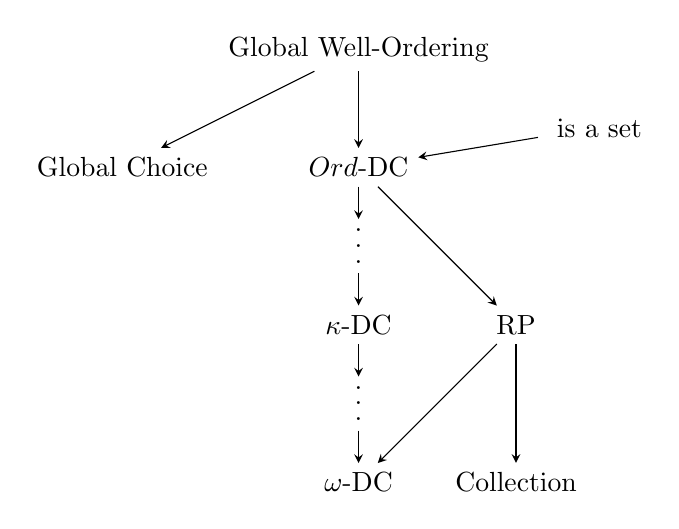
\begin{tikzpicture}
\begin{scope}[every node/.style={}]
    \node (A) at (8, -2.5) {Collection};
    \node (B) at (9, 2){$\A$ is a set};
    \node (C) at (3, 1.5){Global Choice};
    \node (D) at (6,1.5) {$Ord$-DC };
    \node (E) at (6, -0.5) {$\kappa$-DC};
    \node (I) at (8, -0.5) {RP};


    \node (L) at (6, 0.7) {.};
    \node (M) at (6, 0.5) {.};
    \node (N) at (6, 0.3) {.};
    \node (P) at (6, -1.7) {.};
    \node (Q) at (6, -1.5) {.};
    \node (R) at (6, -1.3) {.};
    \node (S) at (6, -2.5) {$\omega$-DC};
    \node (T) at (6, 3) {Global Well-Ordering};
    
\end{scope}

\begin{scope}[>={stealth},
              every node/.style={fill=white,circle},
              every edge/.style={draw=black}]

    \path [->] (T) edge (D);
\path [->] (T) edge (C);
     \path [->] (B) edge (D);
     


    \path [->] (I) edge (A);
      \path [->] (I) edge (S);
    \path [->] (D) edge (I);
    \path [->] (D) edge (L);
    \path [->] (N) edge (E);
    \path [->] (E) edge (R);
     \path [->] (P) edge (S);
       
\end{scope}
\end{tikzpicture}
 \caption{Implication diagram in $\GBUR$}
 \label{GBUdiagram}
\end{center}
\end{figure}
\FloatBarrier
\subsection{Interpreting $\mathcal{U}$ in $\mathcal{V}$}\label{section:interpretingUrelementsinClassTheory}
The construction of $V\llbracket X \rrbracket$ introduced in Section \ref{section:interpretingUinV} can be easily generalized to interpreting urelement class theory in pure class theory.
\begin{definition}\label{barwiseinterpretation2}
Let $\<V, \in , \mathscr{V}>$ be a model of GBc and $X \in \mathscr{V}$. $\<V \llbracket X \rrbracket, \bar{A}, \bar{\in}>$ is then defined as in Definition \ref{barwiseinterpretation1}. Let $\mathscr{V}\llbracket X \rrbracket = \{Y \in \mathscr{V} : Y \subseteq  V \llbracket X \rrbracket\}$. $\mathscr{V}\llbracket X \rrbracket$ denotes the model $\< V \llbracket X \rrbracket, \bar{A}, \bar{\in}, \mathscr{V}\llbracket X \rrbracket>$.\footnote{Note that when $Y \in \mathscr{V}\llbracket X \rrbracket$, $\mathscr{V}\llbracket X \rrbracket \models x \in Y$ if and only if $\mathscr{V} \models x \in Y$.}
\end{definition}

\begin{theorem}\label{Con(KM)->Con(KMU)}
Suppose $\mathscr{V} \models $ GBc and $X$ is a class in $\mathscr{V}$. Then
\begin{enumerate}
    \item $\mathscr{V}\llbracket X \rrbracket \models $ $\GBUR$ + Collection;
    \item $\mathscr{V}\llbracket X \rrbracket \models $ $\KMUR$ + Collection if $\mathcal{V} \models$ KMc;
    \item $\mathscr{V}\llbracket X \rrbracket \models $ CC if $\mathscr{V} \models$ CC;
    \item $\mathscr{V}\llbracket X \rrbracket \models $ Limitation of Size (and hence GBCU) if $\mathcal{V} \models$ GBC.
\end{enumerate}
\end{theorem}

\begin{proof}


For (1) and (2), $\mathscr{V}\llbracket X \rrbracket \models$ ZU by Theorem \ref{thm:V[X]modelsZFU}, so it remains to show that $\mathscr{V}\llbracket X \rrbracket$ satisfies Collection, Class Extensionality, and First-Order Comprehension (or Full Comprehension), all of which follow easily from the fact that $\mathscr{V} \models$ GBc (or KMc). For example, to show $\mathscr{V}\llbracket X \rrbracket \models$ Collection, suppose that in $\mathscr{V}\llbracket X \rrbracket$ for every $x \in \barw$ there is some $y$ such that $x \bar{R} y$ for some $\barw, \bar{R} \in \mathscr{V}\llbracket X \rrbracket$, where $\barw = \<1, w>$. Then in $V$ there is some $v \subseteq V \llbracket X \rrbracket$ such that for every $\barx \in w$, there is some $\bary \in v$ such that $\mathscr{V}\llbracket X \rrbracket \models \<\barx, \bary> \in \bar{R}$. Then $\bar{v} = \<1, v>$ is a desired collection set in $\mathscr{V}\llbracket X \rrbracket$.

(3) Suppose that $\mathscr{V} \models$ CC AND for every $\barx \in V\llbracket X \rrbracket$, there is some class $\bar{X} \in \mathscr{V}\llbracket X \rrbracket$ with $\varphi(\barx, \bar{X}, \bar{Z})^{ \mathscr{V}\llbracket X \rrbracket}$. By CC in $\mathscr{V}$, there is a class $Y \subseteq V\llbracket X \rrbracket \times U$ such that for every $\barx \in V\llbracket X \rrbracket$, $\varphi(\barx, Y_{\barx}, \bar{Z})^{ \mathscr{V}\llbracket X \rrbracket}$ and $Y_{\barx} $ is a class of $\mathscr{V}\llbracket X \rrbracket$. Define $\overline{Y} = \{\overline{\<\barx, \bary>} : \bary \in Y_{\barx} \land \barx \in \mathscr{V}\llbracket X \rrbracket \}$ (where $\overline{\<\barx, \bary>}$ codes the ordered-pair as in Theorem \ref{thm:ACholdsViffACholdsinV[X]}), which is a class of $\mathscr{V}\llbracket X \rrbracket$. Since for every $\barx \in \mathscr{V}\llbracket X \rrbracket$, $\mathscr{V}\llbracket X \rrbracket \models Y_{\barx} = \overline{Y}_{\barx}$, it follows that CC holds in $\mathscr{V}\llbracket X \rrbracket$.

(4) Suppose that $\mathscr{V}$ Global Well-Ordering. Note that if $\bar{Y}$ and $\bar{Z}$ are two proper classes in $\mathscr{V}\llbracket X \rrbracket$ , they must be equinumerous proper classes in $\mathscr{V}$ by Propostion \ref{prop:GC<->GWO<->LS}. So in $\mathscr{V}$ there must be a bijection $F$ between $\bar{Y}$ and $\bar{Z}$. Then $\bar{F} = \{ \overline{\<\bary, \barz>} : F(\bary) = \barz \}$ will be a bijection between $\bar{Y}$ and $\bar{Z}$ in $\mathscr{V}\llbracket X \rrbracket$.\end{proof}


\begin{theorem}\label{KMU+LSbiintepsKM+LS}
The following pairs of theories are bi-interpretable with parameters.
\begin{enumerate}
    \item GBC and GBCU + $\A \sim \omega$;
    \item KMC and KMCU + $\A \sim \omega$;
    \item GBC and GBCU + Limitation of Size;
    \item KMC and KMCU + Limitation of Size;
    \item GBC and GBCU + Limitation of Size + Plenitude;
    \item KMC and KMCU + Limitation of Size + Plenitude.
\end{enumerate}
\end{theorem}
\begin{proof}
Working in GBC (KMC), we can form either $\mathscr{V}\llbracket \omega \rrbracket$ (or $V\llbracket Ord\rrbracket$), and the map $y \mapsto \hat{y}$ and $Y \mapsto \hat{Y} = \{\hat{y} : y \in Y\}$ will be a definable isomorphism between $\mathcal{V}$ and $V^{\mathcal{V}\llbracket \omega \rrbracket}$ (or $V^{\mathcal{V}\llbracket Ord \rrbracket}$). In KMCU + Limitation of Size, there will be an injective map $F$ from $\A$ to $V$. For every urelement $a$, let $\tilde{a} = \<0, F(a)>$; and for every set $x$, we let $\tilde{x} = \<1, \{\tilde{y} : y \in x\}>$. It follows by an easy induction that the map $x \mapsto \tilde{x}$ and $X \mapsto \tilde{X} = \{\tilde{x} : x \in X\}$ is an isomorphism between $U$ and $V\llbracket F[\A] \rrbracket$.
\end{proof}

\begin{corollary}\label{corollary:LS<->AlessthanV}
Over KMCU, the following are equivalent.
\begin{enumerate}
    \item Limitation of Size.
    \item There is an injective map from $\A$ to $V$.
\end{enumerate}
\end{corollary}
\begin{proof}
(1) $\rightarrow$ (2) is clear. For (2) $\rightarrow$ (1), first observe that over KMCU, Limitation of Size holds for the pure classes $\mathcal{V}$. For, given a global choice function, its restriction to $V$ is a pure class so $\mathcal{V} \models $ Global Choice, which means $\mathcal{V} \models $ Limitation of Size by Proposition \ref{prop:GC<->GWO<->LS}. Now suppose that $F$ is an injective map from $\A$ to $V$. Since $U$ and $V\llbracket F[\A] \rrbracket$ are equinumerous, every proper class is equinumerous with a pure proper class. Therefore, all proper classes are equinumerous.
\end{proof}

\subsection{Independence results}\label{section:independenceinClassTheory}
In this subsection, I discuss several independence results concerning the completeness of Diagram \ref{GBUdiagram} over $\KMUR$. To begin with, arguments in \ref{subsection:implicationdiagram} which appeal to homogeneity can no longer go through in the context of class theory. For example, one might attempt to show that $\KMUR$ + Plenitude implies $\omega$-DC by the same argument as in Theorem \ref{Plenitude->DCS}. But the problem is that the ``kernel'' of a class relation $R$ might be a proper class, in which case we cannot find some a set of urelements that is big enough to ``fix'' $R$. In fact, we will see that over $\KMUR$,
\begin{enumerate}
    \item $\kappa$-DC $\nrightarrow$ Collection;
    \item Global Choice  $\nrightarrow$ ($\omega$-DC $\lor$ Collection);
    \item Collection $\nrightarrow$ $\omega$-DC;
    \item RP $\nrightarrow$ $\omega_1$-DC.
\end{enumerate}
Since it is well-known that KMc cannot prove Global Well-Ordering, it follows that Diagram \ref{GBUdiagram} is indeed complete over $\KMUR$.

Let me first discuss a general method of constructing \textit{class permutation models} of $\KMUR$ used in \cite{felgner1976choice}. Given a model $\<U, \A, \in, \U>$ of KMCU, we might fix an $\A$-ideal $\I$ as in Definition \ref{normalideal} and consider $U^\I$, the class of all first-order objects whose kernel is small in the sense of $\I$. This will give us a model of $\ZFCUR$ as before. To have a model of $\KMUR$, however, we cannot take all subclasses of $U^I$ as the second-order part of $U^\I$. To see this, suppose that $\A$ is an infinite set and $\I$ is its ideal of finite subsets; then an injection $F$ from $\omega$ to $\A$ will be a subclass of $U^\I$, which means having $F$ as a class of the model we intend to build would violate Replacement. In other words, we need to throw out some subclasses of $U^\I$. This is done by finding some suitable group $\G$ of permutations on $\A$ and only keep those subclasses of $U^\I$ that are \textit{symmetric} with respect to $\I$ and $\G$.

\begin{definition}[KMCU]
Let $\G$ be a group of permutations of $\A$.\footnote{It is understood that every $\pi \in \G$ is a permutation of a \textit{set} of urelements. Whenever $\pi, \sigma \in \G$, $\pi \circ \sigma$ is taken as the composition of their canonical extensions, which point-wise fix the urelements not in their original domains.} For any $x \in U$, $sym(x)$ and $fix(x)$ are defined as in Definition \ref{permutationmodeldef}. Let $\I\in \U$ be an $\A$-ideal as in Definition \ref{normalideal}. $\I$ is said to be $\G$-\textit{flexible} if 
\begin{enumerate}
    \item for every $\pi \in \G$ and $A \in \I$, $\pi A \in \I$;
    \item $\I$ has a \textit{basis} such that for every $B$ in the basis and $ A \in \I$ disjoint from $B$, there is some $\pi \in fix(B)$ such that $\pi A \neq A$.
\end{enumerate}
A class $X$ is \textit{symmetric} (w.r.t. $\G$ and $\I$) if there is some $A \in \I$, called a \textit{support} of $X$, such that $fix(A) \subseteq sym(X)$, where $sym(X) = \{\pi \in \G : \pi X = X\}$.  $U^\I =\{ x\in U : ker(x) \in \I\}$. $\W = \{ X \subseteq U^\I : X \text{ is symmetric}\}$. The model $\<U^\I, \in, \A, \W>$ is also denoted by $\W$.
\end{definition}
\noindent As we shall see later, $\G$-flexibility ensures that enough classes are thrown out so that Replacement can hold in $\W$. It is easy to check that every $\pi \in \G$ is an automorphism of $\W$ because $\I$ is $\G$-flexible.

\begin{theorem}[KMCU]\label{classpermutationmodel}
Let $\G$ be a group of permutations on $\A$ and $\I$ be an $\A$-ideal that is $\G$-flexible. Then $\W \models \KMUR$. 
\end{theorem}
\begin{proof}
$\W$ is a transitive class containing all the urelements and pure sets. And by the same argument as in Theorem \ref{smallkernelmodel}, it follows that $\W \models $ ZU + AC + Separation + Class Extensionality.  


To show $\W \models$ Replacement, suppose that $x \in \W$ be a set and $F \in \W$ be a class function on $x$ with a support $A \in \I$. Let $\mathcal{J}$ be a basis of $\I$ which witnesses its flexibility and $B$ be a set of urelements in $\J$ with $ker(x) \cup A \subseteq B$. It suffices to show that $ker(F[x]) \subseteq B$. If not, then there is some $y \in F[x]$ such that $ker(y) \setminus B$ is not empty. Since $ker(y) \setminus B \in \I$, it follows that there is some $\pi \in fix(B)$ such that $\pi (ker(y) \setminus B) \neq ker(y) \setminus B$, and as a result, $\pi y \neq y$. But $F(z) = y$ for some $z \in x$ so $F(z) = \pi y$, which is a contradiction.


To show that Full Comprehension holds in $\W$, fix a formula $\varphi$ in the language of urelement class theory and classes $X_0, .., X_n \in \W$, in $\U$ let $X = \{ x \in  \W: \W \models \varphi (x, X_0, ... ,X_n \}$. It suffices to show that $sym(X_0) \cap ... \cap sym(X_n) \subseteq Sym(X)$. Fix a $\pi \in sym(X_0) \cap ... \cap sym(X_n)$. For every $x \in X$, since $\pi$ is an automorphism of $\W$, it follows that $\W \models \varphi (\pi x, X_0, ..., X_n)$ and hence $\pi x \in X$. Therefore, $\pi X = X$.
\end{proof}
\begin{theorem}\label{thm:KMUR+kDCvdashCollection}
Assume the consistency of KM. Let $\kappa$ be any infinite cardinal. There is a model of $\KMUR$ in which
\begin{enumerate}
    \item $\kappa$-DC holds;
    \item Collection fails.
\end{enumerate}
\end{theorem}
\begin{proof}
Let $\U$ be a model of KMCU + $\A \sim \aleph_{\kappa^+}$. Let $\I$ be the ideal of all sets of urelements of size less than $\aleph_{\kappa^+}$ and $\G$ be the group of all permutations of $\A$. It is clear that $\I$ is $\G$-flexible, so the resultant model $\W$ satisfies $\KMUR$. Collection fails in $\W$ because every cardinal below $\aleph_{\kappa^+}$ is realized while $\aleph_{\kappa^+}$ is not. To show $\kappa$-DC holds in $\W$, suppose that $R$ is a class relation in $\W$ without terminal nodes. Since the first-order domain of $\W$, $U^\I$, is closed under $\kappa$-sequences, $\U$ thinks that $\forall s \in (U^\I)^{<\kappa} \exists y \in U^\I R(x, y)$; by $Ord$-DC in $\U$, it follows that there is an $f \in (U^\I)^{\kappa}$ such that $R(f\restriction \alpha, f(\alpha))$ for every $\alpha < \kappa$. $f$ lives in $U^\I$, so $\kappa$-DC holds in $\W$.
\end{proof}


\begin{theorem}[Felgner \cite{felgner1976choice}]\label{thm:KMURnvdashCollection}
Assume the consistency of KM. There is a model of $\KMUR$ in which
\begin{enumerate}
    \item Global Choice holds;
    \item $\omega$-DC fails;
    \item Collection fails.
\end{enumerate}
\end{theorem}
\begin{proof}
Let $\U$ be a model of KMCU + $\A \sim \omega$, in which we identify $\A$ with the rationals $\<\Q, <_\Q>$. Let $\G$ be the group of permutations of $\A$ that preserves $<_\Q$ and $\I$ be the ideal of finite subsets of $\A$. $\I$ is $\G$-flexible: if $A, B \in \I$ are disjoint, for any $b \in B \setminus A$, there is an open interval containing $b$ that is disjoint from $A \cup B \setminus \{b\}$; so we can permute this interval in an order-preserving way and leave $A$ point-wise fixed. By Theorem \ref{classpermutationmodel}, it follows that the resultant class permutation model $\W$ satisfies $\KMUR$. Moreover, both Collection and $\omega$-DC fail in $\W$ since there is a proper class of urelements but every set of them is only finite. For a proof of $\W \models$ Global Choice, see \cite[pp. 249-250]{felgner1976choice} or \cite[Lemma 2.3]{yao2022reflection}. \end{proof}

\begin{theorem}\label{kmudoesnotproveDC}
Assume the consistency of KM. There is a model of $\KMUR$ in which 
\begin{enumerate}
    \item Collection holds;
    \item Plenitude holds;
    \item $\omega$-DC fails.
\end{enumerate}
\end{theorem}

\begin{proof}
The model used here is also due to Felgner\cite{felgner1976choice}. The point here is that the model also satisfies Collection, which is not discussed in Felgner's paper. Let $\U$ be a model of KMCU with an enumeration of $\A$ with the tree $Ord^{<\omega}\setminus \{\emptyset\}$ consisting of all non-empty finite sequences of ordinals. Each urelement is identified with a node on the tree and define $a \lhd b$ as $a \subsetneq b$. $b$ is said to be an \textit{immediate descendant} of $a$ if $b$ extends $a$ by one digit. $b$ and $b'$ are \textit{siblings} if either they are both top nodes, or they are an immediate descendant of the same node. A set $t \subseteq \A$ is a \textit{tree} if it is closed under initial segment (i.e, if $b \in t$ and $a \lhd b$, then $a \in t$). A \textit{path} of a tree $t$ with length $\alpha$ is a function $f: \alpha \rightarrow Ord$ such that $f\restriction \beta \in t$ for all $\beta < \alpha$. A \textit{branch} is a maximal path, i.e., it is not properly extended by any path of the tree. A tree $t$ is \textit{small} if it has no infinite branch. Let $\T$ be the class of all small trees, which forms a basis for an ideal $\I$. Let $\G$ be the group of  permutations of $\A$ that preserves $\lhd$.
\begin{lemma}\label{treeflexible}
$\I$ is $\G$-flexible with respect to the basis $\T$.
\end{lemma}
\begin{proof}
If $a$ and $b$ are siblings with domain $n + 1$, then there is a natural permutation $\pi^a_b \in \G$ such that for every node $c$ with $dom(c) = j +1$ and $i < j+1$,
\begin{equation*}
   \pi^a_b c (i)  =
    \begin{cases*}
      b(n) & if $i = n$, $c(n) = a(n)$ and $c \restriction n = a \restriction n$  \\
      a(n) & if $i = n$, $c(n) = b(n)$ and $c \restriction n = a \restriction n$  \\
      c(i) & otherwise
    \end{cases*}
 \end{equation*}
 $\pi^a_b$ thus swaps only $a$ and $b$ and their descendants. Given a small tree $t$ and some $A \in \I$ disjoint from $t$, since every node has  $Ord$-many siblings we can find a node $a$ in $A$ and a sibling $b$ of $a$ such that $b \notin t \cup A$. $\pi^a_b$ will then leave $t$ point-wise fixed because $t$ is a tree.
\end{proof}
\noindent Therefore, the class permutation model $\W$ given by $\G$ and $\I$ satisfies $\KMUR$. $\W$ clearly satisfies Plenitude because for every $\kappa$, there are $\kappa$-many top nodes on the tree $Ord^{<\omega}\setminus \{\emptyset\}$. Suppose \textit{for reductio} that $\omega$-DC holds in $\W$. Since in $\W$ every $a \in \A $ has some $b \in A$ such that $a \lhd b$, then in $\W$ there is an infinite branch $s = \<a_n : n < \omega>$ such that $a_n \lhd a_{n+1}$ for every $n$. Let $t$ be a small tree such that $fix(t) \subseteq sym(s)$. Fix some $a_n$ not in $t$ and some sibling $b$ of $a_n$ such that $b \notin t$. Then $\pi_{a_n, b} \in fix(t)$ but $\pi_{a_n, b} (s) \neq s$, which is a contradiction.

It remains to show that $\W \models$ Collection. For any two small tress $t$ and $t'$, we say that $t$ \textit{mildly extend} $t'$ if $t' \subseteq t$ and no branch of $t$ properly extends a branch of $t'$.


\begin{lemma}\label{treelemma}
Let $t_0, t_1 \in \T$ be such that $t_0 \subseteq t_1$ and every terminal node in $t_0$ has a descendent in $t_1$. Then for every $t \in \T$, there is a $\pi \in fix(t_0)$ such that $ t_1 \cup \pi t $ mildly extends $t_1$.  
\end{lemma}
\begin{proof}
Define $M = \{ a \in t_1 \setminus t_0 : a \text{ is an initial node in } t_1 \setminus t_0 \text{ and } a \text{ has a descendant in } t\}$, where ``$a$ initial in $t_1 \setminus t_0$'' means there is no node $b \in t_1 \setminus t_0$ such that $b \lhd a$. Since every node has $Ord$-many siblings and Global Well-Ordering holds in $\U$, for every $a \in M$ we can pick a sibling $a'$ of $a$ such that $a' \notin t_1 \cup t$, and we can ensure that $a_1' \neq a_2'$ for any distinct  $a_1, a_2 \in M$. Let $\pi = \bigcup_{a \in M}\pi^a_{a'}$, which is in $\G$. $\pi \in fix(t_0)$, because no node in $t_0$ is a descendant of any node in $M$ and $\pi$ only moves nodes in $M$ and their descendants.

To show that $t_1 \cup \pi t $ mildly extends $t_1$, consider any branch $f$ of $t_1$. Suppose \textit{for reductio} that $f$ is properly extended by a branch $g$ of $\pi t$. Note that $f$ must contain a node not in $t_0$ since otherwise $f$ would be a branch of $t_0$, which is impossible because every branch of $t_0$ is properly extended by a branch of $t_1$. So let $a$ be the least such node. There is a node $b$ on $g$ such that $a \lhd b$, where $b =\pi c$ for some $c \in t$. It follows that $a$ must be in $M$. If not, then $\pi a = a$ so $a \lhd c$ and hence $a$ is in $M$ after all. Thus, $\pi a = a'$ for some $a' \notin t$, but then $a' \lhd c$ so $a' \in t$---contradiction.
\end{proof}

\begin{lemma}
For any infinite cardinal $\kappa$, if $\<t_\alpha : \alpha < \kappa>$ is a sequence of small trees such that $t_\alpha$ mildly extends $\bigcup_{\beta < \alpha} t_\beta$ for every $\alpha < \kappa$, then $\bigcup_{\alpha < \kappa} t_\alpha$ is a small tree.
\end{lemma}
\begin{proof}
Let $t= \bigcup_{\alpha < \kappa} t_\alpha$. Suppose \textit{for reductio} that $f$ is an infinite branch of $t$. There will be some $t_\alpha$ with some $0 < m < \omega$ such that $f\restriction m$ is a branch of $t_\alpha$. Then for some $\beta > \alpha$, $t_\beta$ contains a branch that extends $f \restriction m$, which contradicts the assumption.
\end{proof}

Now suppose that $\W \models \forall x \in w \exists y \<x, y> \in R$ for some $w, R \in \W$. Let $t_0$ be a small tree that includes $ker(w)$ and some support of $R$, and enumerate $w$ by $\{x_\alpha : \alpha <\kappa\}$ for some $\kappa$. In $U$, we define a $\kappa$-sequence of small tress $\<t_\alpha : \alpha < \kappa>$ such that 
\begin{itemize}
    \item [] (i) $t_\alpha$ mildly extends $\bigcup_{\beta < \alpha} t_\beta$ for every $\alpha < \kappa$;
    \item [] (ii) for each $x_\alpha$, there is some $y \in \W$ such that $\<x_\alpha, y> \in R$ and $ker(y) \subseteq  t_\alpha$.
\end{itemize}
This is possible, because for every $x_\alpha$, fix some $y'$ with $\<x, y'> \in R$. Since $ker(y')$ is a subset of some small tree $t$, by Lemma \ref{treelemma}, there is a $\pi \in fix (t_0)$ such that $\bigcup_{\beta < \alpha} t_\beta \cup \pi t$ mildly extends $\bigcup_{\beta < \alpha} t_\beta$. Thus $\<x_\alpha, \pi y'> \in R$ and $ker(\pi y') \subseteq \pi t$. Let $t_\kappa = \bigcup_{\alpha < \kappa} t_\alpha$, which is a small tree. It follows that $\forall x \in w \exists y \in V(t_\kappa) \ (\<x, y> \in R)$, which suffices for Collection in $\W$.
\end{proof}
\noindent By using the same argument at the previous theorem, it is not hard to show that $\W \models \kappa$-CC for every infinite cardinal $\kappa$. However, it is unclear if the model $\W$ in Theorem \ref{kmudoesnotproveDC} satisfies CC if we assume $\U \models$ CC. 


\begin{theorem}\label{thm:RPnvdashOmega1Dc}
Assume the consistency of KM. There is a model of $\KMUR$ in which 
\begin{enumerate}
    \item RP holds;
    \item Plenitude holds;
    \item $\omega_1$-DC fails.
\end{enumerate}
\end{theorem}
\begin{proof}
Let $\U$ be a model of KMCU with an enumeration of $\A$ with the tree $Ord^{<{\omega_1}}\setminus \{\emptyset\}$ consisting of all non-empty \textit{countable} sequences of ordinals. A set $t$ of urelements is an $\omega_1$-small tree if it is a tree without any $\omega_1$-branch. Let $\I$ be the ideal generated by all the $\omega_1$-small trees and $\G$ be the group of permutations of $\A$ that preserve the tree structure as in the proof of Theorem \ref{kmudoesnotproveDC}. Since the same arguments in Lemma \ref{treeflexible} and \ref{treelemma} still go through, it follows that $\I$ is $\G$-flexible and that Collection holds in the resultant model $\W$.
\begin{claim}
$\W \models $ RP. 
\end{claim}
\begin{claimproof}
By Proposition \ref{prop:rp+gbur<->collection+dcs}, it is enough to show that $\omega$-DC holds in $\W$. So it suffices to show that the ideal $\I$ is countably closed. This is simply because the union countably many $\omega_1$-small trees, $\{t_n : n< \omega \}$, is an $\omega_1$-small tree. 
\end{claimproof}
\begin{claim}
$\W \models $ $\neg$($\omega_1$-DC).
\end{claim}
\begin{claimproof}
Suppose \textit{for reductio} that $\omega_1$-DC holds in $\W$. Say that a sequence $s \in \A^\alpha$ is a \textit{chain} if $s(\beta) \lhd s(\beta')$ for every $\beta < \beta' < \alpha$; and $s$ is said to be \textit{bound} by $a$ if $s(\beta) \lhd a$ for every $\beta < a$. In $\W$, every chain $s\in \A^{<\omega_1}$ has a bound $a \in \A$. By  $\omega_1$-DC, in $\W$ there is an $f \in \A^{\omega_1}$ that is a chain of length $\omega_1$. Then $ker(f)$ must be contained in some $\omega_1$-small tree, which is impossible.
\end{claimproof}

\end{proof}

\subsection{Open questions}
It is a classic result that GBC is a conservative extension of ZFC (e.g., see \cite{felgner1976choice}). But we know that GBCU is \textit{not} a conservative extension of ZFCU: GBCU proves that either $\A$ is a set, or Plenititude holds, which is not provable in ZFCU.
\begin{question}
\
\begin{enumerate}
    \item Is $\GBUR$ + Global Choice conservative over $\ZFCUR$?
    \item Is $\GBUR$ + Collection + Global Choice conservative over ZFCU?
\end{enumerate}
\end{question} 
\noindent Given Theorem \ref{kmudoesnotproveDC} and the fact that CC is a stronger version of Collection, it is natural to ask the following.
\begin{question}
Does $\KMUR$ prove any of the following?
\begin{enumerate}
    \item Collection $\land$ Global Choice $\rightarrow$ $\omega$-DC.
    \item CC $\rightarrow$ $\omega$-DC.
    \item CC $\land$ Global Choice $\rightarrow$ $\omega$-DC.
\end{enumerate}
\end{question}
A natural question arises at this point as in Section \ref{section:WhatisZFCU}: what is KMc (or, GBc) class theory with urelements if we only wish to have AC for sets? Notably, in both class and set theory with urelements, Collection tends to lose its strength without enough choice. As previously conjectured, $\ZFUR$ + Collection does not prove RP, and in fact, $\ZFUR$ + DC should not be able to prove the DC$_\omega$-scheme. Theorem \ref{kmudoesnotproveDC} confirms that this is indeed the case in urelement class theory. Thus, although Collection is still strictly stronger than Replacement in class theory with urelements, adding it into $\KMUR$ cannot produce a theory with sufficient strength. So perhaps a robust version of KMc with urelements \textit{should} include RP as an axiom since it implies $\omega$-DC (Proposition \ref{prop:rp+gbur<->collection+dcs}). However, RP cannot exclude \textit{all} pathological models: in the proof of Theorem \ref{thm:RPnvdashOmega1Dc}, the model satisfies RP but contains a $Ord$-splitting tree without any $\omega_1$-branch. That said, it seems that bringing urelements back to the picture inevitably invites \textit{axiomatic freedom}.





\section{Second-order reflection with urelements}\label{section:RP2withurelements}

\subsection{Bi-interpretabtion with few urelements}
The second-order reflection principle (first introduced by Bernays \cite{bernays1976problem}) is the  scheme

\begin{itemize}
    \item [] (RP$_2$) $\forall X [\varphi(X) \rightarrow \exists t( t \text{ is transitive} \land \varphi^t(X \cap t))]$,
\end{itemize}
where $\varphi$ can be any formula in the language of class theory, and $\varphi^t$ is the result of restricting all the first-order quantifiers to the members of $t$ and all the second-order quantifiers to the subsets of $t$. Thus, $\varphi^t(X \cap t)$ is simply the assertion $\<t, \in, P(t)> \models \varphi(X \cap t)$. As observed in \cite{bernays1976problem} and \cite{tait2005constructing}, RP$_2$ is able to ``bootstrap''. For example, with the Axiom of Separation, Foundation and Extensionality, RP$_2$ can recover the remaining axioms of KMC.

\begin{prop}
RP$_2$ + Separation + Extensionality + AC + Foundation $\vdash$ KMCU + CC. 
\end{prop}
\begin{proof}
Note that RP alone implies that every $x_1, ..., x_n$ will be contained in some transitive set since we can reflect the formula $\exists y (x_1 = y) \land ... \land \exists y (x_n =y)$. This implies Pairing and Union given Separation. Then we can reflect the assertion ''for every $x$,  $x \cup \{x\}$ exists" down to a transitive set to get Infinity. Collection (and hence Replacement) follows by Proposition \ref{prop:rp+gbur<->collection+dcs}. To get Powerset, note that for every set $u$, by Separation we have ``for every class $X$ that is a subclass of $u$, there is a set $x$ that is co-extensional with $X$''. So by RP$_2$ we can reflect this assertion down to some transitive set $t$ containing $u$. Accordingly, $t$ contains every subset of $u$ as a member, which suffices for Powerset given Separation.

For Class Choice, suppose \textit{for reductio} that $\forall x \exists X \varphi(x, X, Z)$ for some class $Z$ but there is no $Y \subseteq U \times U$ such that $\varphi(x, Y_x, Z)$. By RP$_2$, there is some transitive set $t$ such that $\forall x \in t \exists X \subseteq t \varphi^t(x, X, Z \cap t)$ and there is no $Y \subseteq t\times t$ such that $\forall x \in t \varphi^t (x, Y_x, Z \cap t)$. Since there is a well-ordering of $P(t)$, for every $x \in t$ we can choose a $y_x \in P(t)$ such that $\varphi^t(x, y_x, Z\cap t)$. Let $Y = \bigcup_{x \in t}\{\<x, z> : z \in y_x\}$. It follows that $\forall x \in t \varphi^t (x, Y_x, Z \cap t)$, which is a contradiction.

Similarly, to show that there is a global well-ordering, we suppose \textit{for reductio} that there is no global well-ordering and reflect this statement to some transitive set $t$ that is closed under pairs. Since there is a well-ordering of $t$, the reflected statement will yield a contradiction.

Finally, we also get Full Comprehension. This is because if there is a failure of Full Comprehension of the form $\neg \exists X \forall z (z \in X \leftrightarrow \varphi(x, P))$, then we can reflect it down to some transitive $t$ to get $\neg \exists x \subseteq t \forall z (z \in x \leftrightarrow \varphi^t(x, P \cap t))$, which will then contradict Separation.\footnote{As a consequence, note that RP$_2$ is equivalent to the following scheme, which asserts that every statement, possibly with class parameters, is absolute to some transitive set.
\begin{itemize}
    \item [] (RP$_2^+$) $\forall X \exists \text{ transitive } t (\varphi(X) \leftrightarrow \varphi^t(X \cap t))$.
\end{itemize}
This is because given $\varphi$ and some class $X$, by Full Comprehension we can form the class $Y$ such that $\forall y (y \in Y \leftrightarrow \varphi(X))$; then by RP$_2$, there will be a non-empty transitive set $t$ such that $\forall y \in t (y\in Y\cap t \leftrightarrow \varphi^t(X \cap t))$. It follows that $\varphi(X) \leftrightarrow \varphi^t (X \cap t)$.}\end{proof}

In pure class theory, the bootstrapping of RP$_2$ goes beyond KMC as it yields large cardinals. In particular, RP$_2$ implies the exsitence of a proper class of inaccessible cardinals, Mahlo cardinals and weakly compact cardinals (see \cite{tait2005constructing} for more on this). However, the consistency strength of RP$_2$ is bounded by ZFC + an $\omega$-Erd{\"o}s cardinal (see \cite[Exercise 9.18]{kanamori2008higher}), which is consistent with $V = L$. Some natural question arise in the context of urelements: What is the consistency strength of RP$_2$ in urelement class theory? Could it be somehow affected by urelements? 

The next lemma shows that the $\mathcal{V} \llbracket X \rrbracket$ construction introduced in Definition \ref{barwiseinterpretation2} preserves second-order reflection.
\begin{lemma}\label{lemma:KM+RP2interpretsKMU+RP2}
Let $\mathcal{V} \models$ KM + RP$_2$ and $W \in \mathcal{V}$ be a class. Then $\mathcal{V} \llbracket W \rrbracket \models $ KMU + RP$_2$ + Limitation of Size.
\end{lemma}
\begin{proof}
Since RP$_2$ + KM proves that there is a global well-ordering, which implies Limitation of Size over KM, by Theorem \ref{Con(KM)->Con(KMU)} it follows that $\mathcal{V} \llbracket W \rrbracket \models $ KMU + Limitation of Size. So it remains to show that every instance of RP$_2$ holds in $\mathcal{V} \llbracket W \rrbracket$. For every transitive set $t \in V$, let $t\llbracket W \rrbracket = \<1, V\llbracket W \rrbracket \cap t>$, which is a transitive set in $V\llbracket W \rrbracket$.

\begin{claim}\label{permu}
Let $t$ be a transitive set in $\mathcal{V}$. Then for any $x_1, ... x_n \in t\llbracket W \rrbracket$ and $X_1, ... ,X_m \in \mathcal{V} \llbracket W \rrbracket$, $ \mathcal{V} \models (\varphi^{\mathcal{V} \llbracket W \rrbracket})^t \leftrightarrow (\varphi^{t\llbracket W \rrbracket})^{\mathcal{V} \llbracket W \rrbracket}$ for any suitable formula $\varphi$ in the language of urelement class theory.
\end{claim}
\begin{claimproof}
If $\varphi$ is an atomic formula, then the claim holds because the definition of $\bar{\in}$ and $\bar{\A}$ (see Definition \ref{barwiseinterpretation1}) is absolute for transitive sets. Boolean cases commute. And if $\varphi$ is $\exists x \psi$, we have
\begin{align*}
    (\varphi^{\mathcal{V} \llbracket W \rrbracket})^t  &= (\exists x \in \mathcal{V} \llbracket W \rrbracket  \psi^{\mathcal{V} \llbracket W \rrbracket})^t \\
                &\Leftrightarrow \exists x \bar{\in} t\llbracket W \rrbracket (\psi^{\mathcal{V} \llbracket W \rrbracket})^t \\
                & \Leftrightarrow \exists x \bar{\in} t\llbracket W \rrbracket (\psi^{t\llbracket W \rrbracket})^{\mathcal{V} \llbracket W \rrbracket} \tag*{(by induction hypothesis)} \\
                & = (\varphi^{t\llbracket W \rrbracket})^{\mathcal{V} \llbracket W \rrbracket}.
\end{align*}
Similarly, if $\varphi$ is $\exists X \psi$, then we have
\begin{align*}
    (\varphi^{\mathcal{V} \llbracket W \rrbracket})^t  &= (\exists X \subseteq V \llbracket W \rrbracket  \psi^{\mathcal{V} \llbracket W \rrbracket})^t \\
                &\Leftrightarrow \exists X \subseteq t\llbracket W \rrbracket (\psi^{\mathcal{V} \llbracket W \rrbracket})^t \\
                & \Leftrightarrow \exists  X \subseteq t\llbracket W \rrbracket (\psi^{t\llbracket W \rrbracket})^{\mathcal{V} \llbracket W \rrbracket} \tag*{(by induction hypothesis)}\\
                & = (\varphi^{t\llbracket W \rrbracket})^{\mathcal{V} \llbracket W \rrbracket}.
\end{align*}
This proves the claim.                                                  \end{claimproof}

Now if $\mathcal{V} \llbracket W \rrbracket \models \varphi$, then we can reflect $\varphi^{\mathcal{V} \llbracket W \rrbracket}$ in $\mathcal{V}$ down to some transitive set $t$. By the claim, it follows that $\mathcal{V} \llbracket W \rrbracket \models \varphi ^{t\llbracket W \rrbracket}$. Hence, $\mathcal{V} \llbracket W \rrbracket \models$ RP$_2$. \end{proof}
\begin{theorem}\label{KM + RP <-> KMU + RP + LS}
KM + RP$_2$ and KMU + RP$_2$ + Limitation of Size are bi-interpretable with parameters. \qed
\end{theorem}
\begin{proof}
First note that KMU + RP$_2$ also interprets KM + RP$_2$, because if $\mathcal{U} \models$ KMU + RP$_2$, then its pure part $\mathcal{V} \models$ KM + RP$_2$. For, as in Lemma \ref{lemma:KM+RP2interpretsKMU+RP2}, given a transitive $t \in U$, we can show that $(\varphi^{\mathcal{V}})^t \leftrightarrow (\varphi^{V\cap t})^\mathcal{V}$, where $V\cap t$ is a transitive pure set. So if $\mathcal{V} \models \varphi$, then we can reflect $\varphi^\mathcal{V}$ to some transitive set $t$, which implies $\mathcal{V} \models \varphi^{V\cap t}$. And given Lemma \ref{lemma:KM+RP2interpretsKMU+RP2}, it follows that KM + RP$_2$ and KMU + RP$_2$ + Limitation of Size are mutually interpretable. And their bi-interpretability (with parameters) follows from Theorem \ref{KMU+LSbiintepsKM+LS}.
\end{proof}
 As a consequence, KMU + RP$_2$ also implies the existence of a proper class of inaccessible cardinals, Mahlo cardinals and weakly compact cardinals. By Corollary \ref{corollary:LS<->AlessthanV}, it follows that when the urelements are \textit{few}, i.e., no more numerous than the pure sets, RP$_2$ has the same strength as in pure class theory.


\subsection{A model of RP$_2$ with many urelements}\label{section:amodelofKMU+RP2+notLS}
What if there are more urelements than the pure sets? Or, does KMU + RP$_2$ prove Limitation of Size? In this final section, I construct a model of KMU + RP$_2$ where the urelements are more numerous than the pure sets by assuming the consistency of a $\kappa^+$-supercompact cardinal. To begin with, there is an alternative accumulative hierarchy that can produce natural models of KMCU where Limitation of Size fails.
\begin{definition}
Let  $\kappa$ be an infinite cardinal. For any set $x$, $P_\kappa(x)$ is the set of all subsets of $x$ of size less than $\kappa$. For any set of urelements $A$, $U_{\kappa, A} = \bigcup_{B \in P_\kappa (A)} V_\kappa (B)$. $\mathcal{U}_{\kappa, A}$ denotes the model $\langle U_{\kappa, A}, A, \in, P(U_{\kappa, A})\rangle$ .
\end{definition}
\noindent The $U_{\kappa, A}$-hierarchy is a generalization of the $V_\kappa(A)$-hierarchy: $U_{\kappa, A} = V_\kappa(A)$ when the size of $A$ is no greater than $\kappa$. While every $A$ appeas as a set in $V_\kappa(A)$, $A$ would be a proper class in $U_{\kappa, A}$ when its size is greater than $\kappa$.  Another useful stratification is the $H_\kappa(A)$-hierarchy (used in \cite{HamkinsForthcoming-HAMRIS}), where $H_\kappa(A) = \{x \in U : ker(x) \subseteq A \land |trc(\{x\})| < \kappa \}$. Note that when $\kappa$ is inaccessible and $|A| > \kappa$, $H_\kappa(A) = U_{\kappa, A}$.
\begin{lemma}[ZFCU]\label{UKA}
For any transitive set $t$, the following are equivalent.
\begin{enumerate}
    \item $t = U_{\kappa, A}$, where $\kappa$ is inaccessible and $A \subseteq \A$ .
    \item $\<t, ker(t), \in, P(t)> \models$ $\KMUR$.
\end{enumerate}
In fact, $\mathcal{U}_{\kappa, A} \models $ KMCU + CC whenever $\kappa$ is inaccessible; and Limitation of Size fails in $\mathcal{U}_{\kappa, A}$ when $A$ has size greater than $\kappa$.
\end{lemma}
\begin{proof}
(1) $\rightarrow$ (2). $\mathcal{U}_{\kappa, A}\models$ ZU + Class Extensionality since it is transitive and sufficiently tall. For example, to show $\mathcal{U}_{\kappa, A}\models$ Powerset, fix some $x \in V_\alpha(B)$ for some $B \in P_\kappa(A)$ and $\alpha < \kappa$. Then $|V_\alpha(B)| < \kappa$ since $\kappa$ is a strong limit; so $P(x)$ is a subset of $V_\kappa(B)$ of size less than $\kappa$, and it will be contained in $V_\beta(B)$ for some $\beta <\kappa$ as $\kappa$ is regular. $\mathcal{U}_{\kappa, A}\models$ Global Well-Ordering since the well-ordering of  $U_{\kappa, A}$ in $U$ is a class of $U_{\kappa, A}$. To show $\mathcal{U}_{\kappa, A}\models$ Class Choice, suppose that $\mathcal{U}_{\kappa, A}\models \forall i \in I \exists X \varphi(i, X)$ for some $I \subseteq U_{\kappa, A}$. In $U$, we can well order $P(U_{\kappa, A})$ and then for each $i \in I$, choose some $X_i \in P(U_{\kappa, A})$ such that $\mathcal{U}_{\kappa, A}\models  \varphi(i, X_i)$. $Y = \bigcup_{i \in I}\{\<i, x> : x \in X_i\}$ will then be a desired class of $U_{\kappa, A}$. Note that Class Choice implies Collection and hence Replacement, so $\mathcal{U}_{\kappa, A}\models$ KMCU. And clearly, when $A$ has size greater than $\kappa$, $A$ and $\kappa$ are two proper classes in $\mathcal{U}_{\kappa, A}$ that are not equinumerous.

(2) $\rightarrow$ (1). Suppose that $ \mathcal{T} = \<t, ker(t), \in P(t)> \models$ $\KMUR$. Let $\kappa = Ord \cap t$. $\kappa$ must be a regular cardinal. Suppose not. Then given a cofinal sequence $f$ on $\kappa$ with length $\alpha$, where $\alpha < \kappa$, since $t$ is closed under ordered-pairs $f$ is a class function in $\mathcal{T}$ on $\alpha$. By Replacement in $\mathcal{T}$, it follows that $\kappa \in t$, which is a contradiction. To show $\kappa$ is a strong limit. First note that for every set $x \in t$, $P(x) = P^\mathcal{T}(x)$. This is because for every set $y \subseteq x$, $y$ is a class in $\mathcal{T}$ and so by Separation in $\mathcal{T}$, $y \cap x = y \in t$. So if $\alpha < \kappa$, then $P(\alpha)$ is in $t$ and by AC in $\mathcal{T}$, it is equinumerous with some $\beta < \kappa$. Clearly, $\omega < \kappa$, so $\kappa$ is inaccessible. 


Now let $A = ker(t)$. It remains to show that $t = U_{\kappa, A}$. First note that $P_\kappa(t) \subseteq t$. For, any enumeration of $x$ with some ordinal $\alpha < \kappa$ is a class in $\mathcal{T}$, so $x \in t$ by Replacement in $\mathcal{T}$. If $B \subseteq A$ is of size less than $\kappa$, then by an easy induction $V_\alpha(B)$ has size less than $\kappa$ for all $\alpha < \kappa$. This shows that $U_{\kappa, A} \subseteq t$. For every set $x \in t$, let $B = ker(x)$. Since $\mathcal{T} \models \KMUR$, $B \in t$. Then $B$ must have size less than $\kappa$ because $\mathcal{T} \models B \sim \alpha$ for some $\alpha < \kappa$. Let $\beta$ be the least ordinal such that $x \in V_\beta(B)$. As $x \in t$, it is clear that $\beta < \kappa$. Therefore, $x \in U_{\kappa, A}$. This shows that $t = U_{\kappa, A}$.                                      
\end{proof}
 
 
 Recall Zermelo's Quasi-Categoricity Theorem: any full second-order model of second-order ZF is isomorphic to some $V_\kappa$, where $\kappa$ is inaccessible. Now let ZFCU$_2$ be the corresponding version of ZFCU formulated in the second-order language. We then have the following generalized quasi-categoricity theorem in ZFCU + Plenitude.

\begin{theorem}[ZFCU + Plenitude]
For every full second-order structure $\M$, $\M \models$ ZFCU$_2$ if and only if $\M$ is isomorphic to some $\mathcal{U}_{\kappa, A}$, where $A \subseteq \A$ and $\kappa$ is an inaccesible cardinal.
\end{theorem}
\begin{proof}
Since $\M \models$ ZFCU$_2$ and it is a full second-order model, a standard argument shows that $\in^\M$ is well-founded. By AC and Plenitude, we can then fix a bijection $i$ from $\A^\M$, the class of urelements in $\M$, to a set of urelements $A$. $i$ can then be extended to $\M$ by letting $i (x) = \{i(y) : y \ \in^\M x\}$ as in Mostowski collapse. $i[\M]$ is then a transitive set $t$ such that $\<t, ker(t), \in, P(t)> \models \KMUR$. So $t = U_{\kappa, A}$ for some $A \subseteq \A$ and inaccessible cardinal $\kappa$ by Lemma \ref{UKA}.
\end{proof}
Now I proceed to prove the following.
\begin{theorem}\label{thm:RP2nvdashLS}
Assume the consistency of  $\text{ZFC} + \exists \kappa (\kappa \text{ is } \kappa^+ \text{-supercompact})$. There is a model of KMCU in which
\begin{enumerate}
    \item RP$_2$ holds;
    \item Limitation of Size fails.
\end{enumerate}
\end{theorem}
\begin{proof}
Let $V \models \text{ZFC} + \exists \kappa (\kappa \text{ is } \kappa^+ \text{-supercompact})$, where $\kappa^+$-supercompactness is defined as having a normal fine measure on $P_{\kappa}(\kappa^+)$. Note that by class forcing we can add a global well-ordering to $V$ without adding any new sets, which yields a model $\mathcal{V} \models$ GBC + Limitation of Size +  $\exists \kappa (\kappa \text{ is } \kappa^+ \text{-supercompact})$. By Theorem \ref{Con(KM)->Con(KMU)}, this gives us a model $\U \models$ GBCU + Limitation of Size + Plenitude + $\exists \kappa (\kappa \text{ is } \kappa^+ \text{-supercompact})$ (e.g., consider $\<V\llbracket Ord\rrbracket, \{0\}\times Ord, \in, \mathcal{V}\llbracket Ord \rrbracket >$). Working in $\mathcal{U}$, let $F$ be a normal fine measure on $P_{\kappa}(\kappa^+)$. For any functions $f$ and $g$ on $P_{\kappa}(\kappa^+)$,  define the equivalence relation
$$f =_F g \text{ if and only if } \{ x \in P_{\kappa}(\kappa^+) : f(x) = g(x) \} \in F.$$ 
Global Well-Ordering then allows us to pick a unique $f$ from each equivalence class $[g]_{=_F}$ and then form an internal ultrapower $U/F$ as in the beginning of Section \ref{section:WhatisZFCU}, which is a class in $\U$. Note that since the first-order part $U$ satisfies ZFCU (in particular, Collection), \L{}o\'s's Theorem holds for $U/F$ (see Theorem \ref{thm:collection<->losthm}). That is, for every $f_1, ... f_n \in U/F$, $ U/F \models \varphi (f_1..., f_n)$ if and only if $\{x \in P_{\kappa}(\kappa^+): \varphi (f_1(x)...,f_n(x))\} \in F$. 

\begin{lemma}
$\in_F$ is a well-founded and set-like relation on $U/F$.
\end{lemma}
\begin{proof}
$\in_F$ is well-founded because $F$ is $\kappa$-complete. To show it is set-like, fix any $f \in U/F$ and let $X = \{g \in U/F : g \in_F f \}$. We may assume that the set $ \bar{y}= \{x \in P_{\kappa}(\kappa^+) : f(x) \neq \emptyset \}$ is in $F$. Let $\bar{z}$ be the set of all functions from $\bar{y}$ to $(\bigcup f[\bary]) \cup \{\emptyset\}$. For each $g \in_F f$, we define a function $g'$ on $P_{\kappa}(\kappa^+)$ as follows.
\begin{equation*}
    g' (x) =
    \begin{cases*}
      g(x) & if $g(x) \in f(x)$ \\
     \emptyset        & otherwise 
    \end{cases*}
  \end{equation*}
$g' \restriction \bary$ is in $\barz$ for every $g$ such that $g \in_F f$. It suffices to show that the map $g \mapsto g' \restriction \bary$ is 1-1 from $X$ into $\barz$. Consider two $g_1, g_2 \in X$ .  Since $\bary \cap \{x \in P_{\kappa}(\kappa^+) : g_1(x) \neq g_2(x) \land g_1(x) \in f(x) \land g_2(x) \in f(x)\}$ is in $F$, there must be some $x \in \bary$ such that $g_1'(x) \neq g_2'(x)$ and hence $g_1' \restriction \bary \neq g_2' \restriction \bary$.
\end{proof}

Now we wish to collapse $U/F$ into a transitive class $M$, which yields an elementary embedding from $U$ to $M$. For reasons that will be clear, it is useful to have the elementary embedding fix $\kappa^+$-many urelements.\footnote{Note that we cannot expect the resulting elementary embedding $j$ to fix all the urelements. Otherwise, let $A$ be a set of urelements of size $\kappa$; then $j(A) = A$ but $|j(A)| = j(\kappa) > \kappa $.} So let $A$ be a set of urelements in $U$ enumerated by $\langle a_\alpha : \alpha < \kappa^+\rangle$. For every $y \in U$, let $C_y \in U/F$ be the function that is $=_F$-equivalent to the constant function that maps everything to $y$. Since all proper classes are equinumerous in $\mathcal{U}$, there is a one-one mapping $G$ from $\A_F \setminus \{C_{a_\alpha}: \alpha < \kappa^+ \}$ into $\A \setminus A$, where $\A_F$ is the class of urelements in $U/F$. We then define the collapsing function $\pi$ as follows. For every $f \in \A_F$, 
\begin{equation*}
    \pi (f) =
    \begin{cases*}
      a_\alpha & if $f = C_{a_\alpha}$, for some $a_\alpha \in A$ \\
      G(f)        & otherwise 
    \end{cases*}
  \end{equation*}
And for $f \in U/F \setminus \A_F$, we let $\pi(f) = \{\pi(g): g \in_F f \}$, which is well-defined by the previous lemma. 

\begin{definition}
Let $M = \pi[U/F]$, $i : U \rightarrow U/F$ be such that $i(y) = C_y$, and $j = \pi \circ i$.
\end{definition}
By \L{}o\'s's Theorem, $j$ is an elementary embedding from $U$ to $M$. Note that $j$ fixes every urelement in $A$ because for every $a_\alpha \in A$, $j(a_\alpha) = \pi (C_{a_\alpha}) = a_\alpha$. Therefore, $A \subseteq j(A)$.

\begin{lemma} Let $\kappa, M, j$ be defined as above.
\begin{itemize}
    \item [] (i) $j(\gamma) = \gamma $ for all $\gamma < \kappa$;
    \item [] (ii) $j(\kappa) > \kappa^+$;
    \item [] (iii) $M^{\kappa^+} \subseteq M$.
\end{itemize}
\end{lemma}
\begin{proof}
All by standard text-book arguments.
\end{proof}
\noindent In particluar, $A \in M$. By Lemma \ref{UKA}, $\mathcal{U}_{\kappa, A}$ is a model of KMCU where Limitation of Size fails. It remains to show $\mathcal{U}_{\kappa, A} \models$ RP$_2$.



\begin{lemma}\label{j}
\singlespacing
For every $x \in U_{\kappa, A}$ and  $y \subseteq  U_{\kappa, A}$, $j(x) =x$ and $y = j(y) \cap  U_{\kappa, A}$.
\end{lemma}
\begin{proof}
First observe that for every set $x$ with $|x| < \kappa$, $j(x) = j[x] = \{j(y) : y \in x \}$.
Let $f:\alpha \rightarrow  x$ be a surjection, where $\alpha < \kappa$. $j(f)$ is then a surjection from $\alpha$ onto $j(x)$. It suffices to show that that $jf[\alpha] = j[x]$. If $y \in x$, then $y= f(\beta)$ for some $\beta < \alpha$ so $j(y) = jf(j(\beta))=jf(\beta) \in jf[\alpha]$. On the other hand, for $\beta < \alpha$, $jf(\beta) = jf(j(\beta)) = jf(\beta) = j(f(\beta)) \in j[x]$. Now given any $x \in U_{\kappa, A}$, since $|x| < \kappa$ and $j$ fixes all the urelements in $A$ it follows that $j(x)=x$.
\end{proof}

\begin{lemma}\label{M}
$U_{\kappa, A} = U_{\kappa, A}^M$, and $P (U_{\kappa, A}) = P (U_{\kappa, A})^M$.
\end{lemma}
\begin{proof}
Since $M$ is transitive and closed under $\kappa^+$-sequences, for every $x \in M$, $M \models |x| < \kappa$ if and only if $|x| < \kappa$. This shows that $P_{\kappa}(A)^M = M \cap P_{\kappa}(A)$ so $U_{\kappa, A}^M = U_{\kappa, A} \cap M$. But $U_{\kappa, A} \subseteq M$ by Lemma \ref{j}; thus, $U_{\kappa, A} = U_{\kappa, A}^M $. If $y \subseteq U_{\kappa, A}$, by Lemma \ref{j} $y$ is in M. Therefore, $P (U_{\kappa, A}) = P (U_{\kappa, A})^M$.
\end{proof}

\begin{lemma}
$\mathcal{U}_{\kappa, A}\models$ RP$_2$.
\end{lemma}


\begin{proof}
Suppose that $ \mathcal{U}_{\kappa, A}\models \varphi(x, Y)$, where $x \in U_{\kappa, A}$ and  $Y \subseteq U_{\kappa, A}$. By Lemma \ref{j}, we have
\begin{align}
\varphi(j(x), j(Y) \cap U_{\kappa, A})^{\mathcal{U}_{\kappa, A}}
\end{align}
It then follows from Lemma \ref{M} that 
\begin{align}
M \models \varphi(j(x), j(Y) \cap U_{\kappa, A} )^{\mathcal{U}_{\kappa, A}}
\end{align}
Since $A \subseteq j(A)$ and $M \models |A| < j(\kappa)$, it follows that
\begin{align}
M \models \exists \lambda < j(\kappa) \exists B \subseteq j(A) [|B| = \lambda \land \varphi(j(x), j(Y) \cap U_{\lambda, B})^{\mathcal{U}_{\lambda, B}}]
\end{align}
By the elementarity of $j$, we have
\begin{align}
\exists \lambda < \kappa \exists B \subseteq A [|B| = \lambda \land \varphi(x,  Y\cap U_{\lambda, B})^{\mathcal{U}_{\lambda, B}}]
\end{align}
Fix such $\lambda$ and $B$. $U_{\lambda, B} = \bigcup \{V_\lambda (C) : C \in P_{\lambda}(B)\}$ is a subset of $V_{\kappa} (B)$ with size less than $\kappa$, so $U_{\lambda, B} \in V_{\kappa} (B)$ and hence $U_{\lambda, B} \in U_{\kappa, A}$. Therefore,
\begin{align}
\mathcal{U}_{\kappa, A} \models \exists t [ t \text{ is transitve} \land \varphi(x, Y\cap t)^t].
\end{align}
\end{proof}
\noindent This completes the proof of Theorem \ref{thm:RP2nvdashLS}. 
\end{proof}
The result here is extended and improved in \cite{HamkinsForthcoming-HAMRIS}, where KMU + RP$_2$ + more than $Ord$-many urelements is shown to be consistent relative to ZFC with a \textit{nearly} $\kappa^+$-supercompact cardinal $\kappa$. The notion of nearly $\lambda$-supercompact cardinals is first studied by Schanker in \cite{Schanker2011:Dissertation}, \cite{Schanker2011:WeaklyMeasurableCardinals} and \cite{Schanker2013:PartialNearSupercompactness}. Although a nearly $\kappa^+$-supercompact cardinal is strictly weaker than a $\kappa^+$-supercompact cardinal, it remains a strong large cardinal axiom as shown in \cite{Schanker2011:WeaklyMeasurableCardinals}. Moroever, in \cite{HamkinsForthcoming-HAMRIS} we prove that if there are \textit{abundant} urelements in some second-order sense, then KMU + RP$_2$ is bi-interpretable with KMC plus a supercompact cardinal. These results together reveal an interesting interaction between \textit{limitation of size} and \textit{reflection}, the two philosophical conceptions of set mentioned in Section \ref{section:UrelementsinSetTheory}. Limitation of size is often viewed as a \textit{maxiamality principle} (see G\"odel \cite{godel1986collected}) because it asserts that any collection of objects that is not ``too big'' can form a set. However, with urelements, this view is challenged since limitation of size is precisely the reason why reflection has little strength. On the one hand, Theorem \ref{KM + RP <-> KMU + RP + LS} shows that under limitation of size, second-order reflection is still a weak large cardinal axiom. On the other hand, according to Theorem \ref{thm:RP2nvdashLS} and the results in \cite{HamkinsForthcoming-HAMRIS}, a strong \textit{violation} of Limitation of Size can dramatically increase the strength of second-order reflection. Thus, under the reflection conception it is the \textit{violation} of limitation of size that maximizes.

%the existence of proper classses that are bigger than Ord must be reflected down to some set, which generates stronger large cardinals.  
% !TEX root = thesis.tex

\chapter{Mixed unitary categories (MUCs)}
\label{Chap: MUCs}

%%%%%%%%%%%%%%%%%%%%%%%%%%%%%%%%%%%%%%%%%%%%%%%%

The notion of unitary isomorphism is important in categorical quantum mechanics since these 
isomorphisms model the unitary evolution of a quantum system. An isomorphism 
in a $\dagger$-monoidal category is said to be unitary when the inverse of the map 
coincides with its dagger. This idea cannot be directly applied to define 
unitary isomorphisms in $\dagger$-LDCs due to the non-stationary dagger functor ($A \neq A^\dagger$). 
This arises the following question: {\em what are unitary isomorphisms in $\dagger$-LDCs?}
The objective of this chapter is resolve this question and to introduce mixed unitary 
categories (MUCs).   
%To this end, we first introduce unitary categories which are compact $\dagger$-LDCs in which every object 
%isomorphic to its dagger via a {\em unitary structure} map. Any unitary category is $\dagger$-linearly 
%equivalent to a $\dagger$-monoidal category. 

%A mixed unitary category consists of a unitary category, $\U$, with a $\dagger$-isomix Frobenius functor 
%$M: \U \to \C$ into the core of a ``large'' $\dagger$ isomix category $\C$.   We refer to $\U$ as the {\em unitary core\/} of 
%the MUC. The unitary core provides the analogue of scalars for the larger category much as a field provides scalars 
%for an algebra over that field.  

%%%%%%%%%%%%%%%%%%%%%%%%%%%%%%%%%%%%%%%%%%%%%%%%%

\section{Unitary categories}
\label{Sec: unitary}

%In a $\dagger$-isomix category, an object and its dagger are not necessarily equal. However, within the 
%core, the tensor product is isomorphic to the par product, that is, the core 
%is linearly equivalent to a monoidal category. Similarly, in order to accommodate 
%$\dagger$-monoidal categories as a subtheory of $\dagger$-isomix categories, 
%we introduce the notion of unitary structure. 

\subsection{Unitary structure}

 Categorically, within a $\dagger$-monoidal category, 
 a unitary map is an isomorphism $f: A \to B$ such that $f^{-1} =  f^\dagger$. 
This definition of unitary isomorphism cannot be used directly within the framework of $\dagger$-LDCs 
since the types of $f^{-1}: B \to A$ and  $f^\dagger: B^\dagger \to A^\dagger$ are different. 
However, one can define such a unitary isomorphism if, minimally, 
$A \simeq A^\dagger$ and $B \simeq B^\dagger$, and the isomorphisms behave 
coherently with the $\dagger$-linear structure. We call such isomorphisms 
{\em unitary structure} maps and the objects equipped with such isomorphisms 
as {\em unitary objects}:

\begin{definition}
	\label{defn: unitary structure}
A  $\dagger$-isomix category, $\X$ has {\bf unitary structure} in case there is an essentially small class of objects $\mathcal{U}$, called the {\bf unitary objects} of $\X$ such that
\begin{enumerate}[{\bf [U.1]}]
\item for all $A \in \mathcal{U}$, $A \in  \Core(\X)$, and $A$ is equipped with an isomorphism, $\varphi_A: A \to A^\dag$, called the {\bf unitary structure map} of $A$
\item $\mathcal{U}$ is closed under $(\_)^\dag$ so that for all $A \in \mathcal{U}$, $\varphi_{A^\dag} = ((\varphi_A)^{-1})^\dag$ 
\item for all $A \in \mathcal{U}$, the following diagram commutes:
 \[   \xymatrix{  A   \ar[d]_{\varphi_A} \ar[drrr]^{\iota}  & \\ A^\dag \ar[rrr]_{\varphi_{A^\dag}}  & & & (A^\dag)^\dag  } \]
\item $\bot, \top \in \mathcal{U}$ satisfy:
\[ \xymatrixcolsep{2pc}
\xymatrix{
\bot \ar[r]^{\varphi_\bot} \ar[d]_{\lambda_\bot} \ar[dr]^{\m} & \bot^\dagger \ar[d]^{\lambda_\top^{-1}}  \\
\top^\dagger \ar[r]_{\varphi_\top^{-1}} & \top
}
\]
\item If $A , B \in \mathcal{U}$, then $A \ox B$ and $A \oa B \in \mathcal{U}$ satisfy:
\[ (a) ~~~~~ \xymatrixcolsep{3pc}
\xymatrix{
A \ox B \ar[r]^{\varphi_A \ox \varphi_B}_{\simeq} \ar@/_2pc/[rrr]_{\mx}&
 A^\dagger \ox B^\dagger \ar[r]^{\lambda_\oa}_{\simeq} & 
 (A \oa B) ^\dagger \ar[r]^{\varphi_{A \oa B}^{-1}} _{\simeq} &
A \oa B
}
\]
\[ (b) ~~~~~ \xymatrixcolsep{3pc}
\xymatrix{
A \ox B \ar[r]^{\varphi_{A \ox B}}_{\simeq} \ar@/_2pc/[rrr]_{\mx}&
 (A \ox B)^\dagger \ar[r]^{\lambda_\ox^{-1}}_{\simeq} & 
 A^\dagger \oa B^\dagger \ar[r]^{\varphi_A^{-1} \oa \varphi_B^{-1}} _{\simeq} &
A \oa B
}
\]
 \end{enumerate}
\end{definition}

%%%%%%%%%%%%%%%%%%%%%%%%%%%%

\begin{lemma}
\label{Lemma: square root tensor unitary}
When $A$ and $B$ are unitary objects in a $\dagger$-isomix category then, $\varphi_{A^{\dagger\dagger}} = (\varphi_A)^{\dagger \dagger}: A^{\dagger\dagger} \to A^{\dagger \dagger \dagger}$.
\end{lemma}
\begin{proof}~
\[ \varphi_{(A^\dagger)^{\dagger}} = ((\varphi_{A^\dagger})^{-1})^{\dagger} = ((((\varphi_A)^{-1})^\dagger)^{-1})^\dagger = ((((\varphi_A)^{-1})^{-1})^\dagger)^\dagger = ((\varphi_A)^\dagger)^\dagger \]
\end{proof}

%%%%%%%%%%%%%%%%%%

Often we shall want the unitary objects to have linear adjoints (or duals) but we shall need the analogue of $\dagger$-duals $(\eta^\dagger = c_\ox \epsilon$ and $\epsilon^\dagger = \eta c_\ox)$ from categorical quantum mechanics:

\begin{definition} \label{defn: unitary dual}
A {\bf unitary linear duality} $(\eta, \epsilon): A \dashvv_{~u} B$ between unitary objects  $A$ and $B$ is a linear duality satisfying in addition:
\[
\begin{matrix}
\xymatrix{ \\
{\bf [Udual.]} \\
}~~~
\xymatrix{
\top \ar@{}[ddrr]|{(a)} \ar[rr]^{\eta} \ar[d]_{\lambda_\top}  & & A \oa B \ar[d]^{\varphi_A \oa \varphi_B} \\
\bot^\dagger \ar[d]_{\epsilon^\dag} & & A^\dagger \oa B^\dagger \ar[d]^{c_\oa} \\ 
(B \ox A)^\dag \ar[rr]_{\lambda_\oa^{-1}} & & B^\dagger \oa A^\dagger} 
~~~~~ & \text{(or)} & ~~~~~~
\xymatrix{
A \ox B \ar@{}[ddrr]|{(b)} \ar[rr]^{\varphi_A \ox \varphi_B} \ar[d]_{c_\ox} & & A^\dag \ox B^\dag \ar[d]^{\lambda_\ox} \\
B \ox A \ar[d]_{\epsilon} & & (A \oa B)^\dagger \ar[d]^{\eta^\dagger} \\
\bot \ar[rr]_{\lambda_\bot} & & \top^\dagger } 
\end{matrix}
\]
\end{definition}

Observe that ${\bf [Udual.]} (a) \Leftrightarrow (b)$. In a compact $\dagger$-LDC, $\top \dashvv_{~u} \bot$. {\bf [Udual] (a)} is shown diagrammatically as follows:
\[\begin{tikzpicture}
	\begin{pgfonlayer}{nodelayer}
		\node [style=none] (0) at (-2, 4) {};
		\node [style=none] (1) at (1, 4) {};
		\node [style=none] (2) at (-2, 2) {};
		\node [style=none] (3) at (1, 2) {};
		\node [style=circle] (4) at (-0.5, 2.5) {$\epsilon$};
		\node [style=none] (5) at (-1.25, 4) {};
		\node [style=none] (6) at (0.25, 4) {};
		\node [style=none] (7) at (-1.25, 2) {};
		\node [style=none] (8) at (0.25, 2) {};
		\node [style=none] (9) at (-1.25, 1) {};
		\node [style=none] (10) at (0.25, 1) {};
	\end{pgfonlayer}
	\begin{pgfonlayer}{edgelayer}
		\draw [in=150, out=-90, looseness=1.25] (5.center) to (4);
		\draw [in=30, out=-90, looseness=1.25] (6.center) to (4);
		\draw (0.center) to (1.center);
		\draw (1.center) to (3.center);
		\draw (3.center) to (2.center);
		\draw (2.center) to (0.center);
		\draw (7.center) to (9.center);
		\draw (8.center) to (10.center);
	\end{pgfonlayer}
\end{tikzpicture}  = \begin{tikzpicture}
	\begin{pgfonlayer}{nodelayer}
		\node [style=circle] (0) at (0.5, 5.75) {$\eta$};
		\node [style=none] (1) at (-0.5, 4.75) {};
		\node [style=none] (2) at (0, 4.75) {};
		\node [style=none] (3) at (-0.25, 4.5) {};
		\node [style=none] (4) at (1, 4.75) {};
		\node [style=none] (5) at (1.5, 4.75) {};
		\node [style=none] (6) at (1.25, 4.5) {};
		\node [style=none] (7) at (-0.25, 3) {};
		\node [style=none] (8) at (1.25, 3) {};
		\node [style=none] (9) at (-0.25, 4.75) {};
		\node [style=none] (10) at (1.25, 4.75) {};
	\end{pgfonlayer}
	\begin{pgfonlayer}{edgelayer}
		\draw (1.center) to (2.center);
		\draw (2.center) to (3.center);
		\draw (3.center) to (1.center);
		\draw (4.center) to (5.center);
		\draw (5.center) to (6.center);
		\draw (6.center) to (4.center);
		\draw [in=90, out=-150, looseness=1.00] (0) to (9.center);
		\draw [in=90, out=-30, looseness=1.00] (0) to (10.center);
		\draw [in=90, out=-75, looseness=0.75] (6.center) to (7.center);
		\draw [in=90, out=-90, looseness=1.00] (3.center) to (8.center);
	\end{pgfonlayer}
\end{tikzpicture} \]

\begin{lemma}
Suppose $(\eta_1, \epsilon_1): V_1 \dashvv_{~u} U_1$ and $(\eta_2, \epsilon_2): V_2 \dashvv_{~u} U_2$. Then, $(V_1 \otimes V_2) \dashvv_{~u} (U_1 \oa U_2)$.
\end{lemma}
\begin{proof}
Define $(\eta', \epsilon'): (V_1 \otimes V_2) \dashvv_{~u} (U_1 \oa U_2)$ so that  
$\eta' = \begin{tikzpicture} %opluseta
	\begin{pgfonlayer}{nodelayer}
		\node [style=circle] (0) at (-4, 3) {$\eta_1$};
		\node [style=circle] (1) at (-2, 3) {$\eta_2$};
		\node [style=ox] (2) at (-4, 1.75) {};
		\node [style=oa] (3) at (-2, 1.75) {};
		\node [style=none] (4) at (-4, 1) {};
		\node [style=none] (5) at (-2, 1) {};
	\end{pgfonlayer}
	\begin{pgfonlayer}{edgelayer}
		\draw [style=none, in=15, out=-165, looseness=1.00] (1) to (2);
		\draw [style=none, bend left, looseness=1.25] (1) to (3);
		\draw [style=none, in=180, out=-15, looseness=1.00] (0) to (3);
		\draw [style=none, bend left=45, looseness=1.25] (2) to (0);
		\draw [style=none] (2) to (4.center);
		\draw [style=none] (3) to (5.center);
	\end{pgfonlayer}
\end{tikzpicture} ~~~~~~~ 
\epsilon' = \begin{tikzpicture} %oplusepsi
	\begin{pgfonlayer}{nodelayer}
		\node [style=circle] (0) at (-4, 1) {$\epsilon_1$};
		\node [style=circle] (1) at (-2, 1) {$\epsilon_2$};
		\node [style=oa] (2) at (-4, 2.25) {};
		\node [style=ox] (3) at (-2, 2.25) {};
		\node [style=none] (4) at (-4, 3) {};
		\node [style=none] (5) at (-2, 3) {};
	\end{pgfonlayer}
	\begin{pgfonlayer}{edgelayer}
		\draw [style=none, in=-15, out=165, looseness=1.00] (1) to (2);
		\draw [style=none, bend right, looseness=1.25] (1) to (3);
		\draw [style=none, in=180, out=15, looseness=1.00] (0) to (3);
		\draw [style=none, bend right=45, looseness=1.25] (2) to (0);
		\draw [style=none] (2) to (4.center);
		\draw [style=none] (3) to (5.center);
	\end{pgfonlayer}
\end{tikzpicture}
$. This is easily checked to be a unitary linear adjoint.
\end{proof}

We can now define what it means for an isomorphism to be unitary:

\begin{definition}
Suppose $A$ and $B$ are unitary objects. An isomorphism $A\xrightarrow{f} B$ is said to be a {\bf unitary isomorphism} if the following diagram commutes:
\[  \xymatrix{A   \ar[r]^{\varphi_A}    \ar[d]_{f} \ar[r]^{\varphi_A} & A^\dag \\ B  \ar[r]_{\varphi_B} & B^\dag  \ar[u]_{f^\dag}  }  \]
\end{definition}

Observe that $\varphi$ is ``twisted'' natural for all unitary isomorphisms, thus, unitary isomorphisms compose and contain the identity maps. In a category in which the unitary structure maps are identity morphisms, one recovers the usual notion of unitary isomorphisms.

Our next objective is to show that all the coherence isomorphisms between unitary objects are unitary maps. First a warmup: %too poetic ... poetry is good!

\begin{lemma}
\label{lemma:MUCProperties}
In a $\dagger$-isomix category with unitary structure:
\begin{enumerate}[(i)]
\item If $f$ is a unitary isomorphism, then so is $f^\dagger$;
\item If $f$ and $g$ are unitary, then so are $f \ox g$ and $f \oa g$;
\item Unitary isomorphisms are closed under composition.
\end{enumerate}
\end{lemma}

\begin{proof}~
\begin{enumerate}[{\em (i)}]
\item Recall that $\varphi_{A^\dag} = (\varphi_A^{-1})^\dag$,  then $f^\dagger$ is unitary because 
\[ \xymatrix{B^\dag \ar[d]_{(\varphi_B^{-1})^\dag = \varphi_{B^\dag}} \ar[rr]^{f^\dag} & & A^\dag \ar[d]^{(\varphi_A^{-1})^\dag = \varphi_{A^\dag}} \\
   B^{\dag\dag}  & & A^{\dag\dag} \ar[ll]^{f^{\dag\dag}}} \]
is just the dagger functor applied to the unitary diagram of $f$.
\item Suppose $f$ and $g$ are unitary morphisms, then:
\[
\xymatrix{
A \ox B \ar@{->}[rrr]^{\varphi_{A \ox B}} \ar[ddd]_{f \ox g} \ar[dr]_{\mx}  \ar@{}[dddr]|{\mbox{\tiny \bf (nat. $\mx$)}~~~}
&   \ar@{}[dr]|{\mbox{\tiny {\bf [U.5(b)]}}} &  &  (A \ox B)^\dagger \ar@{}[lddd]|{~~~~~\mbox{\tiny \bf (nat. $\lambda_\oa)$}} \\
& A \oa B \ar[r]^{\varphi_A \oa \varphi_B} \ar[d]_{f \oa g} 
& A^\dagger \oa B^\dagger \ar[ur]_{\lambda_\oa}  & 
\\ & A' \oa B' \ar[r]_{\varphi_{A'} \ox \varphi_{B'}} \ar@{}[dr]|{\mbox{\tiny { \bf [U.5(b)]}}}
& A'^\dagger \oa B'^\dagger \ar[dr]^{\lambda_\oa} \ar[u]_{f^\dagger \oa g^\dagger}
& \\ A' \ox B' \ar[rrr]_{\varphi_{A' \ox B'}} \ar[ur]_{\mx}
& & & (A' \ox B')^\dagger \ar[uuu]_{(f \ox g)^\dagger}
}
\]
The inner square commutes because $f$ and $g$ are unitary maps.
Similarly, using {\bf [U.5(b)]}, one can show that if $f$ and $g$ are unitary, then $f \oa g$ is unitary. %unclear

\item
The proof is trivial.
\end{enumerate}
\end{proof}

The following lemma will be used to prove that the natural isomorphisms in a $\dagger$-isomix category are 
unitary for unitary objects.
\begin{lemma}
\label{lemma: auxiliary}
The following diagram commutes:
\[ \xymatrix{
(A \ox B) \ox C \ar[r]^{\mx} \ar[d]_{a_\ox}  & (A \ox B) \oa C  \ar[r]^{\mx \oa 1}  & (A \oa B) \oa C \ar[d]^{a_\oa} \\
A \ox (B \ox C) \ar[r]_{\mx} & A \oa ( B \ox C)  \ar[r]_{1 \oa \mx} & A \oa (B \oa C) }
\]
\end{lemma}
\begin{proof} The given diagram commutes due to the naturality of the mixor, and due to the
	rules governing the interaction of mixor, associator and distributor, see Section \ref{Sec: mix, isomix, compact LDC}. 
\[ \xymatrix{
(A \ox B) \ox C \ar[r]^{\mx} \ar[d]_{a_\ox} \ar@{}[dr]|{{\sf \bf mix}~(b)} & (A \ox B) \oa C \ar@{<-}[d]^{\partial^L}  \ar[r]^{\mx \oa 1} \ar@{}[dr]|{{\sf \bf mix}~(a)}  & (A \oa B) \oa C \ar[d]^{a_\oa} \\
A \ox (B \ox C) \ar[r]_{1 \ox \mx}  \ar@/{_1pc}/[dr]_{\mx}  & A \ox (B \oa C) \ar[r]_{\mx} \ar@{}[d]|{nat. \mx} & A \oa (B \oa C) \\
& A \oa ( B \ox C)  \ar@/{_1pc}/[ur]_{1 \oa \mx}  & } \]
\end{proof}

\begin{lemma}
\label{lemma:cohUnitary}
	
Suppose $\X$ is a $\dagger$-isomix category with unitary structure and 
$A$, $B$, and $C$ are unitary objects. Then the following are unitary isomorphisms:

\begin{multicols}{2}
\begin{enumerate}[(i)]
\item $\lambda_\ox: A^\dagger \ox B^\dagger \rightarrow (A \oa B)^\dagger$
\item $\lambda_\oa:  A^\dagger \oa B^\dagger \rightarrow (A \ox B)^\dagger$
\item $\lambda_\top: \top \rightarrow \bot^\dagger$
\item $\lambda_\bot: \bot \to \top^\dagger$
\item $\varphi_A: A \rightarrow A^\dagger$ 
\item $m: \top \rightarrow \bot$
\item $\mx_{A,B}: A \ox B \rightarrow A \oa B$
\item $\iota : A \rightarrow (A^{\dagger})^\dagger$
\item $a_\ox: (A \ox B) \ox C \rightarrow A \ox (B \ox C)$
\item $a_\oa: (A \oa  B) \oa C \rightarrow A \oa (B \oa C)$
\item $c_\ox: A \ox B \rightarrow B \ox A$
\item $c_\oa: A \oa B \rightarrow B \oa A$
\item $\partial_L: A \ox (B \oa C) \rightarrow (A \ox B) \oa C$
\item $\partial_R: (A \oa B) \ox C \rightarrow A \oa (B \ox C)$
\end{enumerate}
\end{multicols}
\end{lemma}

\begin{proof}~
\begin{enumerate}[(i)]
\item $\lambda_\ox: A^\dagger \ox B^\dagger \rightarrow (A \oa B)^\dagger$ is a unitary map because:


\[\xymatrixcolsep{4pc}\xymatrix{
	{}&&&&\\
	A^\dag\ox B^\dag \ar[r]^{\phi_A^{-1}\ox\phi_B^{-1}} \ar[d]^{\lambda_\ox} \ar@{=}@/^3pc/[rr]     \ar@{}[dr]|{\mbox{\tiny {\bf [U.5(a)] }}}
	 &  A\ox B \ar[r]^{\phi_A\ox \phi_B}  \ar[d]^{\mx} 	                     \ar@{}[dr]|{\mbox{\tiny {\bf nat.}}}
	 &  A^\dag \ox B^\dag \ar[r]^{\phi_{A^\dag \ox B^\dag}} \ar[d]^{\mx}									 \ar@{}[dr]|{\mbox{\tiny {\bf [U.5(a)]}}}
	 &  (A^\dag \ox B^\dag)^\dag \ar[d]_{\lambda_\pr^{-1}} \ar@{=}@/^4pc/[ddd]\\
	(A\pr B)^\dag \ar[r]^{\phi_{A\pr B}^{-1}}  \ar[ddr]_{\phi_{(A\pr B)^\dag}} 								  \ar@{}[dr]|{\mbox{\tiny { \bf [U.3]}}}
	 & A\pr B  \ar[r]^{\phi_A\pr\phi_B} \ar@{=}[d]
	 & A^\dag \pr B^\dag \ar[r]^{\phi_{A^\dag}\pr\phi_{B^\dag}}										 \ar@{}[d]|{\mbox{\tiny { \bf [U.3]}}\ \pr\mbox{\tiny { \bf [U.3]}}}
	 & (A^\dag)^\dag \pr (B^\dag)^\dag  \ar@{=}[d]\\
   {}
     & A \pr B  \ar[rr]^{\iota \pr \iota} \ar[d]^{\iota}
     & {}																					\ar@{}[d]|{\mbox{\tiny {\bf [$\dagger$-ldc.5(a)]}}}
     & (A^\dag)^\dag \pr (B^\dag)^\dag  \ar[d]_{\lambda_\pr}\\
   {}
     & ((A \pr B)^\dag)^\dag  \ar[rr]_{\lambda_\ox^\dag}
     & {}
     & (A^\dag \ox B^\dag)^\dag
}\]

\item $\lambda_\oa$ is unitary because:



\[
\xymatrix{
A^\dag\pr B^\dag                            \ar[rrr]^{\phi_{A^\dag\pr B^\dag}} \ar[dr]^{\mx^{-1}}   \ar[ddd]_{\lambda_\pr} \ar@{}[dddr]|{\mbox{\tiny {\bf Lem. \ref{lemma: mixdagger}}}} 
  &
  &
  &
  (A^\dag\pr B^\dag)^\dag               \ar@{}[dddl]|{\mbox{\tiny {\bf (Lem. \ref{lemma: mixdagger})}}^\dag} \\
{}
  & A^\dag\ox B^\dag                       \ar[r]^{\phi_{A^\dag\ox B^\dag}} \ar[d]_{\lambda_\ox}   \ar@{}[ur]|{\mbox{\tiny {\bf Lem. \ref{lemma:cohUnitary} (vi)}}} \ar@{}[dr]|{\mbox{\tiny {\bf Lem. \ref{lemma:cohUnitary} (i)}}}
  & (A^\dag\ox B^\dag)^\dag           \ar[ur]^{(\mx^{-1})^\dag}
  &\\
{}
  & (A\pr B)^\dag                       \ar[r]^{\phi_{(A\pr B)^\dag}}  \ar@{}[dr]|{\mbox{\tiny {\bf Lems. \ref{lemma:cohUnitary} (vi), \ref{lemma:MUCProperties} (i)}}}
  & ((A\pr B)^\dag)^\dag                \ar[u]_{\lambda_\ox^\dag} \ar[dr]^{((\mx^{-1})^\dag)^\dag}
  &\\
(A\ox B)^\dag                            \ar[rrr]^{\phi_{(A\pr B)^\dag}} \ar[ur]^{(\mx^{-1})^\dag} 
  &
  &
  &
  ((A\ox B)^\dag)^\dag              \ar[uuu]_{\lambda_\pr^\dag}
}
\]

\item $\lambda_\bot: \bot \rightarrow \top^\dagger$ is unitary because:
\[ 
\xymatrix{
\bot \ar[d]_{\lambda_\bot} \ar[rr]^{\varphi_\bot} & & \bot^\dagger \ar[d]^{(\lambda_\bot^{-1})^{\dagger}} \\
\top^\dagger \ar[urr]_{m^\dagger} \ar[rr]_{\varphi_{\top^\dagger} = (\varphi_{\top}^{-1})^\dagger} &  &\top^{\dagger \dagger}
}
\]
The left triangle commutes by {\bf [U.4]} and  {\bf [$\dagger$-mix]}.  The right triangle commutes by {\bf [U.4]} and the functoriality of $\dag$.

\item $\lambda_\top: \top \rightarrow \bot^\dagger$ is unitary because:

\[ 
\xymatrix{
\top \ar[d]_{\lambda_\top} \ar[rr]^{\varphi_\top} & & \top^\dagger \ar[d]^{(\lambda_\top^{-1})^{\dagger}} \\
\bot^\dagger \ar[urr]_{(m^{-1})^\dagger} \ar[rr]_{\varphi_{\bot^\dagger} = (\varphi_{\bot}^{-1})^\dagger} &  &\bot^{\dagger \dagger}
}
\]

The left triangle commutes by {\bf [U.4]} and  {\bf [$\dagger$-mix]}.  The right triangle commutes by {\bf [U.4]} and the functoriality of $\dag$.

\item $\varphi_A$ is unitary because the following square commutes by {\bf [U.3]} and {\bf [U.4]}.
\[
\xymatrix{
A \ar[r]^{\varphi_A} \ar[d]_{\varphi_A} & A^\dagger \ar[d]^{(\varphi^{-1})^\dagger} \\
A^\dagger \ar[r]^{\varphi_{A^\dagger}} & A^{\dagger \dagger}
}
\]

\item $m: \bot \rightarrow \top$ is unitary because:
\[
\xymatrix{
\bot \ar[r]^{\varphi_\bot} \ar[d]_{\m} & \bot^\dagger \ar[d]^{(\m^{-1})^\dagger} \\
\top \ar[r]_{\varphi_\top} \ar[ur]^{\lambda_\top} & \top^\dagger
}
\]
The left and right triangles commute by {\bf [U.4]} and {\bf [$\dagger$-mix]} respectively. Hence, the outer squares commutes.

\item $\mx_{A,B}: A \ox B \rightarrow A \oa B$ is unitary as:
\[ \xymatrix{
{}
  &
  &
  &\\
A \ox B \ar[dd]_\mx\ar@/^2.5pc/[rrr]^{\varphi_{A \ox B}} \ar[r]^\mx \ar@/_1.5pc/[drr]_{\varphi_A \ox \varphi_B}  \ar@{}[drr]|{\mbox{\tiny {\bf nat.}}}   \ar@{}[urrr]|{\mbox{\tiny {\bf [U.5(a)]}}}  
  & A \oa B \ar[r]^{\varphi_A \oa \varphi_B} 
  & A^\dag \oa B^\dag \ar[r]^{\lambda_\oa}  
  & (A \ox B)^\dag \\
{}
  &
  & A^\dag \ox B^\dag \ar[u]^\mx \ar[dr]^{\lambda_\ox}   \ar@{}[ur]|{\mbox{\tiny {\bf Lem. \ref{lemma: mixdagger}}}} \\
A \oa B \ar[rrr] _{\varphi_{A\oa B}}    \ar@{}[urr]|{\mbox{\tiny {\bf [U.3]}}} 
  &
  &
  & (A \oa B)^\dag \ar[uu]_{\mx^\dag}
}
\]
                    
\item $\iota: A \rightarrow A^{\dagger \dagger}$ is unitary as in
\[
\xymatrix{
A \ar[d]_{\iota} \ar[r]^{\varphi_A} & A^\dagger \ar[d]^{(\iota^{-1})^\dagger} \ar[ld]_{\varphi_{A^\dagger}} \\ 
A^{\dagger \dagger} \ar[r]_{\varphi_{A^{\dagger \dagger}}} & A^{\dagger \dagger \dagger}
}
\] 
the left triangle commutes by {\bf [U.3]} and the right triangle commutes by: 
\begin{eqnarray*}
(\iota^{-1})^\dagger &= & ((\varphi_{A^\dagger})^{-1} \varphi_A^{-1})^\dagger =  (((\varphi_{A}^{-1})^\dagger)^{-1} \varphi_A^{-1})^\dagger \\
                         & =  & ((\varphi_A^\dagger)(\varphi_A^{-1}) )^\dagger = ( \varphi_A^{-1} )^{\dagger} ( \varphi_A )^{\dagger \dagger} \\
                         & = &  \varphi_{A^\dagger} (\varphi_A)^{\dagger \dagger} = \varphi_{A^\dagger} (\varphi_{A^{\dagger \dagger}})
\end{eqnarray*}

\item $a_\ox$ is unitary as:
%\[
%\xymatrix{
%A \ox (B \ox C)                                           \ar[rrr]^{\varphi_{A \ox (B \ox C)}} \ar[ddddd]_{a_\ox} \ar[dr]_{\mx}   \ar@{}[drrr]|{\mbox{\tiny {\bf [U.3]}}} 
% & {} 
% & {}
% & ( A \ox (B \ox C) )^\dagger                      \ar[ddddd]^{(a_\ox^{-1})^\dagger} \\ %1
% & {}
%A \oa (B \ox C)                                              \ar[r]^{\varphi_A \pr \varphi_{B\ox C}} \ar[d]_{1 \oa \mx}   \ar@{}[dr]|{\mbox{\tiny {\bf (id)$\pr$ [U.6]}}} 
% & A^\dagger \oa (B \ox C)^\dagger              \ar[d]^{1 \oa \lambda_\ox}   \ar[ur]_{\lambda_\oa}   \ar@{}[dddr]|{\mbox{\tiny {\bf [\dag-ldc.i]}}} 
% & {}  \\ %2
%{}
% & A \oa (B \oa C)                                            \ar[r]_{\varphi_A \oa (\varphi_B \oa \varphi_C)} \ar[d]_{a_\oa}  \ar@{}[dr]|{\mbox{\tiny {nat.}}} 
% & A^\dagger \oa (B^\dagger \oa C^\dagger)  \ar[d]^{a_\oa} 
% & {} \\ %3
%{}
% & (A \oa B) \oa C                                            \ar[r]_{(\varphi_A \oa \varphi_B) \oa \varphi_C}   \ar@{}[dr]|{\mbox{\tiny {\bf [U.6]$\pr$ (id)}}} 
% &  (A^\dagger \oa B^\dagger) \oa C^\dagger     \ar[d]^{\lambda_\oa \oa 1}
% & {} \\ %4
%{}
% & (A \ox B) \oa C                                          \ar[r]_{\varphi_{A\ox B} \oa \varphi_C} \ar[u]^{\mx \oa 1}
% & (A \ox B)^\dagger \oa C^\dagger               \ar[dr]^{\lambda_\oa} 
% & {} \\ %5
%(A \ox B) \ox C                                          \ar[rrr]^{\varphi_{(A \ox B) \ox C}} \ar[ur]_{\mx}   \ar@{}[urrr]|{\mbox{\tiny {\bf [U.3]}}} 
% & {}
% & {}
% & ( (A \ox B) \ox C)^\dagger %6
%}
%\]
%
%

\[
\xymatrix{
(A \ox B) \ox C                                           \ar[rrr]^{\varphi_{(A \ox B) \ox C}} \ar[ddddd]_{a_\ox} \ar[dr]_{\mx}   \ar@{}[drrr]|{\mbox{\tiny {\bf [U.5(b)]}}} \ar@{}[dddddr]|{\mbox{\tiny \bf Lem.~ \ref{lemma: auxiliary}}}
 & {} 
 & {}
 & ( (A \ox B) \ox C )^\dagger                     \\ %1
 & {}
(A \ox B) \pr C                                             \ar[r]^{\varphi_{A\ox B} \pr \varphi_{C}} \ar[d]_{\mx\pr 1}   \ar@{}[dr]|{\mbox{\tiny {\bf  [U.5(b)]$\pr$(id)}}} 
 & (A \ox B)^\dag \pr C^\dag                               \ar[d]^{ \lambda_\oa^{-1}\pr 1}   \ar[ur]_{\lambda_\oa}   \ar@{}[dddr]|{\mbox{\tiny {\bf [\dag-ldc.1]}}} 
 & {}  \\ %2
{}
 & (A \pr B) \pr C                                            \ar[r]_{(\varphi_A \oa \varphi_B) \oa \varphi_C} \ar[d]_{a_\oa}  \ar@{}[dr]|{\mbox{\tiny {\bf nat.}}} 
 & (A^\dag \pr B^\dag) \pr C^\dag                         \ar[d]^{a_\oa} 
 & {} \\ %3
{}
 & A \pr (B \pr C)                                           \ar[r]_{\phi_A \pr (\phi_B \pr \phi_C)}   \ar@{}[dr]|{\mbox{\tiny {\bf (id)$\pr$[U.5(b)] }}} 
 & A^\dag \pr (B^\dag \pr C^\dag)       \ar[d]^{1\oa\lambda_\oa}
 & {} \\ %4
{}
 & A \pr (B \ox C)                                          \ar[r]_{\varphi_{A} \pr \varphi_{B\ox C}} \ar[u]^{1\pr \mx}
 & A^\dag \pr (B \ox C)^\dag               \ar[dr]^{\lambda_\oa} 
 & {} \\ %5
A \ox (B \ox C)                                          \ar[rrr]^{\varphi_{A \ox (B \ox C)}} \ar[ur]^{\mx}   \ar@{}[urrr]|{\mbox{\tiny {\bf [U.5(b)]}}} 
 & {}
 & {}
 & ( A \ox (B \ox C)  )^\dagger \ar[uuuuu]_{a_\ox^\dag} %6    
}
\]

\item $a_\oa$ is unitary because:

\[
\xymatrix{
(A \pr B) \pr C                                           \ar[rrr]^{\varphi_{(A \pr B) \pr C}} \ar[ddddd]_{a_\pr} \ar[dr]_{\mx^{-1}}   \ar@{}[drrr]|{\mbox{\tiny {\bf [U.5(a)]}}}  \ar@{}[dddddr]|{\mbox{\tiny \bf Lem.~ \ref{lemma: auxiliary}}} 
 & {} 
 & {}
 & ( (A \pr B) \pr C )^\dagger                     \\ %1
 & {}
(A \pr B) \ox C                                             \ar[r]^{\varphi_{A\pr B} \ox \varphi_{C}} \ar[d]_{\mx^{-1}\ox 1}   \ar@{}[dr]|{\mbox{\tiny {\bf  [U.5(a)]$\ox$(id)}}} 
 & (A \pr B)^\dag \ox C^\dag                               \ar[d]^{ \lambda_\ox^{-1}\ox 1}   \ar[ur]_{\lambda_\pr}   \ar@{}[dddr]|{\mbox{\tiny {\bf [\dag-ldc.1]}}} 
 & {}  \\ %2
{}
 & (A \ox B) \ox C                                            \ar[r]_{(\varphi_A \pr \varphi_B) \pr \varphi_C} \ar[d]_{a_\ox}  \ar@{}[dr]|{\mbox{\tiny {\bf nat.}}} 
 & (A^\dag \ox B^\dag) \ox C^\dag                         \ar[d]^{a_\ox} 
 & {} \\ %3
{}
 & A \ox (B \ox C)                                           \ar[r]_{\phi_A \ox (\phi_B \ox \phi_C)}   \ar@{}[dr]|{\mbox{\tiny {\bf (id)$\ox$[U.5(a)] }}} 
 & A^\dag \ox (B^\dag \ox C^\dag)       \ar[d]^{1\ox\lambda_\ox}
 & {} \\ %4
{}
 & A \ox (B \pr C)                                          \ar[r]_{\varphi_{A} \ox \varphi_{B\pr C}} \ar[u]^{1\ox \mx^{-1}}
 & A^\dag \ox (B \oa C)^\dag               \ar[dr]^{\lambda_\ox} 
 & {} \\ %5
A \oa (B \oa C)                                          \ar[rrr]^{\varphi_{A \oa (B \oa C)}} \ar[ur]^{\mx^{-1}}   \ar@{}[urrr]|{\mbox{\tiny {\bf [U.5(a)]}}} 
 & {}
 & {}
 & ( A \oa (B \oa C)  )^\dagger \ar[uuuuu]_{a_\oa^\dag} %6    
}
\]


\item $c_\ox$ is unitary because:

\[
\xymatrix{
A\ox B                            \ar[rrr]^{\phi_{A\ox B}} \ar[dr]^{\mx} \ar[ddd]_{c_\ox}
 & {}                                  \ar@{}[dr]|{\mbox{\tiny {\bf [U.5(b)]}}}
 & {}
 & (A\ox B)^\dag              \\
{}                                    
 & A \pr B                        \ar[r]^{\phi_A \pr \phi_B} \ar[d]_{c_\pr}   \ar@{}[dr]|{\mbox{\tiny {\bf nat.}}}
 & A^\dag \pr B^\dag       \ar[d]^{c_\pr} \ar[ur]^{\lambda_\pr}           \ar@{}[dr]|{\mbox{\tiny {\bf [$\dagger$-ldc.2(b)]}}}
 & {} \\
{}
 & B \pr A                       \ar[r]^{\phi_B \pr \phi_A}
 & B^\dag \pr A^\dag      \ar[dr]^{\lambda_\pr}
 & {} \\
B\ox A                           \ar[ur]^{\mx} \ar[rrr]^{\phi_{B\ox A}}
& {}                                 \ar@{}[ur]|{\mbox{\tiny {\bf [U.5(b)]}}}
& {}
& (B\ox A)^\dag                 \ar[uuu]_{(c_\ox^{-1})^\dag = c_\ox^\dag}\\
}
\]

where the left square commutes because

$$
\begin{tikzpicture}
	\begin{pgfonlayer}{nodelayer}
		\node [style=circ] (0) at (0.5, -0.25) {};
		\node [style=circ] (1) at (0, -1) {$\top$};
		\node [style=map] (2) at (0, -1.75) {};
		\node [style=circ] (3) at (0, -2.5) {$\bot$};
		\node [style=circ] (4) at (-0.5, -3.25) {};
		\node [style=none] (5) at (0.5, -3.25) {};
		\node [style=none] (6) at (-0.5, -4.25) {};
		\node [style=none] (7) at (0.5, -4.25) {};
		\node [style=none] (8) at (-0.5, 0.5) {};
		\node [style=none] (9) at (0.5, 0.5) {};
	\end{pgfonlayer}
	\begin{pgfonlayer}{edgelayer}
		\draw [densely dotted, in=-90, out=45, looseness=1.00] (4) to (3);
		\draw (3) to (2);
		\draw (2) to (1);
		\draw [densely dotted, in=-135, out=90, looseness=1.00] (1) to (0);
		\draw [style=none] (0) to (9);
		\draw [style=none] (8) to (4);
		\draw [style=none] (0) to (5);
		\draw [style=none, in=90, out=-90, looseness=1.00] (5) to (6);
		\draw [style=none, in=90, out=-90, looseness=1.00] (4) to (7);
	\end{pgfonlayer}
\end{tikzpicture}
=
\begin{tikzpicture}
	\begin{pgfonlayer}{nodelayer}
		\node [style=circ] (0) at (0, -1.25) {$\top$};
		\node [style=map] (1) at (0, -2) {};
		\node [style=circ] (2) at (0.5, -3.5) {};
		\node [style=circ] (3) at (0, -2.75) {$\bot$};
		\node [style=circ] (4) at (-0.5, -0.5) {};
		\node [style=none] (5) at (0.5, -0.5) {};
		\node [style=none] (6) at (-0.5, 0.5) {};
		\node [style=none] (7) at (0.5, 0.5) {};
		\node [style=none] (8) at (0.5, -4.25) {};
		\node [style=none] (9) at (-0.5, -4.25) {};
	\end{pgfonlayer}
	\begin{pgfonlayer}{edgelayer}
		\draw [densely dotted, in=-90, out=150, looseness=1.25] (2) to (3);
		\draw (3) to (1);
		\draw (1) to (0);
		\draw [densely dotted, in=-45, out=90, looseness=1.00] (0) to (4);
		\draw [style=none] (8) to (2);
		\draw [style=none] (9) to (4);
		\draw [style=none, in=-90, out=90, looseness=1.00] (4) to (7);
		\draw [style=none, in=-90, out=90, looseness=1.00] (5) to (6);
		\draw [style=none] (5) to (2);
	\end{pgfonlayer}
\end{tikzpicture}
=
\begin{tikzpicture}
	\begin{pgfonlayer}{nodelayer}
		\node [style=circ] (0) at (0.5, -0.25) {};
		\node [style=circ] (1) at (0, -1) {$\top$};
		\node [style=map] (2) at (0, -1.75) {};
		\node [style=circ] (3) at (0, -2.5) {$\bot$};
		\node [style=circ] (4) at (-0.5, -3.25) {};
		\node [style=none] (5) at (-0.5, -4) {};
		\node [style=none] (6) at (0.5, -4) {};
		\node [style=none] (7) at (-0.5, 0.75) {};
		\node [style=none] (8) at (0.5, 0.75) {};
		\node [style=none] (9) at (-0.5, -0.25) {};
	\end{pgfonlayer}
	\begin{pgfonlayer}{edgelayer}
		\draw [densely dotted, in=-90, out=45, looseness=1.00] (4) to (3);
		\draw (3) to (2);
		\draw (2) to (1);
		\draw [densely dotted, in=-135, out=90, looseness=1.00] (1) to (0);
		\draw [style=none] (6) to (0);
		\draw [style=none] (5) to (4);
		\draw [style=none] (4) to (9);
		\draw [style=none, in=-90, out=90, looseness=1.00] (9) to (8);
		\draw [style=none, in=-90, out=90, looseness=1.00] (0) to (7);
	\end{pgfonlayer}
\end{tikzpicture}
$$

\item $c_\pr$ is unitary because:


\[
\xymatrix{
A\pr B                            \ar[rrr]^{\phi_{A\pr B}}  \ar[dr]^{\mx^{-1}}   \ar[ddd]_{c_\pr}  \ar@{}[drrr]|{\mbox{\tiny {\bf Lem. \ref{lemma:cohUnitary} (vii)}}}
  &
  &
  & (A\pr B)^\dag \\
{}
  & A \ox B                      \ar[r]^{\phi_{A\ox B}} \ar[d]_{c_\ox}    \ar@{}[dr]|{\mbox{\tiny {\bf Lem. \ref{lemma:cohUnitary} (xi)}}}
  & (A\ox B)^\dag     \ar[ur]^{(\mx^{-1})^\dag} &\\
{}
  & B \ox A                      \ar[r]^{\phi_{B\ox A}} 
  & (B \ox A)^\dag    \ar[dr]^{(\mx^{-1})^\dag}  \ar[u]_{c_\ox^\dag} &\\
B\pr A                            \ar[rrr]^{\phi_{B\pr A}}   \ar[ur]^{\mx^{-1}}   \ar@{}[urrr]|{\mbox{\tiny {\bf Lem. \ref{lemma:cohUnitary} (vii)}}}
  &
  &
  & (B\pr A)^\dag              \ar[uuu]_{c_\pr^\dag} 
  }
\]

where the left square commutes for the same reason and the right square is the dagger of the left square.

\item $\partial_L$ is unitary see Figure \ref{Fig: linear dist. unitary}.

\begin{figure}
\newpage


\begin{sideways}
\scalebox{.84}{
$
\xymatrix{
{}
& {}
& {}
& {}
& {}
& {}
& {}
& {}
& {}\\
{}
& {}
& {}
& {}
& {}
& {}
& {}
& {}
& {}\\
{}
%%%%%%%%%%%%%%%%%%%%%%%%%
%                              0                                     %
%%%%%%%%%%%%%%%%%%%%%%%%%
 & {}
 & A\ox (B \pr C)                      \ar[rr]^{\phi_{A}\ox \phi_{B\pr C}}    \ar[d]_{\mx}       \ar@/^4pc/[rrrrrr]^{\phi_{A\ox (B\pr C)}} \ar@/_6pc/[dddddd]_{\partial_L}
 & {}                                                                                                                                          \ar@{}[d]|{\mbox{\tiny {\bf [U.6(b)]}}}
 & A^\dag \ox (B \pr C)^\dag            \ar@=[r]   \ar@=[d]                                                                \ar@{}[dr]|{\mbox{\tiny {\bf id}}}
 & A^\dag \ox (B \pr C)^\dag            \ar[r]^{\mx}    \ar[d]^{1 \ox \lambda_\ox^{-1} }     \ar@{}[dr]|{\mbox{\tiny {\bf nat.}}}    \ar@{}[u]|{\mbox{\tiny {\bf [U6.(b)]}}}  
 & A^\dag \pr (B \pr C)^\dag            \ar[rr]^{\lambda_\pr}    \ar[d]^{1 \pr \lambda_\ox^{-1}}                                              \ar@{}[ddrr]|{\mbox{\tiny {\bf [$\dagger$-ldc.4(b)]}}}  
 & {}
 & (A\ox (B\pr C))^\dag                         \\
%%%%%%%%%%%%%%%%%%%%%%%%%
%                              1                                     %
%%%%%%%%%%%%%%%%%%%%%%%%%
{}
 & {}
 & A\pr (B \pr C)                      \ar[r]^{\phi_{A\pr (B \pr C)}}     \ar[d]_{a_\pr^{-1}}                                \ar@{}[dr]|{\mbox{\tiny {\bf Lem. \ref{lemma:cohUnitary} (ix)}}}
 & (A\pr (B\pr C))^\dag               \ar[r]^{\lambda_\ox^{-1}}      \ar[d]^{(a_\pr)^\dag}
 & A^\dag \ox (B\pr C)^\dag           \ar[r]^{1\ox \lambda_\ox^{-1}}                                                 \ar@{}[d]|{\mbox{\tiny {\bf [$\dagger$-ldc.1(b)]}}}
 & A^\dag \ox (B^\dag \ox C^\dag)     \ar[r]^{\mx }    \ar[d]^{a_\ox^{-1}}                                                 \ar@{}[dr]|{\mbox{\tiny {\bf mx.~cat.}}}
 & A^\dag \pr (B^\dag \ox C^\dag)             %   \ar[d]^{\partial_R}
 & {}
 & {}\\
%%%%%%%%%%%%%%%%%%%%%%%%%
%                              2                                     %
%%%%%%%%%%%%%%%%%%%%%%%%%
{}
 & {}
 & (A\pr B)\pr C                       \ar[r]^{\phi_{(A\pr B)\pr C}}     \ar@=[d]
 & ((A\pr B)\pr C)^\dag                \ar[r]^{\lambda_\ox^{-1}}                                                            \ar@{}[d]|{\mbox{\tiny {\bf [U.6(a)]}}}
 & (A\pr B)^\dag \ox C^\dag           \ar[r]^{\lambda_\ox^{-1}\ox 1}    \ar[d]_{\mx}                             \ar@{}[dr]|{\mbox{\tiny {\bf nat.}}}
 & (A^\dag \ox B^\dag) \ox C^\dag      \ar[r]^{ \mx\ox 1}     \ar[d]^{\mx}                                            \ar@{}[dr]|{\mbox{\tiny {\bf nat.}}}
 & (A^\dag \pr B^\dag) \ox C^\dag                 \ar[d]^{\mx}\ar@=[r]          \ar[u]_{\partial_R}                                          \ar@{}[ddddr]|{\mbox{\tiny {\bf nat.}}} 
 & (A^\dag \pr B^\dag) \ox C^\dag                 \ar[dddd]^{\lambda_\pr\ox 1}
 & {}\\
%%%%%%%%%%%%%%%%%%%%%%%%%
%                              3                                     %
%%%%%%%%%%%%%%%%%%%%%%%%%
{}
 & {}
 & (A\pr B)\pr C                      \ar[rr]^{\phi_{A\pr B}\pr \phi_{C}}     \ar[d]_{\mx^{-1} \oa 1}                     \ar@{}[ll]|{\mbox{\tiny {\bf mx ~ cat.}}}     \ar@{}[drr]|{\mbox{\tiny{\bf (id)$\ox$(Lem. \ref{lemma:cohUnitary}   (vii))} } }
 & {}                                                                                                                                              
 & (A\pr B)^\dag \pr C^\dag           \ar[r]^{\lambda_\ox^{-1}\pr 1}     \ar[d]_{\mx^\dag\pr 1}         \ar@{}[dr]|{\mbox{\tiny {\bf 1$\ox$(Lem. \ref{lemma: mixdagger})  }}}
 & (A^\dag \ox B^\dag) \pr C^\dag                \ar[d]^{\mx\pr 1}  \ar[r]^{\mx\pr 1}                          \ar@{}[ddr]|{\mbox{\tiny {\bf id}}}
 & (A^\dag \pr B^\dag) \pr C^\dag                \ar@=[dd]
 & {}
 & {}\\
%%%%%%%%%%%%%%%%%%%%%%%%%
%                              4                                     %
%%%%%%%%%%%%%%%%%%%%%%%%%
{}
 & {}
 & (A\ox B)\oa C                       \ar[rr]^{\phi_{A\pr B}\oa \phi_{C}}    \ar@=[d]                                    
 & {}                                                                                                                                              \ar@{}[d]|{\mbox{\tiny {\bf [U.6(a)] }}}
 & (A\ox B)^\dag \oa C^\dag           \ar[r]^{\lambda_\ox^{-1}\pr 1}     \ar[d]_{\lambda_\ox}            \ar@{}[dr]|{\mbox{\tiny {\bf id}}}
 & (A^\dag\oa B^\dag) \oa C^\dag                \ar[d]^{\lambda_\oa \oa 1}
 & {}
 & {}
 & {}\\
%%%%%%%%%%%%%%%%%%%%%%%%%
%                              5                                     %
%%%%%%%%%%%%%%%%%%%%%%%%%
{}
 & {}
 & (A\ox B)\oa C                       \ar[r]^{\mx^{-1}}     \ar@=[d]
 & (A\pr B)\ox C                       \ar[r]^{\phi_{(A\pr B)\pr C}}                                                            \ar@{}[dr]|{\mbox{\tiny {\bf [U.6(a)]}}}
 & ((A\ox B) \ox C)^\dag                \ar[r]^{\lambda_\ox^{-1}}
 & (A\ox B)^\dag \oa C^\dag           \ar[r]^{ \lambda_\oa^{-1} \ox 1}     \ar@=[d]                               \ar@{}[dr]|{\mbox{\tiny {\bf id}}}
 & (A^\dag \oa B^\dag) \oa C^\dag       \ar[d]^{\lambda_\oa \ox 1}
 & {}
 & {}\\
%%%%%%%%%%%%%%%%%%%%%%%%%
%                              6                                     %
%%%%%%%%%%%%%%%%%%%%%%%%%
{}
 & {}
 & (A\ox B) \oa C                      \ar[rrr]^{\phi_{A\ox B} \oa \phi_{C}}                           \ar@/_4pc/[rrrrrr]_{\phi_{(A\ox B) \oa C}}
 & {}
 & {}
 & (A \ox B)^\dag \oa C^\dag          \ar@=[r]                                                                                   \ar@{}[d]|{\mbox{\tiny {\bf [U.6(a)]}}}
 & (A \ox B)^\dag \oa C^\dag          \ar[r]^{\mx^{-1}}
 & (A \ox B)^\dag \ox C^\dag          \ar[r]^{\lambda_\ox}
 &  ((A \ox B) \oa C)^\dag               \ar[uuuuuu]^{\partial_L^\dag}\\
{}
 & {}
 & {}
 & {}
 & {}
 & {}
 & {}
 & {}
 & {}\\
}
$
}

\end{sideways}
\caption{$\partial_L$ is a unitary isomorphism}
\label{Fig: linear dist. unitary}
\newpage
\end{figure}

\item $\partial_R$ is unitary because:

\[ \hspace{-1.25cm} 
\xymatrixrowsep{4pc}
\xymatrix{
{}
  & {}
  & {}
  & {}
  & {}
  & {}\\
(\!A\!\pr\! B\!) \!\ox\! C                           \ar[r]^{\mx} \ar[d]_{\partial_R}    \ar@/^4pc/[rrrrr]^{\phi_{(A\pr B) \ox C }}
  & (\!A\!\pr\! B\!) \!\pr\! C                      \ar[r]^{\mx^{-1}\pr 1}                                                        \ar@{}[d]|{\mbox{\tiny {\bf }}}
  & (\!A\!\ox\! B\!) \!\pr\! C                      \ar[r]^{\phi_{(A\ox B) \pr C}}                                              \ar@{}[dr]|{\mbox{\tiny {\bf Lem. \ref{lemma:cohUnitary}  (xiii)}}}  \ar@{}[ur]|{\mbox{\tiny {\bf Lem. \ref{lemma:cohUnitary} (vii), \ref{lemma:MUCProperties}}}}
  & (\!(\!A\!\ox\! B\!) \!\pr\! C \!)^\dag         \ar[r]^{(\mx^{-1}\pr 1 )^\dag} \ar[d]_{\partial_L^\dag}   
  & (\!(\!A\!\pr\! B\!) \!\pr\! C \!)^\dag         \ar[r]^{\mx^\dag}                                                               \ar@{}[d]|{\mbox{\tiny {\bf }}}
  & (\!(\!A\!\pr\! B\!) \!\ox\! C \!)^\dag \\
%%%%%%%%%
A\!\pr\! (\!B \!\ox\! C\!)                           \ar[r]^{\mx^{-1}}   \ar@/_4pc/[rrrrr]_{\phi_{A\pr (B \ox C) }}
  & A\!\pr\! (\!B \!\pr\! C\!)                      \ar[r]^{1 \pr \mx} 
  & A\!\ox\! (\!B \!\pr\! C\!)                      \ar[r]^{\phi_{A\ox (B \pr C)}} \ar[u]_{\partial_L}  \ar@{}[dr]|{\mbox{\tiny {\bf Lem. \ref{lemma:cohUnitary}  (vii), \ref{lemma:MUCProperties}}}}
  & (\!A\!\ox\! (\!B\!\pr\! C\!) \!)^\dag         \ar[r]^{(\mx \pr 1 )^\dag}
  & (\!A\!\pr\! (\!B \!\pr\! C\!) \!)^\dag         \ar[r]^{(\mx^{-1})^\dag}
  & (\!A\!\pr\! (\!B \!\ox\! C\!) \!)^\dag        \ar[u]_{\partial_R^\dag}\\
{}
  & {}
  & {}
  & {}
  & {}
  & {}
}
\]
\end{enumerate}
\end{proof}


%%%%%%%%%%%%%%%%%%%%%%%%%%%%%%%%%%%%%%%%%%%%%%

\subsection{Unitary categories}
\label{subsection: unitary categories}

With the notion of unitary objects in place, one can consider $\dagger$-isomix categories in which all the objects are unitary: 
these are called {\em unitary categories\/}. This section develops the theory of unitary categories.

\begin{definition}
A {\bf (symmetric) unitary category} is a (symmetric) $\dagger$-isomix category with a unitary structure for which every object is unitary.
\end{definition}

Clearly, a unitary category must be a compact $\dagger$-LDC, since the mixor is a unitary isomorphism, see Lemma \ref{lemma:cohUnitary}-(iii).

 A $\dagger$-monoidal category is a strict unitary category in which the unitary structure map and the mix map are identity morphisms. Similarily, a $\dagger$-compact closed category is a strict unitary category in which all objects have unitary duals.

 In the rest of this subsection, we show that any unitary category is $\dagger$-linearly equivalent to a conventional dagger monoidal category. 
 A unitary category being a compact LDC is linearly equivalent, using ${\sf Mx}^*_\uparrow: (\X, \ox,\oa) \to 
 (\X,\oa,\oa)$ (see Corollary \ref{compact-mix-functor}) to the underlying monoidal category based on the 
 par (and the tensor). We now show that for a unitary category one can induce a stationary on objects dagger 
 on $(\X,\oa,\oa)$. We denote this dagger by $(\_)^\ddagger$ and define it by $f^\ddagger := 
 \varphi_Bf^\dagger\varphi_A^{-1}$ as illustrated by the left diagram below:
 
 \[ \xymatrix{ B \ar[d]_{\varphi_B}\ar[rr]^{f^\ddagger} \ar@{}[rrd]|{:=}& & A \ar[d]^{\varphi_A} \\
 	B^\dagger \ar[rr]_{f^\dagger} && A^\dagger} ~~~~~~~~~~~~~
 \xymatrix{ A \ar@/_1pc/[dd]_{\iota} \ar[d]^{\varphi_A}\ar[rr]^{f^{\ddagger\ddagger}} & & B \ar[d]_{\varphi_B} \ar@/^1pc/[dd]^{\iota} \\	
 	A^\dagger \ar[d]^{(\varphi_A^{-1})^\dagger} \ar[rr]_{(f^\ddagger)^\dagger} && B^\dagger \ar[d]_{(\varphi_B^{-1})^\dagger} \\ 	
 	A^{\dagger\dagger} \ar[rr]_{f^{\dagger\dagger}} & & B^{\dagger\dagger} } \]
 
 This new dagger clearly preserves composition and is also a stationary on objects involution as proven by the second diagram:
 the lower square of this diagram is the dagger of the inverted definition and the resulting outer square is the naturality of $\iota$ forcing $f^{\ddagger\ddagger} = f$.
 
 Next, we observe that $u: X \to Y$ is a unitary isomorphism in $\X$ if and only if $u^{-1}= u^\ddagger$.  This makes unitary isomorphisms in the traditional sense of categorical quantum mechanics coincide 
 with the notion introduced here.   Thus, $u$ is unitary in the sense here if and only if the diagram below commutes
 \[ \xymatrix{ B \ar[d]_{\varphi_B} \ar[rr]^{u^{-1}} && A  \ar[d]^{\varphi_A} \\ B^\dagger \ar[rr]_{u^\dagger} && A} \]
 but this diagram commutes if and only if $u^{-1} = u^\ddagger$. 
 
 \begin{definition} \label{preserving-unitary-structure}
 	A $\dagger$-Frobenius mix functor, $F: \X \to \Y$, between compact $\dagger$-isomix categories with unitary structure {\bf preserves unitary structure} if
 	\begin{enumerate}[(i)]
 		\item for all unitary objects $A \in \X$, $F(A)$ is a unitary object such that $\varphi_{F(A)} = F(\varphi_A) \rho^F$ 
 		\item Either $n_\bot^F$ or $m_\top^F$ are unitary isomorphisms i.e.,
 		\[
 		\xymatrix{
 			F(\bot) \ar[r]^{F(\varphi_\bot)} \ar[d]_{n_\bot} & F(\bot^\dagger) \ar[r]^{\rho} & F(\bot)^\dagger \\
 			\bot \ar[rr]_{\varphi_\bot} & & \bot^\dagger \ar[u]_{n_\bot^\dagger}
 		} (or)  \xymatrix{
 			\top \ar[rr]^{\varphi_\top} \ar[d]_{m_\top} & & \top^\dagger \\
 			F(\top) \ar[r]_{F(\varphi_\top)} & F(\top^\dagger) \ar[r]_{\rho} & F(\top)^\dagger \ar[u]_{m_\top^\dagger}
 		}
 		\]
 	\end{enumerate}
 \end{definition}
 
Notice that if $F$ preserves unitary structure, it must be an isomix functor by Lemma \ref{Lemma: isomix functor}. Also, when $A \in \X$ is a unitary object,  then $F(A)$ must be a unitary object, and so $F(A)$ is in the core.
 
 We now show that ${\sf Mx}_\uparrow: (\X,\oa,\oa) \to (\X,\ox,\oa)$ provides a unitary structure preserving equivalence of a dagger monoidal category into a unitary category:
 
 \begin{proposition}  \label{unitary-2-dagger}
 	Unitary categories are $\dagger$-linearly equivalent via the mix functor ${\sf Mx}_\uparrow: (\X,\oa,\oa) \to (\X,\ox,\oa)$ to the underlying dagger monoidal category on the par.  
 	Furthermore, closed unitary categories under this equivalence become dagger compact closed categories.
 \end{proposition}
 
 \begin{proof}
 	We must exhibit a preservator, that is a natural transformation showing that the involution is preserved:
 	\[ \infer={A \to_{\varphi_A} A^\dagger}{{\sf Mx}_\uparrow(A^\ddagger) \to^{\varphi_A} {\sf Mx}_\uparrow(A)^\dagger} \]
 	Note that $\varphi$ is a natural transformation by the definition of $(\_)^\ddagger$ and its coherence requirements 
 	make it a linear natural equivalence.  Making this the preservator immediately means that unitary structure is preserved.
 	
 	Finally, we must show that unitary linear duals under ${\sf Mx}^{*}_\uparrow$ become $\ddagger$-duals.  Given $(\eta,\epsilon): A \dashvv_u B$  we must 
 	show that under ${\sf Mx}^{*}_\uparrow$ this produces a dagger dual.  ${\sf Mx}^{*}_\uparrow(\eta) = {\sf m} ~\eta: \bot \to A \oa B$ and 
 	${\sf Mx}^{*}_\uparrow(\epsilon) = {\sf mx}^{-1} \epsilon: B \oa A \to \bot$
 	We then require that $c_\oa {\sf Mx}^{*}_\uparrow(\epsilon) = {\sf Mx}^{*}_\uparrow(\eta)^\ddagger$. This is provided by:
 	\[ \xymatrix{A \oa B  \ar[d]^{{\sf mx}^{-1}}  \ar@/_2pc/[ddd]_{\varphi_{A \oa B}} \ar[r]^{c_\oa} & B \oa A \ar@/^1pc/[rr]^{{\sf Mx}^{*}_\uparrow(\epsilon)} \ar[r]_{{\sf mx}^{-1}} 
 		& B \ox A \ar[r]_{\epsilon} & \bot \ar[dd]_{{\sf m}} \ar@/^2pc/[ddd]^{\varphi_\bot} \ar@/_/[dddl]_{\lambda_\bot}\\
 		A \ox B \ar[d]^{\varphi_A \ox \varphi_B} \ar@/_/[rru]^{c_\ox} \\
 		A^\dagger \ox B^\dagger \ar[d]^{\lambda_\ox} & & & \top \ar[d]_{\lambda_\top} \\
 		(A \oa B)^\dagger \ar@{}[rrruuu]|{{\rm Defn.} ~\ref{defn: unitary dual}~(b)} \ar@/_2pc/[rrr]_{{\sf Mx}^{*}_\uparrow(\eta)^\dagger} \ar[rr]_{\eta^\dagger} & & \top^\dagger \ar[r]_{{\sf m}^\dagger} & \bot^\dagger } \]
 \end{proof}

%%%%%%%%%%%%%%%%%%%%%%%%%%%%%%%%%%%%%%%%%%%
\subsection{The unitary construction}
\label{Sec: unitary construction}
%%%%%%%%%%%%%%%%%%%%%%%%%%%%%%%%%%%%%%%%%%%
A $\dagger$-isomix category can have many different unitary structures, as 
we shall describe in this section, 
thus it is {\em structure\/}, and not a property.   The requirements, however, 
do mean that for a $\dagger$-isomix category, $\X$, there is always a 
smallest unitary structure, referred to as the ``trivial'' unitary structure, 
that produces a full unitary subcategory in $\X$.  In this subsection, we 
provide a construction called the unitary construction which produces this unitary category from any 
$\dagger$-isomix category.   The construction is based on identifying 
objects with pre-unitary structure: the tensor units always have a 
canonical ``pre-unitary" structure so the construction always produces 
a non-empty category.   However, to ensure that an application of 
the construction yields a unitary category in which there are objects 
which are not isomorphic to the units, one must exhibit concretely 
such objects.  Fortunately this is often not difficult to do, making 
the construction quite applicable.

\begin{definition} ~
\label{defn: pre-unitary}
\begin{enumerate}[(i)] 
\item In a $\dagger$-isomix category, a {\bf pre-unitary object} is an object $U \in \Core(\X)$, together with an isomorphism $\alpha: U \to U^\dagger$ such that  $\alpha (\alpha^{-1})^\dagger = \iota$. 

\item Suppose $\X$ is a $\dagger$-isomix category, then define ${\sf Unitary}(\X)$, the {\bf canonical unitary core} of $\X$, as follows:
\begin{description}
\item[Objects:] Pre-unitary objects $(U, \alpha)$,
\item[Maps:] $(U, \alpha) \to^f (V, \beta)$ where $U \to^f V $ is any map of $\X$.
\end{description}
\end{enumerate}
\end{definition}

We note that any object which is isomorphic to a preunitary object is also pre-unitary:
\begin{lemma}
In a $\dagger$-isomix category, if $U$ is a pre-unitary object 
and there exists an isomorphism $f: U \to U'$, then $U'$ is pre-unitary. 
\end{lemma}

Our objective is to show that Unitary($\X$) is endowed with all the structure of a unitary category.

\begin{lemma}
For any $\dagger$-isomix category, its canonical unitary core is a compact $\dagger$-LDC with tensor and par defined by
\[ (\top,{\sf m}^{-1}\lambda_\bot: \top \to \top^\dagger) ~~~~~(A, \alpha) \ox (B, \beta) := (A \ox B, \mx(\alpha \oa \beta) \lambda_\oa: A \ox B \to (A \ox B)^\dagger)\]
\[ (\bot, {\sf m} ~\lambda_\top: \bot \to \bot^\dagger)  ~~~~~(A, \alpha) \oa (B, \beta) := (A \oa B, \mx^{-1}(\alpha \ox \beta) \lambda_\ox: A \oa B \to (A \oa B)^\dagger) \]
and $(U,\alpha)^\dagger := (U^\dagger, (\alpha^{-1})^\dagger)$.
\end{lemma}

\begin{proof}
The proof uses the techniques of Lemma \ref{Lemma: square root tensor unitary}. 

 Note that, as the map and tensor structure is inherited from $\X$, it suffices to show that these objects are all pre-unitary objects.  Starting with $(U \alpha)^\dagger$ 
we have:
\[ (\alpha^{-1})^\dagger (((\alpha^{-1})^\dagger)^{-1})^\dagger = (\alpha^{-1})^\dagger (\alpha^\dagger)^\dagger = (\alpha^\dagger \alpha^{-1})^\dagger = (\iota^{-1})^\dagger = \iota \]
For the tensor and par we have:
\begin{eqnarray*}
{\sf m}^{-1}\lambda_\bot (({\sf m}^{-1}\lambda_\bot)^{-1})^\dagger & = & {\sf m}^{-1}\lambda_\bot {\sf m}^\dagger \lambda_\bot^\dagger \\
& \stackrel{\text{\tiny {\bf [$\dagger$-mix]}}}{=} &  {\sf m}^{-1} {\sf m} \lambda_\top  \lambda_\bot^\dagger  = \iota \\
\mx^{-1}(\alpha \oa \beta) \lambda_\oa ((\mx^{-1}(\alpha \oa \beta) \lambda_\oa)^{-1})^\dagger 
& = & \mx^{-1}(\alpha \oa \beta) \lambda_\oa (\mx^\dagger) (\alpha^{-1} \oa \beta^{-1})^\dagger (\lambda_\oa^{-1})^\dagger \\
& = & \mx^{-1}(\alpha \oa \beta) \mx \lambda_\ox (\alpha^{-1} \oa \beta^{-1})^\dagger (\lambda_\oa^{-1})^\dagger \\
& = & (\alpha \ox \beta) \lambda_\ox (\alpha^{-1} \oa \beta^{-1})^\dagger (\lambda_\oa^{-1})^\dagger \\
& = & (\alpha \ox \beta) ((\alpha^{-1})^\dagger \ox (\beta^{-1})^\dagger) \lambda_\ox (\lambda_\oa^{-1})^\dagger \\
&\stackrel{\text{\tiny {\bf Defn \ref{defn: pre-unitary}-(i)}}}{=}& (\iota \ox \iota) \lambda_\ox (\lambda_\oa^{-1})^\dagger \\
&\stackrel{\text{\tiny {\bf [$\dagger$-ldc.4]}}}{=}& \iota 
\end{eqnarray*}
\begin{eqnarray*}
{\sf m} \lambda_\top (({\sf m} \lambda_\top)^{-1})^\dagger & = & {\sf m} \lambda_\top ({\sf m}^{-1})^\dagger  (\lambda_\top^{-1})^\dagger  \\
& = & {\sf m} ~{\sf m}^{-1} \lambda_\bot (\lambda_\top^{-1})^\dagger = \iota \\
\mx(\alpha \ox \beta) \lambda_\ox ((\mx(\alpha \ox \beta) \lambda_\ox)^{-1})^\dagger 
& = & \mx(\alpha \ox \beta) \lambda_\ox (\mx^{-1})^\dagger (\alpha^{-1} \ox \beta^{-1})^\dagger (\lambda_\ox^{-1})^\dagger \\
& = & (\alpha \oa \beta) \mx~ \mx^{-1} \lambda_\oa (\alpha^{-1} \ox \beta^{-1})^\dagger (\lambda_\ox^{-1})^\dagger \\
&= & (\alpha \oa \beta) ((\alpha^{-1})^\dagger \oa (\beta^{-1})^\dagger) \lambda_\oa (\lambda_\ox^{-1})^\dagger \\
& = & (\iota \oa \iota) \lambda_\oa (\lambda_\ox^{-1})^\dagger  = \iota.
\end{eqnarray*}
\end{proof}

This makes $\Unitary(\X)$ into a compact $\dagger$-LDC with all the structure inherited directly from $\X$. 
However, more is true: each object now has an obvious unitary structure.  This gives:

\begin{proposition}
For any $\dagger$-isomix category, $\X$, $\Unitary(\X)$ is a unitary category with a full and faithful underlying $\dagger$-isomix functor $U: {\sf Unitary}(\X) \to \X$.
\end{proposition}

\begin{proof}
The laxors are all identity maps so that the underlying functors is immediately a $\dagger$-mix functor.

It remains to show that every object is unitary:  we set the unitary structure of an object to be $\alpha: (X,\alpha) \to (X,\alpha)^\dagger$.   However, {\bf [U.1]} -- {\bf [U.5]} are immediately satisfied by construction implying this provides unitary structure for every object.
\end{proof}

%%%%%%%%%%%%%%%%%%%%%%%%%%%%%%%%%%%%%%%%%%%%%%%%%%%%
% Couniversality of universal construction %
Next, we prove the couniversal property of the unitary construction. Define ${\sf UCat}$ to be the category of unitary categories and $\dagger$-isomix functors that preserve   unitary structure in the sense of Definition \ref{preserving-unitary-structure}, thus, whenever ${\varphi_A}$ is the unitary structure  then $F'(\varphi_A) \rho^{F'}$ is unitary structure. Define {\sf Kompact} to be the category of compact $\dagger$-LDCs and $\dagger$-isomix functors.

We now show that the unitary construction produces a right adjoint to the underlying functor $U: {\sf UCat} \to {\sf Kompact}$ which is the identity functor. Preliminary to this result we prove that Frobenius functors preserve preunitary objects:

\begin{lemma}
\label{Lemma: Frobenius preunitary}
If $F: \X \to \Y$ is a $\dagger$-isomix functor between compact $\dagger$-LDCs and $(A,\varphi)$ is a preunitary object of $\X$, then $(F(A),F(\varphi)\rho)$ is a preunitary object of $\Y$.
\end{lemma}
\begin{proof}
To prove that $(F(A),F(\varphi)\rho)$ is a preunitary object, one has the following computation:
\begin{eqnarray*}
F(\varphi)\rho ((F(\varphi) \rho)^{-1})^\dagger 
& = & F(\varphi)\rho F(\varphi^{-1})^\dagger (\rho^{-1})^\dagger \\
& = & F(\varphi (\varphi^{-1})^\dagger) \rho (\rho^{-1})^\dagger \\
& = & F(\iota) \rho (\rho^{-1})^\dagger \stackrel{{\bf [\dagger-isomix]}}{=} \iota.
\end{eqnarray*}
\end{proof}

\begin{proposition}
\label{Prop: Couniversal}
$U: {\sf UCat} \to {\sf Kompact}$ has a right adjoint ${\sf Unitary}: {\sf Kompact} \to {\sf UCat}; \C \mapsto {\sf Unitary}(\C)$.
\end{proposition}
\begin{proof}
The couniversal diagram is as follows:
\[ \xymatrix{ U(\U) \ar[rr]^{F} \ar@{.>}[d]_{U(F^\flat)} && \C \\
                    U({\sf Unitary}(\C)) \ar[urr]_{\epsilon}} \]

Since $F$ is a $\dagger$-isomix functor it preserves preunitary structure (see Lemma \ref{Lemma: Frobenius preunitary}).  This means that each $(U,\varphi_U)$ in $\U$ is carried by $F$ onto a preunitary object in $\C$, $(F(U),F(\varphi)\rho^F)$.  But a preunitary object in $\C$ is an object of ${\sf Unitary}(\C)$ and this determines $F^\flat$.   The functor $F^\flat$ is uniquely determined as it must preserve the unitary structure.
\end{proof}
%%%%%%%%%%%%%%%%%%%%%%%%%%%%%%%%%%%%%%%%%%%%%%%%%%%%

\section{Examples:  The unitary construction}
\label{Sec: Examples The unitary construction}

In Section \ref{daggers-duals-conjugation}, we discussed examples of $\dagger$-isomix categories in which the $\dagger$ 
is given by composing the conjugation functor and the dualizing functor. In the rest of the section, we apply the unitary 
construction to each of those examples to construct a unitary category:

%%%%%%%%%%%%%%%%%%%%%%%%%%%%%%%%%%%%%%%%%%%

\subsection{Category of abstract state spaces}
In Section \ref{Sec: Asp}, we discussed a construction on a $\dagger$-isomix category, $\X$, that produces a 
category of abstract state spaces, $\Asp(\X)$, which is a $\dagger$-isomix category. In this section, we examine 
the preunitary objects of $\Asp(\X)$. Since all the basic natural isomorphisms are inherited from $\X$, $\Core(\X)$ 
determines $\Core(\Asp(\X))$. If $(A ,\alpha)$ is a preunitary object for $\X$, and $(A, e_A, u_A) \in \Asp(\X)$ then, 
$((A, e_A, u_A), \alpha)$ is a preunitary object for $\Asp(\X)$ if $u_A \alpha = \lambda_\top e_A^\dagger$.

%%%%%%%%%%%%%%%%%%%%%%%%%%%%%%%%%%%%%%%%%%%

\subsection{Category of a group with involution}
We discussed a source of examples of compact $\dagger$-LDCs which are given by groups with conjugation. Applying 
unitary construction to each of the example categories results in the following unitary categories. It could be noticed 
that the preunitary objects in each of these categories includes those group elements such that $\overline{g^{-1}} = g$. 
More explicitly, the preunitary objects are $(g,1)$ such that $\overline{g^{-1}} = g$.

\begin{itemize}
    \item In the discrete category of complex numbers, $\D(\C, +, 0)$, \[(a + ib)^\dagger := \overline{(a+ib)^*} = \overline{(-a-ib)} = 
    -a + ib\] The preunitary objects in this category are given by all complex numbers, i.e., $(ib, 1)$. 
    
    \item In the discrete category of non-zero complex numbers, $\D(\C, ., 1)$, the preunitary objects are given by complex 
    numbers on a unit circle.
    
    \item In the discrete category, $\D(P(x), +, 0)$, where $P(x)$ is a polynomial ring, $P(x)^\dagger = -P(-x)$ and the preunitary 
    objects are polynomials $ P(x) = \sum_n a_n x^n$ such that n is odd. 
    
    \item In $\D(\mathbb{M}_2, \cdot, I_2)$ where $\mathbb{M}_2$ is the group of $2 \times 2$ invertible matrices over 
    $\mathbb{C}$. The $\dagger$ structure is as follows:
     \[\left(
      \begin{matrix}
     a+ib & m+in \\
     c+id & p+iq 
     \end{matrix}
     \right)^\dagger := \overline{\left(
     \begin{matrix}
     a+ib & m+in \\
     c+id & p+iq 
     \end{matrix}
     \right)^*} = \left(
     \begin{matrix}
    a-ib & c-id \\
    m-in & p-iq
     \end{matrix}
     \right)^{-1} \]
     The preunitary objects in this category are the unitary matrices.
    \end{itemize}
%%%%%%%%%%%%%%%%%%%%%%%%%%%%%%%%%%%%%%%%%%%%%%%%%%%%
\subsection{Category of Hopf modules in a $*$-automonous category}
In Section \ref{Sec: HModx}, we described a construction of $\dagger$-isomix categories  from any  symmetric isomix 
$*$-autonomous category, $\X$, by choosing the Hopf Modules over a  cocommutative $\ox$-Hopf Algebra. 
We referred to the resulting category as ${\mbox{\bf H-Mod}}_\X$. Now we shall look at the preunitary objects in 
${\mbox{\bf H-Mod}}_\X$ in order to apply the unitary construction to this category. We begin by identifying the 
objects in the core of ${\mbox{\bf H-Mod}}_\X$:

%We know that in any isomix category, $\X$, the core of the category, $\Core({\mbox{\bf H-Mod}}_\X)$ is a compact $\dagger$-isomix category. If the core of ${\mbox{\bf H-Mod}}_\X$ is non-trivial, i.e., the core includes objects other than tensor units too, then, one can apply unitary construction to the core to get a MUC. ${\mbox{\bf H-Mod}}_\X$ being a $\dagger$-isomix category, this technique can be applied to the category to get a MUC. In order to do so, we identify the preunitary objects in $\Core({\mbox{\bf H-Mod}}_\X)$. We begin by identifying the objects in the core of ${\mbox{\bf H-Mod}}_\X$:

\begin{lemma}
Suppose $\X$ is a mix $*$-autonomous category and $H$ is a cocommutative Hopf Algebra in $\X$. If $(A, \leftaction{0.4}{white})$ is a H-Module and $A \in \Core(\X)$, then $ (A, \leftaction{0.4}{white}) \in \Core({\mbox{\bf H-Mod}}_\X)$.
\end{lemma}
\begin{proof}
The mixor $\mx: A \ox B \to A \oa B$ is inherited directly from $\X$. Henc,e  $ (A, \leftaction{0.4}{white}) \in \Core(${\bf H-Mod$_\X)$}.
\end{proof}

Now that we identified the objects in the core, we prove a lemma that will be used later to identify the preunitary objects from the core:

\begin{lemma}
\label{Lemma: aux} The following equality holds for a Frobenius algebra: 
\[ \begin{tikzpicture}
	\begin{pgfonlayer}{nodelayer}
		\node [style=circle] (0) at (-2.5, 0.5) {};
		\node [style=none] (1) at (-2, 1) {};
		\node [style=none] (3) at (-3, 1) {};
		\node [style=none] (4) at (-2.5, 0) {};
		\node [style=none] (5) at (-1.5, 0) {};
		\node [style=circle] (6) at (-2, -1) {};
		\node [style=circle] (7) at (-2, -0.5) {};
		\node [style=none] (8) at (-3, 1) {};
		\node [style=none] (9) at (-4, 1) {};
		\node [style=circle] (10) at (-3.5, 2.25) {};
		\node [style=circle] (11) at (-3.5, 1.75) {};
		\node [style=circle] (12) at (-3.5, 2.75) {};
		\node [style=none] (13) at (-2, 1) {};
		\node [style=none] (14) at (-4.75, 1) {};
		\node [style=circle] (15) at (-3.5, 3.25) {};
		\node [style=none] (16) at (-1.5, 3.5) {};
		\node [style=none] (17) at (-4, -1) {};
		\node [style=none] (18) at (-4.75, -1) {};
	\end{pgfonlayer}
	\begin{pgfonlayer}{edgelayer}
		\draw [in=-90, out=30, looseness=1.25] (0) to (1.center);
		\draw [in=150, out=-90] (3.center) to (0);
		\draw [in=-90, out=45] (7) to (5.center);
		\draw (7) to (6);
		\draw [in=127, out=-90, looseness=0.75] (4.center) to (7);
		\draw [in=90, out=-30] (11) to (8.center);
		\draw (11) to (10);
		\draw [in=-150, out=90] (9.center) to (11);
		\draw [in=90, out=-30, looseness=0.75] (12) to (13.center);
		\draw (12) to (15);
		\draw [in=-150, out=90, looseness=0.75] (14.center) to (12);
		\draw (0) to (4.center);
		\draw (5.center) to (16.center);
		\draw (17.center) to (9.center);
		\draw (18.center) to (14.center);
	\end{pgfonlayer}
\end{tikzpicture}
 = \begin{tikzpicture}
	\begin{pgfonlayer}{nodelayer}
		\node [style=none] (19) at (1.75, -1) {};
		\node [style=circle] (20) at (1, 1.25) {};
		\node [style=none] (21) at (0.25, -1) {};
		\node [style=none] (22) at (1, 3.5) {};
	\end{pgfonlayer}
	\begin{pgfonlayer}{edgelayer}
		\draw (20) to (22.center);
		\draw [in=-150, out=90] (21.center) to (20);
		\draw [in=90, out=-30] (20) to (19.center);
	\end{pgfonlayer}
\end{tikzpicture} \]
\end{lemma}
\begin{proof}
\[\begin{tikzpicture}
	\begin{pgfonlayer}{nodelayer}
		\node [style=circle] (0) at (-2.5, 0.75) {};
		\node [style=none] (1) at (-2, 1.25) {};
		\node [style=none] (2) at (-2.5, 0.25) {};
		\node [style=none] (3) at (-3, 1.25) {};
		\node [style=none] (4) at (-2.5, 0.25) {};
		\node [style=none] (5) at (-1.5, 0.25) {};
		\node [style=circle] (6) at (-2, -1) {};
		\node [style=circle] (7) at (-2, -0.25) {};
		\node [style=none] (8) at (-3, 1.25) {};
		\node [style=none] (9) at (-4, 1.25) {};
		\node [style=circle] (10) at (-3.5, 2.5) {};
		\node [style=circle] (11) at (-3.5, 1.75) {};
		\node [style=circle] (12) at (-3.5, 3.25) {};
		\node [style=none] (13) at (-2, 1.25) {};
		\node [style=none] (14) at (-4.75, 1.25) {};
		\node [style=circle] (15) at (-3.5, 4) {};
		\node [style=none] (16) at (-1.5, 4) {};
		\node [style=none] (17) at (-4, -1) {};
		\node [style=none] (18) at (-4.75, -1) {};
	\end{pgfonlayer}
	\begin{pgfonlayer}{edgelayer}
		\draw [in=-90, out=30] (0) to (1.center);
		\draw (0) to (2.center);
		\draw [in=150, out=-90] (3.center) to (0);
		\draw [in=-90, out=60, looseness=0.75] (7) to (5.center);
		\draw (7) to (6);
		\draw [in=127, out=-90, looseness=0.75] (4.center) to (7);
		\draw [in=90, out=-15] (11) to (8.center);
		\draw (11) to (10);
		\draw [in=-165, out=90] (9.center) to (11);
		\draw [in=90, out=-30, looseness=0.75] (12) to (13.center);
		\draw (12) to (15);
		\draw [in=-150, out=90, looseness=0.75] (14.center) to (12);
		\draw (16.center) to (5.center);
		\draw (9.center) to (17.center);
		\draw (14.center) to (18.center);
	\end{pgfonlayer}
\end{tikzpicture}  = \begin{tikzpicture}
	\begin{pgfonlayer}{nodelayer}
		\node [style=none] (19) at (3.25, 1) {};
		\node [style=circle] (20) at (2.75, -1) {};
		\node [style=circle] (21) at (2.75, -0.25) {};
		\node [style=circle] (22) at (1, 3.25) {};
		\node [style=none] (23) at (0, -1) {};
		\node [style=circle] (24) at (1, 4) {};
		\node [style=circle] (25) at (1, 2.5) {};
		\node [style=none] (26) at (2, 2.5) {};
		\node [style=circle] (27) at (1.5, 1.75) {};
		\node [style=none] (28) at (2, 2.5) {};
		\node [style=none] (30) at (1, -1) {};
		\node [style=circle] (32) at (1.5, 1) {};
		\node [style=none] (33) at (3.25, 4) {};
		\node [style=none] (34) at (3.25, 4) {};
	\end{pgfonlayer}
	\begin{pgfonlayer}{edgelayer}
		\draw [in=-90, out=45] (21) to (19.center);
		\draw (21) to (20);
		\draw (22) to (24);
		\draw [in=-150, out=90, looseness=0.75] (23.center) to (22);
		\draw [in=-90, out=30] (27) to (28.center);
		\draw [in=150, out=-90, looseness=1.25] (25) to (27);
		\draw [in=-127, out=90, looseness=0.75] (30.center) to (32);
		\draw [in=90, out=0, looseness=1.25] (22) to (26.center);
		\draw (27) to (32);
		\draw (32) to (21);
		\draw (34.center) to (19.center);
	\end{pgfonlayer}
\end{tikzpicture}  =
\begin{tikzpicture}
	\begin{pgfonlayer}{nodelayer}
		\node [style=none] (35) at (7.5, 2) {};
		\node [style=circle] (36) at (7, -1) {};
		\node [style=circle] (37) at (7, 1) {};
		\node [style=circle] (38) at (5.75, 3.25) {};
		\node [style=none] (39) at (5, 2) {};
		\node [style=circle] (40) at (5.75, 4) {};
		\node [style=none] (41) at (5.75, 1) {};
		\node [style=circle] (43) at (6.25, 2) {};
		\node [style=none] (44) at (5, -1) {};
		\node [style=none] (45) at (5.75, -1) {};
		\node [style=none] (46) at (7.5, 4) {};
	\end{pgfonlayer}
	\begin{pgfonlayer}{edgelayer}
		\draw [in=-90, out=30] (37) to (35.center);
		\draw (37) to (36);
		\draw (38) to (40);
		\draw [in=-165, out=90] (39.center) to (38);
		\draw [in=-127, out=90] (41.center) to (43);
		\draw [in=90, out=-30, looseness=1.25] (38) to (43);
		\draw (43) to (37);
		\draw (44.center) to (39.center);
		\draw (45.center) to (41.center);
		\draw (35.center) to (46.center);
	\end{pgfonlayer}
\end{tikzpicture} = \begin{tikzpicture}
	\begin{pgfonlayer}{nodelayer}
		\node [style=none] (47) at (11.5, 4) {};
		\node [style=none] (48) at (10.75, -1) {};
		\node [style=circle] (49) at (10.75, 1) {};
		\node [style=circle] (50) at (10, 2) {};
		\node [style=none] (51) at (9.25, -1) {};
		\node [style=circle] (52) at (10, 4) {};
	\end{pgfonlayer}
	\begin{pgfonlayer}{edgelayer}
		\draw [in=-90, out=30, looseness=0.75] (49) to (47.center);
		\draw (49) to (48.center);
		\draw (50) to (52);
		\draw [in=-150, out=90, looseness=0.75] (51.center) to (50);
		\draw (50) to (49);
	\end{pgfonlayer}
\end{tikzpicture} = \begin{tikzpicture}
	\begin{pgfonlayer}{nodelayer}
		\node [style=none] (0) at (3, -1) {};
		\node [style=circle] (1) at (2, 2) {};
		\node [style=none] (2) at (1, -1) {};
		\node [style=none] (3) at (2, 4) {};
	\end{pgfonlayer}
	\begin{pgfonlayer}{edgelayer}
		\draw (1) to (3.center);
		\draw [in=-150, out=90, looseness=0.75] (2.center) to (1);
		\draw [in=90, out=-30, looseness=0.75] (1) to (0.center);
	\end{pgfonlayer}
\end{tikzpicture} \]
\end{proof}

In the following Proposition we identify the preunitary objects in the core:

\begin{proposition} 
Suppose $\X$ is a symmetric mix $*$-autonomous category and $H$ is a cocommutative Hopf Algebra in $\X$. If $A \in 
\Core(\X)$ and $(A, \mulmap{1.2}{white}, \unitmap{1.2}{white}, \comulmap{1.2}{white}, \counitmap{1.2}{white})$ 
is a cocommutative Frobenius Algebra with an algebra homomorphism $H \to^{h} A$ then, 
\begin{enumerate}[(a)]
\item $(A, \leftaction{0.4}{white})$ is a H-Module where, $\leftaction{0.4}{white}: H \ox A \to A := \begin{tikzpicture}
	\begin{pgfonlayer}{nodelayer}
		\node [style=circle] (0) at (0, -0) {};
		\node [style=none] (1) at (-0.5, 1.75) {};
		\node [style=none] (2) at (0.75, 1.75) {};
		\node [style=none] (3) at (0, -0.75) {};
		\node [style=circle, scale=2] (4) at (-0.5, 1) {};
		\node [style=none] (5) at (-0.5, 1) {$h$};
	\end{pgfonlayer}
	\begin{pgfonlayer}{edgelayer}
		\draw (1.center) to (4);
		\draw [bend left, looseness=1.00] (0) to (4);
		\draw [in=-90, out=15, looseness=1.00] (0) to (2.center);
		\draw (0) to (3.center);
	\end{pgfonlayer}
\end{tikzpicture}$ 
 \item $\overline{(A, \leftaction{0.4}{white})^*} = (A, \leftaction{0.4}{white})$ where $A^*$ is the self-dual Frobenius 
 Algebra with cups and caps defined as
$
\begin{tikzpicture}
	\begin{pgfonlayer}{nodelayer}
		\node [style=circle] (0) at (0, -0) {};
		\node [style=none] (1) at (-0.5, 1) {};
		\node [style=none] (2) at (0.75, 1) {};
		\node [style=circle] (3) at (0, -1) {};
		\node [style=circle] (4) at (0, -1) {};
	\end{pgfonlayer}
	\begin{pgfonlayer}{edgelayer}
		\draw [in=-90, out=15, looseness=1.00] (0) to (2.center);
		\draw [in=150, out=-90, looseness=1.00] (1.center) to (0);
		\draw (0) to (3);
	\end{pgfonlayer}
\end{tikzpicture}  and  \begin{tikzpicture}
	\begin{pgfonlayer}{nodelayer}
		\node [style=circle] (0) at (0, 0) {};
		\node [style=none] (1) at (-0.5, -1) {};
		\node [style=none] (2) at (0.75, -1) {};
		\node [style=circle] (3) at (0, 1) {};
		\node [style=circle] (4) at (0, 1) {};
	\end{pgfonlayer}
	\begin{pgfonlayer}{edgelayer}
		\draw [in=90, out=-15, looseness=1.00] (0) to (2.center);
		\draw [in=-150, out=90, looseness=1.00] (1.center) to (0);
		\draw (0) to (3);
	\end{pgfonlayer}
\end{tikzpicture}
$ respectively. Hence, $A^* = A$ and $(A, \leftaction{0.4}{white})^\dagger =  (A, \leftaction{0.4}{white})$.
\end{enumerate}
\end{proposition}
\begin{proof}~
\begin{enumerate}[(a)]
\item $\begin{tikzpicture} %act7
	\begin{pgfonlayer}{nodelayer}
		\node [style=circle] (0) at (0, -0) {};
		\node [style=none] (1) at (0.75, 1.25) {};
		\node [style=none] (2) at (0, -0.75) {};
		\node [style=circle, scale=2] (3) at (-0.5, 0.5) {};
		\node [style=none] (4) at (-0.5, 0.5) {$h$};
		\node [style=none] (5) at (-0.5, 1.25) {};
	\end{pgfonlayer}
	\begin{pgfonlayer}{edgelayer}
		\draw [bend left, looseness=1.00] (0) to (3);
		\draw [in=-90, out=15, looseness=1.00] (0) to (1.center);
		\draw (0) to (2.center);
		\draw (5.center) to (3);
	\end{pgfonlayer}
\end{tikzpicture}: H \ox A \to A$ is a left action because $h: H \to A$ is an algebra homomorphism.
\item $
\begin{tikzpicture} %Frob0
	\begin{pgfonlayer}{nodelayer}
		\node [style=none] (0) at (1.25, -1) {};
		\node [style=none] (1) at (2.25, -1) {};
		\node [style=none] (2) at (1.5, 0.5) {};
		\node [style=none] (3) at (1.5, 1) {};
		\node [style=none] (4) at (0.25, 1) {};
		\node [style=none] (5) at (2.25, 3) {};
		\node [style=none] (6) at (0.25, -1.25) {};
		\node [style=none] (7) at (1, 2.75) {$H$};
		\node [style=none] (8) at (2.5, 2.75) {$A^*$};
		\node [style=none] (9) at (0.25, -3) {};
		\node [style=none] (10) at (0.5, -2.75) {$A^*$};
		\node [style=circle, scale=1.5] (11) at (0.75, 0.25) {};
		\node [style=none] (12) at (0.75, 3) {};
		\node [style=circle] (13) at (1.25, -0.5) {};
		\node [style=none] (14) at (0.75, 0.25) {$h$};
	\end{pgfonlayer}
	\begin{pgfonlayer}{edgelayer}
		\draw [in=-90, out=90, looseness=1.00] (2.center) to (3.center);
		\draw [bend left=90, looseness=2.75] (4.center) to (3.center);
		\draw [bend right=90, looseness=2.00] (0.center) to (1.center);
		\draw (5.center) to (1.center);
		\draw (4.center) to (6.center);
		\draw [bend right, looseness=1.00] (11) to (13);
		\draw [bend right=15, looseness=1.00] (13) to (2.center);
		\draw (13) to (0.center);
		\draw (12.center) to (11);
		\draw (6.center) to (9.center);
	\end{pgfonlayer}
\end{tikzpicture} = \iffalse
\begin{tikzpicture} %tensorFrob
	\begin{pgfonlayer}{nodelayer}
		\node [style=none] (0) at (1.25, -1) {};
		\node [style=none] (1) at (2.25, -1) {};
		\node [style=none] (2) at (1.5, 0.5) {};
		\node [style=none] (3) at (0.25, 1.5) {};
		\node [style=none] (4) at (1.5, 1) {};
		\node [style=none] (5) at (-0.25, 1) {};
		\node [style=none] (6) at (2.25, 3) {};
		\node [style=none] (7) at (0.25, -1.25) {};
		\node [style=none] (8) at (-0.25, -1.25) {};
		\node [style=none] (9) at (-0.5, -2) {};
		\node [style=none] (10) at (0.25, -2) {};
		\node [style=none] (11) at (-1.5, -2) {};
		\node [style=none] (12) at (-1.5, 3) {};
		\node [style=none] (13) at (-1.25, 2.75) {$H$};
		\node [style=none] (14) at (2.5, 2.75) {$A^*$};
		\node [style=none] (15) at (0.25, -3) {};
		\node [style=none] (16) at (0.5, -2.75) {$A^*$};
		\node [style=circle, scale=1.5] (17) at (0.75, 0.25) {};
		\node [style=none] (18) at (0.75, 1.5) {};
		\node [style=circle] (19) at (1.25, -0.5) {};
		\node [style=none] (20) at (0.75, 0.25) {$h$};
	\end{pgfonlayer}
	\begin{pgfonlayer}{edgelayer}
		\draw [in=-90, out=90, looseness=1.00] (2.center) to (4.center);
		\draw [bend left=90, looseness=2.75] (5.center) to (4.center);
		\draw [bend right=90, looseness=2.00] (0.center) to (1.center);
		\draw (6.center) to (1.center);
		\draw (3.center) to (7.center);
		\draw (5.center) to (8.center);
		\draw [in=105, out=-90, looseness=1.25] (8.center) to (10.center);
		\draw [in=90, out=-75, looseness=0.75] (7.center) to (9.center);
		\draw [bend right=90, looseness=1.25] (11.center) to (9.center);
		\draw (15.center) to (10.center);
		\draw [bend right, looseness=1.00] (17) to (19);
		\draw [bend right=15, looseness=1.00] (19) to (2.center);
		\draw (19) to (0.center);
		\draw [bend left=90, looseness=3.00] (3.center) to (18.center);
		\draw (12.center) to (11.center);
		\draw (18.center) to (17);
	\end{pgfonlayer}
\end{tikzpicture} = \fi
\begin{tikzpicture} %Frob2
	\begin{pgfonlayer}{nodelayer}
		\node [style=none] (0) at (1.25, -1) {};
		\node [style=none] (1) at (2.25, -1) {};
		\node [style=none] (2) at (1.5, 0.5) {};
		\node [style=none] (3) at (0.25, 0.25) {};
		\node [style=none] (4) at (1.5, 1) {};
		\node [style=none] (5) at (-0.25, 1) {};
		\node [style=none] (6) at (2.25, 3) {};
		\node [style=none] (7) at (0.25, -1.25) {};
		\node [style=none] (8) at (-0.25, -1.25) {};
		\node [style=none] (9) at (-0.5, -2) {};
		\node [style=none] (10) at (0.25, -2) {};
		\node [style=none] (11) at (-1.5, -2) {};
		\node [style=none] (12) at (-1.5, 3) {};
		\node [style=none] (13) at (0.25, -3) {};
		\node [style=none] (14) at (0.75, 0.25) {};
		\node [style=circle] (15) at (1.25, -0.5) {};
		\node [style=circle, scale=1.5] (16) at (-1.5, -0.75) {};
		\node [style=none] (17) at (-0.25, 1) {};
		\node [style=none] (18) at (1.5, 1) {};
		\node [style=circle] (19) at (0.5, 2.75) {};
		\node [style=circle] (20) at (0.5, 2) {};
		\node [style=none] (21) at (0.25, 0.25) {};
		\node [style=circle] (22) at (0.5, 1.5) {};
		\node [style=none] (23) at (0.75, 0.25) {};
		\node [style=circle] (24) at (0.5, 0.75) {};
		\node [style=none] (25) at (1.25, -1) {};
		\node [style=circle] (26) at (1.75, -2.75) {};
		\node [style=none] (27) at (2.25, -1) {};
		\node [style=circle] (28) at (1.75, -2) {};
		\node [style=none] (29) at (-1.5, -0.75) {$h$};
	\end{pgfonlayer}
	\begin{pgfonlayer}{edgelayer}
		\draw [in=-90, out=90, looseness=1.00] (2.center) to (4.center);
		\draw (6.center) to (1.center);
		\draw (3.center) to (7.center);
		\draw (5.center) to (8.center);
		\draw [in=105, out=-90, looseness=1.25] (8.center) to (10.center);
		\draw [in=90, out=-75, looseness=0.75] (7.center) to (9.center);
		\draw [bend right=90, looseness=1.25] (11.center) to (9.center);
		\draw (13.center) to (10.center);
		\draw [bend right=15, looseness=1.00] (15) to (2.center);
		\draw (15) to (0.center);
		\draw (16) to (11.center);
		\draw [in=-90, out=135, looseness=1.00] (15) to (14.center);
		\draw [bend right, looseness=1.00] (20) to (17.center);
		\draw [bend left, looseness=1.00] (20) to (18.center);
		\draw (19) to (20);
		\draw [bend right, looseness=1.00] (24) to (21.center);
		\draw [bend left, looseness=1.00] (24) to (23.center);
		\draw (22) to (24);
		\draw [bend left, looseness=1.00] (28) to (25.center);
		\draw [bend right, looseness=1.00] (28) to (27.center);
		\draw (26) to (28);
		\draw (12.center) to (16);
	\end{pgfonlayer}
\end{tikzpicture} \stackrel{Lemma ~ \ref{Lemma: aux}}{=} 
\begin{tikzpicture} %Frob3
	\begin{pgfonlayer}{nodelayer}
		\node [style=none] (0) at (0.75, 0.25) {};
		\node [style=none] (1) at (-0.25, 0.25) {};
		\node [style=none] (2) at (0.25, -2) {};
		\node [style=none] (3) at (-1.5, -2) {};
		\node [style=none] (4) at (-1.5, 1.75) {};
		\node [style=none] (5) at (0.25, -3.5) {};
		\node [style=circle, scale=1.5] (6) at (-1.5, 0.25) {};
		\node [style=none] (7) at (-1.5, 0.25) {$h$};
		\node [style=none] (8) at (0.75, 0.25) {};
		\node [style=none] (9) at (0.25, 1.75) {};
		\node [style=circle] (10) at (0.25, 1) {};
		\node [style=none] (11) at (-0.25, 0.25) {};
		\node [style=none] (12) at (-1.5, -2) {};
		\node [style=none] (13) at (-0.5, -2) {};
		\node [style=circle] (14) at (-1, -3.25) {};
		\node [style=circle] (15) at (-1, -2.5) {};
		\node [style=none] (16) at (-1.5, -2) {};
	\end{pgfonlayer}
	\begin{pgfonlayer}{edgelayer}
		\draw (5.center) to (2.center);
		\draw (6) to (3.center);
		\draw (4.center) to (6);
		\draw (7.center) to (6);
		\draw [bend right, looseness=1.00] (10) to (11.center);
		\draw [bend left, looseness=1.00] (10) to (8.center);
		\draw (9.center) to (10);
		\draw [bend left, looseness=1.00] (15) to (16.center);
		\draw [bend right, looseness=1.00] (15) to (13.center);
		\draw (14) to (15);
		\draw [in=90, out=-90, looseness=1.00] (1.center) to (2.center);
		\draw [in=90, out=-90, looseness=1.00] (0.center) to (13.center);
	\end{pgfonlayer}
\end{tikzpicture} \stackrel{\text{cocomm.}}{=} 
\begin{tikzpicture} %Frob4
	\begin{pgfonlayer}{nodelayer}
		\node [style=none] (0) at (0.75, 0.25) {};
		\node [style=none] (1) at (-0.25, 0.25) {};
		\node [style=none] (2) at (0.75, -2) {};
		\node [style=none] (3) at (-1.5, -2) {};
		\node [style=none] (4) at (-1.5, 1.75) {};
		\node [style=none] (5) at (0.75, -3.5) {};
		\node [style=circle, scale=1.5] (6) at (-1.5, 0.25) {};
		\node [style=none] (7) at (-1.5, 0.25) {$h$};
		\node [style=none] (8) at (0.75, 0.25) {};
		\node [style=none] (9) at (0.25, 1.75) {};
		\node [style=circle] (10) at (0.25, 1) {};
		\node [style=none] (11) at (-0.25, 0.25) {};
		\node [style=none] (12) at (-1.5, -2) {};
		\node [style=none] (13) at (-0.5, -2) {};
		\node [style=circle] (14) at (-1, -3.25) {};
		\node [style=circle] (15) at (-1, -2.5) {};
		\node [style=none] (16) at (-1.5, -2) {};
	\end{pgfonlayer}
	\begin{pgfonlayer}{edgelayer}
		\draw (5.center) to (2.center);
		\draw (6) to (3.center);
		\draw (4.center) to (6);
		\draw (7.center) to (6);
		\draw [bend right, looseness=1.00] (10) to (11.center);
		\draw [bend left, looseness=1.00] (10) to (8.center);
		\draw (9.center) to (10);
		\draw [bend left, looseness=1.00] (15) to (16.center);
		\draw [bend right, looseness=1.00] (15) to (13.center);
		\draw (14) to (15);
		\draw (1.center) to (13.center);
		\draw (0.center) to (2.center);
	\end{pgfonlayer}
\end{tikzpicture} =
\begin{tikzpicture}
	\begin{pgfonlayer}{nodelayer}
		\node [style=circle] (17) at (3.75, -1.5) {};
		\node [style=none] (18) at (4.25, 0.5) {};
		\node [style=none] (19) at (3.75, -2.25) {};
		\node [style=circle, scale=2] (20) at (3.25, -0.5) {};
		\node [style=none] (21) at (3.25, -0.5) {$h$};
		\node [style=none] (22) at (3.25, 0.5) {};
		\node [style=none] (23) at (3.25, 1.75) {};
		\node [style=none] (24) at (4.25, 1.75) {};
		\node [style=none] (25) at (3.75, -3.5) {};
	\end{pgfonlayer}
	\begin{pgfonlayer}{edgelayer}
		\draw [bend left] (17) to (20);
		\draw [in=-90, out=30, looseness=0.75] (17) to (18.center);
		\draw (17) to (19.center);
		\draw (20) to (22.center);
		\draw (23.center) to (22.center);
		\draw (24.center) to (18.center);
		\draw (19.center) to (25.center);
	\end{pgfonlayer}
\end{tikzpicture}$
\end{enumerate}
\end{proof}

\begin{corollary}
$(((A, \mulmap{1.2}{white}, \unitmap{1.2}{white}, \comulmap{1.2}{white}, \counitmap{1.2}{white}), \leftaction{0.4}{white}), 1)$ is a preunitary object.
\end{corollary}

Thus, we have a source of non-trivial preunitary objects so that we can form a non-trivial unitary category.

%%%%%%%%%%%%%%%%%%%%%%%%%%%%%%%%%%%%%%%%%%%%%%%%%%%%%%%%%%%%%

\section{Mixed unitary categories}
\label{Sec: MUCs}

A mixed unitary category has a unitary core which is a model of classical categorical quantum mechanics 
extended by a larger setting in which possibly infinite dimensional objects can 
be modelled. We are now ready for the definition of mixed unitary categories, which is the key structure developed in 
the first part of this thesis.

\subsection{Mixed unitary category}

\begin{definition}
A {\bf mixed unitary category} (MUC) is a $\dagger$-isomix category, $\C$, equipped with a strong $\dagger$-isomix functor 
$M: \U \to \C$ from a unitary category $\U$ to $\C$ such that there exists the following natural transformations:
\[ \mx': M(U) \oa X \to M(U) \ox X  \text{ with } \mx  ~\mx' = 1 \text{ and }\mx' ~ \mx = 1 \]
\[ \mx'': X \oa M(U) \to X \ox M(U) \text{ with } \mx  ~\mx'' = 1 \text{ and }\mx'' ~ \mx = 1 \]
A mixed unitary category, $M: \U \to \C$ is {\bf symmetric} if the functor $M$, the 
unitary category $\U$, and the $\dagger$-isomix category $\C$ are symmetric.
\end{definition}

In the definition of a MUC, the requirement of a transformation $\mx'$ which is inverse to $\mx$ ensures that the functor 
$M: \U \to \C$ factors through $\Core(\C)$. Figure \ref{Fig: MUC} is a schematic diagram of a MUC.

 \begin{figure}[h]
	\centering
  \begin{tikzpicture} [scale=1.5]
	\begin{pgfonlayer}{nodelayer}
		\node [style=circle, scale=14] (0) at (4.5, 0) {};
		\node [style=none] (1) at (-3, 2) {};
		\node [style=none] (2) at (-5, 0) {};
		\node [style=none] (3) at (-3, -2) {};
		\node [style=none] (4) at (-1, 0) {};
		\node [style=none] (5) at (-3, -0.75) {$A \to^{\varphi_A}_{\simeq} A^\dagger$};
		\node [style=none] (6) at (-3, 0.5) {Unitary};
		\node [style=none] (7) at (-3, 0) {category};
		\node [style=none] (8) at (-0.75, 0) {};
		\node [style=none] (9) at (3, 0) {};
		\node [style=none] (10) at (0.25, 0.25) {$\dagger$-isomix};
		\node [style=none] (11) at (0.25, -0.25) {functor};
		\node [style=none] (12) at (4.5, 2) {$\dagger$-isomix};
		\node [style=none] (13) at (4.5, 1.5) {category};
		\node [style=none] (14) at (4, -2) {$B$};
		\node [style=none] (15) at (5.5, -2) {$B^\dagger$};
		\node [style=none] (16) at (4, 0.75) {};
		\node [style=none] (17) at (3.25, 0) {};
		\node [style=none] (18) at (3.5, -1) {};
		\node [style=none] (19) at (4.25, -0.25) {};
		\node [style=none] (20) at (2.75, 1.25) {};
		\node [style=none] (21) at (4.75, 1.25) {};
		\node [style=none] (22) at (4.75, -1.25) {};
		\node [style=none] (23) at (2.75, -1.25) {};
		\node [style=none] (24) at (3.25, 1) {$\Core$};
	\end{pgfonlayer}
	\begin{pgfonlayer}{edgelayer}
		\draw (1.center) to (2.center);
		\draw (2.center) to (3.center);
		\draw (3.center) to (4.center);
		\draw (4.center) to (1.center);
		\draw [->] (8.center) to (9.center);
		\draw [dotted] (16.center) to (17.center);
		\draw [dotted] (17.center) to (18.center);
		\draw [dotted] (18.center) to (19.center);
		\draw [dotted] (19.center) to (16.center);
		\draw (20.center) to (21.center);
		\draw (21.center) to (22.center);
		\draw (22.center) to (23.center);
		\draw (23.center) to (20.center);
	\end{pgfonlayer}
\end{tikzpicture}
\caption{Schematic diagram for MUC}
\label{Fig: MUC}
\end{figure} 

The $\dagger$-isomix category of a MUC is to be thought of as a larger space inside which a (small) unitary category embeds. 
Within the unitary category, $A \simeq A^\dagger$ by the means of the unitary structure map, 
however, outside the unitary core,  an object is not in general isomorphic to its dagger. 
	
In the rest of the thesis, MUCs are exclusively assumed to be symmetric unless stated otherwise.
%Next, we show that the unitary construction on a $\dagger$-isomix category produces a mixed unitary category (MUC) which is couniversal.

Mix unitary categories organize themselves into a 2-category ${\sf MUC}$ (although we shall not discuss the 2-cell structure):
\begin{description}
\item[0-cells:]  Are mix unitary categories $M: \U \to \X$;
\item[1-cells:]  Are MUC morphisms: these are squares of $\dagger$-isomix functors $(F',F,\gamma): M \to N$ commuting up to a
 $\dagger$-linear natural isomorphism $\gamma: MF \Rightarrow F'N$:
 \[ \xymatrix{ \U \ar[d]_{F'} \ar@{}[drr]|{\Downarrow~\gamma} \ar[rr]^M & & \X \ar[d]^F \\ \V \ar[rr]_{N} & & \Y} \]
 The functor $F': \U \to \V$ is between unitary categories, and we demand of it that it preserves unitary structure in the 
 sense of Definition \ref{preserving-unitary-structure}, thus, whenever ${\varphi_A}$ is the unitary structure  then $F'(\varphi_A) 
 \rho^F$ is unitary structure.
 \item[2-cells:] These are ``pillows''  of natural transformations. $(\beta, \beta') : (F, F', \gamma_F) \Rightarrow (G, G', \gamma_G)$ 
is a 2-cell if and only if it satisfies the following equality:
\[ \xymatrix{ \U \ar@/_1pc/[dd]_{G'} \ar@/^1pc/[dd]^{F'}   \ar@{}[ddrr]|
{\Downarrow~\gamma_F} \ar[rr]^M & & \X \ar@/^1pc/[dd]^F \\ 
{\xLeftarrow{\beta'}} & & \\ 
\V \ar[rr]_{N} & & \Y} ~ \xymatrix{ \\ = \\ } ~ \xymatrix{ \U \ar@/_1pc/[dd]_{G'} \ar@{}[ddrr]|
{\Downarrow~\gamma_G} \ar[rr]^M & & \X \ar@/_1pc/[dd]_G \ar@/^1pc/[dd]^F \\ 
 & & {\xLeftarrow{\beta}} \\ 
\V \ar[rr]_{N} & & \Y} \]
 \end{description}
 
 We remark that we have observed that any MUC can be ``simplified'' to a dagger monoidal category with a strong $\dagger$-mix 
 Frobenius functor into a $\dagger$--isomix category: this is achieved by precomposing with ${\sf Mx}_\downarrow$.   This may 
 seem a worthwhile simplification, but it should be recognized that it simply transfers complexity from the unitary category itself 
 onto the preservator which must now ``create'' unitary structure:
 \[ \xymatrix{\U  \ar[d]_{{\sf Mx}^{*}_{\downarrow}} \ar[rr]^M & & \C \ar@{=}[d] \\
                     \U_\downarrow \ar[rr]_{{\sf Mx}_\downarrow;M} & & \C} \]
 Here $\U_\downarrow = (\U,\oa,\oa)$ is viewed as a dagger monoidal category and ${\sf Mx}_\downarrow^{*}$ is the inverse 
 of ${\sf Mx}_{\downarrow}$.  
 The point is that the preservator of the lower arrow ${\sf Mx}_\downarrow;M$ is non-trivial as it must encode the unitary 
 structure of $\U$.
 
\subsection{Canonical mixed unitary categories}

Our objective is now to show that the unitary construction of the previous section gives rise to a right adjoint to the underlying 
2-functor $U: {\sf MUC} \to {\sf MCC}$  where 
the 2-category ${\sf MCC}$ is defined as:

\begin{description}
\item[0-cells:] Its objects are  {\bf mixed $\dagger$-compact categories} (MCC), that is strong $\dagger$-Frobenius functors 
$V: \C \to \Y$ where $\C$ is a compact $\dagger$-LDC, $\Y$ is a $\dagger$-isomix category, 
and $V$ factors through the core of $\Y$ i.e, for all $\forall$ objects $C \in \C$, $Y \in \Y$,   $\exists$ $\mx': V(C) \oa Y \to V(C) \ox Y$ 
such that $\mx~\mx' = 1$ and $\mx' ~ \mx = 1$.
\item[1-cells:]   The 1-cells are squares of mix Frobenius functors which commute up to a linear natural isomorphism;
\item[2-cells:]    Are pillows of natural transformations (which we shall ignore).
\end{description}

An example of a mix $\dagger$-compact category is, of course, the inclusion of the core into a $\dagger$-isomix category 
$C:{\sf Core}(\X) \hookrightarrow \X$;

\begin{proposition}
$U: {\sf MUC} \to {\sf MCC}$ has a right adjoint ${\sf Unitary}: {\sf MCC} \to {\sf MUC}; (\C \to^V \X) \mapsto ({\sf Unitary}(\C) 
\to^{U;V} \X)$.
\end{proposition}

\begin{proof}

%%%%%% TODO: It is $\gamma$ rather than $\gamma^\f_\flat$
The couniversal diagram is as follows:
\[ \xymatrix{ {\U \to^M \X} \ar[rr]^{(F,G,\gamma)} \ar[d]_{(F^\flat,G,\gamma^\flat)} && {\C \to^V \Y} \\
                    {{\sf Unitary}(\C) \to_{U;V} \Y} \ar[urr]_{\epsilon} } \]
where $\epsilon$ is the square on the left and $(F^\flat,G,\gamma^\flat)$ is the square on the right:
 \[ \xymatrix{{\sf Unitary}(\C) \ar[d]_U \ar[r]^{~~~~U} & \C \ar[r]^V & \Y \ar@{=}[d] \\
                         \C \ar[rr]_V && \Y} 
     ~~~~~~~~
     \xymatrix{\U \ar[dr]_F \ar[d]^{F^\flat} \ar@{}[drr]|{~~~~~~~~~\uparrow~\gamma} \ar[rr]^M & & \X \ar[d]^{G} \\
                      {\sf Unitary}(\C) \ar[r]_{~~~~U} & \C \ar[r]_V & \Y} \]
                      
It follows from Proposition \ref{Prop: Couniversal} that the couniversal diagram commute.

\end{proof}

This proposition means that in building a non-trivial MUC from a mixed $\dagger$-compact categories it suffices to show that the 
compact $\dagger$-LDC contains non-trivial pre-unitary objects. 

%%%%%%%%%%%%%%%%%%%%%%%%%%%%%%%%%%%%%%%%%%%%%%%%%%%%%%%

\section{Examples: Mixed unitary categories}
\label{Sec: MUC examples}
%%%%%%%%%%%%%%%%%%%%%%%%%%%%%%%%%%%%%%%%%%%%%%%%%%%%%%%

We have already noted that dagger monoidal categories are automatically 
unitary categories in which the unitary structure is given by identity maps.  
The identity functors then give a rather trivial MUC. 
One can construct a MUC from any $\dagger$-isomix category using the unitary construction: 
for any $\dagger$-isomix category, $\X$, ${\sf Unitary}(\Core(\X)) \to^{U} \Core(\X) \hookrightarrow \X$ is a MUC. 
More excitingly one can take the bicompletion \cite{Joy95} of the $\dagger$-monoidal category: this is a non-trivial $\dagger$-isomix $*$-autonomous category 
extension of the original $\dagger$-monoidal category and provides, thus, an interesting example of how MUCs arise.  

Our purpose in this section is to exhibit some non-trivial manifestations of the various structural components of a MUC.  
To this end we discuss in some detail three basic examples.

%%%%%%%%%%%%%%%%%%%%%%%%%%%%%%%%%%%%%%%%%%%%%%%%%%%%%%%%

\subsection{Finite dimensional framed vector spaces}
\label{Sec: FFVec}
In this section we show that the example ${\sf FFVec}_K$, the category of 
finite dimensional framed vector spaces defined in 
Section \ref{subsection:fdfv} is a unitary category (hence is immediately a mixed unitary category). The unitary structure map on each object $(V, {\cal V})$ is defined as follows:
\[ \varphi_{(V,{\cal  V})}: (V,{\cal  V}) \to (V,{\cal  V})^\dag; v_i \mapsto \widetilde{v_i} \]
and it remains to check the coherences {\bf [U.3]}--{\bf [U.6]}.  First note that {\bf [U.4]} holds immediately by the observation above that 
$\iota(v_i) = \widetilde{\widetilde{v_i}}$.  For {\bf [U.3]} we require that $\varphi_{A^\dag}(\widetilde{a_i}) = (\varphi_A^{-1})^\dag (\widetilde{a_i})$ 
the result is a higher-order term so, we may check that the evaluations are the same on basis elements:
\begin{eqnarray*}
	(\varphi_{A^\dag}(\widetilde{a_i}) ) (\widetilde{a_j}) & = & \widetilde{\widetilde{a_i}}(\widetilde{a_j}) = \partial_{i,j} \\
	((\varphi_{A}^{-1})^\dag(\widetilde{a_i}))(\widetilde{a_j}) & = & \widetilde{a_i} ((\varphi_{A}^{-1})^\dag(\widetilde{a_j})) = \widetilde{a_i}(a_j) =  \partial_{i,j}
\end{eqnarray*}
Note that {\bf [U.5]}(a) and {\bf [U.5]}(b), in this example, require $\lambda_\top = \varphi_\top$ which can easily be verified as each reduces to conjugation.
{\bf [U.6]}(a) and {\bf [U.6]}(b), in this example, are the same requirement which is verified by:
\[ \lambda_\ox(\varphi_A \ox \varphi_B(a_i \ox b_j) ) = \lambda_\ox (\widetilde{a_i} \ox \widetilde{b_j}) = \widetilde{a_i \ox b_j} = \varphi_{A \ox B} (a_i \ox b_j) \]

This gives:

\begin{proposition}
	${\sf FFVec}_K$ with the unitary structure above is a MUC.
\end{proposition}

This raises the question of what precisely the unitary maps of this example are.  To elucidate this we note that  a functor can easily be constructed
$U:{\sf FFVec}_K \to {\sf Mat}(K)$ where, for each object in ${\sf FFVec}_K$ we choose a total order on the elements of the basis and note that 
any map is then given by a matrix acting on the bases: thus a matrix in ${\sf Mat}(K)$ with the appropriate dimensions.  We now observe:


%typed wrong. A!=B.  Do you mean that they have the same underlying vector space associated to them.  <-- No as they have the same dimension in Mat(\X) they are the same objects!
\begin{lemma} 
	An isomorphism $u: (A,{\cal A}) \to (B,{\cal B})$ in ${\sf FFVec}_K$ is unitary 
	if and only if $U(f)$ is unitary in ${\sf Mat}(K)$.
\end{lemma}

\proof While $U$ does not preserve $(\_)^\dag$ on the nose it does so up to the natural equivalence determined by $U(\varphi_A)$ which being a basis 
permutation is a unitary equivalence.   Thus, it is not hard to see that the following diagram commutes:
\[ \xymatrix{ U(B,{\cal B})  \ar[d]_{U(f)^\dag} \ar[rr]^{U(\varphi_B)} & &U((B,{\cal B})^\dag) \ar[d]^{U(f^\dag)} \\
	U(A,{\cal A}) \ar[rr]_{U(\varphi_A)} & & U((A,{\cal A})^\dag) } \]
Recall that in the category of matrices, the dagger is stationary on objects so $U(B,{\cal B}) = U(B,{\cal B})^\dag$.  

Now suppose $u$ is unitary in ${\sf FFVec}_K$  then $u^{-1} = \varphi_B u^\dagger \varphi_A^{-1}$ so that 
\[ U(u)^{-1} = U(u^{-1}) = U(\varphi_B u^\dagger \varphi_A^{-1}) = U(\varphi_B) U(u^\dagger) U(\varphi_A^{-1}) = U(u)^\dagger \]
so that its underlying map is unitary. Conversely, if $U(u)$ is unitary then 
\[ U(u^{-1}) = U(u)^{-1} = U(u)^\dag = U(\varphi_B u^\dagger \varphi_A^{-1}) \]
which immediately implies, as $U$ is faithful, that $u$ is unitary in ${\sf FFVec}_K$.
\endproof

One might reasonably regard this as a rather roundabout way to describe the standard notion of a unitary map.  However, two things of importance have been 
achieved.  First an example of a unitary category with a non-stationary dagger and, thus, a non-identity unitary structure, has been exhibited.  Second we have 
shown how the standard unitary structure may be re-expressed in this formalism using non-stationary constructs. 

%%%%%%%%%%%%%%%%%%%%%%%%%%%%%%%%%%%%%%%%%%%%%%%%%%%%%%%%

\subsection{Finiteness matrices}
In Section \ref{Sec: Finiteness matrices}, we described the category of finiteness matrices, ${\sf FMat}(\C)$. 
The core of ${\sf FMat}(\C)$ is the subcategory determined by objects whose webs are finite sets, that is the objects are $(X, P(X))$ 
where $X$ is a finite set. 
Clearly, $\Core({\sf FMat}(\C))$ is then equivalent to the category of finite dimensional matrices, ${\sf Mat}(\C)$.  
This is a well-known $\dagger$-compact closed category, which is a unitary category with unitary structure given by 
identity maps (as $(\_)^\dagger$ is stationary on objects).  The inclusion ${\cal I}: {\sf Mat}(\C) \to {\sf FMat}(\C)$ provides an important example of a MUC.   

%%%%%%%%%%%%%%%%%%%%%%%%%%%%%%%%%%%%%%%%%%%%%%%%%%%%%%%%

\subsection{The embedding of finite dimensional Hilbert Spaces into Chu Spaces}
\label{Sec: CHU MUC}
In Section \ref{Section: Chu}, we showed that the Chu construction applied to a symmetric conjugative closed monoidal 
category, $\X$, with pullbacks gives a $\dagger$-isomix category. Recall that the dagger in the resulting category of Chu 
spaces is given by composing the conjugation with the dualizing functor.  In this section, we start by discussing, in  general, 
the construction of a mixed unitary category from a Chu category ${\sf Chus}_\X(I)$.  A crucial step in this is to identify objects 
which are in the core of this category.

Recall that a  symmetric monoidal closed category, $\X$, is (degenerately) a compact linearly distributive category and, thus, 
there may be objects which have linear adjoints: these are called {\bf nuclear} objects \cite{HiR89}.  Explicitly a nuclear 
object $A$ in a symmetric monoidal closed  category is an object with $A \multimap B \cong A^{*} \ox B$, where 
$A^* := A \multimap I$.   The nuclear objects form a compact closed subcategory of $\X$ which is conjugative when $\X$ is 
conjugative.  In ${\sf Vec}_\mathbb{C}$ the nucleus consist precisely of the finite dimensional vector spaces.  
If $(\eta, \epsilon): A \dashv\!\!\!\dashv B$ is witness that $A$ (and $B$) are nuclear in $\X$ then the object 
$(A,B,\epsilon,c_\otimes\epsilon)$ is in the core of ${\sf Chus}_\X(I)$ because in the second component of the tensor product 
with any other object $(X,Y,\nu,c_\ox \nu)$ one has the degenerate pullback:
\[ \xymatrix{
& Y \ox B \ar[rd]^{\simeq} \ar[ld] & \\ %Ask Robin how to add a pullback corner
X \multimap B \ar[rd]^{\simeq}  & & Y \ox A^{*} \ar[ld]  \\
& X \multimap A^* \to^{\simeq} (X \multimap I) \ox A &
} \]
where we use the isomorphism $B \to^{\simeq} A^{*}$.

In this manner the nuclear objects of ${\sf Nuclear}(\X)$, which form a compact closed category with a dagger, 
may be embedded into the core of ${\sf Chus}_\X(I)$.  To obtain a unitary category it suffices then to use the unitary 
construction for which, to obtain a non-trivial result, we need to show that there are non-trivial examples of pre-unitary objects. 
To achieve this we consider an object $H$ for which $(e, n): H \dashv\!\!\!\dashv \overline{H}$ and such that $e$ satisfies:
\[ \xymatrix{\overline{\overline{H}} \otimes \overline{H} \ar[d]_{\varepsilon \otimes 1} \ar[r]^{\chi} & \overline{\overline{H} \otimes 
\overline{H}} \ar[dd]^{\overline{e}}\\
                   H \otimes \overline{H} \ar[d]_{e} \\
                   I \ar[r]_{\chi^{\!\!\!\circ}} & \overline{I} } \]
               
 For such an object we note:
 \begin{align*}
{ \overline{(H,\overline{H},e,c_\otimes e)}}^* & =  (\overline{H},\overline{\overline{H}},\chi\overline{c_\otimes e} 
(\chi^{\!\!\!\circ})^{-1},\chi\overline{e} (\chi^{\!\!\!\circ})^{-1})^* \\
 & =  (\overline{\overline{H}},\overline{H},\chi\overline{e} (\chi^{\!\!\!\circ})^{-1},\chi\overline{c_\otimes e} (\chi^{\!\!\!\circ})^{-1})
 \end{align*}
 
This makes
 $$(\varepsilon^{-1},1) : (H,\overline{H},e,c_\otimes e) \to (\overline{\overline{H}},\overline{H},\chi\overline{e} 
 (\chi^{\!\!\!\circ})^{-1},\chi\overline{c_\otimes e} (\chi^{\!\!\!\circ})^{-1})$$
a preunitay map.  Note that it is a Chu map by the commuting diagram above and as $\overline{\varepsilon} =\varepsilon$ we have 
$$(\varepsilon^{-1},1) (1,\overline{\varepsilon}) = (\varepsilon^{-1},1) (1,\varepsilon) = (\varepsilon^{-1},\varepsilon)$$
where $(\varepsilon^{-1},\varepsilon)$ is the involutor.

In ${\sf Vec}_{\mathbb{C}}$ a map $e: H \otimes \overline{H} \to \mathbb{C}$ is a ``sesquilinear form'' and the diagram above 
asserts that it is in addition a symmetric form.  Any  Hilbert space with its inner product, thus, satisfies the above conditions.   
Thus,  it is clear that the embedding of the category of finite dimensional Hilbert Spaces into Chu spaces, ${\sf FHilb} 
\hookrightarrow {\sf Chus}_{{\sf Vec}_\C} (\C)$ is a mixed unitary category.  The embedding is in fact a full and faithful 
embedding which extends to {\em all\/} Hilbert spaces (although only the finite dimensional ones land in the core).  

Explicitly the embedding is defined as follows: suppose $H$ is a (finite dimensional) Hilbert Space, then the corresponding 
Chu Space is given by $(H, \overline{H}, \langle - | - \rangle_H)$, where $\langle - | - \rangle_H: H \ox \overline{H} \to \C$ is 
the inner product. For any linear map $H \to^{f} K$ between Hilbert Spaces, the corresponding Chu map is given by $(f, f^\dagger): 
(H, \overline{H}, \langle - | - \rangle_H) \to (K, \overline{K}, \langle - | - \rangle_K)$, where $f^\dagger$ is the Hermitian adjoint of 
$f$ so, $\langle f(a) | b \rangle = \langle a | f^\dagger(b) \rangle$.

Furthermore, observe that $(H, \overline{H}, \langle - | - \rangle_H)^\dagger :=  \overline{(H, \overline{H}, \langle - | - \rangle_H)^*} = 
(H, \overline{H}, \langle - | - \rangle_H)$. Hence, this embedding preserves the (stationary) dagger for all Hilbert spaces.  However, 
the par of two infinite dimensional Hillbert spaces in this Chu category is not a Hilbert space so that the duality cannot be seen within 
the category of Hilbert spaces.

%%%%%%%%%%%%%%%%%%%%%%%%%%%%%%%%%%%%%%%%%%%%%%%%%%%%%%%%

%\subsection{Constructing MUCs using the unitary construction}
%One can construct a MUC from any $\dagger$-isomix category using the unitary construction: 
%for any $\dagger$-isomix category, $\X$, ${\sf Unitary}(\Core(\X)) \to^{U} \Core(\X) \hookrightarrow \X$ is a MUC. 
%In this manner we have already many examples of MUCs:

%\begin{itemize}
%	\item The inclusion $\C \hookrightarrow \D( \C, +, 0)$
%	\item ${\sf Unitary}(\Core({\mbox{\bf H-Mod}}_\X)) \to^{U} \Core(\mbox{\bf H-Mod}) \hookrightarrow {\mbox{\bf H-Mod}}_\X$
%	\item ${\sf Unitary}(\Core({\sf Chus_\X}(I)) \to^{U} \Core({\sf Chus_\X}(I)) \hookrightarrow {\sf Chus_\X}(I)$
%\end{itemize}

%\medskip

%\noindent
%Another instructive source of examples of MUCs left for future work, uses Joyal's bicompletion procedure \cite{Joy95}:  
%here, starting with a $\dagger$-monoidal category, or a compact $\dagger$-isomix category, $\C$, one can form a MUC $\iota: \C \to \Lambda(\C)$ by 
%simply bicompleting.  Furthermore, the bicompletion is a (non-compact) $\dagger$-isomix category which, when the starting point, $\C$, is $\dagger$-compact 
%closed, is a $\dagger$-isomix $*$-autonomous category.


\chapter{Summary}
\label{chap: part 1 summary}

Chapters \ref{Chap: dagger-LDC}, and \ref{Chap: MUCs} extend the theory of $\dagger$-monoidal categories and $\dagger$-compact closed categories to linearly distributive 
and $*$-autonomous settings to obtain the categorical semantics of (multiplicative) $\dagger$-linear logic.  In these linear settings, the 
two different tensor products (tensor and par) must be flipped by the dagger.  Thus, one cannot have a stationary (identity on objects) 
dagger, and hence one is forced to replace the conventional dagger by a contravariant structure-preserving involution.  This has coherence  
consequences: section \ref{Section: dagger LDC} is dedicated to understanding the details of these coherences.

If multiplicative  $\dagger$-linear logic is to provide a semantics for a generalized categorical quantum mechanics (CQM), then notions 
such as isometry and unitary isomorphism, which are central to CQM, should have an expression in this logic.  In section \ref{Sec: unitary} 
we showed that with additional ``unitary structure'' one can recapture classical CQM as a ``unitary core''  of multiplicative  $\dagger$-linear logic.
Furthermore, we showed how, from any $\dagger$-isomix category, it is always possible to extract  
a ``unitary core'' which is, up to equivalence, a $\dagger$-monoidal category (i.e a classical semantic setting for CQM).   

This led to the notion of a mixed unitary category (MUC) given by a $\dagger$-isomix category with a chosen unitary 
core as our proposal for an extension of CQM.   A MUC can be viewed as an extension much as a $K$-algebra 
extends a field $K$ and permits the expression of properties which are difficult to express within $K$ itself.  
In the extended setting of a MUC -- finiteness matrices with its core for example -- provides an  
extension of the classical CQM setting in which infinite dimensional types, such as those given by the exponential modalities,  
 are present.   Furthermore, in the extended setting one can bend, and yank wires without the category being compact.

 \iffalse
The fact that a unitary category is a component of a MUC allows one to mimic the construction of completely positive 
maps, ${\sf CP}^\infty$, see \cite{CoH16}, in a way which displays 
some interesting features.  To start with the ancillary objects (which are to be traced out) must now, necessarily, be chosen from the 
unitary core and these
 it can be supposed are an essentially small class even though the overall category may be large.  This keeps the number completely 
 positive maps between any two objects small.  The resulting category is under reasonable assumptions a MUC (see \cite{CS19}) 
 which has an appropriate analogue of environment structure \cite{Coecke10}.  Furthermore, in the presence of duals the 
 whole construction is functorial.  
 
An important observation of CQM is that an orthogonal basis, for a Hilbert space, correspond to a special commutative Frobenius algebra 
\cite{CPV12}.  This allows one to replace the notion of a basis by algebraic structure.  A significant consequence of this has been the 
algebraic expression of ``uncertainty" using complementary Frobenius algebras \cite{CoD11} , which, in turn, led to the 
formulation of the ZX-calculus.   As was mentioned in the introduction, linear settings allow the expression of structures which parallel Frobenius 
algebras and this can be exploited to allow an expression complementarity in MUCs and, furthermore, to link this to the exponential 
modalities in $\dagger$-linear logic \cite{CS21}.  
\fi

This concludes the first part of this thesis. The second part discusses the application of MUCs to CQM. 

\part{Application of dagger linear logic to categorical quantum mechanics} 
\chapter{Holographic entanglement} 

\abstract*{In this chapter we summarize the proof by Lewkowycz and Maldacena of the holographic interpretation of CFT entanglement as a minimal area, known as the `Ryu-Takayanagi' (RT) formula. This involves a bulk replica trick. We comment briefly on extensions of their proof that have been used to calculate the entropy of Hawking radiation with the so-called `island rule'. Then returning to holography, we discuss how the RT formula was initially proven for a special, U(1)-symmetric case by first mapping the CFT entanglement to a thermal entropy, for which a standard holographic dual interpretation is known. This discussion constitutes the holographic dual of the discussion on CFT entanglement as thermal entropy in the previous chapter. Finally, the intuition gained from the U(1) case proof of the RT prescription is used to discuss how gravitational first laws have interpretations in terms of CFT entanglement, leading to statements on the emergence of gravity from entanglement. We mention similar statements about emergent gravity from entanglement in non-holographic set-ups.}

Holography, in a general sense, posits there is a physically dual description of CFT in terms of a higher-dimensional theory of gravity. The CFT 
sets asymptotic boundary conditions for the gravitational theory, and the duality can be most succinctly stated as an equality of bulk (gravity) and boundary (CFT) partition functions 
\ali{
	Z_{grav} = Z_{CFT}.  \label{AdSCFT}
}
A subscript is included to refer to the partition function of the previous chapter $Z$ as the \emph{CFT} theory. No further knowledge of holography or AdS/CFT \cite{Maldacena:1997re} will be assumed. 

In this chapter we will discuss the holographic interpretation of the $\log L$ formula for the CFT entanglement \eqref{Sresult}. 
It famously has a geometric interpretation as a minimal area, 
according to the `Ryu-Takayanagi' (RT) formula \cite{Ryu:2006bv,Ryu:2006ef}.  
The proof of the RT formula by Lewkowycz and Maldacena \cite{Lewkowycz:2013nqa}, involving a bulk replica trick,  
is summarized in the first section.  It is henceforth referred to as the LM derivation. 
In recent years, extensions of their proof have been used to calculate the entropy of Hawking radiation with the so-called `island rule' and address the black hole information paradox. We comment on this briefly in section \ref{subsectislands}. 
Then returning to holography, we discuss in section \ref{sectholoholzhey} how the RT formula was initially proven for a special, U(1)-symmetric case by first mapping the CFT entanglement to a thermal entropy, for which a standard holographic dual interpretation is known. 
This discussion constitutes the holographic dual of the discussion on CFT entanglement as thermal entropy in section \ref{sectionThermal}. 
Finally, in section \ref{sectemergentgrav}, the intuition gained from the U(1) case proof of the RT prescription is used to discuss how gravitational first laws have interpretations in terms of CFT entanglement, leading to statements on the emergence of gravity from entanglement. 
Section \ref{subsectnonholo} comments briefly on similar statements about emergent gravity from entanglement in non-holographic set-ups. 
   





\section[LM derivation of RT formula]{Lewkowycz Maldacena derivation of Ryu-Takayanagi formula} \label{sectionLM}

Here the set-up is a gravitational theory (e.g.~\cite{Gibbons:1978ac}) 
\ali{ 
	&Z_{grav} = \int \mathcal D g \mathcal D \phi e^{-I[g,\phi]}, \quad \\
	&I = -\frac{1}{16\pi G}\int d^{d+1} x \sqrt{g} (R - 2 \Lambda) + I_{GHY} + I_m[g,\phi]. 
}
The dynamics of the metric field $g$ with curvature $R$ is described by the Euclidean action $I$ of Einstein gravity, with negative cosmological constant $\Lambda$, 
Gibbons-Hawking-York boundary term $I_{GHY}$, and the action $I_m$ for the  matter fields $\phi$. We will focus, to begin with, on the $d=2$ case, interpreting the gravitational theory as the 3-dimensional, asymptotically Anti-de Sitter (AdS) dual of the 2-dimensional CFT of chapter \ref{chapterCFT}. By the AdS/CFT duality \eqref{AdSCFT}, the CFT entanglement $S_A = (1 - n \p_n) \log Z_{CFT}(n)|_{n \ra 1}$ discussed in the previous chapter has a dual interpretation as gravitational entropy
\ali{
	S_A = (1 - n \p_n) \log Z_{grav}(n)|_{n\ra 1}.   \label{gravreplica}
}
It is this object we are interested in calculating in this section, by employing a bulk version of the replica trick.   
 
The full, formal quantum gravity path integral $Z_{grav}$ has a semi-classical approximation $Z_{grav} \approx \exp{(-I[g_*,\phi_*])}$ in terms of the on-shell gravitational action, evaluated on a classical solution $(g_*,\phi_*)$. In this saddle point approximation, the gravitational entropy becomes calculable as   
\ali{
	S_A = -(1 - n \p_n) I[g_*,\phi_*](n)|_{n\ra 1} .    
} 
The solution has to satisfy boundary conditions  
set by the CFT replica manifold partition function $Z_{CFT}(n)$,   
with $g_*$ extending asymptotically to the manifold over which $Z_{CFT}(n)$ path integrates. From here on we will consider pure gravity in the bulk for simplicity, and at the end of the section mention results on extensions, such as the inclusion of matter fields $\phi$, 
higher derivative gravity, etc. 
 
Several incarnations of $Z_{CFT}(n)$ (with integer $n>1$) were discussed in the previous chapter: as the path integral of a replicated theory on the non-replicated orbifold manifold $\mathbb{C}$ (Fig \ref{figreplica}b), as the path integral of the non-replicated theory on the replicated manifold $\mathcal R_{n,A}$ (Fig \ref{figreplica}a) or as the path integral of the non-replicated theory on the replicated cylinder (Fig \ref{figZncylCFT}b). The last one provides the right starting point for constructing the semi-classical $Z_{grav}(n)$, because it is a smooth replica manifold, with a smooth corresponding bulk solution. 
A bulk geometry that extends the conical singularity of $\mathcal R_{n,A}$ into the bulk is not an acceptable solution of the sourceless Einstein equations that allows for a saddle point evaluation 
\cite{Headrick:2010zt}\footnote{
	An interpretation of the bulk configurations considered in \cite{Fursaev:2006ih} is discussed in \cite{Dong:2018seb}. 
}. 
Boundary conditions are imposed at the conformal boundary of the asymptotically AdS theory, thus allowing to use the replicated cylinder, which is conformally related to $\mathcal R_{n,A}$. 


\begin{figure}
	\centering  
	 \includegraphics[width=3cm]{figs/figcigarLM} \llap{
		\parbox[][-1.5cm][b]{0.45cm}{{\color{taugreen} $\tau$}}}\llap{
		\parbox[][-1.7cm][b]{3.25cm}{$\Sigma$}} \qquad  \qquad  \includegraphics[width=3cm]{figs/figcigarLMb} \llap{
		\parbox[][-1.5cm][b]{0.45cm}{{\color{taugreen} $\tau$}}} \llap{
		\parbox[][-1.7cm][b]{3.3cm}{$\Sigma$}}
	\caption{a) Bulk replica manifold 
		$\mathcal M_n$ (here pictured for $n=4$) that on the conformal boundary $\p \mathcal M_n$ reduces to the cylinder replica manifold of Fig \ref{figZncylCFT}b (with the spacelike direction of the CFT suppressed), for the density matrix $\rho_A = \exp{(-\beta H_\tau)}$ of \eqref{BWtheorem}. The uncontractible circle in the boundary becomes contractible in the bulk at $\Sigma$.    
		b) Bulk replica manifold $\mathcal M_n$ for more general, non-$U(1)$ symmetric case $\rho_A = \mathcal P \exp{\int_{\beta}^{0} d\tau \mathcal H(\tau)}$. 
	}
	\label{figLMsol}
\end{figure}

The replica cylinder of Fig \ref{figZncylCFT}b extends into the bulk in a (by ansatz) $\mathbb{Z}_n$ symmetric solution $\mathcal M_n$ that smoothly ends in a $\mathbb{Z}_n$ fixed point, as illustrated in Fig \ref{figLMsol}a. 
With the boundary replica manifold describing a thermal state, $\tr \rho_A^n = \tr \exp{(-n \beta H_\tau)}$, $\mathcal M_n$ is a black hole solution and the bulk replica method will reduce to the Gibbons-Hawking path integral derivation of its Bekenstein-Hawking entropy (see section \ref{sectholoholzhey}), providing the dual of the CFT entanglement $S_A$ for 
$\tau$ an angular coordinate going around the boundary $\p A$ of the interval $A$, as in Fig \ref{figHolzheyrhoA}. 
The relevant conformal mapping employed there  
\ali{
	ds^2 = R^2 d\tau^2 + dR^2 
	\, \ra \, d\tau^2 + \frac{dR^2}{R^2}
}
maps the $\tau$-direction on the plane to the uncontractible circle $S^1$ 
of a hyperbolic cylinder $S^1(\beta) \times \mathbb{H}_1$ 
(easily extended to $S^1(\beta) \times \mathbb{H}_{d-1}$ in the $d>2$ case, with corresponding replica cylinder $S^1(n\beta) \times \mathbb{H}_{d-1}$).  The hyperbolic cylinder has a U(1) isometry generated by the Killing vector $\p_\tau$, reflecting the conservation of the Hamiltonian $H_\tau$. 
However, the present discussion crucially is more generally valid: one can 
take as boundary conditions a CFT state 
\ali{
	\rho_A = \mathcal P e^{-\int_{0}^{\beta} d\tau \mathcal H(\tau)} 
	}
with Euclidean Hamiltonian density $\mathcal H(\tau)$ that is not necessarily U(1) invariant, but instead in general depends on $\tau$. 
The more general set-up is the following. Consider a spatial region $A$ in a $d$-dimensional boundary CFT at time equal to zero. 
Going to Euclidean signature, one can \emph{locally} at the boundary $\p A$ of $A$ choose an angular coordinate $\tau$ that has the property that it encircles $\p A$. For this coordinate, locally the mapping to a hyperbolic cylinder will be valid, but globally $\tau$-dependence can appear in the conformally scaled boundary metric, i.e.~U(1) invariance is lost. Still, the $\tau$-dependence has to be consistent with the $2\pi$-periodicity of the circle that $\tau$ parametrizes in the original geometry. That is, the (conformal) boundary metric can depend on $\tau$ through powers of $\exp{(\pm i \tau)}$. We follow \cite{Lewkowycz:2013nqa} in setting $\beta = 2\pi$. 
  

The more general set-up is still characterized by a non-contractible $\tau$-circle $S^1(2\pi)$ in the boundary metric. The corresponding replica manifold is obtained by gluing together $n$ circles to $S^1(2\pi n)$, and is thus $\mathbb Z_n$ symmetric by construction, as a consequence of the periodicity in $\tau$. 
The bulk replica manifold $\mathcal M_n$ is then constructed as the (smooth) solution of the sourceless Einstein's equations that extends the replica manifold into the bulk in a $\mathbb Z_n$ symmetric way. Its general form, with $\mathbb Z_n$ fixed point $\Sigma$ where the boundary $\tau$-circle $S^1(2\pi n)$ becomes contractible, is illustrated in Fig \ref{figLMsol}b. 
To be more precise, $\Sigma$ is a set of points of co-dimension 2 in the $(d+1)$-dimensional bulk.  

Now we are ready to evaluate the entropy 
\ali{
	S_A = -(1 - n \p_n) I[\mathcal M_n]|_{n\ra 1} .    
}
This can be written as $S_A = n \p_n \left( I[\mathcal M_n] - n I[\mathcal M_1] \right)|_{n\ra 1}$ in terms of two smooth manifolds, $\mathcal M_n$ and $\mathcal M_1$, with different boundaries $\p \mathcal M_n \neq \p \mathcal M_1$. In order to compare them, they should be brought in a form where each  
has the same boundary. 
To achieve this, periodicity in $\tau$ (or said otherwise, $\mathbb Z_n$ symmetry) can be used to rewrite $I[\mathcal M_n]$ in the first term\footnote{
	Alternatively, one can proceed by rewriting $n I[\mathcal M_1]$ in the second term, into an action evaluated on a manifold with boundary $\p \mathcal M_n$ and conical excess $2\pi(n-1)$ \cite{Lewkowycz:2013nqa,Camps:2013zua}. After adding and subtracting the action evaluated on the manifold with the same boundary but a regulated, rounded off conical singularity, and using the fact that $\mathcal M_n$ is a solution of the equations of motion, the remaining contribution to $S_A$ comes from the regulated conical tip and is  proportional to its area \cite{Fursaev:1995ef,Fursaev:2013fta}. 
	\label{Campsfootnote}
} 
\ali{
	I[\mathcal M_n] = \int_0^{2\pi n} \mathcal L[g(n)] d\tau 
}
as an integer $n$ times an auxiliary action $I[\mathcal O_n]_{\text{smooth}}$ defined as 
\ali{
	I[\mathcal O_n]_{\text{smooth}} \equiv \int_0^{2\pi} \mathcal L[g(n)] d\tau. 
}
Here, $\mathcal L$ is the Lagrangian density after integrating over all but the $\tau$ coordinate, and $\mathcal O_n$ the orbifold manifold $\mathcal O_n \equiv \mathcal M_n/\mathbb Z_n$ obtained from the replica manifold by quotienting the replica symmetry, with boundary $\p \mathcal O_n = \p \mathcal M_1$.    
The relation 
\ali{
	I[\mathcal M_n] = n \, I[\mathcal O_n]_{\text{smooth}}  \label{LMtrick}
}
is well-defined also for non-integer $n$, and it will be used below to obtain $S_A$ in the $n \ra 1$ limit, or $\epsilon \ra 0$ for $n = 1 + \epsilon$. 

Let us discuss the orbifold for different values of $n$. 
For $n=1$, it is equal to the original dual of the CFT, $\mathcal O_1 = \mathcal M_1$, which we know is a solution of the $I[g]$ equations of motion.   
As it extremizes the action, this implies   
\ali{
	I[\mathcal O_{1+\epsilon}] = I[\mathcal O_1].  \label{LMonshell}
}
For $n \neq 1$, the orbifold has a conical singularity at the location of the $\mathbb Z_n$ fixed point in $\mathcal M_n$, with a deficit angle of $2\pi(n-1)/n$ or opening angle $2\pi/n$. 
The corresponding curvature singularity, which is proportional to the deficit angle, contributes a term $I_{\text{sing}} \sim \int_{\text{sing}} \sqrt{g} R $ to the gravitational action evaluated on $\mathcal O_n$,  
\ali{
	I[\mathcal O_n] = I[\mathcal O_n]_{\text{smooth}} + I_{\text{sing}}. \label{IOsmooth}  
}
The first term contains the regular contribution $I[\mathcal O_n]_{\text{smooth}} \sim \int_{\text{cone} \setminus \text{sing}} \sqrt{g} R $. 
It is this regulated contribution that appears in \eqref{LMtrick} as a rewriting of the \emph{smooth} left hand side.  

Because of the conical singularity, $\mathcal O_n$ is not a solution of the $I[g]$ equations of motion, but of Einstein's equations in the presence of a source localized at the singularity. The required source is a co-dimension 2 brane (in the $(d+1)$-dimensional bulk) of tension $T = (n-1)/(4 n G)$ and action $I_{\text{brane}} = T \int d^{d-1} y \sqrt{h}$, for $y$ and $h$ the induced coordinates and metric on the brane \cite{Dong:2016fnf}.  
This means that on-shell, 
\ali{
	I[\mathcal O_n] + I_{\text{brane}} &= I[\mathcal O_n]_{\text{smooth}} \label{LMbrane} 
}
or said otherwise, that $I_{\text{sing}} = -I_{\text{brane}}$, which can be checked explicitly. 	In evaluating $I[\mathcal O_n]_{\text{smooth}}$ one can thus think of it either as integrating the gravitational Lagrangian over the regulated cone with no contribution of the singularity \eqref{IOsmooth}, or alternatively as \emph{adding} the brane \eqref{LMbrane}: $\int_{\text{cone}\setminus \text{sing}} \mathcal L d\tau dr d\vec x  = \int_{\text{cone}} \mathcal L d\tau dr d\vec x + \int_{\Sigma} \mathcal L_{brane} d\vec x$ (with here $\mathcal L$ the gravitational Lagrangian density). 

Next we can write $I[\mathcal M_{1+\epsilon}]$ in terms of $I[\mathcal O_n]_{\text{smooth}}$ by \eqref{LMtrick}, and then use \eqref{LMbrane} and finally \eqref{LMonshell} to obtain 
\ali{
	I[\mathcal M_{1+\epsilon}] = (1 + \epsilon) I[\mathcal M_{1}] + \epsilon \frac{\mathcal A[\Sigma_{min}]}{4G}. 
} 
The last term is $I_{\text{brane}}$ in the limit of a tensionless brane $\epsilon \ra 0$, which does not backreact and settles in the location $\Sigma$ that minimizes its Nambu-Goto `worldvolume' or area $\mathcal A[\Sigma_{min}]$. The entropy $S_A$, with the limit reexpressed for $n = 1+\epsilon$, 
\ali{ 
	S_A = \left. \frac{I[\mathcal M_{1+\epsilon}] - I[\mathcal M_1]}{\epsilon} - I[\mathcal M_1] \,\, \right|_{\epsilon \ra 0}    
}
finally becomes 
\ali{
	S_A = \frac{\mathcal A[\Sigma_{min}]}{4G}. \label{LMresult}
	}
This is the Ryu-Takayanagi (RT) formula for the holographic entanglement of a spacelike region $A$. 
It also includes a homology condition, which has been discussed in the context of the LM derivation in \cite{Haehl:2014zoa}. 

For general time-dependent states, the area should be extremized according to the HRT formula \cite{Hubeny:2007xt}. A derivation of this covariant prescription was given in \cite{Dong:2016hjy}.  
The generalization to higher derivative gravity involving Wald entropy \cite{Iyer:1994ys,Wald:1993nt} was derived in \cite{Dong:2017xht}. 

The inclusion of matter fields -- in a semi-classical treatment of the bulk theory -- lead to a first-order correction $\mathcal O (G^0)$ to the extremal area of bulk matter entropy $S_m$ \cite{Lewkowycz:2013nqa,FLM-Faulkner:2013ana}.  
It is  consistent at that order with the later proposed  
Engelhardt-Wall formula \cite{Engelhardt:2014gca}, at arbitrary orders in the bulk Planck constant,   
\ali{
	S_A = S_{gen}[\Sigma_{QES}] \label{QES}
} 
where the `quantum extremal surface' $\Sigma_{QES}$ is the minimal co-dimension 2 surface that extremizes the bulk generalized entropy $S_{gen} \equiv \mathcal A/4G + S_m(EW)$. Here, $EW$ is short for entanglement wedge, defined as the bulk region confined by $A$ and its RT surface $\Sigma$, and $S_m(EW)$ is the von Neumann entropy of bulk matter fields in $EW$.   
The QES prescription was derived in \cite{Dong:2017xht} and in \cite{Almheiri:2019qdq} by inserting twist fields at $\Sigma$ for the replicated matter sector in the orbifold $\mathcal O_n$, see also \cite{Pedraza:2021ssc}. 




\subsection{Islands}  \label{subsectislands}


The gravitational entropy formula \eqref{QES} has also been applied beyond the context of holography in set-ups that exhibit (a version of) a black hole information paradox to calculate the entropy of Hawking radiation. Without going into detail, we will sketch the idea. 

\begin{figure}
	\centering \includegraphics[scale=0.18]{figs/figislanda.png}\llap{
		\parbox[][-2.1cm][b]{2.75cm}{$x_z$}} \llap{
		\parbox[][-2.1cm][b]{.85cm}{$x_z$}} \qquad \qquad \qquad 
	\includegraphics[scale=0.18]{figs/figislandb.png} \llap{
		\parbox[][-2.4cm][b]{1.75cm}{{\color{islandblue} $I$}}} \llap{
		\parbox[][-1.65cm][b]{0.75cm}{{\color{radiationred} $R$}}} \llap{
		\parbox[][-1.65cm][b]{3.1cm}{{\color{radiationred} $R$}}}
	\caption{Left: The set-up for the calculation of radiation entropy, in Lorentzian signature. It consists of an AdS$_2$ black hole (blue) with a bath region that collects black hole radiation attached (green). For visualization one can think of the bath regions as extending backwards. Right: Radiation region $R$ with entropy given by the formula \eqref{islandSgen}, which contains contributions from a possible island region $I$. 
} \label{figIsland}
\end{figure}
\begin{figure}
	\centering \includegraphics[scale=0.17]{figs/figisland2a.png}  
	\qquad \qquad \qquad
	\includegraphics[scale=0.17]{figs/figisland2b.png} \llap{
		\parbox[][-2.1cm][b]{3.05cm}{{\color{islandblue} $I$}}} \llap{
		\parbox[][-3.2cm][b]{0.75cm}{{\color{radiationred} $R$}}} \llap{
		\parbox[][-4.05cm][b]{2.2cm}{{\color{radiationred} $R$}}}
	\caption{Left: 
		The state is the combined TFD state of the black hole and the bath region, consisting of the Poincar\'e disk evolution of Fig \ref{figPenrose}c in blue and $x_z>0$ cylinder evolution of \eqref{TFDpicture} in green.  
		Right: Orbifold with twist fields (crosses) at boundary $\p R$ of radiation region $R$ (at $t_b=0$)  
		and twist fields as well as branes (blue dots) at boundary $\p I$ of possible island region $I$.    
	}
	\label{figIsland2}
\end{figure}


The set-up considered in \cite{Almheiri:2019qdq} is given by a 2-dimensional AdS-black hole solution of Jackiw-Teitelboim gravity \cite{Jackiw:1984je,Teitelboim:1983ux,Almheiri:2014cka}  
connected to a non-gravitational bath region that collects black hole radiation. There is a matter CFT of large central charge $c \gg 1$  
that extends over both the gravitational and non-gravitational regions.  
The bath consists of an $x_z>0$ Minkowski geometry attached to the right asymptotic boundary of AdS and another copy to the left (Fig \ref{figIsland}a). 
One can prepare the state at time zero by Euclidean evolution over half the Euclidean AdS$_2$-black hole solution and half the $x_z>0$ cylinder, resulting in the combined TFD state of the black hole and the bath region (Fig \ref{figIsland2}a).  
The set-up is entirely 2-dimensional and non-holographic, but does have a holographic interpretation \cite{Almheiri:1908hni,Chen:2020uac} where the AdS$_2$ region forms an end of the world brane of a 3-dimensional AdS bulk.  


Next, one can consider a `radiation' region $R$ extending from spacelike infinity to a value of $x_z$ greater than zero in each copy of the bath. The entanglement $S_R$ of CFT fields in $R$ can be calculated by the replica trick of section \ref{sectionreplicaCFT}. 
Step one is to construct the replica manifold consisting of $n$ copies of the system with cuts along $R$ that are glued cyclically, as in Fig \ref{figreplica}a. Upon analytic continuation, the dependence of $S_R$ on time $t_b$ going forward in each copy of the theory can be obtained, as in the derivation of equation \eqref{SAlogcosh}. The result is a continuously rising $S_R(t_b) = \frac{c}{3} \log(2 \cosh t_b)$, 
the Hawking entropy for black hole radiation collected in $R$. The absence of a Page curve for this entropy constitutes a black hole information paradox \cite{Almheiri:1910yqk}.  

The gravitational region in the replica manifold is left to dynamically determine its geometry, given the boundary conditions fixed at its edge. 
The replica manifold giving rise to the Hawking entropy only has connections between the $n$ sheets along $R$, and disconnected gravitational regions. 
Now the insight of \cite{Almheiri:2019qdq} 
was that connections between the $n$ sheets in the gravitational region also  
can arise, 
when a gravitational solution is taken into account that represents a (replica symmetric) wormhole between the replicas\footnote{
	For the role of wormholes in replica trick 
	computations, see also \cite{Penington:2019kki},  
	reviewed in \cite{Mertens:2022irh}. 
}. The connection between the sheets within the gravitational region is along a region $I$ called the island. In the orbifold $\mathcal O_n = \mathcal M_n/\mathbb Z_n$ of the replica manifold $\mathcal M_n$, pictured in Fig \ref{figIsland2}b, the endpoints $\p R$ of the radiation region are smooth and carry twist fields (as in Fig \ref{figreplica}b), while the endpoints $\p I$ of the island region have conical deficits (as in \eqref{IOsmooth}-\eqref{LMbrane}) and carry both twist fields and branes. An extension of the Lewkowycz Maldacena argument in section \ref{sectionLM} leads to the QES formula \eqref{QES} for the entropy $S_R$ as the  minimal generalized entropy \cite{Almheiri:2019qdq} 
\ali{ 
	S_{gen} = \frac{\Phi(\p I)}{4G} + S_m(R\cup I),  \label{islandSgen}   
} 
with $\Phi$ the Jackiw-Teitelboim dilaton and $\p I$ the location extremizing $S_{gen}$.   
The replica manifold with the island produces a radiation entropy expression $S_R$ that becomes minimal for large $t_b$, giving rise to the sought-after Page curve.  



\section{Holographic entanglement and thermal entropy} \label{sectholoholzhey} 

In this section, we focus on the U(1) symmetric case of the holographic entanglement of section \ref{sectionLM}, or the Casini Huerta Myers derivation \cite{Casini:2011kv} of the Ryu-Takayanagi formula for the CFT entanglement \eqref{Sresult} of an interval. This will provide useful intuition for the discussion of the entanglement first law and its gravitational dual in the next section. 
  
The simplification in the U(1) case is that the entanglement maps to a thermal entropy, and one can construct the direct holographic dual interpretation of the CFT discussion of section \ref{sectionThermal}. This will lead to Fig \ref{figHolzheyholo} presenting the bulk equivalent of the mapping pictured in Fig \ref{figHolzheypsi}, and to the RT formula coinciding with the black hole entropy formula. 






\subsection{Holographic thermal entropy} 



Let us first 
consider the $(2+1)$-dimensional BTZ black string solution 
\ali{
	ds^2 = -(r^2 - r_+^2) dt_S^2 + \frac{dr^2}{r^2-r_+^2} + r^2 dx_z^2  \label{BTZstring}
}
with horizon at $r=r_+$, AdS boundary at $r \ra \infty$ and AdS radius $l=1$. The ranges of the coordinates are $t_S = -\infty..\infty, r\geq r_+$, and $x_z=-\infty..\infty$. The conformal boundary in Euclidean signature ($t_S = i \tau$) is the Euclidean cylinder $ds^2_{CFT} = d\tau^2 + dx_z^2$, with Euclidean time periodicially identified $\tau \sim \tau + \beta$. 
The uncontractible $\tau$-circle in the dual CFT becomes contractible in the bulk at $r=r_+$ (where $(r^2 - r_+^2) d\tau^2 \ra 0$). This typical feature of a solution with a horizon is represented in Fig \ref{figBTZ}b by a cigar geometry in the $(r,\tau)$ directions. Smoothness of the geometry near the tip of the cigar requires the periodicity of $\tau$ to be fixed in terms of $r_+$ to (e.g.~\cite{Cadoni:2010ztg})  
\ali{
	\beta = \frac{2\pi}{r_+}. \label{betarp} 
}   
This is the inverse Hawking temperature of the black string, and the Euclidean gravitational path integral $Z_{grav}(\beta)$, shown in Fig \ref{figBTZ} as the solid cylinder, is interpreted as a thermal partition function $\tr \rho_{grav}$.  
The corresponding entropy 
\ali{
	S_{thermal} = (1 - \beta \p_\beta) \log Z_{grav}(\beta) \label{replicagrav}
}
is the holographic dual of the thermal entropy \eqref{eqSthermal} of the CFT. 
It can be calculated in different ways, as is nicely summarized in  e.g.~\cite{Balasubramanian:2013rqa}. The original Gibbons-Hawking method \cite{Gibbons:1976ue} took an `on-shell approach': as $\beta$ is varied, so is the mass (and thus the horizon radius $r_+$) of the black hole, in such a way that the on-shell relation \eqref{betarp} is maintained. 
Variation of the on-shell action $(-\log Z_{grav}(\beta))$ \cite{Hartmanlectures,Balasubramanian:1999re} 
then gives rise to the famous Bekenstein-Hawking entropy of the black hole  \ali{
	S_{thermal} = \frac{\mathcal A_h}{4G},  \label{BHentropy}
} 
where $\mathcal A_h$ is the horizon area. 
Another option is the `off-shell approach': when only $\beta$ is varied, the tip of the cigar turns into a conical singularity. As discussed at length in section \ref{sectionLM}, such a singular geometry does not solve the (sourceless) gravitational equations of motion. 
\eqref{replicagrav} can then be written in terms of the conical excess $\epsilon$, with $\delta \beta/\beta = \delta \epsilon$ \cite{Balasubramanian:2013rqa,Nelson:1994na}, as 
\ali{
	S_{thermal} = (1 - \p_\epsilon) \log \tr \rho_{grav}^{1+\epsilon} |_{\epsilon \ra 0} = (1 - n \p_n) \log \tr \rho_{grav}^{n} |_{n \ra 1}  , 
	\label{Sthermalreplica}
}
reproducing for $n = 1+\epsilon$ the replica trick formula \eqref{gravreplica}. 
Indeed the Gibbons-Hawking entropy derivation in this approach reduces to a special case of the gravitational replica trick\footnote{
	It is more directly related to the Lewkowycz Maldacena derivation following the option in footnote \ref{Campsfootnote}.  
} of section \ref{sectionLM}: the result \eqref{LMresult} for the entropy reduces to \eqref{BHentropy}.   
It is a special case because the gravitational solution \eqref{BTZstring} has a U(1) Killing vector $\p_{t_S}$, describing a system in thermal equilibrium.  

 

\begin{figure}
	\centering \includegraphics[width=4cm]{figs/figsolid-copy} \llap{
		\parbox[b]{4.5cm}{a)\\\rule{0ex}{2.2cm}}} \llap{
		\parbox[][-1.5cm][b]{1.57cm}{$r=r_+$}} \llap{
		\parbox[][-0.5cm][b]{1.1cm}{$\beta$}}
	\qquad \qquad   \includegraphics[width=2cm]{figs/figsolidb} \llap{
		\parbox[b]{2.9cm}{b)\\\rule{0ex}{2.2cm}}} \llap{
		\parbox[][-1.3cm][b]{2.35cm}{$r_+$}} \quad \includegraphics[width=2cm]{figs/figsolidc} \llap{
		\parbox[][-1.5cm][b]{1.49cm}{$r_+$}}
	\caption{a) The thermal CFT partition function of Fig \ref{figZncylCFT}a is equated, by AdS/CFT, to the thermal partition function $Z_{grav}(\beta)$ of a black string solution of AdS gravity, represented by the corresponding solid  cylinder. b) An $(r,\tau)$ slice of the solid cylinder pictured as a cigar, with U(1) fixed point at $r = r_+$, or a Poincar\'e disk $ds^2 = 4 dw d\bar w/(1 - w \bar w)^2$ with $w = \sqrt{(r-r_+)/(r+r_+)} \exp{(i r_+ \tau)}$.   	 
	}
	\label{figBTZ}
\end{figure}

\subsection{Ryu-Takayanagi from thermal entropy argument}

\begin{figure}
	\centering \includegraphics[scale=0.17]{figs/BTZdisk} \llap{
		\parbox[][-1.8cm][b]{1.6cm}{\rotatebox{90}{$r=r_+$}}} \llap{
		\parbox[][0.5cm][b]{1.5cm}{$x_z=-\infty$}} \llap{
		\parbox[][-5cm][b]{1.5cm}{$x_z=\infty$}}
	\caption{A Poincar\'e disk constant time slice of AdS$_3$ in hyperbolic coordinates, with lines of constant $r$ (solid) and constant $x_z$ (dashed). The BTZ string metric \eqref{BTZstring} covers one half of the disk.} 
	\label{figBTZstringcoord}
\end{figure} 

The BTZ string spacetime \eqref{BTZstring} is just a different (namely hyperbolic) slicing of 3-dimensional AdS. 
The explicit coordinate transformation to AdS in Poincar\'e coordinates 
\ali{
	ds^2 = \frac{1}{Z^2} \left(dZ^2 - dt^2 + dx^2 \right) 
} 
is given e.g.~in the appendix of \cite{Asplund:2016koz} (via embedding coordinates). 
It reduces asymptotically to the transformation from Rindler to Minkowski coordinates, $x = e^{x_z} \cosh t_S$ and $t = e^{x_z} \sinh t_S$.  
In BTZ slicing, the constant time slice of AdS$_3$ is presented in Fig \ref{figBTZstringcoord}, with the BTZ string metric \eqref{BTZstring} covering one half. 
Asymptotically, this means the half-space of the plane, which we can call region $A$ as in Fig \ref{figHolzheypsi}b,   
is described by the full range $x_z=-\infty..\infty$ of the BTZ string coordinate. This is pictured in Fig \ref{figHolzheyholo}b and c. Indeed, each of the conformal transformations depicted in Fig \ref{figHolzheypsi} that are needed to map an interval $A$ in a 2-dimensional CFT to the full system size at an auxiliary temperature $T$ is dual to an AdS bulk coordinate transformation. 
This is illustrated in Fig \ref{figHolzheyholo}, which provides the holographic dual interpretation of Fig \ref{figHolzheypsi}, in Euclidean signature. The explicit bulk coordinate transformation from Fig \ref{figHolzheyholo}a to \ref{figHolzheyholo}b, dual to conformally mapping the interval to the half-line, can also be found in \cite{Casini:2011kv}\footnote{
	While we have restricted to the AdS$_3$/CFT$_2$ case for concreteness, the discussion in \cite{Casini:2011kv} holds for any dimension. 
}. 


Having arrived at Fig \ref{figHolzheyholo}c, the entanglement $S_A$ for an interval $A$ is equal to the thermal entropy $S_{thermal}$ given by the Bekenstein-Hawking formula \eqref{BHentropy} for the BTZ string geometry with Hawking temperature $T$. That is, $S_A$ is calculated holographically by the area of the BTZ horizon. Under the mappings from Fig \ref{figHolzheyholo}c back to the coordinates of Fig \ref{figHolzheyholo}a, the horizon is mapped to the RT minimal surface, and the RT prescription is proven by having found the bulk transformations dual to the conformal transformations of Holzhey et.~al.~\cite{Holzhey:1994we} combined with the holographic prescription \eqref{BHentropy} for calculating a thermal entropy. 
The length of the RT geodesic is divergent because it extends to the boundary, reflecting as it should the UV divergence of $S_A$. This is consistent with the area of the \emph{planar} BTZ \emph{string} geometry being divergent, as opposed to the finite area of the BTZ black hole (obtained from a quotient of AdS).    


From \eqref{Sthermalreplica}, it is clear that the above sketched Casini Huerta Myers proof of the RT conjecture forms a special, U(1) symmetric case
of the bulk replica proof of section \ref{sectionLM}, with the RT surface provided by the U(1) fixed point or more generally the $\mathbb Z_n$ fixed point. 
By continuity, the RT surface ending on the $\mathbb Z_n$ fixed points $\p A$ in the boundary consists of the set of $\mathbb Z_n$ fixed points in the bulk.  


For each of the Euclidean bulk pictures in Fig \ref{figHolzheyholo}, Fig \ref{figHolzheyholoLor} shows the corresponding Lorentzian one. 
In Lorentzian signature, the Poincar\'e coordinates $(Z,t,x)$ cover the 
region of AdS within the AdS-Poincar\'e horizon. This horizon intersects the AdS boundary at the null boundaries of the Minkowski spacetime Penrose diagram of Fig 6a, with BTZ string coordinates describing the bulk dual of each of the Rindler wedges. 

\begin{figure}
	\centering \includegraphics[scale=0.15]{figs/figHolzheyholoa}\llap{
		\parbox[b]{3.4cm}{a)\\\rule{0ex}{3.2cm}}} \llap{
		\parbox[][-2.8cm][b]{3.4cm}{$t_E = 0$}} \llap{
		\parbox[][-3.4cm][b]{.6cm}{$x$}} 
	\qquad  
	\includegraphics[scale=0.15]{figs/figHolzheyholob}\llap{
		\parbox[b]{3.4cm}{b)\\\rule{0ex}{3.2cm}}} \llap{
		\parbox[][-3.4cm][b]{.5cm}{$x$}} \qquad 
	\includegraphics[scale=0.16]{figs/figHolzheyholoc}\llap{
		\parbox[b]{3.4cm}{c)\\\rule{0ex}{3.2cm}}} \llap{
		\parbox[][-4.6cm][b]{2.1cm}{$x_z$}} \llap{
		\parbox[][-1.7cm][b]{0.6cm}{$\tau$}}
	\caption{The AdS (in a and b) and BTZ string dual (in c) of the 2-dimensional CFT set-ups in Fig \ref{figHolzheypsi}, in Euclidean signature. They are related by conformal mappings in the boundary or coordinate transformations in the bulk. The CFT region $A$ is in red, the complementary region $\bar A$ in green, and the RT surface $r = r_+$ in blue.} 
	\label{figHolzheyholo} 
\end{figure}

\begin{figure}
	\centering \includegraphics[scale=0.16]{figs/figHolzheyholoLora}\llap{
		\parbox[b]{3.4cm}{a)\\\rule{0ex}{3.2cm}}} \llap{
		\parbox[][-3.1cm][b]{3cm}{$t=0$}} \llap{
		\parbox[][-3.85cm][b]{.7cm}{$x$}} \qquad \quad 
	\includegraphics[scale=0.16]{figs/figHolzheyholoLorb}\llap{
		\parbox[b]{3.4cm}{b)\\\rule{0ex}{3.2cm}}} \llap{
		\parbox[][-3.8cm][b]{.65cm}{$x$}}  \qquad \quad
	\includegraphics[scale=0.16]{figs/figHolzheyholoLorc}\llap{
		\parbox[b]{3.4cm}{c)\\\rule{0ex}{3.2cm}}} \llap{
		\parbox[][-5.9cm][b]{2.7cm}{$t_S$}} \llap{
		\parbox[][-7.1cm][b]{1.5cm}{$r=r_+$}} \llap{
		\parbox[][-1.1cm][b]{0.8cm}{$x_z$}}
	\caption{The AdS (in a and b) and BTZ string dual (in c) of the 2-dimensional CFT set-ups in Fig \ref{figHolzheypsi}, in Lorentzian signature. The AdS-Poincar\'e coordinates $(t,x)$ cover the region of the cylinder inside the Poincar\'e horizon.  
		The entanglement wedge (light blue shaded) of $A$ (red) maps to the  outside-horizon region of the BTZ string geometry. 
		In the right-most figure, the spatial coordinate has been compactified for reasons of presentation, because in this way it is  
		most clear visually that the Bekenstein-Hawking entropy inspiration behind the RT prescription becomes explicit in the U(1) case. However, in this picture, the coordinate $x_z$ should still be considered to run from $-\infty$ to $\infty$, covering the cylinder infinitely many times, and thus the horizon area in Fig c is still divergent.} 
	\label{figHolzheyholoLor} 
\end{figure}





\section{Gravitational EOM from CFT entanglement} \label{sectemergentgrav}

The RT formula gives an intriguing geometric interpretation to CFT entanglement. Now the bulk geometry has to satisfy Einstein's equations and we present in this section the basic ideas behind entanglement interpretations of the gravitational dynamics. At first we focus on holography, in the last subsection we comment on similar ideas in non-holographic contexts. 



\subsection{Holographic emergent gravity}  \label{subsectholograv}



\subsubsection{Bulk metric equation of motion}

We can consider the first law of black hole thermodynamics \cite{Bardeen:1973gs} for the BTZ string black hole of Fig \ref{figHolzheyholoLor}c, 
\ali{
	\delta M = T \delta S_{thermal}, \label{bhfirstlaw} 
} 
with $T = 1/(2\pi)$ (corresponding to the choice of $\kappa = 1$ in   \eqref{BWtheorem}).   
Equation \eqref{bhfirstlaw} expresses how a small change in mass of the black hole is related to its change in entropy. As it relates two solutions of the Einstein equations (one with mass $M$ and one with mass $M + \delta M$), the first law is an on-shell expression that is equivalent to the linearized Einstein equations. This is made precise in the Iyer-Wald formalism \cite{Wald:1993nt,Iyer:1994ys}. 
In essence, that formalism writes the black hole first law \eqref{bhfirstlaw} as a Stokes equation $\delta E_\infty - \delta E_h = 0$, with $E_\infty$ and $E_h$ the energy at infinity and the horizon. However, it is valid far more broadly than the case above, 
allowing to write a gravitational first law expressing energy conservation in a chosen region of a solution of the equations of motion, for any gravitational theory with a diffeomorphism invariant Lagrangian. For example, the Iyer-Wald formalism can be applied directly to the entanglement wedge region in Fig \ref{figHolzheyholoLor}a. In fact, we will shortly interpret the black hole first law \eqref{bhfirstlaw} as the gravitational first law for the entanglement wedge of $A$. We are focusing here for concreteness on the most intuitive U(1) symmetric case, where the entanglement wedge maps to a black hole outside-horizon region. 
 
 
One can now ask what the dual CFT interpretation of the gravitational law  \eqref{bhfirstlaw} is. 
By the Bekenstein-Hawking formula \eqref{BHentropy} and the mappings in Fig \ref{figHolzheyholoLor}, i.e.~by the RT formula of AdS/CFT, the right hand side of \eqref{bhfirstlaw} is equal to $S_A/(2\pi)$, the vacuum entanglement entropy of region $A$. On the left hand side, the mass $M$ is obtained from integrating the Brown-York stress tensor, which is identified in AdS/CFT with the expectation value of the CFT stress tensor \cite{Balasubramanian:1999re}, so that $\delta M = \delta \vev{H_{t_S}}$ in terms of the boundary 
Rindler Hamiltonian.  
Because of the Bisognano Wichmann result \eqref{BWtheorem} (with $\tau$ the  Euclidean Rindler time $\tau = -i t_S$),  
the Rindler Hamiltonian is  equal (up to a normalization constant) to $1/(2\pi)$ times the `modular Hamiltonian' $H_{mod,A}$, which is an operator defined by writing the positive semi-definite reduced density matrix $\rho_A$ of the vacuum CFT state in the form 
\ali{
	\rho_A = \frac{e^{-H_{mod,A}}}{\tr e^{-H_{mod,A}}}. 
}

Having used the AdS/CFT dictionary on each side of the black hole first law \eqref{bhfirstlaw}, it now reads, in terms of CFT entanglement concepts:  
\ali{
	\delta \vev{H_{mod,A}} = \delta S_A.  \label{entfirstlaw}
} 
This is a relation known as the `first law of entanglement' \cite{Bianchi:2012br,Wong:2013gua,vR-Lashkari:2013koa}, 
for its close resemblance, and in this case connection, to the first law of thermodynamics. 
The conclusion is that a gravitational first law in the bulk, namely 
the one associated with the entanglement wedge region of $A$, corresponds to an entanglement first law in the CFT. It follows that from the CFT perspective, the entanglement first law \eqref{entfirstlaw} imposes linearized Einstein equations in the dual bulk theory. 
In this sense gravity can be said to emerge from entanglement in AdS/CFT   \cite{VanRaamsdonk:2010pw,vR-Lashkari:2013koa,vR-Faulkner:2013ica}. 

Bulk matter can be included in a semi-classical treatment of the bulk theory, leading to an additional matter energy contribution to the first law \eqref{bhfirstlaw}, $\delta M = T \delta S + \delta E_m$. The gravitational first law is then still consistent with the first law of entanglement \emph{if} the RT prescription is corrected to include a bulk matter entropy contribution, which is indeed the proposal of the FLM \cite{FLM-Faulkner:2013ana} and QES \cite{Engelhardt:2014gca} prescriptions.  




\subsubsection{Bulk matter equation of motion}

We discussed how equations of motion for the geometry in a gravitational theory can be thought of as having an entropic origin. One can also ask about the equations of motion for bulk \emph{matter} degrees of freedom, 
and to what extent these can be described 
using statements about boundary entanglement. 
Considering for concreteness a free bulk scalar field $\phi$, we can consider how it behaves under the action of the total CFT modular Hamiltonian, defined for a given CFT region $A$ as the difference $H_{mod,A}^{tot} \equiv H_{mod,A} - H_{mod,\bar A}$. It is an operator that can be written as a linear combination of the CFT conformal generators $L_0$, $L_1$ and $L_{-1}$ \cite{deBoer:2016pqk}. One obtains what is known as the JLMS result  \cite{Jafferis:2015del, Kabat:2018smf}
\ali{
	[H_{mod,A}^{tot}, \phi] = \mathcal L_\xi \phi   \label{JLMS}
	}
with $\mathcal L_\xi$ the Lie derivative in the direction of $\xi$, the AdS Killing vector acting in the entanglement wedge of $A$ and vanishing on the RT surface. 
One can then argue \cite{Callebaut:2022mqw} that the bulk equation of motion for $\phi$, written in the form $EOM = 0$, should also satisfy 
\ali{
	[H_{mod,A}^{tot}, EOM] = \mathcal L_\xi (EOM).  \label{Hmodcondition}
}
This gives a consistency condition between a modular Hamiltonian condition in the CFT and the bulk matter equation of motion, strongly constraining the latter. For electromagnetically or gravitationally interacting bulk scalar fields, the right hand side of the JLMS condition \eqref{JLMS} gets corrected, reflecting the non-locality of such bulk objects. In particular, the bulk equation of motion for a gravitationally interacting scalar field in three dimensions satisfies \eqref{Hmodcondition} with $\xi$ equal to $\xi_{Ban}$, the asymptotic Killing vector of the Ba\~{n}ados geometry \cite{Banados:1998gg}. 
 

 
 
\subsection{Non-holographic emergent gravity} \label{subsectnonholo}

The idea of a connection between Einstein's equations and entropy laws goes back to the seminal work of Jacobson \cite{Jacobson:1995ab}. A modern entanglement entropy version of it is discussed in \cite{Jacobson:2015hqa} and describes how a given CFT (in dimensions $d>2$) can be coupled to a theory of gravity in the same number of dimensions by imposing the `maximal vacuum entanglement condition'. This statement, 
similarly to the statements on holographic emergent gravity from entanglement in section \ref{subsectholograv}, can be traced back to a reinterpretation of a gravitational first law in terms of entanglement \cite{Jacobson:2015hqa,Bueno:2016gnv}. A 2-dimensional version of Jacobson's emergent gravity from maximal vacuum entanglement has been discussed in \cite{Callebaut:2018xfu}, see also \cite{Pedraza:2021cvx,Pedraza:2021ssc}, 
and a closely related account on entropic emergence of Jackiw-Teitelboim gravity for a CFT with boundary was presented in \cite{CallebautVerlinde:2018nlq}.

  
% !TEX root = thesis.tex

\chapter{Completely positive maps}
\label{Chap: positivity}

Categorical quantum mechanics (CQM) has mostly focused on quantum information theory 
and quantum computation which are finite dimensional branches of quantum mechanics. 
In order to widen the scope of CQM, there have been various proposals \cite{CoH16, GG17, AbH12} 
to extend the structures in CQM to infinite dimensional systems. In Part \ref{Part: dll} of this thesis, we generalized the framework 
of dagger compact closed categories to what we have called mixed unitary categories (MUCs).  In this chapter 
we define completely positive maps for a MUC. 

\section{String calculus for MUCs}
To facilitate reasoning within MUCs, it is useful to employ a circuit calculus built on the circuit calculus for LDCs introduced 
in \cite{BCST96}. The extended circuit calculus for mixed unitary categories includes dagger boxes,  components for unitary 
structure maps, and inverse mixor morphisms.

\subsection{Unitary structure map}

A unitary object is an object equipped with an isomorphism $A \xrightarrow{\varphi_A} A^\dagger$, called the unitary 
structure map, which is drawn as a downward pointing triangle:
$$
\begin{tikzpicture} [scale=1.2]
	\begin{pgfonlayer}{nodelayer}
		\node [style=none] (0) at (0.5, 0.75) {};
		\node [style=none] (1) at (0.75, 0.5) {};
		\node [style=none] (2) at (1, 0.75) {};
		\node [style=none] (3) at (0.75, 0.75) {};
		\node [style=none] (4) at (0.75, 1.25) {};
		\node [style=none] (5) at (0.75, 0) {};
		\node [style=none] (6) at (0.5, 1.25) {$A$};
		\node [style=none] (7) at (0.4, 0) {$A^\dagger$};
	\end{pgfonlayer}
	\begin{pgfonlayer}{edgelayer}
		\draw [style=none] (0.center) to (2.center);
		\draw [style=none] (2.center) to (1.center);
		\draw [style=none] (1.center) to (0.center);
		\draw [style=none] (4.center) to (3.center);
		\draw [style=none] (1.center) to (5.center);
	\end{pgfonlayer}
\end{tikzpicture}
$$

Diagrammatic representation of axioms {\bf [U.5]}-(a), {\bf [U.4]}-(a) in Definition \ref{defn: unitary structure} 
for unitary structure, and {\bf [Udual]}-(a) in Definition \ref{defn: unitary dual} for unitary duals are as follows. 

\begin{center}
\begin{tabular}{ccc}
\begin{tikzpicture} %coh1
	\begin{pgfonlayer}{nodelayer}
		\node [style=none] (0) at (1.25, -0.25) {};
		\node [style=none] (1) at (0, 0.75) {};
		\node [style=none] (2) at (0.75, 0.75) {};
		\node [style=none] (3) at (-0.5, -1.25) {};
		\node [style=none] (4) at (-0.5, -0.25) {};
		\node [style=none] (5) at (0.25, -1.25) {};
		\node [style=none] (6) at (1.25, -1.25) {};
		\node [style=none] (7) at (0.25, -2) {};
		\node [style=none] (8) at (0.75, -0.25) {};
		\node [style=none] (9) at (0, -0.25) {};
		\node [style=oa] (10) at (0.25, -0.75) {};
		\node [style=none] (11) at (0.25, -0.25) {};
		\node [style=none] (12) at (-0.25, -1.25) {};
		\node [style=none] (13) at (0.75, -1.25) {};
		\node [style=none] (14) at (-0.25, 1) {};
		\node [style=none] (15) at (0.25, 1) {};
		\node [style=none] (16) at (0, 0.75) {};
		\node [style=none] (17) at (0.75, 0.75) {};
		\node [style=none] (18) at (0.5, 1) {};
		\node [style=none] (19) at (1, 1) {};
		\node [style=none] (20) at (0.75, 0.75) {};
		\node [style=none] (21) at (0, 1) {};
		\node [style=none] (22) at (0, 2) {};
		\node [style=none] (23) at (0.75, 1) {};
		\node [style=none] (24) at (0.75, 2) {};
	\end{pgfonlayer}
	\begin{pgfonlayer}{edgelayer}
		\draw [style=none] (3.center) to (4.center);
		\draw [style=none] (4.center) to (0.center);
		\draw [style=none] (0.center) to (6.center);
		\draw [style=none] (6.center) to (3.center);
		\draw [style=none] (7.center) to (5.center);
		\draw [style=none] (8.center) to (2.center);
		\draw [style=none] (9.center) to (1.center);
		\draw [style=none] (10) to (11.center);
		\draw [style=none, bend right, looseness=1.00] (10) to (12.center);
		\draw [style=none, bend left, looseness=1.00] (10) to (13.center);
		\draw [style=none] (14.center) to (15.center);
		\draw [style=none] (15.center) to (16.center);
		\draw [style=none] (16.center) to (14.center);
		\draw [style=none] (18.center) to (19.center);
		\draw [style=none] (19.center) to (20.center);
		\draw [style=none] (20.center) to (18.center);
		\draw [style=none] (22.center) to (21.center);
		\draw [style=none] (24.center) to (23.center);
	\end{pgfonlayer}
\end{tikzpicture} = 
\begin{tikzpicture} %coh2
	\begin{pgfonlayer}{nodelayer}
		\node [style=none] (0) at (1.25, 0.75) {};
		\node [style=none] (1) at (0.5, 2) {};
		\node [style=none] (2) at (1.25, 0.5) {};
		\node [style=none] (3) at (1.5, 2) {};
		\node [style=none] (4) at (0.75, -1.25) {};
		\node [style=circle, scale=0.4] (5) at (1.5, 0) {};
		\node [style=none] (6) at (0.75, 0.75) {};
		\node [style=circle, scale=0.4] (7) at (1, 0.25) {};
		\node [style=circle, scale=0.4] (8) at (0.5, 1.25) {};
		\node [style=none] (9) at (0.5, -0.5) {};
		\node [style=none] (10) at (1, -2) {};
		\node [style=none] (11) at (1.25, -1.25) {};
		\node [style=none] (12) at (1, -1.5) {};
		\node [style=circle, scale=0.4] (13) at (1, 1) {};
		\node [style=none] (14) at (1, -1.5) {};
		\node [style=none] (15) at (1, 0.75) {};
		\node [style=oa] (16) at (1, -0.75) {};
		\node [style=none] (17) at (0.75, 0.5) {};
		\node [style=none] (18) at (1.5, -0.5) {};
		\node [style=none] (19) at (1, 0.5) {};
		\node [style=none] (20) at (1, -1.25) {};
	\end{pgfonlayer}
	\begin{pgfonlayer}{edgelayer}
		\draw [style=none] (1.center) to (9.center);
		\draw [style=none] (3.center) to (18.center);
		\draw [style=none] (6.center) to (0.center);
		\draw [style=none] (0.center) to (2.center);
		\draw [style=none] (2.center) to (17.center);
		\draw [style=none] (17.center) to (6.center);
		\draw [style=none] (7) to (19.center);
		\draw [style=none] (13) to (15.center);
		\draw [style=densely dotted, in=90, out=0, looseness=1.25] (8) to (13);
		\draw [style=densely dotted, in=180, out=-75, looseness=1.00] (7) to (5);
		\draw [style=none, bend right, looseness=1.00] (9.center) to (16);
		\draw [style=none, bend left=45, looseness=1.00] (18.center) to (16);
		\draw [style=none] (10.center) to (14.center);
		\draw [style=none] (4.center) to (11.center);
		\draw [style=none] (11.center) to (12.center);
		\draw [style=none] (12.center) to (4.center);
		\draw [style=none] (16) to (20.center);
	\end{pgfonlayer}
\end{tikzpicture} &
\begin{tikzpicture} %coh3
	\begin{pgfonlayer}{nodelayer}
		\node [style=circle] (0) at (-2, 0.75) {$\bot$};
		\node [style=none] (1) at (-2, 0) {};
		\node [style=none] (2) at (-2.75, 1.5) {};
		\node [style=none] (3) at (-1.25, 1.5) {};
		\node [style=none] (4) at (-2.75, 0) {};
		\node [style=none] (5) at (-1.25, 0) {};
		\node [style=none] (6) at (-2.25, 1.5) {};
		\node [style=none] (7) at (-2, 2.25) {};
		\node [style=none] (8) at (-2, 2) {};
		\node [style=none] (9) at (-1.75, 2.25) {};
		\node [style=none] (10) at (-2, 2) {};
		\node [style=none] (11) at (-2.25, 2.25) {};
		\node [style=none] (12) at (-2, 1.5) {};
		\node [style=none] (13) at (-2, 2.75) {};
		\node [style=circle] (14) at (-0.5, 1) {$\top$};
		\node [style=none] (15) at (-0.5, -1) {};
		\node [style=none] (16) at (-1.75, 0) {};
		\node [style=circle, scale=0.4] (17) at (-0.5, -0.5) {};
	\end{pgfonlayer}
	\begin{pgfonlayer}{edgelayer}
		\draw [style=none] (0) to (1.center);
		\draw [style=none] (2.center) to (4.center);
		\draw [style=none] (4.center) to (5.center);
		\draw [style=none] (5.center) to (3.center);
		\draw [style=none] (3.center) to (2.center);
		\draw [style=densely dotted] (6.center) to (0);
		\draw [style=none] (12.center) to (8.center);
		\draw [style=none] (11.center) to (9.center);
		\draw [style=none] (9.center) to (10.center);
		\draw [style=none] (10.center) to (11.center);
		\draw [style=none] (13.center) to (7.center);
		\draw [style=none] (14) to (15.center);
		\draw [style=densely dotted, in=180, out=-90, looseness=1.25] (16.center) to (17);
	\end{pgfonlayer}
\end{tikzpicture} = \begin{tikzpicture} %coh4
	\begin{pgfonlayer}{nodelayer}
		\node [style=none] (0) at (1, 3) {};
		\node [style=none] (1) at (1, 0.75) {};
		\node [style=none] (2) at (1.5, 0.75) {};
		\node [style=none] (3) at (0.5, 0.75) {};
		\node [style=circle] (4) at (1, 2.25) {$\bot$};
		\node [style=none] (5) at (1, -1) {};
		\node [style=circle] (6) at (1, -0.25) {$\top$};
		\node [style=none] (7) at (1, 1) {$m$};
		\node [style=none] (8) at (0.5, 1.25) {};
		\node [style=none] (9) at (1, 1.25) {};
		\node [style=none] (10) at (1.5, 1.25) {};
	\end{pgfonlayer}
	\begin{pgfonlayer}{edgelayer}
		\draw [style=none] (0.center) to (4);
		\draw [style=none] (6) to (5.center);
		\draw [style=none] (8.center) to (3.center);
		\draw [style=none] (3.center) to (2.center);
		\draw [style=none] (2.center) to (10.center);
		\draw [style=none] (10.center) to (8.center);
		\draw [style=none] (1.center) to (6);
		\draw [style=none] (4) to (9.center);
	\end{pgfonlayer}
\end{tikzpicture} &  \begin{tikzpicture} %unitary-dual1
	\begin{pgfonlayer}{nodelayer}
		\node [style=none] (0) at (-2, 1) {};
		\node [style=none] (1) at (-2, -0.25) {};
		\node [style=none] (2) at (0, -0.25) {};
		\node [style=none] (3) at (0, 1) {};
		\node [style=none] (4) at (-1.5, -0.25) {};
		\node [style=none] (5) at (-0.5, -0.25) {};
		\node [style=none] (6) at (-1.5, -1) {};
		\node [style=none] (7) at (-0.5, -1) {};
		\node [style=none] (8) at (-1.5, 1) {};
		\node [style=none] (9) at (-0.5, 1) {};
		\node [style=circle] (10) at (-1, 0.25) {$\epsilon$};
	\end{pgfonlayer}
	\begin{pgfonlayer}{edgelayer}
		\draw [style=none, bend right, looseness=1.25] (8.center) to (10);
		\draw [style=none, bend right, looseness=1.25] (10) to (9.center);
		\draw [style=none] (4.center) to (6.center);
		\draw [style=none] (5.center) to (7.center);
		\draw [style=none] (0.center) to (1.center);
		\draw [style=none] (1.center) to (2.center);
		\draw [style=none] (2.center) to (3.center);
		\draw [style=none] (3.center) to (0.center);
	\end{pgfonlayer}
\end{tikzpicture} = \begin{tikzpicture} %unitary-dual2
	\begin{pgfonlayer}{nodelayer}
		\node [style=none] (0) at (0.75, 0.75) {};
		\node [style=none] (1) at (1, 0.5) {};
		\node [style=none] (2) at (1.25, 0.75) {};
		\node [style=none] (3) at (1.75, 0.75) {};
		\node [style=none] (4) at (2, 0.5) {};
		\node [style=none] (5) at (2.25, 0.75) {};
		\node [style=circle] (6) at (1.5, 2) {$\eta$};
		\node [style=none] (7) at (1, 0.75) {};
		\node [style=none] (8) at (2, 0.75) {};
		\node [style=none] (9) at (2, 0) {};
		\node [style=none] (10) at (1, 0) {};
		\node [style=none] (11) at (1, 1.75) {};
		\node [style=none] (12) at (2, 1.75) {};
	\end{pgfonlayer}
	\begin{pgfonlayer}{edgelayer}
		\draw [style=none] (0.center) to (2.center);
		\draw [style=none] (2.center) to (1.center);
		\draw [style=none] (1.center) to (0.center);
		\draw [style=none] (3.center) to (5.center);
		\draw [style=none] (5.center) to (4.center);
		\draw [style=none] (4.center) to (3.center);
		\draw [style=none] (1.center) to (10.center);
		\draw [style=none] (4.center) to (9.center);
		\draw [style=none, in=-90, out=105, looseness=1.00] (7.center) to (12.center);
		\draw [style=none, in=0, out=90, looseness=1.25] (12.center) to (6);
		\draw [style=none, in=105, out=-90, looseness=0.75] (11.center) to (8.center);
		\draw [style=none, in=180, out=90, looseness=1.25] (11.center) to (6);
	\end{pgfonlayer}
\end{tikzpicture}\\
$(\varphi_A \ox \varphi_B) \lambda_\ox = \mx ~\varphi_{A \oa B}$ & $\varphi_\bot (\lambda_\top^{-1}) = {\sf m} $ & 
$\lambda_\top \epsilon_A^\dagger \lambda_\oa^{-1} = \eta_A \varphi_\oa \varphi c_\oa$
\end{tabular}
\end{center}

\subsection{Inverse of the mixor}

The mixor (obtained from the mix map $\bot \to^{\m} \top$ as below) $U_1 \ox U_2 \to^{\mx} U_1 \oa U_2$ is an 
isomorphism whenever $U_1$ and $U_2$ are unitary objects and its inverse are represented as follows:

$$
\mx_{U_1,U_2}:=
\begin{tikzpicture}
	\begin{pgfonlayer}{nodelayer}
		\node [style=ox] (0) at (0, 0.2500001) {};
		\node [style=circ] (1) at (0.5000001, -0.2500001) {};
		\node [style=circ] (2) at (0, -1) {}; %$\top$
		\node [style=map] (3) at (0, -1.75) {m};
		\node [style=circ] (4) at (0, -2.5) {}; %$\bot$
		\node [style=circ] (5) at (-0.5000001, -3.25) {};
		\node [style=oa] (6) at (0, -3.75) {};
		\node [style=nothing] (7) at (0, 0.7499999) {};
		\node [style=nothing] (8) at (0, -4.25) {};
	\end{pgfonlayer}
	\begin{pgfonlayer}{edgelayer}
		\draw (7) to (0);
		\draw (0) to (1);
		\draw [in=45, out=-60, looseness=1.00] (1) to (6);
		\draw [in=120, out=-135, looseness=1.00] (0) to (5);
		\draw (5) to (6);
		\draw (6) to (8);
		\draw [densely dotted, in=-90, out=45, looseness=1.00] (5) to (4);
		\draw (4) to (3);
		\draw (3) to (2);
		\draw [densely dotted, in=-135, out=90, looseness=1.00] (2) to (1);
	\end{pgfonlayer}
\end{tikzpicture}
=
\begin{tikzpicture}
	\begin{pgfonlayer}{nodelayer}
		\node [style=circ] (0) at (-0.5000001, -0.2500001) {};
		\node [style=circ] (1) at (0, -1) {}; %$\top$
		\node [style=map] (2) at (0, -1.75) {m};
		\node [style=circ] (3) at (0, -2.5) {}; %$\bot$
		\node [style=circ] (4) at (0.5000001, -3.25) {};
		\node [style=nothing] (5) at (0, 0.7499999) {};
		\node [style=nothing] (6) at (0, -4.25) {};
		\node [style=oa] (7) at (0, -3.75) {};
		\node [style=ox] (8) at (0, 0.2500001) {};
	\end{pgfonlayer}
	\begin{pgfonlayer}{edgelayer}
		\draw [densely dotted, in=-90, out=150, looseness=1.00] (4) to (3);
		\draw (3) to (2);
		\draw (2) to (1);
		\draw [densely dotted, in=-45, out=90, looseness=1.00] (1) to (0);
		\draw (8) to (5);
		\draw (8) to (0);
		\draw [in=135, out=-120, looseness=1.00] (0) to (7);
		\draw (7) to (6);
		\draw (7) to (4);
		\draw [in=-45, out=60, looseness=1.00] (4) to (8);
	\end{pgfonlayer}
\end{tikzpicture}
 ~~~~~~~~~~~~~~~~~~~~ \mx^{-1 } := \begin{tikzpicture}[scale=1] %mixmap
	\begin{pgfonlayer}{nodelayer}
		\node [style=none] (0) at (1.5, -0.75) {};
		\node [style=none] (1) at (0.5, -0.25) {};
		\node [style=none] (2) at (1.5, -0.5) {};
		\node [style=none] (3) at (0.5, -0.5) {};
		\node [style=oa] (4) at (1, 0.25) {};
		\node [style=ox] (5) at (1, -1.25) {};
		\node [style=none] (6) at (1, 0.75) {};
		\node [style=none] (7) at (1, -1.75) {};
	\end{pgfonlayer}
	\begin{pgfonlayer}{edgelayer}
		\draw [style=none, in=120, out=-45, looseness=1.50] (3.center) to (0.center);
		\draw [style=none, bend right, looseness=1.00] (4) to (5);
		\draw [style=none] (4) to (6.center);
		\draw [style=none] (5) to (7.center);
		\draw [style=none, bend left, looseness=1.00] (4) to (5);
	\end{pgfonlayer}
\end{tikzpicture}
$$

%Doesn't this follow by naturality
Observe that $\mx^{-1}$ maps asscocitated to different unitary objects slide past each other, and indeed by naturality, 
$\mx^{-1}$ slides over components in circuits:
$$
\begin{tikzpicture} %isomix1
	\begin{pgfonlayer}{nodelayer}
		\node [style=oa] (4) at (-2, 2.5) {};
		\node [style=ox] (5) at (-2, -0.25) {};
		\node [style=none] (6) at (-1.75, -1.5) {};
		\node [style=oa] (7) at (-1.75, 3.25) {};
		\node [style=ox] (8) at (-1.75, -1) {};
		\node [style=none] (9) at (-1.75, 3.75) {};
		\node [style=none] (16) at (-1.5, 0.25) {};
		\node [style=none] (17) at (-2.75, 0.75) {};
		\node [style=none] (18) at (-1.5, 0.5) {};
		\node [style=none] (19) at (-2.75, 0.5) {};
		\node [style=none] (110) at (-0.75, 1.5) {};
		\node [style=none] (111) at (-2, 2) {};
		\node [style=none] (112) at (-0.75, 1.75) {};
		\node [style=none] (113) at (-2, 1.75) {};
	\end{pgfonlayer}
	\begin{pgfonlayer}{edgelayer}
		\draw [style=none, bend right, looseness=1.00] (4) to (5);
		\draw [style=none, bend left, looseness=1.00] (4) to (5);
		\draw [style=none] (8) to (6.center);
		\draw [style=none] (7) to (9.center);
		\draw [style=none, bend left, looseness=1.00] (7) to (8);
		\draw [style=none, bend right=15, looseness=1.00] (5) to (8);
		\draw [style=none, bend left=15, looseness=1.00] (4) to (7);
	%	\draw [style=none, in=120, out=-60, looseness=1.50] (17.center) to (18.center);
		\draw [style=none, in=120, out=-45, looseness=1.50] (19.center) to (16.center);
%		\draw [style=none, in=120, out=-60, looseness=1.50] (111.center) to (112.center);
		\draw [style=none, in=120, out=-45, looseness=1.50] (113.center) to (110.center);
	\end{pgfonlayer}
\end{tikzpicture}=
\begin{tikzpicture} %is0mix4
	\begin{pgfonlayer}{nodelayer}
		\node [style=none] (0) at (-0.5, 0.25) {};
		\node [style=none] (1) at (-0.25, 0.25) {};
		\node [style=none] (2) at (-2, 0.25) {};
		\node [style=none] (3) at (-1.75, 0.25) {};
		\node [style=oa] (4) at (-2, 2.75) {};
		\node [style=ox] (5) at (-2, -1.75) {};
		\node [style=none] (6) at (-1.75, -3) {};
		\node [style=oa] (7) at (-1.75, 3.5) {};
		\node [style=ox] (8) at (-1.75, -2.5) {};
		\node [style=none] (9) at (-1.75, 4) {};
		\node [style=none] (10) at (-1.25, 2.5) {};
		\node [style=none] (11) at (-2.75, 2.5) {};
		\node [style=none] (12) at (-1.5, 2.5) {};
		\node [style=none] (13) at (-2.5, 2.5) {};
		\node [style=circle, scale=0.4] (14) at (-2, 1.5) {};
		\node [style=none] (15) at (-1.75, 1.25) {};
		\node [style=circle, scale=0.4] (16) at (-1.5, 0.5) {};
		\node [style=circle, scale=0.4] (17) at (-2, 0.75) {};
		\node [style=none] (18) at (-2, 1) {};
		\node [style=none] (19) at (-2.25, 1.25) {};
		\node [style=none] (20) at (-2, 1.25) {};
		\node [style=circle, scale=0.4] (21) at (-2.5, 1.75) {};
		\node [style=none] (22) at (-2.25, 1) {};
		\node [style=none] (23) at (-1.75, 1) {};
		\node [style=none] (24) at (-3, -0.5) {};
		\node [style=none] (25) at (-1.25, -0.5) {};
		\node [style=none] (26) at (-1, -0.5) {};
		\node [style=none] (27) at (-2.75, -0.5) {};
		\node [style=none] (28) at (-1.25, 2) {};
		\node [style=none] (29) at (-2.75, 2.5) {};
		\node [style=none] (30) at (-1.25, 2.25) {};
		\node [style=none] (31) at (-2.75, 2.25) {};
		\node [style=none] (32) at (-2, 0) {};
		\node [style=none] (33) at (-0.5, 0) {};
		\node [style=none] (34) at (-2, 0.25) {};
		\node [style=none] (35) at (-0.5, -0.25) {};
		\node [style=none] (36) at (-2.75, -0.75) {};
		\node [style=none] (37) at (-1.25, -0.75) {};
		\node [style=none] (38) at (-2.75, -0.5) {};
		\node [style=none] (39) at (-1.25, -1) {};
	\end{pgfonlayer}
	\begin{pgfonlayer}{edgelayer}
		\draw [style=none] (8) to (6.center);
		\draw [style=none] (7) to (9.center);
		\draw [style=none, in=45, out=-45, looseness=0.75] (7) to (8);
		\draw [style=none, bend right=15, looseness=1.00] (5) to (8);
		\draw [style=none, bend left=15, looseness=1.00] (4) to (7);
		\draw [style=none] (19.center) to (15.center);
		\draw [style=none] (15.center) to (23.center);
		\draw [style=none] (23.center) to (22.center);
		\draw [style=none] (22.center) to (19.center);
		\draw [style=none] (17) to (18.center);
		\draw [style=none] (14) to (20.center);
		\draw [style=densely dotted, in=90, out=0, looseness=1.25] (21) to (14);
		\draw [style=densely dotted, in=180, out=-75, looseness=1.00] (17) to (16);
		\draw [style=none, in=93, out=-150, looseness=1.00] (4) to (21);
		\draw [style=none, in=90, out=-45, looseness=1.00] (4) to (16);
		\draw [style=none, in=120, out=-90, looseness=1.00] (21) to (5);
		\draw [style=none, in=60, out=-90, looseness=1.00] (16) to (5);
		\draw [style=none, in=120, out=-45, looseness=1.50] (31.center) to (28.center);
		\draw [style=none, in=120, out=-45, looseness=1.50] (32.center) to (35.center);
		\draw [style=none, in=120, out=-45, looseness=1.50] (36.center) to (39.center);
	\end{pgfonlayer}
\end{tikzpicture} = \begin{tikzpicture} %isomix5
	\begin{pgfonlayer}{nodelayer}
		\node [style=none] (0) at (-0.5, 1.75) {};
		\node [style=none] (1) at (-0.25, 1.75) {};
		\node [style=none] (2) at (-2, 1.75) {};
		\node [style=none] (3) at (-1.75, 1.75) {};
		\node [style=oa] (4) at (-2, 2.75) {};
		\node [style=ox] (5) at (-2, -1.75) {};
		\node [style=none] (6) at (-1.75, -3) {};
		\node [style=oa] (7) at (-1.75, 3.5) {};
		\node [style=ox] (8) at (-1.75, -2.5) {};
		\node [style=none] (9) at (-1.75, 4) {};
		\node [style=none] (10) at (-1.25, 2.5) {};
		\node [style=none] (11) at (-2.75, 2.5) {};
		\node [style=none] (12) at (-1.5, 2.5) {};
		\node [style=none] (13) at (-2.5, 2.5) {};
		\node [style=circle, scale=0.4] (14) at (-2, 0.75) {};
		\node [style=none] (15) at (-1.75, 0.5) {};
		\node [style=circle, scale=0.4] (16) at (-1.5, -0.25) {};
		\node [style=circle, scale=0.4] (17) at (-2, 0) {};
		\node [style=none] (18) at (-2, 0.25) {};
		\node [style=none] (19) at (-2.25, 0.5) {};
		\node [style=none] (20) at (-2, 0.5) {};
		\node [style=circle, scale=0.4] (21) at (-2.5, 1) {};
		\node [style=none] (22) at (-2.25, 0.25) {};
		\node [style=none] (23) at (-1.75, 0.25) {};
		\node [style=none] (24) at (-3, -0.5) {};
		\node [style=none] (25) at (-1.25, -0.5) {};
		\node [style=none] (26) at (-1, -0.5) {};
		\node [style=none] (27) at (-2.75, -0.5) {};
		\node [style=none] (28) at (-0.25, 1.25) {};
		\node [style=none] (29) at (-1.75, 1.75) {};
		\node [style=none] (30) at (-0.25, 1.5) {};
		\node [style=none] (31) at (-1.75, 1.5) {};
		\node [style=none] (32) at (-1.25, 2.25) {};
		\node [style=none] (33) at (-2.75, 2.5) {};
		\node [style=none] (34) at (-1.25, 2) {};
		\node [style=none] (35) at (-2.75, 2.25) {};
		\node [style=none] (36) at (-1.25, -1) {};
		\node [style=none] (37) at (-2.75, -0.75) {};
		\node [style=none] (38) at (-1.25, -1.25) {};
		\node [style=none] (39) at (-2.75, -1) {};
	\end{pgfonlayer}
	\begin{pgfonlayer}{edgelayer}
		\draw [style=none] (8) to (6.center);
		\draw [style=none] (7) to (9.center);
		\draw [style=none, in=45, out=-45, looseness=0.75] (7) to (8);
		\draw [style=none, bend right=15, looseness=1.00] (5) to (8);
		\draw [style=none, bend left=15, looseness=1.00] (4) to (7);
		\draw [style=none] (19.center) to (15.center);
		\draw [style=none] (15.center) to (23.center);
		\draw [style=none] (23.center) to (22.center);
		\draw [style=none] (22.center) to (19.center);
		\draw [style=none] (17) to (18.center);
		\draw [style=none] (14) to (20.center);
		\draw [style=densely dotted, in=90, out=0, looseness=1.25] (21) to (14);
		\draw [style=densely dotted, in=180, out=-75, looseness=1.00] (17) to (16);
		\draw [style=none, in=93, out=-135, looseness=0.75] (4) to (21);
		\draw [style=none, in=90, out=-45, looseness=1.00] (4) to (16);
		\draw [style=none, in=120, out=-90, looseness=1.00] (21) to (5);
		\draw [style=none, in=60, out=-90, looseness=1.00] (16) to (5);
		\draw [style=none, in=120, out=-45, looseness=1.50] (31.center) to (28.center);
		\draw [style=none, in=120, out=-45, looseness=1.50] (35.center) to (34.center);
		\draw [style=none, in=120, out=-45, looseness=1.50] (39.center) to (38.center);
	\end{pgfonlayer}
\end{tikzpicture}=
\begin{tikzpicture}
\begin{pgfonlayer}{nodelayer}
\node [style=oa] (0) at (-2, 1.75) {};
\node [style=ox] (1) at (-2, -1.75) {};
\node [style=none] (2) at (-1.75, -3) {};
\node [style=oa] (3) at (-1.75, 2.5) {};
\node [style=ox] (4) at (-1.75, -2.5) {};
\node [style=none] (5) at (-1.75, 3) {};
\node [style=none] (6) at (-1.25, 0.75) {};
\node [style=none] (7) at (-2.75, 1.25) {};
\node [style=none] (8) at (-1.25, 1) {};
\node [style=none] (9) at (-2.75, 1) {};
\node [style=none] (10) at (-2, -0.5) {};
\node [style=none] (11) at (-0.5, -0.5) {};
\node [style=none] (12) at (-0.5, -0.75) {};
\node [style=none] (13) at (-2, -0.25) {};
\end{pgfonlayer}
\begin{pgfonlayer}{edgelayer}
\draw [style=none, bend right, looseness=1.00] (0) to (1);
\draw [style=none, bend left, looseness=1.00] (0) to (1);
\draw [style=none] (4) to (2.center);
\draw [style=none] (3) to (5.center);
\draw [style=none, bend left, looseness=1.00] (3) to (4);
\draw [style=none, bend right=15, looseness=1.00] (1) to (4);
\draw [style=none, bend left=15, looseness=1.00] (0) to (3);
\draw [style=none, in=120, out=-45, looseness=1.50] (9.center) to (6.center);
\draw [style=none, in=120, out=-45, looseness=1.50] (10.center) to (12.center);
\end{pgfonlayer}
\end{tikzpicture}
~~~~~~~~~~~~~~
\begin{tikzpicture} %isomix6
	\begin{pgfonlayer}{nodelayer}
		\node [style=none] (0) at (-1.5, -0.75) {};
		\node [style=none] (1) at (-1.25, -0.75) {};
		\node [style=none] (2) at (-3, -0.75) {};
		\node [style=none] (3) at (-2, 0.5) {};
		\node [style=none] (4) at (-2, -0.25) {};
		\node [style=none] (5) at (-0.75, -0.25) {};
		\node [style=none] (6) at (-0.75, 0.5) {};
		\node [style=none] (7) at (-2.75, -2) {};
		\node [style=none] (8) at (-1.75, -2) {};
		\node [style=none] (9) at (-1.75, -0.25) {};
		\node [style=none] (10) at (-2.75, 1) {};
		\node [style=none] (11) at (-1.75, 1) {};
		\node [style=none] (12) at (-1.75, 0.5) {};
		\node [style=none] (13) at (-1, 1) {};
		\node [style=none] (14) at (-1, -2) {};
		\node [style=none] (15) at (-1, -0.25) {};
		\node [style=none] (16) at (-1, 0.5) {};
		\node [style=none] (17) at (-1.25, -1.25) {};
		\node [style=none] (18) at (-3, -0.75) {};
		\node [style=none] (19) at (-1.25, -1) {};
		\node [style=none] (20) at (-3, -1) {};
		\node [style=oa] (21) at (-2.25, 1.75) {};
		\node [style=oa] (22) at (-1.25, 2.25) {};
		\node [style=none] (23) at (-1.25, 3) {};
	\end{pgfonlayer}
	\begin{pgfonlayer}{edgelayer}
		\draw [style=none] (4.center) to (5.center);
		\draw [style=none] (5.center) to (6.center);
		\draw [style=none] (6.center) to (3.center);
		\draw [style=none] (3.center) to (4.center);
		\draw [style=none] (10.center) to (7.center);
		\draw [style=none] (9.center) to (8.center);
		\draw [style=none] (11.center) to (12.center);
		\draw [style=none] (15.center) to (14.center);
		\draw [style=none] (13.center) to (16.center);
		\draw [style=none, in=120, out=-60, looseness=1.50] (18.center) to (19.center);
		\draw [style=none, in=-150, out=90, looseness=1.00] (10.center) to (21);
		\draw [style=none, in=90, out=-30, looseness=1.00] (21) to (11.center);
		\draw [style=none, in=-165, out=45, looseness=1.00] (21) to (22);
		\draw [style=none, in=90, out=-60, looseness=1.00] (22) to (13.center);
		\draw [style=none] (23.center) to (22);
	\end{pgfonlayer}
\end{tikzpicture} = \begin{tikzpicture}
	\begin{pgfonlayer}{nodelayer}
		\node [style=none] (0) at (-3, 0.75) {};
		\node [style=none] (1) at (-2, -0.25) {};
		\node [style=none] (2) at (-2, -1) {};
		\node [style=none] (3) at (-0.75, -1) {};
		\node [style=none] (4) at (-0.75, -0.25) {};
		\node [style=none] (5) at (-2.75, -2) {};
		\node [style=none] (6) at (-1.75, -2) {};
		\node [style=none] (7) at (-1.75, -1) {};
		\node [style=none] (8) at (-2.75, 0.5) {};
		\node [style=none] (9) at (-1.75, 0.5) {};
		\node [style=none] (10) at (-1.75, -0.25) {};
		\node [style=none] (11) at (-1, 1) {};
		\node [style=none] (12) at (-1, -2) {};
		\node [style=none] (13) at (-1, -1) {};
		\node [style=none] (14) at (-1, -0.25) {};
		\node [style=none] (15) at (-1.5, 0.25) {};
		\node [style=none] (16) at (-3, 0.75) {};
		\node [style=none] (17) at (-1.5, 0.5) {};
		\node [style=none] (18) at (-3, 0.5) {};
		\node [style=oa] (19) at (-2.25, 1.75) {};
		\node [style=oa] (20) at (-1.25, 2.25) {};
		\node [style=none] (21) at (-1.25, 3) {};
	\end{pgfonlayer}
	\begin{pgfonlayer}{edgelayer}
		\draw [style=none] (2.center) to (3.center);
		\draw [style=none] (3.center) to (4.center);
		\draw [style=none] (4.center) to (1.center);
		\draw [style=none] (1.center) to (2.center);
		\draw [style=none] (8.center) to (5.center);
		\draw [style=none] (7.center) to (6.center);
		\draw [style=none] (9.center) to (10.center);
		\draw [style=none] (13.center) to (12.center);
		\draw [style=none] (11.center) to (14.center);
		\draw [style=none, in=120, out=-60, looseness=1.50] (16.center) to (17.center);
		\draw [style=none, in=-150, out=90, looseness=1.00] (8.center) to (19);
		\draw [style=none, in=90, out=-30, looseness=1.00] (19) to (9.center);
		\draw [style=none, in=-165, out=45, looseness=1.00] (19) to (20);
		\draw [style=none, in=90, out=-60, looseness=1.00] (20) to (11.center);
		\draw [style=none] (21.center) to (20);
	\end{pgfonlayer}
\end{tikzpicture}
$$
%%%%%%%%%%%%%%%%%%%%%%%%%%%%%%%%%%%%%%%%%%

\section{Quantum channels for MUCs}

%%%%%%%%%%%%%%%%%%%%%%%%%%%%%%%%%%%%%%%%%%
\subsection{Kraus maps}
A Kraus map $(f,U): A \to B$ in a mixed unitary category, $M: \U \to \C$, is a map $f: A \to M(U) \oa B \in \C$ for some 
$U \in \U$. $U$ is called the ancillary system of $f$.  We glue the Kraus map to its dagger along its ancillary system giving 
rise to a combinator which acts on ``test maps''. Two Kraus maps are equivalent when their effects on test maps are indistinguishable.

\begin{definition} Given a MUC,  $\U \to^{M} \C$, two Kraus maps $(f,U) , (g,V): A \to B$ are {\bf equivalent}, $(f,U) \sim (g,V)$, 
    if for all  unitary objects $X$ and all maps $h: B \ox C \rightarrow V $ (called {\bf test maps}), the following equation holds:
\[ \begin{tikzpicture} 
	\begin{pgfonlayer}{nodelayer}
		\node [style=none] (0) at (-1.75, -3.5) {};
		\node [style=none] (1) at (-1.75, -3.5) {};
		\node [style=none] (2) at (-1.25, -2) {};
		\node [style=none] (3) at (-0.75, -0.25) {};
		\node [style=none] (4) at (-0.75, -3) {};
		\node [style=none] (5) at (-0.5, -3) {};
		\node [style=none] (6) at (-0.25, -2) {};
		\node [style=none] (7) at (-0.25, -5.5) {};
		\node [style=none] (8) at (-0.5, -2) {};
		\node [style=none] (9) at (-0.75, -2) {};
		\node [style=circle,scale=1.5] (10) at (-0.75, -2.5) {};
		\node [style=none] (100) at (-0.75, -2.5) {$h$};
		\node [style=none] (11) at (-1, -3) {};
		\node [style=none] (12) at (-1.25, -3) {};
		\node [style=none] (13) at (-1, -2) {};
		\node [style=none] (14) at (-0.25, -3) {};
		\node [style=none] (15) at (-1, -0) {};
		\node [style=none] (16) at (-0.75, -0.25) {};
		\node [style=none] (17) at (-0.5, -0) {};
		\node [style=none] (18) at (-0.5, 3.25) {};
		\node [style=circle, scale=1.5] (19) at (-0.75, 1.25) {};
		\node [style=none] (190) at (-0.75, 1.25) {$h$};
		\node [style=none] (20) at (-0.75, -0) {};
		\node [style=none] (21) at (-2, 3.25) {};
		\node [style=none] (22) at (-2, -5) {};
		\node [style=none] (23) at (-2, -5.5) {};
		\node [style=circle, scale=1.5] (24) at (-2, -4) {};
		\node [style=none] (240) at (-2, -4) {$f$};
		\node [style=none] (25) at (-2.5, -3.5) {};
		\node [style=none] (26) at (-2.5, -4.5) {};
		\node [style=none] (27) at (-1.5, -4.5) {};
		\node [style=none] (28) at (-1.5, -3.5) {};
		\node [style=none] (29) at (-1.75, -4.5) {};
		\node [style=none] (30) at (-2.25, -4.5) {};
		\node [style=none] (31) at (-2, -3.5) {};
		\node [style=circle, scale=1.5] (32) at (-2, 2.25) {};
		\node [style=none] (320) at (-2, 2.25) {$f$};
		\node [style=none] (33) at (-2.5, -0) {};
		\node [style=none] (34) at (-2.25, -3.5) {};
		\node [style=none] (35) at (-1.75, -3.5) {};
		\node [style=none] (36) at (-2.75, -0) {};
		\node [style=none] (37) at (-2.25, -0) {};
		\node [style=none] (38) at (-2.5, -0.25) {};
		\node [style=none] (39) at (-2.5, -0) {};
		\node [style=none] (40) at (-2, -4.5) {};
		\node [style=none] (41) at (-2.75, 0.75) {};
		\node [style=none] (42) at (-0.5, 0.75) {};
		\node [style=none] (43) at (-0.5, 0.5) {};
		\node [style=none] (44) at (-3, 0.25) {};
		\node [style=none] (45) at (-2, 0.25) {};
		\node [style=none] (46) at (-3, -0.75) {};
		\node [style=none] (47) at (-2, -0.75) {};
		\node [style=none] (48) at (-2.25, -0.5) {$M$};
		\node [style=none] (49) at (-1.25, 0.25) {};
		\node [style=none] (50) at (-0.25, 0.25) {};
		\node [style=none] (51) at (-1.25, -0.75) {};
		\node [style=none] (52) at (-0.25, -0.75) {};
		\node [style=none] (53) at (-0.5, -0.5) {$M$};
		\node [style=circle, scale=1.5] (54) at (-2.5, -1.5) {};
		\node [style=circle, scale=1.5] (55) at (-0.75, -1.25) {};
		\node [style=none] (540) at (-2.5, -1.5) {$\rho$};
		\node [style=none] (550) at (-0.75, -1.25) {$\rho$};
	\end{pgfonlayer}
	\begin{pgfonlayer}{edgelayer}
		\draw [style=none] (0.center) to (1.center);
		\draw [style=none] (13.center) to (10);
		\draw [style=none] (10) to (8.center);
		\draw [style=none] (10) to (4.center);
		\draw [style=none] (2.center) to (6.center);
		\draw [style=none] (6.center) to (14.center);
		\draw [style=none] (14.center) to (12.center);
		\draw [style=none] (12.center) to (2.center);
		\draw [style=none, in=90, out=-90, looseness=1.00] (5.center) to (7.center);
		\draw [style=none] (15.center) to (17.center);
		\draw [style=none] (17.center) to (16.center);
		\draw [style=none] (16.center) to (15.center);
		\draw [style=none, in=-90, out=60, looseness=0.75] (19) to (18.center);
		\draw [style=none] (19) to (20.center);
		\draw [style=none] (22.center) to (23.center);
		\draw (25.center) to (26.center);
		\draw (26.center) to (27.center);
		\draw (28.center) to (27.center);
		\draw (25.center) to (28.center);
		\draw (24) to (31.center);
		\draw (24) to (30.center);
		\draw (24) to (29.center);
		\draw [in=90, out=-135, looseness=0.75] (32) to (33.center);
		\draw (36.center) to (37.center);
		\draw (37.center) to (38.center);
		\draw (38.center) to (36.center);
		\draw (40.center) to (22.center);
		\draw [in=180, out=-45, looseness=1.25] (32) to (19);
		\draw (21.center) to (32);
		\draw [in=-150, out=30, looseness=1.00] (41.center) to (42.center);
		\draw [in=90, out=-90, looseness=1.00] (11.center) to (0.center);
		\draw (44.center) to (46.center);
		\draw (46.center) to (47.center);
		\draw (47.center) to (45.center);
		\draw (45.center) to (44.center);
		\draw (49.center) to (50.center);
		\draw (50.center) to (52.center);
		\draw (52.center) to (51.center);
		\draw (51.center) to (49.center);
		\draw (38.center) to (54);
		\draw (3.center) to (55);
		\draw (55) to (9.center);
		\draw [in=98, out=-90, looseness=1.00] (54) to (34.center);
	\end{pgfonlayer}
\end{tikzpicture} =   \begin{tikzpicture} 
	\begin{pgfonlayer}{nodelayer}
		\node [style=none] (0) at (-1.75, -3.5) {};
		\node [style=none] (1) at (-1.75, -3.5) {};
		\node [style=none] (2) at (-1.25, -2) {};
		\node [style=none] (3) at (-0.75, -0.25) {};
		\node [style=none] (4) at (-0.75, -3) {};
		\node [style=none] (5) at (-0.5, -3) {};
		\node [style=none] (6) at (-0.25, -2) {};
		\node [style=none] (7) at (-0.25, -5.5) {};
		\node [style=none] (8) at (-0.5, -2) {};
		\node [style=none] (9) at (-0.75, -2) {};
		\node [style=circle,scale=1.5] (10) at (-0.75, -2.5) {};
		\node [style=none] (100) at (-0.75, -2.5) {$h$};
		\node [style=none] (11) at (-1, -3) {};
		\node [style=none] (12) at (-1.25, -3) {};
		\node [style=none] (13) at (-1, -2) {};
		\node [style=none] (14) at (-0.25, -3) {};
		\node [style=none] (15) at (-1, -0) {};
		\node [style=none] (16) at (-0.75, -0.25) {};
		\node [style=none] (17) at (-0.5, -0) {};
		\node [style=none] (18) at (-0.5, 3.25) {};
		\node [style=circle, scale=1.5] (19) at (-0.75, 1.25) {};
		\node [style=none] (190) at (-0.75, 1.25) {$h$};
		\node [style=none] (20) at (-0.75, -0) {};
		\node [style=none] (21) at (-2, 3.25) {};
		\node [style=none] (22) at (-2, -5) {};
		\node [style=none] (23) at (-2, -5.5) {};
		\node [style=circle, scale=1.5] (24) at (-2, -4) {};
		\node [style=none] (240) at (-2, -4) {$g$};
		\node [style=none] (25) at (-2.5, -3.5) {};
		\node [style=none] (26) at (-2.5, -4.5) {};
		\node [style=none] (27) at (-1.5, -4.5) {};
		\node [style=none] (28) at (-1.5, -3.5) {};
		\node [style=none] (29) at (-1.75, -4.5) {};
		\node [style=none] (30) at (-2.25, -4.5) {};
		\node [style=none] (31) at (-2, -3.5) {};
		\node [style=circle, scale=1.5] (32) at (-2, 2.25) {};
		\node [style=none] (320) at (-2, 2.25) {$g$};
		\node [style=none] (33) at (-2.5, -0) {};
		\node [style=none] (34) at (-2.25, -3.5) {};
		\node [style=none] (35) at (-1.75, -3.5) {};
		\node [style=none] (36) at (-2.75, -0) {};
		\node [style=none] (37) at (-2.25, -0) {};
		\node [style=none] (38) at (-2.5, -0.25) {};
		\node [style=none] (39) at (-2.5, -0) {};
		\node [style=none] (40) at (-2, -4.5) {};
		\node [style=none] (41) at (-2.75, 0.75) {};
		\node [style=none] (42) at (-0.5, 0.75) {};
		\node [style=none] (43) at (-0.5, 0.5) {};
		\node [style=none] (44) at (-3, 0.25) {};
		\node [style=none] (45) at (-2, 0.25) {};
		\node [style=none] (46) at (-3, -0.75) {};
		\node [style=none] (47) at (-2, -0.75) {};
		\node [style=none] (48) at (-2.25, -0.5) {$M$};
		\node [style=none] (49) at (-1.25, 0.25) {};
		\node [style=none] (50) at (-0.25, 0.25) {};
		\node [style=none] (51) at (-1.25, -0.75) {};
		\node [style=none] (52) at (-0.25, -0.75) {};
		\node [style=none] (53) at (-0.5, -0.5) {$M$};
		\node [style=circle, scale=1.5] (54) at (-2.5, -1.5) {};
		\node [style=circle, scale=1.5] (55) at (-0.75, -1.25) {};
		\node [style=none] (540) at (-2.5, -1.5) {$\rho$};
		\node [style=none] (550) at (-0.75, -1.25) {$\rho$};
	\end{pgfonlayer}
	\begin{pgfonlayer}{edgelayer}
		\draw [style=none] (0.center) to (1.center);
		\draw [style=none] (13.center) to (10);
		\draw [style=none] (10) to (8.center);
		\draw [style=none] (10) to (4.center);
		\draw [style=none] (2.center) to (6.center);
		\draw [style=none] (6.center) to (14.center);
		\draw [style=none] (14.center) to (12.center);
		\draw [style=none] (12.center) to (2.center);
		\draw [style=none, in=90, out=-90, looseness=1.00] (5.center) to (7.center);
		\draw [style=none] (15.center) to (17.center);
		\draw [style=none] (17.center) to (16.center);
		\draw [style=none] (16.center) to (15.center);
		\draw [style=none, in=-90, out=60, looseness=0.75] (19) to (18.center);
		\draw [style=none] (19) to (20.center);
		\draw [style=none] (22.center) to (23.center);
		\draw (25.center) to (26.center);
		\draw (26.center) to (27.center);
		\draw (28.center) to (27.center);
		\draw (25.center) to (28.center);
		\draw (24) to (31.center);
		\draw (24) to (30.center);
		\draw (24) to (29.center);
		\draw [in=90, out=-135, looseness=0.75] (32) to (33.center);
		\draw (36.center) to (37.center);
		\draw (37.center) to (38.center);
		\draw (38.center) to (36.center);
		\draw (40.center) to (22.center);
		\draw [in=180, out=-45, looseness=1.25] (32) to (19);
		\draw (21.center) to (32);
		\draw [in=-150, out=30, looseness=1.00] (41.center) to (42.center);
		\draw [in=90, out=-90, looseness=1.00] (11.center) to (0.center);
		\draw (44.center) to (46.center);
		\draw (46.center) to (47.center);
		\draw (47.center) to (45.center);
		\draw (45.center) to (44.center);
		\draw (49.center) to (50.center);
		\draw (50.center) to (52.center);
		\draw (52.center) to (51.center);
		\draw (51.center) to (49.center);
		\draw (38.center) to (54);
		\draw (3.center) to (55);
		\draw (55) to (9.center);
		\draw [in=98, out=-90, looseness=1.00] (54) to (34.center);
	\end{pgfonlayer}
\end{tikzpicture}   \]
\end{definition}

Note that the $\mx^{-1}$ map can be slid up and down along the wires of the unitary objects $M(U)$ and $M(V)$ by 
naturality of the $\mx$ map. The diagram includes covariant functor boxes for $M$ and contravariant functor boxes for the 
dagger. The diagram on the left is given equationally as follows:
\[
A \ox C \to^{f \ox 1} (M(U) \oa B) \ox C \to^{\partial} M(U) \oa (B \ox C) \to^{1 \oa h} M(U) \oa M(V) \to^{\mx^{-1}} M(U) 
\ox M(V)\]\[ \to^{M(\varphi_{U}) \ox M(\varphi_V)} M(U^\dagger) \ox M(V^\dagger) \to^{\rho \ox \rho} M(U)^\dagger 
\ox M(V)^\dagger \to^{1 \ox (h^\dagger \lambda_\oa^{-1})}  M(U)^\dagger \ox (B^\dagger \oa C^\dagger) \] \[\to^{\delta} 
(M(U)^\dagger \ox B^\dagger) \oa C^\dagger \to^{\lambda_\ox \oa 1} (M(U) \oa B)^\dagger \oa C^\dagger \to^{f^\dagger \oa 1} 
A^\dagger \oa C^\dagger \to^{\lambda_\oa} (A \ox C)^\dagger
\]

The natural isomorphism $\rho: M(U^\dagger) \to M(U)^\dagger$ is the preservator of the $\dagger$-isomix functor, $M$, 
which ensures coherence with the $\dagger$ from $\U$ to $\C$. In the rest of this chapter, 
the covariant functor boxes represent the $\dagger$-isomix functor $M$ of the MUC unless specified 
otherwise.

By forgetting the test maps and gluing Kraus map with its dagger, one gets a notationally convenient combinator which can 
be diagrammatically represented by:
 \[  \begin{tikzpicture}
	\begin{pgfonlayer}{nodelayer}
		\node [style=none] (0) at (1, -2) {};
		\node [style=none] (1) at (1, 0.5) {};
		\node [style=none] (2) at (1.5, 0.5) {};
		\node [style=none] (3) at (1.75, 0.5) {};
		\node [style=none] (4) at (1.5, -1.5) {};
		\node [style=none] (5) at (0.5, -2.5) {};
		\node [style=none] (6) at (1.5, -2) {};
		\node [style=none] (7) at (1.75, 1) {};
		\node [style=none] (8) at (1.75, -2.5) {};
		\node [style=none] (9) at (1.5, 0.75) {$f$};
		\node [style=none] (10) at (0.5, 1) {};
		\node [style=none] (11) at (1.75, -2) {};
		\node [style=none] (12) at (1.5, 0.25) {};
		\node [style=none] (13) at (1, 1) {};
		\node [style=none] (14) at (1, 1.5) {};
		\node [style=none] (15) at (1, -2.5) {};
		\node [style=none] (16) at (1, -3) {};
	\end{pgfonlayer}
	\begin{pgfonlayer}{edgelayer}
		\draw [style=none] (10.center) to (5.center);
		\draw [style=none] (5.center) to (8.center);
		\draw [style=none] (8.center) to (11.center);
		\draw [style=none] (11.center) to (0.center);
		\draw [style=none] (0.center) to (1.center);
		\draw [style=none] (1.center) to (3.center);
		\draw [style=none] (3.center) to (7.center);
		\draw [style=none] (7.center) to (10.center);
		\draw [style=none] (12.center) to (2.center);
		\draw [style=none] (6.center) to (4.center);
		\draw [style=none] (13.center) to (14.center);
		\draw [style=none] (16.center) to (15.center);
	\end{pgfonlayer}
\end{tikzpicture} :=\begin{tikzpicture} %f-and-f-dagger
	\begin{pgfonlayer}{nodelayer}
		\node [style=none] (0) at (0.5, 1) {};
		\node [style=none] (1) at (1, 1) {};
		\node [style=circle, scale=1.5] (2) at (0.75, 1.75) {};
		\node [style=none] (200) at (0.75, 1.75) {$f$};
		\node [style=none] (3) at (0.75, 2.5) {};
		\node [style=none] (4) at (0.5, 1) {};
		\node [style=none] (5) at (0.5, 0.25) {};
		\node [style=none] (6) at (0.75, 0.25) {};
		\node [style=none] (7) at (0.25, 0.25) {};
		\node [style=none] (8) at (0.5, -0) {};
		\node [style=none] (9) at (1.5, 0.25) {};
		\node [style=none] (10) at (1, 1) {};
		\node [style=none] (11) at (0.75, -3) {};
		\node [style=none] (12) at (0.25, -2.5) {};
		\node [style=none] (13) at (1.25, -2.5) {};
		\node [style=none] (14) at (1, -1.5) {};
		\node [style=circle, scale=1.5] (15) at (0.75, -2) {};
		\node [style=none] (150) at (0.75, -2) {$f$};
		\node [style=none] (16) at (0.5, -0) {};
		\node [style=none] (17) at (0.25, -1.5) {};
		\node [style=none] (18) at (0.5, -2.5) {};
		\node [style=none] (19) at (1.5, -0.5) {};
		\node [style=none] (20) at (1.25, -1.5) {};
		\node [style=none] (21) at (0.75, -2.5) {};
		\node [style=none] (22) at (1, -2.5) {};
		\node [style=none] (23) at (0.75, -1.5) {};
		\node [style=none] (24) at (0.5, -1.5) {};
		\node [style=circle] (25) at (0.5, -0.75) {$\rho$};
		\node [style=none] (26) at (0, 0.5) {};
		\node [style=none] (27) at (0, -0.25) {};
		\node [style=none] (28) at (1, -0.25) {};
		\node [style=none] (29) at (1, 0.5) {};
	\end{pgfonlayer}
	\begin{pgfonlayer}{edgelayer}
		\draw [style=none, bend left=15, looseness=1.00] (0.center) to (2);
		\draw [style=none, bend left=15, looseness=1.25] (2) to (1.center);
		\draw [style=none] (2) to (3.center);
		\draw [style=none] (5.center) to (4.center);
		\draw [style=none] (7.center) to (6.center);
		\draw [style=none] (6.center) to (8.center);
		\draw [style=none] (8.center) to (7.center);
		\draw [style=none, in=90, out=-75, looseness=1.75] (10.center) to (9.center);
		\draw [style=none] (23.center) to (15);
		\draw [style=none] (15) to (22.center);
		\draw [style=none] (15) to (18.center);
		\draw [style=none] (17.center) to (20.center);
		\draw [style=none] (20.center) to (13.center);
		\draw [style=none] (13.center) to (12.center);
		\draw [style=none] (12.center) to (17.center);
		\draw [style=none, in=-105, out=90, looseness=1.25] (14.center) to (19.center);
		\draw [style=none] (21.center) to (11.center);
		\draw (8.center) to (25);
		\draw (25) to (24.center);
		\draw (26.center) to (29.center);
		\draw (29.center) to (28.center);
		\draw (28.center) to (27.center);
		\draw (27.center) to (26.center);
	\end{pgfonlayer}
\end{tikzpicture} \]

 An equivalence class of Kraus morphisms is a {\bf quantum channel}. If $(f,U): A \to B$ and $(g, V): A \to B$ are Kraus 
 maps for which $U$ and $V$ are unitarily isomorphic, they are necessarily equivalent with respect to this  relation:

\begin{lemma}
\label{Lemma: unitary equivalence} 
Let $(f,U), (g,V) : A \to B$ be Kraus morphisms. If $~U \to^{\alpha} V$ is a unitary isomorphism and $f( \alpha \oa 1) = 
g$, then $(f, U) \sim (g, V)$.
\end{lemma}
\begin{proof} Let $h: B \ox C \to M(X)$ be any test map. Then, 
\[ \begin{tikzpicture} 
	\begin{pgfonlayer}{nodelayer}
		\node [style=circle] (0) at (1, 4.5) {$f$};
		\node [style=none] (1) at (1.5, 3.5) {};
		\node [style=none] (2) at (0.5, 3.5) {};
		\node [style=none] (3) at (1, 6) {}; %%%%%%
		\node [style=none] (4) at (1.5, 3.5) {};
		\node [style=none] (5) at (2.5, 3.5) {};
		\node [style=circle] (6) at (2, 2.75) {$h$};
		\node [style=none] (7) at (2, 2.25) {};
		\node [style=none] (8) at (0, 2.25) {};
		\node [style=none] (9) at (0.5, 1.25) {};
		\node [style=none] (10) at (0.5, 2.25) {};
		\node [style=none] (11) at (0.25, 2) {};
		\node [style=none] (12) at (1, 2.25) {};
		\node [style=none] (13) at (1, 1.25) {};
		\node [style=none] (14) at (0.75, 2) {};
		\node [style=none] (15) at (0.5, 1.75) {};
		\node [style=none] (16) at (0.75, 1.5) {$M$};
		\node [style=none] (17) at (0.5, 2) {};
		\node [style=none] (18) at (0, 1.25) {};
		\node [style=none] (19) at (1.5, 2.25) {};
		\node [style=none] (20) at (2, 1.25) {};
		\node [style=none] (21) at (2, 2.25) {};
		\node [style=none] (22) at (1.75, 2) {};
		\node [style=none] (23) at (2.5, 2.25) {};
		\node [style=none] (24) at (2.5, 1.25) {};
		\node [style=none] (25) at (2.25, 2) {};
		\node [style=none] (26) at (2, 1.75) {};
		\node [style=none] (27) at (2.25, 1.5) {$M$};
		\node [style=none] (28) at (2, 2) {};
		\node [style=none] (29) at (1.5, 1.25) {};
		\node [style=circle] (30) at (0.5, -0.5) {$\rho$};
		\node [style=circle] (31) at (2, 0.25) {$\rho$};
		\node [style=none] (32) at (1.25, -0.25) {};
		\node [style=none] (33) at (2.75, -1.5) {};
		\node [style=none] (34) at (1.5, -0.25) {};
		\node [style=none] (35) at (1.25, -1.5) {};
		\node [style=none] (36) at (2.75, -0.25) {};
		\node [style=circle] (37) at (2, -1) {$h$};
		\node [style=none] (38) at (2.5, -0.25) {};
		\node [style=none] (39) at (2, -1.5) {};
		\node [style=none] (40) at (0.25, -3) {};
		\node [style=none] (41) at (0.5, -1.75) {};
		\node [style=none] (42) at (0.25, -1.75) {};
		\node [style=circle] (43) at (1, -2.25) {$f$};
		\node [style=none] (44) at (1, -1.75) {};
		\node [style=none] (45) at (1.5, -3) {};
		\node [style=none] (46) at (1.75, -3) {};
		\node [style=none] (47) at (1.75, -1.75) {};
		\node [style=none] (48) at (0.5, -3) {};
		\node [style=none] (49) at (1.5, -1.75) {};
		\node [style=none] (50) at (1.5, -1.5) {};
		\node [style=none] (51) at (2.5, -4.5) {}; %%%%%%
		\node [style=none] (52) at (2.5, -1.5) {};
		\node [style=none] (53) at (1, -4.5) {}; %%%%
		\node [style=none] (54) at (2, -0.25) {};
		\node [style=none] (55) at (1, -3) {};
		\node [style=none] (56) at (2.5, 6) {}; %%%%
		\node [style=none] (57) at (0.25, 0.75) {};
		\node [style=none] (58) at (2.25, 0.75) {}; 
	\end{pgfonlayer}
	\begin{pgfonlayer}{edgelayer}
		\draw [bend left, looseness=1.00] (2.center) to (0);
		\draw [bend left, looseness=1.25] (0) to (1.center);
		\draw (0) to (3.center);
		\draw (6) to (7.center);
		\draw [bend right, looseness=1.25] (6) to (5.center);
		\draw [bend right, looseness=1.25] (4.center) to (6);
		\draw (11.center) to (14.center);
		\draw (14.center) to (15.center);
		\draw (15.center) to (11.center);
		\draw (8.center) to (12.center);
		\draw (12.center) to (13.center);
		\draw (13.center) to (18.center);
		\draw (18.center) to (8.center);
		\draw (10.center) to (17.center);
		\draw (15.center) to (9.center);
		\draw (22.center) to (25.center);
		\draw (25.center) to (26.center);
		\draw (26.center) to (22.center);
		\draw (19.center) to (23.center);
		\draw (23.center) to (24.center);
		\draw (24.center) to (29.center);
		\draw (29.center) to (19.center);
		\draw (21.center) to (28.center);
		\draw (26.center) to (20.center);
		\draw [bend right, looseness=1.50] (34.center) to (37);
		\draw [bend right, looseness=1.50] (37) to (38.center);
		\draw (37) to (39.center);
		\draw (32.center) to (36.center);
		\draw (36.center) to (33.center);
		\draw (35.center) to (33.center);
		\draw (35.center) to (32.center);
		\draw [bend left, looseness=1.50] (48.center) to (43);
		\draw [bend left, looseness=1.50] (43) to (45.center);
		\draw (43) to (44.center);
		\draw (40.center) to (46.center);
		\draw (46.center) to (47.center);
		\draw (42.center) to (47.center);
		\draw (42.center) to (40.center);
		\draw (2.center) to (10.center);
		\draw (9.center) to (30);
		\draw (30) to (41.center);
		\draw (50.center) to (49.center);
		\draw (52.center) to (51.center);
		\draw (20.center) to (31);
		\draw (31) to (54.center);
		\draw (55.center) to (53.center);
		\draw (56.center) to (5.center);
		\draw [in=135, out=-45, looseness=1.00] (57.center) to (58.center);
	\end{pgfonlayer}
\end{tikzpicture} = \begin{tikzpicture} %unitary-iso-2
	\begin{pgfonlayer}{nodelayer}
		\node [style=circle] (0) at (1, 4.25) {$f$};
		\node [style=none] (1) at (1.5, 3.5) {};
		\node [style=none] (2) at (1, 5.5) {}; %%%%%
		\node [style=none] (3) at (1.5, 3.5) {};
		\node [style=none] (4) at (2.5, 3.5) {};
		\node [style=circle] (5) at (2, 2.75) {$h$};
		\node [style=none] (6) at (2, 2.25) {};
		\node [style=none] (7) at (0, 2.75) {};
		\node [style=none] (8) at (0.5, -0) {};
		\node [style=none] (9) at (0.5, 2.75) {};
		\node [style=none] (10) at (0.25, 0.75) {};
		\node [style=none] (11) at (1, 2.75) {};
		\node [style=none] (12) at (1, -0) {};
		\node [style=none] (13) at (0.75, 0.75) {};
		\node [style=none] (14) at (0.5, 0.5) {};
		\node [style=none] (15) at (0.75, 0.25) {$M$};
		\node [style=none] (16) at (0.5, 0.75) {};
		\node [style=none] (17) at (0, -0) {};
		\node [style=none] (18) at (1.5, 2.25) {};
		\node [style=none] (19) at (2, 1.25) {};
		\node [style=none] (20) at (2, 2.25) {};
		\node [style=none] (21) at (1.75, 2) {};
		\node [style=none] (22) at (2.5, 2.25) {};
		\node [style=none] (23) at (2.5, 1.25) {};
		\node [style=none] (24) at (2.25, 2) {};
		\node [style=none] (25) at (2, 1.75) {};
		\node [style=none] (26) at (2.25, 1.5) {$M$};
		\node [style=none] (27) at (2, 2) {};
		\node [style=none] (28) at (1.5, 1.25) {};
		\node [style=circle] (29) at (0.5, -1) {$\rho$};
		\node [style=circle] (30) at (2, -1) {$\rho$};
		\node [style=none] (31) at (1.25, -1.5) {};
		\node [style=none] (32) at (2.75, -2.75) {};
		\node [style=none] (33) at (1.5, -1.5) {};
		\node [style=none] (34) at (1.25, -2.75) {};
		\node [style=none] (35) at (2.75, -1.5) {};
		\node [style=circle] (36) at (2, -2.25) {$h$};
		\node [style=none] (37) at (2.5, -1.5) {};
		\node [style=none] (38) at (2, -2.75) {};
		\node [style=none] (39) at (0.25, -4.25) {};
		\node [style=none] (40) at (0.5, -3) {};
		\node [style=none] (41) at (0.25, -3) {};
		\node [style=circle] (42) at (1, -3.5) {$f$};
		\node [style=none] (43) at (1, -3) {};
		\node [style=none] (44) at (1.5, -4.25) {};
		\node [style=none] (45) at (1.75, -4.25) {};
		\node [style=none] (46) at (1.75, -3) {};
		\node [style=none] (47) at (0.5, -4.25) {};
		\node [style=none] (48) at (1.5, -3) {};
		\node [style=none] (49) at (1.5, -2.75) {};
		\node [style=none] (50) at (2.5, -5.25) {}; %%%%
		\node [style=none] (51) at (2.5, -2.75) {};
		\node [style=none] (52) at (1, -5.25) {}; %%%
		\node [style=none] (53) at (2, -1.5) {};
		\node [style=none] (54) at (1, -4.25) {};
		\node [style=none] (55) at (2.5, 5.5) {}; %%%%
		\node [style=circle, scale=2.2] (56) at (0.5, 1.25) {};
		\node [style=circle] (57) at (0.5, 2.25) {$\alpha$};
		\node [style=none] (58) at (0.5, 1.25) {$\alpha^{-1}$};
		\node [style=none] (59) at (0.25, -0.5) {};
		\node [style=none] (60) at (2.25, -0.25) {};
	\end{pgfonlayer}
	\begin{pgfonlayer}{edgelayer}
		\draw [bend left, looseness=1.25] (0) to (1.center);
		\draw (0) to (2.center);
		\draw (5) to (6.center);
		\draw [bend right, looseness=1.25] (5) to (4.center);
		\draw [bend right, looseness=1.25] (3.center) to (5);
		\draw (10.center) to (13.center);
		\draw (13.center) to (14.center);
		\draw (14.center) to (10.center);
		\draw (7.center) to (11.center);
		\draw (11.center) to (12.center);
		\draw (12.center) to (17.center);
		\draw (17.center) to (7.center);
		\draw (14.center) to (8.center);
		\draw (21.center) to (24.center);
		\draw (24.center) to (25.center);
		\draw (25.center) to (21.center);
		\draw (18.center) to (22.center);
		\draw (22.center) to (23.center);
		\draw (23.center) to (28.center);
		\draw (28.center) to (18.center);
		\draw (20.center) to (27.center);
		\draw (25.center) to (19.center);
		\draw [bend right, looseness=1.50] (33.center) to (36);
		\draw [bend right, looseness=1.50] (36) to (37.center);
		\draw (36) to (38.center);
		\draw (31.center) to (35.center);
		\draw (35.center) to (32.center);
		\draw (34.center) to (32.center);
		\draw (34.center) to (31.center);
		\draw [bend left, looseness=1.50] (47.center) to (42);
		\draw [bend left, looseness=1.50] (42) to (44.center);
		\draw (42) to (43.center);
		\draw (39.center) to (45.center);
		\draw (45.center) to (46.center);
		\draw (41.center) to (46.center);
		\draw (41.center) to (39.center);
		\draw (8.center) to (29);
		\draw (29) to (40.center);
		\draw (49.center) to (48.center);
		\draw (51.center) to (50.center);
		\draw (19.center) to (30);
		\draw (30) to (53.center);
		\draw (54.center) to (52.center);
		\draw (55.center) to (4.center);
		\draw [in=90, out=-150, looseness=1.00] (0) to (9.center);
		\draw (9.center) to (57);
		\draw (57) to (56);
		\draw (56) to (16.center);
		\draw [in=-120, out=45, looseness=1.00] (59.center) to (60.center);
	\end{pgfonlayer}
\end{tikzpicture}= 
\begin{tikzpicture} %unitary-iso-3
	\begin{pgfonlayer}{nodelayer}
		\node [style=circle] (0) at (1, 4.25) {$f$};
		\node [style=none] (1) at (1.5, 3.5) {};
		\node [style=none] (2) at (1, 5) {};
		\node [style=none] (3) at (1.5, 3.5) {};
		\node [style=none] (4) at (2.5, 3.5) {};
		\node [style=circle] (5) at (2, 2.75) {$h$};
		\node [style=none] (6) at (2, 2.25) {};
		\node [style=none] (7) at (-0.5, 3.25) {};
		\node [style=none] (8) at (0.25, -0.5) {};
		\node [style=none] (9) at (0.25, 3.25) {};
		\node [style=none] (10) at (0, 1.75) {};
		\node [style=none] (11) at (1, 3.25) {};
		\node [style=none] (12) at (1, -0.5) {};
		\node [style=none] (13) at (0.5, 1.75) {};
		\node [style=none] (14) at (0.25, 1.5) {};
		\node [style=none] (15) at (0.75, -0.25) {$M$};
		\node [style=none] (16) at (0.25, 1.75) {};
		\node [style=none] (17) at (-0.5, -0.5) {};
		\node [style=none] (18) at (1.5, 2.25) {};
		\node [style=none] (19) at (2, 1.25) {};
		\node [style=none] (20) at (2, 2.25) {};
		\node [style=none] (21) at (1.75, 2) {};
		\node [style=none] (22) at (2.5, 2.25) {};
		\node [style=none] (23) at (2.5, 1.25) {};
		\node [style=none] (24) at (2.25, 2) {};
		\node [style=none] (25) at (2, 1.75) {};
		\node [style=none] (26) at (2.25, 1.5) {$M$};
		\node [style=none] (27) at (2, 2) {};
		\node [style=none] (28) at (1.5, 1.25) {};
		\node [style=circle] (29) at (0.25, -1.5) {$\rho$};
		\node [style=circle] (30) at (2, -1.5) {$\rho$};
		\node [style=none] (31) at (1.25, -2) {};
		\node [style=none] (32) at (2.75, -3.25) {};
		\node [style=none] (33) at (1.5, -2) {};
		\node [style=none] (34) at (1.25, -3.25) {};
		\node [style=none] (35) at (2.75, -2) {};
		\node [style=circle] (36) at (2, -2.75) {$h$};
		\node [style=none] (37) at (2.5, -2) {};
		\node [style=none] (38) at (2, -3.25) {};
		\node [style=none] (39) at (0, -5) {};
		\node [style=none] (40) at (0.25, -3.75) {};
		\node [style=none] (41) at (0, -3.75) {};
		\node [style=circle] (42) at (1, -4.25) {$f$};
		\node [style=none] (43) at (1, -3.75) {};
		\node [style=none] (44) at (1.5, -5) {};
		\node [style=none] (45) at (1.75, -5) {};
		\node [style=none] (46) at (1.75, -3.75) {};
		\node [style=none] (47) at (0.5, -5) {};
		\node [style=none] (48) at (1.5, -3.75) {};
		\node [style=none] (49) at (1.5, -3.25) {};
		\node [style=none] (50) at (2.5, -5.5) {};
		\node [style=none] (51) at (2.5, -3.25) {};
		\node [style=none] (52) at (1, -5.5) {};
		\node [style=none] (53) at (2, -2) {};
		\node [style=none] (54) at (1, -5) {};
		\node [style=none] (55) at (2.5, 5) {};
		\node [style=circle] (56) at (0.25, 2.5) {$\alpha$};
		\node [style=circle] (57) at (0.25, 0.5) {$\alpha$};
		\node [style=none] (58) at (-0.25, 1) {};
		\node [style=none] (59) at (0.75, 1) {};
		\node [style=none] (60) at (0.75, -0) {};
		\node [style=none] (61) at (-0.25, -0) {};
		\node [style=none] (62) at (0, 1) {};
		\node [style=none] (63) at (0.5, -0) {};
		\node [style=none] (64) at (0.25, 1) {};
		\node [style=none] (65) at (0.25, -0) {};
		\node [style=none] (66) at (-0.25, -1) {};
		\node [style=none] (67) at (2.25, -0.75) {};
	\end{pgfonlayer}
	\begin{pgfonlayer}{edgelayer}
		\draw [bend left, looseness=1.25] (0) to (1.center);
		\draw (0) to (2.center);
		\draw (5) to (6.center);
		\draw [bend right, looseness=1.25] (5) to (4.center);
		\draw [bend right, looseness=1.25] (3.center) to (5);
		\draw (10.center) to (13.center);
		\draw (13.center) to (14.center);
		\draw (14.center) to (10.center);
		\draw (7.center) to (11.center);
		\draw (11.center) to (12.center);
		\draw (12.center) to (17.center);
		\draw (17.center) to (7.center);
		\draw (21.center) to (24.center);
		\draw (24.center) to (25.center);
		\draw (25.center) to (21.center);
		\draw (18.center) to (22.center);
		\draw (22.center) to (23.center);
		\draw (23.center) to (28.center);
		\draw (28.center) to (18.center);
		\draw (20.center) to (27.center);
		\draw (25.center) to (19.center);
		\draw [bend right, looseness=1.50] (33.center) to (36);
		\draw [bend right, looseness=1.50] (36) to (37.center);
		\draw (36) to (38.center);
		\draw (31.center) to (35.center);
		\draw (35.center) to (32.center);
		\draw (34.center) to (32.center);
		\draw (34.center) to (31.center);
		\draw [bend left, looseness=1.50] (47.center) to (42);
		\draw [bend left, looseness=1.50] (42) to (44.center);
		\draw (42) to (43.center);
		\draw (39.center) to (45.center);
		\draw (45.center) to (46.center);
		\draw (41.center) to (46.center);
		\draw (41.center) to (39.center);
		\draw (8.center) to (29);
		\draw (29) to (40.center);
		\draw (49.center) to (48.center);
		\draw (51.center) to (50.center);
		\draw (19.center) to (30);
		\draw (30) to (53.center);
		\draw (54.center) to (52.center);
		\draw (55.center) to (4.center);
		\draw [bend right, looseness=1.00] (0) to (9.center);
		\draw (9.center) to (56);
		\draw (56) to (16.center);
		\draw (58.center) to (59.center);
		\draw (59.center) to (60.center);
		\draw (60.center) to (61.center);
		\draw (61.center) to (58.center);
		\draw (65.center) to (8.center);
		\draw (14.center) to (64.center);
		\draw (62.center) to (57);
		\draw (57) to (63.center);
		\draw [in=-120, out=60, looseness=1.00] (66.center) to (67.center);
	\end{pgfonlayer}
\end{tikzpicture}=
\begin{tikzpicture} %unitary-iso-4
	\begin{pgfonlayer}{nodelayer}
		\node [style=circle] (0) at (1, 4.25) {$f$};
		\node [style=none] (1) at (1.5, 3.5) {};
		\node [style=none] (2) at (1, 5) {};
		\node [style=none] (3) at (1.5, 3.5) {};
		\node [style=none] (4) at (2.5, 3.5) {};
		\node [style=circle] (5) at (2, 2.75) {$h$};
		\node [style=none] (6) at (2, 2.25) {};
		\node [style=none] (7) at (-0.5, 3.25) {};
		\node [style=none] (8) at (0.25, 2) {};
		\node [style=none] (9) at (0.25, 3.25) {};
		\node [style=none] (10) at (0, 1.5) {};
		\node [style=none] (11) at (1, 3.25) {};
		\node [style=none] (12) at (1, 2) {};
		\node [style=none] (13) at (0.5, 1.5) {};
		\node [style=none] (14) at (0.25, 1.25) {};
		\node [style=none] (15) at (0.75, 2.25) {$M$};
		\node [style=none] (16) at (0.25, 1.5) {};
		\node [style=none] (17) at (-0.5, 2) {};
		\node [style=none] (18) at (1.5, 2.25) {};
		\node [style=none] (19) at (2, 1.25) {};
		\node [style=none] (20) at (2, 2.25) {};
		\node [style=none] (21) at (1.75, 2) {};
		\node [style=none] (22) at (2.5, 2.25) {};
		\node [style=none] (23) at (2.5, 1.25) {};
		\node [style=none] (24) at (2.25, 2) {};
		\node [style=none] (25) at (2, 1.75) {};
		\node [style=none] (26) at (2.25, 1.5) {$M$};
		\node [style=none] (27) at (2, 2) {};
		\node [style=none] (28) at (1.5, 1.25) {};
		\node [style=circle] (29) at (0.25, -2.75) {$\rho$};
		\node [style=circle] (30) at (2, -1.5) {$\rho$};
		\node [style=none] (31) at (1.25, -2) {};
		\node [style=none] (32) at (2.75, -3.25) {};
		\node [style=none] (33) at (1.5, -2) {};
		\node [style=none] (34) at (1.25, -3.25) {};
		\node [style=none] (35) at (2.75, -2) {};
		\node [style=circle] (36) at (2, -2.75) {$h$};
		\node [style=none] (37) at (2.5, -2) {};
		\node [style=none] (38) at (2, -3.25) {};
		\node [style=none] (39) at (0, -5) {};
		\node [style=none] (40) at (0.25, -3.75) {};
		\node [style=none] (41) at (0, -3.75) {};
		\node [style=circle] (42) at (1, -4.25) {$f$};
		\node [style=none] (43) at (1, -3.75) {};
		\node [style=none] (44) at (1.5, -5) {};
		\node [style=none] (45) at (1.75, -5) {};
		\node [style=none] (46) at (1.75, -3.75) {};
		\node [style=none] (47) at (0.5, -5) {};
		\node [style=none] (48) at (1.5, -3.75) {};
		\node [style=none] (49) at (1.5, -3.25) {};
		\node [style=none] (50) at (2.5, -5.5) {};
		\node [style=none] (51) at (2.5, -3.25) {};
		\node [style=none] (52) at (1, -5.5) {};
		\node [style=none] (53) at (2, -2) {};
		\node [style=none] (54) at (1, -5) {};
		\node [style=none] (55) at (2.5, 5) {};
		\node [style=circle] (56) at (0.25, 2.5) {$\alpha$};
		\node [style=circle] (57) at (0.25, -0) {$\alpha$};
		\node [style=none] (58) at (-0.25, 0.5) {};
		\node [style=none] (59) at (1, 0.5) {};
		\node [style=none] (60) at (1, -0.5) {};
		\node [style=none] (61) at (-0.25, -0.5) {};
		\node [style=none] (62) at (0, 0.5) {};
		\node [style=none] (63) at (0.5, -0.5) {};
		\node [style=none] (64) at (0.25, 0.5) {};
		\node [style=none] (65) at (0.25, -0.5) {};
		\node [style=none] (66) at (-0.25, -1) {};
		\node [style=none] (67) at (2.25, -0.75) {};
		\node [style=none] (68) at (-0.25, 1.75) {};
		\node [style=none] (69) at (0.75, 1.75) {};
		\node [style=none] (70) at (-0.25, 0.75) {};
		\node [style=none] (71) at (0.75, 0.75) {};
		\node [style=none] (72) at (0.5, 1) {$M$};
		\node [style=none] (73) at (0.75, -0.25) {$M$};
	\end{pgfonlayer}
	\begin{pgfonlayer}{edgelayer}
		\draw [bend left, looseness=1.25] (0) to (1.center);
		\draw (0) to (2.center);
		\draw (5) to (6.center);
		\draw [bend right, looseness=1.25] (5) to (4.center);
		\draw [bend right, looseness=1.25] (3.center) to (5);
		\draw (10.center) to (13.center);
		\draw (13.center) to (14.center);
		\draw (14.center) to (10.center);
		\draw (7.center) to (11.center);
		\draw (11.center) to (12.center);
		\draw (12.center) to (17.center);
		\draw (17.center) to (7.center);
		\draw (21.center) to (24.center);
		\draw (24.center) to (25.center);
		\draw (25.center) to (21.center);
		\draw (18.center) to (22.center);
		\draw (22.center) to (23.center);
		\draw (23.center) to (28.center);
		\draw (28.center) to (18.center);
		\draw (20.center) to (27.center);
		\draw (25.center) to (19.center);
		\draw [bend right, looseness=1.50] (33.center) to (36);
		\draw [bend right, looseness=1.50] (36) to (37.center);
		\draw (36) to (38.center);
		\draw (31.center) to (35.center);
		\draw (35.center) to (32.center);
		\draw (34.center) to (32.center);
		\draw (34.center) to (31.center);
		\draw [bend left, looseness=1.50] (47.center) to (42);
		\draw [bend left, looseness=1.50] (42) to (44.center);
		\draw (42) to (43.center);
		\draw (39.center) to (45.center);
		\draw (45.center) to (46.center);
		\draw (41.center) to (46.center);
		\draw (41.center) to (39.center);
		\draw (29) to (40.center);
		\draw (49.center) to (48.center);
		\draw (51.center) to (50.center);
		\draw (19.center) to (30);
		\draw (30) to (53.center);
		\draw (54.center) to (52.center);
		\draw (55.center) to (4.center);
		\draw [bend right, looseness=1.00] (0) to (9.center);
		\draw (9.center) to (56);
		\draw (56) to (16.center);
		\draw (58.center) to (59.center);
		\draw (59.center) to (60.center);
		\draw (60.center) to (61.center);
		\draw (61.center) to (58.center);
		\draw (14.center) to (64.center);
		\draw (62.center) to (57);
		\draw (57) to (63.center);
		\draw [in=-120, out=60, looseness=1.00] (66.center) to (67.center);
		\draw (68.center) to (69.center);
		\draw (69.center) to (71.center);
		\draw (71.center) to (70.center);
		\draw (70.center) to (68.center);
		\draw (65.center) to (29);
	\end{pgfonlayer}
\end{tikzpicture} =
\begin{tikzpicture} %unitary-iso-5
	\begin{pgfonlayer}{nodelayer}
		\node [style=circle] (0) at (1, 4.25) {$f$};
		\node [style=none] (1) at (1.5, 3.5) {};
		\node [style=none] (2) at (1, 5) {};
		\node [style=none] (3) at (1.5, 3.5) {};
		\node [style=none] (4) at (2.5, 3.5) {};
		\node [style=circle] (5) at (2, 2.75) {$h$};
		\node [style=none] (6) at (2, 2.25) {};
		\node [style=none] (7) at (-0.5, 3.25) {};
		\node [style=none] (8) at (0.25, 2) {};
		\node [style=none] (9) at (0.25, 3.25) {};
		\node [style=none] (10) at (0, 1.5) {};
		\node [style=none] (11) at (1, 3.25) {};
		\node [style=none] (12) at (1, 2) {};
		\node [style=none] (13) at (0.5, 1.5) {};
		\node [style=none] (14) at (0.25, 1.25) {};
		\node [style=none] (15) at (0.75, 2.25) {$M$};
		\node [style=none] (16) at (0.25, 1.5) {};
		\node [style=none] (17) at (-0.5, 2) {};
		\node [style=none] (18) at (1.5, 2.25) {};
		\node [style=none] (19) at (2, 1.25) {};
		\node [style=none] (20) at (2, 2.25) {};
		\node [style=none] (21) at (1.75, 2) {};
		\node [style=none] (22) at (2.5, 2.25) {};
		\node [style=none] (23) at (2.5, 1.25) {};
		\node [style=none] (24) at (2.25, 2) {};
		\node [style=none] (25) at (2, 1.75) {};
		\node [style=none] (26) at (2.25, 1.5) {$M$};
		\node [style=none] (27) at (2, 2) {};
		\node [style=none] (28) at (1.5, 1.25) {};
		\node [style=circle] (29) at (0.25, -1) {$\rho$};
		\node [style=circle] (30) at (2, -1.5) {$\rho$};
		\node [style=none] (31) at (1.25, -2) {};
		\node [style=none] (32) at (2.75, -3.25) {};
		\node [style=none] (33) at (1.5, -2) {};
		\node [style=none] (34) at (1.25, -3.25) {};
		\node [style=none] (35) at (2.75, -2) {};
		\node [style=circle] (36) at (2, -2.75) {$h$};
		\node [style=none] (37) at (2.5, -2) {};
		\node [style=none] (38) at (2, -3.25) {};
		\node [style=none] (39) at (-0.25, -5) {};
		\node [style=none] (40) at (0.25, -3.75) {};
		\node [style=none] (41) at (-0.25, -3.75) {};
		\node [style=circle] (42) at (1, -4.25) {$f$};
		\node [style=none] (43) at (1, -3.75) {};
		\node [style=none] (44) at (1.5, -5) {};
		\node [style=none] (45) at (1.75, -5) {};
		\node [style=none] (46) at (1.75, -3.75) {};
		\node [style=none] (47) at (0.5, -5) {};
		\node [style=none] (48) at (1.5, -3.75) {};
		\node [style=none] (49) at (1.5, -3.25) {};
		\node [style=none] (50) at (2.5, -5.5) {};
		\node [style=none] (51) at (2.5, -3.25) {};
		\node [style=none] (52) at (1, -5.5) {};
		\node [style=none] (53) at (2, -2) {};
		\node [style=none] (54) at (1, -5) {};
		\node [style=none] (55) at (2.5, 5) {};
		\node [style=circle] (56) at (0.25, 2.5) {$\alpha$};
		\node [style=circle] (57) at (0, -2.25) {$\alpha$};
		\node [style=none] (58) at (-0.5, -1.75) {};
		\node [style=none] (59) at (0.75, -1.75) {};
		\node [style=none] (60) at (0.75, -2.75) {};
		\node [style=none] (61) at (-0.5, -2.75) {};
		\node [style=none] (62) at (0, -1.5) {};
		\node [style=none] (63) at (0, -3) {};
		\node [style=none] (64) at (0.25, 0.75) {};
		\node [style=none] (65) at (0, -2.75) {};
		\node [style=none] (66) at (-0.25, -0.75) {};
		\node [style=none] (67) at (2.25, -0.75) {};
		\node [style=none] (68) at (-0.25, 1.75) {};
		\node [style=none] (69) at (0.75, 1.75) {};
		\node [style=none] (70) at (-0.25, 0.75) {};
		\node [style=none] (71) at (0.75, 0.75) {};
		\node [style=none] (72) at (0.5, 1) {$M$};
		\node [style=none] (73) at (0.5, -2.5) {$M$};
		\node [style=none] (74) at (-0.75, -1.5) {};
		\node [style=none] (75) at (-0.75, -3) {};
		\node [style=none] (76) at (1, -3) {};
		\node [style=none] (77) at (1, -1.5) {};
		\node [style=none] (78) at (0.25, -1.5) {};
		\node [style=none] (79) at (0.25, -3) {};
	\end{pgfonlayer}
	\begin{pgfonlayer}{edgelayer}
		\draw [bend left, looseness=1.25] (0) to (1.center);
		\draw (0) to (2.center);
		\draw (5) to (6.center);
		\draw [bend right, looseness=1.25] (5) to (4.center);
		\draw [bend right, looseness=1.25] (3.center) to (5);
		\draw (10.center) to (13.center);
		\draw (13.center) to (14.center);
		\draw (14.center) to (10.center);
		\draw (7.center) to (11.center);
		\draw (11.center) to (12.center);
		\draw (12.center) to (17.center);
		\draw (17.center) to (7.center);
		\draw (21.center) to (24.center);
		\draw (24.center) to (25.center);
		\draw (25.center) to (21.center);
		\draw (18.center) to (22.center);
		\draw (22.center) to (23.center);
		\draw (23.center) to (28.center);
		\draw (28.center) to (18.center);
		\draw (20.center) to (27.center);
		\draw (25.center) to (19.center);
		\draw [bend right, looseness=1.50] (33.center) to (36);
		\draw [bend right, looseness=1.50] (36) to (37.center);
		\draw (36) to (38.center);
		\draw (31.center) to (35.center);
		\draw (35.center) to (32.center);
		\draw (34.center) to (32.center);
		\draw (34.center) to (31.center);
		\draw [bend left, looseness=1.50] (47.center) to (42);
		\draw [bend left, looseness=1.50] (42) to (44.center);
		\draw (42) to (43.center);
		\draw (39.center) to (45.center);
		\draw (45.center) to (46.center);
		\draw (41.center) to (46.center);
		\draw (41.center) to (39.center);
		\draw (49.center) to (48.center);
		\draw (51.center) to (50.center);
		\draw (19.center) to (30);
		\draw (30) to (53.center);
		\draw (54.center) to (52.center);
		\draw (55.center) to (4.center);
		\draw [bend right, looseness=1.00] (0) to (9.center);
		\draw (9.center) to (56);
		\draw (56) to (16.center);
		\draw (58.center) to (59.center);
		\draw (59.center) to (60.center);
		\draw (60.center) to (61.center);
		\draw (61.center) to (58.center);
		\draw (14.center) to (64.center);
		\draw (62.center) to (57);
		\draw (57) to (63.center);
		\draw [in=-120, out=60, looseness=1.00] (66.center) to (67.center);
		\draw (68.center) to (69.center);
		\draw (69.center) to (71.center);
		\draw (71.center) to (70.center);
		\draw (70.center) to (68.center);
		\draw (74.center) to (77.center);
		\draw (77.center) to (76.center);
		\draw (76.center) to (75.center);
		\draw (75.center) to (74.center);
		\draw (64.center) to (29);
		\draw (79.center) to (40.center);
		\draw (29) to (78.center);
	\end{pgfonlayer}
\end{tikzpicture} = \begin{tikzpicture} %unitary-iso-1
	\begin{pgfonlayer}{nodelayer}
		\node [style=circle] (0) at (1, 4.25) {$g$};
		\node [style=none] (1) at (1.5, 3.5) {};
		\node [style=none] (2) at (0.5, 3.5) {};
		\node [style=none] (3) at (1, 6.25) {}; %%%%%%%
		\node [style=none] (4) at (1.5, 3.5) {};
		\node [style=none] (5) at (2.5, 3.5) {};
		\node [style=circle] (6) at (2, 2.75) {$h$};
		\node [style=none] (7) at (2, 2.25) {};
		\node [style=none] (8) at (0, 2.25) {};
		\node [style=none] (9) at (0.5, 1.25) {};
		\node [style=none] (10) at (0.5, 2.25) {};
		\node [style=none] (11) at (0.25, 2) {};
		\node [style=none] (12) at (1, 2.25) {};
		\node [style=none] (13) at (1, 1.25) {};
		\node [style=none] (14) at (0.75, 2) {};
		\node [style=none] (15) at (0.5, 1.75) {};
		\node [style=none] (16) at (0.75, 1.5) {$M$};
		\node [style=none] (17) at (0.5, 2) {};
		\node [style=none] (18) at (0, 1.25) {};
		\node [style=none] (19) at (1.5, 2.25) {};
		\node [style=none] (20) at (2, 1.25) {};
		\node [style=none] (21) at (2, 2.25) {};
		\node [style=none] (22) at (1.75, 2) {};
		\node [style=none] (23) at (2.5, 2.25) {};
		\node [style=none] (24) at (2.5, 1.25) {};
		\node [style=none] (25) at (2.25, 2) {};
		\node [style=none] (26) at (2, 1.75) {};
		\node [style=none] (27) at (2.25, 1.5) {$M$};
		\node [style=none] (28) at (2, 2) {};
		\node [style=none] (29) at (1.5, 1.25) {};
		\node [style=circle] (30) at (0.5, -0.5) {$\rho$};
		\node [style=circle] (31) at (2, 0.25) {$\rho$};
		\node [style=none] (32) at (1.25, -0.25) {};
		\node [style=none] (33) at (2.75, -1.5) {};
		\node [style=none] (34) at (1.5, -0.25) {};
		\node [style=none] (35) at (1.25, -1.5) {};
		\node [style=none] (36) at (2.75, -0.25) {};
		\node [style=circle] (37) at (2, -1) {$h$};
		\node [style=none] (38) at (2.5, -0.25) {};
		\node [style=none] (39) at (2, -1.5) {};
		\node [style=none] (40) at (0.25, -3) {};
		\node [style=none] (41) at (0.5, -1.75) {};
		\node [style=none] (42) at (0.25, -1.75) {};
		\node [style=circle] (43) at (1, -2.25) {$g$};
		\node [style=none] (44) at (1, -1.75) {};
		\node [style=none] (45) at (1.5, -3) {};
		\node [style=none] (46) at (1.75, -3) {};
		\node [style=none] (47) at (1.75, -1.75) {};
		\node [style=none] (48) at (0.5, -3) {};
		\node [style=none] (49) at (1.5, -1.75) {};
		\node [style=none] (50) at (1.5, -1.5) {};
		\node [style=none] (51) at (2.5, -4.25) {};
		\node [style=none] (52) at (2.5, -1.5) {};
		\node [style=none] (53) at (1, -4.25) {};
		\node [style=none] (54) at (2, -0.25) {};
		\node [style=none] (55) at (1, -3) {};
		\node [style=none] (56) at (2.5, 6.25) {}; %%%%%%
		\node [style=none] (57) at (0.25, 0.75) {};
		\node [style=none] (58) at (2.25, 0.75) {};
	\end{pgfonlayer}
	\begin{pgfonlayer}{edgelayer}
		\draw [bend left, looseness=1.00] (2.center) to (0);
		\draw [bend left, looseness=1.25] (0) to (1.center);
		\draw (0) to (3.center);
		\draw (6) to (7.center);
		\draw [bend right, looseness=1.25] (6) to (5.center);
		\draw [bend right, looseness=1.25] (4.center) to (6);
		\draw (11.center) to (14.center);
		\draw (14.center) to (15.center);
		\draw (15.center) to (11.center);
		\draw (8.center) to (12.center);
		\draw (12.center) to (13.center);
		\draw (13.center) to (18.center);
		\draw (18.center) to (8.center);
		\draw (10.center) to (17.center);
		\draw (15.center) to (9.center);
		\draw (22.center) to (25.center);
		\draw (25.center) to (26.center);
		\draw (26.center) to (22.center);
		\draw (19.center) to (23.center);
		\draw (23.center) to (24.center);
		\draw (24.center) to (29.center);
		\draw (29.center) to (19.center);
		\draw (21.center) to (28.center);
		\draw (26.center) to (20.center);
		\draw [bend right, looseness=1.50] (34.center) to (37);
		\draw [bend right, looseness=1.50] (37) to (38.center);
		\draw (37) to (39.center);
		\draw (32.center) to (36.center);
		\draw (36.center) to (33.center);
		\draw (35.center) to (33.center);
		\draw (35.center) to (32.center);
		\draw [bend left, looseness=1.50] (48.center) to (43);
		\draw [bend left, looseness=1.50] (43) to (45.center);
		\draw (43) to (44.center);
		\draw (40.center) to (46.center);
		\draw (46.center) to (47.center);
		\draw (42.center) to (47.center);
		\draw (42.center) to (40.center);
		\draw (2.center) to (10.center);
		\draw (9.center) to (30);
		\draw (30) to (41.center);
		\draw (50.center) to (49.center);
		\draw (52.center) to (51.center);
		\draw (20.center) to (31);
		\draw (31) to (54.center);
		\draw (55.center) to (53.center);
		\draw (56.center) to (5.center);
		\draw [in=135, out=-45, looseness=1.00] (57.center) to (58.center);
	\end{pgfonlayer}
\end{tikzpicture} \]
\end{proof}

In a $*$-MUC, the equivalence relation on Kraus maps is given equationally as follows:

\begin{lemma}
Suppose $M: \U \to \C$,  is a $*$-MUC, that is every object in $\C$ has  linear adjoint, then two Kraus maps $(f, U)$ and 
$(g, V)$ are equivalent if and only if
\[
\begin{tikzpicture}
	\begin{pgfonlayer}{nodelayer}
		\node [style=none] (0) at (-0.5, 1.75) {};
		\node [style=none] (1) at (-1.5, -0.5) {};
		\node [style=none] (2) at (0, -0.5) {};
		\node [style=none] (3) at (-1.5, -2) {};
		\node [style=none] (4) at (0, -2) {};
		\node [style=none] (5) at (-0.25, -0.5) {};
		\node [style=none] (6) at (-1.25, -0.5) {};
		\node [style=none] (7) at (-1.5, 1.75) {};
		\node [style=none] (8) at (-1.25, 1.75) {};
		\node [style=none] (9) at (-2.25, 1.75) {};
		\node [style=none] (10) at (-2.75, 2.25) {};
		\node [style=none] (11) at (-1.25, 2.25) {};
		\node [style=none] (12) at (-2.25, -2.75) {};
		\node [style=none] (13) at (-1.25, -2.75) {};
		\node [style=none] (14) at (-1.25, -3.25) {};
		\node [style=none] (15) at (-2.75, -3.25) {};
		\node [style=none] (16) at (-1.75, 2.25) {};
		\node [style=none] (17) at (-1.75, 2.75) {};
		\node [style=none] (18) at (-1.75, -3.25) {};
		\node [style=none] (19) at (-1.75, -3.75) {};
		\node [style=none] (20) at (-0.5, -3.75) {};
		\node [style=none] (21) at (-0.5, -2) {};
		\node [style=none] (22) at (-1.25, -2) {};
		\node [style=none] (23) at (-1.75, -2.75) {};
		\node [style=none] (24) at (-0.5, 2.75) {};
		\node [style=none] (25) at (-1.75, 2) {$(f,U)$};
	\end{pgfonlayer}
	\begin{pgfonlayer}{edgelayer}
		\draw [style=none] (1.center) to (3.center);
		\draw [style=none] (3.center) to (4.center);
		\draw [style=none] (4.center) to (2.center);
		\draw [style=none] (2.center) to (1.center);
		\draw [style=none] (10.center) to (15.center);
		\draw [style=none] (15.center) to (14.center);
		\draw [style=none] (14.center) to (13.center);
		\draw [style=none] (13.center) to (12.center);
		\draw [style=none] (12.center) to (9.center);
		\draw [style=none] (9.center) to (8.center);
		\draw [style=none] (8.center) to (11.center);
		\draw [style=none] (11.center) to (10.center);
		\draw [style=none] (17.center) to (16.center);
		\draw [style=none] (18.center) to (19.center);
		\draw [style=none] (21.center) to (20.center);
		\draw [style=none, in=-90, out=90, looseness=1.00] (23.center) to (22.center);
		\draw [style=none, bend right=90, looseness=4.25] (7.center) to (0.center);
		\draw [style=none] (24.center) to (0.center);
		\draw [style=none, bend right=90, looseness=2.50] (6.center) to (5.center);
	\end{pgfonlayer}
\end{tikzpicture} =
\begin{tikzpicture}
	\begin{pgfonlayer}{nodelayer}
		\node [style=none] (0) at (-0.5, 1.75) {};
		\node [style=none] (1) at (-1.5, -0.5) {};
		\node [style=none] (2) at (0, -0.5) {};
		\node [style=none] (3) at (-1.5, -2) {};
		\node [style=none] (4) at (0, -2) {};
		\node [style=none] (5) at (-0.25, -0.5) {};
		\node [style=none] (6) at (-1.25, -0.5) {};
		\node [style=none] (7) at (-1.5, 1.75) {};
		\node [style=none] (8) at (-1.25, 1.75) {};
		\node [style=none] (9) at (-2.25, 1.75) {};
		\node [style=none] (10) at (-2.75, 2.25) {};
		\node [style=none] (11) at (-1.25, 2.25) {};
		\node [style=none] (12) at (-2.25, -2.75) {};
		\node [style=none] (13) at (-1.25, -2.75) {};
		\node [style=none] (14) at (-1.25, -3.25) {};
		\node [style=none] (15) at (-2.75, -3.25) {};
		\node [style=none] (16) at (-1.75, 2.25) {};
		\node [style=none] (17) at (-1.75, 2.75) {};
		\node [style=none] (18) at (-1.75, -3.25) {};
		\node [style=none] (19) at (-1.75, -3.75) {};
		\node [style=none] (20) at (-0.5, -3.75) {};
		\node [style=none] (21) at (-0.5, -2) {};
		\node [style=none] (22) at (-1.25, -2) {};
		\node [style=none] (23) at (-1.75, -2.75) {};
		\node [style=none] (24) at (-0.5, 2.75) {};
		\node [style=none] (25) at (-1.75, 2) {$(g,V)$};
	\end{pgfonlayer}
	\begin{pgfonlayer}{edgelayer}
		\draw [style=none] (1.center) to (3.center);
		\draw [style=none] (3.center) to (4.center);
		\draw [style=none] (4.center) to (2.center);
		\draw [style=none] (2.center) to (1.center);
		\draw [style=none] (10.center) to (15.center);
		\draw [style=none] (15.center) to (14.center);
		\draw [style=none] (14.center) to (13.center);
		\draw [style=none] (13.center) to (12.center);
		\draw [style=none] (12.center) to (9.center);
		\draw [style=none] (9.center) to (8.center);
		\draw [style=none] (8.center) to (11.center);
		\draw [style=none] (11.center) to (10.center);
		\draw [style=none] (17.center) to (16.center);
		\draw [style=none] (18.center) to (19.center);
		\draw [style=none] (21.center) to (20.center);
		\draw [style=none, in=-90, out=90, looseness=1.00] (23.center) to (22.center);
		\draw [style=none, bend right=90, looseness=4.25] (7.center) to (0.center);
		\draw [style=none] (24.center) to (0.center);
		\draw [style=none, bend right=90, looseness=2.50] (6.center) to (5.center);
	\end{pgfonlayer}
\end{tikzpicture} \]
\end{lemma}
\begin{proof}
It is obvious that the given equation holds when the Kraus maps $(f, U)$ and $(g, V)$ are equivalent. For the 
converse, assume that the given equation holds. Then, the Kraus maps $(f, U)$ and $(g, V)$ are equivalent because, for any 
test map $h$, we have that: 
\[ \begin{tikzpicture}
	\begin{pgfonlayer}{nodelayer}
		\node [style=none] (1) at (2, 3.5) {};
		\node [style=none] (3) at (2.25, 3.5) {};
		\node [style=none] (4) at (2, 3.5) {};
		\node [style=none] (5) at (3, 3.5) {};
		\node [style=circle] (6) at (2.5, 2.75) {$h$};
		\node [style=none] (7) at (2.5, 2.25) {};
		\node [style=none] (19) at (2, 2.25) {};
		\node [style=none] (20) at (2.5, 1.25) {};
		\node [style=none] (21) at (2.5, 2.25) {};
		\node [style=none] (22) at (2.25, 2) {};
		\node [style=none] (23) at (3, 2.25) {};
		\node [style=none] (24) at (3, 1.25) {};
		\node [style=none] (25) at (2.75, 2) {};
		\node [style=none] (26) at (2.5, 1.75) {};
		\node [style=none] (27) at (2.75, 1.5) {$M$};
		\node [style=none] (28) at (2.5, 2) {};
		\node [style=none] (29) at (2, 1.25) {};
		\node [style=circle] (31) at (2.5, 0.25) {$\rho$};
		\node [style=none] (32) at (1.75, -0.25) {};
		\node [style=none] (33) at (3.25, -1.5) {};
		\node [style=none] (34) at (2, -0.25) {};
		\node [style=none] (35) at (1.75, -1.5) {};
		\node [style=none] (36) at (3.25, -0.25) {};
		\node [style=circle] (37) at (2.5, -1) {$h$};
		\node [style=none] (38) at (3, -0.25) {};
		\node [style=none] (39) at (2.5, -1.5) {};
		\node [style=none] (50) at (2, -1.5) {};
		\node [style=none] (51) at (3, -4.5) {};
		\node [style=none] (52) at (3, -1.5) {};
		\node [style=none] (53) at (2, -4) {};
		\node [style=none] (54) at (2.5, -0.25) {};
		\node [style=none] (56) at (3, 6) {};
		\node [style=none] (57) at (-0.75, 1) {};
		\node [style=none] (58) at (2.75, 0.75) {};
		\node [style=none] (59) at (0, 5.25) {};
		\node [style=none] (60) at (0, -3.5) {};
		\node [style=none] (61) at (2, 5.25) {};
		\node [style=none] (62) at (2, 5.75) {};
		\node [style=none] (63) at (-0.5, 5.75) {};
		\node [style=none] (64) at (-0.5, -4) {};
		\node [style=none] (65) at (2, -3.5) {};
		\node [style=none] (66) at (1.5, -3.5) {};
		\node [style=none] (67) at (1.5, 5.25) {};
		\node [style=none] (68) at (1.75, 5.5) {$f$};
	\end{pgfonlayer}
	\begin{pgfonlayer}{edgelayer}
		\draw (6) to (7.center);
		\draw [bend right, looseness=1.25] (6) to (5.center);
		\draw [bend right, looseness=1.25] (4.center) to (6);
		\draw (22.center) to (25.center);
		\draw (25.center) to (26.center);
		\draw (26.center) to (22.center);
		\draw (19.center) to (23.center);
		\draw (23.center) to (24.center);
		\draw (24.center) to (29.center);
		\draw (29.center) to (19.center);
		\draw (21.center) to (28.center);
		\draw (26.center) to (20.center);
		\draw [bend right, looseness=1.50] (34.center) to (37);
		\draw [bend right, looseness=1.50] (37) to (38.center);
		\draw (37) to (39.center);
		\draw (32.center) to (36.center);
		\draw (36.center) to (33.center);
		\draw (35.center) to (33.center);
		\draw (35.center) to (32.center);
		\draw (52.center) to (51.center);
		\draw (20.center) to (31);
		\draw (31) to (54.center);
		\draw (56.center) to (5.center);
		\draw [in=135, out=-45] (57.center) to (58.center);
		\draw (64.center) to (53.center);
		\draw (53.center) to (65.center);
		\draw (65.center) to (60.center);
		\draw (60.center) to (59.center);
		\draw (59.center) to (61.center);
		\draw (61.center) to (62.center);
		\draw (62.center) to (63.center);
		\draw (63.center) to (64.center);
		\draw [in=75, out=-90] (50.center) to (66.center);
		\draw [in=90, out=-75] (67.center) to (4.center);
	\end{pgfonlayer}
\end{tikzpicture} = \begin{tikzpicture}
	\begin{pgfonlayer}{nodelayer}
		\node [style=none] (1) at (2, 3.5) {};
		\node [style=none] (3) at (2.25, 3.5) {};
		\node [style=none] (4) at (2, 3.5) {};
		\node [style=none] (5) at (3, 3.5) {};
		\node [style=circle] (6) at (2.5, 2.75) {$h$};
		\node [style=none] (7) at (2.5, 2.25) {};
		\node [style=none] (19) at (2, 2.25) {};
		\node [style=none] (20) at (2.5, 1.25) {};
		\node [style=none] (21) at (2.5, 2.25) {};
		\node [style=none] (22) at (2.25, 2) {};
		\node [style=none] (23) at (3, 2.25) {};
		\node [style=none] (24) at (3, 1.25) {};
		\node [style=none] (25) at (2.75, 2) {};
		\node [style=none] (26) at (2.5, 1.75) {};
		\node [style=none] (27) at (2.75, 1.5) {$M$};
		\node [style=none] (28) at (2.5, 2) {};
		\node [style=none] (29) at (2, 1.25) {};
		\node [style=circle] (31) at (2.5, 0.5) {$\rho$};
		\node [style=none] (32) at (1.75, 0) {};
		\node [style=none] (33) at (3.25, -1.25) {};
		\node [style=none] (34) at (2, 0) {};
		\node [style=none] (35) at (1.75, -1.25) {};
		\node [style=none] (36) at (3.25, 0) {};
		\node [style=circle] (37) at (2.5, -0.75) {$h$};
		\node [style=none] (38) at (3, 0) {};
		\node [style=none] (39) at (2.5, -1.25) {};
		\node [style=none] (50) at (2, -1.25) {};
		\node [style=none] (51) at (3, -4.5) {};
		\node [style=none] (52) at (3, -1.25) {};
		\node [style=none] (53) at (2, -4) {};
		\node [style=none] (54) at (2.5, 0) {};
		\node [style=none] (56) at (3, 6) {};
		\node [style=none] (57) at (-0.75, 1) {};
		\node [style=none] (58) at (2.75, 0.75) {};
		\node [style=none] (59) at (0, 5.25) {};
		\node [style=none] (60) at (0, -3.5) {};
		\node [style=none] (61) at (2, 5.25) {};
		\node [style=none] (62) at (2, 5.75) {};
		\node [style=none] (63) at (-0.5, 5.75) {};
		\node [style=none] (64) at (-0.5, -4) {};
		\node [style=none] (65) at (2, -3.5) {};
		\node [style=none] (66) at (1.5, -3.5) {};
		\node [style=none] (67) at (1.5, 5.25) {};
		\node [style=none] (68) at (1.75, 5.5) {$f$};
		\node [style=none] (69) at (2, 4) {};
		\node [style=none] (70) at (1.25, 4) {};
		\node [style=none] (71) at (1.25, 3) {};
		\node [style=none] (72) at (0.5, 3) {};
		\node [style=none] (73) at (0.5, 5.25) {};
		\node [style=none] (74) at (0.75, -2.5) {};
		\node [style=none] (75) at (1.5, -2.5) {};
		\node [style=none] (76) at (1.5, -2.25) {};
		\node [style=none] (77) at (2.25, -2.25) {};
		\node [style=none] (78) at (2.25, -3) {};
		\node [style=none] (79) at (0.75, -1.75) {};
		\node [style=none] (80) at (2.5, -1.75) {};
		\node [style=none] (81) at (0.75, -3) {};
		\node [style=none] (82) at (0.5, -3) {};
		\node [style=none] (83) at (2.5, -3) {};
		\node [style=none] (84) at (0.5, -1.75) {};
		\node [style=none] (85) at (2, -1.75) {};
		\node [style=none] (86) at (0.75, -3.5) {};
	\end{pgfonlayer}
	\begin{pgfonlayer}{edgelayer}
		\draw (6) to (7.center);
		\draw [bend right, looseness=1.25] (6) to (5.center);
		\draw [bend right, looseness=1.25] (4.center) to (6);
		\draw (22.center) to (25.center);
		\draw (25.center) to (26.center);
		\draw (26.center) to (22.center);
		\draw (19.center) to (23.center);
		\draw (23.center) to (24.center);
		\draw (24.center) to (29.center);
		\draw (29.center) to (19.center);
		\draw (21.center) to (28.center);
		\draw (26.center) to (20.center);
		\draw [bend right, looseness=1.50] (34.center) to (37);
		\draw [bend right, looseness=1.50] (37) to (38.center);
		\draw (37) to (39.center);
		\draw (32.center) to (36.center);
		\draw (36.center) to (33.center);
		\draw (35.center) to (33.center);
		\draw (35.center) to (32.center);
		\draw (52.center) to (51.center);
		\draw (20.center) to (31);
		\draw (31) to (54.center);
		\draw (56.center) to (5.center);
		\draw [in=135, out=-45] (57.center) to (58.center);
		\draw (64.center) to (53.center);
		\draw (53.center) to (65.center);
		\draw (65.center) to (60.center);
		\draw (60.center) to (59.center);
		\draw (59.center) to (61.center);
		\draw (61.center) to (62.center);
		\draw (62.center) to (63.center);
		\draw (63.center) to (64.center);
		\draw (69.center) to (4.center);
		\draw [bend left=90, looseness=1.50] (70.center) to (69.center);
		\draw (70.center) to (71.center);
		\draw [bend left=90, looseness=1.75] (71.center) to (72.center);
		\draw (73.center) to (72.center);
		\draw (76.center) to (75.center);
		\draw [bend left=90, looseness=1.25] (76.center) to (77.center);
		\draw [bend right=90, looseness=1.50] (74.center) to (75.center);
		\draw (79.center) to (74.center);
		\draw (77.center) to (78.center);
		\draw (82.center) to (83.center);
		\draw (80.center) to (83.center);
		\draw (82.center) to (84.center);
		\draw (84.center) to (80.center);
		\draw (50.center) to (85.center);
		\draw (81.center) to (86.center);
	\end{pgfonlayer}
\end{tikzpicture} = \begin{tikzpicture}
	\begin{pgfonlayer}{nodelayer}
		\node [style=none] (1) at (2, 3.5) {};
		\node [style=none] (3) at (2.25, 3.5) {};
		\node [style=none] (4) at (2, 3.5) {};
		\node [style=none] (5) at (3, 3.5) {};
		\node [style=circle] (6) at (2.5, 2.75) {$h$};
		\node [style=none] (7) at (2.5, 2.25) {};
		\node [style=none] (19) at (2, 2.25) {};
		\node [style=none] (20) at (2.5, 1.25) {};
		\node [style=none] (21) at (2.5, 2.25) {};
		\node [style=none] (22) at (2.25, 2) {};
		\node [style=none] (23) at (3, 2.25) {};
		\node [style=none] (24) at (3, 1.25) {};
		\node [style=none] (25) at (2.75, 2) {};
		\node [style=none] (26) at (2.5, 1.75) {};
		\node [style=none] (27) at (2.75, 1.5) {$M$};
		\node [style=none] (28) at (2.5, 2) {};
		\node [style=none] (29) at (2, 1.25) {};
		\node [style=circle] (31) at (2.5, 0.5) {$\rho$};
		\node [style=none] (32) at (1.25, -1) {};
		\node [style=none] (33) at (4, -3) {};
		\node [style=none] (34) at (2.75, -1.75) {};
		\node [style=none] (35) at (1.25, -3) {};
		\node [style=none] (36) at (4, -1) {};
		\node [style=circle] (37) at (3.25, -2.5) {$h$};
		\node [style=none] (38) at (3.75, -1) {};
		\node [style=none] (39) at (3.25, -3) {};
		\node [style=none] (51) at (3.75, -4.25) {};
		\node [style=none] (52) at (3.75, -3) {};
		\node [style=none] (53) at (2, -4) {};
		\node [style=none] (54) at (3.25, -1) {};
		\node [style=none] (56) at (3, 6) {};
		\node [style=none] (57) at (-0.75, 1) {};
		\node [style=none] (58) at (2.75, 0.75) {};
		\node [style=none] (59) at (0, 5.25) {};
		\node [style=none] (60) at (0, -3.5) {};
		\node [style=none] (61) at (2, 5.25) {};
		\node [style=none] (62) at (2, 5.75) {};
		\node [style=none] (63) at (-0.5, 5.75) {};
		\node [style=none] (64) at (-0.5, -4) {};
		\node [style=none] (65) at (2, -3.5) {};
		\node [style=none] (66) at (1.5, -3.5) {};
		\node [style=none] (67) at (1.5, 5.25) {};
		\node [style=none] (68) at (1.75, 5.5) {$f$};
		\node [style=none] (69) at (2, 4) {};
		\node [style=none] (70) at (1.25, 4) {};
		\node [style=none] (71) at (1.25, 3) {};
		\node [style=none] (72) at (0.5, 3) {};
		\node [style=none] (73) at (0.5, 5.25) {};
		\node [style=none] (74) at (0.75, 0) {};
		\node [style=none] (75) at (1.5, 0) {};
		\node [style=none] (78) at (2.25, -0.5) {};
		\node [style=none] (80) at (2.5, 0) {};
		\node [style=none] (81) at (0.75, -0.5) {};
		\node [style=none] (82) at (0.5, -0.5) {};
		\node [style=none] (83) at (2.5, -0.5) {};
		\node [style=none] (84) at (0.5, 0) {};
		\node [style=none] (86) at (0.75, -3.5) {};
		\node [style=none] (87) at (2, -1.75) {};
		\node [style=none] (88) at (2.75, -1.75) {};
		\node [style=none] (89) at (2, -3) {};
		\node [style=none] (90) at (1.75, -0.5) {};
		\node [style=none] (91) at (1.75, -1) {};
	\end{pgfonlayer}
	\begin{pgfonlayer}{edgelayer}
		\draw (6) to (7.center);
		\draw [bend right, looseness=1.25] (6) to (5.center);
		\draw [bend right, looseness=1.25] (4.center) to (6);
		\draw (22.center) to (25.center);
		\draw (25.center) to (26.center);
		\draw (26.center) to (22.center);
		\draw (19.center) to (23.center);
		\draw (23.center) to (24.center);
		\draw (24.center) to (29.center);
		\draw (29.center) to (19.center);
		\draw (21.center) to (28.center);
		\draw (26.center) to (20.center);
		\draw [bend right, looseness=1.50] (34.center) to (37);
		\draw [bend right=15] (37) to (38.center);
		\draw (37) to (39.center);
		\draw (32.center) to (36.center);
		\draw (36.center) to (33.center);
		\draw (35.center) to (33.center);
		\draw (35.center) to (32.center);
		\draw (52.center) to (51.center);
		\draw (20.center) to (31);
		\draw [in=90, out=-75, looseness=1.25] (31) to (54.center);
		\draw (56.center) to (5.center);
		\draw [in=135, out=-45] (57.center) to (58.center);
		\draw (64.center) to (53.center);
		\draw (53.center) to (65.center);
		\draw (65.center) to (60.center);
		\draw (60.center) to (59.center);
		\draw (59.center) to (61.center);
		\draw (61.center) to (62.center);
		\draw (62.center) to (63.center);
		\draw (63.center) to (64.center);
		\draw (69.center) to (4.center);
		\draw [bend left=90, looseness=1.50] (70.center) to (69.center);
		\draw (70.center) to (71.center);
		\draw [bend left=90, looseness=1.75] (71.center) to (72.center);
		\draw (73.center) to (72.center);
		\draw [bend right=90, looseness=1.50] (74.center) to (75.center);
		\draw (82.center) to (83.center);
		\draw (80.center) to (83.center);
		\draw (82.center) to (84.center);
		\draw (84.center) to (80.center);
		\draw (81.center) to (86.center);
		\draw [bend left=90, looseness=1.25] (87.center) to (88.center);
		\draw (87.center) to (89.center);
		\draw (90.center) to (91.center);
	\end{pgfonlayer}
\end{tikzpicture} = \begin{tikzpicture}
	\begin{pgfonlayer}{nodelayer}
		\node [style=none] (1) at (2, 3.5) {};
		\node [style=none] (3) at (2.25, 3.5) {};
		\node [style=none] (4) at (2, 3.5) {};
		\node [style=none] (5) at (3, 3.5) {};
		\node [style=circle] (6) at (2.5, 2.75) {$h$};
		\node [style=none] (7) at (2.5, 2.25) {};
		\node [style=none] (19) at (2, 2.25) {};
		\node [style=none] (20) at (2.5, 1.25) {};
		\node [style=none] (21) at (2.5, 2.25) {};
		\node [style=none] (22) at (2.25, 2) {};
		\node [style=none] (23) at (3, 2.25) {};
		\node [style=none] (24) at (3, 1.25) {};
		\node [style=none] (25) at (2.75, 2) {};
		\node [style=none] (26) at (2.5, 1.75) {};
		\node [style=none] (27) at (2.75, 1.5) {$M$};
		\node [style=none] (28) at (2.5, 2) {};
		\node [style=none] (29) at (2, 1.25) {};
		\node [style=circle] (31) at (2.5, 0.5) {$\rho$};
		\node [style=none] (32) at (1.25, -1) {};
		\node [style=none] (33) at (4, -3) {};
		\node [style=none] (34) at (2.75, -1.75) {};
		\node [style=none] (35) at (1.25, -3) {};
		\node [style=none] (36) at (4, -1) {};
		\node [style=circle] (37) at (3.25, -2.5) {$h$};
		\node [style=none] (38) at (3.75, -1) {};
		\node [style=none] (39) at (3.25, -3) {};
		\node [style=none] (51) at (3.75, -4.25) {};
		\node [style=none] (52) at (3.75, -3) {};
		\node [style=none] (53) at (2, -4) {};
		\node [style=none] (54) at (3.25, -1) {};
		\node [style=none] (56) at (3, 6) {};
		\node [style=none] (57) at (-0.75, 1) {};
		\node [style=none] (58) at (2.75, 0.75) {};
		\node [style=none] (59) at (0, 5.25) {};
		\node [style=none] (60) at (0, -3.5) {};
		\node [style=none] (61) at (2, 5.25) {};
		\node [style=none] (62) at (2, 5.75) {};
		\node [style=none] (63) at (-0.5, 5.75) {};
		\node [style=none] (64) at (-0.5, -4) {};
		\node [style=none] (65) at (2, -3.5) {};
		\node [style=none] (66) at (1.5, -3.5) {};
		\node [style=none] (67) at (1.5, 5.25) {};
		\node [style=none] (68) at (1.75, 5.5) {$g$};
		\node [style=none] (69) at (2, 4) {};
		\node [style=none] (70) at (1.25, 4) {};
		\node [style=none] (71) at (1.25, 3) {};
		\node [style=none] (72) at (0.5, 3) {};
		\node [style=none] (73) at (0.5, 5.25) {};
		\node [style=none] (74) at (0.75, 0) {};
		\node [style=none] (75) at (1.5, 0) {};
		\node [style=none] (78) at (2.25, -0.5) {};
		\node [style=none] (80) at (2.5, 0) {};
		\node [style=none] (81) at (0.75, -0.5) {};
		\node [style=none] (82) at (0.5, -0.5) {};
		\node [style=none] (83) at (2.5, -0.5) {};
		\node [style=none] (84) at (0.5, 0) {};
		\node [style=none] (86) at (0.75, -3.5) {};
		\node [style=none] (87) at (2, -1.75) {};
		\node [style=none] (88) at (2.75, -1.75) {};
		\node [style=none] (89) at (2, -3) {};
		\node [style=none] (90) at (1.75, -0.5) {};
		\node [style=none] (91) at (1.75, -1) {};
	\end{pgfonlayer}
	\begin{pgfonlayer}{edgelayer}
		\draw (6) to (7.center);
		\draw [bend right, looseness=1.25] (6) to (5.center);
		\draw [bend right, looseness=1.25] (4.center) to (6);
		\draw (22.center) to (25.center);
		\draw (25.center) to (26.center);
		\draw (26.center) to (22.center);
		\draw (19.center) to (23.center);
		\draw (23.center) to (24.center);
		\draw (24.center) to (29.center);
		\draw (29.center) to (19.center);
		\draw (21.center) to (28.center);
		\draw (26.center) to (20.center);
		\draw [bend right, looseness=1.50] (34.center) to (37);
		\draw [bend right=15] (37) to (38.center);
		\draw (37) to (39.center);
		\draw (32.center) to (36.center);
		\draw (36.center) to (33.center);
		\draw (35.center) to (33.center);
		\draw (35.center) to (32.center);
		\draw (52.center) to (51.center);
		\draw (20.center) to (31);
		\draw [in=90, out=-75, looseness=1.25] (31) to (54.center);
		\draw (56.center) to (5.center);
		\draw [in=135, out=-45] (57.center) to (58.center);
		\draw (64.center) to (53.center);
		\draw (53.center) to (65.center);
		\draw (65.center) to (60.center);
		\draw (60.center) to (59.center);
		\draw (59.center) to (61.center);
		\draw (61.center) to (62.center);
		\draw (62.center) to (63.center);
		\draw (63.center) to (64.center);
		\draw (69.center) to (4.center);
		\draw [bend left=90, looseness=1.50] (70.center) to (69.center);
		\draw (70.center) to (71.center);
		\draw [bend left=90, looseness=1.75] (71.center) to (72.center);
		\draw (73.center) to (72.center);
		\draw [bend right=90, looseness=1.50] (74.center) to (75.center);
		\draw (82.center) to (83.center);
		\draw (80.center) to (83.center);
		\draw (82.center) to (84.center);
		\draw (84.center) to (80.center);
		\draw (81.center) to (86.center);
		\draw [bend left=90, looseness=1.25] (87.center) to (88.center);
		\draw (87.center) to (89.center);
		\draw (90.center) to (91.center);
	\end{pgfonlayer}
\end{tikzpicture} = \begin{tikzpicture}
	\begin{pgfonlayer}{nodelayer}
		\node [style=none] (1) at (2, 3.5) {};
		\node [style=none] (3) at (2.25, 3.5) {};
		\node [style=none] (4) at (2, 3.5) {};
		\node [style=none] (5) at (3, 3.5) {};
		\node [style=circle] (6) at (2.5, 2.75) {$h$};
		\node [style=none] (7) at (2.5, 2.25) {};
		\node [style=none] (19) at (2, 2.25) {};
		\node [style=none] (20) at (2.5, 1.25) {};
		\node [style=none] (21) at (2.5, 2.25) {};
		\node [style=none] (22) at (2.25, 2) {};
		\node [style=none] (23) at (3, 2.25) {};
		\node [style=none] (24) at (3, 1.25) {};
		\node [style=none] (25) at (2.75, 2) {};
		\node [style=none] (26) at (2.5, 1.75) {};
		\node [style=none] (27) at (2.75, 1.5) {$M$};
		\node [style=none] (28) at (2.5, 2) {};
		\node [style=none] (29) at (2, 1.25) {};
		\node [style=circle] (31) at (2.5, 0.25) {$\rho$};
		\node [style=none] (32) at (1.75, -0.25) {};
		\node [style=none] (33) at (3.25, -1.5) {};
		\node [style=none] (34) at (2, -0.25) {};
		\node [style=none] (35) at (1.75, -1.5) {};
		\node [style=none] (36) at (3.25, -0.25) {};
		\node [style=circle] (37) at (2.5, -1) {$h$};
		\node [style=none] (38) at (3, -0.25) {};
		\node [style=none] (39) at (2.5, -1.5) {};
		\node [style=none] (50) at (2, -1.5) {};
		\node [style=none] (51) at (3, -4.5) {};
		\node [style=none] (52) at (3, -1.5) {};
		\node [style=none] (53) at (2, -4) {};
		\node [style=none] (54) at (2.5, -0.25) {};
		\node [style=none] (56) at (3, 6) {};
		\node [style=none] (57) at (-0.75, 1) {};
		\node [style=none] (58) at (2.75, 0.75) {};
		\node [style=none] (59) at (0, 5.25) {};
		\node [style=none] (60) at (0, -3.5) {};
		\node [style=none] (61) at (2, 5.25) {};
		\node [style=none] (62) at (2, 5.75) {};
		\node [style=none] (63) at (-0.5, 5.75) {};
		\node [style=none] (64) at (-0.5, -4) {};
		\node [style=none] (65) at (2, -3.5) {};
		\node [style=none] (66) at (1.5, -3.5) {};
		\node [style=none] (67) at (1.5, 5.25) {};
		\node [style=none] (68) at (1.75, 5.5) {$f$};
	\end{pgfonlayer}
	\begin{pgfonlayer}{edgelayer}
		\draw (6) to (7.center);
		\draw [bend right, looseness=1.25] (6) to (5.center);
		\draw [bend right, looseness=1.25] (4.center) to (6);
		\draw (22.center) to (25.center);
		\draw (25.center) to (26.center);
		\draw (26.center) to (22.center);
		\draw (19.center) to (23.center);
		\draw (23.center) to (24.center);
		\draw (24.center) to (29.center);
		\draw (29.center) to (19.center);
		\draw (21.center) to (28.center);
		\draw (26.center) to (20.center);
		\draw [bend right, looseness=1.50] (34.center) to (37);
		\draw [bend right, looseness=1.50] (37) to (38.center);
		\draw (37) to (39.center);
		\draw (32.center) to (36.center);
		\draw (36.center) to (33.center);
		\draw (35.center) to (33.center);
		\draw (35.center) to (32.center);
		\draw (52.center) to (51.center);
		\draw (20.center) to (31);
		\draw (31) to (54.center);
		\draw (56.center) to (5.center);
		\draw [in=135, out=-45] (57.center) to (58.center);
		\draw (64.center) to (53.center);
		\draw (53.center) to (65.center);
		\draw (65.center) to (60.center);
		\draw (60.center) to (59.center);
		\draw (59.center) to (61.center);
		\draw (61.center) to (62.center);
		\draw (62.center) to (63.center);
		\draw (63.center) to (64.center);
		\draw [in=75, out=-90] (50.center) to (66.center);
		\draw [in=90, out=-75] (67.center) to (4.center);
	\end{pgfonlayer}
\end{tikzpicture} \]
\end{proof}

%Examples
Let us now examine Kraus maps in our running examples: 
\begin{itemize}
\item 
In the MUC, $\R \subset \C$, let $c, c'$ be any two complex numbers. Kraus maps in $\R \subset \C$ are $ (=, r): c \to c' $ 
such that $c = rc'.$ If $c' \neq 0$, then there is at most one Kraus map $(=,r): c \to c'$. If $c'=0$, then $c=0$ and for all 
$r' \in \R$, $(=,r) \sim (=,r'): c \to c'$. Thus,  in the complex plane, there are only Kraus maps between those complex numbers 
that can be connected by a line that extends through the origin making it 
the projective line $P^1(\C)$, where $\C$ refers to the complex field. 
\[
\begin{tikzpicture} [scale=2]
	\begin{pgfonlayer}{nodelayer}
		\node [style=none] (0) at (0, 2.5) {};
		\node [style=none] (1) at (0, -2.25) {};
		\node [style=none] (2) at (-2.5, -0) {};
		\node [style=none] (3) at (2.5, -0) {};
		\node [style=none] (4) at (1.5, 1.5) {};
		\node [style=none] (5) at (1.5, -1.5) {};
		\node [style=none] (6) at (-1.5, -1.5) {};
		\node [style=none] (7) at (-1.5, 1.5) {};
		\node [style=none] (8) at (2.5, 0.25) {$\R$};
		\node [style=none] (9) at (0.25, 2.5) {$\iota$};
		\node [style=none] (10) at (0.75, 2) {};
		\node [style=none] (11) at (-0.75, -2) {};
	\end{pgfonlayer}
	\begin{pgfonlayer}{edgelayer}
		\draw [<-] (0.center) to (1.center);
		\draw [->](2.center) to (3.center);
		\draw [blue] (7.center) to (5.center);
		\draw [blue] (6.center) to (4.center);
		\draw [blue] (10.center) to (11.center);
	\end{pgfonlayer}
\end{tikzpicture} \]

\item In $\Mat_\C \subset \FMat_\C$, every Kraus map $(M, \C^n): (X, \mathcal{A}, \mathcal{A}^\perp) \to (Y, \mathcal{B}, 
\mathcal{B}^\perp)$ is given by the sum of {\bf pure completely positive maps} i.e., Kraus maps with $\C$ as ancillary object:
\[ \begin{tikzpicture}
	\begin{pgfonlayer}{nodelayer}
		\node [style=none] (0) at (0, 3.75) {};
		\node [style=circle] (1) at (0, 2.5) {$M$};
		\node [style=none] (2) at (-0.8, 3.5) {$(X, \mathcal{A})$};
		% \node [style=none] (3) at (-1.2, -0) {$\C^n$};
		\node [style=circle] (4) at (0, -2.5) {$M^\dagger$};
		\node [style=none] (5) at (0, -3.75) {};
		\node [style=none] (6) at (-0.95, -3.5) {$(X, \mathcal{A}^\perp)$};
		\node [style=circle] (7) at (1, 1.25) {$N$};
		\node [style=none] (8) at (1.5, 3.75) {};
		\node [style=circle] (9) at (1, -1) {$N^\dagger$};
		\node [style=none] (10) at (1.5, -3.75) {};
		\node [style=none] (11) at (2.2, 3.5) {$(Y, \mathcal{B})$};
		\node [style=none] (12) at (1.35, -0) {$\C^m$};
		\node [style=none] (13) at (2.25, -3.5) {$(Y, \mathcal{B}^\perp)$};
		\node [style=none] (14) at (0.75, 2.25) {};
		\node [style=none] (15) at (0.4, -1.75) {};
	\end{pgfonlayer}
	\begin{pgfonlayer}{edgelayer}
		\draw (0.center) to (1);
		\draw (5.center) to (4);
		\draw [bend right=15, looseness=1.00] (7) to (8.center);
		\draw [bend left=15, looseness=1.00] (9) to (10.center);
	%	\draw [bend right, looseness=1.00] (1) to (4);
		\draw (7) to (9);
		\draw [bend left=15, looseness=1.00] (9) to (4);
		\draw [bend left=15, looseness=1.00] (1) to (7);
	\end{pgfonlayer}
\end{tikzpicture} 
 \]
 % Actual calculation: (M \ox 1) (1 \ox NN^\dagger)(M^\dagger \oa 1) = (M \ox 1) \left( \left( \sum_i \invamalg_i \amalg_i  \right) \ox NN^\dagger \right) (M^\dagger \oa 1) =  \sum_i \left(  (M(\invamalg \ox 1) \ox 1) (1 \ox hh^\dagger) (((\invamalg_i \oa 1)M^\dagger) \oa 1)  \right) = \sum_i (M_i \ox 1) (1 \ox NN^\dagger) (M_i^\dagger \oa 1)

 {\bf Choi's theorem} states that every completely positive map can be written as a sum of pure completely positive maps. Analogously, every Kraus map in the category $\FMat_\C$ can be written as a sum of pure maps as above.  Given a Kraus map $(M, \C^m)$, here is the argument:
\begin{align*}
&(M \ox 1) (1 \ox NN^\dagger)(M^\dagger \oa 1) = (M \ox 1) \left( \left( \sum_i \invamalg_i \amalg_i  \right) \ox NN^\dagger \right) (M^\dagger \oa 1) \\
&=  \sum_i \left(  (M(\invamalg_i \ox 1) \ox 1) (1 \ox hh^\dagger) (((\amalg_i \oa 1)M^\dagger) \oa 1)  \right) = \sum_i (M_i \ox 1) (1 \ox NN^\dagger) (M_i^\dagger \oa 1)
\end{align*}
\end{itemize}

%%%%%%%%%%%%%%%%%%%%%%%%%%%%%%%%%%%%%%%%%%
\subsection{$\CP^\infty$-construction for MUCs}
The CPM-construction \cite{Sel07} on $\dagger$-compact closed categories applied to the concrete category 
of finite-dimensional Hilbert Spaces and linear maps produces a category of mixed states 
and completely positive maps. Coecke and Heunen \cite{CoH16} 
generalized the CPM-construction to $\dag$-symmetric monoidal categories, and thus, to infinite dimensions. 
They call the generalized construction the $\CP^\infty$-construction.  
In this section, we generalize the $\CP^\infty$ construction to MUCs: our construction coincides with the original 
$\CP^\infty$-construction when the MUC is a $\dagger$-monoidal category.

The  $\CP^\infty$-construction on MUCs is defined as follows:

\begin{definition}
Given a MUC, $M: \U \to \C$, define $\CP^\infty(M: \U \to \C)$ to have:
\begin{description} 	
\item[Objects:] Same as $\C$
\item[Maps:] $[(f,U)]:A \to B := \{ f: A \to M(U) \oa B \in  \C) \} \ / \sim$
\item[Composition:] Composition of $[(f,U)]:A \to B$ and $[(g,V)]:B \to C$ is defined as follows: 
$$[(f,U)][(g,V)] := (A \xrightarrow{f} M(U) \oa B \xrightarrow{1 \oa g} M(U) \oa (M(V) \oa C) \xrightarrow{a_\oa} (M(U \oa V)) \oa C \in \C) \ / \sim$$
\item[Identity:]  $1_A$ is defined as $[A \xrightarrow{(u_\oa^L)^{-1}} \bot \oa A \to^{(n_\bot^M)^{-1} \oa 1} M(\bot) \oa A]  \in \X$
\end{description}
\end{definition}
In $\CP^\infty(M: \U \to \C)$, composition of $f: A \to M(U) \oa B$, and $g: B \to M(V) \oa C$ is drawn as follows:
\[  \begin{tikzpicture} %composition
	\begin{pgfonlayer}{nodelayer}
		\node [style=circle, scale=1.5] (0) at (0.5, 2) {};
		\node [style=circle, scale=1.5] (1) at (1, 1) {};
		\node [style=none] (100) at (0.5, 2) {$f$};
		\node [style=none] (101) at (1, 1) {$g$};
		\node [style=oa] (2) at (-0.25, -0.25) {};
		\node [style=none] (3) at (-0.75, 0.25) {};
		\node [style=none] (4) at (0.25, 0.25) {};
		\node [style=none] (5) at (0.25, -1) {};
		\node [style=none] (6) at (-0.75, -1) {};
		\node [style=none] (7) at (0, -0.75) {$M$};
		\node [style=none] (8) at (0.5, 2.75) {};
		\node [style=none] (9) at (1.5, -1.5) {};
		\node [style=none] (10) at (-0.25, -1.5) {};
	\end{pgfonlayer}
	\begin{pgfonlayer}{edgelayer}
		\draw (3.center) to (6.center);
		\draw (6.center) to (5.center);
		\draw (5.center) to (4.center);
		\draw (4.center) to (3.center);
		\draw [in=90, out=-45, looseness=1.00] (0) to (1);
		\draw [in=45, out=-135, looseness=1.00] (1) to (2);
		\draw [in=120, out=-135, looseness=1.00] (0) to (2);
		\draw [in=90, out=-45, looseness=1.00] (1) to (9.center);
		\draw (2) to (10.center);
		\draw (0) to (8.center);
	\end{pgfonlayer}
\end{tikzpicture} \]

Observe that our $\CP^\infty$-construction on $M: \U \to \C$  coincides with 
the original $\CP^\infty$-construction \cite{CoH16} when $M: \U \to \C$ is dagger monoidal category 
$\U = \C$ and $M = id$. 

Before we prove that $\CP^{\infty}(M: \U \to \C)$ is a category, we observe the following result about  unitary objects:
\begin{lemma}
\label{Lemma: rho-tensor-par}
Suppose $C$ and $D$ are unitary objects. Then, the following diagrams
 commute:
\[ \xymatrixcolsep{1in} \xymatrix{
M(C) \ox M(D) \ar[d]_{m_\ox^M}  \ar[r]^{M(\varphi) \ox M(\varphi)} \ar@{}[dddr]|{\bf (a)} & M(C^\dagger) \ox M(D^\dagger) \ar[d]^{\rho \ox \rho} \\
M(C \ox D) \ar[d]_{M(\varphi)} & M(C)^\dagger \ox M(D)^\dagger \ar[d]^{\lambda_\ox} \\
M((C \ox D)^\dagger) \ar[d]_{\rho} & (M(C) \oa M(D))^\dagger \ar[d]^{\mx^\dagger}\\
(M(C) \ox M(D))^\dagger \ar[r]_{(m_\ox^M)^\dagger} & (M(C) \ox M(D))^\dagger
} \] \[ \xymatrixcolsep{1in} \xymatrix{
 M(C) \oa M(D) \ar[r]^{M(\varphi_C) \oa M(\varphi_D)} \ar[d]_{n_\oa^{-1}} \ar@{}[dddr]|{\bf (b)} & M(C^\dagger) \oa M(D^\dagger) \ar[d]^{\rho \oa \rho} \\
M(C \oa D) \ar[d]_{M(\varphi)} & M(C)^\dagger \oa M(D)^\dagger \ar[d]^{\lambda_\oa} \\
M((C \oa D)^\dagger) \ar[d]_{\rho} & (M(C) \ox M(D))^\dagger \ar[d]^{(\mx^{-1})^\dagger}  \\
(M(C \oa D))^\dagger & (M(C) \oa M(D))^\dagger \ar[l]^{n_\oa^\dagger}
} \]
\end{lemma}
\begin{proof}
    \begin{align*}
        \begin{tikzpicture} %equiv1
            \begin{pgfonlayer}{nodelayer}
                \node [style=none] (0) at (2.5, 3) {};
                \node [style=none] (1) at (0.5, 1) {};
                \node [style=none] (2) at (2.5, 1) {};
                \node [style=none] (3) at (2, 3.5) {};
                \node [style=ox] (4) at (1.5, 2.25) {};
                \node [style=none] (5) at (1, 3.5) {};
                \node [style=none] (6) at (0.5, 3) {};
                \node [style=none] (7) at (2.25, 1.25) {$M$};
                \node [style=none] (8) at (1.5, 1) {};
                \node [style=none] (9) at (1.5, 1.5) {};
                \node [style=none] (10) at (1.5, 1.75) {};
                \node [style=none] (11) at (1.25, 1.75) {};
                \node [style=none] (12) at (1.5, 1.5) {};
                \node [style=none] (13) at (1.75, 1.75) {};
                \node [style=circle] (14) at (1.5, 0.25) {$\rho$};
                \node [style=ox] (15) at (1.5, -1) {};
                \node [style=none] (16) at (2, -1.75) {};
                \node [style=none] (17) at (1.5, -0.5) {};
                \node [style=none] (18) at (1, -0.5) {};
                \node [style=none] (19) at (1, -1.75) {};
                \node [style=none] (20) at (0.25, -0.5) {};
                \node [style=none] (21) at (1.75, -0.5) {};
                \node [style=none] (22) at (0.25, -3) {};
                \node [style=none] (23) at (2.75, -3) {};
                \node [style=none] (24) at (2.75, -0.5) {};
                \node [style=none] (25) at (0.5, -2.75) {};
                \node [style=none] (26) at (2.5, -1.5) {};
                \node [style=none] (27) at (0.5, -1.5) {};
                \node [style=none] (28) at (1, -1.5) {};
                \node [style=ox] (29) at (1.5, -2.25) {};
                \node [style=none] (30) at (2, -1.5) {};
                \node [style=none] (31) at (2.5, -2.75) {};
                \node [style=none] (32) at (1.5, -3) {};
                \node [style=none] (33) at (2.25, -2.5) {$M$};
                \node [style=none] (34) at (1.75, -3) {};
                \node [style=none] (35) at (1.75, -3.5) {};
            \end{pgfonlayer}
            \begin{pgfonlayer}{edgelayer}
                \draw [bend right=15, looseness=1.25] (5.center) to (4);
                \draw [bend right=15, looseness=1.00] (4) to (3.center);
                \draw (6.center) to (0.center);
                \draw (0.center) to (2.center);
                \draw (1.center) to (2.center);
                \draw (1.center) to (6.center);
                \draw (11.center) to (13.center);
                \draw (13.center) to (12.center);
                \draw (12.center) to (11.center);
                \draw (4) to (10.center);
                \draw (9.center) to (8.center);
                \draw [bend left, looseness=1.50] (19.center) to (15);
                \draw [bend left, looseness=1.50] (15) to (16.center);
                \draw (22.center) to (23.center);
                \draw (23.center) to (24.center);
                \draw (20.center) to (24.center);
                \draw (20.center) to (22.center);
                \draw [bend right, looseness=1.50] (28.center) to (29);
                \draw [bend right, looseness=1.50] (29) to (30.center);
                \draw (29) to (32.center);
                \draw (27.center) to (26.center);
                \draw (26.center) to (31.center);
                \draw (25.center) to (31.center);
                \draw (25.center) to (27.center);
                \draw (14) to (21.center);
                \draw (8.center) to (14);
                \draw (17.center) to (15);
                \draw (34.center) to (35.center);
            \end{pgfonlayer}
        \end{tikzpicture} \stackrel{{\bf[U.5](a)}}{=} \begin{tikzpicture} %equiv2
            \begin{pgfonlayer}{nodelayer}
                \node [style=circle] (0) at (1.5, 0.25) {$\rho$};
                \node [style=ox] (1) at (1.5, -1) {};
                \node [style=none] (2) at (2, -1.75) {};
                \node [style=none] (3) at (1.5, -0.5) {};
                \node [style=none] (4) at (1, -0.5) {};
                \node [style=none] (5) at (1, -1.75) {};
                \node [style=none] (6) at (0.25, -0.5) {};
                \node [style=none] (7) at (1.75, -0.5) {};
                \node [style=none] (8) at (0.25, -3) {};
                \node [style=none] (9) at (2.75, -3) {};
                \node [style=none] (10) at (2.75, -0.5) {};
                \node [style=none] (11) at (0.5, -2.75) {};
                \node [style=none] (12) at (2.5, -1.5) {};
                \node [style=none] (13) at (0.5, -1.5) {};
                \node [style=none] (14) at (1, -1.5) {};
                \node [style=ox] (15) at (1.5, -2.25) {};
                \node [style=none] (16) at (2, -1.5) {};
                \node [style=none] (17) at (2.5, -2.75) {};
                \node [style=none] (18) at (1.5, -3) {};
                \node [style=none] (19) at (2.25, -2.5) {$M$};
                \node [style=none] (20) at (1.75, -3) {};
                \node [style=none] (21) at (1.75, -3.5) {};
                \node [style=map] (22) at (1.5, 4) {};
                \node [style=none] (23) at (1, 5.25) {};
                \node [style=circle, scale=0.3] (24) at (1, 4.5) {};
                \node [style=none] (25) at (2, 5.25) {};
                \node [style=circle, scale=0.3] (26) at (2, 3.5) {};
                \node [style=none] (27) at (1, 3) {};
                \node [style=none] (28) at (2, 3) {};
                \node [style=none] (29) at (1, 2.75) {};
                \node [style=none] (30) at (1, 3) {};
                \node [style=none] (31) at (0.75, 3) {};
                \node [style=none] (32) at (1, 2.75) {};
                \node [style=none] (33) at (1.25, 3) {};
                \node [style=none] (34) at (2, 2.75) {};
                \node [style=none] (35) at (2, 3) {};
                \node [style=none] (36) at (1.75, 3) {};
                \node [style=none] (37) at (2, 2.75) {};
                \node [style=none] (38) at (2.25, 3) {};
                \node [style=none] (39) at (0.5, 2.25) {};
                \node [style=ox] (40) at (1.5, 1.75) {};
                \node [style=none] (41) at (1.5, 2.25) {};
                \node [style=none] (42) at (0.5, 1) {};
                \node [style=none] (43) at (1, 1) {};
                \node [style=none] (44) at (1, 2.25) {};
                \node [style=none] (45) at (2.5, 1) {};
                \node [style=none] (46) at (2.5, 2.25) {};
                \node [style=none] (47) at (2, 1) {};
                \node [style=none] (48) at (2, 2.25) {};
                \node [style=none] (49) at (2.75, 1) {$M$};
                \node [style=none] (50) at (0, 5) {};
                \node [style=none] (51) at (3, 0.75) {};
                \node [style=none] (52) at (0, 0.75) {};
                \node [style=none] (53) at (3, 5) {};
                \node [style=none] (54) at (1.5, 1) {};
            \end{pgfonlayer}
            \begin{pgfonlayer}{edgelayer}
                \draw [bend left, looseness=1.50] (5.center) to (1);
                \draw [bend left, looseness=1.50] (1) to (2.center);
                \draw (8.center) to (9.center);
                \draw (9.center) to (10.center);
                \draw (6.center) to (10.center);
                \draw (6.center) to (8.center);
                \draw [bend right, looseness=1.50] (14.center) to (15);
                \draw [bend right, looseness=1.50] (15) to (16.center);
                \draw (15) to (18.center);
                \draw (13.center) to (12.center);
                \draw (12.center) to (17.center);
                \draw (11.center) to (17.center);
                \draw (11.center) to (13.center);
                \draw (0) to (7.center);
                \draw (3.center) to (1);
                \draw (20.center) to (21.center);
                \draw (23.center) to (27.center);
                \draw (25.center) to (28.center);
                \draw [dotted, bend left=45, looseness=1.25] (24) to (22);
                \draw [dotted, bend right=45, looseness=1.50] (22) to (26);
                \draw (31.center) to (33.center);
                \draw (33.center) to (32.center);
                \draw (32.center) to (31.center);
                \draw (36.center) to (38.center);
                \draw (38.center) to (37.center);
                \draw (37.center) to (36.center);
                \draw [bend left, looseness=1.50] (43.center) to (40);
                \draw [bend left, looseness=1.50] (40) to (47.center);
                \draw (40) to (41.center);
                \draw (42.center) to (45.center);
                \draw (45.center) to (46.center);
                \draw (39.center) to (46.center);
                \draw (39.center) to (42.center);
                \draw (44.center) to (29.center);
                \draw (34.center) to (48.center);
                \draw (50.center) to (52.center);
                \draw (52.center) to (51.center);
                \draw (51.center) to (53.center);
                \draw (53.center) to (50.center);
                \draw (54.center) to (0);
            \end{pgfonlayer}
        \end{tikzpicture} \stackrel{\bf[P.2]}{=}  \begin{tikzpicture}
            \begin{pgfonlayer}{nodelayer}
                \node [style=map] (0) at (1.5, 4) {};
                \node [style=none] (1) at (1, 5.25) {};
                \node [style=circle, scale=0.3] (2) at (1, 4.5) {};
                \node [style=none] (3) at (2, 5.25) {};
                \node [style=circle, scale=0.3] (4) at (2, 3.5) {};
                \node [style=none] (5) at (1, 3) {};
                \node [style=none] (6) at (2, 3) {};
                \node [style=none] (7) at (1, 2.75) {};
                \node [style=none] (8) at (1, 3) {};
                \node [style=none] (9) at (0.75, 3) {};
                \node [style=none] (10) at (1, 2.75) {};
                \node [style=none] (11) at (1.25, 3) {};
                \node [style=none] (12) at (2, 2.75) {};
                \node [style=none] (13) at (2, 3) {};
                \node [style=none] (14) at (1.75, 3) {};
                \node [style=none] (15) at (2, 2.75) {};
                \node [style=none] (16) at (2.25, 3) {};
                \node [style=none] (17) at (0.5, 2.25) {};
                \node [style=ox] (18) at (1.5, 1.75) {};
                \node [style=none] (19) at (1.5, 2.25) {};
                \node [style=none] (20) at (0.5, 1) {};
                \node [style=none] (21) at (1, 1) {};
                \node [style=none] (22) at (1, 2.25) {};
                \node [style=none] (23) at (2.5, 1) {};
                \node [style=none] (24) at (2.5, 2.25) {};
                \node [style=none] (25) at (2, 1) {};
                \node [style=none] (26) at (2, 2.25) {};
                \node [style=none] (27) at (2.75, 1) {$M$};
                \node [style=none] (28) at (0, 5) {};
                \node [style=none] (29) at (3, 0.75) {};
                \node [style=none] (30) at (0, 0.75) {};
                \node [style=none] (31) at (3, 5) {};
                \node [style=none] (32) at (1.5, 1) {};
                \node [style=none] (33) at (0.5, -0) {};
                \node [style=none] (34) at (1, -0) {};
                \node [style=ox] (35) at (1.5, -0.75) {};
                \node [style=none] (36) at (1.5, -1.25) {};
                \node [style=none] (37) at (2.5, -0) {};
                \node [style=none] (38) at (0.5, -1.25) {};
                \node [style=none] (39) at (2, -0) {};
                \node [style=none] (40) at (2.5, -1.25) {};
                \node [style=none] (41) at (0, 0.5) {};
                \node [style=none] (42) at (3, 0.5) {};
                \node [style=none] (43) at (3, -1.5) {};
                \node [style=none] (44) at (2.75, -1.25) {$M$};
                \node [style=none] (45) at (0, -1.5) {};
                \node [style=circle] (46) at (1, -2.25) {$\rho$};
                \node [style=circle] (47) at (2, -2.25) {$\rho$};
                \node [style=none] (48) at (1, -2.75) {};
                \node [style=ox] (49) at (1.5, -3.25) {};
                \node [style=none] (50) at (2, -2.75) {};
                \node [style=none] (51) at (2.5, -4) {};
                \node [style=none] (52) at (0.5, -2.75) {};
                \node [style=none] (53) at (0.5, -4) {};
                \node [style=none] (54) at (1, -4) {};
                \node [style=none] (55) at (1.5, -2.75) {};
                \node [style=none] (56) at (2.5, -2.75) {};
                \node [style=none] (57) at (2, -4) {};
                \node [style=none] (58) at (1.5, -0) {};
                \node [style=none] (59) at (1.5, 0.5) {};
                \node [style=none] (60) at (1, -1.5) {};
                \node [style=none] (61) at (2, -1.5) {};
                \node [style=none] (62) at (1.5, -4) {};
                \node [style=none] (63) at (1.5, -4.75) {};
            \end{pgfonlayer}
            \begin{pgfonlayer}{edgelayer}
                \draw (1.center) to (5.center);
                \draw (3.center) to (6.center);
                \draw [dotted, bend left=45, looseness=1.25] (2) to (0);
                \draw [dotted, bend right=45, looseness=1.50] (0) to (4);
                \draw (9.center) to (11.center);
                \draw (11.center) to (10.center);
                \draw (10.center) to (9.center);
                \draw (14.center) to (16.center);
                \draw (16.center) to (15.center);
                \draw (15.center) to (14.center);
                \draw [bend left, looseness=1.50] (21.center) to (18);
                \draw [bend left, looseness=1.50] (18) to (25.center);
                \draw (18) to (19.center);
                \draw (20.center) to (23.center);
                \draw (23.center) to (24.center);
                \draw (17.center) to (24.center);
                \draw (17.center) to (20.center);
                \draw (22.center) to (7.center);
                \draw (12.center) to (26.center);
                \draw (28.center) to (30.center);
                \draw (30.center) to (29.center);
                \draw (29.center) to (31.center);
                \draw (31.center) to (28.center);
                \draw [bend right, looseness=1.50] (34.center) to (35);
                \draw [bend right, looseness=1.50] (35) to (39.center);
                \draw (35) to (36.center);
                \draw (33.center) to (37.center);
                \draw (37.center) to (40.center);
                \draw (38.center) to (40.center);
                \draw (38.center) to (33.center);
                \draw (41.center) to (45.center);
                \draw (45.center) to (43.center);
                \draw (43.center) to (42.center);
                \draw (42.center) to (41.center);
                \draw [bend left, looseness=1.50] (54.center) to (49);
                \draw [bend left, looseness=1.50] (49) to (57.center);
                \draw (49) to (55.center);
                \draw (53.center) to (51.center);
                \draw (51.center) to (56.center);
                \draw (52.center) to (56.center);
                \draw (52.center) to (53.center);
                \draw (60.center) to (46);
                \draw (46) to (48.center);
                \draw (61.center) to (47);
                \draw (47) to (50.center);
                \draw (62.center) to (63.center);
                \draw (58.center) to (59.center);
                \draw (32.center) to (59.center);
            \end{pgfonlayer}
        \end{tikzpicture} = \begin{tikzpicture} %equiv4
            \begin{pgfonlayer}{nodelayer}
                \node [style=map] (0) at (1.5, 4) {};
                \node [style=none] (1) at (1, 5.5) {};
                \node [style=circle, scale=0.3] (2) at (1, 4.5) {};
                \node [style=none] (3) at (2, 5.5) {};
                \node [style=circle, scale=0.3] (4) at (2, 3.5) {};
                \node [style=none] (5) at (1, 3) {};
                \node [style=none] (6) at (2, 3) {};
                \node [style=none] (7) at (1, 2.75) {};
                \node [style=none] (8) at (1, 3) {};
                \node [style=none] (9) at (0.75, 3) {};
                \node [style=none] (10) at (1, 2.75) {};
                \node [style=none] (11) at (1.25, 3) {};
                \node [style=none] (12) at (2, 2.75) {};
                \node [style=none] (13) at (2, 3) {};
                \node [style=none] (14) at (1.75, 3) {};
                \node [style=none] (15) at (2, 2.75) {};
                \node [style=none] (16) at (2.25, 3) {};
                \node [style=none] (17) at (0, 5) {};
                \node [style=none] (18) at (3, 0.5) {};
                \node [style=none] (19) at (3, 5) {};
                \node [style=none] (20) at (3, 0.5) {};
                \node [style=none] (21) at (3, -1.25) {};
                \node [style=none] (22) at (2.75, -1) {$M$};
                \node [style=none] (23) at (0, -1.25) {};
                \node [style=circle] (24) at (1, -2) {$\rho$};
                \node [style=circle] (25) at (2, -2) {$\rho$};
                \node [style=none] (26) at (1, -2.5) {};
                \node [style=ox] (27) at (1.5, -3) {};
                \node [style=none] (28) at (2, -2.5) {};
                \node [style=none] (29) at (2.5, -3.75) {};
                \node [style=none] (30) at (0.5, -2.5) {};
                \node [style=none] (31) at (0.5, -3.75) {};
                \node [style=none] (32) at (1, -3.75) {};
                \node [style=none] (33) at (1.5, -2.5) {};
                \node [style=none] (34) at (2.5, -2.5) {};
                \node [style=none] (35) at (2, -3.75) {};
                \node [style=none] (36) at (1, -1.25) {};
                \node [style=none] (37) at (2, -1.25) {};
                \node [style=none] (38) at (1.5, -3.75) {};
                \node [style=none] (39) at (1.5, -4.5) {};
            \end{pgfonlayer}
            \begin{pgfonlayer}{edgelayer}
                \draw (1.center) to (5.center);
                \draw (3.center) to (6.center);
                \draw [dotted, bend left=45, looseness=1.25] (2) to (0);
                \draw [dotted, bend right=45, looseness=1.50] (0) to (4);
                \draw (9.center) to (11.center);
                \draw (11.center) to (10.center);
                \draw (10.center) to (9.center);
                \draw (14.center) to (16.center);
                \draw (16.center) to (15.center);
                \draw (15.center) to (14.center);
                \draw (18.center) to (19.center);
                \draw (19.center) to (17.center);
                \draw (23.center) to (21.center);
                \draw (21.center) to (20.center);
                \draw [bend left, looseness=1.50] (32.center) to (27);
                \draw [bend left, looseness=1.50] (27) to (35.center);
                \draw (27) to (33.center);
                \draw (31.center) to (29.center);
                \draw (29.center) to (34.center);
                \draw (30.center) to (34.center);
                \draw (30.center) to (31.center);
                \draw (36.center) to (24);
                \draw (24) to (26.center);
                \draw (37.center) to (25);
                \draw (25) to (28.center);
                \draw (38.center) to (39.center);
                \draw (7.center) to (36.center);
                \draw (12.center) to (37.center);
                \draw (17.center) to (23.center);
            \end{pgfonlayer}
        \end{tikzpicture} = \begin{tikzpicture} %equiv4
            \begin{pgfonlayer}{nodelayer}
                \node [style=map] (0) at (1.5, 0.25) {};
                \node [style=none] (1) at (1, 5.5) {};
                \node [style=circle, scale=0.3] (2) at (1, 0.75) {};
                \node [style=none] (3) at (2, 5.5) {};
                \node [style=circle, scale=0.3] (4) at (2, -0.25) {};
                \node [style=none] (5) at (1, 3) {};
                \node [style=none] (6) at (2, 3) {};
                \node [style=none] (7) at (1, 2.75) {};
                \node [style=none] (8) at (1, 3) {};
                \node [style=none] (9) at (0.75, 3) {};
                \node [style=none] (10) at (1, 2.75) {};
                \node [style=none] (11) at (1.25, 3) {};
                \node [style=none] (12) at (2, 2.75) {};
                \node [style=none] (13) at (2, 3) {};
                \node [style=none] (14) at (1.75, 3) {};
                \node [style=none] (15) at (2, 2.75) {};
                \node [style=none] (16) at (2.25, 3) {};
                \node [style=none] (17) at (0, 5.25) {};
                \node [style=none] (18) at (3, 5.25) {};
                \node [style=none] (19) at (3, 5.25) {};
                \node [style=none] (20) at (3, 2) {};
                \node [style=none] (21) at (2.75, 2.25) {$M$};
                \node [style=none] (22) at (0, 2) {};
                \node [style=circle] (23) at (1, -2) {$\rho$};
                \node [style=circle] (24) at (2, -2) {$\rho$};
                \node [style=none] (25) at (1, -2.5) {};
                \node [style=ox] (26) at (1.5, -3) {};
                \node [style=none] (27) at (2, -2.5) {};
                \node [style=none] (28) at (2.5, -3.75) {};
                \node [style=none] (29) at (0.5, -2.5) {};
                \node [style=none] (30) at (0.5, -3.75) {};
                \node [style=none] (31) at (1, -3.75) {};
                \node [style=none] (32) at (1.5, -2.5) {};
                \node [style=none] (33) at (2.5, -2.5) {};
                \node [style=none] (34) at (2, -3.75) {};
                \node [style=none] (35) at (1, 2) {};
                \node [style=none] (36) at (2, 2) {};
                \node [style=none] (37) at (1.5, -3.75) {};
                \node [style=none] (38) at (1.5, -4.5) {};
            \end{pgfonlayer}
            \begin{pgfonlayer}{edgelayer}
                \draw (1.center) to (5.center);
                \draw (3.center) to (6.center);
                \draw [dotted, bend left=45, looseness=1.25] (2) to (0);
                \draw [dotted, bend right=45, looseness=1.50] (0) to (4);
                \draw (9.center) to (11.center);
                \draw (11.center) to (10.center);
                \draw (10.center) to (9.center);
                \draw (14.center) to (16.center);
                \draw (16.center) to (15.center);
                \draw (15.center) to (14.center);
                \draw (18.center) to (17.center);
                \draw (22.center) to (20.center);
                \draw (20.center) to (19.center);
                \draw [bend left, looseness=1.50] (31.center) to (26);
                \draw [bend left, looseness=1.50] (26) to (34.center);
                \draw (26) to (32.center);
                \draw (30.center) to (28.center);
                \draw (28.center) to (33.center);
                \draw (29.center) to (33.center);
                \draw (29.center) to (30.center);
                \draw (35.center) to (23);
                \draw (23) to (25.center);
                \draw (36.center) to (24);
                \draw (24) to (27.center);
                \draw (37.center) to (38.center);
                \draw (7.center) to (35.center);
                \draw (12.center) to (36.center);
                \draw (17.center) to (22.center);
            \end{pgfonlayer}
        \end{tikzpicture} = \begin{tikzpicture} %equiv5
            \begin{pgfonlayer}{nodelayer}
                \node [style=map] (0) at (1.5, 0.25) {};
                \node [style=none] (1) at (1, 5.5) {};
                \node [style=circle, scale=0.3] (2) at (1, 0.75) {};
                \node [style=none] (3) at (2, 5.5) {};
                \node [style=circle, scale=0.3] (4) at (2, -0.25) {};
                \node [style=none] (5) at (1, 3.5) {};
                \node [style=none] (6) at (2, 3.5) {};
                \node [style=none] (7) at (1, 3.25) {};
                \node [style=none] (8) at (1, 3.5) {};
                \node [style=none] (9) at (0.75, 3.5) {};
                \node [style=none] (10) at (1, 3.25) {};
                \node [style=none] (11) at (1.25, 3.5) {};
                \node [style=none] (12) at (2, 3.25) {};
                \node [style=none] (13) at (2, 3.5) {};
                \node [style=none] (14) at (1.75, 3.5) {};
                \node [style=none] (15) at (2, 3.25) {};
                \node [style=none] (16) at (2.25, 3.5) {};
                \node [style=none] (17) at (0, 4.25) {};
                \node [style=none] (18) at (3, 4.25) {};
                \node [style=none] (19) at (3, 4.25) {};
                \node [style=none] (20) at (3, 2.5) {};
                \node [style=none] (21) at (2.75, 2.75) {$M$};
                \node [style=none] (22) at (0, 2.5) {};
                \node [style=circle] (23) at (1, 1.75) {$\rho$};
                \node [style=circle] (24) at (2, 1.75) {$\rho$};
                \node [style=none] (25) at (1, -1.25) {};
                \node [style=ox] (26) at (1.5, -2.25) {};
                \node [style=none] (27) at (2, -1.25) {};
                \node [style=none] (28) at (2.5, -3.75) {};
                \node [style=none] (29) at (0.5, -1.25) {};
                \node [style=none] (30) at (0.5, -3.75) {};
                \node [style=none] (31) at (1, -3.75) {};
                \node [style=none] (32) at (1.5, -1.25) {};
                \node [style=none] (33) at (2.5, -1.25) {};
                \node [style=none] (34) at (2, -3.75) {};
                \node [style=none] (35) at (1, 2.5) {};
                \node [style=none] (36) at (2, 2.5) {};
                \node [style=none] (37) at (1.5, -3.75) {};
                \node [style=none] (38) at (1.5, -4.5) {};
            \end{pgfonlayer}
            \begin{pgfonlayer}{edgelayer}
                \draw (1.center) to (5.center);
                \draw (3.center) to (6.center);
                \draw [dotted, bend left=45, looseness=1.25] (2) to (0);
                \draw [dotted, bend right=45, looseness=1.50] (0) to (4);
                \draw (9.center) to (11.center);
                \draw (11.center) to (10.center);
                \draw (10.center) to (9.center);
                \draw (14.center) to (16.center);
                \draw (16.center) to (15.center);
                \draw (15.center) to (14.center);
                \draw (18.center) to (17.center);
                \draw (22.center) to (20.center);
                \draw (20.center) to (19.center);
                \draw [bend left=15, looseness=1.00] (31.center) to (26);
                \draw [bend left=15, looseness=1.00] (26) to (34.center);
                \draw (26) to (32.center);
                \draw (30.center) to (28.center);
                \draw (28.center) to (33.center);
                \draw (29.center) to (33.center);
                \draw (29.center) to (30.center);
                \draw (35.center) to (23);
                \draw (23) to (25.center);
                \draw (36.center) to (24);
                \draw (24) to (27.center);
                \draw (37.center) to (38.center);
                \draw (7.center) to (35.center);
                \draw (12.center) to (36.center);
                \draw (17.center) to (22.center);
            \end{pgfonlayer}
        \end{tikzpicture} = \begin{tikzpicture} %equiv6
            \begin{pgfonlayer}{nodelayer}
                \node [style=map] (0) at (1.5, -2.25) {};
                \node [style=none] (1) at (1, 5.5) {};
                \node [style=circle, scale=0.3] (2) at (1, -1.75) {};
                \node [style=none] (3) at (2, 5.5) {};
                \node [style=circle, scale=0.3] (4) at (2.25, -3) {};
                \node [style=none] (5) at (1, 3) {};
                \node [style=none] (6) at (2, 3) {};
                \node [style=none] (7) at (1, 2.75) {};
                \node [style=none] (8) at (1, 3) {};
                \node [style=none] (9) at (0.75, 3) {};
                \node [style=none] (10) at (1, 2.75) {};
                \node [style=none] (11) at (1.25, 3) {};
                \node [style=none] (12) at (2, 2.75) {};
                \node [style=none] (13) at (2, 3) {};
                \node [style=none] (14) at (1.75, 3) {};
                \node [style=none] (15) at (2, 2.75) {};
                \node [style=none] (16) at (2.25, 3) {};
                \node [style=none] (17) at (0, 3.75) {};
                \node [style=none] (18) at (3, 3.75) {};
                \node [style=none] (19) at (3, 3.75) {};
                \node [style=none] (20) at (3, 2) {};
                \node [style=none] (21) at (2.75, 2.25) {$M$};
                \node [style=none] (22) at (0, 2) {};
                \node [style=circle] (23) at (1, 1.25) {$\rho$};
                \node [style=circle] (24) at (2, 1.25) {$\rho$};
                \node [style=none] (25) at (1, 0.5) {};
                \node [style=ox] (26) at (1.5, -0.5) {};
                \node [style=none] (27) at (2, 0.5) {};
                \node [style=none] (28) at (2.5, -3.75) {};
                \node [style=none] (29) at (0.5, 0.5) {};
                \node [style=none] (30) at (0.5, -3.75) {};
                \node [style=none] (31) at (0.75, -3.75) {};
                \node [style=none] (32) at (1.5, 0.5) {};
                \node [style=none] (33) at (2.5, 0.5) {};
                \node [style=none] (34) at (2.25, -3.75) {};
                \node [style=none] (35) at (1, 2) {};
                \node [style=none] (36) at (2, 2) {};
                \node [style=none] (37) at (1.5, -3.75) {};
                \node [style=none] (38) at (1.5, -4.5) {};
            \end{pgfonlayer}
            \begin{pgfonlayer}{edgelayer}
                \draw (1.center) to (5.center);
                \draw (3.center) to (6.center);
                \draw [dotted, bend left=45, looseness=1.25] (2) to (0);
                \draw [dotted, bend right=45, looseness=1.50] (0) to (4);
                \draw (9.center) to (11.center);
                \draw (11.center) to (10.center);
                \draw (10.center) to (9.center);
                \draw (14.center) to (16.center);
                \draw (16.center) to (15.center);
                \draw (15.center) to (14.center);
                \draw (18.center) to (17.center);
                \draw (22.center) to (20.center);
                \draw (20.center) to (19.center);
                \draw [bend left=15, looseness=1.00] (31.center) to (26);
                \draw [bend left=15, looseness=1.00] (26) to (34.center);
                \draw (26) to (32.center);
                \draw (30.center) to (28.center);
                \draw (28.center) to (33.center);
                \draw (29.center) to (33.center);
                \draw (29.center) to (30.center);
                \draw (35.center) to (23);
                \draw (23) to (25.center);
                \draw (36.center) to (24);
                \draw (24) to (27.center);
                \draw (37.center) to (38.center);
                \draw (7.center) to (35.center);
                \draw (12.center) to (36.center);
                \draw (17.center) to (22.center);
            \end{pgfonlayer}
        \end{tikzpicture}
        \end{align*}
        
        The commuting diagram (b) is proved similarly.
\end{proof}

Diagrammatic representation of Lemma \ref{Lemma: rho-tensor-par} (b):
\[
\begin{tikzpicture} %rho-par-1
	\begin{pgfonlayer}{nodelayer}
		\node [style=oa] (0) at (-2, -1.5) {};
		\node [style=oa] (1) at (-2, -2.75) {};
		\node [style=none] (2) at (-2.25, -3.25) {};
		\node [style=none] (3) at (-2, -3.5) {};
		\node [style=none] (4) at (-1.75, -3.25) {};
		\node [style=circle] (5) at (-2, -4.25) {$\rho$};
		\node [style=none] (6) at (-2.5, -3.75) {};
		\node [style=none] (7) at (-1.5, -3.75) {};
		\node [style=none] (8) at (-1.5, -2.25) {};
		\node [style=none] (9) at (-2.5, -2.25) {};
		\node [style=none] (10) at (-2, -5) {};
		\node [style=none] (11) at (-2, -3.25) {};
		\node [style=none] (12) at (-2, -0.75) {};
	\end{pgfonlayer}
	\begin{pgfonlayer}{edgelayer}
		\draw (2.center) to (3.center);
		\draw (3.center) to (4.center);
		\draw (4.center) to (2.center);
		\draw (8.center) to (9.center);
		\draw (9.center) to (6.center);
		\draw (6.center) to (7.center);
		\draw (7.center) to (8.center);
		\draw [bend right=45, looseness=1.25] (0) to (1);
		\draw (3.center) to (5);
		\draw (5) to (10.center);
		\draw [bend left=45, looseness=1.25] (0) to (1);
		\draw (1) to (11.center);
		\draw (12.center) to (0);
	\end{pgfonlayer}
\end{tikzpicture} = \begin{tikzpicture} %rho-par2
	\begin{pgfonlayer}{nodelayer}
		\node [style=none] (0) at (1, -1.5) {};
		\node [style=none] (1) at (0.75, -1.75) {};
		\node [style=none] (2) at (0.75, -1.5) {};
		\node [style=none] (3) at (0.75, -3.25) {};
		\node [style=circle] (4) at (0.75, -2.5) {$\rho$};
		\node [style=none] (5) at (0.5, -1.5) {};
		\node [style=none] (6) at (2.5, -1.5) {};
		\node [style=none] (7) at (2.25, -1.75) {};
		\node [style=none] (8) at (2.25, -1.5) {};
		\node [style=none] (9) at (2.25, -3.25) {};
		\node [style=circle] (10) at (2.25, -2.5) {$\rho$};
		\node [style=none] (11) at (2, -1.5) {};
		\node [style=oa] (12) at (1.5, -3.75) {};
		\node [style=none] (13) at (0.75, -5) {};
		\node [style=none] (14) at (2.25, -5) {};
		\node [style=none] (15) at (1.5, -3.25) {};
		\node [style=none] (16) at (0.75, -3.5) {};
		\node [style=none] (17) at (2.25, -3.5) {};
		\node [style=none] (18) at (0.75, -4.25) {};
		\node [style=none] (19) at (2.25, -4.25) {};
		\node [style=none] (20) at (0.5, -4.5) {};
		\node [style=none] (21) at (2.5, -4.75) {};
		\node [style=none] (22) at (0.25, -3.25) {};
		\node [style=none] (23) at (0.25, -5) {};
		\node [style=none] (24) at (2.75, -5) {};
		\node [style=none] (25) at (2.75, -3.25) {};
		\node [style=none] (26) at (1.5, -5) {};
		\node [style=none] (27) at (1.5, -5.5) {};
		\node [style=oa] (28) at (1.5, -0.75) {};
		\node [style=none] (29) at (1.5, -0) {};
		\node [style=none] (30) at (1.75, -1.25) {};
		\node [style=none] (31) at (1.75, -2) {};
		\node [style=none] (32) at (2.75, -1.25) {};
		\node [style=none] (33) at (2.75, -2) {};
		\node [style=none] (34) at (1.25, -1.25) {};
		\node [style=none] (35) at (1.25, -2) {};
		\node [style=none] (36) at (0.25, -2) {};
		\node [style=none] (37) at (0.25, -1.25) {};
	\end{pgfonlayer}
	\begin{pgfonlayer}{edgelayer}
		\draw (5.center) to (1.center);
		\draw (1.center) to (0.center);
		\draw (0.center) to (5.center);
		\draw (1.center) to (4);
		\draw (4) to (3.center);
		\draw (11.center) to (7.center);
		\draw (7.center) to (6.center);
		\draw (6.center) to (11.center);
		\draw (7.center) to (10);
		\draw (10) to (9.center);
		\draw (15.center) to (12);
		\draw [in=90, out=-135, looseness=1.00] (12) to (13.center);
		\draw [in=90, out=-45, looseness=1.00] (12) to (14.center);
		\draw (16.center) to (17.center);
		\draw (17.center) to (19.center);
		\draw (19.center) to (18.center);
		\draw (16.center) to (18.center);
		\draw [in=105, out=-60, looseness=1.00] (20.center) to (21.center);
		\draw (22.center) to (23.center);
		\draw (23.center) to (24.center);
		\draw (24.center) to (25.center);
		\draw (25.center) to (22.center);
		\draw (26.center) to (27.center);
		\draw (29.center) to (28);
		\draw [bend right, looseness=1.00] (28) to (2.center);
		\draw [bend left, looseness=1.00] (28) to (8.center);
		\draw (30.center) to (32.center);
		\draw (30.center) to (31.center);
		\draw (31.center) to (33.center);
		\draw (33.center) to (32.center);
		\draw (37.center) to (34.center);
		\draw (34.center) to (35.center);
		\draw (35.center) to (36.center);
		\draw (36.center) to (37.center);
	\end{pgfonlayer}
\end{tikzpicture} \]

\newpage

\begin{proposition}
$\CP^\infty(M: \U \to \C)$ is a category.
\end{proposition}
\begin{proof}~
\begin{itemize}
\item{Composition is well-defined:}
 That is to say, if $(f,U) \sim (f',U')$ then $(f,U)(g,V) \sim (f',U')(g,V)$.  First we observe that: 
It suffices to show that:

$\begin{tikzpicture}
	\begin{pgfonlayer}{nodelayer}
		\node [style=circle] (255) at (10.5, 1.75) {$g$};
		\node [style=none] (256) at (10, 3.25) {};
		\node [style=circle] (257) at (10, 2.5) {$f$};
		\node [style=none] (258) at (10.75, -9.75) {};
		\node [style=none] (259) at (10.25, -6.25) {};
		\node [style=circle] (260) at (10.5, -8) {$g$};
		\node [style=circle] (261) at (10.25, -7) {$f$};
		\node [style=circle] (262) at (11.25, 1) {$h$};
		\node [style=none] (263) at (11.75, 3.25) {};
		\node [style=none] (264) at (10, 0) {};
		\node [style=none] (265) at (10.25, 0) {};
		\node [style=none] (266) at (9.75, 0) {};
		\node [style=none] (267) at (10, -0.25) {};
		\node [style=none] (268) at (10, -0.25) {};
		\node [style=none] (269) at (11.25, 0.25) {};
		\node [style=none] (270) at (11.5, 0.25) {};
		\node [style=none] (271) at (11, 0.25) {};
		\node [style=none] (272) at (11.25, 0) {};
		\node [style=none] (273) at (11.25, 0) {};
		\node [style=none] (274) at (12.5, -5.25) {};
		\node [style=none] (275) at (11.25, 0) {};
		\node [style=none] (276) at (11.25, -2.75) {};
		\node [style=none] (277) at (11.25, -10.25) {};
		\node [style=none] (278) at (12.5, -2.75) {};
		\node [style=none] (279) at (11.25, -5.25) {};
		\node [style=none] (280) at (10.5, -2.75) {};
		\node [style=none] (281) at (10.5, -5.25) {};
		\node [style=none] (282) at (11.5, -5.25) {};
		\node [style=circle] (283) at (11.5, -4.25) {$h$};
		\node [style=none] (284) at (11, -2.75) {};
		\node [style=none] (285) at (12, -2.75) {};
		\node [style=none] (286) at (11, -6.25) {};
		\node [style=none] (287) at (10.25, -10.25) {};
		\node [style=none] (288) at (9.75, -6.25) {};
		\node [style=none] (289) at (10.25, -9.75) {};
		\node [style=none] (290) at (10.75, -5.25) {};
		\node [style=none] (291) at (11, -9.75) {};
		\node [style=none] (292) at (10.75, -6.25) {};
		\node [style=none] (293) at (9.25, -9.75) {};
		\node [style=none] (294) at (9.25, -6.25) {};
		\node [style=none] (295) at (10, -6.25) {};
		\node [style=none] (296) at (10, -0.25) {};
		\node [style=none] (297) at (9.75, -1.75) {};
		\node [style=none] (298) at (11.5, -2) {};
		\node [style=oa] (299) at (10, 0.5) {};
		\node [style=oa] (300) at (10, -9) {};
		\node [style=none] (301) at (10, -9.75) {};
		\node [style=none] (302) at (9.25, 1) {};
		\node [style=none] (303) at (10.5, 1) {};
		\node [style=none] (304) at (10.5, -0.5) {};
		\node [style=none] (305) at (9.25, -0.5) {};
		\node [style=none] (306) at (10.75, 0.5) {};
		\node [style=none] (307) at (10.75, -0.25) {};
		\node [style=none] (308) at (11.75, -0.25) {};
		\node [style=none] (309) at (11.75, 0.5) {};
		\node [style=none] (310) at (9.5, -8.5) {};
		\node [style=none] (311) at (10.5, -8.5) {};
		\node [style=none] (312) at (10.5, -9.5) {};
		\node [style=none] (313) at (9.5, -9.5) {};
		\node [style=circle] (314) at (10, -1) {$\rho$};
		\node [style=circle] (315) at (11.25, -1) {$\rho$};
	\end{pgfonlayer}
	\begin{pgfonlayer}{edgelayer}
		\draw [style=none] (257) to (256.center);
		\draw [style=none, in=90, out=-45] (257) to (255);
		\draw [style=none] (261) to (259.center);
		\draw [style=none, in=90, out=-51] (260) to (258.center);
		\draw [style=none, in=90, out=-60] (261) to (260);
		\draw [style=none, in=-90, out=45] (262) to (263.center);
		\draw [style=none] (266.center) to (265.center);
		\draw [style=none] (265.center) to (268.center);
		\draw [style=none] (268.center) to (266.center);
		\draw [style=none] (271.center) to (270.center);
		\draw [style=none] (270.center) to (273.center);
		\draw [style=none] (273.center) to (271.center);
		\draw [style=none] (262) to (269.center);
		\draw [style=none] (280.center) to (281.center);
		\draw [style=none] (281.center) to (274.center);
		\draw [style=none] (274.center) to (278.center);
		\draw [style=none] (278.center) to (280.center);
		\draw [style=none] (279.center) to (277.center);
		\draw [style=none, bend right=15] (284.center) to (283);
		\draw [style=none, bend right=15] (283) to (285.center);
		\draw [style=none] (283) to (282.center);
		\draw [style=none] (293.center) to (294.center);
		\draw [style=none] (294.center) to (286.center);
		\draw [style=none] (286.center) to (291.center);
		\draw [style=none] (291.center) to (293.center);
		\draw [style=none] (287.center) to (289.center);
		\draw [style=none] (292.center) to (290.center);
		\draw [style=none, in=120, out=-60, looseness=1.50] (297.center) to (298.center);
		\draw [in=150, out=-30] (255) to (262);
		\draw [bend right=45] (257) to (299);
		\draw [in=-135, out=60, looseness=1.25] (299) to (255);
		\draw (299) to (264.center);
		\draw (260) to (300);
		\draw [bend right, looseness=1.25] (261) to (300);
		\draw (300) to (301.center);
		\draw (302.center) to (303.center);
		\draw (303.center) to (304.center);
		\draw (304.center) to (305.center);
		\draw (305.center) to (302.center);
		\draw (306.center) to (307.center);
		\draw (307.center) to (308.center);
		\draw (308.center) to (309.center);
		\draw (309.center) to (306.center);
		\draw (310.center) to (311.center);
		\draw (311.center) to (312.center);
		\draw (312.center) to (313.center);
		\draw (313.center) to (310.center);
		\draw (272.center) to (315);
		\draw (315) to (276.center);
		\draw (267.center) to (314);
		\draw (314) to (295.center);
	\end{pgfonlayer}
\end{tikzpicture}=\begin{tikzpicture}
	\begin{pgfonlayer}{nodelayer}
		\node [style=circle] (178) at (5.5, 1.75) {$g$};
		\node [style=none] (179) at (5, 3.25) {};
		\node [style=circle] (180) at (5, 2.5) {$f$};
		\node [style=circle] (181) at (6.75, 1) {$h$};
		\node [style=none] (182) at (7.25, 3.25) {};
		\node [style=none] (183) at (8.25, -4) {};
		\node [style=none] (184) at (6.75, -2) {};
		\node [style=none] (185) at (7, -10.25) {};
		\node [style=none] (186) at (8.25, -2) {};
		\node [style=none] (187) at (7, -4) {};
		\node [style=none] (188) at (6.25, -2) {};
		\node [style=none] (189) at (6.25, -4) {};
		\node [style=none] (190) at (7.25, -4) {};
		\node [style=circle] (191) at (7.25, -3) {$h$};
		\node [style=none] (192) at (6.5, -2) {};
		\node [style=none] (193) at (8, -2) {};
		\node [style=none] (194) at (5.75, -5) {};
		\node [style=none] (195) at (4, -7.5) {};
		\node [style=none] (196) at (4.5, -5) {};
		\node [style=none] (197) at (5, -6.75) {};
		\node [style=none] (198) at (5.75, -6.75) {};
		\node [style=none] (199) at (5.5, -5) {};
		\node [style=none] (200) at (4.25, -6.75) {};
		\node [style=none] (201) at (4.25, -5) {};
		\node [style=none] (202) at (5, -5) {};
		\node [style=circle] (203) at (5, -5.75) {$g$};
		\node [style=none] (204) at (4.5, -6.75) {};
		\node [style=none] (205) at (5.5, -6.75) {};
		\node [style=circle] (206) at (4.75, -8.5) {$f$};
		\node [style=none] (207) at (3.75, -9.75) {};
		\node [style=none] (208) at (4.75, -10.25) {};
		\node [style=none] (209) at (4, -9.75) {};
		\node [style=none] (210) at (5.75, -9.75) {};
		\node [style=none] (211) at (4.75, -9.75) {};
		\node [style=none] (212) at (6.5, -4) {};
		\node [style=none] (213) at (4.75, -7.5) {};
		\node [style=none] (214) at (5.5, -9.75) {};
		\node [style=none] (215) at (3.75, -7.5) {};
		\node [style=none] (216) at (5.75, -7.5) {};
		\node [style=none] (217) at (7, -1.5) {};
		\node [style=none] (218) at (4.25, -1.25) {};
		\node [style=oa] (219) at (4.75, 0.5) {};
		\node [style=none] (220) at (5, -7.5) {};
		\node [style=none] (221) at (4, -3.25) {};
		\node [style=none] (222) at (4.5, -3.5) {};
		\node [style=none] (223) at (4.25, -1.75) {};
		\node [style=none] (224) at (3.75, -3.25) {};
		\node [style=none] (225) at (5.75, -1.75) {};
		\node [style=none] (226) at (5.75, -3.25) {};
		\node [style=none] (227) at (5.25, -1.75) {};
		\node [style=oa] (228) at (4.75, -2.5) {};
		\node [style=none] (229) at (4.75, -1.75) {};
		\node [style=none] (230) at (4.75, -3.25) {};
		\node [style=none] (231) at (3.75, -1.75) {};
		\node [style=none] (232) at (4.5, 0) {};
		\node [style=none] (233) at (5, 0) {};
		\node [style=none] (234) at (4.75, 0) {};
		\node [style=none] (235) at (4.75, -0.25) {};
		\node [style=none] (236) at (6.5, 0.25) {};
		\node [style=none] (237) at (6.75, 0) {};
		\node [style=none] (238) at (6.75, 0.25) {};
		\node [style=none] (239) at (7, 0.25) {};
		\node [style=none] (240) at (4, -2) {};
		\node [style=none] (241) at (5.5, -2) {};
		\node [style=none] (242) at (5.5, -3) {};
		\node [style=none] (243) at (4, -3) {};
		\node [style=none] (244) at (4, -3) {};
		\node [style=none] (245) at (4, 1) {};
		\node [style=none] (246) at (5.5, 1) {};
		\node [style=none] (247) at (5.5, -0.5) {};
		\node [style=none] (248) at (4, -0.5) {};
		\node [style=circle] (249) at (4.75, -1) {$\rho$};
		\node [style=circle] (250) at (6.75, -0.75) {$\rho$};
		\node [style=none] (251) at (6.25, 0.5) {};
		\node [style=none] (252) at (6.25, -0.25) {};
		\node [style=none] (253) at (7.25, -0.25) {};
		\node [style=none] (254) at (7.25, 0.5) {};
	\end{pgfonlayer}
	\begin{pgfonlayer}{edgelayer}
		\draw [style=none] (180) to (179.center);
		\draw [style=none, in=-90, out=60] (181) to (182.center);
		\draw [style=none] (188.center) to (189.center);
		\draw [style=none] (189.center) to (183.center);
		\draw [style=none] (183.center) to (186.center);
		\draw [style=none] (186.center) to (188.center);
		\draw [style=none, in=90, out=-90] (187.center) to (185.center);
		\draw [style=none, bend right] (192.center) to (191);
		\draw [style=none, bend right] (191) to (193.center);
		\draw [style=none] (191) to (190.center);
		\draw [style=none, bend left=15, looseness=0.75] (180) to (178);
		\draw [style=none] (200.center) to (201.center);
		\draw [style=none] (201.center) to (194.center);
		\draw [style=none] (194.center) to (198.center);
		\draw [style=none] (198.center) to (200.center);
		\draw [style=none, bend left] (204.center) to (203);
		\draw [style=none, bend left] (203) to (205.center);
		\draw [style=none] (203) to (202.center);
		\draw [style=none] (207.center) to (215.center);
		\draw [style=none] (215.center) to (216.center);
		\draw [style=none] (216.center) to (210.center);
		\draw [style=none] (210.center) to (207.center);
		\draw [style=none] (208.center) to (211.center);
		\draw [style=none, bend left=15] (209.center) to (206);
		\draw [style=none, bend left=15] (206) to (214.center);
		\draw [style=none] (206) to (213.center);
		\draw [style=none, in=120, out=-60, looseness=1.25] (218.center) to (217.center);
		\draw [in=-30, out=127] (181) to (178);
		\draw [in=-135, out=45, looseness=1.50] (219) to (178);
		\draw [bend right=45, looseness=1.25] (180) to (219);
		\draw (197.center) to (220.center);
		\draw [style=none] (231.center) to (224.center);
		\draw [style=none] (224.center) to (226.center);
		\draw [style=none] (226.center) to (225.center);
		\draw [style=none] (225.center) to (231.center);
		\draw [style=none, in=165, out=-90, looseness=1.25] (223.center) to (228);
		\draw [style=none, in=-90, out=15, looseness=1.25] (228) to (227.center);
		\draw [style=none] (228) to (230.center);
		\draw [in=75, out=-90] (212.center) to (199.center);
		\draw [in=90, out=-90] (222.center) to (196.center);
		\draw (221.center) to (195.center);
		\draw (232.center) to (235.center);
		\draw (235.center) to (233.center);
		\draw (233.center) to (232.center);
		\draw (236.center) to (237.center);
		\draw (237.center) to (239.center);
		\draw (239.center) to (236.center);
		\draw (181) to (238.center);
		\draw (219) to (234.center);
		\draw (240.center) to (241.center);
		\draw (241.center) to (242.center);
		\draw (243.center) to (242.center);
		\draw (243.center) to (240.center);
		\draw (248.center) to (247.center);
		\draw (247.center) to (246.center);
		\draw (246.center) to (245.center);
		\draw (245.center) to (248.center);
		\draw (235.center) to (249);
		\draw (249) to (229.center);
		\draw (237.center) to (250);
		\draw (250) to (184.center);
		\draw (251.center) to (254.center);
		\draw (254.center) to (253.center);
		\draw (251.center) to (252.center);
		\draw (252.center) to (253.center);
	\end{pgfonlayer}
\end{tikzpicture} = \begin{tikzpicture}
	\begin{pgfonlayer}{nodelayer}
		\node [style=circle] (103) at (0.75, 1.75) {$g$};
		\node [style=none] (104) at (0.25, 3.25) {};
		\node [style=circle] (105) at (0.25, 2.5) {$f$};
		\node [style=circle] (106) at (2, 1) {$h$};
		\node [style=none] (107) at (2.5, 3.25) {};
		\node [style=none] (108) at (1.5, -10.25) {};
		\node [style=none] (109) at (-0.25, -7.25) {};
		\node [style=circle] (110) at (0, -8.5) {$f$};
		\node [style=none] (111) at (-1, -9.75) {};
		\node [style=none] (112) at (0, -10.25) {};
		\node [style=none] (113) at (-0.75, -9.75) {};
		\node [style=none] (114) at (1, -9.75) {};
		\node [style=none] (115) at (0, -9.75) {};
		\node [style=none] (116) at (0, -7.25) {};
		\node [style=none] (117) at (0.75, -9.75) {};
		\node [style=none] (118) at (-1, -7.25) {};
		\node [style=none] (119) at (1, -7.25) {};
		\node [style=none] (120) at (2.25, -1.5) {};
		\node [style=none] (121) at (-0.5, -1.25) {};
		\node [style=oa] (122) at (0, 0.5) {};
		\node [style=none] (123) at (0.25, -7.25) {};
		\node [style=none] (124) at (-0.25, -3.25) {};
		\node [style=none] (125) at (0.25, -3.25) {};
		\node [style=none] (126) at (-0.5, -1.75) {};
		\node [style=none] (127) at (-1, -3.25) {};
		\node [style=none] (128) at (1, -1.75) {};
		\node [style=none] (129) at (1, -3.25) {};
		\node [style=none] (130) at (0.5, -1.75) {};
		\node [style=oa] (131) at (0, -2.5) {};
		\node [style=none] (132) at (0, -1.75) {};
		\node [style=none] (133) at (0, -3.25) {};
		\node [style=none] (134) at (-1, -1.75) {};
		\node [style=none] (135) at (-0.25, 0) {};
		\node [style=none] (136) at (0.25, 0) {};
		\node [style=none] (137) at (0, 0) {};
		\node [style=none] (138) at (0, -0.25) {};
		\node [style=none] (139) at (1.75, 0.25) {};
		\node [style=none] (140) at (2, 0) {};
		\node [style=none] (141) at (2, 0.25) {};
		\node [style=none] (142) at (2.25, 0.25) {};
		\node [style=none] (143) at (-0.75, -2) {};
		\node [style=none] (144) at (0.75, -2) {};
		\node [style=none] (145) at (0.75, -3) {};
		\node [style=none] (146) at (-0.75, -3) {};
		\node [style=none] (147) at (-0.75, -3) {};
		\node [style=none] (148) at (-0.75, 1) {};
		\node [style=none] (149) at (0.75, 1) {};
		\node [style=none] (150) at (0.75, -0.5) {};
		\node [style=none] (151) at (-0.75, -0.5) {};
		\node [style=circle] (152) at (0, -1) {$\rho$};
		\node [style=circle] (153) at (2, -0.75) {$\rho$};
		\node [style=none] (154) at (2, -6.25) {};
		\node [style=none] (155) at (2, -6.25) {};
		\node [style=none] (156) at (2.75, -4.25) {};
		\node [style=circle] (157) at (1.25, -4.75) {$g$};
		\node [style=none] (158) at (1.5, -4.25) {};
		\node [style=none] (159) at (2.5, -6.25) {};
		\node [style=none] (160) at (0.75, -6.25) {};
		\node [style=none] (161) at (2.5, -4.25) {};
		\node [style=none] (162) at (2.75, -6.25) {};
		\node [style=none] (163) at (1.5, -4.25) {};
		\node [style=none] (164) at (0.5, -6.25) {};
		\node [style=none] (165) at (2.5, -4.25) {};
		\node [style=none] (166) at (1.25, -4.25) {};
		\node [style=none] (167) at (1.25, -6.25) {};
		\node [style=none] (168) at (1.5, -6.25) {};
		\node [style=none] (169) at (0.5, -4.25) {};
		\node [style=none] (170) at (2, -4.25) {};
		\node [style=none] (171) at (1, -4.25) {};
		\node [style=circle] (172) at (2, -5.75) {$h$};
		\node [style=none] (173) at (2.5, -6.25) {};
		\node [style=none] (174) at (1.5, 0.5) {};
		\node [style=none] (175) at (1.5, -0.25) {};
		\node [style=none] (176) at (2.5, -0.25) {};
		\node [style=none] (177) at (2.5, 0.5) {};
	\end{pgfonlayer}
	\begin{pgfonlayer}{edgelayer}
		\draw [style=none] (105) to (104.center);
		\draw [style=none, in=-90, out=60] (106) to (107.center);
		\draw [style=none, bend left=15, looseness=0.75] (105) to (103);
		\draw [style=none] (111.center) to (118.center);
		\draw [style=none] (118.center) to (119.center);
		\draw [style=none] (119.center) to (114.center);
		\draw [style=none] (114.center) to (111.center);
		\draw [style=none] (112.center) to (115.center);
		\draw [style=none, bend left] (113.center) to (110);
		\draw [style=none, bend left] (110) to (117.center);
		\draw [style=none] (110) to (116.center);
		\draw [style=none, in=120, out=-60, looseness=1.25] (121.center) to (120.center);
		\draw [in=-30, out=127] (106) to (103);
		\draw [in=-135, out=45, looseness=1.50] (122) to (103);
		\draw [bend right=45, looseness=1.25] (105) to (122);
		\draw [style=none] (134.center) to (127.center);
		\draw [style=none] (127.center) to (129.center);
		\draw [style=none] (129.center) to (128.center);
		\draw [style=none] (128.center) to (134.center);
		\draw [style=none, in=165, out=-90, looseness=1.25] (126.center) to (131);
		\draw [style=none, in=-90, out=15, looseness=1.25] (131) to (130.center);
		\draw [style=none] (131) to (133.center);
		\draw (124.center) to (109.center);
		\draw (135.center) to (138.center);
		\draw (138.center) to (136.center);
		\draw (136.center) to (135.center);
		\draw (139.center) to (140.center);
		\draw (140.center) to (142.center);
		\draw (142.center) to (139.center);
		\draw (106) to (141.center);
		\draw (122) to (137.center);
		\draw (143.center) to (144.center);
		\draw (144.center) to (145.center);
		\draw (146.center) to (145.center);
		\draw (146.center) to (143.center);
		\draw (151.center) to (150.center);
		\draw (150.center) to (149.center);
		\draw (149.center) to (148.center);
		\draw (148.center) to (151.center);
		\draw (138.center) to (152);
		\draw (152) to (132.center);
		\draw (140.center) to (153);
		\draw [style=none] (169.center) to (164.center);
		\draw [style=none] (164.center) to (162.center);
		\draw [style=none] (162.center) to (156.center);
		\draw [style=none] (156.center) to (169.center);
		\draw [style=none, in=-135, out=90, looseness=0.75] (160.center) to (157);
		\draw [style=none] (157) to (166.center);
		\draw [style=none, in=-90, out=45, looseness=0.75] (172) to (165.center);
		\draw [style=none] (172) to (155.center);
		\draw (153) to (170.center);
		\draw [in=90, out=-90, looseness=1.25] (125.center) to (171.center);
		\draw (168.center) to (108.center);
		\draw [in=105, out=-90] (167.center) to (123.center);
		\draw (174.center) to (177.center);
		\draw (177.center) to (176.center);
		\draw (176.center) to (175.center);
		\draw (175.center) to (174.center);
		\draw (157) to (172);
	\end{pgfonlayer}
\end{tikzpicture} = \begin{tikzpicture}
	\begin{pgfonlayer}{nodelayer}
		\node [style=circle] (0) at (-3.75, 1.75) {$g$};
		\node [style=none] (1) at (-4.25, 3.25) {};
		\node [style=circle] (2) at (-4.25, 2.5) {$f$};
		\node [style=circle] (3) at (-2.5, 1) {$h$};
		\node [style=none] (4) at (-2, 3.25) {};
		\node [style=none] (5) at (-3.25, -7.75) {};
		\node [style=none] (6) at (-5, -8.25) {};
		\node [style=circle] (7) at (-4.5, -9) {$f$};
		\node [style=none] (8) at (-5.5, -9.75) {};
		\node [style=none] (9) at (-4.5, -10.25) {};
		\node [style=none] (10) at (-5, -9.75) {};
		\node [style=none] (11) at (-3.5, -9.75) {};
		\node [style=none] (12) at (-4.5, -9.75) {};
		\node [style=none] (13) at (-4.5, -8.25) {};
		\node [style=none] (14) at (-4, -9.75) {};
		\node [style=none] (15) at (-5.5, -8.25) {};
		\node [style=none] (16) at (-3.5, -8.25) {};
		\node [style=none] (17) at (-2.5, -3.5) {};
		\node [style=none] (18) at (-5.25, -3.25) {};
		\node [style=none] (19) at (-4.25, -8.25) {};
		\node [style=none] (20) at (-5, -5.25) {};
		\node [style=none] (21) at (-4.5, -5.25) {};
		\node [style=none] (22) at (-5.25, -3.75) {};
		\node [style=none] (23) at (-5.75, -5.25) {};
		\node [style=none] (24) at (-3.75, -3.75) {};
		\node [style=none] (25) at (-3.75, -5.25) {};
		\node [style=none] (26) at (-4.25, -3.75) {};
		\node [style=oa] (27) at (-4.75, -4.5) {};
		\node [style=none] (28) at (-4.75, -3.75) {};
		\node [style=none] (29) at (-4.75, -5.25) {};
		\node [style=none] (30) at (-5.75, -3.75) {};
		\node [style=none] (31) at (-2.75, 0.25) {};
		\node [style=none] (32) at (-2.5, 0) {};
		\node [style=none] (33) at (-2.5, 0.25) {};
		\node [style=none] (34) at (-2.25, 0.25) {};
		\node [style=none] (35) at (-5.5, -4) {};
		\node [style=none] (36) at (-4, -4) {};
		\node [style=none] (37) at (-4, -5) {};
		\node [style=none] (38) at (-5.5, -5) {};
		\node [style=none] (39) at (-5.5, -5) {};
		\node [style=circle] (40) at (-2.5, -0.75) {$\rho$};
		\node [style=none] (41) at (-2.75, -7.75) {};
		\node [style=none] (42) at (-2.75, -7.75) {};
		\node [style=none] (43) at (-2, -5.75) {};
		\node [style=circle] (44) at (-3.25, -6.25) {$g$};
		\node [style=none] (45) at (-3.25, -5.75) {};
		\node [style=none] (46) at (-2.5, -7.75) {};
		\node [style=none] (47) at (-3.75, -7.75) {};
		\node [style=none] (48) at (-2.75, -5.75) {};
		\node [style=none] (49) at (-2, -7.75) {};
		\node [style=none] (50) at (-3.25, -5.75) {};
		\node [style=none] (51) at (-4, -7.75) {};
		\node [style=none] (52) at (-2.25, -5.75) {};
		\node [style=none] (53) at (-3.25, -5.75) {};
		\node [style=none] (54) at (-3.5, -7.75) {};
		\node [style=none] (55) at (-3.25, -7.75) {};
		\node [style=none] (56) at (-4, -5.75) {};
		\node [style=none] (57) at (-3, -5.75) {};
		\node [style=none] (58) at (-3.75, -5.75) {};
		\node [style=circle] (59) at (-2.75, -7) {$h$};
		\node [style=none] (60) at (-2.5, -7.75) {};
		\node [style=none] (61) at (-3, 0.5) {};
		\node [style=none] (62) at (-2, 0.5) {};
		\node [style=none] (63) at (-3, -0.25) {};
		\node [style=none] (64) at (-2, -0.25) {};
		\node [style=none] (65) at (-6, 0.25) {};
		\node [style=none] (66) at (-5.5, 0.5) {};
		\node [style=none] (67) at (-5.75, 0.75) {};
		\node [style=none] (68) at (-5.25, 0.75) {};
		\node [style=none] (69) at (-5, 1) {};
		\node [style=none] (70) at (-5.5, 0.75) {};
		\node [style=none] (71) at (-5, 0.25) {};
		\node [style=none] (72) at (-6, 1) {};
		\node [style=none] (73) at (-4.5, 0.25) {};
		\node [style=none] (74) at (-4, 0.5) {};
		\node [style=none] (75) at (-4.25, 0.75) {};
		\node [style=none] (76) at (-3.75, 0.75) {};
		\node [style=none] (77) at (-3.5, 1) {};
		\node [style=none] (78) at (-4, 0.75) {};
		\node [style=none] (79) at (-3.5, 0.25) {};
		\node [style=none] (80) at (-4.5, 1) {};
		\node [style=circle] (81) at (-5.5, -0.25) {$\rho$};
		\node [style=circle] (82) at (-4, -0.25) {$\rho$};
		\node [style=none] (83) at (-4.25, -3) {};
		\node [style=none] (84) at (-3.75, -3) {};
		\node [style=none] (85) at (-5.75, -3) {};
		\node [style=none] (86) at (-4, -1) {};
		\node [style=none] (87) at (-4.75, -3) {};
		\node [style=none] (88) at (-5.5, -1) {};
		\node [style=none] (89) at (-5.5, -0.75) {};
		\node [style=oa] (90) at (-4.75, -1.5) {};
		\node [style=none] (91) at (-5.25, -3) {};
		\node [style=none] (92) at (-4, -2) {};
		\node [style=none] (93) at (-3.75, -0.75) {};
		\node [style=none] (94) at (-5.5, -1) {};
		\node [style=none] (95) at (-5.75, -0.75) {};
		\node [style=none] (96) at (-4.75, -0.75) {};
		\node [style=none] (97) at (-4, -0.75) {};
		\node [style=none] (98) at (-5.5, -2) {};
		\node [style=none] (99) at (-5.5, -2.5) {};
		\node [style=none] (100) at (-4, -2.5) {};
		\node [style=none] (101) at (-4, 1) {};
		\node [style=none] (102) at (-5.5, 1) {};
	\end{pgfonlayer}
	\begin{pgfonlayer}{edgelayer}
		\draw [style=none] (2) to (1.center);
		\draw [style=none, in=-90, out=60] (3) to (4.center);
		\draw [style=none, bend left=15, looseness=0.75] (2) to (0);
		\draw [style=none] (8.center) to (15.center);
		\draw [style=none] (15.center) to (16.center);
		\draw [style=none] (16.center) to (11.center);
		\draw [style=none] (11.center) to (8.center);
		\draw [style=none] (9.center) to (12.center);
		\draw [style=none, bend left] (10.center) to (7);
		\draw [style=none, bend left] (7) to (14.center);
		\draw [style=none] (7) to (13.center);
		\draw [style=none, in=120, out=-60, looseness=1.25] (18.center) to (17.center);
		\draw [in=-30, out=127] (3) to (0);
		\draw [style=none] (30.center) to (23.center);
		\draw [style=none] (23.center) to (25.center);
		\draw [style=none] (25.center) to (24.center);
		\draw [style=none] (24.center) to (30.center);
		\draw [style=none, in=165, out=-90, looseness=1.25] (22.center) to (27);
		\draw [style=none, in=-90, out=15, looseness=1.25] (27) to (26.center);
		\draw [style=none] (27) to (29.center);
		\draw (20.center) to (6.center);
		\draw (31.center) to (32.center);
		\draw (32.center) to (34.center);
		\draw (34.center) to (31.center);
		\draw (3) to (33.center);
		\draw (35.center) to (36.center);
		\draw (36.center) to (37.center);
		\draw (38.center) to (37.center);
		\draw (38.center) to (35.center);
		\draw (32.center) to (40);
		\draw [style=none] (56.center) to (51.center);
		\draw [style=none] (51.center) to (49.center);
		\draw [style=none] (49.center) to (43.center);
		\draw [style=none] (43.center) to (56.center);
		\draw [style=none, in=-135, out=90, looseness=0.75] (47.center) to (44);
		\draw [style=none] (44) to (53.center);
		\draw [style=none, in=-90, out=45, looseness=0.75] (59) to (52.center);
		\draw [style=none] (59) to (42.center);
		\draw (59) to (44);
		\draw [in=105, out=-90] (40) to (57.center);
		\draw [in=90, out=-90, looseness=1.25] (21.center) to (58.center);
		\draw (55.center) to (5.center);
		\draw [in=105, out=-90] (54.center) to (19.center);
		\draw (61.center) to (63.center);
		\draw (63.center) to (64.center);
		\draw (64.center) to (62.center);
		\draw (61.center) to (62.center);
		\draw (67.center) to (66.center);
		\draw (66.center) to (68.center);
		\draw (68.center) to (67.center);
		\draw (72.center) to (65.center);
		\draw (65.center) to (71.center);
		\draw (71.center) to (69.center);
		\draw (72.center) to (69.center);
		\draw (75.center) to (74.center);
		\draw (74.center) to (76.center);
		\draw (76.center) to (75.center);
		\draw (80.center) to (73.center);
		\draw (73.center) to (79.center);
		\draw (79.center) to (77.center);
		\draw (80.center) to (77.center);
		\draw [style=none] (85.center) to (95.center);
		\draw [style=none] (95.center) to (93.center);
		\draw [style=none] (93.center) to (84.center);
		\draw [style=none] (84.center) to (85.center);
		\draw [style=none, in=-165, out=90] (91.center) to (90);
		\draw [style=none, in=90, out=-15] (90) to (83.center);
		\draw [style=none] (90) to (96.center);
		\draw (98.center) to (92.center);
		\draw (92.center) to (86.center);
		\draw (88.center) to (86.center);
		\draw (88.center) to (98.center);
		\draw [in=135, out=-45, looseness=1.50] (99.center) to (100.center);
		\draw (66.center) to (81);
		\draw (81) to (89.center);
		\draw (74.center) to (82);
		\draw (82) to (97.center);
		\draw [in=90, out=-150] (2) to (102.center);
		\draw [in=105, out=-135] (0) to (101.center);
		\draw [in=90, out=-90, looseness=1.25] (87.center) to (28.center);
		\draw (101.center) to (78.center);
		\draw (102.center) to (70.center);
	\end{pgfonlayer}
\end{tikzpicture} = \begin{tikzpicture}
	\begin{pgfonlayer}{nodelayer}
		\node [style=circle] (0) at (-3.75, 1.75) {$g$};
		\node [style=none] (1) at (-4.25, 3.25) {};
		\node [style=circle] (2) at (-4.25, 2.5) {$f$};
		\node [style=circle] (3) at (-2.5, 1) {$h$};
		\node [style=none] (4) at (-2, 3.25) {};
		\node [style=none] (5) at (-3.25, -8) {};
		\node [style=none] (6) at (-5, -8.5) {};
		\node [style=circle] (7) at (-4.5, -9) {$f$};
		\node [style=none] (8) at (-5.25, -9.75) {};
		\node [style=none] (9) at (-4.5, -10.25) {};
		\node [style=none] (10) at (-5, -9.75) {};
		\node [style=none] (11) at (-3.75, -9.75) {};
		\node [style=none] (12) at (-4.5, -9.75) {};
		\node [style=none] (13) at (-4.5, -8.5) {};
		\node [style=none] (14) at (-4, -9.75) {};
		\node [style=none] (15) at (-5.25, -8.5) {};
		\node [style=none] (16) at (-3.75, -8.5) {};
		\node [style=none] (17) at (-2, -1.5) {};
		\node [style=none] (18) at (-4.25, -1) {};
		\node [style=none] (19) at (-4.25, -8.5) {};
		\node [style=none] (20) at (-5, -5.5) {};
		\node [style=none] (21) at (-4.5, -5.5) {};
		\node [style=none] (22) at (-5.25, -4) {};
		\node [style=none] (23) at (-5.75, -5.5) {};
		\node [style=none] (24) at (-3.75, -4) {};
		\node [style=none] (25) at (-3.75, -5.5) {};
		\node [style=none] (26) at (-4.25, -4) {};
		\node [style=oa] (27) at (-4.75, -4.75) {};
		\node [style=none] (28) at (-4.75, -4) {};
		\node [style=none] (29) at (-4.75, -5.5) {};
		\node [style=none] (30) at (-5.75, -4) {};
		\node [style=none] (31) at (-2.75, 0.25) {};
		\node [style=none] (32) at (-2.5, 0) {};
		\node [style=none] (33) at (-2.5, 0.25) {};
		\node [style=none] (34) at (-2.25, 0.25) {};
		\node [style=none] (35) at (-5.5, -4.25) {};
		\node [style=none] (36) at (-4, -4.25) {};
		\node [style=none] (37) at (-4, -5.25) {};
		\node [style=none] (38) at (-5.5, -5.25) {};
		\node [style=none] (39) at (-5.5, -5.25) {};
		\node [style=circle] (40) at (-2.5, -0.75) {$\rho$};
		\node [style=none] (41) at (-2.75, -8) {};
		\node [style=none] (42) at (-2.75, -8) {};
		\node [style=none] (43) at (-2, -6) {};
		\node [style=circle] (44) at (-3.25, -6.5) {$g$};
		\node [style=none] (45) at (-3, -6) {};
		\node [style=none] (46) at (-2.25, -8) {};
		\node [style=none] (47) at (-3.75, -8) {};
		\node [style=none] (48) at (-2.25, -6) {};
		\node [style=none] (49) at (-2, -8) {};
		\node [style=none] (50) at (-3, -6) {};
		\node [style=none] (51) at (-4, -8) {};
		\node [style=none] (52) at (-2.25, -6) {};
		\node [style=none] (53) at (-3.25, -6) {};
		\node [style=none] (54) at (-3.5, -8) {};
		\node [style=none] (55) at (-3.25, -8) {};
		\node [style=none] (56) at (-4, -6) {};
		\node [style=none] (57) at (-2.5, -6) {};
		\node [style=none] (58) at (-3.75, -6) {};
		\node [style=circle] (59) at (-2.75, -7.25) {$h$};
		\node [style=none] (60) at (-2.25, -8) {};
		\node [style=none] (61) at (-3, 0.5) {};
		\node [style=none] (62) at (-2, 0.5) {};
		\node [style=none] (63) at (-3, -0.25) {};
		\node [style=none] (64) at (-2, -0.25) {};
		\node [style=none] (65) at (-6, 0.25) {};
		\node [style=none] (66) at (-5.5, 0.5) {};
		\node [style=none] (67) at (-5.75, 0.75) {};
		\node [style=none] (68) at (-5.25, 0.75) {};
		\node [style=none] (69) at (-5, 1) {};
		\node [style=none] (70) at (-5.5, 0.75) {};
		\node [style=none] (71) at (-5, 0.25) {};
		\node [style=none] (72) at (-6, 1) {};
		\node [style=none] (73) at (-4.5, 0.25) {};
		\node [style=none] (74) at (-4, 0.5) {};
		\node [style=none] (75) at (-4.25, 0.75) {};
		\node [style=none] (76) at (-3.75, 0.75) {};
		\node [style=none] (77) at (-3.5, 1) {};
		\node [style=none] (78) at (-4, 0.75) {};
		\node [style=none] (79) at (-3.5, 0.25) {};
		\node [style=none] (80) at (-4.5, 1) {};
		\node [style=circle] (81) at (-5.5, -0.25) {$\rho$};
		\node [style=circle] (82) at (-4, -0.25) {$\rho$};
		\node [style=none] (83) at (-4.25, -3.75) {};
		\node [style=none] (84) at (-3.75, -3.75) {};
		\node [style=none] (85) at (-5.75, -3.75) {};
		\node [style=none] (86) at (-4, -1.75) {};
		\node [style=none] (87) at (-4.75, -3.75) {};
		\node [style=none] (88) at (-5.5, -1.75) {};
		\node [style=none] (89) at (-5.5, -1.5) {};
		\node [style=oa] (90) at (-4.75, -2.25) {};
		\node [style=none] (91) at (-5.25, -3.75) {};
		\node [style=none] (92) at (-4, -2.75) {};
		\node [style=none] (93) at (-3.75, -1.5) {};
		\node [style=none] (94) at (-5.5, -1.75) {};
		\node [style=none] (95) at (-5.75, -1.5) {};
		\node [style=none] (96) at (-4.75, -1.5) {};
		\node [style=none] (97) at (-4, -1.5) {};
		\node [style=none] (98) at (-5.5, -2.75) {};
		\node [style=none] (99) at (-5.5, -3.25) {};
		\node [style=none] (100) at (-4, -3.25) {};
		\node [style=none] (101) at (-4, 1) {};
		\node [style=none] (102) at (-5.5, 1) {};
	\end{pgfonlayer}
	\begin{pgfonlayer}{edgelayer}
		\draw [style=none] (2) to (1.center);
		\draw [style=none, in=-90, out=60] (3) to (4.center);
		\draw [style=none, bend left=15, looseness=0.75] (2) to (0);
		\draw [style=none] (8.center) to (15.center);
		\draw [style=none] (15.center) to (16.center);
		\draw [style=none] (16.center) to (11.center);
		\draw [style=none] (11.center) to (8.center);
		\draw [style=none] (9.center) to (12.center);
		\draw [style=none, bend left] (10.center) to (7);
		\draw [style=none, bend left] (7) to (14.center);
		\draw [style=none] (7) to (13.center);
		\draw [style=none, in=120, out=-60, looseness=1.25] (18.center) to (17.center);
		\draw [in=-30, out=127] (3) to (0);
		\draw [style=none] (30.center) to (23.center);
		\draw [style=none] (23.center) to (25.center);
		\draw [style=none] (25.center) to (24.center);
		\draw [style=none] (24.center) to (30.center);
		\draw [style=none, in=165, out=-90, looseness=1.25] (22.center) to (27);
		\draw [style=none, in=-90, out=15, looseness=1.25] (27) to (26.center);
		\draw [style=none] (27) to (29.center);
		\draw (20.center) to (6.center);
		\draw (31.center) to (32.center);
		\draw (32.center) to (34.center);
		\draw (34.center) to (31.center);
		\draw (3) to (33.center);
		\draw (35.center) to (36.center);
		\draw (36.center) to (37.center);
		\draw (38.center) to (37.center);
		\draw (38.center) to (35.center);
		\draw (32.center) to (40);
		\draw [style=none] (56.center) to (51.center);
		\draw [style=none] (51.center) to (49.center);
		\draw [style=none] (49.center) to (43.center);
		\draw [style=none] (43.center) to (56.center);
		\draw [style=none, in=-135, out=90, looseness=0.75] (47.center) to (44);
		\draw [style=none] (44) to (53.center);
		\draw [style=none, in=-90, out=45, looseness=0.75] (59) to (52.center);
		\draw [style=none] (59) to (42.center);
		\draw (40) to (57.center);
		\draw [in=90, out=-90, looseness=1.25] (21.center) to (58.center);
		\draw (55.center) to (5.center);
		\draw [in=105, out=-90] (54.center) to (19.center);
		\draw (61.center) to (63.center);
		\draw (63.center) to (64.center);
		\draw (64.center) to (62.center);
		\draw (61.center) to (62.center);
		\draw (67.center) to (66.center);
		\draw (66.center) to (68.center);
		\draw (68.center) to (67.center);
		\draw (72.center) to (65.center);
		\draw (65.center) to (71.center);
		\draw (71.center) to (69.center);
		\draw (72.center) to (69.center);
		\draw (75.center) to (74.center);
		\draw (74.center) to (76.center);
		\draw (76.center) to (75.center);
		\draw (80.center) to (73.center);
		\draw (73.center) to (79.center);
		\draw (79.center) to (77.center);
		\draw (80.center) to (77.center);
		\draw [style=none] (85.center) to (95.center);
		\draw [style=none] (95.center) to (93.center);
		\draw [style=none] (93.center) to (84.center);
		\draw [style=none] (84.center) to (85.center);
		\draw [style=none, in=-165, out=90] (91.center) to (90);
		\draw [style=none, in=90, out=-15] (90) to (83.center);
		\draw [style=none] (90) to (96.center);
		\draw (98.center) to (92.center);
		\draw (92.center) to (86.center);
		\draw (88.center) to (86.center);
		\draw (88.center) to (98.center);
		\draw [in=135, out=-45, looseness=1.50] (99.center) to (100.center);
		\draw (66.center) to (81);
		\draw (81) to (89.center);
		\draw (74.center) to (82);
		\draw (82) to (97.center);
		\draw [in=90, out=-150] (2) to (102.center);
		\draw [in=105, out=-135] (0) to (101.center);
		\draw [in=90, out=-90, looseness=1.25] (87.center) to (28.center);
		\draw (101.center) to (78.center);
		\draw (102.center) to (70.center);
		\draw (44) to (59);
	\end{pgfonlayer}
\end{tikzpicture}$ $
=\begin{tikzpicture}
	\begin{pgfonlayer}{nodelayer}
		\node [style=circle] (0) at (-3.75, 1.75) {$g$};
		\node [style=none] (1) at (-4.25, 3.25) {};
		\node [style=circle] (2) at (-4.25, 2.5) {$f$};
		\node [style=circle] (3) at (-2.5, 1) {$h$};
		\node [style=none] (4) at (-2, 3.25) {};
		\node [style=none] (5) at (-3.5, -5.5) {};
		\node [style=none] (6) at (-5.25, -6.75) {};
		\node [style=circle, scale=1.8] (7) at (-4.75, -7.5) {};
		\node [style=none] (70) at (-4.75, -7.5) {$f$};
		\node [style=none] (8) at (-5.5, -8.5) {};
		\node [style=none] (9) at (-4.75, -10.25) {};
		\node [style=none] (10) at (-5.25, -8.5) {};
		\node [style=none] (11) at (-4, -8.5) {};
		\node [style=none] (12) at (-4.75, -8.5) {};
		\node [style=none] (13) at (-4.75, -6.75) {};
		\node [style=none] (14) at (-4.25, -8.5) {};
		\node [style=none] (15) at (-5.5, -6.75) {};
		\node [style=none] (16) at (-4, -6.75) {};
		\node [style=none] (17) at (-2, -1.5) {};
		\node [style=none] (18) at (-4.25, -1.5) {};
		\node [style=none] (19) at (-4.5, -6.75) {};
		\node [style=none] (20) at (-5.25, -1.5) {};
		\node [style=none] (21) at (-4, -3) {};
		\node [style=none] (22) at (-5, -3.75) {};
		\node [style=none] (23) at (-2.75, 0.25) {};
		\node [style=none] (24) at (-2.5, 0) {};
		\node [style=none] (25) at (-2.5, 0.25) {};
		\node [style=none] (26) at (-2.25, 0.25) {};
		\node [style=circle] (27) at (-2.5, -0.75) {$\rho$};
		\node [style=none] (28) at (-3.25, -5.5) {};
		\node [style=none] (29) at (-3.25, -5.5) {};
		\node [style=none] (30) at (-2.75, -3.5) {};
		\node [style=circle] (31) at (-3.75, -4) {$g$};
		\node [style=none] (32) at (-3.5, -3.5) {};
		\node [style=none] (33) at (-3, -5.5) {};
		\node [style=none] (34) at (-4, -5.5) {};
		\node [style=none] (35) at (-3, -3.5) {};
		\node [style=none] (36) at (-2.75, -5.5) {};
		\node [style=none] (37) at (-3.5, -3.5) {};
		\node [style=none] (38) at (-4.25, -5.5) {};
		\node [style=none] (39) at (-3, -3.5) {};
		\node [style=none] (40) at (-3.75, -3.5) {};
		\node [style=none] (41) at (-3.75, -5.5) {};
		\node [style=none] (42) at (-3.5, -5.5) {};
		\node [style=none] (43) at (-4.25, -3.5) {};
		\node [style=none] (44) at (-3.25, -3.5) {};
		\node [style=none] (45) at (-4, -3.5) {};
		\node [style=circle] (46) at (-3.25, -4.75) {$h$};
		\node [style=none] (47) at (-3, -5.5) {};
		\node [style=none] (48) at (-3, 0.5) {};
		\node [style=none] (49) at (-2, 0.5) {};
		\node [style=none] (50) at (-3, -0.25) {};
		\node [style=none] (51) at (-2, -0.25) {};
		\node [style=none] (52) at (-6, 0.25) {};
		\node [style=none] (53) at (-5.5, 0.5) {};
		\node [style=none] (54) at (-5.75, 0.75) {};
		\node [style=none] (55) at (-5.25, 0.75) {};
		\node [style=none] (56) at (-5, 1) {};
		\node [style=none] (57) at (-5.5, 0.75) {};
		\node [style=none] (58) at (-5, 0.25) {};
		\node [style=none] (59) at (-6, 1) {};
		\node [style=none] (60) at (-4.5, 0.25) {};
		\node [style=none] (61) at (-4, 0.5) {};
		\node [style=none] (62) at (-4.25, 0.75) {};
		\node [style=none] (63) at (-3.75, 0.75) {};
		\node [style=none] (64) at (-3.5, 1) {};
		\node [style=none] (65) at (-4, 0.75) {};
		\node [style=none] (66) at (-3.5, 0.25) {};
		\node [style=none] (67) at (-4.5, 1) {};
		\node [style=circle] (68) at (-5.5, -0.75) {$\rho$};
		\node [style=circle] (69) at (-4, -0.75) {$\rho$};
		\node [style=none] (70) at (-5.5, -2.5) {};
		\node [style=none] (71) at (-3.75, -2.5) {};
		\node [style=none] (72) at (-4, 1) {};
		\node [style=none] (73) at (-5.5, 1) {};
	\end{pgfonlayer}
	\begin{pgfonlayer}{edgelayer}
		\draw [style=none] (2) to (1.center);
		\draw [style=none, in=-90, out=60] (3) to (4.center);
		\draw [style=none, bend left=15, looseness=0.75] (2) to (0);
		\draw [style=none] (8.center) to (15.center);
		\draw [style=none] (15.center) to (16.center);
		\draw [style=none] (16.center) to (11.center);
		\draw [style=none] (11.center) to (8.center);
		\draw [style=none] (9.center) to (12.center);
		\draw [style=none, bend left] (10.center) to (7);
		\draw [style=none, bend left] (7) to (14.center);
		\draw [style=none] (7) to (13.center);
		\draw [style=none, in=120, out=-60, looseness=1.25] (18.center) to (17.center);
		\draw [in=-30, out=127] (3) to (0);
		\draw (20.center) to (6.center);
		\draw (23.center) to (24.center);
		\draw (24.center) to (26.center);
		\draw (26.center) to (23.center);
		\draw (3) to (25.center);
		\draw (24.center) to (27);
		\draw [style=none] (43.center) to (38.center);
		\draw [style=none] (38.center) to (36.center);
		\draw [style=none] (36.center) to (30.center);
		\draw [style=none] (30.center) to (43.center);
		\draw [style=none, in=-120, out=90, looseness=0.50] (34.center) to (31);
		\draw [style=none] (31) to (40.center);
		\draw [style=none, in=-90, out=45, looseness=0.75] (46) to (39.center);
		\draw [style=none] (46) to (29.center);
		\draw [in=-45, out=135, looseness=1.25] (46) to (31);
		\draw [in=90, out=-90, looseness=0.50] (27) to (44.center);
		\draw [in=90, out=-90, looseness=1.25] (21.center) to (45.center);
		\draw (42.center) to (5.center);
		\draw [in=105, out=-90] (41.center) to (19.center);
		\draw (48.center) to (50.center);
		\draw (50.center) to (51.center);
		\draw (51.center) to (49.center);
		\draw (48.center) to (49.center);
		\draw (54.center) to (53.center);
		\draw (53.center) to (55.center);
		\draw (55.center) to (54.center);
		\draw (59.center) to (52.center);
		\draw (52.center) to (58.center);
		\draw (58.center) to (56.center);
		\draw (59.center) to (56.center);
		\draw (62.center) to (61.center);
		\draw (61.center) to (63.center);
		\draw (63.center) to (62.center);
		\draw (67.center) to (60.center);
		\draw (60.center) to (66.center);
		\draw (66.center) to (64.center);
		\draw (67.center) to (64.center);
		\draw [in=135, out=-45, looseness=1.50] (70.center) to (71.center);
		\draw (53.center) to (68);
		\draw (61.center) to (69);
		\draw [in=90, out=-150] (2) to (73.center);
		\draw [in=105, out=-135] (0) to (72.center);
		\draw (72.center) to (65.center);
		\draw (73.center) to (57.center);
		\draw (69) to (21.center);
		\draw [in=95, out=-85] (68) to (20.center);
	\end{pgfonlayer}
\end{tikzpicture}
 \stackrel{Lemma ~ \ref{Lemma: rho-tensor-par}}{=} \begin{tikzpicture}
	\begin{pgfonlayer}{nodelayer}
		\node [style=circle] (0) at (-3.75, 1.75) {$g$};
		\node [style=none] (1) at (-4.25, 3.25) {};
		\node [style=circle] (2) at (-4.25, 2.5) {$f$};
		\node [style=circle] (3) at (-3, 0.75) {$h$};
		\node [style=none] (4) at (-2.5, 3) {};
		\node [style=none] (5) at (-3.75, -8.5) {};
		\node [style=none] (6) at (-5.25, -9) {};
		\node [style=circle] (7) at (-4.75, -9.75) {$f$};
		\node [style=none] (8) at (-5.75, -10.5) {};
		\node [style=none] (9) at (-4.75, -11) {};
		\node [style=none] (10) at (-5.25, -10.5) {};
		\node [style=none] (11) at (-3.75, -10.5) {};
		\node [style=none] (12) at (-4.75, -10.5) {};
		\node [style=none] (13) at (-4.75, -9) {};
		\node [style=none] (14) at (-4.25, -10.5) {};
		\node [style=none] (15) at (-5.75, -9) {};
		\node [style=none] (16) at (-3.75, -9) {};
		\node [style=none] (17) at (-4.5, -9) {};
		\node [style=none] (18) at (-5.25, -1.5) {};
		\node [style=none] (19) at (-4.25, -5.25) {};
		\node [style=none] (20) at (-3.5, -8.5) {};
		\node [style=none] (21) at (-3.5, -8.5) {};
		\node [style=none] (22) at (-3, -6.5) {};
		\node [style=circle] (23) at (-4, -7) {$g$};
		\node [style=none] (24) at (-3.75, -6.5) {};
		\node [style=none] (25) at (-3.25, -8.5) {};
		\node [style=none] (26) at (-4.25, -8.5) {};
		\node [style=none] (27) at (-3.25, -6.5) {};
		\node [style=none] (28) at (-3, -8.5) {};
		\node [style=none] (29) at (-3.75, -6.5) {};
		\node [style=none] (30) at (-4.5, -8.5) {};
		\node [style=none] (31) at (-3.25, -6.5) {};
		\node [style=none] (32) at (-4, -6.5) {};
		\node [style=none] (33) at (-4, -8.5) {};
		\node [style=none] (34) at (-3.75, -8.5) {};
		\node [style=none] (35) at (-4.5, -6.5) {};
		\node [style=none] (36) at (-3.5, -6.5) {};
		\node [style=none] (37) at (-4.25, -6.5) {};
		\node [style=circle] (38) at (-3.5, -7.75) {$h$};
		\node [style=none] (39) at (-3.25, -8.5) {};
		\node [style=none] (40) at (-6, 0.25) {};
		\node [style=none] (41) at (-5.5, 0.5) {};
		\node [style=none] (42) at (-5.75, 0.75) {};
		\node [style=none] (43) at (-5.25, 0.75) {};
		\node [style=none] (44) at (-5, 1) {};
		\node [style=none] (45) at (-5.5, 0.75) {};
		\node [style=none] (46) at (-5, 0.25) {};
		\node [style=none] (47) at (-6, 1) {};
		\node [style=circle] (48) at (-5.5, -0.75) {$\rho$};
		\node [style=none] (49) at (-5.5, 1) {};
		\node [style=none] (50) at (-4.25, -0.5) {};
		\node [style=none] (51) at (-3.75, -0.75) {};
		\node [style=none] (52) at (-3.5, -0.75) {};
		\node [style=none] (53) at (-4, -0.75) {};
		\node [style=none] (54) at (-3.25, -1.25) {};
		\node [style=none] (55) at (-4.25, -1.25) {};
		\node [style=none] (56) at (-3.25, -0.5) {};
		\node [style=none] (57) at (-3.75, -1) {};
		\node [style=none] (58) at (-3.75, -0.5) {};
		\node [style=oa] (59) at (-3.75, 0) {};
		\node [style=circle] (60) at (-3.75, -1.75) {$\rho$};
		\node [style=none] (61) at (-4.5, -4) {};
		\node [style=none] (62) at (-3, -4) {};
		\node [style=none] (63) at (-2.75, -2.25) {};
		\node [style=none] (64) at (-3.5, -5.25) {};
		\node [style=oa] (65) at (-3.75, -4.5) {};
		\node [style=none] (66) at (-3, -5) {};
		\node [style=none] (67) at (-4.25, -2.25) {};
		\node [style=none] (68) at (-4.5, -5) {};
		\node [style=none] (69) at (-2.75, -5.25) {};
		\node [style=none] (70) at (-4.5, -5) {};
		\node [style=none] (71) at (-3.75, -2.25) {};
		\node [style=none] (72) at (-4.75, -2.25) {};
		\node [style=none] (73) at (-4.75, -5.25) {};
		\node [style=none] (74) at (-3.75, -5.25) {};
		\node [style=none] (75) at (-3.25, -2.25) {};
		\node [style=map] (76) at (-3.75, -3.25) {};
		\node [style=circle, scale=0.2] (77) at (-4.25, -2.75) {};
		\node [style=circle, scale=0.2] (78) at (-3.5, -3.75) {};
		\node [style=none] (79) at (-4, -5.75) {};
		\node [style=none] (80) at (-5.75, -5.5) {};
		\node [style=none] (81) at (-2.75, -6.25) {};
		\node [style=none] (82) at (-4.5, -6) {};
	\end{pgfonlayer}
	\begin{pgfonlayer}{edgelayer}
		\draw [style=none] (2) to (1.center);
		\draw [style=none, in=-90, out=60] (3) to (4.center);
		\draw [style=none, bend left=15, looseness=0.75] (2) to (0);
		\draw [style=none] (8.center) to (15.center);
		\draw [style=none] (15.center) to (16.center);
		\draw [style=none] (16.center) to (11.center);
		\draw [style=none] (11.center) to (8.center);
		\draw [style=none] (9.center) to (12.center);
		\draw [style=none, bend left] (10.center) to (7);
		\draw [style=none, bend left] (7) to (14.center);
		\draw [style=none] (7) to (13.center);
		\draw [in=-30, out=127] (3) to (0);
		\draw (18.center) to (6.center);
		\draw [style=none] (35.center) to (30.center);
		\draw [style=none] (30.center) to (28.center);
		\draw [style=none] (28.center) to (22.center);
		\draw [style=none] (22.center) to (35.center);
		\draw [style=none, in=-120, out=90, looseness=0.50] (26.center) to (23);
		\draw [style=none] (23) to (32.center);
		\draw [style=none, in=-90, out=45, looseness=0.75] (38) to (31.center);
		\draw [style=none] (38) to (21.center);
		\draw (38) to (23);
		\draw [in=90, out=-90, looseness=1.25] (19.center) to (37.center);
		\draw (34.center) to (5.center);
		\draw [in=105, out=-90] (33.center) to (17.center);
		\draw (42.center) to (41.center);
		\draw (41.center) to (43.center);
		\draw (43.center) to (42.center);
		\draw (47.center) to (40.center);
		\draw (40.center) to (46.center);
		\draw (46.center) to (44.center);
		\draw (47.center) to (44.center);
		\draw (41.center) to (48);
		\draw [in=90, out=-150] (2) to (49.center);
		\draw (49.center) to (45.center);
		\draw [in=95, out=-85] (48) to (18.center);
		\draw (53.center) to (57.center);
		\draw (57.center) to (52.center);
		\draw (52.center) to (53.center);
		\draw (50.center) to (55.center);
		\draw (55.center) to (54.center);
		\draw (54.center) to (56.center);
		\draw (50.center) to (56.center);
		\draw (58.center) to (51.center);
		\draw (3) to (59);
		\draw [bend right] (0) to (59);
		\draw (57.center) to (60);
		\draw [style=none] (72.center) to (73.center);
		\draw [style=none] (73.center) to (69.center);
		\draw [style=none] (69.center) to (63.center);
		\draw [style=none] (63.center) to (72.center);
		\draw [style=none, in=120, out=-90] (67.center) to (65);
		\draw [style=none, in=-90, out=60, looseness=0.75] (65) to (75.center);
		\draw [style=none] (65) to (74.center);
		\draw (61.center) to (62.center);
		\draw (62.center) to (66.center);
		\draw (68.center) to (66.center);
		\draw (68.center) to (61.center);
		\draw [dotted, bend left, looseness=1.25] (77) to (76);
		\draw [dotted, in=120, out=-72] (76) to (78);
		\draw (59) to (58.center);
		\draw (60) to (71.center);
		\draw (64.center) to (36.center);
		\draw [in=120, out=-75, looseness=1.25] (80.center) to (79.center);
		\draw [in=120, out=-75, looseness=1.25] (82.center) to (81.center);
	\end{pgfonlayer}
\end{tikzpicture}  = \begin{tikzpicture}
	\begin{pgfonlayer}{nodelayer}
		\node [style=circle] (0) at (-3.75, 1.75) {$g$};
		\node [style=none] (1) at (-4.25, 3.25) {};
		\node [style=circle] (2) at (-4.25, 2.5) {$f$};
		\node [style=circle] (3) at (-3, 0.75) {$h$};
		\node [style=none] (4) at (-2.5, 3) {};
		\node [style=none] (5) at (-3.75, -8.5) {};
		\node [style=none] (6) at (-5.25, -9) {};
		\node [style=circle] (7) at (-4.75, -9.75) {$f$};
		\node [style=none] (8) at (-5.75, -10.5) {};
		\node [style=none] (9) at (-4.75, -11) {};
		\node [style=none] (10) at (-5.5, -10.5) {};
		\node [style=none] (11) at (-3.75, -10.5) {};
		\node [style=none] (12) at (-4.75, -10.5) {};
		\node [style=none] (13) at (-4.75, -9) {};
		\node [style=none] (14) at (-4, -10.5) {};
		\node [style=none] (15) at (-5.75, -9) {};
		\node [style=none] (16) at (-3.75, -9) {};
		\node [style=none] (17) at (-4.5, -9) {};
		\node [style=none] (18) at (-5.25, -1.5) {};
		\node [style=none] (19) at (-4.25, -5.75) {};
		\node [style=none] (20) at (-3.5, -8.5) {};
		\node [style=none] (21) at (-3.5, -8.5) {};
		\node [style=none] (22) at (-3, -6.5) {};
		\node [style=circle] (23) at (-4, -7) {$g$};
		\node [style=none] (24) at (-3.75, -6.5) {};
		\node [style=none] (25) at (-3.25, -8.5) {};
		\node [style=none] (26) at (-4.25, -8.5) {};
		\node [style=none] (27) at (-3.25, -6.5) {};
		\node [style=none] (28) at (-3, -8.5) {};
		\node [style=none] (29) at (-3.75, -6.5) {};
		\node [style=none] (30) at (-4.5, -8.5) {};
		\node [style=none] (31) at (-3.25, -6.5) {};
		\node [style=none] (32) at (-4, -6.5) {};
		\node [style=none] (33) at (-4, -8.5) {};
		\node [style=none] (34) at (-3.75, -8.5) {};
		\node [style=none] (35) at (-4.5, -6.5) {};
		\node [style=none] (36) at (-3.5, -6.5) {};
		\node [style=none] (37) at (-4.25, -6.5) {};
		\node [style=circle] (38) at (-3.5, -7.75) {$h$};
		\node [style=none] (39) at (-3.25, -8.5) {};
		\node [style=none] (40) at (-6, 0.25) {};
		\node [style=none] (41) at (-5.5, 0.5) {};
		\node [style=none] (42) at (-5.75, 0.75) {};
		\node [style=none] (43) at (-5.25, 0.75) {};
		\node [style=none] (44) at (-5, 1) {};
		\node [style=none] (45) at (-5.5, 0.75) {};
		\node [style=none] (46) at (-5, 0.25) {};
		\node [style=none] (47) at (-6, 1) {};
		\node [style=circle] (48) at (-5.5, -0.75) {$\rho$};
		\node [style=none] (49) at (-5.5, 1) {};
		\node [style=none] (50) at (-4.25, -0.5) {};
		\node [style=none] (51) at (-3.75, -0.75) {};
		\node [style=none] (52) at (-3.5, -0.75) {};
		\node [style=none] (53) at (-4, -0.75) {};
		\node [style=none] (54) at (-3.25, -1.25) {};
		\node [style=none] (55) at (-4.25, -1.25) {};
		\node [style=none] (56) at (-3.25, -0.5) {};
		\node [style=none] (57) at (-3.75, -1) {};
		\node [style=none] (58) at (-3.75, -0.5) {};
		\node [style=oa] (59) at (-3.75, 0) {};
		\node [style=circle] (60) at (-3.75, -1.75) {$\rho$};
		\node [style=none] (61) at (-4.5, -4.5) {};
		\node [style=none] (62) at (-2.75, -4.5) {};
		\node [style=none] (63) at (-2.5, -2.25) {};
		\node [style=none] (64) at (-3.5, -5.75) {};
		\node [style=oa] (65) at (-3.75, -5) {};
		\node [style=none] (66) at (-2.75, -5.5) {};
		\node [style=none] (67) at (-4.25, -2.25) {};
		\node [style=none] (68) at (-4.5, -5.5) {};
		\node [style=none] (69) at (-2.5, -5.75) {};
		\node [style=none] (70) at (-4.5, -5.5) {};
		\node [style=none] (71) at (-3.75, -2.25) {};
		\node [style=none] (72) at (-4.75, -2.25) {};
		\node [style=none] (73) at (-4.75, -5.75) {};
		\node [style=none] (74) at (-3.75, -5.75) {};
		\node [style=none] (75) at (-3, -2.25) {};
		\node [style=map] (76) at (-3.75, -3.25) {};
		\node [style=circle, scale=0.2] (77) at (-4.25, -2.75) {};
		\node [style=circle, scale=0.2] (78) at (-3.25, -3.75) {};
		\node [style=none] (79) at (-4, -6.25) {};
		\node [style=none] (80) at (-5.75, -6) {};
		\node [style=none] (81) at (-2.75, -4.25) {};
		\node [style=none] (82) at (-4.5, -4) {};
	\end{pgfonlayer}
	\begin{pgfonlayer}{edgelayer}
		\draw [style=none] (2) to (1.center);
		\draw [style=none, in=-90, out=60] (3) to (4.center);
		\draw [style=none, bend left=15, looseness=0.75] (2) to (0);
		\draw [style=none] (8.center) to (15.center);
		\draw [style=none] (15.center) to (16.center);
		\draw [style=none] (16.center) to (11.center);
		\draw [style=none] (11.center) to (8.center);
		\draw [style=none] (9.center) to (12.center);
		\draw [style=none, in=-165, out=90, looseness=1.25] (10.center) to (7);
		\draw [style=none, in=90, out=-15, looseness=1.25] (7) to (14.center);
		\draw [style=none] (7) to (13.center);
		\draw [in=-30, out=127] (3) to (0);
		\draw (18.center) to (6.center);
		\draw [style=none] (35.center) to (30.center);
		\draw [style=none] (30.center) to (28.center);
		\draw [style=none] (28.center) to (22.center);
		\draw [style=none] (22.center) to (35.center);
		\draw [style=none, in=-120, out=90, looseness=0.50] (26.center) to (23);
		\draw [style=none] (23) to (32.center);
		\draw [style=none, in=-90, out=45, looseness=0.75] (38) to (31.center);
		\draw [style=none] (38) to (21.center);
		\draw [in=-45, out=135, looseness=1.25] (38) to (23);
		\draw [in=90, out=-90, looseness=1.25] (19.center) to (37.center);
		\draw (34.center) to (5.center);
		\draw [in=105, out=-90] (33.center) to (17.center);
		\draw (42.center) to (41.center);
		\draw (41.center) to (43.center);
		\draw (43.center) to (42.center);
		\draw (47.center) to (40.center);
		\draw (40.center) to (46.center);
		\draw (46.center) to (44.center);
		\draw (47.center) to (44.center);
		\draw (41.center) to (48);
		\draw [in=90, out=-150] (2) to (49.center);
		\draw (49.center) to (45.center);
		\draw [in=95, out=-85] (48) to (18.center);
		\draw (53.center) to (57.center);
		\draw (57.center) to (52.center);
		\draw (52.center) to (53.center);
		\draw (50.center) to (55.center);
		\draw (55.center) to (54.center);
		\draw (54.center) to (56.center);
		\draw (50.center) to (56.center);
		\draw (58.center) to (51.center);
		\draw (3) to (59);
		\draw [bend right] (0) to (59);
		\draw (57.center) to (60);
		\draw [style=none] (72.center) to (73.center);
		\draw [style=none] (73.center) to (69.center);
		\draw [style=none] (69.center) to (63.center);
		\draw [style=none] (63.center) to (72.center);
		\draw [style=none, in=120, out=-90] (67.center) to (65);
		\draw [style=none, in=-90, out=60, looseness=0.75] (65) to (75.center);
		\draw [style=none] (65) to (74.center);
		\draw (61.center) to (62.center);
		\draw (62.center) to (66.center);
		\draw (68.center) to (66.center);
		\draw (68.center) to (61.center);
		\draw [dotted, bend left, looseness=1.25] (77) to (76);
		\draw [dotted, in=120, out=-72] (76) to (78);
		\draw (59) to (58.center);
		\draw (60) to (71.center);
		\draw (64.center) to (36.center);
		\draw [in=120, out=-75, looseness=1.25] (80.center) to (79.center);
		\draw [in=120, out=-75, looseness=1.25] (82.center) to (81.center);
	\end{pgfonlayer}
\end{tikzpicture} = \begin{tikzpicture}
	\begin{pgfonlayer}{nodelayer}
		\node [style=circle] (0) at (-3.25, 2.5) {$g$};
		\node [style=none] (1) at (-3.75, 4) {};
		\node [style=circle] (2) at (-3.75, 3.25) {$f$};
		\node [style=circle] (3) at (-2.5, 1.25) {$h$};
		\node [style=none] (4) at (-2.25, 4) {};
		\node [style=none] (5) at (-2.25, -6) {};
		\node [style=none] (6) at (-2.75, -3.25) {};
		\node [style=none] (7) at (-2.5, -9.25) {};
		\node [style=none] (8) at (-2.25, -3.25) {};
		\node [style=none] (9) at (-2.5, -6) {};
		\node [style=none] (10) at (-3.75, -3.25) {};
		\node [style=none] (11) at (-3.75, -6) {};
		\node [style=none] (12) at (-2.75, -6) {};
		\node [style=none] (13) at (-3, -3.25) {};
		\node [style=none] (14) at (-2.5, -3.25) {};
		\node [style=none] (15) at (-4.25, -7.25) {};
		\node [style=circle] (16) at (-4, -8) {$f$};
		\node [style=none] (17) at (-5.25, -8.75) {};
		\node [style=none] (18) at (-4, -9.25) {};
		\node [style=none] (19) at (-4.75, -8.75) {};
		\node [style=none] (20) at (-2.75, -8.75) {};
		\node [style=none] (21) at (-4, -8.75) {};
		\node [style=none] (22) at (-3.25, -6) {};
		\node [style=none] (23) at (-4, -7.25) {};
		\node [style=none] (24) at (-3.25, -8.75) {};
		\node [style=none] (25) at (-5.25, -7.25) {};
		\node [style=none] (26) at (-2.75, -7.25) {};
		\node [style=none] (27) at (-4.75, -2.5) {};
		\node [style=none] (28) at (-3.75, -7.25) {};
		\node [style=none] (29) at (-3.5, -3.25) {};
		\node [style=circle] (30) at (-3.25, -3.75) {$g$};
		\node [style=none] (31) at (-3, -3.25) {};
		\node [style=none] (32) at (-3.25, -3.25) {};
		\node [style=none] (33) at (-3.5, -4.5) {};
		\node [style=none] (34) at (-3, -6) {};
		\node [style=circle] (35) at (-2.75, -4.5) {$h$};
		\node [style=none] (36) at (-2.5, -6) {};
		\node [style=none] (37) at (-2.75, -6) {};
		\node [style=none] (38) at (-2.5, -3.25) {};
		\node [style=none] (39) at (-4.25, -1) {};
		\node [style=none] (40) at (-4.25, -0.75) {};
		\node [style=none] (41) at (-4, -0.75) {};
		\node [style=none] (42) at (-4.5, -0.75) {};
		\node [style=none] (43) at (-3.25, -0.75) {};
		\node [style=none] (44) at (-3, -1) {};
		\node [style=none] (45) at (-3, -0.75) {};
		\node [style=none] (46) at (-2.75, -0.75) {};
		\node [style=ox] (47) at (-3, 0.25) {};
		\node [style=none] (48) at (-3.5, -4.5) {};
		\node [style=none] (49) at (-3, -6) {};
		\node [style=oa] (50) at (-3, -5.25) {};
		\node [style=circle] (51) at (-3, -1.75) {$\rho$};
		\node [style=circle] (52) at (-4.25, -1.75) {$\rho$};
		\node [style=none] (53) at (-2.5, -2.75) {};
	\end{pgfonlayer}
	\begin{pgfonlayer}{edgelayer}
		\draw [style=none] (2) to (1.center);
		\draw [style=none, in=-90, out=60] (3) to (4.center);
		\draw [style=none] (10.center) to (11.center);
		\draw [style=none] (11.center) to (5.center);
		\draw [style=none] (5.center) to (8.center);
		\draw [style=none] (8.center) to (10.center);
		\draw [style=none] (9.center) to (7.center);
		\draw [style=none, bend left=15, looseness=0.75] (2) to (0);
		\draw [style=none] (17.center) to (25.center);
		\draw [style=none] (25.center) to (26.center);
		\draw [style=none] (26.center) to (20.center);
		\draw [style=none] (20.center) to (17.center);
		\draw [style=none] (18.center) to (21.center);
		\draw [style=none, in=-165, out=90, looseness=1.25] (19.center) to (16);
		\draw [style=none, in=90, out=-15, looseness=1.25] (16) to (24.center);
		\draw [style=none] (16) to (23.center);
		\draw [in=-30, out=127] (3) to (0);
		\draw [style=none, in=-135, out=90, looseness=0.75] (33.center) to (30);
		\draw [style=none] (30) to (32.center);
		\draw [style=none, in=-90, out=45, looseness=0.75] (35) to (38.center);
		\draw [in=-45, out=135, looseness=1.25] (35) to (30);
		\draw [in=90, out=-90] (22.center) to (28.center);
		\draw (42.center) to (39.center);
		\draw (39.center) to (41.center);
		\draw (41.center) to (42.center);
		\draw (43.center) to (44.center);
		\draw (44.center) to (46.center);
		\draw (46.center) to (43.center);
		\draw [in=-75, out=60, looseness=0.75] (47) to (3);
		\draw [in=90, out=-90] (47) to (45.center);
		\draw (50) to (49.center);
		\draw [bend right] (48.center) to (50);
		\draw [in=60, out=-90, looseness=1.25] (35) to (50);
		\draw [in=90, out=-135, looseness=0.50] (2) to (40.center);
		\draw [bend right=15] (0) to (47);
		\draw (44.center) to (51);
		\draw (51) to (13.center);
		\draw (39.center) to (52);
		\draw (52) to (15.center);
		\draw [style=none, in=120, out=-60] (27.center) to (53.center);
	\end{pgfonlayer}
\end{tikzpicture}$

$(g,V) \sim (g',V')  \Rightarrow (f,U)(g,V) \sim (f,U)(g',V')$ is proved similarly.

\item{Identity laws hold: $[(u_\oa^{L})^{-1} (n_\bot^M)^{-1}][f] = [f] = [f][(u_\oa^{L})^{-1} (n_\bot^M)^{-1}]$}
It suffices to prove the following: 
%why? It is the equivalence relation
$$
\begin{tikzpicture}%combinator-full
	\begin{pgfonlayer}{nodelayer}
		\node [style=none] (0) at (-1.75, 2.75) {};
		\node [style=none] (1) at (-1.75, -3.5) {};
		\node [style=none] (2) at (-2.5, -3) {};
		\node [style=none] (3) at (-2, 2.25) {};
		\node [style=none] (4) at (-1.75, 2.25) {};
		\node [style=none] (5) at (-3, 2.75) {};
		\node [style=none] (6) at (-2.5, 2.25) {};
		\node [style=none] (7) at (-1.75, -3) {};
		\node [style=none] (8) at (-2, 2) {};
		\node [style=none] (9) at (-3, -3.5) {};
		\node [style=none] (10) at (-1.25, -1.5) {};
		\node [style=none] (11) at (-0.75, -0) {};
		\node [style=none] (12) at (-2, -3) {};
		\node [style=none] (13) at (-0.75, -2.5) {};
		\node [style=none] (14) at (-0.5, -2.5) {};
		\node [style=none] (15) at (-0.25, -1.5) {};
		\node [style=none] (16) at (-0.25, -3.75) {};
		\node [style=none] (17) at (-0.5, -1.5) {};
		\node [style=none] (18) at (-0.75, -1.5) {};
		\node [style=circle] (19) at (-0.75, -2) {$f$};
		\node [style=none] (20) at (-1, -2.5) {};
		\node [style=none] (21) at (-1.25, -2.5) {};
		\node [style=none] (22) at (-1, -1.5) {};
		\node [style=none] (23) at (-0.25, -2.5) {};
		\node [style=none] (24) at (-1, 0.25) {};
		\node [style=none] (25) at (-0.75, -0) {};
		\node [style=none] (26) at (-0.5, 0.25) {};
		\node [style=none] (27) at (-1, 1.5) {};
		\node [style=none] (28) at (-0.25, 2.75) {};
		\node [style=circle] (29) at (-0.75, 1) {$f$};
		\node [style=none] (30) at (-0.75, 0.25) {};
		\node [style=none] (31) at (-2, 2.5) {};
		\node [style=none] (32) at (-2.5, 2.75) {};
		\node [style=none] (33) at (-2.5, 3.25) {};
		\node [style=none] (34) at (-2.5, -3.5) {};
		\node [style=none] (35) at (-2.5, -4) {};
		\node [style=none] (36) at (-2, 2.5) {$1_A$};
		\node [style=circle] (37) at (-0.75, -0.75) {$\rho$};
		\node [style=none] (38) at (-1.25, 0.5) {};
		\node [style=none] (39) at (-0.25, 0.5) {};
		\node [style=none] (40) at (-1.25, -0.25) {};
		\node [style=none] (41) at (-0.25, -0.25) {};
	\end{pgfonlayer}
	\begin{pgfonlayer}{edgelayer}
		\draw [style=none] (5.center) to (9.center);
		\draw [style=none] (9.center) to (1.center);
		\draw [style=none] (1.center) to (7.center);
		\draw [style=none] (7.center) to (2.center);
		\draw [style=none] (2.center) to (6.center);
		\draw [style=none] (6.center) to (4.center);
		\draw [style=none] (4.center) to (0.center);
		\draw [style=none] (0.center) to (5.center);
		\draw [style=none] (8.center) to (3.center);
		\draw [style=none] (22.center) to (19);
		\draw [style=none] (19) to (17.center);
		\draw [style=none] (19) to (13.center);
		\draw [style=none] (10.center) to (15.center);
		\draw [style=none] (15.center) to (23.center);
		\draw [style=none] (23.center) to (21.center);
		\draw [style=none] (21.center) to (10.center);
		\draw [style=none, in=97, out=-90, looseness=1.00] (14.center) to (16.center);
		\draw [style=none, in=90, out=-105, looseness=1.00] (20.center) to (12.center);
		\draw [style=none] (24.center) to (26.center);
		\draw [style=none] (26.center) to (25.center);
		\draw [style=none] (25.center) to (24.center);
		\draw [style=none] (27.center) to (29);
		\draw [style=none, in=-90, out=75, looseness=1.25] (29) to (28.center);
		\draw [style=none] (29) to (30.center);
		\draw [style=none, in=105, out=-90, looseness=1.25] (8.center) to (27.center);
		\draw [style=none] (33.center) to (32.center);
		\draw [style=none] (34.center) to (35.center);
		\draw (11.center) to (37);
		\draw (37) to (18.center);
		\draw (38.center) to (39.center);
		\draw (39.center) to (41.center);
		\draw (41.center) to (40.center);
		\draw (40.center) to (38.center);
	\end{pgfonlayer}
\end{tikzpicture} = \begin{tikzpicture} %test-maps
	\begin{pgfonlayer}{nodelayer}
		\node [style=none] (0) at (-1.25, 2.75) {};
		\node [style=none] (1) at (-1.25, -1.5) {};
		\node [style=none] (2) at (-0.75, -0) {};
		\node [style=none] (3) at (-1.25, -3.75) {};
		\node [style=none] (4) at (-0.75, -2.5) {};
		\node [style=none] (5) at (-0.5, -2.5) {};
		\node [style=none] (6) at (-0.25, -1.5) {};
		\node [style=none] (7) at (-0.25, -3.75) {};
		\node [style=none] (8) at (-0.5, -1.5) {};
		\node [style=none] (9) at (-0.75, -1.5) {};
		\node [style=circle] (10) at (-0.75, -2) {$f$};
		\node [style=none] (11) at (-1, -2.5) {};
		\node [style=none] (12) at (-1.25, -2.5) {};
		\node [style=none] (13) at (-1, -1.5) {};
		\node [style=none] (14) at (-0.25, -2.5) {};
		\node [style=none] (15) at (-1, 0.25) {};
		\node [style=none] (16) at (-0.75, -0) {};
		\node [style=none] (17) at (-0.5, 0.25) {};
		\node [style=none] (18) at (-0.25, 2.75) {};
		\node [style=circle] (19) at (-0.75, 1.25) {$f$};
		\node [style=none] (20) at (-0.75, 0.25) {};
		\node [style=circle] (21) at (-0.75, -0.75) {$\rho$};
		\node [style=none] (22) at (-1.25, 0.5) {};
		\node [style=none] (23) at (-0.25, 0.5) {};
		\node [style=none] (24) at (-1.25, -0.25) {};
		\node [style=none] (25) at (-0.25, -0.25) {};
	\end{pgfonlayer}
	\begin{pgfonlayer}{edgelayer}
		\draw [style=none] (13.center) to (10);
		\draw [style=none] (10) to (8.center);
		\draw [style=none] (10) to (4.center);
		\draw [style=none] (1.center) to (6.center);
		\draw [style=none] (6.center) to (14.center);
		\draw [style=none] (14.center) to (12.center);
		\draw [style=none] (12.center) to (1.center);
		\draw [style=none, in=90, out=-60, looseness=1.00] (5.center) to (7.center);
		\draw [style=none, in=90, out=-120, looseness=1.00] (11.center) to (3.center);
		\draw [style=none] (15.center) to (17.center);
		\draw [style=none] (17.center) to (16.center);
		\draw [style=none] (16.center) to (15.center);
		\draw [style=none, in=-90, out=60, looseness=1.00] (19) to (18.center);
		\draw [style=none] (19) to (20.center);
		\draw (2.center) to (21);
		\draw (21) to (9.center);
		\draw (22.center) to (23.center);
		\draw (23.center) to (25.center);
		\draw (25.center) to (24.center);
		\draw (24.center) to (22.center);
		\draw [in=120, out=-90, looseness=1.00] (0.center) to (19);
	\end{pgfonlayer}
\end{tikzpicture}
$$

The proof uses the facts that $\rho$ is a monoidal transformation (diagram on the left), and that for any unitary object $U$, the diagram on the right holds:
\[ 
\xymatrixcolsep{4pc}
\xymatrix{
\top \ar[d]_{m_\top^M} \ar[rr]^{\lambda_\top} &  & \bot^\dagger \ar[d]_{(n_\bot^M)^\dagger}\ar@{=}[dr] \\
M(\top) \ar[r]_{M(\lambda_\top)} & M(\bot^\dagger) \ar[r]_{\rho} & M(\bot)^\dagger \ar[r]_{((n_\bot^M)^{-1})^\dagger} &  \bot^\dagger
} ~~~~~~~~~~ \xymatrix{
\top \ox U \ar[r]^{u_\ox^L} \ar[d]_{\m^{-1} \ox 1} & U \ar[d]^{(u_\oa^L)^{-1}} \\
\bot \ox U \ar[r]_{mx} & \bot \oa U
}
\]


\item{Composition is associative:}
Suppose $(f, U_1): A \to B,  (g, U_2): B \to C, (h, U_3): C \to D \in \CP^\infty(M: \U \to \C)$. Then,

$$
((f,U_1)(g, U_2)) (h, U_3) := \begin{tikzpicture} %comp-asso
	\begin{pgfonlayer}{nodelayer}
		\node [style=circle] (0) at (-3.5, 1.75) {$f$};
		\node [style=circle] (1) at (-3, 0.75) {$g$};
		\node [style=circle] (2) at (-2.5, -0.25) {$h$};
		\node [style=none] (3) at (-2, -2) {};
		\node [style=oa] (4) at (-4, -0.5) {};
		\node [style=oa] (5) at (-3.5, -1.25) {};
		\node [style=none] (6) at (-3.5, -2) {};
		\node [style=none] (7) at (-3.5, 2.5) {};
		\node [style=none] (8) at (-4.5, -0) {};
		\node [style=none] (9) at (-3, -0) {};
		\node [style=none] (10) at (-3, -1.75) {};
		\node [style=none] (11) at (-4.5, -1.75) {};
		\node [style=none] (12) at (-4.25, -1.5) {$M$};
	\end{pgfonlayer}
	\begin{pgfonlayer}{edgelayer}
		\draw [style=none, in=90, out=-45, looseness=1.00] (0) to (1);
		\draw [style=none, in=90, out=-15, looseness=1.00] (1) to (2);
		\draw [style=none, in=90, out=-45, looseness=1.00] (2) to (3.center);
		\draw [style=none, in=45, out=-150, looseness=1.00] (1) to (4);
		\draw [style=none, in=-120, out=120, looseness=1.25] (4) to (0);
		\draw [style=none, in=150, out=-75, looseness=1.00] (4) to (5);
		\draw [style=none, in=75, out=-135, looseness=1.00] (2) to (5);
		\draw [style=none] (5) to (6.center);
		\draw [style=none] (7.center) to (0);
		\draw (9.center) to (10.center);
		\draw (10.center) to (11.center);
		\draw (11.center) to (8.center);
		\draw (8.center) to (9.center);
	\end{pgfonlayer}
\end{tikzpicture} \sim
\begin{tikzpicture}
	\begin{pgfonlayer}{nodelayer}
		\node [style=circle] (0) at (1.25, 0.25) {$f$};
		\node [style=oa] (1) at (0, -0.5) {};
		\node [style=circle] (2) at (0.25, 1.75) {$h$};
		\node [style=none] (3) at (0.25, 2.5) {};
		\node [style=none] (4) at (-0.5, -2) {};
		\node [style=none] (5) at (1.75, -2) {};
		\node [style=circle] (6) at (0.75, 1) {$g$};
		\node [style=oa] (7) at (-0.5, -1.25) {};
		\node [style=none] (8) at (-1, -0) {};
		\node [style=none] (9) at (0.5, -0) {};
		\node [style=none] (10) at (0.5, -1.75) {};
		\node [style=none] (11) at (-1, -1.75) {};
		\node [style=none] (12) at (0.25, -1.5) {$M$};
	\end{pgfonlayer}
	\begin{pgfonlayer}{edgelayer}
		\draw [style=none, in=90, out=-45, looseness=1.00] (2) to (6);
		\draw [style=none, in=90, out=-15, looseness=1.00] (6) to (0);
		\draw [style=none, in=90, out=-45, looseness=1.00] (0) to (5.center);
		\draw [style=none, in=90, out=-150, looseness=1.00] (6) to (1);
		\draw [style=none] (3.center) to (2);
		\draw [style=none, in=-150, out=15, looseness=1.25] (1) to (0);
		\draw [style=none, in=30, out=-124, looseness=1.25] (1) to (7);
		\draw [style=none, in=111, out=-135, looseness=1.00] (2) to (7);
		\draw [style=none] (7) to (4.center);
		\draw (8.center) to (9.center);
		\draw (9.center) to (10.center);
		\draw (10.center) to (11.center);
		\draw (11.center) to (8.center);
	\end{pgfonlayer}
\end{tikzpicture}
 =: (f, U_1) ((g, U_2)(h, U_3))
$$

Since $(U_1 \oa U_2) \oa U_3 \to^{a_\oa} U_1 \oa (U_2 \oa U_3)$ is a unitary isomorphism, by Lemma \ref{Lemma: unitary equivalence},  $(fg)h \sim f(gh) \in \C \Rightarrow ((f, U_1)(g, U_2))(h, U_3) = (f, U_1)((g, U_2)(h, U_3)) \in \CP^\infty(M:\U \to \C)$.
\end{itemize}
\end{proof}

There is a canonical functor $Q: \C \to  \CP^\infty(M: \U \to \C)$ of the original category into the category of channels:   

\begin{lemma}
\label{Lemma: embedding}
Let $M: \U \to \C $ be a mixed unitary category, then there is a canonical functor: 
\[ Q: \C \to  \CP^\infty(M: \U \to \C) ; 
\begin{matrix}
\xymatrix{
A \ar[d]_{f} \\
B
} \end{matrix}   \mapsto  \begin{matrix}
\xymatrix{
A \ar[d]^{f (u_\oa^L)^{-1}((n_\bot^M)^{-1} \oa 1)} \\
M(\bot) \oa B
}
\end{matrix}
\]
\end{lemma}
\begin{proof}
$Q$ preserves identity maps and composition because $ f(u_\oa^L)^{-1} \sim f \sim (u_\oa^L)^{-1} f $. 
\end{proof}
There is no reason why this functor should be faithful and, indeed, in many cases it will 
{\em not\/} be faithful \cite{CoH16}.


\begin{theorem}
	$\CP^\infty(M: \U \to \C)$ is an isomix category.
\end{theorem}
\begin{proof} We know that $\CP^\infty(M: \U \to \C)$ is well-defined category. Indeed, it has two tensors: $\widehat{\ox}$ and $\widehat{\oa}$ given by the following Kraus maps:
    $$f \widehat{\ox} g := \begin{tikzpicture}
        \begin{pgfonlayer}{nodelayer}
            \node [style=circle, scale=2] (0) at (-2, 1) {};
            \node [style=none] (12) at (-2, 1) {$f$};
            \node [style=circle, scale=2] (1) at (0, 1) {};
            \node [style=none] (13) at (0, 1) {$g$};
            \node [style=ox] (2) at (-1, 2) {};
            \node [style=oa] (3) at (-2, -0.5) {};
            \node [style=ox] (4) at (0, -0.5) {};
            \node [style=none] (5) at (0, -1.5) {};
            \node [style=none] (6) at (-2, -1.5) {};
            \node [style=none] (7) at (-1, 3) {};
            \node [style=none] (8) at (-2.5, -0) {};
            \node [style=none] (9) at (-1.5, -0) {};
            \node [style=none] (10) at (-1.5, -1) {};
            \node [style=none] (11) at (-2.5, -1) {};
        \end{pgfonlayer}
        \begin{pgfonlayer}{edgelayer}
            \draw (7.center) to (2);
            \draw [in=90, out=-90, looseness=1.00] (1) to (3);
            \draw [in=105, out=-75, looseness=1.00] (0) to (4);
            \draw [in=90, out=-165, looseness=1.00] (2) to (0);
            \draw [in=90, out=-15, looseness=1.00] (2) to (1);
            \draw (4) to (5.center);
            \draw (3) to (6.center);
            \draw [bend right, looseness=1.25] (0) to (3);
            \draw [bend left, looseness=1.25] (1) to (4);
            \draw (8.center) to (9.center);
            \draw (9.center) to (10.center);
            \draw (10.center) to (11.center);
            \draw (11.center) to (8.center);
        \end{pgfonlayer}
    \end{tikzpicture}
    \hspace*{1cm}
    f \widehat{\oa} g := \begin{tikzpicture}
        \begin{pgfonlayer}{nodelayer}
            \node [style=circle, scale=2] (0) at (-2, 1) {};
            \node [style=none] (12) at (-2, 1) {$f$};
            \node [style=circle, scale=2] (1) at (0, 1) {};
            \node [style=none] (13) at (0, 1) {$g$};
            \node [style=oa] (2) at (-1, 2) {};
            \node [style=oa] (3) at (-2, -0.5) {};
            \node [style=oa] (4) at (0, -0.5) {};
            \node [style=none] (5) at (0, -1.5) {};
            \node [style=none] (6) at (-2, -1.5) {};
            \node [style=none] (7) at (-1, 3) {};
            \node [style=none] (8) at (-2.5, -0) {};
            \node [style=none] (9) at (-1.5, -0) {};
            \node [style=none] (10) at (-1.5, -1) {};
            \node [style=none] (11) at (-2.5, -1) {};
        \end{pgfonlayer}
        \begin{pgfonlayer}{edgelayer}
            \draw (7.center) to (2);
            \draw [in=90, out=-90, looseness=1.00] (1) to (3);
            \draw [in=105, out=-75, looseness=1.00] (0) to (4);
            \draw [in=90, out=-165, looseness=1.00] (2) to (0);
            \draw [in=90, out=-15, looseness=1.00] (2) to (1);
            \draw (4) to (5.center);
            \draw (3) to (6.center);
            \draw [bend right, looseness=1.25] (0) to (3);
            \draw [bend left, looseness=1.25] (1) to (4);
            \draw (8.center) to (9.center);
            \draw (9.center) to (10.center);
            \draw (10.center) to (11.center);
            \draw (11.center) to (8.center);
        \end{pgfonlayer}
    \end{tikzpicture}$$
    
    The units for $\widehat{\ox}$ and $\widehat{\oa}$ are $\top$ and $\bot$ respectively. 
    
    The linear distribution maps and all the basic natural isomorphisms  are inherited from $\X$ by composing each one of them with $(u_\oa^L)^{-1}$ i.e.,
    
    \[
    \hfil \infer{ A \widehat{\ox} (B \widehat{\ox} C)  \xrightarrow{a_{\widehat{\ox}} := a_\ox (u_\oa^L)^{-1}} (A \widehat{\ox} B) \widehat{\ox} C \in  \CP^\infty(M: \U \to \C)} { A \ox (B \ox C) \xrightarrow{a_\ox} (A \ox B) \ox C \xrightarrow{(u_\oa^L)^{-1}}  \C \ / \sim}
    \]
    
    
    We prove that the associators and the other maps as defined above are natural isomorphisms in $\CP^\infty(M: \U \to \C)$:  From Lemma $\ref{Lemma: embedding}$, $Q: \C \hookrightarrow \CP^\infty(M: \U \to \C)$ is functorial which means that all commuting diagrams and isomorphisms are preserved. It remains to show that Q preserves the linear structure and the mix map:
    
    \begin{itemize}
    
    \item $Q$ preserves $\ox$: Suppose $f:A \to A'$ and $g:B \to B' \in \C$. Then,  $Q(f) \widehat{\ox} Q(g) = Q(f \ox g)$: 
    
    \begin{align*}
    Q(f) \widehat{\ox} Q(g) &:= A \widehat{\ox} B 
    \xrightarrow{f (u_\oa^L)^{-1} \widehat{\ox} g (u_\oa^L)^{-1}}
    (\bot \widehat{\oa} \bot) \widehat{\oa} (A' \widehat{\ox}  B') \\
    Q(f \ox g) &:=  A \widehat{\ox} B \xrightarrow{ (f \ox g) u_\oa^{-1}} \bot \widehat{\oa} (A' \widehat{\ox} B') 
    \end{align*}
    
    Since, $\bot \oa \bot \xrightarrow{u_\oa^L} \bot$ is a unitary isomorphism and, $f (u_\oa^L)^{-1} \widehat{\ox} g (u_\oa^L)^{-1} (u_\oa^L \oa 1) = (f \ox g) (u_\oa^L)^{-1} \in \C$, by Lemma \ref{Lemma: unitary equivalence}, 
    
    \[ f (u_\oa^L)^{-1}) \widehat{\ox} (g (u_\oa^L)^{-1} \sim (f \ox g) (u_\oa^L)^{-1} \]
    
    Therefore, $Q(f) \widehat{\ox} Q(g) = Q(f \ox g)$. Similarly,  $Q(f) \widehat{\oa} Q(g) = Q(f \oa g)$.
    
    \item $Q$ preserves all basic natural isomorphisms  (associators, unitors, symmetry maps, mix map) and linear distributions:
    
    To prove that $a_{\widehat{\ox}}$ is natural in $\CP^\infty(M:\U \to \C)$, we need to prove that the following diagram commutes in $\CP^\infty( M: \U \to \C )$:
    
    \[
    \xymatrix{
    A \widehat{\ox} (B \widehat{\ox} C) \ar[r]^{a_{\widehat{\ox}}}  \ar[d]_{(f \widehat{\ox} g) \widehat{\ox} h}
    & (A \widehat{\ox} B) \widehat{\ox} C \ar[d]^{f \widehat{\ox} (g \widehat{\ox} h)} \\
    A' \widehat{\ox} (B' \widehat{\ox} C') \ar[r]^{a_{\widehat{\ox}}}
    & (A' \widehat{\ox} B') \widehat{\ox} C'
    }
    \]
    
    In other words, we need to show that the two compositions in $\C$ are equivalent as Kraus maps. This is follows from Lemma \ref{Lemma: unitary equivalence} as there is a unitary isomorphism between the ancillary objects $\bot \oa (U_1 \oa (U_2 \oa U_3))$ and $\bot \oa (U_1 \oa U_2) \oa U_3$.  Similarly, we can show that the other basic linearly distrbutive transformations as defined are natural transformations. Since $Q$ is functorial, it preserves isomorphisms and commuting diagrams so that the coherence diagrams automatically commute.%wat
    \end{itemize}    
\end{proof}

$\CP^\infty(M: \U \to \C)$, in general, does not have a dagger even when $\C$ is a $\dagger$-isomix category. 
However, if $M: \U \to \C$ is a $*$-MUdC, that is, a mixed unitary category in which every object in $\U$ has a unitary 
dual and if $\C$ is a $\dagger$-isomix $*$-autonomous category, then $\CP^\infty(M: \U \to \C)$ has an obvious dagger 
as shown below:

\begin{lemma}
    If {\em M:} $\U \to \C$ is a $*${\em -MUdC} then $\CP^\infty($M: $\U \to \C)$ is a $\dagger$-isomix category and 
    \[ N: \U \to \CP^\infty(M: \U \to \C) ;
    \begin{matrix} 
    \xymatrix{ 
    U_1 \ar[d]_{f} \\
    U_2
    } 
    \end{matrix}
    \mapsto
    \begin{matrix}
    \xymatrix{
    M(U_1) \ar[d]^{[(M(f)(u_\oa^L)^{-1} ((n_\bot^M)^{-1} \oa 1), \bot)]} \\
    M(U_2)
    }
    \end{matrix}
    \] is a $*${\em -MUdC}.
    \end{lemma}
    \begin{proof}
    (Sketch) We first oberve that $\CP^\infty(M: \U \to \C)$ is a $\dagger$-isomix category. We have already proven that $\CP^\infty(M: \U \to \C)$ is an isomix category. Suppose  $\X$ is a $*$-MUdC, then the $\dagger$ functor for $\CP^\infty(M: \U \to \C)$ is defined as follows: Suppose $(f, U): A \to B$ and $(\eta, \epsilon): V \dashvv_{~u} U$ with $A' \dashvv A$ and $B' \dashvv B \in \C$ then,
    \[
    \dagger : \CP^\infty(M: \U \to \C)^{\rm op} \to \CP^\infty(M: \U \to \C); 
	\begin{tikzpicture}
		\begin{pgfonlayer}{nodelayer}
			\node [style=circle] (0) at (-1, 0.25) {$f$};
			\node [style=none] (1) at (-1.5, -1.5) {};
			\node [style=none] (2) at (-0.5, -1.5) {};
			\node [style=none] (3) at (-1, 2.75) {};
			\node [style=none] (4) at (-0.75, 2.5) {$A$};
			\node [style=none] (5) at (-1.75, -1.25) {$U$};
			\node [style=none] (6) at (-0.25, -1.25) {$B$};
		\end{pgfonlayer}
		\begin{pgfonlayer}{edgelayer}
			\draw [style=none] (3.center) to (0);
			\draw [style=none, in=90, out=-135] (0) to (1.center);
			\draw [style=none, in=90, out=-45] (0) to (2.center);
		\end{pgfonlayer}
	\end{tikzpicture} \mapsto \begin{tikzpicture}
        \begin{pgfonlayer}{nodelayer}
            \node [style=circle] (0) at (-1, 0.25) {$f$};
            \node [style=none] (1) at (-1.5, -1) {};
            \node [style=none] (2) at (-0.5, -1) {};
            \node [style=none] (3) at (-1, 1) {};
            \node [style=none] (4) at (-2, 1) {};
            \node [style=none] (5) at (0, 1) {};
            \node [style=none] (6) at (-2, -1) {};
            \node [style=none] (7) at (0, -1) {};
            \node [style=none] (8) at (-1.5, 1) {};
            \node [style=none] (9) at (-2.5, 1.5) {};
            \node [style=none] (10) at (-2.5, -1.5) {};
            \node [style=none] (11) at (-1, -1) {};
            \node [style=none] (12) at (-1, -1.5) {};
            \node [style=none] (13) at (-0.5, 1) {};
            \node [style=none] (14) at (-0.5, 2.75) {};
            \node [style=none] (15) at (-3, 2.75) {};
            \node [style=none] (16) at (-3, 1.5) {};
            \node [style=none] (17) at (-1, 1.5) {};
            \node [style=none] (18) at (-1, 2.75) {};
            \node [style=circle] (19) at (-2, 2) {$\epsilon$};
            \node [style=none] (20) at (-2.5, 2.75) {};
            \node [style=none] (21) at (-1.5, 2.75) {};
            \node [style=none] (22) at (-1.5, 1.5) {};
            \node [style=none] (23) at (-3, -1.25) {$V^\dag$};
            \node [style=none] (24) at (0, 2.5) {$B^\dag$};
            \node [style=none] (25) at (-0.5, -1.5) {$A^\dag$};
        \end{pgfonlayer}
        \begin{pgfonlayer}{edgelayer}
            \draw [style=none] (3.center) to (0);
            \draw [style=none, in=90, out=-135, looseness=1.00] (0) to (1.center);
            \draw [style=none, in=90, out=-45, looseness=1.00] (0) to (2.center);
            \draw [style=none] (4.center) to (6.center);
            \draw [style=none] (6.center) to (7.center);
            \draw [style=none] (7.center) to (5.center);
            \draw [style=none] (5.center) to (4.center);
            \draw [style=none] (9.center) to (10.center);
            \draw [style=none] (11.center) to (12.center);
            \draw [style=none] (14.center) to (13.center);
            \draw [style=none, bend right, looseness=1.00] (20.center) to (19);
            \draw [style=none, bend right=45, looseness=0.75] (19) to (21.center);
            \draw [style=none] (15.center) to (16.center);
            \draw [style=none] (16.center) to (17.center);
            \draw [style=none] (17.center) to (18.center);
            \draw [style=none] (18.center) to (15.center);
            \draw [style=none] (8.center) to (22.center);
        \end{pgfonlayer}
    \end{tikzpicture}
    \]
    
    We need to prove that $\dagger$ is well-defined:  $f \sim g \Rightarrow f^\dagger \sim g^\dagger$. 
    \begin{align*}
    \begin{tikzpicture}
        \begin{pgfonlayer}{nodelayer}
            \node [style=none] (0) at (-3.5, 2.75) {};
            \node [style=none] (1) at (-4.25, 5.75) {};
            \node [style=none] (2) at (-2.5, 2.75) {};
            \node [style=none] (3) at (-1.5, 4.75) {};
            \node [style=none] (4) at (-1.5, 2.75) {};
            \node [style=none] (5) at (-3, 4.75) {};
            \node [style=none] (6) at (-3.5, 4.75) {};
            \node [style=none] (7) at (-2, 2.75) {};
            \node [style=none] (8) at (-3, 7) {};
            \node [style=none] (9) at (-4, 7) {};
            \node [style=none] (10) at (-4.5, 5.75) {};
            \node [style=none] (11) at (-2.5, 1) {};
            \node [style=none] (12) at (-4.25, -0.5) {};
            \node [style=none] (13) at (-4.5, 7) {};
            \node [style=none] (14) at (-2.5, 4.75) {};
            \node [style=none] (15) at (-3, 2.75) {};
            \node [style=none] (16) at (-2.5, 5.75) {};
            \node [style=circle] (17) at (-2.5, 4) {$f$};
            \node [style=none] (18) at (-2, 4.75) {};
            \node [style=circle] (19) at (-3.5, 6.25) {$\epsilon$};
            \node [style=none] (20) at (-2.5, 7) {};
            \node [style=none] (21) at (-2, 7) {};
            \node [style=none] (22) at (-3, 5.75) {};
            \node [style=none] (23) at (-3, -4.25) {};
            \node [style=none] (24) at (-3.5, -4.25) {};
            \node [style=none] (25) at (-1.5, -6.25) {};
            \node [style=circle] (26) at (-2.5, -5) {$f$};
            \node [style=none] (27) at (-3.5, -6.25) {};
            \node [style=none] (28) at (-2.5, -6.25) {};
            \node [style=none] (29) at (-2.5, -6.5) {};
            \node [style=none] (30) at (-2, -6.25) {};
            \node [style=none] (31) at (-1.5, -4.25) {};
            \node [style=none] (32) at (-2.5, -4.25) {};
            \node [style=none] (33) at (-3, -6.25) {};
            \node [style=none] (34) at (-4.75, -7.25) {};
            \node [style=none] (35) at (-3.75, -8.5) {};
            \node [style=none] (36) at (-4.75, -8.5) {};
            \node [style=none] (37) at (-5.25, -7.25) {};
            \node [style=circle] (38) at (-4.25, -8) {$\epsilon$};
            \node [style=none] (39) at (-5.25, -8.5) {};
            \node [style=none] (40) at (-3.25, -8.5) {};
            \node [style=none] (41) at (-3.75, -7.25) {};
            \node [style=none] (42) at (-3.25, -7.25) {};
            \node [style=none] (43) at (-3.75, -4) {};
            \node [style=none] (44) at (-3.75, -6.5) {};
            \node [style=none] (45) at (-1.25, -6.5) {};
            \node [style=none] (46) at (-1.25, -4) {};
            \node [style=none] (47) at (-2.25, -4) {};
            \node [style=none] (48) at (-2.25, -4.25) {};
            \node [style=none] (49) at (-3, -4) {};
            \node [style=none] (50) at (-3, -4.25) {};
            \node [style=none] (51) at (-3, -7) {};
            \node [style=none] (52) at (-3, -8.75) {};
            \node [style=none] (53) at (-5.5, -8.75) {};
            \node [style=none] (54) at (-5.5, -7) {};
            \node [style=none] (55) at (-4.75, -8.5) {};
            \node [style=none] (56) at (-4.75, -8.75) {};
            \node [style=none] (57) at (-3.75, -8.5) {};
            \node [style=none] (58) at (-3.75, -8.75) {};
            \node [style=none] (59) at (-0.75, 1) {};
            \node [style=none] (60) at (-2.75, 1) {};
            \node [style=none] (61) at (-2.5, -0.25) {};
            \node [style=none] (62) at (-1.5, 0.5) {};
            \node [style=none] (63) at (-0.75, -0.25) {};
            \node [style=none] (64) at (-2, 0.5) {};
            \node [style=none] (65) at (-1, -0.25) {};
            \node [style=none] (66) at (-2.75, -0.25) {};
            \node [style=none] (67) at (-0.25, -1) {};
            \node [style=none] (68) at (-0.25, -2.75) {};
            \node [style=none] (69) at (-2.75, -2.75) {};
            \node [style=none] (70) at (-2.75, -1) {};
            \node [style=none] (71) at (-0.75, -2.5) {};
            \node [style=none] (72) at (-0.5, -2.5) {};
            \node [style=none] (73) at (-2.5, -1.25) {};
            \node [style=none] (74) at (-1.25, -1.75) {};
            \node [style=none] (75) at (-2.25, -2.5) {};
            \node [style=none] (76) at (-0.5, -1.25) {};
            \node [style=none] (77) at (-2.5, -2.5) {};
            \node [style=none] (78) at (-1.75, -1.75) {};
            \node [style=none] (79) at (-1, 7) {};
            \node [style=none] (80) at (-1, 1) {};
            \node [style=none] (81) at (-2, -1) {};
            \node [style=none] (82) at (-2, -1.25) {};
            \node [style=none] (83) at (-1.25, -1) {};
            \node [style=none] (84) at (-1.25, -1.25) {};
            \node [style=none] (85) at (-2, -2.75) {};
            \node [style=none] (86) at (-2, -4) {};
            \node [style=none] (87) at (-0.75, -2.75) {};
            \node [style=none] (88) at (-0.75, -9) {};
            \node [style=none] (89) at (-4.5, -0.5) {};
            \node [style=none] (90) at (-4.25, -0.75) {};
            \node [style=none] (91) at (-4, -0.5) {};
            \node [style=none] (92) at (-4.25, -7) {};
            \node [style=none] (93) at (-3.5, -7) {};
            \node [style=none] (94) at (-3.25, -6.5) {};
            \node [style=none] (95) at (-2, -6.5) {};
            \node [style=none] (96) at (-2, -9) {};
            \node [style=none] (97) at (-4.5, 2.25) {};
            \node [style=none] (98) at (-4.5, 2) {};
            \node [style=none] (99) at (-2.25, 2) {};
            \node [style=none] (100) at (-2.25, 2.25) {};
            \node [style=none] (101) at (-4.75, 5.25) {$V^\dag$};
            \node [style=none] (102) at (-3.25, 5.25) {$U^\dag$};
            \node [style=none] (103) at (-2.25, 5.5) {$B^\dag$};
            \node [style=none] (104) at (-2.75, 1.5) {$A^\dag$};
            \node [style=none] (105) at (-0.75, 6.5) {$A'^\dag$};
            \node [style=none] (106) at (-4.75, -6.5) {$V^{\dag \dag}$};
            \node [style=none] (107) at (-3, -6.75) {$U^{\dag \dag}$};
            \node [style=none] (108) at (-1.5, -8.75) {$B^{\dag \dag}$};
            \node [style=none] (109) at (-0.25, -8.75) {$A'^{\dag \dag}$};
            \node [style=none] (110) at (-2.5, -3.25) {$A^{\dag \dag}$};
        \end{pgfonlayer}
        \begin{pgfonlayer}{edgelayer}
            \draw [style=none] (14.center) to (17);
            \draw [style=none, in=90, out=-135, looseness=1.00] (17) to (15.center);
            \draw [style=none, in=90, out=-45, looseness=1.00] (17) to (7.center);
            \draw [style=none] (6.center) to (0.center);
            \draw [style=none] (0.center) to (4.center);
            \draw [style=none] (4.center) to (3.center);
            \draw [style=none] (3.center) to (6.center);
            \draw [style=none] (1.center) to (12.center);
            \draw [style=none] (2.center) to (11.center);
            \draw [style=none] (21.center) to (18.center);
            \draw [style=none, bend right, looseness=1.00] (9.center) to (19);
            \draw [style=none, bend right=45, looseness=0.75] (19) to (8.center);
            \draw [style=none] (13.center) to (10.center);
            \draw [style=none] (10.center) to (16.center);
            \draw [style=none] (16.center) to (20.center);
            \draw [style=none] (20.center) to (13.center);
            \draw [style=none] (5.center) to (22.center);
            \draw [style=none] (32.center) to (26);
            \draw [style=none, in=90, out=-135, looseness=1.00] (26) to (33.center);
            \draw [style=none, in=90, out=-45, looseness=1.00] (26) to (30.center);
            \draw [style=none] (24.center) to (27.center);
            \draw [style=none] (27.center) to (25.center);
            \draw [style=none] (25.center) to (31.center);
            \draw [style=none] (31.center) to (24.center);
            \draw [style=none] (28.center) to (29.center);
            \draw [style=none, bend right, looseness=1.00] (34.center) to (38);
            \draw [style=none, bend right=45, looseness=0.75] (38) to (41.center);
            \draw [style=none] (37.center) to (39.center);
            \draw [style=none] (39.center) to (40.center);
            \draw [style=none] (40.center) to (42.center);
            \draw [style=none] (42.center) to (37.center);
            \draw [style=none] (43.center) to (44.center);
            \draw [style=none] (44.center) to (45.center);
            \draw [style=none] (45.center) to (46.center);
            \draw [style=none] (46.center) to (43.center);
            \draw [style=none] (47.center) to (48.center);
            \draw [style=none] (49.center) to (50.center);
            \draw [style=none] (54.center) to (53.center);
            \draw [style=none] (53.center) to (52.center);
            \draw [style=none] (52.center) to (51.center);
            \draw [style=none] (51.center) to (54.center);
            \draw [style=none] (55.center) to (56.center);
            \draw [style=none] (57.center) to (58.center);
            \draw [style=none, in=-90, out=90, looseness=1.00] (61.center) to (62.center);
            \draw [style=none, bend right=90, looseness=1.50] (62.center) to (64.center);
            \draw [style=none, in=90, out=-90, looseness=1.25] (64.center) to (65.center);
            \draw [style=none] (60.center) to (66.center);
            \draw [style=none] (66.center) to (63.center);
            \draw [style=none] (63.center) to (59.center);
            \draw [style=none] (59.center) to (60.center);
            \draw [style=none] (70.center) to (69.center);
            \draw [style=none] (69.center) to (68.center);
            \draw [style=none] (68.center) to (67.center);
            \draw [style=none] (67.center) to (70.center);
            \draw [style=none, in=-90, out=90, looseness=1.00] (75.center) to (74.center);
            \draw [style=none, bend right=90, looseness=1.50] (74.center) to (78.center);
            \draw [style=none, in=90, out=-90, looseness=1.25] (78.center) to (71.center);
            \draw [style=none] (73.center) to (77.center);
            \draw [style=none] (77.center) to (72.center);
            \draw [style=none] (72.center) to (76.center);
            \draw [style=none] (76.center) to (73.center);
            \draw [style=none, in=90, out=-90, looseness=1.00] (79.center) to (80.center);
            \draw [style=none] (81.center) to (82.center);
            \draw [style=none] (83.center) to (84.center);
            \draw [style=none] (85.center) to (86.center);
            \draw [style=none] (87.center) to (88.center);
            \draw [style=none] (89.center) to (91.center);
            \draw [style=none] (91.center) to (90.center);
            \draw [style=none] (90.center) to (89.center);
            \draw [style=none] (90.center) to (92.center);
            \draw [style=none] (94.center) to (93.center);
            \draw [style=none] (95.center) to (96.center);
    %		\draw [style=none, in=-105, out=60, looseness=1.00] (97.center) to (100.center);
    %		\draw [style=none, in=-105, out=60, looseness=1.00] (98.center) to (99.center);
        \end{pgfonlayer}
    \end{tikzpicture} \simeq 
    \begin{tikzpicture} %huge
        \begin{pgfonlayer}{nodelayer}
            \node [style=none] (0) at (-3.75, -6.75) {};
            \node [style=none] (1) at (-3.5, -1.25) {};
            \node [style=none] (2) at (-3.75, -8.75) {};
            \node [style=circle] (3) at (-5.5, -6.5) {$f$};
            \node [style=none] (4) at (-2.25, -6.75) {};
            \node [style=none] (5) at (-2.25, -5.5) {};
            \node [style=circle] (6) at (-6.25, -7.25) {$\epsilon$};
            \node [style=none] (7) at (-6.5, -6) {};
            \node [style=none] (8) at (-3.25, -6.25) {};
            \node [style=none] (9) at (-2.5, -5.5) {};
            \node [style=none] (10) at (-3.5, -5.5) {};
            \node [style=none] (11) at (-4, -8.75) {};
            \node [style=none] (12) at (-5, -7.75) {};
            \node [style=none] (13) at (-4, -1.75) {};
            \node [style=none] (14) at (-2.75, -6.25) {};
            \node [style=none] (15) at (-4.5, -1.75) {};
            \node [style=none] (16) at (-3.75, -2.5) {};
            \node [style=none] (17) at (-3.75, -9.5) {};
            \node [style=none] (18) at (-3.75, -5.5) {};
            \node [style=none] (19) at (-5.25, -8.75) {};
            \node [style=none] (20) at (-5, -1.25) {};
            \node [style=none] (21) at (-5, -8.75) {};
            \node [style=none] (22) at (-4.75, -2.5) {};
            \node [style=none] (23) at (-5.25, -9.5) {};
            \node [style=none] (24) at (-3.5, -2.5) {};
            \node [style=none] (25) at (-5.5, -6) {};
            \node [style=none] (26) at (-5, -2.5) {};
            \node [style=none] (27) at (-6.75, -6) {};
            \node [style=none] (28) at (-4.75, -6) {};
            \node [style=none] (29) at (-4.75, -7.75) {};
            \node [style=none] (30) at (-6.75, -7.75) {};
            \node [style=none] (31) at (-6.5, 2.5) {};
            \node [style=none] (32) at (-4.5, 2.5) {};
            \node [style=none] (33) at (-6.25, 2.5) {};
            \node [style=circle] (34) at (-5.25, 2) {$f$};
            \node [style=none] (35) at (-4.5, 0.75) {};
            \node [style=circle] (36) at (-6, 1.25) {$\epsilon$};
            \node [style=none] (37) at (-6.5, 0.75) {};
            \node [style=none] (38) at (-5.25, 2.5) {};
            \node [style=none] (39) at (-4.75, 0.75) {};
            \node [style=none] (40) at (-5.5, 3) {};
            \node [style=none] (41) at (-6, 3.5) {};
            \node [style=none] (42) at (-6.75, 4.25) {};
            \node [style=none] (43) at (-7, 4.25) {};
            \node [style=none] (44) at (-5.75, 4.25) {};
            \node [style=none] (45) at (-5.5, 4.25) {};
            \node [style=none] (46) at (-6.5, 3.5) {};
            \node [style=none] (47) at (-7, 3) {};
            \node [style=none] (48) at (-6, 3) {};
            \node [style=none] (49) at (-6, 2.5) {};
            \node [style=none] (50) at (-6.75, 3) {};
            \node [style=none] (51) at (-7.75, -9.75) {};
            \node [style=none] (52) at (-4.5, 5.5) {};
            \node [style=none] (53) at (-4.5, 5) {};
            \node [style=none] (54) at (-3.5, 5) {};
            \node [style=none] (55) at (-5, 6.25) {};
            \node [style=none] (56) at (-3.5, 6.25) {};
            \node [style=none] (57) at (-4.75, 6.25) {};
            \node [style=none] (58) at (-3.75, 5) {};
            \node [style=none] (59) at (-4, 5.5) {};
            \node [style=none] (60) at (-5, 5) {};
            \node [style=none] (61) at (-3.75, 6.25) {};
            \node [style=none] (62) at (-4.75, -1.25) {};
            \node [style=none] (63) at (-5, 0.75) {};
            \node [style=none] (64) at (-3.75, -1.25) {};
            \node [style=none] (65) at (-8.75, -9.75) {};
            \node [style=none] (66) at (-7, -5.75) {};
            \node [style=none] (67) at (-7, -8) {};
            \node [style=none] (68) at (-4.5, -8) {};
            \node [style=none] (69) at (-4.5, -5.75) {};
            \node [style=none] (70) at (-6.25, -7.75) {};
            \node [style=none] (71) at (-5.5, -7.75) {};
            \node [style=none] (72) at (-6.25, -8) {};
            \node [style=none] (73) at (-5.5, -8) {};
            \node [style=none] (74) at (-6, -5.75) {};
            \node [style=none] (75) at (-6, -6) {};
            \node [style=none] (76) at (-6.5, -5.75) {};
            \node [style=none] (77) at (-5.25, -5.75) {};
            \node [style=none] (78) at (-5.75, -8) {};
            \node [style=none] (79) at (-4.5, -3.75) {};
            \node [style=none] (80) at (-3.75, -4.5) {};
            \node [style=none] (81) at (-3.5, -3.25) {};
            \node [style=none] (82) at (-5, -4.5) {};
            \node [style=none] (83) at (-3.5, -4.5) {};
            \node [style=none] (84) at (-3.75, -3.25) {};
            \node [style=none] (85) at (-4, -3.75) {};
            \node [style=none] (86) at (-4.75, -4.5) {};
            \node [style=none] (87) at (-4.75, -3.25) {};
            \node [style=none] (88) at (-5, -3.25) {};
            \node [style=none] (89) at (-5.25, -3) {};
            \node [style=none] (90) at (-5.25, -4.75) {};
            \node [style=none] (91) at (-3.25, -4.75) {};
            \node [style=none] (92) at (-3.25, -3) {};
            \node [style=none] (93) at (-4.75, -3) {};
            \node [style=none] (94) at (-3.75, -3) {};
            \node [style=none] (95) at (-4.75, -4.75) {};
            \node [style=none] (96) at (-4, -4.75) {};
            \node [style=none] (97) at (-4, -5.25) {};
            \node [style=none] (98) at (-4, -7) {};
            \node [style=none] (99) at (-2, -7) {};
            \node [style=none] (100) at (-2, -5.25) {};
            \node [style=none] (101) at (-3.5, -6.75) {};
            \node [style=none] (102) at (-2.5, -6.75) {};
            \node [style=none] (103) at (-3.5, -7) {};
            \node [style=none] (104) at (-2.5, -7) {};
            \node [style=none] (105) at (-5.5, -8.5) {};
            \node [style=none] (106) at (-3.5, -8.5) {};
            \node [style=none] (107) at (-3.5, -9.75) {};
            \node [style=none] (108) at (-5.5, -9.75) {};
            \node [style=none] (109) at (-4.75, -9.5) {};
            \node [style=none] (110) at (-4.75, -9.75) {};
            \node [style=none] (111) at (-4.25, -9.5) {};
            \node [style=none] (112) at (-4.25, -9.75) {};
            \node [style=none] (113) at (-5, -8) {};
            \node [style=none] (114) at (-5, -8.5) {};
            \node [style=none] (115) at (-4, -8.5) {};
            \node [style=none] (116) at (-3.5, -5.25) {};
            \node [style=none] (117) at (-2.5, -5.25) {};
            \node [style=none] (118) at (-2, -1.5) {};
            \node [style=none] (119) at (-1, -7) {};
            \node [style=none] (120) at (-1, -1.5) {};
            \node [style=circle] (121) at (-2, 4) {$i$};
            \node [style=circle] (122) at (-1, 4) {$i$};
            \node [style=none] (123) at (-2, 6) {};
            \node [style=none] (124) at (-1, 6) {};
            \node [style=none] (125) at (-8, 0.25) {};
            \node [style=none] (126) at (-4.5, 0.25) {};
            \node [style=none] (127) at (-8, 0) {};
            \node [style=none] (128) at (-4.5, 0) {};
            \node [style=none] (129) at (-3.25, 0) {};
            \node [style=none] (130) at (-8.75, -1.75) {};
            \node [style=none] (131) at (-6.75, -3) {};
            \node [style=none] (132) at (-6.25, -3) {};
            \node [style=none] (133) at (-6.5, -3.5) {};
            \node [style=none] (134) at (-6.5, -3) {};
            \node [style=none] (135) at (-6, 0.75) {};
            \node [style=none] (136) at (-4.75, 4.5) {$A'^\dag$};
            \node [style=none] (137) at (-3.5, 4.5) {$A^\dag$};
            \node [style=none] (138) at (-7.5, 2) {$B^\dag$};
            \node [style=none] (139) at (-5.75, 2.75) {$B'^\dag$};
            \node [style=none] (140) at (-6.5, -0.5) {$V^\dag$};
            \node [style=none] (141) at (-7, -5) {$V^{\dag \dag}$};
            \node [style=none] (142) at (-5.25, -5.25) {$A^{\dag \dag}$};
            \node [style=none] (143) at (-3.25, -5) {$A'^{\dag \dag}$};
            \node [style=none] (144) at (-5.25, -8.25) {$B^{\dag \dag}$};
            \node [style=none] (145) at (-3.25, -8.25) {$B'^{ \dag \dag}$};
            \node [style=none] (146) at (-9.25, -9.5) {$A^\dag$};
            \node [style=none] (147) at (-7.25, -9.5) {$B'^\dag$};
            \node [style=none] (148) at (-2.25, 5) {$A$};
            \node [style=none] (149) at (-0.75, 5) {$B'$};
            \node [style=none] (150) at (-2.5, 3) {$A^{\dag \dag}$};
            \node [style=none] (151) at (-0.5, 3) {$B'^{\dag \dag}$};
            \node [style=none] (152) at (-6.25, 0.25) {};
            \node [style=none] (153) at (-6.25, 0) {};
            \node [style=none] (154) at (-4.5, 0) {};
        \end{pgfonlayer}
    \begin{pgfonlayer}{edgelayer}
            \draw [style=none, in=-90, out=120, looseness=1.25] (6) to (7.center);
            \draw [style=none, in=45, out=-127, looseness=1.25] (3) to (6);
            \draw [style=none] (3) to (25.center);
            \draw [style=none, in=90, out=-60, looseness=1.00] (3) to (12.center);
            \draw [style=none, bend right=90, looseness=1.75] (21.center) to (11.center);
            \draw [style=none, in=90, out=-90, looseness=1.00] (10.center) to (14.center);
            \draw [style=none, bend left=90, looseness=1.50] (14.center) to (8.center);
            \draw [style=none, in=-90, out=90, looseness=1.25] (8.center) to (9.center);
            \draw [style=none, in=-90, out=90, looseness=1.00] (22.center) to (13.center);
            \draw [style=none, bend right=90, looseness=1.50] (13.center) to (15.center);
            \draw [style=none, in=90, out=-90, looseness=1.25] (15.center) to (16.center);
            \draw [style=none] (18.center) to (0.center);
            \draw [style=none] (0.center) to (4.center);
            \draw [style=none] (4.center) to (5.center);
            \draw [style=none] (5.center) to (18.center);
            \draw [style=none] (20.center) to (26.center);
            \draw [style=none] (26.center) to (24.center);
            \draw [style=none] (24.center) to (1.center);
            \draw [style=none] (1.center) to (20.center);
            \draw [style=none] (19.center) to (23.center);
            \draw [style=none] (23.center) to (17.center);
            \draw [style=none] (17.center) to (2.center);
            \draw [style=none] (2.center) to (19.center);
            \draw [style=none] (27.center) to (30.center);
            \draw [style=none] (30.center) to (29.center);
            \draw [style=none] (29.center) to (28.center);
            \draw [style=none] (28.center) to (27.center);
            \draw [style=none, in=-90, out=120, looseness=1.25] (36) to (33.center);
            \draw [style=none, in=45, out=-127, looseness=1.25] (34) to (36);
            \draw [style=none] (34) to (38.center);
            \draw [style=none, in=90, out=-60, looseness=1.00] (34) to (39.center);
            \draw [style=none] (31.center) to (37.center);
            \draw [style=none] (37.center) to (35.center);
            \draw [style=none] (35.center) to (32.center);
            \draw [style=none] (32.center) to (31.center);
            \draw [style=none, in=90, out=-90, looseness=1.00] (42.center) to (41.center);
            \draw [style=none, bend left=90, looseness=1.50] (41.center) to (46.center);
            \draw [style=none, in=-90, out=90, looseness=1.25] (46.center) to (44.center);
            \draw [style=none] (43.center) to (47.center);
            \draw [style=none] (47.center) to (40.center);
            \draw [style=none] (40.center) to (45.center);
            \draw [style=none] (45.center) to (43.center);
            \draw [style=none] (48.center) to (49.center);
            \draw [style=none, in=-120, out=90, looseness=0.75] (51.center) to (50.center);
            \draw [style=none, in=90, out=-90, looseness=1.00] (57.center) to (59.center);
            \draw [style=none, bend left=90, looseness=1.50] (59.center) to (52.center);
            \draw [style=none, in=-90, out=90, looseness=1.25] (52.center) to (61.center);
            \draw [style=none] (55.center) to (60.center);
            \draw [style=none] (60.center) to (54.center);
            \draw [style=none] (54.center) to (56.center);
            \draw [style=none] (56.center) to (55.center);
            \draw [style=none, in=90, out=-90, looseness=0.75] (53.center) to (64.center);
            \draw [style=none] (39.center) to (63.center);
            \draw [style=none] (63.center) to (62.center);
            \draw [style=none] (66.center) to (67.center);
            \draw [style=none] (67.center) to (68.center);
            \draw [style=none] (69.center) to (68.center);
            \draw [style=none] (69.center) to (66.center);
            \draw [style=none] (70.center) to (72.center);
            \draw [style=none] (71.center) to (73.center);
            \draw [style=none] (74.center) to (75.center);
            \draw [style=none, in=-90, out=90, looseness=1.00] (86.center) to (85.center);
            \draw [style=none, bend right=90, looseness=1.50] (85.center) to (79.center);
            \draw [style=none, in=90, out=-90, looseness=1.25] (79.center) to (80.center);
            \draw [style=none] (88.center) to (82.center);
            \draw [style=none] (82.center) to (83.center);
            \draw [style=none] (83.center) to (81.center);
            \draw [style=none] (81.center) to (88.center);
            \draw [style=none] (89.center) to (92.center);
            \draw [style=none] (92.center) to (91.center);
            \draw [style=none] (91.center) to (90.center);
            \draw [style=none] (90.center) to (89.center);
            \draw [style=none] (93.center) to (87.center);
            \draw [style=none] (94.center) to (84.center);
            \draw [style=none] (95.center) to (77.center);
            \draw [style=none] (97.center) to (100.center);
            \draw [style=none] (100.center) to (99.center);
            \draw [style=none] (99.center) to (98.center);
            \draw [style=none] (98.center) to (97.center);
            \draw [style=none] (101.center) to (103.center);
            \draw [style=none] (102.center) to (104.center);
            \draw [style=none] (105.center) to (108.center);
            \draw [style=none] (108.center) to (107.center);
            \draw [style=none] (107.center) to (106.center);
            \draw [style=none] (106.center) to (105.center);
            \draw [style=none] (109.center) to (110.center);
            \draw [style=none] (111.center) to (112.center);
            \draw [style=none] (113.center) to (114.center);
            \draw [style=none] (96.center) to (116.center);
            \draw [style=none, in=-90, out=60, looseness=1.00] (117.center) to (118.center);
            \draw [style=none, in=-90, out=90, looseness=0.75] (115.center) to (119.center);
            \draw [style=none] (120.center) to (119.center);
            \draw [style=none] (118.center) to (121);
            \draw [style=none] (121) to (123.center);
            \draw [style=none] (120.center) to (122);
            \draw [style=none] (122) to (124.center);
            \draw [style=none, in=90, out=-90, looseness=1.00] (58.center) to (129.center);
            \draw [style=none, in=90, out=-90, looseness=0.50] (129.center) to (130.center);
            \draw [style=none] (65.center) to (130.center);
            \draw [style=none] (131.center) to (133.center);
            \draw [style=none] (133.center) to (132.center);
            \draw [style=none] (132.center) to (131.center);
            \draw [style=none, in=90, out=-90, looseness=0.75] (135.center) to (134.center);
            \draw [style=none] (133.center) to (76.center);
        %	\draw [style=none, in=90, out=-90, looseness=1.00] (152.center) to (126.center);
        %	\draw [style=none, in=90, out=-90, looseness=1.00] (153.center) to (154.center);
        \end{pgfonlayer}
    \end{tikzpicture} = \begin{tikzpicture}
        \begin{pgfonlayer}{nodelayer}
            \node [style=none] (0) at (3.75, -9) {};
            \node [style=none] (1) at (3.75, -1) {};
            \node [style=none] (2) at (3.25, 4) {};
            \node [style=none] (3) at (3, -3.25) {};
            \node [style=none] (4) at (1, 2.25) {};
            \node [style=none] (5) at (3, -5.25) {};
            \node [style=none] (6) at (1.75, -5.25) {};
            \node [style=none] (7) at (1.75, -1) {};
            \node [style=none] (8) at (2.25, 4) {};
            \node [style=none] (9) at (1, -5.25) {};
            \node [style=none] (10) at (2.5, -3.25) {};
            \node [style=none] (11) at (1.75, 7) {};
            \node [style=none] (12) at (3.75, 0.75) {};
            \node [style=none] (13) at (1.75, -3.25) {};
            \node [style=none] (14) at (2.25, 4) {};
            \node [style=none] (15) at (0.75, 2.25) {};
            \node [style=none] (16) at (1.25, 2.25) {};
            \node [style=none] (17) at (2.5, -5.25) {};
            \node [style=none] (18) at (2.25, 0.75) {};
            \node [style=none] (19) at (0.5, -3.25) {};
            \node [style=none] (20) at (2.5, -1) {};
            \node [style=none] (21) at (3.25, 7) {};
            \node [style=none] (22) at (4.25, -1) {};
            \node [style=none] (23) at (1.75, 0.75) {};
            \node [style=circle] (24) at (1.75, -4.25) {$f$};
            \node [style=none] (25) at (0.5, -5.25) {};
            \node [style=none] (26) at (4.25, 0.75) {};
            \node [style=none] (27) at (1.75, -9) {};
            \node [style=none] (28) at (1, 2.25) {};
            \node [style=none] (29) at (1, -3.25) {};
            \node [style=none] (30) at (1, 2) {};
            \node [style=circle] (31) at (1.75, 5.25) {$f$};
            \node [style=none] (32) at (1.5, 6.5) {$A$};
            \node [style=none] (33) at (3.5, 6.5) {$B'$};
            \node [style=none] (34) at (1.25, -8.5) {$A^\dagger$};
            \node [style=none] (35) at (4.25, -8.5) {$B'^\dag$};
            \node [style=none] (36) at (0.75, 4) {};
            \node [style=none] (37) at (2.5, 4) {};
            \node [style=none] (38) at (0.75, 3.75) {};
            \node [style=none] (39) at (2.5, 3.75) {};
        \end{pgfonlayer}
        \begin{pgfonlayer}{edgelayer}
            \draw [style=none] (13.center) to (24);
            \draw [style=none, in=90, out=-135, looseness=1.00] (24) to (9.center);
            \draw [style=none, in=90, out=-45, looseness=1.00] (24) to (17.center);
            \draw [style=none] (19.center) to (25.center);
            \draw [style=none] (25.center) to (5.center);
            \draw [style=none] (5.center) to (3.center);
            \draw [style=none] (3.center) to (19.center);
            \draw [style=none] (23.center) to (7.center);
            \draw [style=none] (7.center) to (22.center);
            \draw [style=none] (22.center) to (26.center);
            \draw [style=none] (26.center) to (23.center);
            \draw [style=none, bend right=90, looseness=2.75] (18.center) to (12.center);
            \draw [style=none] (11.center) to (31);
            \draw [style=none, in=90, out=-135, looseness=1.00] (31) to (28.center);
            \draw [style=none, in=90, out=-45, looseness=1.00] (31) to (8.center);
            \draw [style=none, bend right=90, looseness=4.50] (14.center) to (2.center);
            \draw [style=none] (21.center) to (2.center);
            \draw [style=none] (15.center) to (16.center);
            \draw [style=none] (16.center) to (30.center);
            \draw [style=none] (30.center) to (15.center);
            \draw [style=none] (20.center) to (10.center);
            \draw [style=none] (29.center) to (30.center);
            \draw [style=none] (1.center) to (0.center);
            \draw [style=none] (6.center) to (27.center);
        %	\draw [style=none, in=135, out=-60, looseness=1.50] (36.center) to (37.center);
        %	\draw [style=none, in=135, out=-60, looseness=1.50] (38.center) to (39.center);
        \end{pgfonlayer}
    \end{tikzpicture}
    \end{align*}
    
    The equality is proved by using the snake diagrams and {\bf [U.2]}, {\bf [U.5](b)}, and {\bf [Udual.]}. 
    
    Suppose $f: A \rightarrow U_1 \oa B$ and $g: B \to U_2 \oa C$ with $(\eta_1, \epsilon_1): U_1 \dashvv_{~u} V_1$ and 
    $(\eta_2, \epsilon_2): U_2 \dashvv_{~u} V_2$, then $\dagger$ preserves composition, that is  $(fg)^\dagger = g^\dagger f^\dagger$:
    
    \[
    \hfil \infer{ (fg)^\dagger: C^\dagger \rightarrow (V_1 \ox V_2)^\dagger \oa A^\dag} { (fg): A \to (U_1 \oa U_2) \oa C}
    \]
    
    \[
    \hfil \infer{ (g^\dagger f^\dagger): C^\dagger \rightarrow (V_2^\dag \ox V_1^\dagger) \oa A^\dag } 
    { g^\dagger: C^\dagger \to U_2^\dagger \oa B^\dagger ~~~~~~~~~ f^\dag: B^\dag \to U_1^\dag \oa A^\dag}
    \]
    
    To prove that $(fg)^\dagger = (g^\dagger f^\dagger)$ in $\CP^\infty(M: \U \to \C)$, represent the maps in circuit calculus 
    and fuse the $\dagger$-boxes. Once the $\dagger$-boxes are fused, use 
    Lemma \ref{Lemma: unitary equivalence} to show that both Kraus operations belong to the same equivalence. 
    $\dag$ preserves identity map since $((u_\oa^R)^{-1}, u_\oa^L): \top \dashvv_{~u} \bot$. Hence, $\dag$ is a functor.
    
    All the basic natural isomorphisms associated with $\dagger$ functor - $\lambda_\oa, \lambda_\ox, 
    \lambda_\bot, \lambda_\top, \iota$ - are lifted from $\C$ using $Q: \C \hookrightarrow \CP^\infty(M: \U \to \C)$ 
    which is defined in Lemma \ref{Lemma: embedding}. The lifted morphisms are natural in $\CP^\infty(M : \U \to \C)$ 
    since their ancillaries are unitarily isomorphic. Since $\dagger$ is functorial, all commuting diagrams are preserved. 
    By the same argument, unitary structure is preserved under $Q$.
    
    Thus, $\CP^\infty(M: \U \to \C)$ is a mixed unitary category: as $Q$ preserves all unitary linear adjoints this makes  
    $\CP^\infty(M: \U \to \C)$ a $*$-MUdC. 
    \end{proof}
    

\begin{lemma}
The $\CP^\infty$-construction is functorial on $*$-MUdCs.
\end{lemma}
\begin{proof}
    Let $M: \U \to \C$ and $M': \U' \to \C'$ be $*$-MUdCs and the following square be a MUC morphism:
    \[
    \xymatrix{
    \U  \ar[rr]^{M} \ar[d]_{F_u} & \ar@{}[d]|{\Downarrow~\alpha} & \C \ar[d]^{F} \\
    \U' \ar[rr]_{M'} & &\C'
    }
    \]
    $F_u$ and $F$ are $\dagger$-isomix functors and $F_u$ preserves unitary structure i.e., $F_u(\varphi_A) \rho^{F_u} = 
    \varphi_{F_u(A)}$ and ($n_\bot^{F_u}$ or $m_\top^{F_u}$) is a unitary isomorphism. $\alpha$ is a $\dagger$-linear 
    natural isomorphism. 
    
    Then, the $\CP^\infty$-construction is functorial if there is a MUC morphism:
    \[
    \xymatrix{
    \U  \ar[rr]^{MQ} \ar[d]_{F_u} & \ar@{}[d]|{\Downarrow~\alpha} & \CP^\infty(M: \U \to \C) \ar[d]^{G} \\
    \U' \ar[rr]_{M'Q} & & \CP^\infty(M': \U' \to \C')
    }
    \]
    
    Recall the functor $Q: \C \hookrightarrow \CP^\infty(M: \U \to \C)$ from Lemma \ref{Lemma: embedding}. 
    Define $G: \CP^\infty(M: \U \to \C) \to \CP^\infty(M': \U' \to \C')$ as follows:
    
    \[ G: \CP^\infty(M: \U \to \C) \to \CP^\infty(M': \U' \to \C') ; ~~~~
    \begin{matrix}
    \xymatrix{
    A \ar[d]_{[(f, U)]} \\
    B
    }
    \end{matrix}
    \mapsto
    \begin{matrix}
    \xymatrix{
    F(A) \ar[d]^{[(F(f) n_\oa^F (\alpha \oa 1), F_u(U))]} \\
    F(B)
    }
    \end{matrix}
    \]
    The action of functor $G: \CP^\infty(M: \U \to \C) \to \CP^\infty(M': \U' \to \C')$ on maps is drawn as follows:
\[    \begin{tikzpicture}
	\begin{pgfonlayer}{nodelayer}
		\node [style=onehalfcircle] (15) at (2.75, 1) {};
		\node [style=none] (16) at (2.25, 0.25) {};
		\node [style=none] (17) at (3.25, 0.25) {};
		\node [style=none] (18) at (2.75, 2.25) {};
		\node [style=none] (19) at (2.25, -0.75) {};
		\node [style=none] (20) at (3.25, -0.75) {};
		\node [style=none] (13) at (2.75, 1) {$f$};
	\end{pgfonlayer}
	\begin{pgfonlayer}{edgelayer}
		\draw (18.center) to (15);
		\draw [bend right] (15) to (16.center);
		\draw [bend left] (15) to (17.center);
		\draw (19.center) to (16.center);
		\draw (20.center) to (17.center);
	\end{pgfonlayer}
\end{tikzpicture}    \mapsto     \begin{tikzpicture}
	\begin{pgfonlayer}{nodelayer}
		\node [style=onehalfcircle] (0) at (0, 1.25) {};
		\node [style=none] (1) at (0.75, -0.75) {};
		\node [style=none] (2) at (0, 2.25) {};
		\node [style=onehalfcircle] (3) at (-0.75, 0) {};
		\node [style=none] (4) at (-0.75, -0.75) {};
		\node [style=none] (5) at (-1, 0.5) {};
		\node [style=none] (6) at (1, 0.5) {};
		\node [style=none] (7) at (1, 1.75) {};
		\node [style=none] (8) at (-1, 1.75) {};
		\node [style=none] (9) at (-0.75, 1.5) {$F$};
		\node [style=none] (10) at (0.75, 2.25) {F(A)};
		\node [style=none] (11) at (1.25, -0.5) {$F(B)$};
		\node [style=none] (12) at (-2, -0.5) {$M'(F_u(U))$};
		\node [style=none] (13) at (0, 1.25) {$f$};
		\node [style=none] (14) at (-0.75, 0) {$\alpha$};
	\end{pgfonlayer}
	\begin{pgfonlayer}{edgelayer}
		\draw (2.center) to (0);
		\draw [in=90, out=-30, looseness=1.25] (0) to (1.center);
		\draw [in=90, out=-150, looseness=1.25] (0) to (3);
		\draw (3) to (4.center);
		\draw (8.center) to (7.center);
		\draw (6.center) to (7.center);
		\draw (6.center) to (5.center);
		\draw (5.center) to (8.center);
	\end{pgfonlayer}
\end{tikzpicture} 	 \]
    The natural isomorphism $\alpha$ lifts to $\CP^{\infty}(M': \U' \to \C')$ as follows: \[ \alpha':= [(\alpha_u (u_\oa^L)^{-1} 
    ((n_\bot^{M'})^{-1} \oa 1), \bot)]: F(M(U)) \to M'(F_u(U)) \]
    
    It is immediate that $\alpha'_U:  (G(Q(M(U_1) := F(M(U_1))) \to (Q(M'(F_u(U_2))) := M'(F_u(U_1))$ is an isomorphism. 
    Let $U_1 \to^{f} U_2 \in \U$. To prove that $\alpha'$ is natural, we show that the following diagram commutes in 
    $\CP^\infty(M': \U' \to \C')$.
    \[
    \xymatrixcolsep{15pc}
    \xymatrix{
    F(M(U_1)) \ar[d]_{\alpha'_{U_1}} \ar[r]^{[( (F(M(f)(u_\oa^L)^{-1}((n_\bot^M)^{-1} \oa 1)) n_\oa^F (\alpha \oa 1)),F_u(\bot))]} &  
    F(M(U_2)) \ar[d]^{\alpha'_{U_2}}\\
    M'(F_u(U_1)) \ar[r]_{[(M'(F_u(f)) (u_\oa^L)^{-1} ((n_\bot^{M'})^{-1} \oa 1), \bot)]} & M'(F_u(U_2))
    } \]
    
    The underlying Kraus maps for both the compositions are equivalent since $F_u(\bot) \to^{(n_\bot^{F_u})^{-1}} \bot$ is 
    unitarily isomorphic: 
     \[   \begin{tikzpicture}
		\begin{pgfonlayer}{nodelayer}
			\node [style=circle] (0) at (0, 2) {$\alpha$};
			\node [style=onehalfcircle] (1) at (0, 0.25) {};
			\node [style=none] (2) at (1, 0) {$F_uM'$};
			\node [style=none] (3) at (-0.5, 0.75) {};
			\node [style=none] (4) at (-0.5, -0.25) {};
			\node [style=none] (5) at (1.5, -0.25) {};
			\node [style=none] (6) at (1.5, 0.75) {};
			\node [style=onehalfcircle] (7) at (-0.75, -1.5) {};
			\node [style=none] (8) at (0, -1.75) {$M'$};
			\node [style=none] (9) at (-1.25, -1) {};
			\node [style=none] (10) at (-1.25, -2) {};
			\node [style=none] (11) at (0.25, -2) {};
			\node [style=none] (12) at (0.25, -1) {};
			\node [style=none] (13) at (0.75, -4.25) {};
			\node [style=circle, scale=0.3] (14) at (0.5, -0.75) {};
			\node [style=onehalfcircle] (15) at (-2.25, 0.25) {};
			\node [style=circle, scale=0.3] (16) at (0, 1.25) {};
			\node [style=none] (17) at (-2.75, 0.75) {};
			\node [style=none] (18) at (-1.25, 0.75) {};
			\node [style=none] (19) at (-1.25, -0.25) {};
			\node [style=none] (20) at (-2.75, -0.25) {};
			\node [style=none] (21) at (-1.5, 0) {$M'$};
			\node [style=oa] (22) at (-1.75, -3.25) {};
			\node [style=none] (23) at (-1.75, -4.25) {};
			\node [style=none] (24) at (-2.5, -2.75) {};
			\node [style=none] (25) at (-1, -2.75) {};
			\node [style=none] (26) at (-1, -3.75) {};
			\node [style=none] (27) at (-2.5, -3.75) {};
			\node [style=none] (28) at (-2.25, -3.5) {$M$};
			\node [style=none] (29) at (-3, -4.25) {$M(\bot \oa \bot)$};
			\node [style=none] (30) at (2, -4) {$M'(F_u(U_2)$};
			\node [style=none] (31) at (0, 2.5) {};
			\node [style=none] (32) at (1.25, 2.25) {$F(M(U_1)$};
			\node [style=none] (33) at (-2.25, 0.25) {$\bot$};
			\node [style=none] (34) at (0, 0.25) {$f$};
			\node [style=none] (35) at (-0.75, -1.5) {$\bot$};
		\end{pgfonlayer}
		\begin{pgfonlayer}{edgelayer}
			\draw (3.center) to (6.center);
			\draw (6.center) to (5.center);
			\draw (5.center) to (4.center);
			\draw (4.center) to (3.center);
			\draw (9.center) to (12.center);
			\draw (12.center) to (11.center);
			\draw (11.center) to (10.center);
			\draw (10.center) to (9.center);
			\draw [in=90, out=-60] (1) to (13.center);
			\draw (1) to (0);
			\draw [dotted, bend right=45] (14) to (7);
			\draw [dotted, in=75, out=174] (16) to (15);
			\draw (17.center) to (18.center);
			\draw (18.center) to (19.center);
			\draw (19.center) to (20.center);
			\draw (20.center) to (17.center);
			\draw [in=120, out=-90, looseness=0.75] (15) to (22);
			\draw [in=45, out=-90] (7) to (22);
			\draw (22) to (23.center);
			\draw (24.center) to (25.center);
			\draw (25.center) to (26.center);
			\draw (26.center) to (27.center);
			\draw (27.center) to (24.center);
			\draw (31.center) to (0);
		\end{pgfonlayer}
	\end{tikzpicture}	 \sim \begin{tikzpicture}
		\begin{pgfonlayer}{nodelayer}
			\node [style=onehalfcircle] (0) at (1.75, 1.5) {};
			\node [style=onehalfcircle] (1) at (-0.25, 0) {};
			\node [style=circle] (2) at (-0.25, -1) {$\alpha$};
			\node [style=circle] (3) at (1.75, -1) {$\alpha$};
			\node [style=onehalfcircle] (4) at (1, -2.75) {};
			\node [style=none] (5) at (1.75, 2.5) {};
			\node [style=none] (6) at (1.75, -4.75) {};
			\node [style=none] (7) at (1, -3.75) {};
			\node [style=none] (8) at (-0.25, -3.75) {};
			\node [style=circle, scale=0.3] (9) at (1.75, 0.75) {};
			\node [style=circle, scale=0.3] (10) at (1.75, -1.75) {};
			\node [style=none] (11) at (0, -2.25) {};
			\node [style=none] (12) at (0, -3.25) {};
			\node [style=none] (13) at (1.5, -3.25) {};
			\node [style=none] (14) at (1.5, -2.25) {};
			\node [style=none] (15) at (0.25, -3) {$M$};
			\node [style=none] (16) at (-0.75, 2) {};
			\node [style=none] (17) at (-0.75, -0.5) {};
			\node [style=none] (18) at (2.75, -0.5) {};
			\node [style=none] (19) at (2.75, 2) {};
			\node [style=none] (20) at (-0.25, 1.5) {$MF$};
			\node [style=oa] (21) at (0.5, -4.25) {};
			\node [style=none] (22) at (0.5, -4.75) {};
			\node [style=none] (23) at (-1, -4.75) {$M'(F_u(\bot) \oa \bot)$};
			\node [style=none] (24) at (2.75, -4.75) {$M'(F_u(U_2))$};
			\node [style=none] (25) at (0.75, 2.5) {$F(M(U_1))$};
			\node [style=none] (26) at (1.75, 1.5) {$f$};
			\node [style=none] (27) at (-0.25, 0) {$\bot$};
			\node [style=none] (28) at (1, -2.75) {$\bot$};
		\end{pgfonlayer}
		\begin{pgfonlayer}{edgelayer}
			\draw (5.center) to (0);
			\draw (0) to (3);
			\draw (3) to (6.center);
			\draw [dotted, in=75, out=172, looseness=0.75] (9) to (1);
			\draw (1) to (2);
			\draw [dotted, bend right] (10) to (4);
			\draw (4) to (7.center);
			\draw (2) to (8.center);
			\draw (11.center) to (12.center);
			\draw (12.center) to (13.center);
			\draw (13.center) to (14.center);
			\draw (14.center) to (11.center);
			\draw (16.center) to (19.center);
			\draw (19.center) to (18.center);
			\draw (18.center) to (17.center);
			\draw (17.center) to (16.center);
			\draw [in=165, out=-90] (8.center) to (21);
			\draw [in=30, out=-90] (7.center) to (21);
			\draw (21) to (22.center);
		\end{pgfonlayer}
	\end{tikzpicture}	  \]
    Hence, the diagram commutes and $\alpha'$ is natural in $\CP^\infty(M': \U' \to \C')$.    
\end{proof}

The following table summarizes the structures inherited by $\CP^\infty(M: \U \to \C)$ from $ M: \U \to \C$:
\vspace{-0.20cm}
\begin{center}
\begin{tabular}{ |c|c| }
\hline
$ M: \U \to \C $ & $ \CP^\infty (M: \U \to \C) $  \\ 
\hline \hline
mixed unitary category & isomix category  \\  \hline
 $*$-mixed unitary category with unitary duals &  $*$-mixed unitary category with unitary duals\\ \hline
 $\dagger$-symmetric monoidal category & symmetric monoidal category    \\ \hline
 $\dagger$-compact closed category & $\dagger$-compact closed category ($\CP^\infty(\X) \simeq$ CPM$(\X)$)\\ \hline
\end{tabular}
\end{center}

%%%%%%%%%%%%%%%%%%%%%%%%%%%%%%%%%%%%%%%%%%
\section{Environment structure for MUCs}

In this section, we describe when a given isomix category is of the form $\CP^\infty( M:\U \to \C)$ by generalizing the 
notion of environment structures from $\dagger$-symmetric monoidal categories (see \cite{CoH16}) to mixed unitary categories. 
We then show that an environment structure over $M$ which has purification is isomorphic to $\CP^\infty(M: \U \to \C)$.

\subsection{Environment structure}

We first define environment structure for MUCs and give examples:
\begin{definition} 
\label{Definition: env structure}
An {\bf environment structure} for a mixed unitary category $M: \U \to \C$ is a strict isomix functor $F: \C \to \D$ where $\D$ is an isomix category and 
 a family of maps $\envmap_U: F(M(U)) \to \bot$ indexed by objects $ U \in \U$ such that the following conditions hold:
\begin{enumerate}[{\bf [Env.1]}]
\item For $U, V \in \U$, the following diagrams commute:
\[ \mbox{\bf (a)} ~~~~~~ \xymatrixcolsep{3.5pc}
\xymatrix{
F(M(U)) \ox F(M(V)) \ar[r]^{\mx} \ar[d]_{m_\ox} & F(M(U)) \oa F(M(V)) \ar[r]^{~~~~~~\envmap \oa \envmap} & \bot \oa \bot \ar[d]^{u_\oa} \\
F(M(U \ox V)) \ar[rr]_{\envmap} & & \bot
}
\]
\[ \mbox{\bf (b)} ~~~~~~~~~~~~~~~~~~~~~~ \xymatrixcolsep{7pc} \xymatrix{
F(M(U \oa V)) \ar@/^1pc/[drr]^{\envmap } \ar[d]_{n_\oa}\\
F(M(U)) \oa F(M(V)) \ar[r]_{\envmap \oa \envmap} & \bot \oa \bot \ar[r]_{u_\oa} & \bot
} \]
\item  Kraus maps $(f, U) \sim (g, V) \in \C$ if and only if  the following diagram commutes:
\[ \xymatrix{
& F(M(A)) \ar[ld]_{F(M(f))} \ar[dr]^{F(M(g))} & \\
F(M(U \oa B)) \ar[d]_{\nu_\ox} &  & F(M(U \oa B)) \ar[d]_{\nu_\ox} \\
F(M(U)) \oa MF(B) \ar[d]_{\envmap \oa 1} &  & F(M(U)) \oa F(M(B)) \ar[d]_{\envmap \oa 1} \\
\bot \oa F(M(B)) \ar@{=}[rr] &  & \bot \oa F(M(B)) 
} \]
\end{enumerate}
\end{definition}

%Todo: Redraw diagrams
The conditions are represented diagrammatically as follows:
\[
\mbox{ \bf{ [Env.1a]}}~~~~~ 
\begin{tikzpicture}
	\begin{pgfonlayer}{nodelayer}
		\node [style=ox] (0) at (1.75, 1.5) {};
		\node [style=none] (1) at (1.75, -0) {};
		\node [style=none] (2) at (1, 3) {};
		\node [style=none] (3) at (2.5, 3) {};
		\node [style=none] (4) at (0.5, 2.25) {};
		\node [style=none] (5) at (0.5, 0.75) {};
		\node [style=none] (6) at (2.75, 0.75) {};
		\node [style=none] (7) at (2.75, 2.25) {};
		\node [style=none] (8) at (2.25, 1) {$MF$};
		\node [style=none] (9) at (1.5, -0) {};
		\node [style=none] (10) at (2, -0) {};
		\node [style=none] (11) at (1.6, -0.1) {};
		\node [style=none] (12) at (1.9, -0.1) {};
		\node [style=none] (13) at (1.7, -0.2) {};
		\node [style=none] (14) at (1.8, -0.2) {};
		\node [style=none] (15) at (1.75, -0.5) {};
		\node [style=none] (16) at (1.75, -1) {};
		\node [style=circle, scale=2] (17) at (1.75, -0.1) {};
	\end{pgfonlayer}
	\begin{pgfonlayer}{edgelayer}
		\draw (4.center) to (7.center);
		\draw (7.center) to (6.center);
		\draw (6.center) to (5.center);
		\draw (5.center) to (4.center);
		\draw (0) to (1.center);
		\draw [bend right=15, looseness=1.00] (2.center) to (0);
		\draw [bend right=15, looseness=1.00] (0) to (3.center);
		\draw (15.center) to (16.center);
		\draw (9.center) to (10.center);
		\draw (11.center) to (12.center);
		\draw (13.center) to (14.center);
	\end{pgfonlayer}
\end{tikzpicture} = \begin{tikzpicture}
	\begin{pgfonlayer}{nodelayer}
		\node [style=none] (0) at (-3, 3) {};
		\node [style=none] (1) at (-1, 3) {};
		\node [style=circle, scale=0.2] (2) at (-3, 2.5) {};
		\node [style=circle, scale=0.2] (3) at (-1, 1.5) {};
		\node [style=map] (4) at (-2, 2) {};
		\node [style=none] (5) at (-3, 1) {};
		\node [style=none] (6) at (-1, 1) {};
		\node [style=none] (7) at (-3.25, 1) {};
		\node [style=none] (8) at (-2.75, 1) {};
		\node [style=none] (9) at (-3.15, 0.9) {};
		\node [style=none] (10) at (-2.85, 0.9) {};
		\node [style=none] (11) at (-3.05, 0.8) {};
		\node [style=none] (12) at (-2.95, 0.8) {};
		\node [style=none] (13) at (-1.25, 1) {};
		\node [style=none] (14) at (-0.75, 1) {};
		\node [style=none] (15) at (-1.15, 0.9) {};
		\node [style=none] (16) at (-0.85, 0.9) {};
		\node [style=none] (17) at (-1.05, 0.8) {};
		\node [style=none] (18) at (-0.95, 0.8) {};
		\node [style=none] (19) at (-1, 0.5) {};
		\node [style=none] (20) at (-3, 0.5) {};
		\node [style=none] (21) at (-1, -0.25) {};
		\node [style=circle] (22) at (-3, -0.25) {$\bot$};
		\node [style=circle, scale=2] (23) at (-3, 0.85) {};
		\node [style=circle, scale=2] (24) at (-1, 0.85) {};
	\end{pgfonlayer}
	\begin{pgfonlayer}{edgelayer}
		\draw (0.center) to (5.center);
		\draw (1.center) to (6.center);
		\draw [dotted, bend left=45, looseness=1.25] (2) to (4);
		\draw [dotted, bend right=45, looseness=1.25] (4) to (3);
		\draw (7.center) to (8.center);
		\draw (9.center) to (10.center);
		\draw (11.center) to (12.center);
		\draw (13.center) to (14.center);
		\draw (15.center) to (16.center);
		\draw (17.center) to (18.center);
		\draw (20.center) to (22);
		\draw (19.center) to (21.center);
	\end{pgfonlayer}
\end{tikzpicture}  ~~~~~~~~~~ 
\mbox{ \bf{ [Env.1b]}}~~~~~\begin{tikzpicture}
	\begin{pgfonlayer}{nodelayer}
		\node [style=oa] (0) at (1.75, 1.5) {};
		\node [style=none] (1) at (1.75, 3) {};
		\node [style=none] (2) at (1, 0) {};
		\node [style=none] (3) at (2.5, 0) {};
		\node [style=none] (4) at (0.5, 0.75) {};
		\node [style=none] (5) at (0.5, 2.25) {};
		\node [style=none] (6) at (2.75, 2.25) {};
		\node [style=none] (7) at (2.75, 0.75) {};
		\node [style=none] (8) at (0.85, 1) {$MF$};
		\node [style=none] (9) at (2.25, 0) {};
		\node [style=none] (10) at (2.75, 0) {};
		\node [style=none] (11) at (2.35, -0.1) {};
		\node [style=none] (12) at (2.65, -0.1) {};
		\node [style=none] (13) at (2.45, -0.2) {};
		\node [style=none] (14) at (2.55, -0.2) {};
		\node [style=none] (15) at (2.5, -0.5) {};
		\node [style=none] (16) at (2.5, -1.25) {};
		\node [style=circle, scale=2] (17) at (2.5, -0.1) {};
		\node [style=none] (18) at (0.75, 0) {};
		\node [style=none] (19) at (1.25, 0) {};
		\node [style=none] (20) at (0.85, -0.1) {};
		\node [style=none] (21) at (1.15, -0.1) {};
		\node [style=none] (22) at (0.95, -0.2) {};
		\node [style=none] (23) at (1.05, -0.2) {};
		\node [style=none] (24) at (1, -0.5) {};
		\node [style=circle, scale=2] (25) at (1, -0.1) {};
		\node [style=circle] (26) at (1, -1.25) {$\bot$};
	\end{pgfonlayer}
	\begin{pgfonlayer}{edgelayer}
		\draw (4.center) to (7.center);
		\draw (7.center) to (6.center);
		\draw (6.center) to (5.center);
		\draw (5.center) to (4.center);
		\draw (0) to (1.center);
		\draw [bend left=15] (2.center) to (0);
		\draw [bend left=15] (0) to (3.center);
		\draw (15.center) to (16.center);
		\draw (9.center) to (10.center);
		\draw (11.center) to (12.center);
		\draw (13.center) to (14.center);
		\draw (18.center) to (19.center);
		\draw (20.center) to (21.center);
		\draw (22.center) to (23.center);
		\draw (24.center) to (26);
	\end{pgfonlayer}
\end{tikzpicture} = \begin{tikzpicture}
	\begin{pgfonlayer}{nodelayer}
		\node [style=none] (0) at (-3, 3) {};
		\node [style=none] (1) at (-3, 0.5) {};
		\node [style=none] (2) at (-3.25, 0.5) {};
		\node [style=none] (3) at (-2.75, 0.5) {};
		\node [style=none] (4) at (-3.15, 0.4) {};
		\node [style=none] (5) at (-2.85, 0.4) {};
		\node [style=none] (6) at (-3.05, 0.3) {};
		\node [style=none] (7) at (-2.95, 0.3) {};
		\node [style=none] (8) at (-3, -0) {};
		\node [style=none] (9) at (-3, -1) {};
		\node [style=circle, scale=2] (10) at (-3, 0.4) {};
		\node [style=none] (11) at (-3, 3.5) {$F(M(U \oa V))$};
	\end{pgfonlayer}
	\begin{pgfonlayer}{edgelayer}
		\draw (2.center) to (3.center);
		\draw (4.center) to (5.center);
		\draw (6.center) to (7.center);
		\draw (0.center) to (1.center);
		\draw (8.center) to (9.center);
	\end{pgfonlayer}
\end{tikzpicture} \] \[ \mbox{ \bf{ [Env.2]}}~~~~~
\begin{tikzpicture}[scale=0.8]
	\begin{pgfonlayer}{nodelayer}
		\node [style=circle] (0) at (0, -0) {$f$};
		\node [style=none] (1) at (0, 1.5) {};
		\node [style=none] (2) at (-0.5, -1) {};
		\node [style=none] (3) at (0.5, -1) {};
		\node [style=none] (4) at (-0.5, -1.75) {};
		\node [style=none] (5) at (0.5, -2.75) {};
		\node [style=none] (6) at (-1, -1) {};
		\node [style=none] (7) at (1, -1) {};
		\node [style=none] (8) at (-1, 0.5) {};
		\node [style=none] (9) at (1, 0.5) {};
		\node [style=none] (10) at (-0.75, -1.75) {};
		\node [style=none] (11) at (-0.25, -1.75) {};
		\node [style=none] (12) at (-0.65, -1.85) {};
		\node [style=none] (13) at (-0.35, -1.85) {};
		\node [style=none] (14) at (-0.55, -1.95) {};
		\node [style=none] (15) at (-0.45, -1.95) {};
		\node [style=none] (16) at (-0.5, -2.25) {};
		\node [style=circle] (17) at (-0.5, -3.25) {$\bot$};
		\node [style=circle, scale=2] (18) at (-0.5, -1.85) {};
		\node [style=none] (19) at (0.75, -0.75) {$F$};
	\end{pgfonlayer}
	\begin{pgfonlayer}{edgelayer}
		\draw (1.center) to (0);
		\draw [bend right=15, looseness=1.00] (0) to (2.center);
		\draw [bend left=15, looseness=1.00] (0) to (3.center);
		\draw (2.center) to (4.center);
		\draw (3.center) to (5.center);
		\draw (8.center) to (6.center);
		\draw (6.center) to (7.center);
		\draw (7.center) to (9.center);
		\draw (9.center) to (8.center);
		\draw (16.center) to (17);
		\draw (10.center) to (11.center);
		\draw (12.center) to (13.center);
		\draw (14.center) to (15.center);
	\end{pgfonlayer}
\end{tikzpicture} = \begin{tikzpicture}[scale=0.8]
	\begin{pgfonlayer}{nodelayer}
		\node [style=circle] (0) at (0, -0) {$g$};
		\node [style=none] (1) at (0, 1.5) {};
		\node [style=none] (2) at (-0.5, -1) {};
		\node [style=none] (3) at (0.5, -1) {};
		\node [style=none] (4) at (-0.5, -1.75) {};
		\node [style=none] (5) at (0.5, -2.75) {};
		\node [style=none] (6) at (-1, -1) {};
		\node [style=none] (7) at (1, -1) {};
		\node [style=none] (8) at (-1, 0.5) {};
		\node [style=none] (9) at (1, 0.5) {};
		\node [style=none] (10) at (-0.75, -1.75) {};
		\node [style=none] (11) at (-0.25, -1.75) {};
		\node [style=none] (12) at (-0.65, -1.85) {};
		\node [style=none] (13) at (-0.35, -1.85) {};
		\node [style=none] (14) at (-0.55, -1.95) {};
		\node [style=none] (15) at (-0.45, -1.95) {};
		\node [style=none] (16) at (-0.5, -2.25) {};
		\node [style=circle] (17) at (-0.5, -3.25) {$\bot$};
		\node [style=circle, scale=2] (18) at (-0.5, -1.85) {};
		\node [style=none] (19) at (0.75, -0.75) {$F$};
	\end{pgfonlayer}
	\begin{pgfonlayer}{edgelayer}
		\draw (1.center) to (0);
		\draw [bend right=15, looseness=1.00] (0) to (2.center);
		\draw [bend left=15, looseness=1.00] (0) to (3.center);
		\draw (2.center) to (4.center);
		\draw (3.center) to (5.center);
		\draw (8.center) to (6.center);
		\draw (6.center) to (7.center);
		\draw (7.center) to (9.center);
		\draw (9.center) to (8.center);
		\draw (16.center) to (17);
		\draw (10.center) to (11.center);
		\draw (12.center) to (13.center);
		\draw (14.center) to (15.center);
	\end{pgfonlayer}
\end{tikzpicture} \Leftrightarrow \begin{tikzpicture}
	\begin{pgfonlayer}{nodelayer}
		\node [style=circle] (0) at (0, -0) {$f$};
		\node [style=none] (1) at (0, 1.5) {};
		\node [style=none] (2) at (-0.5, -1) {};
		\node [style=none] (3) at (0.5, -1) {};
		\node [style=none] (4) at (-0.5, -2.25) {};
		\node [style=none] (5) at (0.5, -2.25) {};
	\end{pgfonlayer}
	\begin{pgfonlayer}{edgelayer}
		\draw (1.center) to (0);
		\draw [bend right=15, looseness=1.00] (0) to (2.center);
		\draw [bend left=15, looseness=1.00] (0) to (3.center);
		\draw (2.center) to (4.center);
		\draw (3.center) to (5.center);
	\end{pgfonlayer}
\end{tikzpicture} \sim \begin{tikzpicture}
	\begin{pgfonlayer}{nodelayer}
		\node [style=circle] (0) at (0, -0) {$g$};
		\node [style=none] (1) at (0, 1.5) {};
		\node [style=none] (2) at (-0.5, -1) {};
		\node [style=none] (3) at (0.5, -1) {};
		\node [style=none] (4) at (-0.5, -2.25) {};
		\node [style=none] (5) at (0.5, -2.25) {};
	\end{pgfonlayer}
	\begin{pgfonlayer}{edgelayer}
		\draw (1.center) to (0);
		\draw [bend right=15, looseness=1.00] (0) to (2.center);
		\draw [bend left=15, looseness=1.00] (0) to (3.center);
		\draw (2.center) to (4.center);
		\draw (3.center) to (5.center);
	\end{pgfonlayer}
\end{tikzpicture} \]

\begin{definition}
An environment structure $F: \C \to \D$ with $\envmap$ for a mixed unitary category $M: \U \to \C$ 
has {\bf purification} if 
\begin{itemize}
\item $F$ is bijective on objects, and 
\item for all $f: F(A) \to F(B) \in \D$, there exists a Kraus map $(f', U): A \to B \in \C$ such that 
\[
\mbox{ \bf{[Env.3]} }~~~~~~
 f = \begin{tikzpicture}
	\begin{pgfonlayer}{nodelayer}
		\node [style=circle, scale=2] (0) at (0, -0) {};
		\node [style=none] (100) at (0, -0) {$f'$};
		\node [style=none] (1) at (0, 1.5) {};
		\node [style=none] (2) at (-0.5, -1) {};
		\node [style=none] (3) at (0.5, -1) {};
		\node [style=none] (4) at (-0.5, -1.75) {};
		\node [style=none] (5) at (0.5, -2.75) {};
		\node [style=none] (6) at (-1, -1) {};
		\node [style=none] (7) at (1, -1) {};
		\node [style=none] (8) at (-1, 0.5) {};
		\node [style=none] (9) at (1, 0.5) {};
		\node [style=none] (10) at (-0.75, -1.75) {};
		\node [style=none] (11) at (-0.25, -1.75) {};
		\node [style=none] (12) at (-0.65, -1.85) {};
		\node [style=none] (13) at (-0.35, -1.85) {};
		\node [style=none] (14) at (-0.55, -1.95) {};
		\node [style=none] (15) at (-0.45, -1.95) {};
		\node [style=none] (16) at (-0.5, -2.25) {};
		\node [style=circle] (17) at (-0.5, -3.25) {$\bot$};
		\node [style=circle, scale=2] (18) at (-0.5, -1.85) {};
		\node [style=none] (19) at (0.75, -0.75) {$F$};
	\end{pgfonlayer}
	\begin{pgfonlayer}{edgelayer}
		\draw (1.center) to (0);
		\draw [bend right=15, looseness=1.00] (0) to (2.center);
		\draw [bend left=15, looseness=1.00] (0) to (3.center);
		\draw (2.center) to (4.center);
		\draw (3.center) to (5.center);
		\draw (8.center) to (6.center);
		\draw (6.center) to (7.center);
		\draw (7.center) to (9.center);
		\draw (9.center) to (8.center);
		\draw (16.center) to (17);
		\draw (10.center) to (11.center);
		\draw (12.center) to (13.center);
		\draw (14.center) to (15.center);
	\end{pgfonlayer}
\end{tikzpicture}
\]
Equationally, 
\[  F(A) \to^{f} F(B) = F(A) \to^{F(f')} F(M(U) \oa B) \to^{n_\oa} M(F(U)) \oa F(B) \to^{\envmap \oa 1} \bot 
\oa F(B) \to^{u_\oa} F(B) \]
\end{itemize}
\end{definition}

\begin{lemma}
\label{Lemma: Env example}
Every mixed unitary category $M: \U \to \C$ has an environment structure given by 
\[ F: \C \to  \CP^\infty(M: \U \to \C) ; 
\begin{matrix}
\xymatrix{
A \ar[d]_{f} \\
B
} \end{matrix}   \mapsto  \begin{matrix}
\xymatrix{
A \ar[d]^{[(f(u_\oa^L)^{-1} (n_\bot^M)^{-1}, \bot)]} \\
M(\bot) \oa B
}
\end{matrix}
\]  and \[ \envmap: M(U) \to \bot \in \CP^\infty(M: \U \to \C) := [((u_\oa^R)^{-1}, U)] \] for each object $U \in \U$. 
Moreover, this environment structure has purification. 
\end{lemma}

\begin{proof}
$F$ is functorial since $f(u_\oa^L)^{-1} ((n_\bot^M)^{-1} \oa 1) \sim f \sim (u_\oa^L)^{-1} (n_\bot^M)^{-1} (1 \oa f) $. Define 
$F_\ox = F_\oa := F$. Note that, $F$ is a strict monoidal functor and an isomix functor.
In order to prove that $F: \C \to \D$ with $\envmap$ satisfy axioms for environment structures, the properties of isomix 
functor and Lemma \ref{Lemma: unitary equivalence} are used.

 To prove that this environment structure has purification, consider any map $[(f, U)]: A \to B \in \CP^\infty(M: \U \to \C)$.  
 Then, there exists a Kraus map $(f,U): A \to B \in \C$. Then, the map in equation {\bf [Env. 3] } is drawn as follows:

\[ 
\begin{tikzpicture}[scale=1.5]
\draw (0.75,1) -- (0.75,1.5);
%\draw (0.5,0.5) rectangle (1,1) ;
\draw (0.25,0.5) -- (1.25, 0.5) -- (1.25, 1) -- (0.25, 1) -- (0.25, 0.5);
\draw (0.75,0.75) node{F(f)};
\draw (0.55,0.5) -- (0.55,0);
\draw (0.95,0.5) -- (0.95,0);
\draw (0.40, 0) -- (0.70, 0);
\draw (0.45, -0.1) -- (0.65, -0.1);
\draw (0.50, -0.2) -- (0.60, -0.2);
\end{tikzpicture} = \left[
\begin{tikzpicture}
	\begin{pgfonlayer}{nodelayer}
		\node [style=circle, scale=0.5] (0) at (-2.25, 0.25) {};
		\node [style=circle, scale=1.25] (1) at (-1.5, -0.5) {};
		\node [style=none] (100) at (-1.5, -0.5) {$\bot$};
		\node [style=circle, scale=0.5] (2) at (0, 0.25) {};
		\node [style=circle, scale=1.25] (3) at (-0.75, -0.5) {};
		\node [style=none] (30) at (-0.75, -0.5) {$\bot$};
		\node [style=oa] (4) at (-2.25, -1.75) {};
		\node [style=oa] (5) at (0, -1.75) {};
		\node [style=none] (6) at (0, -3) {};
		\node [style=none] (7) at (-2.5, 0.5) {$U$};
		\node [style=none] (8) at (0.25, 0.5) {$B$};
		\node [style=none] (9) at (0, -3.25) {$\bot \oa B$};
		\node [style=circle, scale=1.55] (10) at (-1, 1.5) {};
		\node [style=none] (101) at (-1, 1.5) {$f$};
		\node [style=none] (11) at (-1, 2.5) {};
		\node [style=circle, scale=0.5] (12) at (-1, 2) {};
		\node [style=circle, scale=1.25] (13) at (-3.25, -1.75) {};
		\node [style=none] (31) at (-3.25, -1.75) {$\bot$};
		\node [style=oa] (14) at (-2.75, -2.5) {};
		\node [style=none] (15) at (-2.75, -3) {};
	\end{pgfonlayer}
	\begin{pgfonlayer}{edgelayer}
		\draw [dotted, bend left, looseness=1.00] (0) to (1);
		\draw [dotted, bend right, looseness=1.25] (2) to (3);
		\draw [in=140, out=-90, looseness=1.25] (1) to (5);
		\draw (2) to (5);
		\draw [in=40, out=-90, looseness=1.00] (3) to (4);
		\draw (0) to (4);
		\draw (5) to (6.center);
		\draw [in=-150, out=90, looseness=1.00] (0) to (10);
		\draw [in=90, out=-30, looseness=1.00] (10) to (2);
		\draw (11.center) to (12);
		\draw (12) to (10);
		\draw [dotted, bend right, looseness=1.25] (12) to (13);
		\draw (14) to (15.center);
		\draw [bend right, looseness=1.00] (13) to (14);
		\draw [bend left, looseness=1.00] (4) to (14);
	\end{pgfonlayer}
\end{tikzpicture}
\right] \]  Because, $\begin{tikzpicture}
	\begin{pgfonlayer}{nodelayer}
		\node [style=circle, scale=0.5] (0) at (-2.25, 0.25) {};
		\node [style=circle, scale=1.25] (1) at (-1.5, -0.5) {};
		\node [style=none] (100) at (-1.5, -0.5) {$\bot$};
		\node [style=circle, scale=0.5] (2) at (0, 0.25) {};
		\node [style=circle, scale=1.25] (3) at (-0.75, -0.5) {};
		\node [style=none] (30) at (-0.75, -0.5) {$\bot$};
		\node [style=oa] (4) at (-2.25, -1.75) {};
		\node [style=oa] (5) at (0, -1.75) {};
		\node [style=none] (6) at (0, -3) {};
		\node [style=none] (7) at (-2.5, 0.5) {$U$};
		\node [style=none] (8) at (0.25, 0.5) {$B$};
		\node [style=none] (9) at (0, -3.25) {$\bot \oa B$};
		\node [style=circle, scale=1.55] (10) at (-1, 1.5) {};
		\node [style=none] (101) at (-1, 1.5) {$f$};
		\node [style=none] (11) at (-1, 2.5) {};
		\node [style=circle, scale=0.5] (12) at (-1, 2) {};
		\node [style=circle, scale=1.25] (13) at (-3.25, -1.75) {};
		\node [style=none] (31) at (-3.25, -1.75) {$\bot$};
		\node [style=oa] (14) at (-2.75, -2.5) {};
		\node [style=none] (15) at (-2.75, -3) {};
	\end{pgfonlayer}
	\begin{pgfonlayer}{edgelayer}
		\draw [dotted, bend left, looseness=1.00] (0) to (1);
		\draw [dotted, bend right, looseness=1.25] (2) to (3);
		\draw [in=140, out=-90, looseness=1.25] (1) to (5);
		\draw (2) to (5);
		\draw [in=40, out=-90, looseness=1.00] (3) to (4);
		\draw (0) to (4);
		\draw (5) to (6.center);
		\draw [in=-150, out=90, looseness=1.00] (0) to (10);
		\draw [in=90, out=-30, looseness=1.00] (10) to (2);
		\draw (11.center) to (12);
		\draw (12) to (10);
		\draw [dotted, bend right, looseness=1.25] (12) to (13);
		\draw (14) to (15.center);
		\draw [bend right, looseness=1.00] (13) to (14);
		\draw [bend left, looseness=1.00] (4) to (14);
	\end{pgfonlayer}
\end{tikzpicture} \sim 
\begin{tikzpicture} %cpinf-map
	\begin{pgfonlayer}{nodelayer}
		\node [style=circle] (0) at (-1, 0.25) {$f$};
		\node [style=none] (1) at (-1.5, -1.5) {};
		\node [style=none] (2) at (-0.5, -1.5) {};
		\node [style=none] (3) at (-1, 2.75) {};
	\end{pgfonlayer}
	\begin{pgfonlayer}{edgelayer}
		\draw [style=none] (3.center) to (0);
		\draw [style=none, in=90, out=-135, looseness=1.00] (0) to (1.center);
		\draw [style=none, in=90, out=-45, looseness=1.00] (0) to (2.center);
	\end{pgfonlayer}
\end{tikzpicture}
$, the environment structure $(Q: \C \to \CP^\infty(M: \U \to \C), \envmap)$ has purification.
\end{proof}

The following are the environment structures for our running examples:
\begin{itemize}
\item Consider the MUC, $\R^* \subset \C$. Then, \[ (\R^* \to^{Q} \CP^\infty( \R \subset \C), \envmap_r: r \to 1)\] 
is an environment structure where, $ \envmap_r := (=, 1/r) : r \to 1  $
\item Consider the MUC, ${\sf Mat}_\C \to \FMat_\C$. Then, 
\[ {\sf Mat}_\C \to^{Q} \CP^\infty({\sf Mat}_\C \subset \FMat_\C) \] is an environment structure where, 
$\envmap_{\C^n}: \C^n \to \C ; \rho \mapsto Tr(\rho) $.
\end{itemize}

\subsection{Characterizing the $\CP^\infty$ construction}

In the rest of the section, we show that any environment structure with purification is initial in the category of environment structures.  
Given Lemma \ref{Lemma: Env example}, this shows that any environment structure over a $M:\U \to \C$ with purification 
is isomorphic to $\CP^\infty(M: \U \to \C)$.  Thus, environment structures with purification captures the abstract structure 
of $\CP^\infty( M: \U \to \C)$.

\begin{definition}
Let $M: \U \to \C$ be a mixed unitary category. Define a category $\mathsf{Env}(M: \U \to \C)$ as follows:
\begin{description}
\item[Objects:] Environment structures for $M: \U \to \C$
\item[Arrows:] Suppose $D: \C \to \D$ with $\envmap$, and $D': \C \to \D'$ with $\anotherenvmap{1.8}$ are two 
environment structures. Then,  a morphism of environment structures is a strict isomix functor $F: \D \to \D'$ such that 
\begin{itemize}
 \item $DF = D'$
 \item $F(\envmap) = \anotherenvmap{1.8}$
\end{itemize}
\item[Identity arrows:] Identity functor
\item[Composition:] Linear functor composition
\end{description}
\end{definition}

\begin{lemma}
\label{Lemma: Env initial}
Let $M: \U \to \C$ be a mixed unitary category. Suppose $D: \C \to \D$ with $\envmap$ is an environment structure 
with purification, then it is initial in ${\sf Env}(M: \U \to \C)$.
\end{lemma}
\begin{proof}
Suppose $(D': \X \rightarrow \Y', \anotherenvmap{1.5}) \in \mathsf{Env(\C)}$. We show that there is a unique strict isomix functor $F: \Y \rightarrow \Y'$ such that $DF = D'$ and $F(\envmap) = \anotherenvmap{1.5}$.

Define $F: \D \rightarrow \D'$ as follows:
\begin{itemize}
\item  Since $(D, \envmap)$ has purification, $D: \C \to \D$ is bijective on objects. Then for all $A \in \D$, $A = D(X)$ for a unique $X \in \C$. Then,
\[ F(A) := D'(X) \]
\item Let $f: A \rightarrow B \in \D$. Since $(D: \C \to \D, \envmap)$ has purification,   
\begin{align*}
\begin{tikzpicture}
	\begin{pgfonlayer}{nodelayer}
		\node [style=circle] (0) at (0, 1) {$f$};
		\node [style=none] (1) at (0, 2) {};
		\node [style=none] (2) at (0, -0) {};
		\node [style=none] (3) at (0.2, 2.2) {$A$};
		\node [style=none] (4) at (0.2, -0.2) {$B$};
	\end{pgfonlayer}
	\begin{pgfonlayer}{edgelayer}
		\draw (1.center) to (0);
		\draw (0) to (2.center);
	\end{pgfonlayer}
\end{tikzpicture} = \begin{tikzpicture}
	\begin{pgfonlayer}{nodelayer}
		\node [style=circle, scale=3] (0) at (0, 1) {};
		\node [style=none] (5) at (0, 1) {$D(f')$};
		\node [style=none] (1) at (0, 2) {};
		\node [style=none] (2) at (-0.6, -0) {};
		\node [style=none] (3) at (0.6, -0) {};
		\node [style=none] (4) at (0.9, -0.3) {$D(Y)$};
		\node [style=none] (6) at (0.2, 2.2) {$D(X)$};
	\end{pgfonlayer}
	\begin{pgfonlayer}{edgelayer}
		\draw (1.center) to (0);
		\draw [bend right, looseness=1.] (0) to (2.center);
		\draw [bend left, looseness=1] (0) to (3.center);
\draw (-0.85, 0) -- (-0.35, 0);
\draw (-0.75, -0.1) -- (-0.45, -0.1);
\draw (-0.65, -0.2) -- (-0.55, -0.2);
	\end{pgfonlayer}
\end{tikzpicture}  
 \xmapsto{F} ~~~ \begin{tikzpicture}
	\begin{pgfonlayer}{nodelayer}
		\node [style=circle, scale=3] (0) at (0, 1) {};
		\node [style=none] (5) at (0, 1) {$D'({f'})$};
		\node [style=none] (1) at (0, 2) {};
		\node [style=none] (2) at (-0.6, -0) {};
		\node [style=none] (3) at (0.6, -0) {};
		\node [style=none] (4) at (0.9, -0.3) {$D'(Y)$};
		\node [style=none] (6) at (0.2, 2.2) {$D'(X)$};
	\end{pgfonlayer}
	\begin{pgfonlayer}{edgelayer}
		\draw (1.center) to (0);
		\draw [bend right, looseness=1.] (0) to (2.center);
		\draw [bend left, looseness=1] (0) to (3.center);
		\draw (-0.85, 0) -- (-0.35, 0);
		\draw  [bend right=90, looseness=1.25] (-0.85, 0) to (-0.35, 0);
	\end{pgfonlayer}
\end{tikzpicture} 
\end{align*}
where $F(\envmap) = \anotherenvmap{1.5}$.
\end{itemize}

This fixes the definition of $F$. To prove that $F$ is well-defined on arrows we need to show that 
$f=g \Rightarrow F(f) = F(g)$. Since, $(D, \envmap)$ has purification, let
\[
\begin{tikzpicture}
	\begin{pgfonlayer}{nodelayer}
		\node [style=circle] (0) at (0, 1) {$f$};
		\node [style=none] (1) at (0, 2) {};
		\node [style=none] (2) at (0, -0) {};
	\end{pgfonlayer}
	\begin{pgfonlayer}{edgelayer}
		\draw (1.center) to (0);
		\draw (0) to (2.center);
	\end{pgfonlayer}
\end{tikzpicture} = \begin{tikzpicture}
	\begin{pgfonlayer}{nodelayer}
		\node [style=circle, scale=3] (0) at (0, 1) {};
		\node [style=none] (5) at (0, 1) {$D(\overline{f})$};
		\node [style=none] (1) at (0, 2) {};
		\node [style=none] (2) at (-0.6, -0) {};
		\node [style=none] (3) at (0.6, -0) {};
	\end{pgfonlayer}
	\begin{pgfonlayer}{edgelayer}
		\draw (1.center) to (0);
		\draw [bend right, looseness=1.] (0) to (2.center);
		\draw [bend left, looseness=1] (0) to (3.center);
\draw (-0.85, 0) -- (-0.35, 0);
\draw (-0.75, -0.1) -- (-0.45, -0.1);
\draw (-0.65, -0.2) -- (-0.55, -0.2);
	\end{pgfonlayer}
\end{tikzpicture} ~~~~~~~ \begin{tikzpicture}
	\begin{pgfonlayer}{nodelayer}
		\node [style=circle] (0) at (0, 1) {$g$};
		\node [style=none] (1) at (0, 2) {};
		\node [style=none] (2) at (0, -0) {};
	\end{pgfonlayer}
	\begin{pgfonlayer}{edgelayer}
		\draw (1.center) to (0);
		\draw (0) to (2.center);
	\end{pgfonlayer}
\end{tikzpicture} = \begin{tikzpicture}
	\begin{pgfonlayer}{nodelayer}
		\node [style=circle, scale=3] (0) at (0, 1) {};
		\node [style=none] (5) at (0, 1) {$D(\overline{g})$};
		\node [style=none] (1) at (0, 2) {};
		\node [style=none] (2) at (-0.6, -0) {};
		\node [style=none] (3) at (0.6, -0) {};
	\end{pgfonlayer}
	\begin{pgfonlayer}{edgelayer}
		\draw (1.center) to (0);
		\draw [bend right, looseness=1.] (0) to (2.center);
		\draw [bend left, looseness=1] (0) to (3.center);
\draw (-0.85, 0) -- (-0.35, 0);
\draw (-0.75, -0.1) -- (-0.45, -0.1);
\draw (-0.65, -0.2) -- (-0.55, -0.2);
	\end{pgfonlayer}
\end{tikzpicture} 
\]
Then,
\[
 \begin{tikzpicture}
	\begin{pgfonlayer}{nodelayer}
		\node [style=circle, scale=3] (0) at (0, 1) {};
		\node [style=none] (5) at (0, 1) {$D(\overline{f})$};
		\node [style=none] (1) at (0, 2) {};
		\node [style=none] (2) at (-0.6, -0) {};
		\node [style=none] (3) at (0.6, -0) {};
	\end{pgfonlayer}
	\begin{pgfonlayer}{edgelayer}
		\draw (1.center) to (0);
		\draw [bend right, looseness=1.] (0) to (2.center);
		\draw [bend left, looseness=1] (0) to (3.center);
\draw (-0.85, 0) -- (-0.35, 0);
\draw (-0.75, -0.1) -- (-0.45, -0.1);
\draw (-0.65, -0.2) -- (-0.55, -0.2);
	\end{pgfonlayer}
\end{tikzpicture}  =  \begin{tikzpicture}
	\begin{pgfonlayer}{nodelayer}
		\node [style=circle, scale=3] (0) at (0, 1) {};
		\node [style=none] (5) at (0, 1) {$D(\overline{g})$};
		\node [style=none] (1) at (0, 2) {};
		\node [style=none] (2) at (-0.6, -0) {};
		\node [style=none] (3) at (0.6, -0) {};
	\end{pgfonlayer}
	\begin{pgfonlayer}{edgelayer}
		\draw (1.center) to (0);
		\draw [bend right, looseness=1.] (0) to (2.center);
		\draw [bend left, looseness=1] (0) to (3.center);
\draw (-0.85, 0) -- (-0.35, 0);
\draw (-0.75, -0.1) -- (-0.45, -0.1);
\draw (-0.65, -0.2) -- (-0.55, -0.2);
	\end{pgfonlayer}
\end{tikzpicture}  \Leftrightarrow  \begin{tikzpicture}
	\begin{pgfonlayer}{nodelayer}
		\node [style=circle, scale=2] (0) at (0, 1) {};
		\node [style=none] (5) at (0, 1) {$\overline{f}$};
		\node [style=none] (1) at (0, 2) {};
		\node [style=none] (2) at (-0.6, -0) {};
		\node [style=none] (3) at (0.6, -0) {};
	\end{pgfonlayer}
	\begin{pgfonlayer}{edgelayer}
		\draw (1.center) to (0);
		\draw [bend right, looseness=1.] (0) to (2.center);
		\draw [bend left, looseness=1] (0) to (3.center);
	\end{pgfonlayer}
\end{tikzpicture} = \begin{tikzpicture}
	\begin{pgfonlayer}{nodelayer}
		\node [style=circle, scale=2] (0) at (0, 1) {};
		\node [style=none] (5) at (0, 1) {$\overline{g}$};
		\node [style=none] (1) at (0, 2) {};
		\node [style=none] (2) at (-0.6, -0) {};
		\node [style=none] (3) at (0.6, -0) {};
	\end{pgfonlayer}
	\begin{pgfonlayer}{edgelayer}
		\draw (1.center) to (0);
		\draw [bend right, looseness=1.] (0) to (2.center);
		\draw [bend left, looseness=1] (0) to (3.center);
	\end{pgfonlayer}
\end{tikzpicture} \Leftrightarrow \begin{tikzpicture}
	\begin{pgfonlayer}{nodelayer}
		\node [style=circle, scale=3] (0) at (0, 1) {};
		\node [style=none] (5) at (0, 1) {$D'(\overline{f})$};
		\node [style=none] (1) at (0, 2) {};
		\node [style=none] (2) at (-0.6, -0) {};
		\node [style=none] (3) at (0.6, -0) {};
	\end{pgfonlayer}
	\begin{pgfonlayer}{edgelayer}
		\draw (1.center) to (0);
		\draw [bend right, looseness=1.] (0) to (2.center);
		\draw [bend left, looseness=1] (0) to (3.center);
		\draw (-0.85, 0) -- (-0.35, 0);
		\draw  [bend right=90, looseness=1.25] (-0.85, 0) to (-0.35, 0);
	\end{pgfonlayer}
\end{tikzpicture}  =  \begin{tikzpicture}
	\begin{pgfonlayer}{nodelayer}
		\node [style=circle, scale=3] (0) at (0, 1) {};
		\node [style=none] (5) at (0, 1) {$D'(\overline{g})$};
		\node [style=none] (1) at (0, 2) {};
		\node [style=none] (2) at (-0.6, -0) {};
		\node [style=none] (3) at (0.6, -0) {};
	\end{pgfonlayer}
	\begin{pgfonlayer}{edgelayer}
		\draw (1.center) to (0);
		\draw [bend right, looseness=1.] (0) to (2.center);
		\draw [bend left, looseness=1] (0) to (3.center);
		\draw (-0.85, 0) -- (-0.35, 0);
		\draw  [bend right=90, looseness=1.25] (-0.85, 0) to (-0.35, 0);
	\end{pgfonlayer}
\end{tikzpicture} 
\]

$F: \D \to \D'$ preserves identity: \[ F(1_A) = F(1_{D(X)}) = F(D(1_X)) = D'(1_X) = 1_{D'(X)} = 1_{F(D(X))} = 1_{F(A)} \]

$F: \D \to \D'$ preserves composition:
\[ F \left( 
\begin{tikzpicture}
	\begin{pgfonlayer}{nodelayer}
		\node [style=circle] (0) at (0, 2) {$f$};
		\node [style=circle] (1) at (0, 0.75) {$g$};
		\node [style=none] (2) at (0, -0.5) {};
		\node [style=none] (3) at (0, 3) {};
	\end{pgfonlayer}
	\begin{pgfonlayer}{edgelayer}
		\draw (3.center) to (0);
		\draw (0) to (1);
		\draw (1) to (2.center);
	\end{pgfonlayer}
\end{tikzpicture}
\right ) = 
F \left(\begin{tikzpicture} %comp1
	\begin{pgfonlayer}{nodelayer}
		\node [style=circle, scale=2.5] (0) at (-1, 2) {};
		\node [style=circle, scale=2.5] (1) at (-1, 0.5) {};
		\node [style=none] (100) at (-1, 0.5) {$D(\overline{g})$};
		\node [style=none] (101) at (-1, 2) {$D(\overline{f})$};
		\node [style=none] (2) at (-1, -0.5) {};
		\node [style=none] (3) at (-1, 3) {};
		\node [style=none] (4) at (-2.75, -0.5) {};
		\node [style=none] (5) at (-1.75, -0.5) {};

		\node [style=none] (6) at (-3, -0.5) {};
		\node [style=none] (8) at (-2.9, -0.6) {};
		\node [style=none] (9) at (-2.8, -0.7) {};
		\node [style=none] (7) at (-2.5, -0.5) {};
		\node [style=none] (10) at (-2.6, -0.6) {};
		\node [style=none] (11) at (-2.7, -0.7) {};
				
		\node [style=none] (13) at (-1.5, -0.5) {};
		\node [style=none] (15) at (-1.6, -0.6) {};
		\node [style=none] (17) at (-1.7, -0.7) {};
		\node [style=none] (12) at (-2, -0.5) {};
		\node [style=none] (14) at (-1.9, -0.6) {};
		\node [style=none] (16) at (-1.8, -0.7) {};
	\end{pgfonlayer}
	\begin{pgfonlayer}{edgelayer}
		\draw (3.center) to (0);
		\draw (0) to (1);
		\draw (1) to (2.center);
		\draw [bend right=45, looseness=0.75] (1) to (5.center);
		\draw [bend right, looseness=1.00] (0) to (4.center);
		\draw (6.center) to (7.center);
		\draw (8.center) to (10.center);
		\draw (9.center) to (11.center);
		\draw (16.center) to (17.center);
		\draw (14.center) to (15.center);
		\draw (12.center) to (13.center);
	\end{pgfonlayer}
\end{tikzpicture} \right) \stackrel{\tiny{\bf{Env.1a} }}{=} F \left( 
\begin{tikzpicture} %comp2
	\begin{pgfonlayer}{nodelayer}
		\node [style=circle, scale=2.8] (0) at (-1, 2) {};
		\node [style=circle, scale=2.8] (1) at (-1, 0.5) {};
		\node [style=none] (2) at (-1, -0.5) {};
		\node [style=none] (3) at (-1, 3) {};
		\node [style=none] (4) at (-2, -0.25) {};
		\node [style=none] (5) at (-1.75, -0.25) {};
		\node [style=none] (6) at (-1, 2) {$D'(\overline{f})$};
		\node [style=none] (7) at (-1, 0.5) {$D'(\overline{g})$};
		\node [style=none] (8) at (-2.25, -0.25) {};
		\node [style=none] (9) at (-1.5, -0.25) {};
		\node [style=none] (10) at (-2.1, -0.35) {};
		\node [style=none] (11) at (-1.65, -0.35) {};	
		\node [style=none] (12) at (-1.95, -0.45) {};
		\node [style=none] (13) at (-1.85, -0.45) {};		
	\end{pgfonlayer}
	\begin{pgfonlayer}{edgelayer}
		\draw (3.center) to (0);
		\draw (0) to (1);
		\draw (1) to (2.center);
		\draw [bend right=45, looseness=0.75] (1) to (5.center);
		\draw [bend right, looseness=1.00] (0) to (4.center);
		\draw (8.center) to (9.center);
		\draw (10.center) to (11.center);
		\draw (12.center) to (13.center);
	\end{pgfonlayer}
\end{tikzpicture}
 \right) :=
\begin{tikzpicture} %comp2
	\begin{pgfonlayer}{nodelayer}
		\node [style=circle, scale=2.8] (0) at (-1, 2) {};
		\node [style=circle, scale=2.8] (1) at (-1, 0.5) {};
		\node [style=none] (2) at (-1, -0.5) {};
		\node [style=none] (3) at (-1, 3) {};
		\node [style=none] (4) at (-2, -0.25) {};
		\node [style=none] (5) at (-1.75, -0.25) {};
		\node [style=none] (6) at (-1, 2) {$D'(\overline{f})$};
		\node [style=none] (7) at (-1, 0.5) {$D'(\overline{g})$};
		\node [style=none] (8) at (-2.25, -0.25) {};
		\node [style=none] (9) at (-1.5, -0.25) {};
	\end{pgfonlayer}
	\begin{pgfonlayer}{edgelayer}
		\draw (3.center) to (0);
		\draw (0) to (1);
		\draw (1) to (2.center);
		\draw [bend right=45, looseness=0.75] (1) to (5.center);
		\draw [bend right, looseness=1.00] (0) to (4.center);
		\draw (8.center) to (9.center);		
		\draw [bend right = 90, looseness=1.00] (8.center) to (9.center);
	\end{pgfonlayer}
\end{tikzpicture}
\stackrel{\tiny{\bf{Env.1a} }}{=} \begin{tikzpicture} %comp1
	\begin{pgfonlayer}{nodelayer}
		\node [style=circle, scale=2.8] (0) at (-1, 2) {};
		\node [style=circle, scale=2.8] (1) at (-1, 0.5) {};
		\node [style=none] (100) at (-1, 0.5) {$D'(\overline{g})$};
		\node [style=none] (101) at (-1, 2) {$D'(\overline{f})$};
		\node [style=none] (2) at (-1, -0.5) {};
		\node [style=none] (3) at (-1, 3) {};
		\node [style=none] (4) at (-2.75, -0.5) {};
		\node [style=none] (5) at (-1.75, -0.5) {};

		\node [style=none] (6) at (-3, -0.5) {};
		\node [style=none] (7) at (-2.5, -0.5) {};
				
		\node [style=none] (13) at (-1.5, -0.5) {};
		\node [style=none] (12) at (-2, -0.5) {};
	\end{pgfonlayer}
	\begin{pgfonlayer}{edgelayer}
		\draw (3.center) to (0);
		\draw (0) to (1);
		\draw (1) to (2.center);
		\draw [bend right=45, looseness=0.75] (1) to (5.center);
		\draw [bend right, looseness=1.00] (0) to (4.center);
		\draw (6.center) to (7.center);
		\draw (12.center) to (13.center);
		\draw [bend right=90, looseness=1.20] (6.center) to (7.center);
		\draw [bend right=90, looseness=1.20] (12.center) to (13.center);
	\end{pgfonlayer}
\end{tikzpicture} = \begin{tikzpicture}
	\begin{pgfonlayer}{nodelayer}
		\node [style=circle, scale=2.8] (0) at (0, 2) {};
		\node [style=none] (100) at (0, 2) {$F(f)$};
		\node [style=circle, scale=2.8] (1) at (0, 0.75) {};
		\node [style=none] (101) at (0, 0.75) {$F(g)$};
		\node [style=none] (2) at (0, -0.5) {};
		\node [style=none] (3) at (0, 3) {};
	\end{pgfonlayer}
	\begin{pgfonlayer}{edgelayer}
		\draw (3.center) to (0);
		\draw (0) to (1);
		\draw (1) to (2.center);
	\end{pgfonlayer}
\end{tikzpicture}
\]

$F: \D \to \D'$ is strict monoidal in $\otimes$:
\[ 
F \left(
\begin{tikzpicture}
	\begin{pgfonlayer}{nodelayer}
		\node [style=circle] (0) at (0, 1) {$f$};
		\node [style=none] (1) at (0, 2) {};
		\node [style=none] (2) at (0, -0) {};
	\end{pgfonlayer}
	\begin{pgfonlayer}{edgelayer}
		\draw (1.center) to (0);
		\draw (0) to (2.center);
	\end{pgfonlayer}
\end{tikzpicture} \ox \begin{tikzpicture}
	\begin{pgfonlayer}{nodelayer}
		\node [style=circle] (0) at (0, 1) {$g$};
		\node [style=none] (1) at (0, 2) {};
		\node [style=none] (2) at (0, -0) {};
	\end{pgfonlayer}
	\begin{pgfonlayer}{edgelayer}
		\draw (1.center) to (0);
		\draw (0) to (2.center);
	\end{pgfonlayer}
\end{tikzpicture} \right) = F \left( \begin{tikzpicture}
	\begin{pgfonlayer}{nodelayer}
		\node [style=circle, scale=3] (0) at (0, 1) {};
		\node [style=none] (5) at (0, 1) {$D(\overline{f})$};
		\node [style=none] (1) at (0, 2) {};
		\node [style=none] (2) at (-0.6, -0) {};
		\node [style=none] (3) at (0.6, -0) {};
	\end{pgfonlayer}
	\begin{pgfonlayer}{edgelayer}
		\draw (1.center) to (0);
		\draw [bend right, looseness=1.] (0) to (2.center);
		\draw [bend left, looseness=1] (0) to (3.center);
\draw (-0.85, 0) -- (-0.35, 0);
\draw (-0.75, -0.1) -- (-0.45, -0.1);
\draw (-0.65, -0.2) -- (-0.55, -0.2);
	\end{pgfonlayer}
\end{tikzpicture} \ox \begin{tikzpicture}
	\begin{pgfonlayer}{nodelayer}
		\node [style=circle, scale=3] (0) at (0, 1) {};
		\node [style=none] (5) at (0, 1) {$D(\overline{g})$};
		\node [style=none] (1) at (0, 2) {};
		\node [style=none] (2) at (-0.6, -0) {};
		\node [style=none] (3) at (0.6, -0) {};
	\end{pgfonlayer}
	\begin{pgfonlayer}{edgelayer}
		\draw (1.center) to (0);
		\draw [bend right, looseness=1.] (0) to (2.center);
		\draw [bend left, looseness=1] (0) to (3.center);
\draw (-0.85, 0) -- (-0.35, 0);
\draw (-0.75, -0.1) -- (-0.45, -0.1);
\draw (-0.65, -0.2) -- (-0.55, -0.2);
	\end{pgfonlayer}
\end{tikzpicture} \right) = F\left( 
\begin{tikzpicture}
	\begin{pgfonlayer}{nodelayer}
		\node [style=circle, scale=2.8] (0) at (-2, 1) {};
		\node [style=none] (1) at (-2, 2.25) {};
		\node [style=circle, scale=2.8] (2) at (-0.5, 1) {};
		\node [style=none] (3) at (-0.5, 2.25) {};
		\node [style=none] (4) at (-2.75, -0.75) {};
		\node [style=none] (5) at (-2.25, -0.75) {};
		\node [style=none] (6) at (-1, -1) {};
		\node [style=none] (7) at (0, -1) {};
		\node [style=none] (8) at (-2, 1) {$D(\overline{f})$};
		\node [style=none] (9) at (-0.5, 1) {$D(\overline{g})$};
		\node [style=none] (10) at (-3, -0.75) {};
		\node [style=none] (11) at (-2.85, -0.85) {};
		\node [style=none] (12) at (-2.7, -0.95) {};
		\node [style=none] (13) at (-2, -0.75) {};
		\node [style=none] (14) at (-2.15, -0.85) {};
		\node [style=none] (15) at (-2.3, -0.95) {};
	\end{pgfonlayer}
	\begin{pgfonlayer}{edgelayer}
		\draw [bend left, looseness=1.25] (0) to (6.center);
		\draw [bend left=15, looseness=1.00] (2) to (7.center);
		\draw [bend right=15, looseness=1.00] (2) to (5.center);
		\draw [bend right=15, looseness=1.00] (0) to (4.center);
		\draw (0) to (1.center);
		\draw (3.center) to (2);
		\draw (10.center) to (13.center);
		\draw (11.center) to (14.center);
		\draw (12.center) to (15.center);
	\end{pgfonlayer}
\end{tikzpicture}
\right)=  
\begin{tikzpicture}
	\begin{pgfonlayer}{nodelayer}
		\node [style=circle, scale=3] (0) at (-2, 1) {};
		\node [style=none] (1) at (-2, 2.25) {};
		\node [style=circle, scale=3] (2) at (-0.5, 1) {};
		\node [style=none] (3) at (-0.5, 2.25) {};
		\node [style=none] (4) at (-2.75, -0.75) {};
		\node [style=none] (5) at (-2.25, -0.75) {};
		\node [style=none] (6) at (-1, -1) {};
		\node [style=none] (7) at (0, -1) {};
		\node [style=none] (8) at (-2, 1) {$D'(\overline{f})$};
		\node [style=none] (9) at (-0.5, 1) {$D'(\overline{g})$};
		\node [style=none] (10) at (-3, -0.75) {};
		\node [style=none] (13) at (-2, -0.75) {};
	\end{pgfonlayer}
	\begin{pgfonlayer}{edgelayer}
		\draw [bend left, looseness=1.25] (0) to (6.center);
		\draw [bend left=15, looseness=1.00] (2) to (7.center);
		\draw [bend right=15, looseness=1.00] (2) to (5.center);
		\draw [bend right=15, looseness=1.00] (0) to (4.center);
		\draw (0) to (1.center);
		\draw (3.center) to (2);
		\draw (10.center) to (13.center);
		\draw [bend right=90, looseness=1.25] (10.center) to (13.center);
	\end{pgfonlayer}
\end{tikzpicture}
= \begin{tikzpicture}
	\begin{pgfonlayer}{nodelayer}
		\node [style=circle, scale=3] (0) at (0, 1) {};
		\node [style=none] (5) at (0, 1) {$D'(\overline{f})$};
		\node [style=none] (1) at (0, 2) {};
		\node [style=none] (2) at (-0.6, -0) {};
		\node [style=none] (3) at (0.6, -0) {};
	\end{pgfonlayer}
	\begin{pgfonlayer}{edgelayer}
		\draw (1.center) to (0);
		\draw [bend right, looseness=1.] (0) to (2.center);
		\draw [bend left, looseness=1] (0) to (3.center);
		\draw (-0.85, 0) -- (-0.35, 0);
		\draw  [bend right=90, looseness=1.25] (-0.85, 0) to (-0.35, 0);
	\end{pgfonlayer}
\end{tikzpicture}  \ox \begin{tikzpicture}
	\begin{pgfonlayer}{nodelayer}
		\node [style=circle, scale=3] (0) at (0, 1) {};
		\node [style=none] (5) at (0, 1) {$D'(\overline{g})$};
		\node [style=none] (1) at (0, 2) {};
		\node [style=none] (2) at (-0.6, -0) {};
		\node [style=none] (3) at (0.6, -0) {};
	\end{pgfonlayer}
	\begin{pgfonlayer}{edgelayer}
		\draw (1.center) to (0);
		\draw [bend right, looseness=1.] (0) to (2.center);
		\draw [bend left, looseness=1] (0) to (3.center);
		\draw (-0.85, 0) -- (-0.35, 0);
		\draw  [bend right=90, looseness=1.25] (-0.85, 0) to (-0.35, 0);
	\end{pgfonlayer}
\end{tikzpicture} 
\]
\[ \text{and, } F((u_\ox^L)_A) = F((u_\ox^L)_{D(X)}) = F(D((u_\ox^L)_X)) = D'((u_\ox^L)_X) = (u_\ox^L)_{D'(X)} = (u_\ox^L)_{F(D(X))} = (u_\ox^L)_{F(A)}\]

Similarly, it can be proved that $F$ is strict comonoidal in $\oa$. 

Define $F_\ox = F_\oa := F$ and linear strengths to be identity maps. Thus, $F$ is a unique strict Frobenius functor. $F$ is an isomix functor because D and D' preserve the mix map $\m$ on the nose.
\end{proof}

\begin{corollary}
Suppose $D: \C \to \D$ with $\envmap$ is an environment structure with purification for $M:\U \to \C$. Then, 
$\D \simeq \CP^\infty(M: \U \to \C)$.
\end{corollary}
\begin{proof}
By Lemma \ref{Lemma: Env initial}, $D: \C \to \D$ with $\envmap$ is initial in $\mathsf{Env}(M: \U \to \C)$. By Lemma 
\ref{Lemma: Env example},  $F: \C \to \CP^\infty(M: \U \to \C)$ with $[(u_\oa^R)^{-1},U)]$ is an environment structure 
for $M: \U \to \C$ which has purification, hence it is also an initial object in $\mathsf{Env}(M: \U \to \C)$. Since, initial 
objects of a category are isomorphic, there exists a strict isomix functor $\D \xrightarrow{F} \CP^\infty(M: \U \to \C)$ 
that is full and faithful.
\end{proof}
 
% !TEX root = thesis.tex

\chapter{Linear monoids, comonoids, and bialgebras}
\label{Chapter: compaction}

In a $\dagger$-monoidal category, (strong) complementary observables are axiomatized 
by two special commutative $\dagger$-Frobenius algebras interacting bialgebraically 
to produce two Hopf algebras, see Section \ref{Sec: strong comp}. In an LDC, Frobenius algebras are generalized to 
linear monoids. However, bialgebraic interaction between two linear monoids is prohibited 
due to the directionality of the linear distributor. This raises the following question:   
{\em how one can model complementary observables in a $\dagger$-isomix setting?} 

In this chapter, we develop new structures called linear comonoids and linear bialgebras 
which provide the basis to describe complementary systems in $\dagger$-isomix categories. 

\section{Linear monoids}
\label{Section: linear monoids}

For a Frobenius algebra, the monoid and the comonoid occur on the same object, and the 
object is self-dual. In an LDC, the presence of distinct tensor products - the tensor and 
the par - allows a `Frobenius interaction' between a monoid and its dual comonoid, however  
the monoid and the comonoid now occur on distinct objects. A linear monoid, loosely defined, 
is a $\ox$-monoid on an object $A$ and $A$ has a dual object. 

\subsection{Duals}
\label{Sec: duals}

Adding the sequent rules for negation (see Figure \ref{Fig: negation rules}) to LDCs results in the notion of duals. 
 We briefly discussed duals \cite{CKS00} in LDCs in 
 Section \ref{Sec: *-autonomous}. We delve deeper into the notion of duals, subsequently introduce $\dagger$-duals 
in this section. 

In a compact closed category or a $*$-autonomous category there is a canonical dual associated with each object.  
In an LDC if an object has a dual, it must be specified.  Of course, any two duals of an object are isomorphic. 
A {\bf self-duality} is a dual, $(\eta, \epsilon): A \dashvv B$ in which $A$ is isomorphic to $B$ (or $A=B$). 
A dual, $(\eta, \epsilon): A \dashvv B$ such that $A$ is both left and right dual of $B$, 
is called a {\bf cyclic dual}. 
In a symmetric LDC, every dual $(\eta, \epsilon): A \dashvv B$ gives another 
dual $(\eta c_\oa, c_\ox \epsilon): B \dashvv A$, which is obtained by twisting 
the wires using the symmetry map. Thus, in a symmetric LDC, every dual is a cyclic dual. 

\begin{lemma}
In an LDC, if $(a,b): A \dashvv B$, and $(c,d): C \dashvv D$ are duals then $(x,y): A \ox C\dashvv D \oa B$, and 
$(x',y') : A \oa C \dashvv D \ox B$ are duals, where 
\[ x := \begin{tikzpicture}
	\begin{pgfonlayer}{nodelayer}
		\node [style=none] (0) at (-1.75, 1.75) {};
		\node [style=none] (1) at (-0.75, 1.75) {};
		\node [style=none] (2) at (-1.75, 2) {};
		\node [style=none] (3) at (-0.75, 2) {};
		\node [style=none] (6) at (-0.25, 2.25) {};
		\node [style=none] (7) at (-2.25, 2.25) {};
		\node [style=none] (8) at (-0.25, 1.75) {};
		\node [style=none] (9) at (-2.25, 1.75) {};
		\node [style=none] (12) at (-1.25, 2.75) {$c$};
		\node [style=none] (13) at (-2.75, 1) {$A \ox C$};
		\node [style=none] (16) at (0.25, 1) {$D \oa B$};
		\node [style=ox] (17) at (-2, 1.25) {};
		\node [style=none] (18) at (-2, 0.75) {};
		\node [style=none] (19) at (-1.75, 1.75) {};
		\node [style=none] (20) at (-2.25, 1.75) {};
		\node [style=oa] (21) at (-0.5, 1.25) {};
		\node [style=none] (22) at (-0.5, 0.75) {};
		\node [style=none] (23) at (-0.25, 1.75) {};
		\node [style=none] (24) at (-0.75, 1.75) {};
		\node [style=none] (25) at (-1.25, 3.25) {$a$};
	\end{pgfonlayer}
	\begin{pgfonlayer}{edgelayer}
		\draw (0.center) to (2.center);
		\draw [bend left=90, looseness=1.75] (2.center) to (3.center);
		\draw (3.center) to (1.center);
		\draw (6.center) to (8.center);
		\draw (18.center) to (17);
		\draw [in=-90, out=150, looseness=1.25] (17) to (20.center);
		\draw [in=-90, out=30, looseness=1.25] (17) to (19.center);
		\draw (22.center) to (21);
		\draw [in=-90, out=150, looseness=1.25] (21) to (24.center);
		\draw [in=-90, out=30, looseness=1.25] (21) to (23.center);
		\draw (7.center) to (20.center);
		\draw [bend right=90, looseness=1.25] (6.center) to (7.center);
	\end{pgfonlayer}
\end{tikzpicture}
~~~~ y := \begin{tikzpicture}
	\begin{pgfonlayer}{nodelayer}
		\node [style=none] (0) at (-0.75, 2.25) {};
		\node [style=none] (1) at (-1.75, 2.25) {};
		\node [style=none] (2) at (-0.75, 2) {};
		\node [style=none] (3) at (-1.75, 2) {};
		\node [style=none] (6) at (-2.25, 1.75) {};
		\node [style=none] (7) at (-0.25, 1.75) {};
		\node [style=none] (8) at (-2.25, 2.25) {};
		\node [style=none] (9) at (-0.25, 2.25) {};
		\node [style=none] (12) at (-1.25, 1.25) {$b$};
		\node [style=none] (13) at (0.25, 3) {$A \ox C$};
		\node [style=none] (16) at (-2.75, 3) {$D \oa B$};
		\node [style=ox] (17) at (-0.5, 2.75) {};
		\node [style=none] (18) at (-0.5, 3.25) {};
		\node [style=none] (19) at (-0.75, 2.25) {};
		\node [style=none] (20) at (-0.25, 2.25) {};
		\node [style=oa] (21) at (-2, 2.75) {};
		\node [style=none] (22) at (-2, 3.25) {};
		\node [style=none] (23) at (-2.25, 2.25) {};
		\node [style=none] (24) at (-1.75, 2.25) {};
		\node [style=none] (25) at (-1.25, 0.75) {$d$};
	\end{pgfonlayer}
	\begin{pgfonlayer}{edgelayer}
		\draw (0.center) to (2.center);
		\draw [bend left=90, looseness=1.75] (2.center) to (3.center);
		\draw (3.center) to (1.center);
		\draw (6.center) to (8.center);
		\draw (18.center) to (17);
		\draw [in=90, out=-30, looseness=1.25] (17) to (20.center);
		\draw [in=90, out=-150, looseness=1.25] (17) to (19.center);
		\draw (22.center) to (21);
		\draw [in=90, out=-30, looseness=1.25] (21) to (24.center);
		\draw [in=90, out=-150, looseness=1.25] (21) to (23.center);
		\draw (7.center) to (20.center);
		\draw [bend right=90, looseness=1.25] (6.center) to (7.center);
	\end{pgfonlayer}
\end{tikzpicture}
 ~~~~ x' := \begin{tikzpicture}
	\begin{pgfonlayer}{nodelayer}
		\node [style=none] (0) at (-1.75, 1.75) {};
		\node [style=none] (1) at (-0.75, 1.75) {};
		\node [style=none] (2) at (-1.75, 2) {};
		\node [style=none] (3) at (-0.75, 2) {};
		\node [style=none] (6) at (-0.25, 2.25) {};
		\node [style=none] (7) at (-2.25, 2.25) {};
		\node [style=none] (8) at (-0.25, 1.75) {};
		\node [style=none] (9) at (-2.25, 1.75) {};
		\node [style=none] (12) at (-1.25, 2.75) {$c$};
		\node [style=none] (13) at (-2.75, 1) {$A \oa C$};
		\node [style=none] (16) at (0.25, 1) {$D \ox B$};
		\node [style=oa] (17) at (-2, 1.25) {};
		\node [style=none] (18) at (-2, 0.75) {};
		\node [style=none] (19) at (-1.75, 1.75) {};
		\node [style=none] (20) at (-2.25, 1.75) {};
		\node [style=ox] (21) at (-0.5, 1.25) {};
		\node [style=none] (22) at (-0.5, 0.75) {};
		\node [style=none] (23) at (-0.25, 1.75) {};
		\node [style=none] (24) at (-0.75, 1.75) {};
		\node [style=none] (25) at (-1.25, 3.25) {$a$};
	\end{pgfonlayer}
	\begin{pgfonlayer}{edgelayer}
		\draw (0.center) to (2.center);
		\draw [bend left=90, looseness=1.75] (2.center) to (3.center);
		\draw (3.center) to (1.center);
		\draw (6.center) to (8.center);
		\draw (18.center) to (17);
		\draw [in=-90, out=150, looseness=1.25] (17) to (20.center);
		\draw [in=-90, out=30, looseness=1.25] (17) to (19.center);
		\draw (22.center) to (21);
		\draw [in=-90, out=150, looseness=1.25] (21) to (24.center);
		\draw [in=-90, out=30, looseness=1.25] (21) to (23.center);
		\draw (7.center) to (20.center);
		\draw [bend right=90, looseness=1.25] (6.center) to (7.center);
	\end{pgfonlayer}
\end{tikzpicture}
 ~~~~ y' := \begin{tikzpicture}
	\begin{pgfonlayer}{nodelayer}
		\node [style=none] (0) at (-0.75, 2.25) {};
		\node [style=none] (1) at (-1.75, 2.25) {};
		\node [style=none] (2) at (-0.75, 2) {};
		\node [style=none] (3) at (-1.75, 2) {};
		\node [style=none] (6) at (-2.25, 1.75) {};
		\node [style=none] (7) at (-0.25, 1.75) {};
		\node [style=none] (8) at (-2.25, 2.25) {};
		\node [style=none] (9) at (-0.25, 2.25) {};
		\node [style=none] (12) at (-1.25, 1.25) {$b$};
		\node [style=none] (13) at (0.25, 3) {$A \oa C$};
		\node [style=none] (16) at (-2.75, 3) {$D \ox B$};
		\node [style=oa] (17) at (-0.5, 2.75) {};
		\node [style=none] (18) at (-0.5, 3.25) {};
		\node [style=none] (19) at (-0.75, 2.25) {};
		\node [style=none] (20) at (-0.25, 2.25) {};
		\node [style=ox] (21) at (-2, 2.75) {};
		\node [style=none] (22) at (-2, 3.25) {};
		\node [style=none] (23) at (-2.25, 2.25) {};
		\node [style=none] (24) at (-1.75, 2.25) {};
		\node [style=none] (25) at (-1.25, 0.75) {d};
	\end{pgfonlayer}
	\begin{pgfonlayer}{edgelayer}
		\draw (0.center) to (2.center);
		\draw [bend left=90, looseness=1.75] (2.center) to (3.center);
		\draw (3.center) to (1.center);
		\draw (6.center) to (8.center);
		\draw (18.center) to (17);
		\draw [in=90, out=-30, looseness=1.25] (17) to (20.center);
		\draw [in=90, out=-150, looseness=1.25] (17) to (19.center);
		\draw (22.center) to (21);
		\draw [in=90, out=-30, looseness=1.25] (21) to (24.center);
		\draw [in=90, out=-150, looseness=1.25] (21) to (23.center);
		\draw (7.center) to (20.center);
		\draw [bend right=90, looseness=1.25] (6.center) to (7.center);
	\end{pgfonlayer}
\end{tikzpicture}\]
\end{lemma}

\begin{definition} A {\bf morphism of duals}, $(f,g): ((\eta,  \epsilon): A \dashvv B) \to ((\tau, \gamma): A' \dashvv B')$, is given by a pair of maps
$f: A \to A'$, and $g: B' \to B$ such that:  
\begin{center}
(a) ~~~  \begin{tikzpicture}
	\begin{pgfonlayer}{nodelayer}
		\node [style=none] (0) at (-1, 2) {};
		\node [style=none] (1) at (0.5, 3) {};
		\node [style=none] (2) at (-1, 3) {};
		\node [style=none] (3) at (-0.25, 4) {$\tau$};
		\node [style=none] (4) at (0.5, 2) {};
		\node [style=none] (5) at (-1.25, 2.25) {$A'$};
		\node [style=none] (6) at (1, 3.5) {$B'$};
		\node [style=circle, scale=1.5] (7) at (0.5, 2.75) {};
		\node [style=none] (8) at (0.5, 2.75) {$g$};
		\node [style=none] (9) at (1, 2.25) {$B$};
	\end{pgfonlayer}
	\begin{pgfonlayer}{edgelayer}
		\draw (4.center) to (7);
		\draw (1.center) to (7);
		\draw (2.center) to (0.center);
		\draw [bend left=90, looseness=1.75] (2.center) to (1.center);
	\end{pgfonlayer}
\end{tikzpicture}
= \begin{tikzpicture}
	\begin{pgfonlayer}{nodelayer}
		\node [style=none] (0) at (0.5, 2) {};
		\node [style=none] (1) at (-1, 3) {};
		\node [style=none] (2) at (0.5, 3) {};
		\node [style=none] (3) at (-0.25, 4) {$\eta$};
		\node [style=none] (4) at (-1, 2) {};
		\node [style=none] (5) at (0.75, 2.25) {$B$};
		\node [style=none] (6) at (-1.5, 3.5) {$A$};
		\node [style=circle, scale=1.5] (7) at (-1, 2.75) {};
		\node [style=none] (8) at (-1, 2.75) {$f$};
		\node [style=none] (9) at (-1.5, 2.25) {$A'$};
	\end{pgfonlayer}
	\begin{pgfonlayer}{edgelayer}
		\draw (4.center) to (7);
		\draw (1.center) to (7);
		\draw (2.center) to (0.center);
		\draw [bend right=90, looseness=1.75] (2.center) to (1.center);
	\end{pgfonlayer}
\end{tikzpicture}
  ~~~~~~(b)~~~ \begin{tikzpicture}
	\begin{pgfonlayer}{nodelayer}
		\node [style=none] (0) at (0.5, 3.75) {};
		\node [style=none] (1) at (-1, 2.75) {};
		\node [style=none] (2) at (0.5, 2.75) {};
		\node [style=none] (3) at (-0.25, 1.75) {$\gamma$};
		\node [style=none] (4) at (-1, 3.75) {};
		\node [style=none] (5) at (0.75, 3.5) {$B'$};
		\node [style=none] (6) at (-1.5, 2.25) {$A'$};
		\node [style=circle, scale=1.5] (7) at (-1, 3) {};
		\node [style=none] (8) at (-1, 3) {$f$};
		\node [style=none] (9) at (-1.5, 3.5) {$A$};
	\end{pgfonlayer}
	\begin{pgfonlayer}{edgelayer}
		\draw (4.center) to (7);
		\draw (1.center) to (7);
		\draw (2.center) to (0.center);
		\draw [bend right=90, looseness=1.75] (1.center) to (2.center);
	\end{pgfonlayer}
\end{tikzpicture}
 =  \begin{tikzpicture}
	\begin{pgfonlayer}{nodelayer}
		\node [style=none] (0) at (-1, 3.75) {};
		\node [style=none] (1) at (0.5, 2.75) {};
		\node [style=none] (2) at (-1, 2.75) {};
		\node [style=none] (3) at (-0.25, 1.75) {$\epsilon$};
		\node [style=none] (4) at (0.5, 3.75) {};
		\node [style=none] (5) at (-1.25, 3.5) {$A$};
		\node [style=none] (6) at (1, 2.25) {$B$};
		\node [style=circle, scale=1.5] (7) at (0.5, 3) {};
		\node [style=none] (8) at (0.5, 3) {$g$};
		\node [style=none] (9) at (1, 3.5) {$B'$};
	\end{pgfonlayer}
	\begin{pgfonlayer}{edgelayer}
		\draw (4.center) to (7);
		\draw (1.center) to (7);
		\draw (2.center) to (0.center);
		\draw [bend right=90, looseness=1.75] (2.center) to (1.center);
	\end{pgfonlayer}
\end{tikzpicture}
\end{center}
\end{definition}

A morphism of duals is determined by either of the maps, as $f$ is 
dual to $g$. They are, thus, Australian mates, see \cite{CKS00}. 

In a $\dagger$-LDC, if $A$ is dual to $B$, then $B^\dagger$ is dual to $A^\dagger$:
\begin{lemma} \label{daggering-a-dual}
	In a $\dag$-LDC, if $(\eta, \epsilon): A \dashvv B$ is a dual  the $(\epsilon\dagger, \eta\dagger): B^\dagger \dashvv A^\dagger$ is a dual where:
	\begin{align*}
	\epsilon\dagger &:= \top \to^{\lambda_\top} \bot^\dagger \to^{\epsilon^\dagger} 
	(B \ox A)^\dagger \to^{\lambda_\oa^{-1}} B^\dagger \oa A^\dagger \\
	\eta\dagger &:= A^\dagger \ox B^\dagger \to^{\lambda_\ox} (A \oa B)^\dagger 
	\to^{\eta^\dagger} \top^\dagger \to^{\lambda_\bot^{-1}} \bot
	\end{align*}
\end{lemma}

\iffalse
\begin{definition}
A {\bf $\dagger$-dual}, $A \dagdual B$, in a $\dagger$-LDC refers to a dual with an isomorphism to its dagger:  
\[ (p,q): A \dashvv B  \to B^\dagger \dashvv A^\dagger \text{ such that } pq^\dagger = \iota_A : A \to A^{\dagger\dagger} \]

In a $\dagger$-compact closed category ($\dagger$-KCC), a $\dagger$-dual identifies the cap and cup using the symmetry map (so $\eta^\dagger = c_\ox \epsilon$). 
However, in a $\dagger$-LDC this does not work because the dagger is not stationary on objects. 
The difference between $\dagger$-duals in a $\dagger$-LDCs and $\dagger$-duals in a $\dagger$-KCC is illustrated below:
\[ \begin{tikzpicture}[scale=1.25]
	\begin{pgfonlayer}{nodelayer}
		\node [style=none] (0) at (-0.75, 2.5) {$A$};
		\node [style=none] (1) at (2, 2.5) {$B$};
		\node [style=none] (2) at (-0.75, 0.25) {$B^\dagger$};
		\node [style=none] (3) at (2, 0.25) {$A^\dagger$};
		\node [style=none] (4) at (-0.25, 2.5) {};
		\node [style=none] (5) at (1.35, 2.75) {};
		\node [style=none] (6) at (1.35, 2.25) {};
		\node [style=none] (7) at (1.35, 2.5) {};
		\node [style=none] (8) at (1.5, -0) {};
		\node [style=none] (9) at (1.5, 0.25) {};
		\node [style=none] (10) at (1.25, 0.5) {};
		\node [style=none] (11) at (1.5, 0.5) {};
		\node [style=none] (12) at (-0.25, 0.25) {};
		\node [style=none] (13) at (1.25, -0) {};
		\node [style=none] (14) at (-0.75, 2.25) {};
		\node [style=none] (15) at (-0.75, 0.5) {};
		\node [style=none] (16) at (2, 0.5) {};
		\node [style=none] (17) at (2, 2.25) {};
		\node [style=none] (18) at (0.5, 2.75) {$(\eta, \epsilon)$};
		\node [style=none] (19) at (0.5, 0.5) {$(\epsilon^\dagger, \eta^\dagger)$};
		\node [style=none] (20) at (0.5, -0.25) {$\epsilon^\dagger = \eta (q^{-1} \ox p) \lambda_\oa$};
		\node [style=none] (21) at (1.5, 2.75) {};
		\node [style=none] (22) at (1.5, 2.25) {};
		\node [style=none] (23) at (-1, 1.25) {$p$};
		\node [style=none] (24) at (2.25, 1.25) {$q$};
	\end{pgfonlayer}
	\begin{pgfonlayer}{edgelayer}
		\draw (5.center) to (6.center);
		\draw (4.center) to (7.center);
		\draw (10.center) to (13.center);
		\draw (11.center) to (8.center);
		\draw (12.center) to (9.center);
		\draw [<-, line width={0.15 mm}] (17.center) to (16.center);
		\draw [->, line width={0.15 mm}] (14.center) to (15.center);
		\draw (21.center) to (22.center);
	\end{pgfonlayer}
\end{tikzpicture} ~~~~~~~~~~~~~~~~~~~~~~ \begin{tikzpicture}[scale=1.25]
	\begin{pgfonlayer}{nodelayer}
		\node [style=none] (0) at (-0.75, 2) {$A$};
		\node [style=none] (1) at (2, 2) {$B$};
		\node [style=none] (2) at (-1.25, -0.5) {$B^\dagger = B$};
		\node [style=none] (3) at (2.5, -0.5) {$A = A^\dagger$};
		\node [style=none] (4) at (-0.25, 2) {};
		\node [style=none] (5) at (1.5, 2.25) {};
		\node [style=none] (6) at (1.5, 1.75) {};
		\node [style=none] (7) at (1.35, 2.25) {};
		\node [style=none] (8) at (1.35, 1.75) {};
		\node [style=none] (9) at (1.5, 2) {};
		\node [style=none] (10) at (1.5, -0.75) {};
		\node [style=none] (11) at (1.5, -0.5) {};
		\node [style=none] (12) at (1.35, -0.25) {};
		\node [style=none] (13) at (1.5, -0.25) {};
		\node [style=none] (14) at (-0.25, -0.5) {};
		\node [style=none] (15) at (1.35, -0.75) {};
		\node [style=none] (16) at (-0.75, 1.75) {};
		\node [style=none] (17) at (2, -0.25) {};
		\node [style=none] (18) at (-0.75, -0.25) {};
		\node [style=none] (19) at (2, 1.75) {};
		\node [style=none] (20) at (0.5, 2.25) {$(\eta, \epsilon)$};
		\node [style=none] (21) at (0.5, -0.25) {$(\epsilon^\dagger, \eta^\dagger)$};
		\node [style=none] (22) at (0.5, -1) {$\epsilon^\dagger = \eta c_\ox$};
	\end{pgfonlayer}
	\begin{pgfonlayer}{edgelayer}
		\draw (7.center) to (8.center);
		\draw (5.center) to (6.center);
		\draw (4.center) to (9.center);
		\draw (12.center) to (15.center);
		\draw (13.center) to (10.center);
		\draw (14.center) to (11.center);
		\draw [in=90, out=-90, looseness=0.75] (19.center) to (18.center);
		\draw [in=90, out=-90, looseness=0.75] (16.center) to (17.center);
	\end{pgfonlayer}
\end{tikzpicture}
\]

A $\dagger$-dual is always isomorphic to a dual in which the dual is between the object and its dagger.  In this special form, the dual and the dagger of the dual can be related 
by the involutor:
\fi

This leads to the notion of $\dagger$-duals:

% Right $\dagger$-linear dual
\begin{definition}
	\label{defn: right dagger dual}
	In a $\dagger$-LDC, a {\bf right $\dagger$-dual}, $A \dagdual A^\dagger$ is a dual $(\eta, \epsilon):A \dashvv A^\dagger$ such that 
	
	\medskip

	{ \centering $(\iota_A, 1_{A^\dagger}): (\eta, \epsilon):A \dashvv A^\dagger \to (\eta^\dagger,\epsilon^\dagger):A^{\dagger\dagger} \dashvv A^\dagger$ \par}
       
	is an isomorphism of duals.  A {\bf left $\dagger$-dual}, $A^\dag \dagdual A$ is a dual 
	$(\eta, \epsilon): A^\dag \dashvv A$ such that 

	\medskip

	{ \centering $(1_{A^\dagger}, \iota_A): \eta^\dagger,\epsilon^\dagger):A^{\dagger\dagger} \dashvv A^\dagger \to (\eta, \epsilon): A^\dagger \dashvv A$ \par}
	
	\medskip

	is an isomorphism of duals. A {\bf self $\dagger$-dual} is a right (or left) $\dagger$-dual 
	with an isomorphism $\alpha: A \to A^\dagger$ such that $\alpha \alpha^{-1 \dagger}= \iota$.
\end{definition}
$(\iota_A, 1_{A^\dagger})$ being an isomorphism of the duals means that the following equations hold: 
\begin{equation}
	\label{eqn: right dagger dual} 
		(a)~~~ \begin{tikzpicture}
			\begin{pgfonlayer}{nodelayer}
				\node [style=none] (0) at (0.5, 0.25) {};
				\node [style=none] (1) at (-1, 1.5) {};
				\node [style=none] (2) at (0.5, 1.5) {};
				\node [style=none] (3) at (-0.25, 2.5) {$\eta$};
				\node [style=none] (4) at (-1, 0.25) {};
				\node [style=none] (5) at (-1.5, 0.25) {$A^{\dagger  \dagger}$};
				\node [style=none] (6) at (1, 0.25) {$A^{\dagger}$};
				\node [style=circle, scale=1.5] (7) at (-1, 1) {};
				\node [style=none] (8) at (-1, 1) {$\iota$};
			\end{pgfonlayer}
			\begin{pgfonlayer}{edgelayer}
				\draw (0.center) to (2.center);
				\draw (1.center) to (7);
				\draw (4.center) to (7);
				\draw [bend left=90, looseness=1.75] (1.center) to (2.center);
			\end{pgfonlayer}
		\end{tikzpicture}  =
		\begin{tikzpicture}
			\begin{pgfonlayer}{nodelayer}
				\node [style=none] (0) at (0.25, 3.25) {};
				\node [style=none] (1) at (-1, 5.5) {};
				\node [style=none] (2) at (0.4999997, 5.5) {};
				\node [style=none] (3) at (-0.25, 4.5) {$\epsilon$};
				\node [style=none] (4) at (-0.75, 3.25) {};
				\node [style=none] (5) at (-0.65, 5.25) {$A^\dagger$};
				\node [style=none] (6) at (-1.25, 3.25) {$A^{\dagger \dagger}$};
				\node [style=none] (7) at (0.5, 3.25) {$A^\dagger$};
				\node [style=none] (8) at (0.75, 4) {};
				\node [style=none] (9) at (-1.25, 4) {};
				\node [style=none] (10) at (-1.25, 5.5) {};
				\node [style=none] (11) at (0.75, 5.5) {};
				\node [style=none] (12) at (0.25, 4) {};
				\node [style=none] (13) at (-0.75, 4) {};
				\node [style=none] (14) at (0.25, 5.25) {$A$};
			\end{pgfonlayer}
			\begin{pgfonlayer}{edgelayer}
				\draw (8.center) to (9.center);
				\draw (10.center) to (9.center);
				\draw (10.center) to (11.center);
				\draw (11.center) to (8.center);
				\draw (13.center) to (4.center);
				\draw (0.center) to (12.center);
				\draw [bend right=90, looseness=1.75] (1.center) to (2.center);
			\end{pgfonlayer}
		\end{tikzpicture}
		~~~~~~~ \text{(equivalently)} ~~~~~~~ (b)~~~
		\begin{tikzpicture}
			\begin{pgfonlayer}{nodelayer}
				\node [style=none] (0) at (0.25, 2.25) {};
				\node [style=none] (1) at (-1.25, 0.75) {};
				\node [style=none] (2) at (0.25, 0.75) {};
				\node [style=none] (3) at (-0.5, -0.25) {$\epsilon$};
				\node [style=none] (4) at (-1.25, 2.25) {};
				\node [style=none] (5) at (-1.25, 1.5) {};
				\node [style=none] (6) at (-1.5, 2.25) {$A^{\dagger}$};
				\node [style=none] (7) at (0.5, 2.25) {$A$};
			\end{pgfonlayer}
			\begin{pgfonlayer}{edgelayer}
				\draw (1.center) to (4.center);
				\draw (2.center) to (0.center);
				\draw [bend right=90, looseness=1.75] (1.center) to (2.center);
			\end{pgfonlayer}
		\end{tikzpicture}
		= \begin{tikzpicture}
			\begin{pgfonlayer}{nodelayer}
				\node [style=none] (0) at (-0.75, 2.25) {};
				\node [style=none] (1) at (0.5, -0) {};
				\node [style=none] (2) at (-1, -0) {};
				\node [style=none] (3) at (-0.25, 1) {$\eta$};
				\node [style=none] (4) at (0.2499997, 2.25) {};
				\node [style=none] (5) at (0.15, 0.25) {$A^\dagger$};
				\node [style=none] (6) at (0.75, 2.25) {$A$};
				\node [style=none] (7) at (-1.25, 2.25) {$A^{\dagger}$};
				\node [style=none] (8) at (-1.25, 1.25) {};
				\node [style=none] (9) at (0.75, 1.25) {};
				\node [style=none] (10) at (0.75, 0) {};
				\node [style=none] (11) at (-1.25, 0) {};
				\node [style=none] (12) at (-0.75, 1.25) {};
				\node [style=none] (13) at (0.2499997, 1.25) {};
				\node [style=none] (14) at (-0.75, 0.25) {$A$};
				\node [style=circle, scale=1.5] (15) at (0.25, 1.75) {};
				\node [style=none] (16) at (0.25, 1.75) {$\iota$};
			\end{pgfonlayer}
			\begin{pgfonlayer}{edgelayer}
				\draw (8.center) to (9.center);
				\draw (10.center) to (9.center);
				\draw (10.center) to (11.center);
				\draw (11.center) to (8.center);
				\draw (12.center) to (0.center);
				\draw (13.center) to (15);
				\draw (4.center) to (15);
				\draw [bend left=90, looseness=1.75] (2.center) to (1.center);
			\end{pgfonlayer}
		\end{tikzpicture} \end{equation}

		In the sequent calclulus of $\dagger$-linear logic, a premise is a right $\dagger$-dual 
		if it satisfies the rules in Figure \ref{Fig: rules dag duals}. As shown in Section \ref{Sec: ldc-intro}, 
		one can derive $\eta: \top \to A \oa A^\dag$, and $A^\dag \ox A \to \bot$ for right $\dagger$-duals using these rules. 
		Note that the left $\dagger$-duals can be derived using the same rules, the $(\dagger)$ rule and the $(\iota)$ rules 
		in Section \ref{Sec: dagger sequent rules}.
		\begin{figure}[h]
			\centering
		    \AxiomC{$\Gamma, A \vdash \Delta$}
			\LeftLabel{($\dagger$-dual:R)}
            \UnaryInfC{ $\Gamma, \vdash A^\dag, \Delta$} 
			 \DisplayProof
			\qquad
			\AxiomC{$\Gamma, A^\dag \vdash \Delta$}
			\LeftLabel{($\dagger$-dual:L)}
			\UnaryInfC{$\Gamma \vdash A, \Delta$}
			\DisplayProof
			\caption{Sequent rules for right $\dagger$-duals}
			\label{Fig: rules dag duals}
	    \end{figure}
		\FloatBarrier

    \begin{lemma}
	\label{Lemma: dagger equiv}
	In a $\dagger$-LDC, the following are equivalent for a dual $(\eta, \epsilon): A \dashvv B$:
	\begin{enumerate}[(i)]
	\item There exists an isomorphism from the dual to its right $\dagger$-dual (illustrated in diagram $(a)$ below).
		\item There exists an isomorphism from the dual to its left $\dagger$-dual (illustrated in diagram $(b)$ below).
	\item There exists a morphism $(p,q)$ between the dual and its dagger such that $(p,q)$ satisfies any two of the following three conditions: 
	(1) $pq^\dagger = \iota_A$, (2) $p^\dagger q = \iota_B^{-1}$, and (3) $p$ or $q$ are isomorphisms.
	\end{enumerate}
	\[ (a) ~~ \begin{matrix} \xymatrix{
		A \ar@{-||}[r]^{(\eta,  \epsilon)} \ar@{=}[d]  &  B \ar@{<-}[d]^{q}    \\
		A   \ar@{-||}[r]_{\dagger(\tau, \gamma)}  & A^\dagger } \end{matrix} 
		~~~~~~~~ (b) ~~ \begin{matrix}
			\xymatrix{
			A \ar@{-||}[r]^{(\eta,  \epsilon)} \ar[d]_{p}  &  B  \ar@{=}[d]    \\ B^\dagger  \ar@{-||}[r]_{\dagger(\tau', \gamma')}  & B }
				\end{matrix} 
		~~~~~~~~ (c) ~~ \begin{matrix}
			\xymatrix{
				A  \ar@{-||}[r]^{( \eta,  \epsilon)} \ar[d]_{p}  & B \ar@{<-}[d]^{q}   \\
				B^\dagger  \ar@{-||}[r]_{(\epsilon\dagger,\eta\dagger)} & A^\dagger }
			\end{matrix} \]
\end{lemma}
\begin{proof}

\begin{description}
	
\item[$(i) \Rightarrow (ii)$] 
Given that $(\eta, \epsilon): A \dashvv B \to^{(1,q)} (\tau, \gamma): A \dashvv A^\dagger$ 
is an isomorphism of duals. Then, define $p: A \to B^\dagger$ as follows:

{ \centering $ p :=\begin{tikzpicture}
	\begin{pgfonlayer}{nodelayer}
		\node [style=none] (0) at (0.75, 3) {};
		\node [style=none] (1) at (-0.75, 3) {};
		\node [style=none] (2) at (0.75, 3) {};
		\node [style=circle, scale=1.5] (3) at (0.5, 1.25) {};
		\node [style=none] (4) at (-0.75, 3) {};
		\node [style=none] (5) at (0.5, 1) {};
		\node [style=none] (6) at (-0.75, 0.5) {};
		\node [style=none] (7) at (0.5, 1.25) {$q$};
		\node [style=none] (13) at (1.75, 1) {};
		\node [style=none] (14) at (1.75, 3.5) {};
		\node [style=none] (15) at (-1, 1.75) {};
		\node [style=none] (16) at (1, 1.75) {};
		\node [style=none] (17) at (1, 3) {};
		\node [style=none] (18) at (-1, 3) {};
		\node [style=none] (19) at (0, 2) {$\epsilon$};
		\node [style=none] (20) at (-0.75, 1.75) {};
		\node [style=none] (21) at (0.5, 1.75) {};
		\node [style=none] (22) at (0.25, 0.75) {$B$};
		\node [style=none] (23) at (2, 3.25) {$A$};
		\node [style=none] (24) at (-1, 0.75) {$B^\dag$};
	\end{pgfonlayer}
	\begin{pgfonlayer}{edgelayer}
		\draw (5.center) to (3);
		\draw [bend left=90, looseness=1.75] (0.center) to (1.center);
		\draw [bend right=90, looseness=1.50] (5.center) to (13.center);
		\draw (13.center) to (14.center);
		\draw (18.center) to (15.center);
		\draw (15.center) to (16.center);
		\draw (16.center) to (17.center);
		\draw (17.center) to (18.center);
		\draw (20.center) to (6.center);
		\draw (21.center) to (3);
	\end{pgfonlayer}
\end{tikzpicture} $ \par}

We note that $\iota_B p^\dag q  = 1_B$:

$ \begin{tikzpicture}
	\begin{pgfonlayer}{nodelayer}
		\node [style=circle, scale=1.5] (0) at (-1.75, 2) {};
		\node [style=none] (1) at (-1.75, 2) {$q$};
		\node [style=none] (2) at (-1.75, 1.5) {};
		\node [style=none] (3) at (-0.75, 1.5) {};
		\node [style=none] (4) at (-0.75, 4) {};
		\node [style=none] (5) at (-1.75, 2.5) {};
		\node [style=none] (6) at (-1.5, 2.5) {};
		\node [style=none] (7) at (-1.5, 3.75) {};
		\node [style=none] (8) at (-3, 3.75) {};
		\node [style=none] (9) at (-3, 2.5) {};
		\node [style=none] (10) at (-2.5, 3.75) {};
		\node [style=none] (11) at (-2, 3.25) {};
		\node [style=none] (12) at (-2.5, 3.25) {};
		\node [style=none] (13) at (-2, 3.75) {};
		\node [style=none] (14) at (-2.5, 0.75) {};
		\node [style=none] (15) at (-2.5, 2.5) {};
		\node [style=none] (16) at (-3.25, 0.75) {};
		\node [style=none] (17) at (-3.25, 4) {};
		\node [style=none] (18) at (-0.5, 4) {};
		\node [style=none] (19) at (-0.5, 0.75) {};
		\node [style=none] (20) at (-2, 4) {};
		\node [style=circle, scale=2] (21) at (-2, 4.75) {};
		\node [style=none] (22) at (-2, 5.5) {};
		\node [style=none] (23) at (-2, 0.75) {};
		\node [style=circle, scale=1.5] (24) at (-2, 0) {};
		\node [style=none] (25) at (-2, -0.75) {};
		\node [style=none] (26) at (-2, 0) {$q$};
		\node [style=none] (27) at (-2, 4.75) {$\iota$};
		\node [style=none] (28) at (-1.5, -0.5) {$B$};
		\node [style=none] (29) at (-1.5, 0.5) {$A^\dagger$};
		\node [style=none] (30) at (-1.25, 1) {$\epsilon$};
		\node [style=none] (31) at (-2.25, 2.75) {$\eta$};
		\node [style=none] (32) at (-1, 3.75) {$A$};
		\node [style=none] (33) at (-2.75, 1) {$B^\dag$};
		\node [style=none] (34) at (-1.75, 5.25) {$B$};
		\node [style=none] (35) at (-1.5, 4.25) {$B^{\dag \dag}$};
	\end{pgfonlayer}
	\begin{pgfonlayer}{edgelayer}
		\draw (0) to (2.center);
		\draw (0) to (5.center);
		\draw [bend right=90, looseness=0.75] (2.center) to (3.center);
		\draw (3.center) to (4.center);
		\draw (6.center) to (7.center);
		\draw (7.center) to (8.center);
		\draw (8.center) to (9.center);
		\draw (9.center) to (6.center);
		\draw [bend right=90, looseness=1.50] (12.center) to (11.center);
		\draw (11.center) to (13.center);
		\draw (12.center) to (10.center);
		\draw (14.center) to (15.center);
		\draw (16.center) to (19.center);
		\draw (19.center) to (18.center);
		\draw (18.center) to (17.center);
		\draw (17.center) to (16.center);
		\draw (20.center) to (21);
		\draw (21) to (22.center);
		\draw (25.center) to (24);
		\draw (24) to (23.center);
	\end{pgfonlayer}
\end{tikzpicture} = \begin{tikzpicture}
	\begin{pgfonlayer}{nodelayer}
		\node [style=circle, scale=1.5] (0) at (-1.75, 3.75) {};
		\node [style=none] (1) at (-1.75, 3.75) {$q$};
		\node [style=none] (2) at (-1.75, 3.25) {};
		\node [style=none] (3) at (-0.75, 3.25) {};
		\node [style=none] (4) at (-0.75, 4.5) {};
		\node [style=none] (5) at (-0.5, 2.5) {};
		\node [style=none] (6) at (-0.5, 4.5) {};
		\node [style=none] (7) at (-2, 4.5) {};
		\node [style=none] (8) at (-2, 2.5) {};
		\node [style=none] (9) at (-3, 2) {};
		\node [style=circle, scale=2] (10) at (-3, 4.5) {};
		\node [style=none] (11) at (-3, 5.25) {};
		\node [style=none] (12) at (-0.75, 2.5) {};
		\node [style=circle, scale=1.5] (13) at (-0.75, 0.5) {};
		\node [style=none] (14) at (-0.75, -0.25) {};
		\node [style=none] (15) at (-0.75, 0.5) {$q$};
		\node [style=none] (16) at (-3, 4.5) {$\iota$};
		\node [style=none] (17) at (-0.25, -0.25) {$B$};
		\node [style=none] (18) at (-2.25, 1.5) {};
		\node [style=none] (19) at (-3.25, 0.75) {};
		\node [style=none] (20) at (-3.25, 1.75) {};
		\node [style=none] (21) at (-1.75, 1.75) {};
		\node [style=none] (22) at (-2.75, 1.5) {};
		\node [style=none] (23) at (-2.25, 1.75) {};
		\node [style=none] (24) at (-2.75, 1.75) {};
		\node [style=none] (25) at (-1.75, 0.75) {};
		\node [style=none] (26) at (-2.75, 0.75) {};
		\node [style=none] (27) at (-2.25, 0.75) {};
		\node [style=none] (28) at (-1.5, 0.25) {};
		\node [style=none] (29) at (-1.5, 2) {};
		\node [style=none] (30) at (-3.5, 2) {};
		\node [style=none] (31) at (-3.5, 0.25) {};
		\node [style=none] (32) at (-2.25, 0.25) {};
		\node [style=none] (33) at (-2.75, 0.25) {};
		\node [style=none] (34) at (-1.75, 4.5) {};
		\node [style=none] (35) at (-1.75, 2) {};
		\node [style=none] (36) at (-1.75, 2.5) {};
		\node [style=none] (37) at (-3.5, 5) {$B$};
		\node [style=none] (38) at (-1.25, 2.75) {$\epsilon$};
		\node [style=none] (39) at (-2.5, 1) {$\epsilon$};
		\node [style=none] (40) at (-3, 1.25) {$B$};
		\node [style=none] (41) at (-2, 1.25) {$A$};
		\node [style=none] (42) at (-1.5, 4.25) {$A^\dag$};
		\node [style=none] (43) at (-1, 3.75) {$A$};
	\end{pgfonlayer}
	\begin{pgfonlayer}{edgelayer}
		\draw (0) to (2.center);
		\draw [bend right=90] (2.center) to (3.center);
		\draw (3.center) to (4.center);
		\draw (5.center) to (8.center);
		\draw (8.center) to (7.center);
		\draw (7.center) to (6.center);
		\draw (6.center) to (5.center);
		\draw (9.center) to (10);
		\draw (10) to (11.center);
		\draw (14.center) to (13);
		\draw (13) to (12.center);
		\draw (25.center) to (21.center);
		\draw (21.center) to (20.center);
		\draw (20.center) to (19.center);
		\draw (19.center) to (25.center);
		\draw [bend right=90, looseness=2.25] (22.center) to (18.center);
		\draw (18.center) to (23.center);
		\draw (22.center) to (24.center);
		\draw (28.center) to (29.center);
		\draw (29.center) to (30.center);
		\draw (30.center) to (31.center);
		\draw (31.center) to (28.center);
		\draw (32.center) to (27.center);
		\draw (33.center) to (26.center);
		\draw (0) to (34.center);
		\draw (35.center) to (36.center);
	\end{pgfonlayer}
\end{tikzpicture} = \begin{tikzpicture}
	\begin{pgfonlayer}{nodelayer}
		\node [style=circle, scale=1.5] (0) at (-1.75, 3.75) {};
		\node [style=none] (1) at (-1.75, 3.75) {$q$};
		\node [style=none] (2) at (-1.75, 3.25) {};
		\node [style=none] (3) at (-0.75, 3.25) {};
		\node [style=none] (4) at (-0.75, 4.5) {};
		\node [style=none] (5) at (-0.5, 2.5) {};
		\node [style=none] (6) at (-0.5, 4.5) {};
		\node [style=none] (7) at (-2, 4.5) {};
		\node [style=none] (8) at (-2, 2.5) {};
		\node [style=none] (9) at (-3, 1.75) {};
		\node [style=none] (11) at (-3, 5.25) {};
		\node [style=none] (12) at (-0.75, 2.5) {};
		\node [style=circle, scale=1.5] (13) at (-0.75, 0.5) {};
		\node [style=none] (14) at (-0.75, -0.25) {};
		\node [style=none] (15) at (-0.75, 0.5) {$q$};
		\node [style=none] (17) at (-0.25, -0.25) {$B$};
		\node [style=none] (18) at (-1.75, 1.25) {};
		\node [style=none] (22) at (-3, 1.25) {};
		\node [style=none] (24) at (-3, 1.75) {};
		\node [style=none] (34) at (-1.75, 4.5) {};
		\node [style=none] (36) at (-1.75, 2.5) {};
		\node [style=none] (37) at (-3.25, 5) {$B$};
		\node [style=none] (38) at (-1.25, 2.75) {$\epsilon$};
		\node [style=none] (39) at (-2.25, 0.5) {$\epsilon$};
		\node [style=none] (41) at (-1.5, 1) {$B$};
		\node [style=none] (42) at (-1.5, 4.25) {$A^\dag$};
		\node [style=none] (43) at (-1, 3.75) {$A$};
		\node [style=circle, scale=2] (44) at (-1.75, 1.75) {};
		\node [style=none] (45) at (-1.75, 1.75) {$\iota^{-1}$};
	\end{pgfonlayer}
	\begin{pgfonlayer}{edgelayer}
		\draw (0) to (2.center);
		\draw [bend right=90] (2.center) to (3.center);
		\draw (3.center) to (4.center);
		\draw (5.center) to (8.center);
		\draw (8.center) to (7.center);
		\draw (7.center) to (6.center);
		\draw (6.center) to (5.center);
		\draw (14.center) to (13);
		\draw (13) to (12.center);
		\draw [bend right=90, looseness=1.50] (22.center) to (18.center);
		\draw (0) to (34.center);
		\draw (24.center) to (22.center);
		\draw (36.center) to (44);
		\draw (44) to (18.center);
		\draw (24.center) to (11.center);
	\end{pgfonlayer}
\end{tikzpicture} \stackrel{(1)}{=}   \begin{tikzpicture}
	\begin{pgfonlayer}{nodelayer}
		\node [style=none] (2) at (-1.75, 3.25) {};
		\node [style=none] (3) at (-0.75, 3.25) {};
		\node [style=none] (4) at (-0.75, 4.5) {};
		\node [style=none] (5) at (-0.5, 2.5) {};
		\node [style=none] (6) at (-0.5, 4.5) {};
		\node [style=none] (7) at (-2, 4.5) {};
		\node [style=none] (8) at (-2, 2.5) {};
		\node [style=none] (9) at (-3, 1.75) {};
		\node [style=none] (11) at (-3, 5.25) {};
		\node [style=none] (12) at (-0.75, 2.5) {};
		\node [style=circle, scale=1.5] (13) at (-0.75, 0.5) {};
		\node [style=none] (14) at (-0.75, -0.25) {};
		\node [style=none] (15) at (-0.75, 0.5) {$q$};
		\node [style=none] (17) at (-0.25, -0.25) {$B$};
		\node [style=none] (18) at (-1.75, 1.25) {};
		\node [style=none] (22) at (-3, 1.25) {};
		\node [style=none] (24) at (-3, 1.75) {};
		\node [style=none] (34) at (-1.75, 4.5) {};
		\node [style=none] (36) at (-1.75, 2.5) {};
		\node [style=none] (37) at (-3.25, 5) {$B$};
		\node [style=none] (38) at (-1.25, 2.75) {$\gamma$};
		\node [style=none] (39) at (-2.25, 0.5) {$\epsilon$};
		\node [style=none] (41) at (-1.5, 1) {$B$};
		\node [style=none] (43) at (-1, 4.25) {$A$};
		\node [style=circle, scale=2] (44) at (-1.75, 1.75) {};
		\node [style=none] (45) at (-1.75, 1.75) {$\iota^{-1}$};
		\node [style=none] (46) at (-1.5, 3.75) {$A^\dag$};
	\end{pgfonlayer}
	\begin{pgfonlayer}{edgelayer}
		\draw [bend right=90] (2.center) to (3.center);
		\draw (3.center) to (4.center);
		\draw (5.center) to (8.center);
		\draw (8.center) to (7.center);
		\draw (7.center) to (6.center);
		\draw (6.center) to (5.center);
		\draw (14.center) to (13);
		\draw (13) to (12.center);
		\draw [bend right=90, looseness=1.50] (22.center) to (18.center);
		\draw (24.center) to (22.center);
		\draw (36.center) to (44);
		\draw (44) to (18.center);
		\draw (24.center) to (11.center);
		\draw (2.center) to (34.center);
	\end{pgfonlayer}
\end{tikzpicture} \stackrel{(2)}{=} \begin{tikzpicture}
	\begin{pgfonlayer}{nodelayer}
		\node [style=circle, scale=1.8] (0) at (0, 4.75) {};
		\node [style=circle, scale=1.5] (1) at (0.5, 1) {};
		\node [style=none] (2) at (0.5, 1) {$q$};
		\node [style=none] (3) at (0.5, 0) {};
		\node [style=none] (4) at (0.5, 2.5) {};
		\node [style=none] (5) at (0.75, 2.5) {};
		\node [style=none] (6) at (0.75, 5.25) {};
		\node [style=none] (7) at (-1.25, 5.25) {};
		\node [style=none] (8) at (-1.25, 2.5) {};
		\node [style=none] (9) at (-0.75, 5.25) {};
		\node [style=none] (10) at (0.25, 3) {};
		\node [style=none] (11) at (-0.75, 3) {};
		\node [style=none] (12) at (0.25, 5.25) {};
		\node [style=circle, scale=2] (13) at (-0.75, 1.5) {};
		\node [style=none] (14) at (-0.75, 0.75) {};
		\node [style=none] (15) at (-0.75, 2.5) {};
		\node [style=none] (16) at (-0.75, 1.5) {$\iota^{-1}$};
		\node [style=none] (17) at (-2.25, 4.75) {$B$};
		\node [style=none] (18) at (0.75, 0.5) {$B$};
		\node [style=none] (21) at (-2, 0.75) {};
		\node [style=none] (22) at (-2, 5.25) {};
		\node [style=none] (25) at (-1, 2.75) {};
		\node [style=none] (26) at (-1, 4.25) {};
		\node [style=none] (27) at (0.5, 4.25) {};
		\node [style=none] (28) at (0.5, 2.75) {};
		\node [style=none] (29) at (0, 4.75) {$\iota$};
		\node [style=none] (30) at (0, 5.25) {};
		\node [style=none] (31) at (0, 4.25) {};
		\node [style=none] (32) at (-0.75, 4.25) {};
		\node [style=none] (33) at (-0.75, 2.75) {};
		\node [style=none] (34) at (0.25, 2.75) {};
		\node [style=none] (35) at (-0.25, 3.75) {$\tau$};
		\node [style=none] (36) at (0.5, 5) {$A$};
		\node [style=none] (37) at (0.75, 1.5) {$A^\dag$};
		\node [style=none] (38) at (-0.5, 5) {$A^\dag$};
		\node [style=none] (39) at (-0.25, 0.75) {$A$};
		\node [style=none] (40) at (-1.5, 0) {$\epsilon$};
	\end{pgfonlayer}
	\begin{pgfonlayer}{edgelayer}
		\draw (1) to (3.center);
		\draw (1) to (4.center);
		\draw (5.center) to (6.center);
		\draw (6.center) to (7.center);
		\draw (7.center) to (8.center);
		\draw (8.center) to (5.center);
		\draw (14.center) to (13);
		\draw (13) to (15.center);
		\draw (21.center) to (22.center);
		\draw [bend left=90, looseness=1.25] (14.center) to (21.center);
		\draw (26.center) to (27.center);
		\draw (27.center) to (28.center);
		\draw (28.center) to (25.center);
		\draw (25.center) to (26.center);
		\draw (30.center) to (0);
		\draw (31.center) to (0);
		\draw (32.center) to (9.center);
		\draw [bend left=90, looseness=1.50] (11.center) to (10.center);
		\draw (11.center) to (33.center);
		\draw (10.center) to (34.center);
	\end{pgfonlayer}
\end{tikzpicture}  \stackrel{(3)}{=} \begin{tikzpicture}
	\begin{pgfonlayer}{nodelayer}
		\node [style=circle, scale=1.5] (1) at (0.5, 0.75) {};
		\node [style=none] (2) at (0.5, 0.75) {$q$};
		\node [style=none] (3) at (0.5, 0) {};
		\node [style=none] (4) at (0.5, 2.5) {};
		\node [style=none] (5) at (0.75, 2.5) {};
		\node [style=none] (6) at (0.75, 5.25) {};
		\node [style=none] (7) at (-1.25, 5.25) {};
		\node [style=none] (8) at (-1.25, 2.5) {};
		\node [style=none] (9) at (-0.75, 5.25) {};
		\node [style=none] (10) at (0.25, 3) {};
		\node [style=none] (11) at (-0.75, 3) {};
		\node [style=none] (12) at (0.25, 5.25) {};
		\node [style=circle, scale=2] (13) at (-0.75, 1.5) {};
		\node [style=none] (14) at (-0.75, 0.75) {};
		\node [style=none] (15) at (-0.75, 2.5) {};
		\node [style=none] (16) at (-0.75, 1.5) {$\iota^{-1}$};
		\node [style=none] (17) at (-2.25, 4.75) {$B$};
		\node [style=none] (18) at (0.75, 0.5) {$B$};
		\node [style=none] (21) at (-2, 0.75) {};
		\node [style=none] (22) at (-2, 5.25) {};
		\node [style=none] (25) at (-1, 2.75) {};
		\node [style=none] (26) at (-1, 4.25) {};
		\node [style=none] (27) at (0.5, 4.25) {};
		\node [style=none] (28) at (0.5, 2.75) {};
		\node [style=none] (30) at (0, 5.25) {};
		\node [style=none] (31) at (0, 4.25) {};
		\node [style=none] (32) at (-0.75, 4.25) {};
		\node [style=none] (33) at (-0.75, 2.75) {};
		\node [style=none] (34) at (0.25, 2.75) {};
		\node [style=none] (35) at (-0.25, 3.75) {$\tau$};
		\node [style=none] (36) at (1.25, 2) {$A^{\dag \dag \dag}$};
		\node [style=none] (37) at (1, 1.25) {$A^\dag$};
		\node [style=none] (38) at (-0.5, 5) {$A^\dag$};
		\node [style=none] (39) at (-0.5, 0.75) {$A$};
		\node [style=none] (40) at (-1.5, 0) {$\epsilon$};
		\node [style=circle, scale=1.8] (41) at (0.5, 1.5) {};
		\node [style=none] (42) at (0.5, 1.5) {$\iota^{-1}$};
	\end{pgfonlayer}
	\begin{pgfonlayer}{edgelayer}
		\draw (1) to (3.center);
		\draw (5.center) to (6.center);
		\draw (6.center) to (7.center);
		\draw (7.center) to (8.center);
		\draw (8.center) to (5.center);
		\draw (14.center) to (13);
		\draw (13) to (15.center);
		\draw (21.center) to (22.center);
		\draw [bend left=90, looseness=1.25] (14.center) to (21.center);
		\draw (26.center) to (27.center);
		\draw (27.center) to (28.center);
		\draw (28.center) to (25.center);
		\draw (25.center) to (26.center);
		\draw (32.center) to (9.center);
		\draw [bend left=90, looseness=1.50] (11.center) to (10.center);
		\draw (11.center) to (33.center);
		\draw (10.center) to (34.center);
		\draw (4.center) to (41);
		\draw (41) to (1);
		\draw (30.center) to (31.center);
	\end{pgfonlayer}
\end{tikzpicture} = \begin{tikzpicture}
	\begin{pgfonlayer}{nodelayer}
		\node [style=circle, scale=1.5] (1) at (0.5, 1.5) {};
		\node [style=none] (2) at (0.5, 1.5) {$q$};
		\node [style=none] (3) at (0.5, 0) {};
		\node [style=none] (4) at (0.5, 3.25) {};
		\node [style=none] (10) at (0.5, 3.75) {};
		\node [style=none] (11) at (-0.75, 3.75) {};
		\node [style=none] (14) at (-0.75, 0.75) {};
		\node [style=none] (15) at (-0.75, 3.25) {};
		\node [style=none] (17) at (-2.25, 4.75) {$B$};
		\node [style=none] (18) at (0.75, 0.75) {$B$};
		\node [style=none] (21) at (-2, 0.75) {};
		\node [style=none] (22) at (-2, 5.25) {};
		\node [style=none] (33) at (-0.75, 3.5) {};
		\node [style=none] (34) at (0.5, 3.5) {};
		\node [style=none] (35) at (-0.25, 4.5) {$\tau$};
		\node [style=none] (39) at (-0.5, 2) {$A$};
		\node [style=none] (40) at (-1.5, 0) {$\epsilon$};
		\node [style=none] (41) at (0.75, 2.25) {$A^\dag$};
	\end{pgfonlayer}
	\begin{pgfonlayer}{edgelayer}
		\draw (1) to (3.center);
		\draw (21.center) to (22.center);
		\draw [bend left=90, looseness=1.25] (14.center) to (21.center);
		\draw [bend left=90, looseness=1.50] (11.center) to (10.center);
		\draw (11.center) to (33.center);
		\draw (10.center) to (34.center);
		\draw (34.center) to (4.center);
		\draw (33.center) to (15.center);
		\draw (15.center) to (14.center);
		\draw (1) to (4.center);
	\end{pgfonlayer}
\end{tikzpicture} \stackrel{(4)}{=} \begin{tikzpicture}
	\begin{pgfonlayer}{nodelayer}
		\node [style=none] (3) at (0.5, 2.5) {};
		\node [style=none] (10) at (0.5, 3.75) {};
		\node [style=none] (11) at (-0.5, 3.75) {};
		\node [style=none] (14) at (-0.5, 3.25) {};
		\node [style=none] (17) at (-1.75, 4.25) {$B$};
		\node [style=none] (18) at (0.75, 3.25) {$B$};
		\node [style=none] (21) at (-1.5, 3.25) {};
		\node [style=none] (22) at (-1.5, 4.75) {};
		\node [style=none] (35) at (0, 4.5) {$\eta$};
		\node [style=none] (40) at (-1, 2.5) {$\epsilon$};
	\end{pgfonlayer}
	\begin{pgfonlayer}{edgelayer}
		\draw (21.center) to (22.center);
		\draw [bend left=90, looseness=1.50] (14.center) to (21.center);
		\draw [bend left=90, looseness=1.50] (11.center) to (10.center);
		\draw (10.center) to (3.center);
		\draw (11.center) to (14.center);
	\end{pgfonlayer}
\end{tikzpicture}
 = \begin{tikzpicture}
	\begin{pgfonlayer}{nodelayer}
		\node [style=none] (41) at (2.25, 3.75) {$B$};
		\node [style=none] (42) at (2, 4.75) {};
		\node [style=none] (43) at (2, 2.5) {};
	\end{pgfonlayer}
	\begin{pgfonlayer}{edgelayer}
		\draw (42.center) to (43.center);
	\end{pgfonlayer}
\end{tikzpicture} $

$(1)$ and $(4)$ are because $(1,q)$ is a morphism of duals, $(2)$ is because of the right $\dagger$-duality of $A$, 
and $(3)$ is because $\iota_B^{-1 \dagger} = \iota_{B^\dag}$. 

Define the left $\dagger$-dual $(\tau', \gamma'): B^\dag \dashvv B$ as follows:
\[  \tau'= \begin{tikzpicture}
	\begin{pgfonlayer}{nodelayer}
		\node [style=none] (0) at (-0.75, 1.75) {};
		\node [style=none] (1) at (-0.75, 2.25) {};
		\node [style=none] (2) at (-0.75, 2.25) {};
		\node [style=none] (4) at (0.75, 3) {};
		\node [style=none] (5) at (-0.75, 3) {};
		\node [style=none] (6) at (0, 4) {$\tau'$};
		\node [style=none] (7) at (0.75, 1.75) {};
		\node [style=none] (8) at (0.75, 2.25) {};
		\node [style=none] (9) at (-1.25, 2) {$B^\dagger$};
		\node [style=none] (10) at (1, 2) {$B$};
	\end{pgfonlayer}
	\begin{pgfonlayer}{edgelayer}
		\draw (0.center) to (1.center);
		\draw (5.center) to (2.center);
		\draw (4.center) to (7.center);
		\draw [bend left=90, looseness=1.75] (5.center) to (4.center);
	\end{pgfonlayer}
\end{tikzpicture}
 := \begin{tikzpicture}
	\begin{pgfonlayer}{nodelayer}
		\node [style=none] (0) at (-0.75, 1.75) {};
		\node [style=none] (4) at (0.75, 3) {};
		\node [style=none] (5) at (-0.75, 3) {};
		\node [style=none] (6) at (0, 4) {$\tau$};
		\node [style=none] (7) at (0.75, 1.75) {};
		\node [style=none] (9) at (-1.25, 2) {$B^\dagger$};
		\node [style=none] (10) at (1, 2) {$B$};
		\node [style=onehalfcircle] (11) at (-0.75, 2.5) {};
		\node [style=onehalfcircle] (12) at (0.75, 2.5) {};
		\node [style=none] (13) at (-0.75, 2.5) {$p$};
		\node [style=none] (14) at (0.75, 2.5) {$q$};
		\node [style=none] (15) at (-1, 3) {$A$};
		\node [style=none] (16) at (1, 3) {$A^\dag$};
	\end{pgfonlayer}
	\begin{pgfonlayer}{edgelayer}
		\draw [bend left=90, looseness=1.75] (5.center) to (4.center);
		\draw (0.center) to (11);
		\draw (11) to (5.center);
		\draw (4.center) to (12);
		\draw (12) to (7.center);
	\end{pgfonlayer}
\end{tikzpicture} = \begin{tikzpicture}
	\begin{pgfonlayer}{nodelayer}
		\node [style=none] (0) at (-0.75, 1.75) {};
		\node [style=none] (4) at (0.75, 3) {};
		\node [style=none] (5) at (-0.75, 3) {};
		\node [style=none] (6) at (0, 4) {$\eta$};
		\node [style=none] (7) at (0.75, 1.75) {};
		\node [style=none] (9) at (-1.25, 2) {$B^\dagger$};
		\node [style=none] (10) at (1, 2) {$B$};
		\node [style=onehalfcircle] (11) at (-0.75, 2.5) {};
		\node [style=none] (13) at (-0.75, 2.5) {$p$};
		\node [style=none] (15) at (-1, 3) {$A$};
	\end{pgfonlayer}
	\begin{pgfonlayer}{edgelayer}
		\draw [bend left=90, looseness=1.75] (5.center) to (4.center);
		\draw (0.center) to (11);
		\draw (11) to (5.center);
		\draw (7.center) to (4.center);
	\end{pgfonlayer}
\end{tikzpicture} ~~~~~~~~~ \gamma' =  \begin{tikzpicture}
	\begin{pgfonlayer}{nodelayer}
		\node [style=none] (0) at (0.5, 4) {};
		\node [style=none] (1) at (0.5, 3.5) {};
		\node [style=none] (2) at (0.5, 3.5) {};
		\node [style=none] (4) at (-1, 2.75) {};
		\node [style=none] (5) at (0.5, 2.75) {};
		\node [style=none] (6) at (-0.25, 1.75) {$\gamma'$};
		\node [style=none] (7) at (-1, 4) {};
		\node [style=none] (8) at (-1, 3.5) {};
		\node [style=none] (9) at (1, 4) {$B^\dagger$};
		\node [style=none] (10) at (-1.25, 3.75) {$B$};
	\end{pgfonlayer}
	\begin{pgfonlayer}{edgelayer}
		\draw (0.center) to (1.center);
		\draw (5.center) to (2.center);
		\draw (4.center) to (7.center);
		\draw [bend left=90, looseness=1.75] (5.center) to (4.center);
	\end{pgfonlayer}
\end{tikzpicture}
  := \begin{tikzpicture}
	\begin{pgfonlayer}{nodelayer}
		\node [style=none] (0) at (0.5, 4) {};
		\node [style=none] (4) at (-1, 2.75) {};
		\node [style=none] (5) at (0.5, 2.75) {};
		\node [style=none] (6) at (-0.25, 1.75) {$\gamma$};
		\node [style=none] (7) at (-1, 4) {};
		\node [style=none] (9) at (1, 3.75) {$B^\dagger$};
		\node [style=none] (10) at (-1.25, 3.75) {$B$};
		\node [style=twocircle] (11) at (0.5, 3.25) {};
		\node [style=twocircle] (12) at (-1, 3.25) {};
		\node [style=none] (13) at (0.5, 3.25) {$p^{-1}$};
		\node [style=none] (14) at (-1, 3.25) {$q^{-1}$};
		\node [style=none] (15) at (0.75, 2.75) {$A$};
		\node [style=none] (16) at (-1.25, 2.75) {$A^\dag$};
	\end{pgfonlayer}
	\begin{pgfonlayer}{edgelayer}
		\draw [bend left=90, looseness=1.75] (5.center) to (4.center);
		\draw (0.center) to (11);
		\draw (11) to (5.center);
		\draw (4.center) to (12);
		\draw (12) to (7.center);
	\end{pgfonlayer}
\end{tikzpicture}
 = \begin{tikzpicture}
	\begin{pgfonlayer}{nodelayer}
		\node [style=none] (0) at (0.5, 4) {};
		\node [style=none] (4) at (-1, 2.75) {};
		\node [style=none] (5) at (0.5, 2.75) {};
		\node [style=none] (6) at (-0.25, 1.75) {$\epsilon$};
		\node [style=none] (7) at (-1, 4) {};
		\node [style=none] (10) at (-1.25, 3.75) {$B$};
		\node [style=twocircle] (12) at (-1, 3.25) {};
		\node [style=none] (14) at (-1, 3.25) {$q^{-1}$};
		\node [style=none] (15) at (0.75, 3.75) {$A$};
		\node [style=none] (16) at (-1.25, 2.75) {$A^\dag$};
	\end{pgfonlayer}
	\begin{pgfonlayer}{edgelayer}
		\draw [bend left=90, looseness=1.75] (5.center) to (4.center);
		\draw (4.center) to (12);
		\draw (12) to (7.center);
		\draw (5.center) to (0.center);
	\end{pgfonlayer}
\end{tikzpicture} \]
It is clear that $\tau'$ and $\gamma'$ satisfy snake diagrams. $(\tau', \gamma'): B^\dag \dashvv B$ 
can be proven to be a left $\dagger$-dual using the equation $\iota_B p^\dagger q = 1_B$. 
It is straightforward from the definition of $\tau'$ and $\gamma'$ that $(p,1)$ is a morphism of duals.

\item[$(ii) \Rightarrow (iii)$] Given that $(p,1)$ is a morphism of duals as illustrated by diagram $(b)$. 
Define, 

{\centering  $ q: A^\dagger \to B := \begin{tikzpicture}
	\begin{pgfonlayer}{nodelayer}
		\node [style=none] (0) at (0.5, 1) {};
		\node [style=none] (1) at (-1, 1) {};
		\node [style=none] (2) at (0.5, 1) {};
		\node [style=circle, scale=1.5] (3) at (0.25, 2.75) {};
		\node [style=none] (4) at (-1, 1) {};
		\node [style=none] (5) at (0.25, 3) {};
		\node [style=none] (6) at (-1, 3.5) {};
		\node [style=none] (7) at (0.25, 2.75) {$p$};
		\node [style=none] (13) at (1.5, 3) {};
		\node [style=none] (14) at (1.5, 0.5) {};
		\node [style=none] (15) at (-1.25, 2.25) {};
		\node [style=none] (16) at (0.75, 2.25) {};
		\node [style=none] (17) at (0.75, 1) {};
		\node [style=none] (18) at (-1.25, 1) {};
		\node [style=none] (19) at (-0.25, 2) {$\eta$};
		\node [style=none] (20) at (-1, 2.25) {};
		\node [style=none] (21) at (0.25, 2.25) {};
		\node [style=none] (22) at (1.75, 1) {$B$};
		\node [style=none] (23) at (0, 3.25) {$A$};
		\node [style=none] (24) at (-1.25, 3.25) {$A^\dag$};
	\end{pgfonlayer}
	\begin{pgfonlayer}{edgelayer}
		\draw (5.center) to (3);
		\draw [bend right=90, looseness=1.75] (0.center) to (1.center);
		\draw [bend left=90, looseness=1.50] (5.center) to (13.center);
		\draw (13.center) to (14.center);
		\draw (18.center) to (15.center);
		\draw (15.center) to (16.center);
		\draw (16.center) to (17.center);
		\draw (17.center) to (18.center);
		\draw (20.center) to (6.center);
		\draw (21.center) to (3);
	\end{pgfonlayer}
\end{tikzpicture} $ \par}

$(p,q): ((\eta, \epsilon): A \dashvv B) \to ((\eta\dag, \epsilon\dag): B^\dag \dashvv A^\dag)$ is a morphism of duals because:

{ \centering $\begin{tikzpicture}
	\begin{pgfonlayer}{nodelayer}
		\node [style=circle, scale=1.5] (3) at (-1, 1.75) {};
		\node [style=none] (5) at (-1, 2.75) {};
		\node [style=none] (7) at (-1, 1.75) {$q$};
		\node [style=none] (21) at (-1, 0.5) {};
		\node [style=none] (24) at (-2.75, 1) {$B^\dag$};
		\node [style=none] (25) at (-0.75, 4) {};
		\node [style=none] (26) at (-2.25, 4) {};
		\node [style=none] (27) at (-0.75, 4) {};
		\node [style=none] (28) at (-2.25, 4) {};
		\node [style=none] (29) at (-2.5, 2.75) {};
		\node [style=none] (30) at (-0.5, 2.75) {};
		\node [style=none] (31) at (-0.5, 4) {};
		\node [style=none] (32) at (-2.5, 4) {};
		\node [style=none] (33) at (-1.5, 3) {$\epsilon$};
		\node [style=none] (34) at (-2.25, 2.75) {};
		\node [style=none] (35) at (-1, 2.75) {};
		\node [style=none] (36) at (-2.25, 0.5) {};
		\node [style=none] (37) at (-0.75, 1) {$B$};
		\node [style=none] (38) at (-0.75, 2.25) {$A^\dag$};
	\end{pgfonlayer}
	\begin{pgfonlayer}{edgelayer}
		\draw (5.center) to (3);
		\draw (21.center) to (3);
		\draw [bend left=90, looseness=1.75] (25.center) to (26.center);
		\draw (32.center) to (29.center);
		\draw (29.center) to (30.center);
		\draw (30.center) to (31.center);
		\draw (31.center) to (32.center);
		\draw (34.center) to (36.center);
	\end{pgfonlayer}
\end{tikzpicture} = \begin{tikzpicture}
	\begin{pgfonlayer}{nodelayer}
		\node [style=none] (0) at (0.5, 1) {};
		\node [style=none] (1) at (-1, 1) {};
		\node [style=none] (2) at (0.5, 1) {};
		\node [style=circle, scale=1.5] (3) at (0.25, 2.75) {};
		\node [style=none] (4) at (-1, 1) {};
		\node [style=none] (5) at (0.25, 3) {};
		\node [style=none] (7) at (0.25, 2.75) {$p$};
		\node [style=none] (13) at (1.5, 3) {};
		\node [style=none] (14) at (1.5, 0.5) {};
		\node [style=none] (15) at (-1.25, 2.25) {};
		\node [style=none] (16) at (0.75, 2.25) {};
		\node [style=none] (17) at (0.75, 1) {};
		\node [style=none] (18) at (-1.25, 1) {};
		\node [style=none] (19) at (-0.25, 2) {$\eta$};
		\node [style=none] (20) at (-1, 2.25) {};
		\node [style=none] (21) at (0.25, 2.25) {};
		\node [style=none] (22) at (1.75, 1) {$B$};
		\node [style=none] (23) at (0, 3.25) {$A$};
		\node [style=none] (24) at (-2.75, 1) {$B^\dag$};
		\node [style=none] (25) at (-0.75, 4) {};
		\node [style=none] (26) at (-2.25, 4) {};
		\node [style=none] (27) at (-0.75, 4) {};
		\node [style=none] (28) at (-2.25, 4) {};
		\node [style=none] (29) at (-2.5, 2.75) {};
		\node [style=none] (30) at (-0.5, 2.75) {};
		\node [style=none] (31) at (-0.5, 4) {};
		\node [style=none] (32) at (-2.5, 4) {};
		\node [style=none] (33) at (-1.5, 3) {$\epsilon$};
		\node [style=none] (34) at (-2.25, 2.75) {};
		\node [style=none] (35) at (-1, 2.75) {};
		\node [style=none] (36) at (-2.25, 0.5) {};
	\end{pgfonlayer}
	\begin{pgfonlayer}{edgelayer}
		\draw (5.center) to (3);
		\draw [bend right=90, looseness=1.75] (0.center) to (1.center);
		\draw [bend left=90, looseness=1.50] (5.center) to (13.center);
		\draw (13.center) to (14.center);
		\draw (18.center) to (15.center);
		\draw (15.center) to (16.center);
		\draw (16.center) to (17.center);
		\draw (17.center) to (18.center);
		\draw (21.center) to (3);
		\draw [bend left=90, looseness=1.75] (25.center) to (26.center);
		\draw (32.center) to (29.center);
		\draw (29.center) to (30.center);
		\draw (30.center) to (31.center);
		\draw (31.center) to (32.center);
		\draw (35.center) to (20.center);
		\draw (34.center) to (36.center);
	\end{pgfonlayer}
\end{tikzpicture} = \begin{tikzpicture}
	\begin{pgfonlayer}{nodelayer}
		\node [style=circle, scale=1.5] (3) at (-2.5, 1.75) {};
		\node [style=none] (5) at (-2.5, 2.75) {};
		\node [style=none] (7) at (-2.5, 1.75) {$p$};
		\node [style=none] (21) at (-2.5, 0.5) {};
		\node [style=none] (24) at (-2.75, 1) {$B^\dag$};
		\node [style=none] (25) at (-2.5, 2.75) {};
		\node [style=none] (26) at (-1.25, 2.75) {};
		\node [style=none] (33) at (-2, 3.75) {$\eta$};
		\node [style=none] (34) at (-1.25, 2.75) {};
		\node [style=none] (35) at (-2.5, 2.75) {};
		\node [style=none] (36) at (-1.25, 0.5) {};
		\node [style=none] (37) at (-1, 1) {$B$};
		\node [style=none] (38) at (-2.75, 2.5) {$A$};
	\end{pgfonlayer}
	\begin{pgfonlayer}{edgelayer}
		\draw (5.center) to (3);
		\draw (21.center) to (3);
		\draw [bend left=90, looseness=1.75] (25.center) to (26.center);
		\draw (34.center) to (36.center);
	\end{pgfonlayer}
\end{tikzpicture} $ \par}

Since $p$ and $q$ are isomorphisms, it remains to prove that either $pq^\dagger = i_A$ 
or $p^\dagger q = \iota_B^{-1}$. Using the defintion of $q$, we note that, 

{ \centering $ p: A \to B^\dag =\begin{tikzpicture}
	\begin{pgfonlayer}{nodelayer}
		\node [style=none] (0) at (0.75, 3) {};
		\node [style=none] (1) at (-0.75, 3) {};
		\node [style=none] (2) at (0.75, 3) {};
		\node [style=circle, scale=1.5] (3) at (0.5, 1.25) {};
		\node [style=none] (4) at (-0.75, 3) {};
		\node [style=none] (5) at (0.5, 1) {};
		\node [style=none] (6) at (-0.75, 0.5) {};
		\node [style=none] (7) at (0.5, 1.25) {$q$};
		\node [style=none] (13) at (1.75, 1) {};
		\node [style=none] (14) at (1.75, 3.5) {};
		\node [style=none] (15) at (-1, 1.75) {};
		\node [style=none] (16) at (1, 1.75) {};
		\node [style=none] (17) at (1, 3) {};
		\node [style=none] (18) at (-1, 3) {};
		\node [style=none] (19) at (0, 2) {$\epsilon$};
		\node [style=none] (20) at (-0.75, 1.75) {};
		\node [style=none] (21) at (0.5, 1.75) {};
		\node [style=none] (22) at (0.25, 0.75) {$B$};
		\node [style=none] (23) at (2, 3.25) {$A$};
		\node [style=none] (24) at (-1, 0.75) {$B^\dag$};
	\end{pgfonlayer}
	\begin{pgfonlayer}{edgelayer}
		\draw (5.center) to (3);
		\draw [bend left=90, looseness=1.75] (0.center) to (1.center);
		\draw [bend right=90, looseness=1.50] (5.center) to (13.center);
		\draw (13.center) to (14.center);
		\draw (18.center) to (15.center);
		\draw (15.center) to (16.center);
		\draw (16.center) to (17.center);
		\draw (17.center) to (18.center);
		\draw (20.center) to (6.center);
		\draw (21.center) to (3);
	\end{pgfonlayer}
\end{tikzpicture} $ \par}

From the proof of $(i) \Rightarrow (ii)$ we know that $p^\dagger q = \iota_B^{-1}$. Thus, statement $(iii)$ holds.

\item[$(iii) \Rightarrow (i)$]  Assume that statement $(iii)$ holds. Define a dual $(\tau, \gamma): A \dashvv B$ as follows: 
\[ \begin{tikzpicture}
	\begin{pgfonlayer}{nodelayer}
		\node [style=none] (0) at (-0.75, 1.75) {};
		\node [style=none] (1) at (-0.75, 2.5) {};
		\node [style=none] (4) at (0.75, 2.5) {};
		\node [style=none] (5) at (-0.75, 2.5) {};
		\node [style=none] (6) at (0, 3.75) {$\tau$};
		\node [style=none] (7) at (0.75, 1.75) {};
		\node [style=none] (9) at (-1, 2) {$A$};
		\node [style=none] (10) at (1, 2) {$A^\dagger$};
	\end{pgfonlayer}
	\begin{pgfonlayer}{edgelayer}
		\draw (0.center) to (1.center);
		\draw [bend left=90, looseness=2.00] (5.center) to (4.center);
		\draw (4.center) to (7.center);
	\end{pgfonlayer}
\end{tikzpicture}
 := \begin{tikzpicture}
	\begin{pgfonlayer}{nodelayer}
		\node [style=none] (0) at (-0.25, 1.75) {};
		\node [style=none] (1) at (0.75, 1.75) {};
		\node [style=circle, scale=2] (2) at (0.75, 2.75) {};
		\node [style=none] (3) at (0.75, 2.75) {$q^{-1}$};
		\node [style=none] (4) at (-0.5, 2) {$A$};
		\node [style=none] (5) at (1, 3.25) {$B$};
		\node [style=none] (6) at (1, 2) {$A^\dagger$};
		\node [style=none] (7) at (-0.25, 3.5) {};
		\node [style=none] (8) at (0.75, 3.5) {};
		\node [style=none] (9) at (0.25, 4.25) {$\eta$};
	\end{pgfonlayer}
	\begin{pgfonlayer}{edgelayer}
		\draw (2) to (1.center);
		\draw (7.center) to (0.center);
		\draw (8.center) to (2);
		\draw [bend left=90, looseness=1.50] (7.center) to (8.center);
	\end{pgfonlayer}
\end{tikzpicture}  ~~~~~~~~~~~~  \begin{tikzpicture}
	\begin{pgfonlayer}{nodelayer}
		\node [style=none] (0) at (0.75, 3.75) {};
		\node [style=none] (1) at (0.75, 3) {};
		\node [style=none] (4) at (-0.75, 3) {};
		\node [style=none] (5) at (0.75, 3) {};
		\node [style=none] (6) at (0, 1.75) {$\gamma$};
		\node [style=none] (7) at (-0.75, 3.75) {};
		\node [style=none] (9) at (1, 3.5) {$A$};
		\node [style=none] (10) at (-1, 3.5) {$A^\dagger$};
	\end{pgfonlayer}
	\begin{pgfonlayer}{edgelayer}
		\draw (0.center) to (1.center);
		\draw [bend left=90, looseness=2.00] (5.center) to (4.center);
		\draw (4.center) to (7.center);
	\end{pgfonlayer}
\end{tikzpicture}  := \begin{tikzpicture}
	\begin{pgfonlayer}{nodelayer}
		\node [style=none] (0) at (0.25, 3.25) {};
		\node [style=none] (1) at (-0.75, 3.25) {};
		\node [style=none] (4) at (-1, 3) {$A^\dagger$};
		\node [style=none] (5) at (-1, 1.5) {$B$};
		\node [style=none] (6) at (0.5, 3) {$A$};
		\node [style=none] (7) at (0.25, 1.5) {};
		\node [style=none] (8) at (-0.75, 1.5) {};
		\node [style=onehalfcircle] (9) at (-0.75, 2.25) {};
		\node [style=none] (3) at (-0.75, 2.25) {$q$};
		\node [style=none] (10) at (-0.25, 0.75) {$\epsilon$};
	\end{pgfonlayer}
	\begin{pgfonlayer}{edgelayer}
		\draw (7.center) to (0.center);
		\draw [bend left=90, looseness=1.50] (7.center) to (8.center);
		\draw (1.center) to (9);
		\draw (9) to (8.center);
	\end{pgfonlayer}
\end{tikzpicture}  \]
$(\tau, \gamma): A \dashvv A^\dag$ is a right $\dagger$-dual because $pq^\dagger = \iota_A$. 
It is straightforward that $(1_A, q)$ is a morphism of duals. 
\end{description}
\end{proof}

A {\bf $\dagger$-dual} is a dual that satisfies any of the three equivalent statements of the previous Lemma. 
Notice,  however, in statement (i) of the previous lemma, that the morphism to a given right $\dagger$-dual is 
uniquely determined by demanding the map is $(1_A,q)$ as $1_A$ completely determines $q$. 
If {\em there exists} a right $\dagger$-dual for $A$, then  any mere linear dual of $A$ is a $\dagger$-dual. 
 Thus, $\dagger$-duality really is a property of the object $A$ rather than of the duality. Hence, in the rest of the 
 thesis, we will use right and left $\dagger$-duals synonymously with $\dagger$-duals.  

 In a dagger monoidal setting, conventionally, we have a dagger dual \cite{Sel07} when the symmetry map acts 
 an isomorphism between the dual and its dagger:
 \[  \begin{tikzpicture}[scale=1.5]
    \begin{pgfonlayer}{nodelayer}
        \node [style=none] (0) at (-0.75, 2) {$A$};
        \node [style=none] (1) at (2, 2) {$B$};
        \node [style=none] (2) at (-1.25, -0.5) {$B^\dagger = B$};
        \node [style=none] (3) at (2.5, -0.5) {$A^\dagger = A$};
        \node [style=none] (4) at (-0.25, 2) {};
        \node [style=none] (5) at (1.5, 2.25) {};
        \node [style=none] (6) at (1.5, 1.75) {};
        \node [style=none] (7) at (1.35, 2.25) {};
        \node [style=none] (8) at (1.35, 1.75) {};
        \node [style=none] (9) at (1.5, 2) {};
        \node [style=none] (10) at (1.5, -0.75) {};
        \node [style=none] (11) at (1.5, -0.5) {};
        \node [style=none] (12) at (1.35, -0.25) {};
        \node [style=none] (13) at (1.5, -0.25) {};
        \node [style=none] (14) at (-0.25, -0.5) {};
        \node [style=none] (15) at (1.35, -0.75) {};
        \node [style=none] (16) at (-0.75, 1.75) {};
        \node [style=none] (17) at (2, -0.25) {};
        \node [style=none] (18) at (-0.75, -0.25) {};
        \node [style=none] (19) at (2, 1.75) {};
        \node [style=none] (20) at (0.5, 2.25) {$(\eta, \epsilon)$};
        \node [style=none] (21) at (0.5, -0.25) {$(\epsilon^\dagger, \eta^\dagger)$};
        \node [style=none, scale=1.45] (22) at (0.5, -1.15) {$\epsilon^\dagger = \eta c_\ox; \eta^\dagger = c_\ox \epsilon$};
    \end{pgfonlayer}
    \begin{pgfonlayer}{edgelayer}
        \draw (7.center) to (8.center);
        \draw (5.center) to (6.center);
        \draw (4.center) to (9.center);
        \draw (12.center) to (15.center);
        \draw (13.center) to (10.center);
        \draw (14.center) to (11.center);
        \draw [in=90, out=-90, looseness=0.75] (19.center) to (18.center);
        \draw [in=90, out=-90, looseness=0.75] (16.center) to (17.center);
    \end{pgfonlayer}
\end{tikzpicture} \]

 Using the symmetry map in this manner requires the dagger functor to be stationary on objects ($A = A^\dag$) 
 which does not hold in a $\dagger$-LDC in general ($A \neq A^\dag$). The following diagram represents a $dagger$-dual in a $\dagger$-LDC:
 \[ \begin{tikzpicture}[scale=1.5]
	\begin{pgfonlayer}{nodelayer}
		\node [style=none] (0) at (-0.75, 2.5) {$A$};
		\node [style=none] (1) at (2, 2.5) {$B$};
		\node [style=none] (2) at (-0.75, 0.5) {$B^\dagger$};
		\node [style=none] (3) at (2, 0.5) {$A^\dagger$};
		\node [style=none] (4) at (-0.25, 2.5) {};
		\node [style=none] (5) at (1.35, 2.75) {};
		\node [style=none] (6) at (1.35, 2.25) {};
		\node [style=none] (7) at (1.35, 2.5) {};
		\node [style=none] (8) at (1.5, 0.25) {};
		\node [style=none] (9) at (1.5, 0.5) {};
		\node [style=none] (10) at (1.35, 0.75) {};
		\node [style=none] (11) at (1.5, 0.75) {};
		\node [style=none] (12) at (-0.25, 0.5) {};
		\node [style=none] (13) at (1.35, 0.25) {};
		\node [style=none] (14) at (-0.75, 2.25) {};
		\node [style=none] (15) at (-0.75, 0.75) {};
		\node [style=none] (16) at (2, 0.75) {};
		\node [style=none] (17) at (2, 2.25) {};
		\node [style=none] (18) at (0.5, 2.75) {$(\eta, \epsilon)$};
		\node [style=none] (19) at (0.5, 0.75) {$(\epsilon^\dagger, \eta^\dagger)$};
		\node [style=none, scale=1.25] (20) at (0.5, -0.15) {$\epsilon^\dagger = \eta (q^{-1} \ox p) \lambda_\oa$};
		\node [style=none] (21) at (1.5, 2.75) {};
		\node [style=none] (22) at (1.5, 2.25) {};
		\node [style=none] (23) at (-1, 1.5) {$p$};
		\node [style=none] (24) at (2.25, 1.5) {$q$};
	\end{pgfonlayer}
	\begin{pgfonlayer}{edgelayer}
		\draw (5.center) to (6.center);
		\draw (4.center) to (7.center);
		\draw (10.center) to (13.center);
		\draw (11.center) to (8.center);
		\draw (12.center) to (9.center);
		\draw [<-, line width=0.15mm] (17.center) to (16.center);
		\draw [->, line width=0.15mm] (14.center) to (15.center);
		\draw (21.center) to (22.center);
	\end{pgfonlayer}
\end{tikzpicture}  \]

 In the category of complex finiteness matrices, ${\sf FMat(\C)}$,
which is a $\dagger$-$*$-isomix category, every dual is a $\dagger$-dual. 
 The category of finite-dimensional complex matrices, ${\sf Mat(\C)}$ which is a 
 $\dagger$-compact closed category is isomorphic to the core of ${\sf FMat(\C)}$, 
 see Section \ref{Sec: core of FMat}.  Thus, every dual in ${\sf Mat}(\C)$ is also $\dagger$-dual. 
 In fact every dual in ${\sf FMat(\C)}$  is both a $\dagger$-dual and a unitary dual 
 ($\eta^\dag = \epsilon c_\ox$). These examples are discussed in detail in Section \ref{Sec: duals examples}. 

Observe $\dagger$-linear functors preserve $\dagger$-duals:

 \begin{lemma}
	 \label{Lemma: daglin dagdual}
	 $\dagger$-linear functors preserve $\dagger$-duals.
 \end{lemma}
 \begin{proof}
 Let $\X$, and $\Y$ be $\dagger$-LDCs. Let $(F_\ox, F_\oa): \X \to \Y$ be a $\dagger$-linear functor. 
 Then, for each object A, we have maps:
	 \[
	 \s_A: F_\ox(A^\dagger) \to^{\simeq} (F_\oa(A))^\dagger ~~~~~~~ \t_A: (F_\ox(A))^\dagger \to^{\simeq} F_\oa(A^\dagger)
	 \]
 such that $(\s, \t): (F_\ox((-)^\dagger), (F_\oa(-)^\dagger)) \Rightarrow ( (F_\oa(-))^\dagger, F_\ox((-)^\dagger))$ is a linear 
 natural isomorphism.  We must prove that if $A \dagmonw A^\dagger$ is a right $\dagger$-linear 
 dual, then $F_\ox(A)$ has a right $\dagger$-dual. 
 
 Suppose $A \dagdual A^\dagger$ is a right $\dagger$-dual. Since, linear functors preserve linear duals, 
 $F_\ox(A) \dashvv F_\oa(A^\dagger)$ is also a linear dual with the cap and the cup given by:
 \[ \top \to^{\eta'} F_\ox(A) \oa F_\ox(A)^\dagger := \begin{tikzpicture}
	 \begin{pgfonlayer}{nodelayer}
		 \node [style=none] (0) at (0.5, 3) {};
		 \node [style=circle, scale=2] (1) at (0.5, 2) {};
		 \node [style=none] (2) at (0.5, 1) {};
		 \node [style=none] (3) at (0.5, 2) {$\t^{-1}$};
		 \node [style=none] (4) at (-0.5, 1) {};
		 \node [style=none] (5) at (-1, 3) {};
		 \node [style=none] (6) at (1, 3) {};
		 \node [style=none] (7) at (-1, 4.5) {};
		 \node [style=none] (8) at (1, 4.5) {};
		 \node [style=none] (9) at (0.75, 4.25) {$F_\oa$};
		 \node [style=none] (10) at (-1.25, 1.5) {$F_\ox(A)$};
		 \node [style=none] (11) at (1.5, 2.5) {$F_\oa(A^\dagger)$};
		 \node [style=none] (12) at (1.5, 1.25) {$(F_\ox(A))^\dagger$};
		 \node [style=none] (13) at (-0.75, 3.5) {$A$};
		 \node [style=none] (14) at (0.75, 3.5) {$A^\dagger$};
		 \node [style=none] (15) at (-0.5, 3) {};
		 \node [style=none] (16) at (-0.75, 3) {};
		 \node [style=none] (17) at (-0.25, 3) {};
	 \end{pgfonlayer}
	 \begin{pgfonlayer}{edgelayer}
		 \draw (0.center) to (1);
		 \draw (1) to (2.center);
		 \draw (5.center) to (6.center);
		 \draw (6.center) to (8.center);
		 \draw (8.center) to (7.center);
		 \draw (7.center) to (5.center);
		 \draw (4.center) to (15.center);
		 \draw [bend left=90, looseness=3.50] (15.center) to (0.center);
		 \draw [bend left=60, looseness=1.25] (16.center) to (17.center);
	 \end{pgfonlayer}
 \end{tikzpicture} ~~~~~~~~ F_\ox(A)^\dagger \ox F_\ox (A) \to^{\epsilon'} \bot := \begin{tikzpicture}
	 \begin{pgfonlayer}{nodelayer}
		 \node [style=none] (0) at (0.75, 2.5) {};
		 \node [style=none] (1) at (-0.25, 2.5) {};
		 \node [style=circle, scale=1.5] (2) at (-0.25, 3.5) {};
		 \node [style=none] (3) at (-0.25, 4.5) {};
		 \node [style=none] (4) at (-0.25, 3.5) {$\t$};
		 \node [style=none] (5) at (0.75, 4.5) {};
		 \node [style=none] (6) at (1.25, 2.5) {};
		 \node [style=none] (7) at (-0.75, 2.5) {};
		 \node [style=none] (8) at (1.25, 1) {};
		 \node [style=none] (9) at (-0.75, 1) {};
		 \node [style=none] (10) at (-0.5, 1.25) {$F_\ox$};
		 \node [style=none] (11) at (-1.25, 4) {$(F_\ox(A))^\dagger$};
		 \node [style=none] (12) at (-1, 3) {$F_\oa(A^\dagger)$};
		 \node [style=none] (13) at (1.5, 4) {$F_\ox(A)$};
		 \node [style=none] (14) at (-0.5, 2) {$A^\dagger$};
		 \node [style=none] (15) at (1, 2) {$A$};
		 \node [style=none] (16) at (-0.5, 2.5) {};
		 \node [style=none] (17) at (0, 2.5) {};
	 \end{pgfonlayer}
	 \begin{pgfonlayer}{edgelayer}
		 \draw (5.center) to (0.center);
		 \draw (1.center) to (2);
		 \draw (2) to (3.center);
		 \draw (6.center) to (7.center);
		 \draw (7.center) to (9.center);
		 \draw (9.center) to (8.center);
		 \draw (8.center) to (6.center);
		 \draw [bend left=90, looseness=3.50] (0.center) to (1.center);
		 \draw [bend right=75, looseness=1.25] (16.center) to (17.center);
	 \end{pgfonlayer}
 \end{tikzpicture}\]
 
 To show that it is a right $\dagger$-dual:
 \[ \begin{tikzpicture}
	 \begin{pgfonlayer}{nodelayer}
		 \node [style=none] (0) at (-0.5, 4.5) {};
		 \node [style=none] (1) at (0.5, 4.5) {};
		 \node [style=circle, scale=2] (2) at (0.5, 2.25) {};
		 \node [style=none] (3) at (0.5, 1) {};
		 \node [style=none] (4) at (0.5, 2.25) {$\t^{-1}$};
		 \node [style=none] (5) at (-0.5, 1) {};
		 \node [style=none] (6) at (-1, 4.5) {};
		 \node [style=none] (7) at (1, 4.5) {};
		 \node [style=none] (8) at (-1, 6) {};
		 \node [style=none] (9) at (1, 6) {};
		 \node [style=none] (10) at (0.75, 5.75) {$F_\oa$};
		 \node [style=none] (11) at (-1.25, 1.5) {$F_\ox(A)$};
		 \node [style=none] (12) at (1.25, 3.75) {$F_\oa(A^\dagger)$};
		 \node [style=none] (13) at (1.5, 1.25) {$(F_\ox(A))^\dagger$};
		 \node [style=none] (14) at (-0.75, 5) {$A$};
		 \node [style=none] (15) at (0.75, 5) {$A^\dagger$};
		 \node [style=circle, scale=1.5] (16) at (-0.5, 3.25) {};
		 \node [style=none] (17) at (-0.5, 3.25) {$\iota$};
		 \node [style=none] (18) at (-0.75, 4.5) {};
		 \node [style=none] (19) at (-0.25, 4.5) {};
	 \end{pgfonlayer}
	 \begin{pgfonlayer}{edgelayer}
		 \draw (1.center) to (2);
		 \draw (2) to (3.center);
		 \draw (6.center) to (7.center);
		 \draw (7.center) to (9.center);
		 \draw (9.center) to (8.center);
		 \draw (8.center) to (6.center);
		 \draw [bend left=90, looseness=3.50] (0.center) to (1.center);
		 \draw (5.center) to (16);
		 \draw (0.center) to (16);
		 \draw [bend left=90, looseness=1.25] (18.center) to (19.center);
	 \end{pgfonlayer}
 \end{tikzpicture} = \begin{tikzpicture}
	 \begin{pgfonlayer}{nodelayer}
		 \node [style=none] (0) at (-0.5, 3.75) {};
		 \node [style=none] (1) at (0.5, 3.75) {};
		 \node [style=circle, scale=2] (2) at (0.5, 2.25) {};
		 \node [style=none] (3) at (0.5, 0.25) {};
		 \node [style=none] (4) at (0.5, 2.25) {$\t^{-1}$};
		 \node [style=none] (5) at (-0.5, 0.25) {};
		 \node [style=none] (6) at (-1, 3.75) {};
		 \node [style=none] (7) at (1, 3.75) {};
		 \node [style=none] (8) at (-1, 6) {};
		 \node [style=none] (9) at (1, 6) {};
		 \node [style=none] (10) at (0.75, 5.75) {$F_\oa$};
		 \node [style=none] (11) at (-1.25, 0.5) {$F_\ox(A)^{\dagger \dagger}$};
		 \node [style=none] (12) at (1.5, 2.75) {$F_\oa(A^\dagger)$};
		 \node [style=none] (13) at (1.5, 0.75) {$(F_\ox(A))^\dagger$};
		 \node [style=none] (14) at (-0.75, 5.5) {$A$};
		 \node [style=circle, scale=1.5] (15) at (-0.5, 2.5) {};
		 \node [style=none] (16) at (-0.5, 2.5) {$\s$};
		 \node [style=circle, scale=1.5] (17) at (-0.5, 1.25) {};
		 \node [style=none] (18) at (-0.5, 1.25) {$\t$};
		 \node [style=circle, scale=1.5] (19) at (-0.5, 4.75) {};
		 \node [style=none] (20) at (0.5, 5) {};
		 \node [style=none] (21) at (-0.5, 4.75) {$\iota$};
		 \node [style=none] (22) at (-1.25, 3.25) {$F_\ox(A^{\dagger \dagger})$};
		 \node [style=none] (23) at (-1.75, 2) {$F_\oa(A^\dagger)^\dagger$};
		 \node [style=none] (24) at (-1, 0.75) {};
		 \node [style=none] (25) at (0, 0.75) {};
		 \node [style=none] (26) at (0, 1.75) {};
		 \node [style=none] (27) at (-1, 1.75) {};
		 \node [style=none] (28) at (-0.5, 1.75) {};
		 \node [style=none] (29) at (-0.5, 2.25) {};
		 \node [style=none] (30) at (-0.5, 0.75) {};
		 \node [style=none] (31) at (-0.5, 0.25) {};
		 \node [style=none] (32) at (-0.75, 1.75) {};
		 \node [style=none] (33) at (-0.25, 0.75) {};
		 \node [style=none] (34) at (-0.75, 3.75) {};
		 \node [style=none] (35) at (-0.25, 3.75) {};
	 \end{pgfonlayer}
	 \begin{pgfonlayer}{edgelayer}
		 \draw (1.center) to (2);
		 \draw (2) to (3.center);
		 \draw (6.center) to (7.center);
		 \draw (7.center) to (9.center);
		 \draw (9.center) to (8.center);
		 \draw (8.center) to (6.center);
		 \draw (0.center) to (15);
		 \draw (0.center) to (19);
		 \draw [bend right=90, looseness=2.75] (20.center) to (19);
		 \draw (20.center) to (1.center);
		 \draw (24.center) to (25.center);
		 \draw (25.center) to (26.center);
		 \draw (26.center) to (27.center);
		 \draw (27.center) to (24.center);
		 \draw (5.center) to (30.center);
		 \draw (28.center) to (29.center);
		 \draw (32.center) to (17);
		 \draw (33.center) to (17);
		 \draw [bend left=90, looseness=1.50] (34.center) to (35.center);
	 \end{pgfonlayer}
 \end{tikzpicture} = \begin{tikzpicture}
	\begin{pgfonlayer}{nodelayer}
		\node [style=none] (0) at (-0.5, 3.75) {};
		\node [style=none] (1) at (0.5, 3.75) {};
		\node [style=circle, scale=2] (2) at (0.5, 2.25) {};
		\node [style=none] (3) at (0.5, 0.25) {};
		\node [style=none] (4) at (0.5, 2.25) {$\t^{-1}$};
		\node [style=none] (5) at (-0.5, 0.25) {};
		\node [style=none] (6) at (-1.25, 3.75) {};
		\node [style=none] (7) at (1, 3.75) {};
		\node [style=none] (8) at (-1.25, 6) {};
		\node [style=none] (9) at (1, 6) {};
		\node [style=none] (10) at (0.75, 5.75) {$F_\oa$};
		\node [style=none] (11) at (-1.25, 0.5) {$F_\ox(A)^{\dagger \dagger}$};
		\node [style=none] (12) at (1.5, 2.75) {$F_\oa(A^\dagger)$};
		\node [style=none] (13) at (1.5, 0.75) {$(F_\ox(A))^\dagger$};
		\node [style=circle, scale=1.5] (14) at (-0.5, 2.5) {};
		\node [style=none] (15) at (-0.5, 2.5) {$\s$};
		\node [style=circle, scale=1.5] (16) at (-0.5, 1.25) {};
		\node [style=none] (17) at (-0.5, 1.25) {$\t$};
		\node [style=none] (18) at (-1.25, 3.25) {$F_\ox(A^{\dagger \dagger})$};
		\node [style=none] (19) at (-1.75, 2) {$F_\oa(A^\dagger)^\dagger$};
		\node [style=none] (20) at (-1, 0.75) {};
		\node [style=none] (21) at (0, 0.75) {};
		\node [style=none] (22) at (0, 1.75) {};
		\node [style=none] (23) at (-1, 1.75) {};
		\node [style=none] (24) at (-0.5, 1.75) {};
		\node [style=none] (25) at (-0.5, 2.25) {};
		\node [style=none] (26) at (-0.5, 0.75) {};
		\node [style=none] (27) at (-0.5, 0.25) {};
		\node [style=none] (28) at (-0.75, 1.75) {};
		\node [style=none] (29) at (-0.25, 0.75) {};
		\node [style=none] (30) at (-0.5, 5.5) {};
		\node [style=none] (31) at (0.5, 5.5) {};
		\node [style=none] (32) at (-1, 5.5) {};
		\node [style=none] (33) at (-1, 4.5) {};
		\node [style=none] (34) at (0.75, 4.5) {};
		\node [style=none] (35) at (0.75, 5.5) {};
		\node [style=none] (36) at (0.5, 4.5) {};
		\node [style=none] (37) at (-0.5, 4.5) {};
		\node [style=none] (38) at (-0.25, 3.75) {};
		\node [style=none] (39) at (-0.75, 3.75) {};
	\end{pgfonlayer}
	\begin{pgfonlayer}{edgelayer}
		\draw (1.center) to (2);
		\draw (2) to (3.center);
		\draw (6.center) to (7.center);
		\draw (7.center) to (9.center);
		\draw (9.center) to (8.center);
		\draw (8.center) to (6.center);
		\draw (0.center) to (14);
		\draw (20.center) to (21.center);
		\draw (21.center) to (22.center);
		\draw (22.center) to (23.center);
		\draw (23.center) to (20.center);
		\draw (5.center) to (26.center);
		\draw (24.center) to (25.center);
		\draw (28.center) to (16);
		\draw (29.center) to (16);
		\draw [bend right=90, looseness=2.50] (30.center) to (31.center);
		\draw (33.center) to (34.center);
		\draw (34.center) to (35.center);
		\draw (35.center) to (32.center);
		\draw (32.center) to (33.center);
		\draw (37.center) to (0.center);
		\draw (36.center) to (1.center);
		\draw [bend right=90, looseness=1.25] (38.center) to (39.center);
	\end{pgfonlayer}
\end{tikzpicture} =\begin{tikzpicture}
	 \begin{pgfonlayer}{nodelayer}
		 \node [style=none] (0) at (0.5, 4.25) {};
		 \node [style=circle, scale=2] (1) at (0.5, 2.25) {};
		 \node [style=none] (2) at (0.5, 0.25) {};
		 \node [style=none] (3) at (0.5, 2.25) {$\t^{-1}$};
		 \node [style=none] (4) at (-0.5, 0.25) {};
		 \node [style=none] (5) at (-1.25, 4.25) {};
		 \node [style=none] (6) at (1, 4.25) {};
		 \node [style=none] (7) at (-1.25, 6) {};
		 \node [style=none] (8) at (1, 6) {};
		 \node [style=none] (9) at (0.5, 4.75) {$F_\ox$};
		 \node [style=none] (10) at (-1.25, 0.5) {$F_\ox(A)^{\dagger \dagger}$};
		 \node [style=none] (11) at (1.5, 2.75) {$F_\oa(A^\dagger)$};
		 \node [style=none] (12) at (1.5, 0.75) {$(F_\ox(A))^\dagger$};
		 \node [style=circle, scale=1.5] (13) at (-0.5, 2.5) {};
		 \node [style=none] (14) at (-0.5, 2.5) {$\s$};
		 \node [style=circle, scale=1.5] (15) at (-0.5, 1.25) {};
		 \node [style=none] (16) at (-0.5, 1.25) {$\t$};
		 \node [style=none] (17) at (-1.75, 2) {$F_\oa(A^\dagger)^\dagger$};
		 \node [style=none] (18) at (-1, 0.75) {};
		 \node [style=none] (19) at (0, 0.75) {};
		 \node [style=none] (20) at (0, 1.75) {};
		 \node [style=none] (21) at (-1, 1.75) {};
		 \node [style=none] (22) at (-0.5, 1.75) {};
		 \node [style=none] (23) at (-0.5, 2.25) {};
		 \node [style=none] (24) at (-0.5, 0.75) {};
		 \node [style=none] (25) at (-0.5, 0.25) {};
		 \node [style=none] (26) at (-0.75, 1.75) {};
		 \node [style=none] (27) at (-0.25, 0.75) {};
		 \node [style=none] (28) at (-0.5, 5.5) {};
		 \node [style=none] (29) at (0.5, 5.5) {};
		 \node [style=none] (30) at (-1, 5.5) {};
		 \node [style=none] (31) at (-1, 4.5) {};
		 \node [style=none] (32) at (0.75, 4.5) {};
		 \node [style=none] (33) at (0.75, 5.5) {};
		 \node [style=none] (34) at (0.5, 4.5) {};
		 \node [style=none] (35) at (-0.5, 4.5) {};
		 \node [style=none] (36) at (0.5, 6) {};
		 \node [style=none] (37) at (-0.5, 6) {};
		 \node [style=none] (38) at (0.5, 3) {};
		 \node [style=circle, scale=2] (39) at (-0.5, 3.5) {};
		 \node [style=circle, scale=1.5] (40) at (0.5, 3.25) {};
		 \node [style=none] (41) at (-0.5, 3.5) {$\s^{-1}$};
		 \node [style=none] (42) at (0.5, 3.25) {$\t$};
		 \node [style=none] (43) at (-0.5, 4.25) {};
		 \node [style=none] (44) at (1.25, 3.75) {$(F_\ox(A))^\dagger$};
		 \node [style=none] (45) at (-1.75, 3.75) {$F_\oa(A^\dagger)^\dagger$};
		 \node [style=none] (46) at (-0.75, 5.5) {};
		 \node [style=none] (47) at (-0.25, 5.5) {};
	 \end{pgfonlayer}
	 \begin{pgfonlayer}{edgelayer}
		 \draw (1) to (2.center);
		 \draw (5.center) to (6.center);
		 \draw (6.center) to (8.center);
		 \draw (8.center) to (7.center);
		 \draw (7.center) to (5.center);
		 \draw (18.center) to (19.center);
		 \draw (19.center) to (20.center);
		 \draw (20.center) to (21.center);
		 \draw (21.center) to (18.center);
		 \draw (4.center) to (24.center);
		 \draw (22.center) to (23.center);
		 \draw (26.center) to (15);
		 \draw (27.center) to (15);
		 \draw [bend right=90, looseness=2.50] (28.center) to (29.center);
		 \draw (31.center) to (32.center);
		 \draw (32.center) to (33.center);
		 \draw (33.center) to (30.center);
		 \draw (30.center) to (31.center);
		 \draw (36.center) to (29.center);
		 \draw (1) to (38.center);
		 \draw (0.center) to (40);
		 \draw (43.center) to (39);
		 \draw (13) to (39);
		 \draw (37.center) to (28.center);
		 \draw [bend right=75, looseness=1.25] (46.center) to (47.center);
	 \end{pgfonlayer}
 \end{tikzpicture} = \begin{tikzpicture}
	 \begin{pgfonlayer}{nodelayer}
		 \node [style=none] (0) at (0.5, 2.75) {};
		 \node [style=none] (1) at (0.5, 0.25) {};
		 \node [style=none] (2) at (-0.75, 0.25) {};
		 \node [style=none] (3) at (-1.25, 2.75) {};
		 \node [style=none] (4) at (1, 2.75) {};
		 \node [style=none] (5) at (-1.25, 6) {};
		 \node [style=none] (6) at (1, 6) {};
		 \node [style=none] (7) at (0.5, 3.25) {$F_\ox$};
		 \node [style=none] (8) at (-1.25, 0.5) {$F_\ox(A)^{\dagger \dagger}$};
		 \node [style=none] (9) at (1.5, 0.75) {$(F_\ox(A))^\dagger$};
		 \node [style=circle, scale=2] (10) at (-0.5, 5.25) {};
		 \node [style=none] (11) at (-0.5, 5.25) {$\t$};
		 \node [style=none] (12) at (-0.75, 0.25) {};
		 \node [style=none] (13) at (-0.5, 6) {};
		 \node [style=none] (14) at (-0.5, 4.25) {};
		 \node [style=none] (15) at (0.5, 4.25) {};
		 \node [style=none] (16) at (-1, 4.25) {};
		 \node [style=none] (17) at (-1, 3) {};
		 \node [style=none] (18) at (0.75, 3) {};
		 \node [style=none] (19) at (0.75, 4.25) {};
		 \node [style=none] (20) at (0.5, 3) {};
		 \node [style=none] (21) at (-0.5, 3) {};
		 \node [style=none] (22) at (0.5, 6) {};
		 \node [style=none] (23) at (-0.5, 6) {};
		 \node [style=none] (24) at (-0.75, 2.75) {};
		 \node [style=none] (25) at (-0.75, 3.5) {$A^\dagger$};
		 \node [style=none] (26) at (-0.75, 4.25) {};
		 \node [style=none] (27) at (-0.25, 4.25) {};
	 \end{pgfonlayer}
	 \begin{pgfonlayer}{edgelayer}
		 \draw (3.center) to (4.center);
		 \draw (4.center) to (6.center);
		 \draw (6.center) to (5.center);
		 \draw (5.center) to (3.center);
		 \draw (13.center) to (10);
		 \draw [bend right=90, looseness=2.50] (14.center) to (15.center);
		 \draw (17.center) to (18.center);
		 \draw (18.center) to (19.center);
		 \draw (19.center) to (16.center);
		 \draw (16.center) to (17.center);
		 \draw (22.center) to (15.center);
		 \draw (2.center) to (24.center);
		 \draw (1.center) to (0.center);
		 \draw (14.center) to (10);
		 \draw [bend right=75, looseness=1.25] (26.center) to (27.center);
	 \end{pgfonlayer}
 \end{tikzpicture}  \]
 \end{proof}   

In a symmetric $\dagger$-LDC, if $(a,b): A \dagdual A^\dag$ and $(c,d): B \dagdual B^\dag$ are $\dagger$-duals, 
then $(A \ox B) \dashvv (A^\dag \oa B^\dag)$, and $(A \oa B) \dashvv (A^\dag \ox B^\dag)$ are 
$\dagger$-duals.

A {\bf morphism of $\dagger$-duals} is a morphism of duals in one of the following forms:
\begin{itemize}  
\item For a right $\dagger$-dual it consists of a map and its dagger:  
\[ (f, f^\dagger): ((\eta, \epsilon): A \dagdual A^\dagger) \to ((\eta', \epsilon'): B \dagdual B^\dagger) \]
\item For a left $\dagger$-dual it is of the form:
\[ (f^\dag, f): ((\eta, \epsilon): A^\dagger \dagdual A) \to ((\eta', \epsilon'): B^\dagger \dagdual B) \]
\item  A pair $(f, g): ((\eta, \epsilon): A \dagdual B) \to ((\eta', \epsilon'): C \dagdual D)$ 
for general dagger duals such that one of the following (equivalent) diagrams commute:
\begin{equation} 
	(a)~~~\xymatrix{ 
	C^\dag \ar[r]^{f^\dag} \ar[d]_{q'} & A^\dag \ar[d]^{q} \\ 
	D \ar[r]_g & B } ~~~~~ (or)~~~~~ (b) ~~~ \xymatrix{ 
		A \ar[r]^{f} \ar[d]_{p} & C \ar[d]^{p'} \\ 
		B^\dag \ar[r]_{g^\dag} & D^\dag }
\end{equation}
where $(p,q)$ is the isomorphism between the dual $(\eta, \epsilon): A \dashvv B$ and its dagger  
$(\epsilon\dagger, \eta\dagger): B^\dag  \dashvv A^\dag$, and  
$(p',q')$ is the isomorphism between the dual $(\eta', \epsilon'): C \dashvv D$ and its dagger 
$(\epsilon'\dagger, \eta'\dagger): D^\dag  \dashvv C^\dag$, see Statement $(iii)$ of 
Lemma \ref{Lemma: dagger equiv}.
\end{itemize}

The commuting diagrams $(a)$ and $(b)$ imply that the morphism $(f,g)$ behaves coherently with 
the isomorphisms which determine $\dagger$-dual, see the below diagram:
\[ \begin{matrix}
	\xymatrixcolsep{2cm}
	\xymatrix{
	A \ar@{-||}[r]^{(\eta,  \epsilon)} \ar[d]_{p} \ar@/_{2pc}/[ddd]_{f} &  B \ar@{<-}[d]^{q}    \\
	B^\dag   \ar@{-||}[r]_{(\epsilon\dagger, \eta\dagger)} \ar@/_{2pc}/[ddd]_{g^\dag} & A^\dagger \\ 
	\\ 
	C \ar@{-||}[r]^{(\eta',  \epsilon')} \ar[d]_{p'}  &  D \ar@{<-}[d]^{q'} \ar@/_{2pc}/[uuu]_{g}   \\
	D^\dag   \ar@{-||}[r]_{(\epsilon'\dagger, \eta'\dagger)}  & C^\dagger \ar@/_{2pc}/[uuu]_{f^\dag}
	} \end{matrix} 
\]

%\[ 
%	\begin{matrix} \xymatrix{
%		A \ar@{-||}[r]^{} \ar@{=}[d] \ar@/_1pc/[dd]_{f} &  B \ar@{<-}[d]^{q}    \\
%		A   \ar@{-||}[r]_{\dagger}  & A^\dagger \\ 
%		C \ar@{-||}[r]^{} \ar@{=}[d]  &  D \ar@{<-}[d]^{q'} \ar@/_2pc/[uu]_{g}   \\
%		C   \ar@{-||}[r]_{\dagger}  & C^\dagger \ar@/_2pc/[uu]_{f^\dag} \\  } 
%	\end{matrix} 
%\]

%%%%%%%%%%%%%%%%%%%%%%%%%%%%%%%%%%%%%%%%%%%%%%%%%%%%%%%%%


\subsection{Linear monoids}
\label{Sec: linear monoids}
In a linear setting with two distinct tensor products, Frobenius Algebras are generalized by linear monoids 
\cite{Egg10, CKS00}.  The simplest way to describe a linear monoid is as a  $\ox$-monoid  on an object together 
with a dual for that object.  The similarity to Frobenius algebras becomes more apparent when one regards 
a linear monoid as a $\ox$-monoid and a $\oa$-comonoid with actions and coactions.  

\begin{definition}
	A {\bf linear monoid}, $A \linmonw B$, in an LDC consists of a monoid $(A,e: \top \to A,m: A \ox A \to A)$, 
	a left dual  $(\eta_L, \epsilon_L): A \dashvv B$, and  a right dual $(\eta_R, \epsilon_R): B \dashvv A$ such that: 
	\begin{equation}
		\label{eqn: linear monoid} 
		\begin{tikzpicture}
			\begin{pgfonlayer}{nodelayer}
				\node [style=none] (12) at (1.75, 0.25) {$B$};
				\node [style=none] (13) at (0.25, 0.25) {$B$};
				\node [style=circle] (17) at (1, 1.25) {};
				\node [style=none] (18) at (1, 2.5) {};
				\node [style=none] (19) at (0.5, 0) {};
				\node [style=none] (20) at (1.5, 0) {};
				\node [style=none] (21) at (1.25, 2.25) {$B$};
			\end{pgfonlayer}
			\begin{pgfonlayer}{edgelayer}
				\draw [in=-150, out=90, looseness=1.25] (19.center) to (17);
				\draw [in=90, out=-30, looseness=1.25] (17) to (20.center);
				\draw (17) to (18.center);
			\end{pgfonlayer}
		\end{tikzpicture} := 		
		 \begin{tikzpicture}
		\begin{pgfonlayer}{nodelayer}
			\node [style=circle] (0) at (-2.75, 0.75) {};
			\node [style=none] (1) at (-3.25, 1.25) {};
			\node [style=none] (2) at (-2.75, 0.5) {};
			\node [style=none] (3) at (-2.25, 1.25) {};
			\node [style=none] (4) at (-1.5, 1.25) {};
			\node [style=none] (5) at (-1.5, -0) {};
			\node [style=none] (6) at (-3.25, 1.5) {};
			\node [style=none] (7) at (-1, 1.5) {};
			\node [style=none] (8) at (-1, -0) {};
			\node [style=none] (9) at (-3.75, 0.5) {};
			\node [style=none] (10) at (-3.75, 2.25) {};
			\node [style=none] (11) at (-4, 2) {$B$};
			\node [style=none] (12) at (-1.75, 0.25) {$B$};
			\node [style=none] (13) at (-0.75, 0.25) {$B$};
			\node [style=none] (14) at (-2.25, 2.5) {$\eta_L$};
			\node [style=none] (15) at (-2, 1.75) {$\eta_L$};
			\node [style=none] (16) at (-3.25, -0.25) {$\epsilon_L$};
		\end{pgfonlayer}
		\begin{pgfonlayer}{edgelayer}
			\draw [in=150, out=-90, looseness=1.00] (1.center) to (0);
			\draw [in=-90, out=30, looseness=1.00] (0) to (3.center);
			\draw (0) to (2.center);
			\draw [bend left=90, looseness=1.50] (2.center) to (9.center);
			\draw (9.center) to (10.center);
			\draw (6.center) to (1.center);
			\draw [bend left=90, looseness=1.25] (6.center) to (7.center);
			\draw (7.center) to (8.center);
			\draw (4.center) to (5.center);
			\draw [bend right=90, looseness=1.25] (4.center) to (3.center);
		\end{pgfonlayer}
	\end{tikzpicture} = \begin{tikzpicture}
		\begin{pgfonlayer}{nodelayer}
			\node [style=circle] (0) at (-2, 0.75) {};
			\node [style=none] (1) at (-1.5, 1.25) {};
			\node [style=none] (2) at (-2, 0.5) {};
			\node [style=none] (3) at (-2.5, 1.25) {};
			\node [style=none] (4) at (-3.25, 1.25) {};
			\node [style=none] (5) at (-3.25, -0) {};
			\node [style=none] (6) at (-1.5, 1.5) {};
			\node [style=none] (7) at (-3.75, 1.5) {};
			\node [style=none] (8) at (-3.75, -0) {};
			\node [style=none] (9) at (-1, 0.5) {};
			\node [style=none] (10) at (-1, 2.25) {};
			\node [style=none] (11) at (-0.75, 2) {$B$};
			\node [style=none] (12) at (-3, 0.25) {$B$};
			\node [style=none] (13) at (-4, 0.25) {$B$};
			\node [style=none] (14) at (-2.5, 2.5) {$\eta_R$};
			\node [style=none] (15) at (-2.75, 1.75) {$\eta_R$};
			\node [style=none] (16) at (-1.5, -0.25) {$\epsilon_R$};
		\end{pgfonlayer}
		\begin{pgfonlayer}{edgelayer}
			\draw [in=30, out=-90, looseness=1.00] (1.center) to (0);
			\draw [in=-90, out=150, looseness=1.00] (0) to (3.center);
			\draw (0) to (2.center);
			\draw [bend right=90, looseness=1.50] (2.center) to (9.center);
			\draw (9.center) to (10.center);
			\draw (6.center) to (1.center);
			\draw [bend right=90, looseness=1.25] (6.center) to (7.center);
			\draw (7.center) to (8.center);
			\draw (4.center) to (5.center);
			\draw [bend left=90, looseness=1.25] (4.center) to (3.center);
		\end{pgfonlayer}
	\end{tikzpicture} 
	~~~~~~~~~~~~ 
	\begin{tikzpicture}
		\begin{pgfonlayer}{nodelayer}
			\node [style=circle] (17) at (1, 0.25) {};
			\node [style=none] (18) at (1, 2.5) {};
			\node [style=none] (21) at (1.25, 2.25) {$B$};
		\end{pgfonlayer}
		\begin{pgfonlayer}{edgelayer}
			\draw (17) to (18.center);
		\end{pgfonlayer}
	\end{tikzpicture} := 	
	\begin{tikzpicture}
		\begin{pgfonlayer}{nodelayer}
			\node [style=circle] (0) at (-0.75, 1.5) {};
			\node [style=none] (1) at (-0.75, 0.5) {};
			\node [style=none] (2) at (-1.75, 0.5) {};
			\node [style=none] (3) at (-1.75, 2.25) {};
			\node [style=none] (4) at (-2, 2) {$B$};
			\node [style=none] (5) at (-1.25, -0.25) {$\epsilon_L$};
		\end{pgfonlayer}
		\begin{pgfonlayer}{edgelayer}
			\draw (0) to (1.center);
			\draw [bend left=90, looseness=1.50] (1.center) to (2.center);
			\draw (2.center) to (3.center);
		\end{pgfonlayer}
	\end{tikzpicture} = 
	\begin{tikzpicture}
		\begin{pgfonlayer}{nodelayer}
			\node [style=circle] (0) at (-2, 1.5) {};
			\node [style=none] (1) at (-2, 0.5) {};
			\node [style=none] (2) at (-1, 0.5) {};
			\node [style=none] (3) at (-1, 2.25) {};
			\node [style=none] (4) at (-0.75, 2) {$B$};
			\node [style=none] (5) at (-1.5, -0.25) {$\epsilon_R$};
		\end{pgfonlayer}
		\begin{pgfonlayer}{edgelayer}
			\draw (0) to (1.center);
			\draw [bend right=90, looseness=1.50] (1.center) to (2.center);
			\draw (2.center) to (3.center);
		\end{pgfonlayer}
	\end{tikzpicture} 
\end{equation}
\end{definition}

Note that, in a symmetric LDC, given a dual $(\eta_L, \epsilon_L): A \dashvv B$, any linear monoid $A \linmonw B$, 
can be normalized to use the symmetric dual $(\eta_L c_\oa, c_\ox, \epsilon_L): B \dashvv A$. Suppose, in a symmetric LDC, 
$(\eta_L, \epsilon_L): A \dashvv B$, and $(\eta_R, \epsilon_R): A \dashvv B$ are cyclic duals, then:
\[  \begin{tikzpicture}
	\begin{pgfonlayer}{nodelayer}
		\node [style=none] (0) at (1.25, 2.5) {};
		\node [style=none] (1) at (1.25, 1) {};
		\node [style=none] (2) at (2.5, 1) {};
		\node [style=none] (3) at (2.5, 1.75) {};
		\node [style=none] (4) at (1.75, 1.75) {};
		\node [style=none] (5) at (1.75, -0.5) {};
		\node [style=none] (6) at (2, 2.5) {$\eta_R$};
		\node [style=none] (7) at (2, 1.5) {$B$};
		\node [style=none] (8) at (2.75, 1.5) {$A$};
		\node [style=none] (9) at (1, 2) {$B$};
		\node [style=none] (10) at (1.25, 0.25) {$\epsilon_L$};
		\node [style=none] (11) at (2, -0.25) {$B$};
	\end{pgfonlayer}
	\begin{pgfonlayer}{edgelayer}
		\draw (0.center) to (1.center);
		\draw [bend right=90, looseness=1.50] (1.center) to (2.center);
		\draw (2.center) to (3.center);
		\draw [bend left=270, looseness=1.75] (3.center) to (4.center);
		\draw (4.center) to (5.center);
	\end{pgfonlayer}
\end{tikzpicture} = \left( \begin{tikzpicture}
	\begin{pgfonlayer}{nodelayer}
		\node [style=none] (0) at (2.5, 2.5) {};
		\node [style=none] (1) at (2.5, 1) {};
		\node [style=none] (2) at (1.25, 1) {};
		\node [style=none] (3) at (1.25, 1.75) {};
		\node [style=none] (4) at (2, 1.75) {};
		\node [style=none] (5) at (2, -0.5) {};
		\node [style=none] (6) at (1.75, 2.5) {$\eta_L$};
		\node [style=none] (7) at (1.75, 1.5) {$B$};
		\node [style=none] (8) at (1, 1.5) {$A$};
		\node [style=none] (9) at (2.75, 2) {$B$};
		\node [style=none] (10) at (2.5, 0.25) {$\epsilon_R$};
		\node [style=none] (11) at (1.75, -0.25) {$B$};
	\end{pgfonlayer}
	\begin{pgfonlayer}{edgelayer}
		\draw (0.center) to (1.center);
		\draw [bend left=90, looseness=1.50] (1.center) to (2.center);
		\draw (2.center) to (3.center);
		\draw [bend right=270, looseness=1.75] (3.center) to (4.center);
		\draw (4.center) to (5.center);
	\end{pgfonlayer}
\end{tikzpicture} \right)^{-1} \]
which is an isomorphism of duals: \[ \begin{tikzpicture}
	\begin{pgfonlayer}{nodelayer}
		\node [style=none] (0) at (2.5, 2.25) {};
		\node [style=none] (1) at (2.5, 1) {};
		\node [style=none] (2) at (1.25, 1) {};
		\node [style=none] (3) at (1.25, 1.25) {};
		\node [style=none] (4) at (2, 1.25) {};
		\node [style=none] (5) at (2, -0.5) {};
		\node [style=none] (6) at (1.5, 2) {$\eta_L$};
		\node [style=none] (7) at (1.75, 1) {$B$};
		\node [style=none] (8) at (1, 1) {$A$};
		\node [style=none] (9) at (2.75, 1.5) {$B$};
		\node [style=none] (10) at (2.5, 0.25) {$\epsilon_R$};
		\node [style=none] (11) at (1.75, -0.25) {$B$};
		\node [style=none] (12) at (3.25, 2.25) {};
		\node [style=none] (13) at (3.25, -0.5) {};
		\node [style=none] (14) at (2.75, 3) {$\eta_R$};
	\end{pgfonlayer}
	\begin{pgfonlayer}{edgelayer}
		\draw (0.center) to (1.center);
		\draw [bend left=90, looseness=1.50] (1.center) to (2.center);
		\draw (2.center) to (3.center);
		\draw [bend right=270, looseness=1.75] (3.center) to (4.center);
		\draw (4.center) to (5.center);
		\draw (12.center) to (13.center);
		\draw [bend left=90, looseness=2.00] (0.center) to (12.center);
	\end{pgfonlayer}
\end{tikzpicture} = \begin{tikzpicture}
	\begin{pgfonlayer}{nodelayer}
		\node [style=none] (3) at (2.25, 2.75) {};
		\node [style=none] (4) at (2.75, 2.75) {};
		\node [style=none] (5) at (1.75, 1.25) {};
		\node [style=none] (6) at (2.5, 3.25) {$\eta_L$};
		\node [style=none] (7) at (3, 2.75) {$B$};
		\node [style=none] (8) at (2, 2.75) {$A$};
		\node [style=none] (11) at (1.5, 1) {$B$};
		\node [style=none] (12) at (3.25, 1.25) {};
		\node [style=none] (13) at (3.5, 1) {$A$};
		\node [style=none] (14) at (3.25, 0.75) {};
		\node [style=none] (15) at (1.75, 0.75) {};
	\end{pgfonlayer}
	\begin{pgfonlayer}{edgelayer}
		\draw [bend right=270, looseness=1.75] (3.center) to (4.center);
		\draw [in=90, out=-90] (4.center) to (5.center);
		\draw [in=90, out=-90] (3.center) to (12.center);
		\draw (14.center) to (12.center);
		\draw (15.center) to (5.center);
	\end{pgfonlayer}
\end{tikzpicture} ~~~~~~~~~ \begin{tikzpicture}
	\begin{pgfonlayer}{nodelayer}
		\node [style=none] (0) at (1.75, 0.25) {};
		\node [style=none] (1) at (1.75, 1.5) {};
		\node [style=none] (2) at (3, 1.5) {};
		\node [style=none] (3) at (3, 1.25) {};
		\node [style=none] (4) at (2.25, 1.25) {};
		\node [style=none] (5) at (2.25, 3) {};
		\node [style=none] (6) at (2.75, 0.5) {$\epsilon_L$};
		\node [style=none] (7) at (2.5, 1.5) {$B$};
		\node [style=none] (8) at (3.25, 1.5) {$A$};
		\node [style=none] (9) at (1.5, 1) {$B$};
		\node [style=none] (10) at (1.75, 2.25) {$\eta_R$};
		\node [style=none] (11) at (2.5, 2.75) {$B$};
		\node [style=none] (12) at (1, 0.25) {};
		\node [style=none] (13) at (1, 3) {};
		\node [style=none] (14) at (1.5, -0.5) {$\epsilon_R$};
		\node [style=none] (15) at (0.75, 2.5) {$A$};
	\end{pgfonlayer}
	\begin{pgfonlayer}{edgelayer}
		\draw (0.center) to (1.center);
		\draw [bend left=90, looseness=1.50] (1.center) to (2.center);
		\draw (2.center) to (3.center);
		\draw [bend right=270, looseness=1.75] (3.center) to (4.center);
		\draw (4.center) to (5.center);
		\draw (12.center) to (13.center);
		\draw [bend left=90, looseness=2.00] (0.center) to (12.center);
	\end{pgfonlayer}
\end{tikzpicture} = \begin{tikzpicture}
	\begin{pgfonlayer}{nodelayer}
		\node [style=none] (3) at (2.75, 1.25) {};
		\node [style=none] (4) at (2.25, 1.25) {};
		\node [style=none] (5) at (3.25, 2.75) {};
		\node [style=none] (6) at (2.5, 0.75) {$\epsilon_L$};
		\node [style=none] (7) at (2, 1.25) {$B$};
		\node [style=none] (8) at (3, 1.25) {$A$};
		\node [style=none] (11) at (3.5, 3) {$B$};
		\node [style=none] (12) at (1.75, 2.75) {};
		\node [style=none] (13) at (1.5, 3) {$A$};
		\node [style=none] (14) at (1.75, 3.25) {};
		\node [style=none] (15) at (3.25, 3.25) {};
	\end{pgfonlayer}
	\begin{pgfonlayer}{edgelayer}
		\draw [bend right=270, looseness=1.75] (3.center) to (4.center);
		\draw [in=-90, out=90] (4.center) to (5.center);
		\draw [in=-90, out=90] (3.center) to (12.center);
		\draw (14.center) to (12.center);
		\draw (15.center) to (5.center);
	\end{pgfonlayer}
\end{tikzpicture} \] 
Hence, in a symmetric LDC, for any linear monoid, one can assume that the duals are given using the symmetry map. 
A linear monoid is said to be {\bf symmetric} when its duals are symmetric. Section \ref{Sec: linear monoid examples} 
discusses different examples of linear monoids.

An alternate form for linear monoids, which displays their similarity to Frobenius algebras, is:

\begin{proposition}
	\label{Lemma: alternate presentation of linear monoids}
	A {\bf linear monoid}, $A \linmonw B$, in an LDC is equivalent to the following data:
	\begin{itemize}
	\item a monoid $(A, \mulmap{1.5}{white}: A \ox A \to A, \unitmap{1.5}{white}: \top \to A) $
	\item a comonoid $(B, \comulmap{1.5}{white}: B \to B \oa B, \counitmap{1.5}{white}: B \to \bot) $
	\item actions, $\leftaction{0.5}{white}: A \ox B \to B$, $\rightaction{0.5}{white}: B \ox A \to B$,
	and coactions $\leftcoaction{0.55}{white}: A \to B \oa A$, $\rightcoaction{0.5}{white}: A \to A \oa B$,
    \end{itemize}
	such that the following axioms (and their `op' and `co' symmetric forms) hold:  
    \[ (a) ~~\begin{tikzpicture}
		\begin{pgfonlayer}{nodelayer}
			\node [style=none] (0) at (2, 0.25) {};
			\node [style=none] (1) at (1.75, 0.25) {};
			\node [style=none] (2) at (2, 0.5) {};
			\node [style=none] (3) at (2, -1) {};
			\node [style=none] (4) at (2, 1.5) {};
			\node [style=none] (5) at (2, 1.75) {$B$};
			\node [style=circle, scale=0.75] (6) at (1, 1.5) {};
			\node [style=none] (7) at (2, 0.5) {};
			\node [style=none] (8) at (2, 0) {};
		\end{pgfonlayer}
		\begin{pgfonlayer}{edgelayer}
			\draw (3.center) to (0.center);
			\draw (2.center) to (0.center);
			\draw (4.center) to (2.center);
			\draw [in=143, out=-90] (6) to (1.center);
			\draw [bend right=90, looseness=1.50] (7.center) to (8.center);
		\end{pgfonlayer}
	\end{tikzpicture} = \begin{tikzpicture}
	\begin{pgfonlayer}{nodelayer}
	\node [style=none] (0) at (1, -1) {};
	\node [style=none] (1) at (1, 1.5) {};
	\node [style=none] (2) at (1, 1.75) {$B$};
	\end{pgfonlayer}
	\begin{pgfonlayer}{edgelayer}
	\draw (1.center) to (0.center);
	\end{pgfonlayer}
	\end{tikzpicture} 	
	~~~~~~(b)~~
	\begin{tikzpicture}
		\begin{pgfonlayer}{nodelayer}
			\node [style=none] (0) at (2.5, -0.5) {};
			\node [style=none] (1) at (2.25, -0.25) {};
			\node [style=none] (2) at (2.5, -0.25) {};
			\node [style=none] (3) at (2.5, -1) {};
			\node [style=none] (4) at (1, 1.5) {};
			\node [style=none] (5) at (2.5, 1.5) {};
			\node [style=none] (6) at (2, 1.5) {};
			\node [style=none] (7) at (1, 1.75) {$A$};
			\node [style=none] (8) at (2.5, 1.75) {$B$};
			\node [style=none] (9) at (2, 1.75) {$A$};
			\node [style=circle, scale=0.75] (10) at (1.5, 0.75) {};
			\node [style=none] (11) at (2.5, 0) {};
			\node [style=none] (12) at (2.5, -0.5) {};
			\node [style=none] (13) at (2.75, -0.75) {$B$};
		\end{pgfonlayer}
		\begin{pgfonlayer}{edgelayer}
			\draw (3.center) to (0.center);
			\draw (2.center) to (0.center);
			\draw (5.center) to (2.center);
			\draw [bend left] (6.center) to (10);
			\draw [bend left] (10) to (4.center);
			\draw [bend right] (10) to (1.center);
			\draw [bend right=90, looseness=1.75] (11.center) to (12.center);
		\end{pgfonlayer}
	\end{tikzpicture} = \begin{tikzpicture}
		\begin{pgfonlayer}{nodelayer}
			\node [style=none] (14) at (5.25, -0.5) {};
			\node [style=none] (15) at (5, -0.25) {};
			\node [style=none] (17) at (5.25, -1) {};
			\node [style=none] (18) at (3.75, 1.5) {};
			\node [style=none] (19) at (5, 0.75) {};
			\node [style=none] (20) at (5.25, 1.5) {};
			\node [style=none] (21) at (5.25, 1) {};
			\node [style=none] (22) at (4.5, 1.5) {};
			\node [style=none] (23) at (5.25, 0.5) {};
			\node [style=none] (24) at (3.75, 1.75) {$A$};
			\node [style=none] (25) at (5.25, 1.75) {$B$};
			\node [style=none] (26) at (4.5, 1.75) {$A$};
			\node [style=none] (27) at (5.25, 0) {};
			\node [style=none] (28) at (5.25, -0.5) {};
			\node [style=none] (29) at (5.25, 1) {};
			\node [style=none] (30) at (5.25, 0.5) {};
		\end{pgfonlayer}
		\begin{pgfonlayer}{edgelayer}
			\draw (17.center) to (14.center);
			\draw (21.center) to (20.center);
			\draw [bend left] (19.center) to (22.center);
			\draw (21.center) to (23.center);
			\draw (23.center) to (14.center);
			\draw [bend left] (15.center) to (18.center);
			\draw [bend right=90, looseness=1.75] (27.center) to (28.center);
			\draw [bend right=90, looseness=1.75] (29.center) to (30.center);
		\end{pgfonlayer}
	\end{tikzpicture}	
	~~~~~~(c)~~
	\begin{tikzpicture}
		\begin{pgfonlayer}{nodelayer}
			\node [style=none] (31) at (7.25, -0.5) {};
			\node [style=none] (32) at (7.25, -0.25) {};
			\node [style=none] (33) at (7, -0.25) {};
			\node [style=none] (34) at (7.25, -1) {};
			\node [style=none] (35) at (6.25, 1.5) {};
			\node [style=none] (36) at (7.5, 0.5) {};
			\node [style=none] (37) at (7.25, 1.5) {};
			\node [style=none] (38) at (7.25, 0.75) {};
			\node [style=none] (39) at (8, 1.5) {};
			\node [style=none] (40) at (7.25, 0.5) {};
			\node [style=none] (41) at (6.25, 1.75) {$A$};
			\node [style=none] (42) at (7.25, 1.75) {$B$};
			\node [style=none] (43) at (8, 1.75) {$A$};
			\node [style=none] (44) at (7.25, 0.75) {};
			\node [style=none] (45) at (7.25, 0.25) {};
			\node [style=none] (46) at (7.25, 0.75) {};
			\node [style=none] (47) at (7.25, 0.25) {};
			\node [style=none] (48) at (7.25, 0) {};
			\node [style=none] (49) at (7.25, -0.5) {};
			\node [style=none] (50) at (7.25, 0) {};
			\node [style=none] (51) at (7.25, -0.5) {};
		\end{pgfonlayer}
		\begin{pgfonlayer}{edgelayer}
			\draw (34.center) to (31.center);
			\draw [in=270, out=150] (33.center) to (35.center);
			\draw (32.center) to (31.center);
			\draw (38.center) to (37.center);
			\draw [bend right] (36.center) to (39.center);
			\draw (38.center) to (40.center);
			\draw (40.center) to (31.center);
			\draw [bend left=90, looseness=1.75] (46.center) to (47.center);
			\draw [bend right=90, looseness=1.75] (50.center) to (51.center);
		\end{pgfonlayer}
	\end{tikzpicture} = \begin{tikzpicture}
		\begin{pgfonlayer}{nodelayer}
			\node [style=none] (31) at (7, -0.5) {};
			\node [style=none] (32) at (7, -0.25) {};
			\node [style=none] (33) at (7.25, -0.25) {};
			\node [style=none] (34) at (7, -1) {};
			\node [style=none] (35) at (8, 1.5) {};
			\node [style=none] (36) at (6.75, 0.5) {};
			\node [style=none] (37) at (7, 1.5) {};
			\node [style=none] (38) at (7, 0.75) {};
			\node [style=none] (39) at (6.25, 1.5) {};
			\node [style=none] (40) at (7, 0.5) {};
			\node [style=none] (41) at (8, 1.75) {$A$};
			\node [style=none] (42) at (7, 1.75) {$B$};
			\node [style=none] (43) at (6.25, 1.75) {$A$};
			\node [style=none] (44) at (7, 0.75) {};
			\node [style=none] (45) at (7, 0.25) {};
			\node [style=none] (46) at (7, 0.75) {};
			\node [style=none] (47) at (7, 0.25) {};
			\node [style=none] (48) at (7, 0) {};
			\node [style=none] (49) at (7, -0.5) {};
			\node [style=none] (50) at (7, 0) {};
			\node [style=none] (51) at (7, -0.5) {};
		\end{pgfonlayer}
		\begin{pgfonlayer}{edgelayer}
			\draw (34.center) to (31.center);
			\draw [in=-90, out=30] (33.center) to (35.center);
			\draw (32.center) to (31.center);
			\draw (38.center) to (37.center);
			\draw [bend left] (36.center) to (39.center);
			\draw (38.center) to (40.center);
			\draw (40.center) to (31.center);
			\draw [bend right=90, looseness=1.75] (46.center) to (47.center);
			\draw [bend left=90, looseness=1.75] (50.center) to (51.center);
		\end{pgfonlayer}
	\end{tikzpicture}
	 ~~~~~ (d) ~~ 
	 \begin{tikzpicture}
		\begin{pgfonlayer}{nodelayer}
			\node [style=none] (38) at (10.25, 1.25) {};
			\node [style=none] (44) at (10.25, 1.25) {};
			\node [style=none] (45) at (10.25, 0.75) {};
			\node [style=none] (46) at (10.25, 1.25) {};
			\node [style=none] (47) at (10.25, 0.75) {};
			\node [style=none] (52) at (10.25, 1.25) {};
			\node [style=none] (53) at (10.25, 1) {};
			\node [style=none] (54) at (10, 1) {};
			\node [style=none] (55) at (10.25, 1.75) {};
			\node [style=none] (56) at (9.5, -0.75) {};
			\node [style=none] (57) at (10.25, 2) {$A$};
			\node [style=none] (58) at (9.5, -1) {$B$};
			\node [style=none] (59) at (9.5, -0.25) {};
			\node [style=none] (60) at (8.75, 1.75) {};
			\node [style=none] (61) at (9.5, 0) {};
			\node [style=none] (62) at (9.25, 0) {};
			\node [style=none] (63) at (10.25, -0.75) {};
			\node [style=none] (64) at (8.75, 2) {$A$};
			\node [style=none] (65) at (10.25, -1) {$A$};
			\node [style=none] (66) at (9.5, 1) {$B$};
			\node [style=none] (67) at (9.5, 0.25) {};
			\node [style=none] (68) at (9.5, 0.25) {};
			\node [style=none] (69) at (9.5, -0.25) {};
			\node [style=none] (70) at (9.5, 0.25) {};
			\node [style=none] (71) at (9.5, -0.25) {};
		\end{pgfonlayer}
		\begin{pgfonlayer}{edgelayer}
			\draw [bend right=90, looseness=1.75] (46.center) to (47.center);
			\draw (55.center) to (52.center);
			\draw [in=90, out=-150] (54.center) to (56.center);
			\draw (53.center) to (52.center);
			\draw [in=-90, out=165] (62.center) to (60.center);
			\draw (61.center) to (59.center);
			\draw (53.center) to (63.center);
			\draw [bend right=90, looseness=1.75] (70.center) to (71.center);
		\end{pgfonlayer}
	\end{tikzpicture} = \begin{tikzpicture}
		\begin{pgfonlayer}{nodelayer}
			\node [style=none] (72) at (12, 0.25) {};
			\node [style=none] (73) at (12, 0) {};
			\node [style=none] (74) at (11.75, 0.25) {};
			\node [style=none] (75) at (11.25, -0.75) {};
			\node [style=none] (76) at (12.5, 2) {$A$};
			\node [style=none] (77) at (11.25, -1) {$B$};
			\node [style=none] (78) at (12, -0.75) {};
			\node [style=none] (79) at (12, -1) {$A$};
			\node [style=circle] (80) at (12, 1) {};
			\node [style=none] (81) at (12.5, 1.75) {};
			\node [style=none] (82) at (11.5, 1.75) {};
			\node [style=none] (83) at (11.5, 2) {$A$};
			\node [style=none] (84) at (12, 0.5) {};
			\node [style=none] (85) at (12, 0) {};
		\end{pgfonlayer}
		\begin{pgfonlayer}{edgelayer}
			\draw [in=90, out=-135] (74.center) to (75.center);
			\draw (73.center) to (72.center);
			\draw (73.center) to (78.center);
			\draw [bend right] (80) to (81.center);
			\draw [bend left] (80) to (82.center);
			\draw (80) to (72.center);
			\draw [bend right=90, looseness=1.75] (84.center) to (85.center);
		\end{pgfonlayer}
	\end{tikzpicture}= \begin{tikzpicture}
		\begin{pgfonlayer}{nodelayer}
			\node [style=none] (74) at (11.25, 1.25) {};
			\node [style=none] (75) at (10.75, -0.75) {};
			\node [style=none] (76) at (11.5, 2.25) {$A$};
			\node [style=none] (77) at (10.75, -1) {$B$};
			\node [style=none] (78) at (12, -0.75) {};
			\node [style=none] (79) at (12, -1) {$A$};
			\node [style=circle] (80) at (12, 0) {};
			\node [style=none] (81) at (12.5, 0.5) {};
			\node [style=none] (82) at (11.5, 0.5) {};
			\node [style=none] (83) at (12.5, 2.25) {$A$};
			\node [style=none] (84) at (11.5, 1.5) {};
			\node [style=none] (85) at (11.5, 1) {};
			\node [style=none] (86) at (11.5, 2) {};
			\node [style=none] (87) at (12.5, 2) {};
		\end{pgfonlayer}
		\begin{pgfonlayer}{edgelayer}
			\draw [in=90, out=-135] (74.center) to (75.center);
			\draw [bend right] (80) to (81.center);
			\draw [bend left] (80) to (82.center);
			\draw [bend right=90, looseness=1.75] (84.center) to (85.center);
			\draw (80) to (78.center);
			\draw (82.center) to (86.center);
			\draw (87.center) to (81.center);
		\end{pgfonlayer}
	\end{tikzpicture} \]
If the linear monoid is symmetric, then: 
$ \begin{tikzpicture}[scale=1.1]
	\begin{pgfonlayer}{nodelayer}
		\node [style=none] (0) at (-0.75, 2.75) {};
		\node [style=none] (1) at (-0.75, 3) {};
		\node [style=none] (2) at (-0.5, 3) {};
		\node [style=none] (4) at (0, 3.25) {};
		\node [style=none] (7) at (-0.75, 3.25) {};
		\node [style=circle] (8) at (-0.75, 2) {};
		\node [style=none] (9) at (0, 4.25) {};
		\node [style=none] (10) at (-0.75, 4.25) {};
		\node [style=none] (11) at (-1, 4) {$A$};
		\node [style=none] (12) at (0.25, 4) {$B$};
		\node [style=none] (13) at (-0.75, 3.25) {};
		\node [style=none] (14) at (-0.75, 2.75) {};
	\end{pgfonlayer}
	\begin{pgfonlayer}{edgelayer}
		\draw [bend right=45] (2.center) to (4.center);
		\draw (0.center) to (1.center);
		\draw (1.center) to (7.center);
		\draw (8) to (0.center);
		\draw [in=-90, out=90] (4.center) to (10.center);
		\draw [in=-90, out=90, looseness=1.25] (7.center) to (9.center);
		\draw [bend left=90, looseness=1.75] (13.center) to (14.center);
	\end{pgfonlayer}
\end{tikzpicture} = \begin{tikzpicture}[scale=1.1]
	\begin{pgfonlayer}{nodelayer}
		\node [style=none] (0) at (0, 2.75) {};
		\node [style=none] (1) at (0, 3) {};
		\node [style=none] (2) at (-0.25, 3) {};
		\node [style=none] (4) at (-0.75, 3.25) {};
		\node [style=none] (7) at (0, 3.25) {};
		\node [style=circle] (8) at (0, 2) {};
		\node [style=none] (9) at (0, 4.25) {};
		\node [style=none] (10) at (-0.75, 4.25) {};
		\node [style=none] (11) at (-1, 4) {$A$};
		\node [style=none] (12) at (0.25, 4) {$B$};
		\node [style=none] (13) at (0, 3.25) {};
		\node [style=none] (14) at (0, 2.75) {};
	\end{pgfonlayer}
	\begin{pgfonlayer}{edgelayer}
		\draw [bend left=45] (2.center) to (4.center);
		\draw (0.center) to (1.center);
		\draw (1.center) to (7.center);
		\draw (8) to (0.center);
		\draw [in=-90, out=90] (4.center) to (10.center);
		\draw [in=-90, out=90, looseness=1.25] (7.center) to (9.center);
		\draw [bend right=90, looseness=1.75] (13.center) to (14.center);
	\end{pgfonlayer}
\end{tikzpicture}$
\end{proposition}
\begin{proof}  Suppose $A \linmonw B$ is a linear monoid. Then, the comonoid on $B$
	is given by the left dual (or equivalently the right dual) of the monoid. The action and the 
	coaction maps are defined as follows:
	\[\begin{tikzpicture}
		\begin{pgfonlayer}{nodelayer}
			\node [style=none] (18) at (7.5, 2.75) {};
			\node [style=none] (19) at (7.5, 3) {};
			\node [style=none] (20) at (7.25, 3) {};
			\node [style=none] (21) at (7.5, 1.75) {};
			\node [style=none] (22) at (6.5, 3.75) {};
			\node [style=none] (23) at (7.5, 4.5) {};
			\node [style=none] (24) at (6.5, 4.5) {};
			\node [style=none] (25) at (7.75, 2) {$B$};
			\node [style=none] (26) at (7.75, 4.25) {$B$};
			\node [style=none] (27) at (6.25, 4.25) {$A$};
			\node [style=none] (28) at (7.5, 3.25) {};
			\node [style=none] (29) at (7.5, 2.75) {};
		\end{pgfonlayer}
		\begin{pgfonlayer}{edgelayer}
			\draw [bend left] (20.center) to (22.center);
			\draw (22.center) to (24.center);
			\draw (18.center) to (19.center);
			\draw (19.center) to (23.center);
			\draw (18.center) to (21.center);
			\draw [bend right=90, looseness=1.75] (28.center) to (29.center);
		\end{pgfonlayer}
	\end{tikzpicture} := \begin{tikzpicture}
		\begin{pgfonlayer}{nodelayer}
			\node [style=none] (0) at (4.25, 4.25) {$A$};
			\node [style=none] (1) at (2.25, 2.25) {$B$};
			\node [style=none] (2) at (5.25, 4.25) {$B$};
			\node [style=circle] (3) at (4, 3) {};
			\node [style=none] (4) at (3.5, 3.75) {};
			\node [style=none] (5) at (4.5, 4.5) {};
			\node [style=none] (6) at (4, 2.5) {};
			\node [style=none] (7) at (5, 2.5) {};
			\node [style=none] (8) at (5, 4.5) {}; 
			\node [style=none] (9) at (2.5, 3.75) {};
			\node [style=none] (10) at (2.5, 1.75) {};
			\node [style=none] (12) at (5, 2.5) {};
			\node [style=none] (13) at (4, 2.5) {};
			\node [style=none] (14) at (2.5, 3.75) {};
			\node [style=none] (16) at (4.5, 1.75) {$\epsilon_R$};
			\node [style=none] (17) at (3, 4.25) {$\eta_R$};
		\end{pgfonlayer}
		\begin{pgfonlayer}{edgelayer}
			\draw [in=150, out=-90] (4.center) to (3);
			\draw [in=-90, out=45] (3) to (5.center);
			\draw (3) to (6.center);
			\draw (7.center) to (8.center);
			\draw (9.center) to (10.center);
			\draw [bend left=90, looseness=1.50] (12.center) to (13.center);
			\draw [bend left=90] (14.center) to (4.center);
		\end{pgfonlayer}
	\end{tikzpicture}	
	  ~~~~~~~~~~ \begin{tikzpicture}
		\begin{pgfonlayer}{nodelayer}
			\node [style=none] (18) at (6.5, 2.75) {};
			\node [style=none] (19) at (6.5, 3) {};
			\node [style=none] (20) at (6.75, 3) {};
			\node [style=none] (21) at (6.5, 1.75) {};
			\node [style=none] (22) at (7.5, 3.75) {};
			\node [style=none] (23) at (6.5, 4.5) {};
			\node [style=none] (24) at (7.5, 4.5) {};
			\node [style=none] (25) at (6.25, 2) {$B$};
			\node [style=none] (26) at (6.25, 4.25) {$B$};
			\node [style=none] (27) at (7.75, 4.25) {$A$};
			\node [style=none] (28) at (6.5, 3.25) {};
			\node [style=none] (29) at (6.5, 2.75) {};
		\end{pgfonlayer}
		\begin{pgfonlayer}{edgelayer}
			\draw [bend right] (20.center) to (22.center);
			\draw (22.center) to (24.center);
			\draw (18.center) to (19.center);
			\draw (19.center) to (23.center);
			\draw (18.center) to (21.center);
			\draw [bend left=90, looseness=1.75] (28.center) to (29.center);
		\end{pgfonlayer}
	\end{tikzpicture} := \begin{tikzpicture}
		\begin{pgfonlayer}{nodelayer}
			\node [style=none] (0) at (3.25, 4.25) {$A$};
			\node [style=none] (1) at (5.25, 2.25) {$B$};
			\node [style=none] (2) at (2.25, 4.25) {$B$};
			\node [style=circle] (3) at (3.5, 3) {};
			\node [style=none] (4) at (4, 3.75) {};
			\node [style=none] (5) at (3, 4.5) {};
			\node [style=none] (6) at (3.5, 2.5) {};
			\node [style=none] (7) at (2.5, 2.5) {};
			\node [style=none] (8) at (2.5, 4.5) {};
			\node [style=none] (9) at (5, 3.75) {};
			\node [style=none] (10) at (5, 1.75) {};
			\node [style=none] (12) at (2.5, 2.5) {};
			\node [style=none] (13) at (3.5, 2.5) {};
			\node [style=none] (14) at (5, 3.75) {};
			\node [style=none] (16) at (3, 1.75) {$\epsilon_L$};
			\node [style=none] (17) at (4.5, 4.25) {$\eta_L$};
		\end{pgfonlayer}
		\begin{pgfonlayer}{edgelayer}
			\draw [in=30, out=-90] (4.center) to (3);
			\draw [in=-90, out=135] (3) to (5.center);
			\draw (3) to (6.center);
			\draw (7.center) to (8.center);
			\draw (9.center) to (10.center);
			\draw [bend right=90, looseness=1.50] (12.center) to (13.center);
			\draw [bend right=90] (14.center) to (4.center);
		\end{pgfonlayer}
	\end{tikzpicture}
	~~~~~~~~ \begin{tikzpicture}
		\begin{pgfonlayer}{nodelayer}
			\node [style=none] (18) at (7.25, 3.5) {};
			\node [style=none] (19) at (7.25, 3.25) {};
			\node [style=none] (20) at (7, 3.25) {};
			\node [style=none] (21) at (7.25, 4.5) {};
			\node [style=none] (22) at (6.25, 2.5) {};
			\node [style=none] (23) at (7.25, 1.75) {};
			\node [style=none] (24) at (6.25, 1.75) {};
			\node [style=none] (25) at (7.5, 4.25) {$A$};
			\node [style=none] (26) at (7.5, 2) {$A$};
			\node [style=none] (27) at (7.75, 2) {$B$};
			\node [style=none] (28) at (7.25, 3) {};
			\node [style=none] (29) at (7.25, 3.5) {};
		\end{pgfonlayer}
		\begin{pgfonlayer}{edgelayer}
			\draw [bend right] (20.center) to (22.center);
			\draw (22.center) to (24.center);
			\draw (18.center) to (19.center);
			\draw (19.center) to (23.center);
			\draw (18.center) to (21.center);
			\draw [bend left=90, looseness=1.75] (28.center) to (29.center);
		\end{pgfonlayer}
	\end{tikzpicture}	 := \begin{tikzpicture}
		\begin{pgfonlayer}{nodelayer}
			\node [style=none] (0) at (11.25, 4.25) {$A$};
			\node [style=none] (1) at (9, 2) {$B$};
			\node [style=circle] (2) at (10.5, 3.25) {};
			\node [style=none] (3) at (10, 4) {};
			\node [style=none] (4) at (11, 4.5) {};
			\node [style=none] (5) at (10.5, 1.75) {};
			\node [style=none] (6) at (9.25, 4) {};
			\node [style=none] (7) at (9.25, 1.75) {};
			\node [style=none] (8) at (10.75, 2) {$A$};
			\node [style=none] (9) at (9.5, 4.5) {$\eta_R$};
		\end{pgfonlayer}
		\begin{pgfonlayer}{edgelayer}
			\draw [in=150, out=-90] (3.center) to (2);
			\draw [in=-90, out=30] (2) to (4.center);
			\draw (2) to (5.center);
			\draw (6.center) to (7.center);
			\draw [bend left=90] (6.center) to (3.center);
		\end{pgfonlayer}
	\end{tikzpicture}	 ~~~~~~~~ \begin{tikzpicture}
		\begin{pgfonlayer}{nodelayer}
			\node [style=none] (18) at (6.5, 3.5) {};
			\node [style=none] (19) at (6.5, 3.25) {};
			\node [style=none] (20) at (6.75, 3.25) {};
			\node [style=none] (21) at (6.5, 4.5) {};
			\node [style=none] (22) at (7.5, 2.5) {};
			\node [style=none] (23) at (6.5, 1.75) {};
			\node [style=none] (24) at (7.5, 1.75) {};
			\node [style=none] (25) at (6.25, 4.25) {$A$};
			\node [style=none] (26) at (6.25, 2) {$A$};
			\node [style=none] (27) at (7.75, 2) {$B$};
			\node [style=none] (28) at (6.5, 3) {};
			\node [style=none] (29) at (6.5, 3.5) {};
		\end{pgfonlayer}
		\begin{pgfonlayer}{edgelayer}
			\draw [bend left] (20.center) to (22.center);
			\draw (22.center) to (24.center);
			\draw (18.center) to (19.center);
			\draw (19.center) to (23.center);
			\draw (18.center) to (21.center);
			\draw [bend right=90, looseness=1.75] (28.center) to (29.center);
		\end{pgfonlayer}
	\end{tikzpicture} :=\begin{tikzpicture}
		\begin{pgfonlayer}{nodelayer}
			\node [style=none] (10) at (12.25, 4.25) {$A$};
			\node [style=none] (11) at (14.5, 2) {$B$};
			\node [style=circle] (12) at (13, 3.25) {};
			\node [style=none] (13) at (13.5, 4) {};
			\node [style=none] (14) at (12.5, 4.5) {};
			\node [style=none] (15) at (13, 1.75) {};
			\node [style=none] (16) at (14.25, 4) {};
			\node [style=none] (17) at (14.25, 1.75) {};
			\node [style=none] (18) at (12.75, 2) {$A$};
			\node [style=none] (19) at (14, 4.5) {$\eta_L$};
		\end{pgfonlayer}
		\begin{pgfonlayer}{edgelayer}
			\draw [in=30, out=-90] (13.center) to (12);
			\draw [in=-90, out=150] (12) to (14.center);
			\draw (12) to (15.center);
			\draw (16.center) to (17.center);
			\draw [bend right=90] (16.center) to (13.center);
		\end{pgfonlayer}
	\end{tikzpicture}	 \]  
	Equations $(a)$-$(d)$ can be verified easily. 

	For the converse, the left and the right duals are defined as follows:
	\[ \eta_L := \begin{tikzpicture}
		\begin{pgfonlayer}{nodelayer}
			\node [style=none] (18) at (6.25, 3.25) {};
			\node [style=none] (19) at (6.25, 3) {};
			\node [style=none] (20) at (6.5, 3) {};
			\node [style=none] (22) at (7.25, 2.25) {};
			\node [style=none] (23) at (6.25, 1.75) {};
			\node [style=none] (24) at (7.25, 1.75) {};
			\node [style=none] (25) at (6, 3.5) {$A$};
			\node [style=none] (26) at (6, 2) {$A$};
			\node [style=none] (28) at (6.25, 2.75) {};
			\node [style=none] (29) at (6.25, 3.25) {};
			\node [style=circle] (30) at (6.25, 4) {};
			\node [style=none] (31) at (7.5, 2) {$B$};
		\end{pgfonlayer}
		\begin{pgfonlayer}{edgelayer}
			\draw [in=90, out=0] (20.center) to (22.center);
			\draw (22.center) to (24.center);
			\draw (18.center) to (19.center);
			\draw (19.center) to (23.center);
			\draw [bend right=90, looseness=1.75] (28.center) to (29.center);
			\draw (30) to (29.center);
		\end{pgfonlayer}
	\end{tikzpicture}	
	~~~~~~~~~~~~ \epsilon_L := \begin{tikzpicture}
		\begin{pgfonlayer}{nodelayer}
			\node [style=none] (18) at (7.25, 2.5) {};
			\node [style=none] (19) at (7.25, 2.75) {};
			\node [style=none] (20) at (7, 2.75) {};
			\node [style=none] (22) at (6.25, 3.5) {};
			\node [style=none] (23) at (7.25, 4) {};
			\node [style=none] (24) at (6.25, 4) {};
			\node [style=none] (25) at (7.5, 2.25) {$A$};
			\node [style=none] (26) at (7.5, 3.75) {$A$};
			\node [style=none] (28) at (7.25, 3) {};
			\node [style=none] (29) at (7.25, 2.5) {};
			\node [style=circle] (30) at (7.25, 1.75) {};
			\node [style=none] (31) at (6, 3.75) {$B$};
		\end{pgfonlayer}
		\begin{pgfonlayer}{edgelayer}
			\draw [in=-90, out=-180] (20.center) to (22.center);
			\draw (22.center) to (24.center);
			\draw (18.center) to (19.center);
			\draw (19.center) to (23.center);
			\draw [bend right=90, looseness=1.75] (28.center) to (29.center);
			\draw (30) to (29.center);
		\end{pgfonlayer}
	\end{tikzpicture}	
	~~~~~~~~ \eta_R := \begin{tikzpicture}
		\begin{pgfonlayer}{nodelayer}
			\node [style=none] (18) at (7.25, 3.25) {};
			\node [style=none] (19) at (7.25, 3) {};
			\node [style=none] (20) at (7, 3) {};
			\node [style=none] (22) at (6.25, 2.25) {};
			\node [style=none] (23) at (7.25, 1.75) {};
			\node [style=none] (24) at (6.25, 1.75) {};
			\node [style=none] (25) at (7.5, 3.5) {$A$};
			\node [style=none] (26) at (7.5, 2) {$A$};
			\node [style=none] (28) at (7.25, 2.75) {};
			\node [style=none] (29) at (7.25, 3.25) {};
			\node [style=circle] (30) at (7.25, 4) {};
			\node [style=none] (31) at (6, 2) {$B$};
		\end{pgfonlayer}
		\begin{pgfonlayer}{edgelayer}
			\draw [in=90, out=-180] (20.center) to (22.center);
			\draw (22.center) to (24.center);
			\draw (18.center) to (19.center);
			\draw (19.center) to (23.center);
			\draw [bend left=90, looseness=1.75] (28.center) to (29.center);
			\draw (30) to (29.center);
		\end{pgfonlayer}
	\end{tikzpicture}	
	~~~~~~~~ \epsilon_R := \begin{tikzpicture}
		\begin{pgfonlayer}{nodelayer}
			\node [style=none] (18) at (6.25, 2.5) {};
			\node [style=none] (19) at (6.25, 2.75) {};
			\node [style=none] (20) at (6.5, 2.75) {};
			\node [style=none] (22) at (7.25, 3.5) {};
			\node [style=none] (23) at (6.25, 4) {};
			\node [style=none] (24) at (7.25, 4) {};
			\node [style=none] (25) at (6, 2.25) {$A$};
			\node [style=none] (26) at (6, 3.75) {$A$};
			\node [style=none] (28) at (6.25, 3) {};
			\node [style=none] (29) at (6.25, 2.5) {};
			\node [style=circle] (30) at (6.25, 1.75) {};
			\node [style=none] (31) at (7.5, 3.75) {$B$};
		\end{pgfonlayer}
		\begin{pgfonlayer}{edgelayer}
			\draw [in=-90, out=0] (20.center) to (22.center);
			\draw (22.center) to (24.center);
			\draw (18.center) to (19.center);
			\draw (19.center) to (23.center);
			\draw [bend left=90, looseness=1.75] (28.center) to (29.center);
			\draw (30) to (29.center);
		\end{pgfonlayer}
	\end{tikzpicture} \]
	\end{proof}

A linear monoid, $A \linmonw B$, in a monoidal category gives a Frobenius Algebra when it is a 
self-linear monoid, that is $A = B$, and the dualities coincide with the self-dual cup, and the cap. Note that 
while a Frobenius Algebra is always on a self-dual object, a linear monoid allows Frobenius interaction 
between distinct dual objects.

\begin{definition}
	\label{defn: linear monoid morphism}
A {\bf morphism of linear monoids} is a pair of maps, $(f,g): (A \linmonw B) \to (A' \linmonw B')$, such that 
$f: A \to A'$ is a monoid morphism (or equivalently $g: B' \to B$ is a comonoid morphism),
 and $(f, g)$ and $(g,f)$ preserves the left and the right duals respectively. 
 \end{definition}

Note that a morphism of Frobenius algebras is usually given by a single monoid and comonoid morphism which has the 
effect of giving an isomorphism. However, the morphisms of linear monoids as in Definition \ref{defn: linear monoid morphism}, 
are not restricted to isomorphisms. Here, the comonoid morphism $g: B' \to B$, is the cyclic mate of the monoid morphism, $f: A \to A'$. 

\begin{definition}
A {\bf $\dagger$-linear monoid}, $(A,  \mulmap{1.2}{white}, \unitmap{1.2}{white}) 
\dagmonw (A^\dagger, \comulmap{1.2}{white}, \counitmap{1.2}{white})$, 
in a $\dagger$-LDC, is a linear monoid such that $(\eta_L, \epsilon_L): A \dashvv A^\dagger$, 
and $(\eta_R, \epsilon_R): A^\dagger \dashvv A$ are $\dagger$-duals and:
\begin{equation}
	\label{MainEqn: rightdagmon}
	\begin{tikzpicture}
		\begin{pgfonlayer}{nodelayer}
			\node [style=circle] (17) at (1, 0.25) {};
			\node [style=none] (18) at (1, 2.5) {};
			\node [style=none] (21) at (1.25, 2.25) {$A^\dagger$};
		\end{pgfonlayer}
		\begin{pgfonlayer}{edgelayer}
			\draw (17) to (18.center);
		\end{pgfonlayer}
	\end{tikzpicture} := 	
	\begin{tikzpicture}
		\begin{pgfonlayer}{nodelayer}
			\node [style=circle] (0) at (-0.75, 3.5) {};
			\node [style=none] (1) at (-0.75, 2.5) {};
			\node [style=none] (2) at (-1.75, 2.5) {};
			\node [style=none] (3) at (-1.75, 4) {};
			\node [style=none] (4) at (-1.75, 2.5) {};
			\node [style=none] (5) at (-2.2, 3.75) {$A^\dagger$};
			\node [style=none] (6) at (-1.25, 1.75) {$\epsilon_L$};
		\end{pgfonlayer}
		\begin{pgfonlayer}{edgelayer}
			\draw (0) to (1.center);
			\draw [bend left=75, looseness=1.75] (1.center) to (2.center);
			\draw (2.center) to (3.center);
		\end{pgfonlayer}
	\end{tikzpicture} = \begin{tikzpicture}
		\begin{pgfonlayer}{nodelayer}
			\node [style=circle] (0) at (-1.75, 1.5) {};
			\node [style=none] (1) at (-1.75, 2.5) {};
			\node [style=none] (2) at (-1.4, 0.25) {$A^\dagger$};
			\node [style=none] (3) at (-2.5, 0.75) {};
			\node [style=none] (4) at (-1, 0.75) {};
			\node [style=none] (5) at (-1, 2.5) {};
			\node [style=none] (6) at (-2.5, 2.5) {};
			\node [style=none] (7) at (-1.75, 0.75) {};
			\node [style=none] (8) at (-1.75, -0) {};
		\end{pgfonlayer}
		\begin{pgfonlayer}{edgelayer}
			\draw (0) to (1.center);
			\draw (3.center) to (4.center);
			\draw (4.center) to (5.center);
			\draw (5.center) to (6.center);
			\draw (6.center) to (3.center);
			\draw (8.center) to (7.center);
		\end{pgfonlayer}
	\end{tikzpicture}   ~~~~~~~~
	\begin{tikzpicture}
		\begin{pgfonlayer}{nodelayer}
			\node [style=none] (12) at (2, 0.25) {$A^\dagger$};
			\node [style=none] (13) at (0, 0.25) {$A^\dagger$};
			\node [style=circle] (17) at (1, 1.25) {};
			\node [style=none] (18) at (1, 2.5) {};
			\node [style=none] (19) at (0.5, 0) {};
			\node [style=none] (20) at (1.5, 0) {};
			\node [style=none] (21) at (1.5, 2.25) {$A^\dagger$};
		\end{pgfonlayer}
		\begin{pgfonlayer}{edgelayer}
			\draw [in=-150, out=90, looseness=1.25] (19.center) to (17);
			\draw [in=90, out=-30, looseness=1.25] (17) to (20.center);
			\draw (17) to (18.center);
		\end{pgfonlayer}
	\end{tikzpicture} := \begin{tikzpicture}
		\begin{pgfonlayer}{nodelayer}
			\node [style=circle] (0) at (-2.75, 0.75) {};
			\node [style=none] (1) at (-3.25, 1.25) {};
			\node [style=none] (2) at (-2.75, 0.5) {};
			\node [style=none] (3) at (-2.25, 1.25) {};
			\node [style=none] (4) at (-1.5, 1.25) {};
			\node [style=none] (5) at (-1.5, -0) {};
			\node [style=none] (6) at (-3.25, 1.5) {};
			\node [style=none] (7) at (-1, 1.5) {};
			\node [style=none] (8) at (-1, -0) {};
			\node [style=none] (9) at (-3.75, 0.5) {};
			\node [style=none] (10) at (-3.75, 2.25) {};
			\node [style=none] (11) at (-4.1, 2) {$A^\dagger$};
			\node [style=none] (12) at (-1.85, 0.25) {$A^\dagger$};
			\node [style=none] (13) at (-0.65, 0.25) {$A^\dagger$};
			\node [style=none] (14) at (-2, 2.5) {$\eta_L$};
			\node [style=none] (15) at (-3.25, -0.25) {$\epsilon_L$};
		\end{pgfonlayer}
		\begin{pgfonlayer}{edgelayer}
			\draw [in=150, out=-90, looseness=1.00] (1.center) to (0);
			\draw [in=-90, out=30, looseness=1.00] (0) to (3.center);
			\draw (0) to (2.center);
			\draw [bend left=90, looseness=1.50] (2.center) to (9.center);
			\draw (9.center) to (10.center);
			\draw (6.center) to (1.center);
			\draw [bend left=90, looseness=1.00] (6.center) to (7.center);
			\draw (7.center) to (8.center);
			\draw (4.center) to (5.center);
			\draw [bend right=90, looseness=2.00] (4.center) to (3.center);
		\end{pgfonlayer}
	\end{tikzpicture} = \begin{tikzpicture}
		\begin{pgfonlayer}{nodelayer}
			\node [style=circle] (0) at (-2.75, 1.5) {};
			\node [style=none] (1) at (-3.25, 2.25) {};
			\node [style=none] (2) at (-2.75, 1) {};
			\node [style=none] (3) at (-2.25, 2.25) {};
			\node [style=none] (4) at (-4, 1) {};
			\node [style=none] (5) at (-1.5, 1) {};
			\node [style=none] (6) at (-1.5, 2.25) {};
			\node [style=none] (7) at (-4, 2.25) {};
			\node [style=none] (8) at (-2.75, 2.75) {};
			\node [style=none] (9) at (-2.75, 2.25) {};
			\node [style=none] (10) at (-3.5, 1) {};
			\node [style=none] (11) at (-3.5, 0.25) {};
			\node [style=none] (12) at (-2, 1) {};
			\node [style=none] (13) at (-2, 0.25) {};
			\node [style=none] (14) at (-2.35, 2.75) {$A^\dagger$};
			\node [style=none] (15) at (-1.4, 0.5) {$A^\dagger$};
			\node [style=none] (16) at (-4, 0.5) {$A^\dagger$};
		\end{pgfonlayer}
		\begin{pgfonlayer}{edgelayer}
			\draw [in=150, out=-90] (1.center) to (0);
			\draw [in=-90, out=30] (0) to (3.center);
			\draw (0) to (2.center);
			\draw (7.center) to (6.center);
			\draw (5.center) to (6.center);
			\draw (5.center) to (4.center);
			\draw (4.center) to (7.center);
			\draw (8.center) to (9.center);
			\draw (10.center) to (11.center);
			\draw (12.center) to (13.center);
		\end{pgfonlayer}
	\end{tikzpicture}	
\end{equation}
\end{definition}

In a $\dagger$-monoidal category, all $\dagger$-Frobenius algebras are 
also $\dagger$-linear monoids. However, the converse is not true. For example,  
in the category of complex Hilbert spaces and linear maps, the basic 
Weil Algebra $\C[x]/x^2=0$ is a commutative $\dagger$-linear monoid but not 
a $\dagger$-Frobenius Algebra. More examples are discussed in Section \ref{Sec: linear monoid examples}. 


\begin{definition} 
	\label{Defn: twisted}
A $\dagger$-linear monoid is {\bf twisted} if the dual of the multiplication coincides with the dagger of the multiplication 
but with a twist: 
\begin{equation} 
	\label{eqn: twisted monoid}
	\begin{tikzpicture}
		\begin{pgfonlayer}{nodelayer}
			\node [style=none] (12) at (2, 0.25) {$A^\dagger$};
			\node [style=none] (13) at (0, 0.25) {$A^\dagger$};
			\node [style=circle] (17) at (1, 1.25) {};
			\node [style=none] (18) at (1, 2.5) {};
			\node [style=none] (19) at (0.5, 0) {};
			\node [style=none] (20) at (1.5, 0) {};
			\node [style=none] (21) at (1.5, 2.25) {$A^\dagger$};
		\end{pgfonlayer}
		\begin{pgfonlayer}{edgelayer}
			\draw [in=-150, out=90, looseness=1.25] (19.center) to (17);
			\draw [in=90, out=-30, looseness=1.25] (17) to (20.center);
			\draw (17) to (18.center);
		\end{pgfonlayer}
	\end{tikzpicture} := \begin{tikzpicture}
		\begin{pgfonlayer}{nodelayer}
			\node [style=circle] (0) at (-2.75, 0.75) {};
			\node [style=none] (1) at (-3.25, 1.25) {};
			\node [style=none] (2) at (-2.75, 0.5) {};
			\node [style=none] (3) at (-2.25, 1.25) {};
			\node [style=none] (4) at (-1.5, 1.25) {};
			\node [style=none] (5) at (-1.5, -0) {};
			\node [style=none] (6) at (-3.25, 1.5) {};
			\node [style=none] (7) at (-1, 1.5) {};
			\node [style=none] (8) at (-1, -0) {};
			\node [style=none] (9) at (-3.75, 0.5) {};
			\node [style=none] (10) at (-3.75, 2.25) {};
			\node [style=none] (11) at (-4.1, 2) {$A^\dagger$};
			\node [style=none] (12) at (-1.85, 0.25) {$A^\dagger$};
			\node [style=none] (13) at (-0.65, 0.25) {$A^\dagger$};
			\node [style=none] (14) at (-2, 2.5) {$\eta_L$};
			\node [style=none] (15) at (-3.25, -0.25) {$\epsilon_L$};
		\end{pgfonlayer}
		\begin{pgfonlayer}{edgelayer}
			\draw [in=150, out=-90, looseness=1.00] (1.center) to (0);
			\draw [in=-90, out=30, looseness=1.00] (0) to (3.center);
			\draw (0) to (2.center);
			\draw [bend left=90, looseness=1.50] (2.center) to (9.center);
			\draw (9.center) to (10.center);
			\draw (6.center) to (1.center);
			\draw [bend left=90, looseness=1.00] (6.center) to (7.center);
			\draw (7.center) to (8.center);
			\draw (4.center) to (5.center);
			\draw [bend right=90, looseness=2.00] (4.center) to (3.center);
		\end{pgfonlayer}
	\end{tikzpicture} = \begin{tikzpicture}
		\begin{pgfonlayer}{nodelayer}
			\node [style=circle] (0) at (-2.75, 1.5) {};
			\node [style=none] (1) at (-3.25, 2.25) {};
			\node [style=none] (2) at (-2.75, 1) {};
			\node [style=none] (3) at (-2.25, 2.25) {};
			\node [style=none] (4) at (-4, 1) {};
			\node [style=none] (5) at (-1.5, 1) {};
			\node [style=none] (6) at (-1.5, 2.25) {};
			\node [style=none] (7) at (-4, 2.25) {};
			\node [style=none] (8) at (-2.75, 2.75) {};
			\node [style=none] (9) at (-2.75, 2.25) {};
			\node [style=none] (10) at (-3.25, 1) {};
			\node [style=none] (11) at (-2.25, -0.25) {};
			\node [style=none] (12) at (-2.25, 1) {};
			\node [style=none] (13) at (-3.25, -0.25) {};
			\node [style=none] (14) at (-2.35, 2.75) {$A^\dagger$};
			\node [style=none] (15) at (-1.9, 0) {$A^\dagger$};
			\node [style=none] (16) at (-3.5, 0) {$A^\dagger$};
		\end{pgfonlayer}
		\begin{pgfonlayer}{edgelayer}
			\draw [in=150, out=-90] (1.center) to (0);
			\draw [in=-90, out=30] (0) to (3.center);
			\draw (0) to (2.center);
			\draw (7.center) to (6.center);
			\draw (5.center) to (6.center);
			\draw (5.center) to (4.center);
			\draw (4.center) to (7.center);
			\draw (8.center) to (9.center);
			\draw [in=90, out=-90] (10.center) to (11.center);
			\draw [in=90, out=-90] (12.center) to (13.center);
		\end{pgfonlayer}
	\end{tikzpicture}	
\end{equation}
\end{definition}

In symmetric $\dagger$-LDCs, endomorphism monoids (pants monoids) is a twisted $\dagger$-linear monoid, 
see Section \ref{Sec: pants linear monoid}. Note that, every commutative $\dagger$-linear monoid 
is a twisted $\dagger$-linear monoid.

Following the same pattern as $\dagger$-duals, the $\dagger$-linear monoids can be classified as follows:
\begin{itemize}
\item a {\bf (twisted) right $\dagger$-linear monoid} which is a linear monoid $A \linmonw A^\dag$ with 
left and right $\dagger$-duals such that the dual of the monoid is same as its (twisted) dagger,
\item a {\bf (twisted) left $\dagger$-linear monoid}, that is, a linear monoid $A^\dag \linmonw A$ with 
left and right $\dagger$-duals such that the dual of the comonoid is same as its (twisted) dagger, and 
\item a {\bf general $\dagger$-linear monoid} which is a linear monoid 
$(A, \mulmap{1.5}{white}, \unitmap{1.5}{white}) \linmonw (B, \comulmap{1.5}{white}, \counitmap{1.5}{white})$ satisfying 
one of the following three conditions: 
\begin{enumerate}[(i)]
\item  $A \linmonw B$ is isomorphic to its right $\dagger$-linear 
monoid via an isomorphism $(1_A, q): A \linmonw B \to A \dagmonw A^\dag$, 
\item $A \linmonw B$ is isomorphic to its left $\dagger$-
dual via an isomorphism $(p, 1_B): B^\dag \dagmonw B \to A \linmonw B$, or 
\item $A \linmonw B$ is isomorphic to $B^\dag \linmonb A^\dag$ via an isomorphism $(p, q)$ and 
$pq^\dagger = \iota_A$; 
\end{enumerate}
a general $\dagger$-linear monoid is {\bf twisted} if one of the following conditions hold:
\begin{itemize} 
     \item in condition $(i)$, $q: (A^\dag, \mulmap{1.5}{white}^\dag, 
\unitmap{1.5}{white}^\dagger) \to (B, \comulmap{1.5}{white}, \counitmap{1.5}{white})$ 
is a twisted comonoid morphism: 
\[ \begin{tikzpicture}
	\begin{pgfonlayer}{nodelayer}
		\node [style=none] (4) at (0.25, -2.5) {};
		\node [style=none] (5) at (1.25, -2.5) {};
		\node [style=none] (6) at (1.25, -1.75) {};
		\node [style=none] (7) at (0.25, -1.75) {};
		\node [style=circle] (8) at (0.75, -1.25) {};
		\node [style=none] (9) at (0.75, 0.25) {};
		\node [style=none] (10) at (1.5, -2.25) {$B$};
		\node [style=none] (11) at (0, -2.25) {$B$};
		\node [style=none] (12) at (1.25, 0.25) {$A^\dag$};
		\node [style=circle, scale=1.5] (13) at (0.75, -0.5) {};
		\node [style=none] (14) at (0.75, -0.5) {$q$};
	\end{pgfonlayer}
	\begin{pgfonlayer}{edgelayer}
		\draw [in=-45, out=90] (6.center) to (8);
		\draw [in=-135, out=90] (7.center) to (8);
		\draw (7.center) to (4.center);
		\draw (6.center) to (5.center);
		\draw (9.center) to (13);
		\draw (13) to (8);
	\end{pgfonlayer}
\end{tikzpicture} =\begin{tikzpicture}
	\begin{pgfonlayer}{nodelayer}
		\node [style=circle, scale=1.5] (0) at (0.25, -1.75) {};
		\node [style=circle, scale=1.5] (1) at (1.25, -1.75) {};
		\node [style=none] (2) at (0.25, -1.75) {$q$};
		\node [style=none] (3) at (1.25, -1.75) {$q$};
		\node [style=none] (4) at (0.25, -2.5) {};
		\node [style=none] (5) at (1.25, -2.5) {};
		\node [style=none] (6) at (1.25, -1) {};
		\node [style=none] (7) at (0.25, -1) {};
		\node [style=none] (9) at (0.75, 0.75) {};
		\node [style=none] (10) at (1.5, -2.25) {$B$};
		\node [style=none] (11) at (0, -2.25) {$B$};
		\node [style=none] (12) at (1.25, 0.5) {$A^\dag$};
		\node [style=none] (13) at (1.25, 0) {};
		\node [style=none] (14) at (0.25, 0) {};
		\node [style=circle] (15) at (0.75, -0.5) {};
		\node [style=none] (16) at (0.75, -1) {};
		\node [style=none] (17) at (-0.25, 0) {};
		\node [style=none] (18) at (1.75, 0) {};
		\node [style=none] (19) at (1.75, -1) {};
		\node [style=none] (20) at (-0.25, -1) {};
		\node [style=none] (21) at (0.75, 0) {};
	\end{pgfonlayer}
	\begin{pgfonlayer}{edgelayer}
		\draw (4.center) to (0);
		\draw (5.center) to (1);
		\draw [in=90, out=-90] (6.center) to (0);
		\draw [in=90, out=-90, looseness=0.75] (7.center) to (1);
		\draw [in=45, out=-90] (13.center) to (15);
		\draw [in=135, out=-90] (14.center) to (15);
		\draw (16.center) to (15);
		\draw (17.center) to (20.center);
		\draw (20.center) to (19.center);
		\draw (19.center) to (18.center);
		\draw (18.center) to (17.center);
		\draw (21.center) to (9.center);
	\end{pgfonlayer}
\end{tikzpicture}  \]
\item in condition  $(ii)$, $p: (A, \mulmap{1.5}{white}, \unitmap{1.5}{white}) 
\to (B^\dag, \comulmap{1.5}{white}^\dag, \counitmap{1.5}{white}^\dag)$
is a twisted monoid morphism:
\[  \begin{tikzpicture}
	\begin{pgfonlayer}{nodelayer}
		\node [style=none] (4) at (0.25, 0.25) {};
		\node [style=none] (5) at (1.25, 0.25) {};
		\node [style=none] (6) at (1.25, -0.25) {};
		\node [style=none] (7) at (0.25, -0.25) {};
		\node [style=circle] (8) at (0.75, -1) {};
		\node [style=none] (9) at (0.75, -2.5) {};
		\node [style=none] (10) at (1.5, 0) {$A$};
		\node [style=none] (11) at (0, 0) {$A$};
		\node [style=none] (12) at (1.25, -2.25) {$B^\dag$};
		\node [style=circle, scale=1.5] (13) at (0.75, -1.75) {};
		\node [style=none] (14) at (0.75, -1.75) {$p$};
	\end{pgfonlayer}
	\begin{pgfonlayer}{edgelayer}
		\draw [in=45, out=-90] (6.center) to (8);
		\draw [in=135, out=-90] (7.center) to (8);
		\draw (4.center) to (7.center);
		\draw (5.center) to (6.center);
		\draw (9.center) to (13);
		\draw (13) to (8);
	\end{pgfonlayer}
\end{tikzpicture}
 = \begin{tikzpicture}
	\begin{pgfonlayer}{nodelayer}
		\node [style=circle, scale=1.5] (0) at (0.25, 0) {};
		\node [style=circle, scale=1.5] (1) at (1.25, 0) {};
		\node [style=none] (2) at (0.25, 0) {$p$};
		\node [style=none] (3) at (1.25, 0) {$p$};
		\node [style=none] (4) at (0.25, 0.5) {};
		\node [style=none] (5) at (1.25, 0.5) {};
		\node [style=none] (9) at (0.75, -2.5) {};
		\node [style=none] (10) at (1.5, 0.5) {$A$};
		\node [style=none] (11) at (0, 0.5) {$A$};
		\node [style=none] (12) at (1.25, -2.25) {$B^\dag$};
		\node [style=none] (13) at (0, -1) {};
		\node [style=none] (14) at (0, -2) {};
		\node [style=none] (15) at (1.5, -2) {};
		\node [style=none] (16) at (1.5, -1) {};
		\node [style=none] (17) at (1.25, -2) {};
		\node [style=none] (18) at (0.25, -2) {};
		\node [style=circle] (19) at (0.75, -1.5) {};
		\node [style=none] (20) at (0.75, -1) {};
		\node [style=none] (21) at (0.75, -2) {};
		\node [style=none] (22) at (0.25, -1) {};
		\node [style=none] (23) at (1.25, -1) {};
	\end{pgfonlayer}
	\begin{pgfonlayer}{edgelayer}
		\draw (4.center) to (0);
		\draw (5.center) to (1);
		\draw [in=-45, out=90] (17.center) to (19);
		\draw [in=-135, out=90] (18.center) to (19);
		\draw (20.center) to (19);
		\draw (14.center) to (15.center);
		\draw (15.center) to (16.center);
		\draw (13.center) to (14.center);
		\draw (13.center) to (16.center);
		\draw (21.center) to (9.center);
		\draw [in=-90, out=90] (22.center) to (1);
		\draw [in=-105, out=105, looseness=0.75] (23.center) to (0);
	\end{pgfonlayer}
\end{tikzpicture}\]

\item  in condition $(iii)$, either $p$ is twisted monoid morphism, or $q$ is a twisted comonoid morphism. 
\end{itemize}
\end{itemize}

In condition $(i)$  for a general $\dagger$-linear monoid, the identity map completely determines $q$. Hence, 
we observe that the existence of a right $\dagger$-linear monoid is all that is needed 
for any linear monoid to be a  $\dagger$-linear monoid. By Lemma \ref{Lemma: twisted extension}, the observation extends to 
twisted $\dagger$-linear monoids too: the existence of a twisted right $\dagger$-linear monoid is all that 
is needed any linear monoid to be a twisted $\dagger$-linear monoid.

A linear monoid has a twisted isomorphism to its right (or left) $\dagger$-linear monoid 
if and only if the right (or the left) $\dagger$-linear monoid is twisted:
\begin{lemma}
	\label{Lemma: twisted extension}
In a $\dagger$-LDC, let $(\eta, \epsilon): (A, \mulmap{1.5}{white}, \unitmap{1.5}{white}) \linmonw \comonoid{B}$ 
be a linear monoid with an isomorphism its right $\dagger$-linear monoid: 
\[  \begin{matrix}
	\xymatrixcolsep{2cm}
	\xymatrix{
	\monoid{A} \ar@{-||}[r]^{(\eta,  \epsilon)~ \circ} \ar@{=}[d]_{} &  \comonoid{B} \ar@{<-}[d]^{q}    \\
	\monoid{A}   \ar@{-||}[r]_{\dagger (\tau, \gamma) ~\circ}  & (A^\dagger, \mulmap{1.5}{white}^\dagger, \unitmap{1.5}{white}^\dagger) } 
\end{matrix} \]
The isomorphism $(1,q)$ is twisted, that is, $q$ is a twisted comonoid morphism if and 
only if  $A \dagmonw A^\dag$ is a twisted $\dagger$-linear monoid.
\end{lemma}
\begin{proof}
Assume that $q$ is a twisted monoid morphism. Then, $A \dagmonw A^\dag$ is a twisted $\dagger$-linear monoid because: 
\[ \begin{tikzpicture}
	\begin{pgfonlayer}{nodelayer}
		\node [style=none] (9) at (-2.25, 0.5) {};
		\node [style=none] (10) at (1.75, -3.75) {$A^\dag$};
		\node [style=none] (11) at (-0.25, -3.75) {$A^\dag$};
		\node [style=none] (12) at (-1.75, 0.25) {$A^\dag$};
		\node [style=none] (17) at (-0.25, -1) {};
		\node [style=none] (18) at (-1.25, -1) {};
		\node [style=circle] (19) at (-0.75, -1.5) {};
		\node [style=none] (21) at (-2.25, 0) {};
		\node [style=none] (28) at (0.25, -4) {};
		\node [style=none] (29) at (1.25, -4) {};
		\node [style=none] (36) at (-0.75, -2) {};
		\node [style=none] (37) at (0.25, -1) {};
		\node [style=none] (38) at (1.25, -0.5) {};
		\node [style=none] (39) at (-1.25, -0.5) {};
		\node [style=none] (40) at (-2.25, -2) {};
		\node [style=none] (41) at (0, 0.25) {$\tau_L$};
		\node [style=none] (42) at (0, -0.5) {$\tau_L$};
		\node [style=none] (43) at (-1.5, -3) {$\gamma_L$};
	\end{pgfonlayer}
	\begin{pgfonlayer}{edgelayer}
		\draw [in=45, out=-90] (17.center) to (19);
		\draw [in=135, out=-90] (18.center) to (19);
		\draw (21.center) to (9.center);
		\draw (36.center) to (19);
		\draw [bend left=90, looseness=2.00] (17.center) to (37.center);
		\draw [bend left=90, looseness=0.75] (39.center) to (38.center);
		\draw (39.center) to (18.center);
		\draw [bend right=90, looseness=1.50] (40.center) to (36.center);
		\draw (21.center) to (40.center);
		\draw (28.center) to (37.center);
		\draw (38.center) to (29.center);
	\end{pgfonlayer}
\end{tikzpicture} \stackrel{(1)}{=} \begin{tikzpicture}
	\begin{pgfonlayer}{nodelayer}
		\node [style=none] (9) at (-2.25, 0.5) {};
		\node [style=none] (10) at (1.75, -3.75) {$A^\dag$};
		\node [style=none] (11) at (-0.25, -3.75) {$A^\dag$};
		\node [style=none] (12) at (-1.75, 0.25) {$A^\dag$};
		\node [style=none] (17) at (-0.25, -1) {};
		\node [style=none] (18) at (-1.25, -1) {};
		\node [style=circle] (19) at (-0.75, -1.5) {};
		\node [style=none] (21) at (-2.25, 0) {};
		\node [style=circle, scale=2] (26) at (0.25, -3.25) {};
		\node [style=circle, scale=2] (27) at (1.25, -3.25) {};
		\node [style=none] (28) at (0.25, -4) {};
		\node [style=none] (29) at (1.25, -4) {};
		\node [style=none] (32) at (0.25, -3.25) {$q^{-1}$};
		\node [style=none] (33) at (1.25, -3.25) {$q^{-1}$};
		\node [style=circle, scale=1.5] (34) at (-2.25, -0.25) {};
		\node [style=none] (35) at (-2.25, -0.25) {$q$};
		\node [style=none] (36) at (-0.75, -2) {};
		\node [style=none] (37) at (0.25, -1) {};
		\node [style=none] (38) at (1.25, -0.5) {};
		\node [style=none] (39) at (-1.25, -0.5) {};
		\node [style=none] (40) at (-2.25, -2) {};
		\node [style=none] (41) at (0, 0.25) {$\eta_L$};
		\node [style=none] (42) at (0, -0.5) {$\eta_L$};
		\node [style=none] (43) at (-1.5, -3) {$\epsilon_L$};
		\node [style=none] (44) at (-2, -1.25) {$B$};
		\node [style=none] (45) at (0, -2.5) {$B$};
		\node [style=none] (46) at (1.5, -2.5) {$B$};
	\end{pgfonlayer}
	\begin{pgfonlayer}{edgelayer}
		\draw [in=45, out=-90] (17.center) to (19);
		\draw [in=135, out=-90] (18.center) to (19);
		\draw (21.center) to (9.center);
		\draw (27) to (29.center);
		\draw (26) to (28.center);
		\draw (34) to (21.center);
		\draw (36.center) to (19);
		\draw [bend left=90, looseness=2.00] (17.center) to (37.center);
		\draw (26) to (37.center);
		\draw (38.center) to (27);
		\draw [bend left=90, looseness=0.75] (39.center) to (38.center);
		\draw (39.center) to (18.center);
		\draw [bend right=90, looseness=1.50] (40.center) to (36.center);
		\draw (34) to (40.center);
	\end{pgfonlayer}
\end{tikzpicture}
 = \begin{tikzpicture}
	\begin{pgfonlayer}{nodelayer}
		\node [style=none] (9) at (0.75, 1) {};
		\node [style=none] (10) at (1.75, -3.75) {$A^\dag$};
		\node [style=none] (11) at (-0.25, -3.75) {$A^\dag$};
		\node [style=none] (12) at (1.25, 0.75) {$A^\dag$};
		\node [style=none] (17) at (1.25, -2.25) {};
		\node [style=none] (18) at (0.25, -2.25) {};
		\node [style=circle] (19) at (0.75, -1.75) {};
		\node [style=none] (21) at (0.75, 0.25) {};
		\node [style=circle, scale=2] (26) at (0.25, -2.75) {};
		\node [style=circle, scale=2] (27) at (1.25, -2.75) {};
		\node [style=none] (28) at (0.25, -4) {};
		\node [style=none] (29) at (1.25, -4) {};
		\node [style=none] (32) at (0.25, -2.75) {$q^{-1}$};
		\node [style=none] (33) at (1.25, -2.75) {$q^{-1}$};
		\node [style=circle, scale=1.5] (34) at (0.75, -0.75) {};
		\node [style=none] (35) at (0.75, -0.75) {$q$};
	\end{pgfonlayer}
	\begin{pgfonlayer}{edgelayer}
		\draw [in=-45, out=90] (17.center) to (19);
		\draw [in=-135, out=90] (18.center) to (19);
		\draw (21.center) to (9.center);
		\draw (27) to (29.center);
		\draw (26) to (28.center);
		\draw (27) to (17.center);
		\draw (26) to (18.center);
		\draw (19) to (34);
		\draw (34) to (21.center);
	\end{pgfonlayer}
\end{tikzpicture} \stackrel{(2)}{=} \begin{tikzpicture}
	\begin{pgfonlayer}{nodelayer}
		\node [style=none] (0) at (0.25, -2) {};
		\node [style=none] (1) at (1.25, -2) {};
		\node [style=none] (9) at (0.75, 0.5) {};
		\node [style=none] (10) at (1.75, -3.75) {$A^\dag$};
		\node [style=none] (11) at (-0.25, -3.75) {$A^\dag$};
		\node [style=none] (12) at (1.25, 0.25) {$A^\dag$};
		\node [style=none] (13) at (0, -1) {};
		\node [style=none] (14) at (0, 0) {};
		\node [style=none] (15) at (1.5, 0) {};
		\node [style=none] (16) at (1.5, -1) {};
		\node [style=none] (17) at (1.25, 0) {};
		\node [style=none] (18) at (0.25, 0) {};
		\node [style=circle] (19) at (0.75, -0.5) {};
		\node [style=none] (20) at (0.75, -1) {};
		\node [style=none] (21) at (0.75, 0) {};
		\node [style=none] (22) at (0.25, -1) {};
		\node [style=none] (23) at (1.25, -1) {};
		\node [style=circle, scale=1.5] (24) at (0.25, -2.5) {};
		\node [style=circle, scale=1.5] (25) at (1.25, -2.5) {};
		\node [style=circle, scale=2] (26) at (0.25, -3.25) {};
		\node [style=circle, scale=2] (27) at (1.25, -3.25) {};
		\node [style=none] (28) at (0.25, -4) {};
		\node [style=none] (29) at (1.25, -4) {};
		\node [style=none] (30) at (0.25, -2.5) {$q$};
		\node [style=none] (31) at (1.25, -2.5) {$q$};
		\node [style=none] (32) at (0.25, -3.25) {$q^{-1}$};
		\node [style=none] (33) at (1.25, -3.25) {$q^{-1}$};
	\end{pgfonlayer}
	\begin{pgfonlayer}{edgelayer}
		\draw [in=45, out=-90] (17.center) to (19);
		\draw [in=135, out=-90] (18.center) to (19);
		\draw (20.center) to (19);
		\draw (14.center) to (15.center);
		\draw (15.center) to (16.center);
		\draw (13.center) to (14.center);
		\draw (13.center) to (16.center);
		\draw (21.center) to (9.center);
		\draw [in=90, out=-90] (22.center) to (1.center);
		\draw [in=105, out=-105, looseness=0.75] (23.center) to (0.center);
		\draw (27) to (29.center);
		\draw (25) to (27);
		\draw (1.center) to (25);
		\draw (0.center) to (24);
		\draw (24) to (26);
		\draw (26) to (28.center);
	\end{pgfonlayer}
\end{tikzpicture}
= \begin{tikzpicture}
	\begin{pgfonlayer}{nodelayer}
		\node [style=none] (0) at (0.25, -2) {};
		\node [style=none] (1) at (1.25, -2) {};
		\node [style=none] (9) at (0.75, 0.5) {};
		\node [style=none] (10) at (1.75, -3.75) {$A^\dag$};
		\node [style=none] (11) at (-0.25, -3.75) {$A^\dag$};
		\node [style=none] (12) at (1.25, 0.25) {$A^\dag$};
		\node [style=none] (13) at (0, -1) {};
		\node [style=none] (14) at (0, 0) {};
		\node [style=none] (15) at (1.5, 0) {};
		\node [style=none] (16) at (1.5, -1) {};
		\node [style=none] (17) at (1.25, 0) {};
		\node [style=none] (18) at (0.25, 0) {};
		\node [style=circle] (19) at (0.75, -0.5) {};
		\node [style=none] (20) at (0.75, -1) {};
		\node [style=none] (21) at (0.75, 0) {};
		\node [style=none] (22) at (0.25, -1) {};
		\node [style=none] (23) at (1.25, -1) {};
		\node [style=none] (28) at (0.25, -4) {};
		\node [style=none] (29) at (1.25, -4) {};
	\end{pgfonlayer}
	\begin{pgfonlayer}{edgelayer}
		\draw [in=45, out=-90] (17.center) to (19);
		\draw [in=135, out=-90] (18.center) to (19);
		\draw (20.center) to (19);
		\draw (14.center) to (15.center);
		\draw (15.center) to (16.center);
		\draw (13.center) to (14.center);
		\draw (13.center) to (16.center);
		\draw (21.center) to (9.center);
		\draw [in=90, out=-90] (22.center) to (1.center);
		\draw [in=105, out=-105, looseness=0.75] (23.center) to (0.center);
		\draw (0.center) to (28.center);
		\draw (29.center) to (1.center);
	\end{pgfonlayer}
\end{tikzpicture} \]

Step $(1)$ is true because $(1,q)$ is a morphism of the underlying duals. Step $(2)$ holds because $q$ is a twisted comonoid morphism.

For the converse, assume that $(\tau, \gamma): A \dagmonw A^\dag$ is a twisted right $\dagger$-linear monoid. 
Then, $q$ is a twisted comonoid morphism because: 
\[ \begin{tikzpicture}
	\begin{pgfonlayer}{nodelayer}
		\node [style=none] (0) at (0.25, -3) {};
		\node [style=none] (1) at (1.25, -3) {};
		\node [style=none] (12) at (0.25, 0) {$A^\dag$};
		\node [style=none] (17) at (1.25, -3) {};
		\node [style=none] (18) at (0.25, -3) {};
		\node [style=circle] (19) at (0.75, -2.5) {};
		\node [style=none] (20) at (0.75, -2) {};
		\node [style=none] (28) at (0.25, -4) {};
		\node [style=none] (29) at (1.25, -4) {};
		\node [style=none] (32) at (-0.25, -3.75) {$B$};
		\node [style=none] (33) at (1.75, -3.75) {$B$};
		\node [style=none] (39) at (0.75, -2) {};
		\node [style=none] (40) at (0.75, 0.5) {};
		\node [style=circle, scale=2] (43) at (0.75, -1) {};
		\node [style=none] (44) at (0.75, -1) {$q$};
	\end{pgfonlayer}
	\begin{pgfonlayer}{edgelayer}
		\draw [in=-45, out=90] (17.center) to (19);
		\draw [in=-135, out=90] (18.center) to (19);
		\draw (20.center) to (19);
		\draw (39.center) to (43);
		\draw (43) to (40.center);
		\draw (28.center) to (0.center);
		\draw (29.center) to (1.center);
	\end{pgfonlayer}
\end{tikzpicture} = \begin{tikzpicture}
	\begin{pgfonlayer}{nodelayer}
		\node [style=none] (0) at (0.25, -3) {};
		\node [style=none] (1) at (1.25, -2) {};
		\node [style=none] (9) at (0, 0.5) {$\eta_L$};
		\node [style=none] (12) at (-2.75, 0.25) {$A^\dag$};
		\node [style=none] (17) at (-0.25, -1.25) {};
		\node [style=none] (18) at (-1.25, -1.25) {};
		\node [style=circle] (19) at (-0.75, -1.75) {};
		\node [style=none] (20) at (-0.75, -2.25) {};
		\node [style=none] (28) at (0.25, -4) {};
		\node [style=none] (29) at (1.25, -4) {};
		\node [style=none] (32) at (-0.25, -3.75) {$B$};
		\node [style=none] (33) at (1.75, -3.75) {$B$};
		\node [style=none] (36) at (0.25, -1.25) {};
		\node [style=none] (37) at (-1.25, -0.5) {};
		\node [style=none] (38) at (1.25, -0.5) {};
		\node [style=none] (39) at (-2.25, -2.25) {};
		\node [style=none] (40) at (-2.25, 0.75) {};
		\node [style=none] (41) at (0, -0.75) {$\eta_L$};
		\node [style=none] (42) at (-1.5, -3) {$\epsilon_L$};
		\node [style=circle, scale=2] (43) at (-2.25, -0.75) {};
		\node [style=none] (44) at (-2.25, -0.75) {$q$};
		\node [style=none] (45) at (-2.5, -2) {$B$};
	\end{pgfonlayer}
	\begin{pgfonlayer}{edgelayer}
		\draw [in=45, out=-90] (17.center) to (19);
		\draw [in=135, out=-90] (18.center) to (19);
		\draw (20.center) to (19);
		\draw [bend left=90, looseness=1.50] (17.center) to (36.center);
		\draw (36.center) to (0.center);
		\draw (38.center) to (1.center);
		\draw [bend left=270] (38.center) to (37.center);
		\draw (37.center) to (18.center);
		\draw [bend left=90, looseness=1.25] (20.center) to (39.center);
		\draw (39.center) to (43);
		\draw (43) to (40.center);
		\draw (28.center) to (0.center);
		\draw (29.center) to (1.center);
	\end{pgfonlayer}
\end{tikzpicture} = \begin{tikzpicture}
	\begin{pgfonlayer}{nodelayer}
		\node [style=none] (0) at (0.25, -2) {};
		\node [style=none] (1) at (1.25, -2) {};
		\node [style=none] (9) at (0, 0.5) {$\tau_L$};
		\node [style=none] (10) at (1.75, -2.5) {$A^\dag$};
		\node [style=none] (11) at (-0.25, -2.5) {$A^\dag$};
		\node [style=none] (12) at (-2.75, 0.25) {$A^\dag$};
		\node [style=none] (17) at (-0.25, -1.25) {};
		\node [style=none] (18) at (-1.25, -1.25) {};
		\node [style=circle] (19) at (-0.75, -1.75) {};
		\node [style=none] (20) at (-0.75, -2.25) {};
		\node [style=none] (28) at (0.25, -4) {};
		\node [style=none] (29) at (1.25, -4) {};
		\node [style=circle, scale=2] (30) at (0.25, -3) {};
		\node [style=circle, scale=2] (31) at (1.25, -3) {};
		\node [style=none] (32) at (-0.25, -3.75) {$B$};
		\node [style=none] (33) at (1.75, -3.75) {$B$};
		\node [style=none] (34) at (0.25, -3) {$q$};
		\node [style=none] (35) at (1.25, -3) {$q$};
		\node [style=none] (36) at (0.25, -1.25) {};
		\node [style=none] (37) at (-1.25, -0.5) {};
		\node [style=none] (38) at (1.25, -0.5) {};
		\node [style=none] (39) at (-2.25, -2.25) {};
		\node [style=none] (40) at (-2.25, 0.75) {};
		\node [style=none] (41) at (0, -0.75) {$\tau_L$};
		\node [style=none] (42) at (-1.5, -3) {$\gamma_L$};
	\end{pgfonlayer}
	\begin{pgfonlayer}{edgelayer}
		\draw [in=45, out=-90] (17.center) to (19);
		\draw [in=135, out=-90] (18.center) to (19);
		\draw (20.center) to (19);
		\draw (0.center) to (30);
		\draw (30) to (28.center);
		\draw (31) to (29.center);
		\draw (1.center) to (31);
		\draw [bend left=90, looseness=1.50] (17.center) to (36.center);
		\draw (36.center) to (0.center);
		\draw (38.center) to (1.center);
		\draw [bend left=270] (38.center) to (37.center);
		\draw (37.center) to (18.center);
		\draw [bend left=90, looseness=1.25] (20.center) to (39.center);
		\draw (40.center) to (39.center);
	\end{pgfonlayer}
\end{tikzpicture}
\stackrel{(*)}{=} \begin{tikzpicture}
	\begin{pgfonlayer}{nodelayer}
		\node [style=none] (0) at (0.25, -2) {};
		\node [style=none] (1) at (1.25, -2) {};
		\node [style=none] (9) at (0.75, 0.5) {};
		\node [style=none] (10) at (1.75, -2.5) {$A^\dag$};
		\node [style=none] (11) at (-0.25, -2.5) {$A^\dag$};
		\node [style=none] (12) at (1.25, 0.25) {$A^\dag$};
		\node [style=none] (13) at (0, -1) {};
		\node [style=none] (14) at (0, 0) {};
		\node [style=none] (15) at (1.5, 0) {};
		\node [style=none] (16) at (1.5, -1) {};
		\node [style=none] (17) at (1.25, 0) {};
		\node [style=none] (18) at (0.25, 0) {};
		\node [style=circle] (19) at (0.75, -0.5) {};
		\node [style=none] (20) at (0.75, -1) {};
		\node [style=none] (21) at (0.75, 0) {};
		\node [style=none] (22) at (0.25, -1) {};
		\node [style=none] (23) at (1.25, -1) {};
		\node [style=none] (28) at (0.25, -4) {};
		\node [style=none] (29) at (1.25, -4) {};
		\node [style=circle, scale=2] (30) at (0.25, -3) {};
		\node [style=circle, scale=2] (31) at (1.25, -3) {};
		\node [style=none] (32) at (-0.25, -3.75) {$B$};
		\node [style=none] (33) at (1.75, -3.75) {$B$};
		\node [style=none] (34) at (0.25, -3) {$q$};
		\node [style=none] (35) at (1.25, -3) {$q$};
	\end{pgfonlayer}
	\begin{pgfonlayer}{edgelayer}
		\draw [in=45, out=-90] (17.center) to (19);
		\draw [in=135, out=-90] (18.center) to (19);
		\draw (20.center) to (19);
		\draw (14.center) to (15.center);
		\draw (15.center) to (16.center);
		\draw (13.center) to (14.center);
		\draw (13.center) to (16.center);
		\draw (21.center) to (9.center);
		\draw [in=90, out=-90] (22.center) to (1.center);
		\draw [in=105, out=-105, looseness=0.75] (23.center) to (0.center);
		\draw (0.center) to (30);
		\draw (30) to (28.center);
		\draw (31) to (29.center);
		\draw (1.center) to (31);
	\end{pgfonlayer}
\end{tikzpicture} \]
Step $(*)$ is true because $A$ is a twisted right $\dagger$-linear monoid.
\end{proof}

Next we note that $\dagger$-linear monoids are preserved by $\dagger$-linear functor:
\begin{lemma} 
	\label{Lemma: daglin dagmon}
	$\dagger$-linear functors preserve  (twisted) $\dagger$-linear monoids.
	\end{lemma}
	\begin{proof}
	Suppose $(F_\ox, F_\oa): \X \to \Y$ is a $\dagger$-linear functor, and $A \dagmonw A^\dagger$ 
	is a $dagger$-linear monoid in $\X$. Since, linear functors preserve linear monoids, $F_\ox(A) 
	\linmonw F_\oa(A^\dagger)$ is a linear monoid.
	
	To prove that $F_\ox(A)$ is a right $\dagger$-linear monoid, define the multiplication, unit, 
	comultiplication, counit, action and coaction maps are given as follows:
	\[ \top \to^{\unitmap{1.5}{black}} F_\ox(A) := 
	\begin{tikzpicture}
		\begin{pgfonlayer}{nodelayer}
			\node [style=circle] (0) at (0, 4) {};
			\node [style=none] (1) at (0, 2) {};
			\node [style=none] (2) at (-0.5, 3) {};
			\node [style=none] (3) at (0.5, 3) {};
			\node [style=none] (4) at (0.5, 5) {};
			\node [style=none] (5) at (-0.5, 5) {};
			\node [style=none] (6) at (0.25, 4.75) {$F_\ox$};
			\node [style=none] (7) at (0.65, 2.25) {$F_\ox(A)$};
			\node [style=none] (8) at (0.25, 3) {};
			\node [style=none] (9) at (-0.25, 3) {};
		\end{pgfonlayer}
		\begin{pgfonlayer}{edgelayer}
			\draw (5.center) to (2.center);
			\draw (2.center) to (3.center);
			\draw (3.center) to (4.center);
			\draw (4.center) to (5.center);
			\draw (0) to (1.center);
			\draw [bend left=60] (9.center) to (8.center);
		\end{pgfonlayer}
	\end{tikzpicture}
	 ~~~~~~~~~ F_\ox(A) \ox F_\ox(A) \to^{{\mulmap{1.5}{black}}} F_\ox(A) 
	:= \begin{tikzpicture}
		\begin{pgfonlayer}{nodelayer}
			\node [style=circle] (0) at (0.25, 3.75) {};
			\node [style=none] (1) at (0.25, 2) {};
			\node [style=none] (2) at (-0.75, 3) {};
			\node [style=none] (3) at (1.25, 3) {};
			\node [style=none] (4) at (1.25, 4.5) {};
			\node [style=none] (5) at (-0.75, 4.5) {};
			\node [style=none] (6) at (1, 3.25) {$F_\ox$};
			\node [style=none] (7) at (0.85, 2.25) {$F_\ox(A)$};
			\node [style=none] (8) at (-0.5, 5.25) {};
			\node [style=none] (9) at (1, 5.25) {};
			\node [style=none] (10) at (1.65, 5) {$F_\ox(A)$};
			\node [style=none] (11) at (-1.15, 5) {$F_\ox(A)$};
			\node [style=none] (12) at (0, 3) {};
			\node [style=none] (13) at (0.5, 3) {};
		\end{pgfonlayer}
		\begin{pgfonlayer}{edgelayer}
			\draw (5.center) to (2.center);
			\draw (2.center) to (3.center);
			\draw (3.center) to (4.center);
			\draw (4.center) to (5.center);
			\draw (0) to (1.center);
			\draw [in=-90, out=135, looseness=1.25] (0) to (8.center);
			\draw [in=-90, out=45, looseness=1.25] (0) to (9.center);
			\draw [bend left=60] (12.center) to (13.center);
		\end{pgfonlayer}
	\end{tikzpicture} 	\] 
	Define:
	\[ \begin{tikzpicture}
		\begin{pgfonlayer}{nodelayer}
			\node [style=none] (9) at (0, 5) {};
			\node [style=none] (10) at (-0.75, 4.75) {$F_\ox(A)^\dagger$};
			\node [style=none] (11) at (0, 3.25) {};
			\node [style=black] (12) at (0, 2.25) {};
		\end{pgfonlayer}
		\begin{pgfonlayer}{edgelayer}
			\draw (11.center) to (9.center);
			\draw (11.center) to (12);
		\end{pgfonlayer}
	\end{tikzpicture}
	 = \begin{tikzpicture}
		\begin{pgfonlayer}{nodelayer}
			\node [style=black] (0) at (1, 3.75) {};
			\node [style=none] (9) at (0, 5) {};
			\node [style=none] (10) at (-0.75, 4.75) {$F_\ox(A)^\dagger$};
			\node [style=none] (11) at (0, 2.5) {};
			\node [style=none] (12) at (1, 2.5) {};
		\end{pgfonlayer}
		\begin{pgfonlayer}{edgelayer}
			\draw [bend right=90, looseness=1.25] (11.center) to (12.center);
			\draw (12.center) to (0);
			\draw (11.center) to (9.center);
		\end{pgfonlayer}
	\end{tikzpicture}
	 := \begin{tikzpicture}
		\begin{pgfonlayer}{nodelayer}
			\node [style=circle] (0) at (1, 3.75) {};
			\node [style=none] (1) at (-0.5, 3) {};
			\node [style=none] (2) at (1.5, 3) {};
			\node [style=none] (3) at (1.5, 2) {};
			\node [style=none] (4) at (-0.5, 2) {};
			\node [style=none] (5) at (1.25, 2.25) {$F_\oa$};
			\node [style=none] (6) at (-0.5, 4.75) {$F_\oa(A^\dagger)$};
			\node [style=none] (9) at (0, 5) {};
			\node [style=none] (11) at (0, 2.5) {};
			\node [style=none] (12) at (1, 2.5) {};
			\node [style=none] (13) at (-0.25, 3) {};
			\node [style=none] (14) at (0.25, 3) {};
			\node [style=none] (15) at (0.5, 4.25) {};
			\node [style=none] (16) at (1.75, 4.25) {};
			\node [style=none] (17) at (0.5, 3.25) {};
			\node [style=none] (18) at (1.75, 3.25) {};
			\node [style=none] (19) at (0.75, 3.25) {};
			\node [style=none] (20) at (1.25, 3.25) {};
			\node [style=none] (21) at (1.5, 3.5) {$F_\ox$};
		\end{pgfonlayer}
		\begin{pgfonlayer}{edgelayer}
			\draw (4.center) to (1.center);
			\draw (1.center) to (2.center);
			\draw (2.center) to (3.center);
			\draw (3.center) to (4.center);
			\draw [bend right=90, looseness=1.25] (11.center) to (12.center);
			\draw (12.center) to (0);
			\draw [bend right=60, looseness=1.25] (13.center) to (14.center);
			\draw (15.center) to (16.center);
			\draw (16.center) to (18.center);
			\draw (18.center) to (17.center);
			\draw (17.center) to (15.center);
			\draw [bend left=60, looseness=1.25] (19.center) to (20.center);
			\draw (11.center) to (9.center);
		\end{pgfonlayer}
	\end{tikzpicture}	
	 = \begin{tikzpicture}
		\begin{pgfonlayer}{nodelayer}
			\node [style=circle] (0) at (0.75, 3.25) {};
			\node [style=none] (1) at (-0.5, 3.75) {};
			\node [style=none] (2) at (1.25, 3.75) {};
			\node [style=none] (3) at (1.25, 2.25) {};
			\node [style=none] (4) at (-0.5, 2.25) {};
			\node [style=none] (5) at (1, 2.5) {$F_\oa$};
			\node [style=none] (6) at (0.75, 5) {$F_\oa(A^\dagger)$};
			\node [style=none] (9) at (0, 5.25) {};
			\node [style=none] (11) at (0, 3) {};
			\node [style=none] (12) at (0.75, 3) {};
			\node [style=none] (13) at (-0.25, 3.75) {};
			\node [style=none] (14) at (0.25, 3.75) {};
		\end{pgfonlayer}
		\begin{pgfonlayer}{edgelayer}
			\draw (4.center) to (1.center);
			\draw (1.center) to (2.center);
			\draw (2.center) to (3.center);
			\draw (3.center) to (4.center);
			\draw [bend right=90, looseness=1.25] (11.center) to (12.center);
			\draw (12.center) to (0);
			\draw (11.center) to (9.center);
			\draw [bend right=75, looseness=1.25] (13.center) to (14.center);
		\end{pgfonlayer}
	\end{tikzpicture} \]
	\[ \begin{tikzpicture}
		\begin{pgfonlayer}{nodelayer}
			\node [style=black] (1) at (0.25, 4) {};
			\node [style=none] (7) at (1, 5.25) {$F_\oa(A^\dagger)$};
			\node [style=none] (13) at (-0.25, 1.75) {};
			\node [style=none] (14) at (0.75, 1.75) {};
			\node [style=none] (15) at (0.25, 5.5) {};
			\node [style=none] (16) at (-1, 2) {$F_\oa(A^\dagger)$};
			\node [style=none] (17) at (1.5, 2) {$F_\oa(A^\dagger)$};
		\end{pgfonlayer}
		\begin{pgfonlayer}{edgelayer}
			\draw (1) to (15.center);
			\draw [in=-120, out=90] (13.center) to (1);
			\draw [in=90, out=-60] (1) to (14.center);
		\end{pgfonlayer}
	\end{tikzpicture} = \begin{tikzpicture}
		\begin{pgfonlayer}{nodelayer}
			\node [style=black] (20) at (4, 3) {};
			\node [style=none] (21) at (4, 2.25) {};
			\node [style=none] (22) at (3.25, 2.25) {};
			\node [style=none] (23) at (4.5, 3.75) {};
			\node [style=none] (24) at (3.5, 3.75) {};
			\node [style=none] (25) at (5, 3.75) {};
			\node [style=none] (26) at (5.75, 3.75) {};
			\node [style=none] (27) at (5, 1.75) {};
			\node [style=none] (28) at (5.75, 1.75) {};
			\node [style=none] (29) at (3.25, 5) {};
			\node [style=none] (30) at (4, 4.75) {$F_\oa(A^\dagger)$};
			\node [style=none] (31) at (6.5, 2) {$F_\oa(A^\dagger)$};
		\end{pgfonlayer}
		\begin{pgfonlayer}{edgelayer}
			\draw [bend right=270] (23.center) to (25.center);
			\draw [bend right=270] (24.center) to (26.center);
			\draw [bend left=90, looseness=0.75] (21.center) to (22.center);
			\draw (22.center) to (29.center);
			\draw [in=-90, out=135] (20) to (24.center);
			\draw [in=-90, out=45] (20) to (23.center);
			\draw (27.center) to (25.center);
			\draw (28.center) to (26.center);
			\draw (21.center) to (20);
		\end{pgfonlayer}
	\end{tikzpicture} := \begin{tikzpicture}
		\begin{pgfonlayer}{nodelayer}
			\node [style=circle] (20) at (4, 3) {};
			\node [style=none] (21) at (4, 2.25) {};
			\node [style=none] (22) at (3.25, 2.25) {};
			\node [style=none] (23) at (4.5, 3.75) {};
			\node [style=none] (24) at (3.5, 3.75) {};
			\node [style=none] (25) at (5, 3.75) {};
			\node [style=none] (26) at (5.75, 3.75) {};
			\node [style=none] (27) at (5, 1.25) {};
			\node [style=none] (28) at (5.75, 1.25) {};
			\node [style=none] (29) at (3.25, 5.25) {};
			\node [style=none] (30) at (4, 5.25) {$F_\oa(A^\dagger)$};
			\node [style=none] (31) at (6.5, 1.25) {$F_\oa(A^\dagger)$};
			\node [style=none] (32) at (2.75, 1.75) {};
			\node [style=none] (33) at (6.75, 1.75) {};
			\node [style=none] (34) at (6.75, 4.75) {};
			\node [style=none] (35) at (2.75, 4.75) {};
			\node [style=none] (36) at (3, 4.75) {};
			\node [style=none] (37) at (3.5, 4.75) {};
			\node [style=none] (38) at (6.25, 2) {$F_\oa$};
		\end{pgfonlayer}
		\begin{pgfonlayer}{edgelayer}
			\draw [bend right=270] (23.center) to (25.center);
			\draw [bend right=270] (24.center) to (26.center);
			\draw [bend left=90, looseness=0.75] (21.center) to (22.center);
			\draw (22.center) to (29.center);
			\draw [in=-90, out=135] (20) to (24.center);
			\draw [in=-90, out=45] (20) to (23.center);
			\draw (27.center) to (25.center);
			\draw (28.center) to (26.center);
			\draw (21.center) to (20);
			\draw (32.center) to (35.center);
			\draw (35.center) to (34.center);
			\draw (34.center) to (33.center);
			\draw (33.center) to (32.center);
			\draw [bend right=60, looseness=1.25] (36.center) to (37.center);
		\end{pgfonlayer}
	\end{tikzpicture}	\]
	It remains to prove that:
	\begin{itemize}
	\item The counit is the dagger of the unit map:
	\[ \begin{tikzpicture}
		\begin{pgfonlayer}{nodelayer}
			\node [style=black] (0) at (2.5, 1.75) {};
			\node [style=none] (1) at (1.75, 4.25) {$F_\oa(A^\dagger)$};
			\node [style=none] (2) at (2.5, 4.5) {};
		\end{pgfonlayer}
		\begin{pgfonlayer}{edgelayer}
			\draw (0) to (2.center);
		\end{pgfonlayer}
	\end{tikzpicture} := \begin{tikzpicture}
		\begin{pgfonlayer}{nodelayer}
			\node [style=circle] (0) at (0.75, 3.25) {};
			\node [style=none] (1) at (-0.5, 3.75) {};
			\node [style=none] (2) at (1.25, 3.75) {};
			\node [style=none] (3) at (1.25, 2.25) {};
			\node [style=none] (4) at (-0.5, 2.25) {};
			\node [style=none] (5) at (1, 2.5) {$F_\oa$};
			\node [style=none] (6) at (0.75, 5) {$F_\oa(A^\dagger)$};
			\node [style=none] (9) at (0, 5.25) {};
			\node [style=none] (11) at (0, 3) {};
			\node [style=none] (12) at (0.75, 3) {};
			\node [style=none] (13) at (-0.25, 3.75) {};
			\node [style=none] (14) at (0.25, 3.75) {};
		\end{pgfonlayer}
		\begin{pgfonlayer}{edgelayer}
			\draw (4.center) to (1.center);
			\draw (1.center) to (2.center);
			\draw (2.center) to (3.center);
			\draw (3.center) to (4.center);
			\draw [bend right=90, looseness=1.25] (11.center) to (12.center);
			\draw (12.center) to (0);
			\draw (11.center) to (9.center);
			\draw [bend right=75, looseness=1.25] (13.center) to (14.center);
		\end{pgfonlayer}
	\end{tikzpicture}
	= \begin{tikzpicture}
		\begin{pgfonlayer}{nodelayer}
			\node [style=circle] (0) at (0, 3.25) {};
			\node [style=none] (1) at (-0.75, 4) {};
			\node [style=none] (2) at (0.75, 4) {};
			\node [style=none] (3) at (0.75, 2) {};
			\node [style=none] (4) at (-0.75, 2) {};
			\node [style=none] (5) at (0.5, 2.25) {$F_\oa$};
			\node [style=none] (6) at (0.75, 4.75) {$F_\oa(A^\dagger)$};
			\node [style=none] (11) at (0, 2.5) {};
			\node [style=none] (12) at (-0.5, 2.5) {};
			\node [style=none] (13) at (0.5, 2.5) {};
			\node [style=none] (14) at (0.5, 3.75) {};
			\node [style=none] (15) at (-0.5, 3.75) {};
			\node [style=none] (16) at (0, 3.75) {};
			\node [style=none] (17) at (-0.25, 4) {};
			\node [style=none] (18) at (0.25, 4) {};
			\node [style=none] (19) at (0, 5.25) {};
		\end{pgfonlayer}
		\begin{pgfonlayer}{edgelayer}
			\draw (4.center) to (1.center);
			\draw (1.center) to (2.center);
			\draw (2.center) to (3.center);
			\draw (3.center) to (4.center);
			\draw (0) to (11.center);
			\draw (15.center) to (12.center);
			\draw (12.center) to (13.center);
			\draw (13.center) to (14.center);
			\draw (14.center) to (15.center);
			\draw [bend right=60] (17.center) to (18.center);
			\draw (16.center) to (19.center);
		\end{pgfonlayer}
	\end{tikzpicture} = \begin{tikzpicture}
		\begin{pgfonlayer}{nodelayer}
			\node [style=circle] (0) at (0, 3) {};
			\node [style=none] (1) at (-0.75, 3.75) {};
			\node [style=none] (2) at (1.25, 3.75) {};
			\node [style=none] (3) at (1.25, 2) {};
			\node [style=none] (4) at (-0.75, 2) {};
			\node [style=none] (5) at (0.5, 2.5) {$F_\ox$};
			\node [style=none] (6) at (1, 5.25) {$F_\oa(A^\dagger)$};
			\node [style=none] (11) at (0, 2) {};
			\node [style=none] (12) at (-0.5, 2.25) {};
			\node [style=none] (13) at (1, 2.25) {};
			\node [style=none] (14) at (1, 3.5) {};
			\node [style=none] (15) at (-0.5, 3.5) {};
			\node [style=none] (16) at (0, 3.75) {};
			\node [style=none] (17) at (0.25, 2.25) {};
			\node [style=none] (18) at (-0.25, 2.25) {};
			\node [style=none] (19) at (0, 5.25) {};
			\node [style=circle, scale=1.8] (20) at (0, 4.5) {};
			\node [style=none] (21) at (0, 4.5) {$t^{-1}$};
			\node [style=none] (22) at (1, 4.25) {$F_\ox(A^\dagger)$};
		\end{pgfonlayer}
		\begin{pgfonlayer}{edgelayer}
			\draw (4.center) to (1.center);
			\draw (1.center) to (2.center);
			\draw (2.center) to (3.center);
			\draw (3.center) to (4.center);
			\draw (0) to (11.center);
			\draw (15.center) to (12.center);
			\draw (12.center) to (13.center);
			\draw (13.center) to (14.center);
			\draw (14.center) to (15.center);
			\draw [bend right=60] (17.center) to (18.center);
			\draw (16.center) to (20);
			\draw (20) to (19.center);
		\end{pgfonlayer}
	\end{tikzpicture}	
	 = \begin{tikzpicture}
		\begin{pgfonlayer}{nodelayer}
			\node [style=black] (0) at (2.5, 3.25) {};
			\node [style=none] (1) at (1.75, 5) {$F_\ox(A)^\dagger$};
			\node [style=none] (2) at (2.5, 2) {};
			\node [style=none] (3) at (1.75, 3.75) {};
			\node [style=none] (4) at (1.75, 2) {};
			\node [style=none] (5) at (3.25, 2) {};
			\node [style=none] (6) at (3.25, 3.75) {};
			\node [style=none] (7) at (2.5, 3.75) {};
			\node [style=none] (8) at (2.5, 5.25) {};
			\node [style=circle, scale=1.8] (9) at (2.5, 4.5) {};
			\node [style=none] (10) at (2.5, 4.5) {$t^{-1}$};
		\end{pgfonlayer}
		\begin{pgfonlayer}{edgelayer}
			\draw (0) to (2.center);
			\draw (3.center) to (4.center);
			\draw (4.center) to (5.center);
			\draw (5.center) to (6.center);
			\draw (6.center) to (3.center);
			\draw (7.center) to (9);
			\draw (9) to (8.center);
		\end{pgfonlayer}
	\end{tikzpicture} \]
	\item The comultiplication is the dagger of the multiplication map:
	\[\begin{tikzpicture}
		\begin{pgfonlayer}{nodelayer}
			\node [style=black] (1) at (0.25, 4) {};
			\node [style=none] (7) at (1, 5.25) {$F_\oa(A^\dagger)$};
			\node [style=none] (13) at (-0.25, 1.75) {};
			\node [style=none] (14) at (0.75, 1.75) {};
			\node [style=none] (15) at (0.25, 5.5) {};
			\node [style=none] (16) at (-1, 2) {$F_\oa(A^\dagger)$};
			\node [style=none] (17) at (1.5, 2) {$F_\oa(A^\dagger)$};
		\end{pgfonlayer}
		\begin{pgfonlayer}{edgelayer}
			\draw (1) to (15.center);
			\draw [in=-120, out=90] (13.center) to (1);
			\draw [in=90, out=-60] (1) to (14.center);
		\end{pgfonlayer}
	\end{tikzpicture} := \begin{tikzpicture}
		\begin{pgfonlayer}{nodelayer}
			\node [style=circle] (20) at (4, 3) {};
			\node [style=none] (21) at (4, 2.25) {};
			\node [style=none] (22) at (3.25, 2.25) {};
			\node [style=none] (23) at (4.5, 3.75) {};
			\node [style=none] (24) at (3.5, 3.75) {};
			\node [style=none] (25) at (5, 3.75) {};
			\node [style=none] (26) at (5.75, 3.75) {};
			\node [style=none] (27) at (5, 1.25) {};
			\node [style=none] (28) at (5.75, 1.25) {};
			\node [style=none] (29) at (3.25, 5.25) {};
			\node [style=none] (30) at (4, 5.25) {$F_\oa(A^\dagger)$};
			\node [style=none] (31) at (6.5, 1.25) {$F_\oa(A^\dagger)$};
			\node [style=none] (32) at (2.75, 1.75) {};
			\node [style=none] (33) at (6.5, 1.75) {};
			\node [style=none] (34) at (6.5, 4.75) {};
			\node [style=none] (35) at (2.75, 4.75) {};
			\node [style=none] (36) at (3, 4.75) {};
			\node [style=none] (37) at (3.5, 4.75) {};
			\node [style=none] (38) at (6.25, 2) {$F_\oa$};
		\end{pgfonlayer}
		\begin{pgfonlayer}{edgelayer}
			\draw [bend right=270] (23.center) to (25.center);
			\draw [bend right=270] (24.center) to (26.center);
			\draw [bend left=90, looseness=0.75] (21.center) to (22.center);
			\draw (22.center) to (29.center);
			\draw [in=-90, out=135] (20) to (24.center);
			\draw [in=-90, out=45] (20) to (23.center);
			\draw (27.center) to (25.center);
			\draw (28.center) to (26.center);
			\draw (21.center) to (20);
			\draw (32.center) to (35.center);
			\draw (35.center) to (34.center);
			\draw (34.center) to (33.center);
			\draw (33.center) to (32.center);
			\draw [bend right=60, looseness=1.25] (36.center) to (37.center);
		\end{pgfonlayer}
	\end{tikzpicture}	
	\stackrel{(*)}{=}\begin{tikzpicture}
		\begin{pgfonlayer}{nodelayer}
			\node [style=circle] (1) at (0.25, 3.75) {};
			\node [style=none] (2) at (-0.75, 5) {};
			\node [style=none] (3) at (1.75, 5) {};
			\node [style=none] (4) at (1.75, 2.5) {};
			\node [style=none] (5) at (-0.75, 2.5) {};
			\node [style=none] (6) at (1, 4.75) {$F_\oa$};
			\node [style=none] (7) at (1, 5.5) {$F_\oa(A^\dagger)$};
			\node [style=none] (13) at (-0.25, 2) {};
			\node [style=none] (14) at (0.75, 2) {};
			\node [style=none] (15) at (0.25, 5.75) {};
			\node [style=none] (19) at (-0.25, 4.5) {};
			\node [style=none] (20) at (0.75, 4.5) {};
			\node [style=none] (21) at (0.25, 3) {};
			\node [style=none] (22) at (-0.5, 4.5) {};
			\node [style=none] (23) at (-0.5, 3) {};
			\node [style=none] (24) at (1, 3) {};
			\node [style=none] (25) at (1, 4.5) {};
			\node [style=none] (26) at (0.25, 4.5) {};
			\node [style=none] (27) at (-0.25, 3) {};
			\node [style=none] (28) at (0.75, 3) {};
			\node [style=none] (29) at (0, 5) {};
			\node [style=none] (30) at (0.5, 5) {};
			\node [style=none] (31) at (2.25, 2.25) {$F_\oa(A^\dagger)$};
			\node [style=none] (32) at (-1, 2.25) {$F_\oa(A^\dagger)$};
			\node [style=none] (33) at (1.5, 2.75) {$F_\oa$};
		\end{pgfonlayer}
		\begin{pgfonlayer}{edgelayer}
			\draw (5.center) to (2.center);
			\draw (2.center) to (3.center);
			\draw (3.center) to (4.center);
			\draw (4.center) to (5.center);
			\draw [in=150, out=-90, looseness=1.25] (19.center) to (1);
			\draw [in=-90, out=30, looseness=1.25] (1) to (20.center);
			\draw (1) to (21.center);
			\draw (22.center) to (23.center);
			\draw (23.center) to (24.center);
			\draw (24.center) to (25.center);
			\draw (25.center) to (22.center);
			\draw (26.center) to (15.center);
			\draw [bend right=75, looseness=1.25] (29.center) to (30.center);
			\draw (28.center) to (14.center);
			\draw (13.center) to (27.center);
		\end{pgfonlayer}
	\end{tikzpicture}	= \begin{tikzpicture}
		\begin{pgfonlayer}{nodelayer}
			\node [style=circle] (1) at (0.25, 3.75) {};
			\node [style=none] (2) at (-0.75, 4.75) {};
			\node [style=none] (3) at (1.25, 4.75) {};
			\node [style=none] (4) at (1.25, 2.75) {};
			\node [style=none] (5) at (-0.75, 2.75) {};
			\node [style=none] (7) at (1, 5.75) {$F_\oa(A^\dagger)$};
			\node [style=none] (13) at (-0.25, 1.75) {};
			\node [style=none] (14) at (0.75, 1.75) {};
			\node [style=none] (15) at (0.25, 5.75) {};
			\node [style=none] (19) at (-0.25, 4.5) {};
			\node [style=none] (20) at (0.75, 4.5) {};
			\node [style=none] (21) at (0.25, 2.75) {};
			\node [style=none] (22) at (-0.5, 4.5) {};
			\node [style=none] (23) at (-0.5, 3) {};
			\node [style=none] (24) at (1, 3) {};
			\node [style=none] (25) at (1, 4.5) {};
			\node [style=none] (26) at (0.25, 4.75) {};
			\node [style=none] (27) at (-0.25, 2.75) {};
			\node [style=none] (28) at (0.75, 2.75) {};
			\node [style=none] (29) at (0.5, 3) {};
			\node [style=none] (30) at (0, 3) {};
			\node [style=none] (31) at (1.5, 1.75) {$F_\oa(A^\dagger)$};
			\node [style=none] (32) at (-1, 1.75) {$F_\oa(A^\dagger)$};
			\node [style=none] (33) at (0.75, 3.25) {$F_\ox$};
			\node [style=none] (34) at (-0.25, 4.75) {};
			\node [style=none] (35) at (0.75, 4.75) {};
			\node [style=circle, scale=1.8] (36) at (0.25, 5.25) {};
			\node [style=onehalfcircle] (37) at (-0.25, 2.25) {};
			\node [style=onehalfcircle] (38) at (0.75, 2.25) {};
			\node [style=none] (39) at (0.25, 5.25) {$\t^{-1}$};
			\node [style=none] (40) at (0.75, 2.25) {$\t$};
			\node [style=none] (41) at (-0.25, 2.25) {$\t$};
		\end{pgfonlayer}
		\begin{pgfonlayer}{edgelayer}
			\draw (5.center) to (2.center);
			\draw (2.center) to (3.center);
			\draw (3.center) to (4.center);
			\draw (4.center) to (5.center);
			\draw [in=150, out=-90, looseness=1.25] (19.center) to (1);
			\draw [in=-90, out=30, looseness=1.25] (1) to (20.center);
			\draw (1) to (21.center);
			\draw (22.center) to (23.center);
			\draw (23.center) to (24.center);
			\draw (24.center) to (25.center);
			\draw (25.center) to (22.center);
			\draw [bend right=75, looseness=1.25] (29.center) to (30.center);
			\draw (34.center) to (19.center);
			\draw (35.center) to (20.center);
			\draw (15.center) to (36);
			\draw (36) to (26.center);
			\draw (13.center) to (37);
			\draw (37) to (27.center);
			\draw (14.center) to (38);
			\draw (38) to (28.center);
		\end{pgfonlayer}
	\end{tikzpicture} = \begin{tikzpicture}
		\begin{pgfonlayer}{nodelayer}
			\node [style=black] (1) at (0.25, 3.75) {};
			\node [style=none] (2) at (-0.75, 4.75) {};
			\node [style=none] (3) at (1.25, 4.75) {};
			\node [style=none] (4) at (1.25, 2.75) {};
			\node [style=none] (5) at (-0.75, 2.75) {};
			\node [style=none] (7) at (1, 5.75) {$F_\oa(A^\dagger)$};
			\node [style=none] (13) at (-0.25, 1.75) {};
			\node [style=none] (14) at (0.75, 1.75) {};
			\node [style=none] (15) at (0.25, 5.75) {};
			\node [style=none] (19) at (-0.25, 4.5) {};
			\node [style=none] (20) at (0.75, 4.5) {};
			\node [style=none] (21) at (0.25, 2.75) {};
			\node [style=none] (26) at (0.25, 4.75) {};
			\node [style=none] (27) at (-0.25, 2.75) {};
			\node [style=none] (28) at (0.75, 2.75) {};
			\node [style=none] (31) at (1.5, 1.75) {$F_\oa(A^\dagger)$};
			\node [style=none] (32) at (-1, 1.75) {$F_\oa(A^\dagger)$};
			\node [style=none] (34) at (-0.25, 4.75) {};
			\node [style=none] (35) at (0.75, 4.75) {};
			\node [style=circle, scale=1.8] (36) at (0.25, 5.25) {};
			\node [style=onehalfcircle] (37) at (-0.25, 2.25) {};
			\node [style=onehalfcircle] (38) at (0.75, 2.25) {};
			\node [style=none] (39) at (0.25, 5.25) {$\t^{-1}$};
			\node [style=none] (40) at (0.75, 2.25) {$\t$};
			\node [style=none] (41) at (-0.25, 2.25) {$\t$};
		\end{pgfonlayer}
		\begin{pgfonlayer}{edgelayer}
			\draw (5.center) to (2.center);
			\draw (2.center) to (3.center);
			\draw (3.center) to (4.center);
			\draw (4.center) to (5.center);
			\draw [in=150, out=-90, looseness=1.25] (19.center) to (1);
			\draw [in=-90, out=30, looseness=1.25] (1) to (20.center);
			\draw (1) to (21.center);
			\draw (34.center) to (19.center);
			\draw (35.center) to (20.center);
			\draw (15.center) to (36);
			\draw (36) to (26.center);
			\draw (13.center) to (37);
			\draw (37) to (27.center);
			\draw (14.center) to (38);
			\draw (38) to (28.center);
		\end{pgfonlayer}
	\end{tikzpicture} \]
	Observe that in step $(*)$, a twist is introduced if the $\dagger$-linear monoid is twisted.
	\end{itemize}
\end{proof}  

A morphism of (twisted) $\dagger$-linear monoids, follow the same pattern as a morphism 
of $\dagger$-duals:
\begin{definition} 
	\label{defn: morphism of dagger monoids}
	A {\bf morphism of (twisted) $\dagger$-linear monoids} is defined to be one of the following:
\begin{itemize}
\item For (twisted) {\bf right} $\dagger$-linear monoids, it is a pair of maps $(f, f^\dagger)$ which 
is a morphism of underlying linear monoids. 
\item For (twisted) {\bf left} $\dagger$-linear monoids, it is a pair of maps $(f^\dagger, f)$ 
which is a morphism of underlying linear monoids. 
\item For (twisted) {\bf general} $\dagger$-linear monoids, it is a pair $(f,g): A \dagmonw B \to C \dagmonb D$ 
such that $(f,g)$ is a morphism of underlying linear monoids such that one of the 
following equivalent diagrams commute:
\begin{equation} 
	(a)~~~\xymatrix{ 
	C^\dag \ar[r]^{f^\dag} \ar[d]_{q'} & A^\dag \ar[d]^{q} \\ 
	D \ar[r]_g & B } ~~~~~ (or)~~~~~ (b) ~~~ \xymatrix{ 
		A \ar[r]^{f} \ar[d]_{p} & C \ar[d]^{p'} \\ 
		B^\dag \ar[r]_{g^\dag} & D^\dag }
\end{equation}
where $(p,q)$ is the isomorphism between the linear monoid 
$A \linmonw B$ and its dagger $B^\dag \linmonw A^\dag$, and  
$(p',q')$ is an isomorphism between the linear monoid 
$C \linmonb D$ and its dagger $D^\dag  \linmonb C^\dag$ (as per the condition   
satisfied by a general $\dagger$-linear monoid).
\end{itemize}
\end{definition}

In the commuting diagram $(a)$, $f^\dagger: C^\dag \to A^\dag$ is a morphism between the dagger comonoids, 
and $g: D \to B$  is a morphism between the dual comonoids. If the given $\dagger$-linear monoids are 
twisted, then $q$ and $q'$ are twisted comonoid morphisms. Dually, in the commuting diagram $(b)$, 
$f: A \to C$ is a monoid morphism, and $g^\dag: B^\dag \to D^\dag$ is a morphism between the 
conjugate monoids. If the given $\dagger$-linear monoids are twisted, then the morphisms $p$ 
and $p'$ are twisted monoid morphisms. 

%%%%%%%%%%%%%%%%%%%%%%%%%%%%%%%%%%%%%%%%%%%%%%%%%%%%%%%%
\subsection{The endomorphism  linear monoid}
\label{Sec: pants linear monoid}

In Section \ref{Sec: observables}, we discussed the pants $\dagger$-Frobenius algebras in $\dagger$-KCCs.
For an object $A$ in a KCC, the dual structure of $A$ induces a pants algebra a.k.a. an endomorphism monoid 
on the object $A \ox A^*$. 
If the KCC is symmetric, then pants algebras are Frobenius. Moreover, in a $\dagger$-KCC, 
these algebras are $\dagger$-Frobenius. In this section, we present analogue of a pants algebra in $\dagger$-LDCs.

\begin{lemma}
\label{Lemma: pants monoid}
In an LDC, every dual $(\eta_L, \epsilon_L): A \dashvv B : (\eta_R, \epsilon_R)$ induces 
a linear monoid:  $ (\tau, \gamma): (A \oa B) \linmonb (A \ox B)$: 
\[ \unitmap{1.5}{black} := \begin{tikzpicture}
	\begin{pgfonlayer}{nodelayer}
		\node [style=none] (6) at (-1.75, 2.25) {};
		\node [style=none] (7) at (-0.75, 2.25) {};
		\node [style=none] (8) at (-1.75, 1.75) {};
		\node [style=none] (9) at (-0.75, 1.75) {};
		\node [style=none] (16) at (-1.25, 0) {$A \oa B$};
		\node [style=none] (20) at (-0.75, 1.75) {};
		\node [style=oa] (21) at (-1.25, 1) {};
		\node [style=none] (22) at (-1.25, 0.25) {};
		\node [style=none] (23) at (-1.75, 1.75) {};
		\node [style=none] (25) at (-1.25, 3) {$\eta_L$};
	\end{pgfonlayer}
	\begin{pgfonlayer}{edgelayer}
		\draw (6.center) to (8.center);
		\draw (22.center) to (21);
		\draw [in=-90, out=165] (21) to (23.center);
		\draw (7.center) to (20.center);
		\draw [bend left=90, looseness=2.00] (6.center) to (7.center);
		\draw [in=15, out=-90] (20.center) to (21);
	\end{pgfonlayer}
\end{tikzpicture} ~~~~~~~~ \mulmap{1.5}{black} := \begin{tikzpicture}
	\begin{pgfonlayer}{nodelayer}
		\node [style=oa] (0) at (-2, 2) {};
		\node [style=oa] (1) at (0, 2) {};
		\node [style=oa] (3) at (-1, 0) {};
		\node [style=none] (4) at (-2, 2.75) {};
		\node [style=none] (5) at (0, 2.75) {};
		\node [style=none] (6) at (-1, -0.75) {};
		\node [style=none] (8) at (-2.5, -0.5) {$A \oa B$};
		\node [style=none] (9) at (-2, 3.15) {$A \oa B$};
		\node [style=none] (11) at (0, 3.15) {$A \oa B$};
		\node [style=none] (12) at (-1.5, 1.25) {};
		\node [style=none] (13) at (-0.5, 1.25) {};
		\node [style=none] (14) at (-1, 0.5) {$\epsilon_L$};
	\end{pgfonlayer}
	\begin{pgfonlayer}{edgelayer}
		\draw (4.center) to (0);
		\draw (5.center) to (1);
		\draw [bend left=60] (3) to (0);
		\draw [in=0, out=-45] (1) to (3);
		\draw (3) to (6.center);
		\draw [bend right=90, looseness=1.75] (12.center) to (13.center);
		\draw [in=90, out=-165] (1) to (13.center);
		\draw [in=90, out=-30] (0) to (12.center);
	\end{pgfonlayer}
\end{tikzpicture} \] \[ \tau_L := \begin{tikzpicture}
	\begin{pgfonlayer}{nodelayer}
		\node [style=none] (0) at (-0.75, 1.75) {};
		\node [style=none] (1) at (-1.75, 1.75) {};
		\node [style=none] (2) at (-0.75, 2) {};
		\node [style=none] (3) at (-1.75, 2) {};
		\node [style=none] (6) at (-2.25, 2.25) {};
		\node [style=none] (7) at (-0.25, 2.25) {};
		\node [style=none] (8) at (-2.25, 1.75) {};
		\node [style=none] (9) at (-0.25, 1.75) {};
		\node [style=none] (12) at (-1.25, 2.75) {$\eta_R$};
		\node [style=none] (13) at (-0.5, 0.25) {$A \ox B$};
		\node [style=none] (16) at (-2, 0.25) {$A \oa B$};
		\node [style=ox] (17) at (-0.5, 1.25) {};
		\node [style=none] (18) at (-0.5, 0.5) {};
		\node [style=none] (19) at (-0.75, 1.75) {};
		\node [style=none] (20) at (-0.25, 1.75) {};
		\node [style=oa] (21) at (-2, 1.25) {};
		\node [style=none] (22) at (-2, 0.5) {};
		\node [style=none] (23) at (-2.25, 1.75) {};
		\node [style=none] (24) at (-1.75, 1.75) {};
		\node [style=none] (25) at (-1.25, 3.25) {$\eta_L$};
	\end{pgfonlayer}
	\begin{pgfonlayer}{edgelayer}
		\draw (0.center) to (2.center);
		\draw [bend right=90, looseness=1.75] (2.center) to (3.center);
		\draw (3.center) to (1.center);
		\draw (6.center) to (8.center);
		\draw (18.center) to (17);
		\draw [in=-90, out=30, looseness=1.25] (17) to (20.center);
		\draw [in=-90, out=150, looseness=1.25] (17) to (19.center);
		\draw (22.center) to (21);
		\draw [in=-90, out=30, looseness=1.25] (21) to (24.center);
		\draw [in=-90, out=150, looseness=1.25] (21) to (23.center);
		\draw (7.center) to (20.center);
		\draw [bend left=90, looseness=1.25] (6.center) to (7.center);
	\end{pgfonlayer}
\end{tikzpicture}
~~~~~~~~ \gamma_L := \begin{tikzpicture}
	\begin{pgfonlayer}{nodelayer}
		\node [style=none] (0) at (-1.75, 1.75) {};
		\node [style=none] (1) at (-0.75, 1.75) {};
		\node [style=none] (2) at (-1.75, 1.5) {};
		\node [style=none] (3) at (-0.75, 1.5) {};
		\node [style=none] (6) at (-0.25, 1.25) {};
		\node [style=none] (7) at (-2.25, 1.25) {};
		\node [style=none] (8) at (-0.25, 1.75) {};
		\node [style=none] (9) at (-2.25, 1.75) {};
		\node [style=none] (12) at (-1.25, 0.75) {$\epsilon_L$};
		\node [style=none] (13) at (-2, 3.25) {$A \ox B$};
		\node [style=none] (16) at (-0.5, 3.25) {$A \oa B$};
		\node [style=oa] (17) at (-2, 2.25) {};
		\node [style=none] (18) at (-2, 3) {};
		\node [style=none] (19) at (-1.75, 1.75) {};
		\node [style=none] (20) at (-2.25, 1.75) {};
		\node [style=ox] (21) at (-0.5, 2.25) {};
		\node [style=none] (22) at (-0.5, 3) {};
		\node [style=none] (23) at (-0.25, 1.75) {};
		\node [style=none] (24) at (-0.75, 1.75) {};
		\node [style=none] (25) at (-1.25, 0.25) {$\epsilon_R$};
	\end{pgfonlayer}
	\begin{pgfonlayer}{edgelayer}
		\draw (0.center) to (2.center);
		\draw [bend right=90, looseness=1.75] (2.center) to (3.center);
		\draw (3.center) to (1.center);
		\draw (6.center) to (8.center);
		\draw (18.center) to (17);
		\draw [in=90, out=-150, looseness=1.25] (17) to (20.center);
		\draw [in=90, out=-30, looseness=1.25] (17) to (19.center);
		\draw (22.center) to (21);
		\draw [in=90, out=-150, looseness=1.25] (21) to (24.center);
		\draw [in=90, out=-30, looseness=1.25] (21) to (23.center);
		\draw (7.center) to (20.center);
		\draw [bend left=90, looseness=1.25] (6.center) to (7.center);
	\end{pgfonlayer}
\end{tikzpicture} ~~~~~~~~ \tau_R := \begin{tikzpicture}
	\begin{pgfonlayer}{nodelayer}
		\node [style=none] (0) at (-1.75, 1.75) {};
		\node [style=none] (1) at (-0.75, 1.75) {};
		\node [style=none] (2) at (-1.75, 2) {};
		\node [style=none] (3) at (-0.75, 2) {};
		\node [style=none] (6) at (-0.25, 2.25) {};
		\node [style=none] (7) at (-2.25, 2.25) {};
		\node [style=none] (8) at (-0.25, 1.75) {};
		\node [style=none] (9) at (-2.25, 1.75) {};
		\node [style=none] (12) at (-1.25, 2.75) {$\eta_R$};
		\node [style=none] (13) at (-2, 0.25) {$A \ox B$};
		\node [style=none] (16) at (-0.5, 0.25) {$A \oa B$};
		\node [style=oa] (17) at (-2, 1.25) {};
		\node [style=none] (18) at (-2, 0.5) {};
		\node [style=none] (19) at (-1.75, 1.75) {};
		\node [style=none] (20) at (-2.25, 1.75) {};
		\node [style=ox] (21) at (-0.5, 1.25) {};
		\node [style=none] (22) at (-0.5, 0.5) {};
		\node [style=none] (23) at (-0.25, 1.75) {};
		\node [style=none] (24) at (-0.75, 1.75) {};
		\node [style=none] (25) at (-1.25, 3.25) {$\eta_L$};
	\end{pgfonlayer}
	\begin{pgfonlayer}{edgelayer}
		\draw (0.center) to (2.center);
		\draw [bend left=90, looseness=1.75] (2.center) to (3.center);
		\draw (3.center) to (1.center);
		\draw (6.center) to (8.center);
		\draw (18.center) to (17);
		\draw [in=-90, out=150, looseness=1.25] (17) to (20.center);
		\draw [in=-90, out=30, looseness=1.25] (17) to (19.center);
		\draw (22.center) to (21);
		\draw [in=-90, out=150, looseness=1.25] (21) to (24.center);
		\draw [in=-90, out=30, looseness=1.25] (21) to (23.center);
		\draw (7.center) to (20.center);
		\draw [bend right=90, looseness=1.25] (6.center) to (7.center);
	\end{pgfonlayer}
\end{tikzpicture} ~~~~~~~~ \gamma_R := \begin{tikzpicture}
	\begin{pgfonlayer}{nodelayer}
		\node [style=none] (0) at (-0.75, 1.75) {};
		\node [style=none] (1) at (-1.75, 1.75) {};
		\node [style=none] (2) at (-0.75, 1.5) {};
		\node [style=none] (3) at (-1.75, 1.5) {};
		\node [style=none] (6) at (-2.25, 1.25) {};
		\node [style=none] (7) at (-0.25, 1.25) {};
		\node [style=none] (8) at (-2.25, 1.75) {};
		\node [style=none] (9) at (-0.25, 1.75) {};
		\node [style=none] (12) at (-1.25, 0.75) {$\epsilon_R$};
		\node [style=none] (13) at (-0.5, 3.25) {$A \ox B$};
		\node [style=none] (16) at (-2, 3.25) {$A \oa B$};
		\node [style=oa] (17) at (-0.5, 2.25) {};
		\node [style=none] (18) at (-0.5, 3) {};
		\node [style=none] (19) at (-0.75, 1.75) {};
		\node [style=none] (20) at (-0.25, 1.75) {};
		\node [style=ox] (21) at (-2, 2.25) {};
		\node [style=none] (22) at (-2, 3) {};
		\node [style=none] (23) at (-2.25, 1.75) {};
		\node [style=none] (24) at (-1.75, 1.75) {};
		\node [style=none] (25) at (-1.25, 0.25) {$\epsilon_L$};
	\end{pgfonlayer}
	\begin{pgfonlayer}{edgelayer}
		\draw (0.center) to (2.center);
		\draw [bend left=90, looseness=1.75] (2.center) to (3.center);
		\draw (3.center) to (1.center);
		\draw (6.center) to (8.center);
		\draw (18.center) to (17);
		\draw [in=90, out=-30, looseness=1.25] (17) to (20.center);
		\draw [in=90, out=-150, looseness=1.25] (17) to (19.center);
		\draw (22.center) to (21);
		\draw [in=90, out=-30, looseness=1.25] (21) to (24.center);
		\draw [in=90, out=-150, looseness=1.25] (21) to (23.center);
		\draw (7.center) to (20.center);
		\draw [bend right=90, looseness=1.25] (6.center) to (7.center);
	\end{pgfonlayer}
\end{tikzpicture}  \]
\end{lemma}

In a symmetric LDC, every dual automatically induces a pants linear monoid as shown 
in the previous lemma. Every linear monoid embeds into its pants linear monoids:

\begin{lemma} 
	\label{Lemma: pants embedding}
In an LDC, every linear monoid embeds into the pants linear monoids induced 
by its left and right duals. 
\end{lemma}
\begin{proof}
Suppose $A \linmonw B$ is a linear monoid containing a monoid $\monoid{A}$, a left dual  
$(\eta_L, \epsilon_L): A \dashvv B$, and  a right dual $(\eta_R, \epsilon_R): A \dashvv B$. 
The left and the right duals gives two pants linear monoids, 
$ (\tau, \gamma): (A \oa B) \linmonw (A \ox B)$, and 
$(\tau', \gamma'): (B \oa A) \linmonb (B \ox A)$  as shown in Lemma \ref{Lemma: pants monoid}.

In order to prove that $A \linmonw B$ embeds into its 
pants linear monoids, we must show that there exist morphisms of linear monoids, 
$(R,S)$ and $(R', S')$, and that these morphisms are left-invertible:
\[ \begin{matrix}
	\xymatrix{
	A \ar@{-||}[r]^{\circ} \ar[d]_{R}  &  B  \ar@{<-}[d]^{S}    \\ 
	A \oa B \ar@{-||}[r]^{\bullet}  & A \ox B }
		\end{matrix} ~~~~~~~~ \begin{matrix}
	\xymatrix{
	A \ar@{-||}[r]^{\circ} \ar[d]_{R'}  &  B  \ar@{<-}[d]^{S'}    \\ 
	B \oa A \ar@{-||}[r]^{\bullet}  & B \ox A }
		\end{matrix}\]

We first prove that $(\eta, \epsilon): A \linmonw B$ embeds into $ (\tau, \gamma): (A \oa B) \linmonw (A \ox B)$.

Define $R: A \to A \oa B$ and $S: A \ox B \to A$ as follows: 
\[ \begin{tikzpicture}
	\begin{pgfonlayer}{nodelayer}
		\node [style=circle, scale=2] (93) at (0.75, 3.25) {};
		\node [style=none] (94) at (0.75, 3.25) {$R$};
		\node [style=none] (95) at (0.25, 2) {};
		\node [style=none] (96) at (1.25, 2) {};
		\node [style=none] (97) at (0.75, 4.75) {};
		\node [style=none] (98) at (0, 2) {$A$};
		\node [style=none] (99) at (1.5, 2) {$B$};
		\node [style=none] (100) at (1, 4.75) {$A$};
	\end{pgfonlayer}
	\begin{pgfonlayer}{edgelayer}
		\draw (97.center) to (93);
		\draw [bend right] (93) to (95.center);
		\draw [bend left] (93) to (96.center);
	\end{pgfonlayer}
\end{tikzpicture} := 
	\begin{tikzpicture}
		\begin{pgfonlayer}{nodelayer}
			\node [style=none] (1) at (2.25, 3.5) {};
			\node [style=none] (4) at (2.25, 3.5) {};
			\node [style=none] (5) at (1.25, 3.5) {};
			\node [style=circle] (6) at (1.75, 2.75) {};
			\node [style=none] (69) at (2.25, 4) {};
			\node [style=none] (70) at (3, 4) {};
			\node [style=none] (71) at (3, 3) {};
			\node [style=none] (72) at (1.25, 4.5) {};
			\node [style=none] (73) at (1.75, 2) {};
			\node [style=none] (74) at (3, 2) {};
			\node [style=none] (75) at (2.75, 4.75) {$\eta_L$};
			\node [style=none] (76) at (1, 4.25) {$A$};
			\node [style=none] (77) at (3.25, 2.25) {$B$};
			\node [style=none] (78) at (1.5, 2.25) {$A$};
		\end{pgfonlayer}
		\begin{pgfonlayer}{edgelayer}
			\draw [bend left, looseness=1.25] (6) to (5.center);
			\draw [bend left, looseness=1.25] (4.center) to (6);
			\draw (69.center) to (4.center);
			\draw [bend right=90, looseness=1.50] (70.center) to (69.center);
			\draw (70.center) to (71.center);
			\draw (5.center) to (72.center);
			\draw (6) to (73.center);
			\draw (71.center) to (74.center);
		\end{pgfonlayer}
	\end{tikzpicture}	~~~~~~~~~~~
	\begin{tikzpicture}
		\begin{pgfonlayer}{nodelayer}
			\node [style=circle, scale=2] (93) at (0.75, 3.5) {};
			\node [style=none] (94) at (0.75, 3.5) {$S$};
			\node [style=none] (95) at (0.25, 4.75) {};
			\node [style=none] (96) at (1.25, 4.75) {};
			\node [style=none] (97) at (0.75, 2) {};
			\node [style=none] (98) at (0, 4.75) {$A$};
			\node [style=none] (99) at (1.5, 4.75) {$B$};
			\node [style=none] (100) at (1, 2) {$B$};
		\end{pgfonlayer}
		\begin{pgfonlayer}{edgelayer}
			\draw (97.center) to (93);
			\draw [bend left] (93) to (95.center);
			\draw [bend right] (93) to (96.center);
		\end{pgfonlayer}
	\end{tikzpicture} :=	
	\begin{tikzpicture}
		\begin{pgfonlayer}{nodelayer}
			\node [style=none] (1) at (2, 3.25) {};
			\node [style=none] (4) at (2, 3.25) {};
			\node [style=none] (5) at (3, 3.25) {};
			\node [style=circle] (6) at (2.5, 4) {};
			\node [style=none] (69) at (2, 2.75) {};
			\node [style=none] (70) at (1.25, 2.75) {};
			\node [style=none] (71) at (1.25, 3.75) {};
			\node [style=none] (72) at (3, 2.25) {};
			\node [style=none] (73) at (2.5, 4.75) {};
			\node [style=none] (74) at (1.25, 4.75) {};
			\node [style=none] (75) at (1.5, 2) {$\eta_R$};
			\node [style=none] (76) at (3.25, 2.5) {$B$};
			\node [style=none] (77) at (1, 4.5) {$A$};
			\node [style=none] (78) at (2.75, 4.5) {$B$};
		\end{pgfonlayer}
		\begin{pgfonlayer}{edgelayer}
			\draw [bend left, looseness=1.25] (6) to (5.center);
			\draw [bend left, looseness=1.25] (4.center) to (6);
			\draw (69.center) to (4.center);
			\draw [bend right=90, looseness=1.50] (70.center) to (69.center);
			\draw (70.center) to (71.center);
			\draw (5.center) to (72.center);
			\draw (6) to (73.center);
			\draw (71.center) to (74.center);
		\end{pgfonlayer}
	\end{tikzpicture} \]
where, 
\[  	\begin{tikzpicture}
	\begin{pgfonlayer}{nodelayer}
		\node [style=none] (12) at (1.75, 0.25) {$B$};
		\node [style=none] (13) at (0.25, 0.25) {$B$};
		\node [style=circle] (17) at (1, 1.25) {};
		\node [style=none] (18) at (1, 2.5) {};
		\node [style=none] (19) at (0.5, 0) {};
		\node [style=none] (20) at (1.5, 0) {};
		\node [style=none] (21) at (1.25, 2.25) {$B$};
	\end{pgfonlayer}
	\begin{pgfonlayer}{edgelayer}
		\draw [in=-150, out=90, looseness=1.25] (19.center) to (17);
		\draw [in=90, out=-30, looseness=1.25] (17) to (20.center);
		\draw (17) to (18.center);
	\end{pgfonlayer}
\end{tikzpicture} := 		
 \begin{tikzpicture}
\begin{pgfonlayer}{nodelayer}
	\node [style=circle] (0) at (-2.75, 0.75) {};
	\node [style=none] (1) at (-3.25, 1.25) {};
	\node [style=none] (2) at (-2.75, 0.5) {};
	\node [style=none] (3) at (-2.25, 1.25) {};
	\node [style=none] (4) at (-1.5, 1.25) {};
	\node [style=none] (5) at (-1.5, -0) {};
	\node [style=none] (6) at (-3.25, 1.5) {};
	\node [style=none] (7) at (-1, 1.5) {};
	\node [style=none] (8) at (-1, -0) {};
	\node [style=none] (9) at (-3.75, 0.5) {};
	\node [style=none] (10) at (-3.75, 2.25) {};
	\node [style=none] (11) at (-4, 2) {$B$};
	\node [style=none] (12) at (-1.75, 0.25) {$B$};
	\node [style=none] (13) at (-0.75, 0.25) {$B$};
	\node [style=none] (14) at (-2.25, 2.5) {$\eta_L$};
	\node [style=none] (15) at (-2, 1.75) {$\eta_L$};
	\node [style=none] (16) at (-3.25, -0.25) {$\epsilon_L$};
\end{pgfonlayer}
\begin{pgfonlayer}{edgelayer}
	\draw [in=150, out=-90, looseness=1.00] (1.center) to (0);
	\draw [in=-90, out=30, looseness=1.00] (0) to (3.center);
	\draw (0) to (2.center);
	\draw [bend left=90, looseness=1.50] (2.center) to (9.center);
	\draw (9.center) to (10.center);
	\draw (6.center) to (1.center);
	\draw [bend left=90, looseness=1.25] (6.center) to (7.center);
	\draw (7.center) to (8.center);
	\draw (4.center) to (5.center);
	\draw [bend right=90, looseness=1.25] (4.center) to (3.center);
\end{pgfonlayer}
\end{tikzpicture} = \begin{tikzpicture}
\begin{pgfonlayer}{nodelayer}
	\node [style=circle] (0) at (-2, 0.75) {};
	\node [style=none] (1) at (-1.5, 1.25) {};
	\node [style=none] (2) at (-2, 0.5) {};
	\node [style=none] (3) at (-2.5, 1.25) {};
	\node [style=none] (4) at (-3.25, 1.25) {};
	\node [style=none] (5) at (-3.25, -0) {};
	\node [style=none] (6) at (-1.5, 1.5) {};
	\node [style=none] (7) at (-3.75, 1.5) {};
	\node [style=none] (8) at (-3.75, -0) {};
	\node [style=none] (9) at (-1, 0.5) {};
	\node [style=none] (10) at (-1, 2.25) {};
	\node [style=none] (11) at (-0.75, 2) {$B$};
	\node [style=none] (12) at (-3, 0.25) {$B$};
	\node [style=none] (13) at (-4, 0.25) {$B$};
	\node [style=none] (14) at (-2.5, 2.5) {$\eta_R$};
	\node [style=none] (15) at (-2.75, 1.75) {$\eta_R$};
	\node [style=none] (16) at (-1.5, -0.25) {$\epsilon_R$};
\end{pgfonlayer}
\begin{pgfonlayer}{edgelayer}
	\draw [in=30, out=-90, looseness=1.00] (1.center) to (0);
	\draw [in=-90, out=150, looseness=1.00] (0) to (3.center);
	\draw (0) to (2.center);
	\draw [bend right=90, looseness=1.50] (2.center) to (9.center);
	\draw (9.center) to (10.center);
	\draw (6.center) to (1.center);
	\draw [bend right=90, looseness=1.25] (6.center) to (7.center);
	\draw (7.center) to (8.center);
	\draw (4.center) to (5.center);
	\draw [bend left=90, looseness=1.25] (4.center) to (3.center);
\end{pgfonlayer}
\end{tikzpicture}  \]

We prove that $R: \monoid{A} \to (A \oa B, \mulmap{1.5}{black}, \unitmap{1.5}{black})$ is a monoid morphism.

$R$ preserves the unit:
\[ 	\begin{tikzpicture}
		\begin{pgfonlayer}{nodelayer}
			\node [style=circle, scale=2] (93) at (0.75, 3.25) {};
			\node [style=none] (94) at (0.75, 3.25) {$R$};
			\node [style=none] (95) at (0.25, 2) {};
			\node [style=none] (96) at (1.25, 2) {};
			\node [style=circle] (97) at (0.75, 4.75) {};
			\node [style=none] (98) at (0, 2) {$A$};
			\node [style=none] (99) at (1.5, 2) {$B$};
		\end{pgfonlayer}
		\begin{pgfonlayer}{edgelayer}
			\draw (97) to (93);
			\draw [bend right] (93) to (95.center);
			\draw [bend left] (93) to (96.center);
		\end{pgfonlayer}
	\end{tikzpicture} := \begin{tikzpicture}
		\begin{pgfonlayer}{nodelayer}
			\node [style=none] (1) at (2.25, 3.5) {};
			\node [style=none] (4) at (2.25, 3.5) {};
			\node [style=none] (5) at (1.25, 3.5) {};
			\node [style=circle] (6) at (1.75, 2.75) {};
			\node [style=none] (69) at (2.25, 4) {};
			\node [style=none] (70) at (3, 4) {};
			\node [style=none] (71) at (3, 3) {};
			\node [style=none] (73) at (1.75, 2) {};
			\node [style=none] (74) at (3, 2) {};
			\node [style=none] (75) at (2.75, 4.75) {$\eta_L$};
			\node [style=none] (77) at (3.25, 2.25) {$B$};
			\node [style=none] (78) at (1.5, 2.25) {$A$};
			\node [style=circle] (79) at (1.25, 4.5) {};
		\end{pgfonlayer}
		\begin{pgfonlayer}{edgelayer}
			\draw [bend left, looseness=1.25] (6) to (5.center);
			\draw [bend left, looseness=1.25] (4.center) to (6);
			\draw (69.center) to (4.center);
			\draw [bend right=90, looseness=1.50] (70.center) to (69.center);
			\draw (70.center) to (71.center);
			\draw (6) to (73.center);
			\draw (71.center) to (74.center);
			\draw (79) to (5.center);
		\end{pgfonlayer}
	\end{tikzpicture} = \begin{tikzpicture}
		\begin{pgfonlayer}{nodelayer}
			\node [style=none] (1) at (2.25, 3.5) {};
			\node [style=none] (4) at (2.25, 3.5) {};
			\node [style=none] (69) at (2.25, 4) {};
			\node [style=none] (70) at (3, 4) {};
			\node [style=none] (71) at (3, 3) {};
			\node [style=none] (74) at (3, 2) {};
			\node [style=none] (75) at (2.75, 4.75) {$\eta_L$};
			\node [style=none] (77) at (3.25, 2.25) {$B$};
			\node [style=none] (78) at (2.25, 2) {};
			\node [style=none] (79) at (2, 2.25) {$A$};
		\end{pgfonlayer}
		\begin{pgfonlayer}{edgelayer}
			\draw (69.center) to (4.center);
			\draw [bend right=90, looseness=1.50] (70.center) to (69.center);
			\draw (70.center) to (71.center);
			\draw (71.center) to (74.center);
			\draw (4.center) to (78.center);
		\end{pgfonlayer}
	\end{tikzpicture} =	\begin{tikzpicture}
		\begin{pgfonlayer}{nodelayer}
			\node [style=none] (71) at (3, 3) {};
			\node [style=none] (74) at (3, 2) {};
			\node [style=none] (77) at (3.25, 2.25) {$B$};
			\node [style=circle, fill=black] (78) at (3, 4) {};
		\end{pgfonlayer}
		\begin{pgfonlayer}{edgelayer}
			\draw (71.center) to (74.center);
			\draw (78) to (71.center);
		\end{pgfonlayer}
	\end{tikzpicture}  \] 

$R$ preserves the multiplication:
\[ \begin{tikzpicture}
	\begin{pgfonlayer}{nodelayer}
		\node [style=none] (16) at (-0.75, 3.25) {};
		\node [style=none] (18) at (-1.75, 3.25) {};
		\node [style=circle, scale=2] (20) at (-1.25, 4.25) {};
		\node [style=none] (21) at (-1.25, 4.25) {$R$};
		\node [style=none] (22) at (1.25, 3.25) {};
		\node [style=none] (23) at (0.25, 3.25) {};
		\node [style=circle, scale=2] (24) at (0.75, 4.25) {};
		\node [style=none] (25) at (0.75, 4.25) {$R$};
		\node [style=none] (28) at (-0.75, 3.25) {};
		\node [style=none] (29) at (0.25, 3.25) {};
		\node [style=none] (31) at (-1.75, 1.75) {};
		\node [style=none] (32) at (1.25, 1.75) {};
		\node [style=none] (33) at (-0.25, 2.25) {$\epsilon_L$};
		\node [style=none] (34) at (0.75, 5.25) {};
		\node [style=none] (35) at (-1.25, 5.25) {};
	\end{pgfonlayer}
	\begin{pgfonlayer}{edgelayer}
		\draw [bend right] (20) to (18.center);
		\draw [bend left] (20) to (16.center);
		\draw [bend right] (24) to (23.center);
		\draw [bend left] (24) to (22.center);
		\draw (18.center) to (31.center);
		\draw (22.center) to (32.center);
		\draw [bend right=90, looseness=2.25] (28.center) to (29.center);
		\draw (24) to (34.center);
		\draw (20) to (35.center);
	\end{pgfonlayer}
\end{tikzpicture} := \begin{tikzpicture}
	\begin{pgfonlayer}{nodelayer}
		\node [style=circle] (0) at (-3, 5) {};
		\node [style=circle] (1) at (-0.75, 5) {};
		\node [style=none] (2) at (-3.5, 6) {};
		\node [style=none] (3) at (-2.5, 6) {};
		\node [style=none] (4) at (-3.5, 6.75) {};
		\node [style=none] (5) at (-1.25, 6) {};
		\node [style=none] (6) at (-1.25, 6.75) {};
		\node [style=none] (7) at (-0.25, 6) {};
		\node [style=none] (8) at (-1.75, 6) {};
		\node [style=none] (9) at (-1.75, 4.5) {};
		\node [style=none] (10) at (-0.75, 4.5) {};
		\node [style=none] (12) at (-1.25, 4) {$\epsilon_L$};
		\node [style=none] (13) at (-2, 6.5) {$\eta_L$};
		\node [style=none] (14) at (-3, 3.5) {};
		\node [style=none] (15) at (0.5, 6) {};
		\node [style=none] (16) at (0.5, 3.5) {};
		\node [style=none] (17) at (0.25, 6.5) {$\eta_L$};
	\end{pgfonlayer}
	\begin{pgfonlayer}{edgelayer}
		\draw (6.center) to (5.center);
		\draw (4.center) to (2.center);
		\draw [in=135, out=-90] (2.center) to (0);
		\draw [in=-90, out=45] (0) to (3.center);
		\draw [in=-90, out=135] (1) to (5.center);
		\draw [in=30, out=-90] (7.center) to (1);
		\draw [bend left=90, looseness=1.50] (3.center) to (8.center);
		\draw (8.center) to (9.center);
		\draw [bend right=90, looseness=1.25] (9.center) to (10.center);
		\draw (10.center) to (1);
		\draw (0) to (14.center);
		\draw [bend left=90, looseness=1.75] (7.center) to (15.center);
		\draw (15.center) to (16.center);
	\end{pgfonlayer}
\end{tikzpicture} = \begin{tikzpicture}
	\begin{pgfonlayer}{nodelayer}
		\node [style=circle] (0) at (-1.25, 4.25) {};
		\node [style=circle] (1) at (-0.75, 5.5) {};
		\node [style=none] (2) at (-2, 5.75) {};
		\node [style=none] (4) at (-2, 6.5) {};
		\node [style=none] (5) at (-1.25, 6.5) {};
		\node [style=none] (6) at (-1.25, 6.75) {};
		\node [style=none] (7) at (-0.25, 6.5) {};
		\node [style=none] (14) at (-1.25, 3.25) {};
		\node [style=none] (15) at (0.5, 6.5) {};
		\node [style=none] (16) at (0.5, 3.25) {};
		\node [style=none] (17) at (0.25, 7) {$\eta_L$};
	\end{pgfonlayer}
	\begin{pgfonlayer}{edgelayer}
		\draw (6.center) to (5.center);
		\draw (4.center) to (2.center);
		\draw [in=135, out=-90] (2.center) to (0);
		\draw [in=-90, out=135] (1) to (5.center);
		\draw [in=30, out=-90] (7.center) to (1);
		\draw (0) to (14.center);
		\draw [bend left=90, looseness=1.75] (7.center) to (15.center);
		\draw (15.center) to (16.center);
		\draw [bend right] (0) to (1);
	\end{pgfonlayer}
\end{tikzpicture} = \begin{tikzpicture}
	\begin{pgfonlayer}{nodelayer}
		\node [style=circle] (0) at (-1.25, 5.25) {};
		\node [style=circle] (1) at (-0.75, 4.25) {};
		\node [style=none] (2) at (-1.75, 6) {};
		\node [style=none] (4) at (-1.75, 6.5) {};
		\node [style=none] (5) at (-1.25, 5) {};
		\node [style=none] (7) at (-0.25, 5.25) {};
		\node [style=none] (14) at (-1.25, 5) {};
		\node [style=none] (15) at (0.5, 5.25) {};
		\node [style=none] (16) at (0.5, 3.25) {};
		\node [style=none] (17) at (0.25, 5.75) {$\eta_L$};
		\node [style=none] (18) at (-0.75, 3.25) {};
		\node [style=none] (19) at (-0.75, 6.5) {};
	\end{pgfonlayer}
	\begin{pgfonlayer}{edgelayer}
		\draw (4.center) to (2.center);
		\draw [in=150, out=-90] (2.center) to (0);
		\draw [in=-90, out=135] (1) to (5.center);
		\draw [in=30, out=-90] (7.center) to (1);
		\draw (0) to (14.center);
		\draw [bend left=90, looseness=1.75] (7.center) to (15.center);
		\draw (15.center) to (16.center);
		\draw (18.center) to (1);
		\draw [in=-90, out=30] (0) to (19.center);
	\end{pgfonlayer}
\end{tikzpicture} = \begin{tikzpicture}
	\begin{pgfonlayer}{nodelayer}
		\node [style=circle] (0) at (-1.25, 5.25) {};
		\node [style=none] (2) at (-1.75, 6) {};
		\node [style=none] (4) at (-1.75, 6.5) {};
		\node [style=none] (16) at (-0.75, 3.25) {};
		\node [style=none] (18) at (-1.75, 3.25) {};
		\node [style=none] (19) at (-0.75, 6.5) {};
		\node [style=circle, scale=2] (20) at (-1.25, 4.25) {};
		\node [style=none] (21) at (-1.25, 4.25) {$R$};
	\end{pgfonlayer}
	\begin{pgfonlayer}{edgelayer}
		\draw (4.center) to (2.center);
		\draw [in=150, out=-90] (2.center) to (0);
		\draw [in=-90, out=30] (0) to (19.center);
		\draw [bend right] (20) to (18.center);
		\draw [bend left] (20) to (16.center);
		\draw (0) to (20);
	\end{pgfonlayer}
\end{tikzpicture} \]

Finally, $(R, S): ((\eta_L, \epsilon_L): A \dashvv B) \to ((\tau_L, \gamma_L): (A \oa B) \dashvv (A \ox B))$ is a morphism of duals:

\[ \begin{tikzpicture}
	\begin{pgfonlayer}{nodelayer}
		\node [style=none] (1) at (1, 1.75) {};
		\node [style=none] (2) at (2, 2) {};
		\node [style=none] (3) at (1, 2) {};
		\node [style=none] (4) at (0.5, 2.25) {};
		\node [style=none] (5) at (2.5, 2.25) {};
		\node [style=none] (6) at (0.5, 1.75) {};
		\node [style=none] (8) at (1.5, 2.75) {$\eta_R$};
		\node [style=none] (10) at (0, -0.5) {$A \oa B$};
		\node [style=oa] (15) at (0.75, 1.25) {};
		\node [style=none] (16) at (0.75, 0.5) {};
		\node [style=none] (17) at (0.5, 1.75) {};
		\node [style=none] (18) at (1, 1.75) {};
		\node [style=none] (19) at (1.5, 3.25) {$\eta_L$};
		\node [style=none] (34) at (0.75, -0.75) {};
		\node [style=none] (35) at (2.5, 2) {};
		\node [style=ox] (36) at (2.25, 1.25) {};
		\node [style=circle, scale=2] (37) at (2.25, 0.25) {};
		\node [style=none] (38) at (2.25, -0.75) {};
		\node [style=none] (39) at (2.25, 0.25) {$S$};
		\node [style=none] (40) at (3, 0.75) {$A \ox B$};
		\node [style=none] (41) at (2.75, -0.5) {$B$};
	\end{pgfonlayer}
	\begin{pgfonlayer}{edgelayer}
		\draw [bend right=90, looseness=1.75] (2.center) to (3.center);
		\draw (3.center) to (1.center);
		\draw (4.center) to (6.center);
		\draw (16.center) to (15);
		\draw [in=-90, out=30, looseness=1.25] (15) to (18.center);
		\draw [in=-90, out=150, looseness=1.25] (15) to (17.center);
		\draw [bend left=90, looseness=1.25] (4.center) to (5.center);
		\draw (16.center) to (34.center);
		\draw (35.center) to (5.center);
		\draw [bend right=15, looseness=0.75] (2.center) to (36);
		\draw [in=60, out=-90] (35.center) to (36);
		\draw (38.center) to (37);
		\draw (36) to (37);
	\end{pgfonlayer}
\end{tikzpicture}
 := \begin{tikzpicture}
	\begin{pgfonlayer}{nodelayer}
		\node [style=none] (0) at (2, 1.75) {};
		\node [style=none] (1) at (1, 1.75) {};
		\node [style=none] (2) at (2, 2) {};
		\node [style=none] (3) at (1, 2) {};
		\node [style=none] (4) at (0.5, 2.25) {};
		\node [style=none] (5) at (3.25, 2.25) {};
		\node [style=none] (6) at (0.5, 1.75) {};
		\node [style=none] (7) at (3.25, 1.75) {};
		\node [style=none] (8) at (1.5, 2.75) {$\eta_R$};
		\node [style=none] (10) at (0.25, -0.5) {$A \oa B$};
		\node [style=none] (13) at (2, 1.75) {};
		\node [style=none] (14) at (3.25, 1.75) {};
		\node [style=oa] (15) at (0.75, 1.25) {};
		\node [style=none] (16) at (0.75, 0.5) {};
		\node [style=none] (17) at (0.5, 1.75) {};
		\node [style=none] (18) at (1, 1.75) {};
		\node [style=none] (19) at (2, 3.5) {$\eta_L$};
		\node [style=none] (20) at (2.75, 0.25) {};
		\node [style=none] (21) at (2.75, 0.25) {};
		\node [style=none] (22) at (3.75, 0.25) {};
		\node [style=circle] (23) at (3.25, 1) {};
		\node [style=none] (24) at (2.75, -0.25) {};
		\node [style=none] (25) at (2, -0.25) {};
		\node [style=none] (26) at (2, 0.75) {};
		\node [style=none] (27) at (3.75, -0.75) {};
		\node [style=none] (28) at (3.25, 1.75) {};
		\node [style=none] (29) at (2, 1.75) {};
		\node [style=none] (30) at (2.5, -0.75) {$\epsilon_R$};
		\node [style=none] (31) at (4, -0.5) {$B$};
		\node [style=none] (32) at (1.75, 1.5) {$A$};
		\node [style=none] (33) at (3.5, 1.5) {$B$};
		\node [style=none] (34) at (0.75, -0.75) {};
	\end{pgfonlayer}
	\begin{pgfonlayer}{edgelayer}
		\draw (0.center) to (2.center);
		\draw [bend right=90, looseness=1.75] (2.center) to (3.center);
		\draw (3.center) to (1.center);
		\draw (4.center) to (6.center);
		\draw (16.center) to (15);
		\draw [in=-90, out=30, looseness=1.25] (15) to (18.center);
		\draw [in=-90, out=150, looseness=1.25] (15) to (17.center);
		\draw (5.center) to (14.center);
		\draw [bend left=90, looseness=1.25] (4.center) to (5.center);
		\draw [bend left, looseness=1.25] (23) to (22.center);
		\draw [bend left, looseness=1.25] (21.center) to (23);
		\draw (24.center) to (21.center);
		\draw [bend right=90, looseness=1.50] (25.center) to (24.center);
		\draw (25.center) to (26.center);
		\draw (22.center) to (27.center);
		\draw (23) to (28.center);
		\draw (26.center) to (29.center);
		\draw (16.center) to (34.center);
	\end{pgfonlayer}
\end{tikzpicture} = \begin{tikzpicture}
	\begin{pgfonlayer}{nodelayer}
		\node [style=none] (4) at (1.75, 2.5) {};
		\node [style=none] (5) at (3.25, 2.5) {};
		\node [style=none] (6) at (1.75, 1.75) {};
		\node [style=none] (16) at (1.75, 0.5) {};
		\node [style=none] (17) at (1.75, 1.75) {};
		\node [style=none] (19) at (2.5, 3.5) {$\eta_L$};
		\node [style=none] (20) at (2.75, 0.25) {};
		\node [style=none] (21) at (2.75, 1) {};
		\node [style=none] (22) at (3.75, 1) {};
		\node [style=circle] (23) at (3.25, 1.75) {};
		\node [style=none] (27) at (3.75, -0.75) {};
		\node [style=none] (31) at (4, -0.5) {$B$};
		\node [style=none] (33) at (3.5, 2.5) {$B$};
		\node [style=none] (34) at (1.75, -0.75) {};
		\node [style=none] (35) at (2.75, -0.75) {};
	\end{pgfonlayer}
	\begin{pgfonlayer}{edgelayer}
		\draw (4.center) to (6.center);
		\draw [bend left=90, looseness=1.50] (4.center) to (5.center);
		\draw [bend left, looseness=1.25] (23) to (22.center);
		\draw [bend left, looseness=1.25] (21.center) to (23);
		\draw (22.center) to (27.center);
		\draw (16.center) to (34.center);
		\draw (21.center) to (35.center);
		\draw (17.center) to (16.center);
		\draw (23) to (5.center);
	\end{pgfonlayer}
\end{tikzpicture} = \begin{tikzpicture}
	\begin{pgfonlayer}{nodelayer}
		\node [style=none] (4) at (1.75, 2.5) {};
		\node [style=none] (5) at (3.25, 2.5) {};
		\node [style=none] (6) at (1.75, 1.75) {};
		\node [style=none] (16) at (1.75, 0.5) {};
		\node [style=none] (17) at (1.75, 1.75) {};
		\node [style=none] (19) at (2.5, 3.5) {$\eta_L$};
		\node [style=none] (21) at (4.25, 2) {};
		\node [style=none] (22) at (5.25, 2) {};
		\node [style=circle] (23) at (4.75, 1.25) {};
		\node [style=none] (33) at (3.5, 2.5) {$B$};
		\node [style=none] (34) at (1.75, -0.75) {};
		\node [style=none] (36) at (4.75, 0.75) {};
		\node [style=none] (37) at (3.25, 0.75) {};
		\node [style=none] (38) at (6, 2) {};
		\node [style=none] (39) at (6, -0.75) {};
		\node [style=none] (40) at (4.25, 2.25) {};
		\node [style=none] (41) at (6.5, 2.25) {};
		\node [style=none] (42) at (6.5, -0.75) {};
		\node [style=none] (43) at (5.25, 3.25) {$\eta_L$};
		\node [style=none] (44) at (5.5, 2.5) {$\eta_L$};
		\node [style=none] (45) at (4, -0.25) {$\epsilon_L$};
		\node [style=none] (46) at (6.75, -0.5) {$B$};
		\node [style=none] (47) at (5.75, -0.5) {$B$};
		\node [style=none] (48) at (1.5, -0.5) {$A$};
	\end{pgfonlayer}
	\begin{pgfonlayer}{edgelayer}
		\draw (4.center) to (6.center);
		\draw [bend left=90, looseness=1.50] (4.center) to (5.center);
		\draw [bend right, looseness=1.25] (23) to (22.center);
		\draw [bend right, looseness=1.25] (21.center) to (23);
		\draw (16.center) to (34.center);
		\draw (17.center) to (16.center);
		\draw [bend right=90, looseness=1.50] (37.center) to (36.center);
		\draw (36.center) to (23);
		\draw (37.center) to (5.center);
		\draw (38.center) to (39.center);
		\draw [bend left=90, looseness=1.50] (22.center) to (38.center);
		\draw [bend left=90, looseness=1.25] (40.center) to (41.center);
		\draw (40.center) to (21.center);
		\draw (41.center) to (42.center);
	\end{pgfonlayer}
\end{tikzpicture} = \begin{tikzpicture}
	\begin{pgfonlayer}{nodelayer}
		\node [style=none] (21) at (4.25, 2) {};
		\node [style=none] (22) at (5.25, 2) {};
		\node [style=circle] (23) at (4.75, 1.25) {};
		\node [style=none] (36) at (4.75, 0.75) {};
		\node [style=none] (38) at (6, 2) {};
		\node [style=none] (39) at (6, -0.75) {};
		\node [style=none] (40) at (4.25, 2.25) {};
		\node [style=none] (41) at (6.5, 2.25) {};
		\node [style=none] (42) at (6.5, -0.75) {};
		\node [style=none] (43) at (5.25, 3.25) {$\eta_L$};
		\node [style=none] (44) at (5.5, 2.5) {$\eta_L$};
		\node [style=none] (46) at (6.75, -0.5) {$B$};
		\node [style=none] (47) at (5.75, -0.5) {$B$};
		\node [style=none] (48) at (4.5, -0.5) {$A$};
		\node [style=none] (49) at (4.75, -0.75) {};
	\end{pgfonlayer}
	\begin{pgfonlayer}{edgelayer}
		\draw [bend right, looseness=1.25] (23) to (22.center);
		\draw [bend right, looseness=1.25] (21.center) to (23);
		\draw (36.center) to (23);
		\draw (38.center) to (39.center);
		\draw [bend left=90, looseness=1.50] (22.center) to (38.center);
		\draw [bend left=90, looseness=1.25] (40.center) to (41.center);
		\draw (40.center) to (21.center);
		\draw (41.center) to (42.center);
		\draw (36.center) to (49.center);
	\end{pgfonlayer}
\end{tikzpicture} =: \begin{tikzpicture}
	\begin{pgfonlayer}{nodelayer}
		\node [style=none] (40) at (4.25, 2.25) {};
		\node [style=none] (41) at (6.5, 2.25) {};
		\node [style=none] (42) at (6.5, -0.75) {};
		\node [style=none] (43) at (5.25, 3.25) {$\eta_L$};
		\node [style=none] (46) at (6.75, -0.5) {$B$};
		\node [style=circle, scale=2] (47) at (4.25, 1.25) {};
		\node [style=none] (48) at (3.5, -0.75) {};
		\node [style=none] (49) at (5, -0.75) {};
		\node [style=none] (50) at (4.25, 1.25) {$R$};
	\end{pgfonlayer}
	\begin{pgfonlayer}{edgelayer}
		\draw [bend left=90, looseness=1.25] (40.center) to (41.center);
		\draw (41.center) to (42.center);
		\draw [bend right=15] (47) to (48.center);
		\draw [bend left=15] (47) to (49.center);
		\draw (47) to (40.center);
	\end{pgfonlayer}
\end{tikzpicture} \] 

\[  \begin{tikzpicture}
	\begin{pgfonlayer}{nodelayer}
		\node [style=none] (52) at (1.25, 3.75) {$A$};
		\node [style=none] (56) at (-0.25, 1.75) {};
		\node [style=none] (57) at (0.75, 1.75) {};
		\node [style=none] (58) at (-0.25, 1.5) {};
		\node [style=none] (59) at (0.75, 1.5) {};
		\node [style=none] (60) at (1.25, 1.25) {};
		\node [style=none] (61) at (-0.75, 1.25) {};
		\node [style=none] (62) at (1.25, 1.75) {};
		\node [style=none] (63) at (-0.75, 1.75) {};
		\node [style=none] (64) at (0.25, 0.75) {$\epsilon_L$};
		\node [style=none] (65) at (-0.5, 4) {$A \ox B$};
		\node [style=oa] (67) at (-0.5, 2.25) {};
		\node [style=none] (68) at (-0.5, 3.75) {};
		\node [style=none] (69) at (-0.25, 1.75) {};
		\node [style=none] (70) at (-0.75, 1.75) {};
		\node [style=ox] (71) at (1, 2.25) {};
		\node [style=none] (73) at (1.25, 1.75) {};
		\node [style=none] (74) at (0.75, 1.75) {};
		\node [style=none] (75) at (0.25, 0.25) {$\epsilon_R$};
		\node [style=circle, scale=2] (76) at (1, 3) {};
		\node [style=none] (77) at (1, 4) {};
		\node [style=none] (78) at (1, 3) {$R$};
		\node [style=none] (79) at (1.75, 2.5) {$A \oa B$};
	\end{pgfonlayer}
	\begin{pgfonlayer}{edgelayer}
		\draw (56.center) to (58.center);
		\draw [bend right=90, looseness=1.75] (58.center) to (59.center);
		\draw (59.center) to (57.center);
		\draw (60.center) to (62.center);
		\draw (68.center) to (67);
		\draw [in=90, out=-150, looseness=1.25] (67) to (70.center);
		\draw [in=90, out=-30, looseness=1.25] (67) to (69.center);
		\draw [in=90, out=-150, looseness=1.25] (71) to (74.center);
		\draw [in=90, out=-30, looseness=1.25] (71) to (73.center);
		\draw (61.center) to (70.center);
		\draw [bend left=90, looseness=1.25] (60.center) to (61.center);
		\draw (77.center) to (76);
		\draw (76) to (71);
	\end{pgfonlayer}
\end{tikzpicture} := \begin{tikzpicture}
	\begin{pgfonlayer}{nodelayer}
		\node [style=none] (42) at (1.25, 3.25) {};
		\node [style=none] (43) at (1.25, 3.25) {};
		\node [style=none] (44) at (0.25, 3.25) {};
		\node [style=circle] (45) at (0.75, 2.5) {};
		\node [style=none] (46) at (1.25, 3.75) {};
		\node [style=none] (47) at (1.75, 3.75) {};
		\node [style=none] (48) at (1.75, 2.75) {};
		\node [style=none] (49) at (0.25, 4.25) {};
		\node [style=none] (51) at (0.75, 1.75) {};
		\node [style=none] (53) at (0.5, 4) {$A$};
		\node [style=none] (54) at (0.5, 2) {$A$};
		\node [style=none] (55) at (2, 2) {$A$};
		\node [style=none] (56) at (-0.25, 1.75) {};
		\node [style=none] (57) at (0.75, 1.75) {};
		\node [style=none] (58) at (-0.25, 1.5) {};
		\node [style=none] (59) at (0.75, 1.5) {};
		\node [style=none] (60) at (1.75, 1.25) {};
		\node [style=none] (61) at (-0.75, 1.25) {};
		\node [style=none] (63) at (-0.75, 1.75) {};
		\node [style=none] (64) at (0.25, 0.75) {$\epsilon_L$};
		\node [style=none] (69) at (-0.25, 1.75) {};
		\node [style=none] (70) at (-0.75, 1.75) {};
		\node [style=none] (74) at (0.75, 1.75) {};
		\node [style=none] (75) at (0.25, 0) {$\epsilon_R$};
		\node [style=none] (76) at (1.5, 4.25) {$\eta_L$};
		\node [style=none] (77) at (-0.25, 4.25) {};
		\node [style=none] (78) at (-0.75, 4.25) {};
		\node [style=none] (79) at (-1, 4) {$A$};
		\node [style=none] (80) at (-0.5, 4) {$B$};
	\end{pgfonlayer}
	\begin{pgfonlayer}{edgelayer}
		\draw [bend left, looseness=1.25] (45) to (44.center);
		\draw [bend left, looseness=1.25] (43.center) to (45);
		\draw (46.center) to (43.center);
		\draw [bend right=90, looseness=1.50] (47.center) to (46.center);
		\draw (47.center) to (48.center);
		\draw (44.center) to (49.center);
		\draw (56.center) to (58.center);
		\draw [bend right=90, looseness=1.75] (58.center) to (59.center);
		\draw (59.center) to (57.center);
		\draw (61.center) to (70.center);
		\draw [bend left=90, looseness=1.25] (60.center) to (61.center);
		\draw (45) to (74.center);
		\draw (48.center) to (60.center);
		\draw (69.center) to (77.center);
		\draw (70.center) to (78.center);
	\end{pgfonlayer}
\end{tikzpicture} = \begin{tikzpicture}
	\begin{pgfonlayer}{nodelayer}
		\node [style=none] (42) at (1.25, 3.25) {};
		\node [style=none] (43) at (1.25, 3.25) {};
		\node [style=none] (44) at (0.25, 3.25) {};
		\node [style=circle] (45) at (0.75, 2.5) {};
		\node [style=none] (46) at (1.25, 3.75) {};
		\node [style=none] (47) at (1.75, 3.75) {};
		\node [style=none] (48) at (1.75, 2.75) {};
		\node [style=none] (49) at (0.25, 4) {};
		\node [style=none] (51) at (0.75, 1.75) {};
		\node [style=none] (53) at (0.5, 4) {$A$};
		\node [style=none] (54) at (0.5, 2) {$A$};
		\node [style=none] (55) at (2, 2) {$A$};
		\node [style=none] (56) at (-0.25, 1.75) {};
		\node [style=none] (57) at (0.75, 1.75) {};
		\node [style=none] (58) at (-0.25, 1.5) {};
		\node [style=none] (59) at (0.75, 1.5) {};
		\node [style=none] (60) at (1.75, 1.25) {};
		\node [style=none] (61) at (-0.75, 1.25) {};
		\node [style=none] (63) at (-0.75, 1.75) {};
		\node [style=none] (64) at (0.25, 0.75) {$\epsilon_L$};
		\node [style=none] (69) at (-0.25, 1.75) {};
		\node [style=none] (70) at (-0.75, 1.75) {};
		\node [style=none] (74) at (0.75, 1.75) {};
		\node [style=none] (75) at (0.25, 0) {$\epsilon_R$};
		\node [style=none] (76) at (1.5, 4.25) {$\eta_L$};
		\node [style=none] (77) at (-0.25, 5) {};
		\node [style=none] (78) at (-0.75, 5) {};
		\node [style=none] (79) at (-1, 4.75) {$A$};
		\node [style=none] (80) at (-0.5, 4.75) {$B$};
		\node [style=none] (81) at (2.25, 4) {};
		\node [style=none] (82) at (2.25, 3) {};
		\node [style=none] (83) at (3.25, 3) {};
		\node [style=none] (84) at (3.25, 4.75) {};
		\node [style=none] (85) at (1.5, 5) {$\eta_L$};
	\end{pgfonlayer}
	\begin{pgfonlayer}{edgelayer}
		\draw [bend left, looseness=1.25] (45) to (44.center);
		\draw [bend left, looseness=1.25] (43.center) to (45);
		\draw (46.center) to (43.center);
		\draw [bend right=90, looseness=1.50] (47.center) to (46.center);
		\draw (47.center) to (48.center);
		\draw (44.center) to (49.center);
		\draw (56.center) to (58.center);
		\draw [bend right=90, looseness=1.75] (58.center) to (59.center);
		\draw (59.center) to (57.center);
		\draw (61.center) to (70.center);
		\draw [bend left=90, looseness=1.25] (60.center) to (61.center);
		\draw (45) to (74.center);
		\draw (48.center) to (60.center);
		\draw (69.center) to (77.center);
		\draw (70.center) to (78.center);
		\draw [bend left=90, looseness=1.25] (49.center) to (81.center);
		\draw (81.center) to (82.center);
		\draw [bend right=90, looseness=2.25] (82.center) to (83.center);
		\draw (83.center) to (84.center);
	\end{pgfonlayer}
\end{tikzpicture} =\begin{tikzpicture}
	\begin{pgfonlayer}{nodelayer}
		\node [style=none] (107) at (6, 1.25) {};
		\node [style=none] (108) at (5, 1.25) {};
		\node [style=none] (109) at (5, 1.75) {};
		\node [style=none] (112) at (5, 1.75) {};
		\node [style=none] (114) at (5.5, 0.5) {$\epsilon_R$};
		\node [style=none] (117) at (5, 4.5) {};
		\node [style=none] (118) at (4.75, 4.25) {$A$};
		\node [style=none] (121) at (7, 1.25) {};
		\node [style=none] (122) at (8, 1.25) {};
		\node [style=none] (123) at (8, 4.5) {};
		\node [style=none] (126) at (7, 1.25) {};
		\node [style=none] (127) at (6, 1.25) {};
		\node [style=circle] (128) at (6.5, 2) {};
		\node [style=none] (130) at (6.25, 4.25) {$B$};
		\node [style=none] (132) at (6.5, 4.5) {};
		\node [style=none] (133) at (7.5, 0.5) {$\epsilon_L$};
		\node [style=none] (134) at (8.25, 4.25) {$A$};
	\end{pgfonlayer}
	\begin{pgfonlayer}{edgelayer}
		\draw (108.center) to (112.center);
		\draw [bend left=90, looseness=1.25] (107.center) to (108.center);
		\draw (112.center) to (117.center);
		\draw [bend right=90, looseness=1.50] (121.center) to (122.center);
		\draw (122.center) to (123.center);
		\draw [bend right, looseness=1.25] (128) to (127.center);
		\draw [bend right, looseness=1.25] (126.center) to (128);
		\draw (128) to (132.center);
	\end{pgfonlayer}
\end{tikzpicture} =: \begin{tikzpicture}
	\begin{pgfonlayer}{nodelayer}
		\node [style=none] (117) at (5, 4.5) {};
		\node [style=none] (118) at (4.75, 4.25) {$A$};
		\node [style=none] (121) at (5.5, 2) {};
		\node [style=none] (122) at (8, 2) {};
		\node [style=none] (123) at (8, 4.5) {};
		\node [style=none] (130) at (6.25, 4.25) {$B$};
		\node [style=none] (132) at (6, 4.5) {};
		\node [style=none] (133) at (6.75, 0.75) {$\epsilon_L$};
		\node [style=none] (134) at (8.25, 4.25) {$A$};
		\node [style=circle, scale=2] (135) at (5.5, 3.25) {};
		\node [style=none] () at (5.5, 3.25) {$S$};
	\end{pgfonlayer}
	\begin{pgfonlayer}{edgelayer}
		\draw [bend right=90, looseness=1.50] (121.center) to (122.center);
		\draw (122.center) to (123.center);
		\draw (135) to (121.center);
		\draw [bend right] (135) to (132.center);
		\draw [bend right] (117.center) to (135);
	\end{pgfonlayer}
\end{tikzpicture} \]
Similarly, we can prove that $(S,R): ((\tau_R, \gamma_R): (A \ox B) \dashvv (A \oa B)) \to ((\eta_R, \epsilon_R): B \dashvv A) $ 
is a morphism of duals. 

To prove that $R$ is an embedding, it remains to prove that $R$ is left invertible, that is, there exists $(M,N)$ such that 
$(R,S) (M,N) := (RM, NS) = (1_{A}, 1_B)$:
\[  \begin{matrix}
	\xymatrix{
	 A \ar@{-||}[r]^{\circ} \ar@<0.95ex>[d]_{R} \ar@{=}@/_2pc/[dd]  &  B  \ar@{<-}[d]^{S}  \ar@{=}@/^2pc/[dd]  \\ 
	A \oa B \ar@{-||}[r]^{\bullet} \ar@<0.95ex>[d]_{M} & A \ox B  \ar@{<-}[d]^{N}  \\ 
	A \ar@{-||}[r]^{\circ}   &  B} \\ 
	\end{matrix} \]

Define:
\[ M :=  \begin{tikzpicture}
	\begin{pgfonlayer}{nodelayer}
		\node [style=none] (121) at (7.25, 2) {};
		\node [style=none] (122) at (8, 2) {};
		\node [style=none] (123) at (8, 2.25) {};
		\node [style=none] (133) at (7.75, 1.25) {$\epsilon_L$};
		\node [style=oa] (134) at (8.5, 2.75) {};
		\node [style=none] (135) at (9, 2.25) {};
		\node [style=none] (136) at (9, 1.25) {};
		\node [style=none] (137) at (8.5, 3.5) {};
		\node [style=none] (138) at (9.25, 3.5) {$A \oa B$};
		\node [style=circle] (139) at (7.25, 2.5) {};
	\end{pgfonlayer}
	\begin{pgfonlayer}{edgelayer}
		\draw [bend right=90, looseness=2.25] (121.center) to (122.center);
		\draw (122.center) to (123.center);
		\draw [in=90, out=-30] (134) to (135.center);
		\draw [in=90, out=-150] (134) to (123.center);
		\draw (136.center) to (135.center);
		\draw (137.center) to (134);
		\draw (139) to (121.center);
	\end{pgfonlayer}
\end{tikzpicture}
~~~~~~~~~~ N:= \begin{tikzpicture}
	\begin{pgfonlayer}{nodelayer}
		\node [style=none] (121) at (7.25, 2.75) {};
		\node [style=none] (122) at (8, 2.75) {};
		\node [style=none] (123) at (8, 2.5) {};
		\node [style=none] (133) at (7.5, 3.5) {$\eta_R$};
		\node [style=oa] (134) at (8.5, 2) {};
		\node [style=none] (135) at (9, 2.5) {};
		\node [style=none] (136) at (9, 3.5) {};
		\node [style=none] (137) at (8.5, 1.25) {};
		\node [style=none] (138) at (9.25, 1.25) {$A \ox B$};
		\node [style=circle] (139) at (7.25, 2.25) {};
	\end{pgfonlayer}
	\begin{pgfonlayer}{edgelayer}
		\draw [bend left=90, looseness=2.25] (121.center) to (122.center);
		\draw (122.center) to (123.center);
		\draw [in=-90, out=30] (134) to (135.center);
		\draw [in=-90, out=150] (134) to (123.center);
		\draw (136.center) to (135.center);
		\draw (137.center) to (134);
		\draw (139) to (121.center);
	\end{pgfonlayer}
\end{tikzpicture} \]

It is easy to verify that $RM = 1_A$ and $NS = 1_B$. Thus, $(\eta, \epsilon): A \linmonw B$ embeds into $(\tau, \gamma): (A \oa B) \linmonb (A \ox B)$.
The proof that $(\eta, \epsilon): A \linmonw B$ embeds into $(\tau, \gamma): (A \oa B) \linmonb (A \ox B)$ is the mirror reflection 
of the above proof.
\end{proof}


In a symmetric $\dagger$-LDC, 
It turns out that the pants ``monoid'' is a  {\em twisted\/} $\dagger$-linear monoid, see \ref{Defn: twisted}: 
thus, the comultiplication is the dagger of the multiplication but with a twist (using 
the symmetry map). 

In a symmetric $\dagger$-LDC, a twisted $\dagger$-linear monoid embeds into the 
pants $\dagger$-linear monoid. 

\begin{lemma}
\label{Lemma: twisted pants}
	In a symmetric $\dagger$-LDC,  if $(\eta, \epsilon): A \dashvv A^\dag$ is a $\dagger$-dual 
    then the pants monoid $(\tau, \gamma): (A \oa A^\dag) \linmonw (A \ox A^\dag)$ is a 
    twisted $\dagger$-linear 
    monoid.
\end{lemma}
\begin{proof}
    In order to prove that $(\tau, \gamma): (A \oa A^\dag) \linmonw (A \ox A^\dag)$
    is a $\dagger$-linear monoid, we show that there exists a linear monoid morphism 
    $(p,q)$ as shown below such that $p$ and $q$ are isomorphisms, and $pq^\dag = \iota$:
    \[ \begin{matrix}
        \xymatrix{
            A \oa A^\dag  \ar@{-||}[r]^{( \tau,  \gamma)} \ar[d]_{p}  & A \ox A^\dag \ar@{<-}[d]^{q}   \\
            (A \ox A^\dag)^\dag  \ar@{-||}[r]_{(\gamma\dagger,\tau\dagger)} & (A \oa A^\dag)^\dag }
        \end{matrix} \]
    Moreover, to show that the $\dagger$-linear monoid is twisted, we must prove that 
    $p$ is a twisted monoid morphism (or equivalently $q$ is a twisted comonoid morphism).
    A monoid morphism $f: (A, m, u) \to (B, m', u')$ in an LDC is said to be twisted if $(f \ox f) m = c_\ox m' f$.

	The maps $p$ and $q$ as follows:
	\begin{align*}
	p &:= A \oa A^\dag \to^{\iota \oa 1} A^{\dag\dag} 
    \oa A^\dagger \to^{c_\ox} A^\dag \oa A^{\dag \dag} \to^{\lambda_\oa} (A \ox A^\dag)^\dagger \\
	q  &:= (A \oa A^\dag)^\dagger 
    \to^{\lambda_\ox^{-1}} A^\dagger \ox A^{\dag \dag} \to^{1 \ox i^{-1}} 
    A^\dag \ox A \to^{c_\ox} A \ox A^\dag
	\end{align*}

    

	Diagrammatically, 
	\[ p:= \begin{tikzpicture}
        \begin{pgfonlayer}{nodelayer}
            \node [style=oa] (0) at (-0.25, 2) {};
            \node [style=none] (2) at (0, 0.25) {};
            \node [style=none] (5) at (-1, -0.25) {};
            \node [style=none] (6) at (0, -0.25) {};
            \node [style=none] (7) at (-1, -1.25) {};
            \node [style=none] (8) at (0, -1.25) {};
            \node [style=ox] (9) at (-0.5, -0.75) {};
            \node [style=none] (10) at (-0.5, -0.25) {};
            \node [style=none] (11) at (-1.25, -1.25) {};
            \node [style=none] (12) at (-1.25, -0.25) {};
            \node [style=none] (13) at (0.25, -0.25) {};
            \node [style=none] (14) at (0.25, -1.25) {};
            \node [style=none] (15) at (-0.5, -1.25) {};
            \node [style=none] (16) at (-0.5, -1.75) {};
            \node [style=none] (17) at (-0.5, -2) {$(A \ox A^\dag)^\dagger$};
            \node [style=none] (18) at (-1.5, 0) {$A^\dagger$};
            \node [style=none] (19) at (0.5, 0) {$A^{\dag \dag}$};
            \node [style=none] (20) at (-0.25, 2.75) {};
            \node [style=none] (21) at (-1.25, 1) {$A^\dag$};
            \node [style=none] (22) at (0.25, 1) {$A$};
            \node [style=none] (23) at (-0.25, 3) {$A \oa A^\dag$};
            \node [style=none] (24) at (-1, 0.25) {};
            \node [style=onehalfcircle] (26) at (-0.75, 1.5) {};
            \node [style=none] (25) at (-0.75, 1.5) {$i$};
        \end{pgfonlayer}
        \begin{pgfonlayer}{edgelayer}
            \draw [in=270, out=90] (6.center) to (2.center);
            \draw [in=-165, out=75, looseness=1.25] (7.center) to (9);
            \draw (9) to (10.center);
            \draw [bend left, looseness=1.25] (9) to (8.center);
            \draw (11.center) to (12.center);
            \draw (12.center) to (13.center);
            \draw (13.center) to (14.center);
            \draw (14.center) to (11.center);
            \draw (16.center) to (15.center);
            \draw (0) to (20.center);
            \draw (24.center) to (5.center);
            \draw [in=105, out=-60, looseness=1.50] (0) to (24.center);
            \draw [in=90, out=-90] (26) to (2.center);
            \draw [in=-165, out=75, looseness=1.25] (26) to (0);
        \end{pgfonlayer}
    \end{tikzpicture}   ~~~~~~~~ 	q := \begin{tikzpicture}
        \begin{pgfonlayer}{nodelayer}
            \node [style=ox] (0) at (-0.5, -0.75) {};
            \node [style=none] (1) at (-1, 0.75) {};
            \node [style=circle, scale=2] (2) at (0, 0.75) {};
            \node [style=none] (4) at (0, 0.75) {$i^{-1}$};
            \node [style=none] (5) at (-1, 1.5) {};
            \node [style=none] (6) at (0, 1.5) {};
            \node [style=none] (7) at (-1, 2.5) {};
            \node [style=none] (8) at (0, 2.5) {};
            \node [style=oa] (9) at (-0.5, 2) {};
            \node [style=none] (10) at (-0.5, 1.5) {};
            \node [style=none] (11) at (-1.25, 2.5) {};
            \node [style=none] (12) at (-1.25, 1.5) {};
            \node [style=none] (13) at (0.25, 1.5) {};
            \node [style=none] (14) at (0.25, 2.5) {};
            \node [style=none] (15) at (-0.5, 2.5) {};
            \node [style=none] (16) at (-0.5, 3) {};
            \node [style=none] (17) at (-0.5, 3.5) {$(A \oa A^\dag)^\dagger$};
            \node [style=none] (18) at (-1.75, 1.25) {$A^\dagger$};
            \node [style=none] (19) at (0.75, 1.25) {$A^{\dag \dag}$};
            \node [style=none] (20) at (-0.5, -1.5) {};
            \node [style=none] (23) at (-0.5, -1.75) {$A \ox A^\dag$};
        \end{pgfonlayer}
        \begin{pgfonlayer}{edgelayer}
            \draw (5.center) to (1.center);
            \draw (6.center) to (2);
            \draw [in=30, out=-90, looseness=1.50] (1.center) to (0);
            \draw [in=135, out=-90, looseness=1.50] (2) to (0);
            \draw [in=165, out=-75] (7.center) to (9);
            \draw (9) to (10.center);
            \draw [bend right, looseness=1.25] (9) to (8.center);
            \draw (11.center) to (12.center);
            \draw (12.center) to (13.center);
            \draw (13.center) to (14.center);
            \draw (14.center) to (11.center);
            \draw (16.center) to (15.center);
            \draw (0) to (20.center);
        \end{pgfonlayer}
    \end{tikzpicture}  \]

    Note that $p$ and $q$ are isomorphisms. We must prove that  $pq^\dag = \iota$:
	\begin{align*}
	 pq ^\dagger &= (\iota_A \oa 1) (c_\oa)_{A^{\dag \dag}, A} (\lambda_\oa)_{A^\dag, A^{\dag \dag}} 
     ( (\lambda_\oa)^{-1}_{A^\dag, A^{\dag \dag}} (1 \ox \iota_A^{-1}) (c_\ox)_{A,A^\dag} )^\dag \\
	&=  (\iota_A \oa 1) (c_\oa)_{A^{\dag \dag}, A} (\lambda_\oa)_{A^\dag, A^{\dag \dag}} 
    (c_\ox)_{A,A^\dag}^{\dag}  (1 \ox \iota_A^{-1})^\dag (\lambda_\oa^{-1})_{A^\dag, A^{\dag \dag}}^\dag\\
	&=  (\iota_A \oa 1) (c_\oa)_{A^{\dag \dag}, A} (c_\oa)_{A^\dag,A^{\dag\dag}} 
    (\lambda_\oa)_{A^{\dag \dag}, A^\dag}  (1 \ox \iota_A^{-1})^\dag (\lambda_\oa^{-1})_{A^\dag, A^{\dag \dag}}^\dag \\
    &\stackrel{[\dagger\text{-LDC]-}7}{=} (\iota_A \oa 1) (\lambda_\oa)_{A^{\dag \dag}, A^\dag}  (1 \ox \iota_A^{-1})^\dag (\lambda_\oa^{-1})_{A^\dag, A^{\dag \dag}}^\dag \\
    &\stackrel{Nat.~\lambda_\oa}{=} (\iota_A \oa 1) (1 \oa i_A^{-1\dag}) (\lambda_\oa)( \lambda_\ox^{-1})^\dagger \\
    &\stackrel{\iota_A^{-1 \dag} = \iota_{A^\dag}}{=}(\iota_A \oa \iota_{A^\dag}) (\lambda_\oa)( \lambda_\ox^{-1})^\dagger     \\
	&\stackrel{[\dagger\text{-LDC]-}4}{=} \iota 
	\end{align*}
	
    It remains to show that $(p,q)$ is a twisted linear monoid morphism for which we prove that $q$ is a twisted comonoid morphism 
    and $(p,q)$ is a morphism of the underlying duals. 
	Recall that the linear monoid $(\tau, \gamma): (A \oa A^\dag) \linmonw (A \ox A^\dag)$ is given as follows:  
    Showing that the $q$ preserves the counit:
	\[ 	\mulmap{3}{white} := \begin{tikzpicture}
        \begin{pgfonlayer}{nodelayer}
            \node [style=oa] (0) at (-1.75, 2) {};
            \node [style=oa] (1) at (-0.25, 2) {};
            \node [style=oa] (3) at (-1, 0.25) {};
            \node [style=none] (4) at (-1.75, 2.75) {};
            \node [style=none] (5) at (-0.25, 2.75) {};
            \node [style=none] (6) at (-1, -0.5) {};
            \node [style=none] (12) at (-1.75, 3) {$A \oa A^\dag$};
            \node [style=none] (13) at (-0.25, 3) {$A \oa A^\dag$};
            \node [style=none] (14) at (-1, -0.75) {$A \oa A^\dag$};
            \node [style=none] (15) at (-1.5, 1.25) {};
            \node [style=none] (16) at (-0.5, 1.25) {};
            \node [style=none] (17) at (-1, 0.75) {$\epsilon$};
            \node [style=none] (18) at (-2, 1) {};
            \node [style=none] (19) at (0, 1) {};
        \end{pgfonlayer}
        \begin{pgfonlayer}{edgelayer}
            \draw (4.center) to (0);
            \draw (5.center) to (1);
            \draw (3) to (6.center);
            \draw [bend right=90] (15.center) to (16.center);
            \draw [in=-135, out=90] (16.center) to (1);
            \draw [in=90, out=-45] (0) to (15.center);
            \draw [in=90, out=-45] (1) to (19.center);
            \draw [in=90, out=-135, looseness=1.25] (0) to (18.center);
            \draw [in=-180, out=-90, looseness=0.75] (18.center) to (3);
            \draw [in=-90, out=0, looseness=0.75] (3) to (19.center);
        \end{pgfonlayer}
    \end{tikzpicture}     ~~~~~~~ \unitmap{3}{white}  := \begin{tikzpicture}
        \begin{pgfonlayer}{nodelayer}
            \node [style=none] (11) at (-2, -0.25) {};
            \node [style=none] (12) at (0, -0.25) {};
            \node [style=none] (13) at (-2, 0.75) {};
            \node [style=none] (14) at (0, 0.75) {};
            \node [style=none] (15) at (-2, -0.5) {$A$};
            \node [style=none] (16) at (0, -0.5) {$B$};
            \node [style=none] (17) at (-1, 2.25) {$\eta$};
        \end{pgfonlayer}
        \begin{pgfonlayer}{edgelayer}
            \draw [bend left=90, looseness=2.00] (13.center) to (14.center);
            \draw (13.center) to (11.center);
            \draw (14.center) to (12.center);
        \end{pgfonlayer}
    \end{tikzpicture}   ~~~~~~~~ \tau := \begin{tikzpicture}
        \begin{pgfonlayer}{nodelayer}
            \node [style=none] (0) at (-0.75, 1.75) {};
            \node [style=none] (1) at (-1.75, 1.75) {};
            \node [style=none] (2) at (-1, 2.25) {};
            \node [style=none] (3) at (-1.5, 2.25) {};
            \node [style=none] (6) at (-2.25, 2.25) {};
            \node [style=none] (7) at (-0.25, 2.25) {};
            \node [style=none] (8) at (-2.25, 1.75) {};
            \node [style=none] (9) at (-0.25, 1.75) {};
            \node [style=none] (13) at (-0.5, 0.25) {$A \ox A^\dag$};
            \node [style=none] (16) at (-2, 0.25) {$A \oa A^\dag$};
            \node [style=ox] (17) at (-0.5, 1.25) {};
            \node [style=none] (18) at (-0.5, 0.5) {};
            \node [style=none] (19) at (-0.75, 1.75) {};
            \node [style=none] (20) at (-0.25, 1.75) {};
            \node [style=oa] (21) at (-2, 1.25) {};
            \node [style=none] (22) at (-2, 0.5) {};
            \node [style=none] (23) at (-2.25, 1.75) {};
            \node [style=none] (24) at (-1.75, 1.75) {};
            \node [style=none] (25) at (-1.25, 2.75) {$\eta$};
            \node [style=none] (26) at (-1.25, 3.5) {$\eta$};
        \end{pgfonlayer}
        \begin{pgfonlayer}{edgelayer}
            \draw [bend right=90, looseness=1.75] (2.center) to (3.center);
            \draw (6.center) to (8.center);
            \draw (18.center) to (17);
            \draw [in=-90, out=30, looseness=1.25] (17) to (20.center);
            \draw [in=-90, out=150, looseness=1.25] (17) to (19.center);
            \draw (22.center) to (21);
            \draw [in=-90, out=30, looseness=1.25] (21) to (24.center);
            \draw [in=-90, out=150, looseness=1.25] (21) to (23.center);
            \draw (7.center) to (20.center);
            \draw [bend left=90, looseness=1.75] (6.center) to (7.center);
            \draw [in=90, out=-90, looseness=0.75] (2.center) to (24.center);
            \draw [in=90, out=-90, looseness=0.50] (3.center) to (19.center);
        \end{pgfonlayer}
    \end{tikzpicture} ~~~~~~~~ \gamma :=\begin{tikzpicture}
        \begin{pgfonlayer}{nodelayer}
            \node [style=none] (0) at (-1.75, 2) {};
            \node [style=none] (1) at (-0.75, 2) {};
            \node [style=none] (6) at (-1.5, 0.5) {};
            \node [style=none] (7) at (-1, 0.5) {};
            \node [style=none] (13) at (-2, 3.5) {$A \ox A^\dag$};
            \node [style=none] (16) at (-0.5, 3.5) {$A \oa A^\dag$};
            \node [style=oa] (17) at (-2, 2.5) {};
            \node [style=none] (18) at (-2, 3.25) {};
            \node [style=none] (19) at (-1.75, 2) {};
            \node [style=none] (20) at (-2.25, 1.75) {};
            \node [style=ox] (21) at (-0.5, 2.5) {};
            \node [style=none] (22) at (-0.5, 3.25) {};
            \node [style=none] (23) at (-0.25, 1.75) {};
            \node [style=none] (24) at (-0.75, 2) {};
            \node [style=none] (25) at (-1.25, 1.25) {$\epsilon$};
            \node [style=none] (26) at (-1.25, 0) {$\epsilon$};
            \node [style=none] (27) at (-2.25, 1.25) {};
            \node [style=none] (28) at (-0.25, 1.25) {};
        \end{pgfonlayer}
        \begin{pgfonlayer}{edgelayer}
            \draw (18.center) to (17);
            \draw [in=90, out=-150] (17) to (20.center);
            \draw [in=90, out=-30, looseness=1.25] (17) to (19.center);
            \draw (22.center) to (21);
            \draw [in=90, out=-150, looseness=1.25] (21) to (24.center);
            \draw [in=90, out=-30] (21) to (23.center);
            \draw [bend left=90, looseness=1.75] (24.center) to (19.center);
            \draw [bend left=90, looseness=1.75] (7.center) to (6.center);
            \draw (23.center) to (28.center);
            \draw (20.center) to (27.center);
            \draw [in=90, out=-90, looseness=0.50] (27.center) to (7.center);
            \draw [in=-90, out=75, looseness=0.75] (6.center) to (28.center);
        \end{pgfonlayer}
    \end{tikzpicture}     \] 
    
    The comonoid $(A \ox A^\dag, \comulmap{1.5}{white}, \counitmap{1.5}{white})$ is the dual of the monoid $A \oa A^\dag$ 
    using the $\tau$ and the $\gamma$:
    \[ \comulmap{3}{white} = \begin{tikzpicture}
        \begin{pgfonlayer}{nodelayer}
            \node [style=ox] (0) at (-1.75, -0.5) {};
            \node [style=ox] (1) at (-0.25, -0.5) {};
            \node [style=ox] (3) at (-1, 1.75) {};
            \node [style=none] (4) at (-1.75, -1) {};
            \node [style=none] (5) at (-0.25, -1) {};
            \node [style=none] (6) at (-1, 2.25) {};
            \node [style=none] (8) at (-1, 2.5) {$A\ox A^\dag$};
            \node [style=none] (9) at (-2, -1.25) {$A \ox A^\dag$};
            \node [style=none] (10) at (0, -1.25) {$A \ox A^\dag$};
            \node [style=none] (11) at (-1.25, 0.75) {};
            \node [style=none] (12) at (-0.75, 0.75) {};
            \node [style=none] (13) at (-1, 1.25) {$\eta$};
            \node [style=none] (14) at (-1.25, 0.25) {};
            \node [style=none] (15) at (-0.75, 0.25) {};
        \end{pgfonlayer}
        \begin{pgfonlayer}{edgelayer}
            \draw (4.center) to (0);
            \draw (5.center) to (1);
            \draw [bend right=60] (3) to (0);
            \draw [bend right=60] (1) to (3);
            \draw (3) to (6.center);
            \draw [bend left=90, looseness=1.25] (11.center) to (12.center);
            \draw [in=45, out=-90, looseness=1.25] (14.center) to (0);
            \draw [in=135, out=-90, looseness=1.25] (15.center) to (1);
            \draw [in=90, out=-90] (11.center) to (15.center);
            \draw [in=90, out=-90] (12.center) to (14.center);
        \end{pgfonlayer}
    \end{tikzpicture}  ~~~~~~~ \counitmap{3}{white}  =\begin{tikzpicture}
        \begin{pgfonlayer}{nodelayer}
            \node [style=none] (11) at (-1.5, 0) {};
            \node [style=none] (12) at (-0.5, 0) {};
            \node [style=none] (13) at (-1.25, -0.75) {};
            \node [style=none] (14) at (-0.75, -0.75) {};
            \node [style=none] (15) at (-1.5, 1.75) {$A$};
            \node [style=none] (16) at (-0.5, 1.75) {$A^\dag$};
            \node [style=none] (17) at (-1, -1.25) {$\epsilon$};
            \node [style=none] (18) at (-1.5, 1.5) {};
            \node [style=none] (19) at (-1.5, 1.5) {};
            \node [style=none] (20) at (-0.5, 1.5) {};
        \end{pgfonlayer}
        \begin{pgfonlayer}{edgelayer}
            \draw [bend right=90, looseness=2.00] (13.center) to (14.center);
            \draw [in=90, out=-90] (11.center) to (14.center);
            \draw [in=-90, out=90, looseness=0.75] (13.center) to (12.center);
            \draw (19.center) to (11.center);
            \draw (20.center) to (12.center);
        \end{pgfonlayer}
    \end{tikzpicture}     \]

    	
    The linear monoid $(\gamma \dag, \tau \dag): (A \ox A^\dag)^\dag \linmonb (A \oa A^\dag)^\dag$ is the dagger 
    of $(\tau, \gamma): (A \oa A^\dag) \linmonw (A \ox A^\dag)$.  The following is the proof that 
    $q: ((A \oa A^\dag)^\dag, \comulmap{1.5}{black}, \counitmap{1.5}{black}) \to ((A \ox A^\dag), \comulmap{1.5}{white}, \counitmap{1.5}{white}))$
    is twisted comonoid morphism.

    Showing that $q$ preserves the counit:
		\[ \begin{tikzpicture}
        \begin{pgfonlayer}{nodelayer}
            \node [style=circle, scale=2] (39) at (-0.5, 1) {};
            \node [style=circle] (40) at (-0.5, -2.5) {};
            \node [style=none] (41) at (-0.5, 3) {};
            \node [style=none] (42) at (-0.5, 1) {$q$};
            \node [style=none] (43) at (-0.5, 3.25) {$(A \oa A^\dag)^\dagger$};
            \node [style=none] (44) at (-1.25, -1.75) {$(A \ox A^\dag)$};
        \end{pgfonlayer}
        \begin{pgfonlayer}{edgelayer}
            \draw (41.center) to (39);
            \draw (39) to (40);
        \end{pgfonlayer}
    \end{tikzpicture} = \begin{tikzpicture}
        \begin{pgfonlayer}{nodelayer}
            \node [style=none] (4) at (-1, 0.75) {};
            \node [style=circle, scale=2] (5) at (0, 0.75) {};
            \node [style=none] (7) at (0, 0.75) {$i^{-1}$};
            \node [style=none] (8) at (-1, 1.5) {};
            \node [style=none] (9) at (0, 1.5) {};
            \node [style=none] (10) at (-1, 2.5) {};
            \node [style=none] (11) at (0, 2.5) {};
            \node [style=oa] (12) at (-0.5, 2) {};
            \node [style=none] (13) at (-0.5, 1.5) {};
            \node [style=none] (14) at (-1.25, 2.5) {};
            \node [style=none] (15) at (-1.25, 1.5) {};
            \node [style=none] (16) at (0.25, 1.5) {};
            \node [style=none] (17) at (0.25, 2.5) {};
            \node [style=none] (18) at (-0.5, 2.5) {};
            \node [style=none] (19) at (-0.5, 3) {};
            \node [style=none] (20) at (-0.5, 3.25) {$(A \oa A^\dag)^\dagger$};
            \node [style=none] (21) at (-1.5, 1.25) {$A^\dag$};
            \node [style=none] (22) at (0.75, 1.25) {$A^{\dag \dag}$};
            \node [style=none] (23) at (-1.45, -1.75) {$A$};
            \node [style=none] (24) at (0.45, -1.75) {$A^\dag$};
            \node [style=none] (25) at (-1, -1.5) {};
            \node [style=none] (26) at (0, -1.5) {};
            \node [style=none] (27) at (-1, -0.5) {};
            \node [style=none] (28) at (0, -0.5) {};
            \node [style=none] (29) at (-1, -1.25) {};
            \node [style=none] (30) at (0, -1.25) {};
            \node [style=none] (31) at (0, -0.5) {};
            \node [style=none] (32) at (-1, -1.25) {};
            \node [style=none] (33) at (-0.5, -2.25) {$\epsilon$};
        \end{pgfonlayer}
        \begin{pgfonlayer}{edgelayer}
            \draw (8.center) to (4.center);
            \draw (9.center) to (5);
            \draw [in=165, out=-75] (10.center) to (12);
            \draw (12) to (13.center);
            \draw [bend right, looseness=1.25] (12) to (11.center);
            \draw (14.center) to (15.center);
            \draw (15.center) to (16.center);
            \draw (16.center) to (17.center);
            \draw (17.center) to (14.center);
            \draw (19.center) to (18.center);
            \draw [bend right=90, looseness=1.75] (25.center) to (26.center);
            \draw [in=90, out=-90] (5) to (27.center);
            \draw [in=90, out=-90, looseness=0.75] (27.center) to (30.center);
            \draw [in=90, out=-90, looseness=0.75] (28.center) to (29.center);
            \draw [in=-90, out=90] (31.center) to (4.center);
            \draw (30.center) to (26.center);
            \draw (32.center) to (25.center);
        \end{pgfonlayer}
    \end{tikzpicture}  = \begin{tikzpicture}
        \begin{pgfonlayer}{nodelayer}
            \node [style=none] (4) at (-1, 0) {};
            \node [style=circle, scale=2] (5) at (0, 0) {};
            \node [style=none] (7) at (0, 0) {$i^{-1}$};
            \node [style=none] (8) at (-1, 1.5) {};
            \node [style=none] (9) at (0, 1.5) {};
            \node [style=none] (10) at (-1, 2.5) {};
            \node [style=none] (11) at (0, 2.5) {};
            \node [style=oa] (12) at (-0.5, 2) {};
            \node [style=none] (13) at (-0.5, 1.5) {};
            \node [style=none] (14) at (-1.25, 2.5) {};
            \node [style=none] (15) at (-1.25, 1.5) {};
            \node [style=none] (16) at (0.25, 1.5) {};
            \node [style=none] (17) at (0.25, 2.5) {};
            \node [style=none] (18) at (-0.5, 2.5) {};
            \node [style=none] (19) at (-0.5, 3) {};
            \node [style=none] (20) at (-0.5, 3.25) {$(A \oa A^\dag)^\dagger$};
            \node [style=none] (21) at (-1.5, 1.25) {$A^\dag$};
            \node [style=none] (22) at (0.75, 1.25) {$A^{\dag \dag}$};
            \node [style=none] (23) at (-1.45, -1.75) {$A$};
            \node [style=none] (24) at (0.45, -1.75) {$A^\dag$};
            \node [style=none] (25) at (-1, -1.5) {};
            \node [style=none] (26) at (0, -1.5) {};
            \node [style=none] (29) at (-1, -1.25) {};
            \node [style=none] (30) at (0, -1.25) {};
            \node [style=none] (32) at (-1, -1.25) {};
            \node [style=none] (33) at (-0.5, -2.25) {$\epsilon$};
        \end{pgfonlayer}
        \begin{pgfonlayer}{edgelayer}
            \draw (8.center) to (4.center);
            \draw (9.center) to (5);
            \draw [in=165, out=-75] (10.center) to (12);
            \draw (12) to (13.center);
            \draw [bend right, looseness=1.25] (12) to (11.center);
            \draw (14.center) to (15.center);
            \draw (15.center) to (16.center);
            \draw (16.center) to (17.center);
            \draw (17.center) to (14.center);
            \draw (19.center) to (18.center);
            \draw [bend right=90, looseness=1.75] (25.center) to (26.center);
            \draw (30.center) to (26.center);
            \draw (32.center) to (25.center);
            \draw (4.center) to (32.center);
            \draw (5) to (30.center);
        \end{pgfonlayer}
    \end{tikzpicture} \stackrel{ {\bf [\dagger-dual]}}{=}  \begin{tikzpicture}
        \begin{pgfonlayer}{nodelayer}
            \node [style=none] (0) at (-1, 1.25) {};
            \node [style=none] (1) at (0, 1.25) {};
            \node [style=none] (2) at (-1, 2.25) {};
            \node [style=none] (3) at (0, 2.25) {};
            \node [style=oa] (4) at (-0.5, 1.75) {};
            \node [style=none] (5) at (-0.5, 1.25) {};
            \node [style=none] (6) at (-1.25, 2.25) {};
            \node [style=none] (7) at (-1.25, 1.25) {};
            \node [style=none] (8) at (0.25, 1.25) {};
            \node [style=none] (9) at (0.25, 2.25) {};
            \node [style=none] (10) at (-0.5, 2.25) {};
            \node [style=none] (11) at (-0.5, 3) {};
            \node [style=none] (12) at (-0.5, 3.25) {$(A \oa A^\dag)^\dagger$};
            \node [style=none] (13) at (-1.5, 0.25) {$A^\dagger$};
            \node [style=none] (14) at (0.5, 0.25) {$A^{\dag \dag}$};
            \node [style=none] (15) at (-1, -1) {};
            \node [style=none] (16) at (0, -1) {};
            \node [style=none] (17) at (0, 0) {};
            \node [style=none] (18) at (-1, -2.25) {};
            \node [style=none] (19) at (0, -2.25) {};
            \node [style=none] (22) at (-1.25, -2.5) {};
            \node [style=none] (23) at (-1.25, -1) {};
            \node [style=none] (24) at (0.25, -2.5) {};
            \node [style=none] (25) at (0.25, -1) {};
            \node [style=none] (26) at (-1, 0) {};
            \node [style=none] (27) at (-1, -2.5) {};
            \node [style=none] (28) at (0, -2.5) {};
            \node [style=none] (29) at (-0.5, -1.5) {$\eta$};
        \end{pgfonlayer}
        \begin{pgfonlayer}{edgelayer}
            \draw [in=165, out=-75] (2.center) to (4);
            \draw (4) to (5.center);
            \draw [bend right, looseness=1.25] (4) to (3.center);
            \draw (6.center) to (7.center);
            \draw (7.center) to (8.center);
            \draw (8.center) to (9.center);
            \draw (9.center) to (6.center);
            \draw (11.center) to (10.center);
            \draw (17.center) to (16.center);
            \draw (23.center) to (22.center);
            \draw (22.center) to (24.center);
            \draw (24.center) to (25.center);
            \draw (25.center) to (23.center);
            \draw (26.center) to (15.center);
            \draw (0.center) to (26.center);
            \draw (1.center) to (17.center);
            \draw [bend left=90, looseness=1.75] (18.center) to (19.center);
            \draw (18.center) to (27.center);
            \draw (19.center) to (28.center);
        \end{pgfonlayer}
    \end{tikzpicture}  = \begin{tikzpicture}
        \begin{pgfonlayer}{nodelayer}
            \node [style=none] (0) at (-1, -1) {};
            \node [style=none] (1) at (0, -1) {};
            \node [style=oa] (2) at (-0.5, -1.75) {};
            \node [style=none] (3) at (-1.25, 2) {};
            \node [style=none] (4) at (0.25, 2) {};
            \node [style=none] (5) at (-0.5, 3) {};
            \node [style=none] (6) at (-0.5, 2) {};
            \node [style=none] (7) at (-0.5, 3.25) {$(A \oa A^\dag)^\dagger$};
            \node [style=none] (8) at (-1.25, -2.5) {};
            \node [style=none] (9) at (0.25, -2.5) {};
            \node [style=none] (10) at (0, -1) {};
            \node [style=none] (11) at (-1, -1) {};
            \node [style=none] (12) at (0, 0.25) {};
            \node [style=none] (13) at (-1, 0.25) {};
            \node [style=none] (14) at (0, 0.25) {};
            \node [style=none] (15) at (-1, 0.25) {};
            \node [style=none] (17) at (-0.5, 1.25) {$\eta$};
            \node [style=none] (18) at (-0.5, -2.5) {};
        \end{pgfonlayer}
        \begin{pgfonlayer}{edgelayer}
            \draw [in=135, out=-90] (0.center) to (2);
            \draw [in=-90, out=45, looseness=1.25] (2) to (1.center);
            \draw (4.center) to (3.center);
            \draw (8.center) to (9.center);
            \draw (6.center) to (5.center);
            \draw (2) to (18.center);
            \draw (3.center) to (8.center);
            \draw (4.center) to (9.center);
            \draw (15.center) to (11.center);
            \draw (14.center) to (10.center);
            \draw [bend left=90, looseness=2.25] (15.center) to (14.center);
        \end{pgfonlayer}
    \end{tikzpicture} = \begin{tikzpicture}
        \begin{pgfonlayer}{nodelayer}
            \node [style=circle, fill=black] (45) at (2.25, -1.25) {};
            \node [style=none] (46) at (2.25, -2.5) {};
            \node [style=none] (47) at (1.5, -2.5) {};
            \node [style=none] (48) at (1.5, -0.5) {};
            \node [style=none] (49) at (3, -0.5) {};
            \node [style=none] (50) at (3, -2.5) {};
            \node [style=none] (51) at (2.25, 3) {};
            \node [style=none] (52) at (2.25, -0.5) {};
            \node [style=none] (53) at (2.25, 3.25) {$(A \oa A^\dag)^\dag$};
        \end{pgfonlayer}
        \begin{pgfonlayer}{edgelayer}
            \draw (46.center) to (45);
            \draw (47.center) to (50.center);
            \draw (50.center) to (49.center);
            \draw (49.center) to (48.center);
            \draw (48.center) to (47.center);
            \draw (51.center) to (52.center);
        \end{pgfonlayer}
    \end{tikzpicture} \]

    % FOR TOMORROW
   Showing that $q$ preserves the comultiplication but with a twist:
	\[ \begin{tikzpicture}
        \begin{pgfonlayer}{nodelayer}
            \node [style=none] (0) at (-5, 2.25) {};
            \node [style=none] (1) at (-4, -3.5) {};
            \node [style=none] (2) at (-5, 5) {};
            \node [style=circle, scale=1] (3) at (-5, 1) {};
            \node [style=none] (4) at (-5, 5.5) {$(A \ox A^\dag)^\dag$};
            \node [style=none] (5) at (-5, 5) {};
            \node [style=none] (6) at (-5, 2.25) {};
            \node [style=none] (7) at (-6, 2) {$A \ox A^\dag$};
            \node [style=none] (8) at (-6, -3.75) {$A \ox A^\dag$};
            \node [style=none] (9) at (-6, -3.5) {};
            \node [style=circle, scale=2] (11) at (-5, 3.25) {};
            \node [style=none] (12) at (-5, 3.25) {$q$};
            \node [style=none] (13) at (-4, -3.75) {$A \ox A^\dag$};
        \end{pgfonlayer}
        \begin{pgfonlayer}{edgelayer}
            \draw (3) to (6.center);
            \draw [in=-90, out=90, looseness=0.50] (11) to (2.center);
            \draw (0.center) to (11);
            \draw [in=-45, out=90] (1.center) to (3);
            \draw [in=90, out=-135] (3) to (9.center);
        \end{pgfonlayer}
    \end{tikzpicture}  =  \begin{tikzpicture}
        \begin{pgfonlayer}{nodelayer}
            \node [style=ox] (0) at (3.5, -3.25) {};
            \node [style=none] (2) at (2.5, 2) {};
            \node [style=none] (3) at (2.75, 3) {};
            \node [style=none] (4) at (2, 0.75) {};
            \node [style=none] (5) at (3.5, -3.75) {};
            \node [style=none] (6) at (4, -2.75) {};
            \node [style=none] (7) at (2, -2.75) {};
            \node [style=none] (8) at (3, 2) {};
            \node [style=none] (9) at (1.75, 2) {};
            \node [style=none] (10) at (3.25, 3.5) {};
            \node [style=none] (11) at (2.25, 3) {};
            \node [style=none] (12) at (2.5, 4) {};
            \node [style=none] (13) at (1, -2.75) {};
            \node [style=none] (14) at (1.5, 0.75) {$A^\dag$};
            \node [style=none] (15) at (1.5, -3.75) {};
            \node [style=none] (17) at (2.5, 3.5) {};
            \node [style=oa] (18) at (2.5, 2.5) {};
            \node [style=none] (19) at (2, -2.75) {};
            \node [style=none] (20) at (2.25, 3.5) {};
            \node [style=circle, scale=2] (21) at (3, 1.25) {};
            \node [style=none] (22) at (3.25, 2) {};
            \node [style=none] (24) at (3, -2.75) {};
            \node [style=none] (25) at (3, -2.75) {};
            \node [style=none] (27) at (1, -2.75) {};
            \node [style=none] (28) at (1.75, 3.5) {};
            \node [style=none] (29) at (2, 2) {};
            \node [style=none] (32) at (2.25, 3) {};
            \node [style=none] (33) at (3, 1.25) {$i^{-1}$};
            \node [style=none] (34) at (2.75, 3) {};
            \node [style=none] (35) at (2, -0.75) {};
            \node [style=none] (36) at (2.75, 3.5) {};
            \node [style=none] (37) at (3, -0.75) {};
            \node [style=none] (38) at (1.5, -4) {$A \ox A^\dag$};
            \node [style=none] (39) at (3.75, 0.75) {$A^\dagger$};
            \node [style=none] (40) at (4, -2.75) {};
            \node [style=none] (42) at (3.5, -4) {$A \ox A^\dag$};
            \node [style=ox] (43) at (1.5, -3.25) {};
            \node [style=none] (44) at (2.5, 4.25) {$(A \oa A^\dag)^\dagger$};
            \node [style=none] (46) at (2.25, -0.25) {};
            \node [style=none] (47) at (2.75, -0.25) {};
            \node [style=none] (48) at (3, 0.75) {};
            \node [style=none] (49) at (3.25, -0.25) {};
            \node [style=none] (50) at (1.75, -0.25) {};
        \end{pgfonlayer}
        \begin{pgfonlayer}{edgelayer}
            \draw (10.center) to (28.center);
            \draw (9.center) to (22.center);
            \draw (28.center) to (9.center);
            \draw (10.center) to (22.center);
            \draw [in=135, out=-90] (11.center) to (18);
            \draw [in=-90, out=45] (18) to (3.center);
            \draw (18) to (2.center);
            \draw (17.center) to (12.center);
            \draw [in=165, out=-90] (13.center) to (43);
            \draw [in=-90, out=0, looseness=1.25] (43) to (19.center);
            \draw (43) to (15.center);
            \draw [in=150, out=-90, looseness=1.25] (24.center) to (0);
            \draw [in=-90, out=15, looseness=1.25] (0) to (6.center);
            \draw (0) to (5.center);
            \draw (29.center) to (4.center);
            \draw (37.center) to (24.center);
            \draw (20.center) to (32.center);
            \draw (36.center) to (34.center);
            \draw (35.center) to (19.center);
            \draw [in=90, out=-90, looseness=0.75] (47.center) to (35.center);
            \draw [in=90, out=-75, looseness=0.75] (46.center) to (37.center);
            \draw [bend left=90, looseness=1.50] (46.center) to (47.center);
            \draw (8.center) to (21);
            \draw (21) to (48.center);
            \draw [in=90, out=-90] (48.center) to (50.center);
            \draw [in=90, out=-90, looseness=0.75] (4.center) to (49.center);
            \draw [in=-90, out=75] (27.center) to (50.center);
            \draw [in=105, out=-90, looseness=0.75] (49.center) to (40.center);
        \end{pgfonlayer}
    \end{tikzpicture}   = \begin{tikzpicture}
        \begin{pgfonlayer}{nodelayer}
            \node [style=ox] (0) at (3.5, -3.25) {};
            \node [style=none] (2) at (2.5, 2) {};
            \node [style=none] (3) at (2.75, 3) {};
            \node [style=none] (4) at (2, 0.75) {};
            \node [style=none] (5) at (3.5, -3.75) {};
            \node [style=none] (6) at (4, -2.75) {};
            \node [style=none] (7) at (2, -2.75) {};
            \node [style=none] (8) at (3, 2) {};
            \node [style=none] (9) at (1.75, 2) {};
            \node [style=none] (10) at (3.25, 3.5) {};
            \node [style=none] (11) at (2.25, 3) {};
            \node [style=none] (12) at (2.5, 4) {};
            \node [style=none] (13) at (1, -2.75) {};
            \node [style=none] (14) at (1.5, 0.75) {$A^\dag$};
            \node [style=none] (15) at (1.5, -3.75) {};
            \node [style=none] (17) at (2.5, 3.5) {};
            \node [style=oa] (18) at (2.5, 2.5) {};
            \node [style=none] (19) at (2, -2.75) {};
            \node [style=none] (20) at (2.25, 3.5) {};
            \node [style=circle, scale=2] (21) at (3, 1.25) {};
            \node [style=none] (22) at (3.25, 2) {};
            \node [style=none] (24) at (3, -2.75) {};
            \node [style=none] (25) at (3, -2.75) {};
            \node [style=none] (27) at (1, -2.75) {};
            \node [style=none] (28) at (1.75, 3.5) {};
            \node [style=none] (29) at (2, 2) {};
            \node [style=none] (32) at (2.25, 3) {};
            \node [style=none] (33) at (3, 1.25) {$i^{-1}$};
            \node [style=none] (34) at (2.75, 3) {};
            \node [style=none] (36) at (2.75, 3.5) {};
            \node [style=none] (38) at (1.5, -4) {$A \ox A^\dag$};
            \node [style=none] (39) at (3.75, 0.75) {$A^\dagger$};
            \node [style=none] (40) at (4, -2.75) {};
            \node [style=none] (42) at (3.5, -4) {$A \ox A^\dag$};
            \node [style=ox] (43) at (1.5, -3.25) {};
            \node [style=none] (44) at (2.5, 4.25) {$(A \oa A^\dag)^\dagger$};
            \node [style=none] (46) at (2, -0.5) {};
            \node [style=none] (47) at (3, -0.5) {};
            \node [style=none] (48) at (3, 0.75) {};
            \node [style=none] (49) at (3.25, -0.25) {};
            \node [style=none] (50) at (1.75, -0.25) {};
            \node [style=onehalfcircle] (53) at (2, -1) {};
            \node [style=twocircle] (54) at (2, -1.75) {};
            \node [style=none] (51) at (2, -1.75) {$i^{-1}$};
            \node [style=none] (52) at (2, -1) {$i$};
            \node [style=none] (55) at (3, -1.75) {};
            \node [style=none] (56) at (2.25, -0.5) {$A$};
        \end{pgfonlayer}
        \begin{pgfonlayer}{edgelayer}
            \draw (10.center) to (28.center);
            \draw (9.center) to (22.center);
            \draw (28.center) to (9.center);
            \draw (10.center) to (22.center);
            \draw [in=135, out=-90] (11.center) to (18);
            \draw [in=-90, out=45] (18) to (3.center);
            \draw (18) to (2.center);
            \draw (17.center) to (12.center);
            \draw [in=165, out=-90] (13.center) to (43);
            \draw [in=-90, out=0, looseness=1.25] (43) to (19.center);
            \draw (43) to (15.center);
            \draw [in=150, out=-90, looseness=1.25] (24.center) to (0);
            \draw [in=-90, out=15, looseness=1.25] (0) to (6.center);
            \draw (0) to (5.center);
            \draw (29.center) to (4.center);
            \draw (20.center) to (32.center);
            \draw (36.center) to (34.center);
            \draw [bend left=90, looseness=1.50] (46.center) to (47.center);
            \draw (8.center) to (21);
            \draw (21) to (48.center);
            \draw [in=90, out=-90] (48.center) to (50.center);
            \draw [in=90, out=-90, looseness=0.75] (4.center) to (49.center);
            \draw [in=-105, out=75] (27.center) to (50.center);
            \draw [in=105, out=-75, looseness=0.75] (49.center) to (40.center);
            \draw [in=90, out=-90, looseness=0.75] (55.center) to (19.center);
            \draw [in=90, out=-90, looseness=0.75] (54) to (25.center);
            \draw (46.center) to (53);
            \draw (53) to (54);
            \draw (47.center) to (55.center);
        \end{pgfonlayer}
    \end{tikzpicture} = \begin{tikzpicture}
        \begin{pgfonlayer}{nodelayer}
            \node [style=ox] (0) at (3.5, -3.25) {};
            \node [style=none] (2) at (2.5, 2) {};
            \node [style=none] (3) at (2.75, 3) {};
            \node [style=none] (4) at (2, 0.75) {};
            \node [style=none] (5) at (3.5, -3.75) {};
            \node [style=none] (6) at (4, -2.75) {};
            \node [style=none] (7) at (2, -2.75) {};
            \node [style=none] (8) at (3, 2) {};
            \node [style=none] (9) at (1.75, 2) {};
            \node [style=none] (10) at (3.25, 3.5) {};
            \node [style=none] (11) at (2.25, 3) {};
            \node [style=none] (12) at (2.5, 4) {};
            \node [style=none] (13) at (1, -2.75) {};
            \node [style=none] (14) at (1.5, 0.75) {$A^\dag$};
            \node [style=none] (15) at (1.5, -3.75) {};
            \node [style=none] (17) at (2.5, 3.5) {};
            \node [style=oa] (18) at (2.5, 2.5) {};
            \node [style=none] (19) at (2, -2.75) {};
            \node [style=none] (20) at (2.25, 3.5) {};
            \node [style=circle, scale=2] (21) at (3, 1.25) {};
            \node [style=none] (22) at (3.25, 2) {};
            \node [style=none] (24) at (3, -2.75) {};
            \node [style=none] (25) at (3, -2.75) {};
            \node [style=none] (27) at (1, -2.75) {};
            \node [style=none] (28) at (1.75, 3.5) {};
            \node [style=none] (29) at (2, 2) {};
            \node [style=none] (32) at (2.25, 3) {};
            \node [style=none] (33) at (3, 1.25) {$i^{-1}$};
            \node [style=none] (34) at (2.75, 3) {};
            \node [style=none] (36) at (2.75, 3.5) {};
            \node [style=none] (38) at (1.5, -4) {$A \ox A^\dag$};
            \node [style=none] (39) at (3.75, 0.75) {$A^\dagger$};
            \node [style=none] (40) at (4, -2.75) {};
            \node [style=none] (42) at (3.5, -4) {$A \ox A^\dag$};
            \node [style=ox] (43) at (1.5, -3.25) {};
            \node [style=none] (44) at (2.5, 4.25) {$(A \oa A^\dag)^\dagger$};
            \node [style=none] (46) at (2, -0.25) {};
            \node [style=none] (47) at (3, -0.25) {};
            \node [style=none] (48) at (3, 0.75) {};
            \node [style=none] (49) at (3.5, -0.25) {};
            \node [style=none] (50) at (1.5, -0.25) {};
            \node [style=twocircle] (54) at (2, -1.75) {};
            \node [style=none] (51) at (2, -1.75) {$i^{-1}$};
            \node [style=none] (55) at (3, -1.75) {};
            \node [style=none] (57) at (1.75, -0.25) {};
            \node [style=none] (58) at (3.25, -0.25) {};
            \node [style=none] (59) at (3.25, -1) {};
            \node [style=none] (60) at (1.75, -1) {};
            \node [style=none] (61) at (2, -1) {};
            \node [style=none] (62) at (3, -1) {};
            \node [style=none] (63) at (2.5, -0.75) {$\epsilon$};
        \end{pgfonlayer}
        \begin{pgfonlayer}{edgelayer}
            \draw (10.center) to (28.center);
            \draw (9.center) to (22.center);
            \draw (28.center) to (9.center);
            \draw (10.center) to (22.center);
            \draw [in=135, out=-90] (11.center) to (18);
            \draw [in=-90, out=45] (18) to (3.center);
            \draw (18) to (2.center);
            \draw (17.center) to (12.center);
            \draw [in=165, out=-90] (13.center) to (43);
            \draw [in=-90, out=0, looseness=1.25] (43) to (19.center);
            \draw (43) to (15.center);
            \draw [in=150, out=-90, looseness=1.25] (24.center) to (0);
            \draw [in=-90, out=15, looseness=1.25] (0) to (6.center);
            \draw (0) to (5.center);
            \draw (29.center) to (4.center);
            \draw (20.center) to (32.center);
            \draw (36.center) to (34.center);
            \draw [bend right=90, looseness=1.50] (46.center) to (47.center);
            \draw (8.center) to (21);
            \draw (21) to (48.center);
            \draw [in=90, out=-90] (48.center) to (50.center);
            \draw [in=90, out=-90, looseness=0.75] (4.center) to (49.center);
            \draw [in=-105, out=75] (27.center) to (50.center);
            \draw [in=105, out=-75, looseness=0.75] (49.center) to (40.center);
            \draw [in=90, out=-90, looseness=0.75] (55.center) to (19.center);
            \draw [in=90, out=-90, looseness=0.75] (54) to (25.center);
            \draw (60.center) to (59.center);
            \draw (59.center) to (58.center);
            \draw (58.center) to (57.center);
            \draw (57.center) to (60.center);
            \draw (61.center) to (54);
            \draw (55.center) to (62.center);
        \end{pgfonlayer}
    \end{tikzpicture}     = \begin{tikzpicture}
        \begin{pgfonlayer}{nodelayer}
            \node [style=ox] (0) at (3.25, -2.75) {};
            \node [style=none] (2) at (2.5, 2) {};
            \node [style=none] (3) at (2.75, 3) {};
            \node [style=none] (4) at (2, 0.75) {};
            \node [style=none] (5) at (5.25, -4) {};
            \node [style=none] (6) at (3.75, -2.25) {};
            \node [style=none] (8) at (3, 2) {};
            \node [style=none] (9) at (1.75, 2) {};
            \node [style=none] (10) at (3.25, 3.5) {};
            \node [style=none] (11) at (2.25, 3) {};
            \node [style=none] (12) at (2.5, 4) {};
            \node [style=none] (13) at (4.5, -2.25) {};
            \node [style=none] (14) at (1.5, 0.75) {$A^\dag$};
            \node [style=none] (15) at (3.5, -4) {};
            \node [style=none] (17) at (2.5, 3.5) {};
            \node [style=oa] (18) at (2.5, 2.5) {};
            \node [style=none] (19) at (5.5, -2.25) {};
            \node [style=none] (20) at (2.25, 3.5) {};
            \node [style=circle, scale=2] (21) at (3, 1.25) {};
            \node [style=none] (22) at (3.25, 2) {};
            \node [style=none] (24) at (2.75, -2.25) {};
            \node [style=none] (25) at (2.75, -2.25) {};
            \node [style=none] (27) at (4.5, -2.25) {};
            \node [style=none] (28) at (1.75, 3.5) {};
            \node [style=none] (29) at (2, 2) {};
            \node [style=none] (32) at (2.25, 3) {};
            \node [style=none] (33) at (3, 1.25) {$i^{-1}$};
            \node [style=none] (34) at (2.75, 3) {};
            \node [style=none] (36) at (2.75, 3.5) {};
            \node [style=none] (38) at (5.25, -4.25) {$A \ox A^\dag$};
            \node [style=none] (39) at (3.75, 0.75) {$A^\dagger$};
            \node [style=none] (40) at (3.75, -2.25) {};
            \node [style=none] (42) at (3.5, -4.25) {$A \ox A^\dag$};
            \node [style=ox] (43) at (5, -2.75) {};
            \node [style=none] (44) at (2.5, 4.25) {$(A \oa A^\dag)^\dagger$};
            \node [style=none] (46) at (2, -0.25) {};
            \node [style=none] (47) at (3, -0.25) {};
            \node [style=none] (48) at (3, 0.75) {};
            \node [style=none] (49) at (3.5, -0.25) {};
            \node [style=none] (50) at (4.25, -0.5) {};
            \node [style=twocircle] (54) at (2, -1.75) {};
            \node [style=none] (51) at (2, -1.75) {$i^{-1}$};
            \node [style=none] (55) at (3, -1.25) {};
            \node [style=none] (57) at (1.75, -0.25) {};
            \node [style=none] (58) at (3.25, -0.25) {};
            \node [style=none] (59) at (3.25, -1) {};
            \node [style=none] (60) at (1.75, -1) {};
            \node [style=none] (61) at (2, -1) {};
            \node [style=none] (62) at (3, -1) {};
            \node [style=none] (63) at (2.5, -0.75) {$\epsilon$};
        \end{pgfonlayer}
        \begin{pgfonlayer}{edgelayer}
            \draw (10.center) to (28.center);
            \draw (9.center) to (22.center);
            \draw (28.center) to (9.center);
            \draw (10.center) to (22.center);
            \draw [in=135, out=-90] (11.center) to (18);
            \draw [in=-90, out=45] (18) to (3.center);
            \draw (18) to (2.center);
            \draw (17.center) to (12.center);
            \draw [in=165, out=-90] (13.center) to (43);
            \draw [in=-90, out=0, looseness=1.25] (43) to (19.center);
            \draw [in=90, out=-90, looseness=0.75] (43) to (15.center);
            \draw [in=150, out=-90, looseness=1.25] (24.center) to (0);
            \draw [in=-90, out=15, looseness=1.25] (0) to (6.center);
            \draw [in=75, out=-90, looseness=0.75] (0) to (5.center);
            \draw (29.center) to (4.center);
            \draw (20.center) to (32.center);
            \draw (36.center) to (34.center);
            \draw [bend right=90, looseness=1.50] (46.center) to (47.center);
            \draw (8.center) to (21);
            \draw (21) to (48.center);
            \draw [in=90, out=-90] (48.center) to (50.center);
            \draw [in=90, out=-90, looseness=0.75] (4.center) to (49.center);
            \draw (27.center) to (50.center);
            \draw [in=105, out=-75, looseness=0.75] (49.center) to (40.center);
            \draw [in=90, out=-90, looseness=0.75] (55.center) to (19.center);
            \draw [in=90, out=-90, looseness=0.75] (54) to (25.center);
            \draw (60.center) to (59.center);
            \draw (59.center) to (58.center);
            \draw (58.center) to (57.center);
            \draw (57.center) to (60.center);
            \draw (61.center) to (54);
            \draw (55.center) to (62.center);
        \end{pgfonlayer}
    \end{tikzpicture} = \begin{tikzpicture}
        \begin{pgfonlayer}{nodelayer}
            \node [style=ox] (0) at (1.75, -2.75) {};
            \node [style=none] (2) at (2.5, 2) {};
            \node [style=none] (3) at (2.75, 3) {};
            \node [style=none] (4) at (2, 1) {};
            \node [style=none] (5) at (3.75, -4) {};
            \node [style=none] (8) at (3, 2) {};
            \node [style=none] (9) at (1.75, 2) {};
            \node [style=none] (10) at (3.25, 3.5) {};
            \node [style=none] (11) at (2.25, 3) {};
            \node [style=none] (12) at (2.5, 4) {};
            \node [style=none] (13) at (3, -2.25) {};
            \node [style=none] (14) at (1.5, 0.75) {$A^\dag$};
            \node [style=none] (15) at (2, -4) {};
            \node [style=none] (17) at (2.5, 3.5) {};
            \node [style=oa] (18) at (2.5, 2.5) {};
            \node [style=none] (19) at (4, -2.25) {};
            \node [style=none] (20) at (2.25, 3.5) {};
            \node [style=circle, scale=2] (21) at (3, 1.25) {};
            \node [style=none] (22) at (3.25, 2) {};
            \node [style=none] (24) at (1.25, -2.25) {};
            \node [style=none] (27) at (3, -2.25) {};
            \node [style=none] (28) at (1.75, 3.5) {};
            \node [style=none] (29) at (2, 2) {};
            \node [style=none] (32) at (2.25, 3) {};
            \node [style=none] (33) at (3, 1.25) {$i^{-1}$};
            \node [style=none] (34) at (2.75, 3) {};
            \node [style=none] (36) at (2.75, 3.5) {};
            \node [style=none] (38) at (3.75, -4.25) {$A \ox A^\dag$};
            \node [style=none] (39) at (3.75, 0.75) {$A^\dagger$};
            \node [style=none] (42) at (2, -4.25) {$A \ox A^\dag$};
            \node [style=ox] (43) at (3.5, -2.75) {};
            \node [style=none] (44) at (2.5, 4.25) {$(A \oa A^\dag)^\dagger$};
            \node [style=none] (46) at (2, 0.25) {};
            \node [style=none] (47) at (3, 0.25) {};
            \node [style=none] (48) at (3, 0.75) {};
            \node [style=none] (49) at (1.25, -0.25) {};
            \node [style=none] (50) at (4, -0.5) {};
            \node [style=twocircle] (54) at (2.25, -1.25) {};
            \node [style=none] (51) at (2.25, -1.25) {$i^{-1}$};
            \node [style=none] (55) at (3, -1.25) {};
            \node [style=none] (57) at (1.75, 0.25) {};
            \node [style=none] (58) at (3.25, 0.25) {};
            \node [style=none] (59) at (3.25, -0.5) {};
            \node [style=none] (60) at (1.75, -0.5) {};
            \node [style=none] (61) at (2.25, -0.5) {};
            \node [style=none] (62) at (3, -0.5) {};
            \node [style=none] (63) at (2.5, -0.25) {$\epsilon$};
            \node [style=none] (64) at (2.25, -2.25) {};
            \node [style=none] (65) at (1.25, -1.25) {};
        \end{pgfonlayer}
        \begin{pgfonlayer}{edgelayer}
            \draw (10.center) to (28.center);
            \draw (9.center) to (22.center);
            \draw (28.center) to (9.center);
            \draw (10.center) to (22.center);
            \draw [in=135, out=-90] (11.center) to (18);
            \draw [in=-90, out=45] (18) to (3.center);
            \draw (18) to (2.center);
            \draw (17.center) to (12.center);
            \draw [in=165, out=-90] (13.center) to (43);
            \draw [in=-90, out=0, looseness=1.25] (43) to (19.center);
            \draw [in=90, out=-90, looseness=0.75] (43) to (15.center);
            \draw [in=150, out=-90, looseness=1.25] (24.center) to (0);
            \draw [in=75, out=-90, looseness=0.75] (0) to (5.center);
            \draw (29.center) to (4.center);
            \draw (20.center) to (32.center);
            \draw (36.center) to (34.center);
            \draw [bend right=90, looseness=1.50] (46.center) to (47.center);
            \draw (8.center) to (21);
            \draw (21) to (48.center);
            \draw [in=90, out=-90] (48.center) to (50.center);
            \draw [in=90, out=-90, looseness=0.75] (4.center) to (49.center);
            \draw [in=-90, out=90] (27.center) to (50.center);
            \draw [in=90, out=-90, looseness=0.75] (55.center) to (19.center);
            \draw (60.center) to (59.center);
            \draw (59.center) to (58.center);
            \draw (58.center) to (57.center);
            \draw (57.center) to (60.center);
            \draw [in=90, out=-90] (61.center) to (54);
            \draw (55.center) to (62.center);
            \draw [in=30, out=-90] (64.center) to (0);
            \draw [in=-90, out=90, looseness=0.75] (64.center) to (65.center);
            \draw (49.center) to (65.center);
            \draw [in=90, out=-90, looseness=0.75] (54) to (24.center);
        \end{pgfonlayer}
    \end{tikzpicture} \] 
    \[ = \begin{tikzpicture}
        \begin{pgfonlayer}{nodelayer}
            \node [style=ox] (0) at (1.75, -2.75) {};
            \node [style=none] (2) at (2.5, 1.75) {};
            \node [style=none] (3) at (3.5, 3) {};
            \node [style=none] (4) at (1.25, 0.75) {};
            \node [style=none] (5) at (3.75, -4) {};
            \node [style=none] (8) at (4, 1.75) {};
            \node [style=none] (9) at (1, 1.75) {};
            \node [style=none] (10) at (4.25, 3.5) {};
            \node [style=none] (11) at (1.5, 3) {};
            \node [style=none] (12) at (2.5, 4) {};
            \node [style=none] (13) at (3, -2.25) {};
            \node [style=none] (14) at (0.75, 1) {$A^\dag$};
            \node [style=none] (15) at (2, -4) {};
            \node [style=none] (17) at (2.5, 3.5) {};
            \node [style=oa] (18) at (2.5, 2.25) {};
            \node [style=none] (19) at (4, -2.25) {};
            \node [style=none] (20) at (1.5, 3.5) {};
            \node [style=none] (22) at (4.25, 1.75) {};
            \node [style=none] (24) at (1.25, -2.25) {};
            \node [style=none] (27) at (3, -2.25) {};
            \node [style=none] (28) at (1, 3.5) {};
            \node [style=none] (29) at (1.25, 1.75) {};
            \node [style=none] (32) at (1.5, 3) {};
            \node [style=none] (34) at (3.5, 3) {};
            \node [style=none] (36) at (3.5, 3.5) {};
            \node [style=none] (38) at (3.75, -4.25) {$A \ox A^\dag$};
            \node [style=none] (39) at (4.5, 1) {$A^\dagger\dag \dag$};
            \node [style=none] (42) at (2, -4.25) {$A \ox A^\dag$};
            \node [style=ox] (43) at (3.5, -2.75) {};
            \node [style=none] (44) at (2.5, 4.25) {$(A \oa A^\dag)^\dagger$};
            \node [style=none] (46) at (2, 3.5) {};
            \node [style=none] (47) at (3, 3.5) {};
            \node [style=none] (48) at (4, 0.75) {};
            \node [style=none] (49) at (1.25, -0.25) {};
            \node [style=none] (50) at (4, -0.25) {};
            \node [style=twocircle] (54) at (2.25, -1.25) {};
            \node [style=none] (51) at (2.25, -1.25) {$i^{-1}$};
            \node [style=none] (55) at (3, -1.25) {};
            \node [style=none] (61) at (2.25, -0.5) {};
            \node [style=none] (62) at (3, -0.5) {};
            \node [style=none] (63) at (2.5, 2.75) {$\epsilon$};
            \node [style=none] (64) at (2.25, -2.25) {};
            \node [style=none] (65) at (1.25, -1.25) {};
            \node [style=twocircle] (68) at (4, -1.25) {};
            \node [style=none] (69) at (4, -1.25) {$i^{-1}$};
            \node [style=none] (70) at (2.25, 1.75) {};
            \node [style=none] (71) at (3, 1.75) {};
            \node [style=none] (72) at (3, 2.75) {};
        \end{pgfonlayer}
        \begin{pgfonlayer}{edgelayer}
            \draw (10.center) to (28.center);
            \draw (9.center) to (22.center);
            \draw (28.center) to (9.center);
            \draw (10.center) to (22.center);
            \draw [in=-180, out=-90] (11.center) to (18);
            \draw [in=-105, out=0] (18) to (3.center);
            \draw (18) to (2.center);
            \draw (17.center) to (12.center);
            \draw [in=165, out=-90] (13.center) to (43);
            \draw [in=-90, out=0, looseness=1.25] (43) to (19.center);
            \draw [in=90, out=-90, looseness=0.75] (43) to (15.center);
            \draw [in=150, out=-90, looseness=1.25] (24.center) to (0);
            \draw [in=90, out=-90, looseness=0.75] (0) to (5.center);
            \draw (29.center) to (4.center);
            \draw (20.center) to (32.center);
            \draw (36.center) to (34.center);
            \draw [bend right=90, looseness=1.50] (46.center) to (47.center);
            \draw [in=90, out=-90] (48.center) to (50.center);
            \draw [in=90, out=-90, looseness=0.75] (4.center) to (49.center);
            \draw [in=90, out=-90, looseness=0.75] (55.center) to (19.center);
            \draw [in=90, out=-90] (61.center) to (54);
            \draw (55.center) to (62.center);
            \draw [in=30, out=-90] (64.center) to (0);
            \draw [in=-90, out=90, looseness=0.75] (64.center) to (65.center);
            \draw (49.center) to (65.center);
            \draw [in=90, out=-90, looseness=0.75] (54) to (24.center);
            \draw (8.center) to (48.center);
            \draw (68) to (50.center);
            \draw [in=90, out=-90] (68) to (27.center);
            \draw (70.center) to (61.center);
            \draw (62.center) to (71.center);
        \end{pgfonlayer}
    \end{tikzpicture} = \begin{tikzpicture}
        \begin{pgfonlayer}{nodelayer}
            \node [style=ox] (0) at (1.75, -2.75) {};
            \node [style=none] (2) at (2.5, 1) {};
            \node [style=none] (3) at (3.5, 2.5) {};
            \node [style=none] (5) at (3.75, -4) {};
            \node [style=none] (9) at (1, 1) {};
            \node [style=none] (10) at (4.25, 3.5) {};
            \node [style=none] (11) at (1.5, 2.5) {};
            \node [style=none] (12) at (2.5, 4) {};
            \node [style=none] (13) at (3, -2.25) {};
            \node [style=none] (14) at (0.75, -1) {$A^\dag$};
            \node [style=none] (15) at (2, -4) {};
            \node [style=none] (17) at (2.5, 3.5) {};
            \node [style=oa] (18) at (2.5, 1.5) {};
            \node [style=none] (19) at (4, -2.25) {};
            \node [style=none] (22) at (4.25, 1) {};
            \node [style=none] (24) at (1.25, -2.25) {};
            \node [style=none] (27) at (3, -2.25) {};
            \node [style=none] (28) at (1, 3.5) {};
            \node [style=none] (29) at (1.75, 1) {};
            \node [style=none] (38) at (3.75, -4.25) {$A \ox A^\dag$};
            \node [style=none] (42) at (2, -4.25) {$A \ox A^\dag$};
            \node [style=ox] (43) at (3.5, -2.75) {};
            \node [style=none] (44) at (2.5, 4.25) {$(A \oa A^\dag)^\dagger$};
            \node [style=none] (46) at (2, 2.5) {};
            \node [style=none] (47) at (3, 2.5) {};
            \node [style=twocircle] (54) at (2.25, -1.25) {};
            \node [style=none] (51) at (2.25, -1.25) {$i^{-1}$};
            \node [style=none] (55) at (3, -1.25) {};
            \node [style=none] (64) at (2.25, -2.25) {};
            \node [style=none] (65) at (1.25, -1.25) {};
            \node [style=twocircle] (68) at (4, -1.25) {};
            \node [style=none] (69) at (4, -1.25) {$i^{-1}$};
            \node [style=none] (70) at (2.25, 1) {};
            \node [style=none] (71) at (3, 1) {};
            \node [style=none] (72) at (3, 2) {};
            \node [style=none] (73) at (1.25, 0.5) {};
            \node [style=none] (74) at (2.25, 0.5) {};
            \node [style=oa] (75) at (1.75, 0) {};
            \node [style=none] (76) at (1.75, -0.5) {};
            \node [style=none] (77) at (1, 0.5) {};
            \node [style=none] (78) at (2.5, 0.5) {};
            \node [style=none] (79) at (1, -0.5) {};
            \node [style=none] (80) at (2.5, -0.5) {};
            \node [style=none] (81) at (1.75, 0.5) {};
            \node [style=none] (82) at (1.25, -0.5) {};
            \node [style=none] (83) at (2.25, -0.5) {};
            \node [style=oa] (84) at (1.75, 3) {};
            \node [style=none] (85) at (1.75, 3.5) {};
            \node [style=oa] (88) at (3.25, 3) {};
            \node [style=none] (89) at (3.25, 3.5) {};
            \node [style=none] (92) at (3, 0.5) {};
            \node [style=none] (93) at (4, 0.5) {};
            \node [style=oa] (94) at (3.5, 0) {};
            \node [style=none] (95) at (3.5, -0.5) {};
            \node [style=none] (96) at (2.75, 0.5) {};
            \node [style=none] (97) at (4.25, 0.5) {};
            \node [style=none] (98) at (2.75, -0.5) {};
            \node [style=none] (99) at (4.25, -0.5) {};
            \node [style=none] (100) at (3.5, 0.5) {};
            \node [style=none] (101) at (3, -0.5) {};
            \node [style=none] (102) at (4, -0.5) {};
            \node [style=none] (103) at (3.5, 1) {};
            \node [style=none] (104) at (4.5, -2.25) {$A^\dag$};
            \node [style=none] (105) at (1, -2.25) {$A$};
            \node [style=none] (106) at (2.75, -2.25) {$A$};
        \end{pgfonlayer}
        \begin{pgfonlayer}{edgelayer}
            \draw (10.center) to (28.center);
            \draw (9.center) to (22.center);
            \draw (28.center) to (9.center);
            \draw (10.center) to (22.center);
            \draw [in=-180, out=-90] (11.center) to (18);
            \draw [in=-90, out=0] (18) to (3.center);
            \draw (18) to (2.center);
            \draw (17.center) to (12.center);
            \draw [in=165, out=-90] (13.center) to (43);
            \draw [in=-90, out=0, looseness=1.25] (43) to (19.center);
            \draw [in=90, out=-90, looseness=0.75] (43) to (15.center);
            \draw [in=150, out=-90, looseness=1.25] (24.center) to (0);
            \draw [in=90, out=-90, looseness=0.75] (0) to (5.center);
            \draw [bend right=90, looseness=1.50] (46.center) to (47.center);
            \draw [in=90, out=-90, looseness=0.75] (55.center) to (19.center);
            \draw [in=30, out=-90] (64.center) to (0);
            \draw [in=-90, out=90, looseness=0.75] (64.center) to (65.center);
            \draw [in=90, out=-90, looseness=0.75] (54) to (24.center);
            \draw [in=90, out=-90] (68) to (27.center);
            \draw (75) to (76.center);
            \draw [in=-90, out=15] (75) to (74.center);
            \draw [in=165, out=-90] (73.center) to (75);
            \draw (78.center) to (77.center);
            \draw (77.center) to (79.center);
            \draw (80.center) to (78.center);
            \draw (80.center) to (79.center);
            \draw (85.center) to (84);
            \draw (89.center) to (88);
            \draw (94) to (95.center);
            \draw [in=-90, out=15] (94) to (93.center);
            \draw [in=165, out=-90] (92.center) to (94);
            \draw (97.center) to (96.center);
            \draw (96.center) to (98.center);
            \draw (99.center) to (97.center);
            \draw (99.center) to (98.center);
            \draw (83.center) to (54);
            \draw (82.center) to (65.center);
            \draw (29.center) to (81.center);
            \draw (101.center) to (55.center);
            \draw (68) to (102.center);
            \draw (103.center) to (100.center);
            \draw [in=90, out=-120] (84) to (11.center);
            \draw [in=90, out=-45] (84) to (46.center);
            \draw [in=90, out=-135] (88) to (47.center);
            \draw [in=90, out=-45, looseness=1.25] (88) to (3.center);
        \end{pgfonlayer}
    \end{tikzpicture} = \begin{tikzpicture}
        \begin{pgfonlayer}{nodelayer}
            \node [style=ox] (0) at (1.75, -2.75) {};
            \node [style=none] (2) at (2.5, 1) {};
            \node [style=none] (3) at (3.5, 2.5) {};
            \node [style=none] (5) at (3.75, -4) {};
            \node [style=none] (9) at (1, 1) {};
            \node [style=none] (10) at (4.25, 3.5) {};
            \node [style=none] (11) at (1.5, 2.5) {};
            \node [style=none] (12) at (2.5, 4) {};
            \node [style=none] (13) at (3, -2.25) {};
            \node [style=none] (14) at (0.75, -1) {$A^\dag$};
            \node [style=none] (15) at (2, -4) {};
            \node [style=none] (17) at (2.5, 3.5) {};
            \node [style=oa] (18) at (2.5, 1.5) {};
            \node [style=none] (19) at (4, -2.25) {};
            \node [style=none] (22) at (4.25, 1) {};
            \node [style=none] (24) at (1.25, -2.25) {};
            \node [style=none] (27) at (3, -2.25) {};
            \node [style=none] (28) at (1, 3.5) {};
            \node [style=none] (29) at (1.75, 1) {};
            \node [style=none] (38) at (3.75, -4.25) {$A \ox A^\dag$};
            \node [style=none] (42) at (2, -4.25) {$A \ox A^\dag$};
            \node [style=ox] (43) at (3.5, -2.75) {};
            \node [style=none] (44) at (2.5, 4.25) {$(A \oa A^\dag)^\dagger$};
            \node [style=none] (46) at (2, 2.5) {};
            \node [style=none] (47) at (3, 2.5) {};
            \node [style=twocircle] (54) at (2.25, -1.25) {};
            \node [style=none] (51) at (2.25, -1.25) {$i^{-1}$};
            \node [style=none] (55) at (3, -1.25) {};
            \node [style=none] (64) at (2.25, -2.25) {};
            \node [style=none] (65) at (1.25, -1.25) {};
            \node [style=twocircle] (68) at (4, -1.25) {};
            \node [style=none] (69) at (4, -1.25) {$i^{-1}$};
            \node [style=none] (70) at (2.25, 1) {};
            \node [style=none] (71) at (3, 1) {};
            \node [style=none] (72) at (3, 2) {};
            \node [style=none] (73) at (1.25, 0.5) {};
            \node [style=none] (74) at (2.25, 0.5) {};
            \node [style=oa] (75) at (1.75, 0) {};
            \node [style=none] (76) at (1.75, -0.5) {};
            \node [style=none] (77) at (1, 0.5) {};
            \node [style=none] (78) at (2.5, 0.5) {};
            \node [style=none] (79) at (1, -0.5) {};
            \node [style=none] (80) at (2.5, -0.5) {};
            \node [style=none] (81) at (1.75, 0.5) {};
            \node [style=none] (82) at (1.25, -0.5) {};
            \node [style=none] (83) at (2.25, -0.5) {};
            \node [style=oa] (84) at (1.75, 3) {};
            \node [style=none] (85) at (1.75, 3.5) {};
            \node [style=oa] (88) at (3.25, 3) {};
            \node [style=none] (89) at (3.25, 3.5) {};
            \node [style=none] (92) at (3, 0.5) {};
            \node [style=none] (93) at (4, 0.5) {};
            \node [style=oa] (94) at (3.5, 0) {};
            \node [style=none] (95) at (3.5, -0.5) {};
            \node [style=none] (96) at (2.75, 0.5) {};
            \node [style=none] (97) at (4.25, 0.5) {};
            \node [style=none] (98) at (2.75, -0.5) {};
            \node [style=none] (99) at (4.25, -0.5) {};
            \node [style=none] (100) at (3.5, 0.5) {};
            \node [style=none] (101) at (3, -0.5) {};
            \node [style=none] (102) at (4, -0.5) {};
            \node [style=none] (103) at (3.5, 1) {};
            \node [style=none] (104) at (4.5, -2.25) {$A^\dag$};
            \node [style=none] (105) at (1, -2.25) {$A$};
            \node [style=none] (106) at (2.75, -2.25) {$A$};
        \end{pgfonlayer}
        \begin{pgfonlayer}{edgelayer}
            \draw (10.center) to (28.center);
            \draw (9.center) to (22.center);
            \draw (28.center) to (9.center);
            \draw (10.center) to (22.center);
            \draw [in=-180, out=-90] (11.center) to (18);
            \draw [in=-90, out=0] (18) to (3.center);
            \draw (18) to (2.center);
            \draw (17.center) to (12.center);
            \draw [in=165, out=-90] (13.center) to (43);
            \draw [in=-90, out=0, looseness=1.25] (43) to (19.center);
            \draw [in=90, out=-90, looseness=0.75] (43) to (15.center);
            \draw [in=150, out=-90, looseness=1.25] (24.center) to (0);
            \draw [in=90, out=-90, looseness=0.75] (0) to (5.center);
            \draw [bend right=90, looseness=1.50] (46.center) to (47.center);
            \draw [in=90, out=-90, looseness=0.75] (55.center) to (19.center);
            \draw [in=30, out=-90] (64.center) to (0);
            \draw [in=-90, out=90, looseness=0.75] (64.center) to (65.center);
            \draw [in=90, out=-90, looseness=0.75] (54) to (24.center);
            \draw [in=90, out=-90] (68) to (27.center);
            \draw (75) to (76.center);
            \draw [in=-90, out=15] (75) to (74.center);
            \draw [in=165, out=-90] (73.center) to (75);
            \draw (78.center) to (77.center);
            \draw (77.center) to (79.center);
            \draw (80.center) to (78.center);
            \draw (80.center) to (79.center);
            \draw (85.center) to (84);
            \draw (89.center) to (88);
            \draw (94) to (95.center);
            \draw [in=-90, out=15] (94) to (93.center);
            \draw [in=165, out=-90] (92.center) to (94);
            \draw (97.center) to (96.center);
            \draw (96.center) to (98.center);
            \draw (99.center) to (97.center);
            \draw (99.center) to (98.center);
            \draw (83.center) to (54);
            \draw (82.center) to (65.center);
            \draw (29.center) to (81.center);
            \draw (101.center) to (55.center);
            \draw (68) to (102.center);
            \draw (103.center) to (100.center);
            \draw [in=90, out=-120] (84) to (11.center);
            \draw [in=90, out=-45] (84) to (46.center);
            \draw [in=90, out=-135] (88) to (47.center);
            \draw [in=90, out=-45, looseness=1.25] (88) to (3.center);
        \end{pgfonlayer}
    \end{tikzpicture}  =  \begin{tikzpicture}
        \begin{pgfonlayer}{nodelayer}
            \node [style=none] (107) at (6.75, -4) {};
            \node [style=none] (109) at (8.5, 3.5) {};
            \node [style=none] (110) at (6.75, -3.5) {};
            \node [style=none] (111) at (9.5, -0.75) {};
            \node [style=none] (112) at (7.5, 3.5) {};
            \node [style=none] (113) at (7, -0.75) {};
            \node [style=none] (114) at (9.25, -1.25) {$(A \oa A^\dag)^\dagger$};
            \node [style=none] (115) at (8.75, -3.5) {};
            \node [style=none] (116) at (9, -2.75) {$A \ox A^\dag$};
            \node [style=circle, scale=1, fill=white] (117) at (7.5, 1.5) {};
            \node [style=none] (118) at (8.5, -0.75) {};
            \node [style=none] (119) at (8.75, -4.25) {$A \ox A^\dag$};
            \node [style=none] (120) at (9.5, 3.5) {};
            \node [style=none] (121) at (6.75, -4.25) {$A \ox A^\dag$};
            \node [style=none] (122) at (8.75, -3.5) {};
            \node [style=none] (124) at (7.5, -0.75) {};
            \node [style=none] (125) at (5.75, 3.5) {};
            \node [style=none] (126) at (6, -1.25) {$(A \oa A^\dag)^\dagger$};
            \node [style=none] (127) at (7.5, 4) {};
            \node [style=none] (128) at (7.5, 4.25) {$(A \oa A^\dag)^\dagger$};
            \node [style=none] (129) at (6.5, 3.5) {};
            \node [style=none] (130) at (6.5, -2.75) {$A \ox A^\dag$};
            \node [style=none] (131) at (8.75, -4) {};
            \node [style=circle, scale=2] (132) at (8.5, -2) {};
            \node [style=none] (133) at (6.75, -3.5) {};
            \node [style=none] (134) at (5.75, -0.75) {};
            \node [style=circle, scale=2] (135) at (7, -2) {};
            \node [style=none] (136) at (7, -2) {$q$};
            \node [style=none] (137) at (8.5, -2) {$q$};
        \end{pgfonlayer}
        \begin{pgfonlayer}{edgelayer}
            \draw (112.center) to (127.center);
            \draw (117) to (124.center);
            \draw (125.center) to (134.center);
            \draw [in=90, out=-90, looseness=0.50] (132) to (133.center);
            \draw (120.center) to (125.center);
            \draw [in=90, out=-90, looseness=0.50] (135) to (115.center);
            \draw (134.center) to (111.center);
            \draw (120.center) to (111.center);
            \draw (107.center) to (110.center);
            \draw (131.center) to (122.center);
            \draw [in=30, out=-90] (109.center) to (117);
            \draw [in=-90, out=150] (117) to (129.center);
            \draw (135) to (113.center);
            \draw (132) to (118.center);
        \end{pgfonlayer}
    \end{tikzpicture} = \begin{tikzpicture}
        \begin{pgfonlayer}{nodelayer}
            \node [style=none] (107) at (6.75, -4) {};
            \node [style=none] (108) at (6.75, -1.25) {};
            \node [style=none] (109) at (8.25, 0) {};
            \node [style=none] (110) at (6.75, -3.5) {};
            \node [style=none] (113) at (6.75, 0) {};
            \node [style=none] (114) at (9.25, -0.5) {$(A \oa A^\dag)^\dagger$};
            \node [style=none] (115) at (8.25, -3.5) {};
            \node [style=none] (116) at (9, -2.75) {$A \ox A^\dag$};
            \node [style=circle, scale=1, fill=black] (117) at (7.5, 1.25) {};
            \node [style=none] (118) at (8.25, 0) {};
            \node [style=none] (119) at (8.25, -4.25) {$A \ox A^\dag$};
            \node [style=none] (121) at (6.75, -4.25) {$A \ox A^\dag$};
            \node [style=none] (122) at (8.25, -3.5) {};
            \node [style=none] (123) at (8.25, -1.25) {};
            \node [style=none] (124) at (7.5, 3.5) {};
            \node [style=none] (126) at (5.75, -0.5) {$(A \oa A^\dag)^\dagger$};
            \node [style=none] (128) at (7.5, 4) {$(A \oa A^\dag)^\dagger$};
            \node [style=none] (129) at (6.75, 0) {};
            \node [style=none] (130) at (6.5, -2.75) {$A \ox A^\dag$};
            \node [style=none] (131) at (8.25, -4) {};
            \node [style=circle, scale=2] (132) at (8.25, -1.25) {};
            \node [style=none] (133) at (6.75, -3.5) {};
            \node [style=circle, scale=2] (135) at (6.75, -1.25) {};
            \node [style=none] (136) at (6.75, -1.25) {$q$};
            \node [style=none] (137) at (8.25, -1.25) {$q$};
        \end{pgfonlayer}
        \begin{pgfonlayer}{edgelayer}
            \draw (117) to (124.center);
            \draw [in=90, out=-90, looseness=0.75] (132) to (133.center);
            \draw [in=90, out=-90, looseness=0.75] (135) to (115.center);
            \draw (107.center) to (110.center);
            \draw (131.center) to (122.center);
            \draw [in=-30, out=90] (109.center) to (117);
            \draw [in=90, out=-150] (117) to (129.center);
            \draw (135) to (129.center);
            \draw (118.center) to (132);
        \end{pgfonlayer}
    \end{tikzpicture}  \]
It remains to prove that $(p,q)$ is a morphism of duals:
\[ \begin{matrix}
    \xymatrix{
        A \oa A^\dag  \ar@{-||}[r]^{( \tau,  \gamma)} \ar[d]_{p}  & A \ox A^\dag \ar@{<-}[d]^{q}   \\
        (A \ox A^\dag)^\dag  \ar@{-||}[r]_{(\gamma\dagger,\tau\dagger)} & (A \oa A^\dag)^\dag }
    \end{matrix} \]

The proof is as follows:

\medskip

$ \tau (p \oa 1) = \begin{tikzpicture}
	\begin{pgfonlayer}{nodelayer}
		\node [style=none] (2) at (0, 0.25) {};
		\node [style=none] (5) at (-1, -0.25) {};
		\node [style=none] (6) at (0, -0.25) {};
		\node [style=none] (7) at (-1, -1.25) {};
		\node [style=none] (8) at (0, -1.25) {};
		\node [style=ox] (9) at (-0.5, -0.75) {};
		\node [style=none] (10) at (-0.5, -0.25) {};
		\node [style=none] (11) at (-1.25, -1.25) {};
		\node [style=none] (12) at (-1.25, -0.25) {};
		\node [style=none] (13) at (0.25, -0.25) {};
		\node [style=none] (14) at (0.25, -1.25) {};
		\node [style=none] (15) at (-0.5, -1.25) {};
		\node [style=none] (16) at (-0.5, -1.75) {};
		\node [style=none] (17) at (-0.5, -2) {$(A \ox A^\dag)^\dagger$};
		\node [style=none] (18) at (-1.5, 0) {$A^\dagger$};
		\node [style=none] (21) at (-1.25, 1) {$A^\dag$};
		\node [style=none] (22) at (0.25, 1) {$A$};
		\node [style=none] (24) at (-1, 0.25) {};
		\node [style=onehalfcircle] (26) at (-0.75, 1.5) {};
		\node [style=none] (25) at (-0.75, 1.5) {$i$};
		\node [style=none] (27) at (0, 1.5) {};
		\node [style=ox] (28) at (2, -1) {};
		\node [style=none] (29) at (2, -1.75) {};
		\node [style=none] (30) at (2, -2) {$(A \ox A^\dag)$};
		\node [style=none] (31) at (1.5, -0.25) {};
		\node [style=none] (32) at (2.5, -0.25) {};
		\node [style=none] (33) at (1.5, 1.5) {};
		\node [style=none] (34) at (2.5, 1.5) {};
		\node [style=none] (35) at (0.5, 2.5) {};
		\node [style=none] (36) at (1, 2.5) {};
		\node [style=none] (37) at (0.75, 3) {$\eta$};
		\node [style=none] (38) at (-0.75, 2) {};
		\node [style=none] (39) at (2.5, 2) {};
		\node [style=none] (40) at (2.5, 1.5) {};
		\node [style=none] (41) at (1, 3.75) {$\eta$};
	\end{pgfonlayer}
	\begin{pgfonlayer}{edgelayer}
		\draw [in=270, out=90] (6.center) to (2.center);
		\draw [in=-165, out=75, looseness=1.25] (7.center) to (9);
		\draw (9) to (10.center);
		\draw [bend left, looseness=1.25] (9) to (8.center);
		\draw (11.center) to (12.center);
		\draw (12.center) to (13.center);
		\draw (13.center) to (14.center);
		\draw (14.center) to (11.center);
		\draw (16.center) to (15.center);
		\draw (24.center) to (5.center);
		\draw [in=90, out=-90] (26) to (2.center);
		\draw [in=105, out=-90, looseness=0.75] (27.center) to (24.center);
		\draw (29.center) to (28);
		\draw [in=150, out=-90] (31.center) to (28);
		\draw [in=30, out=-90] (32.center) to (28);
		\draw (34.center) to (32.center);
		\draw (31.center) to (33.center);
		\draw [in=105, out=-90] (35.center) to (33.center);
		\draw [in=90, out=-90, looseness=1.25] (36.center) to (27.center);
		\draw [bend left=90, looseness=1.50] (35.center) to (36.center);
		\draw [bend left=90, looseness=1.50] (38.center) to (39.center);
		\draw (40.center) to (39.center);
		\draw (26) to (38.center);
	\end{pgfonlayer}
\end{tikzpicture} = \begin{tikzpicture}
	\begin{pgfonlayer}{nodelayer}
		\node [style=none] (2) at (0, 0.25) {};
		\node [style=none] (5) at (-1, -0.25) {};
		\node [style=none] (6) at (0, -0.25) {};
		\node [style=none] (7) at (-1, -1.25) {};
		\node [style=none] (8) at (0, -1.25) {};
		\node [style=ox] (9) at (-0.5, -0.75) {};
		\node [style=none] (10) at (-0.5, -0.25) {};
		\node [style=none] (11) at (-1.25, -1.25) {};
		\node [style=none] (12) at (-1.25, -0.25) {};
		\node [style=none] (13) at (0.25, -0.25) {};
		\node [style=none] (14) at (0.25, -1.25) {};
		\node [style=none] (15) at (-0.5, -1.25) {};
		\node [style=none] (16) at (-0.5, -1.75) {};
		\node [style=none] (17) at (-0.5, -2) {$(A \ox A^\dag)^\dagger$};
		\node [style=none] (18) at (-1.5, 0) {$A^\dagger$};
		\node [style=none] (21) at (-1.25, 1) {$A^\dag$};
		\node [style=none] (24) at (-1, 0.25) {};
		\node [style=onehalfcircle] (26) at (0, 0.5) {};
		\node [style=none] (25) at (0, 0.5) {$i$};
		\node [style=ox] (28) at (2, -1) {};
		\node [style=none] (29) at (2, -1.75) {};
		\node [style=none] (30) at (2, -2) {$(A \ox A^\dag)$};
		\node [style=none] (31) at (1.5, -0.25) {};
		\node [style=none] (32) at (2.5, -0.25) {};
		\node [style=none] (33) at (2.5, 0.75) {};
		\node [style=none] (34) at (1.5, 0.5) {};
		\node [style=none] (35) at (0.5, 2.75) {};
		\node [style=none] (36) at (1, 2.75) {};
		\node [style=none] (37) at (0.75, 3.25) {$\eta$};
		\node [style=none] (38) at (0, 1) {};
		\node [style=none] (39) at (1.5, 1) {};
		\node [style=none] (40) at (1.5, 0.5) {};
		\node [style=none] (41) at (0.75, 1.75) {$\eta$};
		\node [style=none] (42) at (-1, 1.5) {};
		\node [style=none] (43) at (2.5, 1.5) {};
	\end{pgfonlayer}
	\begin{pgfonlayer}{edgelayer}
		\draw [in=270, out=90] (6.center) to (2.center);
		\draw [in=-165, out=75, looseness=1.25] (7.center) to (9);
		\draw (9) to (10.center);
		\draw [bend left, looseness=1.25] (9) to (8.center);
		\draw (11.center) to (12.center);
		\draw (12.center) to (13.center);
		\draw (13.center) to (14.center);
		\draw (14.center) to (11.center);
		\draw (16.center) to (15.center);
		\draw (24.center) to (5.center);
		\draw [in=90, out=-90] (26) to (2.center);
		\draw (29.center) to (28);
		\draw [in=150, out=-90] (31.center) to (28);
		\draw [in=30, out=-90] (32.center) to (28);
		\draw [in=90, out=-90] (34.center) to (32.center);
		\draw [in=-90, out=90, looseness=0.75] (31.center) to (33.center);
		\draw [bend left=90, looseness=1.50] (35.center) to (36.center);
		\draw [bend left=90, looseness=1.25] (38.center) to (39.center);
		\draw (40.center) to (39.center);
		\draw (26) to (38.center);
		\draw [in=105, out=-90] (35.center) to (43.center);
		\draw [in=90, out=-90] (36.center) to (42.center);
		\draw [in=90, out=-90, looseness=0.75] (43.center) to (33.center);
		\draw (42.center) to (24.center);
	\end{pgfonlayer}
\end{tikzpicture} = \begin{tikzpicture}
	\begin{pgfonlayer}{nodelayer}
		\node [style=none] (2) at (0, 0.25) {};
		\node [style=none] (5) at (-1, -0.25) {};
		\node [style=none] (6) at (0, -0.25) {};
		\node [style=none] (7) at (-1, -1.25) {};
		\node [style=none] (8) at (0, -1.25) {};
		\node [style=ox] (9) at (-0.5, -0.75) {};
		\node [style=none] (10) at (-0.5, -0.25) {};
		\node [style=none] (11) at (-1.25, -1.25) {};
		\node [style=none] (12) at (-1.25, -0.25) {};
		\node [style=none] (13) at (0.25, -0.25) {};
		\node [style=none] (14) at (0.25, -1.25) {};
		\node [style=none] (15) at (-0.5, -1.25) {};
		\node [style=none] (16) at (-0.5, -1.75) {};
		\node [style=none] (17) at (-0.5, -2) {$(A \ox A^\dag)^\dagger$};
		\node [style=none] (18) at (-1.5, 0) {$A^\dagger$};
		\node [style=none] (21) at (-1.25, 1) {$A^\dag$};
		\node [style=none] (24) at (-1, 0.25) {};
		\node [style=ox] (28) at (2, -1) {};
		\node [style=none] (29) at (2, -1.75) {};
		\node [style=none] (30) at (2, -2) {$(A \ox A^\dag)$};
		\node [style=none] (31) at (1.5, -0.25) {};
		\node [style=none] (32) at (2.5, -0.25) {};
		\node [style=none] (33) at (2.5, 0.75) {};
		\node [style=none] (34) at (1.5, 0.5) {};
		\node [style=none] (35) at (0.5, 2.75) {};
		\node [style=none] (36) at (1, 2.75) {};
		\node [style=none] (37) at (0.75, 3.25) {$\eta$};
		\node [style=none] (38) at (0, 1.75) {};
		\node [style=none] (39) at (1.5, 1.75) {};
		\node [style=none] (40) at (1.5, 0.5) {};
		\node [style=none] (41) at (0.75, 1) {$\epsilon$};
		\node [style=none] (42) at (-1, 1.5) {};
		\node [style=none] (43) at (2.5, 1.5) {};
		\node [style=none] (44) at (-0.5, 0.75) {};
		\node [style=none] (45) at (1.75, 0.75) {};
		\node [style=none] (46) at (-0.5, 1.75) {};
		\node [style=none] (47) at (1.75, 1.75) {};
		\node [style=none] (48) at (1.5, 0.75) {};
		\node [style=none] (49) at (0, 0.75) {};
	\end{pgfonlayer}
	\begin{pgfonlayer}{edgelayer}
		\draw [in=270, out=90] (6.center) to (2.center);
		\draw [in=-165, out=75, looseness=1.25] (7.center) to (9);
		\draw (9) to (10.center);
		\draw [bend left, looseness=1.25] (9) to (8.center);
		\draw (11.center) to (12.center);
		\draw (12.center) to (13.center);
		\draw (13.center) to (14.center);
		\draw (14.center) to (11.center);
		\draw (16.center) to (15.center);
		\draw (24.center) to (5.center);
		\draw (29.center) to (28);
		\draw [in=150, out=-90] (31.center) to (28);
		\draw [in=30, out=-90] (32.center) to (28);
		\draw [in=90, out=-90] (34.center) to (32.center);
		\draw [in=-90, out=90, looseness=0.75] (31.center) to (33.center);
		\draw [bend left=90, looseness=1.50] (35.center) to (36.center);
		\draw [bend right=90, looseness=1.25] (38.center) to (39.center);
		\draw [in=105, out=-90] (35.center) to (43.center);
		\draw [in=90, out=-90] (36.center) to (42.center);
		\draw [in=90, out=-90, looseness=0.75] (43.center) to (33.center);
		\draw (42.center) to (24.center);
		\draw (45.center) to (44.center);
		\draw (47.center) to (46.center);
		\draw (46.center) to (44.center);
		\draw (47.center) to (45.center);
		\draw (48.center) to (40.center);
		\draw (49.center) to (2.center);
	\end{pgfonlayer}
\end{tikzpicture} = \begin{tikzpicture}
	\begin{pgfonlayer}{nodelayer}
		\node [style=none] (2) at (0, 0.5) {};
		\node [style=none] (5) at (-1, 0) {};
		\node [style=none] (6) at (0, 0) {};
		\node [style=none] (7) at (-1, -1) {};
		\node [style=none] (8) at (0, -1) {};
		\node [style=ox] (9) at (-0.5, -0.5) {};
		\node [style=none] (10) at (-0.5, 0) {};
		\node [style=none] (11) at (-1.25, -1) {};
		\node [style=none] (12) at (-1.25, 0) {};
		\node [style=none] (13) at (0.25, 0) {};
		\node [style=none] (14) at (0.25, -1) {};
		\node [style=none] (15) at (-0.5, -1) {};
		\node [style=none] (16) at (-0.5, -1.5) {};
		\node [style=none] (17) at (-0.5, -1.75) {$(A \ox A^\dag)^\dagger$};
		\node [style=none] (18) at (-1.5, 0.25) {$A^\dagger$};
		\node [style=none] (24) at (-1, 0.5) {};
		\node [style=ox] (28) at (2, -0.75) {};
		\node [style=none] (29) at (2, -1.5) {};
		\node [style=none] (30) at (2, -1.75) {$(A \ox A^\dag)$};
		\node [style=none] (31) at (1.5, 0) {};
		\node [style=none] (32) at (2.5, 0) {};
		\node [style=none] (33) at (2.5, 0.75) {};
		\node [style=none] (34) at (1.5, 0.75) {};
		\node [style=none] (35) at (0, 2.75) {};
		\node [style=none] (36) at (1.25, 2.75) {};
		\node [style=none] (38) at (0, 1.75) {};
		\node [style=none] (39) at (1.5, 1.75) {};
		\node [style=none] (40) at (1.5, 0.75) {};
		\node [style=none] (41) at (0.75, 1) {$\epsilon$};
		\node [style=none] (42) at (-1, 1.5) {};
		\node [style=none] (43) at (2.5, 1.5) {};
		\node [style=none] (44) at (-0.5, 0.75) {};
		\node [style=none] (45) at (1.75, 0.75) {};
		\node [style=none] (46) at (-0.5, 1.75) {};
		\node [style=none] (47) at (1.75, 1.75) {};
		\node [style=none] (49) at (0, 0.75) {};
		\node [style=none] (50) at (0, 4.75) {};
		\node [style=none] (51) at (1.5, 4.75) {};
		\node [style=none] (52) at (0.75, 4) {$\epsilon$};
		\node [style=none] (53) at (-0.5, 3.75) {};
		\node [style=none] (54) at (1.75, 3.75) {};
		\node [style=none] (55) at (-0.5, 4.75) {};
		\node [style=none] (56) at (1.75, 4.75) {};
		\node [style=none] (57) at (1.25, 3.75) {};
		\node [style=none] (58) at (0, 3.75) {};
		\node [style=onehalfcircle] (60) at (0, 3.25) {};
		\node [style=none] (61) at (0, 3.25) {$i^{-1}$};
		\node [style=none] (62) at (0, 2.75) {};
		\node [style=none] (63) at (1.25, 2.75) {};
	\end{pgfonlayer}
	\begin{pgfonlayer}{edgelayer}
		\draw [in=270, out=90] (6.center) to (2.center);
		\draw [in=-165, out=75, looseness=1.25] (7.center) to (9);
		\draw (9) to (10.center);
		\draw [bend left, looseness=1.25] (9) to (8.center);
		\draw (11.center) to (12.center);
		\draw (12.center) to (13.center);
		\draw (13.center) to (14.center);
		\draw (14.center) to (11.center);
		\draw (16.center) to (15.center);
		\draw (24.center) to (5.center);
		\draw (29.center) to (28);
		\draw [in=150, out=-90] (31.center) to (28);
		\draw [in=30, out=-90] (32.center) to (28);
		\draw [in=90, out=-90] (34.center) to (32.center);
		\draw [in=-90, out=90, looseness=0.75] (31.center) to (33.center);
		\draw [bend right=90, looseness=1.25] (38.center) to (39.center);
		\draw [in=105, out=-90] (35.center) to (43.center);
		\draw [in=90, out=-90] (36.center) to (42.center);
		\draw [in=90, out=-90, looseness=0.75] (43.center) to (33.center);
		\draw (42.center) to (24.center);
		\draw (45.center) to (44.center);
		\draw (47.center) to (46.center);
		\draw (46.center) to (44.center);
		\draw (47.center) to (45.center);
		\draw (49.center) to (2.center);
		\draw [bend right=90, looseness=1.25] (50.center) to (51.center);
		\draw (54.center) to (53.center);
		\draw (56.center) to (55.center);
		\draw (55.center) to (53.center);
		\draw (56.center) to (54.center);
		\draw (58.center) to (60);
		\draw (60) to (62.center);
		\draw (57.center) to (63.center);
	\end{pgfonlayer}
\end{tikzpicture} = \begin{tikzpicture}
	\begin{pgfonlayer}{nodelayer}
		\node [style=none] (2) at (0, 0.5) {};
		\node [style=none] (5) at (-1, 0) {};
		\node [style=none] (6) at (0, 0) {};
		\node [style=none] (7) at (-1, -1) {};
		\node [style=none] (8) at (0, -1) {};
		\node [style=ox] (9) at (-0.5, -0.5) {};
		\node [style=none] (10) at (-0.5, 0) {};
		\node [style=none] (11) at (-1.25, -1) {};
		\node [style=none] (12) at (-1.25, 0) {};
		\node [style=none] (13) at (0.25, 0) {};
		\node [style=none] (14) at (0.25, -1) {};
		\node [style=none] (15) at (-0.5, -1) {};
		\node [style=none] (16) at (-0.5, -1.5) {};
		\node [style=none] (17) at (-0.5, -1.75) {$(A \ox A^\dag)^\dagger$};
		\node [style=none] (18) at (-1.5, 0.25) {$A^\dagger$};
		\node [style=none] (24) at (-1, 0.5) {};
		\node [style=ox] (28) at (2, -0.75) {};
		\node [style=none] (29) at (2, -1.5) {};
		\node [style=none] (30) at (2, -1.75) {$(A \ox A^\dag)$};
		\node [style=none] (31) at (1.5, 0) {};
		\node [style=none] (32) at (2.5, 0) {};
		\node [style=none] (33) at (2.5, 0.5) {};
		\node [style=none] (34) at (1.5, 0.75) {};
		\node [style=none] (35) at (0, 2.75) {};
		\node [style=none] (36) at (1.25, 2.75) {};
		\node [style=none] (38) at (0, 1.75) {};
		\node [style=none] (39) at (1.5, 1.75) {};
		\node [style=none] (40) at (1.5, 0.75) {};
		\node [style=none] (41) at (0.75, 1) {$\epsilon$};
		\node [style=none] (42) at (-1, 1.5) {};
		\node [style=none] (43) at (2.5, 1.5) {};
		\node [style=none] (44) at (-0.5, 0.75) {};
		\node [style=none] (45) at (1.75, 0.75) {};
		\node [style=none] (46) at (-0.5, 1.75) {};
		\node [style=none] (47) at (1.75, 1.75) {};
		\node [style=none] (49) at (0, 0.75) {};
		\node [style=none] (50) at (0, 4.75) {};
		\node [style=none] (51) at (1.5, 4.75) {};
		\node [style=none] (52) at (0.75, 4) {$\epsilon$};
		\node [style=none] (53) at (-0.5, 3.75) {};
		\node [style=none] (54) at (1.75, 3.75) {};
		\node [style=none] (55) at (-0.5, 4.75) {};
		\node [style=none] (56) at (1.75, 4.75) {};
		\node [style=none] (57) at (1.25, 3.75) {};
		\node [style=none] (58) at (0, 3.75) {};
		\node [style=none] (62) at (0, 2.75) {};
		\node [style=none] (63) at (1.25, 2.75) {};
		\node [style=twocircle] (64) at (2.5, 1) {};
		\node [style=none] (65) at (2.5, 1) {$i^{-1}$};
	\end{pgfonlayer}
	\begin{pgfonlayer}{edgelayer}
		\draw [in=270, out=90] (6.center) to (2.center);
		\draw [in=-165, out=75, looseness=1.25] (7.center) to (9);
		\draw (9) to (10.center);
		\draw [bend left, looseness=1.25] (9) to (8.center);
		\draw (11.center) to (12.center);
		\draw (12.center) to (13.center);
		\draw (13.center) to (14.center);
		\draw (14.center) to (11.center);
		\draw (16.center) to (15.center);
		\draw (24.center) to (5.center);
		\draw (29.center) to (28);
		\draw [in=150, out=-90] (31.center) to (28);
		\draw [in=30, out=-90] (32.center) to (28);
		\draw [in=90, out=-90] (34.center) to (32.center);
		\draw [in=-90, out=90, looseness=0.75] (31.center) to (33.center);
		\draw [bend right=90, looseness=1.25] (38.center) to (39.center);
		\draw [in=105, out=-90] (35.center) to (43.center);
		\draw [in=90, out=-90] (36.center) to (42.center);
		\draw (42.center) to (24.center);
		\draw (45.center) to (44.center);
		\draw (47.center) to (46.center);
		\draw (46.center) to (44.center);
		\draw (47.center) to (45.center);
		\draw (49.center) to (2.center);
		\draw [bend right=90, looseness=1.25] (50.center) to (51.center);
		\draw (54.center) to (53.center);
		\draw (56.center) to (55.center);
		\draw (55.center) to (53.center);
		\draw (56.center) to (54.center);
		\draw (57.center) to (63.center);
		\draw (64) to (33.center);
		\draw (64) to (43.center);
		\draw (58.center) to (62.center);
	\end{pgfonlayer}
\end{tikzpicture} $ 

\medskip 

$ = \begin{tikzpicture}
	\begin{pgfonlayer}{nodelayer}
		\node [style=none] (2) at (0, 0.5) {};
		\node [style=none] (5) at (-1, 0) {};
		\node [style=none] (6) at (0, 0) {};
		\node [style=none] (7) at (-1, -1) {};
		\node [style=none] (8) at (0, -1) {};
		\node [style=ox] (9) at (-0.5, -0.5) {};
		\node [style=none] (10) at (-0.5, 0) {};
		\node [style=none] (11) at (-1.25, -1) {};
		\node [style=none] (12) at (-1.25, 0) {};
		\node [style=none] (13) at (0.25, 0) {};
		\node [style=none] (14) at (0.25, -1) {};
		\node [style=none] (15) at (-0.5, -1) {};
		\node [style=none] (16) at (-0.5, -1.5) {};
		\node [style=none] (17) at (-0.5, -1.75) {$(A \ox A^\dag)^\dagger$};
		\node [style=none] (18) at (-1.5, 0.25) {$A^\dagger$};
		\node [style=none] (24) at (-1, 0.5) {};
		\node [style=ox] (28) at (2, -0.75) {};
		\node [style=none] (29) at (2, -1.5) {};
		\node [style=none] (30) at (2, -1.75) {$(A \ox A^\dag)$};
		\node [style=none] (31) at (1.5, 0) {};
		\node [style=none] (32) at (2.5, 0) {};
		\node [style=none] (33) at (2.5, 0.5) {};
		\node [style=none] (34) at (1.5, 0.75) {};
		\node [style=none] (38) at (0, 1.75) {};
		\node [style=none] (39) at (1.5, 1.75) {};
		\node [style=none] (40) at (1.5, 0.75) {};
		\node [style=none] (41) at (0.75, 1) {$\epsilon$};
		\node [style=none] (42) at (-1, 1.5) {};
		\node [style=none] (43) at (2.5, 1.5) {};
		\node [style=none] (44) at (-0.5, 0.75) {};
		\node [style=none] (45) at (1.75, 0.75) {};
		\node [style=none] (46) at (-0.5, 1.75) {};
		\node [style=none] (47) at (1.75, 1.75) {};
		\node [style=none] (49) at (0, 0.75) {};
		\node [style=none] (50) at (0.25, 3.75) {};
		\node [style=none] (51) at (0.75, 3.75) {};
		\node [style=none] (53) at (-0.5, 3) {};
		\node [style=none] (54) at (1.75, 3) {};
		\node [style=none] (55) at (-0.5, 4.75) {};
		\node [style=none] (56) at (1.75, 4.75) {};
		\node [style=none] (57) at (1.25, 3) {};
		\node [style=none] (58) at (0, 3) {};
		\node [style=twocircle] (64) at (2.5, 1) {};
		\node [style=none] (65) at (2.5, 1) {$i^{-1}$};
		\node [style=none] (66) at (1, 4.75) {};
		\node [style=none] (67) at (0, 4.75) {};
	\end{pgfonlayer}
	\begin{pgfonlayer}{edgelayer}
		\draw [in=270, out=90] (6.center) to (2.center);
		\draw [in=-165, out=75, looseness=1.25] (7.center) to (9);
		\draw (9) to (10.center);
		\draw [bend left, looseness=1.25] (9) to (8.center);
		\draw (11.center) to (12.center);
		\draw (12.center) to (13.center);
		\draw (13.center) to (14.center);
		\draw (14.center) to (11.center);
		\draw (16.center) to (15.center);
		\draw (24.center) to (5.center);
		\draw (29.center) to (28);
		\draw [in=150, out=-90] (31.center) to (28);
		\draw [in=30, out=-90] (32.center) to (28);
		\draw [in=90, out=-90] (34.center) to (32.center);
		\draw [in=-90, out=90, looseness=0.75] (31.center) to (33.center);
		\draw [bend right=90, looseness=1.25] (38.center) to (39.center);
		\draw (42.center) to (24.center);
		\draw (45.center) to (44.center);
		\draw (47.center) to (46.center);
		\draw (46.center) to (44.center);
		\draw (47.center) to (45.center);
		\draw (49.center) to (2.center);
		\draw [bend right=90, looseness=1.25] (50.center) to (51.center);
		\draw (54.center) to (53.center);
		\draw (56.center) to (55.center);
		\draw (55.center) to (53.center);
		\draw (56.center) to (54.center);
		\draw (64) to (33.center);
		\draw (64) to (43.center);
		\draw [in=90, out=-90] (66.center) to (50.center);
		\draw [in=90, out=-90] (67.center) to (51.center);
		\draw [in=90, out=-90, looseness=1.25] (58.center) to (42.center);
		\draw [in=90, out=-90] (57.center) to (43.center);
	\end{pgfonlayer}
\end{tikzpicture} = \begin{tikzpicture}
	\begin{pgfonlayer}{nodelayer}
		\node [style=none] (2) at (0.25, 0.5) {};
		\node [style=none] (5) at (-0.75, 0) {};
		\node [style=none] (6) at (0.25, 0) {};
		\node [style=none] (7) at (-0.75, -1) {};
		\node [style=none] (8) at (0.25, -1) {};
		\node [style=ox] (9) at (-0.25, -0.5) {};
		\node [style=none] (10) at (-0.25, 0) {};
		\node [style=none] (11) at (-1, -1) {};
		\node [style=none] (12) at (-1, 0) {};
		\node [style=none] (13) at (0.5, 0) {};
		\node [style=none] (14) at (0.5, -1) {};
		\node [style=none] (15) at (-0.25, -1) {};
		\node [style=none] (16) at (-0.25, -1.5) {};
		\node [style=none] (17) at (-0.25, -1.75) {$(A \ox A^\dag)^\dagger$};
		\node [style=none] (18) at (-1.25, 0.25) {$A^\dagger$};
		\node [style=none] (24) at (-0.75, 0.5) {};
		\node [style=ox] (28) at (1.75, -0.75) {};
		\node [style=none] (29) at (1.75, -1.5) {};
		\node [style=none] (30) at (1.75, -1.75) {$(A \ox A^\dag)$};
		\node [style=none] (31) at (1.25, 0) {};
		\node [style=none] (32) at (2.25, 0) {};
		\node [style=none] (33) at (2.25, 0.5) {};
		\node [style=none] (34) at (1.25, 0.75) {};
		\node [style=none] (38) at (0.25, 4.75) {};
		\node [style=none] (39) at (1.25, 4.75) {};
		\node [style=none] (40) at (1.25, 1.75) {};
		\node [style=none] (42) at (-0.75, 1.5) {};
		\node [style=none] (43) at (2.25, 1.5) {};
		\node [style=none] (45) at (1.5, 0.75) {};
		\node [style=none] (49) at (0.25, 1.75) {};
		\node [style=none] (50) at (0.5, 2.25) {};
		\node [style=none] (51) at (1, 2.25) {};
		\node [style=none] (53) at (-1, 1.75) {};
		\node [style=none] (54) at (2.5, 1.75) {};
		\node [style=none] (55) at (-1, 4.75) {};
		\node [style=none] (56) at (2.5, 4.75) {};
		\node [style=none] (57) at (2.25, 1.75) {};
		\node [style=none] (58) at (-0.75, 1.75) {};
		\node [style=twocircle] (64) at (2.25, 1) {};
		\node [style=none] (65) at (2.25, 1) {$i^{-1}$};
		\node [style=none] (66) at (1.25, 3.25) {};
		\node [style=none] (67) at (0.25, 3.25) {};
		\node [style=none] (68) at (2, 4.75) {};
		\node [style=none] (69) at (-0.5, 4.75) {};
	\end{pgfonlayer}
	\begin{pgfonlayer}{edgelayer}
		\draw [in=270, out=90] (6.center) to (2.center);
		\draw [in=-165, out=75, looseness=1.25] (7.center) to (9);
		\draw (9) to (10.center);
		\draw [bend left, looseness=1.25] (9) to (8.center);
		\draw (11.center) to (12.center);
		\draw (12.center) to (13.center);
		\draw (13.center) to (14.center);
		\draw (14.center) to (11.center);
		\draw (16.center) to (15.center);
		\draw (24.center) to (5.center);
		\draw (29.center) to (28);
		\draw [in=150, out=-90] (31.center) to (28);
		\draw [in=30, out=-90] (32.center) to (28);
		\draw [in=90, out=-90] (34.center) to (32.center);
		\draw [in=-135, out=90, looseness=0.75] (31.center) to (33.center);
		\draw [bend right=90, looseness=2.75] (38.center) to (39.center);
		\draw (42.center) to (24.center);
		\draw (49.center) to (2.center);
		\draw [bend right=90, looseness=1.25] (50.center) to (51.center);
		\draw (54.center) to (53.center);
		\draw (56.center) to (55.center);
		\draw (55.center) to (53.center);
		\draw (56.center) to (54.center);
		\draw (64) to (33.center);
		\draw (64) to (43.center);
		\draw [in=90, out=-90] (66.center) to (50.center);
		\draw [in=90, out=-90] (67.center) to (51.center);
		\draw [in=90, out=-90, looseness=1.25] (58.center) to (42.center);
		\draw [in=90, out=-90] (57.center) to (43.center);
		\draw [in=90, out=-90, looseness=1.25] (68.center) to (66.center);
		\draw [in=90, out=-90] (69.center) to (67.center);
		\draw (40.center) to (34.center);
	\end{pgfonlayer}
\end{tikzpicture} =\begin{tikzpicture}
	\begin{pgfonlayer}{nodelayer}
		\node [style=none] (15) at (-0.25, -1.25) {};
		\node [style=none] (16) at (-0.25, -1.75) {};
		\node [style=none] (17) at (-0.25, -2) {$(A \ox A^\dag)^\dagger$};
		\node [style=oa] (28) at (1.75, -1.25) {};
		\node [style=none] (29) at (1.75, -1.75) {};
		\node [style=none] (30) at (1.75, -2) {$(A \ox A^\dag)$};
		\node [style=none] (31) at (1.5, -1) {};
		\node [style=none] (32) at (2, -1) {};
		\node [style=none] (33) at (2.25, -0.5) {};
		\node [style=none] (34) at (1.25, -0.5) {};
		\node [style=none] (38) at (0.25, 3.5) {};
		\node [style=none] (39) at (1.25, 3.5) {};
		\node [style=none] (40) at (1.25, 2) {};
		\node [style=none] (43) at (2.25, 1.75) {};
		\node [style=none] (49) at (0.25, 2) {};
		\node [style=none] (50) at (0.5, 2.25) {};
		\node [style=none] (51) at (1, 2.25) {};
		\node [style=none] (53) at (-1, 2) {};
		\node [style=none] (54) at (2.5, 2) {};
		\node [style=none] (55) at (-1, 4.75) {};
		\node [style=none] (56) at (2.5, 4.75) {};
		\node [style=none] (57) at (1.5, 2) {};
		\node [style=none] (58) at (-0.75, 2) {};
		\node [style=onehalfcircle] (64) at (2.25, 0) {};
		\node [style=none] (65) at (2.25, 0) {$i^{-1}$};
		\node [style=none] (66) at (1.75, 3.25) {};
		\node [style=none] (67) at (-0.25, 3.25) {};
		\node [style=none] (68) at (1.75, 3.5) {};
		\node [style=none] (69) at (-0.25, 3.5) {};
		\node [style=none] (70) at (1.25, 1.75) {};
		\node [style=none] (71) at (2.25, 1.75) {};
		\node [style=none] (72) at (1.25, 1.75) {};
		\node [style=none] (73) at (2.25, 1.75) {};
		\node [style=ox] (74) at (1.75, 1.25) {};
		\node [style=none] (75) at (1.75, 0.75) {};
		\node [style=none] (76) at (1, 0.75) {};
		\node [style=none] (77) at (1, 1.75) {};
		\node [style=none] (78) at (2.5, 1.75) {};
		\node [style=none] (79) at (2.5, 0.75) {};
		\node [style=none] (80) at (1.75, 0.75) {};
		\node [style=none] (81) at (2.25, 0.75) {};
		\node [style=none] (82) at (1.25, 0.75) {};
		\node [style=none] (83) at (-0.25, 2) {};
		\node [style=ox] (84) at (0, 4.25) {};
		\node [style=none] (87) at (0, 4.75) {};
		\node [style=oa] (88) at (1.5, 4.25) {};
		\node [style=none] (89) at (1.5, 4.75) {};
		\node [style=none] (90) at (1.75, 2) {};
		\node [style=none] (91) at (1.75, 1.75) {};
	\end{pgfonlayer}
	\begin{pgfonlayer}{edgelayer}
		\draw (16.center) to (15.center);
		\draw (29.center) to (28);
		\draw [in=150, out=-90] (31.center) to (28);
		\draw [in=30, out=-90] (32.center) to (28);
		\draw [in=90, out=-90] (34.center) to (32.center);
		\draw [in=-90, out=90] (31.center) to (33.center);
		\draw [bend right=90, looseness=2.00] (38.center) to (39.center);
		\draw [bend right=90, looseness=1.25] (50.center) to (51.center);
		\draw (54.center) to (53.center);
		\draw (56.center) to (55.center);
		\draw (55.center) to (53.center);
		\draw (56.center) to (54.center);
		\draw (64) to (33.center);
		\draw [in=90, out=-90] (66.center) to (50.center);
		\draw [in=90, out=-90] (67.center) to (51.center);
		\draw [in=90, out=-90, looseness=1.25] (68.center) to (66.center);
		\draw [in=90, out=-90] (69.center) to (67.center);
		\draw [bend right] (72.center) to (74);
		\draw (74) to (75.center);
		\draw [bend right, looseness=1.25] (74) to (73.center);
		\draw (76.center) to (77.center);
		\draw (77.center) to (78.center);
		\draw (78.center) to (79.center);
		\draw (79.center) to (76.center);
		\draw (81.center) to (64);
		\draw (34.center) to (82.center);
		\draw (83.center) to (15.center);
		\draw (84) to (87.center);
		\draw (89.center) to (88);
		\draw [in=90, out=-150] (88) to (39.center);
		\draw [in=90, out=-30, looseness=1.25] (88) to (68.center);
		\draw [in=90, out=-45] (84) to (38.center);
		\draw [in=90, out=-135] (84) to (69.center);
		\draw (91.center) to (90.center);
	\end{pgfonlayer}
\end{tikzpicture} = (\gamma^\dagger) (1 \oa q) $
\end{proof}
	
It is simultaneously surprising and unsurprising that the pants $\dagger$-linear monoid 
is twisted in $\dagger$-LDCs. A twist is expected because bending the wires of a 
multiplication into a comultiplication changes the original order of the wires 
while daggering does not have this effect (equivalently conjugation reverses the 
tensor product: $\overline{A \ox B} \simeq \overline{B} ~\ox ~\overline{A}$).  
However, in $\dagger$-KCCs, the pants $\dagger$-FAs are not twisted, because the 
$\dagger$-duals are already equipped with a 
twist $(\eta^\dag = c_\ox \epsilon)$ which untwists the pants $\dagger$-FA. 

\begin{lemma} 
	In a symmetric $\dagger$-LDC, every twisted $\dagger$-linear monoid embeds into its pants $\dagger$-linear monoid.
\end{lemma}
\begin{proof} 
	In Lemma \ref{Lemma: pants embedding}, we showed that there exists a left invertible map, $(R,S)$,
	for every linear monoid into its pants monoids. Let $A \dagmonw A^\dag$ be a twisted $\dagger$-linear monoid. 
	\[ \begin{matrix}
		\xymatrix{
		A \ar@{-||}[r]^{\circ} \ar[d]_{R}  &  A^\dag  \ar@{<-}[d]^{S}    \\ 
		A \oa A^\dag \ar@{-||}[r]^{\bullet}  & A \ox A^\dag }
	\end{matrix} \]
	where, $R: A \to A \oa A^\dag$ and $S: A \ox A^\dag \to A$ are defined as follows: 
\[ \begin{tikzpicture}
	\begin{pgfonlayer}{nodelayer}
		\node [style=circle, scale=2] (93) at (0.75, 3.25) {};
		\node [style=none] (94) at (0.75, 3.25) {$R$};
		\node [style=none] (95) at (0.25, 2) {};
		\node [style=none] (96) at (1.25, 2) {};
		\node [style=none] (97) at (0.75, 4.75) {};
		\node [style=none] (98) at (0, 2) {$A$};
		\node [style=none] (99) at (1.5, 2) {$B$};
		\node [style=none] (100) at (1, 4.75) {$A$};
	\end{pgfonlayer}
	\begin{pgfonlayer}{edgelayer}
		\draw (97.center) to (93);
		\draw [bend right] (93) to (95.center);
		\draw [bend left] (93) to (96.center);
	\end{pgfonlayer}
\end{tikzpicture} := 
	\begin{tikzpicture}
		\begin{pgfonlayer}{nodelayer}
			\node [style=none] (1) at (2.25, 3.5) {};
			\node [style=none] (4) at (2.25, 3.5) {};
			\node [style=none] (5) at (1.25, 3.5) {};
			\node [style=circle] (6) at (1.75, 2.75) {};
			\node [style=none] (69) at (2.25, 4) {};
			\node [style=none] (70) at (3, 4) {};
			\node [style=none] (71) at (3, 3) {};
			\node [style=none] (72) at (1.25, 4.5) {};
			\node [style=none] (73) at (1.75, 2) {};
			\node [style=none] (74) at (3, 2) {};
			\node [style=none] (75) at (2.75, 4.75) {$\eta$};
			\node [style=none] (76) at (1, 4.25) {$A$};
			\node [style=none] (77) at (3.25, 2.25) {$B$};
			\node [style=none] (78) at (1.5, 2.25) {$A$};
		\end{pgfonlayer}
		\begin{pgfonlayer}{edgelayer}
			\draw [bend left, looseness=1.25] (6) to (5.center);
			\draw [bend left, looseness=1.25] (4.center) to (6);
			\draw (69.center) to (4.center);
			\draw [bend right=90, looseness=1.50] (70.center) to (69.center);
			\draw (70.center) to (71.center);
			\draw (5.center) to (72.center);
			\draw (6) to (73.center);
			\draw (71.center) to (74.center);
		\end{pgfonlayer}
	\end{tikzpicture}	~~~~~~~~~~~
	\begin{tikzpicture}
		\begin{pgfonlayer}{nodelayer}
			\node [style=circle, scale=2] (93) at (0.75, 3.5) {};
			\node [style=none] (94) at (0.75, 3.5) {$S$};
			\node [style=none] (95) at (0.25, 4.75) {};
			\node [style=none] (96) at (1.25, 4.75) {};
			\node [style=none] (97) at (0.75, 2) {};
			\node [style=none] (98) at (0, 4.75) {$A$};
			\node [style=none] (99) at (1.5, 4.75) {$B$};
			\node [style=none] (100) at (1, 2) {$B$};
		\end{pgfonlayer}
		\begin{pgfonlayer}{edgelayer}
			\draw (97.center) to (93);
			\draw [bend left] (93) to (95.center);
			\draw [bend right] (93) to (96.center);
		\end{pgfonlayer}
	\end{tikzpicture} :=	
	\begin{tikzpicture}
		\begin{pgfonlayer}{nodelayer}
			\node [style=none] (1) at (2, 3.25) {};
			\node [style=none] (4) at (2, 3.25) {};
			\node [style=none] (5) at (3, 3.25) {};
			\node [style=circle] (6) at (2.5, 4) {};
			\node [style=none] (69) at (1.5, 2.75) {};
			\node [style=none] (70) at (2, 2.75) {};
			\node [style=none] (71) at (1.25, 3.25) {};
			\node [style=none] (72) at (3, 2.25) {};
			\node [style=none] (73) at (2.5, 4.75) {};
			\node [style=none] (74) at (1.25, 4.75) {};
			\node [style=none] (75) at (1.5, 2) {$\epsilon$};
			\node [style=none] (76) at (3.25, 2.5) {$B$};
			\node [style=none] (77) at (1, 4.5) {$A$};
			\node [style=none] (78) at (2.75, 4.5) {$B$};
		\end{pgfonlayer}
		\begin{pgfonlayer}{edgelayer}
			\draw [bend left, looseness=1.25] (6) to (5.center);
			\draw [bend left, looseness=1.25] (4.center) to (6);
			\draw [in=-90, out=90, looseness=0.75] (69.center) to (4.center);
			\draw [bend left=90, looseness=1.50] (70.center) to (69.center);
			\draw [in=-90, out=90] (70.center) to (71.center);
			\draw (5.center) to (72.center);
			\draw (6) to (73.center);
			\draw (71.center) to (74.center);
		\end{pgfonlayer}
	\end{tikzpicture} \]

	To prove that every twisted $\dagger$-linear monoid embeds into its pants $\dagger$-linear monoid, 
	it suffices to prove that $(R,S)$ is a morphism of twisted $\dagger$-linear monoids.

	From Lemma \ref{Lemma: twisted pants}, we have that $(p,q)$ is an isomorphism of linear monoids:
	\[ \begin{matrix}
        \xymatrix{
            A \oa A^\dag  \ar@{-||}[r]^{( \tau,  \gamma)} \ar[d]_{p}  & A \ox A^\dag \ar@{<-}[d]^{q}   \\
            (A \ox A^\dag)^\dag  \ar@{-||}[r]_{(\gamma\dagger,\tau\dagger)} & (A \oa A^\dag)^\dag }
        \end{matrix} \]
	where the maps $p$ and $q$ are given diagrammatically as follows:
	\[ p:= \begin{tikzpicture}
        \begin{pgfonlayer}{nodelayer}
            \node [style=oa] (0) at (-0.25, 2) {};
            \node [style=none] (2) at (0, 0.25) {};
            \node [style=none] (5) at (-1, -0.25) {};
            \node [style=none] (6) at (0, -0.25) {};
            \node [style=none] (7) at (-1, -1.25) {};
            \node [style=none] (8) at (0, -1.25) {};
            \node [style=ox] (9) at (-0.5, -0.75) {};
            \node [style=none] (10) at (-0.5, -0.25) {};
            \node [style=none] (11) at (-1.25, -1.25) {};
            \node [style=none] (12) at (-1.25, -0.25) {};
            \node [style=none] (13) at (0.25, -0.25) {};
            \node [style=none] (14) at (0.25, -1.25) {};
            \node [style=none] (15) at (-0.5, -1.25) {};
            \node [style=none] (16) at (-0.5, -1.75) {};
            \node [style=none] (17) at (-0.5, -2) {$(A \ox A^\dag)^\dagger$};
            \node [style=none] (18) at (-1.5, 0) {$A^\dagger$};
            \node [style=none] (19) at (0.5, 0) {$A^{\dag \dag}$};
            \node [style=none] (20) at (-0.25, 2.75) {};
            \node [style=none] (21) at (-1.25, 1) {$A^\dag$};
            \node [style=none] (22) at (0.25, 1) {$A$};
            \node [style=none] (23) at (-0.25, 3) {$A \oa A^\dag$};
            \node [style=none] (24) at (-1, 0.25) {};
            \node [style=onehalfcircle] (26) at (-0.75, 1.5) {};
            \node [style=none] (25) at (-0.75, 1.5) {$i$};
        \end{pgfonlayer}
        \begin{pgfonlayer}{edgelayer}
            \draw [in=270, out=90] (6.center) to (2.center);
            \draw [in=-165, out=75, looseness=1.25] (7.center) to (9);
            \draw (9) to (10.center);
            \draw [bend left, looseness=1.25] (9) to (8.center);
            \draw (11.center) to (12.center);
            \draw (12.center) to (13.center);
            \draw (13.center) to (14.center);
            \draw (14.center) to (11.center);
            \draw (16.center) to (15.center);
            \draw (0) to (20.center);
            \draw (24.center) to (5.center);
            \draw [in=105, out=-60, looseness=1.50] (0) to (24.center);
            \draw [in=90, out=-90] (26) to (2.center);
            \draw [in=-165, out=75, looseness=1.25] (26) to (0);
        \end{pgfonlayer}
    \end{tikzpicture}   ~~~~~~~~ 	q := \begin{tikzpicture}
        \begin{pgfonlayer}{nodelayer}
            \node [style=ox] (0) at (-0.5, -0.75) {};
            \node [style=none] (1) at (-1, 0.75) {};
            \node [style=circle, scale=2] (2) at (0, 0.75) {};
            \node [style=none] (4) at (0, 0.75) {$i^{-1}$};
            \node [style=none] (5) at (-1, 1.5) {};
            \node [style=none] (6) at (0, 1.5) {};
            \node [style=none] (7) at (-1, 2.5) {};
            \node [style=none] (8) at (0, 2.5) {};
            \node [style=oa] (9) at (-0.5, 2) {};
            \node [style=none] (10) at (-0.5, 1.5) {};
            \node [style=none] (11) at (-1.25, 2.5) {};
            \node [style=none] (12) at (-1.25, 1.5) {};
            \node [style=none] (13) at (0.25, 1.5) {};
            \node [style=none] (14) at (0.25, 2.5) {};
            \node [style=none] (15) at (-0.5, 2.5) {};
            \node [style=none] (16) at (-0.5, 3) {};
            \node [style=none] (17) at (-0.5, 3.5) {$(A \oa A^\dag)^\dagger$};
            \node [style=none] (18) at (-1.75, 1.25) {$A^\dagger$};
            \node [style=none] (19) at (0.75, 1.25) {$A^{\dag \dag}$};
            \node [style=none] (20) at (-0.5, -1.5) {};
            \node [style=none] (23) at (-0.5, -1.75) {$A \ox A^\dag$};
        \end{pgfonlayer}
        \begin{pgfonlayer}{edgelayer}
            \draw (5.center) to (1.center);
            \draw (6.center) to (2);
            \draw [in=30, out=-90, looseness=1.50] (1.center) to (0);
            \draw [in=135, out=-90, looseness=1.50] (2) to (0);
            \draw [in=165, out=-75] (7.center) to (9);
            \draw (9) to (10.center);
            \draw [bend right, looseness=1.25] (9) to (8.center);
            \draw (11.center) to (12.center);
            \draw (12.center) to (13.center);
            \draw (13.center) to (14.center);
            \draw (14.center) to (11.center);
            \draw (16.center) to (15.center);
            \draw (0) to (20.center);
        \end{pgfonlayer}
    \end{tikzpicture}  \]

	In order to prove that $(R, S)$ is a morphism of twisted $\dagger$-linear monoids, we must prove that $qS = R^\dagger$ or $Rp = S^\dag$ 
	(See Definition \ref{defn: morphism of dagger monoids}):
	\[    qS =  \begin{tikzpicture}
			\begin{pgfonlayer}{nodelayer}
				\node [style=circle, scale=2] (40) at (-1.25, 0) {};
				\node [style=none] (4) at (-1.25, 0) {$i^{-1}$};
				\node [style=none] (5) at (-1.25, 1.5) {};
				\node [style=none] (6) at (0, 1.5) {};
				\node [style=none] (7) at (-1, 2.5) {};
				\node [style=none] (8) at (0, 2.5) {};
				\node [style=oa] (9) at (-0.5, 2) {};
				\node [style=none] (10) at (-0.5, 1.5) {};
				\node [style=none] (11) at (-1.5, 2.5) {};
				\node [style=none] (12) at (-1.5, 1.5) {};  
				\node [style=none] (13) at (0.5, 1.5) {};
				\node [style=none] (14) at (0.5, 2.5) {};
				\node [style=none] (15) at (-0.5, 2.5) {};
				\node [style=none] (16) at (-0.5, 3) {};
				\node [style=none] (17) at (-0.5, 3.5) {$(A \oa A^\dag)^\dagger$};
				\node [style=none] (18) at (-1.5, 1.25) {$A^\dagger$};
				\node [style=none] (19) at (0.5, 1.25) {$A^{\dag \dag}$};
				\node [style=none] (24) at (-0.5, -1.5) {};
				\node [style=none] (25) at (-0.5, -1.5) {};
				\node [style=none] (26) at (0.5, -1.5) {};
				\node [style=circle] (27) at (0, -0.75) {};
				\node [style=none] (28) at (-0.5, -2) {};
				\node [style=none] (29) at (-1, -2) {};
				\node [style=none] (30) at (-1.25, -1.5) {};
				\node [style=none] (31) at (0.5, -2.5) {};
				\node [style=none] (33) at (-1.25, 0.5) {};
				\node [style=none] (34) at (-0.75, -2.5) {$\epsilon$};
				\node [style=none] (35) at (1, -2.25) {$A^\dag$};
				\node [style=none] (38) at (-1.25, 0.5) {};
				\node [style=none] (39) at (0, 0.5) {};
			\end{pgfonlayer}
			\begin{pgfonlayer}{edgelayer}
				\draw [in=165, out=-75] (7.center) to (9);
				\draw (9) to (10.center);
				\draw [bend right, looseness=1.25] (9) to (8.center);
				\draw (11.center) to (12.center);
				\draw (12.center) to (13.center);
				\draw (13.center) to (14.center);
				\draw (14.center) to (11.center);
				\draw (16.center) to (15.center);
				\draw [bend left, looseness=1.25] (27) to (26.center);
				\draw [bend left, looseness=1.25] (25.center) to (27);
				\draw [bend right=90, looseness=1.50] (29.center) to (28.center);
				\draw (26.center) to (31.center);
				\draw [in=75, out=-90] (25.center) to (29.center);
				\draw [in=90, out=-75] (30.center) to (28.center);
				\draw [in=90, out=-90] (6.center) to (38.center);
				\draw [in=-90, out=90] (39.center) to (5.center);
				\draw (38.center) to (40);
				\draw (30.center) to (40);
				\draw (27) to (39.center);
			\end{pgfonlayer}
		\end{tikzpicture} \stackrel{(1)}{=} \begin{tikzpicture}
			\begin{pgfonlayer}{nodelayer}
				\node [style=circle, scale=2] (40) at (-1.25, 0) {};
				\node [style=none] (4) at (-1.25, 0) {$i^{-1}$};
				\node [style=none] (5) at (-1.25, 1.5) {};
				\node [style=none] (6) at (0, 1.5) {};
				\node [style=none] (7) at (-1, 2.5) {};
				\node [style=none] (8) at (0, 2.5) {};
				\node [style=oa] (9) at (-0.5, 2) {};
				\node [style=none] (10) at (-0.5, 1.5) {};
				\node [style=none] (11) at (-1.5, 2.5) {};
				\node [style=none] (12) at (-1.5, 1.5) {};
				\node [style=none] (13) at (0.5, 1.5) {};
				\node [style=none] (14) at (0.5, 2.5) {};
				\node [style=none] (15) at (-0.5, 2.5) {};
				\node [style=none] (16) at (-0.5, 3) {};
				\node [style=none] (17) at (-0.5, 3.5) {$(A \oa A^\dag)^\dagger$};
				\node [style=none] (18) at (-1.5, 1.25) {$A^\dagger$};
				\node [style=none] (19) at (0.5, 1.25) {$A^{\dag \dag}$};
				\node [style=none] (24) at (-0.5, -1.5) {};
				\node [style=none] (25) at (-0.5, -1.5) {};
				\node [style=none] (26) at (0.5, -1.5) {};
				\node [style=none] (28) at (-0.5, -2) {};
				\node [style=none] (29) at (-1, -2) {};
				\node [style=none] (30) at (-1.25, -1.5) {};
				\node [style=none] (31) at (0.5, -2.5) {};
				\node [style=none] (33) at (-1.25, 0.5) {};
				\node [style=none] (34) at (-0.75, -2.5) {$\epsilon$};
				\node [style=none] (35) at (1, -2.25) {$A^\dag$};
				\node [style=none] (38) at (-1.25, 0.5) {};
				\node [style=none] (39) at (0, 0.5) {};
				\node [style=circle] (41) at (0, -1) {};
				\node [style=none] (42) at (-0.5, -0.5) {};
				\node [style=none] (43) at (0.5, -0.5) {};
				\node [style=none] (44) at (0, -1.5) {};
				\node [style=none] (45) at (-0.75, 0.5) {};
				\node [style=none] (46) at (0.75, 0.5) {};
				\node [style=none] (47) at (0.75, -1.5) {};
				\node [style=none] (48) at (-0.75, -1.5) {};
				\node [style=none] (49) at (-0.5, -1.5) {};
				\node [style=none] (50) at (0.5, -1.5) {};
				\node [style=none] (51) at (0.5, 0.5) {};
				\node [style=none] (52) at (-0.5, 0.5) {};
			\end{pgfonlayer}
			\begin{pgfonlayer}{edgelayer}
				\draw [in=165, out=-75] (7.center) to (9);
				\draw (9) to (10.center);
				\draw [bend right, looseness=1.25] (9) to (8.center);
				\draw (11.center) to (12.center);
				\draw (12.center) to (13.center);
				\draw (13.center) to (14.center);
				\draw (14.center) to (11.center);
				\draw (16.center) to (15.center);
				\draw [bend right=90, looseness=1.50] (29.center) to (28.center);
				\draw (26.center) to (31.center);
				\draw [in=75, out=-90] (25.center) to (29.center);
				\draw [in=90, out=-75] (30.center) to (28.center);
				\draw [in=90, out=-90] (6.center) to (38.center);
				\draw [in=-90, out=90] (39.center) to (5.center);
				\draw (38.center) to (40);
				\draw (30.center) to (40);
				\draw [in=150, out=-90] (42.center) to (41);
				\draw [in=30, out=-90] (43.center) to (41);
				\draw (41) to (44.center);
				\draw (45.center) to (48.center);
				\draw (48.center) to (47.center);
				\draw (47.center) to (46.center);
				\draw (46.center) to (45.center);
				\draw (49.center) to (25.center);
				\draw (50.center) to (26.center);
				\draw [in=90, out=-90, looseness=1.25] (51.center) to (42.center);
				\draw [in=90, out=-90, looseness=0.75] (52.center) to (43.center);
			\end{pgfonlayer}
		\end{tikzpicture} =\begin{tikzpicture}
			\begin{pgfonlayer}{nodelayer}
				\node [style=none] (53) at (2.5, 1.5) {};
				\node [style=none] (54) at (3.75, 1.5) {};
				\node [style=none] (55) at (2.75, 2.5) {};
				\node [style=none] (56) at (3.75, 2.5) {};
				\node [style=oa] (57) at (3.25, 2) {};
				\node [style=none] (58) at (3.25, 1.5) {};
				\node [style=none] (59) at (2.25, 2.5) {};
				\node [style=none] (60) at (2.25, 1.5) {};
				\node [style=none] (61) at (4.25, 1.5) {};
				\node [style=none] (62) at (4.25, 2.5) {};
				\node [style=none] (63) at (3.25, 2.5) {};
				\node [style=none] (64) at (3.25, 3) {};
				\node [style=none] (65) at (3.25, 3.5) {$(A \oa A^\dag)^\dagger$};
				\node [style=none] (66) at (2, 1.25) {$A^\dagger$};
				\node [style=none] (67) at (4.25, 1.25) {$A^{\dag \dag}$};
				\node [style=none] (69) at (3.25, -1.5) {};
				\node [style=none] (70) at (4.25, -1.5) {};
				\node [style=none] (71) at (3.25, -2.75) {};
				\node [style=none] (72) at (2.5, -2.75) {};
				\node [style=none] (73) at (2.5, -1.5) {};
				\node [style=none] (74) at (4.25, -3) {};
				\node [style=none] (75) at (2.5, 0.5) {};
				\node [style=none] (76) at (4.75, -2.75) {$A^\dag$};
				\node [style=none] (77) at (2.5, 0.5) {};
				\node [style=none] (78) at (3.75, 0.5) {};
				\node [style=none] (83) at (3, 0.5) {};
				\node [style=none] (84) at (4.5, 0.5) {};
				\node [style=none] (85) at (4.5, -1.25) {};
				\node [style=none] (86) at (3, -1.25) {};
				\node [style=none] (87) at (3.25, -1.25) {};
				\node [style=none] (88) at (4.25, -1.25) {};
				\node [style=circle, scale=2] (89) at (3.25, -2.5) {};
				\node [style=none] (90) at (3.25, -2.5) {$i^{-1}$};
				\node [style=circle] (91) at (3.75, -0.75) {};
				\node [style=none] (92) at (3.25, -0.25) {};
				\node [style=none] (93) at (4.25, -0.25) {};
				\node [style=none] (94) at (3.75, -1.25) {};
				\node [style=none] (95) at (4.25, 0.5) {};
				\node [style=none] (96) at (3.25, 0.5) {};
			\end{pgfonlayer}
			\begin{pgfonlayer}{edgelayer}
				\draw [in=165, out=-75] (55.center) to (57);
				\draw (57) to (58.center);
				\draw [bend right, looseness=1.25] (57) to (56.center);
				\draw (59.center) to (60.center);
				\draw (60.center) to (61.center);
				\draw (61.center) to (62.center);
				\draw (62.center) to (59.center);
				\draw (64.center) to (63.center);
				\draw [bend right=90, looseness=1.50] (72.center) to (71.center);
				\draw (70.center) to (74.center);
				\draw [in=75, out=-90] (69.center) to (72.center);
				\draw [in=90, out=-90] (54.center) to (77.center);
				\draw [in=-90, out=90] (78.center) to (53.center);
				\draw (83.center) to (86.center);
				\draw (86.center) to (85.center);
				\draw (85.center) to (84.center);
				\draw (84.center) to (83.center);
				\draw (87.center) to (69.center);
				\draw (88.center) to (70.center);
				\draw (73.center) to (77.center);
				\draw [in=90, out=-90, looseness=0.75] (73.center) to (89);
				\draw (89) to (71.center);
				\draw [in=150, out=-90] (92.center) to (91);
				\draw [in=30, out=-90] (93.center) to (91);
				\draw (91) to (94.center);
				\draw [in=90, out=-90, looseness=1.25] (95.center) to (92.center);
				\draw [in=90, out=-90, looseness=0.75] (96.center) to (93.center);
			\end{pgfonlayer}
		\end{tikzpicture}
		 \stackrel{(2)}{=} \begin{tikzpicture}
			\begin{pgfonlayer}{nodelayer}
				\node [style=circle] (0) at (7, -0.75) {};
				\node [style=none] (1) at (6.5, -0.25) {};
				\node [style=none] (2) at (7.5, -0.25) {};
				\node [style=none] (3) at (7, -1.25) {};
				\node [style=none] (4) at (7.5, 0.5) {};
				\node [style=none] (5) at (6.5, 0.5) {};
				\node [style=none] (6) at (5.75, 1.5) {};
				\node [style=none] (7) at (7, 1.5) {};
				\node [style=none] (8) at (6, 2.5) {};
				\node [style=none] (9) at (7, 2.5) {};
				\node [style=oa] (10) at (6.5, 2) {};
				\node [style=none] (11) at (6.5, 1.5) {};
				\node [style=none] (12) at (5.5, 2.5) {};
				\node [style=none] (13) at (5.5, 1.5) {};
				\node [style=none] (14) at (7.5, 1.5) {};
				\node [style=none] (15) at (7.5, 2.5) {};
				\node [style=none] (16) at (6.5, 2.5) {};
				\node [style=none] (17) at (6.5, 3) {};
				\node [style=none] (18) at (6.5, 3.5) {$(A \oa A^\dag)^\dagger$};
				\node [style=none] (19) at (5.25, 1.25) {$A^\dagger$};
				\node [style=none] (20) at (7.5, 1.25) {$A^{\dag \dag}$};
				\node [style=none] (21) at (6.5, -1.5) {};
				\node [style=none] (22) at (7.5, -1.75) {};
				\node [style=none] (23) at (5.75, -1.5) {};
				\node [style=none] (24) at (7.5, -3) {};
				\node [style=none] (25) at (5.75, 0.5) {};
				\node [style=none] (26) at (8, -2.75) {$A^\dag$};
				\node [style=none] (27) at (5.75, 0.5) {};
				\node [style=none] (28) at (7, 0.5) {};
				\node [style=none] (33) at (6.25, 0.5) {};
				\node [style=none] (34) at (7.75, 0.5) {};
				\node [style=none] (35) at (7.75, -1.25) {};
				\node [style=none] (36) at (6.25, -1.25) {};
				\node [style=none] (37) at (6.5, -1.25) {};
				\node [style=none] (38) at (7.5, -1.25) {};
				\node [style=none] (39) at (6, -2.75) {};
				\node [style=none] (40) at (6.5, -2.75) {};
				\node [style=none] (41) at (6, -2) {};
				\node [style=none] (42) at (6.5, -2) {};
				\node [style=none] (43) at (5.5, -1.5) {};
				\node [style=none] (44) at (7, -1.5) {};
				\node [style=none] (45) at (5.5, -2.75) {};
				\node [style=none] (46) at (7, -2.75) {};
			\end{pgfonlayer}
			\begin{pgfonlayer}{edgelayer}
				\draw [in=150, out=-90] (1.center) to (0);
				\draw [in=30, out=-90] (2.center) to (0);
				\draw (0) to (3.center);
				\draw [in=90, out=-90, looseness=1.25] (4.center) to (1.center);
				\draw [in=90, out=-90, looseness=0.75] (5.center) to (2.center);
				\draw [in=165, out=-75] (8.center) to (10);
				\draw (10) to (11.center);
				\draw [bend right, looseness=1.25] (10) to (9.center);
				\draw (12.center) to (13.center);
				\draw (13.center) to (14.center);
				\draw (14.center) to (15.center);
				\draw (15.center) to (12.center);
				\draw (17.center) to (16.center);
				\draw (22.center) to (24.center);
				\draw [in=90, out=-90] (7.center) to (27.center);
				\draw [in=-90, out=90] (28.center) to (6.center);
				\draw (33.center) to (36.center);
				\draw (36.center) to (35.center);
				\draw (35.center) to (34.center);
				\draw (34.center) to (33.center);
				\draw (37.center) to (21.center);
				\draw (38.center) to (22.center);
				\draw (23.center) to (27.center);
				\draw [bend left=90, looseness=2.00] (41.center) to (42.center);
				\draw [in=105, out=-90] (42.center) to (39.center);
				\draw [in=90, out=-90, looseness=1.25] (41.center) to (40.center);
				\draw (44.center) to (46.center);
				\draw (45.center) to (46.center);
				\draw (45.center) to (43.center);
				\draw (43.center) to (44.center);
			\end{pgfonlayer}
		\end{tikzpicture}
		 = 	\begin{tikzpicture}
			\begin{pgfonlayer}{nodelayer}
				\node [style=none] (47) at (9.5, 1.5) {};
				\node [style=none] (48) at (10.75, 1.5) {};
				\node [style=none] (49) at (9.75, 2.5) {};
				\node [style=none] (50) at (10.75, 2.5) {};
				\node [style=oa] (51) at (10.25, 2) {};
				\node [style=none] (52) at (10.25, 1.5) {};
				\node [style=none] (53) at (9.25, 2.5) {};
				\node [style=none] (54) at (9.25, 1.5) {};
				\node [style=none] (55) at (11.25, 1.5) {};
				\node [style=none] (56) at (11.25, 2.5) {};
				\node [style=none] (57) at (10.25, 2.5) {};
				\node [style=none] (58) at (10.25, 3) {};
				\node [style=none] (59) at (10.25, 3.5) {$(A \oa A^\dag)^\dagger$};
				\node [style=none] (60) at (9, 1.25) {$A^\dagger$};
				\node [style=none] (61) at (11.25, 1.25) {$A^{\dag \dag}$};
				\node [style=none] (63) at (11.25, -3) {};
				\node [style=none] (64) at (9.5, 0.5) {};
				\node [style=none] (65) at (11.75, -2.75) {$A^\dag$};
				\node [style=none] (66) at (9.5, 0.5) {};
				\node [style=none] (67) at (10.75, 0.5) {};
				\node [style=none] (69) at (11, -0.75) {};
				\node [style=none] (70) at (10, -0.75) {};
				\node [style=none] (71) at (10.75, -2.5) {};
				\node [style=none] (72) at (9.25, 0.5) {};
				\node [style=none] (73) at (11.5, 0.5) {};
				\node [style=none] (74) at (11.5, -2.5) {};
				\node [style=none] (75) at (9.25, -2.5) {};
				\node [style=none] (76) at (9.5, -2.5) {};
				\node [style=none] (77) at (11.25, -2.5) {};
				\node [style=none] (78) at (9.5, -0.75) {};
				\node [style=none] (79) at (10, -0.75) {};
				\node [style=none] (80) at (9.5, 0) {};
				\node [style=none] (81) at (10, 0) {};
				\node [style=none] (82) at (9.5, -2.5) {};
				\node [style=none] (83) at (11, 0.5) {};
				\node [style=circle] (84) at (10.5, -2) {};
				\node [style=none] (85) at (10, -1.5) {};
				\node [style=none] (86) at (11, -1.5) {};
				\node [style=none] (87) at (10.5, -2.5) {};
				\node [style=none] (88) at (11, -0.75) {};
				\node [style=none] (89) at (10, -0.75) {};
			\end{pgfonlayer}
			\begin{pgfonlayer}{edgelayer}
				\draw [in=165, out=-75] (49.center) to (51);
				\draw (51) to (52.center);
				\draw [bend right, looseness=1.25] (51) to (50.center);
				\draw (53.center) to (54.center);
				\draw (54.center) to (55.center);
				\draw (55.center) to (56.center);
				\draw (56.center) to (53.center);
				\draw (58.center) to (57.center);
				\draw [in=90, out=-90] (48.center) to (66.center);
				\draw [in=-90, out=90] (67.center) to (47.center);
				\draw (72.center) to (75.center);
				\draw (75.center) to (74.center);
				\draw (74.center) to (73.center);
				\draw (73.center) to (72.center);
				\draw [bend left=90, looseness=2.00] (80.center) to (81.center);
				\draw [in=105, out=-90] (81.center) to (78.center);
				\draw [in=90, out=-90, looseness=1.25] (80.center) to (79.center);
				\draw (78.center) to (82.center);
				\draw (83.center) to (69.center);
				\draw (77.center) to (63.center);
				\draw [in=150, out=-90] (85.center) to (84);
				\draw [in=30, out=-90] (86.center) to (84);
				\draw (84) to (87.center);
				\draw [in=90, out=-90, looseness=1.25] (88.center) to (85.center);
				\draw [in=90, out=-90, looseness=0.75] (89.center) to (86.center);
			\end{pgfonlayer}
		\end{tikzpicture} = \begin{tikzpicture}
			\begin{pgfonlayer}{nodelayer}
				\node [style=none] (90) at (13.25, 2.5) {};
				\node [style=none] (91) at (14.25, 2.5) {};
				\node [style=oa] (92) at (13.75, 2) {};
				\node [style=none] (93) at (13.75, 1.5) {};
				\node [style=none] (94) at (12.75, 2.5) {};
				\node [style=none] (95) at (12.75, 1.5) {};
				\node [style=none] (96) at (14.75, 1.5) {};
				\node [style=none] (97) at (14.75, 2.5) {};
				\node [style=none] (98) at (13.75, 2.5) {};
				\node [style=none] (99) at (13.75, 3) {};
				\node [style=none] (100) at (13.75, 3.5) {$(A \oa A^\dag)^\dagger$};
				\node [style=none] (101) at (14, -2.5) {};
				\node [style=none] (102) at (14, -3) {};
				\node [style=none] (106) at (12.75, 1) {};
				\node [style=none] (107) at (15, 1) {};
				\node [style=none] (108) at (15, -2.25) {};
				\node [style=none] (109) at (12.75, -2.25) {};
				\node [style=none] (111) at (14, -2.25) {};
				\node [style=none] (114) at (14, -0.5) {};
				\node [style=none] (115) at (14.5, -0.5) {};
				\node [style=none] (117) at (13, 1) {};
				\node [style=none] (121) at (13.25, 1.5) {};
				\node [style=none] (122) at (13.25, 1) {};
				\node [style=none] (123) at (14.25, 1.5) {};
				\node [style=none] (124) at (14.25, 1) {};
				\node [style=circle] (125) at (13.5, -1.5) {};
				\node [style=none] (126) at (13, -1) {};
				\node [style=none] (127) at (14, -1) {};
				\node [style=none] (128) at (13.5, -2.25) {};
				\node [style=none] (129) at (14.5, -2.25) {};
				\node [style=none] (130) at (14.5, -2.75) {$A^\dag$};
			\end{pgfonlayer}
			\begin{pgfonlayer}{edgelayer}
				\draw [in=165, out=-75] (90.center) to (92);
				\draw (92) to (93.center);
				\draw [bend right, looseness=1.25] (92) to (91.center);
				\draw (94.center) to (95.center);
				\draw (95.center) to (96.center);
				\draw (96.center) to (97.center);
				\draw (97.center) to (94.center);
				\draw (99.center) to (98.center);
				\draw (101.center) to (102.center);
				\draw (106.center) to (109.center);
				\draw (109.center) to (108.center);
				\draw (108.center) to (107.center);
				\draw (107.center) to (106.center);
				\draw (111.center) to (101.center);
				\draw [bend left=90, looseness=2.00] (114.center) to (115.center);
				\draw (121.center) to (122.center);
				\draw (123.center) to (124.center);
				\draw [in=150, out=-90] (126.center) to (125);
				\draw [in=30, out=-90] (127.center) to (125);
				\draw (125) to (128.center);
				\draw (126.center) to (117.center);
				\draw (114.center) to (127.center);
				\draw (115.center) to (129.center);
			\end{pgfonlayer}
		\end{tikzpicture}
		 = \begin{tikzpicture}
			\begin{pgfonlayer}{nodelayer}
				\node [style=none] (16) at (-0.5, 3) {};
				\node [style=none] (17) at (-0.5, 3.5) {$(A \oa A^\dag)^\dagger$};
				\node [style=none] (18) at (0.5, -3) {$A^\dagger$};
				\node [style=none] (26) at (0.5, -2.5) {};
				\node [style=circle] (41) at (-0.75, -0.25) {};
				\node [style=none] (45) at (-1.5, 2.5) {};
				\node [style=none] (46) at (0.75, 2.5) {};
				\node [style=none] (47) at (0.75, -2.5) {};
				\node [style=none] (48) at (-1.5, -2.5) {};
				\node [style=none] (49) at (-1.25, -2.5) {};
				\node [style=none] (53) at (-0.25, 0.75) {};
				\node [style=none] (54) at (0.5, 0.75) {};
				\node [style=none] (56) at (0.5, 2.5) {};
				\node [style=none] (63) at (-1.25, 2.5) {};
				\node [style=none] (65) at (0, 2.5) {};
				\node [style=none] (67) at (0.5, -0.5) {};
				\node [style=oa] (68) at (-0.25, -1.75) {};
				\node [style=none] (69) at (-0.25, -2.5) {};
				\node [style=none] (71) at (-0.5, 2.5) {};
				\node [style=none] (72) at (0, -2.5) {};
				\node [style=none] (73) at (0, -3.25) {};
				\node [style=none] (78) at (-1.25, 0.75) {};
				\node [style=none] (80) at (-0.25, 0.75) {};
			\end{pgfonlayer}
			\begin{pgfonlayer}{edgelayer}
				\draw (45.center) to (48.center);
				\draw (48.center) to (47.center);
				\draw (47.center) to (46.center);
				\draw (46.center) to (45.center);
				\draw [bend left=90, looseness=2.00] (53.center) to (54.center);
				\draw (68) to (69.center);
				\draw [in=-90, out=0, looseness=1.25] (68) to (67.center);
				\draw (16.center) to (71.center);
				\draw (72.center) to (73.center);
				\draw [bend right=15, looseness=1.25] (78.center) to (41);
				\draw [bend left=15, looseness=1.25] (80.center) to (41);
				\draw (54.center) to (67.center);
				\draw (78.center) to (63.center);
				\draw [in=150, out=-90] (41) to (68);
			\end{pgfonlayer}
		\end{tikzpicture} =  R^\dagger 	\]

Step $(1)$ holds because $A$ is a twisted $\dagger$-linear monoid. Step $(2)$ holds because $A$ is a $\dagger$-dual.
\end{proof}

%%%%%%%%%%%%%%%%%%%%%%%%%%%%%%%%%%%%%%%%%%%%%%%%%%%%%%%%%


%%%%%%%%%%%%%%%%%%%%%%%%%%%%%%%%%%%%%%%%%%%%%%%%%%%%%%%%%



%%%%%%%%%%%%%%%%%%%%%%%%%%%%%%%%%%%%%%%%%%%%%%%%%%%%%%%%
\subsection{Being Frobenius}
Linear monoids generalize Frobenius algebras from monoidal categories to LDCs.
In \ref{compact-mix-functor}, it has been proved that there exists a linear equivalence between compact LDCs and monoidal 
categories. Thus, it is useful to know the precise conditions under which a linear monoid in a 
compact LDC is a Frobenius algebra in the equivalent monoidal category. In this 
section we develop these conditions and extend them to show the correspondence between 
$\dagger$-Frobenius algebras and $\dagger$-linear monoids. 

\begin{lemma}
	\label{AppLemma: equivPresentations} In an LDC, the following conditions (and their 
	`op' symmetries) are equivalent for a self-linear monoid $A \linmonw A'$ with $\alpha: 
	A \to A'$ being an isomorphism. 
	\begin{enumerate}[(a)]
		\item The isomorphism $\alpha$ coincides with the following maps: 
		\begin{equation} 
			\label{eqn: unitary coincidence}
			\begin{tikzpicture}
				\begin{pgfonlayer}{nodelayer}
					\node [style=none] (0) at (0.75, 1) {};
					\node [style=none] (1) at (0.75, -1.5) {};
					\node [style=none] (2) at (1.25, -1) {$A''$};
					\node [style=circle, scale=2] (3) at (0.75, -0.25) {};
					\node [style=none] (4) at (0.75, -0.25) {$\alpha$};
					\node [style=none] (5) at (1.25, 0.5) {$A$};
				\end{pgfonlayer}
				\begin{pgfonlayer}{edgelayer}
					\draw (1.center) to (3);
					\draw (0.center) to (3);
				\end{pgfonlayer}
			\end{tikzpicture} =
			\begin{tikzpicture}
				\begin{pgfonlayer}{nodelayer}
					\node [style=none] (0) at (0, 0.5) {};
					\node [style=none] (1) at (-1.5, 1) {};
					\node [style=none] (2) at (0.75, 0.5) {};
					\node [style=none] (3) at (0.75, -1.75) {};
					\node [style=circle, scale=2] (4) at (-0.75, -1) {};
					\node [style=none] (5) at (-0.75, -1) {$\alpha$};
					\node [style=none] (6) at (-1.5, -1.5) {$A'$};
					\node [style=none] (7) at (-2, 0.75) {$A$};
					\node [style=none] (8) at (1.25, -1.25) {$A'$};
					\node [style=circle] (9) at (-0.75, -0.25) {};
					\node [style=circle] (10) at (-0.75, -1.75) {};
					\node [style=none] (11) at (0.5, 1) {$\eta_L$};
				\end{pgfonlayer}
				\begin{pgfonlayer}{edgelayer}
					\draw [bend right=90, looseness=1.25] (2.center) to (0.center);
					\draw (3.center) to (2.center);
					\draw [in=15, out=-90, looseness=1.25] (0.center) to (9);
					\draw [in=-90, out=165, looseness=1.25] (9) to (1.center);
					\draw (10) to (4);
					\draw (9) to (4);
				\end{pgfonlayer}
			\end{tikzpicture} = \begin{tikzpicture}
			\begin{pgfonlayer}{nodelayer}
				\node [style=none] (0) at (-0.5, 0.25) {};
				\node [style=none] (1) at (0.75, 1) {};
				\node [style=none] (2) at (-1.5, 0.25) {};
				\node [style=none] (3) at (-1.5, -1.75) {};
				\node [style=circle, scale=2] (4) at (0, -1) {};
				\node [style=none] (5) at (0, -1) {$\alpha$};
				\node [style=none] (6) at (0.75, -1.5) {$A'$};
				\node [style=none] (7) at (1.25, 0.75) {$A$};
				\node [style=none] (8) at (-1.75, -1.25) {$A'$};
				\node [style=circle] (9) at (0, -0.25) {};
				\node [style=circle] (10) at (0, -1.75) {};
				\node [style=none] (11) at (-1.5, 0.75) {};
				\node [style=none] (12) at (-0.5, 0.75) {};
				\node [style=none] (13) at (-1, 1.25) {$\eta_R$};
			\end{pgfonlayer}
			\begin{pgfonlayer}{edgelayer}
				\draw (3.center) to (2.center);
				\draw [in=165, out=-90, looseness=1.25] (0.center) to (9);
				\draw [in=-90, out=15, looseness=1.25] (9) to (1.center);
				\draw (10) to (4);
				\draw (9) to (4);
				\draw [bend left=75, looseness=1.25] (11.center) to (12.center);
				\draw (11.center) to (2.center);
				\draw (12.center) to (0.center);
			\end{pgfonlayer}
		\end{tikzpicture}		
		\end{equation}
	\item  The coaction maps given by the comultiplication and the linear duality coincides with the comultiplication:
	\begin{equation}
		\label{eqn: action coincidence}
	\begin{tikzpicture}
		\begin{pgfonlayer}{nodelayer}
			\node [style=none] (0) at (-3.75, 3.5) {$A$};
			\node [style=none] (1) at (-3.5, 4) {};
			\node [style=none] (2) at (-1.75, 3.5) {$A$};
			\node [style=none] (3) at (-2, 4) {};
			\node [style=none] (4) at (-2.75, 1.25) {};
			\node [style=circle] (5) at (-2.75, 2.5) {};
		\end{pgfonlayer}
		\begin{pgfonlayer}{edgelayer}
			\draw [in=150, out=-90, looseness=1.25] (1.center) to (5);
			\draw [in=-90, out=30, looseness=1.25] (5) to (3.center);
			\draw (5) to (4.center);
		\end{pgfonlayer}
	\end{tikzpicture} =  \begin{tikzpicture}
		\begin{pgfonlayer}{nodelayer}
			\node [style=none] (0) at (-3.5, 3.75) {};
			\node [style=none] (1) at (-1.75, 3) {$A$};
			\node [style=none] (2) at (-2, 3.5) {};
			\node [style=none] (3) at (-2.75, 2) {};
			\node [style=none] (4) at (-2.75, 1.75) {};
			\node [style=none] (5) at (-1.25, 3.5) {};
			\node [style=circle, scale=2.2] (6) at (-1.25, 2.25) {};
			\node [style=none] (7) at (-1.25, 1) {};
			\node [style=none] (8) at (-1.25, 2.25) {$\alpha^{-1}$};
			\node [style=none] (9) at (-4.25, 1.75) {};
			\node [style=none] (10) at (-4.25, 3.75) {};
			\node [style=circle, scale=2] (11) at (-4.25, 2.75) {};
			\node [style=none] (12) at (-4.25, 2.75) {$\alpha$};
			\node [style=circle] (13) at (-2.75, 2.5) {};
			\node [style=none] (14) at (-1.75, 4) {$\eta_L$};
			\node [style=none] (15) at (-3.5, 1) {$\epsilon_L$};
		\end{pgfonlayer}
		\begin{pgfonlayer}{edgelayer}
			\draw (3.center) to (4.center);
			\draw (7.center) to (6);
			\draw (6) to (5.center);
			\draw [bend right=90] (5.center) to (2.center);
			\draw [bend right=90, looseness=1.25] (9.center) to (4.center);
			\draw (10.center) to (11);
			\draw (9.center) to (11);
			\draw [in=-90, out=150, looseness=1.25] (13) to (0.center);
			\draw [in=30, out=-90, looseness=1.25] (2.center) to (13);
			\draw (13) to (3.center);
		\end{pgfonlayer}
	\end{tikzpicture} =\begin{tikzpicture}
		\begin{pgfonlayer}{nodelayer}
			\node [style=none] (0) at (-2, 3.75) {};
			\node [style=none] (1) at (-3.75, 3) {$A$};
			\node [style=none] (2) at (-3.5, 3.25) {};
			\node [style=none] (3) at (-2.75, 2) {};
			\node [style=none] (4) at (-2.75, 1.75) {};
			\node [style=none] (5) at (-4.5, 3.25) {};
			\node [style=circle, scale=2.2] (6) at (-4.5, 2.25) {};
			\node [style=none] (7) at (-4.5, 1) {};
			\node [style=none] (8) at (-4.5, 2.25) {$\alpha^{-1}$};
			\node [style=none] (9) at (-1.25, 1.75) {};
			\node [style=none] (10) at (-1.25, 3.75) {};
			\node [style=circle, scale=2.2] (11) at (-1.25, 2.75) {};
			\node [style=none] (12) at (-1.25, 2.75) {$\alpha$};
			\node [style=circle] (13) at (-2.75, 2.5) {};
			\node [style=none] (14) at (-2.75, 1.75) {};
			\node [style=none] (15) at (-1.25, 1.75) {};
			\node [style=none] (16) at (-4.5, 3.25) {};
			\node [style=none] (17) at (-3.5, 3.25) {};
			\node [style=none] (18) at (-4, 4) {$\eta_R$};
			\node [style=none] (19) at (-2, 0.75) {$\epsilon_R$};
		\end{pgfonlayer}
		\begin{pgfonlayer}{edgelayer}
			\draw (3.center) to (4.center);
			\draw (7.center) to (6);
			\draw (6) to (5.center);
			\draw (10.center) to (11);
			\draw (9.center) to (11);
			\draw [in=-90, out=30, looseness=1.25] (13) to (0.center);
			\draw [in=165, out=-90, looseness=1.25] (2.center) to (13);
			\draw (13) to (3.center);
			\draw [bend left=90, looseness=1.75] (15.center) to (14.center);
			\draw [bend left=270, looseness=1.50] (17.center) to (16.center);
		\end{pgfonlayer}
	\end{tikzpicture}	
	\end{equation}
	\item The self-dual cup and cap coincide with the cups and the caps of the duals given in the linear monoid:
	\begin{equation}
		\label{eqn: cup coincidence}
		\begin{tikzpicture}
		\begin{pgfonlayer}{nodelayer}
			\node [style=none] (0) at (-3.75, 4.5) {$A$};
			\node [style=none] (1) at (-3.5, 4.75) {};
			\node [style=circle] (2) at (-2.75, 1.25) {};
			\node [style=none] (3) at (-1.75, 4.5) {$A$};
			\node [style=none] (4) at (-2, 4.75) {};
			\node [style=none] (5) at (-2.75, 2.25) {};
			\node [style=circle, scale=2] (6) at (-2.75, 2.25) {};
			\node [style=none] (7) at (-2.75, 2.25) {$\alpha$};
			\node [style=none] (8) at (-2.25, 1.75) {$A^\dagger$};
			\node [style=circle] (9) at (-2.75, 3) {};
		\end{pgfonlayer}
		\begin{pgfonlayer}{edgelayer}
			\draw (2) to (6);
			\draw [in=150, out=-90, looseness=1.25] (1.center) to (9);
			\draw [in=-90, out=30, looseness=1.25] (9) to (4.center);
			\draw (9) to (6);
		\end{pgfonlayer}
	\end{tikzpicture} =  \begin{tikzpicture}
		\begin{pgfonlayer}{nodelayer}
			\node [style=none] (0) at (-3.75, 3.5) {$A$};
			\node [style=none] (1) at (-3.5, 4) {};
			\node [style=none] (2) at (-1.75, 3.5) {$A$};
			\node [style=none] (3) at (-2, 4) {};
			\node [style=none] (4) at (-3.5, 2.75) {};
			\node [style=circle, scale=2] (5) at (-3.5, 2.75) {};
			\node [style=none] (6) at (-3.5, 2.75) {$\alpha$};
			\node [style=none] (7) at (-3.5, 2.25) {};
			\node [style=none] (8) at (-2, 2.25) {};
			\node [style=none] (9) at (-3.75, 1.5) {$A'$};
			\node [style=none] (10) at (-2.75, 1.25) {$\epsilon_L$};
		\end{pgfonlayer}
		\begin{pgfonlayer}{edgelayer}
			\draw (1.center) to (5);
			\draw (7.center) to (5);
			\draw [bend right=90, looseness=1.50] (7.center) to (8.center);
			\draw (8.center) to (3.center);
		\end{pgfonlayer}
	\end{tikzpicture} = \begin{tikzpicture}
		\begin{pgfonlayer}{nodelayer}
			\node [style=none] (0) at (-1.75, 3.5) {$A$};
			\node [style=none] (1) at (-2, 4) {};
			\node [style=none] (2) at (-3.75, 3.5) {$A$};
			\node [style=none] (3) at (-3.5, 4) {};
			\node [style=none] (4) at (-2, 2.75) {};
			\node [style=circle, scale=2] (5) at (-2, 2.75) {};
			\node [style=none] (6) at (-2, 2.75) {$\alpha$};
			\node [style=none] (7) at (-2, 2.25) {};
			\node [style=none] (8) at (-3.5, 2.25) {};
			\node [style=none] (9) at (-1.75, 2) {$A'$};
			\node [style=none] (10) at (-2.75, 1.25) {$\epsilon_R$};
		\end{pgfonlayer}
		\begin{pgfonlayer}{edgelayer}
			\draw (1.center) to (5);
			\draw (7.center) to (5);
			\draw [bend left=90, looseness=1.50] (7.center) to (8.center);
			\draw (8.center) to (3.center);
		\end{pgfonlayer}
	\end{tikzpicture}	
	\end{equation}
	\end{enumerate}
	\end{lemma}
	\begin{proof}
		For $(a) \Rightarrow (b)$, substitute $\alpha$ in $(b)$  using \ref{eqn: unitary coincidence}. 
		\[  \begin{tikzpicture}
			\begin{pgfonlayer}{nodelayer}
				\node [style=none] (0) at (-3.5, 3.75) {};
				\node [style=none] (1) at (-1.75, 3) {$A$};
				\node [style=none] (2) at (-2, 3.5) {};
				\node [style=none] (3) at (-2.75, 2) {};
				\node [style=none] (4) at (-2.75, 1.75) {};
				\node [style=none] (5) at (-1.25, 3.5) {};
				\node [style=circle, scale=2] (6) at (-1.25, 2.25) {};
				\node [style=none] (7) at (-1.25, 1) {};
				\node [style=none] (8) at (-1.25, 2.25) {$\alpha^{-1}$};
				\node [style=none] (9) at (-4.25, 1.75) {};
				\node [style=none] (10) at (-4.25, 3.75) {};
				\node [style=circle, scale=1.5] (11) at (-4.25, 2.75) {};
				\node [style=none] (12) at (-4.25, 2.75) {$\alpha$};
				\node [style=circle] (13) at (-2.75, 2.5) {};
				\node [style=none] (14) at (-1.75, 4) {$\eta_L$};
				\node [style=none] (15) at (-3.5, 1) {$\epsilon_L$};
			\end{pgfonlayer}
			\begin{pgfonlayer}{edgelayer}
				\draw (3.center) to (4.center);
				\draw (7.center) to (6);
				\draw (6) to (5.center);
				\draw [bend right=90] (5.center) to (2.center);
				\draw [bend right=90, looseness=1.25] (9.center) to (4.center);
				\draw (10.center) to (11);
				\draw (9.center) to (11);
				\draw [in=-90, out=150, looseness=1.25] (13) to (0.center);
				\draw [in=30, out=-90, looseness=1.25] (2.center) to (13);
				\draw (13) to (3.center);
			\end{pgfonlayer}
		\end{tikzpicture}  = \begin{tikzpicture}
			\begin{pgfonlayer}{nodelayer}
				\node [style=none] (0) at (3, 1) {};
				\node [style=none] (1) at (4.25, 0) {$A$};
				\node [style=none] (2) at (4, 0.5) {};
				\node [style=none] (3) at (3.5, -1) {};
				\node [style=none] (4) at (3.5, -1.25) {};
				\node [style=none] (5) at (4.75, 0.5) {};
				\node [style=circle, scale=2] (6) at (4.75, -0.75) {};
				\node [style=none] (7) at (4.75, -2) {};
				\node [style=none] (8) at (4.75, -0.75) {$\alpha^{-1}$};
				\node [style=none] (9) at (2.5, -1.25) {};
				\node [style=circle] (13) at (3.5, -0.5) {};
				\node [style=none] (14) at (4.25, 1) {$\eta_L$};
				\node [style=none] (15) at (2.75, -2) {$\epsilon_L$};
				\node [style=none] (16) at (1.75, 0.5) {};
				\node [style=none] (17) at (0.75, 1) {};
				\node [style=none] (18) at (2.5, 0.5) {};
				\node [style=circle, scale=1.5] (20) at (1.25, -1) {};
				\node [style=none] (21) at (1.25, -1) {$\alpha$};
				\node [style=none] (22) at (0.75, -1.5) {$A'$};
				\node [style=none] (23) at (0.25, 0.75) {$A$};
				\node [style=circle] (25) at (1.25, -0.25) {};
				\node [style=circle] (26) at (1.25, -1.75) {};
				\node [style=none] (27) at (2.25, 1) {$\eta_L$};
			\end{pgfonlayer}
			\begin{pgfonlayer}{edgelayer}
				\draw (3.center) to (4.center);
				\draw (7.center) to (6);
				\draw (6) to (5.center);
				\draw [bend right=90] (5.center) to (2.center);
				\draw [bend right=90, looseness=1.25] (9.center) to (4.center);
				\draw [in=-90, out=150, looseness=1.25] (13) to (0.center);
				\draw [in=30, out=-90, looseness=1.25] (2.center) to (13);
				\draw (13) to (3.center);
				\draw [bend right=90, looseness=1.25] (18.center) to (16.center);
				\draw [in=15, out=-90, looseness=1.25] (16.center) to (25);
				\draw [in=-90, out=165, looseness=1.25] (25) to (17.center);
				\draw (26) to (20);
				\draw (25) to (20);
				\draw (18.center) to (9.center);
			\end{pgfonlayer}
		\end{tikzpicture} = \begin{tikzpicture}
			\begin{pgfonlayer}{nodelayer}
				\node [style=none] (0) at (3, 1) {};
				\node [style=none] (1) at (4.25, 0) {$A$};
				\node [style=none] (2) at (4, 0.5) {};
				\node [style=none] (3) at (3.5, -0.5) {};
				\node [style=none] (5) at (4.75, 0.5) {};
				\node [style=circle, scale=2] (6) at (4.75, -0.75) {};
				\node [style=none] (7) at (4.75, -2.5) {};
				\node [style=none] (8) at (4.75, -0.75) {$\alpha^{-1}$};
				\node [style=circle] (13) at (3.5, 0) {};
				\node [style=none] (14) at (4.25, 1) {$\eta_L$};
				\node [style=none] (16) at (3.5, -0.5) {};
				\node [style=none] (17) at (2.5, 0) {};
				\node [style=circle, scale=1.5] (20) at (3, -1.75) {};
				\node [style=none] (21) at (3, -1.75) {$\alpha$};
				\node [style=none] (22) at (2.5, -2) {$A'$};
				\node [style=none] (23) at (2.25, 0.75) {$A$};
				\node [style=circle] (25) at (3, -1) {};
				\node [style=circle] (26) at (3, -2.5) {};
				\node [style=none] (27) at (2.5, 1) {};
			\end{pgfonlayer}
			\begin{pgfonlayer}{edgelayer}
				\draw (7.center) to (6);
				\draw (6) to (5.center);
				\draw [bend right=90] (5.center) to (2.center);
				\draw [in=-90, out=165, looseness=1.25] (13) to (0.center);
				\draw [in=0, out=-90] (2.center) to (13);
				\draw (13) to (3.center);
				\draw [in=15, out=-90, looseness=1.25] (16.center) to (25);
				\draw [in=-90, out=165, looseness=1.25] (25) to (17.center);
				\draw (26) to (20);
				\draw (25) to (20);
				\draw (17.center) to (27.center);
			\end{pgfonlayer}
		\end{tikzpicture} = \begin{tikzpicture}
			\begin{pgfonlayer}{nodelayer}
				\node [style=none] (0) at (2.75, 1) {};
				\node [style=none] (1) at (3.5, -0.5) {$A$};
				\node [style=none] (2) at (3.25, 0) {};
				\node [style=none] (3) at (2.25, -0.5) {};
				\node [style=none] (5) at (4, 0) {};
				\node [style=circle, scale=2] (6) at (4, -1.25) {};
				\node [style=none] (7) at (4, -2.5) {};
				\node [style=none] (8) at (4, -1.25) {$\alpha^{-1}$};
				\node [style=circle] (13) at (2.25, 0) {};
				\node [style=none] (14) at (3.5, 0.5) {$\eta_L$};
				\node [style=none] (16) at (2.25, -0.5) {};
				\node [style=none] (17) at (3.25, 0) {};
				\node [style=circle, scale=1.5] (20) at (2.75, -1.75) {};
				\node [style=none] (21) at (2.75, -1.75) {$\alpha$};
				\node [style=none] (22) at (3.25, -2) {$A'$};
				\node [style=circle] (25) at (2.75, -1) {};
				\node [style=circle] (26) at (2.75, -2.5) {};
				\node [style=none] (27) at (1.75, 1) {};
			\end{pgfonlayer}
			\begin{pgfonlayer}{edgelayer}
				\draw (7.center) to (6);
				\draw (6) to (5.center);
				\draw [bend right=90] (5.center) to (2.center);
				\draw [in=-90, out=15, looseness=1.25] (13) to (0.center);
				\draw (13) to (3.center);
				\draw [in=165, out=-90, looseness=1.25] (16.center) to (25);
				\draw [in=-90, out=15, looseness=1.25] (25) to (17.center);
				\draw (26) to (20);
				\draw (25) to (20);
				\draw [in=-90, out=165, looseness=1.25] (13) to (27.center);
			\end{pgfonlayer}
		\end{tikzpicture} = \begin{tikzpicture}
			\begin{pgfonlayer}{nodelayer}
				\node [style=circle, scale=1.5] (20) at (2.25, -0.75) {};
				\node [style=none] (21) at (2.25, -0.75) {$\alpha$};
				\node [style=circle, scale=2] (6) at (2.25, -1.75) {};
				\node [style=none] (8) at (2.25, -1.75) {$\alpha^{-1}$};
				\node [style=none] (0) at (2.75, 1) {};
				\node [style=none] (7) at (2.25, -2.5) {};
				\node [style=circle] (13) at (2.25, 0) {};
				\node [style=none] (27) at (1.75, 1) {};
			\end{pgfonlayer}
			\begin{pgfonlayer}{edgelayer}
				\draw (7.center) to (6);
				\draw [in=-90, out=15, looseness=1.25] (13) to (0.center);
				\draw [in=-90, out=165, looseness=1.25] (13) to (27.center);
				\draw (6) to (20);
				\draw (20) to (13);
			\end{pgfonlayer}
		\end{tikzpicture}
		 = \begin{tikzpicture}
			\begin{pgfonlayer}{nodelayer}
				\node [style=none] (0) at (2.75, 1) {};
				\node [style=none] (3) at (2.25, -0.5) {};
				\node [style=none] (7) at (2.25, -2.5) {};
				\node [style=circle] (13) at (2.25, 0) {};
				\node [style=none] (27) at (1.75, 1) {};
			\end{pgfonlayer}
			\begin{pgfonlayer}{edgelayer}
				\draw [in=-90, out=15, looseness=1.25] (13) to (0.center);
				\draw (13) to (3.center);
				\draw [in=-90, out=165, looseness=1.25] (13) to (27.center);
				\draw (7.center) to (3.center);
			\end{pgfonlayer}
		\end{tikzpicture} \]
		$(b) \Rightarrow (c)$, and 	$(c) \Rightarrow (a)$ are  straightforward. 
	\end{proof}

In a compact LDC, a linear monoid satisfying one of the conditions in the previous Lemma, precisely 
corresponds to a Frobenius Algebra:
\begin{lemma}
	\label{Lemma: dagmondagFrob}
	In a compact LDC, a self-linear monoid, $A \linmonw A'$ with an isomorphism 
	$\alpha: A \to A'$ precisely corresponds to a Frobenius algebra under the linear equivalence, 
	${\sf Mx}_\downarrow$ if and only if the following equation holds. 
		\begin{equation} 
		\label{eqnn: unitary coincidence}
			\begin{tikzpicture}
			\begin{pgfonlayer}{nodelayer}
				\node [style=none] (0) at (0.75, 1) {};
				\node [style=none] (1) at (0.75, -1.5) {};
				\node [style=none] (2) at (1.25, -1) {$A'$};
				\node [style=circle, scale=2] (3) at (0.75, -0.25) {};
				\node [style=none] (4) at (0.75, -0.25) {$\alpha$};
				\node [style=none] (5) at (1.25, 0.5) {$A$};
			\end{pgfonlayer}
			\begin{pgfonlayer}{edgelayer}
				\draw (1.center) to (3);
				\draw (0.center) to (3);
			\end{pgfonlayer}
		\end{tikzpicture} =  \begin{tikzpicture}
			\begin{pgfonlayer}{nodelayer}
				\node [style=none] (0) at (0, 0.5) {};
				\node [style=none] (1) at (-1.5, 1) {};
				\node [style=none] (2) at (1, 0.5) {};
				\node [style=none] (3) at (1, -1.75) {};
				\node [style=circle, scale=2] (4) at (-0.75, -1) {};
				\node [style=none] (5) at (-0.75, -1) {$\alpha$};
				\node [style=none] (6) at (-1.5, -1.5) {$A'$};
				\node [style=none] (7) at (-2, 0.75) {$A$};
				\node [style=none] (8) at (1.5, -1.25) {$A'$};
				\node [style=circle] (9) at (-0.75, -0.25) {};
				\node [style=circle] (10) at (-0.75, -1.75) {};
				\node [style=none] (11) at (0.5, 1.25) {$\eta_L$};
			\end{pgfonlayer}
			\begin{pgfonlayer}{edgelayer}
				\draw [bend right=90, looseness=1.50] (2.center) to (0.center);
				\draw (3.center) to (2.center);
				\draw [in=15, out=-90, looseness=1.25] (0.center) to (9);
				\draw [in=-90, out=165, looseness=1.25] (9) to (1.center);
				\draw (10) to (4);
				\draw (9) to (4);
			\end{pgfonlayer}
		\end{tikzpicture} = \begin{tikzpicture}
		\begin{pgfonlayer}{nodelayer}
			\node [style=none] (0) at (-0.5, 0.25) {};
			\node [style=none] (1) at (1, 1) {};
			\node [style=none] (2) at (-1.5, 0.25) {};
			\node [style=none] (3) at (-1.5, -1.75) {};
			\node [style=circle, scale=2] (4) at (0.25, -1) {};
			\node [style=none] (5) at (0.25, -1) {$\alpha$};
			\node [style=none] (6) at (1, -1.5) {$A'$};
			\node [style=none] (7) at (1.25, 0.75) {$A$};
			\node [style=none] (8) at (-1.75, -1.25) {$A'$};
			\node [style=circle] (9) at (0.25, -0.25) {};
			\node [style=circle] (10) at (0.25, -1.75) {};
			\node [style=none] (11) at (-1, 1) {$\eta_R$};
		\end{pgfonlayer}
		\begin{pgfonlayer}{edgelayer}
			\draw (3.center) to (2.center);
			\draw [in=180, out=-90, looseness=1.00] (0.center) to (9);
			\draw [in=-90, out=15, looseness=1.25] (9) to (1.center);
			\draw (10) to (4);
			\draw (9) to (4);
			\draw [bend left=90, looseness=1.75] (2.center) to (0.center);
		\end{pgfonlayer}
	\end{tikzpicture}
	\end{equation}
	\end{lemma}
	\begin{proof} 
		Let $(\X, \ox, \oa)$ be a compact-LDC. We know that there exists a linear equivalence, ${\sf Mx}_\downarrow: 
		(X, \ox, \oa) \to (\X, \ox, \ox)$. Let $A \linmonw A'$ be a self-linear monoid in $\X$ 
		with isomorphism $\alpha: A \to A'$. The Frobenius Algebra  $(A, \mulmap{1.5}{white},
		 \unitmap{1.5}{white}, \comulmap{1.5}{black}, \counitmap{1.5}{black})$ in $(\X, \ox, \ox)$ is defined 
		 as follows: the monoid is same as that of the linear monoid, the comonoid is given the by the following data. 
		 \[ \begin{tikzpicture}
			\begin{pgfonlayer}{nodelayer}
				\node [style=none] (0) at (0, 5) {};
				\node [style=none] (1) at (0.75, 2.25) {};
				\node [style=none] (2) at (-0.75, 2.25) {};
				\node [style=none] (3) at (0.25, 5) {$A$};
				\node [style=none] (4) at (1, 2.25) {$A$};
				\node [style=none] (5) at (-1, 2.25) {$A$};
				\node [style=circle, fill=black] (6) at (0, 3.75) {};
			\end{pgfonlayer}
			\begin{pgfonlayer}{edgelayer}
				\draw [in=-150, out=90, looseness=1.00] (2.center) to (6);
				\draw [in=90, out=-30, looseness=1.00] (6) to (1.center);
				\draw (6) to (0.center);
			\end{pgfonlayer}
		\end{tikzpicture}  :=\begin{tikzpicture}
			\begin{pgfonlayer}{nodelayer}
				\node [style=none] (0) at (0, 4) {};
				\node [style=none] (1) at (0.75, 0.75) {};
				\node [style=none] (2) at (-0.75, 0.75) {};
				\node [style=none] (3) at (0.25, 4) {$A$};
				\node [style=none] (4) at (1, 1) {$A$};
				\node [style=none] (5) at (-1, 1) {$A$};
				\node [style=circle, color=black] (6) at (0, 2.5) {};
				\node [style=circle, scale=2] (7) at (0, 3.25) {};
				\node [style=none] (8) at (0, 3.25) {$\alpha$};
				\node [style=circle, scale=2] (9) at (-0.75, 1.75) {};
				\node [style=circle, scale=2] (11) at (0.75, 1.75) {};
				\node [style=none] (12) at (0.75, 1.75) {$\alpha^{-1}$};
				\node [style=none] (13) at (0.5, 3) {$B$};
				\node [style=none] (14) at (-0.75, 1.75) {$\alpha^{-1}$};
			\end{pgfonlayer}
			\begin{pgfonlayer}{edgelayer}
				\draw (0.center) to (7);
				\draw (6) to (7);
				\draw [bend right] (6) to (9);
				\draw [bend left] (6) to (11);
				\draw (2.center) to (9);
				\draw (1.center) to (11);
			\end{pgfonlayer}
		\end{tikzpicture}
		~~~~~~~~~~~~ \begin{tikzpicture}
			\begin{pgfonlayer}{nodelayer}
				\node [style=none] (0) at (0, 5) {};
				\node [style=none] (1) at (0.25, 5) {$A$};
				\node [style=circle, fill=black] (2) at (0, 2.25) {};
			\end{pgfonlayer}
			\begin{pgfonlayer}{edgelayer}
				\draw (0.center) to (2);
			\end{pgfonlayer}
		\end{tikzpicture} := \begin{tikzpicture}
			\begin{pgfonlayer}{nodelayer}
				\node [style=none] (0) at (0, 5) {};
				\node [style=none] (1) at (0.25, 5) {$A$};
				\node [style=circle, color=white] (2) at (0, 2.25) {};
				\node [style=circle, scale=1.8] (3) at (0, 3.75) {};
				\node [style=none] (4) at (0, 3.75) {$\alpha$};
				\node [style=none] (5) at (0.25, 3) {$B$};
			\end{pgfonlayer}
			\begin{pgfonlayer}{edgelayer}
				\draw (0.center) to (3);
				\draw (2) to (3);
			\end{pgfonlayer}
		\end{tikzpicture} \]
		
		It has been given that \ref{eqnn: unitary coincidence} holds. Then, equation \ref{eqn: action coincidence} holds by 
		 Lemma \ref{AppLemma: equivPresentations}. 
		
		 $\begin{tikzpicture}
			\begin{pgfonlayer}{nodelayer}
				\node [style=none] (0) at (-0.25, 4) {};
				\node [style=none] (1) at (0.25, 1.5) {};
				\node [style=none] (2) at (-0.75, 2) {};
				\node [style=none] (3) at (0, 4) {$A$};
				\node [style=none] (4) at (0.5, 0.25) {$A$};
				\node [style=circle, fill=black] (6) at (-0.25, 2.75) {};
				\node [style=circle] (15) at (-1.25, 1.25) {};
				\node [style=none] (16) at (-1.75, 2) {};
				\node [style=none] (17) at (-0.75, 2) {};
				\node [style=none] (18) at (-1.25, -0.25) {};
				\node [style=none] (19) at (0.25, -0.25) {};
				\node [style=none] (20) at (-1.75, 4) {};
			\end{pgfonlayer}
			\begin{pgfonlayer}{edgelayer}
				\draw (15) to (18.center);
				\draw [in=-90, out=30] (15) to (17.center);
				\draw [in=-90, out=150] (15) to (16.center);
				\draw (19.center) to (1.center);
				\draw (16.center) to (20.center);
				\draw (6) to (0.center);
				\draw [in=90, out=-30, looseness=1.25] (6) to (1.center);
				\draw [in=90, out=-150] (6) to (17.center);
			\end{pgfonlayer}
		\end{tikzpicture}
		\stackrel{\ref{eqn: action coincidence}}{=} \begin{tikzpicture}
			\begin{pgfonlayer}{nodelayer}
				\node [style=none] (0) at (0, 4) {};
				\node [style=none] (1) at (0.75, 0.75) {};
				\node [style=none] (2) at (-0.75, 1.25) {};
				\node [style=none] (3) at (0.25, 4) {$A$};
				\node [style=none] (4) at (1, 1) {$A$};
				\node [style=circle, color=black] (6) at (0, 2.5) {};
				\node [style=circle, scale=1.8] (7) at (0, 3.25) {};
				\node [style=none] (8) at (0, 3.25) {$\alpha$};
				\node [style=circle, scale=2] (9) at (-0.75, 1.65) {};
				\node [style=circle, scale=2] (11) at (0.75, 1.65) {};
				\node [style=none] (12) at (0.75, 1.65) {$\alpha^{-1}$};
				\node [style=none] (13) at (0.5, 3) {$B$};
				\node [style=none] (14) at (-0.75, 1.65) {$\alpha^{-1}$};
				\node [style=circle] (15) at (-1.25, 0.5) {};
				\node [style=none] (16) at (-1.75, 1.25) {};
				\node [style=none] (17) at (-0.75, 1.25) {};
				\node [style=none] (18) at (-1.25, -0.25) {};
				\node [style=none] (19) at (0.75, -0.25) {};
				\node [style=none] (20) at (-1.75, 4) {};
			\end{pgfonlayer}
			\begin{pgfonlayer}{edgelayer}
				\draw (0.center) to (7);
				\draw (6) to (7);
				\draw [bend right] (6) to (9);
				\draw [bend left] (6) to (11);
				\draw (2.center) to (9);
				\draw (1.center) to (11);
				\draw (15) to (18.center);
				\draw [in=-90, out=30] (15) to (17.center);
				\draw [in=-90, out=150] (15) to (16.center);
				\draw (19.center) to (1.center);
				\draw (16.center) to (20.center);
			\end{pgfonlayer}
		\end{tikzpicture} = \begin{tikzpicture}
			\begin{pgfonlayer}{nodelayer}
				\node [style=none] (0) at (0, 4) {};
				\node [style=none] (1) at (0.75, 0.75) {};
				\node [style=none] (2) at (-1.75, 1.25) {};
				\node [style=none] (3) at (0.25, 4) {$A$};
				\node [style=none] (4) at (1, 1) {$A$};
				\node [style=circle] (6) at (0, 2.5) {};
				\node [style=circle, scale=1.8] (7) at (0, 3.25) {};
				\node [style=none] (8) at (0, 3.25) {$\alpha$};
				\node [style=twocircle] (9) at (-0.75, 1.75) {};
				\node [style=twocircle] (11) at (0.75, 1.75) {};
				\node [style=none] (12) at (0.75, 1.75) {$\alpha^{-1}$};
				\node [style=none] (13) at (0.5, 3) {$B$};
				\node [style=none] (14) at (-0.75, 1.75) {$\alpha^{-1}$};
				\node [style=circle] (15) at (-2.25, 0.5) {};
				\node [style=none] (16) at (-2.75, 1.25) {};
				\node [style=none] (17) at (-1.75, 1.25) {};
				\node [style=none] (18) at (-2.25, 0) {};
				\node [style=none] (19) at (0.75, -0.25) {};
				\node [style=none] (20) at (-3.75, 1.25) {};
				\node [style=circle, scale=1.8] (21) at (-3.75, 0.5) {};
				\node [style=none] (22) at (-3.75, 0.5) {$\alpha^{-1}$};
				\node [style=none] (23) at (-3.75, -0.25) {};
				\node [style=none] (24) at (-0.75, 0) {};
				\node [style=circle, scale=1.8] (25) at (-0.75, 0.75) {};
				\node [style=none] (26) at (-0.75, 0.75) {$\alpha$};
				\node [style=none] (27) at (-1.75, 4) {};
			\end{pgfonlayer}
			\begin{pgfonlayer}{edgelayer}
				\draw (0.center) to (7);
				\draw (6) to (7);
				\draw [bend right] (6) to (9);
				\draw [bend left] (6) to (11);
				\draw (1.center) to (11);
				\draw (15) to (18.center);
				\draw [in=-90, out=30] (15) to (17.center);
				\draw [in=-90, out=150] (15) to (16.center);
				\draw (19.center) to (1.center);
				\draw [in=90, out=90, looseness=1.75] (16.center) to (20.center);
				\draw (23.center) to (21);
				\draw (21) to (20.center);
				\draw [bend right=90] (18.center) to (24.center);
				\draw (24.center) to (25);
				\draw (25) to (9);
				\draw (17.center) to (27.center);
			\end{pgfonlayer}
		\end{tikzpicture} = \begin{tikzpicture}
			\begin{pgfonlayer}{nodelayer}
				\node [style=none] (0) at (0, 4) {};
				\node [style=none] (1) at (0.75, 0.75) {};
				\node [style=none] (2) at (-1.75, 1.25) {};
				\node [style=none] (3) at (0.25, 4) {$A$};
				\node [style=none] (4) at (1, 0.25) {$A$};
				\node [style=circle] (6) at (0, 2.5) {};
				\node [style=circle, scale=1.8] (7) at (0, 3.25) {};
				\node [style=none] (8) at (0, 3.25) {$\alpha$};
				\node [style=none] (13) at (0.5, 3) {$B$};
				\node [style=circle] (15) at (-2.25, 0.5) {};
				\node [style=none] (16) at (-2.75, 1.25) {};
				\node [style=none] (17) at (-1.75, 1.25) {};
				\node [style=none] (18) at (-2.25, 0) {};
				\node [style=none] (19) at (0.75, -0.25) {};
				\node [style=none] (20) at (-3.75, 1.25) {};
				\node [style=twocircle] (21) at (-3.75, 0.5) {};
				\node [style=none] (22) at (-3.75, 0.5) {$\alpha^{-1}$};
				\node [style=none] (23) at (-3.75, -0.25) {};
				\node [style=none] (24) at (-0.75, 0) {};
				\node [style=none] (27) at (-1.75, 4) {};
				\node [style=none] (28) at (-0.75, 1.75) {};
				\node [style=none] (29) at (-0.75, 1) {};
				\node [style=none] (30) at (0.75, 1.75) {};
				\node [style=twocircle] (31) at (0.75, 1.25) {};
				\node [style=none] (12) at (0.75, 1.25) {$\alpha^{-1}$};
				\node [style=none] (32) at (-1.5, 3.75) {$A$};
			\end{pgfonlayer}
			\begin{pgfonlayer}{edgelayer}
				\draw (0.center) to (7);
				\draw (6) to (7);
				\draw (15) to (18.center);
				\draw [in=-90, out=30] (15) to (17.center);
				\draw [in=-90, out=150] (15) to (16.center);
				\draw (19.center) to (1.center);
				\draw [in=90, out=90, looseness=1.75] (16.center) to (20.center);
				\draw (23.center) to (21);
				\draw (21) to (20.center);
				\draw [bend right=90] (18.center) to (24.center);
				\draw (17.center) to (27.center);
				\draw (24.center) to (29.center);
				\draw [in=-165, out=90, looseness=1.25] (28.center) to (6);
				\draw (29.center) to (28.center);
				\draw [in=90, out=-15, looseness=1.25] (6) to (30.center);
				\draw (30.center) to (31);
				\draw (31) to (1.center);
			\end{pgfonlayer}
		\end{tikzpicture} = \begin{tikzpicture}
			\begin{pgfonlayer}{nodelayer}
				\node [style=none] (0) at (2.75, 3.75) {};
				\node [style=none] (1) at (0, 0.75) {};
				\node [style=none] (2) at (-1.75, 1.25) {};
				\node [style=none] (3) at (3, 3.75) {$A$};
				\node [style=none] (4) at (0.25, 0.25) {$A$};
				\node [style=circle] (6) at (1.25, 1.75) {};
				\node [style=circle, scale=1.8] (7) at (2.75, 3) {};
				\node [style=none] (8) at (2.75, 3) {$\alpha$};
				\node [style=none] (13) at (3, 2.5) {$B$};
				\node [style=circle] (15) at (-2.25, 0.5) {};
				\node [style=none] (16) at (-2.75, 1.25) {};
				\node [style=none] (17) at (-1.75, 1.25) {};
				\node [style=none] (18) at (-2.25, 0) {};
				\node [style=none] (19) at (0, -0.25) {};
				\node [style=none] (20) at (-3.75, 1.25) {};
				\node [style=twocircle] (21) at (-3.75, 0.5) {};
				\node [style=none] (22) at (-3.75, 0.5) {$\alpha^{-1}$};
				\node [style=none] (23) at (-3.75, -0.25) {};
				\node [style=none] (24) at (-0.75, 0) {};
				\node [style=none] (27) at (-1.75, 4) {};
				\node [style=none] (28) at (0.5, 2.5) {};
				\node [style=none] (29) at (-0.75, 1) {};
				\node [style=none] (30) at (2, 2.5) {};
				\node [style=circle, scale=1.8] (31) at (0, 1.25) {};
				\node [style=none] (12) at (0, 1.25) {$\alpha^{-1}$};
				\node [style=none] (32) at (-1.5, 3.75) {$A$};
				\node [style=none] (33) at (-0.75, 2.5) {};
				\node [style=none] (34) at (0, 2.5) {};
				\node [style=none] (35) at (1.25, 0.5) {};
				\node [style=none] (36) at (2.75, 0.5) {};
			\end{pgfonlayer}
			\begin{pgfonlayer}{edgelayer}
				\draw (0.center) to (7);
				\draw (15) to (18.center);
				\draw [in=-90, out=30] (15) to (17.center);
				\draw [in=-90, out=150] (15) to (16.center);
				\draw (19.center) to (1.center);
				\draw [in=90, out=90, looseness=1.75] (16.center) to (20.center);
				\draw (23.center) to (21);
				\draw (21) to (20.center);
				\draw [bend right=90] (18.center) to (24.center);
				\draw (17.center) to (27.center);
				\draw (24.center) to (29.center);
				\draw [in=165, out=-90, looseness=1.25] (28.center) to (6);
				\draw [in=-90, out=15, looseness=1.25] (6) to (30.center);
				\draw (31) to (1.center);
				\draw [bend left=90, looseness=2.00] (34.center) to (28.center);
				\draw (34.center) to (31);
				\draw (33.center) to (29.center);
				\draw [bend left=270] (30.center) to (33.center);
				\draw (6) to (35.center);
				\draw [bend right=90, looseness=1.25] (35.center) to (36.center);
				\draw (36.center) to (7);
			\end{pgfonlayer}
		\end{tikzpicture}$ 
		
		$= \begin{tikzpicture}
			\begin{pgfonlayer}{nodelayer}
				\node [style=none] (0) at (-0.5, 3.75) {};
				\node [style=none] (1) at (-3.75, -0.25) {};
				\node [style=none] (2) at (-1.25, 2.75) {};
				\node [style=none] (3) at (-0.25, 3.5) {$A$};
				\node [style=none] (4) at (-3.5, -0.75) {$A$};
				\node [style=circle] (6) at (-2.5, 0.75) {};
				\node [style=circle, scale=1.8] (7) at (-0.5, 1.75) {};
				\node [style=none] (8) at (-0.5, 1.75) {$\alpha$};
				\node [style=none] (13) at (-0.25, 0.75) {$B$};
				\node [style=circle] (15) at (-1.75, 2) {};
				\node [style=none] (16) at (-2.25, 2.75) {};
				\node [style=none] (17) at (-1.25, 2.75) {};
				\node [style=none] (18) at (-1.75, 1.5) {};
				\node [style=none] (19) at (-3.75, -1.25) {};
				\node [style=none] (20) at (-4.75, 2.75) {};
				\node [style=twocircle] (21) at (-4.75, 2) {};
				\node [style=none] (22) at (-4.75, 2) {$\alpha^{-1}$};
				\node [style=none] (23) at (-4.75, -1.25) {};
				\node [style=none] (27) at (-1.25, 3.75) {};
				\node [style=none] (28) at (-3.25, 2.5) {};
				\node [style=none] (30) at (-1.75, 1.5) {};
				\node [style=twocircle] (31) at (-3.75, 1.25) {};
				\node [style=none] (12) at (-3.75, 1.25) {$\alpha^{-1}$};
				\node [style=none] (32) at (-1, 3.5) {$A$};
				\node [style=none] (34) at (-3.75, 2.5) {};
				\node [style=none] (35) at (-2.5, -0.5) {};
				\node [style=none] (36) at (-0.5, -0.5) {};
			\end{pgfonlayer}
			\begin{pgfonlayer}{edgelayer}
				\draw (0.center) to (7);
				\draw (15) to (18.center);
				\draw [in=-90, out=30] (15) to (17.center);
				\draw [in=-90, out=150] (15) to (16.center);
				\draw (19.center) to (1.center);
				\draw [in=90, out=90, looseness=1.25] (16.center) to (20.center);
				\draw (23.center) to (21);
				\draw (21) to (20.center);
				\draw (17.center) to (27.center);
				\draw [in=165, out=-90, looseness=1.25] (28.center) to (6);
				\draw [in=-90, out=15, looseness=1.25] (6) to (30.center);
				\draw (31) to (1.center);
				\draw [bend left=90, looseness=2.00] (34.center) to (28.center);
				\draw (34.center) to (31);
				\draw (6) to (35.center);
				\draw [bend right=90, looseness=0.75] (35.center) to (36.center);
				\draw (36.center) to (7);
			\end{pgfonlayer}
		\end{tikzpicture} =\begin{tikzpicture}
			\begin{pgfonlayer}{nodelayer}
				\node [style=none] (0) at (-0.5, 3.75) {};
				\node [style=none] (1) at (-3.75, -0.25) {};
				\node [style=none] (2) at (-1.25, 2.75) {};
				\node [style=none] (3) at (-0.25, 3.5) {$A$};
				\node [style=none] (4) at (-3.5, -0.75) {$A$};
				\node [style=circle] (6) at (-2.5, 1.75) {};
				\node [style=circle, scale=1.8] (7) at (-0.5, 1.75) {};
				\node [style=none] (8) at (-0.5, 1.75) {$\alpha$};
				\node [style=none] (13) at (-0.25, 0.75) {$B$};
				\node [style=circle] (15) at (-2, 0.5) {};
				\node [style=none] (16) at (-2.5, 1.25) {};
				\node [style=none] (17) at (-1.25, 2.75) {};
				\node [style=none] (18) at (-1.75, 2.5) {};
				\node [style=none] (19) at (-3.75, -1.25) {};
				\node [style=none] (20) at (-4.75, 2.5) {};
				\node [style=twocircle] (21) at (-4.75, 2) {};
				\node [style=none] (22) at (-4.75, 2) {$\alpha^{-1}$};
				\node [style=none] (23) at (-4.75, -1.25) {};
				\node [style=none] (27) at (-1.25, 3.75) {};
				\node [style=none] (28) at (-3.25, 2.5) {};
				\node [style=none] (30) at (-1.75, 2.5) {};
				\node [style=circle, scale=2] (31) at (-3.75, 1.25) {};
				\node [style=none] (12) at (-3.75, 1.25) {$\alpha^{-1}$};
				\node [style=none] (32) at (-1, 3.5) {$A$};
				\node [style=none] (34) at (-3.75, 2.5) {};
				\node [style=none] (35) at (-2, 0) {};
				\node [style=none] (36) at (-0.5, 0) {};
				\node [style=none] (37) at (-3.25, 2.5) {};
			\end{pgfonlayer}
			\begin{pgfonlayer}{edgelayer}
				\draw (0.center) to (7);
				\draw [in=-90, out=30] (15) to (17.center);
				\draw [in=-90, out=150] (15) to (16.center);
				\draw (19.center) to (1.center);
				\draw (23.center) to (21);
				\draw (21) to (20.center);
				\draw (17.center) to (27.center);
				\draw [in=165, out=-90, looseness=1.25] (28.center) to (6);
				\draw [in=-90, out=15, looseness=1.25] (6) to (30.center);
				\draw (31) to (1.center);
				\draw (34.center) to (31);
				\draw [bend right=90, looseness=1.50] (35.center) to (36.center);
				\draw (36.center) to (7);
				\draw [bend left=90, looseness=1.50] (34.center) to (37.center);
				\draw (6) to (16.center);
				\draw (15) to (35.center);
				\draw [bend left=270, looseness=1.25] (30.center) to (20.center);
			\end{pgfonlayer}
		\end{tikzpicture} = \begin{tikzpicture}
			\begin{pgfonlayer}{nodelayer}
				\node [style=none] (0) at (1.75, 3.75) {};
				\node [style=none] (1) at (-3.75, -0.25) {};
				\node [style=none] (2) at (1, 2.75) {};
				\node [style=none] (3) at (2, 3.5) {$A$};
				\node [style=none] (4) at (-3.5, -0.75) {$A$};
				\node [style=circle] (6) at (-2.5, 1.75) {};
				\node [style=onehalfcircle] (7) at (1.75, 1.75) {};
				\node [style=none] (8) at (1.75, 1.75) {$\alpha$};
				\node [style=none] (13) at (2, 0.75) {$B$};
				\node [style=circle] (15) at (0.25, 0.5) {};
				\node [style=none] (16) at (-0.25, 1.25) {};
				\node [style=none] (17) at (1, 2.75) {};
				\node [style=none] (18) at (-1.75, 2.5) {};
				\node [style=none] (19) at (-3.75, -1.25) {};
				\node [style=none] (20) at (-4.75, 3) {};
				\node [style=twocircle] (21) at (-4.75, 2) {};
				\node [style=none] (22) at (-4.75, 2) {$\alpha^{-1}$};
				\node [style=none] (23) at (-4.75, -1.25) {};
				\node [style=none] (27) at (1, 3.75) {};
				\node [style=none] (28) at (-3.25, 2.5) {};
				\node [style=none] (30) at (-1.75, 2.5) {};
				\node [style=twocircle] (31) at (-3.75, 1.25) {};
				\node [style=none] (12) at (-3.75, 1.25) {$\alpha^{-1}$};
				\node [style=none] (32) at (1.25, 3.5) {$A$};
				\node [style=none] (34) at (-3.75, 2.5) {};
				\node [style=none] (35) at (0.25, -0.5) {};
				\node [style=none] (36) at (1.75, -0.5) {};
				\node [style=none] (37) at (-3.25, 2.5) {};
				\node [style=none] (38) at (-1.75, 3) {};
				\node [style=none] (39) at (-2.5, 0) {};
				\node [style=none] (40) at (-1, 0) {};
				\node [style=twocircle] (41) at (-1, 2) {};
				\node [style=none] (42) at (-1, 2) {$\alpha^{-1}$};
				\node [style=circle, scale=2] (43) at (-1, 0.75) {};
				\node [style=none] (44) at (-1, 0.75) {$\alpha$};
				\node [style=none] (45) at (-0.25, 2.5) {};
				\node [style=none] (46) at (-1, 2.5) {};
			\end{pgfonlayer}
			\begin{pgfonlayer}{edgelayer}
				\draw (0.center) to (7);
				\draw [in=-90, out=30] (15) to (17.center);
				\draw [in=-90, out=150] (15) to (16.center);
				\draw (19.center) to (1.center);
				\draw (23.center) to (21);
				\draw (21) to (20.center);
				\draw (17.center) to (27.center);
				\draw [in=165, out=-90, looseness=1.25] (28.center) to (6);
				\draw [in=-90, out=15, looseness=1.25] (6) to (30.center);
				\draw (31) to (1.center);
				\draw (34.center) to (31);
				\draw [bend right=90, looseness=0.75] (35.center) to (36.center);
				\draw (36.center) to (7);
				\draw [bend left=90, looseness=1.50] (34.center) to (37.center);
				\draw [bend left=270, looseness=0.75] (38.center) to (20.center);
				\draw (30.center) to (38.center);
				\draw (15) to (35.center);
				\draw (6) to (39.center);
				\draw [bend right=90, looseness=1.50] (39.center) to (40.center);
				\draw (40.center) to (43);
				\draw (43) to (41);
				\draw [bend left=90, looseness=1.50] (46.center) to (45.center);
				\draw (45.center) to (16.center);
				\draw (46.center) to (41);
			\end{pgfonlayer}
		\end{tikzpicture} = \begin{tikzpicture}
			\begin{pgfonlayer}{nodelayer}
				\node [style=none] (1) at (-3, -0.25) {};
				\node [style=none] (4) at (-3.35, 0) {$A$};
				\node [style=circle] (6) at (-2.5, 1.5) {};
				\node [style=circle] (15) at (-2.5, 3) {};
				\node [style=none] (16) at (-3, 3.75) {};
				\node [style=none] (17) at (-2, 3.75) {};
				\node [style=none] (18) at (-2, 0.75) {};
				\node [style=circle, scale=2] (21) at (-2, 0.5) {};
				\node [style=none] (22) at (-2, 0.5) {$\alpha^{-1}$};
				\node [style=none] (23) at (-2, -0.25) {};
				\node [style=none] (28) at (-3, 1) {};
				\node [style=none] (30) at (-2, 1) {};
				\node [style=circle, scale=2] (31) at (-3, 0.5) {};
				\node [style=none] (12) at (-3, 0.5) {$\alpha^{-1}$};
				\node [style=none] (40) at (-2.5, 2) {};
				\node [style=circle, scale=1.5] (43) at (-2.5, 2.25) {};
				\node [style=none] (44) at (-2.5, 2.25) {$\alpha$};
				\node [style=none] (45) at (-3.25, 3.5) {$A$};
				\node [style=none] (46) at (-1.75, 3.5) {$A$};
			\end{pgfonlayer}
			\begin{pgfonlayer}{edgelayer}
				\draw [in=-90, out=30] (15) to (17.center);
				\draw [in=-90, out=150] (15) to (16.center);
				\draw (23.center) to (21);
				\draw [in=-165, out=90] (28.center) to (6);
				\draw [in=90, out=-15] (6) to (30.center);
				\draw (31) to (1.center);
				\draw (40.center) to (43);
				\draw (6) to (40.center);
				\draw (21) to (30.center);
				\draw (31) to (28.center);
				\draw (15) to (43);
			\end{pgfonlayer}
		\end{tikzpicture} = \begin{tikzpicture}
			\begin{pgfonlayer}{nodelayer}
				\node [style=none] (4) at (-3.5, 0) {$A$};
				\node [style=circle, fill=black] (6) at (-2.5, 1.25) {};
				\node [style=circle] (15) at (-2.5, 2.5) {};
				\node [style=none] (16) at (-3.25, 3.75) {};
				\node [style=none] (17) at (-1.75, 3.75) {};
				\node [style=none] (28) at (-3.25, -0.25) {};
				\node [style=none] (30) at (-1.75, -0.25) {};
				\node [style=none] (40) at (-2.5, 2) {};
				\node [style=none] (47) at (-1.5, 0) {$A$};
				\node [style=none] (48) at (-1.5, 3.5) {$A$};
				\node [style=none] (49) at (-3.5, 3.5) {$A$};
			\end{pgfonlayer}
			\begin{pgfonlayer}{edgelayer}
				\draw [in=-90, out=30] (15) to (17.center);
				\draw [in=-90, out=150] (15) to (16.center);
				\draw [bend left] (28.center) to (6);
				\draw [bend left] (6) to (30.center);
				\draw (6) to (40.center);
				\draw (40.center) to (15);
			\end{pgfonlayer}
		\end{tikzpicture} $
		
		Now assume that there exists a Frobenius Algebra $(A, \mulmap{1.5}{white},
		\unitmap{1.5}{white}, \comulmap{1.5}{black}, \counitmap{1.5}{black})$ in $(\X, \ox, \ox)$. The 
		Frobenius Algebra induces a linear monoid, $A \linmonw A'$ in $(\X, \ox, \oa)$. The linear 
		monoid contains the monoid  $(A, \mulmap{1.5}{white}, \unitmap{1.5}{white})$ and the duals are given as follows:
		\[\begin{tikzpicture}
			\begin{pgfonlayer}{nodelayer}
				\node [style=none] (1) at (-0.75, 2.5) {};
				\node [style=none] (2) at (0.25, 2.5) {};
				\node [style=none] (17) at (0.25, 2.5) {};
				\node [style=none] (20) at (0.25, 1.25) {};
				\node [style=none] (21) at (-0.75, 1.25) {};
				\node [style=none] (23) at (0.5, 1.5) {$A'$};
				\node [style=none] (24) at (-1, 1.5) {$A$};
				\node [style=none] (25) at (-0.25, 3.5) {$\eta_L$};
			\end{pgfonlayer}
			\begin{pgfonlayer}{edgelayer}
				\draw (21.center) to (1.center);
				\draw (20.center) to (17.center);
				\draw [bend right=90, looseness=2.25] (17.center) to (1.center);
			\end{pgfonlayer}
		\end{tikzpicture}
		 :=  \begin{tikzpicture}
			\begin{pgfonlayer}{nodelayer}
				\node [style=none] (1) at (-0.75, 1.75) {};
				\node [style=none] (2) at (0.25, 2.25) {};
				\node [style=circle, fill=black] (6) at (-0.25, 2.75) {};
				\node [style=none] (17) at (0.25, 2.25) {};
				\node [style=twocircle] (18) at (0.25, 1.75) {};
				\node [style=none] (19) at (0.25, 1.75) {$\alpha^{-1}$};
				\node [style=none] (20) at (0.25, 1) {};
				\node [style=none] (21) at (-0.75, 1) {};
				\node [style=circle] (22) at (-0.25, 3.5) {};
				\node [style=none] (23) at (0.5, 1.25) {$A'$};
				\node [style=none] (24) at (-1, 1.25) {$A$};
			\end{pgfonlayer}
			\begin{pgfonlayer}{edgelayer}
				\draw [in=90, out=-150, looseness=1.25] (6) to (1.center);
				\draw [in=90, out=-30] (6) to (17.center);
				\draw (20.center) to (18);
				\draw (18) to (17.center);
				\draw (21.center) to (1.center);
				\draw (22) to (6);
			\end{pgfonlayer}
		\end{tikzpicture}
			~~~~~~~~
		\begin{tikzpicture}
			\begin{pgfonlayer}{nodelayer}
				\node [style=none] (1) at (0.25, 2.25) {};
				\node [style=none] (2) at (-0.75, 2.25) {};
				\node [style=none] (17) at (-0.75, 2.25) {};
				\node [style=none] (20) at (-0.75, 3.5) {};
				\node [style=none] (21) at (0.25, 3.5) {};
				\node [style=none] (23) at (-1, 3.25) {$A'$};
				\node [style=none] (24) at (0.5, 3.25) {$A$};
				\node [style=none] (25) at (-0.25, 1.25) {$\epsilon_L$};
			\end{pgfonlayer}
			\begin{pgfonlayer}{edgelayer}
				\draw (21.center) to (1.center);
				\draw (20.center) to (17.center);
				\draw [bend right=90, looseness=2.25] (17.center) to (1.center);
			\end{pgfonlayer}
		\end{tikzpicture}  := \begin{tikzpicture}
			\begin{pgfonlayer}{nodelayer}
				\node [style=none] (1) at (0.25, 2.75) {};
				\node [style=none] (2) at (-0.75, 2.25) {};
				\node [style=circle] (6) at (-0.25, 1.75) {};
				\node [style=none] (17) at (-0.75, 2.25) {};
				\node [style=twocircle] (18) at (-0.75, 2.75) {};
				\node [style=none] (19) at (-0.75, 2.75) {$\alpha^{-1}$};
				\node [style=none] (20) at (-0.75, 3.5) {};
				\node [style=none] (21) at (0.25, 3.5) {};
				\node [style=circle, fill=black] (22) at (-0.25, 1) {};
				\node [style=none] (23) at (-1.2, 3.25) {$A'$};
				\node [style=none] (24) at (0.5, 3.25) {$A$};
			\end{pgfonlayer}
			\begin{pgfonlayer}{edgelayer}
				\draw [in=-90, out=30, looseness=1.25] (6) to (1.center);
				\draw [in=-90, out=150] (6) to (17.center);
				\draw (20.center) to (18);
				\draw (18) to (17.center);
				\draw (21.center) to (1.center);
				\draw (22) to (6);
			\end{pgfonlayer}
		\end{tikzpicture}
			~~~~~~~~
		\begin{tikzpicture}
			\begin{pgfonlayer}{nodelayer}
				\node [style=none] (1) at (0.25, 2.5) {};
				\node [style=none] (2) at (-0.75, 2.5) {};
				\node [style=none] (17) at (-0.75, 2.5) {};
				\node [style=none] (20) at (-0.75, 1.25) {};
				\node [style=none] (21) at (0.25, 1.25) {};
				\node [style=none] (23) at (-1.2, 1.5) {$A'$};
				\node [style=none] (24) at (0.5, 1.5) {$A$};
				\node [style=none] (25) at (-0.25, 3.5) {$\eta_R$};
			\end{pgfonlayer}
			\begin{pgfonlayer}{edgelayer}
				\draw (21.center) to (1.center);
				\draw (20.center) to (17.center);
				\draw [bend left=90, looseness=2.25] (17.center) to (1.center);
			\end{pgfonlayer}
		\end{tikzpicture}	
			:= \begin{tikzpicture}
		\begin{pgfonlayer}{nodelayer}
			\node [style=none] (1) at (0.25, 2) {};
			\node [style=none] (2) at (-0.75, 2) {};
			\node [style=circle, fill=black] (6) at (-0.25, 2.75) {};
			\node [style=none] (17) at (-0.75, 2) {};
			\node [style=twocircle] (18) at (-0.75, 1.5) {};
			\node [style=none] (19) at (-0.75, 1.5) {$\alpha$};
			\node [style=none] (20) at (-0.75, 0.75) {};
			\node [style=none] (21) at (0.25, 0.75) {};
			\node [style=circle] (22) at (-0.25, 3.5) {};
			\node [style=none] (23) at (-1.2, 1) {$A'$};
			\node [style=none] (24) at (0.5, 1) {$A$};
		\end{pgfonlayer}
		\begin{pgfonlayer}{edgelayer}
			\draw [in=90, out=-30, looseness=1.25] (6) to (1.center);
			\draw [in=90, out=-150] (6) to (17.center);
			\draw (20.center) to (18);
			\draw (18) to (17.center);
			\draw (21.center) to (1.center);
			\draw (22) to (6);
		\end{pgfonlayer}
		\end{tikzpicture}
		~~~~~~~~
		\begin{tikzpicture}
			\begin{pgfonlayer}{nodelayer}
				\node [style=none] (1) at (0.25, 2.25) {};
				\node [style=none] (2) at (-0.75, 2.25) {};
				\node [style=none] (17) at (-0.75, 2.25) {};
				\node [style=none] (20) at (-0.75, 3.5) {};
				\node [style=none] (21) at (0.25, 3.5) {};
				\node [style=none] (23) at (-1.1, 3.25) {$A'$};
				\node [style=none] (24) at (0.5, 3.25) {$A$};
				\node [style=none] (25) at (-0.25, 1.25) {$\epsilon_R$};
			\end{pgfonlayer}
			\begin{pgfonlayer}{edgelayer}
				\draw (21.center) to (1.center);
				\draw (20.center) to (17.center);
				\draw [bend right=90, looseness=2.25] (17.center) to (1.center);
			\end{pgfonlayer}
		\end{tikzpicture}  := \begin{tikzpicture}
			\begin{pgfonlayer}{nodelayer}
				\node [style=none] (1) at (-0.75, 2.75) {};
				\node [style=none] (2) at (0.25, 2.25) {};
				\node [style=circle] (6) at (-0.25, 1.75) {};
				\node [style=none] (17) at (0.25, 2.25) {};
				\node [style=twocircle] (18) at (0.25, 2.75) {};
				\node [style=none] (19) at (0.25, 2.75) {$\alpha$};
				\node [style=none] (20) at (0.25, 3.5) {};
				\node [style=none] (21) at (-0.75, 3.5) {};
				\node [style=circle, fill=black] (22) at (-0.25, 1) {};
				\node [style=none] (23) at (0.7, 3.25) {$A'$};
				\node [style=none] (24) at (-1, 3.25) {$A$};
			\end{pgfonlayer}
			\begin{pgfonlayer}{edgelayer}
				\draw [in=-90, out=150, looseness=1.25] (6) to (1.center);
				\draw [in=-90, out=30] (6) to (17.center);
				\draw (20.center) to (18);
				\draw (18) to (17.center);
				\draw (21.center) to (1.center);
				\draw (22) to (6);
			\end{pgfonlayer}
		\end{tikzpicture}  \]
		It is easy to verify using the Frobenius Law that the left and the right duals are cyclic for the monoid.
		
		For the converse assume that a self-linear monoid $A \linmonw A'$ corresponds to a Frobenius Algebra 
		$(A, \mulmap{1.5}{white}, \unitmap{1.5}{white}, \comulmap{1.5}{black}, \counitmap{1.5}{black})$ 
		under the linear equivalence ${\sf Mx}_\downarrow$. We prove that statement $(iii)$ of Lemma 
		\ref{Lemma: alternate presentation of linear monoids} which is an equivalent form of the equation given in the current Lemma.
		\[  \begin{tikzpicture}
			\begin{pgfonlayer}{nodelayer}
				\node [style=none] (0) at (-3.75, 3.5) {$A$};
				\node [style=none] (1) at (-3.5, 4) {};
				\node [style=none] (2) at (-1.75, 3.5) {$A$};
				\node [style=none] (3) at (-2, 4) {};
				\node [style=none] (4) at (-3.5, 2.75) {};
				\node [style=circle, scale=2] (5) at (-3.5, 2.75) {};
				\node [style=none] (6) at (-3.5, 2.75) {$\alpha$};
				\node [style=none] (7) at (-3.5, 2.25) {};
				\node [style=none] (8) at (-2, 2.25) {};
				\node [style=none] (9) at (-3.75, 1.5) {$A'$};
				\node [style=none] (10) at (-2.75, 1.25) {$\epsilon_L$};
			\end{pgfonlayer}
			\begin{pgfonlayer}{edgelayer}
				\draw (1.center) to (5);
				\draw (7.center) to (5);
				\draw [bend right=90, looseness=1.50] (7.center) to (8.center);
				\draw (8.center) to (3.center);
			\end{pgfonlayer}
		\end{tikzpicture} =\begin{tikzpicture}
			\begin{pgfonlayer}{nodelayer}
				\node [style=none] (0) at (1.95, 2.75) {};
				\node [style=none] (1) at (0.95, 2.25) {};
				\node [style=circle] (2) at (1.45, 1.75) {};
				\node [style=none] (3) at (0.95, 2.25) {};
				\node [style=twocircle] (4) at (0.95, 2.75) {};
				\node [style=none] (5) at (0.95, 2.75) {$\alpha^{-1}$};
				\node [style=none] (6) at (0.95, 4.5) {};
				\node [style=none] (7) at (1.95, 4.5) {};
				\node [style=circle, fill=black] (8) at (1.45, 1) {};
				\node [style=none] (9) at (0.5, 3.25) {$A'$};
				\node [style=none] (10) at (2.2, 3.25) {$A$};
				\node [style=twocircle] (11) at (0.95, 3.75) {};
				\node [style=none] (12) at (0.95, 3.75) {$\alpha$};
				\node [style=none] (13) at (0.5, 4.25) {$A$};
			\end{pgfonlayer}
			\begin{pgfonlayer}{edgelayer}
				\draw [in=-90, out=30, looseness=1.25] (2) to (0.center);
				\draw [in=-90, out=150] (2) to (3.center);
				\draw (4) to (3.center);
				\draw (7.center) to (0.center);
				\draw (8) to (2);
				\draw (4) to (11);
				\draw (11) to (6.center);
			\end{pgfonlayer}
		\end{tikzpicture} = \begin{tikzpicture}
			\begin{pgfonlayer}{nodelayer}
				\node [style=none] (0) at (1.95, 2.75) {};
				\node [style=none] (1) at (0.95, 2.25) {};
				\node [style=circle] (2) at (1.45, 1.75) {};
				\node [style=none] (3) at (0.95, 2.25) {};
				\node [style=none] (6) at (0.95, 4.25) {};
				\node [style=none] (7) at (1.95, 4.25) {};
				\node [style=circle, fill=black] (8) at (1.45, 1) {};
				\node [style=none] (10) at (2.2, 3.25) {$A$};
				\node [style=none] (13) at (0.5, 4) {$A$};
			\end{pgfonlayer}
			\begin{pgfonlayer}{edgelayer}
				\draw [in=-90, out=30, looseness=1.25] (2) to (0.center);
				\draw [in=-90, out=150] (2) to (3.center);
				\draw (7.center) to (0.center);
				\draw (8) to (2);
				\draw (3.center) to (6.center);
			\end{pgfonlayer}
		\end{tikzpicture} = \begin{tikzpicture}
			\begin{pgfonlayer}{nodelayer}
				\node [style=none] (0) at (1.95, 4) {};
				\node [style=circle] (2) at (1.45, 3) {};
				\node [style=none] (3) at (0.95, 4) {};
				\node [style=circle] (8) at (1.45, 1) {};
				\node [style=none] (10) at (2.2, 3.75) {$A$};
				\node [style=twocircle] (11) at (1.45, 2) {};
				\node [style=none] (12) at (1.45, 2) {$\alpha$};
				\node [style=none] (13) at (0.75, 3.75) {$A$};
			\end{pgfonlayer}
			\begin{pgfonlayer}{edgelayer}
				\draw [in=-90, out=30, looseness=1.25] (2) to (0.center);
				\draw [in=-90, out=150, looseness=1.25] (2) to (3.center);
				\draw (8) to (11);
				\draw (11) to (2);
			\end{pgfonlayer}
		\end{tikzpicture} \]
		This proves the converse.
	\end{proof}
\begin{corollary}
	In a unitary category, any $\dagger$-linear monoid $A$ 
	corresponds to a $\dagger$-Frobenius algebra under the equivalence, $\Mx_\downarrow$,
	if and only if the unitary structure map $\varphi_A: A \to A^\dagger$ 
		satisfies the equations: 
		\begin{equation}
            \label{eqnn: unitary coincidence-b}
            \begin{tikzpicture}
			\begin{pgfonlayer}{nodelayer}
				\node [style=none] (0) at (0.75, 1) {};
				\node [style=none] (1) at (0.75, -1.5) {};
				\node [style=none] (2) at (1.25, -1) {$A'$};
				\node [style=circle, scale=2] (3) at (0.75, -0.25) {};
				\node [style=none] (4) at (0.75, -0.25) {$\varphi$};
				\node [style=none] (5) at (1.25, 0.5) {$A$};
			\end{pgfonlayer}
			\begin{pgfonlayer}{edgelayer}
				\draw (1.center) to (3);
				\draw (0.center) to (3);
			\end{pgfonlayer}
		\end{tikzpicture} =  \begin{tikzpicture}
			\begin{pgfonlayer}{nodelayer}
				\node [style=none] (0) at (0, 0.5) {};
				\node [style=none] (1) at (-1.5, 1) {};
				\node [style=none] (2) at (1, 0.5) {};
				\node [style=none] (3) at (1, -1.75) {};
				\node [style=circle, scale=2] (4) at (-0.75, -1) {};
				\node [style=none] (5) at (-0.75, -1) {$\varphi$};
				\node [style=none] (6) at (-1.5, -1.5) {$A^\dag$};
				\node [style=none] (7) at (-2, 0.75) {$A$};
				\node [style=none] (8) at (1.5, -1.25) {$A^\dag$};
				\node [style=circle] (9) at (-0.75, -0.25) {};
				\node [style=circle] (10) at (-0.75, -1.75) {};
				\node [style=none] (11) at (0.5, 1.25) {$\eta_L$};
			\end{pgfonlayer}
			\begin{pgfonlayer}{edgelayer}
				\draw [bend right=90, looseness=1.50] (2.center) to (0.center);
				\draw (3.center) to (2.center);
				\draw [in=15, out=-90, looseness=1.25] (0.center) to (9);
				\draw [in=-90, out=165, looseness=1.25] (9) to (1.center);
				\draw (10) to (4);
				\draw (9) to (4);
			\end{pgfonlayer}
		\end{tikzpicture} = \begin{tikzpicture}
		\begin{pgfonlayer}{nodelayer}
			\node [style=none] (0) at (-0.5, 0.25) {};
			\node [style=none] (1) at (1, 1) {};
			\node [style=none] (2) at (-1.5, 0.25) {};
			\node [style=none] (3) at (-1.5, -1.75) {};
			\node [style=circle, scale=2] (4) at (0.25, -1) {};
			\node [style=none] (5) at (0.25, -1) {$\varphi$};
			\node [style=none] (6) at (1, -1.5) {$A^\dag$};
			\node [style=none] (7) at (1.25, 0.75) {$A$};
			\node [style=none] (8) at (-1.75, -1.25) {$A^\dag$};
			\node [style=circle] (9) at (0.25, -0.25) {};
			\node [style=circle] (10) at (0.25, -1.75) {};
			\node [style=none] (11) at (-1, 1) {$\eta_R$};
		\end{pgfonlayer}
		\begin{pgfonlayer}{edgelayer}
			\draw (3.center) to (2.center);
			\draw [in=180, out=-90, looseness=1.00] (0.center) to (9);
			\draw [in=-90, out=15, looseness=1.25] (9) to (1.center);
			\draw (10) to (4);
			\draw (9) to (4);
			\draw [bend left=90, looseness=1.75] (2.center) to (0.center);
		\end{pgfonlayer}
	\end{tikzpicture} 
\end{equation}
\end{corollary}
\begin{proof}
		Suppose $A \dagmonw A^\dagger$ is a self-$\dagger$-linear monoid in a unitary category $(\X, \ox, \oa)$ 
		and the given equation holds. There 
		exists a $\dagger$-linear equivalence ${\sf Mx}_\downarrow: (\X, \ox, \oa) \to (\X, \ox, \ox)$ with the dagger 
		on $(\X, \ox, \ox)$ given as follows:
		\[ f^\ddagger = B \to^{\varphi_B} B^\dagger \to^{f^\dagger} A^\dagger \to^{\varphi_A^{-1}} A \]
		From Lemma \ref{Lemma: dagmondagFrob}, we know that the self-linear monoid $A \linmonw A^\dag$ in  $(\X, \ox, \oa)$ corresponds to a 
		Frobenius Algebra $(A, \mulmap{1.5}{white},
		\unitmap{1.5}{white}, \comulmap{1.5}{black}, \counitmap{1.5}{black})$ in $(\X, \ox, \ox)$.
		If $A$ is a $\dagger$-linear monoid, then $(A, \mulmap{1.5}{white},
		\unitmap{1.5}{white}, \comulmap{1.5}{black}, \counitmap{1.5}{black})$
		is a $\dagger$-Frobenius Algebra because:
		\[ \begin{tikzpicture}
			\begin{pgfonlayer}{nodelayer}
				\node [style=none] (0) at (0, 5) {};
				\node [style=none] (1) at (0.75, 2.25) {};
				\node [style=none] (2) at (-0.75, 2.25) {};
				\node [style=none] (3) at (0.5, 4.75) {$A$};
				\node [style=none] (4) at (1.25, 1.5) {$A$};
				\node [style=none] (5) at (-1.25, 1.5) {$A$};
				\node [style=circle, fill=black] (6) at (0, 3.75) {};
				\node [style=none] (7) at (-0.75, 1.25) {};
				\node [style=none] (8) at (0.75, 1.25) {};
			\end{pgfonlayer}
			\begin{pgfonlayer}{edgelayer}
				\draw [in=-150, out=90] (2.center) to (6);
				\draw [in=90, out=-30] (6) to (1.center);
				\draw (6) to (0.center);
				\draw (7.center) to (2.center);
				\draw (8.center) to (1.center);
			\end{pgfonlayer}
		\end{tikzpicture}  := \begin{tikzpicture}
			\begin{pgfonlayer}{nodelayer}
				\node [style=none] (0) at (0, 4.75) {};
				\node [style=none] (1) at (0.75, 1) {};
				\node [style=none] (2) at (-0.75, 1) {};
				\node [style=none] (3) at (0.5, 4.5) {$A$};
				\node [style=none] (4) at (1.25, 1.25) {$A$};
				\node [style=none] (5) at (-1.25, 1.25) {$A$};
				\node [style=circle, color=black] (6) at (0, 3) {};
				\node [style=circle, scale=2] (7) at (0, 3.75) {};
				\node [style=none] (8) at (0, 3.75) {$\varphi$};
				\node [style=circle, scale=2] (9) at (-0.75, 2) {};
				\node [style=none] (10) at (-0.75, 2) {$\varphi^{-1}$};
				\node [style=circle, scale=2] (11) at (0.75, 2) {};
				\node [style=none] (12) at (0.75, 2) {$\varphi^{-1}$};
				\node [style=none] (13) at (0.75, 3) {$A^\dagger$};
			\end{pgfonlayer}
			\begin{pgfonlayer}{edgelayer}
				\draw (0.center) to (7);
				\draw (6) to (7);
				\draw [bend right] (6) to (9);
				\draw [bend left] (6) to (11);
				\draw (2.center) to (9);
				\draw (1.center) to (11);
			\end{pgfonlayer}
		\end{tikzpicture} = \begin{tikzpicture}
			\begin{pgfonlayer}{nodelayer}
				\node [style=circle] (0) at (-0.75, 3) {};
				\node [style=none] (1) at (-0.75, 2.5) {};
				\node [style=none] (2) at (-1.25, 3.75) {};
				\node [style=none] (3) at (-0.25, 3.75) {};
				\node [style=none] (4) at (-1.5, 3.75) {};
				\node [style=none] (5) at (-1.5, 2.5) {};
				\node [style=none] (6) at (0, 2.5) {};
				\node [style=none] (7) at (0, 3.75) {};
				\node [style=none] (8) at (-1.75, 1.25) {$A$};
				\node [style=circle, scale=2] (9) at (-1.25, 1.75) {};
				\node [style=none] (10) at (-1.25, 1.75) {$\varphi^{-1}$};
				\node [style=none] (11) at (0.25, 1.25) {$A$};
				\node [style=none] (12) at (-1.25, 1) {};
				\node [style=none] (13) at (-0.25, 1) {};
				\node [style=circle, scale=2] (14) at (-0.25, 1.75) {};
				\node [style=none] (15) at (-0.25, 1.75) {$\varphi^{-1}$};
				\node [style=none] (16) at (-1.25, 2.5) {};
				\node [style=none] (17) at (-0.25, 2.5) {};
				\node [style=circle, scale=2] (18) at (-0.75, 4.5) {};
				\node [style=none] (19) at (-0.25, 5) {$A$};
				\node [style=none] (20) at (-0.75, 4.5) {$\varphi$};
				\node [style=none] (21) at (-0.75, 5.25) {};
				\node [style=none] (22) at (-0.75, 3.75) {};
			\end{pgfonlayer}
			\begin{pgfonlayer}{edgelayer}
				\draw [bend right] (2.center) to (0);
				\draw [bend right] (0) to (3.center);
				\draw (0) to (1.center);
				\draw (4.center) to (5.center);
				\draw (5.center) to (6.center);
				\draw (6.center) to (7.center);
				\draw (7.center) to (4.center);
				\draw (12.center) to (9);
				\draw (13.center) to (14);
				\draw (16.center) to (9);
				\draw (17.center) to (14);
				\draw (21.center) to (18);
				\draw (22.center) to (18);
			\end{pgfonlayer}
		\end{tikzpicture}
		 = \begin{tikzpicture}
			\begin{pgfonlayer}{nodelayer}
				\node [style=none] (0) at (0, 2.25) {};
				\node [style=none] (1) at (0.75, 5) {};
				\node [style=none] (2) at (-0.75, 5) {};
				\node [style=none] (3) at (0.25, 2.25) {$A$};
				\node [style=none] (4) at (0.5, 5) {$A$};
				\node [style=none] (5) at (-0.5, 5) {$A$};
				\node [style=circle] (6) at (0, 3.5) {};
				\node [style=none] (7) at (-1, 5) {};
				\node [style=none] (8) at (-1, 2) {};
				\node [style=none] (9) at (1, 5) {};
				\node [style=none] (10) at (1, 2) {};
				\node [style=none] (11) at (1.25, 5) {$\ddagger$};
			\end{pgfonlayer}
			\begin{pgfonlayer}{edgelayer}
				\draw [in=150, out=-90, looseness=1.00] (2.center) to (6);
				\draw [in=-90, out=30, looseness=1.00] (6) to (1.center);
				\draw (6) to (0.center);
				\draw [bend right, looseness=1.00] (7.center) to (8.center);
				\draw [bend left, looseness=1.00] (9.center) to (10.center);
			\end{pgfonlayer}
		\end{tikzpicture} ~~~~~~~~~~~~~ \begin{tikzpicture}
			\begin{pgfonlayer}{nodelayer}
				\node [style=none] (0) at (0, 5) {};
				\node [style=none] (1) at (0.25, 5) {$A$};
				\node [style=circle, fill=black] (2) at (0, 2.25) {};
			\end{pgfonlayer}
			\begin{pgfonlayer}{edgelayer}
				\draw (0.center) to (2);
			\end{pgfonlayer}
		\end{tikzpicture} = \begin{tikzpicture}
			\begin{pgfonlayer}{nodelayer}
				\node [style=none] (0) at (0, 5) {};
				\node [style=none] (1) at (0.25, 5) {$A$};
				\node [style=circle, color=black] (2) at (0, 2.25) {};
				\node [style=circle, scale=2] (3) at (0, 3.75) {};
				\node [style=none] (4) at (0, 3.75) {$\varphi$};
				\node [style=none] (5) at (0.25, 3) {$A^\dagger$};
			\end{pgfonlayer}
			\begin{pgfonlayer}{edgelayer}
				\draw (0.center) to (3);
				\draw (2) to (3);
			\end{pgfonlayer}
		\end{tikzpicture} = \begin{tikzpicture}
			\begin{pgfonlayer}{nodelayer}
				\node [style=none] (0) at (0, 2.25) {};
				\node [style=none] (1) at (0.25, 2.25) {$A$};
				\node [style=circle] (2) at (0, 5) {};
				\node [style=none] (3) at (0.35, 5.25) {$\ddagger$};
			\end{pgfonlayer}
			\begin{pgfonlayer}{edgelayer}
				\draw (0.center) to (2);
			\end{pgfonlayer}
		\end{tikzpicture} \]
		
		For the other way, the linear monoid $A \linmonw A^\dag$ given by the $\dagger$-Frobenius Algebra 
$(A, \mulmap{1.5}{white}, \unitmap{1.5}{white}, \comulmap{1.5}{black}, \counitmap{1.5}{black})$  is a 
$\dagger$-linear monoid because the duals of the linear monoid are $\dagger$-duals:

\vspace{1em}

$ \begin{tikzpicture}
	\begin{pgfonlayer}{nodelayer}
		\node [style=twocircle] (164) at (15.75, 0.25) {};
		\node [style=none] (165) at (15.75, -3) {};
		\node [style=none] (166) at (17.25, -3) {};
		\node [style=none] (167) at (17.25, 1.25) {};
		\node [style=none] (168) at (15.75, 1.25) {};
		\node [style=none] (169) at (15.75, 0.25) {$\iota$};
		\node [style=none] (170) at (16.5, 2.25) {$\eta_L$};
		\node [style=none] (171) at (15.25, -2.75) {$A^{\dag \dag}$};
		\node [style=none] (172) at (17.75, -2.75) {$A^\dagger$};
		\node [style=none] (173) at (15.25, 1) {$A$};
	\end{pgfonlayer}
	\begin{pgfonlayer}{edgelayer}
		\draw (165.center) to (164);
		\draw (164) to (168.center);
		\draw [bend left=90, looseness=1.50] (168.center) to (167.center);
		\draw (167.center) to (166.center);
	\end{pgfonlayer}
\end{tikzpicture} :=\begin{tikzpicture}
	\begin{pgfonlayer}{nodelayer}
		\node [style=none] (152) at (12.75, -3) {};
		\node [style=none] (153) at (13.75, -3) {};
		\node [style=none] (154) at (12.25, -2.75) {$A^{\dag \dag}$};
		\node [style=none] (155) at (14.25, -2.75) {$A^\dagger$};
		\node [style=none] (156) at (12.75, -0.5) {};
		\node [style=none] (157) at (13.75, -0.5) {};
		\node [style=black] (158) at (13.25, 0) {};
		\node [style=twocircle] (159) at (12.75, -1.75) {};
		\node [style=none] (160) at (12.75, -1.75) {$\iota$};
		\node [style=circle] (161) at (13.25, 2.25) {};
		\node [style=twocircle] (162) at (13.75, -1.75) {};
		\node [style=none] (163) at (13.75, -1.75) {$\varphi$};
	\end{pgfonlayer}
	\begin{pgfonlayer}{edgelayer}
		\draw [in=90, out=-165, looseness=1.25] (158) to (156.center);
		\draw [in=90, out=-15, looseness=1.25] (158) to (157.center);
		\draw (159) to (152.center);
		\draw (161) to (158);
		\draw (153.center) to (162);
		\draw (162) to (157.center);
		\draw (159) to (156.center);
	\end{pgfonlayer}
\end{tikzpicture} = \begin{tikzpicture}
	\begin{pgfonlayer}{nodelayer}
		\node [style=none] (130) at (9.75, -3) {};
		\node [style=none] (131) at (10.75, -3) {};
		\node [style=none] (132) at (9.25, -3) {$A^{\dag \dag}$};
		\node [style=none] (133) at (11.25, -3) {$A^\dagger$};
		\node [style=none] (134) at (9.75, 0.25) {};
		\node [style=none] (135) at (10.75, 0.25) {};
		\node [style=black] (136) at (10.25, 0.75) {};
		\node [style=twocircle] (137) at (9.75, -1) {};
		\node [style=none] (138) at (9.75, -1) {$\varphi$};
		\node [style=circle] (139) at (10.25, 2.25) {};
		\node [style=twocircle] (140) at (10.75, -1.5) {};
		\node [style=none] (141) at (10.75, -1.5) {$\varphi$};
		\node [style=twocircle] (142) at (9.75, -2) {};
		\node [style=none] (143) at (9.75, -2) {$\varphi^{-1}$};
		\node [style=none] (144) at (9.25, -2.5) {};
		\node [style=none] (145) at (10.25, -2.5) {};
		\node [style=none] (146) at (10.25, -1.5) {};
		\node [style=none] (147) at (9.25, -1.5) {};
		\node [style=none] (148) at (10, -1.5) {};
		\node [style=none] (149) at (9.5, -2.5) {};
		\node [style=none] (150) at (9.75, -1.5) {};
		\node [style=none] (151) at (9.75, -2.5) {};
	\end{pgfonlayer}
	\begin{pgfonlayer}{edgelayer}
		\draw [in=90, out=-165, looseness=1.25] (136) to (134.center);
		\draw [in=90, out=-15, looseness=1.25] (136) to (135.center);
		\draw (139) to (136);
		\draw (131.center) to (140);
		\draw (140) to (135.center);
		\draw (137) to (134.center);
		\draw (147.center) to (146.center);
		\draw (146.center) to (145.center);
		\draw (145.center) to (144.center);
		\draw (144.center) to (147.center);
		\draw (148.center) to (142);
		\draw (142) to (149.center);
		\draw (130.center) to (151.center);
		\draw (137) to (150.center);
	\end{pgfonlayer}
\end{tikzpicture}
 = \begin{tikzpicture}
	\begin{pgfonlayer}{nodelayer}
		\node [style=none] (110) at (4.5, -3) {};
		\node [style=none] (111) at (5.5, -3) {};
		\node [style=none] (112) at (4, -3) {$A^{\dag \dag}$};
		\node [style=none] (113) at (6, -3) {$A^\dagger$};
		\node [style=none] (114) at (4.5, -1.25) {};
		\node [style=none] (115) at (5.5, -1.25) {};
		\node [style=circle] (116) at (5, -0.5) {};
		\node [style=circle] (117) at (5, 2.25) {};
		\node [style=twocircle] (118) at (4.5, -2) {};
		\node [style=none] (119) at (4.5, -2) {$\varphi^{-1}$};
		\node [style=none] (120) at (4, -2.5) {};
		\node [style=none] (121) at (5, -2.5) {};
		\node [style=none] (122) at (5, -1.5) {};
		\node [style=none] (123) at (4, -1.5) {};
		\node [style=none] (124) at (4.75, -1.5) {};
		\node [style=none] (125) at (4.25, -2.5) {};
		\node [style=none] (126) at (4.5, -1.5) {};
		\node [style=none] (127) at (4.5, -2.5) {};
		\node [style=twocircle] (128) at (5, 1) {};
		\node [style=none] (129) at (5, 1) {$\varphi$};
	\end{pgfonlayer}
	\begin{pgfonlayer}{edgelayer}
		\draw [in=90, out=-165, looseness=1.25] (116) to (114.center);
		\draw [in=90, out=-15, looseness=1.25] (116) to (115.center);
		\draw (123.center) to (122.center);
		\draw (122.center) to (121.center);
		\draw (121.center) to (120.center);
		\draw (120.center) to (123.center);
		\draw (124.center) to (118);
		\draw (118) to (125.center);
		\draw (110.center) to (127.center);
		\draw (117) to (128);
		\draw (128) to (116);
		\draw (115.center) to (111.center);
		\draw (126.center) to (114.center);
	\end{pgfonlayer}
\end{tikzpicture} = \begin{tikzpicture}
	\begin{pgfonlayer}{nodelayer}
		\node [style=none] (53) at (-3.25, 2.25) {};
		\node [style=none] (54) at (-3.25, 1.25) {};
		\node [style=none] (55) at (-2.25, 1.25) {};
		\node [style=none] (56) at (-2.25, 2.25) {};
		\node [style=circle] (57) at (-2.75, 1.75) {};
		\node [style=none] (58) at (-2.75, 2.25) {};
		\node [style=twocircle] (59) at (-2.75, 0.75) {};
		\node [style=none] (61) at (-2.75, 1.25) {};
		\node [style=twocircle] (62) at (-2.75, 0) {};
		\node [style=none] (63) at (-2.75, 0.75) {$\iota^{-1}$};
		\node [style=none] (64) at (-3.25, -3) {};
		\node [style=none] (65) at (-2.25, -3) {};
		\node [style=none] (66) at (-3.75, -3) {$A^{\dag \dag}$};
		\node [style=none] (67) at (-1.75, -3) {$A^\dagger$};
		\node [style=none] (68) at (-3.25, -1.25) {};
		\node [style=none] (69) at (-2.25, -1.25) {};
		\node [style=circle] (70) at (-2.75, -0.75) {};
		\node [style=twocircle] (71) at (-3.25, -2) {};
		\node [style=none] (72) at (-3.25, -2) {$\varphi^{-1}$};
		\node [style=none] (73) at (-3.75, -2.5) {};
		\node [style=none] (74) at (-2.75, -2.5) {};
		\node [style=none] (75) at (-2.75, -1.5) {};
		\node [style=none] (76) at (-3.75, -1.5) {};
		\node [style=none] (77) at (-3, -1.5) {};
		\node [style=none] (78) at (-3.5, -2.5) {};
		\node [style=none] (79) at (-3.25, -1.5) {};
		\node [style=none] (80) at (-3.25, -2.5) {};
		\node [style=none] (60) at (-2.75, 0) {$\varphi$};
		\node [style=none] (81) at (-2, 1) {$A^{\dagger \dagger}$};
		\node [style=none] (82) at (-2, 0.25) {$A$};
		\node [style=none] (83) at (-2, -0.5) {$A^\dag$};
	\end{pgfonlayer}
	\begin{pgfonlayer}{edgelayer}
		\draw (53.center) to (54.center);
		\draw (54.center) to (55.center);
		\draw (55.center) to (56.center);
		\draw (56.center) to (53.center);
		\draw (58.center) to (57);
		\draw (61.center) to (59);
		\draw (59) to (62);
		\draw [in=90, out=-165, looseness=1.25] (70) to (68.center);
		\draw [in=90, out=-15, looseness=1.25] (70) to (69.center);
		\draw (76.center) to (75.center);
		\draw (75.center) to (74.center);
		\draw (74.center) to (73.center);
		\draw (73.center) to (76.center);
		\draw (77.center) to (71);
		\draw (71) to (78.center);
		\draw (64.center) to (80.center);
		\draw (69.center) to (65.center);
		\draw (79.center) to (68.center);
		\draw (62) to (70);
	\end{pgfonlayer}
\end{tikzpicture} =\begin{tikzpicture}
	\begin{pgfonlayer}{nodelayer}
		\node [style=none] (174) at (19.25, 2.25) {};
		\node [style=none] (175) at (19.25, 1.25) {};
		\node [style=none] (176) at (20.25, 1.25) {};
		\node [style=none] (177) at (20.25, 2.25) {};
		\node [style=circle] (178) at (19.75, 1.75) {};
		\node [style=none] (179) at (19.75, 2.25) {};
		\node [style=none] (180) at (19.75, 1.25) {};
		\node [style=none] (181) at (19.25, -3) {};
		\node [style=none] (182) at (20.25, -3) {};
		\node [style=none] (183) at (18.75, -3) {$A^{\dag \dag}$};
		\node [style=none] (184) at (20.75, -3) {$A^\dagger$};
		\node [style=none] (185) at (19.25, -1.25) {};
		\node [style=none] (186) at (20.25, -1.25) {};
		\node [style=circle] (187) at (19.75, -0.75) {};
		\node [style=twocircle] (188) at (19.25, -2) {};
		\node [style=none] (189) at (19.25, -2) {$\varphi^{-1}$};
		\node [style=none] (190) at (18.75, -2.5) {};
		\node [style=none] (191) at (19.75, -2.5) {};
		\node [style=none] (192) at (19.75, -1.5) {};
		\node [style=none] (193) at (18.75, -1.5) {};
		\node [style=none] (194) at (19.5, -1.5) {};
		\node [style=none] (195) at (19, -2.5) {};
		\node [style=none] (196) at (19.25, -1.5) {};
		\node [style=none] (197) at (19.25, -2.5) {};
		\node [style=none] (198) at (20.5, 1) {$A^{\dag \dag}$};
		\node [style=none] (199) at (20.5, -0.5) {$A^\dag$};
		\node [style=twocircle] (200) at (19.75, 0.25) {};
		\node [style=none] (201) at (19.75, 0.25) {$\varphi^{-1}$};
		\node [style=none] (202) at (19.25, -0.25) {};
		\node [style=none] (203) at (20.25, -0.25) {};
		\node [style=none] (204) at (20.25, 0.75) {};
		\node [style=none] (205) at (19.25, 0.75) {};
		\node [style=none] (206) at (20, 0.75) {};
		\node [style=none] (207) at (19.5, -0.25) {};
		\node [style=none] (208) at (19.75, 0.75) {};
		\node [style=none] (209) at (19.75, -0.25) {};
	\end{pgfonlayer}
	\begin{pgfonlayer}{edgelayer}
		\draw (174.center) to (175.center);
		\draw (175.center) to (176.center);
		\draw (176.center) to (177.center);
		\draw (177.center) to (174.center);
		\draw (179.center) to (178);
		\draw [in=90, out=-165, looseness=1.25] (187) to (185.center);
		\draw [in=90, out=-15, looseness=1.25] (187) to (186.center);
		\draw (193.center) to (192.center);
		\draw (192.center) to (191.center);
		\draw (191.center) to (190.center);
		\draw (190.center) to (193.center);
		\draw (194.center) to (188);
		\draw (188) to (195.center);
		\draw (181.center) to (197.center);
		\draw (186.center) to (182.center);
		\draw (196.center) to (185.center);
		\draw (205.center) to (204.center);
		\draw (204.center) to (203.center);
		\draw (203.center) to (202.center);
		\draw (202.center) to (205.center);
		\draw (206.center) to (200);
		\draw (200) to (207.center);
		\draw (208.center) to (180.center);
		\draw (187) to (209.center);
	\end{pgfonlayer}
\end{tikzpicture}  =\begin{tikzpicture}
	\begin{pgfonlayer}{nodelayer}
		\node [style=none] (210) at (22.25, 2.25) {};
		\node [style=none] (211) at (22.25, 0.5) {};
		\node [style=none] (212) at (23.25, 0.5) {};
		\node [style=none] (213) at (23.25, 2.25) {};
		\node [style=circle] (214) at (22.75, 1) {};
		\node [style=none] (215) at (22.75, 0.5) {};
		\node [style=none] (216) at (22.25, -3) {};
		\node [style=none] (217) at (23.25, -3) {};
		\node [style=none] (218) at (21.75, -3) {$A^{\dag \dag}$};
		\node [style=none] (219) at (23.75, -3) {$A^\dagger$};
		\node [style=none] (220) at (22.25, -1.25) {};
		\node [style=none] (221) at (23.25, -1.25) {};
		\node [style=black] (222) at (22.75, -0.75) {};
		\node [style=twocircle] (223) at (22.25, -2) {};
		\node [style=none] (224) at (22.25, -2) {$\varphi^{-1}$};
		\node [style=none] (225) at (21.75, -2.5) {};
		\node [style=none] (226) at (22.75, -2.5) {};
		\node [style=none] (227) at (22.75, -1.5) {};
		\node [style=none] (228) at (21.75, -1.5) {};
		\node [style=none] (229) at (22.5, -1.5) {};
		\node [style=none] (230) at (22, -2.5) {};
		\node [style=none] (231) at (22.25, -1.5) {};
		\node [style=none] (232) at (22.25, -2.5) {};
		\node [style=twocircle] (233) at (22.75, 1.75) {};
		\node [style=none] (234) at (22.75, 1.75) {$\varphi^{-1}$};
		\node [style=none] (235) at (22.75, 2.25) {};
	\end{pgfonlayer}
	\begin{pgfonlayer}{edgelayer}
		\draw (210.center) to (211.center);
		\draw (211.center) to (212.center);
		\draw (212.center) to (213.center);
		\draw (213.center) to (210.center);
		\draw [in=90, out=-165, looseness=1.25] (222) to (220.center);
		\draw [in=90, out=-15, looseness=1.25] (222) to (221.center);
		\draw (228.center) to (227.center);
		\draw (227.center) to (226.center);
		\draw (226.center) to (225.center);
		\draw (225.center) to (228.center);
		\draw (229.center) to (223);
		\draw (223) to (230.center);
		\draw (216.center) to (232.center);
		\draw (221.center) to (217.center);
		\draw (231.center) to (220.center);
		\draw (214) to (233);
		\draw (235.center) to (233);
		\draw (222) to (215.center);
	\end{pgfonlayer}
\end{tikzpicture} = \begin{tikzpicture}
	\begin{pgfonlayer}{nodelayer}
		\node [style=none] (236) at (25.5, -3) {};
		\node [style=none] (237) at (26.5, -3) {};
		\node [style=none] (238) at (25, -2.75) {$A^{\dag \dag}$};
		\node [style=none] (239) at (27, -2.75) {$A^\dagger$};
		\node [style=none] (240) at (25.5, 2.25) {};
		\node [style=none] (241) at (26.5, 2.25) {};
		\node [style=circle] (242) at (26, 1.75) {};
		\node [style=twocircle] (243) at (25.5, -1.5) {};
		\node [style=none] (244) at (25.5, -1.5) {$\varphi^{-1}$};
		\node [style=circle] (245) at (26, 0.25) {};
		\node [style=none] (246) at (25, -2) {};
		\node [style=none] (247) at (26, -2) {};
		\node [style=none] (248) at (26, -1) {};
		\node [style=none] (249) at (25, -1) {};
		\node [style=none] (250) at (25.75, -1) {};
		\node [style=none] (251) at (25.25, -2) {};
		\node [style=none] (252) at (25.5, -1) {};
		\node [style=none] (253) at (25.5, -2) {};
		\node [style=none] (254) at (24.75, 2.25) {};
		\node [style=none] (255) at (27, 2.25) {};
		\node [style=none] (256) at (27, -0.25) {};
		\node [style=none] (257) at (24.75, -0.25) {};
		\node [style=none] (258) at (26.5, -0.25) {};
		\node [style=none] (259) at (25.5, -0.25) {};
		\node [style=twocircle] (260) at (26, 1) {};
		\node [style=none] (261) at (26, 1) {$\varphi^{-1}$};
	\end{pgfonlayer}
	\begin{pgfonlayer}{edgelayer}
		\draw [in=-90, out=165, looseness=1.25] (242) to (240.center);
		\draw [in=-90, out=15, looseness=1.25] (242) to (241.center);
		\draw (249.center) to (248.center);
		\draw (248.center) to (247.center);
		\draw (247.center) to (246.center);
		\draw (246.center) to (249.center);
		\draw (250.center) to (243);
		\draw (243) to (251.center);
		\draw (253.center) to (236.center);
		\draw (257.center) to (256.center);
		\draw (256.center) to (255.center);
		\draw (255.center) to (254.center);
		\draw (254.center) to (257.center);
		\draw (258.center) to (237.center);
		\draw (259.center) to (252.center);
		\draw (245) to (260);
		\draw (260) to (242);
	\end{pgfonlayer}
\end{tikzpicture} = $

\medskip

$\begin{tikzpicture}
	\begin{pgfonlayer}{nodelayer}
		\node [style=none] (262) at (28.75, -3) {};
		\node [style=none] (263) at (29.75, -3) {};
		\node [style=none] (264) at (28.25, -2.75) {$A^{\dag \dag}$};
		\node [style=none] (265) at (30.25, -2.75) {$A^\dagger$};
		\node [style=none] (266) at (28.75, 1.25) {};
		\node [style=none] (267) at (29.75, 1.25) {};
		\node [style=circle] (268) at (29.25, 0.75) {};
		\node [style=twocircle] (269) at (28.75, 1.75) {};
		\node [style=none] (270) at (28.75, 1.75) {$\varphi^{-1}$};
		\node [style=circle] (271) at (29.25, -0.75) {};
		\node [style=none] (272) at (28.75, 2.25) {};
		\node [style=none] (273) at (28.75, 1.25) {};
		\node [style=none] (274) at (28, 2.25) {};
		\node [style=none] (275) at (30.25, 2.25) {};
		\node [style=none] (276) at (30.25, -1.5) {};
		\node [style=none] (277) at (28, -1.5) {};
		\node [style=none] (278) at (29.75, -1.5) {};
		\node [style=none] (279) at (28.75, -1.5) {};
		\node [style=twocircle] (280) at (29.25, 0) {};
		\node [style=none] (281) at (29.25, 0) {$\varphi^{-1}$};
		\node [style=none] (282) at (29.75, 2.25) {};
	\end{pgfonlayer}
	\begin{pgfonlayer}{edgelayer}
		\draw [in=-90, out=165, looseness=1.25] (268) to (266.center);
		\draw [in=-90, out=15, looseness=1.25] (268) to (267.center);
		\draw (272.center) to (269);
		\draw (269) to (273.center);
		\draw (277.center) to (276.center);
		\draw (276.center) to (275.center);
		\draw (275.center) to (274.center);
		\draw (274.center) to (277.center);
		\draw (278.center) to (263.center);
		\draw (271) to (280);
		\draw (280) to (268);
		\draw (282.center) to (267.center);
		\draw (279.center) to (262.center);
	\end{pgfonlayer}
\end{tikzpicture}  =:\begin{tikzpicture}
	\begin{pgfonlayer}{nodelayer}
		\node [style=none] (283) at (31.75, -3) {};
		\node [style=none] (284) at (33, -3) {};
		\node [style=none] (285) at (33, 1.5) {};
		\node [style=none] (286) at (31.75, 1.5) {};
		\node [style=none] (287) at (32.25, 0.5) {$\epsilon_L$};
		\node [style=none] (288) at (31.25, -2.75) {$A^{\dag \dag}$};
		\node [style=none] (289) at (33.25, -2.75) {$A^\dagger$};
		\node [style=none] (290) at (31.25, -1.5) {};
		\node [style=none] (291) at (33.5, -1.5) {};
		\node [style=none] (292) at (33.5, 2.25) {};
		\node [style=none] (293) at (31.25, 2.25) {};
		\node [style=none] (294) at (31.75, -1.5) {};
		\node [style=none] (295) at (33, -1.5) {};
		\node [style=none] (296) at (31.75, 2.25) {};
		\node [style=none] (297) at (33, 2.25) {};
	\end{pgfonlayer}
	\begin{pgfonlayer}{edgelayer}
		\draw [bend right=90, looseness=2.25] (286.center) to (285.center);
		\draw (293.center) to (292.center);
		\draw (292.center) to (291.center);
		\draw (291.center) to (290.center);
		\draw (290.center) to (293.center);
		\draw (284.center) to (295.center);
		\draw (283.center) to (294.center);
		\draw (296.center) to (286.center);
		\draw (297.center) to (285.center);
	\end{pgfonlayer}
\end{tikzpicture} $

\medskip

The dual of the monoid is same as its dagger for $A \linmonw A^\dag$ because 
$(A, \mulmap{1.5}{white}, \unitmap{1.5}{white}, \comulmap{1.5}{black}, \counitmap{1.5}{black})$  is 
$\dagger$-Frobenius. 

For the converse assume that $A \dagmonw A^\dag$ corresponds to the $\dagger$-Frobenius Algebra 
$(A, \mulmap{1.5}{white}, \unitmap{1.5}{white}, \comulmap{1.5}{black}, \counitmap{1.5}{black})$ 
under the equivalence discussed above. Then it follows from the converse of the previous Lemma 
that the unitary structure map $\varphi_A: A \to A^\dag$ satisfies the given equation.
\end{proof}

The equation given in this Corollary should be reminiscent of involutive 
monoids \cite[Theorem 5.28]{HeV19} in $\dagger$-monoidal categories.  

\section{Linear comonoids}
\label{Sec: linear comonoid}
Our motive behind defining $\dagger$-linear monoids is to describe complementary systems in a $\dagger$-LDC setting. 
The bialgebra law is a central ingredient of complementary systems. The directionality of the linear distributors in an LDC  
makes a bialgebraic interaction between two linear monoids impossible.  A linear monoid, however, can interact bialgebraically 
with a linear comonoid.

\begin{definition}
	A {\bf linear comonoid}, $A \lincomonwtik B$, in an LDC consists of a $\ox$-comonoid, 
	$(A, \trianglecomult{0.55}, \trianglecounit{0.55})$, and a left and a right dual, $(\eta_L, \epsilon_L):A \dashvv B$, 
	and $(\eta_R, \epsilon_R): B \dashvv A$, such that:
	\begin{equation}
		\label{eqn: lin comon}
	(a)~~~ \begin{tikzpicture}
		\begin{pgfonlayer}{nodelayer}
			\node [style=none] (19) at (4.5, 1.25) {};
			\node [style=none] (20) at (4.75, 1.5) {$B$};
			\node [style=oa] (26) at (4.4, 3.5) {};
			\node [style=none] (27) at (4.4, 4.25) {};
			\node [style=none] (28) at (3.75, 4.1) {$B \oa B$};
			\node [style=circle] (29) at (4.5, 2.25) {};
		\end{pgfonlayer}
		\begin{pgfonlayer}{edgelayer}
			\draw (26) to (27.center);
			\draw [bend left=60] (26) to (29);
			\draw [bend right=60] (26) to (29);
			\draw (29) to (19.center);
		\end{pgfonlayer}
	\end{tikzpicture} :=\begin{tikzpicture}
		\begin{pgfonlayer}{nodelayer}
			\node [style=circle] (0) at (1.7, 2.75) {};
			\node [style=none] (1) at (1.2, 2) {};
			\node [style=none] (2) at (2.2, 2) {};
			\node [style=none] (3) at (1.7, 3.5) {};
			\node [style=none] (4) at (1.95, 3.25) {$A$};
			\node [style=none] (5) at (0.7, 2) {};
			\node [style=none] (6) at (-0.3, 2) {};
			\node [style=none] (7) at (2.7, 3.5) {};
			\node [style=none] (8) at (2.7, 1.25) {};
			\node [style=none] (9) at (2.95, 1.75) {$B$};
			\node [style=oa] (10) at (0.2, 3) {};
			\node [style=none] (11) at (0.2, 3.75) {};
			\node [style=none] (12) at (-0.5, 3.65) {$B \oa B$};
			\node [style=none] (13) at (2.2, 4.15) {$\eta_L$};
		\end{pgfonlayer}
		\begin{pgfonlayer}{edgelayer}
			\draw [in=-165, out=90, looseness=1.25] (1.center) to (0);
			\draw [in=90, out=-15, looseness=1.25] (0) to (2.center);
			\draw (0) to (3.center);
			\draw [bend left=90, looseness=1.75] (1.center) to (5.center);
			\draw [bend right=90] (6.center) to (2.center);
			\draw [bend right=90, looseness=1.25] (7.center) to (3.center);
			\draw (7.center) to (8.center);
			\draw [in=90, out=-45] (10) to (5.center);
			\draw [in=90, out=-135, looseness=1.25] (10) to (6.center);
			\draw (10) to (11.center);
		\end{pgfonlayer}
	\end{tikzpicture} = \begin{tikzpicture}
			\begin{pgfonlayer}{nodelayer}
				\node [style=circle] (0) at (0.75, 2.75) {};
				\node [style=none] (1) at (1.25, 2) {};
				\node [style=none] (2) at (0.25, 2) {};
				\node [style=none] (3) at (0.75, 3.5) {};
				\node [style=none] (4) at (0.5, 3.25) {$A$};
				\node [style=none] (5) at (1.75, 2) {};
				\node [style=none] (6) at (2.75, 2) {};
				\node [style=none] (7) at (-0.25, 3.5) {};
				\node [style=none] (8) at (-0.25, 1.25) {};
				\node [style=none] (9) at (-0.5, 1.75) {$B$};
				\node [style=oa] (10) at (2.25, 3) {};
				\node [style=none] (11) at (2.25, 3.75) {};
				\node [style=none] (12) at (2.95, 3.65) {$B \oa B$};
				\node [style=none] (13) at (0.25, 4.15) {$\eta_R$};
			\end{pgfonlayer}
			\begin{pgfonlayer}{edgelayer}
				\draw [in=-15, out=90, looseness=1.25] (1.center) to (0);
				\draw [in=90, out=-165, looseness=1.25] (0) to (2.center);
				\draw (0) to (3.center);
				\draw [bend right=90, looseness=1.75] (1.center) to (5.center);
				\draw [bend left=90] (6.center) to (2.center);
				\draw [bend left=90, looseness=1.25] (7.center) to (3.center);
				\draw (7.center) to (8.center);
				\draw [in=90, out=-135] (10) to (5.center);
				\draw [in=90, out=-45, looseness=1.25] (10) to (6.center);
				\draw (10) to (11.center);
			\end{pgfonlayer}
		\end{tikzpicture}		
~~~~~~~~
(b)~~~ \begin{tikzpicture}
	\begin{pgfonlayer}{nodelayer}
		\node [style=none] (19) at (4.5, 1.25) {};
		\node [style=none] (20) at (5, 1.75) {$B$};
		\node [style=none] (24) at (4.5, 4) {};
		\node [style=none] (26) at (5, 4) {$\bot$};
		\node [style=circle] (27) at (4.5, 3.5) {};
	\end{pgfonlayer}
	\begin{pgfonlayer}{edgelayer}
		\draw (19.center) to (27);
		\draw (27) to (24.center);
	\end{pgfonlayer}
\end{tikzpicture} := 
\begin{tikzpicture}
	\begin{pgfonlayer}{nodelayer}
		\node [style=none] (0) at (1.5, 3.5) {};
		\node [style=none] (1) at (1.25, 3.5) {$A$};
		\node [style=none] (2) at (2.5, 3.5) {};
		\node [style=none] (3) at (2.5, 1) {};
		\node [style=none] (4) at (2.75, 1.75) {$B$};
		\node [style=circle, scale=1.5] (5) at (0.75, 1.25) {};
		\node [style=none] (6) at (0.75, 1.25) {$\bot$};
		\node [style=none] (7) at (0.75, 4.25) {};
		\node [style=circle] (8) at (0.75, 2) {};
		\node [style=none] (9) at (1.5, 2.75) {};
		\node [style=none] (13) at (2, 4.25) {$\eta_L$};
		\node [style=circle] (14) at (1.5, 2.75) {};
	\end{pgfonlayer}
	\begin{pgfonlayer}{edgelayer}
		\draw [bend right=90, looseness=1.50] (2.center) to (0.center);
		\draw (2.center) to (3.center);
		\draw (5) to (7.center);
		\draw [dotted, in=-90, out=0, looseness=1.25] (8) to (9.center);
		\draw (0.center) to (14);
	\end{pgfonlayer}
\end{tikzpicture} = \begin{tikzpicture}
	\begin{pgfonlayer}{nodelayer}
		\node [style=none] (0) at (2, 3.5) {};
		\node [style=none] (1) at (2.25, 3.5) {$A$};
		\node [style=none] (2) at (1, 3.5) {};
		\node [style=none] (3) at (1, 1) {};
		\node [style=none] (4) at (0.75, 1.75) {$B$};
		\node [style=circle, scale=1.5] (5) at (2.75, 1.25) {};
		\node [style=none] (6) at (2.75, 1.25) {$\bot$};
		\node [style=none] (7) at (2.75, 4.25) {};
		\node [style=circle] (8) at (2.75, 2) {};
		\node [style=none] (9) at (2, 2.75) {};
		\node [style=none] (13) at (1.5, 4.25) {$\eta_R$};
		\node [style=circle] (14) at (2, 2.75) {};
	\end{pgfonlayer}
	\begin{pgfonlayer}{edgelayer}
		\draw [bend left=90, looseness=1.50] (2.center) to (0.center);
		\draw (2.center) to (3.center);
		\draw (5) to (7.center);
		\draw [dotted, in=-90, out=180, looseness=1.25] (8) to (9.center);
		\draw (0.center) to (14);
	\end{pgfonlayer}
\end{tikzpicture}
\end{equation}
\end{definition}

Note that while a linear monoid has a $\ox$-monoid and a $\oa$-comonoid, a linear comonoid 
has a $\ox$-comonoid and a $\oa$-monoid. The commuting diagram for Equation \ref{eqn: lin comon}(b) is as follows. 
Note that the diagram includes the unitors and linear distributors.
\[ \xymatrix{
    \bot  \ar[r]^{u_\ox^{-1}}   \ar[d]_{u_\ox^{-1}} \ar@{}[dddrrr]|{LHS = RHS}
    & \top \ox \bot \ar[r]^{\eta' \ox 1} 
    &  (A \oa B) \ox \bot \ar[r]^{\partial^r} 
    & B \oa (A \ox \bot) \ar[d]^{1 \oa ( e \ox 1)} \\
    \bot \ox \top  \ar[d]_{1 \ox \eta} & & &  B \oa (\top \ox \bot)  \ar[d]^{1 \oa u_\ox} \\
    \bot \ox (A \oa B) \ar[d]_{\partial^l} & & & B \oa \bot \ar[d]^{u_\oa} \\
    (\bot \ox A) \oa B \ar[r]_{(1 \ox e) \oa 1} 
    & ( \bot \ox \top) \oa B \ar[r]_{u_\ox \oa 1} 
    & \bot \oa B \ar[r]_{u_\oa} 
    & B  } \]

Similar to a linear monoid, however only in an isomix setting, a linear comonoid allows for Frobenius interaction between its $\ox$-monoid and $\oa$-comonoid:
\begin{lemma}
\label{Lemma: Frobenius linear comonoid}
A {\bf linear comonoid}, $A \lincomonwtik B$, in an isomix category is equivalent to the following data:
	\begin{itemize}
	\item a monoid $(B, \mulmap{1.5}{white}: B \oa B \to B, \unitmap{1.5}{white}: \bot \to B)$
	\item a comonoid $(A, \comulmap{1.5}{white}: A \to A \ox A, \counitmap{1.5}{white}: A \to \top) $
	\item actions, $\leftaction{0.5}{white}: B \ox A \to A$, $\rightaction{0.5}{white}: A \ox B \to A$,
	and 
	
	coactions $\leftcoaction{0.55}{white}: B \to A \oa B$, $\rightcoaction{0.5}{white}: B \to B \oa A$,
    \end{itemize}
	such that the following axioms (and their `op' and `co' symmetric forms) hold:  

	\[ (a) ~~\begin{tikzpicture}
		\begin{pgfonlayer}{nodelayer}
			\node [style=none] (104) at (25.25, 0.25) {};
			\node [style=none] (105) at (25, 0.25) {};
			\node [style=none] (106) at (25.25, 0.5) {};
			\node [style=none] (107) at (25.25, -1.5) {};
			\node [style=none] (108) at (25.25, 2) {};
			\node [style=none] (109) at (25.25, 2.25) {$A$};
			\node [style=circle, scale=0.75] (110) at (24.25, 2.25) {};
			\node [style=none] (111) at (25.25, 0.5) {};
			\node [style=none] (112) at (25.25, 0) {};
			\node [style=none] (113) at (25.25, -1.75) {$A$};
		\end{pgfonlayer}
		\begin{pgfonlayer}{edgelayer}
			\draw (107.center) to (104.center);
			\draw (106.center) to (104.center);
			\draw (108.center) to (106.center);
			\draw [in=143, out=-90] (110) to (105.center);
			\draw [bend right=90, looseness=1.50] (111.center) to (112.center);
		\end{pgfonlayer}
	\end{tikzpicture}	 = \begin{tikzpicture}
	\begin{pgfonlayer}{nodelayer}
	\node [style=none] (0) at (1, -1) {};
	\node [style=none] (1) at (1, 1.5) {};
	\node [style=none] (2) at (1, 1.75) {$A$};
	\end{pgfonlayer}
	\begin{pgfonlayer}{edgelayer}
	\draw (1.center) to (0.center);
	\end{pgfonlayer}
	\end{tikzpicture} 	
	~~~~~~(b)~~
	\begin{tikzpicture}
		\begin{pgfonlayer}{nodelayer}
			\node [style=map] (11) at (14.25, 1.25) {};
			\node [style=circle, scale=0.3] (12) at (13.75, 1.75) {};
			\node [style=circle, scale=0.3] (13) at (14.6, 0.75) {};
			\node [style=none] (28) at (15.25, -1) {};
			\node [style=none] (29) at (15, -0.75) {};
			\node [style=none] (30) at (15.25, -0.75) {};
			\node [style=none] (31) at (15.25, -1.5) {};
			\node [style=none] (32) at (13.75, 2) {};
			\node [style=none] (33) at (15.25, 2) {};
			\node [style=none] (34) at (14.75, 2) {};
			\node [style=none] (35) at (13.75, 2.25) {$B$};
			\node [style=none] (36) at (15.25, 2.25) {$A$};
			\node [style=none] (37) at (14.75, 2.25) {$B$};
			\node [style=circle, scale=0.75] (38) at (14.25, 0.25) {};
			\node [style=none] (39) at (15.25, -0.5) {};
			\node [style=none] (40) at (15.25, -1) {};
			\node [style=none] (41) at (15.5, -1.25) {$A$};
		\end{pgfonlayer}
		\begin{pgfonlayer}{edgelayer}
			\draw [dotted, in=90, out=0, looseness=1.50] (12) to (11);
			\draw [dotted, bend right=45, looseness=1.50] (11) to (13);
			\draw (31.center) to (28.center);
			\draw (30.center) to (28.center);
			\draw (33.center) to (30.center);
			\draw [in=45, out=-90] (34.center) to (38);
			\draw [in=-90, out=135] (38) to (32.center);
			\draw [bend right] (38) to (29.center);
			\draw [bend right=90, looseness=1.75] (39.center) to (40.center);
		\end{pgfonlayer}
	\end{tikzpicture} = \begin{tikzpicture}
		\begin{pgfonlayer}{nodelayer}
			\node [style=none] (42) at (18, -0.5) {};
			\node [style=none] (43) at (17.75, -0.25) {};
			\node [style=none] (44) at (18, -1.5) {};
			\node [style=none] (45) at (16.5, 2) {};
			\node [style=none] (46) at (17.75, 1.25) {};
			\node [style=none] (47) at (18, 2) {};
			\node [style=none] (48) at (18, 1.5) {};
			\node [style=none] (49) at (17.25, 2) {};
			\node [style=none] (50) at (18, 1) {};
			\node [style=none] (51) at (16.5, 2.25) {$B$};
			\node [style=none] (52) at (18, 2.25) {$A$};
			\node [style=none] (53) at (17.25, 2.25) {$B$};
			\node [style=none] (54) at (18, 0) {};
			\node [style=none] (55) at (18, -0.5) {};
			\node [style=none] (56) at (18, 1.5) {};
			\node [style=none] (57) at (18, 1) {};
		\end{pgfonlayer}
		\begin{pgfonlayer}{edgelayer}
			\draw (44.center) to (42.center);
			\draw (48.center) to (47.center);
			\draw [bend left] (46.center) to (49.center);
			\draw (48.center) to (50.center);
			\draw (50.center) to (42.center);
			\draw [bend left] (43.center) to (45.center);
			\draw [bend right=90, looseness=1.75] (54.center) to (55.center);
			\draw [bend right=90, looseness=1.75] (56.center) to (57.center);
		\end{pgfonlayer}
	\end{tikzpicture}	
	~~~~~~(c)~~
	\begin{tikzpicture}
		\begin{pgfonlayer}{nodelayer}
			\node [style=none] (58) at (20, -0.5) {};
			\node [style=none] (59) at (20, -0.25) {};
			\node [style=none] (60) at (19.75, -0.25) {};
			\node [style=none] (61) at (20, -1.75) {};
			\node [style=none] (62) at (19, 2) {};
			\node [style=none] (63) at (20.25, 1) {};
			\node [style=none] (64) at (20, 2) {};
			\node [style=none] (65) at (20, 1.25) {};
			\node [style=none] (66) at (20.75, 2) {};
			\node [style=none] (67) at (20, 1) {};
			\node [style=none] (68) at (19, 2.25) {$B$};
			\node [style=none] (69) at (20, 2.25) {$A$};
			\node [style=none] (70) at (20.75, 2.25) {$B$};
			\node [style=none] (71) at (20, 1.25) {};
			\node [style=none] (72) at (20, 0.75) {};
			\node [style=none] (73) at (20, 1.25) {};
			\node [style=none] (74) at (20, 0.75) {};
			\node [style=none] (75) at (20, 0) {};
			\node [style=none] (76) at (20, -0.5) {};
			\node [style=none] (77) at (20, 0) {};
			\node [style=none] (78) at (20, -0.5) {};
		\end{pgfonlayer}
		\begin{pgfonlayer}{edgelayer}
			\draw (61.center) to (58.center);
			\draw [in=270, out=135] (60.center) to (62.center);
			\draw (59.center) to (58.center);
			\draw (65.center) to (64.center);
			\draw [bend right] (63.center) to (66.center);
			\draw (65.center) to (67.center);
			\draw (67.center) to (58.center);
			\draw [bend left=90, looseness=1.75] (73.center) to (74.center);
			\draw [bend right=90, looseness=1.75] (77.center) to (78.center);
		\end{pgfonlayer}
	\end{tikzpicture} = \begin{tikzpicture}
		\begin{pgfonlayer}{nodelayer}
			\node [style=none] (58) at (19.75, -0.5) {};
			\node [style=none] (59) at (19.75, -0.25) {};
			\node [style=none] (60) at (20, -0.25) {};
			\node [style=none] (61) at (19.75, -1.75) {};
			\node [style=none] (62) at (20.75, 2) {};
			\node [style=none] (63) at (19.5, 1) {};
			\node [style=none] (64) at (19.75, 2) {};
			\node [style=none] (65) at (19.75, 1.25) {};
			\node [style=none] (66) at (19, 2) {};
			\node [style=none] (67) at (19.75, 1) {};
			\node [style=none] (68) at (20.75, 2.25) {$B$};
			\node [style=none] (69) at (19.75, 2.25) {$A$};
			\node [style=none] (70) at (19, 2.25) {$B$};
			\node [style=none] (71) at (19.75, 1.25) {};
			\node [style=none] (72) at (19.75, 0.75) {};
			\node [style=none] (73) at (19.75, 1.25) {};
			\node [style=none] (74) at (19.75, 0.75) {};
			\node [style=none] (75) at (19.75, 0) {};
			\node [style=none] (76) at (19.75, -0.5) {};
			\node [style=none] (77) at (19.75, 0) {};
			\node [style=none] (78) at (19.75, -0.5) {};
		\end{pgfonlayer}
		\begin{pgfonlayer}{edgelayer}
			\draw (61.center) to (58.center);
			\draw [in=-90, out=45] (60.center) to (62.center);
			\draw (59.center) to (58.center);
			\draw (65.center) to (64.center);
			\draw [bend left] (63.center) to (66.center);
			\draw (65.center) to (67.center);
			\draw (67.center) to (58.center);
			\draw [bend right=90, looseness=1.75] (73.center) to (74.center);
			\draw [bend left=90, looseness=1.75] (77.center) to (78.center);
		\end{pgfonlayer}
	\end{tikzpicture}	
	 ~~~~~ (d) ~~ 
	 \begin{tikzpicture}
		\begin{pgfonlayer}{nodelayer}
			\node [style=none] (79) at (23.25, 1.5) {};
			\node [style=none] (80) at (23.25, 1.5) {};
			\node [style=none] (81) at (23.25, 1) {};
			\node [style=none] (82) at (23.25, 1.5) {};
			\node [style=none] (83) at (23.25, 1) {};
			\node [style=none] (84) at (23.25, 1.5) {};
			\node [style=none] (85) at (23.25, 1.25) {};
			\node [style=none] (86) at (23, 1.25) {};
			\node [style=none] (87) at (23.25, 2) {};
			\node [style=none] (88) at (22.5, -1.5) {};
			\node [style=none] (89) at (23.25, 2.25) {$B$};
			\node [style=none] (90) at (22.5, -1.75) {$A$};
			\node [style=none] (91) at (22.5, -0.5) {};
			\node [style=none] (92) at (21.75, 2) {};
			\node [style=none] (93) at (22.5, -0.25) {};
			\node [style=none] (94) at (22.25, -0.25) {};
			\node [style=none] (95) at (23.25, -1.5) {};
			\node [style=none] (96) at (21.75, 2.25) {$B$};
			\node [style=none] (97) at (23.25, -1.75) {$B$};
			\node [style=none] (98) at (22.25, 0.75) {$A$};
			\node [style=none] (99) at (22.5, 0) {};
			\node [style=none] (100) at (22.5, 0) {};
			\node [style=none] (101) at (22.5, -0.5) {};
			\node [style=none] (102) at (22.5, 0) {};
			\node [style=none] (103) at (22.5, -0.5) {};
		\end{pgfonlayer}
		\begin{pgfonlayer}{edgelayer}
			\draw [bend right=90, looseness=1.75] (82.center) to (83.center);
			\draw (87.center) to (84.center);
			\draw [in=90, out=-150, looseness=0.75] (86.center) to (88.center);
			\draw (85.center) to (84.center);
			\draw [in=-90, out=165, looseness=0.75] (94.center) to (92.center);
			\draw (93.center) to (91.center);
			\draw (85.center) to (95.center);
			\draw [bend right=90, looseness=1.75] (102.center) to (103.center);
		\end{pgfonlayer}
	\end{tikzpicture} = \begin{tikzpicture}
		\begin{pgfonlayer}{nodelayer}
			\node [style=map] (11) at (12, 1.5) {};
			\node [style=circle, scale=0.3] (12) at (11.5, 2) {};
			\node [style=circle, scale=0.3] (13) at (12.6, 1) {};
			\node [style=none] (14) at (11.75, -0.75) {};
			\node [style=none] (15) at (11.25, -1.5) {};
			\node [style=none] (16) at (11.25, 2.5) {$B$};
			\node [style=none] (17) at (11, -1.5) {$A$};
			\node [style=none] (18) at (12, -1.5) {};
			\node [style=none] (19) at (12.25, -1.5) {$B$};
			\node [style=circle] (20) at (12, 0) {};
			\node [style=none] (21) at (12.5, 0.5) {};
			\node [style=none] (22) at (11.5, 0.5) {};
			\node [style=none] (23) at (12.75, 2.5) {$B$};
			\node [style=none] (24) at (12, -0.5) {};
			\node [style=none] (25) at (12, -1) {};
			\node [style=none] (26) at (11.5, 2.5) {};
			\node [style=none] (27) at (12.5, 2.5) {};
		\end{pgfonlayer}
		\begin{pgfonlayer}{edgelayer}
			\draw [dotted, in=90, out=0, looseness=1.50] (12) to (11);
			\draw [dotted, bend right=45, looseness=1.50] (11) to (13);
			\draw [in=90, out=-135] (14.center) to (15.center);
			\draw [bend right] (20) to (21.center);
			\draw [bend left] (20) to (22.center);
			\draw [bend right=90, looseness=1.75] (24.center) to (25.center);
			\draw (20) to (18.center);
			\draw (22.center) to (26.center);
			\draw (27.center) to (21.center);
		\end{pgfonlayer}
	\end{tikzpicture} = \begin{tikzpicture}
		\begin{pgfonlayer}{nodelayer}
			\node [style=map] (11) at (12, 1.5) {};
			\node [style=circle, scale=0.3] (12) at (11.5, 2) {};
			\node [style=circle, scale=0.3] (13) at (12.6, 1) {};
			\node [style=none] (14) at (11.25, 1.25) {};
			\node [style=none] (15) at (10.75, -0.75) {};
			\node [style=none] (16) at (11.5, 2.75) {$B$};
			\node [style=none] (17) at (10.75, -1) {$A$};
			\node [style=none] (18) at (12, -0.75) {};
			\node [style=none] (19) at (12, -1) {$B$};
			\node [style=circle] (20) at (12, 0) {};
			\node [style=none] (21) at (12.5, 0.5) {};
			\node [style=none] (22) at (11.5, 0.5) {};
			\node [style=none] (23) at (12.5, 2.75) {$B$};
			\node [style=none] (24) at (11.5, 1.5) {};
			\node [style=none] (25) at (11.5, 1) {};
			\node [style=none] (26) at (11.5, 2.5) {};
			\node [style=none] (27) at (12.5, 2.5) {};
		\end{pgfonlayer}
		\begin{pgfonlayer}{edgelayer}
			\draw [dotted, in=90, out=0, looseness=1.50] (12) to (11);
			\draw [dotted, bend right=45, looseness=1.50] (11) to (13);
			\draw [in=90, out=-135] (14.center) to (15.center);
			\draw [bend right] (20) to (21.center);
			\draw [bend left] (20) to (22.center);
			\draw [bend right=90, looseness=1.75] (24.center) to (25.center);
			\draw (20) to (18.center);
			\draw (22.center) to (26.center);
			\draw (27.center) to (21.center);
		\end{pgfonlayer}
	\end{tikzpicture} \]
\end{lemma}
\begin{proof}
	Given that $A \lincomonw B$ is a linear comonoid. 
	Then, $(A, \comulmap{1.5}{white}, \counitmap{1.5}{white})$ is a $\ox$-comonoid and there exists  
	duals $(\eta_L, \epsilon_L): A \dashvv B$, and $(\eta_R, \epsilon_R): B \dashvv A$.

The $\oa$-monoid on $B$ is given as follows: 
\[ \begin{tikzpicture}
\begin{pgfonlayer}{nodelayer}
	\node [style=none] (0) at (4.25, 1.25) {$B$};
	\node [style=none] (1) at (3, 3.75) {$B$};
	\node [style=none] (2) at (5, 3.75) {$B$};
	\node [style=circle] (3) at (4, 2.5) {};
	\node [style=none] (4) at (4, 1) {};
	\node [style=none] (5) at (3.25, 4) {};
	\node [style=none] (6) at (4.75, 4) {};
\end{pgfonlayer}
\begin{pgfonlayer}{edgelayer}
	\draw [in=-90, out=135, looseness=1.00] (3) to (5.center);
	\draw [in=-90, out=45, looseness=1.00] (3) to (6.center);
	\draw (3) to (4.center);
\end{pgfonlayer}
\end{tikzpicture} =  \begin{tikzpicture}
	\begin{pgfonlayer}{nodelayer}
		\node [style=circle] (0) at (0.75, 2.75) {};
		\node [style=none] (1) at (1.25, 2) {};
		\node [style=none] (2) at (0.25, 2) {};
		\node [style=none] (3) at (0.75, 3.25) {};
		\node [style=none] (4) at (0.5, 3.25) {$A$};
		\node [style=none] (5) at (1.75, 2) {};
		\node [style=none] (6) at (2.75, 2) {};
		\node [style=none] (7) at (-0.25, 3.25) {};
		\node [style=none] (8) at (-0.25, 1.25) {};
		\node [style=none] (9) at (-0.5, 1.75) {$B$};
		\node [style=oa] (10) at (2.25, 3) {};
		\node [style=none] (11) at (2.25, 3.75) {};
		\node [style=none] (12) at (2.9, 3.65) {$B \oa B$};
		\node [style=none] (13) at (0.25, 4) {$\eta_R$};
		\node [style=none] (14) at (1.5, 1) {$\epsilon_R$};
	\end{pgfonlayer}
	\begin{pgfonlayer}{edgelayer}
		\draw [in=-15, out=90, looseness=1.25] (1.center) to (0);
		\draw [in=90, out=-165, looseness=1.25] (0) to (2.center);
		\draw (0) to (3.center);
		\draw [bend right=90, looseness=1.75] (1.center) to (5.center);
		\draw [bend left=90] (6.center) to (2.center);
		\draw [bend left=90, looseness=1.25] (7.center) to (3.center);
		\draw (7.center) to (8.center);
		\draw [in=90, out=-135] (10) to (5.center);
		\draw [in=90, out=-45, looseness=1.25] (10) to (6.center);
		\draw (10) to (11.center);
	\end{pgfonlayer}
\end{tikzpicture}
~~~~~~~~~~~~
\begin{tikzpicture}
\begin{pgfonlayer}{nodelayer}
	\node [style=circle] (0) at (2.5, 4) {};
	\node [style=none] (1) at (2.5, 1.5) {};
	\node [style=none] (2) at (2.75, 2) {$B$};
\end{pgfonlayer}
\begin{pgfonlayer}{edgelayer}
	\draw (0) to (1.center);
\end{pgfonlayer}
\end{tikzpicture} :=\begin{tikzpicture}
	\begin{pgfonlayer}{nodelayer}
		\node [style=none] (0) at (2, 3.5) {};
		\node [style=none] (1) at (2.25, 2.75) {$A$};
		\node [style=none] (2) at (1, 3.5) {};
		\node [style=none] (3) at (1, 1) {};
		\node [style=none] (4) at (0.75, 1.75) {$B$};
		\node [style=none] (13) at (1.5, 4.25) {$\eta_R$};
		\node [style=circle] (14) at (2, 1.75) {};
	\end{pgfonlayer}
	\begin{pgfonlayer}{edgelayer}
		\draw [bend left=90, looseness=1.50] (2.center) to (0.center);
		\draw (2.center) to (3.center);
		\draw (14) to (0.center);
	\end{pgfonlayer}
\end{tikzpicture} \]

The left and the right actions are defined as follows:

\[  \begin{tikzpicture}
	\begin{pgfonlayer}{nodelayer}
		\node [style=none] (0) at (0.5, 2.5) {};
		\node [style=none] (1) at (0.5, 2.75) {};
		\node [style=none] (2) at (0.25, 2.5) {};
		\node [style=none] (3) at (0.5, 1.5) {};
		\node [style=none] (4) at (-0.25, 3.5) {};
		\node [style=none] (5) at (0.5, 4) {};
		\node [style=none] (6) at (-0.25, 4) {};
		\node [style=none] (7) at (0.75, 1.75) {$A$};
		\node [style=none] (8) at (0.75, 4) {$A$};
		\node [style=none] (9) at (-0.5, 4) {$B$};
		\node [style=none] (10) at (0.5, 2.75) {};
		\node [style=none] (11) at (0.5, 2.25) {};
	\end{pgfonlayer}
	\begin{pgfonlayer}{edgelayer}
		\draw [bend left] (2.center) to (4.center);
		\draw (4.center) to (6.center);
		\draw (0.center) to (1.center);
		\draw (1.center) to (5.center);
		\draw (0.center) to (3.center);
		\draw [bend right=90, looseness=1.75] (10.center) to (11.center);
	\end{pgfonlayer}
\end{tikzpicture} :=\begin{tikzpicture}
	\begin{pgfonlayer}{nodelayer}
		\node [style=none] (0) at (3.5, 0.75) {$A$};
		\node [style=none] (1) at (0.75, 3) {$B$};
		\node [style=circle] (2) at (2.5, 2.5) {};
		\node [style=none] (3) at (1.75, 1.25) {};
		\node [style=none] (4) at (3.25, 0.5) {};
		\node [style=none] (5) at (2.5, 3.25) {};
		\node [style=none] (6) at (1, 1.25) {};
		\node [style=none] (7) at (1, 3.25) {};
		\node [style=none] (8) at (1.75, 2.25) {$A$};
		\node [style=none] (9) at (2.75, 3) {$A$};
		\node [style=map] (10) at (2.5, 1.5) {};
		\node [style=circle, scale=0.3] (11) at (1.75, 1.75) {};
		\node [style=circle, scale=0.3] (12) at (3.25, 1.25) {};
		\node [style=none] (13) at (1.25, 0.5) {$\eta_L$};
	\end{pgfonlayer}
	\begin{pgfonlayer}{edgelayer}
		\draw [in=-150, out=90, looseness=1.25] (3.center) to (2);
		\draw [in=90, out=-30, looseness=1.25] (2) to (4.center);
		\draw (2) to (5.center);
		\draw [bend left=90, looseness=1.75] (3.center) to (6.center);
		\draw (6.center) to (7.center);
		\draw [dotted, in=90, out=15, looseness=1.50] (11) to (10);
		\draw [dotted, in=-165, out=-90, looseness=1.50] (10) to (12);
	\end{pgfonlayer}
\end{tikzpicture}  ~~~~~~~~~~~~
\begin{tikzpicture}
	\begin{pgfonlayer}{nodelayer}
		\node [style=none] (0) at (-0.25, 2.5) {};
		\node [style=none] (1) at (-0.25, 2.75) {};
		\node [style=none] (2) at (0, 2.5) {};
		\node [style=none] (3) at (-0.25, 1.5) {};
		\node [style=none] (4) at (0.5, 3.5) {};
		\node [style=none] (5) at (-0.25, 4) {};
		\node [style=none] (6) at (0.5, 4) {};
		\node [style=none] (7) at (-0.5, 1.75) {$A$};
		\node [style=none] (8) at (-0.5, 4) {$A$};
		\node [style=none] (9) at (0.75, 4) {$B$};
		\node [style=none] (10) at (-0.25, 2.75) {};
		\node [style=none] (11) at (-0.25, 2.25) {};
	\end{pgfonlayer}
	\begin{pgfonlayer}{edgelayer}
		\draw [bend right] (2.center) to (4.center);
		\draw (4.center) to (6.center);
		\draw (0.center) to (1.center);
		\draw (1.center) to (5.center);
		\draw (0.center) to (3.center);
		\draw [bend left=90, looseness=1.75] (10.center) to (11.center);
	\end{pgfonlayer}
\end{tikzpicture}  := \begin{tikzpicture}
	\begin{pgfonlayer}{nodelayer}
		\node [style=none] (0) at (0.75, 1) {$A$};
		\node [style=none] (1) at (3.5, 3) {$B$};
		\node [style=circle] (2) at (1.75, 2.5) {};
		\node [style=none] (3) at (2.5, 1) {};
		\node [style=none] (4) at (1, 0.5) {};
		\node [style=none] (5) at (1.75, 3.25) {};
		\node [style=none] (6) at (3.25, 1) {};
		\node [style=none] (7) at (3.25, 3.25) {};
		\node [style=none] (8) at (2.5, 2.25) {$A$};
		\node [style=none] (9) at (1.5, 3) {$A$};
		\node [style=map] (10) at (1.75, 1.5) {};
		\node [style=circle, scale=0.3] (11) at (2.5, 1.25) {};
		\node [style=circle, scale=0.3] (12) at (1, 1.75) {};
		\node [style=none] (13) at (2.75, 0.25) {$\eta_R$};
	\end{pgfonlayer}
	\begin{pgfonlayer}{edgelayer}
		\draw [in=-30, out=90, looseness=1.25] (3.center) to (2);
		\draw [in=90, out=-150, looseness=1.25] (2) to (4.center);
		\draw (2) to (5.center);
		\draw [bend right=90, looseness=1.75] (3.center) to (6.center);
		\draw (6.center) to (7.center);
		\draw [dotted, in=-75, out=-165, looseness=1.25] (11) to (10);
		\draw [dotted, in=15, out=117, looseness=1.25] (10) to (12);
	\end{pgfonlayer}
\end{tikzpicture}  \] 

The left and the right coactions are defined as follows:
\[ \begin{tikzpicture}
	\begin{pgfonlayer}{nodelayer}
		\node [style=none] (0) at (0.5, 3) {};
		\node [style=none] (1) at (0.5, 2.75) {};
		\node [style=none] (2) at (0.25, 3) {};
		\node [style=none] (3) at (0.5, 4) {};
		\node [style=none] (4) at (-0.25, 2) {};
		\node [style=none] (5) at (0.5, 1.5) {};
		\node [style=none] (6) at (-0.25, 1.5) {};
		\node [style=none] (7) at (0.75, 3.75) {$B$};
		\node [style=none] (8) at (0.75, 1.5) {$B$};
		\node [style=none] (9) at (-0.5, 1.5) {$A$};
		\node [style=none] (10) at (0.5, 2.75) {};
		\node [style=none] (11) at (0.5, 3.25) {};
	\end{pgfonlayer}
	\begin{pgfonlayer}{edgelayer}
		\draw [bend right] (2.center) to (4.center);
		\draw (4.center) to (6.center);
		\draw (0.center) to (1.center);
		\draw (1.center) to (5.center);
		\draw (0.center) to (3.center);
		\draw [bend left=90, looseness=1.75] (10.center) to (11.center);
	\end{pgfonlayer}
\end{tikzpicture} :=\begin{tikzpicture}
	\begin{pgfonlayer}{nodelayer}
		\node [style=none] (0) at (3.5, 3) {$B$};
		\node [style=none] (1) at (0.5, 1) {$A$};
		\node [style=circle] (2) at (2.5, 1.5) {};
		\node [style=none] (3) at (1.75, 3) {};
		\node [style=none] (4) at (3.25, 3.25) {};
		\node [style=none] (5) at (2.5, 0.75) {};
		\node [style=none] (6) at (0.75, 3) {};
		\node [style=none] (7) at (0.75, 0.75) {};
		\node [style=none] (8) at (1.75, 1.75) {$B$};
		\node [style=none] (9) at (2.75, 1) {$B$};
		\node [style=map] (10) at (2.5, 2.5) {};
		\node [style=circle, scale=0.3] (11) at (1.75, 2.75) {};
		\node [style=circle, scale=0.3] (12) at (3.25, 2.25) {};
		\node [style=none] (13) at (1.25, 3.75) {$\eta_L$};
	\end{pgfonlayer}
	\begin{pgfonlayer}{edgelayer}
		\draw [in=150, out=-90, looseness=1.25] (3.center) to (2);
		\draw [in=-90, out=30, looseness=1.25] (2) to (4.center);
		\draw (2) to (5.center);
		\draw [bend right=90, looseness=1.75] (3.center) to (6.center);
		\draw (6.center) to (7.center);
		\draw [dotted, in=105, out=15, looseness=1.25] (11) to (10);
		\draw [dotted, in=-165, out=-63, looseness=1.25] (10) to (12);
	\end{pgfonlayer}
\end{tikzpicture}
~~~~~~~~~~~~
\begin{tikzpicture}
	\begin{pgfonlayer}{nodelayer}
		\node [style=none] (0) at (-0.25, 3) {};
		\node [style=none] (1) at (-0.25, 2.75) {};
		\node [style=none] (2) at (0, 3) {};
		\node [style=none] (3) at (-0.25, 4) {};
		\node [style=none] (4) at (0.5, 2) {};
		\node [style=none] (5) at (-0.25, 1.5) {};
		\node [style=none] (6) at (0.5, 1.5) {};
		\node [style=none] (7) at (-0.5, 3.75) {$B$};
		\node [style=none] (8) at (-0.5, 1.5) {$B$};
		\node [style=none] (9) at (0.75, 1.5) {$A$};
		\node [style=none] (10) at (-0.25, 2.75) {};
		\node [style=none] (11) at (-0.25, 3.25) {};
	\end{pgfonlayer}
	\begin{pgfonlayer}{edgelayer}
		\draw [bend left] (2.center) to (4.center);
		\draw (4.center) to (6.center);
		\draw (0.center) to (1.center);
		\draw (1.center) to (5.center);
		\draw (0.center) to (3.center);
		\draw [bend right=90, looseness=1.75] (10.center) to (11.center);
	\end{pgfonlayer}
\end{tikzpicture} := \begin{tikzpicture}
	\begin{pgfonlayer}{nodelayer}
		\node [style=none] (0) at (0.5, 3) {$B$};
		\node [style=none] (1) at (3.5, 1) {$A$};
		\node [style=circle] (2) at (1.5, 1.5) {};
		\node [style=none] (3) at (2.25, 3) {};
		\node [style=none] (4) at (0.75, 3.25) {};
		\node [style=none] (5) at (1.5, 0.75) {};
		\node [style=none] (6) at (3.25, 3) {};
		\node [style=none] (7) at (3.25, 0.75) {};
		\node [style=none] (8) at (2.25, 1.75) {$B$};
		\node [style=none] (9) at (1.25, 1) {$B$};
		\node [style=map] (10) at (1.5, 2.5) {};
		\node [style=circle, scale=0.3] (11) at (2.25, 2.75) {};
		\node [style=circle, scale=0.3] (12) at (0.75, 2.25) {};
		\node [style=none] (13) at (2.75, 3.75) {$\eta_R$};
	\end{pgfonlayer}
	\begin{pgfonlayer}{edgelayer}
		\draw [in=30, out=-90, looseness=1.25] (3.center) to (2);
		\draw [in=-90, out=150, looseness=1.25] (2) to (4.center);
		\draw (2) to (5.center);
		\draw [bend left=90, looseness=1.75] (3.center) to (6.center);
		\draw (6.center) to (7.center);
		\draw [dotted, in=75, out=165, looseness=1.25] (11) to (10);
		\draw [dotted, in=-15, out=-117, looseness=1.25] (10) to (12);
	\end{pgfonlayer}
\end{tikzpicture} \] 

The proof that the required axioms hold is as follows. We prove a representative set of axioms. The other axioms are 
horizontal and vertical reflections of the following axioms:

 \begin{enumerate}[(a)]
\item $\begin{tikzpicture}
	\begin{pgfonlayer}{nodelayer}
		\node [style=none] (0) at (2.75, 2.25) {};
		\node [style=none] (1) at (2.75, 2) {};
		\node [style=none] (2) at (2.5, 2) {};
		\node [style=circle] (3) at (1.75, 3.25) {};
		\node [style=none] (4) at (2.75, 3.25) {};
		\node [style=none] (5) at (2.75, 0.5) {};
		\node [style=none] (6) at (2.75, 2.25) {};
		\node [style=none] (7) at (2.75, 1.75) {};
	\end{pgfonlayer}
	\begin{pgfonlayer}{edgelayer}
		\draw (4.center) to (0.center);
		\draw (1.center) to (5.center);
		\draw [in=-90, out=150, looseness=1.25] (2.center) to (3);
		\draw (0.center) to (1.center);
		\draw [bend right=90, looseness=1.75] (6.center) to (7.center);
	\end{pgfonlayer}
\end{tikzpicture} = \begin{tikzpicture}
	\begin{pgfonlayer}{nodelayer}
		\node [style=none] (0) at (1.75, 1.25) {};
		\node [style=none] (1) at (2.5, 1.25) {};
		\node [style=none] (2) at (3.5, 0.75) {};
		\node [style=none] (3) at (3, 3.75) {};
		\node [style=circle] (4) at (1.75, 3.75) {};
		\node [style=circle, scale=0.3] (5) at (3.5, 2) {};
		\node [style=circle, scale=0.3] (6) at (2.5, 1.5) {};
		\node [style=map] (7) at (3, 1.75) {};
		\node [style=circle] (8) at (3, 2.75) {};
		\node [style=none] (9) at (3.25, 3.5) {$A$};
		\node [style=none] (10) at (2, 0.5) {$\eta_L$};
		\node [style=none] (11) at (1.5, 3) {$B$};
	\end{pgfonlayer}
	\begin{pgfonlayer}{edgelayer}
		\draw [bend right=90, looseness=2.50] (0.center) to (1.center);
		\draw (4) to (0.center);
		\draw [dotted] (5) to (7);
		\draw [dotted] (7) to (6);
		\draw [in=-45, out=90] (2.center) to (8);
		\draw [in=-135, out=90, looseness=1.25] (1.center) to (8);
		\draw (8) to (3.center);
	\end{pgfonlayer}
\end{tikzpicture}  = \begin{tikzpicture}
	\begin{pgfonlayer}{nodelayer}
		\node [style=none] (0) at (2.75, 1.5) {};
		\node [style=none] (1) at (3.25, 1.5) {};
		\node [style=none] (2) at (4.25, 0.75) {};
		\node [style=none] (3) at (3.75, 4) {};
		\node [style=circle] (4) at (2, 0.75) {};
		\node [style=circle, scale=0.3] (5) at (4.25, 2.25) {};
		\node [style=circle, scale=0.3] (6) at (3.25, 1.75) {};
		\node [style=map] (7) at (3.75, 2) {};
		\node [style=circle] (8) at (3.75, 3) {};
		\node [style=none] (9) at (2, 2.5) {};
		\node [style=none] (10) at (2.75, 2.5) {};
		\node [style=none] (11) at (4, 3.75) {$A$};
		\node [style=none] (12) at (4.5, 1) {$A$};
		\node [style=none] (13) at (3, 0.75) {$\eta_L$};
	\end{pgfonlayer}
	\begin{pgfonlayer}{edgelayer}
		\draw [bend right=90, looseness=2.50] (0.center) to (1.center);
		\draw [dotted] (5) to (7);
		\draw [dotted] (7) to (6);
		\draw [in=-45, out=90] (2.center) to (8);
		\draw [in=-135, out=90, looseness=1.25] (1.center) to (8);
		\draw (8) to (3.center);
		\draw (0.center) to (10.center);
		\draw [bend right=90, looseness=2.25] (10.center) to (9.center);
		\draw (9.center) to (4);
	\end{pgfonlayer}
\end{tikzpicture} =\begin{tikzpicture}
	\begin{pgfonlayer}{nodelayer}
		\node [style=circle] (13) at (6.5, 0.75) {};
		\node [style=none] (14) at (5.5, 0.75) {};
		\node [style=none] (15) at (6, 4) {};
		\node [style=circle, scale=0.3] (16) at (5.5, 2) {};
		\node [style=circle, scale=0.3] (17) at (6.5, 1.5) {};
		\node [style=map] (18) at (6, 1.75) {};
		\node [style=circle] (19) at (6, 2.75) {};
		\node [style=none] (20) at (6.25, 3.75) {$A$};
		\node [style=none] (21) at (5.25, 1) {$A$};
	\end{pgfonlayer}
	\begin{pgfonlayer}{edgelayer}
		\draw [dotted] (16) to (18);
		\draw [dotted] (18) to (17);
		\draw [in=-135, out=90] (14.center) to (19);
		\draw [in=-45, out=90] (13) to (19);
		\draw (19) to (15.center);
	\end{pgfonlayer}
\end{tikzpicture} = \begin{tikzpicture}
\begin{pgfonlayer}{nodelayer}
   \node [style=none] (0) at (4.5, 3.5) {};
   \node [style=none] (1) at (4.5, 1) {};
\end{pgfonlayer}
\begin{pgfonlayer}{edgelayer}
   \draw (0.center) to (1.center);
\end{pgfonlayer}
\end{tikzpicture} $

\item $ \begin{tikzpicture}
	\begin{pgfonlayer}{nodelayer}
		\node [style=none] (42) at (18, -0.5) {};
		\node [style=none] (43) at (17.75, -0.25) {};
		\node [style=none] (44) at (18, -1.5) {};
		\node [style=none] (45) at (16.5, 2) {};
		\node [style=none] (46) at (17.75, 1.25) {};
		\node [style=none] (47) at (18, 2) {};
		\node [style=none] (48) at (18, 1.5) {};
		\node [style=none] (49) at (17.25, 2) {};
		\node [style=none] (50) at (18, 1) {};
		\node [style=none] (51) at (16.5, 2.25) {$B$};
		\node [style=none] (52) at (18, 2.25) {$A$};
		\node [style=none] (53) at (17.25, 2.25) {$B$};
		\node [style=none] (54) at (18, 0) {};
		\node [style=none] (55) at (18, -0.5) {};
		\node [style=none] (56) at (18, 1.5) {};
		\node [style=none] (57) at (18, 1) {};
	\end{pgfonlayer}
	\begin{pgfonlayer}{edgelayer}
		\draw (44.center) to (42.center);
		\draw (48.center) to (47.center);
		\draw [bend left] (46.center) to (49.center);
		\draw (48.center) to (50.center);
		\draw (50.center) to (42.center);
		\draw [bend left] (43.center) to (45.center);
		\draw [bend right=90, looseness=1.75] (54.center) to (55.center);
		\draw [bend right=90, looseness=1.75] (56.center) to (57.center);
	\end{pgfonlayer}
\end{tikzpicture} = \begin{tikzpicture}
	\begin{pgfonlayer}{nodelayer}
		\node [style=none] (0) at (3.5, 5) {};
		\node [style=none] (1) at (5, 1.5) {};
		\node [style=none] (2) at (3, 2.75) {};
		\node [style=none] (3) at (2, 2.75) {};
		\node [style=none] (4) at (2, 5) {};
		\node [style=none] (5) at (3.75, 2) {};
		\node [style=none] (6) at (1.5, 5) {};
		\node [style=none] (7) at (1.5, 2.25) {};
		\node [style=map] (8) at (3.5, 3.25) {};
		\node [style=map] (9) at (4.25, 2.25) {};
		\node [style=circle, scale=0.3] (10) at (4, 3.75) {};
		\node [style=circle, scale=0.3] (11) at (3, 2.75) {};
		\node [style=circle, scale=0.3] (12) at (4.75, 2.5) {};
		\node [style=circle, scale=0.3] (13) at (3.75, 2) {};
		\node [style=circle] (14) at (3.5, 4.25) {};
		\node [style=circle] (15) at (4.25, 3) {};
		\node [style=none] (16) at (2.75, 1.25) {$\epsilon_L$};
		\node [style=none] (17) at (2.5, 2) {$\epsilon_L$};
		\node [style=none] (18) at (1.25, 4.75) {$B$};
		\node [style=none] (19) at (2.25, 4.75) {$B$};
		\node [style=none] (20) at (3.75, 4.75) {$A$};
	\end{pgfonlayer}
	\begin{pgfonlayer}{edgelayer}
		\draw [bend left=90, looseness=1.50] (2.center) to (3.center);
		\draw (3.center) to (4.center);
		\draw [bend left=90] (5.center) to (7.center);
		\draw (7.center) to (6.center);
		\draw [dotted, in=90, out=180, looseness=1.25] (10) to (8);
		\draw [dotted, bend left=45, looseness=1.50] (8) to (11);
		\draw [dotted, bend right=60, looseness=1.75] (12) to (9);
		\draw [in=90, out=-135, looseness=1.25] (15) to (5.center);
		\draw [bend left, looseness=1.25] (15) to (1.center);
		\draw [in=105, out=-45] (14) to (15);
		\draw [in=87, out=-135] (14) to (2.center);
		\draw (14) to (0.center);
		\draw [dotted, bend left=60, looseness=2.00] (9) to (5.center);
	\end{pgfonlayer}
\end{tikzpicture} =\begin{tikzpicture}
	\begin{pgfonlayer}{nodelayer}
		\node [style=none] (0) at (5.25, 1.25) {};
		\node [style=none] (1) at (3, 2.75) {};
		\node [style=none] (2) at (2.25, 2.75) {};
		\node [style=none] (3) at (2.25, 5.5) {};
		\node [style=none] (4) at (4.25, 2.75) {};
		\node [style=none] (5) at (1.5, 5.5) {};
		\node [style=none] (6) at (1.5, 2.5) {};
		\node [style=map] (7) at (4.75, 3.25) {};
		\node [style=circle, scale=0.3] (8) at (5.1, 3.75) {};
		\node [style=circle, scale=0.3] (9) at (4.25, 2.75) {};
		\node [style=none] (10) at (4.5, 5.5) {};
		\node [style=circle] (11) at (3.75, 4) {};
		\node [style=circle] (12) at (4.5, 4.75) {};
		\node [style=circle, scale=0.3] (13) at (4, 3.5) {};
		\node [style=circle, scale=0.3] (14) at (3, 2.5) {};
		\node [style=map] (15) at (3.5, 3) {};
		\node [style=none] (16) at (3, 1) {$\eta_L$};
		\node [style=none] (17) at (2.5, 2) {$\eta_L$};
		\node [style=none] (18) at (1.25, 5.25) {$B$};
		\node [style=none] (19) at (2.5, 5.25) {$B$};
		\node [style=none] (20) at (4.75, 5.25) {$A$};
		\node [style=none] (21) at (5.25, 1) {$A$};
	\end{pgfonlayer}
	\begin{pgfonlayer}{edgelayer}
		\draw [in=-90, out=-90, looseness=2.75] (1.center) to (2.center);
		\draw (2.center) to (3.center);
		\draw [bend left=90, looseness=1.50] (4.center) to (6.center);
		\draw (6.center) to (5.center);
		\draw [dotted, in=75, out=-165, looseness=1.25] (8) to (7);
		\draw [dotted, in=15, out=-105, looseness=1.25] (7) to (9);
		\draw (12) to (10.center);
		\draw [in=90, out=-150, looseness=1.25] (11) to (1.center);
		\draw [in=-45, out=90] (4.center) to (11);
		\draw [bend left] (11) to (12);
		\draw [in=90, out=-45] (12) to (0.center);
		\draw [dotted, in=75, out=-165, looseness=1.25] (13) to (15);
		\draw [dotted, in=15, out=-105, looseness=1.25] (15) to (14);
	\end{pgfonlayer}
\end{tikzpicture} = \begin{tikzpicture}
	\begin{pgfonlayer}{nodelayer}
		\node [style=none] (0) at (5.25, 1.75) {};
		\node [style=none] (1) at (2.75, 2.5) {};
		\node [style=none] (2) at (2, 2.5) {};
		\node [style=none] (3) at (2, 6) {};
		\node [style=none] (4) at (4, 2.75) {};
		\node [style=none] (5) at (1.25, 6) {};
		\node [style=none] (6) at (1.25, 2.75) {};
		\node [style=none] (7) at (4.25, 6) {};
		\node [style=circle] (8) at (3.5, 3.5) {};
		\node [style=circle] (9) at (4.25, 5.25) {};
		\node [style=circle, scale=0.3] (10) at (2.75, 2.5) {};
		\node [style=circle, scale=0.3] (11) at (4, 3) {};
		\node [style=map] (12) at (3.25, 2.75) {};
		\node [style=circle, scale=0.3] (13) at (3.5, 4) {};
		\node [style=map] (14) at (4.25, 4.25) {};
		\node [style=circle, scale=0.3] (15) at (4.75, 4.75) {};
		\node [style=none] (16) at (2.5, 1.25) {$\eta_L$};
		\node [style=none] (17) at (1.5, 5.5) {$B$};
		\node [style=none] (18) at (2.25, 5.5) {$B$};
		\node [style=none] (19) at (5, 2) {$A$};
	\end{pgfonlayer}
	\begin{pgfonlayer}{edgelayer}
		\draw [in=-90, out=-90, looseness=2.75] (1.center) to (2.center);
		\draw (2.center) to (3.center);
		\draw [bend left=90, looseness=1.50] (4.center) to (6.center);
		\draw (6.center) to (5.center);
		\draw (9) to (7.center);
		\draw [in=90, out=-150, looseness=1.25] (8) to (1.center);
		\draw [in=-45, out=90] (4.center) to (8);
		\draw [bend left] (8) to (9);
		\draw [in=90, out=-45] (9) to (0.center);
		\draw [dotted, in=75, out=-165, looseness=1.25] (11) to (12);
		\draw [dotted, in=15, out=-105, looseness=1.25] (12) to (10);
		\draw [dotted, in=75, out=-165, looseness=1.25] (15) to (14);
		\draw [dotted, in=15, out=-105, looseness=1.25] (14) to (13);
	\end{pgfonlayer}
\end{tikzpicture} = \begin{tikzpicture}
	\begin{pgfonlayer}{nodelayer}
		\node [style=none] (0) at (-1.25, -3.75) {};
		\node [style=none] (1) at (-4.5, -2.75) {};
		\node [style=none] (2) at (-5.5, -2.75) {};
		\node [style=none] (3) at (-5.5, 0.5) {};
		\node [style=none] (4) at (-3.5, -2.75) {};
		\node [style=none] (5) at (-6.5, 0.5) {};
		\node [style=none] (6) at (-6.5, -2.5) {};
		\node [style=none] (7) at (-2, 0.5) {};
		\node [style=circle] (8) at (-4, -2) {};
		\node [style=circle] (9) at (-2, -0.75) {};
		\node [style=circle, scale=0.3] (10) at (-6.5, -1.75) {};
		\node [style=circle, scale=0.3] (11) at (-5.5, -0.75) {};
		\node [style=map] (12) at (-6, -1.25) {};
		\node [style=circle, scale=0.3] (13) at (-2.5, -2.5) {};
		\node [style=map] (14) at (-2, -2) {};
		\node [style=circle, scale=0.3] (15) at (-1.5, -1.5) {};
		\node [style=none] (16) at (-2.5, -3) {};
		\node [style=none] (17) at (-3.25, -3) {};
		\node [style=none] (18) at (-3.25, -1) {};
		\node [style=none] (19) at (-4, -1) {};
		\node [style=none] (20) at (-5, -3.5) {$\eta_L$};
		\node [style=none] (21) at (-5, -4) {$\eta_L$};
		\node [style=none] (22) at (-6.25, 0) {$B$};
		\node [style=none] (23) at (-5.25, 0) {$B$};
		\node [style=none] (24) at (-1.25, -4) {$A$};
		\node [style=none] (25) at (-2.25, 0.25) {$A$};
		\node [style=none] (26) at (-2.5, -2) {};
		\node [style=none] (27) at (-1.25, -3) {};
		\node [style=none] (28) at (-2.5, -2) {};
	\end{pgfonlayer}
	\begin{pgfonlayer}{edgelayer}
		\draw [in=-90, out=-90, looseness=1.50] (1.center) to (2.center);
		\draw (2.center) to (3.center);
		\draw [bend right=270, looseness=1.25] (4.center) to (6.center);
		\draw (6.center) to (5.center);
		\draw (9) to (7.center);
		\draw [in=90, out=-150, looseness=1.25] (8) to (1.center);
		\draw [in=-45, out=90] (4.center) to (8);
		\draw [dotted, in=75, out=-165, looseness=1.25] (11) to (12);
		\draw [dotted, in=15, out=-90, looseness=1.25] (12) to (10);
		\draw [dotted, in=75, out=-165, looseness=1.25] (15) to (14);
		\draw [dotted, in=15, out=-105, looseness=1.25] (14) to (13);
		\draw [bend left=90, looseness=1.75] (16.center) to (17.center);
		\draw (17.center) to (18.center);
		\draw [bend right=90, looseness=1.75] (18.center) to (19.center);
		\draw (19.center) to (8);
		\draw (26.center) to (16.center);
		\draw (27.center) to (0.center);
		\draw [in=-45, out=90, looseness=0.75] (27.center) to (9);
		\draw [in=-135, out=90] (28.center) to (9);
	\end{pgfonlayer}
\end{tikzpicture}  = \begin{tikzpicture}
	\begin{pgfonlayer}{nodelayer}
		\node [style=none] (0) at (4, 2) {};
		\node [style=none] (1) at (1.25, 4) {};
		\node [style=none] (2) at (2.25, 4) {};
		\node [style=none] (3) at (2.25, 6) {};
		\node [style=none] (4) at (2.25, 4) {};
		\node [style=none] (5) at (1.25, 6) {};
		\node [style=none] (6) at (1.25, 4) {};
		\node [style=none] (7) at (3.25, 6) {};
		\node [style=circle] (8) at (1.75, 3.25) {};
		\node [style=circle] (9) at (3.25, 4.75) {};
		\node [style=circle, scale=0.3] (10) at (1.25, 4.5) {};
		\node [style=circle, scale=0.3] (11) at (2.25, 5.5) {};
		\node [style=map] (12) at (1.75, 5) {};
		\node [style=circle, scale=0.3] (13) at (2.5, 3) {};
		\node [style=map] (14) at (3.25, 3.5) {};
		\node [style=circle, scale=0.3] (15) at (3.75, 4) {};
		\node [style=none] (16) at (2.5, 2.5) {};
		\node [style=none] (17) at (1.75, 2.5) {};
		\node [style=none] (18) at (1.75, 2.5) {};
		\node [style=none] (19) at (1.25, 6.25) {$B$};
		\node [style=none] (20) at (2.25, 6.25) {$B$};
		\node [style=none] (21) at (3.25, 6.25) {$A$};
		\node [style=none] (22) at (4, 1.75) {$B$};
	\end{pgfonlayer}
	\begin{pgfonlayer}{edgelayer}
		\draw (2.center) to (3.center);
		\draw (6.center) to (5.center);
		\draw (9) to (7.center);
		\draw [in=-90, out=135, looseness=1.25] (8) to (1.center);
		\draw [in=45, out=-90] (4.center) to (8);
		\draw [in=90, out=-45] (9) to (0.center);
		\draw [dotted, in=75, out=-165, looseness=1.25] (11) to (12);
		\draw [dotted, in=15, out=-90, looseness=1.25] (12) to (10);
		\draw [dotted, in=75, out=-165, looseness=1.25] (15) to (14);
		\draw [dotted, in=15, out=-105, looseness=1.25] (14) to (13);
		\draw [in=90, out=-135] (9) to (16.center);
		\draw [bend left=90, looseness=1.75] (16.center) to (17.center);
		\draw (18.center) to (8);
	\end{pgfonlayer}
\end{tikzpicture} = \begin{tikzpicture}
	\begin{pgfonlayer}{nodelayer}
		\node [style=map] (11) at (14.25, 1.25) {};
		\node [style=circle, scale=0.3] (12) at (13.75, 1.75) {};
		\node [style=circle, scale=0.3] (13) at (14.6, 0.75) {};
		\node [style=none] (28) at (15.25, -1) {};
		\node [style=none] (29) at (15, -0.75) {};
		\node [style=none] (30) at (15.25, -0.75) {};
		\node [style=none] (31) at (15.25, -1.5) {};
		\node [style=none] (32) at (13.75, 2) {};
		\node [style=none] (33) at (15.25, 2) {};
		\node [style=none] (34) at (14.75, 2) {};
		\node [style=none] (35) at (13.75, 2.25) {$B$};
		\node [style=none] (36) at (15.25, 2.25) {$A$};
		\node [style=none] (37) at (14.75, 2.25) {$B$};
		\node [style=circle, scale=0.75] (38) at (14.25, 0.25) {};
		\node [style=none] (39) at (15.25, -0.5) {};
		\node [style=none] (40) at (15.25, -1) {};
		\node [style=none] (41) at (15.25, -1.75) {$A$};
	\end{pgfonlayer}
	\begin{pgfonlayer}{edgelayer}
		\draw [dotted, in=90, out=0, looseness=1.50] (12) to (11);
		\draw [dotted, bend right=45, looseness=1.50] (11) to (13);
		\draw (31.center) to (28.center);
		\draw (30.center) to (28.center);
		\draw (33.center) to (30.center);
		\draw [in=45, out=-90] (34.center) to (38);
		\draw [in=-90, out=135] (38) to (32.center);
		\draw [bend right] (38) to (29.center);
		\draw [bend right=90, looseness=1.75] (39.center) to (40.center);
	\end{pgfonlayer}
\end{tikzpicture} $

\item $ \begin{tikzpicture}
	\begin{pgfonlayer}{nodelayer}
		\node [style=none] (58) at (19.75, -0.5) {};
		\node [style=none] (59) at (19.75, -0.25) {};
		\node [style=none] (60) at (20, -0.25) {};
		\node [style=none] (61) at (19.75, -1.75) {};
		\node [style=none] (62) at (20.75, 2) {};
		\node [style=none] (63) at (19.5, 1) {};
		\node [style=none] (64) at (19.75, 2) {};
		\node [style=none] (65) at (19.75, 1.25) {};
		\node [style=none] (66) at (19, 2) {};
		\node [style=none] (67) at (19.75, 1) {};
		\node [style=none] (68) at (20.75, 2.25) {$B$};
		\node [style=none] (69) at (19.75, 2.25) {$A$};
		\node [style=none] (70) at (19, 2.25) {$B$};
		\node [style=none] (71) at (19.75, 1.25) {};
		\node [style=none] (72) at (19.75, 0.75) {};
		\node [style=none] (73) at (19.75, 1.25) {};
		\node [style=none] (74) at (19.75, 0.75) {};
		\node [style=none] (75) at (19.75, 0) {};
		\node [style=none] (76) at (19.75, -0.5) {};
		\node [style=none] (77) at (19.75, 0) {};
		\node [style=none] (78) at (19.75, -0.5) {};
	\end{pgfonlayer}
	\begin{pgfonlayer}{edgelayer}
		\draw (61.center) to (58.center);
		\draw [in=-90, out=45] (60.center) to (62.center);
		\draw (59.center) to (58.center);
		\draw (65.center) to (64.center);
		\draw [bend left] (63.center) to (66.center);
		\draw (65.center) to (67.center);
		\draw (67.center) to (58.center);
		\draw [bend right=90, looseness=1.75] (73.center) to (74.center);
		\draw [bend left=90, looseness=1.75] (77.center) to (78.center);
	\end{pgfonlayer}
\end{tikzpicture}  = \begin{tikzpicture}
\begin{pgfonlayer}{nodelayer}
	\node [style=none] (0) at (4.5, 3.5) {};
	\node [style=none] (1) at (3.5, 3.5) {};
	\node [style=none] (2) at (3.5, 3.5) {};
	\node [style=none] (3) at (4.5, 4.75) {};
	\node [style=none] (4) at (4.5, 3.5) {};
	\node [style=map] (5) at (4, 3.25) {};
	\node [style=map] (6) at (3.5, 5.25) {};
	\node [style=circle, scale=0.3] (7) at (3.5, 3.5) {};
	\node [style=circle, scale=0.3] (8) at (4.5, 3) {};
	\node [style=circle, scale=0.3] (9) at (3, 5.5) {};
	\node [style=circle, scale=0.3] (10) at (4, 5) {};
	\node [style=none] (11) at (4, 6) {};
	\node [style=none] (12) at (4, 1.75) {};
	\node [style=none] (13) at (4.75, 4.25) {$B$};
	\node [style=none] (14) at (3.75, 5.75) {$B$};
	\node [style=none] (15) at (3, 5.75) {};
	\node [style=none] (16) at (2.25, 5.75) {};
	\node [style=none] (17) at (2.25, 1.75) {};
	\node [style=none] (18) at (2, 2.25) {$A$};
	\node [style=circle] (19) at (3.5, 4.25) {};
	\node [style=circle] (20) at (4, 2.5) {};
	\node [style=none] (21) at (5.25, 4.75) {};
	\node [style=none] (22) at (5.25, 1.75) {};
	\node [style=none] (23) at (5.5, 2.25) {$A$};
\end{pgfonlayer}
\begin{pgfonlayer}{edgelayer}
	\draw (4.center) to (3.center);
	\draw [dotted, bend left=45, looseness=1.25] (7) to (5);
	\draw [dotted, bend right=45, looseness=1.25] (5) to (8);
	\draw [dotted, bend left=45, looseness=1.25] (9) to (6);
	\draw [dotted, bend right=45, looseness=1.25] (6) to (10);
	\draw [bend right=90, looseness=1.50] (15.center) to (16.center);
	\draw (16.center) to (17.center);
	\draw [in=-90, out=45, looseness=1.25] (19) to (11.center);
	\draw [in=-90, out=135, looseness=1.25] (19) to (15.center);
	\draw (1.center) to (19);
	\draw [in=-90, out=135, looseness=1.00] (20) to (2.center);
	\draw [in=-90, out=45, looseness=1.00] (20) to (0.center);
	\draw (20) to (12.center);
	\draw [bend left=90, looseness=2.50] (3.center) to (21.center);
	\draw (21.center) to (22.center);
\end{pgfonlayer}
\end{tikzpicture} = \begin{tikzpicture}
\begin{pgfonlayer}{nodelayer}
	\node [style=none] (0) at (4.25, 5.5) {};
	\node [style=none] (1) at (3.25, 5.25) {};
	\node [style=none] (2) at (3.25, 5.25) {};
	\node [style=none] (3) at (4.25, 5.75) {};
	\node [style=none] (4) at (4.25, 5.5) {};
	\node [style=map] (5) at (3.75, 5.25) {};
	\node [style=map] (6) at (3.25, 3.25) {};
	\node [style=circle, scale=0.3] (7) at (3.25, 5.5) {};
	\node [style=circle, scale=0.3] (8) at (4.25, 5) {};
	\node [style=circle, scale=0.3] (9) at (2.75, 3.5) {};
	\node [style=circle, scale=0.3] (10) at (3.75, 3) {};
	\node [style=none] (11) at (3.75, 4) {};
	\node [style=none] (12) at (3.75, 4) {};
	\node [style=none] (13) at (4, 6) {$B$};
	\node [style=none] (14) at (3.5, 3.75) {$B$};
	\node [style=none] (15) at (2.75, 5.5) {};
	\node [style=none] (16) at (2, 5.5) {};
	\node [style=none] (17) at (2, 1.75) {};
	\node [style=none] (18) at (1.75, 2.25) {$A$};
	\node [style=circle] (19) at (3.25, 2.5) {};
	\node [style=circle] (20) at (3.75, 4.5) {};
	\node [style=none] (21) at (3.25, 6.25) {};
	\node [style=none] (22) at (3.25, 1.75) {};
	\node [style=none] (23) at (5, 5.75) {};
	\node [style=none] (24) at (5, 1.75) {};
\end{pgfonlayer}
\begin{pgfonlayer}{edgelayer}
	\draw (4.center) to (3.center);
	\draw [dotted, bend left=45, looseness=1.25] (7) to (5);
	\draw [dotted, bend right=45, looseness=1.25] (5) to (8);
	\draw [dotted, bend left=45, looseness=1.25] (9) to (6);
	\draw [dotted, bend right=45, looseness=1.25] (6) to (10);
	\draw [bend right=90, looseness=1.50] (15.center) to (16.center);
	\draw (16.center) to (17.center);
	\draw [in=-90, out=45, looseness=1.25] (19) to (11.center);
	\draw [in=-90, out=120, looseness=1.00] (19) to (15.center);
	\draw [in=-90, out=135, looseness=1.00] (20) to (2.center);
	\draw [in=-90, out=45, looseness=1.00] (20) to (0.center);
	\draw (20) to (12.center);
	\draw (22.center) to (19);
	\draw (21.center) to (1.center);
	\draw [bend left=90, looseness=2.25] (3.center) to (23.center);
	\draw (24.center) to (23.center);
\end{pgfonlayer}
\end{tikzpicture}  =  \begin{tikzpicture}
\begin{pgfonlayer}{nodelayer}
	\node [style=none] (0) at (4.5, 4.5) {};
	\node [style=none] (1) at (3.5, 4.25) {};
	\node [style=none] (2) at (3.5, 4.25) {};
	\node [style=none] (3) at (4.5, 5.25) {};
	\node [style=none] (4) at (4.5, 4.5) {};
	\node [style=map] (5) at (4, 4.25) {};
	\node [style=map] (6) at (3, 5.25) {};
	\node [style=circle, scale=0.3] (7) at (3.5, 4.5) {};
	\node [style=circle, scale=0.3] (8) at (4.5, 4) {};
	\node [style=circle, scale=0.3] (9) at (2.5, 5.5) {};
	\node [style=circle, scale=0.3] (10) at (3.5, 5) {};
	\node [style=none] (11) at (4, 3) {};
	\node [style=none] (12) at (4, 3) {};
	\node [style=none] (13) at (4.75, 5) {$B$};
	\node [style=none] (14) at (4.25, 3) {$B$};
	\node [style=none] (15) at (2.5, 5.75) {};
	\node [style=none] (16) at (1.5, 5.75) {};
	\node [style=none] (17) at (1.5, 1.75) {};
	\node [style=none] (18) at (1.25, 2.25) {$A$};
	\node [style=circle] (19) at (3.25, 2.5) {};
	\node [style=circle] (20) at (4, 3.5) {};
	\node [style=none] (21) at (3.5, 6) {};
	\node [style=none] (22) at (3.25, 1.75) {};
	\node [style=none] (23) at (2.5, 3.75) {};
	\node [style=none] (24) at (5.5, 5.25) {};
	\node [style=none] (25) at (5.5, 1.75) {};
	\node [style=none] (26) at (5.75, 2.25) {$A$};
\end{pgfonlayer}
\begin{pgfonlayer}{edgelayer}
	\draw (4.center) to (3.center);
	\draw [dotted, bend left=45, looseness=1.25] (7) to (5);
	\draw [dotted, bend right=45, looseness=1.25] (5) to (8);
	\draw [dotted, bend left=45, looseness=1.25] (9) to (6);
	\draw [dotted, bend right=45, looseness=1.25] (6) to (10);
	\draw [bend right=90, looseness=1.50] (15.center) to (16.center);
	\draw (16.center) to (17.center);
	\draw [in=-105, out=0, looseness=1.00] (19) to (11.center);
	\draw [in=-90, out=135, looseness=1.00] (20) to (2.center);
	\draw [in=-90, out=45, looseness=1.00] (20) to (0.center);
	\draw (20) to (12.center);
	\draw (22.center) to (19);
	\draw (21.center) to (1.center);
	\draw [in=-90, out=150, looseness=0.75] (19) to (23.center);
	\draw (23.center) to (15.center);
	\draw [bend left=90, looseness=1.50] (3.center) to (24.center);
	\draw (24.center) to (25.center);
\end{pgfonlayer}
\end{tikzpicture} = \begin{tikzpicture}
	\begin{pgfonlayer}{nodelayer}
		\node [style=none] (58) at (20, -0.5) {};
		\node [style=none] (59) at (20, -0.25) {};
		\node [style=none] (60) at (19.75, -0.25) {};
		\node [style=none] (61) at (20, -1.75) {};
		\node [style=none] (62) at (19, 2) {};
		\node [style=none] (63) at (20.25, 1) {};
		\node [style=none] (64) at (20, 2) {};
		\node [style=none] (65) at (20, 1.25) {};
		\node [style=none] (66) at (20.75, 2) {};
		\node [style=none] (67) at (20, 1) {};
		\node [style=none] (68) at (19, 2.25) {$B$};
		\node [style=none] (69) at (20, 2.25) {$A$};
		\node [style=none] (70) at (20.75, 2.25) {$B$};
		\node [style=none] (71) at (20, 1.25) {};
		\node [style=none] (72) at (20, 0.75) {};
		\node [style=none] (73) at (20, 1.25) {};
		\node [style=none] (74) at (20, 0.75) {};
		\node [style=none] (75) at (20, 0) {};
		\node [style=none] (76) at (20, -0.5) {};
		\node [style=none] (77) at (20, 0) {};
		\node [style=none] (78) at (20, -0.5) {};
	\end{pgfonlayer}
	\begin{pgfonlayer}{edgelayer}
		\draw (61.center) to (58.center);
		\draw [in=-90, out=135] (60.center) to (62.center);
		\draw (59.center) to (58.center);
		\draw (65.center) to (64.center);
		\draw [bend right] (63.center) to (66.center);
		\draw (65.center) to (67.center);
		\draw (67.center) to (58.center);
		\draw [bend left=90, looseness=1.75] (73.center) to (74.center);
		\draw [bend right=90, looseness=1.75] (77.center) to (78.center);
	\end{pgfonlayer}
\end{tikzpicture}$
\item 
$ \begin{tikzpicture}
	\begin{pgfonlayer}{nodelayer}
		\node [style=none] (79) at (23.25, 1.5) {};
		\node [style=none] (80) at (23.25, 1.5) {};
		\node [style=none] (81) at (23.25, 1) {};
		\node [style=none] (82) at (23.25, 1.5) {};
		\node [style=none] (83) at (23.25, 1) {};
		\node [style=none] (84) at (23.25, 1.5) {};
		\node [style=none] (85) at (23.25, 1.25) {};
		\node [style=none] (86) at (23, 1.25) {};
		\node [style=none] (87) at (23.25, 2) {};
		\node [style=none] (88) at (22.5, -1.5) {};
		\node [style=none] (89) at (23.25, 2.25) {$B$};
		\node [style=none] (90) at (22.5, -1.75) {$A$};
		\node [style=none] (91) at (22.5, -0.5) {};
		\node [style=none] (92) at (21.75, 2) {};
		\node [style=none] (93) at (22.5, -0.25) {};
		\node [style=none] (94) at (22.25, -0.25) {};
		\node [style=none] (95) at (23.25, -1.5) {};
		\node [style=none] (96) at (21.75, 2.25) {$B$};
		\node [style=none] (97) at (23.25, -1.75) {$B$};
		\node [style=none] (98) at (22.25, 0.75) {$A$};
		\node [style=none] (99) at (22.5, 0) {};
		\node [style=none] (100) at (22.5, 0) {};
		\node [style=none] (101) at (22.5, -0.5) {};
		\node [style=none] (102) at (22.5, 0) {};
		\node [style=none] (103) at (22.5, -0.5) {};
	\end{pgfonlayer}
	\begin{pgfonlayer}{edgelayer}
		\draw [bend right=90, looseness=1.75] (82.center) to (83.center);
		\draw (87.center) to (84.center);
		\draw [in=90, out=-150, looseness=0.75] (86.center) to (88.center);
		\draw (85.center) to (84.center);
		\draw [in=-90, out=165, looseness=0.75] (94.center) to (92.center);
		\draw (93.center) to (91.center);
		\draw (85.center) to (95.center);
		\draw [bend right=90, looseness=1.75] (102.center) to (103.center);
	\end{pgfonlayer}
\end{tikzpicture}  = \begin{tikzpicture}
	\begin{pgfonlayer}{nodelayer}
		\node [style=none] (0) at (1.75, 2.5) {};
		\node [style=none] (1) at (4.5, 3.5) {};
		\node [style=none] (2) at (3.5, 3.5) {};
		\node [style=none] (3) at (3.5, 5.25) {};
		\node [style=none] (4) at (3.5, 3.5) {};
		\node [style=none] (5) at (4.5, 6) {};
		\node [style=none] (6) at (4.5, 3.5) {};
		\node [style=map] (7) at (4, 4.25) {};
		\node [style=map] (8) at (2.5, 2.75) {};
		\node [style=circle, scale=0.3] (9) at (3.5, 4.75) {};
		\node [style=circle, scale=0.3] (10) at (4.5, 3.75) {};
		\node [style=circle, scale=0.3] (11) at (1.85, 3.25) {};
		\node [style=circle, scale=0.3] (12) at (3, 2.25) {};
		\node [style=none] (13) at (4.5, 3.5) {};
		\node [style=none] (14) at (2.25, 5.25) {};
		\node [style=none] (15) at (4, 1.75) {};
		\node [style=none] (16) at (3, 1.75) {};
		\node [style=none] (17) at (1, 2.5) {};
		\node [style=none] (18) at (1, 6) {};
		\node [style=none] (19) at (4.75, 5.5) {$B$};
		\node [style=none] (20) at (3.75, 5.5) {$B$};
		\node [style=none] (21) at (2, 4.75) {$A$};
		\node [style=none] (22) at (2.5, 2) {$A$};
		\node [style=none] (23) at (0.75, 5.5) {$B$};
		\node [style=circle] (24) at (2.25, 3.75) {};
		\node [style=circle] (25) at (4, 2.5) {};
		\node [style=none] (26) at (3, 6) {$\eta_L$};
	\end{pgfonlayer}
	\begin{pgfonlayer}{edgelayer}
		\draw (2.center) to (3.center);
		\draw (6.center) to (5.center);
		\draw [dotted, bend left=45, looseness=1.25] (9) to (7);
		\draw [dotted, bend right=45, looseness=1.25] (7) to (10);
		\draw [dotted, bend left=45, looseness=1.50] (11) to (8);
		\draw [dotted, bend right=45, looseness=1.25] (8) to (12);
		\draw [bend left=90] (14.center) to (3.center);
		\draw [bend right=90, looseness=1.50] (17.center) to (0.center);
		\draw (18.center) to (17.center);
		\draw [in=-30, out=90, looseness=1.25] (16.center) to (24);
		\draw [in=-135, out=90] (0.center) to (24);
		\draw (24) to (14.center);
		\draw (15.center) to (25);
		\draw [in=-90, out=45] (25) to (1.center);
		\draw [in=-90, out=135] (25) to (2.center);
	\end{pgfonlayer}
\end{tikzpicture} = \begin{tikzpicture}
	\begin{pgfonlayer}{nodelayer}
		\node [style=none] (0) at (1.75, 3) {};
		\node [style=none] (1) at (4.5, 3.5) {};
		\node [style=none] (2) at (3.5, 3.5) {};
		\node [style=none] (3) at (3.5, 5.25) {};
		\node [style=none] (4) at (3.5, 3.5) {};
		\node [style=none] (5) at (4.5, 6) {};
		\node [style=none] (6) at (4.5, 3.5) {};
		\node [style=map] (7) at (4, 4.25) {};
		\node [style=map] (8) at (2.5, 3.5) {};
		\node [style=circle, scale=0.3] (9) at (3.5, 4.75) {};
		\node [style=circle, scale=0.3] (10) at (4.35, 3.75) {};
		\node [style=circle, scale=0.3] (11) at (1.85, 4) {};
		\node [style=circle, scale=0.3] (12) at (3, 3) {};
		\node [style=none] (13) at (4.5, 3.5) {};
		\node [style=none] (14) at (2.25, 5.25) {};
		\node [style=none] (15) at (4, 1.75) {};
		\node [style=none] (16) at (3, 2.5) {};
		\node [style=none] (17) at (1, 3) {};
		\node [style=none] (18) at (1, 6) {};
		\node [style=none] (19) at (4.25, 2) {$B$};
		\node [style=none] (20) at (3.75, 5.5) {$B$};
		\node [style=none] (21) at (2, 5.25) {$A$};
		\node [style=none] (22) at (2.5, 2.75) {$A$};
		\node [style=none] (23) at (0.75, 5.5) {$B$};
		\node [style=circle] (24) at (2.25, 4.5) {};
		\node [style=circle] (25) at (4, 2.5) {};
		\node [style=none] (26) at (0.75, 2.5) {};
		\node [style=none] (27) at (0.75, 3.75) {};
		\node [style=none] (28) at (0, 3.75) {};
		\node [style=none] (29) at (0, 2) {};
		\node [style=none] (30) at (3, 6) {$\eta_L$};
	\end{pgfonlayer}
	\begin{pgfonlayer}{edgelayer}
		\draw (2.center) to (3.center);
		\draw (6.center) to (5.center);
		\draw [dotted, bend left, looseness=1.50] (9) to (7);
		\draw [dotted, bend right=45, looseness=1.50] (7) to (10);
		\draw [dotted, bend left, looseness=1.50] (11) to (8);
		\draw [dotted, bend right, looseness=1.25] (8) to (12);
		\draw [bend left=90, looseness=1.25] (14.center) to (3.center);
		\draw [bend right=90, looseness=1.50] (17.center) to (0.center);
		\draw (18.center) to (17.center);
		\draw [in=-30, out=90, looseness=1.25] (16.center) to (24);
		\draw [in=-135, out=90] (0.center) to (24);
		\draw (24) to (14.center);
		\draw (15.center) to (25);
		\draw [in=-90, out=45] (25) to (1.center);
		\draw [in=-90, out=135] (25) to (2.center);
		\draw [in=-90, out=-90, looseness=0.75] (16.center) to (26.center);
		\draw (26.center) to (27.center);
		\draw [bend right=90, looseness=2.00] (27.center) to (28.center);
		\draw (28.center) to (29.center);
	\end{pgfonlayer}
\end{tikzpicture} = \begin{tikzpicture}
	\begin{pgfonlayer}{nodelayer}
		\node [style=none] (0) at (1.75, 2.75) {};
		\node [style=none] (1) at (4.5, 3.5) {};
		\node [style=none] (2) at (3.5, 3.5) {};
		\node [style=none] (3) at (3.5, 5.25) {};
		\node [style=none] (4) at (3.5, 3.5) {};
		\node [style=none] (5) at (4.5, 5.75) {};
		\node [style=none] (6) at (4.5, 3.5) {};
		\node [style=map] (7) at (4, 4.25) {};
		\node [style=map] (8) at (0.75, 3.5) {};
		\node [style=circle, scale=0.3] (9) at (3.5, 4.75) {};
		\node [style=circle, scale=0.3] (10) at (4.5, 3.75) {};
		\node [style=circle, scale=0.3] (11) at (0.25, 4) {};
		\node [style=circle, scale=0.3] (12) at (1.25, 3) {};
		\node [style=none] (13) at (4.5, 3.5) {};
		\node [style=none] (14) at (2.25, 5.25) {};
		\node [style=none] (15) at (4, 1.75) {};
		\node [style=none] (16) at (3, 2.75) {};
		\node [style=none] (17) at (1.25, 2.75) {};
		\node [style=none] (18) at (1.25, 5.75) {};
		\node [style=none] (19) at (4.25, 2) {$B$};
		\node [style=none] (20) at (3.75, 5.5) {$B$};
		\node [style=none] (21) at (2, 5.25) {$A$};
		\node [style=none] (22) at (2.5, 2.75) {$A$};
		\node [style=none] (23) at (0.75, 5.5) {$B$};
		\node [style=circle] (24) at (2.25, 4.5) {};
		\node [style=circle] (25) at (4, 2.5) {};
		\node [style=none] (26) at (0.25, 2.75) {};
		\node [style=none] (27) at (0.25, 4) {};
		\node [style=none] (28) at (-0.5, 4) {};
		\node [style=none] (29) at (-0.5, 2.25) {};
		\node [style=none] (30) at (3, 6) {$\eta_L$};
	\end{pgfonlayer}
	\begin{pgfonlayer}{edgelayer}
		\draw (2.center) to (3.center);
		\draw (6.center) to (5.center);
		\draw [dotted, bend left, looseness=1.25] (9) to (7);
		\draw [dotted, bend left, looseness=1.50] (11) to (8);
		\draw [dotted, in=176, out=-90, looseness=1.50] (8) to (12);
		\draw [bend left=90] (14.center) to (3.center);
		\draw [bend right=90, looseness=1.50] (17.center) to (0.center);
		\draw (18.center) to (17.center);
		\draw [in=-30, out=90, looseness=1.25] (16.center) to (24);
		\draw [in=-135, out=90] (0.center) to (24);
		\draw (24) to (14.center);
		\draw (15.center) to (25);
		\draw [in=-90, out=45] (25) to (1.center);
		\draw [in=-90, out=135] (25) to (2.center);
		\draw [in=-90, out=-90, looseness=0.75] (16.center) to (26.center);
		\draw (26.center) to (27.center);
		\draw [bend right=90, looseness=3.50] (27.center) to (28.center);
		\draw (28.center) to (29.center);
		\draw [dotted, bend right, looseness=1.25] (7) to (10);
	\end{pgfonlayer}
\end{tikzpicture} = \begin{tikzpicture}
	\begin{pgfonlayer}{nodelayer}
		\node [style=none] (0) at (4.5, 3.5) {};
		\node [style=none] (1) at (3.5, 3.5) {};
		\node [style=none] (2) at (3.5, 3.5) {};
		\node [style=none] (3) at (4.5, 6) {};
		\node [style=none] (4) at (4.5, 3.5) {};
		\node [style=map] (5) at (4, 3.25) {};
		\node [style=map] (6) at (3.5, 5.25) {};
		\node [style=circle, scale=0.3] (7) at (3.5, 3.5) {};
		\node [style=circle, scale=0.3] (8) at (4.5, 3) {};
		\node [style=circle, scale=0.3] (9) at (3, 5.5) {};
		\node [style=circle, scale=0.3] (10) at (4, 5) {};
		\node [style=none] (11) at (4, 6) {};
		\node [style=none] (12) at (4, 1.75) {};
		\node [style=none] (13) at (4.25, 2) {$B$};
		\node [style=none] (14) at (3.75, 5.75) {$B$};
		\node [style=none] (15) at (3, 5.75) {};
		\node [style=none] (16) at (2.25, 5.75) {};
		\node [style=none] (17) at (2.25, 1.75) {};
		\node [style=none] (18) at (2.5, 2.25) {$A$};
		\node [style=circle] (19) at (3.5, 4.25) {};
		\node [style=circle] (20) at (4, 2.5) {};
		\node [style=none] (21) at (2.5, 6.25) {$\eta_L$};
	\end{pgfonlayer}
	\begin{pgfonlayer}{edgelayer}
		\draw (4.center) to (3.center);
		\draw [dotted, bend left=45, looseness=1.25] (7) to (5);
		\draw [dotted, bend right=45, looseness=1.25] (5) to (8);
		\draw [dotted, bend left=45, looseness=1.25] (9) to (6);
		\draw [dotted, bend right=45, looseness=1.25] (6) to (10);
		\draw [bend right=90, looseness=1.50] (15.center) to (16.center);
		\draw (16.center) to (17.center);
		\draw [in=-90, out=45, looseness=1.25] (19) to (11.center);
		\draw [in=-90, out=135, looseness=1.25] (19) to (15.center);
		\draw (1.center) to (19);
		\draw [in=-90, out=135] (20) to (2.center);
		\draw [in=-90, out=45] (20) to (0.center);
		\draw (20) to (12.center);
	\end{pgfonlayer}
\end{tikzpicture}  = \begin{tikzpicture}
	\begin{pgfonlayer}{nodelayer}
		\node [style=map] (11) at (12, 1.5) {};
		\node [style=circle, scale=0.3] (12) at (11.5, 2) {};
		\node [style=circle, scale=0.3] (13) at (12.6, 1) {};
		\node [style=none] (14) at (11.75, -0.75) {};
		\node [style=none] (15) at (11.25, -1.5) {};
		\node [style=none] (16) at (11.25, 2.5) {$B$};
		\node [style=none] (17) at (11, -1.5) {$A$};
		\node [style=none] (18) at (12, -1.5) {};
		\node [style=none] (19) at (12.25, -1.5) {$B$};
		\node [style=circle] (20) at (12, 0) {};
		\node [style=none] (21) at (12.5, 0.5) {};
		\node [style=none] (22) at (11.5, 0.5) {};
		\node [style=none] (23) at (12.75, 2.5) {$B$};
		\node [style=none] (24) at (12, -0.5) {};
		\node [style=none] (25) at (12, -1) {};
		\node [style=none] (26) at (11.5, 2.5) {};
		\node [style=none] (27) at (12.5, 2.5) {};
	\end{pgfonlayer}
	\begin{pgfonlayer}{edgelayer}
		\draw [dotted, in=90, out=0, looseness=1.50] (12) to (11);
		\draw [dotted, bend right=45, looseness=1.50] (11) to (13);
		\draw [in=90, out=-135] (14.center) to (15.center);
		\draw [bend right] (20) to (21.center);
		\draw [bend left] (20) to (22.center);
		\draw [bend right=90, looseness=1.75] (24.center) to (25.center);
		\draw (20) to (18.center);
		\draw (22.center) to (26.center);
		\draw (27.center) to (21.center);
	\end{pgfonlayer}
\end{tikzpicture}$  (and)

\vspace{1em}
$ \begin{tikzpicture}
	\begin{pgfonlayer}{nodelayer}
		\node [style=map] (11) at (12, 1.5) {};
		\node [style=circle, scale=0.3] (12) at (11.5, 2) {};
		\node [style=circle, scale=0.3] (13) at (12.6, 1) {};
		\node [style=none] (14) at (11.25, 1.25) {};
		\node [style=none] (15) at (10.75, -0.75) {};
		\node [style=none] (16) at (11.5, 2.75) {$B$};
		\node [style=none] (17) at (10.75, -1) {$A$};
		\node [style=none] (18) at (12, -0.75) {};
		\node [style=none] (19) at (12, -1) {$B$};
		\node [style=circle] (20) at (12, 0) {};
		\node [style=none] (21) at (12.5, 0.5) {};
		\node [style=none] (22) at (11.5, 0.5) {};
		\node [style=none] (23) at (12.5, 2.75) {$B$};
		\node [style=none] (24) at (11.5, 1.5) {};
		\node [style=none] (25) at (11.5, 1) {};
		\node [style=none] (26) at (11.5, 2.5) {};
		\node [style=none] (27) at (12.5, 2.5) {};
	\end{pgfonlayer}
	\begin{pgfonlayer}{edgelayer}
		\draw [dotted, in=90, out=0, looseness=1.50] (12) to (11);
		\draw [dotted, bend right=45, looseness=1.50] (11) to (13);
		\draw [in=90, out=-135] (14.center) to (15.center);
		\draw [bend right] (20) to (21.center);
		\draw [bend left] (20) to (22.center);
		\draw [bend right=90, looseness=1.75] (24.center) to (25.center);
		\draw (20) to (18.center);
		\draw (22.center) to (26.center);
		\draw (27.center) to (21.center);
	\end{pgfonlayer}
\end{tikzpicture} =\begin{tikzpicture}
	\begin{pgfonlayer}{nodelayer}
		\node [style=none] (0) at (4.5, 3.5) {};
		\node [style=none] (1) at (3.5, 3.5) {};
		\node [style=none] (2) at (3.5, 3.5) {};
		\node [style=none] (3) at (4.5, 6) {};
		\node [style=none] (4) at (4.5, 3.5) {};
		\node [style=map] (5) at (4, 3.25) {};
		\node [style=map] (6) at (3.5, 5) {};
		\node [style=circle, scale=0.3] (7) at (3.5, 3.5) {};
		\node [style=circle, scale=0.3] (8) at (4.5, 3) {};
		\node [style=circle, scale=0.3] (9) at (3, 5.25) {};
		\node [style=circle, scale=0.3] (10) at (3.85, 4.75) {};
		\node [style=none] (11) at (4, 6) {};
		\node [style=none] (12) at (4, 1.75) {};
		\node [style=none] (13) at (4.75, 5.75) {$B$};
		\node [style=none] (14) at (3.75, 5.75) {$B$};
		\node [style=none] (15) at (3, 5.5) {};
		\node [style=none] (16) at (2, 5.5) {};
		\node [style=none] (17) at (2, 1.75) {};
		\node [style=none] (18) at (1.75, 2.25) {$A$};
		\node [style=circle] (19) at (3.5, 4.25) {};
		\node [style=circle] (20) at (4, 2.5) {};
		\node [style=none] (21) at (2.5, 6.25) {$\eta_L$};
	\end{pgfonlayer}
	\begin{pgfonlayer}{edgelayer}
		\draw (4.center) to (3.center);
		\draw [dotted, bend left=45, looseness=1.25] (7) to (5);
		\draw [dotted, bend right=45, looseness=1.25] (5) to (8);
		\draw [dotted, bend left=45, looseness=1.25] (9) to (6);
		\draw [dotted, bend right=45, looseness=1.25] (6) to (10);
		\draw [bend right=90, looseness=1.50] (15.center) to (16.center);
		\draw (16.center) to (17.center);
		\draw [in=-90, out=45, looseness=1.25] (19) to (11.center);
		\draw [in=-90, out=135, looseness=1.25] (19) to (15.center);
		\draw (1.center) to (19);
		\draw [in=-90, out=135] (20) to (2.center);
		\draw [in=-90, out=45] (20) to (0.center);
		\draw (20) to (12.center);
	\end{pgfonlayer}
\end{tikzpicture} = \begin{tikzpicture}
	\begin{pgfonlayer}{nodelayer}
		\node [style=none] (0) at (4.5, 4.5) {};
		\node [style=none] (1) at (3.5, 4.25) {};
		\node [style=none] (2) at (3.5, 4.25) {};
		\node [style=none] (3) at (4.5, 6) {};
		\node [style=none] (4) at (4.5, 4.5) {};
		\node [style=map] (5) at (4, 4.25) {};
		\node [style=map] (6) at (3, 5.25) {};
		\node [style=circle, scale=0.3] (7) at (3.5, 4.5) {};
		\node [style=circle, scale=0.3] (8) at (4.35, 4) {};
		\node [style=circle, scale=0.3] (9) at (2.5, 5.5) {};
		\node [style=circle, scale=0.3] (10) at (3.5, 5) {};
		\node [style=none] (11) at (4, 3) {};
		\node [style=none] (12) at (4, 3) {};
		\node [style=none] (13) at (4.75, 5) {$B$};
		\node [style=none] (14) at (4.25, 3) {$B$};
		\node [style=none] (15) at (2.5, 5.75) {};
		\node [style=none] (16) at (1.5, 5.75) {};
		\node [style=none] (17) at (1.5, 1.75) {};
		\node [style=none] (18) at (1.25, 2.25) {$A$};
		\node [style=circle] (19) at (3.25, 2.5) {};
		\node [style=circle] (20) at (4, 3.5) {};
		\node [style=none] (21) at (3.5, 6) {};
		\node [style=none] (22) at (3.25, 1.75) {};
		\node [style=none] (23) at (2.5, 3) {};
		\node [style=none] (24) at (2, 6.5) {$\eta_L$};
	\end{pgfonlayer}
	\begin{pgfonlayer}{edgelayer}
		\draw (4.center) to (3.center);
		\draw [dotted, bend left=45, looseness=1.25] (7) to (5);
		\draw [dotted, bend right=45, looseness=1.25] (5) to (8);
		\draw [dotted, bend left=45, looseness=1.25] (9) to (6);
		\draw [dotted, bend right=45, looseness=1.25] (6) to (10);
		\draw [bend right=90, looseness=1.50] (15.center) to (16.center);
		\draw (16.center) to (17.center);
		\draw [in=-105, out=30] (19) to (11.center);
		\draw [in=-90, out=135] (20) to (2.center);
		\draw [in=-90, out=45] (20) to (0.center);
		\draw (20) to (12.center);
		\draw (22.center) to (19);
		\draw (21.center) to (1.center);
		\draw [in=-90, out=150, looseness=0.75] (19) to (23.center);
		\draw (23.center) to (15.center);
	\end{pgfonlayer}
\end{tikzpicture} = \begin{tikzpicture}
	\begin{pgfonlayer}{nodelayer}
		\node [style=map] (11) at (12, 1.5) {};
		\node [style=circle, scale=0.3] (12) at (11.5, 2) {};
		\node [style=circle, scale=0.3] (13) at (12.6, 1) {};
		\node [style=none] (14) at (11.75, -0.75) {};
		\node [style=none] (15) at (11.25, -1.5) {};
		\node [style=none] (16) at (11.25, 2.5) {$B$};
		\node [style=none] (17) at (11, -1.5) {$A$};
		\node [style=none] (18) at (12, -1.5) {};
		\node [style=none] (19) at (12.25, -1.5) {$B$};
		\node [style=circle] (20) at (12, 0) {};
		\node [style=none] (21) at (12.5, 0.5) {};
		\node [style=none] (22) at (11.5, 0.5) {};
		\node [style=none] (23) at (12.75, 2.5) {$B$};
		\node [style=none] (24) at (12, -0.5) {};
		\node [style=none] (25) at (12, -1) {};
		\node [style=none] (26) at (11.5, 2.5) {};
		\node [style=none] (27) at (12.5, 2.5) {};
	\end{pgfonlayer}
	\begin{pgfonlayer}{edgelayer}
		\draw [dotted, in=90, out=0, looseness=1.50] (12) to (11);
		\draw [dotted, bend right=45, looseness=1.50] (11) to (13);
		\draw [in=90, out=-135] (14.center) to (15.center);
		\draw [bend right] (20) to (21.center);
		\draw [bend left] (20) to (22.center);
		\draw [bend right=90, looseness=1.75] (24.center) to (25.center);
		\draw (20) to (18.center);
		\draw (22.center) to (26.center);
		\draw (27.center) to (21.center);
	\end{pgfonlayer}
\end{tikzpicture} $
\end{enumerate} 

For the converse, assume the data given in the Lemma.  Define the linear dual $(\eta_L, \epsilon_L): B \dashvv A$ as follows:
	\[ \eta_L = \begin{tikzpicture}
		\begin{pgfonlayer}{nodelayer}
			\node [style=none] (0) at (0.5, 4) {};
			\node [style=none] (1) at (-0.75, 4) {};
			\node [style=none] (2) at (0.5, 3) {};
			\node [style=none] (3) at (-0.75, 3) {};
			\node [style=none] (4) at (0.75, 3) {$B$};
			\node [style=none] (5) at (-1, 3) {$A$};
		\end{pgfonlayer}
		\begin{pgfonlayer}{edgelayer}
			\draw (1.center) to (3.center);
			\draw (0.center) to (2.center);
			\draw [bend right=90, looseness=3.00] (0.center) to (1.center);
		\end{pgfonlayer}
	\end{tikzpicture} := \begin{tikzpicture}
		\begin{pgfonlayer}{nodelayer}
			\node [style=none] (0) at (-0.25, 0.25) {};
			\node [style=none] (1) at (-0.25, 0) {};
			\node [style=none] (2) at (-0.5, 0.25) {};
			\node [style=circle] (3) at (-0.25, 1) {};
			\node [style=none] (4) at (-1, -0.5) {};
			\node [style=none] (5) at (-0.25, -1) {};
			\node [style=none] (6) at (-1, -1) {};
			\node [style=none] (8) at (-1.25, -0.75) {$A$};
			\node [style=none] (9) at (0, -0.75) {$B$};
			\node [style=none] (10) at (-0.25, 0.5) {};
			\node [style=none] (11) at (-0.25, 0) {};
		\end{pgfonlayer}
		\begin{pgfonlayer}{edgelayer}
			\draw [bend right] (2.center) to (4.center);
			\draw (4.center) to (6.center);
			\draw (0.center) to (1.center);
			\draw (1.center) to (5.center);
			\draw (0.center) to (3);
			\draw [bend right=90, looseness=1.75] (10.center) to (11.center);
		\end{pgfonlayer}
	\end{tikzpicture}
	 ~~~~~~~~~~~~ 
	\epsilon_L = \begin{tikzpicture}
		\begin{pgfonlayer}{nodelayer}
			\node [style=none] (0) at (-0.75, 4) {};
			\node [style=none] (1) at (0.5, 4) {};
			\node [style=none] (2) at (-0.75, 4.5) {};
			\node [style=none] (3) at (0.5, 4.5) {};
			\node [style=none] (4) at (-1, 4.5) {$B$};
			\node [style=none] (5) at (0.75, 4.5) {$A$};
		\end{pgfonlayer}
		\begin{pgfonlayer}{edgelayer}
			\draw (1.center) to (3.center);
			\draw (0.center) to (2.center);
			\draw [bend right=90, looseness=3.00] (0.center) to (1.center);
		\end{pgfonlayer}
	\end{tikzpicture} :=   \begin{tikzpicture}
		\begin{pgfonlayer}{nodelayer}
			\node [style=none] (0) at (-0.25, -0.25) {};
			\node [style=none] (1) at (-0.25, 0) {};
			\node [style=none] (2) at (-0.5, -0.25) {};
			\node [style=circle] (3) at (-0.25, -1) {};
			\node [style=none] (4) at (-1, 0.5) {};
			\node [style=none] (5) at (-0.25, 1) {};
			\node [style=none] (6) at (-1, 1) {};
			\node [style=none] (8) at (-1.25, 0.75) {$B$};
			\node [style=none] (9) at (0, 0.75) {$A$};
			\node [style=none] (10) at (-0.25, -0.5) {};
			\node [style=none] (11) at (-0.25, 0) {};
		\end{pgfonlayer}
		\begin{pgfonlayer}{edgelayer}
			\draw [bend left] (2.center) to (4.center);
			\draw (4.center) to (6.center);
			\draw (0.center) to (1.center);
			\draw (1.center) to (5.center);
			\draw (0.center) to (3);
			\draw [bend left=90, looseness=1.75] (10.center) to (11.center);
		\end{pgfonlayer}
	\end{tikzpicture}  \] 
	Similarly, the cup and the cap of the linear dual $(\eta, \epsilon): A \dashvv B$ is defined as follows:
	\[ \eta_R = \begin{tikzpicture}
		\begin{pgfonlayer}{nodelayer}
			\node [style=none] (0) at (0.5, 4) {};
			\node [style=none] (1) at (-0.75, 4) {};
			\node [style=none] (2) at (0.5, 3) {};
			\node [style=none] (3) at (-0.75, 3) {};
			\node [style=none] (4) at (0.75, 3) {$A$};
			\node [style=none] (5) at (-1, 3) {$B$};
		\end{pgfonlayer}
		\begin{pgfonlayer}{edgelayer}
			\draw (1.center) to (3.center);
			\draw (0.center) to (2.center);
			\draw [bend right=90, looseness=3.00] (0.center) to (1.center);
		\end{pgfonlayer}
	\end{tikzpicture} :=\begin{tikzpicture}
		\begin{pgfonlayer}{nodelayer}
			\node [style=none] (0) at (-1, 0.25) {};
			\node [style=none] (1) at (-1, 0) {};
			\node [style=none] (2) at (-0.75, 0.25) {};
			\node [style=circle] (3) at (-1, 1) {};
			\node [style=none] (4) at (-0.25, -0.5) {};
			\node [style=none] (5) at (-1, -1) {};
			\node [style=none] (6) at (-0.25, -1) {};
			\node [style=none] (8) at (0, -0.75) {$A$};
			\node [style=none] (9) at (-1.25, -0.75) {$B$};
			\node [style=none] (10) at (-1, 0.5) {};
			\node [style=none] (11) at (-1, 0) {};
		\end{pgfonlayer}
		\begin{pgfonlayer}{edgelayer}
			\draw [bend left] (2.center) to (4.center);
			\draw (4.center) to (6.center);
			\draw (0.center) to (1.center);
			\draw (1.center) to (5.center);
			\draw (0.center) to (3);
			\draw [bend left=90, looseness=1.75] (10.center) to (11.center);
		\end{pgfonlayer}
	\end{tikzpicture}  ~~~~~~~~~~~~
	\epsilon_R = \begin{tikzpicture}
		\begin{pgfonlayer}{nodelayer}
			\node [style=none] (0) at (-0.75, 4) {};
			\node [style=none] (1) at (0.5, 4) {};
			\node [style=none] (2) at (-0.75, 4.5) {};
			\node [style=none] (3) at (0.5, 4.5) {};
			\node [style=none] (4) at (-1, 4.5) {$A$};
			\node [style=none] (5) at (0.75, 4.5) {$B$};
		\end{pgfonlayer}
		\begin{pgfonlayer}{edgelayer}
			\draw (1.center) to (3.center);
			\draw (0.center) to (2.center);
			\draw [bend right=90, looseness=3.00] (0.center) to (1.center);
		\end{pgfonlayer}
	\end{tikzpicture} := \begin{tikzpicture}
		\begin{pgfonlayer}{nodelayer}
			\node [style=none] (0) at (-1, -0.25) {};
			\node [style=none] (1) at (-1, 0) {};
			\node [style=none] (2) at (-0.75, -0.25) {};
			\node [style=circle] (3) at (-1, -1) {};
			\node [style=none] (4) at (-0.25, 0.5) {};
			\node [style=none] (5) at (-1, 1) {};
			\node [style=none] (6) at (-0.25, 1) {};
			\node [style=none] (8) at (0, 0.75) {$B$};
			\node [style=none] (9) at (-1.25, 0.75) {$A$};
			\node [style=none] (10) at (-1, -0.5) {};
			\node [style=none] (11) at (-1, 0) {};
		\end{pgfonlayer}
		\begin{pgfonlayer}{edgelayer}
			\draw [bend right] (2.center) to (4.center);
			\draw (4.center) to (6.center);
			\draw (0.center) to (1.center);
			\draw (1.center) to (5.center);
			\draw (0.center) to (3);
			\draw [bend right=90, looseness=1.75] (10.center) to (11.center);
		\end{pgfonlayer}
	\end{tikzpicture} 	\]
	It is straightforward to check that the snake equations hold, and that $A \lincomonw B$ is a linear comonoid.
\end{proof}

%TODO: Briefly write about the exponentials here as an example of linear comonoids
The exponential modalities for LDCs provide an example of linear comonoids. We will prove 
later in Section \ref{Sec: exp modalities} while discussing exponential modalities in LDCs, 
that every dual in an LDC with exponential modalities is also a linear comonoid. 

Next, we explore the correspondence between linear monoids and linear comonoids in compact LDCs. 
A linear comonoid is same as a linear monoid except that a linear monoid has a $\ox$-monoid 
(and a $\oa$-comonoid) while a linear comonoid has a $\ox$-comonoid (and a $\oa$-monoid). 
This implies a correspondence between linear monoids and linear comonoids in a compact setting 
where the tensor and the par products are isomorphic.
In fact, we show that there exists a symmetry called {\bf compact reflection} which is an involution on the category of compact LDCs 
and linear functors: under this symmetry, a linear monoid translate into a linear comonoid and vice 
versa. The compact reflection symmetry is defined as follows: 

Let $\X$ be a compact LDC. Consider the category $\X^\op$ which is a compact LDC with the same tensor and par products as $\X$. 
The maps in $\X^\op$ are as follows:
\[ \infer{B \to^{\overline{f}} A \in \X^{\op}} { A \to^{f} B \in \X}  \] 
Here, the overline does not imply conjugation, and we use the notion to refer to the translation in the opposite category.
The coherence isomorphisms for the tensor and the par products are given as follows: 
\begin{align*}
    & A \ox (B \oa C) \to^{\widehat{\partial}} (A \ox B) \oa C := \overline{\partial}^{-1} \\
	& \bot \to^{\widehat{\m}} \top :=  \overline{\m}^{-1} \\ 
    & A \ox B \to^{\widehat{\mx}} A \oa B := \overline{\mx}^{-1}  
\end{align*}
Associators and unitors are defined similarly. 

\begin{lemma}
	\label{Lemma: monoid-comonoid-translation}
	Every linear monoid in a compact LDC, $\X$, corresponds to a linear comonoid in $\X^\op$ 
    under the compact reflection of $\X$, and vice versa. 
\end{lemma}
\begin{proof}
	Let $A \linmonw B$ be a linear monoid in the compact LDC, $\X$. We know that any 
	linear monoid, $A \linmonw B$, is precisely a monoid, $(A, m, u)$ with duals, 
	$(\eta_L, \epsilon_L): A \dashvv B$, and $(\eta_R, \epsilon_R): B \dashvv A$, and the 
	duals are cyclic on the monoid. The monoid $(A, m, u)$ gives a $\ox$-comonoid 
	$(A, \Delta := \overline{m} , e := \overline{u} )$ 
	in $\X^{\op}$ under compact reflection. The dual  $(\eta_L, \epsilon_L): A \dashvv B$ 
	in the linear monoid gives the following maps in $\X^\op$:
	\[   \infer{A \oa B \to^{\overline{\eta_L}} \top \in \X^{\op}} { \top \to^{\eta_L} A \oa B \in \X} 
	~~~~~~~~~~~~ 
	\infer{  \bot \to^{\overline{\epsilon_L}} B \ox A \in \X^{\op}} {  B \ox A \to^{\epsilon_L} \bot \in \X}   \]
	
	Similarly, the dual $(\eta_R, \epsilon_R): B \dashvv A$ gives maps $\overline \eta_R : 
	B \oa A \to \top$, and $\overline \epsilon_R : \bot \to A \ox B$ in $\X^\op$. Under this 
	translation of $A \linmonw B$, we get a linear comonoid, $A \lincomonw B$, in $\X^\op$ 
	with the $\ox$-comonoid $(A, \Delta, e)$, and duals $(\tau_R, \gamma_R): B \dashvv A$, 
	$(\tau_L, \gamma_L):  A \dashvv B$ where, 
	\begin{align*}
    \top \to^{\tau_L} A \oa B &:=   \top \to^{\overline{\m}} \bot \to^{\overline{\epsilon_R}} A \ox B \to^{\overline{\mx}^{-1}} A \oa B \\
    B \ox A \to^{\gamma_L} \bot &:=  B \ox A \to^{\overline{\mx}^{-1}} B \oa A \to^{\overline{\eta}_R} \top \to^{\overline{\m}} \bot 
	\end{align*}
	$\tau_R : \top \to B \oa A$, and $\gamma_R: A \ox B \to \bot$ are defined similarly.  Compact reflection of the resulting linear comonoid gives back the original linear monoid  in $(\X^{\op})^\op = \X$. 	
\end{proof}

It follows from the previous Lemma that the results pertaining to linear monoids in a compact LDC 
also applies for linear comonoids under compact reflection.

We move on to the discussion of morphisms of linear comonoids:

\begin{definition}
A {\bf morphism} of linear comonoids, $(f,g) : (A \lincomonw B) \to (A' \lincomonw B')$, consists of a pair of maps,
$f: A \to A'$ and $g: B' \to B$, such that $f$ is a comonoid morphism, and $(f,g)$ and $(g,f)$ are morphisms of 
the left and the right duals respectively.  
\end{definition}
% A {\bf self}-linear comonoid has $A$ isomorphic to $B$.

\begin{definition}
A {\bf $\dagger$-linear comonoid} in a $\dagger$-LDC is $A \dagcomonwtik A^\dagger$ is a linear comonoid, 
$A \lincomonw A^\dagger$ such that $(\eta_L, \epsilon_L): A \dashvv A^\dagger$, and $(\eta_R, \epsilon_R): 
A^\dagger \dashvv A$ are $\dagger$-duals, and:
\begin{equation}
    \label{Eqn: leftdagcomon}
	\begin{tikzpicture}
		\begin{pgfonlayer}{nodelayer}
			\node [style=none] (19) at (4.5, 1.25) {};
			\node [style=none] (20) at (4.85, 1.75) {$A^\dagger$};
			\node [style=none] (21) at (4.5, 3.5) {};
			\node [style=none] (24) at (4.5, 4) {};
			\node [style=none] (25) at (4.5, 3.5) {};
			\node [style=none] (26) at (5, 4) {$\bot$};
			\node [style=circle] (27) at (4.5, 3.5) {};
		\end{pgfonlayer}
		\begin{pgfonlayer}{edgelayer}
			\draw (19.center) to (21.center);
			\draw (24.center) to (25.center);
		\end{pgfonlayer}
	\end{tikzpicture} := \begin{tikzpicture}
		\begin{pgfonlayer}{nodelayer}
			\node [style=none] (0) at (1.5, 3.5) {};
			\node [style=none] (1) at (1.25, 3.5) {$A$};
			\node [style=none] (2) at (2.5, 3.5) {};
			\node [style=none] (3) at (2.5, 1) {};
			\node [style=none] (4) at (2.75, 1.75) {$A^\dagger$};
			\node [style=circle, scale=1.5] (5) at (0.75, 1.25) {};
			\node [style=none] (6) at (0.75, 1.25) {$\bot$};
			\node [style=none] (7) at (0.75, 4.25) {};
			\node [style=circle] (8) at (0.75, 2) {};
			\node [style=none] (9) at (1.5, 2.75) {};
			\node [style=circle] (10) at (1.5, 2.75) {};
		\end{pgfonlayer}
		\begin{pgfonlayer}{edgelayer}
			\draw [bend right=90, looseness=1.25] (2.center) to (0.center);
			\draw (2.center) to (3.center);
			\draw (5) to (7.center);
			\draw [dotted, in=-90, out=0, looseness=1.25] (8) to (9.center);
			\draw (0.center) to (10);
		\end{pgfonlayer}
	\end{tikzpicture}  = \begin{tikzpicture}
	\begin{pgfonlayer}{nodelayer}
		\node [style=none] (1) at (0, 2.5) {};
		\node [style=none] (2) at (-0.75, 2.5) {};
		\node [style=none] (3) at (-0.75, 1.25) {};
		\node [style=none] (4) at (0.75, 1.25) {};
		\node [style=none] (5) at (0.75, 2.5) {};
		\node [style=none] (6) at (0, 0) {};
		\node [style=none] (7) at (0, 1.25) {};
		\node [style=none] (8) at (0.5, 0.25) {$A^\dagger$};
		\node [style=none] (11) at (0, 1.75) {};
		\node [style=none] (12) at (0.5, 1.25) {};
		\node [style=circle, scale=1.5] (13) at (1.5, 0.25) {};
		\node [style=none] (14) at (1.5, 3.75) {};
		\node [style=circle] (15) at (1.5, 3) {};
		\node [style=none] (16) at (0.5, 2.5) {};
		\node [style=none] (17) at (1.5, 0.25) {$\bot$};
		\node [style=circle] (18) at (0, 1.75) {};
	\end{pgfonlayer}
	\begin{pgfonlayer}{edgelayer}
		\draw (2.center) to (5.center);
		\draw (5.center) to (4.center);
		\draw (4.center) to (3.center);
		\draw (3.center) to (2.center);
		\draw (6.center) to (7.center);
		\draw [dotted, bend right=15] (11.center) to (12.center);
		\draw (14.center) to (13);
		\draw [dotted, in=180, out=90, looseness=1.25] (16.center) to (15);
		\draw (1.center) to (18);
	\end{pgfonlayer}
\end{tikzpicture}
~~~~~~~~  \begin{tikzpicture}
	\begin{pgfonlayer}{nodelayer}
		\node [style=none] (19) at (4.5, 1.25) {};
		\node [style=none] (20) at (4.75, 1.5) {$A^\dag$};
		\node [style=oa] (26) at (4.4, 3.5) {};
		\node [style=none] (27) at (4.4, 4.25) {};
		\node [style=none] (28) at (3.5, 4.1) {$A^\dag \oa A^\dag$};
		\node [style=circle] (29) at (4.5, 2.25) {};
	\end{pgfonlayer}
	\begin{pgfonlayer}{edgelayer}
		\draw (26) to (27.center);
		\draw [bend left=60] (26) to (29);
		\draw [bend right=60] (26) to (29);
		\draw (29) to (19.center);
	\end{pgfonlayer}
\end{tikzpicture} :=\begin{tikzpicture}
	\begin{pgfonlayer}{nodelayer}
		\node [style=circle] (0) at (1.7, 2.75) {};
		\node [style=none] (1) at (1.2, 2) {};
		\node [style=none] (2) at (2.2, 2) {};
		\node [style=none] (3) at (1.7, 3.5) {};
		\node [style=none] (4) at (1.95, 3.25) {$A$};
		\node [style=none] (5) at (0.7, 2) {};
		\node [style=none] (6) at (-0.3, 2) {};
		\node [style=none] (7) at (2.7, 3.5) {};
		\node [style=none] (8) at (2.7, 1.25) {};
		\node [style=none] (9) at (2.95, 1.75) {$A^\dag$};
		\node [style=oa] (10) at (0.2, 3) {};
		\node [style=none] (11) at (0.2, 3.75) {};
		\node [style=none] (12) at (-0.6, 3.65) {$A^\dag \oa A^\dag$};
	\end{pgfonlayer}
	\begin{pgfonlayer}{edgelayer}
		\draw [in=-165, out=90, looseness=1.25] (1.center) to (0);
		\draw [in=90, out=-15, looseness=1.25] (0) to (2.center);
		\draw (0) to (3.center);
		\draw [bend left=90, looseness=1.75] (1.center) to (5.center);
		\draw [bend right=90] (6.center) to (2.center);
		\draw [bend right=90, looseness=1.25] (7.center) to (3.center);
		\draw (7.center) to (8.center);
		\draw [in=90, out=-45] (10) to (5.center);
		\draw [in=90, out=-135, looseness=1.25] (10) to (6.center);
		\draw (10) to (11.center);
	\end{pgfonlayer}
\end{tikzpicture} = \begin{tikzpicture}
		\begin{pgfonlayer}{nodelayer}
			\node [style=none] (0) at (0.75, -0.25) {};
			\node [style=none] (1) at (0.25, -1) {$A^\dagger$};
			\node [style=none] (2) at (0, 1.5) {};
			\node [style=none] (4) at (-1, -0.25) {};
			\node [style=none] (5) at (-1, 1.5) {};
			\node [style=none] (6) at (1, 1.5) {};
			\node [style=none] (7) at (1, -0.25) {};
			\node [style=none] (8) at (0.5, 1.5) {};
			\node [style=none] (9) at (-0.5, 1.5) {};
			\node [style=none] (10) at (0, -0.25) {};
			\node [style=none] (11) at (0, -1) {};
			\node [style=oa] (12) at (0, 2.25) {};
			\node [style=none] (13) at (0, 3) {};
			\node [style=none] (14) at (1, 2.75) {$A^\dagger \oa A^\dagger$};
			\node [style=none] (18) at (-0.75, -0.25) {};
			\node [style=circle] (19) at (0, 0.75) {};
		\end{pgfonlayer}
		\begin{pgfonlayer}{edgelayer}
			\draw (5.center) to (4.center);
			\draw (4.center) to (7.center);
			\draw (6.center) to (7.center);
			\draw (6.center) to (5.center);
			\draw (11.center) to (10.center);
			\draw [bend left] (9.center) to (12);
			\draw [bend left] (12) to (8.center);
			\draw (12) to (13.center);
			\draw [bend right] (19) to (18.center);
			\draw [bend left] (19) to (0.center);
			\draw (19) to (2.center);
		\end{pgfonlayer}
	\end{tikzpicture}	
\end{equation}
A {\bf $\dagger$-self-linear comonoid} consists of an 
isomorphism $\alpha: A \to A^\dagger$ such that $\alpha \alpha^{-1 \dagger} = \iota$. 
\end{definition}

Next, we discuss the compact reflection of $\dagger$-linear comonoids in compact $\dagger$-LDCs. 
If $\X$ is a compact $\dagger$-LDC, then $\X^\op$ given by compact reflection of $\X$ has the same dagger functor. In this case, 
the laxors and involution natural isomorphisms are defined similar to the other coherence isomorphisms:
\begin{align*}
    & A^\dagger \ox B^\dagger \to^{\widehat{\lambda}_\ox} (A \oa B)^\dagger := \overline{\lambda_\ox}^{-1} \\
    & \top \to^{\widehat{\lambda}_\top} \bot^{\dagger} := \overline{\lambda_\top}^{-1} \\
    & A \to^{\widehat{\iota}} A^{\dagger \dagger} := \overline{\iota}^{-1} 
\end{align*}
If $\X$ is a unitary category, then $\X^\op$ is also a unitary category under compact reflection 
with the unitary structure map for an object $A$, given as 
$\widehat{\varphi}_A := \overline{\varphi_A}^{-1}$.

In Lemma \ref{Lemma: monoid-comonoid-translation}, we proved that the compact reflection of 
a linear monoid in a compact LDC gives a linear comonoid and vice versa. In the following lemma 
we extend the result to $\dagger$-linear monoids on compact $\dagger$-LDCs: 
\begin{lemma}
	If $\X$ is a compact $\dagger$-LDC, then every dagger linear monoid corresponds to a 
	dagger linear comonoid under the 
	compact reflection. 
\end{lemma}
\begin{proof}
Suppose $\X$ is a compact $\dagger$-LDC, and $A \dagmonw A^\dagger$ is a $\dagger$-linear monoid.
Then, we have a $\ox$-monoid $(A, m, u)$ with a right $\dagger$-dual, 
$A \dashvv A^\dagger$, and a left $\dagger$-dual $A^\dagger \dashvv A$ satisfying the equations for 
a $\dagger$-linear monoid. 
To show that under compact reflection, a $\dagger$-linear monoid translates to a $\dagger$-linear comonoid, 
it suffices to prove that the $\dagger$-duals in $\X$ translates to $\dagger$-duals in $\X^\op$. 
The dual, $(\tau_L, \gamma_L): A \dashvv A^\dagger$ defined as in Lemma 
\ref{Lemma: monoid-comonoid-translation} is a $\dagger$-dual because: 
\medskip

{ \centering $\begin{tikzpicture}
	\begin{pgfonlayer}{nodelayer}
		\node [style=none] (36) at (4.25, 1.75) {};
		\node [style=none] (37) at (2.75, 1.75) {};
		\node [style=none] (38) at (4.25, 0) {};
		\node [style=none] (39) at (2.75, 0) {};
		\node [style=circle, scale=2] (40) at (2.75, 1) {};
		\node [style=none] (41) at (2.75, 1) {$\widehat{\iota}$};
		\node [style=none] (42) at (4.5, 0.25) {$A^\dagger$};
		\node [style=none] (43) at (2.25, 1.5) {$A$};
		\node [style=none] (44) at (2.25, 0.25) {$A^{\dagger \dagger}$};
		\node [style=none, scale=1.5] (45) at (3.5, 3) {$\tau_L$};
	\end{pgfonlayer}
	\begin{pgfonlayer}{edgelayer}
		\draw (38.center) to (36.center);
		\draw (39.center) to (40);
		\draw (37.center) to (40);
		\draw [bend right=90, looseness=2.00] (36.center) to (37.center);
	\end{pgfonlayer}
\end{tikzpicture} = \begin{tikzpicture}
	\begin{pgfonlayer}{nodelayer}
		\node [style=none] (46) at (8.5, 0) {};
		\node [style=none] (48) at (8.5, 1.75) {};
		\node [style=none] (49) at (7, 1.75) {};
		\node [style=none, scale=1.5] (50) at (7.75, 3) {$\overline{\epsilon_R}$};
		\node [style=none] (51) at (9, 0.25) {$A^\dagger$};
		\node [style=none] (52) at (6.75, 1.5) {$A$};
		\node [style=circle, scale=2] (53) at (7, 1) {};
		\node [style=none] (54) at (7, 1) {$\widehat{\iota}$};
		\node [style=none] (55) at (7, 0) {};
		\node [style=none] (56) at (6.5, 0.25) {$A^{\dagger \dagger}$};
	\end{pgfonlayer}
	\begin{pgfonlayer}{edgelayer}
		\draw (48.center) to (46.center);
		\draw (55.center) to (53);
		\draw [bend left=270, looseness=1.75] (48.center) to (49.center);
		\draw (53) to (49.center);
	\end{pgfonlayer}
\end{tikzpicture} = \begin{tikzpicture}
	\begin{pgfonlayer}{nodelayer}
		\node [style=none] (57) at (12.25, 0) {};
		\node [style=none] (59) at (12.25, 1.75) {};
		\node [style=none] (60) at (10.75, 1.75) {};
		\node [style=none, scale=1.5] (61) at (11.5, 3) {$\overline{\epsilon_R}$};
		\node [style=none] (62) at (12.75, 0.25) {$A^\dagger$};
		\node [style=none] (63) at (10.25, 1.75) {$A$};
		\node [style=circle, scale=2] (64) at (10.75, 1) {};
		\node [style=none] (65) at (10.75, 1) {$\overline{\iota}^{-1}$};
		\node [style=none] (66) at (10.75, 0) {};
		\node [style=none] (67) at (10.25, 0.25) {$A^{\dagger \dagger}$};
	\end{pgfonlayer}
	\begin{pgfonlayer}{edgelayer}
		\draw (59.center) to (57.center);
		\draw (66.center) to (64);
		\draw [bend left=270, looseness=1.75] (59.center) to (60.center);
		\draw (64) to (60.center);
	\end{pgfonlayer}
\end{tikzpicture}
 \stackrel{(*)}{=}  \begin{tikzpicture}
	\begin{pgfonlayer}{nodelayer}
		\node [style=none] (68) at (17, 0.25) {$A^\dagger$};
		\node [style=none] (69) at (16.25, 2.75) {$A$};
		\node [style=none] (70) at (15.25, 0) {};
		\node [style=none] (71) at (14.75, 0.25) {$A^{\dagger \dagger}$};
		\node [style=none] (72) at (16.5, 3) {};
		\node [style=none, scale=1.5] (73) at (15.75, 2) {$\overline{\eta_R}$};
		\node [style=none] (74) at (16.75, 1.75) {};
		\node [style=none] (75) at (14.75, 1.75) {};
		\node [style=none] (76) at (14.75, 3) {};
		\node [style=none] (77) at (16.75, 3) {};
		\node [style=none] (78) at (16.5, 1.75) {};
		\node [style=none] (79) at (15.25, 1.75) {};
		\node [style=none] (80) at (16.5, 0) {};
		\node [style=none] (81) at (15, 3) {};
	\end{pgfonlayer}
	\begin{pgfonlayer}{edgelayer}
		\draw (74.center) to (75.center);
		\draw (75.center) to (76.center);
		\draw (77.center) to (74.center);
		\draw (80.center) to (78.center);
		\draw (70.center) to (79.center);
		\draw (77.center) to (76.center);
		\draw [bend left=90, looseness=1.50] (72.center) to (81.center);
	\end{pgfonlayer}
\end{tikzpicture}  =  \begin{tikzpicture}
	\begin{pgfonlayer}{nodelayer}
		\node [style=none] (82) at (6.75, 0.25) {$A^\dagger$};
		\node [style=none] (83) at (6, 2.75) {$A$};
		\node [style=none] (84) at (5, 0) {};
		\node [style=none] (85) at (4.5, 0.25) {$A^{\dagger \dagger}$};
		\node [style=none] (86) at (6.25, 3) {};
		\node [style=none, scale=1.3] (87) at (5.5, 2) {$\gamma_L$};
		\node [style=none] (88) at (6.5, 1.75) {};
		\node [style=none] (89) at (4.5, 1.75) {};
		\node [style=none] (90) at (4.5, 3) {};
		\node [style=none] (91) at (6.5, 3) {};
		\node [style=none] (92) at (6.25, 1.75) {};
		\node [style=none] (93) at (5, 1.75) {};
		\node [style=none] (94) at (6.25, 0) {};
		\node [style=none] (95) at (4.75, 3) {};
	\end{pgfonlayer}
	\begin{pgfonlayer}{edgelayer}
		\draw (88.center) to (89.center);
		\draw (89.center) to (90.center);
		\draw (91.center) to (88.center);
		\draw (94.center) to (92.center);
		\draw (84.center) to (93.center);
		\draw (91.center) to (90.center);
		\draw [bend left=90, looseness=1.50] (86.center) to (95.center);
	\end{pgfonlayer}
\end{tikzpicture}$ \par} 

\medskip

 The step $(*)$ is true because $(\eta_R, \epsilon_R): A^\dag \dagdual A$ is a $\dagger$-dual.
\end{proof}

\begin{definition}
A {\bf morphism of $\dagger$-linear comonoids} is a pair $(f, f^\dagger)$ such that $(f, f^\dagger)$ is a 
morphism of the underlying linear comonoids. 
\end{definition}


%%%%%%%%%%%%%%%%%%%%%%%%%%%%%%%%%%%%%%%%%%%%%

\section{Linear bialgebras}
\label{Sec: linear bialgebra}
Linear bialgebras provide the basis for defining complementary systems in isomix categories.
A linear bialgebra has a $\ox$-bialgebra and a $\oa$-bialgebra which are given by the bialgebraic interaction of a linear monoid 
and a linear comonoid.  Thus, in a linear bialgebra two distinct dualities, that of the linear monoid and that of the linear comonoid, 
are at play.   

All the results concerning bialgebras are necessarily set in symmetric LDCs, and we shall assume 
that the linear monoids and comonoids are symmetric.

\begin{definition}
	\label{Defn: linear bialg}
	A {\bf linear bialgebra}, $\frac{(a,b)}{(a',b')}\!\!:\! A \linbialgwtik B$, in an LDC consists of:
	\begin{enumerate}[(a)]
		\item a linear monoid, $(a,b)\!\!:\! A \linmonw B$, and
		\item a linear comonoid, $(a',b')\!\!:\! A \lincomonwtritik B$,
	\end{enumerate}
	such that:
	\begin{enumerate}[(i)]
		\item $(A, \mulmap{1.5}{white}, \unitmap{1.5}{white}, \trianglecomult{0.65} , \trianglecounit{0.65})$ is a $\ox$-bialgebra, and 
		\item $(B, \trianglemult{0.65}, \triangleunit{0.65}, \comulmap{1.5}{white} , \counitmap{1.5}{white})$ is a $\oa$-bialgebra. 
	\end{enumerate}
\end{definition}	

A linear bialgebra is {\bf commutative} if the $\oa$-monoid and $\ox$-monoid are commutative.
A {\bf self-linear bialgebra} is a linear bialgebra, in which there is an isomorphism $A \to^{\alpha} B$ 
(so essentially the algebra is on one object).

\begin{definition}
A {\bf morphism} of linear bialgebras $(f,g):  \frac{(a,b)}{(a',b')}\!\!:\! A \linbialgwtik B \to 
\frac{(c,d)}{(c',d')}\!\!:\! C \linbialgwtik D$ is a morphism the linear monoids 
$((f,g): (A \linmonw B) \to (C \linmonw B))$, and a morphism of the linear comonoids 
$((f,g): (A \lincomonwtritik B) \to (C \lincomonwtritik D))$.
\end{definition}

Isomorphisms transport linear bialgebras: 
\begin{lemma} In an LDC,  if $\frac{(a,b)}{(a',b')}\!\!:\! A \linbialgwtik B$ is a linear 
	bialgebra and $f: A' \to A$ and $g: B \to B'$ are isomorphisms, then 
	$A' \linbialgwtik B'$ 	is a linear bialgebra with the linear monoid 
	$(a(f^{-1} \oa g), (g^{-1} \ox f)b): A' \linmonw B'$, and the
	linear comonoid $(a'(f^{-1} \oa g),(g^{-1} \ox f)b'): A' \lincomonwtritik B'$.
\end{lemma}

A $\dagger$-linear bialgebra is defined as follows:

\begin{definition}
\begin{enumerate}[(i)]
	\item A {\bf $\dagger$-linear bialgebra}, $\frac{(a,b)}{(a',b')} \!:\!A \dagbialgwtik A^\dagger$, is a linear bialgebra with a $\dagger$-linear monoid, 
and a $\dagger$-linear comonoid. 
   \item A {\bf $\dagger$-self-linear bialgebra} is $\dagger$-linear bialgebra which is also a self-linear bialgebra  such 
that the isomorphism, $\alpha: A \to A^\dagger$, satisfies $\alpha \alpha^{-1 \dagger} = \iota$. 
\end{enumerate}
\end{definition}
Note that $A$ is a weak pre-unitary object, which if in the core, is a pre-unitary object. 

%%%%%%%%%%%%%%%%%%%%%%%%%%%%%%%%%%%%%%%%%%

The next chapter develops complementary systems and measurements in MUCs 
using the structures developed in the current chapter.
 
% !TEX root = thesis.tex

\chapter{Measurement and complementarity}
\label{Chapter: complementarity}

In this chapter, we describe measurement in MUCs and characterize measurements using `compaction'. 
We also develop the notion of $(\dagger)$-complementary systems in $(\dagger)$-isomix categories 
and show that in an isomix category with free exponential modalities, every complementary 
system arises as a canonical compaction of a linear bialgebra on the free exponential modalities.  

Coecke and Pavlovic \cite{CoP07} described a ``demolition''
measurement in a $\dagger$-monoidal category as a map, $m: A \to X$, with 
$m^\dagger m = 1_X$, to a special commutative $\dagger$-Frobenius algebra, $X$.   
In this chapter, we generalize this idea to MUCs. In the $\dagger$-isomix 
category of a MUC, generally, $A \neq A^\dagger$, hence the equation 
$m^\dag m = 1$ does not make sense.  
However, the notion of a demolition measurement is available in the 
unitary core of the MUC. Thus, in a MUC, a measurement can be viewed as a two-step process in 
which one first ``compacts'', by a retraction, into the unitary core 
and then one does a conventional demolition measurement.  The compaction 
process is discussed in Section \ref{Sec: compaction} and gives rise to the notion 
of $\dagger$-binary idempotent.  On the other hand, 
a $\dagger$-binary idempotent which splits and satisfies the technical condition 
of being `coring', gives rise to a compaction to the ``canonical'' unitary core.  

\section{Compaction}
\label{Sec: compaction}

In order to perform a measurement on an object $A$ of the $\dagger$-isomix category of a MUC, we must
first compact $A$ into an object in the unitary core: 

\begin{definition}
Let $M: \U \to \C$ be a MUC. A {\bf compaction } to $U$ of an object $A \in \C$ is a retraction, 
$r: A \to M(U)$.  This means that  there is a section $s: M(U) \to A$ such that $sr = 1_{M(U)}$.
A compaction is said to be {\bf canonical} when $\U$ is the canonical unitary core, in other words,
$U$ is a pre-unitary object.
\end{definition}

An object, $M(U)$ for $U \in \U$, has a unitary structure map which is an isomorphism between $M(U)$ 
and $M(U)^\dagger$ given by composing the unitary structure map of $U$ with the preservator: 
\[ \psi := M(U) \to^{M(\varphi)} M(U^\dagger) \to^{\rho} M(U)^\dagger \] 
Once one has reached $M(U)$, one can follow with a conventional demolition measurement $U \to^w X$ in $\U$ to obtain an overall 
compaction $A \to^{r M(w)} M(X)$.  This composite may be viewed as being the analogue of a demolition measurement in a MUC. 

We start by showing how a compaction gives rise to a binary idempotent:

\begin{definition}
A {\bf binary idempotent} in any category is a pair of maps $(\u,\v)$ with $\u: A \to B$, and $\v: B \to A$ such that $\u\v\u = \u$, and $\v \u \v = \v$.
\end{definition}

A binary idempotent, $(\u, \v): A \to B$ gives a pair of idempotents $e_A := \u \v : A \to A$, and $e_B := \v \u : B \to B$. 
We say a binary idempotent {\bf splits} in case the idempotents $e_A$ and $e_B$ split.

\begin{lemma}
	\label{Lemma: binary idempotent equivalence}
	In any category the following are equivalent: 
\begin{enumerate}[(i)]
\item $(\u, \v) : A \to B$ is a binary idempotent which splits.
\item There exists a pair of idempotents $e: A \to A$, and $d:B \to B$ which split through isomorphic objects.
\end{enumerate}
\end{lemma}
\begin{proof}~
	\begin{description}
	\item[$(i) \Rightarrow (ii)$:]
	Suppose that $\u\v$ splits as $A \to^r A' \to^s A$ (so $e := rs = \u\v$ and $sr=1_{A'}$)and 
	$d := \v\u$ splits as $B \to^p B' \to^q B$ (so $pq = \v\u$ and $qp =1_{B'}$) then 
	we obtain two maps $\alpha:=s \u p: A' \to B'$ and $\beta:=q \v r:  B' \to A'$ which are inverse to each other:
	\begin{align*}
	\alpha \beta & := (s \u p)(q \v r) = s \u (pq) \v r = s \u \v \u \v r = s \u \v r = srsr = 1_{A'} \\
	\beta \alpha & := (q \v r)(s \u p) = q \v (rs) \u p= q \v \u \v \u p = q \v \u p = q p q p = 1_{B'}.
	\end{align*}
	\item[$(ii) \Rightarrow (i)$:]
	Suppose $e_A: A \to A$ and $e_B: B \to B$ are idempotents which split, respectively,  as $A \to^r A' \to^s A$ (so $rs = e_A$ and $sr=1_{A'}$) and $B \to^p B' \to^q B$ 
	(so $pq = e_B$ and $qp =1_{B'}$), so that $\gamma: A' \to B'$ is an isomorphism then we obtain two maps  $\u :=r \gamma q: A \to B$  and $\v:= p \gamma^{-1} s: B \to A$.  We observe:
	\begin{align*}
	\u\v\u &:= r \gamma qp \gamma^{-1} sr \gamma q = r \gamma \gamma^{-1} sr \gamma q = r sr \gamma q = r\gamma q=\u \\
	\v\u\v & := p \gamma^{-1} sr \gamma q p \gamma^{-1} s = p \gamma^{-1} \gamma q p \gamma^{-1} s = p  q p \gamma^{-1} s = p \gamma^{-1} s = \v.
	\end{align*}
	\end{description}
\end{proof}

Observe that a compaction of an object, $A$, in any MUC, gives the following system of maps:

{ \centering 
$\xymatrixcolsep{12mm}
 \xymatrix{
    A  \ar@<3pt>[r]^r &  
    M(U) \ar@<3pt>[l]^s \ar@<3pt>[r]^{\psi := M(\varphi)\rho} & 
    M(U)^\dagger \ar@<3pt>[r]^{r^\dagger} \ar@<3pt>[l]^{\psi^{-1}} &
    A^\dagger \ar@<3pt>[l]^{s^\dagger}    } $
\par }

Thus the compaction gives rise to a binary idempotent  $(\u,\v): A \to A^\dagger$ 
where $\u:= r\psi r^\dagger$ and $\v:= s^\dagger \psi^{-1} s$ 

Because $U$ is a unitary object, we have that $\varphi (\varphi^{-1 \dagger}) = \iota$.   
The preservator, on the other hand, satisfies $\iota \rho^\dagger = M(\iota) \rho$  
(see after Definition 3.17 in \cite{CCS18}).  Thus $\iota \rho^\dagger = M(\iota) \rho = 
M(\varphi\varphi^{-1 \dagger})\rho = M(\varphi)\rho M(\varphi^{-1})^\dagger$ and whence 
$\psi = M(\varphi) \rho= \iota \rho^\dagger M(\varphi)^\dagger = 
\iota(M(\varphi)\rho)^\dagger = \iota \psi^\dagger$.  
This allows us to observe:
\begin{align*} 
\iota\u^\dagger & = \iota (r \psi r^\dagger)^\dagger = \iota r^{\dagger\dagger} \psi^\dagger r^\dagger = r \iota \psi^\dagger r^\dagger = r \psi r^\dagger = \u \\
\v^\dagger & = (s^\dagger \psi^{-1} s)^\dagger = s^\dagger (\psi^{\dagger})^{-1} s^{\dagger\dagger} 
= s^\dagger (\iota^{-1}\psi)^{-1} s^{\dagger\dagger} 
 = s^\dagger \psi^{-1} \iota s^{\dagger\dagger} = s^\dagger \psi^{-1} s \iota  = \v \iota
\end{align*}

This leads to  the following definition:

\begin{definition}
A binary idempotent, $(\u, \v): A \to A^\dagger$ in a $\dagger$-LDC, is a {\bf $\dagger$-binary idempotent}, 
written $\dagger(\u, \v)$, if $\u  = \iota \u^\dagger$,
and $\v^\dagger = \v \iota$.
\end{definition}

In a $\dagger$-monoidal category, where $A=A^\dagger$ and $\iota=1_A$ 
this makes $\u=\u^\dagger$ and $\v=\v^\dagger$, thus  $\u\v= (\v\u)^\dagger$.  This means 
that if we require $\u\v = \v\u$ we obtain a dagger idempotent in the sense of \cite{Sel08}.  

Splitting a dagger binary idempotent almost produces a pre-unitary object.    In a $\dagger$-LDC, we shall call an object $A$
 with an isomorphism $\varphi: A \to A^\dagger$ such that $\varphi \varphi^{\dagger -1} = \iota$ a {\bf weak pre-unitary object}.  
 In a $\dagger$-isomix category, a weak pre-unitary object $(A,\varphi)$ is a pre-unitary object when, in addition, 
 $A$ is in the core.  We next observe that dagger binary idempotent always split through weak pre-unitary objects:


\begin{lemma} In a $\dagger$-LDC with a $\dagger$-binary idempotent $\dagger(\u,v): A \to A^\dagger$:
\label{Lemma: dagger splitting}
\begin{enumerate}[(i)]
\item $e_{A^\dagger} := \v \u = (\u \v)^\dagger =: (e_A)^\dagger$;
\item if $\dagger(\u,\v)$ splits with $e_A = A \to^r E \to^s A$ 
then $(E, s \u s^\dag)$ with  is a weak pre-unitary object.
\end{enumerate}
\end{lemma}
\begin{proof}~
	\begin{enumerate}[{\em (i)}]
	\item  $e_{A^\dagger} = \v \u = \v \iota \u^\dagger = \v^\dagger \u^\dagger = (\u\v)^\dagger = e_A^\dagger$.
	\item Suppose $(\u, \v)$ is a $\dagger$-binary idempotent, and $\u\v$ splits as $\u\v = A \to^{r} U \to^{s} A$. This means $\v\u$ splits as 
		$\v\u = A^\dagger \to^{s^\dagger} U^\dagger \to^{r^\dagger} A^\dagger$. This yields an isomorphism  $\alpha= s \u s^\dagger: E \to E^\dagger$ 
		satisfying:
		 \[ \alpha (\alpha^{-1})^\dagger = s \u s^\dagger (r^\dagger \v r)^\dagger 
			= s \u s^\dagger r^\dagger \v^\dagger r^{\dagger \dagger} 
			= s \u \v \u \v^\dagger r^{\dagger \dagger} 
			= s \u \v^\dagger r^{\dagger \dagger} 
			= s \u \v \iota r^{\dagger \dagger} 
			= s \u \v r \iota 
			= s r s r \iota  = \iota.\]
		\vspace{-2em}
	\end{enumerate}
\end{proof}

Thus, in a $\dagger$-isomix category, an object which splits a $\dagger$-binary idempotent is always weakly pre-unitary.  
In order to ensure that the splitting of a dagger binary idempotent is a pre-unitary object -- and so a canonical compaction -- it 
remains to ensure that the splitting is in the core. This leads to the following definition:

\begin{definition}
	An idempotent $A \to^{e} A$ in an isomix category, $\X$, is a {\bf coring idempotent} if it is equipped with natural
	$\kappa^L_X: X \oa A \to X \ox A$ and $\kappa^R_X: A \oa X \to A \ox X$ such that the following diagrams 
	commute:
    \[ \xymatrix{
    X \ox A \ar[r]^{1 \ox e}  \ar[d]_{1 \ox e} \ar@{}[dr]|{\bf [KL.1]}  & X \ox A \ar[d]^{\mx}\\
    X \ox A  & X \oa A \ar[l]^{\kappa^L_X}
    } ~~~~~~~~ \xymatrix{
    X \oa A \ar[r]^{1 \oa e}  \ar[d]_{1 \oa e} \ar@{}[dr]|{\bf [KL.2]}  & X \oa A \ar[d]^{\kappa^L_X}\\
    X \oa A  & X \ox A \ar[l]^{\mx}
    }
    ~~~~~~~~ \xymatrix{
    A \ox X \ar[r]^{e \ox 1}  \ar[d]_{e \ox 1} \ar@{}[dr]|{\bf [KR.1]}  & A \ox X \ar[d]^{\mx}\\
    A \ox X  & A \oa X \ar[l]^{\kappa^R_X}
    } ~~~~~~~~ \xymatrix{
    A \oa X \ar[r]^{e \oa 1}  \ar[d]_{e \oa 1} \ar@{}[dr]|{\bf [KR.2]}  & A \oa X \ar[d]^{\kappa^R_X}\\
    A \oa X  & A \ox X \ar[l]^{\mx}
    } \]
\end{definition}

For a coring idempotent $A \to^{e} A$, the transformations $\kappa^{\_}_X$ act on a splitting as the inverse of the mixor, $\mx$.  Thus, a coring idempotent  
always splits through the core:

\begin{lemma} In a mix category: 
\label{Lemma: pseudocore}
\begin{enumerate}[(i)]
\item An idempotent splits through the core if and only if it is coring;
\item If $(u,v)$ is a binary idempotent then $\u\v$ is coring if and only if $\v\u$ is coring.
\end{enumerate}
\end{lemma}
\begin{proof} ~
	\begin{enumerate}[{\em (i)}]
	\item  Let $A \to^e A$ be a coring idempotent which splits as $A \to^{r} U \to^{s} A$. Define $\mx'_{U,X} := U \oa X \to^{s \oa 1} 
	A \oa X \to^{\kappa_R^X} A \ox X \to^{r \ox 1} U \ox 1$, then $U$ is in the core because $\mx'_{U,X} = \mx_{U,X}^{-1}$. 
	Conversely, the inverse of the mixor for $U$ and an object $X$ defines the $\kappa^{\_}_X$.
	\item The splitting of $u\v$ is isomorphic to the splitting of $\v\u$ and the core includes isomorphisms.
	\end{enumerate}
\end{proof}
This allows:
\begin{definition}
A {\bf coring binary idempotent} in a mix category is a binary idempotent, $(\u,\v)$, for which either $\u\v$ or $\v \u$ 
is a coring idempotent.
\end{definition}

These observations can be summarized by the following:

\begin{theorem}
In the MUC $M : \Unitary(\X) \to \X$, with $\dagger$-isomix category $\X$, an object $U$ is a compaction of $A$ if and only if $U$ is the
splitting of a coring $\dagger$-binary idempotent $\dagger(\u,\v): A \to A^\dagger$.
\end{theorem}

Using this characterization of canonical compaction, we will show that, in the presence of free $\dagger$-exponential 
modalities, complementarity always arises as a canonical compaction of a $\dagger$-linear bialgebra on 
the exponential modalities. 

%%%%%%%%%%%%%%%%%%%%%%%%%%%%%%%%%%%%%%%%%%%%%%%%%
\section{Binary idempotents}

In this section, we investigate binary idempotents for linear monoids, comonoids 
and bialgebras in order to answer the following question: {\em When does a binary idempotent 
on these structures split through an object with the same structure?} 
For this, we introduce the notion of sectional and retractional 
binary idempotents for duals, linear monoids, comonoids, and bialgebras. 
These idempotents will be used in Section \ref{Sec: dagger exp modalities} 
to obtain a connection between exponential modalities and complementary 
systems.

Splitting a sectional or a retractional 
binary idempotent on a linear monoid induces a self-linear monoid on the splitting. 
The result applies to linear comonoids and bialgebras as well. 

\subsection{For linear monoids}

A binary idempotent can implicitly express a morphism of duals, which becomes explicit when the idempotent splits.

\begin{definition}
In an LDC, a pair of idempotents, $(e_A : A \to A,  e_B: B \to B)$ is {\bf retractional} on a dual $(\eta, \epsilon): A \dashvv B$ 
if equations $(a)$ and $(b)$, below, hold. On the other hand, $(e_A, e_B)$ is {\bf sectional}, if equations $(c)$ and $(d)$ hold: 
\[ (a)~
	\begin{tikzpicture}
		\begin{pgfonlayer}{nodelayer}
			\node [style=none] (0) at (-5, 0.25) {};
			\node [style=none] (1) at (-5, 1.5) {};
			\node [style=none] (2) at (-3.5, 1.5) {};
			\node [style=none] (3) at (-3.5, 0.25) {};
			\node [style=circle, scale=1.8] (4) at (-5, 1) {};
			\node [style=none] (5) at (-5, 1) {$e_A$};
			\node [style=none] (6) at (-5.25, 0.5) {$A$};
			\node [style=none] (7) at (-3.25, 0.5) {$B$};
		\end{pgfonlayer}
		\begin{pgfonlayer}{edgelayer}
			\draw (0.center) to (4);
			\draw (1.center) to (4);
			\draw [bend left=90, looseness=1.75] (1.center) to (2.center);
			\draw (3.center) to (2.center);
		\end{pgfonlayer}
	\end{tikzpicture} =\begin{tikzpicture}
		\begin{pgfonlayer}{nodelayer}
			\node [style=none] (0) at (-5, 0.25) {};
			\node [style=none] (1) at (-5, 1.5) {};
			\node [style=none] (2) at (-3.5, 1.5) {};
			\node [style=none] (3) at (-3.5, 0.25) {};
			\node [style=circle, scale=1.8] (4) at (-5, 1) {};
			\node [style=none] (5) at (-5, 1) {$e_A$};
			\node [style=none] (6) at (-5.25, 0.5) {$A$};
			\node [style=none] (7) at (-3.25, 0.5) {$B$};
			\node [style=circle, scale=1.8] (8) at (-3.5, 1) {};
			\node [style=none] (9) at (-3.5, 1) {$e_B$};
		\end{pgfonlayer}
		\begin{pgfonlayer}{edgelayer}
			\draw (0.center) to (4);
			\draw (1.center) to (4);
			\draw [bend left=90, looseness=1.75] (1.center) to (2.center);
			\draw (3.center) to (8);
			\draw (8) to (2.center);
		\end{pgfonlayer}
	\end{tikzpicture}
~~~~
(b) ~ \begin{tikzpicture}
	\begin{pgfonlayer}{nodelayer}
		\node [style=none] (0) at (0.75, 1.5) {};
		\node [style=none] (1) at (0.75, 0.25) {};
		\node [style=none] (2) at (2.25, 0.25) {};
		\node [style=none] (3) at (2.25, 1.5) {};
		\node [style=circle, scale=1.8] (4) at (0.75, 0.75) {};
		\node [style=none] (5) at (0.75, 0.75) {$e_B$};
		\node [style=none] (6) at (2.5, 1.25) {$A$};
		\node [style=none] (7) at (0.5, 1.25) {$B$};
		\node [style=none] (8) at (1.5, 2) {};
	\end{pgfonlayer}
	\begin{pgfonlayer}{edgelayer}
		\draw (0.center) to (4);
		\draw (1.center) to (4);
		\draw [bend right=90, looseness=1.75] (1.center) to (2.center);
		\draw (3.center) to (2.center);
	\end{pgfonlayer}
\end{tikzpicture}
 =\begin{tikzpicture}
	\begin{pgfonlayer}{nodelayer}
		\node [style=none] (0) at (-3.25, 1.5) {};
		\node [style=none] (1) at (-3.25, 0.25) {};
		\node [style=none] (2) at (-4.75, 0.25) {};
		\node [style=none] (3) at (-4.75, 1.5) {};
		\node [style=circle, scale=1.8] (4) at (-3.25, 0.75) {};
		\node [style=none] (5) at (-3.25, 0.75) {$e_A$};
		\node [style=none] (6) at (-3, 1.25) {$A$};
		\node [style=none] (7) at (-5, 1.25) {$B$};
		\node [style=circle, scale=1.8] (8) at (-4.75, 0.75) {};
		\node [style=none] (9) at (-4.75, 0.75) {$e_B$};
		\node [style=none] (10) at (-4, 2) {};
	\end{pgfonlayer}
	\begin{pgfonlayer}{edgelayer}
		\draw (0.center) to (4);
		\draw (1.center) to (4);
		\draw [bend left=90, looseness=1.75] (1.center) to (2.center);
		\draw (3.center) to (8);
		\draw (8) to (2.center);
	\end{pgfonlayer}
\end{tikzpicture}
~~~~~~
(c) ~\begin{tikzpicture}
	\begin{pgfonlayer}{nodelayer}
		\node [style=none] (0) at (-3.25, 0.25) {};
		\node [style=none] (1) at (-3.25, 1.5) {};
		\node [style=none] (2) at (-4.75, 1.5) {};
		\node [style=none] (3) at (-4.75, 0.25) {};
		\node [style=circle, scale=1.8] (4) at (-3.25, 1) {};
		\node [style=none] (5) at (-3.25, 1) {$e_B$};
		\node [style=none] (6) at (-3, 0.5) {$B$};
		\node [style=none] (7) at (-5, 0.5) {$A$};
	\end{pgfonlayer}
	\begin{pgfonlayer}{edgelayer}
		\draw (0.center) to (4);
		\draw (1.center) to (4);
		\draw [bend right=90, looseness=1.75] (1.center) to (2.center);
		\draw (3.center) to (2.center);
	\end{pgfonlayer}
\end{tikzpicture}  =\begin{tikzpicture}
	\begin{pgfonlayer}{nodelayer}
		\node [style=none] (0) at (-5, 0.25) {};
		\node [style=none] (1) at (-5, 1.5) {};
		\node [style=none] (2) at (-3.5, 1.5) {};
		\node [style=none] (3) at (-3.5, 0.25) {};
		\node [style=circle, scale=1.8] (4) at (-5, 1) {};
		\node [style=none] (5) at (-5, 1) {$e_A$};
		\node [style=none] (6) at (-5.25, 0.5) {$A$};
		\node [style=none] (7) at (-3.25, 0.5) {$B$};
		\node [style=circle, scale=1.8] (8) at (-3.5, 1) {};
		\node [style=none] (9) at (-3.5, 1) {$e_B$};
	\end{pgfonlayer}
	\begin{pgfonlayer}{edgelayer}
		\draw (0.center) to (4);
		\draw (1.center) to (4);
		\draw [bend left=90, looseness=1.75] (1.center) to (2.center);
		\draw (3.center) to (8);
		\draw (8) to (2.center);
	\end{pgfonlayer}
\end{tikzpicture}
~~~
(d) ~ \begin{tikzpicture}
	\begin{pgfonlayer}{nodelayer}
		\node [style=none] (0) at (-3.5, 1.5) {};
		\node [style=none] (1) at (-3.5, 0.25) {};
		\node [style=none] (2) at (-5, 0.25) {};
		\node [style=none] (3) at (-5, 1.5) {};
		\node [style=circle, scale=1.8] (4) at (-3.5, 0.75) {};
		\node [style=none] (5) at (-3.5, 0.75) {$e_A$};
		\node [style=none] (6) at (-5.25, 1.25) {$B$};
		\node [style=none] (7) at (-3.25, 1.25) {$A$};
		\node [style=none] (8) at (-4.25, 2) {};
	\end{pgfonlayer}
	\begin{pgfonlayer}{edgelayer}
		\draw (0.center) to (4);
		\draw (1.center) to (4);
		\draw [bend left=90, looseness=1.75] (1.center) to (2.center);
		\draw (3.center) to (2.center);
	\end{pgfonlayer}
\end{tikzpicture}
 =\begin{tikzpicture}
	\begin{pgfonlayer}{nodelayer}
		\node [style=none] (0) at (-3.25, 1.5) {};
		\node [style=none] (1) at (-3.25, 0.25) {};
		\node [style=none] (2) at (-4.75, 0.25) {};
		\node [style=none] (3) at (-4.75, 1.5) {};
		\node [style=circle, scale=1.8] (4) at (-3.25, 0.75) {};
		\node [style=none] (5) at (-3.25, 0.75) {$e_A$};
		\node [style=none] (6) at (-3, 1.25) {$A$};
		\node [style=none] (7) at (-5, 1.25) {$B$};
		\node [style=circle, scale=1.8] (8) at (-4.75, 0.75) {};
		\node [style=none] (9) at (-4.75, 0.75) {$e_B$};
		\node [style=none] (10) at (-4, 2) {};
	\end{pgfonlayer}
	\begin{pgfonlayer}{edgelayer}
		\draw (0.center) to (4);
		\draw (1.center) to (4);
		\draw [bend left=90, looseness=1.75] (1.center) to (2.center);
		\draw (3.center) to (8);
		\draw (8) to (2.center);
	\end{pgfonlayer}
\end{tikzpicture}\] 
A binary idempotent $(\u, \v)$ is {\bf sectional} (respectively {\bf retractional}) 
if (\u\v, \v\u) is sectional (respectively retractional).
\end{definition}
The idempotent pair $(e_A, e_B)$ is a morphism of duals if and only if it is both sectional and retractional. 
Splitting binary idempotents which are either sectional or retractional on a dual produces a self-duality. 

\begin{lemma} 
	\label{Lemma: sectional dual morphism}
	In an LDC, a pair of idempotents $(e_A, e_B)$, on a dual $(\eta, \epsilon): A \dashvv B$, 
with splitting $A \to^r E \to^s$ A, and $B \to^{r'} E' \to^{s'} B$ is sectional (respectively retractional) if and only if the 
section $(s, r')$ (respectively the retraction $(r,s')$) is a morphism of duals for $(\eta', \epsilon'): E \dashvv E'$ where:

{\centering $\eta' := \begin{tikzpicture}
	\begin{pgfonlayer}{nodelayer}
		\node [style=none] (0) at (-23.25, -22) {};
		\node [style=none] (1) at (-22, -22) {};
		\node [style=onehalfcircle] (2) at (-23.25, -21) {};
		\node [style=onehalfcircle] (3) at (-22, -21) {};
		\node [style=none] (4) at (-22.5, -19.75) {$\eta$};
		\node [style=none] (5) at (-23.25, -21) {$r$};
		\node [style=none] (6) at (-22, -21) {$r'$};
		\node [style=none] (7) at (-23.5, -21.75) {$E$};
		\node [style=none] (8) at (-21.75, -21.75) {$E'$};
	\end{pgfonlayer}
	\begin{pgfonlayer}{edgelayer}
		\draw [bend left=90, looseness=1.75] (2) to (3);
		\draw (1.center) to (3);
		\draw (0.center) to (2);
	\end{pgfonlayer}
\end{tikzpicture} ~~~~~~~~ \epsilon' := \begin{tikzpicture}
	\begin{pgfonlayer}{nodelayer}
		\node [style=none] (0) at (-22, -20) {};
		\node [style=none] (1) at (-23.25, -20) {};
		\node [style=onehalfcircle] (2) at (-22, -21) {};
		\node [style=onehalfcircle] (3) at (-23.25, -21) {};
		\node [style=none, scale=1.5] (4) at (-22.75, -22.25) {$\epsilon$};
		\node [style=none] (5) at (-22, -21) {$s$};
		\node [style=none] (6) at (-23.25, -21) {$s'$};
		\node [style=none] (7) at (-21.75, -20.25) {$E$};
		\node [style=none] (8) at (-23.5, -20.25) {$E'$};
	\end{pgfonlayer}
	\begin{pgfonlayer}{edgelayer}
		\draw [bend left=90, looseness=1.75] (2) to (3);
		\draw (1.center) to (3);
		\draw (0.center) to (2);
	\end{pgfonlayer}
\end{tikzpicture}$ \par}
\end{lemma}
\begin{proof} Suppose $(\u, \v)$ is sectional binary idempotent of a dual 
	$(\eta, \epsilon): A \dashvv B$ with 	the splitting $A \to^r E \to^s$ A, 
	and $B \to^{r'} E' \to^{s'} B$. Let $e_A = \u \v$, and $e_B = \v \u$. We must show that 
	$(\eta(r \oa r'), (s' \ox s) \epsilon): E \dashvv E'$ is dual and $(s,r')$ is a dual homomorphism. 

	We first prove that $(\eta', \epsilon'): E \dashvv E'$ satisfies the snake equations, where 
	$\eta' = \eta(r \oa r')$, $\epsilon' = (s' \ox s) \epsilon$.
	\[ \begin{tikzpicture}
		\begin{pgfonlayer}{nodelayer}
			\node [style=none] (0) at (-2, -0.25) {};
			\node [style=none] (1) at (-1, -0.25) {};
			\node [style=none] (4) at (-2, -2.75) {};
			\node [style=none] (10) at (-2.25, -2.25) {$E$};
			\node [style=none] (12) at (0, -1.75) {};
			\node [style=none] (13) at (-1, -1.75) {};
			\node [style=none] (16) at (0, 0.5) {};
			\node [style=none] (22) at (0.25, 0.25) {$E$};
			\node [style=none] (24) at (-1.5, 0.5) {$\eta'$};
			\node [style=none] (25) at (-0.5, -2.5) {$\epsilon'$};
		\end{pgfonlayer}
		\begin{pgfonlayer}{edgelayer}
			\draw [bend left=90, looseness=1.50] (0.center) to (1.center);
			\draw [bend left=90, looseness=1.50] (12.center) to (13.center);
			\draw (0.center) to (4.center);
			\draw (13.center) to (1.center);
			\draw (12.center) to (16.center);
		\end{pgfonlayer}
	\end{tikzpicture}
	 =\begin{tikzpicture}
		\begin{pgfonlayer}{nodelayer}
			\node [style=none] (0) at (-2, -0.25) {};
			\node [style=none] (1) at (-1, -0.25) {};
			\node [style=circle, scale=1.5] (2) at (-2, -1.25) {};
			\node [style=circle, scale=1.5] (3) at (-1, -0.5) {};
			\node [style=none] (4) at (-2, -2.75) {};
			\node [style=none] (6) at (-2, -1.25) {$r$};
			\node [style=none] (7) at (-1, -0.5) {$r'$};
			\node [style=none] (8) at (-2.25, -0.25) {$A$};
			\node [style=none] (9) at (-0.75, 0) {$B$};
			\node [style=none] (10) at (-2.25, -2.25) {$E$};
			\node [style=none] (12) at (0, -1.75) {};
			\node [style=none] (13) at (-1, -1.75) {};
			\node [style=circle, scale=1.5] (14) at (0, -1) {};
			\node [style=circle, scale=1.5] (15) at (-1, -1.5) {};
			\node [style=none] (16) at (0, 0.5) {};
			\node [style=none] (18) at (0, -1) {$s$};
			\node [style=none] (19) at (-1, -1.5) {$s'$};
			\node [style=none] (20) at (0.25, -1.75) {$A$};
			\node [style=none] (21) at (-1.25, -2) {$B$};
			\node [style=none] (22) at (0.25, 0) {$E$};
			\node [style=none] (23) at (-1.25, -1) {$E'$};
			\node [style=none] (24) at (-1.5, 0.5) {$\eta$};
			\node [style=none] (25) at (-0.5, -2.5) {$\epsilon$};
		\end{pgfonlayer}
		\begin{pgfonlayer}{edgelayer}
			\draw (4.center) to (2);
			\draw (2) to (0.center);
			\draw [bend left=90, looseness=1.50] (0.center) to (1.center);
			\draw (1.center) to (3);
			\draw (16.center) to (14);
			\draw (14) to (12.center);
			\draw [bend left=90, looseness=1.50] (12.center) to (13.center);
			\draw (13.center) to (15);
			\draw (3) to (15);
		\end{pgfonlayer}
	\end{tikzpicture}
		 = \begin{tikzpicture}
		\begin{pgfonlayer}{nodelayer}
			\node [style=none] (0) at (-2, -0.25) {};
			\node [style=none] (1) at (-1, -0.25) {};
			\node [style=circle, scale=1.5] (2) at (-2, -1.25) {};
			\node [style=circle, scale=1.5] (3) at (-1, -1) {};
			\node [style=none] (4) at (-2, -2.75) {};
			\node [style=none] (6) at (-2, -1.25) {$r$};
			\node [style=none] (7) at (-1, -1) {$e_B$};
			\node [style=none] (8) at (-2.25, -0.25) {$A$};
			\node [style=none] (9) at (-0.75, -0.25) {$B$};
			\node [style=none] (10) at (-2.25, -2.25) {$E$};
			\node [style=none] (12) at (0, -1.75) {};
			\node [style=none] (13) at (-1, -1.75) {};
			\node [style=circle, scale=1.5] (14) at (0, -1) {};
			\node [style=none] (16) at (0, 0.5) {};
			\node [style=none] (18) at (0, -1) {$s$};
			\node [style=none] (20) at (0.25, -1.75) {$A$};
			\node [style=none] (21) at (-1.25, -1.75) {$B$};
			\node [style=none] (22) at (0.25, 0) {$E$};
			\node [style=none] (24) at (-1.5, 0.5) {$\eta$};
			\node [style=none] (25) at (-0.5, -2.5) {$\epsilon$};
		\end{pgfonlayer}
		\begin{pgfonlayer}{edgelayer}
			\draw (4.center) to (2);
			\draw (2) to (0.center);
			\draw [bend left=90, looseness=1.50] (0.center) to (1.center);
			\draw (1.center) to (3);
			\draw (16.center) to (14);
			\draw (14) to (12.center);
			\draw [bend left=90, looseness=1.50] (12.center) to (13.center);
			\draw (3) to (13.center);
		\end{pgfonlayer}
	\end{tikzpicture} =\begin{tikzpicture}
		\begin{pgfonlayer}{nodelayer}
			\node [style=none] (0) at (-2, -0.25) {};
			\node [style=none] (1) at (-1, -0.25) {};
			\node [style=circle, scale=1.5] (2) at (-2, -1.25) {};
			\node [style=circle, scale=1.5] (3) at (-1, -1) {};
			\node [style=none] (4) at (-2, -2.75) {};
			\node [style=none] (6) at (-2, -1.25) {$r$};
			\node [style=none] (7) at (-1, -1) {$e_B$};
			\node [style=none] (8) at (-2.25, -0.25) {$A$};
			\node [style=none] (9) at (-0.75, -0.25) {$B$};
			\node [style=none] (10) at (-2.25, -2.25) {$E$};
			\node [style=none] (12) at (0, -1.75) {};
			\node [style=none] (13) at (-1, -1.75) {};
			\node [style=circle, scale=1.5] (14) at (0, -1.5) {};
			\node [style=none] (16) at (0, 0.5) {};
			\node [style=none] (18) at (0, -1.5) {$s$};
			\node [style=none] (20) at (0.5, -1.75) {$A$};
			\node [style=none] (21) at (-1.25, -1.75) {$B$};
			\node [style=none] (22) at (0.5, 0.25) {$E$};
			\node [style=none] (24) at (-1.5, 0.5) {$\eta$};
			\node [style=none] (25) at (-0.5, -2.5) {$\epsilon$};
			\node [style=circle, scale=1.5] (26) at (0, 0) {};
			\node [style=none] (27) at (0, 0) {$s$};
			\node [style=circle, scale=1.5] (29) at (0, -0.75) {};
			\node [style=none] (28) at (0, -0.75) {$r$};
		\end{pgfonlayer}
		\begin{pgfonlayer}{edgelayer}
			\draw (4.center) to (2);
			\draw (2) to (0.center);
			\draw [bend left=90, looseness=1.50] (0.center) to (1.center);
			\draw (1.center) to (3);
			\draw (14) to (12.center);
			\draw [bend left=90, looseness=1.50] (12.center) to (13.center);
			\draw (3) to (13.center);
			\draw (16.center) to (26);
			\draw (26) to (29);
			\draw (29) to (14);
		\end{pgfonlayer}
	\end{tikzpicture}	
	= \begin{tikzpicture}
		\begin{pgfonlayer}{nodelayer}
			\node [style=none] (0) at (-2, -0.25) {};
			\node [style=none] (1) at (-1, -0.25) {};
			\node [style=circle, scale=1.5] (2) at (-2, -1.25) {};
			\node [style=circle, scale=1.5] (3) at (-1, -1) {};
			\node [style=none] (4) at (-2, -2.75) {};
			\node [style=none] (6) at (-2, -1.25) {$r$};
			\node [style=none] (7) at (-1, -1) {$e_B$};
			\node [style=none] (8) at (-2.25, -0.25) {$A$};
			\node [style=none] (9) at (-0.75, -0.25) {$B$};
			\node [style=none] (10) at (-2.25, -2.25) {$E$};
			\node [style=none] (12) at (0, -1.75) {};
			\node [style=none] (13) at (-1, -1.75) {};
			\node [style=none] (16) at (0, 0.5) {};
			\node [style=none] (20) at (0.25, -1.75) {$A$};
			\node [style=none] (21) at (-1.25, -1.75) {$B$};
			\node [style=none] (22) at (0.25, 0.25) {$E$};
			\node [style=none] (24) at (-1.5, 0.5) {$\eta$};
			\node [style=none] (25) at (-0.5, -2.5) {$\epsilon$};
			\node [style=circle, scale=1.5] (26) at (0, -0.25) {};
			\node [style=none] (27) at (0, -0.25) {$s$};
			\node [style=circle, scale=1.5] (29) at (0, -1) {};
			\node [style=none] (28) at (0, -1) {$e_A$};
		\end{pgfonlayer}
		\begin{pgfonlayer}{edgelayer}
			\draw (4.center) to (2);
			\draw (2) to (0.center);
			\draw [bend left=90, looseness=1.50] (0.center) to (1.center);
			\draw (1.center) to (3);
			\draw [bend left=90, looseness=1.50] (12.center) to (13.center);
			\draw (3) to (13.center);
			\draw (16.center) to (26);
			\draw (12.center) to (29);
			\draw (29) to (26);
		\end{pgfonlayer}
	\end{tikzpicture} \stackrel{\text{sectional}}{=}\begin{tikzpicture}
		\begin{pgfonlayer}{nodelayer}
			\node [style=none] (0) at (-2, -0.25) {};
			\node [style=none] (1) at (-1, -0.25) {};
			\node [style=circle, scale=1.5] (2) at (-2, -1.25) {};
			\node [style=none] (4) at (-2, -2.75) {};
			\node [style=none] (6) at (-2, -1.25) {$r$};
			\node [style=none] (8) at (-2.25, -0.25) {$A$};
			\node [style=none] (9) at (-0.75, -0.25) {$B$};
			\node [style=none] (10) at (-2.25, -2.25) {$E$};
			\node [style=none] (12) at (0, -1.75) {};
			\node [style=none] (13) at (-1, -1.75) {};
			\node [style=none] (16) at (0, 0.5) {};
			\node [style=none] (20) at (0.25, -1.75) {$A$};
			\node [style=none] (21) at (-1.25, -1.75) {$B$};
			\node [style=none] (22) at (0.25, 0.25) {$E$};
			\node [style=none] (24) at (-1.5, 0.5) {$\eta$};
			\node [style=none] (25) at (-0.5, -2.5) {$\epsilon$};
			\node [style=circle, scale=1.5] (26) at (0, -0.25) {};
			\node [style=none] (27) at (0, -0.25) {$s$};
			\node [style=circle, scale=1.5] (29) at (0, -1) {};
			\node [style=none] (28) at (0, -1) {$e_A$};
		\end{pgfonlayer}
		\begin{pgfonlayer}{edgelayer}
			\draw (4.center) to (2);
			\draw (2) to (0.center);
			\draw [bend left=90, looseness=1.50] (0.center) to (1.center);
			\draw [bend left=90, looseness=1.50] (12.center) to (13.center);
			\draw (16.center) to (26);
			\draw (12.center) to (29);
			\draw (29) to (26);
			\draw (1.center) to (13.center);
		\end{pgfonlayer}
	\end{tikzpicture}	 = \begin{tikzpicture}
		\begin{pgfonlayer}{nodelayer}
			\node [style=none] (22) at (1.25, -1.25) {$E$};
			\node [style=none] (30) at (1, 0.5) {};
			\node [style=none] (31) at (1, -2.75) {};
		\end{pgfonlayer}
		\begin{pgfonlayer}{edgelayer}
			\draw (30.center) to (31.center);
		\end{pgfonlayer}
	\end{tikzpicture} \]
Similary, the other snake equation can be proven.

Next, we show that $(s, r'): ((\eta', \epsilon'): E \dashvv E') \to ((\eta, \epsilon): A \dashvv B)$ is a 
dual homomorphism:
\[ \begin{tikzpicture}
	\begin{pgfonlayer}{nodelayer}
		\node [style=none] (0) at (-2, 0) {};
		\node [style=none] (1) at (-0.75, 0) {};
		\node [style=none] (4) at (-2, -2.25) {};
		\node [style=none] (5) at (-0.75, -2.25) {};
		\node [style=none] (8) at (-2.25, -0.75) {$E$};
		\node [style=none] (10) at (-2.25, -2) {$A$};
		\node [style=none] (11) at (-0.5, -2) {$E'$};
		\node [style=circle, scale=1.5] (12) at (-2, -1.25) {};
		\node [style=none] (13) at (-2, -1.25) {$s$};
		\node [style=none] (20) at (-1.5, 0.75) {$\eta'$};
	\end{pgfonlayer}
	\begin{pgfonlayer}{edgelayer}
		\draw [bend left=90, looseness=1.50] (0.center) to (1.center);
		\draw (4.center) to (12);
		\draw (5.center) to (1.center);
		\draw (12) to (0.center);
	\end{pgfonlayer}
\end{tikzpicture} = \begin{tikzpicture}
	\begin{pgfonlayer}{nodelayer}
		\node [style=none] (0) at (-2, 0) {};
		\node [style=none] (1) at (-0.75, 0) {};
		\node [style=circle, scale=1.5] (2) at (-2, -0.25) {};
		\node [style=circle, scale=1.5] (3) at (-0.75, -0.25) {};
		\node [style=none] (4) at (-2, -2.25) {};
		\node [style=none] (5) at (-0.75, -2.25) {};
		\node [style=none] (6) at (-2, -0.25) {$r$};
		\node [style=none] (7) at (-0.75, -0.25) {$r'$};
		\node [style=none] (8) at (-2.25, -0.75) {$E$};
		\node [style=none] (9) at (-0.5, 0.2) {$B$};
		\node [style=none] (10) at (-2.25, -2) {$A$};
		\node [style=none] (11) at (-0.5, -2) {$E'$};
		\node [style=circle, scale=1.5] (12) at (-2, -1.25) {};
		\node [style=none] (13) at (-2, -1.25) {$s$};
		\node [style=none] (20) at (-1.5, 0.75) {$\eta$};
	\end{pgfonlayer}
	\begin{pgfonlayer}{edgelayer}
		\draw (2) to (0.center);
		\draw [bend left=90, looseness=1.50] (0.center) to (1.center);
		\draw (1.center) to (3);
		\draw (4.center) to (12);
		\draw (2) to (13.center);
		\draw (3) to (5.center);
	\end{pgfonlayer}
\end{tikzpicture}
 = \begin{tikzpicture}
	\begin{pgfonlayer}{nodelayer}
		\node [style=none] (0) at (-2, 0) {};
		\node [style=none] (1) at (-0.75, 0) {};
		\node [style=circle, scale=1.5] (2) at (-2, -0.25) {};
		\node [style=circle, scale=1.5] (3) at (-0.75, -0.25) {};
		\node [style=none] (4) at (-2, -2.25) {};
		\node [style=none] (5) at (-0.75, -2.25) {};
		\node [style=none] (6) at (-2, -0.25) {$r$};
		\node [style=none] (7) at (-0.75, -0.25) {$r'$};
		\node [style=none] (8) at (-2.25, -0.75) {$E$};
		\node [style=none] (9) at (-0.5, 0.2) {$B$};
		\node [style=none] (10) at (-2.25, -2) {$A$};
		\node [style=none] (11) at (-0.5, -2) {$E'$};
		\node [style=circle, scale=1.5] (12) at (-2, -1.25) {};
		\node [style=none] (13) at (-2, -1.25) {$s$};
		\node [style=circle, scale=1.5] (15) at (-0.75, -1) {};
		\node [style=circle, scale=1.5] (17) at (-0.75, -1.75) {};
		\node [style=none] (18) at (-0.75, -1) {$s'$};
		\node [style=none] (16) at (-0.75, -1.75) {$r'$};
		\node [style=none] (20) at (-1.5, 0.75) {$\eta$};
	\end{pgfonlayer}
	\begin{pgfonlayer}{edgelayer}
		\draw (2) to (0.center);
		\draw [bend left=90, looseness=1.50] (0.center) to (1.center);
		\draw (1.center) to (3);
		\draw (4.center) to (12);
		\draw (3) to (15);
		\draw (15) to (17);
		\draw (2) to (13.center);
		\draw (5.center) to (17);
	\end{pgfonlayer}
\end{tikzpicture} = \begin{tikzpicture}
	\begin{pgfonlayer}{nodelayer}
		\node [style=none] (0) at (-2, 0) {};
		\node [style=none] (1) at (-0.75, 0) {};
		\node [style=circle, scale=1.5] (2) at (-2, -0.25) {};
		\node [style=none] (4) at (-2, -2.25) {};
		\node [style=none] (5) at (-0.75, -2.25) {};
		\node [style=none] (6) at (-2, -0.25) {$r$};
		\node [style=none] (8) at (-2.25, -0.75) {$E$};
		\node [style=none] (9) at (-0.5, 0) {$B$};
		\node [style=none] (10) at (-2.25, -2) {$A$};
		\node [style=none] (11) at (-0.5, -2.2) {$E'$};
		\node [style=circle, scale=1.5] (12) at (-2, -1.25) {};
		\node [style=none] (13) at (-2, -1.25) {$s$};
		\node [style=circle, scale=1.5] (15) at (-0.75, -1) {};
		\node [style=circle, scale=1.5] (17) at (-0.75, -1.75) {};
		\node [style=none] (18) at (-0.75, -1) {$e_B$};
		\node [style=none] (16) at (-0.75, -1.75) {$r'$};
		\node [style=none] (19) at (-0.75, 0) {};
		\node [style=none] (20) at (-1.5, 0.75) {$\eta$};
	\end{pgfonlayer}
	\begin{pgfonlayer}{edgelayer}
		\draw (2) to (0.center);
		\draw [bend left=90, looseness=1.50] (0.center) to (1.center);
		\draw (4.center) to (12);
		\draw (15) to (17);
		\draw (2) to (13.center);
		\draw (5.center) to (17);
		\draw (19.center) to (15);
	\end{pgfonlayer}
\end{tikzpicture} = \begin{tikzpicture}
	\begin{pgfonlayer}{nodelayer}
		\node [style=none] (0) at (-2, 0) {};
		\node [style=none] (1) at (-0.75, 0) {};
		\node [style=none] (4) at (-2, -2.25) {};
		\node [style=none] (5) at (-0.75, -2.25) {};
		\node [style=none] (9) at (-0.5, 0) {$B$};
		\node [style=none] (10) at (-2.25, -2) {$A$};
		\node [style=none] (11) at (-0.5, -2) {$E'$};
		\node [style=circle, scale=1.5] (12) at (-2, -1) {};
		\node [style=none] (13) at (-2, -1) {$e_A$};
		\node [style=circle, scale=1.5] (15) at (-0.75, -0.75) {};
		\node [style=circle, scale=1.5] (17) at (-0.75, -1.5) {};
		\node [style=none] (18) at (-0.75, -0.75) {$e_B$};
		\node [style=none] (16) at (-0.75, -1.5) {$r'$};
		\node [style=none] (19) at (-0.75, 0) {};
		\node [style=none] (20) at (-1.5, 0.75) {$\eta$};
	\end{pgfonlayer}
	\begin{pgfonlayer}{edgelayer}
		\draw [bend left=90, looseness=1.50] (0.center) to (1.center);
		\draw (4.center) to (12);
		\draw (15) to (17);
		\draw (5.center) to (17);
		\draw (19.center) to (15);
		\draw (12) to (0.center);
	\end{pgfonlayer}
\end{tikzpicture} = \begin{tikzpicture}
	\begin{pgfonlayer}{nodelayer}
		\node [style=none] (0) at (-2, 0) {};
		\node [style=none] (1) at (-0.75, 0) {};
		\node [style=none] (4) at (-2, -2.25) {};
		\node [style=none] (5) at (-0.75, -2.25) {};
		\node [style=none] (9) at (-0.5, 0) {$B$};
		\node [style=none] (10) at (-2.25, -2) {$A$};
		\node [style=none] (11) at (-0.5, -2) {$E'$};
		\node [style=circle, scale=1.5] (15) at (-0.75, -0.75) {};
		\node [style=circle, scale=1.5] (17) at (-0.75, -1.5) {};
		\node [style=none] (18) at (-0.75, -0.75) {$e_B$};
		\node [style=none] (16) at (-0.75, -1.5) {$r'$};
		\node [style=none] (19) at (-0.75, 0) {};
		\node [style=none] (20) at (-1.5, 0.75) {$\eta$};
	\end{pgfonlayer}
	\begin{pgfonlayer}{edgelayer}
		\draw [bend left=90, looseness=1.50] (0.center) to (1.center);
		\draw (15) to (17);
		\draw (5.center) to (17);
		\draw (19.center) to (15);
		\draw (4.center) to (0.center);
	\end{pgfonlayer}
\end{tikzpicture}
 = \begin{tikzpicture}
	\begin{pgfonlayer}{nodelayer}
		\node [style=none] (0) at (-2, 0) {};
		\node [style=none] (1) at (-0.75, 0) {};
		\node [style=none] (4) at (-2, -2.25) {};
		\node [style=none] (5) at (-0.75, -2.25) {};
		\node [style=none] (9) at (-0.5, -0.5) {$B$};
		\node [style=none] (10) at (-2.25, -2) {$A$};
		\node [style=none] (11) at (-0.5, -2) {$E'$};
		\node [style=circle, scale=1.5] (17) at (-0.75, -1) {};
		\node [style=none] (16) at (-0.75, -1) {$r'$};
		\node [style=none] (18) at (-1.25, 0.75) {$\eta$};
	\end{pgfonlayer}
	\begin{pgfonlayer}{edgelayer}
		\draw [bend left=90, looseness=1.50] (0.center) to (1.center);
		\draw (5.center) to (17);
		\draw (4.center) to (0.center);
		\draw (1.center) to (17);
	\end{pgfonlayer}
\end{tikzpicture} \]

For the converse assume that $(\eta' := \eta(r \oa r'), \epsilon':= (s' \ox s) \epsilon) : E \dashvv E'$ is a dual 
and $(s,r')$ is a dual homomorphism. We prove that $(\u, \v)$ is sectional on $(\eta, \epsilon): A \dashvv B$:
\[ \begin{tikzpicture}
	\begin{pgfonlayer}{nodelayer}
		\node [style=none] (0) at (-0.75, 0) {};
		\node [style=none] (1) at (-2, 0) {};
		\node [style=none] (4) at (-0.75, -2.25) {};
		\node [style=none] (5) at (-2, -2.25) {};
		\node [style=none] (8) at (-0.5, -0.5) {$B$};
		\node [style=none] (10) at (-0.5, -2) {$B$};
		\node [style=none] (11) at (-2.25, -2) {$A$};
		\node [style=circle, scale=1.5] (12) at (-0.75, -1) {};
		\node [style=none] (13) at (-0.75, -1) {$e_B$};
		\node [style=none] (20) at (-1.25, 0.75) {$\eta$};
	\end{pgfonlayer}
	\begin{pgfonlayer}{edgelayer}
		\draw [bend right=90, looseness=1.50] (0.center) to (1.center);
		\draw (4.center) to (12);
		\draw (5.center) to (1.center);
		\draw (12) to (0.center);
	\end{pgfonlayer}
\end{tikzpicture} = \begin{tikzpicture}
	\begin{pgfonlayer}{nodelayer}
		\node [style=none] (0) at (-0.75, 0) {};
		\node [style=none] (1) at (-2, 0) {};
		\node [style=none] (4) at (-0.75, -2.25) {};
		\node [style=none] (5) at (-2, -2.25) {};
		\node [style=none] (8) at (-0.5, -0.25) {$B$};
		\node [style=none] (10) at (-0.5, -2) {$B$};
		\node [style=none] (11) at (-2.25, -2) {$A$};
		\node [style=circle, scale=1.5] (12) at (-0.75, -0.75) {};
		\node [style=none] (13) at (-0.75, -0.75) {$r'$};
		\node [style=none] (20) at (-1.25, 0.75) {$\eta$};
		\node [style=circle, scale=1.5] (21) at (-0.75, -1.5) {};
		\node [style=none] (21) at (-0.75, -1.5) {$s'$};
	\end{pgfonlayer}
	\begin{pgfonlayer}{edgelayer}
		\draw [bend right=90, looseness=1.50] (0.center) to (1.center);
		\draw (5.center) to (1.center);
		\draw (12) to (0.center);
		\draw (4.center) to (21);
		\draw (12) to (21);
	\end{pgfonlayer}
\end{tikzpicture}
 = \begin{tikzpicture}
	\begin{pgfonlayer}{nodelayer}
		\node [style=none] (0) at (-0.75, 0) {};
		\node [style=none] (1) at (-2, 0) {};
		\node [style=none] (4) at (-0.75, -2.25) {};
		\node [style=none] (5) at (-2, -2.25) {};
		\node [style=none] (10) at (-2.25, -1.75) {$A$};
		\node [style=none] (11) at (-0.5, -1.75) {$B$};
		\node [style=circle, scale=1.5] (12) at (-0.75, -1) {};
		\node [style=none] (20) at (-1.25, 0.75) {$\eta'$};
		\node [style=circle, scale=1.5] (25) at (-2, -1) {};
		\node [style=none] (26) at (-0.75, -1) {$s'$};
		\node [style=none] (27) at (-2, -1) {$s$};
		\node [style=none] (28) at (-2.25, -0.25) {$E$};
		\node [style=none] (29) at (-0.5, -0.25) {$E'$};
	\end{pgfonlayer}
	\begin{pgfonlayer}{edgelayer}
		\draw [bend right=90, looseness=1.50] (0.center) to (1.center);
		\draw (12) to (0.center);
		\draw (1.center) to (25);
		\draw (25) to (5.center);
		\draw (4.center) to (12);
	\end{pgfonlayer}
\end{tikzpicture} =\begin{tikzpicture}
	\begin{pgfonlayer}{nodelayer}
		\node [style=none] (0) at (-0.75, 0) {};
		\node [style=none] (1) at (-2, 0) {};
		\node [style=none] (4) at (-0.75, -2.25) {};
		\node [style=none] (5) at (-2, -2.25) {};
		\node [style=none] (10) at (-2.25, -2) {$A$};
		\node [style=none] (11) at (-0.5, -2) {$B$};
		\node [style=circle, scale=1.5] (12) at (-0.75, -1.5) {};
		\node [style=none] (20) at (-1.25, 0.75) {$\eta$};
		\node [style=circle, scale=1.5] (25) at (-2, -1.5) {};
		\node [style=none] (26) at (-0.75, -1.5) {$s'$};
		\node [style=none] (27) at (-2, -1.5) {$s$};
		\node [style=none] (28) at (-2.25, -1) {$E$};
		\node [style=none] (29) at (-0.5, -1) {$E'$};
		\node [style=circle, scale=1.5] (30) at (-0.75, -0.5) {};
		\node [style=circle, scale=1.5] (31) at (-2, -0.5) {};
		\node [style=none] (32) at (-0.75, -0.5) {$r'$};
		\node [style=none] (33) at (-2, -0.5) {$r$};
		\node [style=none] (34) at (-2.25, 0) {$A$};
		\node [style=none] (35) at (-0.5, 0) {$B$};
	\end{pgfonlayer}
	\begin{pgfonlayer}{edgelayer}
		\draw [bend right=90, looseness=1.50] (0.center) to (1.center);
		\draw (25) to (5.center);
		\draw (4.center) to (12);
		\draw (1.center) to (31);
		\draw (0.center) to (30);
		\draw (25) to (31);
		\draw (12) to (30);
	\end{pgfonlayer}
\end{tikzpicture} = \begin{tikzpicture}
	\begin{pgfonlayer}{nodelayer}
		\node [style=none] (0) at (-0.75, 0) {};
		\node [style=none] (1) at (-2, 0) {};
		\node [style=none] (4) at (-0.75, -2.25) {};
		\node [style=none] (5) at (-2, -2.25) {};
		\node [style=none] (10) at (-2.25, -2) {$A$};
		\node [style=none] (11) at (-0.5, -2) {$B$};
		\node [style=circle, scale=1.5] (12) at (-0.75, -1) {};
		\node [style=none] (20) at (-1.25, 0.75) {$\eta$};
		\node [style=circle, scale=1.5] (25) at (-2, -1) {};
		\node [style=none] (26) at (-0.75, -1) {$e_B$};
		\node [style=none] (27) at (-2, -1) {$e_A$};
		\node [style=none] (34) at (-2.25, 0) {$A$};
		\node [style=none] (35) at (-0.5, 0) {$B$};
	\end{pgfonlayer}
	\begin{pgfonlayer}{edgelayer}
		\draw [bend right=90, looseness=1.50] (0.center) to (1.center);
		\draw (25) to (5.center);
		\draw (4.center) to (12);
		\draw (25) to (1.center);
		\draw (12) to (0.center);
	\end{pgfonlayer}
\end{tikzpicture} \]
Similary, one can prove the statement for retractional binary idempotents. 
\end{proof}
\begin{corollary}
	In an LDC, a binary idempotent $(\u, \v)$ on a dual $(\eta, \epsilon): A \dashvv B$, 
	with splitting $A \to^r E \to^s$ A, and $B \to^{r'} E' \to^{s'} B$ is sectional (respectively retractional) if and only if the 
	section $(s, r')$ (respectively the retraction $(r,s')$) is a morphism of duals for the 
	self-linear dual $(\eta', \epsilon'): E \dashvv E'$ where $\eta' := \eta(r \oa r')$ and $\epsilon' := (s' \ox s) \epsilon$.
\end{corollary}

A consequence of Lemma \ref{Lemma: sectional dual morphism} is that 
in a $\dagger$-LDC, splitting a $\dagger$-binary idempotent on a 
$\dagger$-dual gives a $\dagger$-self-duality if the binary idempotent 
is either sectional or retractional:

\begin{lemma}
	\label{Lemma: split weak dual hom}
	In a $\dagger$-LDC, a pair of idempotents $(e, e^\dag)$, on a $\dag$-dual 
	$(\eta, \epsilon): A \dashvv B$, with splitting $A \to^r E \to^s$ A is sectional (respectively retractional) if and only if the 
	section $(s, s^\dag)$ (respectively the retraction $(r, r^\dag)$) is a morphism for $(\eta(r \oa s^\dag), 
	(r^\dag \ox s) \epsilon): E \dashvv E^\dag$.
\end{lemma}
\begin{proof} 
	Let $(e, e^\dag)$ be sectional on a $\dagger$-dual $(\eta, \epsilon): A \dagdual A^\dagger$. 
	Let the idempotent split: 
	\[ e = A \to^r E \to^s A ~~~~~~~~\text{Hence, } e^\dag = A^\dagger \to^{s^\dagger} E^\dagger \to^{r^\dagger} A^\dagger \] 
	It follows from Lemma \ref{Lemma: sectional dual morphism} that the splitting 
	is self-dual. 
	The self-duality is given by $(\eta', \epsilon'): E \dashvv E^\dagger$, where $\eta' := \eta (r \oa s^\dagger)$, 
	and $\epsilon' := (r^\dagger \ox s) \epsilon $.  
	We must prove that the self-dual is also a $\dagger$-dual 
	i.e, equation \ref{eqn: right dagger dual}-(a) holds for $(\eta', \epsilon'): E \dashvv E^\dagger$:
	\begin {align*}
	\eta' (\iota \oa 1)  &=  \eta (r \oa s^\dagger) (\iota \oa 1) = \eta (r \iota \oa s^\dagger) \\
	&\stackrel{nat.~\iota}{=} \eta (\iota r^{\dagger \dagger} \oa s^\dagger) = 
	\eta (\iota \oa 1) (r^{\dagger \dagger} \oa s^\dagger) \\
	&\stackrel{\dagger-dual}{=} (\epsilon)^\dagger \lambda_\oa^{-1} ((r^{\dagger \dagger} \oa s^\dagger)) 
	\stackrel{nat.~\lambda_\oa}{=} (\epsilon)^\dagger  ((r^{\dagger } \ox s)^\dagger) \lambda_\oa^{-1} \\
	&= ((r^\dagger \ox s) \epsilon)^\dagger  \lambda_\oa^{-1} = (\epsilon')^\dagger \lambda_\oa^{-1}
	\end{align*}
	The statement is proven similarly when the idempotents are retractional.
	The converse is straightforward.
\end{proof}
\begin{corollary}
	In a $\dagger$-LDC, a $\dag$-binary idempotent  $\dag(\u, \v)$, on a $\dag$-dual 
	$(\eta, \epsilon): A \dashvv B$, with splitting $A \to^r E \to^s$ A is sectional (respectively retractional) if and only if the 
	section $(s, s^\dag)$ (respectively the retraction $(r, r^\dag)$) is a morphism for the self $\dagger$-dual $(\eta(r \oa s^\dag), 
	(r^\dag \ox s) \epsilon): E \dashvv E^\dag$.
\end{corollary}

%%%%%%%%%%%%%%%%%%%%%%%%%%%%%%%%%%%%%%%%%%%%%%%%%
%\subsection{Binary idempotents for linear monoids}

We move on to the idempotents for linear monoids. 

Given an idempotent, $e_A: A \to A$, and a monoid, $(A, m, u)$ in a monoidal category, $e_A$ is
{\bf retractional} on the  monoid if $e_A m = e_A m (e_A \ox e_A)$. $e_A$ is 
{\bf sectional} on the monoid if $m (e_A \ox e_A) =  e_A m (e_A \ox e_A)$ and $u e_A = u$.

\begin{lemma} 
\label{Lemma: sectional monoid morphism}
	In a monoidal category, a split idempotent $e: A \to A$ on a monoid $(A,m,u)$, 
with splitting $A \to^r E \to^s$ A, is sectional (respectively retractional) if and only if the 
section $s$ (respectively the retraction $r$) is a monoid morphism for $(E, (s \ox s)m r, u r)$.
\end{lemma}
\begin{proof} Suppose $e: A \to A$ is an idempotent with the splitting $A \to^r E \to^s$  and $(A, m, u)$ 
is a monoid. Suppose $e$ is sectional on A i.e, $(e \ox e) m = (e \ox e )m e$, and $ue =u$. 

We must prove that $(E, m', u')$ is a monoid where $m' := (s \ox s)m r$ and  $u' := u r$.
The unit law and associativity law are proven as follows. 
\[ (u' \ox 1) m' = (ur \ox 1)(s \ox s) m r = (urs \ox s) m r = (ue \ox s) m r 
\stackrel{sectional}{=} (u \ox s) m r =   sr = 1 \]
In the following string diagrams, we use black circle for $(E, m', u')$, 
and white circle $(A,m,u)$.
\[ \begin{tikzpicture}
	\begin{pgfonlayer}{nodelayer}
		\node [style=none] (0) at (0.25, 4) {};
		\node [style=none] (1) at (-0.5, 4) {};
		\node [style=none] (2) at (1.25, 4) {};
		\node [style=none] (3) at (0.25, -1) {};
		\node [style=none] (4) at (1.5, 3.75) {$E$};
		\node [style=none] (5) at (0.5, 3.75) {$E$};
		\node [style=none] (6) at (-0.75, 3.75) {$E$};
		\node [style=none] (7) at (0, -0.75) {$E$};
		\node [style=circle, fill=black] (8) at (0.75, 2.75) {};
		\node [style=circle, fill=black] (9) at (0.25, 1.75) {};
	\end{pgfonlayer}
	\begin{pgfonlayer}{edgelayer}
		\draw [in=45, out=-90] (2.center) to (8);
		\draw [in=-90, out=135] (8) to (0.center);
		\draw [in=30, out=-90, looseness=0.75] (8) to (9);
		\draw [in=-90, out=150, looseness=0.75] (9) to (1.center);
		\draw (9) to (3.center);
	\end{pgfonlayer}
\end{tikzpicture}
 := \begin{tikzpicture}
	\begin{pgfonlayer}{nodelayer}
		\node [style=circle, scale=1.5] (0) at (-1.5, 1) {};
		\node [style=circle, scale=1.5] (1) at (-0.75, 3.25) {};
		\node [style=circle, scale=1.5] (2) at (0.75, 3.25) {};
		\node [style=circle] (3) at (0, 2.25) {};
		\node [style=none] (4) at (-0.75, 4) {};
		\node [style=none] (5) at (0.75, 4) {};
		\node [style=none] (6) at (-1.5, 4) {};
		\node [style=circle, scale=1.5] (7) at (0, 1.5) {};
		\node [style=circle, scale=1.5] (8) at (0, 0.75) {};
		\node [style=circle] (9) at (-0.75, 0) {};
		\node [style=circle, scale=1.5] (10) at (-0.75, -0.75) {};
		\node [style=none] (11) at (-0.75, -1.25) {};
		\node [style=none] (12) at (-1.5, 1) {$s$};
		\node [style=none] (13) at (-0.75, 3.25) {$s$};
		\node [style=none] (14) at (0.75, 3.25) {$s$};
		\node [style=none] (15) at (0, 1.5) {$r$};
		\node [style=none] (16) at (0, 0.75) {$s$};
		\node [style=none] (17) at (-0.75, -0.75) {$r$};
		\node [style=none] (18) at (-1.75, 3.75) {$E$};
		\node [style=none] (19) at (-1, 3.75) {$E$};
		\node [style=none] (20) at (0.5, 3.75) {$E$};
		\node [style=none] (21) at (-1.25, -0.25) {$A$};
		\node [style=none] (22) at (-1.25, -1) {$E$};
	\end{pgfonlayer}
	\begin{pgfonlayer}{edgelayer}
		\draw (4.center) to (1);
		\draw (5.center) to (2);
		\draw [in=165, out=-90, looseness=1.25] (1) to (3);
		\draw [in=-90, out=15, looseness=1.25] (3) to (2);
		\draw (6.center) to (0);
		\draw [in=165, out=-90, looseness=1.25] (0) to (9);
		\draw (3) to (7);
		\draw (7) to (8);
		\draw [in=15, out=-105, looseness=1.25] (8) to (9);
		\draw (9) to (10);
		\draw (10) to (11.center);
	\end{pgfonlayer}
\end{tikzpicture}
= \begin{tikzpicture}
	\begin{pgfonlayer}{nodelayer}
		\node [style=circle, scale=1.5] (0) at (-1.5, 1.5) {};
		\node [style=circle, scale=1.5] (1) at (-0.75, 3.25) {};
		\node [style=circle, scale=1.5] (2) at (0.75, 3.25) {};
		\node [style=circle] (3) at (0, 2.25) {};
		\node [style=none] (4) at (-0.75, 4) {};
		\node [style=none] (5) at (0.75, 4) {};
		\node [style=none] (6) at (-1.5, 4) {};
		\node [style=circle, scale=1.5] (7) at (0, 1.5) {};
		\node [style=circle] (9) at (-0.75, 0) {};
		\node [style=circle, scale=1.5] (10) at (-0.75, -0.75) {};
		\node [style=none] (11) at (-0.75, -1.25) {};
		\node [style=none] (12) at (-1.5, 1.5) {$s$};
		\node [style=none] (13) at (-0.75, 3.25) {$s$};
		\node [style=none] (14) at (0.75, 3.25) {$s$};
		\node [style=none] (15) at (0, 1.5) {$e$};
		\node [style=none] (17) at (-0.75, -0.75) {$r$};
		\node [style=none] (18) at (-1.75, 3.75) {$E$};
		\node [style=none] (19) at (-1, 3.75) {$E$};
		\node [style=none] (20) at (0.5, 3.75) {$E$};
		\node [style=none] (21) at (-1.25, -0.25) {$A$};
		\node [style=none] (22) at (-1.25, -1) {$E$};
	\end{pgfonlayer}
	\begin{pgfonlayer}{edgelayer}
		\draw (4.center) to (1);
		\draw (5.center) to (2);
		\draw [in=165, out=-90, looseness=1.25] (1) to (3);
		\draw [in=-90, out=15, looseness=1.25] (3) to (2);
		\draw (6.center) to (0);
		\draw [in=165, out=-90, looseness=1.25] (0) to (9);
		\draw (3) to (7);
		\draw (9) to (10);
		\draw (10) to (11.center);
		\draw [in=-90, out=15] (9) to (7);
	\end{pgfonlayer}
\end{tikzpicture}
 = \begin{tikzpicture}
	\begin{pgfonlayer}{nodelayer}
		\node [style=circle, scale=1.5] (0) at (-1.5, 1.5) {};
		\node [style=circle, scale=1.5] (1) at (-0.75, 3.5) {};
		\node [style=circle, scale=1.5] (2) at (0.25, 3.5) {};
		\node [style=circle] (3) at (-0.25, 1.25) {};
		\node [style=none] (4) at (-0.75, 4) {};
		\node [style=none] (5) at (0.25, 4) {};
		\node [style=none] (6) at (-1.5, 4) {};
		\node [style=circle, scale=1.5] (7) at (-0.25, 0.75) {};
		\node [style=circle] (9) at (-0.75, 0) {};
		\node [style=circle, scale=1.5] (10) at (-0.75, -0.75) {};
		\node [style=none] (11) at (-0.75, -1.25) {};
		\node [style=none] (12) at (-1.5, 1.5) {$s$};
		\node [style=none] (13) at (-0.75, 3.5) {$s$};
		\node [style=none] (14) at (0.25, 3.5) {$s$};
		\node [style=none] (15) at (-0.25, 0.75) {$e$};
		\node [style=none] (17) at (-0.75, -0.75) {$r$};
		\node [style=none] (18) at (-1.75, 4) {$E$};
		\node [style=none] (19) at (-1, 4) {$E$};
		\node [style=none] (20) at (0, 4) {$E$};
		\node [style=none] (21) at (-1.25, -0.25) {$A$};
		\node [style=none] (22) at (-1.25, -1) {$E$};
		\node [style=circle, scale=1.5] (23) at (-0.75, 2.75) {};
		\node [style=circle, scale=1.5] (25) at (0.25, 2.75) {};
		\node [style=circle, scale=1.5] (26) at (-0.75, 2) {};
		\node [style=circle, scale=1.5] (27) at (0.25, 2) {};
		\node [style=none] (28) at (-0.75, 2.75) {$r$};
		\node [style=none] (29) at (0.25, 2.75) {$r$};
		\node [style=none] (30) at (0.25, 2) {$s$};
		\node [style=none] (31) at (-0.75, 2) {$s$};
	\end{pgfonlayer}
	\begin{pgfonlayer}{edgelayer}
		\draw (4.center) to (1);
		\draw (5.center) to (2);
		\draw (6.center) to (0);
		\draw [in=165, out=-90, looseness=1.25] (0) to (9);
		\draw (3) to (7);
		\draw (9) to (10);
		\draw (10) to (11.center);
		\draw [in=-90, out=15] (9) to (7);
		\draw [in=-90, out=30] (3) to (27);
		\draw (27) to (25);
		\draw [in=-90, out=150] (3) to (26);
		\draw (26) to (23);
		\draw (25) to (2);
		\draw (23) to (1);
	\end{pgfonlayer}
\end{tikzpicture}
\stackrel{(*)}{=} \begin{tikzpicture}
	\begin{pgfonlayer}{nodelayer}
		\node [style=circle, scale=1.5] (0) at (-1.5, 1.5) {};
		\node [style=circle, scale=1.5] (1) at (-0.5, 3.25) {};
		\node [style=circle, scale=1.5] (2) at (0.5, 3.25) {};
		\node [style=circle] (3) at (0, 1.25) {};
		\node [style=none] (4) at (-0.5, 4) {};
		\node [style=none] (5) at (0.5, 4) {};
		\node [style=none] (6) at (-1.5, 4) {};
		\node [style=circle] (9) at (-0.75, 0) {};
		\node [style=circle, scale=1.5] (10) at (-0.75, -0.75) {};
		\node [style=none] (11) at (-0.75, -1.25) {};
		\node [style=none] (12) at (-1.5, 1.5) {$s$};
		\node [style=none] (13) at (-0.5, 3.25) {$s$};
		\node [style=none] (14) at (0.5, 3.25) {$s$};
		\node [style=none] (17) at (-0.75, -0.75) {$r$};
		\node [style=none] (18) at (-1.75, 4) {$E$};
		\node [style=none] (19) at (-0.75, 4) {$E$};
		\node [style=none] (21) at (-1.25, -0.25) {$A$};
		\node [style=none] (22) at (-1.25, -1) {$E$};
		\node [style=circle, scale=1.5] (26) at (-0.5, 2) {};
		\node [style=circle, scale=1.5] (27) at (0.5, 2) {};
		\node [style=none] (30) at (0.5, 2) {$e$};
		\node [style=none] (31) at (-0.5, 2) {$e$};
	\end{pgfonlayer}
	\begin{pgfonlayer}{edgelayer}
		\draw (4.center) to (1);
		\draw (5.center) to (2);
		\draw (6.center) to (0);
		\draw [in=165, out=-90, looseness=1.25] (0) to (9);
		\draw (9) to (10);
		\draw (10) to (11.center);
		\draw [in=-90, out=30] (3) to (27);
		\draw [in=-90, out=150] (3) to (26);
		\draw [in=-90, out=15] (9) to (3);
		\draw (26) to (1);
		\draw (27) to (2);
	\end{pgfonlayer}
\end{tikzpicture} = \begin{tikzpicture}
	\begin{pgfonlayer}{nodelayer}
		\node [style=circle, scale=1.5] (0) at (0.25, 2) {};
		\node [style=circle, scale=1.5] (1) at (-0.75, 3.25) {};
		\node [style=circle] (3) at (-1.25, 1.25) {};
		\node [style=none] (4) at (-0.75, 4) {};
		\node [style=none] (5) at (-1.75, 4) {};
		\node [style=none] (6) at (0.25, 4) {};
		\node [style=circle] (9) at (-0.5, 0) {};
		\node [style=circle, scale=1.5] (10) at (-0.5, -0.75) {};
		\node [style=none] (11) at (-0.5, -1.25) {};
		\node [style=none] (12) at (0.25, 2) {$e$};
		\node [style=none] (13) at (-0.75, 3.25) {$s$};
		\node [style=none] (17) at (-0.5, -0.75) {$r$};
		\node [style=none] (18) at (0.5, 4) {$E$};
		\node [style=none] (19) at (-0.5, 4) {$E$};
		\node [style=none] (20) at (-1.5, 4) {$E$};
		\node [style=none] (21) at (-1.25, -0.25) {$A$};
		\node [style=none] (22) at (-1.25, -1) {$E$};
		\node [style=circle, scale=1.5] (26) at (-0.75, 2) {};
		\node [style=circle, scale=1.5] (27) at (-1.75, 2) {};
		\node [style=none] (30) at (-1.75, 2) {$s$};
		\node [style=none] (31) at (-0.75, 2) {$e$};
		\node [style=circle, scale=1.5] (32) at (0.25, 2.75) {};
		\node [style=none] (33) at (0.25, 2.75) {$s$};
	\end{pgfonlayer}
	\begin{pgfonlayer}{edgelayer}
		\draw (4.center) to (1);
		\draw [in=30, out=-90] (0) to (9);
		\draw (9) to (10);
		\draw (10) to (11.center);
		\draw [in=-90, out=150] (3) to (27);
		\draw [in=-90, out=30] (3) to (26);
		\draw [in=-90, out=165] (9) to (3);
		\draw (26) to (1);
		\draw (6.center) to (32);
		\draw (32) to (0);
		\draw (27) to (5.center);
	\end{pgfonlayer}
\end{tikzpicture} = \begin{tikzpicture}
	\begin{pgfonlayer}{nodelayer}
		\node [style=circle, scale=1.5] (0) at (0.25, 2) {};
		\node [style=circle, scale=1.5] (1) at (-0.75, 3.25) {};
		\node [style=circle] (3) at (-1.25, 1.25) {};
		\node [style=none] (4) at (-0.75, 4) {};
		\node [style=none] (5) at (-1.75, 4) {};
		\node [style=none] (6) at (0.25, 4) {};
		\node [style=circle] (9) at (-0.5, 0) {};
		\node [style=circle, scale=1.5] (10) at (-0.5, -0.75) {};
		\node [style=none] (11) at (-0.5, -1.25) {};
		\node [style=none] (12) at (0.25, 2) {$s$};
		\node [style=none] (13) at (-0.75, 3.25) {$s$};
		\node [style=none] (17) at (-0.5, -0.75) {$r$};
		\node [style=none] (18) at (0.5, 4) {$E$};
		\node [style=none] (19) at (-0.5, 4) {$E$};
		\node [style=none] (20) at (-1.5, 4) {$E$};
		\node [style=none] (21) at (-1.25, -0.25) {$A$};
		\node [style=none] (22) at (-1.25, -1) {$E$};
		\node [style=circle, scale=1.5] (26) at (-0.75, 2) {};
		\node [style=circle, scale=1.5] (27) at (-1.75, 2) {};
		\node [style=none] (31) at (-0.75, 2) {$e$};
		\node [style=circle, scale=1.5] (34) at (-1.75, 3.25) {};
		\node [style=none] (35) at (-1.75, 2) {$e$};
		\node [style=none] (36) at (-1.75, 3.25) {$s$};
	\end{pgfonlayer}
	\begin{pgfonlayer}{edgelayer}
		\draw (4.center) to (1);
		\draw [in=30, out=-90] (0) to (9);
		\draw (9) to (10);
		\draw (10) to (11.center);
		\draw [in=-90, out=150] (3) to (27);
		\draw [in=-90, out=30] (3) to (26);
		\draw [in=-90, out=165] (9) to (3);
		\draw (26) to (1);
		\draw (5.center) to (34);
		\draw (34) to (27);
		\draw (0) to (6.center);
	\end{pgfonlayer}
\end{tikzpicture} \stackrel{(*)}{=} \begin{tikzpicture}
	\begin{pgfonlayer}{nodelayer}
		\node [style=circle, scale=1.5] (0) at (0.25, 2) {};
		\node [style=circle, scale=1.5] (1) at (-0.75, 3.25) {};
		\node [style=circle] (3) at (-1.25, 1.75) {};
		\node [style=none] (4) at (-0.75, 4) {};
		\node [style=none] (5) at (-1.75, 4) {};
		\node [style=none] (6) at (0.25, 4) {};
		\node [style=circle] (9) at (-0.5, 0) {};
		\node [style=circle, scale=1.5] (10) at (-0.5, -0.75) {};
		\node [style=none] (11) at (-0.5, -1.25) {};
		\node [style=none] (12) at (0.25, 2) {$s$};
		\node [style=none] (13) at (-0.75, 3.25) {$s$};
		\node [style=none] (17) at (-0.5, -0.75) {$r$};
		\node [style=none] (18) at (0.5, 4) {$E$};
		\node [style=none] (19) at (-0.5, 4) {$E$};
		\node [style=none] (20) at (-1.5, 4) {$E$};
		\node [style=none] (21) at (0, -0.25) {$A$};
		\node [style=circle, scale=1.5] (26) at (-0.75, 2.5) {};
		\node [style=circle, scale=1.5] (27) at (-1.75, 2.5) {};
		\node [style=none] (31) at (-0.75, 2.5) {$e$};
		\node [style=circle, scale=1.5] (34) at (-1.75, 3.25) {};
		\node [style=none] (35) at (-1.75, 2.5) {$e$};
		\node [style=none] (36) at (-1.75, 3.25) {$s$};
		\node [style=circle, scale=1.5] (37) at (-1.25, 1) {};
		\node [style=none] (38) at (-1.25, 1) {$e$};
		\node [style=none] (39) at (0, -1) {$E$};
	\end{pgfonlayer}
	\begin{pgfonlayer}{edgelayer}
		\draw (4.center) to (1);
		\draw [in=30, out=-90] (0) to (9);
		\draw (9) to (10);
		\draw (10) to (11.center);
		\draw [in=-90, out=150] (3) to (27);
		\draw [in=-90, out=30] (3) to (26);
		\draw (26) to (1);
		\draw (5.center) to (34);
		\draw (34) to (27);
		\draw (0) to (6.center);
		\draw (3) to (37);
		\draw [in=165, out=-90] (37) to (9);
	\end{pgfonlayer}
\end{tikzpicture} = \begin{tikzpicture}
	\begin{pgfonlayer}{nodelayer}
		\node [style=none] (0) at (0.5, 4) {};
		\node [style=none] (1) at (1.25, 4) {};
		\node [style=none] (2) at (-0.5, 4) {};
		\node [style=none] (3) at (0.5, -1) {};
		\node [style=none] (4) at (-0.75, 3.75) {$E$};
		\node [style=none] (5) at (0.25, 3.75) {$E$};
		\node [style=none] (6) at (1.5, 3.75) {$E$};
		\node [style=none] (7) at (0.75, -0.75) {$E$};
		\node [style=circle, fill=black] (8) at (0, 2.75) {};
		\node [style=circle, fill=black] (9) at (0.5, 1.75) {};
	\end{pgfonlayer}
	\begin{pgfonlayer}{edgelayer}
		\draw [in=135, out=-90] (2.center) to (8);
		\draw [in=-90, out=45] (8) to (0.center);
		\draw [in=150, out=-90, looseness=0.75] (8) to (9);
		\draw [in=-90, out=30, looseness=0.75] (9) to (1.center);
		\draw (9) to (3.center);
	\end{pgfonlayer}
\end{tikzpicture}\]
The steps labeled $(*)$ are valid because $e$ is sectional on $(A,m,u)$.

Finally, $s: E \to A $ is a monoid homomorphism because: 
\[ m' s = (s \ox s) m r s = (srs \ox srs ) m e = (s \ox s)(e \ox e) m e = (s \ox s )(e \ox e) m = (s \ox s) m \]
For { the converse} assume that $(E, m', u')$ is a monoid where $m' = (s \ox s) m r$, and $u' = u r$, and 
$s$ is a monoid homomorphism. Then, $e: A \to A$ is sectional on $(A,m,u)$ because:
\begin{align*}
&u e = u r s = u' s = u \\
&(e \ox e) m = (r \ox r)(s \ox s) m = (r \ox r) m' s = (r \ox r)(s \ox s) m r s = (e \ox e) m e 
\end{align*}

The statement is proven similarly when the idempotent is retractional on the monoid.
\end{proof}

A pair of idempotents, $(e_A, e_B)$ is {\bf sectional} (respectively {\bf retractional}) 
on a linear monoid $A \linmonw B$ 
if the idempotent pair satisfies the conditions in the following table.
\[  \begin{tabular}{l|| l} 
		\hline
		 $(e_A, e_B)$ \textbf{sectional} on $A \linmonw B$  & $(e_A, e_B)$ \textbf{retractional} on $A \linmonw B$\\
		\hline
		 $e_A$ preserves $(A,m,u)$ sectionally &  $e_A$ preserves $(A,m,u)$ retractionally \\
		\hline
		 $(e_A, e_B)$ preserves $(\eta_L, \epsilon_L)\!\!:\! A \dashvv B$ sectionally &$(e_A, e_B)$ preserves $(\eta_L, \epsilon_L)\!\!:\! A \dashvv B$ retractionally\\
		\hline
		 $(e_B, e_A)$ preserves $(\eta_R, \epsilon_R)\!\!:\! B \dashvv A$ retractionally & $(e_B, e_A)$ preserves $(\eta_R, \epsilon_R)\!\!:\! B \dashvv A$ sectionally\\
		\hline
	  \end{tabular} \]
A binary idempotent $(\u, \v)$ on a linear monoid is {\bf sectional} (respectively {\bf retractional}) if 
$(\u\v, \v\u)$ is sectional (respectively retractional). 

Splitting a sectional or retractional idempotent on a linear monoid produces a linear monoid 
on the splitting:
\begin{lemma}
	\label{Lemma: split weak linear mon hom}
In an LDC, let $(e_A, e_B)$ be a pair of idempotents on a linear monoid  $A \linmonw B$ 
 and the idempotents  split as follows: $A \to^r E \to^s A$, and $B \to^{r'} E' \to^{s'} B$. 
The idempotent pair $(e_A, e_B)$ is sectional (respectively retractional) if and only if the 
section $(s, r') :(E \linmonb E') \to  (A \linmonw B)$ (respectively the retraction 
$(r, s'):(A \linmonw B) \to  (E \linmonb E')$) is a morphism of linear monoids.
\end{lemma}
\begin{proof}
	Suppose $(e_A, e_B)$ is sectional on $A \linmonw B$. Let,  
	\[ e_A = A \to^{r} E \to^{s} A ~~~~~~~~~~ e_B = B \to^{r'} E' \to^{s'} B \] 
	be a splitting of $(\u, \v)$. From Lemma \ref{Lemma: sectional monoid morphism} 
	we know that $(A, m', u')$ is a monoid where $m' = (s \ox s) m r$ and $u' = ur$, and  from
	Lemma \ref{Lemma: sectional dual morphism} we know that  $(\eta_L (r \ox r'), (s' \ox s) \epsilon_L): E \dashvv E'$, 
	and $(\eta_R (r' \ox r), (s \ox s') \epsilon_R): E' \dashvv E$ are the left and the right duals respectively. 
	
	To prove that the above data is a linear monoid we must  show that equation 
	\ref{eqn: linear monoid} holds:
	
	$\begin{tikzpicture}
		\begin{pgfonlayer}{nodelayer}
			\node [style=black] (0) at (3, 3) {};
			\node [style=none] (4) at (3, 2.25) {};
			\node [style=none] (5) at (4.25, 2.25) {};
			\node [style=none] (6) at (2.5, 4.5) {};
			\node [style=none] (7) at (3.5, 4.5) {};
			\node [style=none] (8) at (1.75, 4.5) {};
			\node [style=none] (9) at (1, 4.5) {};
			\node [style=none] (10) at (1.75, 1.5) {};
			\node [style=none] (11) at (1, 1.5) {};
			\node [style=none] (13) at (4.25, 5.5) {};
			\node [style=none] (23) at (2.25, 5) {$\eta_R'$};
			\node [style=none] (24) at (2.25, 5.5) {$\eta_R'$};
			\node [style=none] (25) at (3.5, 1.75) {$\epsilon_R'$};
			\node [style=none] (26) at (4.5, 5) {$E'$};
			\node [style=none] (27) at (0.75, 2) {$E'$};
			\node [style=none] (28) at (2, 2) {$E'$};
		\end{pgfonlayer}
		\begin{pgfonlayer}{edgelayer}
			\draw [bend left=270] (6.center) to (8.center);
			\draw [bend left=270] (7.center) to (9.center);
			\draw [bend right=90, looseness=0.75] (4.center) to (5.center);
			\draw (5.center) to (13.center);
			\draw [in=-90, out=45] (0) to (7.center);
			\draw [in=-90, out=135] (0) to (6.center);
			\draw (10.center) to (8.center);
			\draw (11.center) to (9.center);
			\draw (4.center) to (0);
		\end{pgfonlayer}
	\end{tikzpicture}  = 	\begin{tikzpicture}
			\begin{pgfonlayer}{nodelayer}
				\node [style=circle] (0) at (3, 3) {};
				\node [style=onehalfcircle] (1) at (2.5, 3.75) {};
				\node [style=onehalfcircle] (2) at (3.5, 3.75) {};
				\node [style=onehalfcircle] (3) at (3, 2.25) {};
				\node [style=none] (4) at (3, 1.75) {};
				\node [style=none] (5) at (4.25, 1.75) {};
				\node [style=none] (6) at (2.5, 4.5) {};
				\node [style=none] (7) at (3.5, 4.5) {};
				\node [style=none] (8) at (1.75, 4.5) {};
				\node [style=none] (9) at (1, 4.5) {};
				\node [style=none] (10) at (1.75, 1.5) {};
				\node [style=none] (11) at (1, 1.5) {};
				\node [style=none] (13) at (4.25, 5.5) {};
				\node [style=onehalfcircle] (14) at (1, 3.25) {};
				\node [style=onehalfcircle] (15) at (1.75, 3.25) {};
				\node [style=onehalfcircle] (16) at (4.25, 3.25) {};
				\node [style=none] (17) at (4.25, 3.25) {$s'$};
				\node [style=none] (18) at (1, 3.25) {$r$};
				\node [style=none] (19) at (1.75, 3.25) {$r$};
				\node [style=none] (20) at (2.5, 3.75) {$e_A$};
				\node [style=none] (21) at (3, 2.25) {$e_A$};
				\node [style=none] (22) at (3.5, 3.75) {$e_A$};
				\node [style=none] (23) at (2.25, 5) {$\eta_R$};
				\node [style=none] (24) at (2.25, 5.5) {$\eta_R$};
				\node [style=none] (25) at (3.5, 1.25) {$\epsilon_R$};
				\node [style=none] (26) at (4.5, 5) {$E'$};
				\node [style=none] (27) at (0.75, 2) {$E'$};
				\node [style=none] (28) at (2, 2) {$E'$};
				\node [style=none] (29) at (0.75, 4) {$B$};
				\node [style=none] (30) at (4.5, 2) {$B$};
			\end{pgfonlayer}
			\begin{pgfonlayer}{edgelayer}
				\draw [bend right] (0) to (2);
				\draw [bend left, looseness=1.25] (0) to (1);
				\draw (1) to (6.center);
				\draw [bend left=270] (6.center) to (8.center);
				\draw (2) to (7.center);
				\draw [bend left=270] (7.center) to (9.center);
				\draw [bend right=90, looseness=0.75] (4.center) to (5.center);
				\draw (5.center) to (16);
				\draw (16) to (13.center);
				\draw (10.center) to (15);
				\draw (15) to (8.center);
				\draw (11.center) to (14);
				\draw (14) to (9.center);
				\draw (4.center) to (3);
				\draw (3) to (0);
			\end{pgfonlayer}
		\end{tikzpicture} = \begin{tikzpicture}
			\begin{pgfonlayer}{nodelayer}
				\node [style=circle] (0) at (3, 3) {};
				\node [style=onehalfcircle] (1) at (2.5, 3.75) {};
				\node [style=onehalfcircle] (2) at (3.5, 3.75) {};
				\node [style=none] (4) at (3, 1.75) {};
				\node [style=none] (5) at (4.25, 1.75) {};
				\node [style=none] (6) at (2.5, 4.5) {};
				\node [style=none] (7) at (3.5, 4.5) {};
				\node [style=none] (8) at (1.75, 4.5) {};
				\node [style=none] (9) at (1, 4.5) {};
				\node [style=none] (10) at (1.75, 1.5) {};
				\node [style=none] (11) at (1, 1.5) {};
				\node [style=none] (13) at (4.25, 5.5) {};
				\node [style=onehalfcircle] (14) at (1, 3.25) {};
				\node [style=onehalfcircle] (15) at (1.75, 3.25) {};
				\node [style=onehalfcircle] (16) at (4.25, 3.25) {};
				\node [style=none] (17) at (4.25, 3.25) {$s'$};
				\node [style=none] (18) at (1, 3.25) {$r$};
				\node [style=none] (19) at (1.75, 3.25) {$r$};
				\node [style=none] (20) at (2.5, 3.75) {$e_A$};
				\node [style=none] (22) at (3.5, 3.75) {$e_A$};
				\node [style=none] (23) at (2.25, 5) {$\eta_R$};
				\node [style=none] (24) at (2.25, 5.5) {$\eta_R$};
				\node [style=none] (25) at (3.5, 1.25) {$\epsilon_R$};
				\node [style=none] (26) at (4.5, 5) {$E'$};
				\node [style=none] (27) at (0.75, 2) {$E'$};
				\node [style=none] (28) at (2, 2) {$E'$};
				\node [style=none] (29) at (0.75, 4) {$B$};
				\node [style=none] (30) at (4.5, 2) {$B$};
			\end{pgfonlayer}
			\begin{pgfonlayer}{edgelayer}
				\draw [bend right] (0) to (2);
				\draw [bend left, looseness=1.25] (0) to (1);
				\draw (1) to (6.center);
				\draw [bend left=270] (6.center) to (8.center);
				\draw (2) to (7.center);
				\draw [bend left=270] (7.center) to (9.center);
				\draw [bend right=90, looseness=0.75] (4.center) to (5.center);
				\draw (5.center) to (16);
				\draw (16) to (13.center);
				\draw (10.center) to (15);
				\draw (15) to (8.center);
				\draw (11.center) to (14);
				\draw (14) to (9.center);
				\draw (4.center) to (0);
			\end{pgfonlayer}
		\end{tikzpicture} \stackrel{(1)}{=} \begin{tikzpicture}
			\begin{pgfonlayer}{nodelayer}
				\node [style=circle] (0) at (3, 3) {};
				\node [style=onehalfcircle] (1) at (2.5, 3.75) {};
				\node [style=onehalfcircle] (2) at (3.5, 3.75) {};
				\node [style=none] (4) at (3, 1.75) {};
				\node [style=none] (5) at (4.25, 1.75) {};
				\node [style=none] (6) at (2.5, 4.5) {};
				\node [style=none] (7) at (3.5, 4.5) {};
				\node [style=none] (8) at (1.75, 4.5) {};
				\node [style=none] (9) at (1, 4.5) {};
				\node [style=none] (10) at (1.75, 1.5) {};
				\node [style=none] (11) at (1, 1.5) {};
				\node [style=none] (13) at (4.25, 5.5) {};
				\node [style=onehalfcircle] (14) at (1, 2.5) {};
				\node [style=onehalfcircle] (15) at (1.75, 2.5) {};
				\node [style=onehalfcircle] (16) at (4.25, 3.25) {};
				\node [style=none] (17) at (4.25, 3.25) {$s'$};
				\node [style=none] (18) at (1, 2.5) {$r'$};
				\node [style=none] (19) at (1.75, 2.5) {$r'$};
				\node [style=none] (20) at (2.5, 3.75) {$e_A$};
				\node [style=none] (22) at (3.5, 3.75) {$e_A$};
				\node [style=none] (23) at (2.25, 5) {$\eta_R$};
				\node [style=none] (24) at (2.25, 5.5) {$\eta_R$};
				\node [style=none] (25) at (3.5, 1.25) {$\epsilon_R$};
				\node [style=none] (26) at (4.5, 5) {$E'$};
				\node [style=none] (27) at (0.75, 2) {$E'$};
				\node [style=none] (28) at (2, 2) {$E'$};
				\node [style=none] (29) at (0.5, 4.25) {$B$};
				\node [style=none] (30) at (4.5, 2) {$B$};
				\node [style=onehalfcircle] (31) at (1, 3.25) {};
				\node [style=onehalfcircle] (32) at (1.75, 3.25) {};
				\node [style=onehalfcircle] (33) at (1, 4) {};
				\node [style=onehalfcircle] (34) at (1.75, 4) {};
				\node [style=none] (35) at (1, 3.25) {$s'$};
				\node [style=none] (36) at (1.75, 3.25) {$s'$};
				\node [style=none] (37) at (1, 4) {$r'$};
				\node [style=none] (38) at (1.75, 4) {$r'$};
			\end{pgfonlayer}
			\begin{pgfonlayer}{edgelayer}
				\draw [bend right] (0) to (2);
				\draw [bend left, looseness=1.25] (0) to (1);
				\draw (1) to (6.center);
				\draw [bend left=270] (6.center) to (8.center);
				\draw (2) to (7.center);
				\draw [bend left=270] (7.center) to (9.center);
				\draw [bend right=90, looseness=0.75] (4.center) to (5.center);
				\draw (5.center) to (16);
				\draw (16) to (13.center);
				\draw (10.center) to (15);
				\draw (11.center) to (14);
				\draw (4.center) to (0);
				\draw (14) to (31);
				\draw (15) to (32);
				\draw (31) to (33);
				\draw (33) to (9.center);
				\draw (32) to (34);
				\draw (34) to (8.center);
			\end{pgfonlayer}
		\end{tikzpicture} = \begin{tikzpicture}
			\begin{pgfonlayer}{nodelayer}
				\node [style=circle] (0) at (3, 3) {};
				\node [style=onehalfcircle] (1) at (2.5, 3.75) {};
				\node [style=onehalfcircle] (2) at (3.5, 3.75) {};
				\node [style=none] (4) at (3, 1.75) {};
				\node [style=none] (5) at (4.25, 1.75) {};
				\node [style=none] (6) at (2.5, 4.5) {};
				\node [style=none] (7) at (3.5, 4.5) {};
				\node [style=none] (8) at (1.75, 4.5) {};
				\node [style=none] (9) at (1, 4.5) {};
				\node [style=none] (10) at (1.75, 1.5) {};
				\node [style=none] (11) at (1, 1.5) {};
				\node [style=none] (13) at (4.25, 5.5) {};
				\node [style=onehalfcircle] (14) at (1, 2.5) {};
				\node [style=onehalfcircle] (15) at (1.75, 2.5) {};
				\node [style=onehalfcircle] (16) at (4.25, 3.25) {};
				\node [style=none] (17) at (4.25, 3.25) {$s'$};
				\node [style=none] (18) at (1, 2.5) {$r'$};
				\node [style=none] (19) at (1.75, 2.5) {$r'$};
				\node [style=none] (20) at (2.5, 3.75) {$e_A$};
				\node [style=none] (22) at (3.5, 3.75) {$e_A$};
				\node [style=none] (23) at (2.25, 5) {$\eta_R$};
				\node [style=none] (24) at (2.25, 5.5) {$\eta_R$};
				\node [style=none] (25) at (3.5, 1.25) {$\epsilon_R$};
				\node [style=none] (26) at (4.5, 5) {$E'$};
				\node [style=none] (27) at (0.75, 2) {$E'$};
				\node [style=none] (28) at (2, 2) {$E'$};
				\node [style=none] (29) at (0.5, 4.25) {$B$};
				\node [style=none] (30) at (4.5, 2) {$B$};
				\node [style=onehalfcircle] (31) at (1, 3.25) {};
				\node [style=onehalfcircle] (32) at (1.75, 3.25) {};
				\node [style=none] (35) at (1, 3.25) {$e_B$};
				\node [style=none] (36) at (1.75, 3.25) {$e_B$};
			\end{pgfonlayer}
			\begin{pgfonlayer}{edgelayer}
				\draw [bend right] (0) to (2);
				\draw [bend left, looseness=1.25] (0) to (1);
				\draw (1) to (6.center);
				\draw [bend left=270] (6.center) to (8.center);
				\draw (2) to (7.center);
				\draw [bend left=270] (7.center) to (9.center);
				\draw [bend right=90, looseness=0.75] (4.center) to (5.center);
				\draw (5.center) to (16);
				\draw (16) to (13.center);
				\draw (10.center) to (15);
				\draw (11.center) to (14);
				\draw (4.center) to (0);
				\draw (14) to (31);
				\draw (15) to (32);
				\draw (32) to (8.center);
				\draw (31) to (9.center);
			\end{pgfonlayer}
		\end{tikzpicture} \stackrel{(2)}{=}\begin{tikzpicture}
			\begin{pgfonlayer}{nodelayer}
				\node [style=circle] (0) at (3, 3) {};
				\node [style=none] (4) at (3, 1.75) {};
				\node [style=none] (5) at (4.25, 1.75) {};
				\node [style=none] (6) at (2.5, 4.5) {};
				\node [style=none] (7) at (3.5, 4.5) {};
				\node [style=none] (8) at (1.75, 4.5) {};
				\node [style=none] (9) at (1, 4.5) {};
				\node [style=none] (10) at (1.75, 1.5) {};
				\node [style=none] (11) at (1, 1.5) {};
				\node [style=none] (13) at (4.25, 5.5) {};
				\node [style=onehalfcircle] (15) at (1.75, 2.5) {};
				\node [style=onehalfcircle] (16) at (4.25, 3.25) {};
				\node [style=none] (17) at (4.25, 3.25) {$s'$};
				\node [style=none] (19) at (1.75, 2.5) {$r'$};
				\node [style=none] (23) at (2.25, 5) {$\eta_R$};
				\node [style=none] (24) at (2.25, 5.5) {$\eta_R$};
				\node [style=none] (25) at (3.5, 1.25) {$\epsilon_R$};
				\node [style=none] (26) at (4.5, 5) {$E'$};
				\node [style=none] (27) at (0.75, 2) {$E'$};
				\node [style=none] (28) at (2, 2) {$E'$};
				\node [style=none] (29) at (0.5, 4.25) {$B$};
				\node [style=none] (30) at (4.5, 2) {$B$};
				\node [style=onehalfcircle] (31) at (1, 3.25) {};
				\node [style=onehalfcircle] (32) at (1.75, 3.25) {};
				\node [style=none] (35) at (1, 3.25) {$e_B$};
				\node [style=none] (36) at (1.75, 3.25) {$e_B$};
				\node [style=onehalfcircle] (37) at (1, 2.5) {};
				\node [style=none] (18) at (1, 2.5) {$r'$};
			\end{pgfonlayer}
			\begin{pgfonlayer}{edgelayer}
				\draw [bend left=270] (6.center) to (8.center);
				\draw [bend left=270] (7.center) to (9.center);
				\draw [bend right=90, looseness=0.75] (4.center) to (5.center);
				\draw (5.center) to (16);
				\draw (16) to (13.center);
				\draw (10.center) to (15);
				\draw (4.center) to (0);
				\draw (15) to (32);
				\draw (32) to (8.center);
				\draw (31) to (9.center);
				\draw [in=-90, out=45, looseness=1.25] (0) to (7.center);
				\draw [in=-90, out=135] (0) to (6.center);
				\draw (11.center) to (37);
				\draw (37) to (31);
			\end{pgfonlayer}
		\end{tikzpicture}
		 \stackrel{(3)}{=} \begin{tikzpicture}
			\begin{pgfonlayer}{nodelayer}
				\node [style=circle] (0) at (2, 3) {};
				\node [style=none] (4) at (2, 1.75) {};
				\node [style=none] (5) at (0.75, 1.75) {};
				\node [style=none] (6) at (2.5, 4.5) {};
				\node [style=none] (7) at (1.5, 4.5) {};
				\node [style=none] (8) at (3.25, 4.5) {};
				\node [style=none] (9) at (4, 4.5) {};
				\node [style=none] (10) at (3.25, 1.5) {};
				\node [style=none] (11) at (4, 1.5) {};
				\node [style=none] (13) at (0.75, 5.5) {};
				\node [style=onehalfcircle] (14) at (4, 2.5) {};
				\node [style=onehalfcircle] (15) at (3.25, 2.5) {};
				\node [style=onehalfcircle] (16) at (0.75, 3.25) {};
				\node [style=none] (17) at (0.75, 3.25) {$s'$};
				\node [style=none] (18) at (4, 2.5) {$r'$};
				\node [style=none] (19) at (3.25, 2.5) {$r'$};
				\node [style=none] (23) at (2.75, 5) {$\eta_L$};
				\node [style=none] (24) at (2.75, 5.5) {$\eta_L$};
				\node [style=none] (25) at (1.5, 1.25) {$\epsilon_L$};
				\node [style=none] (26) at (0.5, 5) {$E'$};
				\node [style=none] (27) at (4.25, 2) {$E'$};
				\node [style=none] (28) at (3, 2) {$E'$};
				\node [style=none] (29) at (4.5, 4.25) {$B$};
				\node [style=none] (30) at (0.5, 2) {$B$};
				\node [style=onehalfcircle] (31) at (4, 3.25) {};
				\node [style=onehalfcircle] (32) at (3.25, 3.25) {};
				\node [style=none] (35) at (4, 3.25) {$e_B$};
				\node [style=none] (36) at (3.25, 3.25) {$e_B$};
			\end{pgfonlayer}
			\begin{pgfonlayer}{edgelayer}
				\draw [bend right=270] (6.center) to (8.center);
				\draw [bend right=270] (7.center) to (9.center);
				\draw [bend left=90, looseness=0.75] (4.center) to (5.center);
				\draw (5.center) to (16);
				\draw (16) to (13.center);
				\draw (10.center) to (15);
				\draw (11.center) to (14.center);
				\draw (4.center) to (0);
				\draw (14.center) to (31);
				\draw (15) to (32);
				\draw (32) to (8.center);
				\draw (31) to (9.center);
				\draw [in=-90, out=135, looseness=1.25] (0) to (7.center);
				\draw [in=-90, out=45] (0) to (6.center);
			\end{pgfonlayer}
		\end{tikzpicture} 				
	 \stackrel{(4)}{=} \begin{tikzpicture}
		\begin{pgfonlayer}{nodelayer}
			\node [style=circle] (0) at (2, 3) {};
			\node [style=none] (4) at (2, 1.75) {};
			\node [style=none] (5) at (0.75, 1.75) {};
			\node [style=none] (6) at (2.5, 4.5) {};
			\node [style=none] (7) at (1.5, 4.5) {};
			\node [style=none] (8) at (3.25, 4.5) {};
			\node [style=none] (9) at (4, 4.5) {};
			\node [style=none] (10) at (3.25, 1.5) {};
			\node [style=none] (11) at (4, 1.5) {};
			\node [style=none] (13) at (0.75, 5.5) {};
			\node [style=onehalfcircle] (14) at (4, 2.5) {};
			\node [style=onehalfcircle] (15) at (3.25, 2.5) {};
			\node [style=onehalfcircle] (16) at (0.75, 3.25) {};
			\node [style=none] (17) at (0.75, 3.25) {$s'$};
			\node [style=none] (18) at (4, 2.5) {$r'$};
			\node [style=none] (19) at (3.25, 2.5) {$r'$};
			\node [style=none] (23) at (2.75, 5) {$\eta_L$};
			\node [style=none] (24) at (2.75, 5.5) {$\eta_L$};
			\node [style=none] (25) at (1.5, 1.25) {$\epsilon_L$};
			\node [style=none] (26) at (0.5, 5) {$E'$};
			\node [style=none] (27) at (4.25, 2) {$E'$};
			\node [style=none] (28) at (3, 2) {$E'$};
			\node [style=none] (29) at (4.5, 4.25) {$B$};
			\node [style=none] (30) at (0.5, 2) {$B$};
			\node [style=onehalfcircle] (31) at (4, 3.25) {};
			\node [style=onehalfcircle] (32) at (3.25, 3.25) {};
			\node [style=none] (35) at (4, 3.25) {$e_B$};
			\node [style=none] (36) at (3.25, 3.25) {$e_B$};
			\node [style=onehalfcircle] (37) at (2.5, 3.75) {};
			\node [style=onehalfcircle] (38) at (1.5, 3.75) {};
			\node [style=none] (39) at (2.5, 3.75) {$e_A$};
			\node [style=none] (40) at (1.5, 3.75) {$e_A$};
		\end{pgfonlayer}
		\begin{pgfonlayer}{edgelayer}
			\draw [bend right=270] (6.center) to (8.center);
			\draw [bend right=270] (7.center) to (9.center);
			\draw [bend left=90, looseness=0.75] (4.center) to (5.center);
			\draw (5.center) to (16);
			\draw (16) to (13.center);
			\draw (10.center) to (15);
			\draw (11.center) to (14);
			\draw (4.center) to (0);
			\draw (14) to (31);
			\draw (15) to (32);
			\draw (32) to (8.center);
			\draw (31) to (9.center);
			\draw [in=-90, out=30] (0) to (37);
			\draw [in=-90, out=150] (0) to (38);
			\draw (37) to (6.center);
			\draw (38) to (7.center);
		\end{pgfonlayer}
	\end{tikzpicture} = \begin{tikzpicture}
		\begin{pgfonlayer}{nodelayer}
			\node [style=circle] (0) at (2.25, 3) {};
			\node [style=onehalfcircle] (1) at (2.75, 3.75) {};
			\node [style=onehalfcircle] (2) at (1.75, 3.75) {};
			\node [style=onehalfcircle] (3) at (2.25, 2.25) {};
			\node [style=none] (4) at (2.25, 1.75) {};
			\node [style=none] (5) at (1, 1.75) {};
			\node [style=none] (6) at (2.75, 4.5) {};
			\node [style=none] (7) at (1.75, 4.5) {};
			\node [style=none] (8) at (3.5, 4.5) {};
			\node [style=none] (9) at (4.25, 4.5) {};
			\node [style=none] (10) at (3.5, 1.5) {};
			\node [style=none] (11) at (4.25, 1.5) {};
			\node [style=none] (13) at (1, 5.5) {};
			\node [style=onehalfcircle] (14) at (4.25, 3.25) {};
			\node [style=onehalfcircle] (15) at (3.5, 3.25) {};
			\node [style=onehalfcircle] (16) at (1, 3.25) {};
			\node [style=none] (17) at (1, 3.25) {$s'$};
			\node [style=none] (18) at (4.25, 3.25) {$r$};
			\node [style=none] (19) at (3.5, 3.25) {$r$};
			\node [style=none] (20) at (2.75, 3.75) {$e_A$};
			\node [style=none] (21) at (2.25, 2.25) {$e_A$};
			\node [style=none] (22) at (1.75, 3.75) {$e_A$};
			\node [style=none] (23) at (3, 5) {$\eta_L$};
			\node [style=none] (24) at (3, 5.5) {$\eta_L$};
			\node [style=none] (25) at (1.75, 1.25) {$\epsilon_L$};
			\node [style=none] (26) at (0.75, 5) {$E'$};
			\node [style=none] (27) at (4.5, 2) {$E'$};
			\node [style=none] (28) at (3.25, 2) {$E'$};
			\node [style=none] (29) at (4.5, 4) {$B$};
			\node [style=none] (30) at (0.75, 2) {$B$};
		\end{pgfonlayer}
		\begin{pgfonlayer}{edgelayer}
			\draw [bend left] (0) to (2);
			\draw [bend right, looseness=1.25] (0) to (1);
			\draw (1) to (6.center);
			\draw [bend right=270] (6.center) to (8.center);
			\draw (2) to (7.center);
			\draw [bend right=270] (7.center) to (9.center);
			\draw [bend left=90, looseness=0.75] (4.center) to (5.center);
			\draw (5.center) to (16);
			\draw (16) to (13.center);
			\draw (10.center) to (15);
			\draw (15) to (8.center);
			\draw (11.center) to (14);
			\draw (14) to (9.center);
			\draw (4.center) to (3);
			\draw (3) to (0);
		\end{pgfonlayer}
	\end{tikzpicture} = \begin{tikzpicture}
		\begin{pgfonlayer}{nodelayer}
			\node [style=black] (0) at (2.25, 3) {};
			\node [style=none] (4) at (2.25, 2.25) {};
			\node [style=none] (5) at (1, 2.25) {};
			\node [style=none] (6) at (2.75, 4.5) {};
			\node [style=none] (7) at (1.75, 4.5) {};
			\node [style=none] (8) at (3.5, 4.5) {};
			\node [style=none] (9) at (4.25, 4.5) {};
			\node [style=none] (10) at (3.5, 1.5) {};
			\node [style=none] (11) at (4.25, 1.5) {};
			\node [style=none] (13) at (1, 5.5) {};
			\node [style=none] (23) at (3, 5) {$\eta_L'$};
			\node [style=none] (24) at (3, 5.5) {$\eta_L'$};
			\node [style=none] (25) at (1.75, 1.75) {$\epsilon_L'$};
			\node [style=none] (26) at (0.75, 5) {$E'$};
			\node [style=none] (27) at (4.5, 2) {$E'$};
			\node [style=none] (28) at (3.25, 2) {$E'$};
		\end{pgfonlayer}
		\begin{pgfonlayer}{edgelayer}
			\draw [bend right=270] (6.center) to (8.center);
			\draw [bend right=270] (7.center) to (9.center);
			\draw [bend left=90, looseness=0.75] (4.center) to (5.center);
			\draw (5.center) to (13.center);
			\draw [in=-90, out=135] (0) to (7.center);
			\draw [in=-90, out=45] (0) to (6.center);
			\draw (10.center) to (8.center);
			\draw (11.center) to (9.center);
			\draw (4.center) to (0);
		\end{pgfonlayer}
	\end{tikzpicture} $
	
	\medskip

	where $(1)$ is true because $e_A$ is section on $(A, m, u)$, $(2)$ because $(e_B, e_A)$ is 
	retractional on $(\eta_R, \epsilon_R): B \dashvv A$, $(3)$ holds because $A$ is a linear monoid, and  
	$(4)$ holds because $(e_A, e_B)$ is sectional on $(\eta_L, \epsilon_L): A \dashvv B$. 
	
	The converse of the statement is straightforward from Lemma \ref{Lemma: sectional dual morphism}, and 
	Lemma \ref{Lemma: sectional monoid morphism}.
\end{proof}
As a consequence of the previous Lemma, a split binary idempotent is sectional (respectively retractional) 
if and only its section (respectively retraction) is a morphism from (respectively to) the self-linear monoid  
given on the splitting.

The following Lemma extends Lemma \ref{Lemma: split weak linear mon hom} to 
sectional/retractional $\dagger$-binary idempotents on $\dagger$-linear monoids:
\begin{lemma}
	\label{Lemma: weak dag lin mon hom}
	In a $\dag$-LDC, let $(e, e^\dag)$ be a pair of idempotents 
	on a $\dag$-linear monoid  $A \linmonw A^\dag$ with 
	splitting $A \to^r E \to^s A$. 
	The idempotent pair $(e, e^\dag)$ is sectional (respectively retractional) if and only if the 
	section $(s, s^\dag)$ (respectively the retraction $(r, r^\dag)$) is a morphism of $\dag$-linear monoids. 
\end{lemma}
\begin{proof} 
Suppose an idempotent pair $(e,e^\dagger)$ is a sectional on a $\dagger$-linear monoid 
$A \dagmonw A^\dagger$. Moreover, the idempotent $e$ splits as follows: 
\[ e = A \to^{r} E \to^{s} A \] 
We must show that $E$ is a $\dagger$-linear monoid.
From Lemma \ref{Lemma: split weak linear mon hom}, we know that $E \linmonw E^\dag$ is a linear monoid. It is also a 
$\dagger$-linear monoid because: 
\[  \begin{tikzpicture}
	\begin{pgfonlayer}{nodelayer}
		\node [style=black] (0) at (3, 3) {};
		\node [style=none] (4) at (3, 2.25) {};
		\node [style=none] (5) at (4.25, 2.25) {};
		\node [style=none] (6) at (2.5, 4.5) {};
		\node [style=none] (7) at (3.5, 4.5) {};
		\node [style=none] (8) at (1.75, 4.5) {};
		\node [style=none] (9) at (1, 4.5) {};
		\node [style=none] (10) at (1.75, 1.5) {};
		\node [style=none] (11) at (1, 1.5) {};
		\node [style=none] (13) at (4.25, 5.5) {};
		\node [style=none] (23) at (2.25, 5) {$\eta_R'$};
		\node [style=none] (24) at (2.25, 5.5) {$\eta_R'$};
		\node [style=none] (25) at (3.5, 1.75) {$\epsilon_R'$};
		\node [style=none] (26) at (4.5, 5) {$E'$};
		\node [style=none] (27) at (0.75, 2) {$E'$};
		\node [style=none] (28) at (2, 2) {$E'$};
	\end{pgfonlayer}
	\begin{pgfonlayer}{edgelayer}
		\draw [bend left=270] (6.center) to (8.center);
		\draw [bend left=270] (7.center) to (9.center);
		\draw [bend right=90, looseness=0.75] (4.center) to (5.center);
		\draw (5.center) to (13.center);
		\draw [in=-90, out=45] (0) to (7.center);
		\draw [in=-90, out=135] (0) to (6.center);
		\draw (10.center) to (8.center);
		\draw (11.center) to (9.center);
		\draw (4.center) to (0);
	\end{pgfonlayer}
\end{tikzpicture} = \begin{tikzpicture}
	\begin{pgfonlayer}{nodelayer}
		\node [style=circle] (0) at (3, 3) {};
		\node [style=none] (4) at (3, 1.75) {};
		\node [style=none] (5) at (4.25, 1.75) {};
		\node [style=none] (6) at (2.5, 4.5) {};
		\node [style=none] (7) at (3.5, 4.5) {};
		\node [style=none] (8) at (1.75, 4.5) {};
		\node [style=none] (9) at (1, 4.5) {};
		\node [style=none] (10) at (1.75, 1.5) {};
		\node [style=none] (11) at (1, 1.5) {};
		\node [style=none] (13) at (4.25, 5.5) {};
		\node [style=onehalfcircle] (15) at (1.75, 2.5) {};
		\node [style=onehalfcircle] (16) at (4.25, 3.25) {};
		\node [style=none] (17) at (4.25, 3.25) {$r^\dagger$};
		\node [style=none] (19) at (1.75, 2.5) {$s^\dagger$};
		\node [style=none] (23) at (2.25, 5) {$\eta_R$};
		\node [style=none] (24) at (2.25, 5.5) {$\eta_R$};
		\node [style=none] (25) at (3.5, 1.25) {$\epsilon_R$};
		\node [style=none] (26) at (4.5, 5) {$E^\dag$};
		\node [style=none] (27) at (0.75, 2) {$E^\dagger$};
		\node [style=none] (28) at (2, 2) {$E'$};
		\node [style=none] (29) at (0.5, 4.25) {$A^\dag$};
		\node [style=none] (30) at (4.5, 2) {$A^\dag$};
		\node [style=circle, scale=2] (31) at (1, 3.25) {};
		\node [style=circle, scale=2] (32) at (1.75, 3.25) {};
		\node [style=none] (35) at (1, 3.25) {$e_{A^\dag}$};
		\node [style=none] (36) at (1.75, 3.25) {$e_{A^\dag}$};
		\node [style=onehalfcircle] (37) at (1, 2.5) {};
		\node [style=none] (18) at (1, 2.5) {$s^\dagger$};
	\end{pgfonlayer}
	\begin{pgfonlayer}{edgelayer}
		\draw [bend left=270] (6.center) to (8.center);
		\draw [bend left=270] (7.center) to (9.center);
		\draw [bend right=90, looseness=0.75] (4.center) to (5.center);
		\draw (5.center) to (16);
		\draw (16) to (13.center);
		\draw (10.center) to (15);
		\draw (4.center) to (0);
		\draw (15) to (32);
		\draw (32) to (8.center);
		\draw (31) to (9.center);
		\draw [in=-90, out=45, looseness=1.25] (0) to (7.center);
		\draw [in=-90, out=135] (0) to (6.center);
		\draw (11.center) to (37);
		\draw (37) to (31);
	\end{pgfonlayer}
\end{tikzpicture} = \begin{tikzpicture}
	\begin{pgfonlayer}{nodelayer}
		\node [style=circle] (0) at (3, 3) {};
		\node [style=none] (4) at (3, 1.75) {};
		\node [style=none] (5) at (4.25, 1.75) {};
		\node [style=none] (6) at (2.5, 4.5) {};
		\node [style=none] (7) at (3.5, 4.5) {};
		\node [style=none] (8) at (1.75, 4.5) {};
		\node [style=none] (9) at (1, 4.5) {};
		\node [style=none] (10) at (1.75, 1.5) {};
		\node [style=none] (11) at (1, 1.5) {};
		\node [style=none] (13) at (4.25, 5.5) {};
		\node [style=onehalfcircle] (15) at (1.75, 2.5) {};
		\node [style=onehalfcircle] (16) at (4.25, 3.25) {};
		\node [style=none] (17) at (4.25, 3.25) {$r^\dagger$};
		\node [style=none] (19) at (1.75, 2.5) {$s^\dagger$};
		\node [style=none] (23) at (2.25, 5) {$\eta_R$};
		\node [style=none] (24) at (2.25, 5.5) {$\eta_R$};
		\node [style=none] (25) at (3.5, 1.25) {$\epsilon_R$};
		\node [style=none] (26) at (4.5, 5) {$E^\dag$};
		\node [style=none] (27) at (0.75, 2) {$E^\dagger$};
		\node [style=none] (28) at (2, 2) {$E'$};
		\node [style=none] (29) at (0.5, 4.25) {$A^\dag$};
		\node [style=none] (30) at (4.5, 2) {$A^\dag$};
		\node [style=onehalfcircle] (37) at (1, 2.5) {};
		\node [style=none] (18) at (1, 2.5) {$s^\dagger$};
	\end{pgfonlayer}
	\begin{pgfonlayer}{edgelayer}
		\draw [bend left=270] (6.center) to (8.center);
		\draw [bend left=270] (7.center) to (9.center);
		\draw [bend right=90, looseness=0.75] (4.center) to (5.center);
		\draw (5.center) to (16);
		\draw (16) to (13.center);
		\draw (10.center) to (15);
		\draw (4.center) to (0);
		\draw [in=-90, out=45, looseness=1.25] (0) to (7.center);
		\draw [in=-90, out=135] (0) to (6.center);
		\draw (11.center) to (37);
		\draw (37) to (9.center);
		\draw (15) to (8.center);
	\end{pgfonlayer}
\end{tikzpicture} = \begin{tikzpicture}
	\begin{pgfonlayer}{nodelayer}
		\node [style=circle] (0) at (1.5, 3.75) {};
		\node [style=none] (4) at (1.5, 3) {};
		\node [style=none] (5) at (1.5, 4.5) {};
		\node [style=none] (6) at (1, 4.5) {};
		\node [style=none] (7) at (2, 4.5) {};
		\node [style=none] (8) at (2, 3) {};
		\node [style=none] (9) at (1, 3) {};
		\node [style=none] (10) at (2, 2) {};
		\node [style=none] (11) at (1, 2) {};
		\node [style=none] (13) at (1.5, 6) {};
		\node [style=onehalfcircle] (15) at (2, 2.5) {};
		\node [style=onehalfcircle] (16) at (1.5, 5.25) {};
		\node [style=none] (17) at (1.5, 5.25) {$r^\dagger$};
		\node [style=none] (19) at (2, 2.5) {$s^\dagger$};
		\node [style=none] (26) at (2, 5.75) {$E^\dag$};
		\node [style=none] (27) at (0.5, 2) {$E^\dagger$};
		\node [style=none] (29) at (0.5, 2.75) {$A^\dag$};
		\node [style=none] (30) at (2, 4.75) {$A^\dag$};
		\node [style=onehalfcircle] (37) at (1, 2.5) {};
		\node [style=none] (18) at (1, 2.5) {$s^\dagger$};
		\node [style=none] (38) at (0.75, 4.5) {};
		\node [style=none] (39) at (2.25, 4.5) {};
		\node [style=none] (40) at (2.25, 3) {};
		\node [style=none] (41) at (0.75, 3) {};
	\end{pgfonlayer}
	\begin{pgfonlayer}{edgelayer}
		\draw (5.center) to (16);
		\draw (16) to (13.center);
		\draw (10.center) to (15);
		\draw (4.center) to (0);
		\draw [in=-90, out=30] (0) to (7.center);
		\draw [in=-90, out=150] (0) to (6.center);
		\draw (11.center) to (37);
		\draw (37) to (9.center);
		\draw (15) to (8.center);
		\draw (41.center) to (40.center);
		\draw (40.center) to (39.center);
		\draw (39.center) to (38.center);
		\draw (38.center) to (41.center);
	\end{pgfonlayer}
\end{tikzpicture} = \begin{tikzpicture}
	\begin{pgfonlayer}{nodelayer}
		\node [style=circle] (0) at (1.5, 4) {};
		\node [style=none] (4) at (1.5, 2.75) {};
		\node [style=none] (5) at (1.5, 5.25) {};
		\node [style=none] (6) at (1, 5.25) {};
		\node [style=none] (7) at (2, 5.25) {};
		\node [style=none] (8) at (2, 2.75) {};
		\node [style=none] (9) at (1, 2.75) {};
		\node [style=none] (10) at (2, 2) {};
		\node [style=none] (11) at (1, 2) {};
		\node [style=none] (13) at (1.5, 6) {};
		\node [style=none] (26) at (2, 5.75) {$E^\dag$};
		\node [style=none] (27) at (0.5, 2) {$E^\dagger$};
		\node [style=none] (38) at (0.5, 5.25) {};
		\node [style=none] (39) at (2.5, 5.25) {};
		\node [style=none] (40) at (2.5, 2.75) {};
		\node [style=none] (41) at (0.5, 2.75) {};
		\node [style=onehalfcircle] (42) at (2, 4.75) {};
		\node [style=onehalfcircle] (43) at (1, 4.75) {};
		\node [style=onehalfcircle] (44) at (1.5, 3.25) {};
		\node [style=none] (45) at (1.5, 3.25) {$r$};
		\node [style=none] (46) at (2, 4.75) {$s$};
		\node [style=none] (47) at (1, 4.75) {$s$};
	\end{pgfonlayer}
	\begin{pgfonlayer}{edgelayer}
		\draw (41.center) to (40.center);
		\draw (40.center) to (39.center);
		\draw (39.center) to (38.center);
		\draw (38.center) to (41.center);
		\draw (10.center) to (8.center);
		\draw (11.center) to (9.center);
		\draw (4.center) to (44);
		\draw (44) to (0);
		\draw (5.center) to (13.center);
		\draw [in=-90, out=30] (0) to (42);
		\draw (42) to (7.center);
		\draw (6.center) to (43);
		\draw [in=150, out=-90] (43) to (0);
	\end{pgfonlayer}
\end{tikzpicture} = \begin{tikzpicture}
	\begin{pgfonlayer}{nodelayer}
		\node [style=black] (0) at (1.5, 4) {};
		\node [style=none] (4) at (1.5, 2.75) {};
		\node [style=none] (5) at (1.5, 5.25) {};
		\node [style=none] (6) at (1, 5.25) {};
		\node [style=none] (7) at (2, 5.25) {};
		\node [style=none] (8) at (2, 2.75) {};
		\node [style=none] (9) at (1, 2.75) {};
		\node [style=none] (10) at (2, 2) {};
		\node [style=none] (11) at (1, 2) {};
		\node [style=none] (13) at (1.5, 6) {};
		\node [style=none] (26) at (2, 5.75) {$E^\dag$};
		\node [style=none] (27) at (0.5, 2) {$E^\dagger$};
		\node [style=none] (38) at (0.5, 5.25) {};
		\node [style=none] (39) at (2.5, 5.25) {};
		\node [style=none] (40) at (2.5, 2.75) {};
		\node [style=none] (41) at (0.5, 2.75) {};
	\end{pgfonlayer}
	\begin{pgfonlayer}{edgelayer}
		\draw (41.center) to (40.center);
		\draw (40.center) to (39.center);
		\draw (39.center) to (38.center);
		\draw (38.center) to (41.center);
		\draw (10.center) to (8.center);
		\draw (11.center) to (9.center);
		\draw (5.center) to (13.center);
		\draw (4.center) to (0);
		\draw [in=-90, out=30] (0) to (7.center);
		\draw [in=-90, out=150] (0) to (6.center);
	\end{pgfonlayer}
\end{tikzpicture} \]
The statements are proven similarly for retractional binary idempotent.  The converse follows directly from 
Lemma \ref{Lemma: split weak linear mon hom}.
\end{proof}

As a consequence of the above Lemma, a split $\dagger$-binary idempotent is sectional 
(respectively retractional) on a $\dagger$-linear monoid if and only if its section (respectively 
retraction) is a morphism from (respectiely to) the $\dagger$-self-linear monoid given 
on the splitting.


From Lemma \ref{Lemma: split weak linear mon hom}, it follows that splitting a sectional or retractional binary idempotent 
produces a self-linear monoid. If the binary idempotent is also coring and satisfies equation \ref{eqn: dag Frob split}, 
then it produces a Frobenius Algebra on the splitting:
\begin{lemma}
	\label{Lemma: Frobenius splitting}
	In an isomix category $\X$, let  $E \linmonb E'$ be a self-linear monoid in $\Core(\X)$ given by splitting a coring sectional/retractional 
	binary idempotent $(\u, \v)$ on linear monoid $A \linmonw B$. Let $\alpha: E \to E'$ be 
	the isomorphism. Then, $E$ is a Frobenius Algebra under the linear equivalence ${\sf Mx}_\downarrow$
	 if and only if the binary idempotent satisfies the following equation where $e_A = \u \v$ and $e_B = \v \u$: 
	\begin{equation}
		\label{eqn: dag Frob split}
		\begin{tikzpicture}
			\begin{pgfonlayer}{nodelayer}
				\node [style=onehalfcircle] (44) at (6.25, 3) {};
				\node [style=none] (45) at (6.25, 0.75) {};
				\node [style=none] (46) at (6.25, 3) {$\u$};
				\node [style=none] (47) at (6.25, 4.75) {};
				\node [style=none] (48) at (6.5, 4.5) {$A$};
				\node [style=none] (49) at (6.5, 1) {$B$};
			\end{pgfonlayer}
			\begin{pgfonlayer}{edgelayer}
				\draw (45.center) to (44);
				\draw (47.center) to (44);
			\end{pgfonlayer}
		\end{tikzpicture} = \begin{tikzpicture}
			\begin{pgfonlayer}{nodelayer}
				\node [style=onehalfcircle] (37) at (3, 3.5) {};
				\node [style=none] (20) at (4, 4) {};
				\node [style=none] (22) at (5, 4) {};
				\node [style=none] (23) at (5, 0.75) {};
				\node [style=onehalfcircle] (24) at (3.5, 1.75) {};
				\node [style=none] (25) at (3.5, 1.75) {$\u$};
				\node [style=none] (26) at (3.25, 1.25) {$B$};
				\node [style=none] (27) at (2.75, 4.25) {$E$};
				\node [style=none] (28) at (5.25, 1.25) {$B$};
				\node [style=circle] (29) at (3.5, 2.5) {};
				\node [style=circle] (30) at (3.5, 0.75) {};
				\node [style=none] (31) at (4.5, 4.75) {$\eta_L$};
				\node [style=none] (36) at (3, 4.5) {};
				\node [style=none] (33) at (3, 3.5) {$e_A$};
				\node [style=onehalfcircle] (38) at (5, 3) {};
				\node [style=none] (39) at (5, 3) {$e_B$};
				\node [style=onehalfcircle] (40) at (4, 3.5) {};
				\node [style=none] (41) at (4, 3.5) {$e_A$};
				\node [style=none] (42) at (4, 3) {};
				\node [style=none] (43) at (3, 3) {};
			\end{pgfonlayer}
			\begin{pgfonlayer}{edgelayer}
				\draw [bend right=90, looseness=1.50] (22.center) to (20.center);
				\draw (37) to (36.center);
				\draw (38) to (22.center);
				\draw (20.center) to (40);
				\draw [in=-90, out=15, looseness=1.25] (29) to (42.center);
				\draw [in=165, out=-90, looseness=1.25] (43.center) to (29);
				\draw (38) to (23.center);
				\draw (40) to (42.center);
				\draw (37) to (43.center);
				\draw (30) to (24);
				\draw (24) to (29);
			\end{pgfonlayer}
		\end{tikzpicture} = \begin{tikzpicture}
		\begin{pgfonlayer}{nodelayer}
			\node [style=onehalfcircle] (37) at (5, 3.5) {};
			\node [style=none] (20) at (4, 4) {};
			\node [style=none] (22) at (3, 4) {};
			\node [style=none] (23) at (3, 0.75) {};
			\node [style=onehalfcircle] (24) at (4.5, 1.75) {};
			\node [style=none] (25) at (4.5, 1.75) {$\u$};
			\node [style=none] (26) at (4.75, 1.25) {$B$};
			\node [style=none] (27) at (5.25, 4.25) {$E$};
			\node [style=none] (28) at (2.75, 1.25) {$B$};
			\node [style=circle] (29) at (4.5, 2.5) {};
			\node [style=circle] (30) at (4.5, 0.75) {};
			\node [style=none] (31) at (3.5, 4.75) {$\eta_R$};
			\node [style=none] (36) at (5, 4.5) {};
			\node [style=none] (33) at (5, 3.5) {$e_A$};
			\node [style=onehalfcircle] (38) at (3, 3) {};
			\node [style=none] (39) at (3, 3) {$e_B$};
			\node [style=onehalfcircle] (40) at (4, 3.5) {};
			\node [style=none] (41) at (4, 3.5) {$e_A$};
			\node [style=none] (42) at (4, 3) {};
			\node [style=none] (43) at (5, 3) {};
		\end{pgfonlayer}
		\begin{pgfonlayer}{edgelayer}
			\draw [bend left=90, looseness=1.50] (22.center) to (20.center);
			\draw (37) to (36.center);
			\draw (38) to (22.center);
			\draw (20.center) to (40);
			\draw [in=-90, out=165, looseness=1.25] (29) to (42.center);
			\draw [in=15, out=-90, looseness=1.25] (43.center) to (29);
			\draw (38) to (23.center);
			\draw (40) to (42.center);
			\draw (37) to (43.center);
			\draw (30) to (24);
			\draw (24) to (29);
		\end{pgfonlayer}
	\end{tikzpicture}		
	\end{equation}
	\end{lemma}
	\begin{proof} 
		Let $E \linmonb E'$ be a self-linear monoid given by 
		splitting a sectional or retractional binary idempotent on $A \linmonw B$.
		 Let the splitting of the binary idempotent be $e_A = \u \v = A \to^r E \to^s A$, and 
		$e_B = \v \u = B \to^{r'} E' \to^{s'} B$. Suppose $\u$ satisfies  the given equation. If we show that the following 
		equation holds, then by Lemma \ref{Lemma: dagmondagFrob} $E$ is a Frobenius algebra:
		\[ \begin{tikzpicture}
			\begin{pgfonlayer}{nodelayer}
				\node [style=onehalfcircle] (0) at (-0.75, 1.5) {};
				\node [style=none] (1) at (-0.75, 0) {};
				\node [style=none] (2) at (-0.75, 1.5) {$\alpha$};
				\node [style=none] (3) at (-0.75, 2.75) {};
				\node [style=none] (4) at (-0.5, 2.5) {$E$};
				\node [style=none] (5) at (-0.5, 0.75) {$E'$};
			\end{pgfonlayer}
			\begin{pgfonlayer}{edgelayer}
				\draw (1.center) to (0);
				\draw (3.center) to (0);
			\end{pgfonlayer}
		\end{tikzpicture} =  \begin{tikzpicture}
			\begin{pgfonlayer}{nodelayer}
				\node [style=none] (0) at (0, 0.5) {};
				\node [style=none] (1) at (-1.5, 1) {};
				\node [style=none] (2) at (1, 0.5) {};
				\node [style=none] (3) at (1, -1.75) {};
				\node [style=onehalfcircle] (4) at (-0.75, -1) {};
				\node [style=none] (5) at (-0.75, -1) {$\alpha$};
				\node [style=none] (6) at (-1.4, -1.5) {$E'$};
				\node [style=none] (7) at (-1.8, 0.75) {$E$};
				\node [style=none] (8) at (1.4, -1.35) {$E'$};
				\node [style=black] (9) at (-0.75, -0.25) {};
				\node [style=black] (10) at (-0.75, -1.75) {};
				\node [style=none] (11) at (0.5, 1.25) {$\eta_L'$};
			\end{pgfonlayer}
			\begin{pgfonlayer}{edgelayer}
				\draw [bend right=90, looseness=1.50] (2.center) to (0.center);
				\draw (3.center) to (2.center);
				\draw [in=15, out=-90, looseness=1.25] (0.center) to (9);
				\draw [in=-90, out=165, looseness=1.25] (9) to (1.center);
				\draw (10) to (4);
				\draw (9) to (4);
			\end{pgfonlayer}
		\end{tikzpicture}  = \begin{tikzpicture}
			\begin{pgfonlayer}{nodelayer}
				\node [style=none] (0) at (-0.5, 0.25) {};
				\node [style=none] (1) at (1, 1) {};
				\node [style=none] (2) at (-1.5, 0.25) {};
				\node [style=none] (3) at (-1.5, -1.75) {};
				\node [style=onehalfcircle] (4) at (0.25, -1) {};
				\node [style=none] (5) at (0.25, -1) {$\alpha$};
				\node [style=none] (6) at (0.8, -1.5) {$E'$};
				\node [style=none] (7) at (1.25, 0.75) {$E$};
				\node [style=none] (8) at (-1.85, -1.25) {$E'$};
				\node [style=black] (9) at (0.25, -0.25) {};
				\node [style=black] (10) at (0.25, -1.75) {};
				\node [style=none] (11) at (-1, 1) {$\eta_R'$};
			\end{pgfonlayer}
			\begin{pgfonlayer}{edgelayer}
				\draw (3.center) to (2.center);
				\draw [in=180, out=-90, looseness=1.00] (0.center) to (9);
				\draw [in=-90, out=15, looseness=1.25] (9) to (1.center);
				\draw (10) to (4);
				\draw (9) to (4);
				\draw [bend left=90, looseness=1.75] (2.center) to (0.center);
			\end{pgfonlayer}
		\end{tikzpicture} \]
	The proof is as follows:
	\[ 	\begin{tikzpicture}
		\begin{pgfonlayer}{nodelayer}
			\node [style=none] (31) at (3.8, 0.5) {};
			\node [style=none] (32) at (2.3, 1) {};
			\node [style=none] (33) at (4.8, 0.5) {};
			\node [style=none] (34) at (4.8, -3.75) {};
			\node [style=onehalfcircle] (35) at (3.05, -2.5) {};
			\node [style=none] (36) at (3.05, -2.5) {$\alpha$};
			\node [style=none] (37) at (2.65, -3.25) {$E'$};
			\node [style=none] (38) at (2, 0.75) {$E$};
			\node [style=none] (39) at (5.2, -1.35) {$E'$};
			\node [style=black] (40) at (3.05, -1.25) {};
			\node [style=black] (41) at (3.05, -3.75) {};
			\node [style=none] (42) at (4.3, 1.25) {$\eta_L'$};
		\end{pgfonlayer}
		\begin{pgfonlayer}{edgelayer}
			\draw [bend right=90, looseness=1.50] (33.center) to (31.center);
			\draw (34.center) to (33.center);
			\draw [in=30, out=-90] (31.center) to (40);
			\draw [in=-90, out=150] (40) to (32.center);
			\draw (41) to (35);
			\draw (40) to (35);
		\end{pgfonlayer}
	\end{tikzpicture}   = \begin{tikzpicture}
			\begin{pgfonlayer}{nodelayer}
				\node [style=none] (0) at (-1, 1) {};
				\node [style=onehalfcircle] (1) at (-1, -0.5) {};
				\node [style=onehalfcircle] (2) at (0, 0.25) {};
				\node [style=onehalfcircle] (3) at (0, -0.5) {};
				\node [style=circle] (4) at (-0.5, -1.25) {};
				\node [style=none] (5) at (0, 0.75) {};
				\node [style=none] (6) at (0.75, 0.75) {};
				\node [style=onehalfcircle] (7) at (0.75, -0.5) {};
				\node [style=none] (8) at (0.75, -4) {};
				\node [style=onehalfcircle] (9) at (-0.5, -1.75) {};
				\node [style=onehalfcircle] (10) at (-0.5, -2.5) {};
				\node [style=onehalfcircle] (11) at (-0.5, -3.25) {};
				\node [style=circle] (12) at (-0.5, -4) {};
				\node [style=none] (13) at (-1, -0.5) {$s$};
				\node [style=none] (14) at (0, -0.5) {$s$};
				\node [style=none] (15) at (-0.5, -3.25) {$s'$};
				\node [style=none] (16) at (0, 0.25) {$r$};
				\node [style=none] (17) at (-0.5, -1.75) {$r$};
				\node [style=none] (18) at (0.75, -0.5) {$r'$};
				\node [style=none] (19) at (-1.25, 0.75) {$E$};
				\node [style=none] (20) at (1, -3.75) {$E'$};
				\node [style=none] (21) at (-0.5, -2.5) {$\alpha$};
				\node [style=none] (22) at (-1.25, -1) {$A$};
				\node [style=none] (23) at (-1, -2) {$E$};
				\node [style=none] (24) at (-1, -3) {$E'$};
				\node [style=none] (25) at (-1, -3.75) {$B$};
				\node [style=none] (26) at (1, 0.25) {$B$};
				\node [style=none] (27) at (0.5, 1.25) {$\eta$};
			\end{pgfonlayer}
			\begin{pgfonlayer}{edgelayer}
				\draw [bend right=15] (4) to (3);
				\draw [bend left=15, looseness=1.25] (4) to (1);
				\draw (3) to (2);
				\draw (1) to (0.center);
				\draw (2) to (5.center);
				\draw [bend left=75, looseness=1.25] (5.center) to (6.center);
				\draw (8.center) to (7);
				\draw (7) to (6.center);
				\draw (12) to (11);
				\draw (11) to (10);
				\draw (10) to (9);
				\draw (9) to (4);
			\end{pgfonlayer}
		\end{tikzpicture} =  \begin{tikzpicture}
			\begin{pgfonlayer}{nodelayer}
				\node [style=onehalfcircle] (10) at (-0.5, -2.5) {};
				\node [style=none] (21) at (-0.5, -2.5) {$\u$};
				\node [style=onehalfcircle] (28) at (0.75, -1.25) {};
				\node [style=onehalfcircle] (7) at (0.75, -0.5) {};
				\node [style=none] (18) at (0.75, -0.5) {$r'$};
				\node [style=none] (31) at (0.75, -1.25) {$s'$};
				\node [style=onehalfcircle] (29) at (0.75, -2) {};
				\node [style=none] (30) at (0.75, -2) {$r'$};
				\node [style=none] (0) at (-1, 1) {};
				\node [style=onehalfcircle] (1) at (-1, -0.5) {};
				\node [style=onehalfcircle] (2) at (0, 0.25) {};
				\node [style=onehalfcircle] (3) at (0, -0.5) {};
				\node [style=circle] (4) at (-0.5, -1.25) {};
				\node [style=none] (5) at (0, 0.75) {};
				\node [style=none] (6) at (0.75, 0.75) {};
				\node [style=none] (8) at (0.75, -4) {};
				\node [style=circle] (12) at (-0.5, -4) {};
				\node [style=none] (13) at (-1, -0.5) {$s$};
				\node [style=none] (14) at (0, -0.5) {$s$};
				\node [style=none] (16) at (0, 0.25) {$r$};
				\node [style=none] (19) at (-1.25, 0.75) {$E$};
				\node [style=none] (20) at (1, -3.75) {$E'$};
				\node [style=none] (22) at (-0.75, -1.75) {$A$};
				\node [style=none] (25) at (-0.75, -3.5) {$B$};
				\node [style=none] (26) at (1, 0.25) {$B$};
				\node [style=none] (27) at (0.5, 1.25) {$\eta$};
			\end{pgfonlayer}
			\begin{pgfonlayer}{edgelayer}
				\draw [bend right=15] (4) to (3);
				\draw [bend left=15, looseness=1.25] (4) to (1);
				\draw (3) to (2);
				\draw (1) to (0.center);
				\draw (2) to (5.center);
				\draw [bend left=75, looseness=1.25] (5.center) to (6.center);
				\draw (7) to (6.center);
				\draw (29) to (28);
				\draw (8.center) to (29);
				\draw (28) to (7);
				\draw (12) to (10);
				\draw (10) to (4);
			\end{pgfonlayer}
		\end{tikzpicture}
			 =  \begin{tikzpicture}
				\begin{pgfonlayer}{nodelayer}
					\node [style=onehalfcircle] (10) at (-0.5, -2.5) {};
					\node [style=none] (21) at (-0.5, -2.5) {$\u$};
					\node [style=onehalfcircle] (3) at (0, -0.5) {};
					\node [style=none] (14) at (0, -0.5) {$e_A$};
					\node [style=onehalfcircle] (29) at (0.75, -2) {};
					\node [style=onehalfcircle] (7) at (0.75, -0.5) {};
					\node [style=none] (18) at (0.75, -0.5) {$e_B$};
					\node [style=none] (30) at (0.75, -2) {$r'$};
					\node [style=none] (0) at (-1, 1) {};
					\node [style=onehalfcircle] (1) at (-1, -0.5) {};
					\node [style=circle] (4) at (-0.5, -1.25) {};
					\node [style=none] (5) at (0, 0.75) {};
					\node [style=none] (6) at (0.75, 0.75) {};
					\node [style=none] (8) at (0.75, -4) {};
					\node [style=circle] (12) at (-0.5, -4) {};
					\node [style=none] (13) at (-1, -0.5) {$s$};
					\node [style=none] (19) at (-1.25, 0.75) {$E$};
					\node [style=none] (20) at (1, -3.75) {$E'$};
					\node [style=none] (22) at (-0.75, -2) {$A$};
					\node [style=none] (25) at (-0.75, -3.5) {$B$};
					\node [style=none] (26) at (1, 0.25) {$B$};
					\node [style=none] (27) at (0.5, 1.25) {$\eta$};
				\end{pgfonlayer}
				\begin{pgfonlayer}{edgelayer}
					\draw [bend right=15] (4) to (3);
					\draw [bend left=15, looseness=1.25] (4) to (1);
					\draw (1) to (0.center);
					\draw [bend left=75, looseness=1.25] (5.center) to (6.center);
					\draw (7) to (6.center);
					\draw (8.center) to (29);
					\draw (29) to (7);
					\draw (3) to (5.center);
					\draw (10) to (4);
					\draw (10) to (12);
				\end{pgfonlayer}
			\end{tikzpicture}
			 = \begin{tikzpicture}
				\begin{pgfonlayer}{nodelayer}
					\node [style=onehalfcircle] (10) at (-0.5, -2.5) {};
					\node [style=none] (21) at (-0.5, -2.5) {$u$};
					\node [style=onehalfcircle] (3) at (0, -0.5) {};
					\node [style=none] (14) at (0, -0.5) {$e_A$};
					\node [style=onehalfcircle] (29) at (0.75, -2) {};
					\node [style=onehalfcircle] (7) at (0.75, -0.5) {};
					\node [style=none] (18) at (0.75, -0.5) {$e_B$};
					\node [style=none] (30) at (0.75, -2) {$r'$};
					\node [style=none] (0) at (-1, 1) {};
					\node [style=onehalfcircle] (1) at (-1, -0.5) {};
					\node [style=circle] (4) at (-0.5, -1.25) {};
					\node [style=none] (5) at (0, 0.75) {};
					\node [style=none] (6) at (0.75, 0.75) {};
					\node [style=none] (8) at (0.75, -4) {};
					\node [style=circle] (12) at (-0.5, -4) {};
					\node [style=none] (19) at (-1.25, 0.75) {$E$};
					\node [style=none] (20) at (1, -3.75) {$E'$};
					\node [style=none] (22) at (-1.25, -1) {$A$};
					\node [style=none] (25) at (-1, -3.75) {$B$};
					\node [style=none] (26) at (1, 0.25) {$B$};
					\node [style=none] (27) at (0.5, 1.25) {$\eta$};
					\node [style=onehalfcircle] (31) at (-1, 0.25) {};
					\node [style=none] (32) at (-1, -0.5) {$e_A$};
					\node [style=none] (13) at (-1, 0.25) {$s$};
				\end{pgfonlayer}
				\begin{pgfonlayer}{edgelayer}
					\draw [bend right=15] (4) to (3);
					\draw [bend left=15, looseness=1.25] (4) to (1);
					\draw [bend left=75, looseness=1.25] (5.center) to (6.center);
					\draw (7) to (6.center);
					\draw (8.center) to (29);
					\draw (29) to (7);
					\draw (3) to (5.center);
					\draw (4) to (10);
					\draw (10) to (12);
					\draw (0.center) to (31);
					\draw (31) to (1);
				\end{pgfonlayer}
			\end{tikzpicture} =  \begin{tikzpicture}
			\begin{pgfonlayer}{nodelayer}
				\node [style=onehalfcircle] (29) at (0.75, -2.25) {};
				\node [style=onehalfcircle] (10) at (0.75, -1.25) {};
				\node [style=onehalfcircle] (1) at (0.75, -0.25) {};
				\node [style=none] (30) at (0.75, -2.25) {$r'$};
				\node [style=none] (13) at (0.75, -0.25) {$s$};
				\node [style=none] (21) at (0.75, -1.25) {$\u$};
				\node [style=none] (0) at (0.75, 1) {};
				\node [style=none] (8) at (0.75, -4) {};
				\node [style=none] (19) at (0.5, 0.75) {$E$};
				\node [style=none] (20) at (0.5, -3.5) {$E'$};
				\node [style=none] (22) at (0.5, -0.75) {$A$};
				\node [style=none] (25) at (0.5, -1.75) {$B$};
			\end{pgfonlayer}
			\begin{pgfonlayer}{edgelayer}
				\draw (1) to (0.center);
				\draw (8.center) to (29);
				\draw (29) to (10);
				\draw (10) to (1);
			\end{pgfonlayer}
		\end{tikzpicture} = \begin{tikzpicture}
			\begin{pgfonlayer}{nodelayer}
				\node [style=onehalfcircle] (10) at (0.75, -1.25) {};
				\node [style=none] (21) at (0.75, -1.25) {$\alpha$};
				\node [style=none] (0) at (0.75, 1) {};
				\node [style=none] (8) at (0.75, -4) {};
				\node [style=none] (19) at (0.5, 0.75) {$E$};
				\node [style=none] (20) at (0.5, -3.5) {$E'$};
			\end{pgfonlayer}
			\begin{pgfonlayer}{edgelayer}
				\draw (8.center) to (10);
				\draw (10) to (0.center);
			\end{pgfonlayer}
		\end{tikzpicture} \]
	
	For the converse assume that $E \linmonb E'$ is a self-linear monoid given by splitting  a coring 
	sectional/retractional binary idempotent $(\u, \v)$ on linear monoid $A \linmonw B$.  
	The linear monoid $E \linmonb E'$ correspond precisely to a Frobenius Algebra $(E, \mulmap{1.5}{white},
	\unitmap{1.5}{white}, \comulmap{1.5}{black}, \counitmap{1.5}{black}) $
	under the linear equivalence ${\sf Mx}_\downarrow$. We must prove that the binary idempotent 
	satisfies the given equation. Let the binary idempotent be either sectional or retractional and split as follows:
	
	{ \centering $ \xymatrix{  A \ar@<0.5ex>[r]^{r}  
		 & E \ar[r]^{\alpha}_{\simeq} \ar@<0.5ex>[l]^{s} & E' \ar@<0.5ex>[r]^{s'}  
		 & B \ar@<0.5ex>[l]^{r'} } $ \par }
	
	Then,
	\[ \begin{tikzpicture}
		\begin{pgfonlayer}{nodelayer}
			\node [style=none] (70) at (10.95, 1) {};
			\node [style=onehalfcircle] (71) at (10.95, -1.5) {};
			\node [style=none] (72) at (10.95, -1.5) {$\u$};
			\node [style=none] (73) at (10.75, 0.75) {$A$};
			\node [style=none] (74) at (11, -3.75) {};
			\node [style=none] (75) at (10.75, -3.5) {$B$};
		\end{pgfonlayer}
		\begin{pgfonlayer}{edgelayer}
			\draw (71) to (70.center);
			\draw (71) to (74.center);
		\end{pgfonlayer}
	\end{tikzpicture} = \begin{tikzpicture}
		\begin{pgfonlayer}{nodelayer}
			\node [style=none] (70) at (11.2, 1) {};
			\node [style=onehalfcircle] (71) at (11.2, -1.25) {};
			\node [style=none] (72) at (11.2, -1.25) {$\alpha$};
			\node [style=none] (73) at (11, 0.75) {$A$};
			\node [style=none] (74) at (11.25, -4) {};
			\node [style=none] (75) at (11, -3.75) {$B$};
			\node [style=onehalfcircle] (76) at (11.25, 0) {};
			\node [style=none] (77) at (11.25, 0) {$r$};
			\node [style=onehalfcircle] (78) at (11.25, -2.75) {};
			\node [style=none] (79) at (11.25, -2.75) {$s'$};
		\end{pgfonlayer}
		\begin{pgfonlayer}{edgelayer}
			\draw (74.center) to (78);
			\draw (78) to (71);
			\draw (71) to (76);
			\draw (76) to (70.center);
		\end{pgfonlayer}
	\end{tikzpicture} = \begin{tikzpicture}
		\begin{pgfonlayer}{nodelayer}
			\node [style=onehalfcircle] (54) at (7.5, 0) {};
			\node [style=onehalfcircle] (55) at (9.5, -1) {};
			\node [style=none] (56) at (9.5, -1) {$s'$};
			\node [style=none] (57) at (8.5, 0) {};
			\node [style=none] (58) at (9.5, 0) {};
			\node [style=none] (59) at (9.5, -3.75) {};
			\node [style=onehalfcircle] (60) at (8.05, -2.25) {};
			\node [style=none] (61) at (8, -2.25) {$\alpha$};
			\node [style=none] (62) at (7.5, -3.25) {$E'$};
			\node [style=none] (63) at (7.25, 0.75) {$E$};
			\node [style=none] (64) at (9.75, -3.35) {$B$};
			\node [style=black] (65) at (8, -1) {};
			\node [style=black] (66) at (8, -3.75) {};
			\node [style=none] (67) at (9, 1) {$\eta_L'$};
			\node [style=none] (68) at (7.5, 1) {};
			\node [style=none] (69) at (7.5, 0) {$r$};
		\end{pgfonlayer}
		\begin{pgfonlayer}{edgelayer}
			\draw [bend left=270, looseness=2.25] (58.center) to (57.center);
			\draw [in=30, out=-90] (57.center) to (65);
			\draw (66) to (60);
			\draw (65) to (60);
			\draw [in=-90, out=150, looseness=1.25] (65) to (54);
			\draw (54) to (68.center);
			\draw (58.center) to (55);
			\draw (55) to (59.center);
		\end{pgfonlayer}
	\end{tikzpicture} = \begin{tikzpicture}
		\begin{pgfonlayer}{nodelayer}
			\node [style=onehalfcircle] (33) at (3.5, 0) {};
			\node [style=onehalfcircle] (34) at (5.5, -1.25) {};
			\node [style=none] (35) at (5.5, -1.25) {$s'$};
			\node [style=none] (36) at (4.5, 0.5) {};
			\node [style=none] (37) at (5.5, 0.5) {};
			\node [style=none] (38) at (5.5, -4) {};
			\node [style=onehalfcircle] (39) at (4, -1.75) {};
			\node [style=none] (40) at (4, -1.75) {$\alpha$};
			\node [style=none] (41) at (3.75, -3.5) {$B$};
			\node [style=none] (42) at (3.25, 0.75) {$E$};
			\node [style=none] (43) at (5.75, -3.75) {$B$};
			\node [style=black] (44) at (4, -1) {};
			\node [style=circle, fill=black] (45) at (4, -4) {};
			\node [style=none] (46) at (5, 1.25) {$\eta_L$};
			\node [style=none] (47) at (3.5, 1) {};
			\node [style=none] (48) at (3.5, 0) {$r$};
			\node [style=onehalfcircle] (49) at (5.5, -0.25) {};
			\node [style=none] (50) at (5.5, -0.25) {$r'$};
			\node [style=onehalfcircle] (51) at (4.5, 0) {};
			\node [style=none] (52) at (4.5, 0) {$r$};
			\node [style=none] (53) at (4.5, -0.5) {};
		\end{pgfonlayer}
		\begin{pgfonlayer}{edgelayer}
			\draw [bend right=90, looseness=1.50] (37.center) to (36.center);
			\draw (45) to (39);
			\draw (44) to (39);
			\draw [in=-90, out=165, looseness=1.25] (44) to (33);
			\draw (33) to (47.center);
			\draw (34) to (38.center);
			\draw (34) to (49);
			\draw (49) to (37.center);
			\draw (36.center) to (51);
			\draw [in=-90, out=15, looseness=1.25] (44) to (53.center);
			\draw (53.center) to (51);
		\end{pgfonlayer}
	\end{tikzpicture} = \begin{tikzpicture}
		\begin{pgfonlayer}{nodelayer}
			\node [style=onehalfcircle] (37) at (3, 4) {};
			\node [style=onehalfcircle] (18) at (5, 2.25) {};
			\node [style=none] (19) at (5, 2.25) {$s'$};
			\node [style=none] (20) at (4, 4.25) {};
			\node [style=none] (22) at (5, 4.25) {};
			\node [style=none] (23) at (5, -0.5) {};
			\node [style=onehalfcircle] (24) at (3.5, 1) {};
			\node [style=none] (25) at (3.5, 1) {$\alpha$};
			\node [style=none] (26) at (3, 0) {$B$};
			\node [style=none] (27) at (2.75, 4.5) {$A$};
			\node [style=none] (28) at (5.25, 0) {$B$};
			\node [style=black] (29) at (3.5, 2.5) {};
			\node [style=black] (30) at (3.5, -0.5) {};
			\node [style=none] (31) at (4.5, 5) {$\eta_L$};
			\node [style=none] (36) at (3, 4.75) {};
			\node [style=none] (33) at (3, 4) {$r$};
			\node [style=onehalfcircle] (38) at (5, 3.25) {};
			\node [style=none] (39) at (5, 3.25) {$r'$};
			\node [style=onehalfcircle] (40) at (4, 4) {};
			\node [style=none] (41) at (4, 4) {$r$};
			\node [style=none] (42) at (4, 3) {};
			\node [style=none] (43) at (3, 3) {};
			\node [style=onehalfcircle] (44) at (3, 3.25) {};
			\node [style=onehalfcircle] (46) at (4, 3.25) {};
			\node [style=none] (47) at (3, 3.25) {$s$};
			\node [style=none] (45) at (4, 3.25) {$s$};
			\node [style=onehalfcircle] (48) at (3.5, 1.75) {};
			\node [style=none] (49) at (3.5, 1.75) {$r$};
			\node [style=onehalfcircle] (50) at (3.5, 0.25) {};
			\node [style=none] (51) at (3.5, 0.25) {$s'$};
		\end{pgfonlayer}
		\begin{pgfonlayer}{edgelayer}
			\draw [bend right=90, looseness=1.50] (22.center) to (20.center);
			\draw (37) to (36.center);
			\draw (18) to (23.center);
			\draw (18) to (38);
			\draw (38) to (22.center);
			\draw (20.center) to (40);
			\draw [in=-90, out=15, looseness=1.25] (29) to (42.center);
			\draw [in=165, out=-90, looseness=1.25] (43.center) to (29);
			\draw (40) to (46);
			\draw (37) to (44);
			\draw (44) to (43.center);
			\draw (46) to (42.center);
			\draw (30) to (50);
			\draw (50) to (24);
			\draw (24) to (48);
			\draw (48) to (29);
		\end{pgfonlayer}
	\end{tikzpicture} = \begin{tikzpicture}
		\begin{pgfonlayer}{nodelayer}
			\node [style=onehalfcircle] (37) at (3, 3.75) {};
			\node [style=none] (20) at (4, 4.25) {};
			\node [style=none] (22) at (5, 4.25) {};
			\node [style=none] (23) at (5, -0.5) {};
			\node [style=onehalfcircle] (24) at (3.5, 1) {};
			\node [style=none] (25) at (3.5, 1) {$\u$};
			\node [style=none] (26) at (3, 0) {$B$};
			\node [style=none] (27) at (2.75, 4.5) {$A$};
			\node [style=none] (28) at (5.25, 0) {$B$};
			\node [style=circle] (29) at (3.5, 2.5) {};
			\node [style=circle] (30) at (3.5, -0.5) {};
			\node [style=none] (31) at (4.5, 5) {$\eta_L$};
			\node [style=none] (36) at (3, 4.75) {};
			\node [style=none] (33) at (3, 3.75) {$e_A$};
			\node [style=onehalfcircle] (38) at (5, 3.25) {};
			\node [style=none] (39) at (5, 3.25) {$e_B$};
			\node [style=onehalfcircle] (40) at (4, 3.75) {};
			\node [style=none] (41) at (4, 3.75) {$e_A$};
			\node [style=none] (42) at (4, 3) {};
			\node [style=none] (43) at (3, 3) {};
		\end{pgfonlayer}
		\begin{pgfonlayer}{edgelayer}
			\draw [bend right=90, looseness=1.50] (22.center) to (20.center);
			\draw (37) to (36.center);
			\draw (38) to (22.center);
			\draw (20.center) to (40);
			\draw [in=-90, out=15, looseness=1.25] (29) to (42.center);
			\draw [in=165, out=-90, looseness=1.25] (43.center) to (29);
			\draw (38) to (23.center);
			\draw (40) to (42.center);
			\draw (37) to (43.center);
			\draw (30) to (24);
			\draw (24) to (29);
		\end{pgfonlayer}
	\end{tikzpicture} \]
	\end{proof}

 In a $\dagger$-isomix category splitting a sectional or retractional $\dagger$-binary idempotent 
 on a $\dagger$-linear monoid  gives a $\dagger$-self-linear monoid on a pre-unitary object. 
 If the binary idempotent satisfies equation \ref{eqn: dag Frob split}(a) in addition, then, by using 
 Lemma \ref{Lemma: dagmondagFrob} and  \ref{Lemma: Frobenius splitting}, one 
 gets a $\dagger$-Frobenius Algebra on the splitting. 

%%%%%%%%%%%%%%%%%%%%%%%%%%%%%%%%%%%%%%%%%%%%%%%%%
\subsection{For linear comonoids}

In a monoidal category, an idempotent $e: A \to A$ 
is {\bf sectional} (respectively {\bf retractional}) on a comonoid $(A, d, k)$  
if $e d = e d (e \ox e)$ (respectively if $d (e \ox e) = e d (e \ox e)$, and $e k = k$). 

\begin{lemma} 
	\label{Lemma: retract is comon hom}
	In a monoidal category, a split idempotent $e: A \to A$ on a comonoid $(A,d,k)$, 
	with splitting $A \to^r E \to^s$ A, is sectional (respectively retractional) if and only if the 
	section $s$ (respectively the retraction $r$) is a comonoid morphism for $(E, s d (r \ox r), s k)$.
\end{lemma}
\begin{proof} Suppose $e: A \to A$ is an idempotent with the splitting $A \to^r E \to^s$  and $(A, d, k)$ 
is a monoid. Suppose $e$ is sectional on A i.e, $d (e \ox e) = e d (e \ox e)$. 

We must prove that $(E, d', k')$ is a monoid where $d' := s d (r \ox r)$ and  $k' := s k$.
Unit law and associativity law are proven as follows. 
\begin{align*} 
	d' (k' \ox 1) &= s d (r \ox r) (s k \ox 1) = s d (rsk \ox r) = s d (ek \ox r)  \\ 
	&= srs d (ek \ox rsr)  = s e d (ek \ox er) \stackrel{sectional}  =  se d (k \ox r) = s e r = srsr = 1 
\end{align*}
In the following string diagrams, we use black circle for $(E, d', k')$, 
and white circle for $(A, d, k)$:
\[ \begin{tikzpicture}
	\begin{pgfonlayer}{nodelayer}
		\node [style=none] (0) at (0.25, -1) {};
		\node [style=none] (1) at (-0.5, -1) {};
		\node [style=none] (2) at (1.25, -1) {};
		\node [style=none] (3) at (0.25, 4) {};
		\node [style=none] (4) at (1.5, -0.75) {$E$};
		\node [style=none] (5) at (0.5, -0.75) {$E$};
		\node [style=none] (6) at (-0.75, -0.75) {$E$};
		\node [style=none] (7) at (0, 3.75) {$E$};
		\node [style=circle, fill=black] (8) at (0.75, 0.25) {};
		\node [style=circle, fill=black] (9) at (0.25, 1.25) {};
	\end{pgfonlayer}
	\begin{pgfonlayer}{edgelayer}
		\draw [in=-45, out=90] (2.center) to (8);
		\draw [in=90, out=-135] (8) to (0.center);
		\draw [in=-30, out=90, looseness=0.75] (8) to (9);
		\draw [in=90, out=-150, looseness=0.75] (9) to (1.center);
		\draw (9) to (3.center);
	\end{pgfonlayer}
\end{tikzpicture}
 := \begin{tikzpicture}
	\begin{pgfonlayer}{nodelayer}
		\node [style=circle, scale=1.5] (0) at (-1.5, 1.75) {};
		\node [style=circle, scale=1.5] (1) at (-0.75, -0.5) {};
		\node [style=circle, scale=1.5] (2) at (0.75, -0.5) {};
		\node [style=circle] (3) at (0, 0.5) {};
		\node [style=none] (4) at (-0.75, -1.25) {};
		\node [style=none] (5) at (0.75, -1.25) {};
		\node [style=none] (6) at (-1.5, -1.25) {};
		\node [style=circle, scale=1.5] (7) at (0, 1.25) {};
		\node [style=circle, scale=1.5] (8) at (0, 2) {};
		\node [style=circle] (9) at (-0.75, 2.75) {};
		\node [style=circle, scale=1.5] (10) at (-0.75, 3.5) {};
		\node [style=none] (11) at (-0.75, 4) {};
		\node [style=none] (12) at (-1.5, 1.75) {$r$};
		\node [style=none] (13) at (-0.75, -0.5) {$r$};
		\node [style=none] (14) at (0.75, -0.5) {$r$};
		\node [style=none] (15) at (0, 1.25) {$s$};
		\node [style=none] (16) at (0, 2) {$r$};
		\node [style=none] (17) at (-0.75, 3.5) {$s$};
		\node [style=none] (18) at (-1.75, -1) {$E$};
		\node [style=none] (19) at (-1, -1) {$E$};
		\node [style=none] (20) at (0.5, -1) {$E$};
		\node [style=none] (21) at (-1.25, 3) {$A$};
		\node [style=none] (22) at (-1.25, 3.75) {$E$};
	\end{pgfonlayer}
	\begin{pgfonlayer}{edgelayer}
		\draw (4.center) to (1);
		\draw (5.center) to (2);
		\draw [in=-165, out=90, looseness=1.25] (1) to (3);
		\draw [in=90, out=-15, looseness=1.25] (3) to (2);
		\draw (6.center) to (0);
		\draw [in=-165, out=90, looseness=1.25] (0) to (9);
		\draw (3) to (7);
		\draw (7) to (8);
		\draw [in=-15, out=105, looseness=1.25] (8) to (9);
		\draw (9) to (10);
		\draw (10) to (11.center);
	\end{pgfonlayer}
\end{tikzpicture}
= \begin{tikzpicture}
	\begin{pgfonlayer}{nodelayer}
		\node [style=circle, scale=1.5] (0) at (-1.5, 1.25) {};
		\node [style=circle, scale=1.5] (1) at (-0.75, -0.5) {};
		\node [style=circle, scale=1.5] (2) at (0.75, -0.5) {};
		\node [style=circle] (3) at (0, 0.5) {};
		\node [style=none] (4) at (-0.75, -1.25) {};
		\node [style=none] (5) at (0.75, -1.25) {};
		\node [style=none] (6) at (-1.5, -1.25) {};
		\node [style=circle, scale=1.5] (7) at (0, 1.25) {};
		\node [style=circle] (9) at (-0.75, 2.75) {};
		\node [style=circle, scale=1.5] (10) at (-0.75, 3.5) {};
		\node [style=none] (11) at (-0.75, 4) {};
		\node [style=none] (12) at (-1.5, 1.25) {$r$};
		\node [style=none] (13) at (-0.75, -0.5) {$r$};
		\node [style=none] (14) at (0.75, -0.5) {$r$};
		\node [style=none] (15) at (0, 1.25) {$e$};
		\node [style=none] (17) at (-0.75, 3.5) {$s$};
		\node [style=none] (18) at (-1.75, -1) {$E$};
		\node [style=none] (19) at (-1, -1) {$E$};
		\node [style=none] (20) at (0.5, -1) {$E$};
		\node [style=none] (21) at (-1.25, 3) {$A$};
		\node [style=none] (22) at (-1.25, 3.75) {$E$};
	\end{pgfonlayer}
	\begin{pgfonlayer}{edgelayer}
		\draw (4.center) to (1);
		\draw (5.center) to (2);
		\draw [in=-165, out=90, looseness=1.25] (1) to (3);
		\draw [in=90, out=-15, looseness=1.25] (3) to (2);
		\draw (6.center) to (0);
		\draw [in=-165, out=90, looseness=1.25] (0) to (9);
		\draw (3) to (7);
		\draw (9) to (10);
		\draw (10) to (11.center);
		\draw [in=90, out=-15] (9) to (7);
	\end{pgfonlayer}
\end{tikzpicture}
 =\begin{tikzpicture}
	\begin{pgfonlayer}{nodelayer}
		\node [style=circle, scale=1.5] (0) at (-1.75, -0.5) {};
		\node [style=circle] (3) at (-0.25, 0.25) {};
		\node [style=none] (4) at (-0.75, -1.25) {};
		\node [style=none] (5) at (0.25, -1.25) {};
		\node [style=none] (6) at (-1.75, -1.25) {};
		\node [style=circle, scale=1.5] (7) at (-0.25, 1) {};
		\node [style=circle] (9) at (-1, 1.75) {};
		\node [style=circle, scale=1.5] (10) at (-1, 3.25) {};
		\node [style=none] (11) at (-1, 4) {};
		\node [style=none] (12) at (-1.75, -0.5) {$r$};
		\node [style=none] (15) at (-0.25, 1) {$e$};
		\node [style=none] (17) at (-1, 3.25) {$s$};
		\node [style=none] (18) at (-2, -1.25) {$E$};
		\node [style=none] (19) at (-1, -1.25) {$E$};
		\node [style=none] (20) at (0, -1.25) {$E$};
		\node [style=none] (21) at (-1.5, 3) {$A$};
		\node [style=none] (22) at (-1.5, 3.75) {$E$};
		\node [style=circle, scale=1.5] (26) at (-0.75, -0.5) {};
		\node [style=circle, scale=1.5] (27) at (0.25, -0.5) {};
		\node [style=none] (30) at (0.25, -0.5) {$r$};
		\node [style=none] (31) at (-0.75, -0.5) {$r$};
		\node [style=circle, scale=1.5] (33) at (-1.75, 1) {};
		\node [style=none] (34) at (-1.75, 1) {$e$};
		\node [style=circle, scale=1.5] (37) at (-1, 2.5) {};
		\node [style=none] (38) at (-1, 2.5) {$e$};
	\end{pgfonlayer}
	\begin{pgfonlayer}{edgelayer}
		\draw (6.center) to (0);
		\draw (3) to (7);
		\draw (10) to (11.center);
		\draw [in=90, out=-15] (9) to (7);
		\draw [in=90, out=-30] (3) to (27);
		\draw [in=90, out=-150] (3) to (26);
		\draw [in=-165, out=90] (33) to (9);
		\draw (5.center) to (27);
		\draw (4.center) to (26);
		\draw (37) to (10);
		\draw (9) to (38.center);
		\draw (33) to (0);
	\end{pgfonlayer}
\end{tikzpicture}
\stackrel{(*)}{=} \begin{tikzpicture}
	\begin{pgfonlayer}{nodelayer}
		\node [style=circle] (3) at (-0.25, 0.25) {};
		\node [style=none] (4) at (-0.75, -1.25) {};
		\node [style=none] (5) at (0.25, -1.25) {};
		\node [style=none] (6) at (-1.75, -1.25) {};
		\node [style=circle] (9) at (-1, 1.75) {};
		\node [style=circle, scale=1.5] (10) at (-1, 3.25) {};
		\node [style=none] (11) at (-1, 4) {};
		\node [style=none] (17) at (-1, 3.25) {$s$};
		\node [style=none] (18) at (-2, -1.25) {$E$};
		\node [style=none] (19) at (-1, -1.25) {$E$};
		\node [style=none] (20) at (0, -1.25) {$E$};
		\node [style=none] (21) at (-1.5, 3) {$A$};
		\node [style=none] (22) at (-1.5, 3.75) {$E$};
		\node [style=circle, scale=1.5] (26) at (-0.75, -0.5) {};
		\node [style=circle, scale=1.5] (27) at (0.25, -0.5) {};
		\node [style=none] (30) at (0.25, -0.5) {$r$};
		\node [style=none] (31) at (-0.75, -0.5) {$r$};
		\node [style=circle, scale=1.5] (33) at (-1.75, 1) {};
		\node [style=none] (34) at (-1.75, 1) {$r$};
		\node [style=circle, scale=1.5] (37) at (-1, 2.5) {};
		\node [style=none] (38) at (-1, 2.5) {$e$};
	\end{pgfonlayer}
	\begin{pgfonlayer}{edgelayer}
		\draw (10) to (11.center);
		\draw [in=90, out=-30] (3) to (27);
		\draw [in=90, out=-150] (3) to (26);
		\draw [in=-165, out=90] (33) to (9);
		\draw (5.center) to (27);
		\draw (4.center) to (26);
		\draw (37) to (10);
		\draw (6.center) to (33);
		\draw [in=-30, out=90, looseness=1.25] (3) to (9);
		\draw (9) to (37);
	\end{pgfonlayer}
\end{tikzpicture}
 = \begin{tikzpicture}
	\begin{pgfonlayer}{nodelayer}
		\node [style=circle] (3) at (-1.5, 0.25) {};
		\node [style=none] (4) at (-1, -1.25) {};
		\node [style=none] (5) at (-2, -1.25) {};
		\node [style=none] (6) at (0, -1.25) {};
		\node [style=circle] (9) at (-0.75, 1.75) {};
		\node [style=circle, scale=1.5] (10) at (-0.75, 3.25) {};
		\node [style=none] (11) at (-0.75, 4) {};
		\node [style=none] (17) at (-0.75, 3.25) {$s$};
		\node [style=none] (18) at (0.25, -1.25) {$E$};
		\node [style=none] (19) at (-0.75, -1.25) {$E$};
		\node [style=none] (20) at (-1.75, -1.25) {$E$};
		\node [style=none] (21) at (-0.25, 3) {$A$};
		\node [style=none] (22) at (-0.25, 3.75) {$E$};
		\node [style=circle, scale=1.5] (26) at (-1, -0.5) {};
		\node [style=circle, scale=1.5] (27) at (-2, -0.5) {};
		\node [style=none] (30) at (-2, -0.5) {$r$};
		\node [style=none] (31) at (-1, -0.5) {$r$};
		\node [style=circle, scale=1.5] (33) at (0, 1) {};
		\node [style=none] (34) at (0, 1) {$r$};
		\node [style=circle, scale=1.5] (37) at (-0.75, 2.5) {};
		\node [style=none] (38) at (-0.75, 2.5) {$e$};
	\end{pgfonlayer}
	\begin{pgfonlayer}{edgelayer}
		\draw (10) to (11.center);
		\draw [in=90, out=-150] (3) to (27);
		\draw [in=90, out=-30] (3) to (26);
		\draw [in=-15, out=90] (33) to (9);
		\draw (5.center) to (27);
		\draw (4.center) to (26);
		\draw (37) to (10);
		\draw (6.center) to (33);
		\draw [in=-150, out=90, looseness=1.25] (3) to (9);
		\draw (9) to (37);
	\end{pgfonlayer}
\end{tikzpicture}
\stackrel{(*)}{=} \begin{tikzpicture}
	\begin{pgfonlayer}{nodelayer}
		\node [style=circle, scale=1.5] (37) at (-0.75, 2.5) {};
		\node [style=none] (38) at (-0.75, 2.5) {$e$};
		\node [style=circle, scale=1.5] (0) at (0, -0.5) {};
		\node [style=circle] (3) at (-1.5, 0.25) {};
		\node [style=none] (4) at (-1, -1.25) {};
		\node [style=none] (5) at (-2, -1.25) {};
		\node [style=none] (6) at (0, -1.25) {};
		\node [style=circle, scale=1.5] (7) at (-1.5, 1) {};
		\node [style=circle] (9) at (-0.75, 1.75) {};
		\node [style=circle, scale=1.5] (10) at (-0.75, 3.25) {};
		\node [style=none] (11) at (-0.75, 4) {};
		\node [style=none] (12) at (0, -0.5) {$r$};
		\node [style=none] (15) at (-1.5, 1) {$e$};
		\node [style=none] (17) at (-0.75, 3.25) {$s$};
		\node [style=none] (18) at (0.25, -1.25) {$E$};
		\node [style=none] (19) at (-0.75, -1.25) {$E$};
		\node [style=none] (20) at (-1.75, -1.25) {$E$};
		\node [style=none] (21) at (-0.25, 3) {$A$};
		\node [style=none] (22) at (-0.25, 3.75) {$E$};
		\node [style=circle, scale=1.5] (26) at (-1, -0.5) {};
		\node [style=circle, scale=1.5] (27) at (-2, -0.5) {};
		\node [style=none] (30) at (-2, -0.5) {$r$};
		\node [style=none] (31) at (-1, -0.5) {$r$};
		\node [style=circle, scale=1.5] (33) at (0, 1) {};
		\node [style=none] (34) at (0, 1) {$e$};
	\end{pgfonlayer}
	\begin{pgfonlayer}{edgelayer}
		\draw (6.center) to (0);
		\draw (3) to (7);
		\draw (10) to (11.center);
		\draw [in=90, out=-165] (9) to (7);
		\draw [in=90, out=-150] (3) to (27);
		\draw [in=90, out=-30] (3) to (26);
		\draw [in=-15, out=90] (33) to (9);
		\draw (5.center) to (27);
		\draw (4.center) to (26);
		\draw (37) to (10);
		\draw (33) to (0);
		\draw (9) to (37);
	\end{pgfonlayer}
\end{tikzpicture}
 =  \begin{tikzpicture}
	\begin{pgfonlayer}{nodelayer}
		\node [style=none] (0) at (0.5, -1) {};
		\node [style=none] (1) at (1.25, -1) {};
		\node [style=none] (2) at (-0.5, -1) {};
		\node [style=none] (3) at (0.5, 4) {};
		\node [style=none] (4) at (-0.75, -0.75) {$E$};
		\node [style=none] (5) at (0.25, -0.75) {$E$};
		\node [style=none] (6) at (1.5, -0.75) {$E$};
		\node [style=none] (7) at (0.75, 3.75) {$E$};
		\node [style=circle, fill=black] (8) at (0, 0.25) {};
		\node [style=circle, fill=black] (9) at (0.5, 1.25) {};
	\end{pgfonlayer}
	\begin{pgfonlayer}{edgelayer}
		\draw [in=-135, out=90] (2.center) to (8);
		\draw [in=90, out=-45] (8) to (0.center);
		\draw [in=-150, out=90, looseness=0.75] (8) to (9);
		\draw [in=90, out=-30, looseness=0.75] (9) to (1.center);
		\draw (9) to (3.center);
	\end{pgfonlayer}
\end{tikzpicture}\]
The steps labelled by $(*)$ are because $e$ is sectional on $(A,d,k)$.

Finally, $s: E \to A $ is a comonoid homomorphism because: 
\[d' (s \ox s) = s d (r \ox r) (s \ox s) = s d (rs \ox rs )  = s d (e \ox e)  
= srs d (e \ox e)   =  s e d (e \ox e) = s e d = s d\]
For the converse, assume that $(E, d', k')$ is a comonoid where $d' = s d (r \ox r)$, and $k' = s k$, and 
$s$ is a monoid homomorphism, then, $e: A \to A$ is sectional on $(A,d,k)$ because:
\[e d = r s d = r d' (s \ox s) = r s d (r \ox r) (s \ox s) = e d (e \ox e)\]
The statement is proven similarly when the idempotent is retractional on the comonoid.
\end{proof}

In an LDC,  a pair of idempotents $(e_A, e_B)$ is {\bf sectional} (respectively {\bf retractional}) on a linear comonoid when 
$e_A$ and $e_B$ satisfies the conditions in table given below. 
\[ 	\begin{tabular}{l|| l} 
\hline
$(e_A, e_B)$	\textbf{sectional} on $A \lincomonw B$  & $(e_A, e_B)$ \textbf{retractional} on $A \lincomonw B$\\
\hline
	$e_A$ preserves $(A,d,k)$ sectionally &  $e_A$ preserves $(A,d,k)$ retractionally \\
\hline
	$(e_A, e_B)$ preserves $(\eta_L, \epsilon_L)\!\!:\! A \dashvv B$ sectionally &$(e_A, e_B)$ preserves $(\eta_L, \epsilon_L)\!\!:\! A \dashvv B$ retractionally\\
\hline
	$(e_B, e_A)$ preserves $(\eta_R, \epsilon_R)\!\!:\! B \dashvv A$ retractionally & $(e_B, e_A)$ preserves $(\eta_R, \epsilon_R)\!\!:\! B \dashvv A$ sectionally\\
\hline
\end{tabular} \]
A binary idempotent $(\u,\v)$ is {\bf sectional} (respectively {\bf retractional}) on a linear monoid when $(\u\v, \v\u)$ 
is sectional (respectively retractional).

\begin{lemma}
	\label{Lemma: split weak linear comon hom}
	In an LDC, let $(e_A, e_B)$ be a pair of idempotents 
	on a linear comonoid  $A \lincomonw B$ with $\ox$-comonoid $(A,d,e)$ and 
	splitting $A \to^r E \to^s A$, and $B \to^{r'} E' \to^{s'} B$. 
	The idempotent pair $(e_A, e_B)$ is sectional (respectively retractional) if and only if the 
	section $(s, r')\!\!:\!(E \lincomonb E') \to (A \lincomonw B)$ (respectively the retraction 
	$(r, s')\!\!:\!(A \lincomonw B) \to (E \lincomonb E')$) is a morphism of linear comonoid.
\end{lemma}
The proof is similar to that of Lemma \ref{Lemma: split weak linear mon hom} for 
sectional/retractional idempotents on linear monoids. 

As a consequence of the above Lemma, a split binary idempotent is sectional 
(respectively retractional) on a linear comonoid if and only if its section (respectively 
retraction) is a morphism from (respectiely to) the self-linear comonoid given 
on the splitting.

When a sectional or retractional $\dagger$-binary idempotent on $\dagger$-linear comonoid splits, 
it gives a $\dagger$-self-linear comonoid on the splitting:

\begin{lemma}
	In a $\dag$-LDC, let $(e, e^\dag)$ be a pair of idempotents 
	on a $\dag$-linear monoid  $A \lincomonw A^\dag$ with 
	splitting $A \to^r E \to^s A$. 
	The idempotent pair $(e, e^\dag)$ is sectional (respectively retractional) if and only if the 
	section $(s, s^\dag)$ (respectively the retraction $(r, r^\dag)$) is a morphism of $\dag$-linear monoids. 
\end{lemma}
The proof is similar to Lemma \ref{Lemma: weak dag lin mon hom} for sectional/retractional idempotents 
on $\dagger$-linear monoids. 

As a consequence of the above Lemma, a split $\dagger$-binary idempotent is sectional 
(respectively retractional) on a $\dagger$-linear monoid if and only if its section (respectively 
retraction) is a morphism from (respectively to) the $\dagger$-self-linear monoid given 
on the splitting.

%%%%%%%%%%%%%%%%%%%%%%%%%%%%%%%%%%%%%%%%%%%%%%%%%
\subsection{For linear bialgebras}

We turn our attention to binary idempotents for linear bialgebras:

\begin{definition}
	A binary idempotent on a linear bialgebra is {\bf sectional (respectively retractional)} if its sectional (respectively retractional) 
	on the linear monoid, and the linear comonoid.  
\end{definition}

Lemma \ref{Lemma: split weak linear mon hom} states that a pair of split idempotents is sectional (respectively retractional) 
on a linear monoid if and only if the section (repectively retraction) a morphism of linear monoid. Lemma 
\ref{Lemma: split weak linear comon hom} states that a pair of split idempotents is sectional (respectively retractional) 
on a linear comonoid if and only if the section (repectively retraction) a morphism of linear comonoid.  
Applying these results to a sectional / retractional binary idempotent on a linear bialgebra we get:  

\begin{lemma} 
	\label{Lemma: split weak linear bialg hom}
    In an LDC, let $(\u, \v)$ be a split binary idempotent 
	on a linear bialgebra  $A \linbialgwtik B$  with
	splitting $A \to^r E \to^s A$, and $B \to^{r'} E' \to^{s'} B$ 
	 is sectional (respectively retractional) if and only if the 
	section $(s, r')$ (respectively the retraction $(r, s')$) is a morphism of linear bialgebra for 
	$E \linbialgbtik E'$ with its linear monoid and linear comonoid given as in Statement $(i)$ of 
	Lemma \ref{Lemma: split weak linear mon hom} and 
	 Lemma \ref{Lemma: split weak linear comon hom} respectively.
\end{lemma}
	
\begin{proof}~  
 Let $(\u, \v)$ be a sectional binary idempotent on a linear bialgebra $A \linbialgwtik B$. Let 
$(\u, \v)$ split as follows: $e_A = \u\v = A \to^r E \to^{s} A$, and  $e_B = \v\u = B \to^{r'} E' \to^{s'} B$.
Using Statement $(i)$ of Lemma \ref{Lemma: split weak linear mon hom}, 
and Statement $(i)$ of  Lemma \ref{Lemma: split weak linear comon hom}, 
we know that $E$ is both a linear monoid and a linear comonoid. 

It remains to show that $E \linmonb E'$, and $E \lincomonb E'$ give a $\ox$-bialgebra on $E$, 
and a $\oa$-bialgebra on $E'$. The proof that $E$ is a $\ox$-bialagebra is as follows:

\bigskip

$\begin{tikzpicture}
	\begin{pgfonlayer}{nodelayer}
		\node [style=circle, fill=black] (0) at (0, 5.75) {};
		\node [style=none] (1) at (-0.75, 1.75) {};
		\node [style=none] (2) at (0.75, 1.75) {};
		\node [style=none] (3) at (-1, 2) {$E$};
		\node [style=none] (4) at (1, 2) {$E$};
		\node [style=none] (5) at (0, 4.25) {};
		\node [style=none] (6) at (-0.25, 4) {};
		\node [style=none] (7) at (0.25, 4) {};
	\end{pgfonlayer}
	\begin{pgfonlayer}{edgelayer}
		\draw [in=90, out=-135, looseness=1.00] (6.center) to (1.center);
		\draw [in=90, out=-45, looseness=1.00] (7.center) to (2.center);
		\draw (5.center) to (0);
		\draw [fill=black] (5.center) -- (6.center) -- (7.center) -- (5.center);
	\end{pgfonlayer}
\end{tikzpicture} := \begin{tikzpicture}[yscale=1]
	\begin{pgfonlayer}{nodelayer}
		\node [style=circle] (0) at (0, 6) {};
		\node [style=circle, scale=1.5] (1) at (0, 5) {};
		\node [style=circle, scale=1.5] (2) at (0, 4.25) {};
		\node [style=none] (3) at (0, 3.5) {};
		\node [style=none] (4) at (-0.25, 3.25) {};
		\node [style=none] (5) at (0.25, 3.25) {};
		\node [style=circle, scale=1.5] (6) at (0.5, 2.5) {};
		\node [style=circle, scale=1.5] (7) at (-0.5, 2.5) {};
		\node [style=none] (8) at (-0.5, 1.75) {};
		\node [style=none] (9) at (0.5, 1.75) {};
		\node [style=none] (10) at (0, 5) {$r$};
		\node [style=none] (11) at (0, 4.25) {$s$};
		\node [style=none] (12) at (-0.5, 2.5) {$r$};
		\node [style=none] (13) at (0.5, 2.5) {$r$};
		\node [style=none] (14) at (0.25, 5.5) {$A$};
		\node [style=none] (15) at (0.25, 3.75) {$A$};
		\node [style=none] (16) at (-0.75, 2) {$E$};
		\node [style=none] (17) at (0.75, 2) {$E$};
	\end{pgfonlayer}
	\begin{pgfonlayer}{edgelayer}
		\draw (0) to (1);
		\draw (1) to (2);
		\draw (2) to (3.center);
		\draw (3.center) to (4.center);
		\draw (4.center) to (5.center);
		\draw (5.center) to (3.center);
		\draw [in=90, out=-150, looseness=1.00] (4.center) to (7);
		\draw (7) to (8.center);
		\draw [in=90, out=-30, looseness=1.00] (5.center) to (6);
		\draw (6) to (9.center);
	\end{pgfonlayer}
\end{tikzpicture} = \begin{tikzpicture}[yscale=1]
	\begin{pgfonlayer}{nodelayer}
		\node [style=circle] (0) at (0, 6) {};
		\node [style=none] (1) at (0, 3.5) {};
		\node [style=none] (2) at (-0.25, 3.25) {};
		\node [style=none] (3) at (0.25, 3.25) {};
		\node [style=circle, scale=1.5] (4) at (0.5, 2.5) {};
		\node [style=circle, scale=1.5] (5) at (-0.5, 2.5) {};
		\node [style=none] (6) at (-0.5, 1.75) {};
		\node [style=none] (7) at (0.5, 1.75) {};
		\node [style=none] (8) at (-0.5, 2.5) {$r$};
		\node [style=none] (9) at (0.5, 2.5) {$r$};
		\node [style=none] (10) at (0.25, 5.5) {$A$};
		\node [style=none] (11) at (-0.75, 2) {$E$};
		\node [style=none] (12) at (0.75, 2) {$E$};
		\node [style=circle, scale=1.5] (13) at (0, 4.75) {};
		\node [style=none] (14) at (0.25, 3.75) {$A$};
		\node [style=none] (15) at (0, 4.75) {$e_A$};
	\end{pgfonlayer}
	\begin{pgfonlayer}{edgelayer}
		\draw (1.center) to (2.center);
		\draw (2.center) to (3.center);
		\draw (3.center) to (1.center);
		\draw [in=90, out=-150, looseness=1.00] (2.center) to (5);
		\draw (5) to (6.center);
		\draw [in=90, out=-30, looseness=1.00] (3.center) to (4);
		\draw (4) to (7.center);
		\draw (13) to (1.center);
		\draw (13) to (0);
	\end{pgfonlayer}
\end{tikzpicture} \stackrel{(*)}{=}  \begin{tikzpicture}
	\begin{pgfonlayer}{nodelayer}
		\node [style=circle] (0) at (0, 6) {};
		\node [style=none] (1) at (0, 3.5) {};
		\node [style=none] (2) at (-0.25, 3.25) {};
		\node [style=none] (3) at (0.25, 3.25) {};
		\node [style=circle, scale=1.5] (4) at (0.5, 2.5) {};
		\node [style=circle, scale=1.5] (5) at (-0.5, 2.5) {};
		\node [style=none] (6) at (-0.5, 1.75) {};
		\node [style=none] (7) at (0.5, 1.75) {};
		\node [style=none] (8) at (-0.5, 2.5) {$r$};
		\node [style=none] (9) at (0.5, 2.5) {$r$};
		\node [style=none] (10) at (0.25, 5.5) {$A$};
		\node [style=none] (11) at (-0.75, 2) {$E$};
		\node [style=none] (12) at (0.75, 2) {$E$};
	\end{pgfonlayer}
	\begin{pgfonlayer}{edgelayer}
		\draw (1.center) to (2.center);
		\draw (2.center) to (3.center);
		\draw (3.center) to (1.center);
		\draw [in=90, out=-150, looseness=1.00] (2.center) to (5);
		\draw (5) to (6.center);
		\draw [in=90, out=-30, looseness=1.00] (3.center) to (4);
		\draw (4) to (7.center);
		\draw (0) to (1.center);
	\end{pgfonlayer}
\end{tikzpicture} = \begin{tikzpicture}
	\begin{pgfonlayer}{nodelayer}
		\node [style=circle] (0) at (-0.5, 5.75) {};
		\node [style=circle, scale=1.5] (1) at (0.5, 3.5) {};
		\node [style=circle, scale=1.5] (2) at (-0.5, 3.5) {};
		\node [style=none] (3) at (-0.5, 1.75) {};
		\node [style=none] (4) at (0.5, 1.75) {};
		\node [style=none] (5) at (-0.5, 3.5) {$r$};
		\node [style=none] (6) at (0.5, 3.5) {$r$};
		\node [style=none] (7) at (-0.75, 2) {$E$};
		\node [style=none] (8) at (0.75, 2) {$E$};
		\node [style=circle] (9) at (0.5, 5.75) {};
	\end{pgfonlayer}
	\begin{pgfonlayer}{edgelayer}
		\draw (2) to (3.center);
		\draw (1) to (4.center);
		\draw (0) to (2);
		\draw (9) to (1);
	\end{pgfonlayer}
\end{tikzpicture} = \begin{tikzpicture}
	\begin{pgfonlayer}{nodelayer}
		\node [style=circle, fill=black] (0) at (-0.5, 5.75) {};
		\node [style=none] (1) at (-0.5, 1.75) {};
		\node [style=none] (2) at (0.5, 1.75) {};
		\node [style=none] (3) at (-0.75, 2) {$E$};
		\node [style=none] (4) at (0.75, 2) {$E$};
		\node [style=circle, fill=black] (5) at (0.5, 5.75) {};
	\end{pgfonlayer}
	\begin{pgfonlayer}{edgelayer}
		\draw (0) to (1.center);
		\draw (5) to (2.center);
	\end{pgfonlayer}
\end{tikzpicture} $

\medskip

\medskip

$ \begin{tikzpicture}[yscale=1]
	\begin{pgfonlayer}{nodelayer}
		\node [style=none] (0) at (-0.75, 6) {};
		\node [style=none] (1) at (0.75, 6) {};
		\node [style=none] (2) at (-1, 5.75) {$E$};
		\node [style=none] (3) at (1, 5.75) {$E$};
		\node [style=none] (4) at (-0.25, 2) {};
		\node [style=none] (5) at (0.25, 2) {};
		\node [style=none] (6) at (0, 2.25) {};
		\node [style=circle, fill=black] (7) at (0, 4) {};
	\end{pgfonlayer}
	\begin{pgfonlayer}{edgelayer}
		\draw [fill=black] (6.center) -- (4.center) -- (5.center) -- (6.center);
		\draw [in=135, out=-90, looseness=1.00] (0.center) to (7);
		\draw [in=-90, out=45, looseness=1.00] (7) to (1.center);
		\draw (7) to (6.center);
	\end{pgfonlayer}
\end{tikzpicture} := \begin{tikzpicture}[yscale=1]
	\begin{pgfonlayer}{nodelayer}
		\node [style=circle] (0) at (0, 4.5) {};
		\node [style=circle, scale=1.5] (1) at (0, 2.75) {};
		\node [style=circle, scale=1.5] (2) at (0, 3.5) {};
		\node [style=circle, scale=1.5] (3) at (0.5, 5.25) {};
		\node [style=circle, scale=1.5] (4) at (-0.5, 5.25) {};
		\node [style=none] (5) at (-0.5, 6) {};
		\node [style=none] (6) at (0.5, 6) {};
		\node [style=none] (7) at (0, 2.75) {$s$};
		\node [style=none] (8) at (0, 3.5) {$r$};
		\node [style=none] (9) at (-0.5, 5.25) {$s$};
		\node [style=none] (10) at (0.5, 5.25) {$s$};
		\node [style=none] (11) at (0.25, 2.25) {$A$};
		\node [style=none] (12) at (0.25, 4) {$A$};
		\node [style=none] (13) at (-0.75, 5.75) {$E$};
		\node [style=none] (14) at (0.75, 5.75) {$E$};
		\node [style=none] (15) at (-0.25, 1.75) {};
		\node [style=none] (16) at (0.25, 1.75) {};
		\node [style=none] (17) at (0, 2) {};
	\end{pgfonlayer}
	\begin{pgfonlayer}{edgelayer}
		\draw (1) to (2);
		\draw (4) to (5.center);
		\draw (3) to (6.center);
		\draw (17.center) to (15.center);
		\draw (15.center) to (16.center);
		\draw (16.center) to (17.center);
		\draw (17.center) to (1);
		\draw (0) to (2);
		\draw [in=150, out=-90, looseness=1.00] (4) to (0);
		\draw [in=-90, out=30, looseness=1.00] (0) to (3);
	\end{pgfonlayer}
\end{tikzpicture} = \begin{tikzpicture}[yscale=1]
	\begin{pgfonlayer}{nodelayer}
		\node [style=circle] (0) at (0, 4.25) {};
		\node [style=circle, scale=1.5] (1) at (0, 3) {};
		\node [style=circle, scale=1.5] (2) at (0.5, 5.25) {};
		\node [style=circle, scale=1.5] (3) at (-0.5, 5.25) {};
		\node [style=none] (4) at (-0.5, 6) {};
		\node [style=none] (5) at (0.5, 6) {};
		\node [style=none] (6) at (0, 3) {$e_A$};
		\node [style=none] (7) at (-0.5, 5.25) {$s$};
		\node [style=none] (8) at (0.5, 5.25) {$s$};
		\node [style=none] (9) at (0.25, 2.25) {$A$};
		\node [style=none] (10) at (0.25, 3.5) {$A$};
		\node [style=none] (11) at (-0.75, 5.75) {$E$};
		\node [style=none] (12) at (0.75, 5.75) {$E$};
		\node [style=none] (13) at (-0.25, 1.75) {};
		\node [style=none] (14) at (0.25, 1.75) {};
		\node [style=none] (15) at (0, 2) {};
	\end{pgfonlayer}
	\begin{pgfonlayer}{edgelayer}
		\draw (3) to (4.center);
		\draw (2) to (5.center);
		\draw (15.center) to (13.center);
		\draw (13.center) to (14.center);
		\draw (14.center) to (15.center);
		\draw (0) to (1);
		\draw [in=150, out=-90, looseness=1.00] (3) to (0);
		\draw [in=-90, out=30, looseness=1.00] (0) to (2);
		\draw (15.center) to (1);
	\end{pgfonlayer}
\end{tikzpicture} \stackrel{(*)}{=} \begin{tikzpicture}[yscale=1]
	\begin{pgfonlayer}{nodelayer}
		\node [style=circle] (0) at (0, 3) {};
		\node [style=circle, scale=1.5] (1) at (0.5, 5.25) {};
		\node [style=circle, scale=1.5] (2) at (-0.5, 5.25) {};
		\node [style=none] (3) at (-0.5, 6) {};
		\node [style=none] (4) at (0.5, 6) {};
		\node [style=none] (5) at (-0.5, 5.25) {$s$};
		\node [style=none] (6) at (0.5, 5.25) {$s$};
		\node [style=none] (7) at (0.25, 2.25) {$A$};
		\node [style=none] (8) at (-0.75, 5.75) {$E$};
		\node [style=none] (9) at (0.75, 5.75) {$E$};
		\node [style=none] (10) at (-0.25, 1.75) {};
		\node [style=none] (11) at (0.25, 1.75) {};
		\node [style=none] (12) at (0, 2) {};
		\node [style=circle, scale=1.5] (13) at (-0.5, 4.25) {};
		\node [style=none] (14) at (-0.5, 4.25) {$e_A$};
		\node [style=circle, scale=1.5] (15) at (0.5, 4.25) {};
		\node [style=none] (16) at (0.5, 4.25) {$e_A$};
	\end{pgfonlayer}
	\begin{pgfonlayer}{edgelayer}
		\draw (2) to (3.center);
		\draw (1) to (4.center);
		\draw (12.center) to (10.center);
		\draw (10.center) to (11.center);
		\draw (11.center) to (12.center);
		\draw (0) to (12.center);
		\draw [in=-90, out=45, looseness=1.25] (0) to (15);
		\draw [in=-90, out=135, looseness=1.25] (0) to (13);
		\draw (2) to (13);
		\draw (1) to (15);
	\end{pgfonlayer}
\end{tikzpicture}  =\begin{tikzpicture}[yscale=1]
	\begin{pgfonlayer}{nodelayer}
		\node [style=circle] (0) at (0, 3) {};
		\node [style=circle, scale=1.5] (1) at (0.5, 5.25) {};
		\node [style=circle, scale=1.5] (2) at (-0.5, 5.25) {};
		\node [style=none] (3) at (-0.5, 6) {};
		\node [style=none] (4) at (0.5, 6) {};
		\node [style=none] (5) at (-0.5, 5.25) {$s$};
		\node [style=none] (6) at (0.5, 5.25) {$s$};
		\node [style=none] (7) at (0.25, 2.25) {$A$};
		\node [style=none] (8) at (-0.75, 5.75) {$E$};
		\node [style=none] (9) at (0.75, 5.75) {$E$};
		\node [style=none] (10) at (-0.25, 1.75) {};
		\node [style=none] (11) at (0.25, 1.75) {};
		\node [style=none] (12) at (0, 2) {};
	\end{pgfonlayer}
	\begin{pgfonlayer}{edgelayer}
		\draw (2) to (3.center);
		\draw (1) to (4.center);
		\draw (12.center) to (10.center);
		\draw (10.center) to (11.center);
		\draw (11.center) to (12.center);
		\draw (0) to (12.center);
		\draw [in=-90, out=135, looseness=1.00] (0) to (2);
		\draw [in=-90, out=45, looseness=1.00] (0) to (1);
	\end{pgfonlayer}
\end{tikzpicture} = \begin{tikzpicture}[yscale=1]
	\begin{pgfonlayer}{nodelayer}
		\node [style=circle, scale=1.5] (0) at (0.5, 4.5) {};
		\node [style=circle, scale=1.5] (1) at (-0.5, 4.5) {};
		\node [style=none] (2) at (-0.5, 6) {};
		\node [style=none] (3) at (0.5, 6) {};
		\node [style=none] (4) at (-0.5, 4.5) {$s$};
		\node [style=none] (5) at (0.5, 4.5) {$s$};
		\node [style=none] (6) at (-0.25, 2.5) {$A$};
		\node [style=none] (7) at (-0.75, 5.75) {$E$};
		\node [style=none] (8) at (0.75, 5.75) {$E$};
		\node [style=none] (9) at (-0.75, 2) {};
		\node [style=none] (10) at (-0.25, 2) {};
		\node [style=none] (11) at (-0.5, 2.25) {};
		\node [style=none] (12) at (0.75, 2.5) {$A$};
		\node [style=none] (13) at (0.5, 2.25) {};
		\node [style=none] (14) at (0.75, 2) {};
		\node [style=none] (15) at (0.25, 2) {};
	\end{pgfonlayer}
	\begin{pgfonlayer}{edgelayer}
		\draw (1) to (2.center);
		\draw (0) to (3.center);
		\draw (11.center) to (9.center);
		\draw (9.center) to (10.center);
		\draw (10.center) to (11.center);
		\draw (13.center) to (15.center);
		\draw (15.center) to (14.center);
		\draw (14.center) to (13.center);
		\draw (1) to (11.center);
		\draw (0) to (13.center);
	\end{pgfonlayer}
\end{tikzpicture} =: \begin{tikzpicture}[yscale=1]
	\begin{pgfonlayer}{nodelayer}
		\node [style=none] (0) at (-0.5, 6) {};
		\node [style=none] (1) at (0.5, 6) {};
		\node [style=none] (2) at (-0.75, 5.75) {$E$};
		\node [style=none] (3) at (0.75, 5.75) {$E$};
		\node [style=none] (4) at (-0.75, 2) {};
		\node [style=none] (5) at (-0.25, 2) {};
		\node [style=none] (6) at (-0.5, 2.25) {};
		\node [style=none] (7) at (0.5, 2.25) {};
		\node [style=none] (8) at (0.75, 2) {};
		\node [style=none] (9) at (0.25, 2) {};
	\end{pgfonlayer}
	\begin{pgfonlayer}{edgelayer}
		\draw [fill=black] (6.center) -- (4.center) -- (5.center) -- (6.center);
		\draw [fill=black] (7.center) -- (9.center) -- (8.center) -- (7.center);
		\draw (0.center) to (6.center);
		\draw (1.center) to (7.center);
	\end{pgfonlayer}
\end{tikzpicture}$
 
\bigskip

Where the steps labelled $(*)$ are because $e_A$ is sectional on the linear monoid. 

\bigskip

$ \begin{tikzpicture}
	\begin{pgfonlayer}{nodelayer}
		\node [style=circle, fill=black] (0) at (-2, -0.25) {};
		\node [style=none] (1) at (-2, -3) {};
		\node [style=circle, fill=black] (2) at (-0.5, -0.25) {};
		\node [style=none] (3) at (-0.5, -3) {};
		\node [style=none] (4) at (-2, 3) {};
		\node [style=none] (5) at (-2, 1.75) {};
		\node [style=none] (6) at (-2.25, 1.5) {};
		\node [style=none] (7) at (-1.75, 1.5) {};
		\node [style=none] (8) at (-0.5, 3) {};
		\node [style=none] (9) at (-0.5, 1.75) {};
		\node [style=none] (10) at (-0.75, 1.5) {};
		\node [style=none] (11) at (-0.25, 1.5) {};
	\end{pgfonlayer}
	\begin{pgfonlayer}{edgelayer}
		\draw [fill=black] (6.center) -- (7.center) -- (5.center) -- (6.center);
		\draw [fill=black] (10.center) -- (11.center) -- (9.center) -- (10.center);
		\draw [in=30, out=-150, looseness=1.00] (10.center) to (0);
		\draw [bend left=60, looseness=1.00] (0) to (6.center);
		\draw [in=150, out=-54, looseness=1.00] (7.center) to (2);
		\draw [bend left=45, looseness=1.00] (11.center) to (2);
		\draw (0) to (1.center);
		\draw (2) to (3.center);
		\draw (4.center) to (5.center);
		\draw (8.center) to (9.center);
	\end{pgfonlayer}
\end{tikzpicture}  := \begin{tikzpicture}
	\begin{pgfonlayer}{nodelayer}
		\node [style=circle, scale=1.5] (0) at (-2.75, -0.5) {};
		\node [style=circle, scale=1.5] (1) at (-1.5, -0.75) {};
		\node [style=circle] (2) at (-2, -1.5) {};
		\node [style=none] (3) at (-2.75, -0.5) {$s$};
		\node [style=none] (4) at (-1.5, -0.75) {$s$};
		\node [style=circle, scale=1.5] (5) at (-2, -2.25) {};
		\node [style=none] (6) at (-2, -2.25) {$r$};
		\node [style=none] (7) at (-2, -3) {};
		\node [style=circle, scale=1.5] (8) at (0, -0.75) {};
		\node [style=none] (9) at (0, -0.75) {$s$};
		\node [style=circle] (10) at (0.5, -1.5) {};
		\node [style=circle, scale=1.5] (11) at (0.5, -2.25) {};
		\node [style=circle, scale=1.5] (12) at (1.25, -0.5) {};
		\node [style=none] (13) at (1.25, -0.5) {$s$};
		\node [style=none] (14) at (0.5, -3) {};
		\node [style=circle, scale=1.5] (15) at (-2.75, 0.5) {};
		\node [style=none] (16) at (-2.75, 0.5) {$r$};
		\node [style=circle, scale=1.5] (17) at (-2, 2.5) {};
		\node [style=circle, scale=1.5] (18) at (-1.25, 0.75) {};
		\node [style=none] (19) at (-2, 3) {};
		\node [style=none] (20) at (-1.25, 0.75) {$r$};
		\node [style=none] (21) at (-2, 2.5) {$s$};
		\node [style=none] (22) at (-2, 1.75) {};
		\node [style=none] (23) at (-2.25, 1.5) {};
		\node [style=none] (24) at (-1.75, 1.5) {};
		\node [style=circle, scale=1.5] (25) at (-0.25, 0.75) {};
		\node [style=circle, scale=1.5] (26) at (0.5, 2.5) {};
		\node [style=none] (27) at (0.5, 3) {};
		\node [style=none] (28) at (0.5, 1.75) {};
		\node [style=none] (29) at (0.25, 1.5) {};
		\node [style=circle, scale=1.5] (30) at (1.25, 0.5) {};
		\node [style=none] (31) at (1.25, 0.5) {$r$};
		\node [style=none] (32) at (-0.25, 0.75) {$r$};
		\node [style=none] (33) at (0.5, 2.5) {$s$};
		\node [style=none] (34) at (0.75, 1.5) {};
		\node [style=none] (35) at (0.5, -2.25) {$r$};
	\end{pgfonlayer}
	\begin{pgfonlayer}{edgelayer}
		\draw [in=-90, out=15, looseness=1.25] (2) to (1);
		\draw [in=-90, out=165, looseness=1.25] (2) to (0);
		\draw (7.center) to (5);
		\draw (5) to (2);
		\draw [in=-90, out=15, looseness=1.25] (10) to (12);
		\draw [in=-90, out=165, looseness=1.25] (10) to (8);
		\draw (14.center) to (11);
		\draw (11) to (10);
		\draw (19.center) to (17);
		\draw (23.center) to (24.center);
		\draw (24.center) to (22.center);
		\draw (22.center) to (23.center);
		\draw [in=90, out=-165, looseness=1.25] (23.center) to (15);
		\draw [in=90, out=-15, looseness=1.00] (24.center) to (18);
		\draw (22.center) to (17);
		\draw (27.center) to (26);
		\draw (29.center) to (34.center);
		\draw (34.center) to (28.center);
		\draw (28.center) to (29.center);
		\draw [in=90, out=-165, looseness=1.25] (29.center) to (25);
		\draw [in=90, out=-15, looseness=1.25] (34.center) to (30);
		\draw (28.center) to (26);
		\draw (0) to (15);
		\draw (12) to (30);
		\draw [in=-105, out=90, looseness=1.00] (1) to (25);
		\draw [in=-105, out=90, looseness=1.00] (8) to (18);
	\end{pgfonlayer}
\end{tikzpicture} = \begin{tikzpicture}
	\begin{pgfonlayer}{nodelayer}
		\node [style=circle, scale=1.5] (0) at (-2.75, -0.5) {};
		\node [style=circle, scale=1.5] (1) at (-1.5, -0.5) {};
		\node [style=circle] (2) at (-2, -1.5) {};
		\node [style=none] (3) at (-2.75, -0.5) {$e_A$};
		\node [style=none] (4) at (-1.5, -0.5) {$e_A$};
		\node [style=circle, scale=1.5] (5) at (-2, -2.25) {};
		\node [style=none] (6) at (-2, -2.25) {$r$};
		\node [style=none] (7) at (-2, -3) {};
		\node [style=circle, scale=1.5] (8) at (-1, -0.75) {};
		\node [style=none] (9) at (-1, -0.75) {$e_A$};
		\node [style=circle] (10) at (-0.5, -1.5) {};
		\node [style=circle, scale=1.5] (11) at (-0.5, -2.25) {};
		\node [style=circle, scale=1.5] (12) at (0.25, -0.5) {};
		\node [style=none] (13) at (0.25, -0.5) {$e_A$};
		\node [style=none] (14) at (-0.5, -3) {};
		\node [style=circle, scale=1.5] (15) at (-2, 2.5) {};
		\node [style=none] (16) at (-2, 3) {};
		\node [style=none] (17) at (-2, 2.5) {$s$};
		\node [style=none] (18) at (-2, 1.75) {};
		\node [style=none] (19) at (-2.25, 1.5) {};
		\node [style=none] (20) at (-1.75, 1.5) {};
		\node [style=circle, scale=1.5] (21) at (-0.5, 2.5) {};
		\node [style=none] (22) at (-0.5, 3) {};
		\node [style=none] (23) at (-0.5, 1.75) {};
		\node [style=none] (24) at (-0.75, 1.5) {};
		\node [style=none] (25) at (-0.5, 2.5) {$s$};
		\node [style=none] (26) at (-0.25, 1.5) {};
		\node [style=none] (27) at (-0.5, -2.25) {$r$};
	\end{pgfonlayer}
	\begin{pgfonlayer}{edgelayer}
		\draw [in=-90, out=15, looseness=1.25] (2) to (1);
		\draw [in=-90, out=165, looseness=1.25] (2) to (0);
		\draw (7.center) to (5);
		\draw (5) to (2);
		\draw [in=-90, out=15, looseness=1.25] (10) to (12);
		\draw [in=-90, out=165, looseness=1.25] (10) to (8);
		\draw (14.center) to (11);
		\draw (11) to (10);
		\draw (16.center) to (15);
		\draw (19.center) to (20.center);
		\draw (20.center) to (18.center);
		\draw (18.center) to (19.center);
		\draw (18.center) to (15);
		\draw (22.center) to (21);
		\draw (24.center) to (26.center);
		\draw (26.center) to (23.center);
		\draw (23.center) to (24.center);
		\draw (23.center) to (21);
		\draw [in=90, out=-105, looseness=0.75] (24.center) to (1);
		\draw [in=90, out=-75, looseness=1.25] (20.center) to (8);
		\draw [in=90, out=-45] (26.center) to (12);
		\draw [in=90, out=-135] (19.center) to (0);
	\end{pgfonlayer}
\end{tikzpicture} =\begin{tikzpicture}
	\begin{pgfonlayer}{nodelayer}
		\node [style=circle, scale=1.5] (0) at (-2.5, -0.75) {};
		\node [style=circle, scale=1.5] (1) at (-1.5, -0.75) {};
		\node [style=circle] (2) at (-2, -1.5) {};
		\node [style=none] (3) at (-2.5, -0.75) {$e_A$};
		\node [style=none] (4) at (-1.5, -0.75) {$e_A$};
		\node [style=circle, scale=1.5] (5) at (-2, -2.25) {};
		\node [style=none] (6) at (-2, -2.25) {$r$};
		\node [style=none] (7) at (-2, -3) {};
		\node [style=circle, scale=1.5] (8) at (-0.75, -0.75) {};
		\node [style=none] (9) at (-0.75, -0.75) {$e_A$};
		\node [style=circle] (10) at (-0.25, -1.5) {};
		\node [style=circle, scale=1.5] (11) at (-0.25, -2.25) {};
		\node [style=circle, scale=1.5] (12) at (0.25, -0.75) {};
		\node [style=none] (13) at (0.25, -0.75) {$e_A$};
		\node [style=none] (14) at (-0.25, -3) {};
		\node [style=circle, scale=1.5] (15) at (-2, 2.25) {};
		\node [style=none] (16) at (-2, 3) {};
		\node [style=none] (17) at (-2, 2.25) {$s$};
		\node [style=none] (18) at (-2, 0.5) {};
		\node [style=none] (19) at (-2.25, 0.25) {};
		\node [style=none] (20) at (-1.75, 0.25) {};
		\node [style=circle, scale=1.5] (21) at (-0.25, 2.25) {};
		\node [style=none] (22) at (-0.25, 3) {};
		\node [style=none] (23) at (-0.25, 0.5) {};
		\node [style=none] (24) at (-0.5, 0.25) {};
		\node [style=none] (25) at (-0.25, 2.25) {$s$};
		\node [style=none] (26) at (0, 0.25) {};
		\node [style=none] (27) at (-0.25, -2.25) {$r$};
		\node [style=circle, scale=1.5] (28) at (-2, 1.25) {};
		\node [style=circle, scale=1.5] (29) at (-0.25, 1.25) {};
		\node [style=none] (30) at (-2, 1.25) {$e_A$};
		\node [style=none] (31) at (-0.25, 1.25) {$e_A$};
	\end{pgfonlayer}
	\begin{pgfonlayer}{edgelayer}
		\draw [in=-90, out=15, looseness=1.25] (2) to (1);
		\draw [in=-90, out=165, looseness=1.25] (2) to (0);
		\draw (7.center) to (5);
		\draw (5) to (2);
		\draw [in=-90, out=15, looseness=1.25] (10) to (12);
		\draw [in=-90, out=165, looseness=1.25] (10) to (8);
		\draw (14.center) to (11);
		\draw (11) to (10);
		\draw (16.center) to (15);
		\draw (19.center) to (20.center);
		\draw (20.center) to (18.center);
		\draw (18.center) to (19.center);
		\draw (22.center) to (21);
		\draw (24.center) to (26.center);
		\draw (26.center) to (23.center);
		\draw (23.center) to (24.center);
		\draw [in=90, out=-135] (24.center) to (1);
		\draw [in=90, out=-45] (20.center) to (8);
		\draw [in=90, out=-60] (26.center) to (12);
		\draw [in=90, out=-120, looseness=1.25] (19.center) to (0);
		\draw (18.center) to (28);
		\draw (28) to (15);
		\draw (23.center) to (29);
		\draw (29) to (21);
	\end{pgfonlayer}
\end{tikzpicture}
\stackrel{(1)}{=}  \begin{tikzpicture}
	\begin{pgfonlayer}{nodelayer}
		\node [style=circle] (2) at (-2, -1.5) {};
		\node [style=circle, scale=1.5] (5) at (-2, -2.25) {};
		\node [style=none] (6) at (-2, -2.25) {$r$};
		\node [style=none] (7) at (-2, -3) {};
		\node [style=circle] (10) at (-0.5, -1.5) {};
		\node [style=circle, scale=1.5] (11) at (-0.5, -2.25) {};
		\node [style=none] (14) at (-0.5, -3) {};
		\node [style=circle, scale=1.5] (15) at (-2, 2.25) {};
		\node [style=none] (16) at (-2, 3) {};
		\node [style=none] (17) at (-2, 2.25) {$s$};
		\node [style=none] (18) at (-2, 0.5) {};
		\node [style=none] (19) at (-2.25, 0.25) {};
		\node [style=none] (20) at (-1.75, 0.25) {};
		\node [style=circle, scale=1.5] (21) at (-0.5, 2.25) {};
		\node [style=none] (22) at (-0.5, 3) {};
		\node [style=none] (23) at (-0.5, 0.5) {};
		\node [style=none] (24) at (-0.75, 0.25) {};
		\node [style=none] (25) at (-0.5, 2.25) {$s$};
		\node [style=none] (26) at (-0.25, 0.25) {};
		\node [style=none] (27) at (-0.5, -2.25) {$r$};
		\node [style=circle, scale=1.5] (28) at (-2, 1.25) {};
		\node [style=circle, scale=1.5] (29) at (-0.5, 1.25) {};
		\node [style=none] (30) at (-2, 1.25) {$e_A$};
		\node [style=none] (31) at (-0.5, 1.25) {$e_A$};
	\end{pgfonlayer}
	\begin{pgfonlayer}{edgelayer}
		\draw (7.center) to (5);
		\draw (5) to (2);
		\draw (14.center) to (11);
		\draw (11) to (10);
		\draw (16.center) to (15);
		\draw (19.center) to (20.center);
		\draw (20.center) to (18.center);
		\draw (18.center) to (19.center);
		\draw (22.center) to (21);
		\draw (24.center) to (26.center);
		\draw (26.center) to (23.center);
		\draw (23.center) to (24.center);
		\draw (18.center) to (28);
		\draw (28) to (15);
		\draw (23.center) to (29);
		\draw (29) to (21);
		\draw [bend right] (10) to (26.center);
		\draw [bend right] (19.center) to (2);
		\draw (2) to (24.center);
		\draw (20.center) to (10);
	\end{pgfonlayer}
\end{tikzpicture} 
 = \begin{tikzpicture}
	\begin{pgfonlayer}{nodelayer}
		\node [style=circle, scale=1.5] (6) at (-2, 1.25) {};
		\node [style=none] (8) at (-2, 1.25) {$e_A$};
		\node [style=circle, scale=1.5] (9) at (-0.5, 1.25) {};
		\node [style=none] (11) at (-0.5, 1.25) {$e_A$};
		\node [style=circle] (0) at (-1.25, 0.25) {};
		\node [style=none] (3) at (-2, -3) {};
		\node [style=none] (5) at (-0.5, -3) {};
		\node [style=none] (7) at (-2, 3) {};
		\node [style=none] (10) at (-0.5, 3) {};
		\node [style=circle, scale=1.5] (13) at (-0.5, -2.25) {};
		\node [style=none] (14) at (-0.5, -2.25) {$r$};
		\node [style=circle, scale=1.5] (15) at (-2, -2.25) {};
		\node [style=none] (16) at (-2, -2.25) {$r$};
		\node [style=none] (17) at (-1.25, -0.75) {};
		\node [style=none] (18) at (-1, -1) {};
		\node [style=none] (19) at (-1.5, -1) {};
		\node [style=circle, scale=1.5] (20) at (-0.5, 2.25) {};
		\node [style=none] (21) at (-0.5, 2.25) {$s$};
		\node [style=circle, scale=1.5] (22) at (-2, 2.25) {};
		\node [style=none] (23) at (-2, 2.25) {$s$};
	\end{pgfonlayer}
	\begin{pgfonlayer}{edgelayer}
		\draw (19.center) to (18.center);
		\draw (18.center) to (17.center);
		\draw (17.center) to (19.center);
		\draw [in=90, out=-150] (19.center) to (15);
		\draw [in=90, out=-30] (18.center) to (13);
		\draw (17.center) to (0);
		\draw [in=-90, out=30] (0) to (9);
		\draw [in=-90, out=150] (0) to (6);
		\draw (3.center) to (15);
		\draw (5.center) to (13);
		\draw (9) to (20);
		\draw (6) to (22);
		\draw (20) to (10.center);
		\draw (22) to (7.center);
	\end{pgfonlayer}
\end{tikzpicture} \stackrel{(2)}{=}  \begin{tikzpicture}
	\begin{pgfonlayer}{nodelayer}
		\node [style=circle, scale=1.5] (6) at (-2, 1.25) {};
		\node [style=none] (8) at (-2, 1.25) {$e_A$};
		\node [style=circle, scale=1.5] (9) at (-0.5, 1.25) {};
		\node [style=none] (11) at (-0.5, 1.25) {$e_A$};
		\node [style=circle] (0) at (-1.25, 0.25) {};
		\node [style=none] (3) at (-2, -3) {};
		\node [style=none] (5) at (-0.5, -3) {};
		\node [style=none] (7) at (-2, 3) {};
		\node [style=none] (10) at (-0.5, 3) {};
		\node [style=circle, scale=1.5] (13) at (-0.5, -2.25) {};
		\node [style=none] (14) at (-0.5, -2.25) {$r$};
		\node [style=circle, scale=1.5] (15) at (-2, -2.25) {};
		\node [style=none] (16) at (-2, -2.25) {$r$};
		\node [style=none] (17) at (-1.25, -1) {};
		\node [style=none] (18) at (-1, -1.25) {};
		\node [style=none] (19) at (-1.5, -1.25) {};
		\node [style=circle, scale=1.5] (20) at (-0.5, 2.25) {};
		\node [style=none] (21) at (-0.5, 2.25) {$s$};
		\node [style=circle, scale=1.5] (22) at (-2, 2.25) {};
		\node [style=none] (23) at (-2, 2.25) {$s$};
		\node [style=circle, scale=1.5] (25) at (-1.25, -0.5) {};
		\node [style=none] (24) at (-1.25, -0.5) {$e_A$};
	\end{pgfonlayer}
	\begin{pgfonlayer}{edgelayer}
		\draw (19.center) to (18.center);
		\draw (18.center) to (17.center);
		\draw (17.center) to (19.center);
		\draw [in=90, out=-150] (19.center) to (15);
		\draw [in=90, out=-30] (18.center) to (13);
		\draw [in=-90, out=30] (0) to (9);
		\draw [in=-90, out=150] (0) to (6);
		\draw (3.center) to (15);
		\draw (5.center) to (13);
		\draw (9) to (20);
		\draw (6) to (22);
		\draw (20) to (10.center);
		\draw (22) to (7.center);
		\draw (17.center) to (25);
		\draw (25) to (0);
	\end{pgfonlayer}
\end{tikzpicture} = \begin{tikzpicture}
	\begin{pgfonlayer}{nodelayer}
		\node [style=circle, fill=black] (0) at (-1.25, 0.75) {};
		\node [style=none] (1) at (-2, -3) {};
		\node [style=none] (2) at (-0.5, -3) {};
		\node [style=none] (3) at (-2, 3) {};
		\node [style=none] (4) at (-0.5, 3) {};
		\node [style=none] (5) at (-1.25, -0.5) {};
		\node [style=none] (6) at (-1, -0.75) {};
		\node [style=none] (7) at (-1.5, -0.75) {};
	\end{pgfonlayer}
	\begin{pgfonlayer}{edgelayer}
		\draw [fill=black] (7.center) -- (6.center) -- (5.center) -- (7.center);
		\draw (0) to (5.center);
		\draw [in=-90, out=30, looseness=1.00] (0) to (4.center);
		\draw [in=-90, out=150, looseness=1.00] (0) to (3.center);
		\draw [in=-120, out=90, looseness=1.00] (1.center) to (7.center);
		\draw [in=90, out=-45, looseness=0.75] (6.center) to (2.center);
	\end{pgfonlayer}
\end{tikzpicture} $

\bigskip

Where step $(1)$  is because $e_A$ is sectional on the linear comonoid, and step $(2)$ is true because $e_A$ 
is sectional on the linear monoid respectively.
Similarly, $E'$ is a $\oa$-bialagebra. 
The converse is follows from Statement $(i)$ of Lemma \ref{Lemma: split weak linear mon hom} and 
\ref{Lemma: split weak linear comon hom}.
\end{proof}

The above Lemma extends directly to $\dagger$-binary idempotents on $\dag$-linear bialgebras. 

%%%%%%%%%%%%%%%%%%%%%%%%%%%%%%%%%%%%%%%%%%%%%%%%%%%%%%%%

%\section{complementarity}

%We first introduce linear bialgebras followed by the conditions under which a linear bialgebra 
%behaves as a complementary system. 

\section{Complementary linear bialgebras} 
\label{Sec: complementary systems}

In categorical quantum mechanics, Bohr's complementary principle is described using interacting 
commutative $\dagger$-Frobenius algebras in $\dagger$-monoidal categories. 
The aim of this section is to describe complementarity in isomix categories, for which, minimally, 
we require a self-linear bialgebra satisfying the equations described below.  

\begin{definition}
A {\bf complementary system} in an isomix category, $\X$, is a commutative and cocommutative 
self-linear bialgebra, $\frac{(a,b)}{(a',b')}\!\!:\! A \linbialgwtik A$ such that the following equations 
(with their `op' symmetries) hold:
\[ \mbox{ \small \bf [comp.1]} ~~~ \begin{tikzpicture}
	\begin{pgfonlayer}{nodelayer}
		\node [style=none] (20) at (6, 4.25) {};
		\node [style=none] (21) at (6.25, 4.5) {};
		\node [style=none] (22) at (5.75, 4.5) {};
		\node [style=none] (23) at (6, 3.5) {};
		\node [style=none] (24) at (6, 3.5) {};
		\node [style=circle] (26) at (6, 2.5) {};
		\node [style=none] (27) at (5.75, 3.5) {};
		\node [style=none] (28) at (5, 4.5) {};
		\node [style=none] (30) at (6, 3.75) {};
		\node [style=none] (31) at (6, 3.25) {};
	\end{pgfonlayer}
	\begin{pgfonlayer}{edgelayer}
		\draw (20.center) to (21.center);
		\draw (20.center) to (22.center);
		\draw (22.center) to (21.center);
		\draw (20.center) to (23.center);
		\draw (24.center) to (26);
		\draw [in=-90, out=-180, looseness=1.25] (27.center) to (28.center);
		\draw [bend right=90, looseness=1.75] (30.center) to (31.center);
	\end{pgfonlayer}
\end{tikzpicture}  = \begin{tikzpicture}
	\begin{pgfonlayer}{nodelayer}
		\node [style=none] (0) at (0.75, 3) {};
		\node [style=none] (1) at (1, 2.75) {};
		\node [style=none] (2) at (0.5, 2.75) {};
		\node [style=none] (3) at (0.75, 4.5) {};
	\end{pgfonlayer}
	\begin{pgfonlayer}{edgelayer}
		\draw (0.center) to (1.center);
		\draw (0.center) to (2.center);
		\draw (2.center) to (1.center);
		\draw (0.center) to (3.center);
	\end{pgfonlayer}
\end{tikzpicture} 
~~~~~~~~	
\mbox{ \small \bf [comp.2]} ~~~ \begin{tikzpicture}
		\begin{pgfonlayer}{nodelayer}
			\node [style=none] (0) at (-1.75, 4.5) {};
			\node [style=none] (1) at (-1.25, 4.5) {};
			\node [style=none] (2) at (-1.5, 4.25) {};
			\node [style=none] (3) at (-1.5, 3.75) {};
			\node [style=none] (4) at (-1.5, 3.75) {};
			\node [style=none] (5) at (-1.75, 3.5) {};
			\node [style=none] (6) at (-1.25, 3.5) {};
			\node [style=circle] (7) at (-0.75, 2.5) {};
			\node [style=none] (8) at (-2.25, 2.5) {};
		\end{pgfonlayer}
		\begin{pgfonlayer}{edgelayer}
			\draw (2.center) to (0.center);
			\draw (2.center) to (1.center);
			\draw (1.center) to (0.center);
			\draw (3.center) to (2.center);
			\draw (4.center) to (5.center);
			\draw (4.center) to (6.center);
			\draw (6.center) to (5.center);
			\draw [in=180, out=90, looseness=1.00] (8.center) to (5.center);
			\draw [in=90, out=-15, looseness=1.25] (6.center) to (7);
		\end{pgfonlayer}
	\end{tikzpicture} =  \begin{tikzpicture}
		\begin{pgfonlayer}{nodelayer}
			\node [style=none] (0) at (-0.75, 2.5) {};
			\node [style=circle] (1) at (-0.75, 4.5) {};
		\end{pgfonlayer}
		\begin{pgfonlayer}{edgelayer}
			\draw (0.center) to (1);
		\end{pgfonlayer}
	\end{tikzpicture} 
~~~~~~~~ 	\mbox{ \small \bf [comp.3]} ~~~ 
\begin{tikzpicture}
	\begin{pgfonlayer}{nodelayer}
		\node [style=none] (0) at (2.75, 0.5) {};
		\node [style=none] (1) at (3, 0.75) {};
		\node [style=none] (2) at (2.5, 0.75) {};
		\node [style=none] (3) at (2.75, -0.25) {};
		\node [style=none] (4) at (2.75, 0) {};
		\node [style=none] (5) at (2.5, -0.25) {};
		\node [style=none] (6) at (2.75, -1.25) {};
		\node [style=none] (7) at (1.75, -1.25) {};
		\node [style=none] (8) at (2.75, 0) {};
		\node [style=none] (9) at (2.75, -0.5) {};
	\end{pgfonlayer}
	\begin{pgfonlayer}{edgelayer}
		\draw (0.center) to (1.center);
		\draw (0.center) to (2.center);
		\draw (2.center) to (1.center);
		\draw (0.center) to (3.center);
		\draw (6.center) to (3.center);
		\draw [in=90, out=-180, looseness=1.50] (5.center) to (7.center);
		\draw [bend right=90, looseness=1.75] (8.center) to (9.center);
	\end{pgfonlayer}
\end{tikzpicture}
 = \begin{tikzpicture}
		\begin{pgfonlayer}{nodelayer}
			\node [style=none] (0) at (1.75, 2.5) {};
			\node [style=none] (1) at (2.25, 2.5) {};
			\node [style=none] (2) at (2, 2.25) {};
			\node [style=none] (3) at (2, 0.5) {};
			\node [style=none] (4) at (2.75, 2.25) {};
			\node [style=none] (5) at (2.75, 0.5) {};
			\node [style=none] (6) at (2.5, 2.5) {};
			\node [style=none] (7) at (3, 2.5) {};
		\end{pgfonlayer}
		\begin{pgfonlayer}{edgelayer}
			\draw[fill=white] (1.center) -- (0.center) -- (2.center) -- (1.center);
			\draw (3.center) to (2.center);
			\draw (4.center) to (6.center);
			\draw (4.center) to (7.center);
			\draw (7.center) to (6.center);
			\draw (5.center) to (4.center);
		\end{pgfonlayer}
	\end{tikzpicture} \]
	A {\bf $\dagger$-complementary system} in a $\dagger$-isomix category is a $\dagger$-self-linear bialgebra which 
	is also a complementary system. 
\end{definition}

By `op' symmetry, we refer to the vertical reflection of the diagrams. The `co' symmetry 
(horizontal reflection) of the equations are immediate 
from the commutativity and cocommutativity of the linear bialgebra. 

Notice that we are using the alternate presentation of linear monoids by actions and coactions (see 
Proposition \ref{Lemma: alternate presentation of linear monoids}).  Thus, {\bf [comp.1]} requires that the counit of the  linear comonoid is
 dual to the counit via the linear monoid dual, while {\bf [comp.2]} requires that the unit of the linear monoid is dual to the 
counit via dual of the linear comonoid.  Finally, {\bf [comp.3] } requires that the coaction map of the linear monoid 
 duplicates the unit of $\dagger$-linear comonoid.  The `op' symmetry of equations 
 {\bf [comp.1]}-{\bf [comp.3]} hold automatically for a $\dagger$-complementary system. 

 In a monoidal category, a  complementary system is given by a pair of commutative 
 and cocommutative Frobenius algebras, $\Frob{A}$ and $\bFrob{A}$, interacting to 
 produce pair of Hopf Algebras with the following antipodes \cite[Definition 6.3]{HeV19}. 
 \[ \begin{tikzpicture}
	\begin{pgfonlayer}{nodelayer}
		\node [style=circle] (0) at (17, 0.25) {};
		\node [style=circle] (1) at (17, 1) {};
		\node [style=black] (2) at (17, -1.25) {};
		\node [style=black] (3) at (17, -2) {};
		\node [style=none] (4) at (16, -2) {};
		\node [style=none] (5) at (16, 1) {};
	\end{pgfonlayer}
	\begin{pgfonlayer}{edgelayer}
		\draw (1) to (0);
		\draw (2) to (3);
		\draw [bend left=60, looseness=1.25] (0) to (2);
		\draw [in=90, out=-135] (0) to (4.center);
		\draw [in=-90, out=135] (2) to (5.center);
	\end{pgfonlayer}
\end{tikzpicture} ~~~~~~~~~~~~ \begin{tikzpicture}
	\begin{pgfonlayer}{nodelayer}
		\node [style=circle] (0) at (17, -1.25) {};
		\node [style=circle] (1) at (17, -2) {};
		\node [style=black] (2) at (17, 0.25) {};
		\node [style=black] (3) at (17, 1) {};
		\node [style=none] (4) at (16, 1) {};
		\node [style=none] (5) at (16, -2) {};
	\end{pgfonlayer}
	\begin{pgfonlayer}{edgelayer}
		\draw (1) to (0);
		\draw (2) to (3);
		\draw [bend right=60, looseness=1.25] (0) to (2);
		\draw [in=-90, out=135] (0) to (4.center);
		\draw [in=90, out=-135] (2) to (5.center);
	\end{pgfonlayer}
\end{tikzpicture} \]
 In \cite[Theorem 6.4 ]{DuK16}, Duncan and Dunne proved that 
 a pair of commutative $\dagger$-Frobenius Algebras 
 is a complementary system if and only if the following conditions 
 hold: 
 \[ \begin{tikzpicture}
	\begin{pgfonlayer}{nodelayer}
		\node [style=black] (0) at (17.5, -1) {};
		\node [style=circle] (2) at (17, 0.25) {};
		\node [style=circle] (3) at (17, 1) {};
		\node [style=none] (5) at (16.5, -1) {};
	\end{pgfonlayer}
	\begin{pgfonlayer}{edgelayer}
		\draw (2) to (3);
		\draw [in=315, out=90] (0) to (2);
		\draw [in=90, out=-135] (2) to (5.center);
	\end{pgfonlayer}
\end{tikzpicture} = \begin{tikzpicture}
	\begin{pgfonlayer}{nodelayer}
		\node [style=black] (3) at (17, 1) {};
		\node [style=none] (5) at (17, -1) {};
	\end{pgfonlayer}
	\begin{pgfonlayer}{edgelayer}
		\draw (3) to (5.center);
	\end{pgfonlayer}
\end{tikzpicture} 
~~~~~~~~~~~~
\begin{tikzpicture}
	\begin{pgfonlayer}{nodelayer}
		\node [style=circle] (0) at (17.5, -1) {};
		\node [style=black] (2) at (17, 0.25) {};
		\node [style=black] (3) at (17, 1) {};
		\node [style=none] (5) at (16.5, -1) {};
	\end{pgfonlayer}
	\begin{pgfonlayer}{edgelayer}
		\draw (2) to (3);
		\draw [in=315, out=90] (0) to (2);
		\draw [in=90, out=-135] (2) to (5.center);
	\end{pgfonlayer}
\end{tikzpicture} = \begin{tikzpicture}
	\begin{pgfonlayer}{nodelayer}
		\node [style=circle] (3) at (17, 1) {};
		\node [style=none] (5) at (17, -1) {};
	\end{pgfonlayer}
	\begin{pgfonlayer}{edgelayer}
		\draw (3) to (5.center);
	\end{pgfonlayer}
\end{tikzpicture}   \]
Note that the `op' symmetry of {\bf [comp.1]} is similar to the equation on the left 
and {\bf [comp.2]} is similar to the equation on the right.
In the following lemma, we prove that in an isomix category, the 
$\ox$ and the $\oa$-bialgebras of a complementary system are Hopf: 

\begin{lemma}
	If $A \linbialgwtik A$ is a complementary system in an isomix category,  then
	A  is $\ox$-bialgebra with antipode given by $(a)$ and $\oa$-bialgebra with antipode 
	given by  $(b)$: 
	\[ 	(a) ~~~~ \begin{tikzpicture} [scale=0.75]
		\begin{pgfonlayer}{nodelayer}
			\node [style=none] (0) at (1, 4.75) {};
			\node [style=none] (1) at (1.5, 4.75) {};
			\node [style=circle] (2) at (1.25, 2.75) {};
			\node [style=none] (3) at (1.25, 5) {};
			\node [style=none] (4) at (1.5, 5.75) {};
			\node [style=none] (5) at (1, 5.75) {};
			\node [style=none] (6) at (1.25, 5.5) {};
			\node [style=circle] (7) at (1.25, 1.75) {};
			\node [style=none] (8) at (0.25, 1.75) {};
			\node [style=none] (9) at (0.25, 5.75) {};
		\end{pgfonlayer}
		\begin{pgfonlayer}{edgelayer}
			\draw (1.center) to (0.center);
			\draw (0.center) to (3.center);
			\draw (3.center) to (1.center);
			\draw [bend left=45, looseness=1.00] (1.center) to (2);
			\draw (4.center) to (5.center);
			\draw (5.center) to (6.center);
			\draw (6.center) to (4.center);
			\draw (3.center) to (6.center);
			\draw (7) to (2);
			\draw [in=90, out=-135, looseness=1.00] (0.center) to (8.center);
			\draw [in=-90, out=135, looseness=1.00] (2) to (9.center);
		\end{pgfonlayer}
	\end{tikzpicture}
	~~~~~~~~
	(b)~~~ \begin{tikzpicture}  [scale=0.75]
		\begin{pgfonlayer}{nodelayer}
			\node [style=none] (0) at (1, 2.75) {};
			\node [style=none] (1) at (1.5, 2.75) {};
			\node [style=circle] (2) at (1.25, 4.75) {};
			\node [style=none] (3) at (1.25, 2.5) {};
			\node [style=none] (4) at (1.5, 1.75) {};
			\node [style=none] (5) at (1, 1.75) {};
			\node [style=none] (6) at (1.25, 2) {};
			\node [style=circle] (7) at (1.25, 5.75) {};
			\node [style=none] (8) at (0.25, 5.75) {};
			\node [style=none] (9) at (0.25, 1.75) {};
		\end{pgfonlayer}
		\begin{pgfonlayer}{edgelayer}
			\draw (1.center) to (0.center);
			\draw (0.center) to (3.center);
			\draw (3.center) to (1.center);
			\draw [bend right=45, looseness=1.00] (1.center) to (2);
			\draw (4.center) to (5.center);
			\draw (5.center) to (6.center);
			\draw (6.center) to (4.center);
			\draw (3.center) to (6.center);
			\draw (7) to (2);
			\draw [in=-90, out=135, looseness=0.75] (0.center) to (8.center);
			\draw [in=90, out=-150, looseness=1.00] (2) to (9.center);
		\end{pgfonlayer}
	\end{tikzpicture}  \]
	\end{lemma}
	\begin{proof}
	Given a complementary system we show the $\ox$-bialgebra has an antipode so is a $\ox$-Hopf algebra:
		
		\bigskip

	\begin{tikzpicture}
		\begin{pgfonlayer}{nodelayer}
			\node [style=none] (0) at (0, 5) {};
			\node [style=none] (1) at (-0.25, 4.75) {};
			\node [style=none] (2) at (0.25, 4.75) {};
			\node [style=circle] (3) at (0, 2.75) {};
			\node [style=circle, scale=1.5] (4) at (0.5, 3.75) {};
			\node [style=none] (5) at (0.5, 3.75) {$s$};
			\node [style=none] (6) at (0, 5.75) {};
			\node [style=none] (7) at (0, 5.75) {};
			\node [style=none] (8) at (0, 1.75) {};
		\end{pgfonlayer}
		\begin{pgfonlayer}{edgelayer}
			\draw (1.center) to (2.center);
			\draw (2.center) to (0.center);
			\draw (0.center) to (1.center);
			\draw [bend right=45, looseness=1.00] (1.center) to (3);
			\draw [in=-90, out=45, looseness=1.00] (3) to (4);
			\draw [bend left=15, looseness=1.00] (2.center) to (4);
			\draw (6.center) to (0.center);
			\draw (3) to (8.center);
		\end{pgfonlayer}
	\end{tikzpicture} $:=$ \begin{tikzpicture}
		\begin{pgfonlayer}{nodelayer}
			\node [style=none] (0) at (0, 5) {};
			\node [style=none] (1) at (-0.25, 4.75) {};
			\node [style=none] (2) at (0.25, 4.75) {};
			\node [style=circle] (3) at (0, 2.75) {};
			\node [style=none] (4) at (0, 5.75) {};
			\node [style=none] (5) at (0, 5.75) {};
			\node [style=none] (6) at (0, 1.75) {};
			\node [style=none] (7) at (1, 4.75) {};
			\node [style=none] (8) at (1.5, 4.75) {};
			\node [style=circle] (9) at (1.25, 2.75) {};
			\node [style=none] (10) at (1.25, 5) {};
			\node [style=none] (11) at (1.5, 5.75) {};
			\node [style=none] (12) at (1, 5.75) {};
			\node [style=none] (13) at (1.25, 5.5) {};
			\node [style=circle] (14) at (1.25, 1.75) {};
		\end{pgfonlayer}
		\begin{pgfonlayer}{edgelayer}
			\draw (1.center) to (2.center);
			\draw (2.center) to (0.center);
			\draw (0.center) to (1.center);
			\draw [bend right=45, looseness=1.00] (1.center) to (3);
			\draw (4.center) to (0.center);
			\draw (3) to (6.center);
			\draw (8.center) to (7.center);
			\draw (7.center) to (10.center);
			\draw (10.center) to (8.center);
			\draw [bend left=45, looseness=1.00] (8.center) to (9);
			\draw (11.center) to (12.center);
			\draw (12.center) to (13.center);
			\draw (13.center) to (11.center);
			\draw (10.center) to (13.center);
			\draw (14) to (9);
			\draw (7.center) to (3);
			\draw (2.center) to (9);
		\end{pgfonlayer}
	\end{tikzpicture} $=$ \begin{tikzpicture}
		\begin{pgfonlayer}{nodelayer}
			\node [style=none] (0) at (0, 3.25) {};
			\node [style=none] (1) at (-0.25, 3) {};
			\node [style=none] (2) at (0.25, 3) {};
			\node [style=circle] (3) at (0, 4) {};
			\node [style=none] (4) at (0, 3.25) {};
			\node [style=none] (5) at (-0.75, 5) {};
			\node [style=circle] (6) at (0.75, 2) {};
			\node [style=none] (7) at (-0.75, 2) {};
			\node [style=none] (8) at (0.5, 5) {};
			\node [style=none] (9) at (1, 5) {};
			\node [style=none] (10) at (0.75, 4.75) {};
		\end{pgfonlayer}
		\begin{pgfonlayer}{edgelayer}
			\draw (1.center) to (2.center);
			\draw (2.center) to (0.center);
			\draw (0.center) to (1.center);
			\draw (3) to (4.center);
			\draw (10.center) to (8.center);
			\draw (8.center) to (9.center);
			\draw (9.center) to (10.center);
			\draw [in=150, out=-90, looseness=1.00] (5.center) to (3);
			\draw [in=-90, out=30, looseness=1.00] (3) to (10.center);
			\draw [in=90, out=-150, looseness=0.75] (1.center) to (7.center);
			\draw [in=90, out=-30, looseness=1.25] (2.center) to (6);
		\end{pgfonlayer}
	\end{tikzpicture} $=$\begin{tikzpicture}
		\begin{pgfonlayer}{nodelayer}
			\node [style=none] (0) at (0, 3.25) {};
			\node [style=none] (1) at (-0.25, 3) {};
			\node [style=none] (2) at (0.25, 3) {};
			\node [style=circle] (3) at (0, 4.5) {};
			\node [style=none] (4) at (0, 3.25) {};
			\node [style=none] (5) at (-0.75, 5.5) {};
			\node [style=circle] (6) at (0.75, 2) {};
			\node [style=none] (7) at (-0.75, 2) {};
			\node [style=none] (8) at (0.5, 5.5) {};
			\node [style=none] (9) at (1, 5.5) {};
			\node [style=none] (10) at (0.75, 5.25) {};
			\node [style=none] (11) at (0, 4) {};
			\node [style=none] (12) at (0, 3.75) {};
			\node [style=none] (13) at (-0.25, 3.75) {};
			\node [style=circle] (14) at (-1.5, 2) {};
			\node [style=none] (15) at (0, 4) {};
			\node [style=none] (16) at (0, 3.5) {};
		\end{pgfonlayer}
		\begin{pgfonlayer}{edgelayer}
			\draw (1.center) to (2.center);
			\draw (2.center) to (0.center);
			\draw (0.center) to (1.center);
			\draw (3) to (4.center);
			\draw (10.center) to (8.center);
			\draw (8.center) to (9.center);
			\draw (9.center) to (10.center);
			\draw [in=150, out=-90, looseness=1.25] (5.center) to (3);
			\draw [in=-90, out=30] (3) to (10.center);
			\draw [in=90, out=-150, looseness=0.75] (1.center) to (7.center);
			\draw [in=90, out=-30, looseness=1.25] (2.center) to (6);
			\draw [in=90, out=-165] (13.center) to (14);
			\draw [bend right=90, looseness=1.75] (15.center) to (16.center);
		\end{pgfonlayer}
	\end{tikzpicture}	
	 $=$ \begin{tikzpicture}
		\begin{pgfonlayer}{nodelayer}
			\node [style=circle] (0) at (3.25, 3) {};
			\node [style=none] (1) at (4.25, 4.75) {};
			\node [style=none] (2) at (4.25, 5.25) {};
			\node [style=none] (3) at (4.25, 4.5) {};
			\node [style=none] (4) at (4, 4.5) {};
			\node [style=none] (5) at (4.25, 3.25) {};
			\node [style=none] (6) at (4, 5.5) {};
			\node [style=none] (7) at (4.5, 5.5) {};
			\node [style=none] (10) at (3, 3.75) {};
			\node [style=none] (11) at (2.5, 5.5) {};
			\node [style=none] (12) at (4.25, 3.25) {};
			\node [style=none] (13) at (4.25, 3.25) {};
			\node [style=circle] (14) at (5, 2) {};
			\node [style=none] (15) at (4, 3) {};
			\node [style=none] (16) at (3.5, 2) {};
			\node [style=none] (17) at (4.5, 3) {};
			\node [style=none] (18) at (4.25, 4.75) {};
			\node [style=none] (19) at (4.25, 4.25) {};
			\node [style=none] (20) at (3.25, 4) {};
			\node [style=none] (21) at (3.25, 3.5) {};
		\end{pgfonlayer}
		\begin{pgfonlayer}{edgelayer}
			\draw [in=90, out=-180, looseness=1.50] (4.center) to (0);
			\draw (2.center) to (5.center);
			\draw (6.center) to (7.center);
			\draw (7.center) to (2.center);
			\draw (2.center) to (6.center);
			\draw [in=-90, out=165] (10.center) to (11.center);
			\draw (15.center) to (17.center);
			\draw (17.center) to (12.center);
			\draw (12.center) to (15.center);
			\draw [in=90, out=-150, looseness=0.75] (15.center) to (16.center);
			\draw [in=90, out=-30, looseness=1.25] (17.center) to (14);
			\draw [bend right=90, looseness=1.75] (18.center) to (19.center);
			\draw [bend right=90, looseness=1.75] (20.center) to (21.center);
		\end{pgfonlayer}
	\end{tikzpicture} $ \stackrel{\bf [comp.3]}{=}$
	\begin{tikzpicture}
		\begin{pgfonlayer}{nodelayer}
			\node [style=circle] (0) at (3, 3) {};
			\node [style=none] (1) at (4, 4) {};
			\node [style=none] (2) at (4, 3.5) {};
			\node [style=none] (3) at (3.75, 4.25) {};
			\node [style=none] (4) at (4.25, 4.25) {};
			\node [style=none] (5) at (3, 3.75) {};
			\node [style=none] (6) at (3, 3.5) {};
			\node [style=none] (7) at (2.75, 3.75) {};
			\node [style=none] (8) at (2, 5.25) {};
			\node [style=none] (9) at (4, 3.5) {};
			\node [style=none] (10) at (4, 3.5) {};
			\node [style=circle] (11) at (4.5, 2.25) {};
			\node [style=none] (12) at (3.75, 3.25) {};
			\node [style=none] (13) at (3.5, 2) {};
			\node [style=none] (14) at (4.25, 3.25) {};
			\node [style=none] (15) at (3, 4.75) {};
			\node [style=none] (16) at (3.25, 5) {};
			\node [style=none] (17) at (2.75, 5) {};
			\node [style=none] (18) at (3, 4) {};
			\node [style=none] (19) at (3, 3.5) {};
		\end{pgfonlayer}
		\begin{pgfonlayer}{edgelayer}
			\draw (1.center) to (2.center);
			\draw (3.center) to (4.center);
			\draw (4.center) to (1.center);
			\draw (1.center) to (3.center);
			\draw [in=-90, out=-180, looseness=1.25] (7.center) to (8.center);
			\draw (12.center) to (14.center);
			\draw (14.center) to (9.center);
			\draw (9.center) to (12.center);
			\draw [in=90, out=-150, looseness=0.75] (12.center) to (13.center);
			\draw [in=90, out=-45] (14.center) to (11);
			\draw (17.center) to (16.center);
			\draw (16.center) to (15.center);
			\draw (15.center) to (17.center);
			\draw (15.center) to (0);
			\draw [bend right=90, looseness=1.75] (18.center) to (19.center);
		\end{pgfonlayer}
	\end{tikzpicture}  $\stackrel{\bf [comp.2]}{=}$
	\begin{tikzpicture}
		\begin{pgfonlayer}{nodelayer}
			\node [style=circle] (0) at (3, 3) {};
			\node [style=none] (5) at (3, 3.75) {};
			\node [style=none] (6) at (3, 3.5) {};
			\node [style=none] (7) at (2.75, 3.75) {};
			\node [style=none] (8) at (2, 5.25) {};
			\node [style=circle] (11) at (3.5, 4.25) {};
			\node [style=none] (13) at (3.5, 2) {};
			\node [style=none] (15) at (3, 4.75) {};
			\node [style=none] (16) at (3.25, 5) {};
			\node [style=none] (17) at (2.75, 5) {};
			\node [style=none] (18) at (3, 4) {};
			\node [style=none] (19) at (3, 3.5) {};
		\end{pgfonlayer}
		\begin{pgfonlayer}{edgelayer}
			\draw [in=-90, out=-180, looseness=1.25] (7.center) to (8.center);
			\draw (17.center) to (16.center);
			\draw (16.center) to (15.center);
			\draw (15.center) to (17.center);
			\draw (15.center) to (0);
			\draw [bend right=90, looseness=1.75] (18.center) to (19.center);
			\draw (11) to (13.center);
		\end{pgfonlayer}
	\end{tikzpicture}	
	$\stackrel{ \bf [comp.1]}{=} $
	\begin{tikzpicture}
		\begin{pgfonlayer}{nodelayer}
			\node [style=circle] (0) at (3, 3) {};
			\node [style=none] (1) at (3, 4) {};
			\node [style=none] (2) at (3, 5) {};
			\node [style=none] (3) at (2.75, 3.75) {};
			\node [style=none] (4) at (3.25, 3.75) {};
			\node [style=none] (5) at (3, 2) {};
		\end{pgfonlayer}
		\begin{pgfonlayer}{edgelayer}
			\draw (1.center) to (2.center);
			\draw (3.center) to (4.center);
			\draw (4.center) to (1.center);
			\draw (1.center) to (3.center);
			\draw (5.center) to (0);
		\end{pgfonlayer}
	\end{tikzpicture}

	\bigskip
	
	Similarly, the $\oa$-bialgebra has an antipode using the `op' versions of {\bf[comp.1]}-{\bf[comp.3]}. 
	\end{proof}

	A $\dagger$-complementary system in a unitary category corresponds to the usual notion 
	of interacting commutative $\dagger$-FAs \cite{CoD11} when its unitary structure map satisfies 
	\ref{eqnn: unitary coincidence-b}  for the linear monoid and the linear comonoid. 
	Splitting binary idempotents on a linear bialgebra produces a complementary system under 
	the following conditions:

	\begin{lemma} 
	\label{Lemma: complementary idempotent}
	In an isomix category, a self-linear bialgebra given by  splitting a coring binary idempotent $(\u, \v)$ on a commutative 
and a cocommutative linear bialgebra $A \linbialgwtik B$ is a complementary system if and only if the binary idempotent 
satisfies the following conditions (and their `op' symmetries):
\begin{equation}
	\label{eqn: idemcomp}
(a) ~ \begin{tikzpicture}
	\begin{pgfonlayer}{nodelayer}
		\node [style=none] (0) at (2, 5) {};
		\node [style=none] (1) at (2.25, 5.25) {};
		\node [style=none] (2) at (1.75, 5.25) {};
		\node [style=none] (3) at (2, 3.25) {};
		\node [style=none] (4) at (2, 3) {};
		\node [style=none] (5) at (2, 3.25) {};
		\node [style=circle] (6) at (2, 1.5) {};
		\node [style=none] (7) at (1.75, 3.25) {};
		\node [style=none] (9) at (0.75, 5) {$A$};
		\node [style=none] (10) at (2.5, 3.25) {$B$};
		\node [style=none] (11) at (1, 5.25) {};
		\node [style=circle, scale=1.8] (12) at (2, 4.25) {};
		\node [style=none] (13) at (2, 4.25) {$e_B$};
		\node [style=none] (14) at (2.5, 4.75) {$B$};
		\node [style=circle, scale=1.8] (15) at (2, 2.25) {};
		\node [style=none] (16) at (2, 2.25) {$e_B$};
		\node [style=circle, scale=1.8] (17) at (1, 4.25) {};
		\node [style=none] (18) at (1, 4.25) {$e_A$};
		\node [style=none] (19) at (2, 3.5) {};
		\node [style=none] (20) at (2, 3) {};
	\end{pgfonlayer}
	\begin{pgfonlayer}{edgelayer}
		\draw (0.center) to (1.center);
		\draw (0.center) to (2.center);
		\draw (2.center) to (1.center);
		\draw (4.center) to (5.center);
		\draw (0.center) to (12);
		\draw (4.center) to (15);
		\draw (6) to (15);
		\draw (12) to (5.center);
		\draw [in=180, out=-90, looseness=1.25] (17) to (7.center);
		\draw (11.center) to (17);
		\draw [bend right=90, looseness=1.75] (19.center) to (20.center);
	\end{pgfonlayer}
\end{tikzpicture} = \begin{tikzpicture}
	\begin{pgfonlayer}{nodelayer}
		\node [style=none] (19) at (4, 2) {};
		\node [style=none] (20) at (4.25, 1.75) {};
		\node [style=none] (21) at (3.75, 1.75) {};
		\node [style=none] (22) at (4, 2) {};
		\node [style=none] (23) at (3.5, 5) {$A$};
		\node [style=none] (24) at (4, 5.5) {};
		\node [style=circle, scale=1.8] (25) at (4, 3.75) {};
		\node [style=none] (26) at (4, 3.75) {$e_A$};
	\end{pgfonlayer}
	\begin{pgfonlayer}{edgelayer}
		\draw (19.center) to (20.center);
		\draw (19.center) to (21.center);
		\draw (21.center) to (20.center);
		\draw (24.center) to (25);
		\draw (25) to (22.center);
	\end{pgfonlayer}
\end{tikzpicture}
~~~~~~~~ (b) ~
\begin{tikzpicture}
	\begin{pgfonlayer}{nodelayer}
		\node [style=none] (33) at (5.5, 3.75) {};
		\node [style=none] (34) at (6, 3.75) {};
		\node [style=none] (36) at (5.75, 4) {};
		\node [style=none] (37) at (5.75, 5.25) {};
		\node [style=circle] (38) at (5, 1.75) {};
		\node [style=circle, scale=1.5] (39) at (5.75, 4.75) {};
		\node [style=none] (40) at (5.75, 4.75) {$\v$};
		\node [style=none] (41) at (6.25, 5) {$B$};
		\node [style=circle, scale=1.5] (42) at (5, 2.75) {};
		\node [style=none] (43) at (5, 2.75) {$\u$};
		\node [style=none] (44) at (5.5, 5.5) {};
		\node [style=none] (45) at (6, 5.5) {};
		\node [style=none] (47) at (6.25, 4.25) {$A$};
		\node [style=none] (48) at (6.5, 1. 5) {};
		\node [style=circle, scale=1.5] (50) at (6.5, 2.75) {};
		\node [style=none] (51) at (6.5, 2.75) {$e_A$};
		\node [style=none] (52) at (7, 2.25) {$A$};
	\end{pgfonlayer}
	\begin{pgfonlayer}{edgelayer}
		\draw (34.center) to (33.center);
		\draw (33.center) to (36.center);
		\draw (36.center) to (34.center);
		\draw (37.center) to (39);
		\draw (36.center) to (39);
		\draw (38) to (42);
		\draw (44.center) to (45.center);
		\draw (45.center) to (37.center);
		\draw (37.center) to (44.center);
		\draw (48.center) to (50);
		\draw [in=90, out=-150, looseness=1.25] (33.center) to (42);
		\draw [in=90, out=-30, looseness=1.25] (34.center) to (50);
	\end{pgfonlayer}
\end{tikzpicture} = \begin{tikzpicture}
	\begin{pgfonlayer}{nodelayer}
		\node [style=none] (39) at (5.5, 2.5) {$A$};
		\node [style=none] (45) at (5, 1.75) {};
		\node [style=circle] (46) at (5, 5.5) {};
		\node [style=circle, scale=1.5] (47) at (5, 3.75) {};
		\node [style=none] (48) at (5, 3.75) {$e_A$};
	\end{pgfonlayer}
	\begin{pgfonlayer}{edgelayer}
		\draw (45.center) to (47);
		\draw (47) to (46);
	\end{pgfonlayer}
\end{tikzpicture}
~~~~~~~~ 	(c) ~
\begin{tikzpicture}
	\begin{pgfonlayer}{nodelayer}
		\node [style=none] (49) at (7.25, 3.5) {};
		\node [style=none] (50) at (7, 3.25) {};
		\node [style=none] (51) at (7, 1.75) {};
		\node [style=none] (52) at (7, 3.75) {};
		\node [style=none] (53) at (7, 5.25) {};
		\node [style=none] (54) at (8, 1.75) {};
		\node [style=circle, scale=1.5] (55) at (7, 4.5) {};
		\node [style=none] (56) at (7, 4.5) {$\v$};
		\node [style=none] (57) at (8.5, 2) {$B$};
		\node [style=none] (58) at (7.25, 5.5) {};
		\node [style=none] (59) at (6.75, 5.5) {};
		\node [style=none] (60) at (6.5, 2) {$B$};
		\node [style=none] (61) at (6.5, 5) {$B$};
		\node [style=circle, scale=1.5] (62) at (7, 2.5) {};
		\node [style=none] (63) at (7, 2.5) {$\u$};
		\node [style=none] (64) at (8, 3) {};
		\node [style=none] (65) at (6.5, 3.5) {$A$};
		\node [style=circle, scale=1.5] (66) at (8, 2.5) {};
		\node [style=none] (67) at (8, 2.5) {$e_B$};
		\node [style=none] (68) at (7, 3.75) {};
		\node [style=none] (69) at (7, 3.25) {};
	\end{pgfonlayer}
	\begin{pgfonlayer}{edgelayer}
		\draw (52.center) to (50.center);
		\draw (53.center) to (55);
		\draw (52.center) to (55);
		\draw (58.center) to (59.center);
		\draw (59.center) to (53.center);
		\draw (53.center) to (58.center);
		\draw (51.center) to (62);
		\draw (50.center) to (62);
		\draw [in=0, out=105] (64.center) to (49.center);
		\draw (54.center) to (66);
		\draw (64.center) to (66);
		\draw [bend left=90, looseness=1.75] (68.center) to (69.center);
	\end{pgfonlayer}
\end{tikzpicture}  =  \begin{tikzpicture}
	\begin{pgfonlayer}{nodelayer}
		\node [style=none] (68) at (9.75, 2) {};
		\node [style=none] (69) at (9.75, 3.75) {};
		\node [style=none] (70) at (9.75, 5.25) {};
		\node [style=circle, scale=1.5] (71) at (9.75, 4.5) {};
		\node [style=none] (72) at (9.75, 4.5) {$\v$};
		\node [style=circle, scale=1.5] (73) at (9.75, 3.25) {};
		\node [style=none] (74) at (9.75, 3.25) {$\u$};
		\node [style=none] (75) at (9.5, 5.5) {};
		\node [style=none] (76) at (10, 5.5) {};
		\node [style=circle, scale=1.5] (77) at (10.75, 4.5) {};
		\node [style=none] (78) at (10.75, 4.5) {$\v$};
		\node [style=none] (79) at (11.25, 2.25) {$B$};
		\node [style=circle, scale=1.5] (80) at (10.75, 3.25) {};
		\node [style=none] (81) at (11, 5.5) {};
		\node [style=none] (82) at (10.5, 5.5) {};
		\node [style=none] (83) at (10.75, 5.25) {};
		\node [style=none] (84) at (10.75, 2) {};
		\node [style=none] (85) at (11.25, 5) {$B$};
		\node [style=none] (86) at (10.75, 3.75) {};
		\node [style=none] (87) at (11.25, 4) {$A$};
		\node [style=none] (88) at (10.75, 3.25) {$\u$};
	\end{pgfonlayer}
	\begin{pgfonlayer}{edgelayer}
		\draw (70.center) to (71);
		\draw (69.center) to (71);
		\draw (75.center) to (76.center);
		\draw (76.center) to (70.center);
		\draw (70.center) to (75.center);
		\draw (68.center) to (73);
		\draw (69.center) to (73);
		\draw (83.center) to (77);
		\draw (86.center) to (77);
		\draw (82.center) to (81.center);
		\draw (81.center) to (83.center);
		\draw (83.center) to (82.center);
		\draw (84.center) to (80);
		\draw (86.center) to (80);
	\end{pgfonlayer}
\end{tikzpicture}
\end{equation}
where $e_A = \u \v$, and $e_B = \v \u$
\end{lemma}
	
\begin{proof}
Suppose $E \linbialgbtik E$ is a self-linear bialgebra given by splitting a binary idempotent 
$(\u, \v)$ on a commutative and a cocommutative linear bialgebra $A \linbialgwtik B$. 
Let the splitting of the bialgebra be given as follows:
$\u \v = A \to^{r} E \to^{s} A$, and $\v \u = B \to^{r'} E' \to^{s'} B$. 
If $(\u, \v)$ satisfy the given equations, then $E \linbialgbtik E$ is a complementary system
 because $\mbox{\small \bf [comp.1]}$-$\mbox{\small \bf [comp.3}$ holds: 
\begin{description}
\item[[comp.1\!\!]]:
$ \begin{tikzpicture}
	\begin{pgfonlayer}{nodelayer}
		\node [style=none] (28) at (6.25, 4.5) {};
		\node [style=none] (29) at (6, 4.25) {};
		\node [style=none] (30) at (5.75, 4.5) {};
		\node [style=none] (31) at (6, 2.25) {};
		\node [style=none] (32) at (6, 2) {};
		\node [style=none] (33) at (5.75, 2) {};
		\node [style=black] (34) at (6, 0) {};
		\node [style=none] (35) at (4.75, 4) {};
		\node [style=none] (36) at (6.5, 4) {$E$};
		\node [style=none] (37) at (6.5, 0.5) {$E$};
		\node [style=none] (38) at (4.25, 4.25) {$E$};
		\node [style=none] (39) at (4.75, 4.5) {};
		\node [style=none] (40) at (6, 2.25) {};
		\node [style=none] (41) at (6, 1.75) {};
	\end{pgfonlayer}
	\begin{pgfonlayer}{edgelayer}
		\draw [style=filled] (29.center)
				to (28.center)
				to (30.center)
				to cycle;
		\draw [style=filled] (32.center) to (31.center);
		\draw [style=filled] (29.center) to (31.center);
		\draw [style=filled] (32.center) to (34);
		\draw [in=-90, out=165, looseness=1.25] (33.center) to (35.center);
		\draw (39.center) to (35.center);
		\draw [style=filled] (41.center)
				to (40.center)
				to [bend right=90, looseness=1.75] cycle;
	\end{pgfonlayer}
\end{tikzpicture} =\begin{tikzpicture}
	\begin{pgfonlayer}{nodelayer}
		\node [style=none] (0) at (-2.25, 6) {};
		\node [style=none] (1) at (-2.75, 6) {};
		\node [style=none] (2) at (-2.5, 5.75) {};
		\node [style=circle, scale=1.5] (3) at (-2.5, 5.25) {};
		\node [style=circle, scale=1.5] (4) at (-2.5, 4.5) {};
		\node [style=none] (5) at (-2.5, 4) {};
		\node [style=none] (6) at (-2.5, 3.5) {};
		\node [style=none] (7) at (-2.75, 3.75) {};
		\node [style=circle, scale=1.5] (8) at (-2.5, 3) {};
		\node [style=circle, scale=1.5] (9) at (-2.5, 2.25) {};
		\node [style=circle] (10) at (-2.5, 1.5) {};
		\node [style=none] (11) at (-3.75, 4.75) {};
		\node [style=none] (12) at (-3.75, 6) {};
		\node [style=none] (13) at (-2.5, 5.25) {$r'$};
		\node [style=none] (14) at (-2.5, 4.5) {$s'$};
		\node [style=none] (15) at (-2.5, 3) {$r'$};
		\node [style=none] (16) at (-2.5, 2.25) {$s'$};
		\node [style=circle, scale=1.5] (17) at (-3.75, 5.25) {};
		\node [style=none] (18) at (-3.75, 5.25) {$s$};
		\node [style=none] (20) at (-2, 4.75) {$E$};
		\node [style=none] (21) at (-2, 5.5) {$B$};
		\node [style=none] (24) at (-4, 4.25) {$A$};
		\node [style=none] (25) at (-4, 5.75) {$E$};
		\node [style=none] (26) at (-2, 3.75) {$B$};
		\node [style=none] (27) at (-2, 2) {$B$};
		\node [style=none] (28) at (-2.5, 4) {};
		\node [style=none] (29) at (-2.5, 3.5) {};
	\end{pgfonlayer}
	\begin{pgfonlayer}{edgelayer}
		\draw (6.center) to (5.center);
		\draw [in=-90, out=180, looseness=1.25] (7.center) to (11.center);
		\draw (5.center) to (4);
		\draw (4) to (3);
		\draw (3) to (2.center);
		\draw (2.center) to (0.center);
		\draw (0.center) to (1.center);
		\draw (1.center) to (2.center);
		\draw (6.center) to (8);
		\draw (8) to (9);
		\draw (9) to (10);
		\draw (11.center) to (17);
		\draw (12.center) to (17);
		\draw [bend right=90, looseness=1.75] (28.center) to (29.center);
	\end{pgfonlayer}
\end{tikzpicture} = \begin{tikzpicture}
	\begin{pgfonlayer}{nodelayer}
		\node [style=none] (0) at (-2.25, 6) {};
		\node [style=none] (1) at (-2.75, 6) {};
		\node [style=none] (2) at (-2.5, 5.75) {};
		\node [style=circle, scale=1.5] (3) at (-2.5, 5.25) {};
		\node [style=circle, scale=1.5] (4) at (-2.5, 4.5) {};
		\node [style=none] (5) at (-2.5, 3.75) {};
		\node [style=none] (6) at (-2.5, 3.5) {};
		\node [style=none] (7) at (-2.75, 3.75) {};
		\node [style=circle, scale=1.5] (8) at (-2.5, 3) {};
		\node [style=circle, scale=1.5] (9) at (-2.5, 2.25) {};
		\node [style=circle] (10) at (-2.5, 1.5) {};
		\node [style=none] (12) at (-3.5, 6) {};
		\node [style=none] (13) at (-2.5, 5.25) {$r'$};
		\node [style=none] (14) at (-2.5, 4.5) {$s'$};
		\node [style=none] (15) at (-2.5, 3) {$r'$};
		\node [style=none] (16) at (-2.5, 2.25) {$s'$};
		\node [style=circle, scale=1.5] (17) at (-3.5, 5.25) {};
		\node [style=none] (18) at (-3.5, 5.25) {$s$};
		\node [style=none] (20) at (-2, 4.75) {$E$};
		\node [style=none] (21) at (-2, 5.5) {$B$};
		\node [style=none] (24) at (-3.75, 4) {$A$};
		\node [style=none] (25) at (-3.75, 5.75) {$E$};
		\node [style=none] (26) at (-2, 3.75) {$B$};
		\node [style=none] (27) at (-2, 2) {$B$};
		\node [style=onehalfcircle] (29) at (-3.5, 4.5) {};
		\node [style=none] (28) at (-3.5, 4.5) {$e_A$};
		\node [style=none] (30) at (-2.5, 4) {};
		\node [style=none] (31) at (-2.5, 3.5) {};
	\end{pgfonlayer}
	\begin{pgfonlayer}{edgelayer}
		\draw (6.center) to (5.center);
		\draw (5.center) to (4);
		\draw (4) to (3);
		\draw (3) to (2.center);
		\draw (2.center) to (0.center);
		\draw (0.center) to (1.center);
		\draw (1.center) to (2.center);
		\draw (6.center) to (8);
		\draw (8) to (9);
		\draw (9) to (10);
		\draw (12.center) to (17);
		\draw (17) to (29);
		\draw [in=165, out=-75, looseness=1.25] (29) to (7.center);
		\draw [bend right=90, looseness=1.50] (30.center) to (31.center);
	\end{pgfonlayer}
\end{tikzpicture} = \begin{tikzpicture}
	\begin{pgfonlayer}{nodelayer}
		\node [style=circle, scale=1.5] (30) at (-0.75, 3.25) {};
		\node [style=none] (31) at (-0.75, 3.25) {$e_{A}$};
		\node [style=none] (32) at (-0.75, 6) {};
		\node [style=circle, scale=1.5] (33) at (-0.75, 4.5) {};
		\node [style=none] (34) at (-0.75, 4.5) {$s$};
		\node [style=none] (35) at (-0.25, 5.5) {$E$};
		\node [style=none] (36) at (-0.75, 1.75) {};
		\node [style=none] (37) at (-1, 1.5) {};
		\node [style=none] (38) at (-0.5, 1.5) {};
	\end{pgfonlayer}
	\begin{pgfonlayer}{edgelayer}
		\draw (32.center) to (33);
		\draw (36.center) to (37.center);
		\draw (37.center) to (38.center);
		\draw (38.center) to (36.center);
		\draw (36.center) to (30);
		\draw (30) to (33);
	\end{pgfonlayer}
\end{tikzpicture} = \begin{tikzpicture}
	\begin{pgfonlayer}{nodelayer}
		\node [style=none] (39) at (1, 6) {};
		\node [style=circle, scale=1.5] (40) at (1, 3.75) {};
		\node [style=none] (41) at (1, 3.75) {$s$};
		\node [style=none] (42) at (1.5, 5.5) {$E$};
		\node [style=none] (43) at (1, 1.75) {};
		\node [style=none] (44) at (0.75, 1.5) {};
		\node [style=none] (45) at (1.25, 1.5) {};
	\end{pgfonlayer}
	\begin{pgfonlayer}{edgelayer}
		\draw (39.center) to (40);
		\draw (43.center) to (44.center);
		\draw (44.center) to (45.center);
		\draw (45.center) to (43.center);
		\draw (43.center) to (40);
	\end{pgfonlayer}
\end{tikzpicture} = \begin{tikzpicture}
	\begin{pgfonlayer}{nodelayer}
		\node [style=none] (23) at (3, 4.25) {};
		\node [style=none] (24) at (3.25, 4) {$E$};
		\node [style=none] (25) at (3, 0.25) {};
		\node [style=none] (26) at (2.75, 0) {};
		\node [style=none] (27) at (3.25, 0) {};
	\end{pgfonlayer}
	\begin{pgfonlayer}{edgelayer}
		\draw (25.center) to (23.center);
		\draw [style=filled] (26.center)
				to (27.center)
				to (25.center)
				to cycle;
	\end{pgfonlayer}
\end{tikzpicture}  $

\item[[comp.2\!\!]]:
$ \begin{tikzpicture}
	\begin{pgfonlayer}{nodelayer}
		\node [style=none] (0) at (-1.25, -0.5) {};
		\node [style=none] (1) at (-1, -0.25) {};
		\node [style=none] (2) at (-0.75, -0.5) {};
		\node [style=none] (3) at (-1, 1.5) {};
		\node [style=none] (4) at (-1.25, 1.75) {};
		\node [style=none] (5) at (-0.75, 1.75) {};
		\node [style=none] (6) at (-0.25, -1.75) {};
		\node [style=circle, fill=black] (7) at (-1.75, -3) {};
		\node [style=none] (8) at (-0.25, -3) {};
	\end{pgfonlayer}
	\begin{pgfonlayer}{edgelayer}
		\draw (1.center) to (3.center);
		\draw [in=-135, out=90] (7) to (0.center);
		\draw [in=90, out=-45] (2.center) to (6.center);
		\draw [style=filled] (8.center) to (6.center);
		\draw [style=filled] (2.center)
				to (1.center)
				to (0.center)
				to cycle;
		\draw [style=filled] (3.center)
				to (4.center)
				to (5.center)
				to cycle;
	\end{pgfonlayer}
\end{tikzpicture} = \begin{tikzpicture}
	\begin{pgfonlayer}{nodelayer}
		\node [style=none] (0) at (-1.25, -0.75) {};
		\node [style=none] (1) at (-1, -0.5) {};
		\node [style=none] (2) at (-0.75, -0.75) {};
		\node [style=none] (3) at (-1, 1.25) {};
		\node [style=none] (4) at (-1.25, 1.5) {};
		\node [style=none] (5) at (-0.75, 1.5) {};
		\node [style=none] (6) at (-0.25, -3) {};
		\node [style=circle] (7) at (-1.75, -3) {};
		\node [style=circle, scale=1.5] (8) at (-1, 0) {};
		\node [style=circle, scale=1.5] (9) at (-1, 0.75) {};
		\node [style=circle, scale=1.5] (10) at (-1.75, -2.25) {};
		\node [style=circle, scale=1.5] (11) at (-0.25, -2.25) {};
		\node [style=circle, scale=1.5] (12) at (-1.75, -1.5) {};
		\node [style=none] (13) at (-1.75, -2.25) {$s'$};
		\node [style=none] (14) at (-1.75, -1.5) {$r$};
		\node [style=none] (15) at (-1, 0) {$s$};
		\node [style=none] (16) at (-1, 0.75) {$r'$};
		\node [style=none] (17) at (-0.25, -2.25) {$r$};
		\node [style=none] (18) at (-2.25, -2.75) {$B$};
		\node [style=none] (19) at (-2.25, -1.75) {$E$};
		\node [style=none] (20) at (-1.75, -0.65) {$A$};
		\node [style=none] (21) at (-0.25, -0.5) {$A$};
		\node [style=none] (22) at (0, -2.75) {$E$};
		\node [style=none] (23) at (-0.5, 0.25) {$E$};
		\node [style=none] (24) at (-0.5, 1) {$B$};
		\node [style=none] (25) at (-0.25, -1.5) {};
	\end{pgfonlayer}
	\begin{pgfonlayer}{edgelayer}
		\draw (0.center) to (2.center);
		\draw (2.center) to (1.center);
		\draw (1.center) to (0.center);
		\draw (3.center) to (4.center);
		\draw (4.center) to (5.center);
		\draw (5.center) to (3.center);
		\draw (7) to (10);
		\draw (10) to (12);
		\draw [in=-165, out=90] (12) to (0.center);
		\draw (6.center) to (11);
		\draw (1.center) to (8);
		\draw (8) to (9);
		\draw (9) to (3.center);
		\draw [in=90, out=-30] (2.center) to (25.center);
		\draw (25.center) to (11);
	\end{pgfonlayer}
\end{tikzpicture} = \begin{tikzpicture}
	\begin{pgfonlayer}{nodelayer}
		\node [style=none] (26) at (2, -1) {};
		\node [style=none] (27) at (2.25, -0.75) {};
		\node [style=none] (28) at (2.5, -1) {};
		\node [style=none] (29) at (2.25, 1.25) {};
		\node [style=none] (30) at (2, 1.5) {};
		\node [style=none] (31) at (2.5, 1.5) {};
		\node [style=none] (32) at (3, -3) {};
		\node [style=circle] (33) at (1.5, -3) {};
		\node [style=circle, scale=1.5] (34) at (2.25, 0.25) {};
		\node [style=circle, scale=1.5] (35) at (1.5, -2.25) {};
		\node [style=circle, scale=1.5] (36) at (3, -2.25) {};
		\node [style=none] (37) at (1.5, -2.25) {$\v$};
		\node [style=none] (38) at (2.25, 0.25) {$\u$};
		\node [style=none] (39) at (3, -2.25) {$r$};
		\node [style=none] (41) at (3.5, -2.5) {$E$};
		\node [style=none] (42) at (2.75, 1) {$B$};
		\node [style=none] (43) at (2.75, -0.25) {$A$};
		\node [style=none] (44) at (1.5, -1.75) {};
		\node [style=none] (45) at (3, -1.75) {};
		\node [style=none] (46) at (1, -2.5) {$B$};
	\end{pgfonlayer}
	\begin{pgfonlayer}{edgelayer}
		\draw (26.center) to (28.center);
		\draw (28.center) to (27.center);
		\draw (27.center) to (26.center);
		\draw (29.center) to (30.center);
		\draw (30.center) to (31.center);
		\draw (31.center) to (29.center);
		\draw (33) to (35);
		\draw (32.center) to (36);
		\draw (34) to (29.center);
		\draw (27.center) to (34);
		\draw (44.center) to (35);
		\draw (45.center) to (36);
		\draw [in=90, out=-150] (26.center) to (44.center);
		\draw [in=90, out=-30, looseness=1.25] (28.center) to (45.center);
	\end{pgfonlayer}
\end{tikzpicture} = \begin{tikzpicture}
	\begin{pgfonlayer}{nodelayer}
		\node [style=none] (26) at (2, -0.25) {};
		\node [style=none] (27) at (2.25, 0) {};
		\node [style=none] (28) at (2.5, -0.25) {};
		\node [style=none] (29) at (2.25, 1.25) {};
		\node [style=none] (30) at (2, 1.5) {};
		\node [style=none] (31) at (2.5, 1.5) {};
		\node [style=none] (32) at (3, -3) {};
		\node [style=circle] (33) at (1.5, -3) {};
		\node [style=circle, scale=1.5] (34) at (2.25, 0.5) {};
		\node [style=circle, scale=1.5] (35) at (1.5, -1.5) {};
		\node [style=circle, scale=1.5] (36) at (3, -2.25) {};
		\node [style=none] (37) at (1.5, -1.5) {$\v$};
		\node [style=none] (38) at (2.25, 0.5) {$\u$};
		\node [style=none] (39) at (3, -2.25) {$r$};
		\node [style=none] (41) at (3.5, -2.75) {$E$};
		\node [style=none] (42) at (2.75, 1) {$B$};
		\node [style=none] (43) at (2.75, 0) {$A$};
		\node [style=none] (44) at (1.5, -1) {};
		\node [style=none] (45) at (3, -1) {};
		\node [style=none] (46) at (1, -2.75) {$B$};
		\node [style=circle, scale=1.5] (47) at (3, -1.5) {};
		\node [style=none] (48) at (3, -1.5) {$e_A$};
	\end{pgfonlayer}
	\begin{pgfonlayer}{edgelayer}
		\draw (26.center) to (28.center);
		\draw (28.center) to (27.center);
		\draw (27.center) to (26.center);
		\draw (29.center) to (30.center);
		\draw (30.center) to (31.center);
		\draw (31.center) to (29.center);
		\draw (33) to (35);
		\draw (32.center) to (36);
		\draw (34) to (29.center);
		\draw (27.center) to (34);
		\draw (44.center) to (35);
		\draw [in=90, out=-150] (26.center) to (44.center);
		\draw [in=90, out=-30] (28.center) to (45.center);
		\draw [style=filled] (36) to (47);
		\draw [style=filled] (45.center) to (47);
	\end{pgfonlayer}
\end{tikzpicture} = \begin{tikzpicture}
	\begin{pgfonlayer}{nodelayer}
		\node [style=circle] (49) at (4.75, 1.5) {};
		\node [style=circle, scale=1.5] (50) at (4.75, 0.25) {};
		\node [style=circle, scale=1.5] (52) at (4.75, -1) {};
		\node [style=none] (54) at (4.75, 0.25) {$r$};
		\node [style=none] (55) at (4.75, -1) {$e_A$};
		\node [style=none] (57) at (5.25, 0.75) {$A$};
		\node [style=none] (58) at (4.75, -3) {};
		\node [style=none] (59) at (5.25, -2.5) {$E$};
	\end{pgfonlayer}
	\begin{pgfonlayer}{edgelayer}
		\draw (50) to (49);
		\draw (50) to (52);
		\draw [style=filled] (52) to (58.center);
	\end{pgfonlayer}
\end{tikzpicture}  =\begin{tikzpicture}
	\begin{pgfonlayer}{nodelayer}
		\node [style=circle] (60) at (6.25, 1.5) {};
		\node [style=circle, scale=1.5] (61) at (6.25, -0.75) {};
		\node [style=none] (62) at (6.25, -0.75) {$r$};
		\node [style=none] (63) at (6.75, 1) {$A$};
		\node [style=none] (64) at (6.25, -3) {};
		\node [style=none] (65) at (6.75, -1.5) {$E$};
	\end{pgfonlayer}
	\begin{pgfonlayer}{edgelayer}
		\draw (61) to (60);
		\draw (64.center) to (61);
	\end{pgfonlayer}
\end{tikzpicture} = \begin{tikzpicture}
	\begin{pgfonlayer}{nodelayer}
		\node [style=circle, fill=black] (66) at (8, 1.5) {};
		\node [style=none] (67) at (8, -3) {};
		\node [style=none] (68) at (8.5, -2.5) {$E$};
	\end{pgfonlayer}
	\begin{pgfonlayer}{edgelayer}
		\draw (67.center) to (66);
	\end{pgfonlayer}
\end{tikzpicture} $

\item[[comp.3\!\!]]:
$\begin{tikzpicture}
	\begin{pgfonlayer}{nodelayer}
		\node [style=none] (15) at (2.75, -1.25) {};
		\node [style=none] (16) at (2.75, -1.5) {};
		\node [style=none] (17) at (3, -1.25) {};
		\node [style=none] (18) at (2.75, 1) {};
		\node [style=none] (29) at (2.75, -3) {};
		\node [style=none] (30) at (3.75, -3) {};
		\node [style=none] (32) at (4, -2.75) {$B$};
		\node [style=none] (33) at (2.5, -2.75) {$A$};
		\node [style=none] (34) at (2.75, -1.25) {};
		\node [style=none] (35) at (2.5, 1.25) {};
		\node [style=none] (36) at (3, 1.25) {};
		\node [style=none] (37) at (2.75, -1) {};
		\node [style=none] (38) at (2.75, -1.5) {};
	\end{pgfonlayer}
	\begin{pgfonlayer}{edgelayer}
		\draw [style=filled] (15.center) to (29.center);
		\draw [style=filled] (34.center) to (18.center);
		\draw [style=filled] (35.center)
				to (36.center)
				to (18.center)
				to cycle;
		\draw [style=filled] (15.center) to (16.center);
		\draw [in=90, out=0, looseness=1.25] (17.center) to (30.center);
		\draw [style=filled, bend left=90, looseness=1.50] (37.center) to (38.center);
	\end{pgfonlayer}
\end{tikzpicture}  =\begin{tikzpicture}
	\begin{pgfonlayer}{nodelayer}
		\node [style=none] (15) at (2.75, -1.5) {};
		\node [style=none] (16) at (2.75, -1.25) {};
		\node [style=none] (17) at (3, -1.25) {};
		\node [style=none] (18) at (2.75, 1) {};
		\node [style=none] (19) at (2.5, 1.25) {};
		\node [style=none] (20) at (3, 1.25) {};
		\node [style=circle, scale=1.5] (21) at (2.75, -0.5) {};
		\node [style=circle, scale=1.5] (22) at (2.75, 0.25) {};
		\node [style=none] (23) at (2.75, -0.5) {$s$};
		\node [style=none] (24) at (2.75, 0.25) {$r'$};
		\node [style=circle, scale=1.5] (25) at (2.75, -2.25) {};
		\node [style=none] (26) at (2.75, -2.25) {$r$};
		\node [style=circle, scale=1.5] (27) at (3.75, -2.25) {};
		\node [style=none] (28) at (3.75, -2.25) {$r'$};
		\node [style=none] (29) at (2.75, -3) {};
		\node [style=none] (30) at (3.75, -3) {};
		\node [style=none] (31) at (2.25, -2.75) {$E$};
		\node [style=none] (32) at (4, -1.75) {$B$};
		\node [style=none] (33) at (2.25, -1.75) {$A$};
		\node [style=none] (34) at (4, -2.75) {$E$};
		\node [style=none] (35) at (2.25, 0) {$E$};
		\node [style=none] (36) at (2.25, 0.75) {$B$};
		\node [style=none] (37) at (2.75, -1) {};
		\node [style=none] (38) at (2.75, -1.5) {};
	\end{pgfonlayer}
	\begin{pgfonlayer}{edgelayer}
		\draw (29.center) to (25);
		\draw (30.center) to (27);
		\draw (25) to (15.center);
		\draw [in=0, out=90, looseness=1.25] (27) to (17.center);
		\draw (16.center) to (15.center);
		\draw (16.center) to (21);
		\draw (21) to (22);
		\draw (22) to (18.center);
		\draw (18.center) to (19.center);
		\draw (19.center) to (20.center);
		\draw (20.center) to (18.center);
		\draw [style=none, bend left=90, looseness=1.75] (37.center) to (38.center);
	\end{pgfonlayer}
\end{tikzpicture}  = \begin{tikzpicture}
	\begin{pgfonlayer}{nodelayer}
		\node [style=none] (15) at (2.75, -1.5) {};
		\node [style=none] (16) at (2.75, -1.25) {};
		\node [style=none] (17) at (3, -1.25) {};
		\node [style=none] (18) at (2.75, 1) {};
		\node [style=none] (19) at (2.5, 1.25) {};
		\node [style=none] (20) at (3, 1.25) {};
		\node [style=circle, scale=1.5] (21) at (2.75, 0) {};
		\node [style=none] (23) at (2.75, 0) {$\v$};
		\node [style=circle, scale=1.5] (25) at (2.75, -2.25) {};
		\node [style=none] (26) at (2.75, -2.25) {$r$};
		\node [style=circle, scale=1.5] (27) at (3.75, -2.25) {};
		\node [style=none] (28) at (3.75, -2.25) {$r'$};
		\node [style=none] (29) at (2.75, -3) {};
		\node [style=none] (30) at (3.75, -3) {};
		\node [style=none] (31) at (2.25, -2.75) {$E$};
		\node [style=none] (32) at (4, -1.75) {$B$};
		\node [style=none] (33) at (2.25, -1.75) {$A$};
		\node [style=none] (34) at (4, -2.75) {$E$};
		\node [style=none] (36) at (2.25, 0.75) {$B$};
		\node [style=none] (37) at (2.75, -1) {};
		\node [style=none] (38) at (2.75, -1.5) {};
	\end{pgfonlayer}
	\begin{pgfonlayer}{edgelayer}
		\draw (29.center) to (25);
		\draw (30.center) to (27);
		\draw (25) to (15.center);
		\draw [in=0, out=90, looseness=1.50] (27) to (17.center);
		\draw (16.center) to (15.center);
		\draw (16.center) to (21);
		\draw (18.center) to (19.center);
		\draw (19.center) to (20.center);
		\draw (20.center) to (18.center);
		\draw [style=filled] (18.center) to (21);
		\draw [bend left=90, looseness=1.75] (37.center) to (38.center);
	\end{pgfonlayer}
\end{tikzpicture} =\begin{tikzpicture}
	\begin{pgfonlayer}{nodelayer}
		\node [style=none] (42) at (4.5, 3.75) {};
		\node [style=none] (43) at (4.5, 4) {};
		\node [style=none] (44) at (4.75, 4) {};
		\node [style=none] (45) at (4.5, 5.25) {};
		\node [style=none] (46) at (4.25, 5.5) {};
		\node [style=none] (47) at (4.75, 5.5) {};
		\node [style=circle, scale=1.5] (48) at (4.5, 4.75) {};
		\node [style=none] (49) at (4.5, 4.75) {$\v$};
		\node [style=circle, scale=1.5] (50) at (4.5, 3.25) {};
		\node [style=none] (51) at (4.5, 3.25) {$r$};
		\node [style=circle, scale=1.5] (52) at (5.75, 2.5) {};
		\node [style=none] (53) at (4.5, 1) {};
		\node [style=none] (54) at (5.75, 1) {};
		\node [style=none] (55) at (4.25, 1.25) {$E$};
		\node [style=none] (56) at (4, 3.75) {$A$};
		\node [style=none] (57) at (6, 3) {$B$};
		\node [style=none] (58) at (6, 1.5) {$E$};
		\node [style=none] (59) at (4, 5) {$B$};
		\node [style=circle, scale=1.5] (60) at (4.5, 1.75) {};
		\node [style=circle, scale=1.5] (61) at (4.5, 2.5) {};
		\node [style=none] (62) at (4.5, 2.5) {$s'$};
		\node [style=none] (63) at (4, 2.75) {$E$};
		\node [style=none] (64) at (5.75, 2.5) {$r'$};
		\node [style=none] (65) at (4.5, 1.75) {$r'$};
		\node [style=none] (66) at (4.5, 4.25) {};
		\node [style=none] (67) at (4.5, 3.75) {};
	\end{pgfonlayer}
	\begin{pgfonlayer}{edgelayer}
		\draw (50) to (42.center);
		\draw [in=0, out=90, looseness=1.25] (52) to (44.center);
		\draw (43.center) to (42.center);
		\draw (43.center) to (48);
		\draw (45.center) to (46.center);
		\draw (46.center) to (47.center);
		\draw (47.center) to (45.center);
		\draw (45.center) to (48);
		\draw (54.center) to (52);
		\draw (53.center) to (60);
		\draw (60) to (61);
		\draw (61) to (50);
		\draw [bend left=90, looseness=1.75] (66.center) to (67.center);
	\end{pgfonlayer}
\end{tikzpicture}  = \begin{tikzpicture}
	\begin{pgfonlayer}{nodelayer}
		\node [style=none] (15) at (2.75, 0.5) {};
		\node [style=none] (16) at (2.75, 0.75) {};
		\node [style=none] (17) at (3, 0.5) {};
		\node [style=none] (18) at (2.75, 2.5) {};
		\node [style=none] (19) at (2.5, 2.75) {};
		\node [style=none] (20) at (3, 2.75) {};
		\node [style=circle, scale=1.5] (21) at (2.75, 2) {};
		\node [style=none] (23) at (2.75, 2) {$r'$};
		\node [style=circle, scale=1.5] (25) at (2.75, -0.25) {};
		\node [style=none] (26) at (2.75, -0.25) {$r$};
		\node [style=circle, scale=1.5] (27) at (3.75, -0.25) {};
		\node [style=none] (28) at (3.75, -0.25) {$r'$};
		\node [style=none] (29) at (2.75, -1.75) {};
		\node [style=none] (30) at (3.75, -1.75) {};
		\node [style=none] (31) at (2.5, -1.5) {$E$};
		\node [style=none] (32) at (4, 0.25) {$B$};
		\node [style=none] (33) at (2.5, 0.25) {$A$};
		\node [style=none] (34) at (4, -1.5) {$E$};
		\node [style=none] (36) at (2.25, 2.25) {$B$};
		\node [style=circle, scale=1.5] (37) at (2.75, -1) {};
		\node [style=none] (38) at (2.75, -1) {$s'$};
		\node [style=circle, scale=1.5] (41) at (3.75, -1) {};
		\node [style=none] (42) at (3.75, -1) {$s'$};
		\node [style=circle, scale=1.5] (43) at (2.75, 1.25) {};
		\node [style=none] (44) at (2.75, 1.25) {$s$};
		\node [style=none] (45) at (2.75, 0.75) {};
		\node [style=none] (46) at (2.75, 0.25) {};
	\end{pgfonlayer}
	\begin{pgfonlayer}{edgelayer}
		\draw (25) to (15.center);
		\draw [in=0, out=105] (27) to (17.center);
		\draw (16.center) to (15.center);
		\draw (18.center) to (19.center);
		\draw (19.center) to (20.center);
		\draw (20.center) to (18.center);
		\draw [style=filled] (18.center) to (21);
		\draw [style=filled] (25) to (37);
		\draw [style=filled] (27) to (41);
		\draw (30.center) to (41);
		\draw (29.center) to (37);
		\draw (43) to (21);
		\draw (43) to (16.center);
		\draw [bend left=90, looseness=2.00] (45.center) to (46.center);
	\end{pgfonlayer}
\end{tikzpicture} = \begin{tikzpicture}
	\begin{pgfonlayer}{nodelayer}
		\node [style=none] (15) at (2.75, -0.25) {};
		\node [style=none] (16) at (2.75, 0) {};
		\node [style=none] (17) at (3, -0.25) {};
		\node [style=none] (18) at (2.75, 1) {};
		\node [style=none] (19) at (2.5, 1.25) {};
		\node [style=none] (20) at (3, 1.25) {};
		\node [style=circle, scale=1.5] (21) at (2.75, 0.5) {};
		\node [style=none] (23) at (2.75, 0.5) {$\v$};
		\node [style=circle, scale=1.5] (25) at (2.75, -1.25) {};
		\node [style=none] (26) at (2.75, -1.25) {$\u$};
		\node [style=circle, scale=1.5] (27) at (3.75, -1.25) {};
		\node [style=none] (28) at (3.75, -1.25) {$e_B$};
		\node [style=none] (29) at (2.75, -3.25) {};
		\node [style=none] (30) at (3.75, -3.25) {};
		\node [style=none] (31) at (2.5, -3) {$E$};
		\node [style=none] (32) at (3.75, -0.25) {$B$};
		\node [style=none] (33) at (2.5, -0.5) {$A$};
		\node [style=none] (34) at (4, -3) {$E$};
		\node [style=none] (36) at (2.5, 1) {$B$};
		\node [style=circle, scale=1.5] (39) at (2.75, -2.5) {};
		\node [style=none] (40) at (2.75, -2.5) {$r'$};
		\node [style=circle, scale=1.5] (43) at (3.75, -2.5) {};
		\node [style=none] (44) at (3.75, -2.5) {$r'$};
		\node [style=none] (45) at (2.75, 0) {};
		\node [style=none] (46) at (2.75, -0.5) {};
	\end{pgfonlayer}
	\begin{pgfonlayer}{edgelayer}
		\draw (25) to (15.center);
		\draw [in=0, out=90, looseness=1.25] (27) to (17.center);
		\draw (16.center) to (15.center);
		\draw (16.center) to (21);
		\draw (18.center) to (19.center);
		\draw (19.center) to (20.center);
		\draw (20.center) to (18.center);
		\draw [style=filled] (18.center) to (21);
		\draw [style=filled] (39) to (29.center);
		\draw [style=filled] (43) to (30.center);
		\draw [style=filled] (25) to (39);
		\draw [style=filled] (27) to (43);
		\draw [bend left=90, looseness=1.75] (45.center) to (46.center);
	\end{pgfonlayer}
\end{tikzpicture} = \begin{tikzpicture}
	\begin{pgfonlayer}{nodelayer}
		\node [style=none] (86) at (9.5, 5) {};
		\node [style=none] (87) at (9.25, 5.25) {};
		\node [style=none] (88) at (9.75, 5.25) {};
		\node [style=circle, scale=1.5] (89) at (10.25, 3.5) {};
		\node [style=none] (90) at (9.5, 1) {};
		\node [style=none] (91) at (10.25, 1) {};
		\node [style=none] (92) at (9.25, 1.25) {$E$};
		\node [style=none] (93) at (10.5, 1.25) {$E$};
		\node [style=circle, scale=1.5] (94) at (9.5, 3.5) {};
		\node [style=none] (95) at (10.5, 5.25) {};
		\node [style=none] (96) at (10, 5.25) {};
		\node [style=none] (97) at (10.25, 5) {};
		\node [style=none] (98) at (9.5, 3.5) {$r'$};
		\node [style=none] (99) at (10.25, 3.5) {$r'$};
	\end{pgfonlayer}
	\begin{pgfonlayer}{edgelayer}
		\draw (86.center) to (87.center);
		\draw (87.center) to (88.center);
		\draw (88.center) to (86.center);
		\draw (91.center) to (89);
		\draw (90.center) to (94);
		\draw (97.center) to (96.center);
		\draw (96.center) to (95.center);
		\draw (95.center) to (97.center);
		\draw (97.center) to (89);
		\draw (86.center) to (94);
	\end{pgfonlayer}
\end{tikzpicture} = \begin{tikzpicture}
	\begin{pgfonlayer}{nodelayer}
		\node [style=none] (4) at (-0.25, -3) {};
		\node [style=none] (6) at (0, -2.75) {$E$};
		\node [style=none] (7) at (0, 1.25) {};
		\node [style=none] (8) at (-0.5, 1.25) {};
		\node [style=none] (9) at (-0.25, 1) {};
		\node [style=none] (10) at (0.75, -3) {};
		\node [style=none] (11) at (1, -2.75) {$E$};
		\node [style=none] (12) at (1, 1.25) {};
		\node [style=none] (13) at (0.5, 1.25) {};
		\node [style=none] (14) at (0.75, 1) {};
	\end{pgfonlayer}
	\begin{pgfonlayer}{edgelayer}
		\draw (4.center) to (9.center);
		\draw [style=filled] (9.center)
				to (8.center)
				to (7.center)
				to cycle;
		\draw (10.center) to (14.center);
		\draw [style=filled] (14.center)
				to (13.center)
				to (12.center)
				to cycle;
	\end{pgfonlayer}
\end{tikzpicture} $
\end{description}
For the converse assume that, $E \linbialgbtik E$ is a complementary system 
given by splitting a sectional or retractional binary idempotent $(\u,\v)$ on a linear bialgebra $A \linbialgwtik B$.
We show that $A \linbialgwtik B$ satisfies the equations, $(a)$-$(c)$ given in the statement of the Lemma.

\begin{enumerate}[(a):]
\item  $\begin{tikzpicture}
	\begin{pgfonlayer}{nodelayer}
		\node [style=none] (28) at (6.5, 0.75) {};
		\node [style=none] (29) at (6.75, 1) {};
		\node [style=none] (30) at (6.25, 1) {};
		\node [style=none] (31) at (6.5, -1) {};
		\node [style=none] (32) at (6.5, -1.25) {};
		\node [style=none] (33) at (6.5, -1) {};
		\node [style=circle] (34) at (6.5, -3) {};
		\node [style=none] (35) at (6.25, -1) {};
		\node [style=none] (36) at (5.25, 0.75) {$A$};
		\node [style=none] (37) at (7, -1) {$B$};
		\node [style=none] (38) at (5.5, 1) {};
		\node [style=circle, scale=1.8] (39) at (6.5, 0) {};
		\node [style=none] (40) at (6.5, 0) {$e_B$};
		\node [style=none] (41) at (7, 0.5) {$B$};
		\node [style=circle, scale=1.8] (42) at (6.5, -2) {};
		\node [style=none] (43) at (6.5, -2) {$e_B$};
		\node [style=circle, scale=1.8] (44) at (5.5, 0) {};
		\node [style=none] (45) at (5.5, 0) {$e_A$};
		\node [style=none] (46) at (6.5, -0.75) {};
		\node [style=none] (47) at (6.5, -1.25) {};
	\end{pgfonlayer}
	\begin{pgfonlayer}{edgelayer}
		\draw (28.center) to (29.center);
		\draw (28.center) to (30.center);
		\draw (30.center) to (29.center);
		\draw (32.center) to (33.center);
		\draw (28.center) to (39);
		\draw (32.center) to (42);
		\draw (34) to (42);
		\draw (39) to (33.center);
		\draw [in=165, out=-90, looseness=1.25] (44) to (35.center);
		\draw (38.center) to (44);
		\draw [bend right=90, looseness=1.75] (46.center) to (47.center);
	\end{pgfonlayer}
\end{tikzpicture} = \begin{tikzpicture}
	\begin{pgfonlayer}{nodelayer}
		\node [style=none] (0) at (-2.25, 6) {};
		\node [style=none] (1) at (-2.75, 6) {};
		\node [style=none] (2) at (-2.5, 5.75) {};
		\node [style=circle, scale=1.5] (3) at (-2.5, 5.25) {};
		\node [style=circle, scale=1.5] (4) at (-2.5, 4.5) {};
		\node [style=none] (5) at (-2.5, 3.75) {};
		\node [style=none] (6) at (-2.5, 3.5) {};
		\node [style=none] (7) at (-2.75, 3.75) {};
		\node [style=circle, scale=1.5] (8) at (-2.5, 3) {};
		\node [style=circle, scale=1.5] (9) at (-2.5, 2.25) {};
		\node [style=circle] (10) at (-2.5, 1.5) {};
		\node [style=none] (11) at (-3.5, 4.5) {};
		\node [style=none] (12) at (-3.5, 6) {};
		\node [style=none] (13) at (-2.5, 5.25) {$r'$};
		\node [style=none] (14) at (-2.5, 4.5) {$s'$};
		\node [style=none] (15) at (-2.5, 3) {$r'$};
		\node [style=none] (16) at (-2.5, 2.25) {$s'$};
		\node [style=circle, scale=1.5] (17) at (-3.5, 5.5) {};
		\node [style=none] (18) at (-3.5, 5.5) {$r$};
		\node [style=none] (20) at (-2, 4.75) {$E$};
		\node [style=none] (21) at (-2, 5.5) {$B$};
		\node [style=none] (24) at (-4, 5.75) {$A$};
		\node [style=none] (25) at (-4, 5) {$E$};
		\node [style=none] (26) at (-2, 3.75) {$B$};
		\node [style=none] (27) at (-2, 2) {$B$};
		\node [style=circle, scale=1.5] (28) at (-3.5, 4.75) {};
		\node [style=none] (29) at (-3.5, 4.75) {$s$};
		\node [style=none] (30) at (-2.5, 4) {};
		\node [style=none] (31) at (-2.5, 3.5) {};
	\end{pgfonlayer}
	\begin{pgfonlayer}{edgelayer}
		\draw (6.center) to (5.center);
		\draw [in=-90, out=-180, looseness=1.25] (7.center) to (11.center);
		\draw (5.center) to (4);
		\draw (4) to (3);
		\draw (3) to (2.center);
		\draw (2.center) to (0.center);
		\draw (0.center) to (1.center);
		\draw (1.center) to (2.center);
		\draw (6.center) to (8);
		\draw (8) to (9);
		\draw (9) to (10);
		\draw (12.center) to (17);
		\draw (11.center) to (28);
		\draw (28) to (17);
		\draw [bend right=90, looseness=1.75] (30.center) to (31.center);
	\end{pgfonlayer}
\end{tikzpicture} =  \begin{tikzpicture}
	\begin{pgfonlayer}{nodelayer}
		\node [style=none] (28) at (6.25, 4.5) {};
		\node [style=none] (29) at (6, 4.25) {};
		\node [style=none] (30) at (5.75, 4.5) {};
		\node [style=none] (31) at (6, 2.25) {};
		\node [style=none] (32) at (6, 2) {};
		\node [style=none] (33) at (5.75, 2) {};
		\node [style=black] (34) at (6, 0) {};
		\node [style=none] (35) at (4.75, 3.25) {};
		\node [style=none] (36) at (6.5, 4) {$E$};
		\node [style=none] (37) at (6.5, 0.5) {$E$};
		\node [style=none] (38) at (4.25, 3.25) {$E$};
		\node [style=none] (39) at (4.75, 4.5) {};
		\node [style=none] (40) at (6, 2.25) {};
		\node [style=none] (41) at (6, 1.75) {};
		\node [style=onehalfcircle] (42) at (4.75, 3.75) {};
		\node [style=none] (43) at (4.75, 3.75) {$r$};
		\node [style=none] (44) at (4.25, 4.25) {$A$};
	\end{pgfonlayer}
	\begin{pgfonlayer}{edgelayer}
		\draw [style=filled] (29.center)
				to (28.center)
				to (30.center)
				to cycle;
		\draw [style=filled] (32.center) to (31.center);
		\draw [style=filled] (29.center) to (31.center);
		\draw [style=filled] (32.center) to (34);
		\draw [in=-90, out=165, looseness=1.25] (33.center) to (35.center);
		\draw [style=filled] (41.center)
				to (40.center)
				to [bend right=90, looseness=1.75] cycle;
		\draw (39.center) to (42);
		\draw (42) to (35.center);
	\end{pgfonlayer}
\end{tikzpicture} = \begin{tikzpicture}
	\begin{pgfonlayer}{nodelayer}
		\node [style=none] (28) at (5, 0) {};
		\node [style=none] (29) at (4.75, 0.25) {};
		\node [style=none] (30) at (4.5, 0) {};
		\node [style=none] (35) at (4.75, 2.25) {};
		\node [style=none] (36) at (4.25, 0.75) {$E$};
		\node [style=none] (39) at (4.75, 4.5) {};
		\node [style=onehalfcircle] (42) at (4.75, 2.75) {};
		\node [style=none] (43) at (4.75, 2.75) {$r$};
		\node [style=none] (44) at (4.25, 4.25) {$A$};
	\end{pgfonlayer}
	\begin{pgfonlayer}{edgelayer}
		\draw [style=filled] (29.center)
				to (28.center)
				to (30.center)
				to cycle;
		\draw (39.center) to (42);
		\draw (42) to (35.center);
		\draw (35.center) to (29.center);
	\end{pgfonlayer}
\end{tikzpicture} = \begin{tikzpicture}
	\begin{pgfonlayer}{nodelayer}
		\node [style=none] (29) at (4.75, 0.25) {};
		\node [style=none] (30) at (4.5, 0) {};
		\node [style=none] (36) at (4.25, 0.75) {$E$};
		\node [style=none] (39) at (4.75, 4.5) {};
		\node [style=onehalfcircle] (42) at (4.75, 3.5) {};
		\node [style=none] (43) at (4.75, 3.5) {$r$};
		\node [style=none] (44) at (4.25, 4.25) {$A$};
		\node [style=onehalfcircle] (45) at (4.75, 1.5) {};
		\node [style=none] (46) at (4.75, 1.5) {$s$};
		\node [style=none] (47) at (5, 0) {};
	\end{pgfonlayer}
	\begin{pgfonlayer}{edgelayer}
		\draw [style=filled] (30.center) to (29.center);
		\draw (39.center) to (42);
		\draw (42) to (45);
		\draw (45) to (29.center);
		\draw (29.center) to (47.center);
		\draw (47.center) to (30.center);
	\end{pgfonlayer}
\end{tikzpicture} = \begin{tikzpicture}
	\begin{pgfonlayer}{nodelayer}
		\node [style=none] (29) at (4.75, 0.25) {};
		\node [style=none] (30) at (4.5, 0) {};
		\node [style=none] (36) at (4.25, 0.75) {$E$};
		\node [style=none] (39) at (4.75, 4.5) {};
		\node [style=none] (44) at (4.25, 4.25) {$A$};
		\node [style=onehalfcircle] (45) at (4.75, 2.25) {};
		\node [style=none] (46) at (4.75, 2.25) {$e_A$};
		\node [style=none] (47) at (5, 0) {};
	\end{pgfonlayer}
	\begin{pgfonlayer}{edgelayer}
		\draw [style=filled] (30.center) to (29.center);
		\draw (45) to (29.center);
		\draw (29.center) to (47.center);
		\draw (47.center) to (30.center);
		\draw (39.center) to (45);
	\end{pgfonlayer}
\end{tikzpicture}$
 \item  $\begin{tikzpicture}
	\begin{pgfonlayer}{nodelayer}
		\node [style=none] (33) at (5.5, 4) {};
		\node [style=none] (34) at (6, 4) {};
		\node [style=none] (36) at (5.75, 4.25) {};
		\node [style=none] (37) at (5.75, 6) {};
		\node [style=circle] (38) at (5, 2) {};
		\node [style=circle, scale=1.5] (39) at (5.75, 5.25) {};
		\node [style=none] (40) at (5.75, 5.25) {$\v$};
		\node [style=none] (41) at (6.25, 5.75) {$B$};
		\node [style=circle, scale=1.5] (42) at (5, 2.75) {};
		\node [style=none] (43) at (5, 2.75) {$\u$};
		\node [style=none] (44) at (5.5, 6.25) {};
		\node [style=none] (45) at (6, 6.25) {};
		\node [style=none] (47) at (6.25, 4.5) {$A$};
		\node [style=none] (48) at (6.5, 2) {};
		\node [style=circle, scale=1.5] (50) at (6.5, 2.75) {};
		\node [style=none] (51) at (6.5, 2.75) {$e_A$};
		\node [style=none] (52) at (7, 2.25) {$A$};
	\end{pgfonlayer}
	\begin{pgfonlayer}{edgelayer}
		\draw (34.center) to (33.center);
		\draw (33.center) to (36.center);
		\draw (36.center) to (34.center);
		\draw (37.center) to (39);
		\draw (36.center) to (39);
		\draw (38) to (42);
		\draw (44.center) to (45.center);
		\draw (45.center) to (37.center);
		\draw (37.center) to (44.center);
		\draw (48.center) to (50);
		\draw [in=90, out=-150, looseness=1.25] (33.center) to (42);
		\draw [in=90, out=-30, looseness=1.25] (34.center) to (50);
	\end{pgfonlayer}
\end{tikzpicture} = \begin{tikzpicture}
	\begin{pgfonlayer}{nodelayer}
		\node [style=none] (0) at (-1.25, -0.75) {};
		\node [style=none] (1) at (-1, -0.5) {};
		\node [style=none] (2) at (-0.75, -0.75) {};
		\node [style=none] (3) at (-1, 1.25) {};
		\node [style=none] (4) at (-1.25, 1.5) {};
		\node [style=none] (5) at (-0.75, 1.5) {};
		\node [style=none] (6) at (-0.25, -3) {};
		\node [style=circle] (7) at (-1.75, -3) {};
		\node [style=circle, scale=1.5] (8) at (-1, 0) {};
		\node [style=circle, scale=1.5] (9) at (-1, 0.75) {};
		\node [style=circle, scale=1.5] (10) at (-1.75, -2.25) {};
		\node [style=circle, scale=1.5] (12) at (-1.75, -1.5) {};
		\node [style=none] (13) at (-1.75, -2.25) {$s'$};
		\node [style=none] (14) at (-1.75, -1.5) {$r$};
		\node [style=none] (15) at (-1, 0) {$s$};
		\node [style=none] (16) at (-1, 0.75) {$r'$};
		\node [style=none] (18) at (-2.25, -2.75) {$A$};
		\node [style=none] (19) at (-2.25, -1.75) {$E$};
		\node [style=none] (20) at (-1.75, -0.65) {$A$};
		\node [style=none] (21) at (-0.25, -0.5) {$A$};
		\node [style=none] (22) at (0, -2.75) {$E$};
		\node [style=none] (23) at (-0.5, 0.25) {$E$};
		\node [style=none] (24) at (-0.5, 1) {$B$};
		\node [style=circle, scale=1.5] (25) at (-0.25, -2.25) {};
		\node [style=circle, scale=1.5] (26) at (-0.25, -1.5) {};
		\node [style=none] (27) at (-0.25, -2.25) {$s$};
		\node [style=none] (28) at (-0.25, -1.5) {$r$};
	\end{pgfonlayer}
	\begin{pgfonlayer}{edgelayer}
		\draw (0.center) to (2.center);
		\draw (2.center) to (1.center);
		\draw (1.center) to (0.center);
		\draw (3.center) to (4.center);
		\draw (4.center) to (5.center);
		\draw (5.center) to (3.center);
		\draw (7) to (10);
		\draw (10) to (12);
		\draw [in=-165, out=90] (12) to (0.center);
		\draw (1.center) to (8);
		\draw (8) to (9);
		\draw (9) to (3.center);
		\draw (25) to (26);
		\draw [style=none, in=90, out=-15] (2.center) to (26);
		\draw [style=none] (25) to (6.center);
	\end{pgfonlayer}
\end{tikzpicture} = \begin{tikzpicture}
	\begin{pgfonlayer}{nodelayer}
		\node [style=none] (0) at (-1.25, -0.5) {};
		\node [style=none] (1) at (-1, -0.25) {};
		\node [style=none] (2) at (-0.75, -0.5) {};
		\node [style=none] (3) at (-1, 1.25) {};
		\node [style=none] (4) at (-1.25, 1.5) {};
		\node [style=none] (5) at (-0.75, 1.5) {};
		\node [style=none] (6) at (-0.25, -1.5) {};
		\node [style=circle, fill=black] (7) at (-1.75, -2.5) {};
		\node [style=none] (8) at (-0.25, -2.75) {};
		\node [style=none] (9) at (-1.75, -1.5) {};
		\node [style=onehalfcircle] (10) at (-0.25, -2) {};
		\node [style=none] (11) at (-0.25, -2) {$s$};
	\end{pgfonlayer}
	\begin{pgfonlayer}{edgelayer}
		\draw (1.center) to (3.center);
		\draw [in=90, out=-45] (2.center) to (6.center);
		\draw [style=filled] (2.center)
				to (1.center)
				to (0.center)
				to cycle;
		\draw [style=filled] (3.center)
				to (4.center)
				to (5.center)
				to cycle;
		\draw [in=90, out=-135] (0.center) to (9.center);
		\draw (9.center) to (7);
		\draw (6.center) to (10);
		\draw (10) to (8.center);
	\end{pgfonlayer}
\end{tikzpicture} = \begin{tikzpicture}
	\begin{pgfonlayer}{nodelayer}
		\node [style=none] (6) at (-0.25, 0.5) {};
		\node [style=none] (8) at (-0.25, -3) {};
		\node [style=onehalfcircle] (10) at (-0.25, -0.75) {};
		\node [style=none] (11) at (-0.25, -0.75) {$s$};
		\node [style=black] (12) at (-0.25, 1.25) {};
		\node [style=none] (13) at (0.25, -2.75) {$B$};
	\end{pgfonlayer}
	\begin{pgfonlayer}{edgelayer}
		\draw (6.center) to (10);
		\draw (10) to (8.center);
		\draw (12) to (6.center);
	\end{pgfonlayer}
\end{tikzpicture} =\begin{tikzpicture}
	\begin{pgfonlayer}{nodelayer}
		\node [style=none] (8) at (-0.25, -3) {};
		\node [style=onehalfcircle] (10) at (-0.25, -0.75) {};
		\node [style=none] (11) at (-0.25, -0.75) {$e_A$};
		\node [style=none] (13) at (0.25, -2.75) {$B$};
		\node [style=circle] (14) at (-0.25, 1.25) {};
	\end{pgfonlayer}
	\begin{pgfonlayer}{edgelayer}
		\draw (10) to (8.center);
		\draw (10) to (14);
	\end{pgfonlayer}
\end{tikzpicture} $
\item $\begin{tikzpicture}
	\begin{pgfonlayer}{nodelayer}
		\node [style=none] (45) at (0.25, 0.25) {};
		\node [style=none] (46) at (0, 0) {};
		\node [style=none] (47) at (0, -1.75) {};
		\node [style=none] (48) at (0, 0.75) {};
		\node [style=none] (49) at (0, 2.5) {};
		\node [style=none] (50) at (1, -1.75) {};
		\node [style=circle, scale=1.5] (51) at (0, 1.75) {};
		\node [style=none] (52) at (0, 1.75) {$\v$};
		\node [style=none] (53) at (1.5, -0.5) {$B$};
		\node [style=none] (54) at (0.25, 2.75) {};
		\node [style=none] (55) at (-0.25, 2.75) {};
		\node [style=none] (56) at (-0.5, -1.25) {$B$};
		\node [style=none] (57) at (-0.5, 2.25) {$B$};
		\node [style=circle, scale=1.5] (58) at (0, -1) {};
		\node [style=none] (59) at (0, -1) {$\u$};
		\node [style=none] (60) at (1, -0.5) {};
		\node [style=none] (61) at (-0.5, 1) {$A$};
		\node [style=circle, scale=1.5] (62) at (1, -1) {};
		\node [style=none] (63) at (1, -1) {$e_B$};
		\node [style=none] (64) at (0, 0.5) {};
		\node [style=none] (65) at (0, 0) {};
	\end{pgfonlayer}
	\begin{pgfonlayer}{edgelayer}
		\draw (49.center) to (51);
		\draw (48.center) to (51);
		\draw (54.center) to (55.center);
		\draw (55.center) to (49.center);
		\draw (49.center) to (54.center);
		\draw (47.center) to (58);
		\draw (46.center) to (58);
		\draw [in=0, out=105, looseness=1.25] (60.center) to (45.center);
		\draw (50.center) to (62);
		\draw (60.center) to (62);
		\draw [bend left=90, looseness=1.75] (64.center) to (65.center);
		\draw (48.center) to (46.center);
	\end{pgfonlayer}
\end{tikzpicture} = \begin{tikzpicture}
	\begin{pgfonlayer}{nodelayer}
		\node [style=none] (15) at (2.75, 0.5) {};
		\node [style=none] (16) at (2.75, 0.75) {};
		\node [style=none] (17) at (3, 0.5) {};
		\node [style=none] (18) at (2.75, 2.5) {};
		\node [style=none] (19) at (2.5, 2.75) {};
		\node [style=none] (20) at (3, 2.75) {};
		\node [style=circle, scale=1.5] (21) at (2.75, 2) {};
		\node [style=none] (23) at (2.75, 2) {$r'$};
		\node [style=circle, scale=1.5] (25) at (2.75, -0.25) {};
		\node [style=none] (26) at (2.75, -0.25) {$r$};
		\node [style=circle, scale=1.5] (27) at (3.75, -0.25) {};
		\node [style=none] (28) at (3.75, -0.25) {$r'$};
		\node [style=none] (29) at (2.75, -1.75) {};
		\node [style=none] (30) at (3.75, -1.75) {};
		\node [style=none] (31) at (2.25, -1.25) {$B$};
		\node [style=none] (32) at (4, 0.25) {$B$};
		\node [style=none] (33) at (2.25, 0.25) {$A$};
		\node [style=none] (34) at (4.25, -1.25) {$B$};
		\node [style=none] (36) at (2.25, 2.25) {$B$};
		\node [style=circle, scale=1.5] (37) at (2.75, -1) {};
		\node [style=none] (38) at (2.75, -1) {$s'$};
		\node [style=circle, scale=1.5] (41) at (3.75, -1) {};
		\node [style=none] (42) at (3.75, -1) {$s'$};
		\node [style=circle, scale=1.5] (43) at (2.75, 1.25) {};
		\node [style=none] (44) at (2.75, 1.25) {$s$};
		\node [style=none] (45) at (2.75, 0.75) {};
		\node [style=none] (46) at (2.75, 0.25) {};
	\end{pgfonlayer}
	\begin{pgfonlayer}{edgelayer}
		\draw (25) to (15.center);
		\draw [in=0, out=90, looseness=1.25] (27) to (17.center);
		\draw (16.center) to (15.center);
		\draw (18.center) to (19.center);
		\draw (19.center) to (20.center);
		\draw (20.center) to (18.center);
		\draw [style=filled] (18.center) to (21);
		\draw [style=filled] (25) to (37);
		\draw [style=filled] (27) to (41);
		\draw (30.center) to (41);
		\draw (29.center) to (37);
		\draw (43) to (21);
		\draw (43) to (16.center);
		\draw [bend left=90, looseness=2.00] (45.center) to (46.center);
	\end{pgfonlayer}
\end{tikzpicture} = \begin{tikzpicture}
	\begin{pgfonlayer}{nodelayer}
		\node [style=none] (3) at (2.75, 1) {};
		\node [style=none] (4) at (2.75, -1.5) {};
		\node [style=none] (5) at (3.75, -1.5) {};
		\node [style=none] (6) at (4, -2.75) {$B$};
		\node [style=none] (7) at (2.5, -2.75) {$B$};
		\node [style=none] (8) at (2.75, -0.5) {};
		\node [style=none] (9) at (2.5, 1.25) {};
		\node [style=none] (10) at (3, 1.25) {};
		\node [style=onehalfcircle] (11) at (2.75, -2) {};
		\node [style=onehalfcircle] (12) at (3.75, -2) {};
		\node [style=none] (13) at (2.75, -3) {};
		\node [style=none] (14) at (3.75, -3) {};
		\node [style=none] (15) at (2.75, -2) {$s'$};
		\node [style=none] (16) at (3.75, -2) {$s'$};
		\node [style=none] (18) at (3, -0.75) {};
		\node [style=none] (19) at (2.75, -0.5) {};
		\node [style=none] (20) at (2.75, -1) {};
		\node [style=none] (21) at (3.75, -1.5) {};
	\end{pgfonlayer}
	\begin{pgfonlayer}{edgelayer}
		\draw [style=filled] (8.center) to (3.center);
		\draw [style=filled] (9.center)
				to (10.center)
				to (3.center)
				to cycle;
		\draw (14.center) to (12);
		\draw (12) to (5.center);
		\draw (13.center) to (11);
		\draw (11) to (4.center);
		\draw [style=filled, bend left=90, looseness=1.75] (19.center) to (20.center);
		\draw [style=filled] (19.center) to (4.center);
		\draw [in=0, out=90] (21.center) to (18.center);
	\end{pgfonlayer}
\end{tikzpicture} = \begin{tikzpicture}
	\begin{pgfonlayer}{nodelayer}
		\node [style=none] (3) at (2.75, 1) {};
		\node [style=none] (6) at (4, -2.75) {$B$};
		\node [style=none] (7) at (2.5, -2.75) {$B$};
		\node [style=none] (8) at (2.75, 0) {};
		\node [style=none] (9) at (2.5, 1.25) {};
		\node [style=none] (10) at (3, 1.25) {};
		\node [style=onehalfcircle] (11) at (2.75, -1.25) {};
		\node [style=onehalfcircle] (12) at (3.75, -1.25) {};
		\node [style=none] (13) at (2.75, -3) {};
		\node [style=none] (14) at (3.75, -3) {};
		\node [style=none] (15) at (2.75, -1.25) {$s'$};
		\node [style=none] (16) at (3.75, -1.25) {$s'$};
		\node [style=none] (18) at (3.75, 1) {};
		\node [style=none] (19) at (3.75, 0) {};
		\node [style=none] (20) at (3.5, 1.25) {};
		\node [style=none] (21) at (4, 1.25) {};
	\end{pgfonlayer}
	\begin{pgfonlayer}{edgelayer}
		\draw [style=filled] (8.center) to (3.center);
		\draw [style=filled] (9.center)
				to (10.center)
				to (3.center)
				to cycle;
		\draw (14.center) to (12);
		\draw (13.center) to (11);
		\draw [style=filled] (19.center) to (18.center);
		\draw [style=filled] (20.center)
				to (21.center)
				to (18.center)
				to cycle;
		\draw [style=filled] (11) to (8.center);
		\draw [style=filled] (12) to (19.center);
	\end{pgfonlayer}
\end{tikzpicture} = \begin{tikzpicture}
	\begin{pgfonlayer}{nodelayer}
		\node [style=none] (3) at (2.75, 1) {};
		\node [style=none] (6) at (4, -2.75) {$B$};
		\node [style=none] (7) at (2.5, -2.75) {$B$};
		\node [style=none] (9) at (2.5, 1.25) {};
		\node [style=onehalfcircle] (11) at (2.75, -1.25) {};
		\node [style=onehalfcircle] (12) at (3.75, -1.25) {};
		\node [style=none] (13) at (2.75, -3) {};
		\node [style=none] (14) at (3.75, -3) {};
		\node [style=none] (15) at (2.75, -1.25) {$s'$};
		\node [style=none] (16) at (3.75, -1.25) {$s'$};
		\node [style=none] (18) at (3.75, 1) {};
		\node [style=none] (20) at (3.5, 1.25) {};
		\node [style=onehalfcircle] (22) at (2.75, 0) {};
		\node [style=onehalfcircle] (23) at (3.75, 0) {};
		\node [style=none] (24) at (2.75, 0) {$r'$};
		\node [style=none] (25) at (3.75, 0) {$r'$};
		\node [style=none] (26) at (3, 1.25) {};
		\node [style=none] (27) at (4, 1.25) {};
	\end{pgfonlayer}
	\begin{pgfonlayer}{edgelayer}
		\draw [style=filled] (3.center) to (9.center);
		\draw (14.center) to (12);
		\draw (13.center) to (11);
		\draw [style=filled] (18.center) to (20.center);
		\draw (26.center) to (9.center);
		\draw (26.center) to (3.center);
		\draw (27.center) to (20.center);
		\draw (27.center) to (18.center);
		\draw (18.center) to (23);
		\draw (22) to (3.center);
		\draw (12) to (23);
		\draw (11) to (22);
	\end{pgfonlayer}
\end{tikzpicture} = \begin{tikzpicture}
	\begin{pgfonlayer}{nodelayer}
		\node [style=none] (3) at (2.75, 1) {};
		\node [style=none] (6) at (4, -2.75) {$B$};
		\node [style=none] (7) at (2.5, -2.75) {$B$};
		\node [style=none] (9) at (2.5, 1.25) {};
		\node [style=none] (13) at (2.75, -3) {};
		\node [style=none] (14) at (3.75, -3) {};
		\node [style=none] (18) at (3.75, 1) {};
		\node [style=none] (20) at (3.5, 1.25) {};
		\node [style=onehalfcircle] (22) at (2.75, -0.5) {};
		\node [style=onehalfcircle] (23) at (3.75, -0.5) {};
		\node [style=none] (24) at (2.75, -0.5) {$e_B$};
		\node [style=none] (25) at (3.75, -0.5) {$e_B$};
		\node [style=none] (26) at (3, 1.25) {};
		\node [style=none] (27) at (4, 1.25) {};
	\end{pgfonlayer}
	\begin{pgfonlayer}{edgelayer}
		\draw [style=filled] (3.center) to (9.center);
		\draw [style=filled] (18.center) to (20.center);
		\draw (26.center) to (9.center);
		\draw (26.center) to (3.center);
		\draw (27.center) to (20.center);
		\draw (27.center) to (18.center);
		\draw (18.center) to (23);
		\draw (22) to (3.center);
		\draw (13.center) to (22);
		\draw (14.center) to (23);
	\end{pgfonlayer}
\end{tikzpicture}  $
\end{enumerate}
\end{proof}
In the next section, we provide an example of Lemma \ref{Lemma: complementary idempotent} using 
exponential modalities.

%%%%%%%%%%%%%%%%%%%%%%%%%%%%%%%%%%%%%%%%%%%%%%%


\section{Exponential modalities}
\label{Sec: exp modalities}

Linear logic \cite{Gir87} treats formulae/types as depletable resources, hence the name `linear' logic. 
However, it also allows for non-linear types, that is, resources that can be renewed indefinitely and erased,
by means of  the exponential operator, $!$ (read as the `bang').  
 The aim of this section is to show that there is a relationship between the $!$ operator of 
 linear logic and complementarity, furthermore, a relationship which suggests a different 
 perspective on measurement and complementarity in quantum systems.

\subsection{Exponential modalities for monoidal categories}

We first explore the semantics of the $!$ operator in symmetric monoidal categories (SMCs).  
In a SMC, the $!$ operator is a functor which is a comonad. The objects to which 
the $!$ functor has been applied can be duplicated and erased, thus, for all objects $A$, $!A$ is a 
cocommutative comonoid. Moreover, the comonad structure behaves coherently with the 
comonoid structure. Such a functor is called a coalgebra comodality. Finally, the 
$!$-coalgebra modality behaves coherently with the tensor product, 
hence is monoidal.

\begin{definition}\cite{BCS06}
A {\bf colagebra modality} for a symmetric monoidal category consists of a comonad $(!, \delta, \epsilon)$ 
and natural transformations $\Delta_A: !A \to !A \ox !A$ and $\tricounit{0.65}_A: !A \to I$ such that $(!A, \Delta_A, e_A)$ 
is a cocommutative comonoid and $\delta_A: !A \to !!A$ preserves the comultiplication, that is, 
\[ \xymatrixcolsep{4pc} 
\xymatrix{
	!A  \ar[r]^{\delta} \ar[d]_{\Delta_A} & !!A  \ar[d]^{\Delta_{!A}} \\ 
	!A \ox !A \ar[r]_{\delta \ox \delta} & !!A \ox !!A} \] 
\end{definition}

For a coalgebra modality, $(!, \delta, \epsilon)$, and for any object $A$, 
$\delta_A: !A \to !!A$ is a comonoid morphism since it can be shown that $\delta$ preserves 
the counit.

%Additive symmetric monoidal categories with a coalgebra modality and a 
%deriving transformation are sufficient to axiomatize the notion of differentiation \cite{BCS06, BCL19}. 
%Such categories are referred to as differential categories. 

\begin{definition}\cite{BCS15}
A coalgebra modality, $(!, \delta, \epsilon, \Delta, \tricounit{0.65})$, is {\bf monoidal} if 
$(!, \delta, \epsilon)$ is a monoidal comonad, (that is, $(!, m_\ox, m_I)$ is a monoidal functor, and 
$\delta$ and $\epsilon$ are monoidal transformations ), such that 
 $\Delta$ and $e$ are monoidal transformations:
\[ \xymatrixcolsep{4pc} 
\xymatrix{ !A \ox !B \ar[r]^{m_\ox} \ar[d]_{\Delta \ox \Delta} & ! (A \ox B) \ar[dd]^{\Delta} \\
    !A \ox !A \ox !B \ox !B \ar[d]_{1 \ox c_\ox \ox 1} &  \\ 
	!A \ox !B \ox !A \ox !B \ar[r]_{m_\ox \ox m_\ox} & !(A \ox B) \ox !(A \ox B) }
	~~~~~~~~~~ 
	\xymatrix{ 
		!A \ox !B \ar[r]^{m_\ox} \ar[d]_{m_I \ox m_I} & !(A \ox B) \ar[d]^{m_I} \\ 
	I \ox I \ar@{=}[r] & I } \]
\[   \xymatrixcolsep{4pc}
	\xymatrix{
I \ar[r]^{m_I} \ar@{=}[d] & !I \ar[d]^{\Delta} \\
I \ox I \ar[r]_{m_I \ox m_I} & !I \ox !I } ~~~~~~~~~~~~
\xymatrix{
	I \ar[r]^{m_I} \ar@{=}[dr] & !I \ar[d]^{\tricounit{0.65}_I} \\
	& I } \]
	and $\Delta$ and $e$ are $!$-colagebra morphisms:
\[  \xymatrixcolsep{4pc}
	 \xymatrix{
	!A \ar[rr]^{\delta} \ar[d]_{\Delta} & & !!A \ar[d]^{!\Delta} \\
	!A \ox !A \ar[r]_{\delta \ox \delta} & !!A \ox !!A \ar[r]_{m_\ox} & !(!A \ox !A)}
	~~~~~~~~~ \xymatrix{ 
	!A \ar[d]_{e} \ar[r]^{\delta} & !!A \ar[d]^{!\tricounit{0.65}} \\
	I \ar[r]_{m_I} & !I	} \]
\end{definition}

Monoidal coalgebra modalities, also referred to as {\bf exponential modalities} \cite{Sch04}, provide a
 semantics for the exponential operator of linear logic in SMCs. Symmetric monoidal closed categories 
with exponential modalities are referred to as {\bf linear categories} \cite{Bie95}.

\begin{definition} \cite{Laf88, Lem19}
	A coalgebra modality is said to be a {\bf free} if, for any object $A$, 
	$(!A, \Delta_A, \trianglecounit{0.55}_A)$ is a cofree cocommutative comonoid, that is,  
	if  $(B, d, e)$ is a cocommutative comonoid, then for all maps $f: B \to A$, there exists a unique 
	comonoid morphism from $f^\flat: (B, d, e) \to (!A, \Delta_A, \trianglecounit{0.65})$ such that the 
	following diagram commutes.
	\[ \xymatrixcolsep{4pc} 
	\xymatrix{ (B,d,e) \ar[dr]^{f} \ar@{.>}[d]_{\exists!~ f^\flat} & \\
	(!A, \Delta_A, \trianglecounit{0.65}) \ar[r]_{\epsilon_A} & A} \]
\end{definition}

A free colagebra modality is also a monoidal colagebra modality. Such a monoidal coalgebra modality 
is called a {\bf free exponential modality}. Lafont, in his PhD thesis \cite{Laf88}, provided an important source 
of examples for free exponential modalities by proving that:
\begin{proposition}
In a symmetric monoidal category, $\X$, if every object $A$ generates a 
cofree cocommutative comonoid $!A$, then $\X$ has a free exponential modality. 
\end{proposition}

The proof can be sketched as follows. If $\X$ is a symmetric monoidal 
category in which every object $A$ 
freely generates a cocommutative comonoid, then the underlying functor $U : {\sf Comon}[\X] \to \X$, where 
${\sf Comon}[\X]$ is the SMC of comonoids in $X$ and comonoid morphisms between them, 
has a right adjoint, say $F: \X \to {\sf Comon}[\X]$, which maps each object $A$ 
to its cofree commutative comonoid, $!A$, and each $f: A \to B$  in $\X$  to 
the unique comonoid morphism $(\epsilon_A f)^\flat : (!A, \Delta_A, \tricounit{0.65}_A) \to 
(!B, \Delta_B, \tricounit{0.65}_B)$ given by the couniversal property of 
$(!B, \Delta_B, \tricounit{0.65}_B)$. The comonad given by composing the forgetful functor, $U$, 
with the cofree functor, $F$, is a exponential modality. We discuss examples of 
categories with free exponential modalities later in section \ref{Section: exp mod examples}.

The free exponential modality has been used as a de facto structure for modelling infinite dimensional systems: 
\cite{Vic08} used the exponential modality to model the quantum harmonic oscillator, 
\cite{BPS94} used it to model the bosonic Fock space.   


\subsection{Exponential modalities for $\dagger$-LDCs}
\label{Sec: dagger exp modalities}

An LDC is said to have exponential modalities if it is equipped with a linear comonad 
$((!,?),(\epsilon,\eta),(\delta,\mu))$. This means that:

\begin{definition}
	\label{defn: !-?-LDC}
	 \cite[Definition 2.1]{BCS96} A {\bf $!$-$?$-LDC (an exponential LDC)} is an LDC, $\X$, with a 
	 comonad $(!, \delta, \epsilon)$, and a monad $(?, \mu, \eta)$ such that 
	\begin{enumerate}[(i)]
	\item $(!,?): \X \to \X$ is a linear functor;
	\item The pairs $(\delta, \mu) $, $(\epsilon, \eta)$, $(\Delta, \nabla)$, and 
	$(\trianglecounit{0.65}, \triangleunit{0.65})$ are linear transformations. 	
	\item For each object $A \in \X$, $(!A, \Delta_A, \trianglecounit{0.65}_A)$ is a 
	commutative $\ox$-comonoid, and $(?A, \nabla_A, \triangleunit{0.65}_A)$ is  a commutative $\oa$-monoid.
	\end{enumerate}
\end{definition}
	

The linearity of the functors in a $(!,?)$-LDC means that $(!,\delta,\epsilon)$ is monoidal 
comonad while $(?,\mu,\eta)$ 
is a comonoidal monad, and $(!(A),\Delta_A,\trianglecounit{0.65}_A)$ is a natural 
cocommutative comonoid while $(?(A),\nabla_A,\triangleunit{0.65}_A)$ is a natural commutative monoid. 

A $\dagger$-$(!,?)$-LDC is a $(!,?)$-LDC in which all the functors and natural transformations are 
$\dagger$-linear: 
\begin{definition}
    \label{AppDefn: !?dagLDC}
    \label{defn: !-?-dagger-LDC}
    A {\bf $\dagger$-$(!,?)$-linearly distributive category } is a $(!,?)$-LDC and a $\dagger$-LDC such that the following holds:
    \begin{enumerate}[(i)]
    \item $(!,?)$ is a $\dagger$-linear functor i.e., we have that:
    \[  !(A^\dagger) \to^{\s}_{\simeq} (?A)^\dagger ~~~~~~~~~ (!A)^\dagger  \to^{\t}_{\simeq} ?(A^\dagger) \]
    is a linear natural isomorphism such that 
    \begin{equation}
    \label{eqn: !?iota}
    \xymatrix{
    !X \ar[r]^{\iota} \ar[d]_{!\iota} \ar@{}[dr]|{(a)} & (!X)^{\dagger \dagger} \ar[d]^{(\t^{-1})^\dagger} \\
    !(X^{\dagger \dagger}) \ar[r]_{\s} & (?(X^\dagger))^\dagger }
    ~~~~~~~~~~~~
    \xymatrix{
    ?X \ar[r]^{\iota} \ar[d]_{?\iota}  \ar@{}[dr]|{(b)} & (?X)^{\dagger \dagger} \ar[d]^{\s^\dagger} \\
    ?(X^{\dagger \dagger}) \ar[r]_{\t^{-1}} & (!(X^\dagger))^\dagger }
    \end{equation}
    
    \item The pair $\Delta_A: !A \to !A \ox !A$, and $\nabla_A: ?A \oa ?A \to ?A$ is a $\dagger$-linear natural transformation. i.e., the following diagrams commute:
    \begin{equation}
    \label{!?mul}
    \xymatrixcolsep{1.5cm} \xymatrix{
    !(A^\dagger) \ar[r]^{\Delta} \ar[dd]_{\s}  \ar@{}[ddr]|{(a)} & !(A^\dagger) \ox !(A^\dagger) \ar[d]^{\s \ox \s} \\
    & (?A)^\dagger \ox (?A)^\dagger \ar[d]^{\lambda_\ox} \\
    (?A)^\dagger \ar[r]_{\nabla^\dagger} & (?A \oa ?A)^\dagger }
    ~~~~~~~~~~~
    \xymatrixcolsep{1.5cm} \xymatrix{
    (!A \ox !A)^\dagger \ar[r]^{\Delta^\dagger} \ar[d]_{\lambda_\oa^{-1}}  \ar@{}[ddr]|{(b)} & (!A)^\dagger \ar[dd]^{\t} \\
     (!A)^\dagger \oa (!A)^\dagger \ar[d]_{\t \oa \t} & \\
    ?(A^\dagger) \oa ?(A^\dagger) \ar[r]_{\nabla} & ?(A^\dagger) }
    \end{equation}
    $\Delta$ is completely determined by $\nabla$ and vice versa.
    
    \item The pair, $\triangleunit{0.65}: !A \to \top$ and $\trianglecounit{0.65}: \bot \to ?A$ is a $\dagger$-linear natural transformation i.e., the following diagrams commute:
    \begin{equation}
    \label{eqn: !?unit}
    \xymatrix{
    !(A^\dagger) \ar[r]^{\trianglecounit{0.65}} \ar[d]_{\s}  \ar@{}[dr]|{(a)} & \top \ar[d]^{\lambda_\top} \\
    (?A)^\dagger \ar[r]_{\triangleunit{0.65}^\dagger} & \bot^\dagger }
    ~~~~~~~~~~~~
    \xymatrix{
    \top^\dagger \ar[r]^{\trianglecounit{0.65}^\dagger} \ar[d]_{\lambda_\bot^{-1}}  \ar@{}[dr]|{(b)} & (!A)^{\dagger} \ar[d]^{\t} \\
    \bot \ar[r]_{\triangleunit{0.65}} & (?A)^\dagger }
    \end{equation}
    
    \item The pair $\delta: !A \to !!A $, and $\mu: ??A \to ?A$ is a $\dagger$-linear natural transformation:
    \begin{equation}
    \label{eqn: !?delta}
    \xymatrixcolsep{1.5cm} \xymatrix{
    !(A^\dagger) \ar[r]^{\delta} \ar[dd]_{\s}  \ar@{}[ddr]|{(a)} & !!(A^\dagger)  \ar[d]^{!\s} \\
    & !((?A)^\dagger) \ar[d]^{\s} \\
    (?A)^\dagger \ar[r]_{\mu^\dagger} & (??A)^\dagger }
    ~~~~~~~~~~~
    \xymatrixcolsep{1.5cm} \xymatrix{
    (!!A)^\dagger \ar[r]^{\delta^\dagger} \ar[d]_{\t}  \ar@{}[ddr]|{(b)} & (!A)^(\dagger) \ar[dd]^{\t} \\
     ?((!A)^\dagger) \ar[d]_{?\t} & \\
    ??(A^\dagger) \ar[r]_{\mu} & ?(A^\dagger) }
    \end{equation}
    \end{enumerate}
    
    \item The pair $\epsilon_A: !A \to A$, and $\eta_A: A \to ?A$ is a $\dagger$-linear natural transformation i.e., the following diagrams commute:
    \begin{equation}
    \label{eqn: !?eta}
     \xymatrix{ !(A^\dagger) \ar[r]^{\epsilon} \ar[d]_{\s}  \ar@{}[dr]|{(a)} & A^\dagger \ar@{=}[d] \\
    (?A)^\dagger \ar[r]_{\eta^\dagger} & A^\dagger
    } ~~~~~~~~~~~~ \xymatrix{
    A^\dagger \ar[r]^{\epsilon^\dagger} \ar@{=}[d]  \ar@{}[dr]|{(b)} & (!A)^\dagger \ar[d]^{\t} \\
    A^\dagger \ar[r]_{\eta} & ?(A^\dagger) } 
    \end{equation}
    \end{definition}

In a $(!,?)$-LDC, any dual, $(a, b): A \dashvv ~B$, induces a dual, $(a_!, b_?): !A \dashvv ~?B$ 
(see the diagrams below), on the exponential modalities using the 
linearity of $(!,?)$. This means that, any dual induces a linear comonoid, $(a_!, b_?): !A \lincomonwtritik ?B$,
where the comonoid structure is given by the modality.
\[ a_! := \begin{tikzpicture}
	\begin{pgfonlayer}{nodelayer}
		\node [style=none] (23) at (3, 2) {};
		\node [style=none] (24) at (5, 2) {};
		\node [style=none] (25) at (3, 1) {};
		\node [style=none] (26) at (5, 1) {};
		\node [style=none] (27) at (3.25, 1) {};
		\node [style=none] (28) at (3.75, 1) {};
		\node [style=none] (29) at (4.5, 1) {};
		\node [style=none] (30) at (3.5, 1) {};
		\node [style=none] (31) at (3.5, 0.5) {};
		\node [style=none] (32) at (4.5, 0.5) {};
		\node [style=none] (33) at (4, 1.75) {$\alpha$};
		\node [style=none] (34) at (4.75, 1.25) {$!$};
		\node [style=none] (35) at (3, 0.5) {$!A$};
		\node [style=none] (36) at (5, 0.5) {$?B$};
	\end{pgfonlayer}
	\begin{pgfonlayer}{edgelayer}
		\draw [bend left=75, looseness=1.25] (27.center) to (28.center);
		\draw [bend left=90, looseness=2.00] (30.center) to (29.center);
		\draw (23.center) to (24.center);
		\draw (24.center) to (26.center);
		\draw (26.center) to (25.center);
		\draw (25.center) to (23.center);
		\draw (31.center) to (30.center);
		\draw (32.center) to (29.center);
	\end{pgfonlayer}
\end{tikzpicture} = m_\top (!\alpha)\nu_\ox  ~~~~~~~~ b_? := \begin{tikzpicture}
	\begin{pgfonlayer}{nodelayer}
		\node [style=none] (23) at (5, 0.5) {};
		\node [style=none] (24) at (3, 0.5) {};
		\node [style=none] (25) at (5, 1.5) {};
		\node [style=none] (26) at (3, 1.5) {};
		\node [style=none] (27) at (3.75, 1.5) {};
		\node [style=none] (28) at (3.25, 1.5) {};
		\node [style=none] (29) at (3.5, 1.5) {};
		\node [style=none] (30) at (4.5, 1.5) {};
		\node [style=none] (31) at (4.5, 2) {};
		\node [style=none] (32) at (3.5, 2) {};
		\node [style=none] (33) at (4, 0.75) {$\beta$};
		\node [style=none] (34) at (4.75, 0.75) {$?$};
		\node [style=none] (35) at (5, 2) {$!A$};
		\node [style=none] (36) at (3, 2) {$?B$};
	\end{pgfonlayer}
	\begin{pgfonlayer}{edgelayer}
		\draw [bend left=75, looseness=1.25] (27.center) to (28.center);
		\draw [bend left=90, looseness=1.75] (30.center) to (29.center);
		\draw (23.center) to (24.center);
		\draw (24.center) to (26.center);
		\draw (26.center) to (25.center);
		\draw (25.center) to (23.center);
		\draw (31.center) to (30.center);
		\draw (32.center) to (29.center);
	\end{pgfonlayer}
\end{tikzpicture} =  \nu_\oa (?\epsilon) n_\bot ~~~~~~~~ m_{F} := \begin{tikzpicture}
	\begin{pgfonlayer}{nodelayer}
		\node [style=none] (23) at (3, 2) {};
		\node [style=none] (24) at (5, 2) {};
		\node [style=none] (25) at (3, 1) {};
		\node [style=none] (26) at (5, 1) {};
		\node [style=none] (29) at (4.5, 2.5) {};
		\node [style=none] (30) at (3.5, 2.5) {};
		\node [style=none] (31) at (4.75, 1.25) {$F_\ox$};
		\node [style=circle] (32) at (4, 1.5) {};
		\node [style=none] (33) at (4, 0.5) {};
		\node [style=none] (34) at (3.75, 1) {};
		\node [style=none] (35) at (4.25, 1) {};
		\node [style=none] (36) at (2.8, 2.25) {$F_\ox(A)$};
		\node [style=none] (37) at (5.2, 2.25) {$F_\ox(A)$};
		\node [style=none] (38) at (3.3, 0.5) {$F_\ox(A)$};
	\end{pgfonlayer}
	\begin{pgfonlayer}{edgelayer}
		\draw (23.center) to (24.center);
		\draw (24.center) to (26.center);
		\draw (26.center) to (25.center);
		\draw (25.center) to (23.center);
		\draw [bend right, looseness=1.25] (30.center) to (32);
		\draw [bend right, looseness=1.25] (32) to (29.center);
		\draw (33.center) to (32);
		\draw [bend left=60, looseness=1.50] (34.center) to (35.center);
	\end{pgfonlayer}
\end{tikzpicture}  = m_\ox F_\ox(m) \]
Any linear functor $(F_\ox,F_\oa)$ applied to a linear monoid $(\alpha,\beta):A \linmonw B$ always produces a linear monoid 
$(\alpha_F,\beta_F): F_\ox(A) \expmonwtik F_\oa(B)$ with multplication $m_F$ as shown in the above diagram.  This simple observation when applied to the 
exponential modalities has a striking effect: 
\begin{lemma} 
	\label{Lemma: !? linear monoid}
	In any $(!,?)$-LDC any linear monoid $(a, b)\!\!:\!\! A \linmonw \!B$ 
	and an arbitrary dual $(a', b')\! : \! A \dashvv B$ gives a linear bialgebra
	$\frac{(a_!, b_?)}{(a'_!, b'_?)}: !A \expbialgwtik ?B$ using the natural cocommutative comonoid 
	$(!A, \Delta_A, \tricounit{0.65}_A)$. 
\end{lemma}
\begin{proof}
	Given that $A \linmonw B$ is a linear monoid, and $(a, b): A \dashvv B$ is a linear dual in a $!$-$?$-LDC. 
	
	Because, $(!,?)$ are linear functors, and linear functors preserve linear monoids, 
	we know that $!A \expmonwtik ?B$ is a linear monoid.
	
	Similarly, by linearity of $(!,?)$, we have the dual $(a'_!, b'_?): !A \dashvv ~?B$. 
	The cocommutative $\ox$-comonoid $(!A, \Delta_A, e_A)$ given by the 
	modality $!$ together with the dual $(a'_!, b'_?): !A \dashvv ~?B$ gives a linear comonoid $!A \lincomonwtritik ?B$
	Note that, $(!A, \Delta_A, e_A)$ is dual to the commutative comonoid $(?B, \nabla_B, u_B)$ 
	 given by the $?$ modality, using $(a', b'): !A \dashvv ~?B$:
	\[ \begin{tikzpicture}
		\begin{pgfonlayer}{nodelayer}
			\node [style=none] (0) at (3.5, -1.75) {};
			\node [style=none] (1) at (3.75, -2) {};
			\node [style=none] (2) at (3.25, -2) {};
			\node [style=none] (3) at (4, -2.5) {};
			\node [style=none] (4) at (3, -2.5) {};
			\node [style=none] (5) at (3.5, -3.5) {};
			\node [style=none] (6) at (1.5, -3.5) {};
			\node [style=none] (7) at (3.5, -2.5) {};
			\node [style=none] (8) at (1.5, -2.5) {};
			\node [style=none] (9) at (3.25, -2.5) {};
			\node [style=none] (10) at (2.75, -2.5) {};
			\node [style=none] (11) at (2, -2.75) {};
			\node [style=none] (12) at (3, -2.75) {};
			\node [style=none] (13) at (2, -0.5) {};
			\node [style=none] (14) at (1.75, -3.25) {$?$};
			\node [style=none] (15) at (4.5, -5) {};
			\node [style=none] (16) at (0.75, -5) {};
			\node [style=none] (17) at (4.5, -3.75) {};
			\node [style=none] (18) at (0.75, -3.75) {};
			\node [style=none] (19) at (4.25, -3.75) {};
			\node [style=none] (20) at (3.75, -3.75) {};
			\node [style=none] (21) at (1, -3.75) {};
			\node [style=none] (22) at (4, -3.75) {};
			\node [style=none] (23) at (4, -3.75) {};
			\node [style=none] (24) at (1, -0.5) {};
			\node [style=none] (25) at (4.25, -4.75) {$?$};
			\node [style=none] (26) at (3, -2.5) {};
			\node [style=none] (27) at (5.75, -0.5) {};
			\node [style=none] (28) at (3, -0.5) {};
			\node [style=none] (29) at (5.75, -1.5) {};
			\node [style=none] (30) at (3, -1.5) {};
			\node [style=none] (31) at (5.25, -1.5) {};
			\node [style=none] (32) at (4.75, -1.5) {};
			\node [style=none] (33) at (3.5, -1.5) {};
			\node [style=none] (34) at (5, -1.5) {};
			\node [style=none] (35) at (5.5, -1.25) {$!$};
			\node [style=none] (36) at (5, -5) {};
			\node [style=none] (37) at (2.75, -2) {$!A$};
			\node [style=none] (38) at (3.25, -3) {$A$};
			\node [style=none] (39) at (1.75, -0.75) {$?B$};
			\node [style=none] (40) at (0.75, -0.75) {$?B$};
			\node [style=none] (41) at (3.5, -4) {$A$};
			\node [style=none] (42) at (5, -1) {$B$};
			\node [style=none] (43) at (3.5, -1) {$A$};
			\node [style=none] (44) at (5.25, -4.75) {$?B$};
			\node [style=none] (45) at (2.5, -4.75) {$b'$};
			\node [style=none] (46) at (2.5, -3.25) {$b'$};
			\node [style=none] (47) at (4.25, -0.75) {$a'$};
			\node [style=none] (48) at (1.5, -4) {$B$};
		\end{pgfonlayer}
		\begin{pgfonlayer}{edgelayer}
			\draw (0.center) to (1.center);
			\draw (1.center) to (2.center);
			\draw (2.center) to (0.center);
			\draw [in=-30, out=90] (3.center) to (1.center);
			\draw [in=90, out=-150] (2.center) to (4.center);
			\draw [bend left=75, looseness=1.25] (9.center) to (10.center);
			\draw [bend left=90, looseness=0.75] (12.center) to (11.center);
			\draw (5.center) to (6.center);
			\draw (6.center) to (8.center);
			\draw (8.center) to (7.center);
			\draw (7.center) to (5.center);
			\draw (13.center) to (11.center);
			\draw [bend left=75, looseness=1.25] (19.center) to (20.center);
			\draw [bend left=90, looseness=0.75] (22.center) to (21.center);
			\draw (15.center) to (16.center);
			\draw (16.center) to (18.center);
			\draw (18.center) to (17.center);
			\draw (17.center) to (15.center);
			\draw (23.center) to (22.center);
			\draw (24.center) to (21.center);
			\draw (26.center) to (12.center);
			\draw (3.center) to (23.center);
			\draw [bend right=75, looseness=1.25] (31.center) to (32.center);
			\draw [bend left=270] (34.center) to (33.center);
			\draw (27.center) to (28.center);
			\draw (28.center) to (30.center);
			\draw (30.center) to (29.center);
			\draw (29.center) to (27.center);
			\draw (33.center) to (0.center);
			\draw (36.center) to (34.center);
		\end{pgfonlayer}
	\end{tikzpicture}  = \begin{tikzpicture}
		\begin{pgfonlayer}{nodelayer}
			\node [style=none] (26) at (2.5, -3.5) {};
			\node [style=none] (27) at (0.5, -3.5) {};
			\node [style=none] (28) at (2.5, -2.75) {};
			\node [style=none] (29) at (0.5, -2.75) {};
			\node [style=none] (30) at (2.25, -2.75) {};
			\node [style=none] (31) at (1.75, -2.75) {};
			\node [style=none] (32) at (1, -2.75) {};
			\node [style=none] (33) at (2, -2.75) {};
			\node [style=none] (35) at (1, -0.75) {};
			\node [style=none] (37) at (0.75, -3.25) {$?$};
			\node [style=none] (40) at (3.5, -5) {};
			\node [style=none] (41) at (-0.5, -5) {};
			\node [style=none] (42) at (3.5, -3.75) {};
			\node [style=none] (43) at (-0.5, -3.75) {};
			\node [style=none] (44) at (3.25, -3.75) {};
			\node [style=none] (45) at (2.75, -3.75) {};
			\node [style=none] (46) at (0, -3.75) {};
			\node [style=none] (47) at (3, -3.75) {};
			\node [style=none] (48) at (3, -3.75) {};
			\node [style=none] (49) at (0, -0.75) {};
			\node [style=none] (51) at (-0.25, -4.5) {$?$};
			\node [style=none] (54) at (4.5, -0.5) {};
			\node [style=none] (55) at (1.5, -0.5) {};
			\node [style=none] (56) at (4.5, -1.5) {};
			\node [style=none] (57) at (1.5, -1.5) {};
			\node [style=none] (58) at (4.25, -1.5) {};
			\node [style=none] (59) at (3.75, -1.5) {};
			\node [style=none] (60) at (2, -1.5) {};
			\node [style=none] (61) at (4, -1.5) {};
			\node [style=none] (62) at (1.75, -1.25) {$?$};
			\node [style=none] (63) at (4, -5) {};
			\node [style=none] (65) at (2.25, -3.25) {$A$};
			\node [style=none] (66) at (0.75, -1) {$?B$};
			\node [style=none] (67) at (-0.25, -1) {$?B$};
			\node [style=none] (68) at (2.75, -4.25) {$A$};
			\node [style=none] (69) at (4, -1) {$B$};
			\node [style=none] (70) at (2, -1) {$A$};
			\node [style=none] (71) at (4.25, -4.75) {$?B$};
			\node [style=none] (72) at (7.5, -0.5) {};
			\node [style=none] (73) at (5, -0.5) {};
			\node [style=none] (74) at (7.5, -1.5) {};
			\node [style=none] (75) at (5, -1.5) {};
			\node [style=none] (76) at (7.25, -1.5) {};
			\node [style=none] (77) at (6.75, -1.5) {};
			\node [style=none] (78) at (5.5, -1.5) {};
			\node [style=none] (79) at (7, -1.5) {};
			\node [style=none] (80) at (5.25, -1.25) {$?$};
			\node [style=none] (81) at (7, -1) {$B$};
			\node [style=none] (82) at (5.5, -1) {$A$};
			\node [style=none] (83) at (6.5, -3.25) {};
			\node [style=none] (84) at (6.75, -3) {};
			\node [style=none] (85) at (6.25, -3) {};
			\node [style=none] (86) at (7, -2.5) {};
			\node [style=none] (87) at (6, -2.5) {};
			\node [style=none] (88) at (6, -2.5) {};
			\node [style=none] (90) at (6.5, -4.75) {};
			\node [style=none] (91) at (6.75, -4.5) {$?B$};
			\node [style=none] (92) at (3, -0.75) {$a'$};
			\node [style=none] (93) at (6.25, -0.75) {$a'$};
			\node [style=none] (94) at (1.5, -4.75) {$b'$};
		\end{pgfonlayer}
		\begin{pgfonlayer}{edgelayer}
			\draw [bend left=75, looseness=1.25] (30.center) to (31.center);
			\draw [bend left=90, looseness=2.00] (33.center) to (32.center);
			\draw (26.center) to (27.center);
			\draw (27.center) to (29.center);
			\draw (29.center) to (28.center);
			\draw (28.center) to (26.center);
			\draw (35.center) to (32.center);
			\draw [bend left=75, looseness=1.25] (44.center) to (45.center);
			\draw [bend left=90, looseness=0.75] (47.center) to (46.center);
			\draw (40.center) to (41.center);
			\draw (41.center) to (43.center);
			\draw (43.center) to (42.center);
			\draw (42.center) to (40.center);
			\draw (48.center) to (47.center);
			\draw (49.center) to (46.center);
			\draw [bend right=75, looseness=1.25] (58.center) to (59.center);
			\draw [bend left=270, looseness=0.75] (61.center) to (60.center);
			\draw (54.center) to (55.center);
			\draw (55.center) to (57.center);
			\draw (57.center) to (56.center);
			\draw (56.center) to (54.center);
			\draw [bend right=75, looseness=1.25] (76.center) to (77.center);
			\draw [bend left=270] (79.center) to (78.center);
			\draw (72.center) to (73.center);
			\draw (73.center) to (75.center);
			\draw (75.center) to (74.center);
			\draw (74.center) to (72.center);
			\draw (83.center) to (84.center);
			\draw (84.center) to (85.center);
			\draw (85.center) to (83.center);
			\draw [in=30, out=-90] (86.center) to (84.center);
			\draw [in=-90, out=150] (85.center) to (87.center);
			\draw (60.center) to (33.center);
			\draw [in=-90, out=90] (48.center) to (78.center);
			\draw (79.center) to (86.center);
			\draw [in=-90, out=90, looseness=0.75] (88.center) to (61.center);
			\draw (83.center) to (90.center);
		\end{pgfonlayer}
	\end{tikzpicture} =  \begin{tikzpicture}
		\begin{pgfonlayer}{nodelayer}
			\node [style=none] (83) at (6.5, -3.25) {};
			\node [style=none] (84) at (6.75, -3) {};
			\node [style=none] (85) at (6.25, -3) {};
			\node [style=none] (86) at (7, -2.5) {};
			\node [style=none] (87) at (6, -2.5) {};
			\node [style=none] (88) at (6, -2.5) {};
			\node [style=none] (90) at (6.5, -4.75) {};
			\node [style=none] (91) at (6.75, -4.5) {$?B$};
			\node [style=none] (92) at (7, -0.75) {};
			\node [style=none] (93) at (6, -0.75) {};
			\node [style=none] (94) at (7.25, -1) {$?B$};
			\node [style=none] (95) at (5.75, -1) {$?B$};
		\end{pgfonlayer}
		\begin{pgfonlayer}{edgelayer}
			\draw (83.center) to (84.center);
			\draw (84.center) to (85.center);
			\draw (85.center) to (83.center);
			\draw [in=30, out=-90] (86.center) to (84.center);
			\draw [in=-90, out=150] (85.center) to (87.center);
			\draw (83.center) to (90.center);
			\draw [in=90, out=-90] (93.center) to (86.center);
			\draw [in=90, out=-90] (92.center) to (88.center);
		\end{pgfonlayer}
	\end{tikzpicture} = \begin{tikzpicture}
		\begin{pgfonlayer}{nodelayer}
			\node [style=none] (83) at (6.5, -3.25) {};
			\node [style=none] (84) at (6.75, -3) {};
			\node [style=none] (85) at (6.25, -3) {};
			\node [style=none] (86) at (7, -2.5) {};
			\node [style=none] (87) at (6, -2.5) {};
			\node [style=none] (88) at (6, -2.5) {};
			\node [style=none] (90) at (6.5, -4.75) {};
			\node [style=none] (91) at (6.75, -4.5) {$?B$};
			\node [style=none] (92) at (7, -0.75) {};
			\node [style=none] (93) at (6, -0.75) {};
			\node [style=none] (94) at (7.25, -1) {$?B$};
			\node [style=none] (95) at (5.75, -1) {$?B$};
		\end{pgfonlayer}
		\begin{pgfonlayer}{edgelayer}
			\draw (83.center) to (84.center);
			\draw (84.center) to (85.center);
			\draw (85.center) to (83.center);
			\draw [in=30, out=-90] (86.center) to (84.center);
			\draw [in=-90, out=150] (85.center) to (87.center);
			\draw (83.center) to (90.center);
			\draw (88.center) to (93.center);
			\draw (92.center) to (86.center);
		\end{pgfonlayer}
	\end{tikzpicture} \]
	The linear monoid $!A \expmonwtik ?B$ and the linear comonoid $!A \lincomonwtritik ?B$ gives a $\ox$-bialgebra on $!A$
	 and a $\oa$-bialgbera on $?B$. The bialgebra rules are immediate  by naturality of $\Delta$, $\nabla$, 
	 $\triunit{0.65}$, and $\tricounit{0.65}$:
	\[ \begin{tikzpicture}
		\begin{pgfonlayer}{nodelayer}
			\node [style=none] (0) at (1.25, 2) {};
			\node [style=none] (1) at (1.25, 0.75) {};
			\node [style=none] (2) at (1, 0.5) {};
			\node [style=none] (3) at (1.5, 0.5) {};
			\node [style=none] (4) at (0.5, 3.25) {};
			\node [style=none] (5) at (2, 3.25) {};
			\node [style=none] (6) at (0.5, 2.25) {};
			\node [style=none] (7) at (2, 2.25) {};
			\node [style=circle] (8) at (1.25, 2.75) {};
			\node [style=none] (9) at (1.25, 2) {};
			\node [style=none] (10) at (0.75, 3.75) {};
			\node [style=none] (11) at (1.75, 3.75) {};
			\node [style=none] (12) at (1.75, 2.5) {$!$};
			\node [style=none] (13) at (1, 2.25) {};
			\node [style=none] (14) at (1.5, 2.25) {};
			\node [style=none] (15) at (0.75, -0.25) {};
			\node [style=none] (16) at (1.75, -0.25) {};
			\node [style=none] (17) at (1.75, 1.5) {$!A$};
			\node [style=none] (18) at (0.5, 3.75) {$!A$};
			\node [style=none] (19) at (0.5, 0) {$!A$};
			\node [style=none] (20) at (2, 0) {$!A$};
			\node [style=none] (21) at (2, 3.75) {$!A$};
		\end{pgfonlayer}
		\begin{pgfonlayer}{edgelayer}
			\draw (0.center) to (1.center);
			\draw (1.center) to (2.center);
			\draw (2.center) to (3.center);
			\draw (3.center) to (1.center);
			\draw [bend right] (10.center) to (8);
			\draw [in=-90, out=30] (8) to (11.center);
			\draw (8) to (9.center);
			\draw (6.center) to (7.center);
			\draw (7.center) to (5.center);
			\draw [in=360, out=180] (5.center) to (4.center);
			\draw (4.center) to (6.center);
			\draw [bend left=75, looseness=1.25] (13.center) to (14.center);
			\draw [in=210, out=90] (15.center) to (2.center);
			\draw [in=90, out=-30] (3.center) to (16.center);
		\end{pgfonlayer}
	\end{tikzpicture} = \begin{tikzpicture}
		\begin{pgfonlayer}{nodelayer}
			\node [style=none] (50) at (-1, 3.75) {};
			\node [style=none] (51) at (-1, 3.25) {};
			\node [style=none] (52) at (-1.25, 3) {};
			\node [style=none] (53) at (-0.75, 3) {};
			\node [style=none] (54) at (-1, 3.75) {};
			\node [style=none] (55) at (-1.5, 2.25) {};
			\node [style=none] (56) at (-0.5, 2.5) {};
			\node [style=none] (57) at (1, 3.75) {};
			\node [style=none] (58) at (1, 3.25) {};
			\node [style=none] (59) at (0.75, 3) {};
			\node [style=none] (60) at (1.25, 3) {};
			\node [style=none] (61) at (1, 3.75) {};
			\node [style=none] (62) at (0.5, 2.5) {};
			\node [style=none] (63) at (1.5, 2.25) {};
			\node [style=none] (64) at (-1, -0.25) {};
			\node [style=none] (65) at (-1.75, 1.25) {};
			\node [style=none] (66) at (-0.25, 1.25) {};
			\node [style=none] (67) at (-1.75, 0.25) {};
			\node [style=none] (68) at (-0.25, 0.25) {};
			\node [style=circle] (69) at (-1, 0.75) {};
			\node [style=none] (70) at (-1, -0.25) {};
			\node [style=none] (71) at (-1.5, 1.75) {};
			\node [style=none] (72) at (-0.5, 1.5) {};
			\node [style=none] (73) at (-0.5, 0.5) {$!$};
			\node [style=none] (74) at (-1.25, 0.25) {};
			\node [style=none] (75) at (-0.75, 0.25) {};
			\node [style=none] (76) at (1, -0.25) {};
			\node [style=none] (77) at (0.25, 1.25) {};
			\node [style=none] (78) at (1.75, 1.25) {};
			\node [style=none] (79) at (0.25, 0.25) {};
			\node [style=none] (80) at (1.75, 0.25) {};
			\node [style=circle] (81) at (1, 0.75) {};
			\node [style=none] (82) at (1, -0.25) {};
			\node [style=none] (83) at (0.5, 1.5) {};
			\node [style=none] (84) at (1.5, 1.75) {};
			\node [style=none] (85) at (1.5, 0.5) {$!$};
			\node [style=none] (86) at (0.75, 0.25) {};
			\node [style=none] (87) at (1.25, 0.25) {};
			\node [style=none] (88) at (1.25, 3.5) {$A$};
			\node [style=none] (89) at (-1.25, 3.5) {$A$};
			\node [style=none] (90) at (-1.5, -0.25) {$A$};
			\node [style=none] (91) at (1.5, -0.25) {$A$};
		\end{pgfonlayer}
		\begin{pgfonlayer}{edgelayer}
			\draw (50.center) to (51.center);
			\draw (51.center) to (52.center);
			\draw (52.center) to (53.center);
			\draw (53.center) to (51.center);
			\draw [in=210, out=90] (55.center) to (52.center);
			\draw [in=90, out=-30] (53.center) to (56.center);
			\draw (57.center) to (58.center);
			\draw (58.center) to (59.center);
			\draw (59.center) to (60.center);
			\draw (60.center) to (58.center);
			\draw [in=210, out=90] (62.center) to (59.center);
			\draw [in=90, out=-30] (60.center) to (63.center);
			\draw [bend right] (71.center) to (69);
			\draw [in=-90, out=30] (69) to (72.center);
			\draw (69) to (70.center);
			\draw (67.center) to (68.center);
			\draw (68.center) to (66.center);
			\draw [in=360, out=180] (66.center) to (65.center);
			\draw (65.center) to (67.center);
			\draw [bend left=75, looseness=1.25] (74.center) to (75.center);
			\draw [bend right] (83.center) to (81);
			\draw [in=-90, out=30] (81) to (84.center);
			\draw (81) to (82.center);
			\draw (79.center) to (80.center);
			\draw (80.center) to (78.center);
			\draw [in=360, out=180] (78.center) to (77.center);
			\draw (77.center) to (79.center);
			\draw [bend left=75, looseness=1.25] (86.center) to (87.center);
			\draw [in=90, out=-105, looseness=0.75] (62.center) to (72.center);
			\draw [in=90, out=-90, looseness=0.75] (56.center) to (83.center);
			\draw (55.center) to (71.center);
			\draw (63.center) to (84.center);
		\end{pgfonlayer}
	\end{tikzpicture}
	~~~~~~~~
	\begin{tikzpicture}
		\begin{pgfonlayer}{nodelayer}
			\node [style=none] (0) at (1.25, 0) {};
			\node [style=none] (1) at (1.25, -0.25) {};
			\node [style=none] (2) at (1, -0.5) {};
			\node [style=none] (3) at (1.5, -0.5) {};
			\node [style=none] (4) at (1.25, -0.25) {};
			\node [style=none] (5) at (0.5, 1.25) {};
			\node [style=none] (6) at (2, 1.25) {};
			\node [style=none] (7) at (0.5, 0.25) {};
			\node [style=none] (8) at (2, 0.25) {};
			\node [style=circle] (9) at (1.25, 0.75) {};
			\node [style=none] (10) at (1.25, -0.25) {};
			\node [style=none] (11) at (0.75, 2) {};
			\node [style=none] (12) at (1.75, 2) {};
			\node [style=none] (13) at (1.75, 0.5) {$!$};
			\node [style=none] (14) at (1, 0.25) {};
			\node [style=none] (15) at (1.5, 0.25) {};
			\node [style=none] (16) at (1.75, -0.25) {$!A$};
			\node [style=none] (17) at (0.5, 1.75) {$!A$};
			\node [style=none] (18) at (2, 1.75) {$!A$};
		\end{pgfonlayer}
		\begin{pgfonlayer}{edgelayer}
			\draw (0.center) to (1.center);
			\draw (1.center) to (2.center);
			\draw (2.center) to (3.center);
			\draw (3.center) to (1.center);
			\draw [bend right=15] (11.center) to (9);
			\draw [bend right=15] (9) to (12.center);
			\draw (9) to (10.center);
			\draw (7.center) to (8.center);
			\draw (8.center) to (6.center);
			\draw [in=360, out=180] (6.center) to (5.center);
			\draw (5.center) to (7.center);
			\draw [bend left=75, looseness=1.25] (14.center) to (15.center);
		\end{pgfonlayer}
	\end{tikzpicture} = \begin{tikzpicture}
		\begin{pgfonlayer}{nodelayer}
			\node [style=none] (1) at (0.75, -0.25) {};
			\node [style=none] (2) at (0.5, -0.5) {};
			\node [style=none] (3) at (1, -0.5) {};
			\node [style=none] (4) at (0.75, -0.25) {};
			\node [style=none] (10) at (0.75, -0.25) {};
			\node [style=none] (11) at (0.75, 2) {};
			\node [style=none] (12) at (1.75, 2) {};
			\node [style=none] (17) at (0.5, 1.75) {$!A$};
			\node [style=none] (18) at (2, 1.75) {$!A$};
			\node [style=none] (19) at (1.75, -0.25) {};
			\node [style=none] (20) at (1.5, -0.5) {};
			\node [style=none] (21) at (2, -0.5) {};
			\node [style=none] (22) at (1.75, -0.25) {};
			\node [style=none] (23) at (1.75, -0.25) {};
		\end{pgfonlayer}
		\begin{pgfonlayer}{edgelayer}
			\draw (1.center) to (2.center);
			\draw (2.center) to (3.center);
			\draw (3.center) to (1.center);
			\draw (19.center) to (20.center);
			\draw (20.center) to (21.center);
			\draw (21.center) to (19.center);
			\draw (12.center) to (23.center);
			\draw (11.center) to (10.center);
		\end{pgfonlayer}
	\end{tikzpicture}
	~~~~~~~~
	\begin{tikzpicture}
		\begin{pgfonlayer}{nodelayer}
			\node [style=none] (25) at (3, 1.5) {};
			\node [style=none] (26) at (4.5, 1.5) {};
			\node [style=none] (27) at (3, 0.5) {};
			\node [style=none] (28) at (4.5, 0.5) {};
			\node [style=circle] (29) at (3.75, 1) {};
			\node [style=none] (30) at (3.75, 0.25) {};
			\node [style=none] (31) at (4.25, 0.75) {$!$};
			\node [style=none] (32) at (3.5, 0.5) {};
			\node [style=none] (33) at (4, 0.5) {};
			\node [style=none] (34) at (3, -1) {$!A$};
			\node [style=none] (35) at (3.75, -0.25) {};
			\node [style=none] (36) at (4, -0.5) {};
			\node [style=none] (37) at (3.5, -0.5) {};
			\node [style=none] (38) at (4.25, -1.25) {};
			\node [style=none] (39) at (3.25, -1.25) {};
			\node [style=none] (40) at (3.25, -1.25) {};
			\node [style=none] (41) at (3.75, 0.25) {};
			\node [style=none] (42) at (4.5, -1) {$!A$};
		\end{pgfonlayer}
		\begin{pgfonlayer}{edgelayer}
			\draw (29) to (30.center);
			\draw (27.center) to (28.center);
			\draw (28.center) to (26.center);
			\draw [in=360, out=180] (26.center) to (25.center);
			\draw (25.center) to (27.center);
			\draw [bend left=75, looseness=1.25] (32.center) to (33.center);
			\draw (35.center) to (36.center);
			\draw (36.center) to (37.center);
			\draw (37.center) to (35.center);
			\draw [in=-30, out=90] (38.center) to (36.center);
			\draw [in=90, out=-150] (37.center) to (39.center);
			\draw (35.center) to (41.center);
		\end{pgfonlayer}
	\end{tikzpicture} = \begin{tikzpicture}
		\begin{pgfonlayer}{nodelayer}
			\node [style=none] (25) at (2.5, 1.5) {};
			\node [style=none] (26) at (4, 1.5) {};
			\node [style=none] (27) at (2.5, 0.5) {};
			\node [style=none] (28) at (4, 0.5) {};
			\node [style=circle] (29) at (3.25, 1) {};
			\node [style=none] (31) at (3.75, 0.75) {$!$};
			\node [style=none] (32) at (3, 0.5) {};
			\node [style=none] (33) at (3.5, 0.5) {};
			\node [style=none] (34) at (3, -1) {$!A$};
			\node [style=none] (39) at (3.25, -1.25) {};
			\node [style=none] (40) at (3.25, -1.25) {};
			\node [style=none] (43) at (4.25, 1.5) {};
			\node [style=none] (44) at (5.75, 1.5) {};
			\node [style=none] (45) at (4.25, 0.5) {};
			\node [style=none] (46) at (5.75, 0.5) {};
			\node [style=circle] (47) at (5, 1) {};
			\node [style=none] (48) at (5.5, 0.75) {$!$};
			\node [style=none] (49) at (4.75, 0.5) {};
			\node [style=none] (50) at (5.25, 0.5) {};
			\node [style=none] (51) at (4.75, -1) {$!A$};
			\node [style=none] (52) at (5, -1.25) {};
			\node [style=none] (53) at (5, -1.25) {};
		\end{pgfonlayer}
		\begin{pgfonlayer}{edgelayer}
			\draw (27.center) to (28.center);
			\draw (28.center) to (26.center);
			\draw [in=360, out=180] (26.center) to (25.center);
			\draw (25.center) to (27.center);
			\draw [bend left=75, looseness=1.25] (32.center) to (33.center);
			\draw (40.center) to (29);
			\draw (45.center) to (46.center);
			\draw (46.center) to (44.center);
			\draw [in=360, out=180] (44.center) to (43.center);
			\draw (43.center) to (45.center);
			\draw [bend left=75, looseness=1.25] (49.center) to (50.center);
			\draw (53.center) to (47);
		\end{pgfonlayer}
	\end{tikzpicture} 
	~~~~~~~~
	\begin{tikzpicture}
		\begin{pgfonlayer}{nodelayer}
			\node [style=none] (25) at (2.5, 1.5) {};
			\node [style=none] (26) at (4, 1.5) {};
			\node [style=none] (27) at (2.5, 0.5) {};
			\node [style=none] (28) at (4, 0.5) {};
			\node [style=circle] (29) at (3.25, 1) {};
			\node [style=none] (31) at (3.75, 0.75) {$!$};
			\node [style=none] (32) at (3, 0.5) {};
			\node [style=none] (33) at (3.5, 0.5) {};
			\node [style=none] (34) at (3, -0.25) {$!A$};
			\node [style=none] (39) at (3, -1.25) {};
			\node [style=none] (40) at (3.25, -1) {};
			\node [style=none] (54) at (3.5, -1.25) {};
		\end{pgfonlayer}
		\begin{pgfonlayer}{edgelayer}
			\draw (27.center) to (28.center);
			\draw (28.center) to (26.center);
			\draw [in=360, out=180] (26.center) to (25.center);
			\draw (25.center) to (27.center);
			\draw [bend left=75, looseness=1.25] (32.center) to (33.center);
			\draw (40.center) to (29);
			\draw (39.center) to (54.center);
			\draw (54.center) to (40.center);
			\draw (40.center) to (39.center);
		\end{pgfonlayer}
	\end{tikzpicture} = 1_\top  \]
	
	\vspace{-1em}

	\end{proof}
\begin{lemma} 
	In any $(!,?)$-$\dagger$-LDC any $\dagger$-linear monoid $(a, b): A \linmonw A^\dagger$ 
	and an arbitrary $\dagger$-dual $(a', b'): A \dashvv A^\dagger$ gives a $\dagger$-linear bialgebra
	$\frac{(a_!, b_?)}{(a'_!, b'_?)}:  !A \expbialgwtik ?A^\dagger$. 
\end{lemma}
\begin{proof}
	Recall that there exists a natural isomorphism $\t: (!A)^\dagger \to ?A^\dagger$ 
	because $(!,?)$ is a $\dagger$-linear functor. 	$(a_!, b_?): !A \dagmonwtik ?A^\dagger$ 
	is a $\dagger$-linear monoid because $\dagger$-linear functors preserve $\dagger$-linear monoids. 
	Hence, $(a_!, b_?): !A \dagmonwtik ?A^\dagger$  is a $\dagger$-linear monoid. 
	$(a'_!, b'_?): !A \dagcomonwtritik ?A^\dagger$ is a $\dagger$-linear comonoid because 
	$\dagger$-linear functors preserve $\dagger$-duals, and $(\Delta, \nabla)$ are $\dagger$-linear 
	tranformations i.e.,
	\[ \begin{tikzpicture}
		\begin{pgfonlayer}{nodelayer}
			\node [style=none] (0) at (3.5, -1.75) {};
			\node [style=none] (1) at (3.75, -2) {};
			\node [style=none] (2) at (3.25, -2) {};
			\node [style=none] (3) at (4, -2.5) {};
			\node [style=none] (4) at (3, -2.5) {};
			\node [style=none] (5) at (3.5, -3.5) {};
			\node [style=none] (6) at (1.5, -3.5) {};
			\node [style=none] (7) at (3.5, -2.5) {};
			\node [style=none] (8) at (1.5, -2.5) {};
			\node [style=none] (9) at (3.25, -2.5) {};
			\node [style=none] (10) at (2.75, -2.5) {};
			\node [style=none] (11) at (2, -2.75) {};
			\node [style=none] (12) at (3, -2.75) {};
			\node [style=none] (13) at (2, -0.5) {};
			\node [style=none] (14) at (1.75, -3.25) {$?$};
			\node [style=none] (15) at (4.5, -5) {};
			\node [style=none] (16) at (0.75, -5) {};
			\node [style=none] (17) at (4.5, -3.75) {};
			\node [style=none] (18) at (0.75, -3.75) {};
			\node [style=none] (19) at (4.25, -3.75) {};
			\node [style=none] (20) at (3.75, -3.75) {};
			\node [style=none] (21) at (1, -3.75) {};
			\node [style=none] (22) at (4, -3.75) {};
			\node [style=none] (23) at (4, -3.75) {};
			\node [style=none] (24) at (1, -0.5) {};
			\node [style=none] (25) at (4.25, -4.75) {$?$};
			\node [style=none] (26) at (3, -2.5) {};
			\node [style=none] (27) at (5.75, -0.5) {};
			\node [style=none] (28) at (3, -0.5) {};
			\node [style=none] (29) at (5.75, -1.5) {};
			\node [style=none] (30) at (3, -1.5) {};
			\node [style=none] (31) at (5.25, -1.5) {};
			\node [style=none] (32) at (4.75, -1.5) {};
			\node [style=none] (33) at (3.5, -1.5) {};
			\node [style=none] (34) at (5, -1.5) {};
			\node [style=none] (35) at (5.5, -1.25) {$!$};
			\node [style=none] (36) at (5, -5) {};
			\node [style=none] (37) at (2.75, -2) {$!A$};
			\node [style=none] (38) at (3.25, -3) {$A$};
			\node [style=none] (39) at (1.65, -2) {$?A^\dagger$};
			\node [style=none] (40) at (0.15, -2.5) {$?A^\dagger$};
			\node [style=none] (41) at (3.5, -4) {$A$};
			\node [style=none] (42) at (5, -1) {$A^\dagger$};
			\node [style=none] (43) at (3.5, -1) {$A$};
			\node [style=none] (44) at (5.25, -4.75) {$?A^\dagger$};
			\node [style=none] (45) at (2.5, -4.75) {$b'$};
			\node [style=none] (46) at (2.5, -3.25) {$b'$};
			\node [style=none] (47) at (4.25, -0.75) {$a'$};
			\node [style=none] (48) at (1.6, -4) {$A^\dagger$};
			\node [style=onehalfcircle] (49) at (1, -1.25) {};
			\node [style=onehalfcircle] (50) at (2, -1.25) {};
			\node [style=none] (51) at (2, -1.25) {$\t$};
			\node [style=none] (52) at (1, -1.25) {$\t$};
			\node [style=none] (53) at (0.25, -0.75) {$(!A)^\dag$};
		\end{pgfonlayer}
		\begin{pgfonlayer}{edgelayer}
			\draw (0.center) to (1.center);
			\draw (1.center) to (2.center);
			\draw (2.center) to (0.center);
			\draw [in=-30, out=90] (3.center) to (1.center);
			\draw [in=90, out=-150] (2.center) to (4.center);
			\draw [bend left=75, looseness=1.25] (9.center) to (10.center);
			\draw [bend left=90, looseness=0.75] (12.center) to (11.center);
			\draw (5.center) to (6.center);
			\draw (6.center) to (8.center);
			\draw (8.center) to (7.center);
			\draw (7.center) to (5.center);
			\draw [bend left=75, looseness=1.25] (19.center) to (20.center);
			\draw [bend left=90, looseness=0.75] (22.center) to (21.center);
			\draw (15.center) to (16.center);
			\draw (16.center) to (18.center);
			\draw (18.center) to (17.center);
			\draw (17.center) to (15.center);
			\draw (23.center) to (22.center);
			\draw (26.center) to (12.center);
			\draw (3.center) to (23.center);
			\draw [bend right=75, looseness=1.25] (31.center) to (32.center);
			\draw [bend left=270] (34.center) to (33.center);
			\draw (27.center) to (28.center);
			\draw (28.center) to (30.center);
			\draw (30.center) to (29.center);
			\draw (29.center) to (27.center);
			\draw (33.center) to (0.center);
			\draw (36.center) to (34.center);
			\draw (11.center) to (50);
			\draw (50) to (13.center);
			\draw (21.center) to (49);
			\draw (49) to (24.center);
		\end{pgfonlayer}
	\end{tikzpicture}
		= \begin{tikzpicture}
		\begin{pgfonlayer}{nodelayer}
			\node [style=none] (83) at (6.5, -3.25) {};
			\node [style=none] (84) at (6.75, -3) {};
			\node [style=none] (85) at (6.25, -3) {};
			\node [style=none] (86) at (7, -2.5) {};
			\node [style=none] (87) at (6, -2.5) {};
			\node [style=none] (88) at (6, -2.5) {};
			\node [style=none] (90) at (6.5, -5) {};
			\node [style=none] (92) at (7, -0.75) {};
			\node [style=none] (93) at (6, -0.75) {};
			\node [style=none] (94) at (7.5, -1) {$(!A)^\dag$};
			\node [style=none] (95) at (5.5, -1) {$(!A)^\dag$};
			\node [style=onehalfcircle] (96) at (6, -1.75) {};
			\node [style=onehalfcircle] (97) at (7, -1.75) {};
			\node [style=none] (99) at (6, -1.75) {$\t$};
			\node [style=none] (102) at (7, -1.75) {$\t$};
			\node [style=none] (103) at (7, -4.5) {$?A^\dag$};
		\end{pgfonlayer}
		\begin{pgfonlayer}{edgelayer}
			\draw (83.center) to (84.center);
			\draw (84.center) to (85.center);
			\draw (85.center) to (83.center);
			\draw [in=30, out=-90] (86.center) to (84.center);
			\draw [in=-90, out=150] (85.center) to (87.center);
			\draw (86.center) to (97);
			\draw (97) to (92.center);
			\draw (88.center) to (96);
			\draw (96) to (93.center);
			\draw (90.center) to (83.center);
		\end{pgfonlayer}
	\end{tikzpicture}
		= \begin{tikzpicture}
		\begin{pgfonlayer}{nodelayer}
			\node [style=none] (83) at (6.5, -2) {};
			\node [style=none] (84) at (6.75, -2.25) {};
			\node [style=none] (85) at (6.25, -2.25) {};
			\node [style=none] (86) at (7, -2.75) {};
			\node [style=none] (87) at (6, -2.75) {};
			\node [style=none] (88) at (6, -2.75) {};
			\node [style=none] (90) at (6.5, -4.75) {};
			\node [style=none] (91) at (7.25, -3.25) {$(!A)^\dagger$};
			\node [style=none] (92) at (7, -0.75) {};
			\node [style=none] (93) at (6, -0.75) {};
			\node [style=none] (96) at (6.5, -1.75) {};
			\node [style=none] (97) at (5.5, -2.75) {};
			\node [style=none] (98) at (5.5, -1.75) {};
			\node [style=none] (99) at (7.5, -1.75) {};
			\node [style=none] (100) at (7.5, -2.75) {}; 
			\node [style=none] (101) at (6.5, -2.75) {};
			\node [style=none] (102) at (6, -1.75) {};
			\node [style=none] (103) at (7, -1.75) {};
			\node [style=none] (104) at (7.25, -1) {$(!A)^\dagger$};
			\node [style=none] (105) at (5.25, -1) {$(!A)^\dagger$};
			\node [style=onehalfcircle] (106) at (6.5, -3.75) {};
			\node [style=none] (107) at (6.5, -3.75) {$\t$};
			\node [style=none] (108) at (7, -4.5) {$?A^\dag$};
		\end{pgfonlayer}
		\begin{pgfonlayer}{edgelayer}
			\draw (83.center) to (84.center);
			\draw (84.center) to (85.center);
			\draw (85.center) to (83.center);
			\draw [in=-30, out=90] (86.center) to (84.center);
			\draw [in=90, out=-150] (85.center) to (87.center);
			\draw (83.center) to (96.center);
			\draw (97.center) to (98.center);
			\draw (98.center) to (99.center);
			\draw (100.center) to (99.center);
			\draw (100.center) to (97.center);
			\draw (102.center) to (93.center);
			\draw (103.center) to (92.center);
			\draw (90.center) to (106);
			\draw (106) to (101.center);
		\end{pgfonlayer}
	\end{tikzpicture} \]
	From Lemma \ref{Lemma: !? linear monoid}, $!A \expbialgwtik ?A^\dagger$ is a linear bialgebra.
	Thereby, $!A \expbialgwtik ?A^\dag$ is a $\dagger$-linear bialgebra.
\end{proof}
	
The bialgebra structure results from the naturality of $\Delta$ and $\trianglecounit{0.55}$ over the 
functorially induced monoid structure.

Next we explore the bialgebra structure induced by the free exponential modalities and 
their connection to complementary systems.

\subsection{Sequent calculus for exponential $\dagger$-linear logic} 
\label{Sec: sequent dagger exp}

In the sequent calculus for linear logic, the rules for the exponentials $!$ and $?$ are given as in Figure \ref{Fig: exponential rules}.

\begin{figure}[h]
	\centering
    \AxiomC{$\Gamma \vdash \Delta$} 
	\LeftLabel{$(thin.L)$}
	\UnaryInfC{$\Gamma, !A \vdash \Delta$}
	\DisplayProof
	\hspace{1.5em}
	\AxiomC{$\Gamma \vdash \Delta$} 
	\LeftLabel{$(thin.R)$}
	\UnaryInfC{$\Gamma \vdash \Delta, ?B$}
	\DisplayProof

	\vspace{1em}
	
    \AxiomC{$\Gamma, A \vdash \Delta$} 
	\LeftLabel{$(der.L)$}
	\UnaryInfC{$\Gamma, !A \vdash \Delta$}
	\DisplayProof
	\hspace{1.5em}
	\AxiomC{$\Gamma \vdash \Delta, B$} 
	\LeftLabel{$(der.R)$}
	\UnaryInfC{$\Gamma \vdash \Delta, ?B$}
	\DisplayProof

	\vspace{1em}
    \AxiomC{$\Gamma, !A, !A \vdash \Delta$} 
	\LeftLabel{$(contr.L)$}
	\UnaryInfC{$\Gamma, !A \vdash \Delta$}
	\DisplayProof
	\hspace{1.5em}
	\AxiomC{$\Gamma \vdash \Delta, ?B, ?B$} 
	\LeftLabel{$(contr.R)$}
	\UnaryInfC{$\Gamma \vdash \Delta, ?B$}
	\DisplayProof	

	\vspace{1em}
    \AxiomC{$!\Gamma, A \vdash ?\Delta$} 
	\LeftLabel{$(stor.L)$}
	\UnaryInfC{$!\Gamma, ?A \vdash ?\Delta$}
	\DisplayProof
	\hspace{1.5em}
	\AxiomC{$!\Gamma \vdash ?\Delta, B$} 
	\LeftLabel{$(stor.R)$}
	\UnaryInfC{$!\Gamma \vdash ?\Delta, !B$}
	\DisplayProof	
	\caption{Sequent rules for exponential modality}
	\label{Fig: exponential rules}
\end{figure}

Categorically, the sequent rules, ($thin.L$) and ($contr.L$), means that $!A$ is a 
cocommutative comonoid. Similary, the rules,  ($thin.L$) and ($contr.L$), means that $?B$ is a commutative monoid. 
The storage rules ($stor.L$ and $stor.R$), and dereliction rules ($der.L$ and $der.R$) makes $(!,?)$
a linear functor, as shown in the figure \ref{Fig: sequent linear functor}. Moreover, the linear functor is also
a linear comonad, see \cite{BCS96} for details. 

\begin{figure}[h]
	\centering
	\AxiomC{$\Gamma, A \vdash \Delta$}
	\RightLabel{$der.L, der.R$}	
	\UnaryInfC{$!\Gamma, A \vdash ?\Delta$}
	\RightLabel{$stor.L$}
	\UnaryInfC{$!\Gamma, ?A \vdash ?\Delta$ }
	\DisplayProof
	\hspace{1em}
	\AxiomC{$\Gamma \vdash B, \Delta$}
	\RightLabel{$der.L, der.R$}	
	\UnaryInfC{$!\Gamma \vdash B, ?\Delta$}
	\RightLabel{$stor.R$}
	\UnaryInfC{$!\Gamma \vdash !B, ?\Delta$ }
	\DisplayProof
	\caption{Derivation of $(!,?)$ linear functor}
	\label{Fig: sequent linear functor}
\end{figure}

In the presence of $\dagger$, the $(!,?)$ exponential modality must satisfy the additional rules 
given in Figure \ref{Fig: dag exp rules} which $(!,?)$ a $\dagger$-linear functor. 
Derivations of the isomorphisms $\s: (?A)^\dagger \to_{\simeq} (!A)^\dagger$, and $\t: (!A)^\dag \to ?(A^\dag)$ 
for $(!,?)$ to be a $\dagger$-linear functor are shown Figures \ref{Fig: s derivation}, and \ref{Fig: t derivation}.

\begin{figure}[h]
	\centering 
	\vspace{1em}
	\AxiomC{$\Gamma, ?(A^\dag)  \vdash \Delta$} 
	\LeftLabel{$(\dagger$-$exp.L)$}
	\UnaryInfC{$\Gamma, (!A)^\dag \vdash \Delta$}     
	\DisplayProof
	\hspace{1.5em}	    
	\AxiomC{$\Gamma \vdash \Delta, !(B^\dag)$} 
	\LeftLabel{$(\dagger$-$exp.R)$}
	\UnaryInfC{$\Gamma \vdash \Delta, (?B)^\dag$}
	\DisplayProof
	\caption{Sequent rules for $\dagger$-exponential modality}
	\label{Fig: dag exp rules}
\end{figure}

\begin{figure}[h]
	\centering
	\AxiomC{$ $}
	\RightLabel{$id$}
	\UnaryInfC{$A \vdash A$}
	\RightLabel{$\iota L$}	
	\UnaryInfC{$A^{\dag \dag} \vdash A$}
	\RightLabel{$(!,?)$ linear functor}	
	\UnaryInfC{$?(A^{\dag \dag}) \vdash ?A$}
	\RightLabel{$\dagger$-$exp.L$}
	\UnaryInfC{$(!A^\dag)^\dag \vdash ?A$}
	\RightLabel{$\dagger$}
	\UnaryInfC{$(?A)^\dag \vdash (!(A^\dag))^{\dag \dag}$ }
	\RightLabel{$\iota R^{(-1)}$}
	\UnaryInfC{$(?A)^\dag \vdash !(A^\dag)$}  
	\DisplayProof
\hspace{1.5em}
\AxiomC{$ $}
\RightLabel{$id$}
\UnaryInfC{$A \vdash A$}
\RightLabel{$\dagger$}	
\UnaryInfC{$A^\dag \vdash A^\dag$}
\RightLabel{$(!,?)$ linear functor}	
\UnaryInfC{$!(A^\dag) \vdash !(A^\dag)$ }
\RightLabel{$\dagger$-$exp.R$}
\UnaryInfC{$!(A^\dag) \vdash (?A)^\dag$}     	
\DisplayProof
\caption{Derivation of the isomorphism $\s: (?A)^\dag \rightarrow !(A^\dagger)$}
\label{Fig: s derivation}
\end{figure}

\begin{figure} [h]
	\centering	
\iffalse				\AxiomC{$ $}   % PROOF WITH CUT
				\RightLabel{$id$}
				\UnaryInfC{$A \vdash A$}
				\RightLabel{$\dagger$}	
				\UnaryInfC{$A^\dag \vdash A^\dag$}
				\RightLabel{$der.R$}	
				\UnaryInfC{$A^\dag \vdash ?(A^\dag)$}
				\RightLabel{$stor.R$}	
				\UnaryInfC{$?(A^\dag) \vdash ?(A^\dag)$}
				\RightLabel{$\iota R$}	
				\UnaryInfC{$?(A^\dag) \vdash (?(A^\dag))^{\dag \dag}$}
		\AxiomC{$ $}
		\RightLabel{$id$}
		\UnaryInfC{$A \vdash A$}
		\RightLabel{$der.L$}	
		\UnaryInfC{$!A \vdash A$}
		\RightLabel{$\iota R$}	
		\UnaryInfC{$!A \vdash A^{\dag \dag}$}
		\RightLabel{$stor.R$}	
		\UnaryInfC{$!A \vdash !(A^{\dag\dag})$}
		\RightLabel{$\dagger$-$exp.R$}
		\UnaryInfC{$!A \vdash (?(A^\dag))^\dag$}
		\RightLabel{$\dagger$}
		\UnaryInfC{$(?(A^\dag))^{\dag \dag} \vdash (!A)^\dag$ }
\RightLabel{$cut$}
\BinaryInfC{$?(A^\dag) \vdash (!A)^\dag$}     	
\DisplayProof 
\vspace{1em} \fi
		\AxiomC{$ $}
		\RightLabel{$id$}
		\UnaryInfC{$A \vdash A$}
		\RightLabel{$\iota R$}	
		\UnaryInfC{$A \vdash A^{\dag \dag}$}
		\RightLabel{$(!,?)$ linear functor}	
		\UnaryInfC{$!A \vdash !(A^{\dag\dag})$}
		\RightLabel{$\dagger$-$exp.R$}
		\UnaryInfC{$!A \vdash (?(A^\dag))^\dag$}
		\RightLabel{$\dagger$}
		\UnaryInfC{$(?(A^\dag))^{\dag \dag} \vdash (!A)^\dag$ }
		\RightLabel{$\iota L^{(-1)}$}
		\UnaryInfC{$?(A^\dag) \vdash (!A)^\dag$}     	
		\DisplayProof 
\hspace{1.5em}
\AxiomC{$ $}
\RightLabel{$id$}
\UnaryInfC{$A \vdash A$}
\RightLabel{$\dagger$}	
\UnaryInfC{$A^\dag \vdash A^\dag$}
\RightLabel{$(!,?)$ linear functor}	
\UnaryInfC{$?(A^\dag) \vdash ?(A^\dag)$ }
\RightLabel{$\dagger$-$exp.L$}
\UnaryInfC{$(!A)^\dag \vdash ?(A^\dag)$}     	
\DisplayProof
\caption{Derivation of the isomorphism $\t: (!A)^\dag \rightarrow ?(A^\dagger)$}
\label{Fig: t derivation}
\end{figure}

In a $(!,?)$-$\dagger$-LDC, for any $\dagger$-dual, $A$, $!A$ is a $\dagger$-dual, because the pair $(!,?)$ is a 
$\dagger$-linear functor, and $\dagger$-linear functor preserve $\dagger$-duals. Figure \ref{Fig: exp dagger duals} 
shows the proof in sequent calculus, that, if $A$ is a $\dagger$-dual, then $!A$ is also a $\dagger$-dual.

\begin{figure}[h]
    \centering
    \AxiomC{$ $}
    \RightLabel{$id, (\top L)$}
    \UnaryInfC{ $A \vdash A$}
    \RightLabel{$\dag$-$dual.R$}
    \UnaryInfC{ $\vdash A, A^\dag$}
    \RightLabel{$(!,?)$ linear functor}
    \UnaryInfC{$ \vdash !A , ?(A^\dag)$} 
    \AxiomC{$?(A^\dag) \vdash (!A)^\dag$}
    \RightLabel{cut}
    \BinaryInfC{ $\vdash !A , (!A)^\dagger$} 
    \RightLabel{$(\top L), (\oa R)$}
    \UnaryInfC{$\top \vdash !A \oa (!A)^\dag$}
    \DisplayProof
    \hspace{1.5em}
    \AxiomC{$ $}
    \RightLabel{$id$}
    \UnaryInfC{$ A \vdash A$}
    \RightLabel{$\dag$-$dual.L$}
    \UnaryInfC{ $A^\dag, A \vdash$ }
    \RightLabel{$(!,?)$ linear functor}
    \UnaryInfC{ $?(A^\dag) , !A \vdash $}
    \RightLabel{$\dagger$-$exp$.L}
    \UnaryInfC{$(!A)^\dag , !A \vdash $}
    \RightLabel{ $(\ox L), (\bot R)$}
    \UnaryInfC{$(!A)^\dag \ox !A \vdash \bot$}
    \DisplayProof
    \caption{Sequent proof:- $!A$ is a $\dagger$-dual if $A$ is a $\dagger$-dual}
    \label{Fig: exp dagger duals}
\end{figure}

\FloatBarrier

\subsection{Complementarity from free exponential modalities}

In this section, we prove that, in a $\dagger$-isomix category with free exponentials, every $\dagger$-complementary 
system arises as a compaction of a $\dagger$-linear bialgbebra induced by the free exponentials. For this, 
we consider any complementary system in an isomix category and the linear bialgebra induced 
on the complementary system by the free exponential modalities (as in Lemma \ref{Lemma: !? linear monoid}). 
We show that the induced linear bialgebra is equipped with a sectional coring binary idempotent which splits to give the original
complementary system.  

\begin{definition}
A $(!,?)$-LDC has {\bf free exponential modalities} \cite{Laf88} if, for any object $A$, 
$(!A, \Delta_A, \trianglecounit{0.55}_A)$ is a cofree cocommutative $\ox$-comonoid and 
and $(?A, \nabla_A, \triangleunit{0.55}_A)$ is a free commutative $\oa$-monoid. This means that,  
if  $(B, d, e)$ is a cocommutative comonoid, then for all map $f: B \to A$, there exists a unique 
comonoid morphism from $f^\flat: (B, d, e) \to (!A, \Delta_A, \trianglecounit{0.65})$ such that the 
diagram $(a)$ commutes. Similarly, if $(C, m, u)$ is a commutative monoid, then for all $g: A \to C$, 
there exists a unique monoid morphism $g^\sharp: (?A, \nabla_A, \triunit{0.65}_A) \to (C, m, u)$ such that 
diagram $(b)$ commutes: 
\[ (a)~ \xymatrixcolsep{4pc} 
\xymatrix{ (B,d,e) \ar[dr]^{f} \ar@{.>}[d]_{\exists!~ f^\flat} & \\
(!A, \Delta_A, \trianglecounit{0.65}) \ar[r]_{\epsilon_A} & A} 
~~~~~~~~
(b)~ \xymatrix{ A \ar[r]^{\eta_A} \ar[dr]_{g} & 
(?A, \nabla_A, \triunit{0.65}_A)  \ar@{.>}[d]^{\exists!~ g^\sharp} \\
& (C, m , u)} \] 
\end{definition}

The universal property of free exponential modalities in a $(!,?)$-LDC implies that given any dual, 
the linear comonoid induced on the dual by the free exponentials is couniversal in the following sense:
\begin{lemma}
	\label{Lemma: free !? linear comonoid}
	In a $(!,?)$-LDC with free exponentials, if $(x,y)\!\!:\! X \lincomonbtik Y$ is a linear comonoid and 
	\[ (f,g)\!\!:\! ((x,y)\!\!:\! X \dashvv Y) \to ((a,b)\!\!:\! A \dashvv B) \]
	is a morphism of duals then, the unique map $(f^\flat, g^\sharp)$ induced by the 
	universal property of the free exponential is a morphism of linear 
	comonoids:
	\[ \xymatrix{
		(x,y): X \lincomonbtik Y \ar@{..>}[d]_{(f^\flat,g^\sharp)}  \ar[drr]^{(f,g)} \\
		(a_!,b_?):!A \lincomonwtik ?B  \ar[rr]_{(\epsilon,\eta)} & & (a,b): A \dashvv~B }  \]
\end{lemma}
\begin{proof}
Given that $(f,g)$ is a morphism of duals. We must show that $(f^\flat, g^\sharp)$ given by the 
universal property of $(!,?)$ is a morphism of duals by showing the equation on the left, below, holds.  
However, the equation on the left holds if and only if the equation on the right holds:
\[ \begin{tikzpicture}
	\begin{pgfonlayer}{nodelayer}
		\node [style=none] (0) at (-1, -0.75) {};
		\node [style=none] (1) at (-1, 0.75) {};
		\node [style=none] (2) at (0, 0.75) {};
		\node [style=none] (3) at (0, -0.75) {};
		\node [style=onehalfcircle] (4) at (-1, 0) {};
		\node [style=none] (5) at (-1, 0) {$f$};
		\node [style=none] (6) at (-0.5, 1.5) {$x$};
		\node [style=none] (7) at (-1.5, 0.75) {$X$};
		\node [style=none] (8) at (-1.5, -0.5) {$!A$};
		\node [style=none] (9) at (0.5, -0.5) {$Y$};
	\end{pgfonlayer}
	\begin{pgfonlayer}{edgelayer}
		\draw [bend left=90, looseness=1.75] (1.center) to (2.center);
		\draw (2.center) to (3.center);
		\draw (1.center) to (4);
		\draw (4) to (0.center);
	\end{pgfonlayer}
\end{tikzpicture} = \begin{tikzpicture}
	\begin{pgfonlayer}{nodelayer}
		\node [style=none] (0) at (0, -0.75) {};
		\node [style=none] (1) at (0, 0.75) {};
		\node [style=none] (2) at (-1, 0.75) {};
		\node [style=none] (3) at (-1, -0.75) {};
		\node [style=circle, scale=1.8] (4) at (0, 0) {};
		\node [style=none] (5) at (0, 0) {$g^\sharp$};
		\node [style=none] (6) at (-0.5, 1.5) {$a$};
		\node [style=none] (8) at (-1.5, -0.5) {$!A$};
		\node [style=none] (9) at (0.5, -0.5) {$Y$};
		\node [style=none] (10) at (-1.5, 0.5) {};
		\node [style=none] (11) at (0.5, 0.5) {};
		\node [style=none] (12) at (-1.5, 1.75) {};
		\node [style=none] (13) at (0.5, 1.75) {};
		\node [style=none] (14) at (-1.25, 0.5) {};
		\node [style=none] (15) at (-0.75, 0.5) {};
		\node [style=none] (16) at (0.25, 0.75) {$!$};
	\end{pgfonlayer}
	\begin{pgfonlayer}{edgelayer}
		\draw [bend right=90, looseness=1.75] (1.center) to (2.center);
		\draw (2.center) to (3.center);
		\draw (1.center) to (4);
		\draw (4) to (0.center);
		\draw (11.center) to (13.center);
		\draw (12.center) to (13.center);
		\draw (10.center) to (12.center);
		\draw (10.center) to (11.center);
		\draw [bend left=90, looseness=1.25] (14.center) to (15.center);
	\end{pgfonlayer}
\end{tikzpicture}  ~~~~~ \Leftrightarrow ~~~~~  \begin{tikzpicture}
	\begin{pgfonlayer}{nodelayer}
		\node [style=none] (3) at (0, -1) {};
		\node [style=onehalfcircle] (4) at (0, 0.5) {};
		\node [style=none] (5) at (0, 0.5) {$f^\flat$};
		\node [style=none] (18) at (0, 1.75) {};
		\node [style=none] (19) at (0.25, 1.5) {$X$};
		\node [style=none] (20) at (0.25, -0.75) {$!A$};
	\end{pgfonlayer}
	\begin{pgfonlayer}{edgelayer}
		\draw (3.center) to (4);
		\draw (4) to (18.center);
	\end{pgfonlayer}
\end{tikzpicture}
 =  \begin{tikzpicture}
	\begin{pgfonlayer}{nodelayer}
		\node [style=none] (0) at (0, -0.75) {};
		\node [style=none] (1) at (0, 0.75) {};
		\node [style=none] (2) at (-1, 0.75) {};
		\node [style=none] (3) at (-1, -1.25) {};
		\node [style=circle, scale=1.8] (4) at (0, 0) {};
		\node [style=none] (5) at (0, 0) {$g^\sharp$};
		\node [style=none] (6) at (-0.5, 1.5) {$a$};
		\node [style=none] (8) at (-1.5, -0.5) {$!A$};
		\node [style=none] (9) at (-0.25, -0.5) {$Y$};
		\node [style=none] (10) at (-1.5, 0.5) {};
		\node [style=none] (11) at (0.5, 0.5) {};
		\node [style=none] (12) at (-1.5, 1.75) {};
		\node [style=none] (13) at (0.5, 1.75) {};
		\node [style=none] (14) at (-1.25, 0.5) {};
		\node [style=none] (15) at (-0.75, 0.5) {};
		\node [style=none] (16) at (0.25, 0.75) {$!$};
		\node [style=none] (17) at (1, -0.75) {};
		\node [style=none] (18) at (1, 2) {};
		\node [style=none] (19) at (1.25, 1.75) {$X$};
	\end{pgfonlayer}
	\begin{pgfonlayer}{edgelayer}
		\draw [bend right=90, looseness=1.75] (1.center) to (2.center);
		\draw (2.center) to (3.center);
		\draw (1.center) to (4);
		\draw (4) to (0.center);
		\draw (11.center) to (13.center);
		\draw (12.center) to (13.center);
		\draw (10.center) to (12.center);
		\draw (10.center) to (11.center);
		\draw [bend left=90, looseness=1.25] (14.center) to (15.center);
		\draw [bend right=75, looseness=1.25] (0.center) to (17.center);
		\draw (17.center) to (18.center);
	\end{pgfonlayer}
\end{tikzpicture}  \]

Now, by the couniversal property of the $!$ functor, $f^\flat$ is a unique comonoid homomorpshim such that 
$f^\flat \epsilon = f$. To prove that the latter equation holds, it suffices to prove that:
\[ \begin{tikzpicture}
	\begin{pgfonlayer}{nodelayer}
		\node [style=none] (0) at (0, -0.5) {};
		\node [style=none] (1) at (0, 0.75) {};
		\node [style=none] (2) at (-1, 0.75) {};
		\node [style=none] (3) at (-1, -1) {};
		\node [style=circle, scale=1.8] (4) at (0, 0) {};
		\node [style=none] (5) at (0, 0) {$g^\sharp$};
		\node [style=none] (6) at (-0.5, 1.5) {$a$};
		\node [style=none] (8) at (-1.25, 0.25) {$!A$};
		\node [style=none] (9) at (-0.25, -0.5) {$Y$};
		\node [style=none] (10) at (-1.5, 0.5) {};
		\node [style=none] (11) at (0.5, 0.5) {};
		\node [style=none] (12) at (-1.5, 1.75) {};
		\node [style=none] (13) at (0.5, 1.75) {};
		\node [style=none] (14) at (-1.25, 0.5) {};
		\node [style=none] (15) at (-0.75, 0.5) {};
		\node [style=none] (16) at (0.25, 0.75) {$!$};
		\node [style=none] (17) at (1, -0.5) {};
		\node [style=none] (18) at (1, 1.75) {};
		\node [style=none] (19) at (1.25, 1.5) {$X$};
		\node [style=onehalfcircle] (21) at (-1, -0.25) {};
		\node [style=none] (20) at (-1, -0.25) {$\epsilon$};
		\node [style=none] (22) at (-1.25, -0.75) {$A$};
		\node [style=none] (23) at (0.5, -1.1) {$y$};
	\end{pgfonlayer}
	\begin{pgfonlayer}{edgelayer}
		\draw [bend right=90, looseness=1.75] (1.center) to (2.center);
		\draw (1.center) to (4);
		\draw (4) to (0.center);
		\draw (11.center) to (13.center);
		\draw (12.center) to (13.center);
		\draw (10.center) to (12.center);
		\draw (10.center) to (11.center);
		\draw [bend left=90, looseness=1.25] (14.center) to (15.center);
		\draw [bend right=75, looseness=1.25] (0.center) to (17.center);
		\draw (17.center) to (18.center);
		\draw (3.center) to (21);
		\draw (2.center) to (21);
	\end{pgfonlayer}
\end{tikzpicture} \stackrel{(1)}{=} \begin{tikzpicture}
	\begin{pgfonlayer}{nodelayer}
		\node [style=none] (0) at (0, -0.5) {};
		\node [style=none] (1) at (0, 1.25) {};
		\node [style=none] (2) at (-1, 1.25) {};
		\node [style=none] (3) at (-1, -1) {};
		\node [style=circle, scale=1.8] (4) at (0, 0) {};
		\node [style=none] (5) at (0, 0) {$g^\sharp$};
		\node [style=none] (6) at (-0.5, 2) {$a$};
		\node [style=none] (9) at (-0.25, -0.5) {$Y$};
		\node [style=none] (17) at (1, -0.5) {};
		\node [style=none] (18) at (1, 1.75) {};
		\node [style=none] (19) at (1.25, 1.5) {$X$};
		\node [style=none] (22) at (-1.25, -0.75) {$A$};
		\node [style=onehalfcircle] (23) at (0, 0.75) {};
		\node [style=none] (24) at (0, 0.75) {$\eta$};
		\node [style=none] (25) at (0.5, 0.5) {?B};
		\node [style=none] (26) at (0.25, 1.25) {$B$};
		\node [style=none] (27) at (0.5, -1.1) {$y$};
	\end{pgfonlayer}
	\begin{pgfonlayer}{edgelayer}
		\draw [bend right=90, looseness=1.75] (1.center) to (2.center);
		\draw (4) to (0.center);
		\draw [bend right=75, looseness=1.25] (0.center) to (17.center);
		\draw (17.center) to (18.center);
		\draw (4) to (23);
		\draw (23) to (1.center);
		\draw (3.center) to (2.center);
	\end{pgfonlayer}
\end{tikzpicture}  = \begin{tikzpicture}
	\begin{pgfonlayer}{nodelayer}
		\node [style=none] (0) at (0, -0.25) {};
		\node [style=none] (1) at (0, 1) {};
		\node [style=none] (2) at (-1, 1) {};
		\node [style=none] (3) at (-1, -1) {};
		\node [style=none] (6) at (-0.5, 1.75) {$a$};
		\node [style=none] (9) at (-0.25, 0) {$Y$};
		\node [style=none] (17) at (1, -0.25) {};
		\node [style=none] (18) at (1, 1.75) {};
		\node [style=none] (19) at (1.25, 1.5) {$X$};
		\node [style=none] (22) at (-1.25, -0.75) {$A$};
		\node [style=onehalfcircle] (23) at (0, 0.5) {};
		\node [style=none] (24) at (0, 0.5) {$g$};
		\node [style=none] (26) at (0.25, 1) {$B$};
		\node [style=none] (27) at (0.5, -0.85) {y};
	\end{pgfonlayer}
	\begin{pgfonlayer}{edgelayer}
		\draw [bend right=90, looseness=1.75] (1.center) to (2.center);
		\draw [bend right=75, looseness=1.25] (0.center) to (17.center);
		\draw (17.center) to (18.center);
		\draw (23) to (1.center);
		\draw (3.center) to (2.center);
		\draw (23) to (0.center);
	\end{pgfonlayer}
\end{tikzpicture} \stackrel{(2)}{=}  \begin{tikzpicture}
	\begin{pgfonlayer}{nodelayer}
		\node [style=none] (3) at (0, -1) {};
		\node [style=onehalfcircle] (4) at (0, 0.5) {};
		\node [style=none] (5) at (0, 0.5) {$f$};
		\node [style=none] (18) at (0, 1.75) {};
		\node [style=none] (19) at (0.25, 1.5) {$X$};
		\node [style=none] (20) at (0.25, -0.75) {$!A$};
	\end{pgfonlayer}
	\begin{pgfonlayer}{edgelayer}
		\draw (3.center) to (4);
		\draw (4) to (18.center);
	\end{pgfonlayer}
\end{tikzpicture} \]
Where $(1)$ is holds because $(\epsilon, \eta)$ is a linear transformation, while $(2)$ holds as $f$ and $g$ are mates. 
\[ \begin{tikzpicture}
	\begin{pgfonlayer}{nodelayer}
		\node [style=none] (43) at (3, -4.75) {};
		\node [style=none] (44) at (3, -2.75) {};
		\node [style=none] (45) at (2, -2.75) {};
		\node [style=circle, scale=1.8] (46) at (3, -4) {};
		\node [style=none] (47) at (3, -4) {$g^\sharp$};
		\node [style=none] (48) at (2.5, -2) {$a$};
		\node [style=none] (49) at (1.75, -4.75) {$!A$};
		\node [style=none] (50) at (2.75, -4.75) {$Y$};
		\node [style=none] (51) at (1.5, -3) {};
		\node [style=none] (52) at (3.5, -3) {};
		\node [style=none] (53) at (1.5, -1.75) {};
		\node [style=none] (54) at (3.5, -1.75) {};
		\node [style=none] (55) at (1.75, -3) {};
		\node [style=none] (56) at (2.25, -3) {};
		\node [style=none] (57) at (3.25, -2.75) {$!$};
		\node [style=none] (58) at (4, -4.75) {};
		\node [style=none] (59) at (4, -1.75) {};
		\node [style=none] (60) at (4.25, -2) {$X$};
		\node [style=none] (61) at (3.5, -5.35) {$y$};
		\node [style=none] (62) at (2, -5) {};
		\node [style=none] (63) at (1.75, -5.25) {};
		\node [style=none] (64) at (2.25, -5.25) {};
		\node [style=none] (65) at (1.5, -6) {};
		\node [style=none] (66) at (2.5, -6) {};
	\end{pgfonlayer}
	\begin{pgfonlayer}{edgelayer}
		\draw [bend right=90, looseness=1.75] (44.center) to (45.center);
		\draw (44.center) to (46);
		\draw (46) to (43.center);
		\draw (52.center) to (54.center);
		\draw (53.center) to (54.center);
		\draw (51.center) to (53.center);
		\draw (51.center) to (52.center);
		\draw [bend left=90, looseness=1.25] (55.center) to (56.center);
		\draw [bend right=75, looseness=1.25] (43.center) to (58.center);
		\draw (58.center) to (59.center);
		\draw (62.center) to (63.center);
		\draw (63.center) to (64.center);
		\draw (64.center) to (62.center);
		\draw (62.center) to (45.center);
		\draw [in=90, out=-45] (64.center) to (66.center);
		\draw [in=90, out=-135, looseness=1.25] (63.center) to (65.center);
	\end{pgfonlayer}
\end{tikzpicture} \stackrel{(1)}{=} \begin{tikzpicture}
	\begin{pgfonlayer}{nodelayer}
		\node [style=none] (0) at (-1.25, -5.25) {};
		\node [style=none] (1) at (-3.75, -2.25) {};
		\node [style=none] (2) at (-4.75, -2.25) {};
		\node [style=circle, scale=1.8] (4) at (-1.25, -4.75) {};
		\node [style=none] (5) at (-1.25, -4.75) {$g^\sharp$};
		\node [style=none] (6) at (-4.25, -1.5) {$a$};
		\node [style=none] (8) at (-5, -5.5) {$!A$};
		\node [style=none] (9) at (-1.5, -5.25) {$Y$};
		\node [style=none] (10) at (-5.25, -2.5) {};
		\node [style=none] (11) at (-3, -2.5) {};
		\node [style=none] (12) at (-5.25, -1.25) {};
		\node [style=none] (13) at (-3, -1.25) {};
		\node [style=none] (14) at (-5, -2.5) {};
		\node [style=none] (15) at (-4.5, -2.5) {};
		\node [style=none] (16) at (-3.5, -2.25) {$!$};
		\node [style=none] (17) at (0.5, -5.25) {};
		\node [style=none] (18) at (0.5, -1.5) {};
		\node [style=none] (19) at (0.75, -2) {$X$};
		\node [style=none] (23) at (-0.5, -6) {$y$};
		\node [style=none] (24) at (-1.25, -4.25) {};
		\node [style=none] (25) at (-1.5, -4) {};
		\node [style=none] (26) at (-1, -4) {};
		\node [style=none] (27) at (-1.75, -3.75) {};
		\node [style=none] (28) at (-0.75, -3.75) {};
		\node [style=none] (29) at (-4.75, -6) {};
		\node [style=none] (30) at (-0.75, -2.5) {};
		\node [style=none] (31) at (-2.25, -2.5) {};
		\node [style=none] (32) at (-1.5, -1.75) {$a$};
		\node [style=none] (33) at (-2.75, -2.75) {};
		\node [style=none] (34) at (-0.25, -2.75) {};
		\node [style=none] (35) at (-2.75, -1.5) {};
		\node [style=none] (36) at (-0.25, -1.5) {};
		\node [style=none] (37) at (-2.5, -2.75) {};
		\node [style=none] (38) at (-2, -2.75) {};
		\node [style=none] (39) at (-0.5, -2.5) {$!$};
		\node [style=none] (40) at (-2.25, -5.75) {};
		\node [style=none] (41) at (1.75, -5.5) {$!A$};
		\node [style=none] (42) at (-2.5, -5.25) {$!A$};
	\end{pgfonlayer}
	\begin{pgfonlayer}{edgelayer}
		\draw [bend right=90, looseness=1.75] (1.center) to (2.center);
		\draw (4) to (0.center);
		\draw (11.center) to (13.center);
		\draw (12.center) to (13.center);
		\draw (10.center) to (12.center);
		\draw (10.center) to (11.center);
		\draw [bend left=90, looseness=1.25] (14.center) to (15.center);
		\draw [bend right=90] (0.center) to (17.center);
		\draw (17.center) to (18.center);
		\draw (24.center) to (25.center);
		\draw (25.center) to (26.center);
		\draw (26.center) to (24.center);
		\draw [in=-90, out=45] (26.center) to (28.center);
		\draw [in=-90, out=135, looseness=1.25] (25.center) to (27.center);
		\draw (29.center) to (2.center);
		\draw [bend left=270, looseness=1.25] (30.center) to (31.center);
		\draw (34.center) to (36.center);
		\draw (35.center) to (36.center);
		\draw (33.center) to (35.center);
		\draw (33.center) to (34.center);
		\draw [bend left=90, looseness=1.25] (37.center) to (38.center);
		\draw (40.center) to (31.center);
		\draw [in=90, out=-90, looseness=0.50] (1.center) to (27.center);
		\draw (30.center) to (28.center);
		\draw (4) to (24.center);
	\end{pgfonlayer}
\end{tikzpicture}
 \stackrel{(2)}{=} \begin{tikzpicture}
	\begin{pgfonlayer}{nodelayer}
		\node [style=none] (0) at (-1.25, -5.25) {};
		\node [style=none] (1) at (-4, -2.75) {};
		\node [style=none] (2) at (-5, -2.75) {};
		\node [style=circle, scale=1.8] (4) at (-1.75, -4) {};
		\node [style=none] (5) at (-1.75, -4) {$g^\sharp$};
		\node [style=none] (6) at (-4.5, -2) {$a$};
		\node [style=none] (8) at (-5.25, -5.5) {$!A$};
		\node [style=none] (9) at (-2, -5.25) {$Y$};
		\node [style=none] (10) at (-5.5, -3) {};
		\node [style=none] (11) at (-3.25, -3) {};
		\node [style=none] (12) at (-5.5, -1.75) {};
		\node [style=none] (13) at (-3.25, -1.75) {};
		\node [style=none] (14) at (-5.25, -3) {};
		\node [style=none] (15) at (-4.75, -3) {};
		\node [style=none] (16) at (-3.75, -2.75) {$!$};
		\node [style=none] (17) at (0.5, -5.25) {};
		\node [style=none] (18) at (0.5, -1.5) {};
		\node [style=none] (19) at (0.75, -2) {$X$};
		\node [style=none] (23) at (-0.5, -6) {$y$};
		\node [style=none] (27) at (-1.75, -3.75) {};
		\node [style=none] (28) at (-0.75, -3.5) {};
		\node [style=none] (29) at (-5, -6) {};
		\node [style=none] (30) at (-0.75, -2.75) {};
		\node [style=none] (31) at (-2.25, -2.75) {};
		\node [style=none] (32) at (-1.5, -2) {$a$};
		\node [style=none] (33) at (-2.75, -3) {};
		\node [style=none] (34) at (-0.25, -3) {};
		\node [style=none] (35) at (-2.75, -1.75) {};
		\node [style=none] (36) at (-0.25, -1.75) {};
		\node [style=none] (37) at (-2.5, -3) {};
		\node [style=none] (38) at (-2, -3) {};
		\node [style=none] (39) at (-0.5, -2.75) {$!$};
		\node [style=none] (40) at (-2.25, -5.75) {};
		\node [style=none] (42) at (-2.5, -5.25) {$!A$};
		\node [style=circle, scale=1.8] (43) at (-0.75, -4) {};
		\node [style=none] (44) at (-0.75, -4) {$g^\sharp$};
		\node [style=black] (45) at (-1.25, -4.75) {};
		\node [style=black] (46) at (-1.25, -4.75) {};
	\end{pgfonlayer}
	\begin{pgfonlayer}{edgelayer}
		\draw [bend right=90, looseness=1.75] (1.center) to (2.center);
		\draw (11.center) to (13.center);
		\draw (12.center) to (13.center);
		\draw (10.center) to (12.center);
		\draw (10.center) to (11.center);
		\draw [bend left=90, looseness=1.25] (14.center) to (15.center);
		\draw [bend right=90] (0.center) to (17.center);
		\draw (17.center) to (18.center);
		\draw (29.center) to (2.center);
		\draw [bend left=270, looseness=1.25] (30.center) to (31.center);
		\draw (34.center) to (36.center);
		\draw (35.center) to (36.center);
		\draw (33.center) to (35.center);
		\draw (33.center) to (34.center);
		\draw [bend left=90, looseness=1.25] (37.center) to (38.center);
		\draw (40.center) to (31.center);
		\draw [in=105, out=-90, looseness=0.75] (1.center) to (27.center);
		\draw (30.center) to (28.center);
		\draw (45) to (0.center);
		\draw [in=165, out=-105, looseness=1.25] (4) to (45);
		\draw [in=-90, out=15, looseness=1.25] (46) to (43);
		\draw (43) to (28.center);
		\draw (4) to (27.center);
	\end{pgfonlayer}
\end{tikzpicture} = \begin{tikzpicture}
	\begin{pgfonlayer}{nodelayer}
		\node [style=none] (0) at (-0.75, -4.5) {};
		\node [style=none] (1) at (-4, -2.75) {};
		\node [style=none] (2) at (-5, -2.75) {};
		\node [style=circle, scale=1.8] (4) at (-1.75, -4) {};
		\node [style=none] (5) at (-1.75, -4) {$g^\sharp$};
		\node [style=none] (6) at (-4.5, -2) {$a$};
		\node [style=none] (8) at (-5.25, -5.5) {$!A$};
		\node [style=none] (10) at (-5.5, -3) {};
		\node [style=none] (11) at (-3.25, -3) {};
		\node [style=none] (12) at (-5.5, -1.75) {};
		\node [style=none] (13) at (-3.25, -1.75) {};
		\node [style=none] (14) at (-5.25, -3) {};
		\node [style=none] (15) at (-4.75, -3) {};
		\node [style=none] (16) at (-3.75, -2.75) {$!$};
		\node [style=none] (17) at (0.5, -4.5) {};
		\node [style=none] (18) at (0.5, -3.75) {};
		\node [style=none] (19) at (0.75, -2) {$X$};
		\node [style=none] (23) at (0, -5.75) {$y$};
		\node [style=none] (27) at (-1.75, -3.75) {};
		\node [style=none] (28) at (-0.75, -3.5) {};
		\node [style=none] (29) at (-5, -6) {};
		\node [style=none] (30) at (-0.75, -2.75) {};
		\node [style=none] (31) at (-2.25, -2.75) {};
		\node [style=none] (32) at (-1.5, -2) {$a$};
		\node [style=none] (33) at (-2.75, -3) {};
		\node [style=none] (34) at (-0.25, -3) {};
		\node [style=none] (35) at (-2.75, -1.75) {};
		\node [style=none] (36) at (-0.25, -1.75) {};
		\node [style=none] (37) at (-2.5, -3) {};
		\node [style=none] (38) at (-2, -3) {};
		\node [style=none] (39) at (-0.5, -2.75) {$!$};
		\node [style=none] (40) at (-2.25, -5.75) {};
		\node [style=none] (42) at (-2.5, -5.25) {$!A$};
		\node [style=circle, scale=1.8] (43) at (-0.75, -4) {};
		\node [style=none] (44) at (-0.75, -4) {$g^\sharp$};
		\node [style=none] (45) at (-1.75, -4.5) {};
		\node [style=none] (46) at (1.5, -4.5) {};
		\node [style=none] (47) at (1.5, -3.75) {};
		\node [style=none] (48) at (-0.75, -4) {};
		\node [style=black] (49) at (1, -2.75) {};
		\node [style=none] (50) at (1, -1.75) {};
		\node [style=none] (51) at (0, -5.1) {$y$};
	\end{pgfonlayer}
	\begin{pgfonlayer}{edgelayer}
		\draw [bend right=90, looseness=1.75] (1.center) to (2.center);
		\draw (11.center) to (13.center);
		\draw (12.center) to (13.center);
		\draw (10.center) to (12.center);
		\draw (10.center) to (11.center);
		\draw [bend left=90, looseness=1.25] (14.center) to (15.center);
		\draw [bend right=90] (0.center) to (17.center);
		\draw (17.center) to (18.center);
		\draw (29.center) to (2.center);
		\draw [bend left=270, looseness=1.25] (30.center) to (31.center);
		\draw (34.center) to (36.center);
		\draw (35.center) to (36.center);
		\draw (33.center) to (35.center);
		\draw (33.center) to (34.center);
		\draw [bend left=90, looseness=1.25] (37.center) to (38.center);
		\draw (40.center) to (31.center);
		\draw [in=105, out=-90, looseness=0.75] (1.center) to (27.center);
		\draw (30.center) to (28.center);
		\draw (43) to (28.center);
		\draw (4) to (27.center);
		\draw [bend right=90] (45.center) to (46.center);
		\draw (47.center) to (46.center);
		\draw (4) to (45.center);
		\draw (0.center) to (48.center);
		\draw [in=90, out=-150] (49) to (18.center);
		\draw [in=90, out=-30, looseness=1.25] (49) to (47.center);
		\draw (50.center) to (49);
	\end{pgfonlayer}
\end{tikzpicture} \]

Step $(1)$ is uses the fact  $(\Delta, \nabla)$ is a linear transformation, while $(2)$ holds as $g^\sharp$ is a morphism of monoids. 
Hence, $(f^\flat, g^\sharp)$ is a morphism of duals.
\end{proof}

Next we prove that in a $(!,?)$-LDC with free exponential modalities, given any monoid the 
linear bialgebra induced on the monoid by the free exponentials as in Lemma \ref{Lemma: !? linear monoid}
 is couniversal in the following sense:

\begin{lemma}
	\label{Lemma: ! monoid hom}
    In  $(!,?)$-LDC with free exponential modalities if $(X, \mulmap{1.5}{white}, \unitmap{1.5}{white},
     \tricomul{0.65},  \tricounit{0.65})$ is a $\ox$-bialgebra,  and $f: X \to A$ is a monoid morphism, then 
	$f^\flat: X \to !A$ given by the couniversal property of the $!$ is a bialgebra homomorphism
	\[ \xymatrix { (X, \mulmap{1.5}{white}, \unitmap{1.5}{white}, \comulmap{1.5}{white}, \counitmap{1.5}{white})
	  \ar@{->}[dr]^{f} \ar@{.>}[d]_{f^\flat} & \\
	  (!A, \mulmap{1.5}{black}_!, \unitmap{1.5}{black}_!, \Delta_A, \tricounit{0.65}_A) \ar[r]_{~~~~~~~~~\epsilon_A} 
	& (A, \mulmap{1.5}{black}, \unitmap{1.5}{black}) } \]
	where the multiplication and the unit for $!A$ is induced by linearity of $(!,?)$:
	\[ \mulmap{1.5}{black}_! := !A \ox !A \to^{m_\ox} !(A \ox A) \to^{!\left(\mulmap{1.5}{black} \right)} !A ~~~~~~~~~~
	\unitmap{1.5}{black}_! := \top \to^{m_\top} !\top \to^{!\left(\unitmap{1.5}{black}\right)} !A \]
\end{lemma}
\begin{proof}
Given that in a $(!,?)$-LDC with free exponential modalities, 
 $(X, \mulmap{1.5}{white}, \unitmap{1.5}{white}, \tricomul{0.65},  \tricounit{0.65})$ is a bialgebra, 
$ (A, \mulmap{1.5}{black}, \unitmap{1.5}{black})$ is a monoid, and $f: X \to A$ is a monoid 
morphism. The monoid on $A$ induces a bialgebra on 
$(!A, \mulmap{1.5}{black}_!, \unitmap{1.5}{black}_!, \Delta_A, \tricounit{0.65}_A)$.
We must show that $f^\flat$ given by the couniversal property of $(!A, \Delta_A, \trianglecounit{0.65}_A)$ 
is a bialgebra morphism, that is, $f^\flat$ is a monoid and a comonoid morphism. 

From the given couniversal diagram, $f^\flat: (X, \mulmap{1.5}{black}, \unitmap{1.5}{black})
\to (!A, \Delta_A, e_A)$, is a comonoid morphism. 
We must prove that $f^\flat: (X, \mulmap{1.5}{white}, \unitmap{1.5}{white}) \to 
(!A, \mulmap{1.5}{black}_!, \unitmap{1.5}{black}_!)$ 
is a monoid morphism, that is the following diagrams commute:
  
{\centering $(a)~~\xymatrix{
  X \ox X \ar[r]^{f^\flat \ox f^\flat} \ar[d]_{\mulmap{1.5}{white}} & !A \ox !A \ar[d]^{\mulmap{1.5}{black}_!} \\
  X \ar[r]_{f^\flat} & !A } ~~~~~~~~
  (b)~~\xymatrix{
  \top \ar[dr]^{\unitmap{1.5}{black}_!} \ar[d]_{\unitmap{1.5}{white}}  &  \\ 
  X \ar[r]_{f^\flat} & !A}$ \par }
  
  In order to prove that $(a)$ commutes, consider the following couniversal diagram.
  \[ \xymatrix{ 
    (\top, (u_\ox^L)^{-1} = (u_\ox^R)^{-1}, 1_\top) \ar@{.>}[dd]_{\left(\unitmap{1.5}{white}f \right)^\flat} 
    \ar[dr]^-{~~~\unitmap{1.5}{white}} & \\ 
    & X \ar[drr]^{f} & \\
    (!A, \Delta_A, \trianglecounit{0.65}_A) \ar[rrr]_{\epsilon_A} &  & & A} \]

  Proving that $(\unitmap{1.5}{white} f)^\flat  = \unitmap{1.5}{white} f^\flat$:

  \vspace{1em}

  It is straightforward that $(\unitmap{1.5}{white}f)^\flat \epsilon_A = \unitmap{1.5}{white} f^\flat \epsilon_A 
  = \unitmap{1.5}{white}f $. Moreover, $\unitmap{1.5}{white}f^\flat$ is a comonoid homomorphism because:
\[ \begin{tikzpicture}
   \begin{pgfonlayer}{nodelayer}
       \node [style=circle] (0) at (1, 4) {};
       \node [style=onehalfcircle] (1) at (1, 3.25) {};
       \node [style=none] (2) at (1, 2.5) {};
       \node [style=none] (3) at (0.75, 2.25) {};
       \node [style=none] (4) at (1.25, 2.25) {};
       \node [style=none] (5) at (0.25, 1.25) {};
       \node [style=none] (6) at (1.75, 1.25) {};
       \node [style=none] (7) at (1.75, 1.25) {};
       \node [style=none] (8) at (1, 3.25) {$f^\flat$};
   \end{pgfonlayer}
   \begin{pgfonlayer}{edgelayer}
       \draw (2.center) to (3.center);
       \draw (3.center) to (4.center);
       \draw (4.center) to (2.center);
       \draw [in=-15, out=90] (7.center) to (4.center);
       \draw [in=90, out=-150] (3.center) to (5.center);
       \draw (2.center) to (1);
       \draw (1) to (0);
   \end{pgfonlayer}
\end{tikzpicture} \stackrel{(1)}{=}  \begin{tikzpicture}
   \begin{pgfonlayer}{nodelayer}
       \node [style=circle] (0) at (1, 3.5) {};
       \node [style=none] (5) at (0.25, 1) {};
       \node [style=none] (7) at (1.75, 1) {};
       \node [style=circle] (9) at (1, 2.5) {};
       \node [style=onehalfcircle] (10) at (0.25, 1.75) {};
       \node [style=none] (11) at (0.25, 1.75) {$f^\flat$};
       \node [style=onehalfcircle] (12) at (1.75, 1.75) {};
       \node [style=none] (13) at (1.75, 1.75) {$f^\flat$};
   \end{pgfonlayer}
   \begin{pgfonlayer}{edgelayer}
       \draw (7.center) to (12);
       \draw [bend right=45] (12) to (9);
       \draw [bend left=45] (10) to (9);
       \draw (10) to (5.center);
       \draw (0) to (9);
   \end{pgfonlayer}
\end{tikzpicture} \stackrel{(2)}{=} \begin{tikzpicture}
   \begin{pgfonlayer}{nodelayer}
       \node [style=circle] (0) at (0.25, 3.5) {};
       \node [style=none] (5) at (0.25, 1) {};
       \node [style=none] (7) at (1.25, 1) {};
       \node [style=onehalfcircle] (10) at (0.25, 2) {};
       \node [style=none] (11) at (0.25, 2) {$f^\flat$};
       \node [style=onehalfcircle] (12) at (1.25, 2) {};
       \node [style=none] (13) at (1.25, 2) {$f^\flat$};
       \node [style=circle] (14) at (1.25, 3.5) {};
   \end{pgfonlayer}
   \begin{pgfonlayer}{edgelayer}
       \draw (7.center) to (12);
       \draw (10) to (5.center);
       \draw (12) to (14);
       \draw (10) to (0);
   \end{pgfonlayer}
\end{tikzpicture}
~~~~~~~~~~~~
\begin{tikzpicture}
   \begin{pgfonlayer}{nodelayer}
       \node [style=circle] (0) at (0.25, 3.5) {};
       \node [style=none] (5) at (0.25, 1.25) {};
       \node [style=onehalfcircle] (10) at (0.25, 2) {};
       \node [style=none] (11) at (0.25, 2) {$f^\flat$};
       \node [style=none] (12) at (0, 1) {};
       \node [style=none] (13) at (0.5, 1) {};
   \end{pgfonlayer}
   \begin{pgfonlayer}{edgelayer}
       \draw (10) to (5.center);
       \draw (10) to (0);
       \draw (5.center) to (12.center);
       \draw (12.center) to (13.center);
       \draw (13.center) to (5.center);
   \end{pgfonlayer}
\end{tikzpicture} = \begin{tikzpicture}
   \begin{pgfonlayer}{nodelayer}
       \node [style=circle] (0) at (0.25, 3) {};
       \node [style=circle] (1) at (0.25, 1) {};
   \end{pgfonlayer}
   \begin{pgfonlayer}{edgelayer}
       \draw (1) to (0);
   \end{pgfonlayer}
\end{tikzpicture} \stackrel{(3)}{=} 1_\top \]
Where $(1)$ is because $f^\flat: X \to !A$ is a comonoid morphism, and $(2)$ and $(3)$
are because $X$ is a bialgebra.

\vspace{0.7em}

Proving that $(\unitmap{1.5}{white} f)^\flat  = \counitmap{1.5}{black}_{~!}$:

\vspace{0.7em}

We have that $ \unitmap{1.5}{black}_! \epsilon_A = m_\top ! \left( \unitmap{1.5}{black} \right) 
 \epsilon_A = \unitmap{1.5}{black} = \unitmap{1.5}{white} f$ because $\epsilon_A$ is a monoidal transformation and 
 $f$ is a monoid homomorphism. Moreover, $\unitmap{1.5}{black}_!$ is a comonoid morphism 
due to the naturality of $\Delta$ and $\tricounit{0.65}$.

\vspace{0.7em}

By the uniqueness of $\unitmap{1.5}{white}^\flat$, we have that $ (\counitmap{1.5}{white} f)^\flat \unitmap{1.5}{black}_!  = 
\unitmap{1.5}{white} f^\flat$. Thereby, $f^\flat$ preserves the unit of $X$.
Thus, $f^\flat: (X, \mulmap{1.5}{white}, \unitmap{1.5}{white}) \to (!A, \mulmap{1.5}{black}_!, 
\unitmap{1.5}{black}_!)$ is a monoid homomorphism. Since $f^\flat$ is a monoid and comonoid morphism, it is a bialgebra morphism.
\end{proof}

The results discussed so far can be combined to give the more complicated observation on a linear bialgebra:
\begin{proposition} 
	\label{Prop: free !? linear bialgebra}
	In a (!,?)-LDC with free exponential modalities, let $\frac{(x,y)}{(x',y')}:X \linbialgbtik Y$ be a linear bialgebra, $(a,b): A \linmonwtik B$ a linear 
	monoid, and $(a',b'): A \dashvv B$ a dual,  then
	\[ (f^\flat,g^\sharp): \left(\frac{(x,y)}{(x',y')}:X \linbialgbtik Y \right) \to \left(\frac{(a_!,b_?)}{(a'_!,b'_?)}:!A \expbialgwtik ?B \right)\] 
	is a morphism of bialgebras, whenever $f: (X, \mulmap{1.5}{black}, \unitmap{1.5}{black}) \to 
	(A, \mulmap{1.5}{white}, \unitmap{1.5}{white})$ 
	is a morphism of monoids, and $(f,g)$ is a morphism of both duals
	 \[ (f,g)\!\!:\! ((x,y)\!\!:\! X \linmonw Y) \to ((a,b)\!\!:\! A \linmonw B) ~~~ \text{ and }~~~ (f,g)\!\!:\!\! ((x',y')\!\!:\! X \dashvv Y) \to ((a',b')\!\!:\! A \dashvv B) \] 
	\end{proposition}
	\begin{proof}
	We are given a linear monoid $(a,b)\!\!:\! A \linmonw B$, and $(a',b')\!\!:\! A \dashvv B$ is an arbitrary dual. 
	Using Lemma \ref{Lemma: !? linear monoid}, we know that  $!A \expbialgwtik ?B$ is a linear bialgebra.
	
	 We are given that $(f,g)$ is a morphism of linear monoids, and a morphism of duals as in the diagram below. 
	We must prove that $(f^\flat, g^\sharp)$ is a morphism of bialgebras:
	\[ \xymatrixcolsep{6mm} \xymatrixrowsep{8mm} \xymatrix{
		\frac{(x,y)}{(x',y')}: X \linbialgbtik Y \ar@{..>}[d]_{(f^\flat,g^\sharp)}  \ar[drr]^{(f,g)} \\
		\frac{(a_!,b_?)}{(a'_!, b'_?)}: !A \expbialgwtik ?B  \ar[rr]_{(\epsilon,\eta)~~~~~~} & & (a,b)\!\!:\! A \linmonwtik  B~; (a', b')\!\!:\! A \dashvv B } \]
	
	Since $(f,g)\!\!:\! ((x',y'): X \dashvv Y) \to ((a', b')\!\!:\! A \dashvv B)$ is a morphism of duals 
	it follows from Lemma \ref{Lemma: free !? linear comonoid} that 
	$(f^\flat, g^\sharp): ((x',y'): X \dashvv Y) \to ((a'_!, b'_!): !A \dashvv ~?B)$ is a morphism of linear comonoids. 
	
	Given that $(f,g)$ is a morphism of linear monoids.
	This means that $(f,g): ((x,y): X \dashvv Y) \to ((a,b): A \dashvv B)$ is a morphism of duals, 
	and $f: (X, \mulmap{1.5}{black}, \unitmap{1.5}{black}) \to 
	(A, \mulmap{1.5}{white}, \unitmap{1.5}{white})$ is a morphism of monoids. 
	We have to prove that $(f^\flat, g^\sharp)$ is a morphism 
	of linear monoids.  
	
	We know that (in a symmetric LDC) any dual with a $\ox$-comonoid gives a linear comonoid. Hence, 
	the dual $(x,y): X \dashvv Y$ and the $\ox$-comonoid $(X, \tricomulb{0.65}, \tricounitb{0.65})$ 
	produces a linear comonoid $(x,y): X \lincomonbtritik Y$. Now, the dual $(a,b): A \dashvv B$ 
	induces a linear comonoid $(a_!, b_?): !A \lincomonwtritik ?B$ on the exponential modalities.
	This leads to the situation as illustrated in the following diagram:
	\[ \xymatrix{
		(x,y): X \lincomonbtritik Y \ar@{..>}[d]_{(f^\flat,g^\sharp)}  \ar[drr]^{(f,g)} \\
		(a_!,b_?):!A \lincomonwtritik ?B  \ar[rr]_{(\epsilon,\eta)} & & (a,b): A \dashvv~B }  \]
	Applying Lemma \ref{Lemma: free !? linear comonoid} to the above diagram, we have that $(f^\flat, g^\sharp)$ is a morphism of duals. 
	Note that, the linear comonoids on $X$ and $!A$ in the above diagram are different 
	from the linear comonoids in the $X \linbialgbtik Y$ and $!A \linbialgwtik ?B$ bialgebras. 
	
	It remains to prove that $f^\flat: (X, \mulmap{1.5}{black}, \unitmap{1.5}{black}) \to 
	(!A, \mulmap{1.5}{white}_! , \unitmap{1.5}{white}_!)$ is a morphism of monoids.
	This is provided by the Lemma \ref{Lemma: ! monoid hom}.
	\end{proof}

\begin{corollary} \label{Corr: splitting expmod}
	In a (!,?)-LDC with free exponential modalities, 
	if $A \linbialgbtik B$ is a linear bialgebra then $(1^\flat,1^\sharp): (A \linbialgbtik B) \to (!A\expbialgbtik ?B)$ 
	is a morphism of bialgebras, making $A \linbialgbtik B$ a retract of $!A\expbialgbtik ?B$ as illustrated in the 
	diagram below:
	\[ \xymatrixcolsep{6mm} \xymatrixrowsep{8mm} \xymatrix{
		\frac{(a,b)}{(a',b')}: A \linbialgbtik B \ar@{..>}[d]_{(1^\flat,1^\sharp)}  \ar@{=}[drr] \\
		\frac{(a_!,b_?)}{(a'_!, b'_?)}: !A \expbialgbtik ?B  \ar[rr]_{(\epsilon,\eta)~~~} & & \frac{(a,b)}{(a',b')}: A \linbialgbtik B } \]
\end{corollary}

 The corollary shows that every self-linear bialgebra in an (!,?)-LDC, with free exponential modalities, induces a 
 sectional binary idempotent for the linear bialgebra induced on the exponential modalities:
 \[ \xymatrix{  !A \ar@<0.5ex>[r]^{\epsilon~~}  
	 & A \simeq B \ar@<0.5ex>[r]^{~~~\eta}  \ar@<0.5ex>[l]^{1^\flat~~}
	 & ?B \ar@<0.5ex>[l]^{~~~1^\sharp} } \]
Moreover, the idempotent splits and it is coring whenever the self-linear bialgebra resides in the core. 

Combining Corollary \ref{Corr: splitting expmod}, and Lemma \ref{Lemma: complementary idempotent}, we get: 
\begin{theorem}
	\label{Theorem: Main}
In an $(!,?)$-isomix category with free exponential modalities, every complementary system
arises as a  splitting of a sectional binary idempotent on the free exponential modalities. 
\end{theorem}

The above results extend directly to $\dagger$-linear bilagebras in $\dagger$-LDCs with free exponential modalities due to the 
$\dagger$-linearity of $(!,?)$, $(\eta, \epsilon)$, $(\Delta, \nabla)$, and $(\tricounit{0.65}, \triunit{0.65})$. 

Theorem \ref{Theorem: Main} is a new observation in quantum theory: gives a non-functorial method 
to retreive the `first quantization' from  the `second quantization'. 

%\chapter{Examples of duals, linear monoids, and comonoids} 

\chapter{Examples}
\label{Chap: free exp examples}

In this chapter, we present examples of linear monoids and comonoids, and exponential modalities for LDCs. 

\section{Duals and linear monoids}
\label{Sec: lin mon examples}

This section is dedicated to discussing  examples of  ($\dagger$-)duals, and ($\dagger$-)linear monoids. 

\subsection{Duals in $\FRel$ and $\FMat(R)$}
\label{Sec: duals examples}

In this section, we will examine the duals in $\FRel$, $\FMat(R)$, $\Rel$ and $\Mat(R)$, where $R$ is a commutative rig. 
We show that in  $\FRel$, $\FMat(R)$ every dual is also a $\dagger$-dual.
We will also prove that in $\Rel$ and $\Mat(R)$, $\dagger$-duals coincide with unitary duals. 
Before proceeding with the proofs, we quickly recap the dual, dagger, tensor and the par products 
in $\FRel$ and $\FMat(R)$.  

In $\FRel$ and $\FMat(R)$, the dual of a finiteness space, $(X, F(X), F(X)^\perp)^*$ is given by $(X, F(X)^\perp, F(X))$. 
For any finiteness relation, $R$, the dual relation $R^*$ is the converse of $R$. For any finiteness matrix, $M$, 
the dual matrix, $M^*$, is given by transposing $M$.

Both $\FRel$ and $\FMat(R)$ are conjugative $*$-isomix categories, see \ref{Lemma: conjugative cat}. The 
conjugation functor, $\overline{(-)}$ along with the $*$ gives the $\dagger$ functor: 
$(-)^\dagger = \overline{(-)^*} = \overline{(-)}^*$. In $\FRel$, the conjugation functor is the identity functor, hence, 
the $\dagger$ coincides with the $*$ functor. In $\FMat(R)$, the conjugation functor is given by the 
conjugation for the rig $R$. Hence, the $\dagger$ of a finiteness matrix is given by its conjugate transpose. 

The category ${\sf FRel}$ has a symmetric tensor product which is used to obtain a 
corresponding tensor product on ${\sf FMat}(R)$.   The tensor product for ${\sf FRel}$ is defined as follows: 
$X \ox Y = (X, F(X)) \ox (Y, F(Y)) := (X  \times Y, F(X \ox Y), F(X \ox Y)^\perp)$, where
\[ F(X \ox Y) := \downarrow \{ A \x B \mid  A \in F(X), B \in F(Y) \} \]
where $\downarrow {\cal A}:= \{ A' \mid A' \subseteq A, A \in {\cal A} \}$ is the downward closure of the set of subsets ${\cal A}$.  
The par is defined in the standard way:
\[ X \oa Y = (X^* \ox Y^*)^* \]

The units of tensor and par are the same: $\top = \bot = ( \{* \}, \{ \varnothing, \{*\} \} )$. 
Both $\FRel$ and $\FMat(R)$ are symmetric $\dagger$-$*$-isomix categories.

\begin{lemma}
In $\FRel$ and ${\sf FMat(R)}$, every dual is also a $\dagger$-dual.
\end{lemma}
\begin{proof}
We first prove the statement in $\FRel$.
Let $(X,F(X), F(X)^\perp)$ be any finiteness space in $\FRel$. 
Consider its dual, $(\eta, \epsilon): X \dashvv X^*$.
The relations $\eta:  \top \to X \oa X$, and the counit 
$\epsilon:  X \ox X \to \bot$ are same as for the duals in $\Rel$:
\[ \eta := \{ (*, (x, x)) | x \in X \} ~~~~~~~~ \epsilon := \{ ((x,x), *) | x \in X \} \]

We prove that $\eta$, and $\epsilon$ are indeed finiteness relations. 
To prove that $\eta$ is a finiteness relation, using Lemma 
\ref{character_finiteness_relation}-(iii), it suffices to prove the following:
\begin{enumerate}[(i)]
\item for all $A \in F(\top) = \{ \varnothing, \{*\}  \}$, $A \tr \eta \in F(X \oa X^\perp)$,
\item for all $b \in  X \oa X^\perp = X \times X$, $\eta \tl {b} \in  F(\top)^\perp 
= \{ \varnothing, \{*\}  \}$.
\end{enumerate}

$(ii)$ is immediate. We prove that $(i)$ holds: if $A = \emptyset$, then 
$A \tr \eta = \emptyset \in F(X \oa X^\perp)$; if $A = \{* \}$ then:
\[ A \tr \eta =  \{ (x, x)  \mid x \in X \} \]
We have to show that $A \tr \eta \in  F(X \oa X^\perp)$ However, 
$F(X \oa X^\perp) = F( X^\perp \ox X^{\perp \perp})^\perp = 
F(X^\perp \ox X)^\perp$. 
By Lemma \ref{Lemma: tensor perp characterization}, $ A\eta \in F(X^\perp \ox X)^\perp$ 
if and only if the following conditions hold:
\begin{enumerate}[(a)]
\item for all $P \in F(X)^\perp$, $P \tr S \in F(X)^\perp$
\item for all $Q \in F(X)$, $S \tl Q \in F(X)^{\perp \perp} = F(X)$
\end{enumerate}
where $S = A\eta$. However, it is clear that $P \tr S = P$, and $S \tl Q = Q$, 
for all $P \in F(X)^\perp$, $Q \in F(X)$. Thus, $S = A \tr \eta \in F(X \oa X^\perp)$. 
Thereby, $\eta$ satisfies condition $(i)$, and hence is a finiteness relation. 
Since $\epsilon$ is simply the converse of $\eta$, it is also a finiteness relation.

Finally, to prove that, in $\FRel$, every dual is a $\dagger$-dual, we must show that the following equation holds:
\[ \begin{tikzpicture}
	\begin{pgfonlayer}{nodelayer}
		\node [style=none] (0) at (-1, 1.75) {};
		\node [style=none] (1) at (0, 1.75) {};
		\node [style=none] (2) at (-1, 3) {};
		\node [style=none] (3) at (0, 3) {};
		\node [style=none] (4) at (-0.5, 3.75) {$\eta$};
		\node [style=none] (5) at (-1.75, 2) {$X^{\dag \dag}$};
		\node [style=none] (6) at (0.5, 2) {$X^\dag$};
		\node [style=onehalfcircle] (7) at (-1, 2.5) {};
		\node [style=none] (8) at (-1, 2.5) {$\iota$};
	\end{pgfonlayer}
	\begin{pgfonlayer}{edgelayer}
		\draw [bend left=90, looseness=1.75] (2.center) to (3.center);
		\draw (3.center) to (1.center);
		\draw (2.center) to (7);
		\draw (7) to (0.center);
	\end{pgfonlayer}
\end{tikzpicture} = \begin{tikzpicture}
	\begin{pgfonlayer}{nodelayer}
		\node [style=none] (0) at (-1, 2) {};
		\node [style=none] (1) at (0, 2) {};
		\node [style=none] (2) at (-1, 3.75) {};
		\node [style=none] (3) at (0, 3.75) {};
		\node [style=none] (4) at (-0.5, 3) {$\epsilon$};
		\node [style=none] (5) at (-1.5, 2) {$X^{\dag \dag}$};
		\node [style=none] (6) at (0.5, 2) {$X^\dag$};
		\node [style=none] (7) at (-1.5, 3.75) {};
		\node [style=none] (8) at (0.5, 3.75) {};
		\node [style=none] (9) at (0.5, 2.5) {};
		\node [style=none] (10) at (-1.5, 2.5) {};
		\node [style=none] (11) at (-1, 2.5) {};
		\node [style=none] (12) at (0, 2.5) {};
	\end{pgfonlayer}
	\begin{pgfonlayer}{edgelayer}
		\draw [bend right=90, looseness=1.75] (2.center) to (3.center);
		\draw (10.center) to (9.center);
		\draw (9.center) to (8.center);
		\draw (8.center) to (7.center);
		\draw (7.center) to (10.center);
		\draw (11.center) to (0.center);
		\draw (12.center) to (1.center);
	\end{pgfonlayer}
\end{tikzpicture}  \] 
However, the above equation is automatic because, in 
$\FRel$, for any finiteness space $X$, we have that $X^\dag = X^*$ and $X = X^{\dag \dag}$, 
Moreover, for any finiteness relation, $R$, the finiteness relation $R^{\dag}$ is given by the converse 
of $R$, hence $\eta = \epsilon^{\dag}$ as required.  

The same proof extends to proving that in $\FMat(R)$ every dual is a $\dagger$-dual, 
since the support of every finiteness matrix is a finiteness relation. 
\end{proof}

Observe that when $X$ is a finite set, the finiteness space is $(X, \mathcal{P}(X))$, 
which is a self-dual object. Such spaces lie in the core of ${\sf FMat(R)}$, 
and gives the subcategory ${\sf Mat}(R)$ which is a $\dagger$-compact closed category. 
Thus, every dual in ${\sf Mat}(R)$ is also $\dagger$ dual. This leads one to wonder if, 
in ${\sf Mat}(R)$, the $\dagger$-duals coincide with the conventional dagger 
duals ($\eta^\dagger = c_\ox \epsilon$).

To answer this question, we first determine the conditions under 
which a $\dagger$-dual is a unitary dual (see \ref{defn: unitary dual}) in a unitary category. 
Recall that unitary categories are  lax $\dagger$ monoidal categories 
($A \simeq A^\dagger$), and $\dagger$-monoidal categories are strict 
unitary categories $(A = A^\dagger)$. When the unitary category is a 
$\dagger$-monoidal category, the unitary duals are precisely the conventional dagger duals.  

\begin{lemma}
\label{Lemma: dag dual is unitary dual}
Let $(\eta, \epsilon): A \dagdual A^\dagger$ be  a right $\dagger$-dual in a unitary category, 
then $(\eta, \epsilon): A \dashvv A^\dagger$ is a unitary dual if one of the following conditions hold:
% Further in a dagger CC category this reduces (assuming p and q are identity) to the requirement that \eta be symmetric.  Is this true in Mat(\C)?  Seems to be so!
\begin{align}
\label{eqn: dag unitary dual}
(a)~~~ \begin{tikzpicture}
	\begin{pgfonlayer}{nodelayer}
		\node [style=circle, scale=1.5] (13) at (3, 2) {};
		\node [style=none] (14) at (3, 2) {$i$};
		\node [style=none] (15) at (3, 1.25) {};
		\node [style=none] (16) at (4.5, 1.25) {};
		\node [style=none] (17) at (2.5, 2.5) {$A$};
		\node [style=none] (18) at (4.75, 1.5) {$A^\dagger$};
		\node [style=none] (19) at (3, 2.75) {};
		\node [style=none] (20) at (4.5, 2.75) {};
		\node [style=none] (21) at (2.5, 1.5) {$A^{\dagger \dagger}$};
		\node [style=none] (22) at (3.75, 3.75) {$\eta$};
	\end{pgfonlayer}
	\begin{pgfonlayer}{edgelayer}
		\draw [bend left=90, looseness=1.50] (19.center) to (20.center);
		\draw (19.center) to (13);
		\draw (15.center) to (13);
		\draw (16.center) to (20.center);
	\end{pgfonlayer}
\end{tikzpicture}  =  \begin{tikzpicture}
	\begin{pgfonlayer}{nodelayer}
		\node [style=none] (19) at (2.75, 1.5) {};
		\node [style=none] (20) at (3.75, 1.5) {};
		\node [style=none] (23) at (2.5, 1.75) {$A^{\dag \dagger}$};
		\node [style=none] (24) at (4, 1.75) {$A^\dagger$};
		\node [style=onehalfcircle] (25) at (2.5, 2.75) {};
		\node [style=onehalfcircle] (26) at (4, 2.75) {};
		\node [style=none] (27) at (3.25, 4) {$\eta$};
		\node [style=none] (28) at (2.5, 2.75) {$\varphi$};
		\node [style=none] (29) at (4, 2.75) {$\varphi$};
	\end{pgfonlayer}
	\begin{pgfonlayer}{edgelayer}
		\draw [bend left=90, looseness=1.50] (25) to (26);
		\draw [in=90, out=-90, looseness=0.75] (26) to (19.center);
		\draw [in=90, out=-90, looseness=0.75] (25) to (20.center);
	\end{pgfonlayer}
\end{tikzpicture}  ~~~~~ (or) ~~~~~~ (b)~~~ \begin{tikzpicture}
	\begin{pgfonlayer}{nodelayer}
		\node [style=circle, scale=2] (13) at (4.25, 2) {};
		\node [style=none] (14) at (4.25, 2) {$i^{-1}$};
		\node [style=none] (15) at (4.25, 2.75) {};
		\node [style=none] (16) at (2.75, 2.75) {};
		\node [style=none] (17) at (4.75, 1.5) {$A$};
		\node [style=none] (18) at (2.25, 2.5) {$A^\dagger$};
		\node [style=none] (19) at (4.25, 1.25) {};
		\node [style=none] (20) at (2.75, 1.25) {};
		\node [style=none] (21) at (5, 2.5) {$A^{\dagger \dagger}$};
		\node [style=none] (22) at (3.5, 0.5) {$\epsilon$};
	\end{pgfonlayer}
	\begin{pgfonlayer}{edgelayer}
		\draw [bend left=90, looseness=1.25] (19.center) to (20.center);
		\draw (19.center) to (13);
		\draw (15.center) to (13);
		\draw (16.center) to (20.center);
	\end{pgfonlayer}
\end{tikzpicture} = \begin{tikzpicture}
	\begin{pgfonlayer}{nodelayer}
		\node [style=none] (19) at (3.75, 3.75) {};
		\node [style=none] (20) at (2.75, 3.75) {};
		\node [style=none] (23) at (4, 3.5) {$A^{\dag\dagger}$};
		\node [style=none] (24) at (2.5, 3.5) {$A^\dagger$};
		\node [style=twocircle] (25) at (4, 2.5) {};
		\node [style=twocircle] (26) at (2.5, 2.5) {};
		\node [style=none, scale=1.5] (27) at (3.25, 1.25) {$\epsilon$};
		\node [style=none] (28) at (4, 2.5) {$\varphi^{-1}$};
		\node [style=none] (29) at (2.5, 2.5) {$\varphi^{-1}$};
	\end{pgfonlayer}
	\begin{pgfonlayer}{edgelayer}
		\draw [bend left=90, looseness=1.50] (25) to (26);
		\draw [in=-90, out=90, looseness=0.75] (26) to (19.center);
		\draw [in=-90, out=90, looseness=0.75] (25) to (20.center);
	\end{pgfonlayer}
\end{tikzpicture}
\end{align}
\end{lemma}

Let us now examine in ${\sf Mat}(R)$ if $\dagger$-duals coincide with unitary duals. 
${\sf Mat}(R)$ is a $\dagger$-monoidal category in which every dual is also a unitary dual. Hence the 
category is $\dagger$-compact closed. 

\begin{lemma}
\label{Lemma: every dual dag dual}
In ${\sf Mat}(R)$ and {\sf Rel}, every object is its own right and left $\dagger$-dual.  Hence, every dual is a 
$\dagger$-dual.
\end{lemma}
\begin{proof}
Let us first consider ${\sf Mat}(R)$. Recall from Section \ref{Sec: Mat(R)} that in ${\sf Mat}(R)$, every object $n$ is a self-dual. Moreover, the involution, 
$\iota: n \to n^{\dagger \dagger}$ is $I_n$, the identity map. 
Given $(\eta, \epsilon) : n \dashvv n$ we have that $\eta^\dagger = \epsilon$: 
\[
	\eta^\dagger := \left(\overline{ \sum_{i=1}^n (e_i \ox e_i) } \right)^T = \sum_{i=1}^n 
	\left(\overline{(e_i \ox e_i) } \right)^T  = \sum_{i=1}^n ( \overline{e_i}^T \ox \overline{e_i}^T) = 
	\sum_{i=1}^n (e_i^T \ox e_i^T) =: \epsilon 
\] 
Thereby, every dual in $\FMat(R)$ is also a $\dagger$-dual.  
It is also useful to notice that $\Mat(R) \simeq \Core(\FMat(R))$. 
Since the statement is true in $\FMat(R)$ it must be 
true for $\Mat(R)$. 

In {\sf Rel} too, every object is a self-dual, and the involution $\iota = 1$. Observe that in {\sf Rel} also, 
for any $(\eta, \epsilon): A \dashvv A$, 
\[ \eta  := \{ ( *, (x,x)) \mid x \in A \} =   \{ ( \*, (x,x)) | ~ x \in A \}^{\dagger \dagger} = \{ ( (x,x), \{ * \}) \mid x 
\in A \}^\dagger =: \epsilon^\dagger \]
\end{proof}

Next we show that in $\Mat(R)$ and $\Rel$, the dagger duals conicide with the unitary duals:

\begin{lemma}
In ${\sf Mat}(R)$ and ${\sf Rel}$, every $\dagger$-dual is also a unitary dual.
\end{lemma}
\begin{proof}
By Lemma \ref{Lemma: every dual dag dual}, every dual in ${\sf Mat}(\C)$ and ${\sf Rel}$ are $\dagger$-duals.   
Now, observe that, in ${\sf Mat}(\C)$, for all $n \in N$, 
\[
    \begin{tikzpicture}
        \begin{pgfonlayer}{nodelayer}
            \node [style=none] (0) at (-1.25, 1.25) {};
            \node [style=none] (1) at (0.25, 1.25) {};
            \node [style=none] (2) at (-1.25, 1.25) {};
            \node [style=none] (3) at (0.25, 1.25) {};
            \node [style=none] (4) at (-1.25, 2.75) {};
            \node [style=none] (5) at (0.25, 2.75) {};
            \node [style=none] (7) at (-0.5, 3.75) {$\eta_n$};
            \node [style=none] (8) at (-1.5, 1.5) {$n$};
            \node [style=none] (9) at (0.5, 1.5) {$n$};
        \end{pgfonlayer}
        \begin{pgfonlayer}{edgelayer}
            \draw (0.center) to (4.center);
            \draw (5.center) to (1.center);
            \draw [bend left=90, looseness=1.50] (4.center) to (5.center);
        \end{pgfonlayer}
    \end{tikzpicture} = \sum_{i=1}^n (e_i \ox  e_i) = \begin{tikzpicture}
        \begin{pgfonlayer}{nodelayer}
            \node [style=none] (0) at (0.25, 1.25) {};
            \node [style=none] (1) at (-1.25, 1.25) {};
            \node [style=none] (2) at (-1.25, 3) {};
            \node [style=none] (3) at (0.25, 3) {};
            \node [style=none] (5) at (-0.5, 4) {$\eta_n$};
            \node [style=none] (6) at (-1.5, 1.5) {$n$};
            \node [style=none] (7) at (0.5, 1.5) {$n$};
        \end{pgfonlayer}
        \begin{pgfonlayer}{edgelayer}
            \draw [in=-90, out=90] (0.center) to (2.center);
            \draw [in=90, out=-90] (3.center) to (1.center);
            \draw [bend left=90, looseness=1.50] (2.center) to (3.center);
        \end{pgfonlayer}
    \end{tikzpicture} 
\]
and, $c_\ox \epsilon_n = \epsilon_n$. Hence, by Lemma \ref{Lemma: dag dual is unitary dual} in ${\sf Mat(R)}$, 
every $\dagger$-dual is also a unitary dual. 

In {\sf Rel} too, for all $(\eta, \epsilon): \{ * \} \to A \times A$, $\eta = \{ ( * , (x,x)) | ~ x \in A \} = \eta c_\ox$, 
thereby $\epsilon = c_\ox \epsilon$. Hence, every $\dagger$-dual is a unitary dual in ${\sf Rel}$.
\end{proof}

%%%%%%%%%%%%%%%%%%%%%%%%%%%%%%%%%%%%%%%%%%%%%%%%%%%%%%%%%
\iffalse
\subsection{Limits of linear monoids}

% limit of right dagger linear dual
% limit of right dagger linear monoid

In this section, we show that the limit of a diagram of $\dagger$-linear monoids is itself a $\dagger$-linear monoid.   
% TODO: A little intuitive note on limits please

We first show that, in a $\dagger$-LDC, the limit of $\dagger$-duals are $\dagger$-duals:

\begin{lemma}
\label{Lemma: L is a dagger dual}
Let $\X$ be a $\dagger$-LDC. ${\sf DagDual}(\X)$ is the category of $\dagger$-linear duals from $X$, 
and  morphisms of duals. Let $D: \D \to {\sf DagDual}(\X)$ be any diagram. Then, $L := \Lim{A \in \D} U(D(A))$, 
where $U: {\sf DagDual}(\X) \to \X$ is the underlying functor.
\end{lemma}
\begin{proof}
Given that $D : \D \to {\sf DagDual}(\X)$ is a diagram. Show that $L := \Lim{A \in \D} U(D(A))$ is a $\dagger$-dual.
i.e, $(\eta, \epsilon): L \dagdual L^\dagger$.

Note that since the $\dagger$ functor is an equivalence, it commutes with limits and colimits:  
$L^\dagger :=  (\Lim{A \in \D} U(D(A))^\dagger \simeq  \Colim{A \in \D} U(D(A))^\dagger$.
Moreover, in an LDC  the product preserves limits (in each argument) while, dually, 
tensor preserves colimits in each argument.  This is automatic in a $*$-autonomous category since 
$\_\oa X$ is right adjoint to $\_ \ox X^*$. 

\begin{description}
\item[Defining $\eta: \top \to L \oa L^\dagger$:]
\[ \eta: \top \to L \oa L^\dagger = \top \to^{\eta'}  \underset{A \in \D}{\sf Lim} \left(U(D(A)) \oa L^\dagger  
\right) \to^{\alpha}_{\simeq} L \oa L^\dagger \]

Now $\eta': \top \to \Lim{A \in \D} \left(U(D(A)) \oa L^\dagger  \right)$ is is given by the $\eta$ map of each $\dagger$-dual:
\[ \eta' := \left < \top \to^{\eta_A} U(D(A)) \oa U(D(A))^\dagger \to^{1 \oa \pi_A^\dagger } U(D(A))  
\oa L^\dagger \right >_{A \in \D} \]

\item[Defining $\epsilon: L^\dagger \ox L \to \bot$:]

Because $\ox$ preserves colimits in each argument, 
\[ \Colim{B \in \D} U(D(B))^\dagger \ox L \to^{\beta}_{\simeq} \Colim{B \in \D} \left( U(D(B))^\dagger \ox L \right) \to^{\epsilon'}  \bot \]

Now, $\epsilon':  \Colim{B \in \D} \left( U(D(B))^\dagger \ox L \right) \to \bot$ is given by the individual cup maps:
\[
\epsilon' := \left[ (U(D(B))^\dagger \ox L \to^{1 \ox \pi_B } (U(D(B))^\dagger \ox (U(D(B)) \to^{\epsilon_B}  \bot \right]_{B \in \D}
\]
\end{description}

We next prove that the snake diagrams hold which is easier to show using string diagrams.  
The maps $\eta: \top \to L \oa L^\dagger$, and $\epsilon: L^\dagger \ox L \to \bot$, 
are represented diagrammatically as follows:
\[ \eta := \eta' \alpha = \begin{tikzpicture}
	\begin{pgfonlayer}{nodelayer}
		\node [style=circle, scale=2] (0) at (2, 2.5) {};
		\node [style=none] (1) at (2, 2.5) {$\eta_A$};
		\node [style=none] (2) at (3.75, 1.25) {};
		\node [style=none] (3) at (2.25, 1.25) {};
		\node [style=none] (4) at (3.75, -0.25) {};
		\node [style=none] (5) at (2.25, -0.25) {};
		\node [style=circle, scale=2] (6) at (3, 0.5) {};
		\node [style=none] (7) at (3, 0.5) {$\pi_A$};
		\node [style=none] (8) at (2.75, 1.25) {};
		\node [style=none] (9) at (3.25, -0.25) {};
		\node [style=none] (10) at (3, 1.75) {};
		\node [style=none] (11) at (3, -0.25) {};
		\node [style=none] (12) at (3, -2) {};
		\node [style=none] (13) at (1, 1.75) {};
		\node [style=none] (14) at (3, 1.25) {};
		\node [style=none] (15) at (1, -2) {};
		\node [style=none] (16) at (-0.25, -1) {};
		\node [style=none] (17) at (4.25, -1) {};
		\node [style=none] (18) at (4.25, 3) {};
		\node [style=none] (19) at (3.5, 3) {};
		\node [style=none] (20) at (1.5, 3) {};
		\node [style=none] (21) at (-0.25, 3) {};
		\node [style=circle, fill=black] (22) at (1, -1) {};
		\node [style=none] (23) at (-0.5, -1.25) {$A \in \D$};
		\node [style=none] (24) at (3.5, 2.5) {$(DUA)^\dagger$};
		\node [style=none] (25) at (0.4, -0.25) {$DUA$};
		\node [style=none] (26) at (0.75, -2) {$L$};
		\node [style=none] (27) at (3.25, -2) {$L^\dagger$};
		\node [style=none] (28) at (3.25, -0.75) {$L^\dagger$};
	\end{pgfonlayer}
	\begin{pgfonlayer}{edgelayer}
		\draw (8.center) to (6);
		\draw (9.center) to (6);
		\draw (4.center) to (5.center);
		\draw (5.center) to (3.center);
		\draw (3.center) to (2.center);
		\draw (2.center) to (4.center);
		\draw (12.center) to (11.center);
		\draw [in=-15, out=90, looseness=1.25] (10.center) to (0);
		\draw [in=90, out=-165, looseness=1.00] (0) to (13.center);
		\draw (10.center) to (14.center);
		\draw (13.center) to (15.center);
		\draw (20.center) to (21.center);
		\draw (21.center) to (16.center);
		\draw (16.center) to (17.center);
		\draw (17.center) to (18.center);
		\draw (18.center) to (19.center);
	\end{pgfonlayer}
\end{tikzpicture} ~~~~~~~~~~~ \epsilon := \beta \epsilon' = \begin{tikzpicture}
	\begin{pgfonlayer}{nodelayer}
		\node [style=circle, scale=2] (0) at (2, -1.5) {};
		\node [style=none] (1) at (2, -1.5) {$\epsilon_B$};
		\node [style=circle, scale=2] (2) at (3, 0.5) {};
		\node [style=none] (3) at (3, 0.5) {$\pi_B$};
		\node [style=none] (4) at (3, -0.25) {};
		\node [style=none] (5) at (3, 1.25) {};
		\node [style=none] (6) at (3, -0.75) {};
		\node [style=none] (7) at (3, 1.25) {};
		\node [style=none] (8) at (3, 3) {};
		\node [style=none] (9) at (1, -0.75) {};
		\node [style=none] (10) at (3, -0.25) {};
		\node [style=none] (11) at (1, 3) {};
		\node [style=none] (12) at (4, 2) {};
		\node [style=none] (13) at (-0.5, 2) {};
		\node [style=none] (14) at (-0.5, -2) {};
		\node [style=none] (15) at (1, -2) {};
		\node [style=none] (16) at (2.5, -2) {};
		\node [style=none] (17) at (4, -2) {};
		\node [style=none] (18) at (-0.75, 2.25) {$B \in \D$};
		\node [style=none] (19) at (3.5, -1) {$DUB$};
		\node [style=none] (20) at (3.25, 2.75) {$L$};
		\node [style=none] (21) at (0.75, 2.75) {$L^\dagger$};
		\node [style=circle, fill=black] (22) at (1, 2) {};
		\node [style=none] (23) at (0.25, -1) {$(DUB)^\dagger$};
	\end{pgfonlayer}
	\begin{pgfonlayer}{edgelayer}
		\draw (4.center) to (2);
		\draw (5.center) to (2);
		\draw (8.center) to (7.center);
		\draw [in=15, out=-90, looseness=1.25] (6.center) to (0);
		\draw [in=-90, out=165, looseness=1.00] (0) to (9.center);
		\draw (6.center) to (10.center);
		\draw (9.center) to (11.center);
		\draw (16.center) to (17.center);
		\draw (17.center) to (12.center);
		\draw (12.center) to (13.center);
		\draw (13.center) to (14.center);
		\draw (14.center) to (15.center);
	\end{pgfonlayer}
\end{tikzpicture}
\]  
The individual maps are surrounded by the limit box for $\eta$, and the colimit box for $\epsilon$. The filled circles represents the isomorphisms $\alpha$, and $\beta$, given by the fact that left adjoints preserves colimits, and the right ajoints preserve limits. 

Observe that applying a projection map to a limit box, and a  coprojection to a colmit box gives the corresponding individual map:
\[ \begin{tikzpicture}
	\begin{pgfonlayer}{nodelayer}
		\node [style=circle, scale=2] (0) at (3.75, 3.75) {};
		\node [style=none] (1) at (3.75, -0.25) {};
		\node [style=none] (2) at (2.75, 4.5) {};
		\node [style=none] (3) at (4.25, 4.5) {};
		\node [style=none] (4) at (3.25, 4.5) {};
		\node [style=none] (5) at (4.75, 4.5) {};
		\node [style=none] (6) at (4.75, 2) {};
		\node [style=none] (7) at (2.75, 2) {};
		\node [style=circle, fill=black] (8) at (3.75, 2) {};
		\node [style=none] (9) at (4, 1.25) {$L$};
		\node [style=none] (10) at (3.5, 3) {$A$};
		\node [style=none] (11) at (3.75, 3.75) {$f_A$};
		\node [style=none] (12) at (3.75, 5.5) {};
		\node [style=circle, scale=2] (13) at (3.75, 0.5) {};
		\node [style=none] (14) at (3.75, 0.5) {$\pi_A$};
		\node [style=none] (15) at (4, 5.25) {$K$};
		\node [style=none] (16) at (2.5, 1.75) {$A \in \D$};
	\end{pgfonlayer}
	\begin{pgfonlayer}{edgelayer}
		\draw (4.center) to (2.center);
		\draw (2.center) to (7.center);
		\draw (7.center) to (6.center);
		\draw (6.center) to (5.center);
		\draw (5.center) to (3.center);
		\draw (12.center) to (0);
		\draw (0) to (8);
		\draw (8) to (13);
		\draw (1.center) to (13);
	\end{pgfonlayer}
\end{tikzpicture} =  \begin{tikzpicture}
	\begin{pgfonlayer}{nodelayer}
		\node [style=circle, scale=2] (0) at (3.75, 2.75) {};
		\node [style=none] (1) at (3.75, -0.25) {};
		\node [style=none] (2) at (4, 0.25) {$A$};
		\node [style=none] (3) at (3.75, 2.75) {$f_A$};
		\node [style=none] (4) at (3.75, 5.5) {};
		\node [style=none] (5) at (4, 5.25) {$K$};
	\end{pgfonlayer}
	\begin{pgfonlayer}{edgelayer}
		\draw (4.center) to (0);
		\draw (1.center) to (0);
	\end{pgfonlayer}
\end{tikzpicture}  ~~~~~~~~~ \begin{tikzpicture}
	\begin{pgfonlayer}{nodelayer}
		\node [style=circle, scale=2] (0) at (3.75, 1.5) {};
		\node [style=none] (1) at (3.75, 5.5) {};
		\node [style=none] (2) at (2.75, 0.75) {};
		\node [style=none] (3) at (4.25, 0.75) {};
		\node [style=none] (4) at (3.25, 0.75) {};
		\node [style=none] (5) at (4.75, 0.75) {};
		\node [style=none] (6) at (4.75, 3.25) {};
		\node [style=none] (7) at (2.75, 3.25) {};
		\node [style=circle, fill=black] (8) at (3.75, 3.25) {};
		\node [style=none] (9) at (4, 4) {$L^\dagger$};
		\node [style=none] (10) at (3.25, 2.25) {$B^\dag$};
		\node [style=none] (11) at (3.75, 1.5) {$g_B$};
		\node [style=none] (12) at (3.75, -0.25) {};
		\node [style=circle, scale=2.5] (13) at (3.75, 4.75) {};
		\node [style=none] (14) at (3.75, 4.75) {$\coprod_B$};
		\node [style=none] (15) at (4, 0) {$K$};
		\node [style=none] (16) at (2.5, 3.5) {$B \in \D$};
		\node [style=none] (17) at (4, 5.5) {$B$};
	\end{pgfonlayer}
	\begin{pgfonlayer}{edgelayer}
		\draw (4.center) to (2.center);
		\draw (2.center) to (7.center);
		\draw (7.center) to (6.center);
		\draw (6.center) to (5.center);
		\draw (5.center) to (3.center);
		\draw (12.center) to (0);
		\draw (0) to (8);
		\draw (8) to (13);
		\draw (1.center) to (13);
	\end{pgfonlayer}
\end{tikzpicture} = \begin{tikzpicture}
	\begin{pgfonlayer}{nodelayer}
		\node [style=circle, scale=2] (0) at (3.75, 3) {};
		\node [style=none] (1) at (3.75, 5.5) {};
		\node [style=none] (2) at (3.75, 3) {$g_B$};
		\node [style=none] (3) at (3.75, -0.25) {};
		\node [style=none] (4) at (4, 0) {$K$};
		\node [style=none] (5) at (4, 5.5) {$B$};
	\end{pgfonlayer}
	\begin{pgfonlayer}{edgelayer}
		\draw (3.center) to (0);
		\draw (1.center) to (0);
	\end{pgfonlayer}
\end{tikzpicture}
\]
Now we turn to the proof of the snake diagrams:


$ \begin{tikzpicture}
	\begin{pgfonlayer}{nodelayer}
		\node [style=circle, scale=2] (0) at (2, 2.5) {};
		\node [style=none] (1) at (2, 2.5) {$\eta'$};
		\node [style=none] (2) at (3, 1.75) {};
		\node [style=none] (3) at (3, -0.25) {};
		\node [style=none] (4) at (3, -6.5) {};
		\node [style=none] (5) at (1, 1.75) {};
		\node [style=none] (6) at (3, -0.5) {};
		\node [style=none] (7) at (1.5, 3) {};
		\node [style=none] (8) at (3.25, -6.5) {$L^\dagger$};
		\node [style=circle, scale=2] (9) at (0, -5.75) {};
		\node [style=none] (10) at (1, 1.75) {};
		\node [style=none] (11) at (1, -4.5) {};
		\node [style=none] (12) at (1, -5) {};
		\node [style=none] (13) at (-1, -5) {};
		\node [style=none] (14) at (0, -5.75) {$\epsilon'$};
		\node [style=none] (15) at (-1.25, 3.75) {$L^\dagger$};
		\node [style=none] (16) at (-1, 4) {};
		\node [style=none] (17) at (1, -4.5) {};
	\end{pgfonlayer}
	\begin{pgfonlayer}{edgelayer}
		\draw (4.center) to (3.center);
		\draw [in=-15, out=90, looseness=1.25] (2.center) to (0);
		\draw [in=90, out=-165, looseness=1.00] (0) to (5.center);
		\draw (2.center) to (6.center);
		\draw [in=15, out=-90, looseness=1.25] (12.center) to (9);
		\draw [in=-90, out=165, looseness=1.00] (9) to (13.center);
		\draw (12.center) to (17.center);
		\draw (13.center) to (16.center);
		\draw (10.center) to (11.center);
	\end{pgfonlayer}
\end{tikzpicture}
 = \begin{tikzpicture}
	\begin{pgfonlayer}{nodelayer}
		\node [style=circle, scale=2] (0) at (2, 2.5) {};
		\node [style=none] (1) at (2, 2.5) {$\eta_A$};
		\node [style=none] (2) at (3.75, 1.25) {};
		\node [style=none] (3) at (2.25, 1.25) {};
		\node [style=none] (4) at (3.75, -0.25) {};
		\node [style=none] (5) at (2.25, -0.25) {};
		\node [style=circle, scale=2] (6) at (3, 0.5) {};
		\node [style=none] (7) at (3, 0.5) {$\pi_A$};
		\node [style=none] (8) at (2.75, 1.25) {};
		\node [style=none] (9) at (3.25, -0.25) {};
		\node [style=none] (10) at (3, 1.75) {};
		\node [style=none] (11) at (3, -0.25) {};
		\node [style=none] (12) at (3, -6.5) {};
		\node [style=none] (13) at (1, 1.75) {};
		\node [style=none] (14) at (3, 1.25) {};
		\node [style=none] (15) at (1, -1.5) {};
		\node [style=none] (16) at (-0.25, -1) {};
		\node [style=none] (17) at (4.25, -1) {};
		\node [style=none] (18) at (4.25, 3) {};
		\node [style=none] (19) at (3.5, 3) {};
		\node [style=none] (20) at (1.5, 3) {};
		\node [style=none] (21) at (-0.25, 3) {};
		\node [style=circle, fill=black] (22) at (1, -1) {};
		\node [style=none] (23) at (-0.5, -1.25) {$A \in \D$};
		\node [style=none] (24) at (3.5, 2.5) {$(DUA)^\dagger$};
		\node [style=none] (25) at (0.5, -0.25) {$DUA$};
		\node [style=none] (26) at (0.75, -1.75) {$L$};
		\node [style=none] (27) at (3.25, -6.5) {$L^\dagger$};
		\node [style=none] (28) at (3.25, -0.75) {$L^\dagger$};
		\node [style=circle, scale=2] (29) at (1, -3.75) {};
		\node [style=circle, scale=2] (30) at (0, -5.75) {};
		\node [style=none] (31) at (1, -4.5) {};
		\node [style=none] (32) at (-1.75, -5.25) {$(DUB)^\dagger$};
		\node [style=none] (33) at (-2.75, -2) {$B \in \D$};
		\node [style=none] (34) at (1, -3) {};
		\node [style=none] (35) at (-2.5, -2.25) {};
		\node [style=none] (36) at (1, -3.75) {$\pi_B$};
		\node [style=none] (37) at (0.5, -6.25) {};
		\node [style=none] (38) at (1, -5) {};
		\node [style=none] (39) at (1, -1.5) {};
		\node [style=none] (40) at (-1, -5) {};
		\node [style=none] (41) at (0, -5.75) {$\epsilon_B$};
		\node [style=circle, fill=black] (42) at (-1, -2.25) {};
		\node [style=none] (43) at (2, -6.25) {};
		\node [style=none] (44) at (-1.25, 3.75) {$L^\dagger$};
		\node [style=none] (45) at (-1, -6.25) {};
		\node [style=none] (46) at (-1, 4) {};
		\node [style=none] (47) at (1, -4.5) {};
		\node [style=none] (48) at (1.5, -5.25) {$DUB$};
		\node [style=none] (49) at (-2.5, -6.25) {};
		\node [style=none] (50) at (1, -3) {};
		\node [style=none] (51) at (2, -2.25) {};
	\end{pgfonlayer}
	\begin{pgfonlayer}{edgelayer}
		\draw (8.center) to (6);
		\draw (9.center) to (6);
		\draw (4.center) to (5.center);
		\draw (5.center) to (3.center);
		\draw (3.center) to (2.center);
		\draw (2.center) to (4.center);
		\draw (12.center) to (11.center);
		\draw [in=-15, out=90, looseness=1.25] (10.center) to (0);
		\draw [in=90, out=-165, looseness=1.00] (0) to (13.center);
		\draw (10.center) to (14.center);
		\draw (13.center) to (15.center);
		\draw (20.center) to (21.center);
		\draw (21.center) to (16.center);
		\draw (16.center) to (17.center);
		\draw (17.center) to (18.center);
		\draw (18.center) to (19.center);
		\draw (31.center) to (29);
		\draw (34.center) to (29);
		\draw (39.center) to (50.center);
		\draw [in=15, out=-90, looseness=1.25] (38.center) to (30);
		\draw [in=-90, out=165, looseness=1.00] (30) to (40.center);
		\draw (38.center) to (47.center);
		\draw (40.center) to (46.center);
		\draw (37.center) to (43.center);
		\draw (43.center) to (51.center);
		\draw (51.center) to (35.center);
		\draw (35.center) to (49.center);
		\draw (49.center) to (45.center);
	\end{pgfonlayer}
	\end{tikzpicture} = \begin{tikzpicture}
	\begin{pgfonlayer}{nodelayer}
		\node [style=circle, scale=2] (0) at (2, 2.5) {};
		\node [style=none] (1) at (2, 2.5) {$\eta_A$};
		\node [style=none] (2) at (3.75, 1.25) {};
		\node [style=none] (3) at (2.25, 1.25) {};
		\node [style=none] (4) at (3.75, -0.25) {};
		\node [style=none] (5) at (2.25, -0.25) {};
		\node [style=circle, scale=2] (6) at (3, 0.5) {};
		\node [style=none] (7) at (3, 0.5) {$\pi_A$};
		\node [style=none] (8) at (2.75, 1.25) {};
		\node [style=none] (9) at (3.25, -0.25) {};
		\node [style=none] (10) at (3, 1.75) {};
		\node [style=none] (11) at (3, -0.25) {};
		\node [style=none] (12) at (3, -6.5) {};
		\node [style=none] (13) at (1, 1.75) {};
		\node [style=none] (14) at (3, 1.25) {};
		\node [style=none] (15) at (1, -1.5) {};
		\node [style=none] (16) at (-0.25, -1) {};
		\node [style=none] (17) at (4.25, -1) {};
		\node [style=none] (18) at (4.25, 3) {};
		\node [style=none] (19) at (3.5, 3) {};
		\node [style=none] (20) at (1.5, 3) {};
		\node [style=none] (21) at (-0.25, 3) {};
		\node [style=circle, fill=black] (22) at (1, -1) {};
		\node [style=none] (23) at (-0.5, -1.25) {$A \in \D$};
		\node [style=none] (24) at (3.5, 2.5) {$(DUA)^\dagger$};
		\node [style=none] (25) at (0.5, -0.25) {$DUA$};
		\node [style=none] (26) at (0.75, -1.75) {$L$};
		\node [style=none] (27) at (3.25, -6.5) {$L^\dagger$};
		\node [style=none] (28) at (3.25, -0.75) {$L^\dagger$};
		\node [style=circle, scale=2] (29) at (1, -3) {};
		\node [style=circle, scale=2] (30) at (0, -5) {};
		\node [style=none] (31) at (1, -3.75) {};
		\node [style=none] (32) at (-1.75, -4.5) {$(DUB)^\dagger$};
		\node [style=none] (33) at (-2.75, 3.5) {$B \in \D$};
		\node [style=none] (34) at (1, -2.25) {};
		\node [style=none] (35) at (-2.5, 3.25) {};
		\node [style=none] (36) at (1, -3) {$\pi_B$};
		\node [style=none] (37) at (0.5, -5.5) {};
		\node [style=none] (38) at (1, -4.25) {};
		\node [style=none] (39) at (1, -1.5) {};
		\node [style=none] (40) at (-1, -4.25) {};
		\node [style=none] (41) at (0, -5) {$\epsilon_B$};
		\node [style=circle, fill=black] (42) at (-1, 3.25) {};
		\node [style=none] (43) at (4.75, -5.5) {};
		\node [style=none] (44) at (-1.25, 3.75) {$L^\dagger$};
		\node [style=none] (45) at (-1, -5.5) {};
		\node [style=none] (46) at (-1, 4) {};
		\node [style=none] (47) at (1, -3.75) {};
		\node [style=none] (48) at (1.5, -4.5) {$DUB$};
		\node [style=none] (49) at (-2.5, -5.5) {};
		\node [style=none] (50) at (1, -2.25) {};
		\node [style=none] (51) at (4.75, 3.25) {};
	\end{pgfonlayer}
	\begin{pgfonlayer}{edgelayer}
		\draw (8.center) to (6);
		\draw (9.center) to (6);
		\draw (4.center) to (5.center);
		\draw (5.center) to (3.center);
		\draw (3.center) to (2.center);
		\draw (2.center) to (4.center);
		\draw (12.center) to (11.center);
		\draw [in=-15, out=90, looseness=1.25] (10.center) to (0);
		\draw [in=90, out=-165, looseness=1.00] (0) to (13.center);
		\draw (10.center) to (14.center);
		\draw (13.center) to (15.center);
		\draw (20.center) to (21.center);
		\draw (21.center) to (16.center);
		\draw (16.center) to (17.center);
		\draw (17.center) to (18.center);
		\draw (18.center) to (19.center);
		\draw (31.center) to (29);
		\draw (34.center) to (29);
		\draw (39.center) to (50.center);
		\draw [in=15, out=-90, looseness=1.25] (38.center) to (30);
		\draw [in=-90, out=165, looseness=1.00] (30) to (40.center);
		\draw (38.center) to (47.center);
		\draw (40.center) to (46.center);
		\draw (37.center) to (43.center);
		\draw (43.center) to (51.center);
		\draw (51.center) to (35.center);
		\draw (35.center) to (49.center);
		\draw (49.center) to (45.center);
	\end{pgfonlayer}
\end{tikzpicture} = \begin{tikzpicture}
	\begin{pgfonlayer}{nodelayer}
		\node [style=circle, scale=2] (0) at (2, 2.5) {};
		\node [style=none] (1) at (2, 2.5) {$\eta_B$};
		\node [style=none] (2) at (3.75, 1.25) {};
		\node [style=none] (3) at (2.25, 1.25) {};
		\node [style=none] (4) at (3.75, -0.25) {};
		\node [style=none] (5) at (2.25, -0.25) {};
		\node [style=circle, scale=2] (6) at (3, 0.5) {};
		\node [style=none] (7) at (3, 0.5) {$\pi_A$};
		\node [style=none] (8) at (2.75, 1.25) {};
		\node [style=none] (9) at (3.25, -0.25) {};
		\node [style=none] (10) at (3, 1.75) {};
		\node [style=none] (11) at (3, -0.25) {};
		\node [style=none] (12) at (3, -6.5) {};
		\node [style=none] (13) at (1, 1.75) {};
		\node [style=none] (14) at (3, 1.25) {};
		\node [style=none] (15) at (1, -1.5) {};
		\node [style=none] (16) at (3.5, 2.5) {$(DUB)^\dagger$};
		\node [style=none] (17) at (0.75, -1.75) {$L$};
		\node [style=none] (18) at (3.25, -6.5) {$L^\dagger$};
		\node [style=none] (19) at (3.25, -0.75) {$L^\dagger$};
		\node [style=none] (20) at (1, -3) {};
		\node [style=circle, scale=2] (21) at (0, -5) {};
		\node [style=none] (22) at (1, -3.75) {};
		\node [style=none] (23) at (-1.75, -4.5) {$(DUB)^\dagger$};
		\node [style=none] (24) at (-2.75, 3.5) {$B \in \D$};
		\node [style=none] (25) at (1, -2.25) {};
		\node [style=none] (26) at (-2.5, 3.25) {};
		\node [style=none] (27) at (1, -3) {};
		\node [style=none] (28) at (0.5, -5.5) {};
		\node [style=none] (29) at (1, -4.25) {};
		\node [style=none] (30) at (1, -1.5) {};
		\node [style=none] (31) at (-1, -4.25) {};
		\node [style=none] (32) at (0, -5) {$\epsilon_B$};
		\node [style=circle, fill=black] (33) at (-1, 3.25) {};
		\node [style=none] (34) at (4.75, -5.5) {};
		\node [style=none] (35) at (-1.25, 3.75) {$L^\dagger$};
		\node [style=none] (36) at (-1, -5.5) {};
		\node [style=none] (37) at (-1, 4) {};
		\node [style=none] (38) at (1, -3.75) {};
		\node [style=none] (39) at (1.5, -4.5) {$DUB$};
		\node [style=none] (40) at (-2.5, -5.5) {};
		\node [style=none] (41) at (1, -2.25) {};
		\node [style=none] (42) at (4.75, 3.25) {};
	\end{pgfonlayer}
	\begin{pgfonlayer}{edgelayer}
		\draw (8.center) to (6);
		\draw (9.center) to (6);
		\draw (4.center) to (5.center);
		\draw (5.center) to (3.center);
		\draw (3.center) to (2.center);
		\draw (2.center) to (4.center);
		\draw (12.center) to (11.center);
		\draw [in=-15, out=90, looseness=1.25] (10.center) to (0);
		\draw [in=90, out=-165, looseness=1.00] (0) to (13.center);
		\draw (10.center) to (14.center);
		\draw (13.center) to (15.center);
		\draw (22.center) to (20);
		\draw (25.center) to (20);
		\draw (30.center) to (41.center);
		\draw [in=15, out=-90, looseness=1.25] (29.center) to (21);
		\draw [in=-90, out=165, looseness=1.00] (21) to (31.center);
		\draw (29.center) to (38.center);
		\draw (31.center) to (37.center);
		\draw (28.center) to (34.center);
		\draw (34.center) to (42.center);
		\draw (42.center) to (26.center);
		\draw (26.center) to (40.center);
		\draw (40.center) to (36.center);
	\end{pgfonlayer}
\end{tikzpicture} = \begin{tikzpicture}
	\begin{pgfonlayer}{nodelayer}
		\node [style=none] (0) at (3.75, 1.25) {};
		\node [style=none] (1) at (2.25, 1.25) {};
		\node [style=none] (2) at (3.75, -0.25) {};
		\node [style=none] (3) at (2.25, -0.25) {};
		\node [style=circle, scale=2] (4) at (3, 0.5) {};
		\node [style=none] (5) at (3, 0.5) {$\pi_B$};
		\node [style=none] (6) at (2.75, 1.25) {};
		\node [style=none] (7) at (3.25, -0.25) {};
		\node [style=none] (8) at (3, 4) {};
		\node [style=none] (9) at (3, -0.25) {};
		\node [style=none] (10) at (3, -6.5) {};
		\node [style=none] (11) at (3, 1.25) {};
		\node [style=none] (12) at (3.95, 2.25) {$(U(D(B))^\dagger$};
		\node [style=none] (13) at (3.25, -6.5) {$L^\dagger$};
		\node [style=none] (14) at (3.25, -0.75) {$L^\dagger$};
		\node [style=none] (15) at (1.25, 3.5) {$B \in \D$};
		\node [style=none] (16) at (1.5, 3.25) {};
		\node [style=none] (17) at (3.75, -5.5) {};
		\node [style=circle, fill=black] (18) at (3, 3.25) {};
		\node [style=none] (19) at (4.75, -5.5) {};
		\node [style=none] (20) at (2.75, 3.75) {$L^\dagger$};
		\node [style=none] (21) at (2.5, -5.5) {};
		\node [style=none] (22) at (3, 4) {};
		\node [style=none] (23) at (1.5, -5.5) {};
		\node [style=none] (24) at (4.75, 3.25) {};
	\end{pgfonlayer}
	\begin{pgfonlayer}{edgelayer}
		\draw (6.center) to (4);
		\draw (7.center) to (4);
		\draw (2.center) to (3.center);
		\draw (3.center) to (1.center);
		\draw (1.center) to (0.center);
		\draw (0.center) to (2.center);
		\draw (10.center) to (9.center);
		\draw (8.center) to (11.center);
		\draw (17.center) to (19.center);
		\draw (19.center) to (24.center);
		\draw (24.center) to (16.center);
		\draw (16.center) to (23.center);
		\draw (23.center) to (21.center);
	\end{pgfonlayer}
\end{tikzpicture} = \begin{tikzpicture}
	\begin{pgfonlayer}{nodelayer}
		\node [style=none] (0) at (3, 3.25) {};
		\node [style=none] (1) at (3, -6.5) {};
		\node [style=none] (2) at (3.25, -1.25) {$L^\dagger$};
		\node [style=none] (3) at (3, 3.25) {};
	\end{pgfonlayer}
	\begin{pgfonlayer}{edgelayer}
		\draw (1.center) to (0.center);
	\end{pgfonlayer}
\end{tikzpicture}
$
\vspace{0.8em}

The second step of the proof is valid since par preserve colimits in each argument. The next step applies the 
projection map to the limit box. Similarly, the final step applies the coprojection to the colimit box. 
The other snake diagram can be proven similarly. Thus, $(\eta, \epsilon): L \dashvv L^\dagger$ is a linear dual. 

$(\eta, \epsilon): L \dashvv L^\dagger$ is also right $\dagger$-linear dual:
\[
\begin{tikzpicture}
	\begin{pgfonlayer}{nodelayer}
		\node [style=circle, scale=2] (0) at (2, 2.5) {};
		\node [style=none] (1) at (2, 2.5) {$\eta_A$};
		\node [style=none] (2) at (3.75, 1.25) {};
		\node [style=none] (3) at (2.25, 1.25) {};
		\node [style=none] (4) at (3.75, -0.25) {};
		\node [style=none] (5) at (2.25, -0.25) {};
		\node [style=circle, scale=2] (6) at (3, 0.5) {};
		\node [style=none] (7) at (3, 0.5) {$\pi_A$};
		\node [style=none] (8) at (2.75, 1.25) {};
		\node [style=none] (9) at (3.25, -0.25) {};
		\node [style=none] (10) at (3, 1.75) {};
		\node [style=none] (11) at (3, -0.25) {};
		\node [style=none] (12) at (3, -3) {};
		\node [style=none] (13) at (1, 1.75) {};
		\node [style=none] (14) at (3, 1.25) {};
		\node [style=none] (15) at (-0.25, -1) {};
		\node [style=none] (16) at (4.25, -1) {};
		\node [style=none] (17) at (4.25, 3) {};
		\node [style=none] (18) at (3.5, 3) {};
		\node [style=none] (19) at (1.5, 3) {};
		\node [style=none] (20) at (-0.25, 3) {};
		\node [style=circle, fill=black] (21) at (1, -1) {};
		\node [style=none] (22) at (-0.5, -1.25) {$A \in \D$};
		\node [style=none] (23) at (3.5, 2.5) {$U(D(A))^\dagger$};
		\node [style=none] (24) at (0.5, -0.25) {$U(D(A))$};
		\node [style=none] (25) at (0.5, -1.5) {$L$};
		\node [style=none] (26) at (3.25, -3) {$L^\dagger$};
		\node [style=none] (27) at (3.25, -0.75) {$L^\dagger$};
		\node [style=circle, scale=2] (28) at (1, -2) {};
		\node [style=none] (29) at (1, -2) {$\iota$};
		\node [style=none] (30) at (1, -3) {};
		\node [style=none] (31) at (0.25, -3) {$L^{\dagger \dagger}$};
	\end{pgfonlayer}
	\begin{pgfonlayer}{edgelayer}
		\draw (8.center) to (6);
		\draw (9.center) to (6);
		\draw (4.center) to (5.center);
		\draw (5.center) to (3.center);
		\draw (3.center) to (2.center);
		\draw (2.center) to (4.center);
		\draw (12.center) to (11.center);
		\draw [in=-15, out=90, looseness=1.25] (10.center) to (0);
		\draw [in=90, out=-165, looseness=1.00] (0) to (13.center);
		\draw (10.center) to (14.center);
		\draw (19.center) to (20.center);
		\draw (20.center) to (15.center);
		\draw (15.center) to (16.center);
		\draw (16.center) to (17.center);
		\draw (17.center) to (18.center);
		\draw (30.center) to (28);
		\draw (13.center) to (28);
	\end{pgfonlayer}
\end{tikzpicture} = \begin{tikzpicture}
	\begin{pgfonlayer}{nodelayer}
		\node [style=circle, scale=2] (0) at (2, 2.5) {};
		\node [style=none] (1) at (2, 2.5) {$\eta_A$};
		\node [style=none] (2) at (3.75, 1.25) {};
		\node [style=none] (3) at (2.25, 1.25) {};
		\node [style=none] (4) at (3.75, -0.25) {};
		\node [style=none] (5) at (2.25, -0.25) {};
		\node [style=circle, scale=2] (6) at (3, 0.5) {};
		\node [style=none] (7) at (3, 0.5) {$\pi_A$};
		\node [style=none] (8) at (2.75, 1.25) {};
		\node [style=none] (9) at (3.25, -0.25) {};
		\node [style=none] (10) at (3, 1.75) {};
		\node [style=none] (11) at (3, -0.25) {};
		\node [style=none] (12) at (3, -3) {};
		\node [style=none] (13) at (1, 1.75) {};
		\node [style=none] (14) at (3, 1.25) {};
		\node [style=none] (15) at (-0.5, -1) {};
		\node [style=none] (16) at (4.25, -1) {};
		\node [style=none] (17) at (4.25, 3) {};
		\node [style=none] (18) at (3.5, 3) {};
		\node [style=none] (19) at (1.5, 3) {};
		\node [style=none] (20) at (-0.5, 3) {};
		\node [style=circle, fill=black] (21) at (1, -1) {};
		\node [style=none] (22) at (-0.75, -1.25) {$A \in \D$};
		\node [style=none] (23) at (3.5, 2.5) {$(DUA)^\dagger$};
		\node [style=none] (24) at (0.5, 1.25) {$DUA$};
		\node [style=none] (25) at (3.25, -3) {$L^\dagger$};
		\node [style=none] (26) at (3.25, -0.75) {$L^\dagger$};
		\node [style=circle, scale=2] (27) at (1, 0.5) {};
		\node [style=none] (28) at (1, 0.5) {$\iota$};
		\node [style=none] (29) at (1, -3) {};
		\node [style=none] (30) at (0.25, -3) {$L^{\dagger \dagger}$};
		\node [style=none] (31) at (0.25, -0.5) {$DUA^{\dagger \dagger}$};
	\end{pgfonlayer}
	\begin{pgfonlayer}{edgelayer}
		\draw (8.center) to (6);
		\draw (9.center) to (6);
		\draw (4.center) to (5.center);
		\draw (5.center) to (3.center);
		\draw (3.center) to (2.center);
		\draw (2.center) to (4.center);
		\draw (12.center) to (11.center);
		\draw [in=-15, out=90, looseness=1.25] (10.center) to (0);
		\draw [in=90, out=-165, looseness=1.00] (0) to (13.center);
		\draw (10.center) to (14.center);
		\draw (19.center) to (20.center);
		\draw (20.center) to (15.center);
		\draw (15.center) to (16.center);
		\draw (16.center) to (17.center);
		\draw (17.center) to (18.center);
		\draw (29.center) to (27);
		\draw (13.center) to (27);
	\end{pgfonlayer}
\end{tikzpicture} = \begin{tikzpicture}
	\begin{pgfonlayer}{nodelayer}
		\node [style=none] (0) at (3.75, -0) {};
		\node [style=none] (1) at (2.25, -0) {};
		\node [style=none] (2) at (3.75, -1.5) {};
		\node [style=none] (3) at (2.25, -1.5) {};
		\node [style=circle, scale=2] (4) at (3, -0.75) {};
		\node [style=none] (5) at (3, -0.75) {$\pi_A$};
		\node [style=none] (6) at (2.75, -0) {};
		\node [style=none] (7) at (3.25, -1.5) {};
		\node [style=none] (8) at (3, -1.5) {};
		\node [style=none] (9) at (3, -3) {};
		\node [style=none] (10) at (3, -0) {};
		\node [style=none] (11) at (0, -2.25) {};
		\node [style=none] (12) at (4.25, -2.25) {};
		\node [style=none] (13) at (4.25, 3) {};
		\node [style=none] (14) at (3.5, 3) {};
		\node [style=none] (15) at (1.5, 3) {};
		\node [style=none] (16) at (0, 3) {};
		\node [style=circle, fill=black] (17) at (1, -2.25) {};
		\node [style=none] (18) at (-0.25, -2.5) {$A \in \D$};
		\node [style=none] (19) at (3.25, -3) {$L^\dagger$};
		\node [style=none] (20) at (3.25, -2) {$L^\dagger$};
		\node [style=none] (21) at (1, -3) {};
		\node [style=none] (22) at (0.25, -3) {$L^{\dagger \dagger}$};
		\node [style=none] (23) at (3, 2.75) {};
		\node [style=none] (24) at (1, 2.75) {};
		\node [style=circle, scale=2] (25) at (2, 1.5) {};
		\node [style=none] (26) at (2, 1.5) {$\epsilon_A$};
		\node [style=none] (27) at (0.75, 2.75) {};
		\node [style=none] (28) at (0.75, 1) {};
		\node [style=none] (29) at (3.25, 1) {};
		\node [style=none] (30) at (3.25, 2.75) {};
		\node [style=none] (31) at (1, 1) {};
		\node [style=none] (32) at (3, 1) {};
	\end{pgfonlayer}
	\begin{pgfonlayer}{edgelayer}
		\draw (6.center) to (4);
		\draw (7.center) to (4);
		\draw (2.center) to (3.center);
		\draw (3.center) to (1.center);
		\draw (1.center) to (0.center);
		\draw (0.center) to (2.center);
		\draw (9.center) to (8.center);
		\draw (15.center) to (16.center);
		\draw (16.center) to (11.center);
		\draw (11.center) to (12.center);
		\draw (12.center) to (13.center);
		\draw (13.center) to (14.center);
		\draw [in=-90, out=165, looseness=1.00] (25) to (24.center);
		\draw [in=15, out=-90, looseness=1.25] (23.center) to (25);
		\draw (27.center) to (28.center);
		\draw (28.center) to (29.center);
		\draw (29.center) to (30.center);
		\draw (30.center) to (27.center);
		\draw (32.center) to (10.center);
		\draw (21.center) to (31.center);
	\end{pgfonlayer}
\end{tikzpicture} = \begin{tikzpicture}
	\begin{pgfonlayer}{nodelayer}
		\node [style=none] (0) at (3.75, 3) {};
		\node [style=none] (1) at (0.5, 3) {};
		\node [style=none] (2) at (3.75, -1.5) {};
		\node [style=none] (3) at (0.5, -1.5) {};
		\node [style=circle, scale=2] (4) at (3, 1.5) {};
		\node [style=none] (5) at (3, 1.5) {$\pi_A$};
		\node [style=none] (6) at (3, 3) {};
		\node [style=none] (7) at (3, 0.5) {};
		\node [style=none] (8) at (3, -1.5) {};
		\node [style=none] (9) at (3, -3) {};
		\node [style=none] (10) at (0, -2.25) {};
		\node [style=none] (11) at (4.25, -2.25) {};
		\node [style=none] (12) at (4.25, 3.5) {};
		\node [style=none] (13) at (3.5, 3.5) {};
		\node [style=none] (14) at (1.5, 3.5) {};
		\node [style=none] (15) at (0, 3.5) {};
		\node [style=circle, fill=black] (16) at (1, -2.25) {};
		\node [style=none] (17) at (-0.25, -2.5) {$A \in \D$};
		\node [style=none] (18) at (3.25, -3) {$L^\dagger$};
		\node [style=none] (19) at (3.25, -2) {$L^\dagger$};
		\node [style=none] (20) at (1, -3) {};
		\node [style=none] (21) at (0.25, -3) {$L^{\dagger \dagger}$};
		\node [style=none] (22) at (3, 0.5) {};
		\node [style=none] (23) at (1, 0.5) {};
		\node [style=circle, scale=2] (24) at (2, -0.75) {};
		\node [style=none] (25) at (2, -0.75) {$\epsilon_A$};
		\node [style=none] (26) at (1, -1.5) {};
		\node [style=none] (27) at (1, 3) {};
	\end{pgfonlayer}
	\begin{pgfonlayer}{edgelayer}
		\draw (6.center) to (4);
		\draw (7.center) to (4);
		\draw (2.center) to (3.center);
		\draw (3.center) to (1.center);
		\draw (1.center) to (0.center);
		\draw (0.center) to (2.center);
		\draw (9.center) to (8.center);
		\draw (14.center) to (15.center);
		\draw (15.center) to (10.center);
		\draw (10.center) to (11.center);
		\draw (11.center) to (12.center);
		\draw (12.center) to (13.center);
		\draw [in=-90, out=165, looseness=1.00] (24) to (23.center);
		\draw [in=15, out=-90, looseness=1.25] (22.center) to (24);
		\draw (20.center) to (26.center);
		\draw (23.center) to (27.center);
	\end{pgfonlayer}
\end{tikzpicture} = \begin{tikzpicture}
	\begin{pgfonlayer}{nodelayer}
		\node [style=none] (0) at (4.75, 4) {};
		\node [style=none] (1) at (-0.5, 4) {};
		\node [style=none] (2) at (4.75, -1.5) {};
		\node [style=none] (3) at (-0.5, -1.5) {};
		\node [style=circle, scale=2] (4) at (3, 2.25) {};
		\node [style=none] (5) at (3, 2.25) {$\pi_A$};
		\node [style=none] (6) at (3, 4) {};
		\node [style=none] (7) at (3, 1.25) {};
		\node [style=none] (8) at (3, -1.5) {};
		\node [style=none] (9) at (3, -3) {};
		\node [style=none] (10) at (0, -0.5) {};
		\node [style=none] (11) at (4.25, -0.5) {};
		\node [style=none] (12) at (4.25, 3.5) {};
		\node [style=none] (13) at (2.75, 3.5) {};
		\node [style=none] (14) at (1.5, 3.5) {};
		\node [style=none] (15) at (0, 3.5) {};
		\node [style=none] (16) at (0.25, -0.75) {$A \in \D$};
		\node [style=none] (17) at (3.25, -3) {$L^\dagger$};
		\node [style=none] (18) at (1, -3) {};
		\node [style=none] (19) at (0.5, -3) {$L^{\dagger \dagger}$};
		\node [style=none] (20) at (3, 1.25) {};
		\node [style=none] (21) at (1, 1.25) {};
		\node [style=circle, scale=2] (22) at (2, -0) {};
		\node [style=none] (23) at (2, -0) {$\epsilon_A$};
		\node [style=none] (24) at (1, -1.5) {};
		\node [style=none] (25) at (1, 4) {};
		\node [style=circle, fill=black] (26) at (1, 3.5) {};
	\end{pgfonlayer}
	\begin{pgfonlayer}{edgelayer}
		\draw (6.center) to (4);
		\draw (7.center) to (4);
		\draw (2.center) to (3.center);
		\draw (3.center) to (1.center);
		\draw (1.center) to (0.center);
		\draw (0.center) to (2.center);
		\draw (9.center) to (8.center);
		\draw (14.center) to (15.center);
		\draw (15.center) to (10.center);
		\draw (10.center) to (11.center);
		\draw (11.center) to (12.center);
		\draw (12.center) to (13.center);
		\draw [in=-90, out=165, looseness=1.00] (22) to (21.center);
		\draw [in=15, out=-90, looseness=1.25] (20.center) to (22);
		\draw (21.center) to (25.center);
		\draw (24.center) to (18.center);
	\end{pgfonlayer}
\end{tikzpicture}
\]
Step 2 is true because $(\eta_A, \epsilon_A): U(D(A)) \dagdual U(D(A))^\dagger$ is a right $\dagger$-linear dual. The final step is given by the fact that the dagger functor is an equivalence. Thus, $(\eta, \epsilon): L \dagdual L^\dagger$ is a right $\dagger$-linear dual.
\end{proof}

% @Robin: we need to discuss the proof and the statement @Priyaa is this OK now?
\begin{lemma}
Let $\X$ be a symmetric $\dagger$-LDC. Let ${\sf DagMon}(\X)$ be the category of $\dagger$-linear monoids, and linear monoid homomorphisms. Let $D: \D \to {\sf DagMon}(\X)$ be any diagram. Then, $\underset{ A \in \D}{\text{Lim }} U(D(A)) $ is a $\dagger$-linear monoid where $U: {\sf DagMon}(\X) \to \X$ is the underlying functor.
\end{lemma}
\begin{proof}
Let $L := \Lim{A \in \D} U(D(A))$. Then, $L^\dagger  =  \left( \Lim{A \in \D} U(D(A )) \right)^\dagger \simeq \Colim{A \in \D} U(D(A))^\dagger$.

By Lemma \ref{Lemma: dagger monoid}, every $\dagger$-linear monoid is isomorphic to a right $\dagger$-linear monoid. By Lemma
 \ref{Lemma: dagmon dual}, every right $\dagger$-linear monoid, $A \whitedag{(\iota, 1)} A^\dagger$,  gives a right $\dagger$-linear dual, 
 $A \dagdual A^\dagger$ with a monoid structure on $A$, and vice versa.  By Lemma \ref{Lemma: L is a dagger dual}, $L \dagdual L^\dagger$ is a right $\dagger$-linear dual. Hence, to prove that $L \whitedag{(\iota,1)} L^\dagger$ is a $\dagger$-linear monoid, it suffices to prove that that $L$ is a monoid. 
 
The multiplication and the unit maps for $L$ are given by the unique maps in the following limit diagrams:
\[
\xymatrixrowsep{8mm}
\xymatrix{
 &    L \ox L \ar[ld]_{\pi_A \ox \pi_A} \ar[dr]^{\pi_B \ox \pi_B} \ar@{.>}[dd]    & \\ 
 A \ox A \ar[dd]_{m_A} \ar[rr]_>>>>>>>>>{f \ox f}|\hole &  & B \ox B \ar[dd]^{m_B} \\ 
  & L  \ar[ld]_{\pi_A}  \ar[rd]^{\pi_B} \\
 A  \ar[rr]_{f} & & B} ~~~~~~~~ 
 \xymatrix{
 & \top \ar@{.>}[d] \ar@/_1pc/[ldd]_{u_A} \ar@/^1pc/[rdd]^{u_B} & \\
 & L \ar[ld]_{\pi_A} \ar[rd]^{\pi_B}& \\
 A \ar[rr]_{f} & & B
 } 
\]
The multiplication and the unit maps can be drawn as follows:
\[L \ox L \to^{m} L := \left< (\pi_A \ox \pi_A) m_A \right>_{A \in \D} = \begin{tikzpicture}
	\begin{pgfonlayer}{nodelayer}
		\node [style=none] (0) at (4.5, 3.25) {};
		\node [style=none] (1) at (3, 3.25) {};
		\node [style=circle, scale=2] (2) at (3, 2) {};
		\node [style=circle, scale=2] (3) at (4.5, 2) {};
		\node [style=none] (4) at (3, 2) {$\pi_A$};
		\node [style=none] (5) at (4.5, 2) {$\pi_A$};
		\node [style=circle] (6) at (3.75, 1) {};
		\node [style=none] (7) at (3.75, -0.5) {};
		\node [style=none] (8) at (2.5, 2.75) {};
		\node [style=none] (9) at (4.25, 2.75) {};
		\node [style=none] (10) at (3.25, 2.75) {};
		\node [style=none] (11) at (5, 2.75) {};
		\node [style=none] (12) at (5, 0.25) {};
		\node [style=none] (13) at (2.5, 0.25) {};
		\node [style=circle, fill=black] (14) at (3.75, 0.25) {};
		\node [style=none] (15) at (4, -0.5) {$L$};
		\node [style=none] (16) at (2.75, 3.25) {$L$};
		\node [style=none] (17) at (4.75, 3.25) {$L$};
	\end{pgfonlayer}
	\begin{pgfonlayer}{edgelayer}
		\draw [bend right, looseness=1.00] (6) to (3);
		\draw [bend left, looseness=1.25] (6) to (2);
		\draw (6) to (7.center);
		\draw (2) to (1.center);
		\draw (0.center) to (3);
		\draw (10.center) to (8.center);
		\draw (8.center) to (13.center);
		\draw (13.center) to (12.center);
		\draw (12.center) to (11.center);
		\draw (11.center) to (9.center);
	\end{pgfonlayer}
\end{tikzpicture} ~~~~~~ u := \left< u_A \right>_{A \in \D} = 
\begin{tikzpicture}
	\begin{pgfonlayer}{nodelayer}
		\node [style=circle] (0) at (3.75, 2.25) {};
		\node [style=none] (1) at (3.75, -0.5) {};
		\node [style=none] (2) at (2.5, 2.75) {};
		\node [style=none] (3) at (4.25, 2.75) {};
		\node [style=none] (4) at (3.25, 2.75) {};
		\node [style=none] (5) at (5, 2.75) {};
		\node [style=none] (6) at (5, 0.25) {};
		\node [style=none] (7) at (2.5, 0.25) {};
		\node [style=circle, fill=black] (8) at (3.75, 0.25) {};
		\node [style=none] (9) at (4, -0.5) {$L$};
		\node [style=none] (10) at (3.5, 1.25) {$A$};
	\end{pgfonlayer}
	\begin{pgfonlayer}{edgelayer}
		\draw (4.center) to (2.center);
		\draw (2.center) to (7.center);
		\draw (7.center) to (6.center);
		\draw (6.center) to (5.center);
		\draw (5.center) to (3.center);
		\draw (0) to (1.center);
	\end{pgfonlayer}
\end{tikzpicture}
\]
Using string diagrams, we can prove that the unit law and the associate law holds. 

Thus,  we have that $L$ is a $\dagger$-linear monoid.
\end{proof}
\fi 


\subsection{Linear monoids in ${\sf FHilb}$}
\label{Sec: linear monoid examples}

In this section we provide distinguishing examples of linear monoids 
and Frobenius algebras in ${\sf FHilb}$ as illustrated by the following Venn diagram.

\[ \begin{tikzpicture}[scale=1.5]
	\begin{pgfonlayer}{nodelayer}
		\node [style=circle, scale=15] (0) at (-2, -6) {};
		\node [style=circle, scale=15] (1) at (1, -6) {};
		\node [style=circle] (2) at (-3, -4.75) {$\ref{example: CFA}$};
		%\node [style=circle] (3) at (-3, -7) {$\ref{example: DFA}$};
		\node [style=circle] (4) at (-0.5, -4.75) {$\ref{example: CDFA}$};
		\node [style=circle] (5) at (-0.5, -7) {$\ref{example: DFA}$};
		\node [style=circle] (6) at (2, -4.75) {$\ref{example: CDLM}$};
		\node [style=circle] (7) at (2, -7) {$\ref{example: DLM}$};
		\node [style=none] (8) at (5.25, -4.5) {};
		\node [style=none] (9) at (2.75, -2) {};
		\node [style=none] (10) at (5.25, -7.5) {};
		\node [style=none] (11) at (2.75, -10) {};
		\node [style=none] (12) at (-4, -10) {};
		\node [style=none] (13) at (-6.25, -7.5) {};
		\node [style=none] (14) at (-6.25, -4.5) {};
		\node [style=none] (15) at (-3.75, -2) {};
		\node [style=none] (16) at (-6.25, -6) {};
		\node [style=none] (17) at (5.25, -6) {};
		\node [style=none] (18) at (-0.5, -9.75) {non-commutative};
		\node [style=none] (19) at (-0.5, -2.25) {commutative};
		\node [style=none] (20) at (4.5, -5.75) {LM};
		\node [style=none] (21) at (2, -5.75) {$\dag$-LM};
		\node [style=none] (22) at (-0.5, -5.75) {$\dag$-FA};
		\node [style=none] (23) at (-3, -5.75) {FA};
		\node [style=none] (24) at (8.25, -5.5) {LM : linear monoid};
		\node [style=none] (25) at (8.6, -6.5) {FA : Frobenius algbera};
		\node [style=circle] (26) at (-4.5, -3) {$\ref{example: CLM}$};
		\node [style=circle] (27) at (-4.5, -8.75) {$\ref{example: LM}$};
	\end{pgfonlayer}
	\begin{pgfonlayer}{edgelayer}
		\draw [bend right=45, looseness=1.25] (15.center) to (14.center);
		\draw (14.center) to (13.center);
		\draw [bend right=45] (13.center) to (12.center);
		\draw (12.center) to (11.center);
		\draw [bend right=45] (11.center) to (10.center);
		\draw (10.center) to (8.center);
		\draw [bend right=45] (8.center) to (9.center);
		\draw (9.center) to (15.center);
		\draw (16.center) to (17.center);
	\end{pgfonlayer}
\end{tikzpicture} \]

\bigskip

The numbers within each section of the diagram refer to the examples listed below.

\begin{example}\cite{CPV12}
    \label{example: CFA}
     Every special commutative Frobenius Algebra (SCFA) in $\FHilb$ corresponds precisely to an arbitrary copyable basis.
\end{example}
By copyable basis, we mean that the comultiplication of the corresponding SCFA copies (duplicates) 
the basis elements. Similary, given a SCFA, the corresponding basis is given by 
those vectors which the comultiplication of SCFA duplicates.

\begin{example} \cite{CPV12}
    \label{example: CDFA}
    Every commutative $\dagger$-Frobenius Algebra in $\FHilb$ corresponds precisely to an 
    orthogonal copyable basis.
\end{example}

\begin{example}
\label{example: DFA}
The pants algebra are non-commutative $\dagger$-Frobenius algebra. Recall that in $\FHilb$, 
pants algebra are given by the algebra of $n \times n$ complex matrices, See Section 
\ref{Sec: observables}. 
\end{example}

The algebra of polynomials over a field $K$ give a wealth of examples for linear monoids. 
\begin{example}
    \label{example: CDLM}
    In $\FHilb$, the basic Weil algebra, $\C[x]/x^2=0$, is a commutative $\dagger$-linear monoid.
\end{example}
\begin{proof}
    Consider the two-dimensional basic Weil algebra:  $\C[x]/x^2=0$ 
    The multiplication, $m$, for the algebra can be represented as a matrix, $M$, 
    with 4 rows and 2 columns. The rows are indexed from top to bottom as, $1.1$, $1.x$, $x.1$ and 
    $x.x$,. The columns are indexed from left to right as $1$ and $x$. The multiplication 
    matrix is given as follows: 
    \[ M := \begin{bmatrix}
        1 & 0 \\
        0 & 1 \\
        0 & 1 \\
        0 & 0 
    \end{bmatrix} \] 
    It is evident that $M^* = M^\dag$, that is the transpose of $M$ is the same as its conjugate transpose.
    Moreover, the multiplication is commutative. Hence, $\C[x]/x^2=0$ is a commutative $\dagger$-linear monoid. 
    
    Its not a $\dagger$-Frobenius algebra since the algebra is not generated by a copyable basis. The proof is as follows. 
        For contradiction, let us assume that $\C[x]/x^2=0$ is generated by a copyable basis,  and  $b_i = a + bx$ 
    be a basis element. Since the basis is copyable, we have that $(b_i \ox b_i) m = b_i$. 
    Using matrix representation of $b_i$ we get the following equation:
    \[ \left[ \left( \begin{matrix} a & b \end{matrix} \right) \ox 
    \left( \begin{matrix} a & b \end{matrix} \right) \right] M = 
    \left( \begin{matrix} a^2 & 2ab \end{matrix} \right) = 
    \left( \begin{matrix} a & b \end{matrix} \right) \]
    
    The possible solutions to the above equation are: $b_i = \left( \begin{matrix} 1 & 0 \end{matrix} \right)$, 
    $ b_i = \left( \begin{matrix} -1 & 0 \end{matrix} \right)$, and 
    $b_i = \left( \begin{matrix} 0 & 0 \end{matrix} \right)$. 
    The matrices clearly do not produce a basis for the algebra. 
    Hence, the given Weil algebra is not Frobenius.
\end{proof}

\begin{example}
    \label{example: DLM}
In $\FHilb$, The  polynomial algebra $ \C[x,y,z]/x^2 = 0, y^2 = 0, z^2 = 0, xy = iz, yx = -iz, xz = 0, zx = 0, yz = 0, zy = 0$ is 
a non-commutative $\dagger$-linear monoid.
\end{example}
\begin{proof}
    Consider the four-dimensional polynomial algebra,
    \[ \C[x,y,z]/x^2 = 0, y^2 = 0, z^2 = 0, xy = iz, yx = -iz, xz = 0, zx = 0, yz = 0, zy = 0 \]
    Consider the multiplication map $m$ for the algebra. 
    Note that for all $i,j \in \{ 1, x, y, z \}$, the conjugate of the multiplication 
    coincides with the multiplication map:
    \[ \overline{m}(i,j) \stackrel{(1)}{=} \overline{m(j,i)} \stackrel{(2)}{=} m(i, j) \]
    The step $(1)$ is true because conjugation reverses the order of the types. 
    For all $i,j$, the step $(2)$ is true for the given algebra.  Since the 
    given monoid coincides with the conjugate monoid (equivalently 
    $\dagger$ of the monoid coincides with dual of the monoid), and the 
    multiplication is non-commutative, we have a non-commutative $\dagger$-linear monoid. 
    
    As in the previous section, we prove that the algebra is not generated by a copyable basis. 
    Assuming there exists a copyable basis for the algebra, consider any basis element $e_i = (a + bx + cy + dz)$. 
    Solving the equation $e_i . e_i = e_i$ leads to the following situation:
      \[  a^2 = 0 ~~~~~~~~~ ab + ba = b ~~~~~~~~ ac + ca = c ~~~~~~~~~~ ad + da = d \]
    The solutions for the above equations are: $a = 1, -1, 0$; $b = c = d = 0$, which is not a basis. 
    This leads to a contradiction. Hence, the given algebra is not $\dagger$-Frobenius. 
\end{proof}

\begin{example}
\label{example: CLM}
In $\FHilb$, the following algebra is a commutative linear monoid:
\[C[x,y,z]/x^2 = 0, y^2 = 0, z^2 = 0, xy = iz, yx = iz, xz = 0, zx = 0, yz = 0, zy = 0 \]
\end{example}
\begin{proof}
    Recall that $\FHilb$ is a symmetric KCC. Every object in the category comes with a chosen dual and 
    the duals are symmetric. Hence, every monoid in this category is automatically a linear monoid. 
    Note that the monoid is commutative. Hence, the given algebra is a commutative linear monoid. 
    
    It is not a commutative Frobenius algebra since there does not exist a copyable basis for the algebra:
    For contradiction, assume that $e_i = a + bx + cy + dz + e(yz)$ be an element of the copyable basis. 
    Since the basis is copyable, the following must hold: $(e_i \ox e_i)m = e_i$. Then we have that, 
    \[ a^2 = a; ~~~~~~~~~ 2ab = b ~~~~~~~~~ 2ac = c ~~~~~~~~~ 2(ad + i bc) = d \]
    The solutions for the above equations are: $a = 1, -1, 0$; $b = c = d = 0$, which is not a basis set. 
    Hence, the given algebra cannot be Frobenius.
\end{proof}

\begin{example}
    \label{example: LM}
    In $\FHilb$, the following algebra is a non-commutative linear monoid:
    \[ \C[x,y,z]/x^2 = 0, y^2 = 0, z^2 = 0, xy = iz, yx = z, xz = 0, zx = 0, yz = 0, zy = 0 \] 
\end{example}
Proven similarly as the above examples.

\iffalse TODO: COME BACK TO THIS AT THE END
\subsection{Clifford algebras in ${\sf FFVec_\C}$}
\label{Sec: Clifford}

Clifford algebras \cite{Hes12, LuS09, DoL03} play an important role in physics due to their intimate connection to geometry. 
Every Clifford operation can be viewed as a series of geometric transformations on a spatial structure 
and every geometric transformation can be written as a series of Clifford operations. 
Clifford algebras are considered as a unifying language for quantum theory and relativity \cite{Hes12, VaR19}. 
The Pauli $I, X, Y, Z$ matrices which are quite significant for quantum mechanics form a Clifford algebra. 
The algebra generated by the gamma matrices of quantum field theory form a Clifford algebra.   
In this section, we study Clifford algebras in $\FHilb$. Quite strikingly, we note that in $\FHilb$, every Clifford algebra is a symmetric $\dagger$-Frobenius algebra. 

Let $K$ be a field. A Clifford algebra for any $K$-vector space, $V$ with a symmetric biliniear form $B: V \ox V \to K$ is defined as 
follows:
\begin{definition}
The {\bf Clifford algebra} for any $K$-vector space with a symmetric bilinear from is the tensor algebra 
$(T(V) := \oa_n V^{\ox n}, \mulmap{1.5}{white}, \unitmap{1.5}{white})$ of $V$ satisfying the condition:
\[ \text{for all } v \in V, ~~~~  \begin{tikzpicture}[scale=1.3]
	\begin{pgfonlayer}{nodelayer}
		\node [style=none] (0) at (-2.25, -2.75) {};
		\node [style=none] (1) at (-2.75, -3.5) {};
		\node [style=none] (2) at (-1.75, -3.5) {};
		\node [style=none] (3) at (-0.75, -2.75) {};
		\node [style=none] (4) at (-1.25, -3.5) {};
		\node [style=none] (5) at (-0.25, -3.5) {};
		\node [style=none] (6) at (-2.25, -3.5) {};
		\node [style=none] (7) at (-0.75, -3.5) {};
		\node [style=circle] (8) at (-1.5, -4.5) {};
		\node [style=none] (9) at (-1.5, -5.5) {};
		\node [style=none] (10) at (-2.25, -3.25) {$v$};
		\node [style=none] (11) at (-0.75, -3.25) {$v$};
		\node [style=none] (12) at (-2.25, -5.25) {$T(V)$};
		\node [style=none] (13) at (-3, -4) {$T(V)$};
	\end{pgfonlayer}
	\begin{pgfonlayer}{edgelayer}
		\draw (0.center) to (1.center);
		\draw (1.center) to (2.center);
		\draw (2.center) to (0.center);
		\draw (3.center) to (4.center);
		\draw (4.center) to (5.center);
		\draw (5.center) to (3.center);
		\draw [in=-90, out=165] (8) to (6.center);
		\draw [in=-90, out=15] (8) to (7.center);
		\draw (8) to (9.center);
	\end{pgfonlayer}
\end{tikzpicture} =  b(v,v) \begin{tikzpicture}[scale=1.3]
        \begin{pgfonlayer}{nodelayer}
            \node [style=none] (3) at (-0.75, -2.75) {};
            \node [style=none] (4) at (-1.25, -3.5) {};
            \node [style=none] (5) at (-0.25, -3.5) {};
            \node [style=none] (7) at (-0.75, -3.5) {};
            \node [style=none] (11) at (-0.75, -3.25) {$v$};
            \node [style=none] (12) at (-0.75, -5.5) {};
        \end{pgfonlayer}
        \begin{pgfonlayer}{edgelayer}
            \draw (3.center) to (4.center);
            \draw (4.center) to (5.center);
            \draw (5.center) to (3.center);
            \draw (7.center) to (12.center);
        \end{pgfonlayer}
    \end{tikzpicture}  \]
\end{definition}
Note that $V$ is a subspace of $T(V)$. 

In \cite[Sec. 2.2]{LuS09}, Lundholm and Svensson give a generic construction for a Clifford Algebra, $Cl(B, R, r)$, from an 
over finite set $B$ with $R$ being a commutative ring, and $r: B \to R$ being an arbitrary map. In this 
section, we describe their construction for $R = \C$, and  $r: B \to \C$ defined as, for all $b \in B$, $r(b) := 1$.  

Given an arbitrary finite set $B$, the basis for the Clifford algebra, $Cl(B, \C, r)$, is given by $\{ e_X \}_{X \in \mathcal{P}(B)}$
where $\mathcal{P}(B)$ the power set of $B$. The multiplication on the elements of the Clifford basis is defined 
as follows: for all $X, Y \in \mathcal{P}(B)$,

\begin{equation}
    \label{Eqn: clifford mult}
e_X e_Y := \tau_{X,Y} ~ e_{X \Delta Y ^\text{\footnote{$X \Delta Y = (X - Y) \cup (Y - X)$}}}  
\end{equation}

such that 
\begin{itemize}
\item $\tau_{X,Y} \in \{ 1, -1 \} $
\item $\tau_{\{  \} \{ i \} } =  1 = \tau_{\{ i \} \{  \} }$ for all $i \in B$
\item $\tau_{\{ i \} \{ i \} } = 1$ for all $i \in B$
\item $\tau_{\{ i \} \{ j \} } = - \tau_{ \{ j \} \{ i \} }$ for all $i, j \in B$, $i \neq j$
\item $\tau_{X, Y \Delta Z} = \tau_{X,Y} \tau_{X \Delta Y, Z}$ 
for all $A, B, C  \in \mathcal{P}(B)$
\end{itemize}

$\tau_{X,Y}$ is the cefficient of the multiplication. In the rest of the article, 
we will write $Cl(B, \C, r)$ in short as $Cl(B)$. 

We demonstrate an example of $Cl(B)$ with $B = \{ 1, 2, 3 \}$. The elements of the Clifford basis are 
given by $\{ e_X \}_{X \in \mathcal{P}(B)}$. For brevity, we will write element of the Clifford basis, 
say $e_{\{1, 2 \}}$ as $e_{12}$, and $e_{\{\}} = 1$.  Similary, $\tau_{\{1,2\},\{ 2,3 \}} := \tau_{12, 23}$.
Now, the Clifford multiplication on $\{ e_X \}_{X \in \mathcal{P}(\{ 1, 2, 3 \})}$
is defined inductively as follows:

Assuming an ordering on the elements of $B$, say, $e_1 < e_2 < e_3$. For all
 $i, j \in \{1,2,3\}$ and $i \neq j$, define $\tau_{i,j} = 1$, if $e_i < e_j$.  
 Hence, $e_1 e_2 = \tau_{1,2} e_{12} = e_{12}$. Let us consider multiplication of $e_{12}$ and $e_3$: 
$e_{12} e_{3} = (e_1 e_2) e_3 = e_{123}$. Hence, $\tau_{12,3} = 1$. Consider, 
\begin{align*}
e_{12} e_{13} &= (e_1 e_2) (e_1 e_3)  = (( e_1 e_2) e_1) e_3 = ((e_1) (e_2 e_1)) e_3 \\
&= - (e_1 (e_1 e_2)) e_3 = -((e_1 e_1) e_2) e_3 = - (e_{ \{ \} } e_2) e_3 = - e_{23} 
\end{align*}

Hence, $\tau_{12, 13} = -1$.  
The multiplication is associative. 
The multiplication table for the Clifford algebra $Cl(\{ e_1, e_2 \})$ generated by 
$\{ e_0, e_1 \}$ is as follows:

\begin{center}
\begin{tabular}{c|cccc}
$.$ & $1$ & $e_1$ & $e_2$ & $e_{12}$ \\
\hline
$1$ & $e_1$ & $e_2$ & $e_3$ & $e_{12}$ \\
$e_1$ & $e_1$ & $1$  & $e_{12}$ & $e_2$ \\
$e_2$ & $e_2$ & $-e_{12}$ & $1$ & $-e_1$ \\
$e_{12}$ & $e_{12}$ & $-e_2$ & $e_1$ & $-1$ 
\end{tabular} 
\end{center}

\begin{lemma}
\label{Lemma: keyresult}
Let $Cl(\C^n)$ be a Clifford algebra generated from an orthogonal basis $B = \{ e_0, e_1, \cdots, e_n \}$.
Then, for all $X, Y \in \mathcal{P}(B)$, $\tau_{(X \Delta Y,X \Delta Y)} = 
 \tau_{X, X} \tau_{X,Y} \tau_{Y,X} \tau_{Y,Y}$
\end{lemma}
\begin{proof}
Proof by induction on the size of the basis set $B$.

\begin{description}
\item[{\bf Base case:}] $|B| = 0$, and $|B| = 1$

Let $B = \emptyset$. Its is straightforward that the statement holds. 

Let $B = \{ x \}$. Then, $\mathcal{P}(B) = \{ \{ \}, \{x\} \}$. Let $X = \{ x \}, J = \{ \} = \emptyset$

$ \tau_{\emptyset,\{x\}} = 1$

$ \tau_{\emptyset,\{x\}} \tau_{\{x\},\emptyset} \tau_{\{x\},\{x\}}, \tau_{\emptyset,\emptyset} = (1)(1)(1)(1)
= 1$

It is strightforward that, the statement holds when $X = Y$ for all $X \in \mathcal{P}(B)$.

\item[{\bf Inductive hypothesis:}] There exists $n \in \N$ such that for all $0 \leq k \leq n$, if 
$|B| = k$, then the statement holds.

\item[{\bf Inductive step:}] Assume $|B'| = n+1$, $B' = B \cup Z$, where $Z = \{z\}$

For $X \in \mathcal{P}(B)$, let $XZ$ refer to the set $X \cup \{z\}$.

\begin{description}
    \item[Case 1:] 
    
    Prove that $\tau_{XZ \Delta Y, XZ \Delta Y} = \tau_{XZ,XZ} \tau_{XZ, Y}, \tau_{Y, XZ}, \tau_{Y,Y}$
 
    
    Left hand side (LHS):
    \[ \tau_{XZ \Delta Y, XZ \Delta Y} = (-1)^{Y \Delta X} \tau_{X \Delta Y, X \Delta Y} \]

    Right hand side (RHS):
    \begin{align*}
	\tau_{XZ,XZ} \tau_{XZ,Y} \tau_{Y,XZ} \tau_{Y,Y} &= (-1)^{|X|} \tau_{X,X} (-1)^|Y| \tau_{X,Y} 
	\tau_{Y,X} \tau_{Y,Y}\\
    &= (-1)^{|X| + |Y|} \tau_{X,X} \tau_{X,Y} \tau_{Y,X} \tau_{Y,Y}\\
    &= (-1)^{|X| + |Y|} \tau_{X \Delta Y, X \Delta Y}
    \end{align*}

    Now, $(-1)^{|X| + |Y|} = (-1)^{Y \Delta X}$ because, $|X \Delta Y| = |X| + |Y| - 2 |X \cap Y|$. Hence, 
    the statement holds.

    \item[Case 2:] $\tau_{X \Delta YZ, X \Delta YZ} = \tau_{X,X} \tau_{X, YZ}, \tau_{YZ, X}, \tau_{YZ,YZ}$
     
    Left hand side (LHS):
    \[ \tau_{X \Delta YZ, X \Delta YZ} = (-1)^{X \Delta Y} \tau_{X \Delta Y, X \Delta Y} \]

    Right hand side (RHS):
    \begin{align*}
	\tau_{X,X} \tau_{X, YZ}, \tau_{YZ, X}, \tau_{YZ,YZ} &= \tau_{X,X} \tau_{X,Y} (-1)^{|X|} 
	\tau_{Y,X} (-1)^|Y| \tau_{Y,Y}\\
    &= (-1)^{|X| + |Y|} \tau_{X,X} \tau_{X,Y} \tau_{Y,X} \tau_{Y,Y}\\
    &= (-1)^{|X| + |Y|} \tau_{X \Delta Y, X \Delta Y}
    \end{align*}
    
    LHS = RHS because, $(-1)^{|X| + |Y|} = (-1)^{Y \Delta X}$.

    \item [Case 3:]
    
	Prove that $\tau_{XZ \Delta YZ, XZ \Delta YZ} = \tau_{XZ,XZ} \tau_{XZ, YZ}, \tau_{YZ, XZ}, 
	\tau_{YZ,YZ}$

    Left hand side (LHS):
    \[ \tau_{XZ \Delta YZ, XZ \Delta YZ} = \tau_{X \Delta Y, X \Delta Y} \]

    Right hand side (RHS):
    \begin{align*}
	\tau_{XZ,XZ} \tau_{XZ, YZ}, \tau_{YZ, XZ}, \tau_{YZ,YZ} &= (-1)^{X} \tau_{X,X} (-1)^|Y| 
	\tau_{X,Y} (-1)^{Y,X} (-1)^Y \tau_{Y,Y}\\
    &= (-1)^2(|X| + |Y| ) \tau_{X \Delta Y, X \Delta Y} \\
    &= \tau_{X \Delta Y, X \Delta Y}
    \end{align*}

\end{description}
\end{description}
\end{proof}

Now we are ready to prove that every Clifford algbera in ${\sf FHilb}$ is a non-commutative dagger Frobenius Algebra.

Next, we consider Clifford Algebras over finite-dimensional complex Hilbert spaces. 
We prove that Clifford Algebras in ${\sf FHilb}$ that the multiplication for Clifford Algebras 
is self-conjugate, hence by Lemma \cite[Defn. 5.25]{HeV19} , they are 
$\dagger$-Frobenius.

\begin{lemma}
    \label{Lemma: clifford} 
    Every Clifford algebra in ${\sf FHilb}$, $Cl(\C^n)$, generated by an orthogonal basis for $\C^n$
     is a non-commutative dagger Frobenius Algebra.
\end{lemma}
\begin{proof}
Consider any finite dimensional Hilbert Space $\C^n$. Let $B=(e_0, e_1, \cdots, e_n)$ be an 
orthogonal basis of $\C^n$. Let $Cl(\C^n)$ be a Clifford Algebra corresponding to the basis $B$. The basis for the 
Clifford Algebra $Cl(\C^n)$ is given by the powerset of $B$, $\mathcal{P}(B)$. 
By Lemma \ref{Lemma: involutive}, $Cl(\C^n)$ is a dagger-FA if and only if 
the multiplication map coincides with its conjugate, that is, 
 for the multiplication, $m: Cl(\C^n) \ox Cl(\C^n) \to Cl(\C^n)$, and 
 for all the elements, $e_X$, $e_Y$ in the Clifford basis, it must be the case that: 
\[ e_X . e_Y := (e_X \ox e_Y) m 
= (\overline{e_X} \ox \overline{e_Y} ) \overline{m} 
= \overline{e_Y \ox e_X } \overline m
= \overline{(e_Y \ox e_X) m}
= \overline{e_Y . e_X} \]

The multiplication for $Cl(\C^n)$ as given in equation \ref{Eqn: clifford mult} 
is not self-conjugate per se for the basis 
$\mathcal{P}(B)$. Hence, we perform a basis transformation on $Cl(\C^n)$ as follows:
\[ f: Cl(\C^n) \to Cl(\C^n) ~ ; ~ e_{X \subseteq \mathcal{P}(B)} \mapsto \gamma_X e_X'\]
where $\gamma_{\{ \}} := 1$, $\gamma_X := \sqrt[+]{\tau_{X,X}} \gamma^2_X$, and $\tau_{X, X} \in \{1,i\}$.

It is clear that, for all $I \in \mathcal{P}(B)$, $\gamma_X = \{ 1, i, -1, -i \}$. 
Now, we prove that under the basis transformation $f$, the multiplication map is self-conjugate 
for the newly defined basis, that is, for all $X, Y \subseteq \mathcal{P}(B)$, $e'_X e'_Y =
\overline{e_X' e_Y'}$.

We know that $f(e_X) := \gamma_X e_X'$. Then, $e_I' = 1 / \gamma_X f(e_X)$. Multiplying basis 
elements $e_X'$ and  $e_Y'$, we have:

\begin{align*}
e_I' e_J' &:= \frac{1}{\gamma_X} f(e_X) \frac{1}{\gamma_J} f(e_Y) \\
&= \frac{1}{\gamma_X \gamma_Y} f(e_X e_Y) \\
&= \frac{1}{\gamma_X \gamma_Y} f(\tau_{I, J} e_{X \Delta Y}) \\
&= \frac{\tau_{X, Y}}{\gamma_X \gamma_Y} f(e_{X \Delta Y}) \\
&= \frac{\tau_{X, Y} \gamma_{X \Delta Y}}{\gamma_X \gamma_Y} e_{X \Delta Y}' 
\end{align*}

Hence, we have that:
\[ 
    e_X' e_Y' = \Gamma_{X,Y} e'_{X \Delta Y}, \text{ where, } \Gamma_{X,Y} = 
    \frac{\tau_{X, Y} \gamma_{X \Delta Y}}{\gamma_X \gamma_Y}
\]

To prove that multiplication is self-confugate for the transformed basis, we have to prove 
that for all $X, Y \subseteq \mathcal{P}(B)$, $\Gamma_{X,Y} = \overline{\Gamma_{Y,X}}$. We
give the proof case by case:


\begin{description}
\item[Case 1: $X = \emptyset$ or $Y = \emptyset$] 
This case represents the first row $(X = \emptyset)$ and the first column $(Y = \emptyset)$
 of the multiplication table. If $X = \emptyset$, then $ \Gamma_{X, Y} = \frac{\tau_{X, Y} 
 \gamma_{X \Delta Y}}{\gamma_X \gamma_Y} = \frac{1 \gamma_X}{1 \gamma_Y} = 1$. 
 Clearly, $\Gamma_{X, Y} = \overline{\Gamma_{Y, X}}$. 

 \item[Case 2: $X = \emptyset$ and $Y = \emptyset$]
This case represents the diagonal elements of the multiplication table. It is straightforward
that $\gamma_{ \{ \}, \{ \}} = 1$.

\item[Case 3: $X \neq Y \neq \emptyset$] This case represents the off-diagonal elements of the 
multiplication table.
We know that:
\[ \Gamma_{X,Y} = \frac{\tau_{X, Y} \gamma_{X \Delta Y}}{\gamma_X \gamma_Y} = \frac{\tau_{X,Y} 
\sqrt[+]{\tau_{X \Delta Y, X \Delta Y}}}{\sqrt[+]{\tau_{X,X}} \sqrt[+]{\tau_{Y,Y}}} 
= \tau_{X, Y} \kappa \]
\[ \Gamma_{Y,X} = \frac{\tau_{Y, X} \gamma_{X \Delta Y}}{\gamma_X \gamma_Y} = \frac{\tau_{Y,X} 
\sqrt[+]{\tau_{X \Delta Y, X \Delta Y}}}{\sqrt[+]{\tau_{X,X}} \sqrt[+]{\tau_{Y,Y}}}
=  \tau_{Y, X} \kappa \]

Observe that $\kappa \in \{1, -1, i, -i \}$. We also know that for all $A,B \in 
\mathcal{P}(B)$, we know that $\tau_{X, Y} \in \{ 1, -1 \}$.
Now, in order to show that $\Gamma_{X, Y} = \overline{\Gamma_{Y, X}}$, it suffices to prove
that:
 \begin{itemize}
    \item $\kappa \in \{ 1, -1 \}$ , if and only if $\tau_{X,Y} = \tau_{Y,X}$, and 
    \item if $\kappa \in \{ i, -i \}$ if and only if $\tau_{X,Y} = -\tau_{Y,X}$
 \end{itemize}

The conditions listed above hold because, by Lemma \ref{Lemma: keyresult}
$\tau_{X \Delta Y, X \Delta Y} = \tau_{X,X} \tau_{Y,Y} \tau_{X,Y} \tau_{Y,X}$.

Replacing for $\tau_{X \Delta Y, X \Delta Y}$ in $\kappa$, we get
\[ 
\kappa = \frac{\tau_{Y,X} \sqrt[+]{\tau_{X \Delta Y, X \Delta Y}}}
{\sqrt[+]{\tau_{X,X}} \sqrt[+]{\tau_{Y,Y}}}
= \frac{\tau_{Y,X} \sqrt[+]{\tau_{X,X} \tau_{Y,Y} \tau_{X,Y} \tau_{Y,X}}}
{\sqrt[+]{\tau_{X,X}} \sqrt[+]{\tau_{Y,Y}}} 
= \sqrt[+]{\tau_{X,Y}} \sqrt[+]{\tau_{Y,AX}} 
\]

In that case,
$\kappa \in \{ 1, -1 \}$ if and only if $\tau_{X,Y} = \tau_{Y,X} = 1$ OR 
$\tau_{X,Y} = \tau_{Y,X} = -1$. 
$\kappa \in \{ i, -i \}$ if and only if $\tau_{A,B} = -1$ and $\tau_{Y,X} = 1$, OR 
$\tau_{X,Y} = 1$ and $\tau_{Y,X4} = -1$.
\end{description}
\end{proof}
\fi

%%%%%%%%%%%%%%%%%%%%%%%%%%%%%%%%%%%%%%%%%%%%%%%%%%%%%%%%%

\section{Exponential Modalities}
\label{Section: exp mod examples}

In this section we give a few examples of LDCs with free exponential modalities. \cite{HyS03, Lem19}
discusses more examples of categories with free exponential modalities. Explicit constructions for 
free exponential modalities are discussed in \cite{MTT18, Sla17}.

\subsection{The free exponential modalities for $\Rel$}

We know that  $\Rel$, the category of sets and relations is a $\dagger$-compact closed category, See Section \ref{Sec: relations}.
Thus, $\Rel$ is a compact LDC with $\ox = \oa$. The category $\Rel$ comes with the free exponential modalities which are 
defined as follows:

\begin{enumerate}[(i)]
\item  For a set $X$, $!X$ is the set of all finite multisets of $X$:
\[ !X := \{ \llbracket x_1, \cdots, x_n \rrbracket \ | x_i \in X \} \]
For a relation $R: X \to Y$, $!R$ relates multisets with same number of distinct elements 
such that the $i^{th}$ distinct element of each multi-set is related by $R$:
\[ !R := \{  (\llbracket x_1, \cdots, x_n \rrbracket, \llbracket y_1, \cdots, y_n \rrbracket) | 
(x_i, y_i) \in R \} \]

In $\Rel$, since each object is self-dual, $?X = (!X)^{\dag*} = !X$. Similary, for any relation $R$, 
\[ ?R = (!R)^{\dag*} = (?R^\circ)^\dag = !(R^{\circ \circ}) \] 
where $R^\circ$ is the converse relation. 

\item $\delta_X: !X \to !!X$ relates a finite multiset of $X$ to the set of all possible splittings of the multiset. 
\[ \delta_X := \{ K, \llbracket K_1, K_2, \cdots, K_n \rrbracket ) | K_1 \cup K_2 \cup \cdots \cup K_n = B \} 
\subseteq !X \times !!X \]
Note that an element of $!!X$ is a finite multiset whose elements are finite multisets of $X$. 
$\mu_X: ?X \to ??X$ is the converse of $\delta_X$.

\item $\epsilon_X: !X \to X$ relates multisets of a single element in $X$ to the element itself. $\eta_X$ is the 
converse of $\epsilon_X$. 
\[ \epsilon_X := \{ (\llbracket x \rrbracket, x) | x \in X\} \subseteq !X \times X \] 

\item $(m_\ox)_{X,Y} : !X \times !Y \to !(X \times Y) $ is the relation which relates the finite multisets of $X$ and $Y$ 
with equal number of distinct elements to the multiset given by their cartesian product:

\bigskip

$ (m_\ox)_{X,Y} := \{ ((\llbracket x_1, \cdots, x_n \rrbracket, \llbracket y_1, \cdots, y_n \rrbracket),
\llbracket (x_i, y_j)) | 0 < i, j \leq n \rrbracket | x_i \in X, y_j \in Y \}$
$~~~~~\subseteq (!X \times !Y) \times !(X \times Y) $

\bigskip

$(n_\ox)_{X,Y}: ?(X \times Y) \to ?X \times ?Y$ is the converse of $(m_\ox)_{X,Y}$.

\item $m_I = \{*\} \to !\{*\}$ is simply the cartesian product, $\{ * \} \times !\{ * \}$, that is, $m_I$ relates 
$*$ to every element of $!\{*\}$. The relation $n_I: ?\{*\} \to \{*\}$ is the converse of $m_I$

\item $\Delta_X : !X \to !X \times !X$  relates a finite multiset of $X$ to pairs of finte multisets such that 
the pair is a splitting of the original multiset:
\[ \Delta_X := \{ K, (K_1, K_2) | K, K_1, K_2 \in !X,  K_1 \cup K_2 = K \} \subseteq !X \times (!X \times !X )\]
$\nabla_X: ?X \ox ?X \to ?X$ is the converse of $\Delta_X$. 

\item $\tricounit{0.65}_X: !X \to \{ * \} $ relates the empty set from $!X$ to $*$. $\triunit{0.65}_X: \{ * \} \to ?X$ 
is the converse of $\tricounit{0.65}_X$.
\[ \tricounit{0.65}_X := \{ (\emptyset, *) \} \subseteq !X \times \{*\} \]

\end{enumerate}

\subsection{The free exponential modalities for ${\sf FRel}$ and ${\sf FMat}(R)$}

In  \cite{Ehr05} the exponential modalities for ${\sf FRel}$ and, more generally, ${\sf FMat}(R)$ are described.  Furthermore, Christine Tasson in her PhD. thesis, \cite{tasson}, showed that this modality in ${\sf FRel}$ is {\em free\/} in the sense of Yves LaFont.    The purpose of this section is to provide a review of these results and to establish also that the modality in 
${\sf Mat}(R)$ is also free. This means that, by Theorem \ref{Theorem: Main}, in the MUC $\Mat(\C) \hookrightarrow \FMat(\C)$, 
every complementary system within the unitary core arise as a
compaction of a $\dagger$-linear bialgebra on the free exponentials.

In a symmetric monoidal category, we saw that, $\X$, an {\bf coalgebra comodality} is given by a comonad 
\[ (!: \X \to \X, !(A) \to^{\varepsilon} A,!(A) \to^{\delta} !(!(A))) \]
 in which each object $!(X)$ carries the structure of a cocommutative comonoid naturally
\[ \top \from^e !(X) \to^\Delta !(A) \ox !(A) \]
such that  $\delta: !(A) \to !(!(A))$ is a morphism of these comonoids.   

In a SMC with finite products and terminal object $\top$, a coalgebra comodality has {\bf Seely isomorphisms} \cite{Bie95, BCS15} 
if the following natural transformations are isomorphisms:
\[ s_\top:  !\top \to^{\tricounit{0.65}} I ~~~~~~~~  s_\ox: !(A \x B) \to^{\Delta} !(A \times B) \ox !(A \times B) \to^{!(\pi_0) \ox !(\pi_1)} !A \ox !B \]
Hence, $!\top \simeq I$ and $!(A \times B) \simeq !A \ox !B$.

In a SMC with finite products and terminal object, a coalgebra modality is monoidal if \cite{Bie95} and only if \cite{BCS15} it has the Seely isomorphisms:
Often it is easier to exhibit Seely isomorphisms than to exhibit the monoidal structure directly.

 In the category of sets and relations, ${\sf Rel}$, it is well-known that the free exponential modality on a set $X$ 
 is $!(X) := {\sf Bag}(X)$, that is, 
 the set of all multisets of $X$ (a multiset or a bag is a set which allows multiple 
 instances of elements).  Thus, in ${\sf FRel}$ we expect the 
 web of the free exponential modality to be ${\sf Bag}(X)$ the delicacy is define the finiteness structure.  This was described in \cite{Ehr05} as:
\[ F(!(X)) := \{ S \subseteq {\sf Bag}(X)| S^\cup \in F(X) \} \]
where $S^\cup$ is the union of all the bags in $S$. Thus, a finitary set of $!(X)$ is a set of bags, 
$S \subseteq {\sf Bag}(X)$, the union of which is a finitary set of $X$.  It is not obvious that this is an orthogonal closed subset:

\begin{lemma}
As defined above $F(!(X))=F(!(X))^{\perp\perp}$.
\end{lemma}

\begin{proof}
Suppose that $S \in F(!(X))^{\perp\perp}$ we aim to show that it follows that $S \in F(!(X))$.   Suppose, for contradiction, that 
$S \notin F(!(X))$ then there is a $w \in F(X)^\perp$ with $w' := S^\cup \cap w$ infinite.  This means there is a function $f: w' \to S$ 
which associates to each $a \in w'$ an $f(a) \in S$ with $a \in f(a)$.   Notice that ${\sf cod}(f)$ is infinite as $f$ is finitely fibred because 
each bag contains only finitely many elements.  

However, ${\sf cod}(f) \in F(!(X))^\perp$ as for each $T \in F(!(X))$ we have ${\sf cod}(f) \cap T$ finite as
\[ f^{-1}({\sf cod}(f) \cap T) \subseteq f^{-1}({\sf cod}(f)) \cap T^\cup \subseteq S^\cup \cap w \cap T^\cup  \subseteq w \cap T^\cup \]
where $w \cap T^\cup$ is finite as $T \in F(!(X))$.  But ${\sf cod}(f) \cap S = {\sf cod}(f)$ is infinite so $S$ is not in $F(!(X))^{\perp\perp}$ and we are done.
\end{proof}

We shall prove following \cite{tasson}, that $!(X)$, so defined, is a free exponential modality.  An exponential modality is {\bf free} in case given any cocommutative comonoid 
\[ \top \from^u X  \to^d X \ox X \]
and map $f: X \to A$ there is a unique homomorphism of comonoids $f^\flat: X \to !(A)$ such that 
$f^\flat \varepsilon = f: X \to A$, that is, the following diagrams commute:
\[ \xymatrix{ & X \ar@{..>}[d]_{f^\flat} \ar[dl]_{f} \ar[r]^d & X \ox X \ar@{..>}[d]^{f^\flat \ox f^\flat}   & X \ar@{..>}[d]_{f^\flat} \ar[dr]^u \\
                   A & !(A) \ar[l]^{\varepsilon} \ar[r]_{\Delta} & !(A) \ox !(A)  & !(A) \ar[r]_e & \top} \]
Recall that this property also provides the coherences required of an exponential modality by:
\[ \xymatrix{!(A) \ar[dr]^{\varepsilon_A f} \ar[d]_{!(f)} \\ !(B) \ar[r]_{\varepsilon_B} & B} 
~~~~~ \xymatrix{ !(A) \ar@{=}[dr] \ar[d]_\delta \\ !(!(A)) \ar[r]_{\varepsilon_{!(A)}} & !(A)} 
~~~~~  \xymatrix{!(A) \ox !(B) \ar[dr]^{\varepsilon_A \ox \varepsilon_B} \ar[d]_{m_\ox}\\ !(A \ox B) \ar[r]_{\varepsilon_{A \ox B}} & A \ox B } 
~~~~~ \xymatrix{ \top \ar@{=}[dr] \ar[d]_{m_\top} \\ !(\top) \ar[r]_{\varepsilon_\top} & \top} \] 
The map is the monoidal map and is defined using the cocommutative monoid with comultiplication
\[ !(A) \ox !(B) \to^{\Delta \ox \Delta} !(A) \ox !(A) \ox !(B) \ox !(B) \to^{1 \ox c_\ox \ox 1} !(A) \ox !(B) \ox !(A) \ox !(B) \]
and unit with comultiplication $\top \to^{u_\ox^{_1}} \top \ox \top$.

Thus, once one establishes that a modality has this universal property all the required coherence properties are automatic. 
The fact that the exponential modalities are free in ${\sf FRel}$ is proven in \cite{tasson}:

\begin{lemma}
The exponential modality in ${\sf FRel}$ is free.
\end{lemma}

\begin{proof}
From ${\sf Rel}$ we know that: 
\[ f^\flat :=\{ (x,\mu) | \exists n \text{ such that } x d^n (x_1,...,x_n), ~ \mu = (a_1,..,a_n), \forall i \leq n ~ x_i f a_i \}\] 
where $d^n: X \to X^{\ox^n}$, is the unique relation making the diagram commute.  We must show that $f^\flat$ is a finiteness relation.

Towards this end consider $f^\flat \triangleleft\{ (a_1,...,a_n) \}$ this the same as $d^n (f \ox ... \ox f) \triangleleft\{ (a_1,...,a_n) \}$ which is a cofinitary set of $X$ as $d^n$ and $f$ are finiteness relations.
  
It remain to show that finitary relations are preserved by $f^\flat$. Let $W \in F(X)$ then we must show $W \triangleright f^\flat \in F(!(A))$.  But $W \triangleright f^\flat \in F(!(A))$ if and only if $(W \triangleright f^\flat)^\cup \in F(A)$.  But $a \in (W \triangleright f^\flat)^\cup$ if and only if there is a $w \in W$ with $(w,(a_1,...,a_n)) \in f^\flat$ and $a=a_i$.  Further decomposing this gives  $(w,(a_1, ...,a_n)) \in f^\flat$ if and only if $(w, (x_1,...,x_n)) \in d^n$ and $(x_i, a) \in f$.  As $d$ is commutative we may assume $(x_1,a) \in f$ and 
also, using associativity, that $(w,(x_1,x_2)) \in d$ and $(x_1,a) \in f$.   But that makes $(W \triangleright f^\flat)^\cup = (W \triangleright f) \cup \pi_0(W \triangleright d (f \ox f))$ which is 
a finitary set as required.
\end{proof}
 
Having free exponentials is a strong property but is certainly not unique to ${\sf FRel}$ (for example see \cite{CEPT}).   Our next task is to show that ${\sf FMat}(R)$ also has 
free exponentials.   It is useful to first observe that, in $\FRel$ there is a always transformation from the exponential 
modality to the modality of linear monoid (see Sec \ref{Sec: ! linear monoid}) because $!A$ is a comonoid:
\[   \xymatrix{& & !(X) \ar[rr]^\Delta \ar[dll]_{\varepsilon_X} \ar@{.>}[d]_{\gamma_!} & & !(X) \ox !(X) \ar[rr]^{\sf mix} & & !(X) \oa !(X) \ar[d]^{\gamma_! \oa \gamma_!} \\
     X & &  !_w(X) \ar[ll]^{\pi_1} \ar[rrrr]_{\Delta'}  & & & &  !_w(X) \oa !_w(X)  } \]
Note that $\gamma_!$ is a bijic map as it underlies to the identity in ${\sf Rel}$.

\begin{theorem}
 ${\sf FMat}(R)$ has free exponential modalities.
 \end{theorem}
 
 \begin{proof}
 First we note the object $?(A)$ is a $\oa$-monoid as where the monoid maps $\nabla: ?(A) \oa ?(A )\to ?(A)$ and $\bot \to^u ?(A)$ are given by the characteristic maps of those in ${\sf FRel}$.  This means there is a linear transformation given by the universal map $?(A) \to^{\gamma_?} ?(A)$ induced by preceding $\nabla: ?A \oa ?A \to ?A$ by the mixor.  
Now suppose we are given $f: A \to X$ and a par commutative monoid $m: X \oa X \to X \from \bot: e$ then we have:
 \[  \xymatrix{?_w(A) \ox ?_w(A) \ar[d]_{\gamma_? \ox \gamma_?}  \ar[rr]^{\nabla'} & & ?_w(A) \ar[d]^{\gamma_?} & & A \ar[ll]_{\sigma_1}  \ar[dll]^\eta \ar[ddll]^f \\
                     ?(A) \ox ?(A) \ar@{..>}[d]_{\beta \ox \beta} \ar[r]_{\sf mix} & ?(A) \oa ?(A) \ar@{..>}[d]_{\beta\oa\beta} \ar[r]_{\nabla} & ?(A) \ar@{..>}[d]^\beta \\
                     X \ox X \ar[r]_{\sf mix} & X \oa X \ar[r]_m & X} \]
which shows, as $\gamma_?$ and the mixor are bijective, that if there is a map $\beta$ making the bottom right square commute, it must certainly be unique.

Now $\gamma_?\beta$ exists by the universal property of $?_w$ and $\gamma_?$ is the identity matrix (although significantly the finiteness topology is weakened).  So it suffices to 
show that $\gamma_?\beta$ induces a map $?(A) \to X$: this amounts to showing that the support of $\gamma_?\beta$ is a finitary set of $?(A)$.  However, by translating the diagram
into ${\sf FRel}$, where such a $\beta$ exists, shows that the support is certainly finitary for $?(A)$.  Thus, $\beta$ is well defined in ${\sf Mat}(R)$.
 \end{proof}

 In \cite{Ehr05} the exponential modality of ${\sf FMat}(R)$ is approached by providing an explicit description of $!(R)$ for a finiteness matrix $R: X \to Y$ in  ${\sf Mat}(R)$.  
 The description is not so simple and, thus, it requires some work to show that the exponential gives a functor.  The explicit construction can be reconstructed from our approach 
 using the behaviour of the maps on the projections $!(A) \to A^{\ox^n}\backslash n!$:
 \[  \xymatrix{!(A) \ar[d]^{\pi_n} \ar[rr]^{!(R)}  && !(B) \ar[d]^{\pi_n} \\
      A^{\ox^n}\backslash n! \ar[rr]_{R^{\ox^n}\backslash n!} \ar@{>->}[d]_{\nu_n} & & B^{\ox^n} \backslash n! \ar@{>->}[d]^{\nu}  \\
      A^{\ox^n} \ar[rr]_{R^{\ox^n}} && B^{\ox^n} }  \]
The formula using the notation in \cite{Ehr05}:
\[ !(R)_{u,v} = \sum_{\sigma \in L(u,v)} \left[ \begin{matrix} u \\ \sigma  \end{matrix} \right] R^\sigma \]
where $\sigma \in L(u,v) \subseteq {\sf Bag}(A \x B)$ is such that $v(a) = \sum_{b \in B} \sigma_{a,b}$ and $u(b) = \sum_{a \in A} \sigma_{a,b}$ (here we are viewing bags as finitely supported maps to the natural numbers), $R^\sigma := \prod_{(a,b) \in A \x B} R_{a,b}^{\sigma_{a,b}}$ and $\left[ \begin{matrix} v \\ \sigma  \end{matrix} \right]  := 
\prod_{b \in B} v(b)!/\prod_{a \in A,b \in B} \sigma_{a,b}!$.  

\medskip

For bags of length $n$ this is recaptured (when the rig has division by natural numbers) 
as $\nu R^{\ox^n} \nu^\Box$.  It is interesting to note that in \cite{Ehr05} 
the functor was described as  $!(R)_{u,v} = \sum_{\sigma \in L(u,v)} \left[ \begin{matrix} v \\ 
	\sigma  \end{matrix} \right] R^\sigma$ (note the partition counting term is now the codomain).  
	This form of the functor is a result of using the other splitting  (see Remark \ref{alternate-splitting})
	 which is available when one assumes (as was the case in that paper) that the rig $R$ is a field. 
	  In particular, this means, when $R$ has inverses of natural numbers, that there is a non-trivial 
	  automorphism $\Box: !(A) \to !(A)$ which shifts the combinatorial weighting.

\subsection{The free exponential modalities in Chu spaces}

\iffalse
We saw that if a symmetric monoidal closed category, $\X$, admits a 
cofree cocommutative comonoid $!A$ for every object $A$, then $\X$ 
has a free exponential modality \cite{Laf88}. Barr applied this result to prove that Chu spaces, 
at times, are equipped with free exponential modalities, when the 
parent category has free exponential modalities. We review this example of Barr's \cite{Bar91} 
in this section.

A directed set $(S, \leq)$ is a perorder $(S, \leq)$ in which for each pair of elements  $a$ and $b$ in the set, there exists an 
element $c$ such that $a \leq b$, and $a \leq c$.  A {\bf directed category} is a category in which every finite diagram 
has a colimit. Directed categories, a.k.a filtered categories, are categorification of directed sets : in a directed 
category there exists an `upper bound' for every pair of objects (binary coproduct) and for every pair of maps 
(coequalizer).  A {\bf directed colimit} is a colimit of a functor $D: I \to \C$ where $I$ is a directed category.

\begin{lemma}
A category is directed if and only the colimits over the category commute with finite limits over Sets. 
\end{lemma}

An object $X$ in a category $\X$ is finitely presented if the functor ${\sf Hom}(X, -): \X \to {\sf Set}$ 
preserves filtered colimits in $\X$.  A category $\C$ is locally finitely presentable if it has all small colimits, 
the subcategory $\C_{fp}$ of finitely presentable objects is small, 
and every  object in $\X$ is presented as a filtered colimit of a diagram over $\C_{fp}$. 
This means that any object in the category $X$ can be obtained by `glueing' together adequate 
finitely presented objects (generators) while taking into account the maps between those objects. 
The term {\em locally presentable} refers to the fact that a category is presented in terms of generating 
objects and maps. 

Suppose $\X$ is symmetric monoidal closed category with a factorization system $(\mathcal{E}, \mathcal{M})$ which  
is compatible with the internal hom, that is, if $f: V \to V' \in \mathcal{M}$ and $g: W \to W' \in \mathcal{E}$, then 
$f \lollipop g \in \mathcal{M}: V \lollipop W' \to V' \lollipop W$. An object $D \in \X$ is {\bf internal cogenerator} with 
respect to $(\mathcal{E}, \mathcal{M})$ if for all objects $V \in \X$, the natural transformation $ V \to V^{**}$ is in $\mathcal{M}$, 
where $V^* := V \lollipop I$. Cogenerator of a monoidal closed category $\X$ is an object $D$ such that 
for any two parallel morphisms, $f,g: A \to B$, if for all $x: B \to X$, fx = gx then $f =g$, in other words, ${\sf Hom}(-, D): \C^\op 
\to {\sf Set}$ is faithful. For an internal cogenerator, the external hom functor is replaced by the interal Hom, $( -  \lollipop D)$.  
\fi 

Barr proved that: 
\begin{theorem} \cite[Theorem 4.8]{Bar91}
If $\X$ is a symmetric monoidal closed category that is locally presentable and $D$ is any object in the category, then 
$\Chu_\X(D)$ is a model of linear logic with free exponential modalities. 
\end{theorem}

The category of vector spaces over complex numbers and linear maps, ${\sf Vec}(\C)$, is a symmetric monoidal closed category 
which is locally presentable. Notably,  $\Chus_{{\sf Vec}_\C}(\C)$ is a $\dagger$-isomix category, see Section \ref{Sec: CHU MUC}. 
We conjecture that the free exponential modalities of  $\Chus_{{\sf Vec}_\C}(\C)$ are $\dagger$-exponentials, 
in other words,  $\Chus_{{\sf Vec}_\C}(\C)$ is a $(!,?)$-$\dagger$-isomix category . 

\section{The free infinite linear monoids in ${\sf FRel}$ and ${\sf FMat}(R)$} 
\label{Sec: ! linear monoid}

In this section, we describe a construction for free infinite linear monoids 
in isomix categories with certain limits and colimits using a standard 
construction for {\em exponential modalities} (see Section \ref{Sec: exp modalities}) in LDCs.

A standard way to attempt to build universal exponential modalities in an LDC is to use the following formulae (due to Michael Barr \cite{barr}):
\[  !_w(A) := \prod_{n \in \N} A^{\ox^n}\backslash n! ~~~~\mbox{and}~~~~ ?_w(A) := \coprod_{n \in \N} A^{\oa^n}/n!.\]
Here, $A^{\ox^n} \backslash n!$ indicates the equalizer of all the $n!$ permutations of $A^{\ox^n}$.  
Dually $A^{\oa^n}/n!$ indicates the coequalizer of all the $n_!$ permutations of $A^{\ox^n}$. 
In the category of vector spaces over a field $K$, $!_w(V)$ is the free symmetric algebra, $\bigoplus_{n \in \N} V^{\ox^n}$ 
over a vector space $V$.

For $!_w$ and $?_w$ to be exponential modalities, along with the other conditions, we require 
for all objects $A$ in the LDC, $!_w(A)$ to be a cofree $\ox$-coalgebra, and $?_w(A)$ to 
be a free $\oa$-algebra. In order to define $\Delta_A: !_w(A) \to !_w(A) \ox !_w(A) $ and 
$\nabla_A: ?_w(A) \oa ?_w(A) \to ?_w(A)$ it is required that $\ox$ distributes 
over the product, that is $X \ox \prod_{n \in \N} A^{\ox^n} = \prod_{n \in \N} X \ox A^{\ox^n}$, 
and $\oa$ over the coproduct respectively -- while the usual natural distributions (i.e. those which are guaranteed) 
are of the tensor over the coproduct and the par over the product. This construction --  and when it fails to produce an exponential modality -- is discussed in detail in \cite{MTT18}.   

Nonetheless, it does sometimes happen that the unexpected distributions do hold: 
that is, the tensor distributes over (countable) products and the par over (countable) coproducts.   
For example, in ${\sf Rel}$, where tensor is the same as par, and is inherited from the product in sets, 
the distribution over the product and coproduct is inherited from the distribution of products over 
coproducts in sets, this also works in suplattice (see \cite{barr}).  However, even given the close 
relation of ${\sf FRel}$ to ${\sf Rel}$, this construction does {\em not\/} work in ${\sf FRel}$.  
However, it does provide a modallity (i.e. linear functor) which produces natural $\ox$-monoids 
(and natural $\oa$-comonoids) which furthermore have a universal property.   This, in particular, 
provides us with a ready source of infinite linear monoids. 
in ${\sf FRel}$ and ${\sf Mat}(R)$.   Furthermore, as this is a construction which works in 
{\em all\/}  isomix categories with the appropriate limits and colimits it provides us with a very general 
source of infinite linear monoids which can be exploited.

One aspect of this construction which is immediate clear is that, in the presence of a duality, $!_w(X) \simeq (?_w(X^{*}))^{*}$ as:
\begin{align*}
 (?_w(A^*))^* & := \left(\coprod_{n \in \N} (A^*)^{\oa^n}/n!\right)^*= \prod_{n \in \N} \left( (A^*)^{\oa^n}/n!\right)^* \\
 & = \prod_{n \in \N} \left( (A^*)^{\oa^n}\right)^*\backslash n! =  \prod_{n \in \N} (A^{**})^{\ox^n} \backslash n! \\
 & = \prod_{n \in \N} A^{\ox^n} \backslash n! = !_w(A)
 \end{align*}
 This means, importantly, that $ (!_w,?_w)$ form a linear functor pair provided $!_w(A)$ 
 is a monoidal functor with respect to the tensor (or, equivalently, $?_w(A)$ is a 
 comonoidal functor with respect to par).  However, notice that, as $!_w$ is built using limits,
 it is {\em automatically\/} monoidal 
 and so $(!_w,?_w)$, if it exists, is always a linear functor.

The reason for wanting the distributive law of $\oa$ over the coproduct is that this enables 
one to define a natural multiplication $\nabla_2: ?_w(A) \oa ?_w(A) \to ?_w(A)$ in the absence of a 
distributive law, however, one cannot define such a multiplication.  However, there {\em is\/} a 
multiplication $\nabla'_2: ?_w(A) \ox ?_w(A) \to ?_w(A)$ as we do have the appropriate distributive law 
for tensor, thus, define the multiplication: 
\[  \infer{\left( \coprod_{n \in \N} A^{\oa^n}/n! \right) \ox \left( \coprod_{n \in \N} A^{\oa^n}/n! \right)  \to_{\nabla'_2} \coprod_{n \in \N} A^{\oa^n}/n!
       }{ \infer{\coprod_{n \in \N} \coprod_{i+j =n} (A^{\oa^i}/i!) \ox (A^{\oa^j}/j!) \to \coprod_{n \in \N} A^{\oa^n}/n! 
       }{ \left\{ (A^{\oa^i}/i!) \ox (A^{\oa^j}/j!)  \to^{\sf mix} (A^{\oa^i}/i!) \oa (A^{\oa^j}/j!)  \to A^{\oa^{i+j}}/(i+j)! \to^{\sigma_{i+j}}  \coprod_{n \in \N} A^{\oa^n}/n! \right\}_{n \in \N} }} \]
 The unit for the multiplication is $u:= \sigma_0: \top=\bot \to^u \coprod_{n \in \N} A^{\oa^n}/n!$.  
 
 This is clearly not a free $\ox$-commutative monoid in general but it is a linear functorial
  construction which exists for very general reasons and is present in isomix categories which are 
 complete and cocomplete (and for which colimits distribute over tensor and limits distribute over par
  -- which, of course, is immediate in *-autonomous categories).
 
  Note that the forumalae for ${!}_w$ uses equalizers and countable products, dually, the formulae for 
  $?_w$ uses coequalizers and countable coproducts. In ${\sf FRel}$ and ${\sf FMat}(R)$ 
  not all limits and colimits exist so we have to be a little careful
  in constructing ${!}_w$. We know arbitrary products and coproducts are present, we need only 
  to discuss the formation of the coequalizer  $A^{\oa^n}/n!$ this is the coequalizer 
  \begin{equation} 
	\label{eqn: complex coeq}
 \xymatrix{A^{\oa^n} \ar@{}[rr]|{\vdots} \ar@/_1pc/[rr]_{\rho_{n!}} \ar@/^1pc/[rr]^{\rho_{1}} 
 & & A^{\oa^n} \ar@{->>}[rr]^{\nu_n}  & & A^{\oa^n}/n! } 
  \end{equation}
 where $\rho_i$ the $i^{\rm th}$ permutation of the par power.  When the category is additively enriched (which ${\sf FRel}$ and ${\sf FMat}(R)$ are) -- and when the rig, $R$, admits division by  positive natural numbers -- we may replace this coequalizer by the simpler coequalizer 
 \begin{equation}
	\label{eqn: simple coeq}
 \xymatrix{A^{\oa^n}  \ar@/_1pc/[rr]_{(\sum_{i=1}^{n!} \rho_i)/n!} 
 \ar@{=}@/^1pc/[rr] & & A^{\oa^n} \ar@{->>}[rr]^{\nu_n} & & A^{\oa^n}/n! } 
 \end{equation}
 The ability to divide by $n!$ is necessary for this simplification.  
Note that in ${\sf FRel}$,  $m = 1 \cup ...\cup 1 =1$ so it admits division by positive numbers.  
Generally in ${\sf FMat}(R)$ one needs the rig, $R$, to admits division by natural numbers 
in order to reach this simplification: clearly this is the case for all fields and $\mathbb{Q}$-algebras.
 
 We show that the simpler parallel pair of maps - $1$ , $(\sum_{i=1}^{n!} \rho_i)/n!$ - 
 in formula \ref{eqn: simple coeq} has the same coequalizer as for the maps $\rho_1, \cdots, \rho_{n!}$ 
 in formula \ref{eqn: complex coeq}. 
Suppose $\nu_n$ is the coequalizer of $1$ and $(\sum_{i=1}^{n!} \rho_i)/n!$ in \ref{eqn: simple coeq}, 
that is, $1_{A^{\oa^n}} \nu_n = (\sigma_i^{n!} \rho_i)/n!$, then $\nu_n$ coequalizes 
all pairs of $\rho_i$ and $\rho_j$ in formula \ref{eqn: complex coeq}, in particular, 
we have that for all $i \in n!$, $\rho_i \nu_n = 1_{A^{\oa^n}} \nu_n = \rho_1 \nu_n$.
 \[ \rho_i \nu_n = \rho_i 1_{A^{\oa^n}} \nu^n = \rho_i \left( \sum_{j=1}^{n!} \rho_j/n! \right) \nu_n 
 = \left( \sum_{i=1}^{n!} \rho_i\rho_j/n! \right) \nu_n \stackrel{(*)}{=} \left( \sum_{i=1}^{n!} \rho_i/n! \right) \nu_n 
 = 1_{A^{\oa^n}} \nu_n = \rho_1 \nu_n \]
 The step $(*)$ is true because the set of all permutations form a group. 
 Similarly, if $\lambda:  A^{\oa^n} \to Y$ coequalizes all the permutations $\rho_1, \cdots, \rho_{n!}$,
then $\lambda$ coequalizes $1$ and $(\sum_{i=1}^{n!} \rho_i)/n!$:
 \[ \left( \sum_{i=1}^{n!} \rho_i/n! \right) \lambda = 
 \left( \sum_{i=1}^{n!} \rho_i\lambda \right)/n! = 
 \left( \sum_{i=1}^{n!} \lambda \right)/n! = 
 \left( \sum_{i=    1}^{n!} 1_{A^{\oa^n}} \right)/n! \lambda = 1_{A^{\oa^n}} \lambda \]
 so the coequalizer of the formula in \ref{eqn: simple coeq} is precisely the coequalizer of the permutations.
 
 It is also clear that $(\sum_{i=1}^{n!} \rho_i)/n!$ is an idempotent as:
 \[ \left( \sum_{i=1}^{n!} \rho_i/n!\right)  \left( \sum_{i,j=1}^{n!} \rho_j/n!\right) = 
 \sum_{i=1}^{n!} \sum_{j=1}^{n!} \rho_i\rho_j/(n!)^2 =  
 \sum_{j=1}^{n!} n! \rho_j/(n!)^2 =  \sum_{j=1}^{n!} \rho_j/n! \]
 This means that the coequalizer (and indeed the equalizer) we seek, in this case, 
 is obtained by splitting this idempotent (and such splittings are preserved by all functors).   
 Thus, when we have division by positive natural numbers, we have the coequalizer 
 we seek provided (these) idempotents split.  Even though this is a very mild requirement, 
 recall that in ${\sf FRel}$ not all idempotents split so we must examine this particular 
 idempotent in more detail.
 
 In ${\sf Rel}$ the coequalization of permutations of product powers is given by the surjection 
 $\nu_n: A^n \to {\sf Bag}(A)_n$, where ${\sf Bag}(A)_n$ is the set of bags of $A$ 
 with exactly $n$-elements.   The section is just the converse of this map 
 $\nu_n^\circ: {\sf Bag}(A)_n \to A^n$ (it is monic exactly because 
 it is the converse of an epic!).   In ${\sf SRel}$ on the web the splitting must take the form 
 it has in ${\sf Rel}$, however, we must show that the finiteness structures are compatible
  with this.  We will deal with the par and so we shall argue using the cofinitary sets.
 
 $F(A^{\oa^n})^\perp = \downarrow \{ A_1 \x ... \x A_n \mid A_i \in F(A)^\perp \} = \downarrow \{ A_0^n \mid A_0 \in F(A)^\perp \}$, 
 where the last set dominates the previous one because  $A_1 \x ... \x  A_n \subseteq A_0^n$ where $A^0 := \bigcup_{i=1}^n A_i$.  
 
 We set $F(A^{\oa^n}/n{!})^\perp = \{  X \mid \nu_n \triangleleft X \in F(A^{\oa^n})^\perp \} = \{ X \mid \nu_n \triangleleft X \subset A_0^n, A_0 \in F(A)^\perp \} 
 = \{ X \mid X^\cup \in F(A)^\perp \}$ where by $X^\cup$  we indicate the union of all the elements in the bags in $X \subseteq {\sf Bag}(A)_n$.  
 We must show that this does provide a well-defined finiteness space on ${\sf Bag}(A)_n$.  
 Toward this end note that $\nu_n$ is a map so $\{a_1 \oa...\oa a_n\} \triangleright \nu_n$ 
 is a singleton so a finitary set in ${\sf Bag}(A)_n$.  Furthermore, $\nu_n$ reflects cofinitary sets by definition.  
 On the otherhand, $\nu_\circ$ still has $\{ b \} \triangleright \nu_n^\circ$ finite and, again, by definition preserves cofinitary sets.

This all means that the coequalizer exist in ${\sf FRel}$ and is given by splitting an idempotent.  To transpose this into a coequalizer in ${\sf FMat}(R)$ we take the characteristic function of $\nu_n$, however, for $\nu_n^{\circ}$ we use the matrix (which we denote $\nu^\Box$) with its entries determined by: 
\[ \nu^\Box: {\sf Bag}(A)_n  \x A^n \to R; (y,x) \mapsto  \left\{ \begin{array}{ll} \frac{r_1{!} \cdot ..\cdot r_p{!}}{n!} & \mbox{when $y = \nu_n(x)$ and $y = r_1\cdot a_1 + ...+ r_p \cdot a_p$ }\\ 0 & \mbox{otherwise} \end{array} \right. \]
where this formula takes into account the repetitions in the bag: a repetition reduces the number of sequences corresponding to the bag.  We now have:

\begin{lemma}
In both ${\sf FRel}$ and ${\sf FMat}(R)$, where $R$ is a rig with division by positive natural numbers, the idempotents $(\sum_{i=1}^{n{!}} \rho_i)/n{!} $ on both $A^{\oa^n}$ and $A^{\ox^n}$ split.
\end{lemma}

In fact, the coequalizer $\nu_n: A ^{\oa^n} \to A^{\oa^n}\!\!/n{!}$ exists in ${\sf FMat}(R)$, for an arbitrary rig $R$.  
It, however, will not be given by a splitting of an idempotent in general.   
The point is that the map $\nu_n: A^{\oa^n} \to A^{\oa^n}\!\!/n{!}={\sf Bag}_n(A)$ is always present as the 
characteristic function of $\nu_n$.   Its universal property is given by its finiteness relational universality.  
This means that we have all the components of the proposed construction of the modality $({!}_w, {?}_w)$ in all these categories:

\begin{proposition}
In both ${\sf FRel}$ and ${\sf FMat}(R)$, where $R$ is any rig, the modality $({!}_w,{?}_w)$ described above exists.  Furthermore, it produces 
infinite linear monoids:  thus, for any object $A$, $?_w(A) \whitelin {!}_w(A^*)$ is a linear monoid.
\end{proposition}

The linear functor $({!}_w,{?}_w)$ has a universal property but for commutative ``mixed" $\oa$-monoids and $\ox$-comonoids: suppose $m: X \oa X \to X \from \bot: u$ is a commutative monoid and there is a map $f: A \to X$ then there is a unique map $f^{\oa^r} m_r: A^{\oa^r}/r{!} \to X$ determined by the $n$-fold multiplication $m_r:X^{\oa^r}/r{!} \to X$ this then gives 
a map from the coproduct $f^\sharp: ?_w(A) \to X$ such that:
\[ \xymatrix{ ?_w(A) \ox ?_w(A) \ar[d]_{f^\flat \ox f^\sharp} \ar[rr]^{\nabla'_2} & & ?_w(A) \ar[d]_{f^\sharp}  & & A \ar[ll]_{\sigma_1} \ar[dll]^{f} \\X \ox X \ar[r]_{\sf mix} & X \oa X \ar[r]_m & X} \]
where $f^\flat:= \{ A^{\oa^n}/n! \to^{f^{\oa^n}/n{!}} X^{\oa^n}/n{!} \to^{m_n} X \}_{n \in \mathbb{N}}$ is the comparison map from the coproduct.  The map $f^\flat$  is unique whenever the 
mixor ${\sf mix}: A \ox B \to A \oa B$ is epic -- which,  notably, is so in ${\sf FRel}$ and ${\sf Fmat}(R)$ as it underlies to the identity in ${\sf Rel}$ -- because:
\[ \xymatrix{A^{\oa^p}/p{!} \ox A^{\oa^q}/q{!} \ar[rr]^{\sf mix} \ar[d]_{\mu_p \ox \mu_q} 
                & & A^{\oa^p}/p{!} \oa A^{\oa^q}/q{!} \ar[rr]^{\nabla'_{n,m}}  \ar[d]_{\mu_p \oa \mu_q} 
                & & A^{\oa^{p+q}}/(p+q){!} \ar[d]_{\mu_{p+q}}  \\
                       X \ox X \ar[rr]_{\sf mix} && X \oa X \ar[rr]_m && X} \]
whenever the outer square commutes, because the left square commutes, it follows that the righthand square must commute 
(assuming the mixor is epic).   However, the righthand square is determined by the colimit to have $\mu_r = f^{\oa^r} m_r$ 
so $\{ \mu_r \}_{r \in \mathbb{N}} =f^\flat$.  This gives:

\begin{proposition}
In any isomix category which has products (which distribute over par) and coproducts (which distribute over tensor) and  for which the mixor is bijic (that is both epic and monic) the weak exponential has the universal property that given any commutative monoid $X \oa X \to^m X \from^u \bot$ and $f: A \to X$ there is a unique morphism to the mixed monoid $f^\sharp: ?_w(A) \to X$ such that:
\[ \xymatrix{ ?_w(A) \ox ?_w(A) \ar@{..>}[d]_{f^\sharp \ox f^\sharp} \ar[rr]^{\nabla'_2} & & ?_w(A) \ar@{..>}[d]_{f^\sharp}  & & A \ar[ll]_{\sigma_1} \ar[dll]^{f} \\X \ox X \ar[r]_{\sf mix} & X \oa X \ar[r]_m & X} ~~~~~\xymatrix{\bot \ar[rr]^{\nabla'_0} \ar[rrd]_u & &?_w(A) \ar@{..>}[d]^{f^\sharp} \\ & & X} \]
Dually, given a cocommutative comonoid $Y \ox Y \from^d Y \to^e \top$  and map $g:Y \to B$ there is a unique morphism form the mixed comonoid $f^\flat: Y \to !_w(B)$ such that 
$f^\flat d ~{\sf mix} = \Delta' (f^\flat \oa f^\flat)$.
\end{proposition}

\begin{remark} \label{alternate-splitting}
In a ${\sf FMat}(R)$, in which $R$ has division by natural numbers, there is a second canonical way to split the idempotent as $\omega^\Box_n: A^{\oa^n} \to A^{\oa^n}\!\!/n!$ 
with the section $\omega:A^{\oa^n}\!\!/n{!} \to A^{\oa^n}$ being the characteristic function.  Thus, 
\[ \omega^\Box_n([a_1,..,a_n],r_1\cdot a_{r_1}+...+ r_p \cdot a_r = \lbag a_1,..,a_n\rbag = r_1{!}...f_p!/n{!}. \]
This alternate splitting shifts the weights from the section onto the retraction.  The splitting given by $\nu_n$ and $\nu^\Box_n$ has the advantage that the map $\nu_n$ exists 
for every rig $R$ -- this is why we can form the weak exponential for all rigs.
\end{remark}




\chapter{Summary}
\label{Chap: part 2 summary}

The second part of this thesis focused on formulating the structures fundamental to CQM, 
namely completely positive maps, $\dagger$-Frobenius algebras, and complementary bialgebras, in MUCs. 
Recall that a MUC, $M: \U \to \C$, is given by a $\dagger$-isomix functor 
$M$ from a unitary category $\U$ into a $\dagger$-isomix category $\C$. Moreover, $M$ factors through the core of $\C$. 

Chapter \ref{Chap: positivity} generalized Coecke and Heunen's $\CP^\infty$ construction \cite{CoH16} 
on $\dagger$-SMCs to MUCs. In a MUC setting, the auxiliary wire for Kraus maps must be unitary. 
Similar to the $\CP^\infty$ construction on $\dagger$-SMCs, we characterize the $\CP^\infty$ construction 
on MUCs using environment structures. Unlike in $\dagger$-SMCs, an environment structure for 
MUC requires discarding maps only within the unitary core. A MUC which has an environment structure with purification is
isomorphic to  the $\CP^\infty$ category of some other MUC. Our $\CP^\infty$ construction on a MUC 
produces an isomix category. The construction preserves dagger when the base category 
has unitary duals. 

Chapter \ref{Chapter: complementarity} discussed  modelling measurement 
and complementarity in MUCs using structures developed in Chapter \ref{Chapter: compaction}. 
In $\dagger$-SMCs, Coecke and Pavlovic \cite{CoP07} described a demolition measurement 
as a map $f: A \to X$ where $X$ is a special commutative $\dagger$-Frobenius algebra 
and $f^\dag f = 1_X$. Coecke and Pavlovic's measurement formula cannot be directly 
applied in a MUC setting because in a $\dagger$-isomix category an 
object $A$ is not always isomorphic to $A^\dagger$ except in the unitary core. Hence, in a MUC setting, 
measuement is done in two steps: an object is first {\em compacted} into the unitary core 
followed by a demolition measurement.  Interestingly, compaction produces a coring $\dagger$-binary 
idempotent, and a coring $\dagger$-binary idempotent, when split, produces an object in the 
canonical unitary core.  The details are discussed in the Section \ref{Sec: compaction}. 
 
A component of Coecke and Pavlovic's measurement forumla  
is a special commutative $\dagger$-Frobenius algebra ($\dagger$-FA).  In LDCs, FAs 
are generalized by linear monoids containing a $\ox$-monoid, say on $A$, and a dual 
$\oa$-comonoid on $B$.  Note that, the monoid and the comonoid are not usually 
defined on the same object which differentiates linear monoids from Frobenius algebras. 
In a compact setting, linear monoids on isomorphic objects collapse to  FAs when the isomorphism 
satisfy a certain condition. We show that these results extend to a $\dagger$ settings too, see 
Section \ref{Section: linear monoids}. 

Even though expected, it is suprising that the linear monoids lead to the notion of  
linear comonoids consists of a $\ox$-comonoid and a $\oa$-monoid, introduced in 
Section \ref{Sec: linear comonoid}. Exponential modalities 
for LDCs is a significant source of examples for linear comonoids.  In an LDC, linear monoids 
and linear comonoids interact bialgebraically to produce a pair of bialgebras - one 
on the tensor and the other one on the par product. Linear bialgebras 
are fundamental to complementary sytems which are discussed in Section \ref{Sec: linear bialgebra}. 
When a self-linear bialgebra satisfies certain conditions, its $\ox$ and $\oa$ bialgebra are Hopf algebras 
with a certain antipode; such self-linear bialgebras are referred to as complementary systems, see Section
\ref{Sec: complementary systems}. 

In the presence of the free exponential modalities $({!},{?})$, every complementary system 
in an isomix category induces a linear bialgebra on the free exponential modalities - the 
linear comonoid of the induced $({!},{?})$-linear bialgebra is 
given by the free canonical cocommutative $\ox$-comonoid of the $!$. The universal property of the 
free $({!},{?})$ induces a binary idempotent on the $({!},{?})$-linear bialgebra which splits to produce the 
original complementary system. Thus, {\em every complementary system arises 
as a splitting of a binary idempotent on the linear bialgebra induced on the 
free exponential modalities}, see Section \ref{Sec: exp modalities}. 
The results extend directly to $\dagger$-complementary systems in $\dagger$-isomix 
categories with a free $(!,?)$. $\Rel$, $\FRel$, $\FMat(R)$ where $R$ is commutative rig and certain Chu catgories are 
examples of $\dagger$-isomix categories with free exponential modalities, see Section \ref{Section: exp mod examples}. 


% !TEX root = thesis.tex

\chapter{Conclusion and future work}
\label{Chap: conclusion}
\section{Conclusion}

This thesis is a product of our journey towards developing a suitable categorical semantics for quantum 
processes without the constraint of dimensionality. Since its inception, CQM has piqued the interest 
of researchers by its versatile and elegant approach towards studying quantum foundations and 
quantum processes. While CQM was built on compact closed categories - 
categorical semantics of linear logic with the pair of multiplicatives combined into one and the pair of 
additives combined into one - which forces the Hilbert space model to be finite dimensional, there have 
been efforts to address the dimensionality constraint of CQM. 

While one approach was to construct a category which is still compact closed but can suitably describe quantum processes of 
arbitrary dimensions \cite{GG17, HeR18}, the other approach was to construct suitable algebraic structures 
in $\dagger$-SMCs \cite{CoH16, AbH12}.  Attempts have also been made by adding properties 
to the underlying monoidal category so that it accommodates objects of arbitrary dimensional \cite{Heu08,Vic10}. 
In our journey, we stepped out of the well-trodden path of $\dagger$-monoidal categories in CQM, went back to the 
fundamentals, and as category theorists asked, {\em ``Can we consider the semantics of $\dagger$-linear logic that indeed is not degenerate?"} 
This turned our attention towards linearly distributive categories and $*$-autonomous categories (LDCs without negation).

Proceeding to define a $\dagger$ functor for LDCs, and a unitary structure for $\dagger$-isomix categories, we arrived at 
the notion of mixed unitary categories (MUCs) which are $\dagger$-isomix categories with a chosen 
unitary core. As revealed by the schematic diagram of MUC in Figure \ref{Fig: MUC}, the $\dagger$-isomix 
category is a larger space in which the {(smaller)} unitary category resides. For any MUC, its unitary 
core is equivalent to a $\dagger$-monoidal category, and in the presence of unitary duals, it is equivalent to a 
$\dagger$-compact closed category. Thus, one gets a neat description of the traditional CQM framework 
in terms of a larger and a more general framework. We have discussed quite a few examples of MUCs 
as we developed the structure. Significant among these examples are, the category of finiteness relations $\FRel$ 
which has a faithful functor into $\Rel$, and the category of finiteness matrices over of commutative rig $R$, $\FMat(R)$. 
In fact, the category of finite complex matrices $\Mat(\C)$ is isomorphic to the core of $\FMat(\C)$. 

Further in our journey, we tested our framework in its applicability to quantum mechanics by generalizing 
the algebraic structures fundamental to CQM - completely positive maps modeling quantum processes, 
special commutative $\dagger$-Frobenius algebras modeling quantum observables, 
and bialgebras and Hopf algebras modeling complementary observables - from $\dagger$-SMCs to $\dagger$-isomix categories. 
By generalizing the $\CP^\infty$ construction from $\dagger$-SMCs to MUCs, we noticed that, in MUCs, 
interestingly, a completely positive map always factors through the unitary core in its Kraus decomposition form.  
Moreover, in order to characterize the $\CP^\infty$ construction, it suffices that one can discard information 
for unitary objects. Hence, the notion of environment structure, in other words, discarding information, 
is a requirement only within the unitary core. 

Moving on, we turned our focus on {\em linear monoids} \cite{BCST96} in LDCs which are a general version of 
Frobenius algebras: in linear monoids, the monoid and the comonoid pair generally occur on different objects, 
the monoid is on the $\ox$-product, the comonoid is on the $\oa$-product, and the monoid and the comonoid 
objects are dual to one another. We introduced $\dagger$-linear monoids, which in a unitary category are 
equivalent to $\dagger$-Frobenius algebras when the unitary 
structure map satisfies a certain condition. Linear comonoids which are same as linear monoids except with  
the monoid on the $\oa$-product and the comonoid on the $\ox$-product, are a surprising consequence 
of our attempt to understand bialgebraic interaction of linear monoids. A bialgebraic interaction 
between two linear monoids implies a bialgebraic interaction between a $\ox$-monoid and 
a $\oa$-comonoid, which is not supported in an LDC. This led to the idea of linear comonoids. Indeed, 
linear comonoids are not mere algebraic constructs defined for convenience, but they are significant, since 
exponential modalities of linear logic provide a source of examples for linear comonoids. 

A linear monoid and linear comonoid may interact beautifully to produce a $\ox$-bialgebra and a $\oa$-bialgebra, 
we refer to this interaction as a linear bialgebra. At this stage, one can perceive the significance of 
keeping the tensor products (the multiplicatives of linear logic) distinct 
in the framework.  Complementary observables are intimately connected to the notion of measurement. 
In a MUC, we showed that a measurement takes place in two steps: first an arbitrary (non-unitary) type is 
compacted into the unitary core, while inside the unitary core, one can use the traditional machinery of CQM 
to perform a measurement. Interestingly, compaction produces a binary idempotent with certain properties. 
We called this a coring $\dagger$-binary idempotent. Conversely, a coring $\dagger$-binary idempotent 
induces a compaction. 

Finally, turning our attention to complementary systems, we considered such a system in 
$\dagger$-isomix categories as a self-linear bialgebra satisfying certain equations.
These equations implied that the pair of bialgebras are indeed Hopf with a particular anitpode.
We noted that when the $\dagger$-isomix category has free exponential modalities (the exponential operator of  
linear logic which provides for non-linear types with infinite duplication and discarding), every complementary system 
induces a linear bialgebra on the free exponential modalities (in the larger space). Indeed, in such a setting, 
every complementary system arises by splitting a coring $\dag$-binary idempotent 
on the induced $\dag$-linear bialgebra. This is perhaps, the most interesting result in this thesis in relation to 
quantum mechanics. 

Bohr's principle of complementarity \cite{Gri18} states that, due to the wave and particle nature of matter, 
physical properties occur in complementary pairs.  Our result connecting complementarity with exponential modalities  
displays a complementary system as a compaction of a $\dagger$-linear bialgebra in which the 
two dual structures (one pertaining to linear monoid and the other one of the linear comonoid) 
occur separately providing an interesting perspective on Bohr's principle.   

\section{Future work}

The current journey has many interesting further directions, a few of which are discussed below:

\subsection{Models of physical systems}

In this thesis, we have discussed multiple examples of MUCs such as 
 $\FRel$, $\FMat(R)$ and Chu spaces from a mathematical viewpoint.  
The role of these categories in the study of quantum foundations and the
other areas of quantum theory is yet to be explored. In particular, $\FMat(R)$ seems 
to be an interesting candidate to study quantum mechanics since its canonical unitary core is isomorphic to $\FHilb$ 
which is a well-studied model in CQM. Moreover, $\FMat(R)$ is a model of full linear logic and 
comes with the free exponential modalities.  

In \cite{Vic08}, Vicary uses the $!$ exponential modality and a differential map \cite{BCS06} 
to categorify the creation and annihilation operators for a Fock space in $\dagger$-monoidal categories 
with $\dagger$-biproducts. He assumes that the $\dagger$ commutes with the $!$ modality. 
Recall that, in a linear setting, we saw that applying $\dagger$ to $!$ modality gives the $?$ modality. 
Vicary applies the machinery to a category ${\sf Inner}$ with complex inner product spaces of countable 
dimensions and well-defined linear maps to study the state space of Quantum Harmonic Oscillators (QHO). 
However,  the claim that the adjunction between the cofree and the forgetful functor producing the 
$!$-modality is well-defined is left as a conjecture. It has been mentioned that the difficulty lies in proving 
that $\eta$ map of the adjunction is well-defined. It would be interesting to revisit Vicary's ideas 
on categorifying QHO \cite{Vic08}  in a linearly distributive setting, in particular, in $\FMat(R)$ with distinct 
$!$ and $?$  modalities. 

In \cite{Vic08}, Vicary points out that with exponential modality one can model the state space of a QHO, 
however, in order to achieve a categorical description of the dynamics of the system, one needs the 
ability to express differential equations categorically. Differential categories \cite{BCS06, BCL19} which 
are additive symmetric monoidal categories with a coalgebra comodality and a differential combinator 
seems to be a natural candidate satisfying the requirement. \cite{Lem20} emphasizes the relevance of differential 
categories to quantum foundations. In fact, $\FRel$ and $\FMat(R)$ are indeed differential 
categories due to the presence of the free exponential modalities.  This arises a question if can one obtain a complete 
categorical description of quantum harmonic oscillator in differential categories?

Our thesis proved that in a $\dagger$-isomix category, in the presence of free exponential modalities, 
every complementary system inside the canonical unitary core arises from the linear bialgebra induced on the 
free exponential modalities. Free exponential modalities imply the presence of a differential combinator \cite{Fio07, BCL19}
 and provide a categorical description for the state space of a QHO \cite{BPS94, Vic08}. This leads one to wonder 
if there is any interesting connection between quantum harmonic oscillators and complementary observables in physics. 

\subsection{Joyal's Bicompletion construction}

An interesting source of examples for MUC is Joyal's \cite{Joy95, Joy95b} bicompletion 
procedure on monoidal categories. Starting with a $\dagger$-monoidal category, or unitary category, $\C$, 
one can form a MUC $i : \C \to \Lambda(\C)$ by simply bicompleting 
(by adding arbitrary limits and colimits) to the $\dagger$-monoidal category. 
Furthermore, the bicompletion,  $\Lambda(\C)$, is a (non-compact) $\dagger$-isomix category which, 
when the starting point, $\C$, is $\dagger$-compact 
closed, is a $\dagger$-isomix $*$-autonomous category. Bicompleting a monoidal category, $\C$, 
causes its tensor to split into two linearly related tensors products $\ox$ and $\oa$ and 
induces a cofree functor $i: \C \to \Lambda(\C)$ on the category of bicomplete categories and 
bicontinuous functors. The free bicomplete category generated by a single object is a $*$-autonomous 
category \cite[Corollary - Theorem 3]{Joy95b}.

\subsection{Clifford algebras in linear settings}

Clifford algebras\footnote{Note that the term Clifford algebras and geometric algebra are used 
interchangeably in the physics literature. However, Clifford algebras are free geometric algebras 
which satisfy a universal property.}  \cite{Hes12, LuS09, DoL03} are regarded as a universal 
language for physics due to their intimate connection to geometry.  They neatly geometrify 
algebra and algebraize geometry.  Clifford algebras have been applied in many fields of physics including 
quantum gravity \cite{FrK04, DoL07}, quantum field theory \cite{VaR19} and quantum electrodynamics \cite{Bay04}. 

The Clifford algebra of space time captures the geometry of special relativity \cite{Hes12}. 
 In his discussion on categorification of a quantum harmonic oscillator \cite[Sec. Discussion]{Vic08}, Vicary  
notes that within the current CQM formalism,

{\em``\ldots an elegant categorical description of the other ingredients 
of the Schr\"odinger equation, such as Planck’s constant $h$ and the imaginary unit $i$, is far from apparent."}

Clifford algebra addresses the above concern by providing a geometric interpretation for the 
imaginary constant $i$ as rotations in space time. The gamma matrices which are $4 \times 4$ anti-commuting 
unitary matrices solving the Dirac equation  in quantum field theory gives a matrix representation for 
a Clifford algebra, $Cl_{1,3}(\R)$ \cite{VaR19}. The Pauli $I, X, Y, Z$ matrices which are quite significant for 
quantum mechanics and quantum computing provides a representation for the Clifford algebra 
$Cl_{0,3}(\R)$ \cite{DoL03}.  Schr\"odinger's equation can be represented as an element in the Clifford algebra $Cl_{0,1}(\R)$ \cite{HiC10}. 

Clifford algebras enable an interesting possibility of understanding and formalizing quantum computation 
via geometry rather than the other standard non-intuitive methods such as unitary matrices formalism or the 
circuit language method borrowed from classical computing.  This approach is quite different from the 
existing approaches and can provide a fresh  perspective on quantum computation. 
Efforts \cite{SCH98,  Vla99, Vla01, AeC07, Cza07, Lin2021, Lin2021b} to apply 
Clifford algebras to quantum computing in a non-categorical setting 
emphasize the conceptual clarity and computational 
advantages provided by Clifford algebras. In \cite{SCH98} the authors show that the Clifford  
algebra description of quantum computation operations has a direct correlation to NMR spectroscopy, hence
can be implemented in NMR quantum computing without further translation. 
The more recent works \cite{Lin2021, Lin2021b} interesting uses string diagrams of monoidal categories to describe Clifford operations. 

In the future, we would like to formulate abstract Clifford algebras in linear settings. It would also be interesting 
to adapt the string diagrams of CQM to the Clifford algebras.  The elements of a Clifford algebra 
always anti commute. This suggests a connection between these algebras to complementary 
measurements. Can Clifford algebras be used to provide a fresh perspective on quantum computation 
by taking an approach quite different from classical computation? Drawing inspiration from the ZX calculus \cite{CoD11}, can one build a
 universal Clifford calculus that would bridge multiple areas of quantum research?  
Can such a Clifford calculus provide a neat generalization to the ZX calculus to arbitrary dimensional systems?
It would be quite  interesting and highly useful to devise a diagrammatic calculus for the
complicated equations  areas in quantum chemistry and other branches of quantum mechanics. In ZX calculus, the bialgebraic interaction between 
the complementary $Z$ and the $X$ observables is exploited to construct gates for quantum computation. 
The Pauli $X, Y$ and $Z$ matrices along with the identity matrix is a representation for a Clifford algebra. 
This arises a question if there is any interesting connection between bialgebras and Clifford algebras?  
These questions are yet to be explored.  
 



%%%%%%%%%%%%%%%%%%%%%%%%%%%%%%%%%%%%%%%%%%%%%%%%%%%%%%%%%%%%%%%%%%%%%%%%
%                                                                     %%


% Bibliography                                                        %%
%                                                                     %%
%%%%%%%%%%%%%%%%%%%%%%%%%%%%%%%%%%%%%%%%%%%%%%%%%%%%%%%%%%%%%%%%%%%%%%%%

%% As required by the 2014 thesis guidelines, the bibliography must
%% appear in the table of contents. Do not remove the following lines. 
  \cleardoublepage\phantomsection
  \addcontentsline{toc}{chapter}{Bibliography}
  
%% There are multiple options for assembling a bibliography in LaTeX.
%% Some of these options include:

%%%%%%%%%%%%%%%%%%%%%%%%%%%%%%%%%
%% Standard bibliography format
%%  \begin{thebibliography}{9}

%%    \bibitem{anybody} N. E. Body, {\em Anybody Can Write a Book}. 2015.
    %\bibitem{}
    
%%  \end{thebibliography}
   
%%%%%%%%% or %%%%%%%%%%%%%%%%%%%%
%% include separate bibliography file
 
%  %%% -*-BibTeX-*-
%%% Do NOT edit. File created by BibTeX with style
%%% ACM-Reference-Format-Journals [18-Jan-2012].

\begin{thebibliography}{52}

%%% ====================================================================
%%% NOTE TO THE USER: you can override these defaults by providing
%%% customized versions of any of these macros before the \bibliography
%%% command.  Each of them MUST provide its own final punctuation,
%%% except for \shownote{}, \showDOI{}, and \showURL{}.  The latter two
%%% do not use final punctuation, in order to avoid confusing it with
%%% the Web address.
%%%
%%% To suppress output of a particular field, define its macro to expand
%%% to an empty string, or better, \unskip, like this:
%%%
%%% \newcommand{\showDOI}[1]{\unskip}   % LaTeX syntax
%%%
%%% \def \showDOI #1{\unskip}           % plain TeX syntax
%%%
%%% ====================================================================

\ifx \showCODEN    \undefined \def \showCODEN     #1{\unskip}     \fi
\ifx \showDOI      \undefined \def \showDOI       #1{#1}\fi
\ifx \showISBNx    \undefined \def \showISBNx     #1{\unskip}     \fi
\ifx \showISBNxiii \undefined \def \showISBNxiii  #1{\unskip}     \fi
\ifx \showISSN     \undefined \def \showISSN      #1{\unskip}     \fi
\ifx \showLCCN     \undefined \def \showLCCN      #1{\unskip}     \fi
\ifx \shownote     \undefined \def \shownote      #1{#1}          \fi
\ifx \showarticletitle \undefined \def \showarticletitle #1{#1}   \fi
\ifx \showURL      \undefined \def \showURL       {\relax}        \fi
% The following commands are used for tagged output and should be
% invisible to TeX
\providecommand\bibfield[2]{#2}
\providecommand\bibinfo[2]{#2}
\providecommand\natexlab[1]{#1}
\providecommand\showeprint[2][]{arXiv:#2}

\bibitem[\protect\citeauthoryear{Albrecht and Stone}{Albrecht and
  Stone}{2017}]%
        {Albrecht2017ReasoningAH}
\bibfield{author}{\bibinfo{person}{Stefano~V. Albrecht} {and}
  \bibinfo{person}{P. Stone}.} \bibinfo{year}{2017}\natexlab{}.
\newblock \showarticletitle{Reasoning about Hypothetical Agent Behaviours and
  their Parameters}. In \bibinfo{booktitle}{\emph{AAMAS}}.
\newblock


\bibitem[\protect\citeauthoryear{Andrejczuk, Berger, Rodriguez-Aguilar, Sierra,
  and Mar{\'\i}n-Puchades}{Andrejczuk et~al\mbox{.}}{2018}]%
        {andrejczuk2018composition}
\bibfield{author}{\bibinfo{person}{Ewa Andrejczuk}, \bibinfo{person}{Rita
  Berger}, \bibinfo{person}{Juan~A Rodriguez-Aguilar}, \bibinfo{person}{Carles
  Sierra}, {and} \bibinfo{person}{V{\'\i}ctor Mar{\'\i}n-Puchades}.}
  \bibinfo{year}{2018}\natexlab{}.
\newblock \showarticletitle{The composition and formation of effective teams:
  computer science meets organizational psychology}.
\newblock \bibinfo{journal}{\emph{The Knowledge Engineering Review}}
  \bibinfo{volume}{33} (\bibinfo{year}{2018}), \bibinfo{pages}{e17}.
\newblock


\bibitem[\protect\citeauthoryear{Arjona-Medina, Gillhofer, Widrich,
  Unterthiner, Brandstetter, and Hochreiter}{Arjona-Medina
  et~al\mbox{.}}{2019}]%
        {arjona2019rudder}
\bibfield{author}{\bibinfo{person}{Jose~A Arjona-Medina},
  \bibinfo{person}{Michael Gillhofer}, \bibinfo{person}{Michael Widrich},
  \bibinfo{person}{Thomas Unterthiner}, \bibinfo{person}{Johannes
  Brandstetter}, {and} \bibinfo{person}{Sepp Hochreiter}.}
  \bibinfo{year}{2019}\natexlab{}.
\newblock \showarticletitle{Rudder: Return decomposition for delayed rewards}.
\newblock \bibinfo{journal}{\emph{NeurIPS}}  \bibinfo{volume}{32}
  (\bibinfo{year}{2019}).
\newblock


\bibitem[\protect\citeauthoryear{Beal, Changder, Norman, and Ramchurn}{Beal
  et~al\mbox{.}}{2020}]%
        {beal2020learning}
\bibfield{author}{\bibinfo{person}{Ryan Beal}, \bibinfo{person}{Narayan
  Changder}, \bibinfo{person}{Timothy Norman}, {and} \bibinfo{person}{Sarvapali
  Ramchurn}.} \bibinfo{year}{2020}\natexlab{}.
\newblock \showarticletitle{Learning the value of teamwork to form efficient
  teams}. In \bibinfo{booktitle}{\emph{Proceedings of the AAAI Conference on
  Artificial Intelligence}}, Vol.~\bibinfo{volume}{34}.
  \bibinfo{pages}{7063--7070}.
\newblock


\bibitem[\protect\citeauthoryear{Beetz, Hoyningen-Huene, Bandouch,
  Kirchlechner, Gedikli, and Maldonado}{Beetz et~al\mbox{.}}{2006}]%
        {beetz2006camera}
\bibfield{author}{\bibinfo{person}{Michael Beetz}, \bibinfo{person}{Nico~v
  Hoyningen-Huene}, \bibinfo{person}{Jan Bandouch}, \bibinfo{person}{Bernhard
  Kirchlechner}, \bibinfo{person}{Suat Gedikli}, {and} \bibinfo{person}{Alexis
  Maldonado}.} \bibinfo{year}{2006}\natexlab{}.
\newblock \showarticletitle{Camera-based observation of football games for
  analyzing multi-agent activities}. In \bibinfo{booktitle}{\emph{Proceedings
  of the fifth international joint conference on Autonomous agents and
  multiagent systems}}. \bibinfo{pages}{42--49}.
\newblock


\bibitem[\protect\citeauthoryear{Bialkowski, Lucey, Carr, Yue, Sridharan, and
  Matthews}{Bialkowski et~al\mbox{.}}{2014}]%
        {bialkowski2014large}
\bibfield{author}{\bibinfo{person}{Alina Bialkowski}, \bibinfo{person}{Patrick
  Lucey}, \bibinfo{person}{Peter Carr}, \bibinfo{person}{Yisong Yue},
  \bibinfo{person}{Sridha Sridharan}, {and} \bibinfo{person}{Iain Matthews}.}
  \bibinfo{year}{2014}\natexlab{}.
\newblock \showarticletitle{Large-scale analysis of soccer matches using
  spatiotemporal tracking data}. In \bibinfo{booktitle}{\emph{2014 IEEE
  international conference on data mining}}. IEEE, \bibinfo{pages}{725--730}.
\newblock


\bibitem[\protect\citeauthoryear{Bouveret and Lang}{Bouveret and Lang}{2014}]%
        {bouveret2014manipulating}
\bibfield{author}{\bibinfo{person}{Sylvain Bouveret} {and}
  \bibinfo{person}{J{\'e}r{\^o}me Lang}.} \bibinfo{year}{2014}\natexlab{}.
\newblock \showarticletitle{Manipulating picking sequences.}. In
  \bibinfo{booktitle}{\emph{ECAI}}, Vol.~\bibinfo{volume}{14}.
  \bibinfo{pages}{141--146}.
\newblock


\bibitem[\protect\citeauthoryear{Brams and Straffin~Jr}{Brams and
  Straffin~Jr}{1979}]%
        {brams1979prisoners}
\bibfield{author}{\bibinfo{person}{Steven~J Brams} {and}
  \bibinfo{person}{Philip~D Straffin~Jr}.} \bibinfo{year}{1979}\natexlab{}.
\newblock \showarticletitle{Prisoners' dilemma and professional sports drafts}.
\newblock \bibinfo{journal}{\emph{The American Mathematical Monthly}}
  \bibinfo{volume}{86}, \bibinfo{number}{2} (\bibinfo{year}{1979}),
  \bibinfo{pages}{80--88}.
\newblock


\bibitem[\protect\citeauthoryear{Bransen and Van~Haaren}{Bransen and
  Van~Haaren}{2020}]%
        {bransen2020player}
\bibfield{author}{\bibinfo{person}{Lotte Bransen} {and} \bibinfo{person}{Jan
  Van~Haaren}.} \bibinfo{year}{2020}\natexlab{}.
\newblock \showarticletitle{Player chemistry: Striving for a perfectly balanced
  soccer team}.
\newblock \bibinfo{journal}{\emph{Sports Analytics Conference}}
  (\bibinfo{year}{2020}).
\newblock


\bibitem[\protect\citeauthoryear{Dafoe, Bachrach, Hadfield, Horvitz, Larson,
  and Graepel}{Dafoe et~al\mbox{.}}{2021}]%
        {DafoeNature2021}
\bibfield{author}{\bibinfo{person}{Allan Dafoe}, \bibinfo{person}{Yoram
  Bachrach}, \bibinfo{person}{Gillian Hadfield}, \bibinfo{person}{Eric
  Horvitz}, \bibinfo{person}{Kate Larson}, {and} \bibinfo{person}{Thore
  Graepel}.} \bibinfo{year}{2021}\natexlab{}.
\newblock \showarticletitle{Cooperative {AI}: machines must learn to find
  common ground}.
\newblock \bibinfo{journal}{\emph{Nature}}  \bibinfo{volume}{593}
  (\bibinfo{year}{2021}), \bibinfo{pages}{33--36}.
\newblock


\bibitem[\protect\citeauthoryear{Derks and Peters}{Derks and Peters}{1993}]%
        {derks1993shapley}
\bibfield{author}{\bibinfo{person}{Jean Derks} {and} \bibinfo{person}{Hans
  Peters}.} \bibinfo{year}{1993}\natexlab{}.
\newblock \showarticletitle{A Shapley value for games with restricted
  coalitions}.
\newblock \bibinfo{journal}{\emph{International Journal of Game Theory}}
  \bibinfo{volume}{21}, \bibinfo{number}{4} (\bibinfo{year}{1993}),
  \bibinfo{pages}{351--360}.
\newblock


\bibitem[\protect\citeauthoryear{Durugkar, Liebman, and Stone}{Durugkar
  et~al\mbox{.}}{2020}]%
        {Durugkar2020BalancingIP}
\bibfield{author}{\bibinfo{person}{Ishan Durugkar}, \bibinfo{person}{E.
  Liebman}, {and} \bibinfo{person}{P. Stone}.} \bibinfo{year}{2020}\natexlab{}.
\newblock \showarticletitle{Balancing Individual Preferences and Shared
  Objectives in Multiagent Reinforcement Learning}. In
  \bibinfo{booktitle}{\emph{IJCAI}}.
\newblock


\bibitem[\protect\citeauthoryear{Elitzur}{Elitzur}{2020}]%
        {elitzur2020data}
\bibfield{author}{\bibinfo{person}{Ramy Elitzur}.}
  \bibinfo{year}{2020}\natexlab{}.
\newblock \showarticletitle{Data analytics effects in major league baseball}.
\newblock \bibinfo{journal}{\emph{Omega}}  \bibinfo{volume}{90}
  (\bibinfo{year}{2020}), \bibinfo{pages}{102001}.
\newblock


\bibitem[\protect\citeauthoryear{Ellis}{Ellis}{1983}]%
        {ellis1983similarities}
\bibfield{author}{\bibinfo{person}{M Ellis}.} \bibinfo{year}{1983}\natexlab{}.
\newblock \showarticletitle{Similarities and differences in games: A system for
  classification}. In \bibinfo{booktitle}{\emph{International association for
  physical education in higher education Conference}}.
\newblock


\bibitem[\protect\citeauthoryear{Fern{\'a}ndez, Bornn, and
  Cervone}{Fern{\'a}ndez et~al\mbox{.}}{2021}]%
        {fernandez2021framework}
\bibfield{author}{\bibinfo{person}{Javier Fern{\'a}ndez}, \bibinfo{person}{Luke
  Bornn}, {and} \bibinfo{person}{Daniel Cervone}.}
  \bibinfo{year}{2021}\natexlab{}.
\newblock \showarticletitle{A framework for the fine-grained evaluation of the
  instantaneous expected value of soccer possessions}.
\newblock \bibinfo{journal}{\emph{Machine Learning}} \bibinfo{volume}{110},
  \bibinfo{number}{6} (\bibinfo{year}{2021}), \bibinfo{pages}{1389--1427}.
\newblock


\bibitem[\protect\citeauthoryear{Fisac, Bronstein, Stefansson, Sadigh, Sastry,
  and Dragan}{Fisac et~al\mbox{.}}{2019}]%
        {fisac2019hierarchical}
\bibfield{author}{\bibinfo{person}{Jaime~F Fisac}, \bibinfo{person}{Eli
  Bronstein}, \bibinfo{person}{Elis Stefansson}, \bibinfo{person}{Dorsa
  Sadigh}, \bibinfo{person}{S~Shankar Sastry}, {and} \bibinfo{person}{Anca~D
  Dragan}.} \bibinfo{year}{2019}\natexlab{}.
\newblock \showarticletitle{Hierarchical game-theoretic planning for autonomous
  vehicles}. In \bibinfo{booktitle}{\emph{ICRA}}. IEEE,
  \bibinfo{pages}{9590--9596}.
\newblock


\bibitem[\protect\citeauthoryear{Garner, Humphrey, and Simkins}{Garner
  et~al\mbox{.}}{2016}]%
        {garner2016business}
\bibfield{author}{\bibinfo{person}{Jacqueline Garner},
  \bibinfo{person}{Phillip~R Humphrey}, {and} \bibinfo{person}{Betty Simkins}.}
  \bibinfo{year}{2016}\natexlab{}.
\newblock \showarticletitle{The business of sport and the sport of business: A
  review of the compensation literature in finance and sports}.
\newblock \bibinfo{journal}{\emph{International Review of Financial Analysis}}
  \bibinfo{volume}{47} (\bibinfo{year}{2016}), \bibinfo{pages}{197--204}.
\newblock


\bibitem[\protect\citeauthoryear{Goes, Kempe, Meerhoff, and Lemmink}{Goes
  et~al\mbox{.}}{2019}]%
        {goes2019not}
\bibfield{author}{\bibinfo{person}{Floris~R Goes}, \bibinfo{person}{Matthias
  Kempe}, \bibinfo{person}{Laurentius~A Meerhoff}, {and}
  \bibinfo{person}{Koen~APM Lemmink}.} \bibinfo{year}{2019}\natexlab{}.
\newblock \showarticletitle{Not every pass can be an assist: a data-driven
  model to measure pass effectiveness in professional soccer matches}.
\newblock \bibinfo{journal}{\emph{Big data}} \bibinfo{volume}{7},
  \bibinfo{number}{1} (\bibinfo{year}{2019}), \bibinfo{pages}{57--70}.
\newblock


\bibitem[\protect\citeauthoryear{Hu, Xie, Liang, and Chang}{Hu
  et~al\mbox{.}}{2022}]%
        {hu2022policy}
\bibfield{author}{\bibinfo{person}{Siyi Hu}, \bibinfo{person}{Chuanlong Xie},
  \bibinfo{person}{Xiaodan Liang}, {and} \bibinfo{person}{Xiaojun Chang}.}
  \bibinfo{year}{2022}\natexlab{}.
\newblock \showarticletitle{Policy diagnosis via measuring role diversity in
  cooperative multi-agent {RL}}. In \bibinfo{booktitle}{\emph{ICML}}.
  \bibinfo{pages}{9041--9071}.
\newblock


\bibitem[\protect\citeauthoryear{Le, Yue, Carr, and Lucey}{Le
  et~al\mbox{.}}{2017}]%
        {le2017coordinated}
\bibfield{author}{\bibinfo{person}{Hoang~M Le}, \bibinfo{person}{Yisong Yue},
  \bibinfo{person}{Peter Carr}, {and} \bibinfo{person}{Patrick Lucey}.}
  \bibinfo{year}{2017}\natexlab{}.
\newblock \showarticletitle{Coordinated multi-agent imitation learning}. In
  \bibinfo{booktitle}{\emph{International Conference on Machine Learning}}.
  PMLR, \bibinfo{pages}{1995--2003}.
\newblock


\bibitem[\protect\citeauthoryear{Ledezma, Aler, Sanchis, and Borrajo}{Ledezma
  et~al\mbox{.}}{2009}]%
        {ledezma2009ombo}
\bibfield{author}{\bibinfo{person}{Agapito Ledezma}, \bibinfo{person}{Ricardo
  Aler}, \bibinfo{person}{Araceli Sanchis}, {and} \bibinfo{person}{Daniel
  Borrajo}.} \bibinfo{year}{2009}\natexlab{}.
\newblock \showarticletitle{OMBO: An opponent modeling approach}.
\newblock \bibinfo{journal}{\emph{{AI} Communications}} \bibinfo{volume}{22},
  \bibinfo{number}{1} (\bibinfo{year}{2009}), \bibinfo{pages}{21--35}.
\newblock


\bibitem[\protect\citeauthoryear{Lewis}{Lewis}{2004}]%
        {lewis2004moneyball}
\bibfield{author}{\bibinfo{person}{Michael Lewis}.}
  \bibinfo{year}{2004}\natexlab{}.
\newblock \bibinfo{booktitle}{\emph{Moneyball: The art of winning an unfair
  game}}.
\newblock \bibinfo{publisher}{WW Norton \& Company}.
\newblock


\bibitem[\protect\citeauthoryear{Liemhetcharat and Luo}{Liemhetcharat and
  Luo}{2015}]%
        {liemhetcharat2015applying}
\bibfield{author}{\bibinfo{person}{Somchaya Liemhetcharat} {and}
  \bibinfo{person}{Yicheng Luo}.} \bibinfo{year}{2015}\natexlab{}.
\newblock \showarticletitle{Applying the Synergy Graph Model to Human
  Basketball.}. In \bibinfo{booktitle}{\emph{AAMAS}}.
  \bibinfo{pages}{1695--1696}.
\newblock


\bibitem[\protect\citeauthoryear{Liu, Schulte, Poupart, Rudd, and Javan}{Liu
  et~al\mbox{.}}{2020}]%
        {liu2020learning}
\bibfield{author}{\bibinfo{person}{Guiliang Liu}, \bibinfo{person}{Oliver
  Schulte}, \bibinfo{person}{Pascal Poupart}, \bibinfo{person}{Mike Rudd},
  {and} \bibinfo{person}{Mehrsan Javan}.} \bibinfo{year}{2020}\natexlab{}.
\newblock \showarticletitle{Learning agent representations for ice hockey}.
\newblock \bibinfo{journal}{\emph{Advances in Neural Information Processing
  Systems}}  \bibinfo{volume}{33} (\bibinfo{year}{2020}),
  \bibinfo{pages}{18704--18715}.
\newblock


\bibitem[\protect\citeauthoryear{Ljung, Carlsson, and Lambrix}{Ljung
  et~al\mbox{.}}{2018}]%
        {Ljung2018PlayerPV}
\bibfield{author}{\bibinfo{person}{Dennis Ljung}, \bibinfo{person}{Niklas
  Carlsson}, {and} \bibinfo{person}{P. Lambrix}.}
  \bibinfo{year}{2018}\natexlab{}.
\newblock \showarticletitle{Player Pairs Valuation in Ice Hockey}. In
  \bibinfo{booktitle}{\emph{MLSA@PKDD/ECML}}.
\newblock


\bibitem[\protect\citeauthoryear{Lucey, Bialkowski, Carr, Foote, and
  Matthews}{Lucey et~al\mbox{.}}{2012}]%
        {lucey2012characterizing}
\bibfield{author}{\bibinfo{person}{Patrick Lucey}, \bibinfo{person}{Alina
  Bialkowski}, \bibinfo{person}{Peter Carr}, \bibinfo{person}{Eric Foote},
  {and} \bibinfo{person}{Iain Matthews}.} \bibinfo{year}{2012}\natexlab{}.
\newblock \showarticletitle{Characterizing multi-agent team behavior from
  partial team tracings: Evidence from the english premier league}. In
  \bibinfo{booktitle}{\emph{Proceedings of the AAAI Conference on Artificial
  Intelligence}}, Vol.~\bibinfo{volume}{26}. \bibinfo{pages}{1387--1393}.
\newblock


\bibitem[\protect\citeauthoryear{Pourmehr and Dadkhah}{Pourmehr and
  Dadkhah}{2011}]%
        {pourmehr2011overview}
\bibfield{author}{\bibinfo{person}{Shokoofeh Pourmehr} {and}
  \bibinfo{person}{Chitra Dadkhah}.} \bibinfo{year}{2011}\natexlab{}.
\newblock \showarticletitle{An overview on opponent modeling in RoboCup soccer
  simulation 2D}.
\newblock \bibinfo{journal}{\emph{Robot Soccer World Cup}}
  (\bibinfo{year}{2011}), \bibinfo{pages}{402--414}.
\newblock


\bibitem[\protect\citeauthoryear{Raabe, Nabben, and Memmert}{Raabe
  et~al\mbox{.}}{2022}]%
        {raabe2022graph}
\bibfield{author}{\bibinfo{person}{Dominik Raabe}, \bibinfo{person}{Reinhard
  Nabben}, {and} \bibinfo{person}{Daniel Memmert}.}
  \bibinfo{year}{2022}\natexlab{}.
\newblock \showarticletitle{Graph representations for the analysis of
  multi-agent spatiotemporal sports data}.
\newblock \bibinfo{journal}{\emph{Applied Intelligence}}
  (\bibinfo{year}{2022}), \bibinfo{pages}{1--21}.
\newblock


\bibitem[\protect\citeauthoryear{Radke, Brecht, and Radke}{Radke
  et~al\mbox{.}}{2022a}]%
        {radke2022identifying}
\bibfield{author}{\bibinfo{person}{David Radke}, \bibinfo{person}{Tim Brecht},
  {and} \bibinfo{person}{Daniel Radke}.} \bibinfo{year}{2022}\natexlab{a}.
\newblock \showarticletitle{Identifying Completed Pass Types and Improving
  Passing Lane Models}. In \bibinfo{booktitle}{\emph{Link{\"o}ping Hockey
  Analytics Conference}}. \bibinfo{pages}{71--86}.
\newblock


\bibitem[\protect\citeauthoryear{Radke, Larson, and Brecht}{Radke
  et~al\mbox{.}}{2022b}]%
        {Radke2022Exploring}
\bibfield{author}{\bibinfo{person}{David Radke}, \bibinfo{person}{Kate Larson},
  {and} \bibinfo{person}{Tim Brecht}.} \bibinfo{year}{2022}\natexlab{b}.
\newblock \showarticletitle{Exploring the Benefits of Teams in Multiagent
  Learning}. In \bibinfo{booktitle}{\emph{IJCAI}}.
\newblock


\bibitem[\protect\citeauthoryear{Radke, Larson, and Brecht}{Radke
  et~al\mbox{.}}{2022c}]%
        {radke2022importance}
\bibfield{author}{\bibinfo{person}{David Radke}, \bibinfo{person}{Kate Larson},
  {and} \bibinfo{person}{Tim Brecht}.} \bibinfo{year}{2022}\natexlab{c}.
\newblock \showarticletitle{The Importance of Credo in Multiagent Learning}.
\newblock \bibinfo{journal}{\emph{ALA Workshop at AAMAS}}
  (\bibinfo{year}{2022}).
\newblock


\bibitem[\protect\citeauthoryear{Radke, Radke, Brecht, and Pawelczyk}{Radke
  et~al\mbox{.}}{2021}]%
        {Radke2021Passing}
\bibfield{author}{\bibinfo{person}{D.~T. Radke}, \bibinfo{person}{D.~L. Radke},
  \bibinfo{person}{T. Brecht}, {and} \bibinfo{person}{A. Pawelczyk}.}
  \bibinfo{year}{2021}\natexlab{}.
\newblock \showarticletitle{Passing and Pressure Metrics in Ice Hockey}.
\newblock \bibinfo{journal}{\emph{Workshop of AI for Sports Analytics}}
  (\bibinfo{year}{2021}).
\newblock


\bibitem[\protect\citeauthoryear{Rahimian and Toka}{Rahimian and Toka}{2022}]%
        {rahimian2022optical}
\bibfield{author}{\bibinfo{person}{Pegah Rahimian} {and}
  \bibinfo{person}{Laszlo Toka}.} \bibinfo{year}{2022}\natexlab{}.
\newblock \showarticletitle{Optical tracking in team sports}.
\newblock \bibinfo{journal}{\emph{Journal of Quantitative Analysis in Sports}}
  \bibinfo{volume}{18}, \bibinfo{number}{1} (\bibinfo{year}{2022}),
  \bibinfo{pages}{35--57}.
\newblock


\bibitem[\protect\citeauthoryear{Rahwan, Michalak, Wooldridge, and
  Jennings}{Rahwan et~al\mbox{.}}{2015}]%
        {rahwan2015coalition}
\bibfield{author}{\bibinfo{person}{Talal Rahwan}, \bibinfo{person}{Tomasz~P
  Michalak}, \bibinfo{person}{Michael Wooldridge}, {and}
  \bibinfo{person}{Nicholas~R Jennings}.} \bibinfo{year}{2015}\natexlab{}.
\newblock \showarticletitle{Coalition structure generation: A survey}.
\newblock \bibinfo{journal}{\emph{Artificial Intelligence}}
  \bibinfo{volume}{229} (\bibinfo{year}{2015}), \bibinfo{pages}{139--174}.
\newblock


\bibitem[\protect\citeauthoryear{Rashid, Samvelyan, Schroeder, Farquhar,
  Foerster, and Whiteson}{Rashid et~al\mbox{.}}{2018}]%
        {rashid2018qmix}
\bibfield{author}{\bibinfo{person}{Tabish Rashid}, \bibinfo{person}{Mikayel
  Samvelyan}, \bibinfo{person}{Christian Schroeder}, \bibinfo{person}{Gregory
  Farquhar}, \bibinfo{person}{Jakob Foerster}, {and} \bibinfo{person}{Shimon
  Whiteson}.} \bibinfo{year}{2018}\natexlab{}.
\newblock \showarticletitle{Qmix: Monotonic value function factorisation for
  deep multi-agent reinforcement learning}. In
  \bibinfo{booktitle}{\emph{ICML}}. \bibinfo{pages}{4295--4304}.
\newblock


\bibitem[\protect\citeauthoryear{Rein and Memmert}{Rein and Memmert}{2016}]%
        {rein2016big}
\bibfield{author}{\bibinfo{person}{Robert Rein} {and} \bibinfo{person}{Daniel
  Memmert}.} \bibinfo{year}{2016}\natexlab{}.
\newblock \showarticletitle{Big data and tactical analysis in elite soccer:
  future challenges and opportunities for sports science}.
\newblock \bibinfo{journal}{\emph{SpringerPlus}} \bibinfo{volume}{5},
  \bibinfo{number}{1} (\bibinfo{year}{2016}), \bibinfo{pages}{1--13}.
\newblock


\bibitem[\protect\citeauthoryear{Ritchie, Harell, and Shreeves}{Ritchie
  et~al\mbox{.}}{2022}]%
        {ritchie2022pass}
\bibfield{author}{\bibinfo{person}{Robyn Ritchie}, \bibinfo{person}{Alon
  Harell}, {and} \bibinfo{person}{Phillip Shreeves}.}
  \bibinfo{year}{2022}\natexlab{}.
\newblock \showarticletitle{Pass Evaluation in Women's Olympic Ice Hockey}. In
  \bibinfo{booktitle}{\emph{Proceedings of the 5th International ACM Workshop
  on Multimedia Content Analysis in Sports}}. \bibinfo{pages}{65--73}.
\newblock


\bibitem[\protect\citeauthoryear{Sampaio, McGarry, Calleja-Gonz{\'a}lez,
  Jim{\'e}nez~S{\'a}iz, Schelling i~del Alc{\'a}zar, and Balciunas}{Sampaio
  et~al\mbox{.}}{2015}]%
        {sampaio2015exploring}
\bibfield{author}{\bibinfo{person}{Jaime Sampaio}, \bibinfo{person}{Tim
  McGarry}, \bibinfo{person}{Julio Calleja-Gonz{\'a}lez},
  \bibinfo{person}{Sergio Jim{\'e}nez~S{\'a}iz}, \bibinfo{person}{Xavi
  Schelling i~del Alc{\'a}zar}, {and} \bibinfo{person}{Mindaugas Balciunas}.}
  \bibinfo{year}{2015}\natexlab{}.
\newblock \showarticletitle{Exploring game performance in the National
  Basketball Association using player tracking data}.
\newblock \bibinfo{journal}{\emph{PloS one}} \bibinfo{volume}{10},
  \bibinfo{number}{7} (\bibinfo{year}{2015}), \bibinfo{pages}{e0132894}.
\newblock


\bibitem[\protect\citeauthoryear{Santos, Santos, Pacheco, and Levin}{Santos
  et~al\mbox{.}}{2021}]%
        {Santos2021SocialNI}
\bibfield{author}{\bibinfo{person}{F. Santos}, \bibinfo{person}{F.~C. Santos},
  \bibinfo{person}{J. Pacheco}, {and} \bibinfo{person}{S. Levin}.}
  \bibinfo{year}{2021}\natexlab{}.
\newblock \showarticletitle{Social Network Interventions to Prevent
  Reciprocity-driven Polarization}. In \bibinfo{booktitle}{\emph{AAMAS}}.
\newblock


\bibitem[\protect\citeauthoryear{Schr{\"o}der, Hoey, and Rogers}{Schr{\"o}der
  et~al\mbox{.}}{2016}]%
        {schroder2016modeling}
\bibfield{author}{\bibinfo{person}{Tobias Schr{\"o}der}, \bibinfo{person}{Jesse
  Hoey}, {and} \bibinfo{person}{Kimberly~B Rogers}.}
  \bibinfo{year}{2016}\natexlab{}.
\newblock \showarticletitle{Modeling dynamic identities and uncertainty in
  social interactions: Bayesian affect control theory}.
\newblock \bibinfo{journal}{\emph{American Sociological Review}}
  \bibinfo{volume}{81}, \bibinfo{number}{4} (\bibinfo{year}{2016}),
  \bibinfo{pages}{828--855}.
\newblock


\bibitem[\protect\citeauthoryear{Schuckers}{Schuckers}{2011}]%
        {schuckers2011s}
\bibfield{author}{\bibinfo{person}{Michael~E Schuckers}.}
  \bibinfo{year}{2011}\natexlab{}.
\newblock \showarticletitle{What's An NHL Draft Pick Worth? A Value Pick Chart
  for the National Hockey League}.
\newblock \bibinfo{journal}{\emph{Statistical Sports Consulting}}
  (\bibinfo{year}{2011}).
\newblock


\bibitem[\protect\citeauthoryear{Schulte, Khademi, Gholami, Zhao, Javan, and
  Desaulniers}{Schulte et~al\mbox{.}}{2017}]%
        {schulte2017markov}
\bibfield{author}{\bibinfo{person}{Oliver Schulte}, \bibinfo{person}{Mahmoud
  Khademi}, \bibinfo{person}{Sajjad Gholami}, \bibinfo{person}{Zeyu Zhao},
  \bibinfo{person}{Mehrsan Javan}, {and} \bibinfo{person}{Philippe
  Desaulniers}.} \bibinfo{year}{2017}\natexlab{}.
\newblock \showarticletitle{A Markov Game model for valuing actions, locations,
  and team performance in ice hockey}.
\newblock \bibinfo{journal}{\emph{Data Mining and Knowledge Discovery}}
  \bibinfo{volume}{31}, \bibinfo{number}{6} (\bibinfo{year}{2017}),
  \bibinfo{pages}{1735--1757}.
\newblock


\bibitem[\protect\citeauthoryear{Schwind, Demirovic, Inoue, and
  Lagniez}{Schwind et~al\mbox{.}}{2021}]%
        {schwind2021partial}
\bibfield{author}{\bibinfo{person}{Nicolas Schwind}, \bibinfo{person}{Emir
  Demirovic}, \bibinfo{person}{Katsumi Inoue}, {and}
  \bibinfo{person}{Jean-Marie Lagniez}.} \bibinfo{year}{2021}\natexlab{}.
\newblock \showarticletitle{Partial Robustness in Team Formation: Bridging the
  Gap between Robustness and Resilience.}. In
  \bibinfo{booktitle}{\emph{AAMAS}}, Vol.~\bibinfo{volume}{21}.
  \bibinfo{pages}{20th}.
\newblock


\bibitem[\protect\citeauthoryear{Simon}{Simon}{1990}]%
        {simon1990bounded}
\bibfield{author}{\bibinfo{person}{Herbert~A Simon}.}
  \bibinfo{year}{1990}\natexlab{}.
\newblock \showarticletitle{Bounded rationality}.
\newblock In \bibinfo{booktitle}{\emph{Utility and probability}}.
  \bibinfo{publisher}{Springer}, \bibinfo{pages}{15--18}.
\newblock


\bibitem[\protect\citeauthoryear{Spearman}{Spearman}{2018}]%
        {spearman2018beyond}
\bibfield{author}{\bibinfo{person}{William Spearman}.}
  \bibinfo{year}{2018}\natexlab{}.
\newblock \showarticletitle{Beyond expected goals}. In
  \bibinfo{booktitle}{\emph{Proceedings of the 12th MIT sloan sports analytics
  conference}}. \bibinfo{pages}{1--17}.
\newblock


\bibitem[\protect\citeauthoryear{Stone, Riley, and Veloso}{Stone
  et~al\mbox{.}}{2000}]%
        {stone2000defining}
\bibfield{author}{\bibinfo{person}{Peter Stone}, \bibinfo{person}{Patrick
  Riley}, {and} \bibinfo{person}{Manuela Veloso}.}
  \bibinfo{year}{2000}\natexlab{}.
\newblock \showarticletitle{Defining and using ideal teammate and opponent
  agent models}. In \bibinfo{booktitle}{\emph{AAAI/IAAI}}.
  \bibinfo{pages}{1040--1045}.
\newblock


\bibitem[\protect\citeauthoryear{Tuyls, Omidshafiei, Muller, Wang, Connor,
  Hennes, Graham, Spearman, Waskett, Steel, et~al\mbox{.}}{Tuyls
  et~al\mbox{.}}{2021}]%
        {tuyls2021game}
\bibfield{author}{\bibinfo{person}{Karl Tuyls}, \bibinfo{person}{Shayegan
  Omidshafiei}, \bibinfo{person}{Paul Muller}, \bibinfo{person}{Zhe Wang},
  \bibinfo{person}{Jerome Connor}, \bibinfo{person}{Daniel Hennes},
  \bibinfo{person}{Ian Graham}, \bibinfo{person}{William Spearman},
  \bibinfo{person}{Tim Waskett}, \bibinfo{person}{Dafydd Steel},
  {et~al\mbox{.}}} \bibinfo{year}{2021}\natexlab{}.
\newblock \showarticletitle{Game Plan: What {AI} can do for Football, and What
  Football can do for AI}.
\newblock \bibinfo{journal}{\emph{Journal of Artificial Intelligence Research}}
   \bibinfo{volume}{71} (\bibinfo{year}{2021}), \bibinfo{pages}{41--88}.
\newblock


\bibitem[\protect\citeauthoryear{Van Der~Hoek, Jamroga, and Wooldridge}{Van
  Der~Hoek et~al\mbox{.}}{2005}]%
        {van2005logic}
\bibfield{author}{\bibinfo{person}{Wiebe Van Der~Hoek},
  \bibinfo{person}{Wojciech Jamroga}, {and} \bibinfo{person}{Michael
  Wooldridge}.} \bibinfo{year}{2005}\natexlab{}.
\newblock \showarticletitle{A logic for strategic reasoning}. In
  \bibinfo{booktitle}{\emph{Proceedings of the fourth international joint
  conference on Autonomous agents and multiagent systems}}.
  \bibinfo{pages}{157--164}.
\newblock


\bibitem[\protect\citeauthoryear{Vats, Fani, Clausi, and Zelek}{Vats
  et~al\mbox{.}}{2022}]%
        {vats2022evaluating}
\bibfield{author}{\bibinfo{person}{Kanav Vats}, \bibinfo{person}{Mehrnaz Fani},
  \bibinfo{person}{David~A Clausi}, {and} \bibinfo{person}{John~S Zelek}.}
  \bibinfo{year}{2022}\natexlab{}.
\newblock \showarticletitle{Evaluating deep tracking models for player tracking
  in broadcast ice hockey video}.
\newblock \bibinfo{journal}{\emph{arXiv preprint arXiv:2205.10949}}
  (\bibinfo{year}{2022}).
\newblock


\bibitem[\protect\citeauthoryear{Visser, Dr{\"u}cker, H{\"u}bner, Schmidt, and
  Weland}{Visser et~al\mbox{.}}{2000}]%
        {visser2000recognizing}
\bibfield{author}{\bibinfo{person}{Ubbo Visser}, \bibinfo{person}{Christian
  Dr{\"u}cker}, \bibinfo{person}{Sebastian H{\"u}bner}, \bibinfo{person}{Esko
  Schmidt}, {and} \bibinfo{person}{Hans-Georg Weland}.}
  \bibinfo{year}{2000}\natexlab{}.
\newblock \showarticletitle{Recognizing formations in opponent teams}. In
  \bibinfo{booktitle}{\emph{Robot Soccer World Cup}}. Springer,
  \bibinfo{pages}{391--396}.
\newblock


\bibitem[\protect\citeauthoryear{Williamson and Cox}{Williamson and
  Cox}{2014}]%
        {williamson2014distributed}
\bibfield{author}{\bibinfo{person}{Kellie Williamson} {and}
  \bibinfo{person}{Rochelle Cox}.} \bibinfo{year}{2014}\natexlab{}.
\newblock \showarticletitle{Distributed cognition in sports teams: Explaining
  successful and expert performance}.
\newblock \bibinfo{journal}{\emph{Educational Philosophy and Theory}}
  \bibinfo{volume}{46}, \bibinfo{number}{6} (\bibinfo{year}{2014}),
  \bibinfo{pages}{640--654}.
\newblock


\bibitem[\protect\citeauthoryear{Yan, Kroer, and Peysakhovich}{Yan
  et~al\mbox{.}}{2020}]%
        {Yan2020EvaluatingAR}
\bibfield{author}{\bibinfo{person}{Tom Yan}, \bibinfo{person}{Christian Kroer},
  {and} \bibinfo{person}{A. Peysakhovich}.} \bibinfo{year}{2020}\natexlab{}.
\newblock \showarticletitle{Evaluating and Rewarding Teamwork Using Cooperative
  Game Abstractions}.
\newblock \bibinfo{journal}{\emph{NeurIPS}} (\bibinfo{year}{2020}).
\newblock


\end{thebibliography}
 

%%%%%%%%% or %%%%%%%%%%%%%%%%%%%%
%% Use BiBTeX. No really, use BiBTeX!
   
%  \bibliography{thesis}
%  \bibliographystyle{plain}
\printbibliography % -- for biblatex, the bibfile is specified in preamble.tex

%%%%%%%%%%%%%%%%%%%%%%%%%%%%%%%%%%%%%%%%%%%%%%%%%%%%%%%%%%%%%%%%%%%%%%%%
%%                                                                    %%
%% Appendicies                                                        %%
%%                                                                    %%
%%%%%%%%%%%%%%%%%%%%%%%%%%%%%%%%%%%%%%%%%%%%%%%%%%%%%%%%%%%%%%%%%%%%%%%%

  \appendix             %% Do not remove this line

%  \include{appendixa}
  %\include{appendixb}
%\end{singlespace}
%%%%%%%%%%%%%%%%%%%%%%%%%%%%%%%%%%%%%%%%%%%%%%%%%%%%%%%%%%%%%%%%%%%%%%%%
%%                                                                    %%
%% End of document                                                    %%
%%                                                                    %%
%%%%%%%%%%%%%%%%%%%%%%%%%%%%%%%%%%%%%%%%%%%%%%%%%%%%%%%%%%%%%%%%%%%%%%%%
\end{document}          %% Do not remove this line

%%
%% End of file `ucalgarythesis.tex'.
%%%%%%%%%%%%%%%%%%%%%%%%%%%%%%%%%%%%%%%%%%%%%%%%%%%%%%%%%%%%%%%%%%%%%%%

% == Inverted colour scheme (monokai) ==

% \pagecolor[rgb]{0.156,0.160,0.137}
% \color[rgb]{0.972,0.972,0.949}

% == color definitions ==

\definecolor{evred}{rgb}{0.996, 0.403, 0.537}
\definecolor{evgreen}{rgb}{0.501, 1.0, 0.505}
\definecolor{evblue}{rgb}{0.2, 0.588, 1.0}

% Comment below for arXiv submission (after running arxiv-fix.py):
% both require following first line on main tex file % !TEX options=--shell-escape

% \usepackage[inkscape=force]{svg} % includesvg command, requires the shell-escape option at file start
% \usepackage[finalizecache]{minted} % Syntax-highlighted code snippets

% Version of minted with frozen cache, for arXiv submission

\usepackage[frozencache]{minted} % Syntax-highlighted code snippets

% == Minted options ==

% See https://anorien.csc.warwick.ac.uk/mirrors/CTAN/macros/latex/contrib/minted/minted.pdf
% See https://www.overleaf.com/learn/latex/Code_Highlighting_with_minted
\usemintedstyle{default}
\setminted[python]{
bgcolor=lightgray!10,
xleftmargin=2mm,
fontsize=\footnotesize,
frame=lines,
linenos,
python3=true}
\setminted[text]{
bgcolor=lightgray!10,
xleftmargin=2mm,
fontsize=\footnotesize}
